\chapter{Analysis and Benchmark\label{cha:chapter6}}
In this thesis, two localization algorithms are implemented, namely optimization based localization and multi-hypotheses Kalman filter localization. Optimization based localization and multi-hypotheses Kalman filter localization share the same motion update model discussed in \autoref{sec:Motion Update}, but different sensor update models discussed in \autoref{sec:sensor update}.  As the name already indicates, optimization based localization uses the optimization based sensor model, while multi-hypotheses Kalman filter localization adopts the feature based sensor model. Moreover, multi-hypotheses Kalman filter is only enabled for the latter, because the resampling step discussed in \autoref{sec:resample} depends highly on landmarks, which optimization based localization do not have during the time of its implementation.
%based on the two sensor models discussed in \autoref{sec:sensor update}
In this chapter, the two localization algorithms will be analyzed and benchmarked along with the particle filter localization algorithm from team DAInamite.

\section{Ground Truth}\label{sub:ground truth}
To assess the quality of the localization algorithm, the true position of the robot needed to be obtained in order to do the comparisons and benchmarks with the position calculated by the algorithm. The true position of the robot or the so called \textit{ground truth} can not be obtained from the robot itself, since it does not have built in \gls{GPS} or other position tracking sensors. Moreover, the accuracy within centimeters is required for this purpose. 

The approach adopted in this thesis is SSL-Vision \cite{zickler2010ssl}, the vision system used in RoboCup Small Size League to obtain the position of the robots. SSL-Vision requires a camera mounted on the ceiling, and a marker with specific pattern on top of the robot. By detecting the marker and the field through the ceiling camera, the ground truth can be obtained. For NAO robot, since its head could be scanning left and right, the marker can not be directly attached on its head, otherwise the robot's orientation obtained is not correct. To counter this, a plastic support is printed using a 3D printer. As illustrated by \autoref{fig:collage}, the support is worn by the robot from the back, and the marker is attached on the top of the support.

\begin{figure}[h!]
  \centering
  \includegraphics[width=.7\textwidth]{sslvision-collage.png}
  \caption{The 3D printed support and the pattern marker}
  \label{fig:collage}
\end{figure}

In the SSL-Vision software \cite{sslvision_yuan}, first set the field size, robot height, camera height and the corners of the field to calibrate the camera, so a point in the image plane can be mapped to the coordinate of the physical world frame. Then the colors in the field and the colors from the marker have to also be calibrated. Shown in \autoref{fig:calibration} is the visualization result after calibration. When the marker is detected by SSL-Vision, the coordinate of the robot position in global frame will be broadcasted via network. The detected robot position is drawn in the field GUI in \autoref{fig:position}.\\

\begin{figure}[h!]
        \centering
        \begin{subfigure}[h]{0.59\textwidth}
                \includegraphics[width=\textwidth]{gt2.png}
                \caption{calibration result}
                \label{fig:calibration}
        \end{subfigure}%
        ~ %add desired spacing between images, e.g. ~, \quad, \qquad, \hfill etc.
          %(or a blank line to force the subfigure onto a new line)
        \begin{subfigure}[h]{0.41\textwidth}
                \includegraphics[width=\textwidth]{gt1crop.png}
                \caption{position in field}
                \label{fig:position}
        \end{subfigure}%
	\caption[SSL-Vision color and camera calibration result, and robot position result]{SSL-Vision color and camera calibration result (a), robot position result (b)}
	\label{fig:sslVision result}
\end{figure}


\noindent\textbf{Disadvantages of SSL-Vision}
\begin{itemize}
  \item The system highly depends on the light of the environment, once the surrounding light changes, the color metrics need to be recalibrated. 
  \item If the marker is printed using normal paper, it may cause reflection at certain angles from the view point of the camera, then the pattern can not be detected. For this reason, fuzzy materials are specially chosen to manually create the marker. 
  \item The system can not detect the pattern when the robot has fallen down.
\end{itemize}

\section{Logging Perception and Ground Truth}
\label{sub:Logging Perception and Ground Truth}
For the purpose of debugging and benchmarks, the robot can store the perception as logs for future replay. The log contains the necessary data needed to re-run the localization algorithm on another computer. The log includes vision results, odometry, \gls{IMU}, sonar data, time stamp, robot posture, etc. In order to benchmark the quality of the localization algorithm result, the ground truth data has to be stored as well, and when the log is replayed, the ground truth data should be synchronized with the perception log. The solution for this is to store the broadcasted ground truth from SSL-Vision at the same of recording the perception, and consequently the ground truth becomes part of the perception log. The replayed perception log with ground truth is already illustrated in \autoref{fig:landmarkRobotFrame}, in which the ground truth position is indicated by red, calculated position in blue, mirrored calculated position in green.

%\begin{figure}[h!]
%  \centering
%  \includegraphics[width=.7\textwidth]{logagent.png}
%  \caption{perception log replayed with ground truth using particle filter localization (ground truth (red), calculated position (cyan), mirrored calculated position (pink))}
%  \label{fig:logagent}
%\end{figure}





\section{Code Optimization}
\label{sec:Optimization}
As illustrated in \autoref{sub:hardware}, the motherboard that the robot equips is an embedded platform with only limited computational power. This requires the localization algorithms developed to be computationally efficient in order to run in real time in \gls{SPL} game. In this section, the methods used to enhance the performance of the two localization algorithms, namely optimization based localization and multi-hypotheses Kalman filter localization, will be discussed.

By the intrinsics of the Rprop algorithm, optimization based localization imposes significant overhead in computation. On the one hand, it uses all the detected line points instead of line segments to calculate the measurement error, on the other hand, the optimization procedure takes several iterations to converge to the optimal result. Although the error function being used by Rprop has been implemented by an error look up table and an error gradient look up table, which saves the on-line computation time by pre-calculating the error and error gradient off-line, the computation time is still high. Initially the implementation is using the combination of python and Numpy. After optimizing the computation heavy part using Cython and reducing the number of optimization iterations, the computation speed has increased by 84\%. However, with this speed up after optimization, it is still almost 3 times slower than the implementation of particle filter as illustrated in \autoref{tab:timecomp}, which is far from acceptable to run on the robot.

The major drawback pertains to the optimization based localization is that when the size of look up table is big, the requests to the look up table can often cause CPU cache misses if the data requested in memory is not contiguous. Since the line points in observation are often scattered over the field, and the look up table is constructed row by row along the field, a request to the look up table by these line points will often result in the penalty of cache misses. Moreover, two look up tables have to be requested repeatedly for several iterations during the optimization step, which magnifies the overhead.

Taking the experience during implementing optimization based localization, the principle is to implement the computational heavy part using lower level programming language to gain performance and the other parts in higher level language to have design flexibility.
For multi-hypotheses Kalman filter, the code pertaining to motion update and sensor update are implemented in \cpp{}. The other parts of code regarding observation pre-processing and feature detection are implemented using the combination of python, Numpy and Cython. The interface between \cpp{} code and python code is bridged by Cython. The performance of this design turns out to be satisfactory. As illustrated in \autoref{tab:timecomp}, it is 22.61\% faster than the speed of particle filter.

\section{Benchmarks}
\label{sec:Benchmark}
To benchmark the quality of localization algorithms, we use the same perception log with ground truth throughout this section as the input for the different algorithms. The log consists of 3476 perception frames and is recorded when the robot is initially placed at the side of the field and walks into the goalie position. In the end, the robot is kidnapped to a position near the center circle\footnote{The kidnapping happens at around frame 3200 of the log, where a robot position ``jump'' is illustrated by the ground truth trajectory in \autoref{fig:benchmarkParticle}}. The quality of the localization algorithm is judged by the following criteria: 
\begin{enumerate}
  \item Initial global localization.
  \item Accuracy of robot position tracking.
  \item Recovery from tracking failure or kidnap.
  \item Efficiency of algorithm.
\end{enumerate}

Three localization algorithms are compared, namely, particle filter, optimization based localization, multi-hypotheses Kalman filter localization.

\subsection{Accuracy}
\label{sub:Accuracy}
As illustrated in \autoref{fig:benchmarkParticle}, \autoref{fig:benchmarkRprop} and \autoref{fig:benchmarkKalman}, firstly, the resulting robot position trajectory for each algorithm is compared with the ground truth trajectory. In addition to trajectories, which only give a general impression of the quality of the corresponding localization method, the error is quantitatively measured for each dimension of the position $x$, $y$, $\theta$ respectively. 
\autoref{fig:benchmarkParticle0},  \autoref{fig:benchmarkParticle1} and \autoref{fig:benchmarkParticle2} show the particle filter localization result at each time frame, as well as its corresponding error with the ground truth. Similarly for optimization based localization and multi-hypotheses Kalman filter localization,  the results and errors are shown in \autoref{fig:benchmarkRprop0},  \autoref{fig:benchmarkRprop1}, \autoref{fig:benchmarkRprop2} and \autoref{fig:benchmarkKalman0},  \autoref{fig:benchmarkKalman1}, \autoref{fig:benchmarkKalman2} respectively. The average error and error deviation for each localization algorithm is shown in \autoref{tab:statistics}.


%\autoref{fig:benchmarkKalman0},  \autoref{fig:benchmarkKalman1} and \autoref{fig:benchmarkKalman2} show the localization result from multi-hypotheses Kalman filter compared with ground truth in $x$, $y$, $\theta$ dimension respectively, as well as the corresponding error.

%and we can see that the trajectories given by particle localization is relatively  

% in $x$, $y$, $\theta$ dimension respectively. 
% 
% are illustrated in 
% \autoref{fig:benchmarkParticle}, \autoref{fig:benchmarkRprop} and \autoref{fig:benchmarkKalman}. In each figure, the first three sub-plots in the first row compare the localization result with the ground truth in $x$, $y$, $\theta$ dimension respectively. The forth sub-plot in the first row shows the moving trajectory of the robot for both calculated one and the ground truth. The second row of the sub-plots illustrate the error between the localization result and the ground truth.

\begin{figure}[!htbp]
\begin{center}
 	\includegraphics[width=0.8\textwidth]{trajectory_particle.png}
\end{center}
\caption[Particle filter localization trajectory compared with ground truth trajectory.]{Particle filter localization trajectory (blue) compared with ground truth trajectory (green).}
\label{fig:benchmarkParticle}
\end{figure}

\begin{figure}[!htbp]
\begin{center}
	\includegraphics[width=0.8\textwidth]{trajectory_rprop.png}
\end{center}
\caption[Optimization based localization trajectory compared with ground truth trajectory.]{Optimization based localization trajectory (blue) compared with ground truth trajectory (green).}
\label{fig:benchmarkRprop}
\end{figure}


\begin{figure}[!htbp]
\begin{center}
	\includegraphics[width=0.8\textwidth]{trajectory_kalman.png}
\end{center}
\caption[Multi-hypotheses Kalman filter localization trajectory compared with ground truth trajectory.]{Multi-hypotheses Kalman filter localization trajectory (blue) compared with ground truth trajectory (green).}
\label{fig:benchmarkKalman}
\end{figure}
 



%%%%%%%%%%%%%Particle%%%%%%%%%%%%%%%%%%%%%%%
\begin{figure}[!htbp]
  \centering
    \begin{subfigure}[b]{0.9\textwidth}
      % This file was created by matplotlib v0.1.0.
% Copyright (c) 2010--2014, Nico Schlömer <nico.schloemer@gmail.com>
% All rights reserved.
% 
% The lastest updates can be retrieved from
% 
% https://github.com/nschloe/matplotlib2tikz
% 
% where you can also submit bug reports and leavecomments.
% 
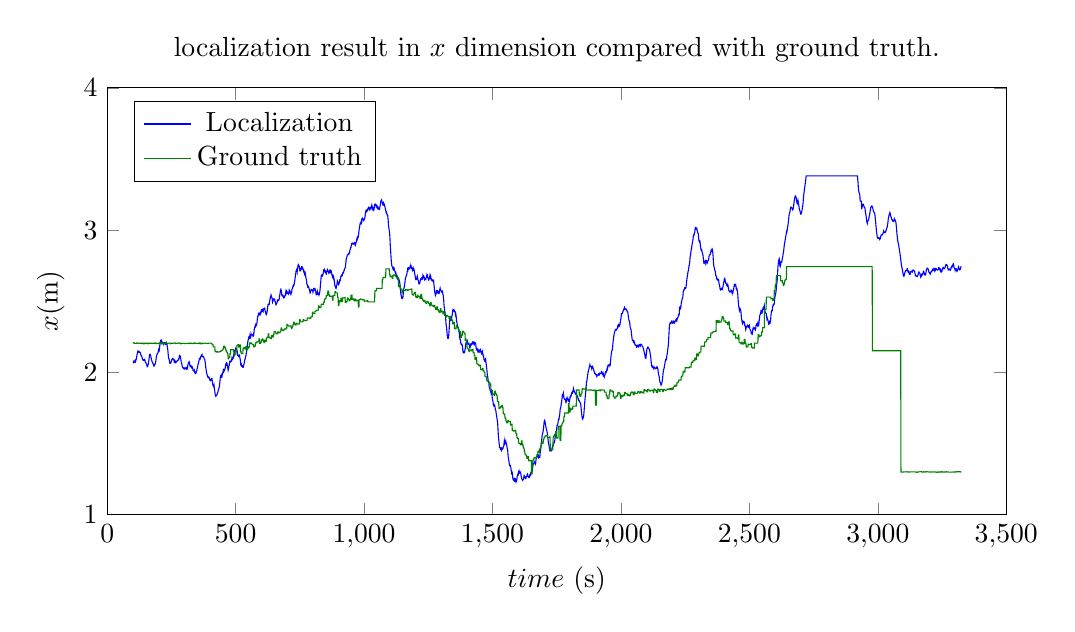
\begin{tikzpicture}

\begin{axis}[
title={localization result in $x$ dimension compared with ground truth.},
xlabel={$time$ (s)},
ylabel={$x$(m)},
xmin=0, xmax=3500,
ymin=1, ymax=4,
axis on top,
width=13cm,
height=7cm,
legend style={at={(0.03,0.97)}, anchor=north west},
legend entries={{Localization},{Ground truth}}
]
\addplot [blue]
coordinates {
(100,2.06431555747986)
(101,2.06523561477661)
(102,2.06774282455444)
(103,2.07627081871033)
(104,2.07920742034912)
(105,2.07356405258179)
(106,2.07174229621887)
(107,2.07393789291382)
(108,2.07418632507324)
(109,2.07914328575134)
(110,2.07410955429077)
(111,2.07941675186157)
(112,2.09041213989258)
(113,2.09065985679626)
(114,2.09987449645996)
(115,2.10877513885498)
(116,2.12272477149963)
(117,2.12799429893494)
(118,2.13773465156555)
(119,2.1462709903717)
(120,2.15050625801086)
(121,2.14887380599976)
(122,2.14683890342712)
(123,2.14279294013977)
(124,2.14069604873657)
(125,2.14002132415771)
(126,2.14315557479858)
(127,2.14165115356445)
(128,2.14062929153442)
(129,2.13757252693176)
(130,2.13195085525513)
(131,2.12361836433411)
(132,2.11759066581726)
(133,2.11657357215881)
(134,2.11384987831116)
(135,2.10838675498962)
(136,2.10419034957886)
(137,2.09351205825806)
(138,2.09191083908081)
(139,2.08886003494263)
(140,2.08354496955872)
(141,2.08382511138916)
(142,2.08541750907898)
(143,2.08756542205811)
(144,2.08526396751404)
(145,2.08402109146118)
(146,2.08863830566406)
(147,2.08464431762695)
(148,2.07350707054138)
(149,2.06981325149536)
(150,2.06928300857544)
(151,2.06556439399719)
(152,2.06202578544617)
(153,2.05938935279846)
(154,2.05125164985657)
(155,2.04765725135803)
(156,2.03903198242187)
(157,2.03915286064148)
(158,2.04411339759827)
(159,2.05064511299133)
(160,2.05747938156128)
(161,2.06888437271118)
(162,2.08215308189392)
(163,2.09356355667114)
(164,2.10829591751099)
(165,2.12507843971252)
(166,2.12700605392456)
(167,2.12734436988831)
(168,2.12297129631042)
(169,2.12013959884644)
(170,2.10954689979553)
(171,2.10191512107849)
(172,2.09263825416565)
(173,2.08665084838867)
(174,2.08008718490601)
(175,2.07282614707947)
(176,2.07061529159546)
(177,2.0692150592804)
(178,2.06169939041138)
(179,2.06047940254211)
(180,2.05395936965942)
(181,2.04804134368896)
(182,2.04338502883911)
(183,2.04389548301697)
(184,2.0492422580719)
(185,2.05612969398498)
(186,2.05890464782715)
(187,2.05873298645019)
(188,2.06510496139526)
(189,2.07675862312317)
(190,2.08982300758362)
(191,2.10260534286499)
(192,2.11218929290771)
(193,2.12115120887756)
(194,2.12514543533325)
(195,2.13068652153015)
(196,2.13279628753662)
(197,2.13441276550293)
(198,2.13978719711304)
(199,2.14889311790466)
(200,2.15676259994507)
(201,2.15169262886047)
(202,2.14926505088806)
(203,2.15796852111816)
(204,2.1731014251709)
(205,2.19177913665771)
(206,2.20320463180542)
(207,2.21744608879089)
(208,2.22413372993469)
(209,2.22431397438049)
(210,2.2200722694397)
(211,2.22513604164123)
(212,2.2212655544281)
(213,2.21728134155273)
(214,2.21094369888306)
(215,2.20310807228088)
(216,2.20155715942383)
(217,2.2052571773529)
(218,2.20665574073791)
(219,2.20777916908264)
(220,2.19995617866516)
(221,2.2065441608429)
(222,2.20481824874878)
(223,2.20643758773804)
(224,2.20392370223999)
(225,2.20612382888794)
(226,2.20338749885559)
(227,2.19577813148498)
(228,2.19746041297913)
(229,2.20323371887207)
(230,2.20789957046509)
(231,2.19984340667725)
(232,2.20104813575745)
(233,2.19515538215637)
(234,2.18059039115906)
(235,2.1694130897522)
(236,2.15819478034973)
(237,2.13785600662231)
(238,2.11641502380371)
(239,2.10175347328186)
(240,2.09401774406433)
(241,2.09375190734863)
(242,2.08248686790466)
(243,2.07140207290649)
(244,2.06239914894104)
(245,2.06329441070557)
(246,2.06330847740173)
(247,2.06539130210876)
(248,2.06802678108215)
(249,2.07444024085998)
(250,2.08118557929993)
(251,2.08661723136902)
(252,2.09117841720581)
(253,2.091721534729)
(254,2.09571719169617)
(255,2.09215140342712)
(256,2.09502959251404)
(257,2.09464168548584)
(258,2.09350967407227)
(259,2.09093189239502)
(260,2.08191919326782)
(261,2.07330274581909)
(262,2.07693862915039)
(263,2.0837938785553)
(264,2.08190321922302)
(265,2.07345795631409)
(266,2.06762719154358)
(267,2.06804537773132)
(268,2.07031345367432)
(269,2.07256960868835)
(270,2.07734417915344)
(271,2.07750153541565)
(272,2.0779869556427)
(273,2.08169841766357)
(274,2.08182406425476)
(275,2.08406233787537)
(276,2.08539628982544)
(277,2.08585953712463)
(278,2.09355616569519)
(279,2.09213471412659)
(280,2.1009578704834)
(281,2.11610770225525)
(282,2.11916661262512)
(283,2.1178867816925)
(284,2.11582136154175)
(285,2.10597848892212)
(286,2.09940838813782)
(287,2.08848309516907)
(288,2.07348132133484)
(289,2.06670308113098)
(290,2.06205606460571)
(291,2.05346918106079)
(292,2.04565787315369)
(293,2.03592967987061)
(294,2.03486847877502)
(295,2.03237533569336)
(296,2.02878546714783)
(297,2.03043055534363)
(298,2.02727246284485)
(299,2.02373695373535)
(300,2.02338337898254)
(301,2.02862572669983)
(302,2.0259108543396)
(303,2.02406668663025)
(304,2.02469444274902)
(305,2.02607798576355)
(306,2.03179121017456)
(307,2.03405928611755)
(308,2.02985858917236)
(309,2.02171015739441)
(310,2.02135896682739)
(311,2.02182221412659)
(312,2.02587652206421)
(313,2.03975605964661)
(314,2.0497031211853)
(315,2.05657410621643)
(316,2.06410956382751)
(317,2.06869292259216)
(318,2.07182765007019)
(319,2.07460594177246)
(320,2.06737041473389)
(321,2.05989241600037)
(322,2.0460352897644)
(323,2.03982973098755)
(324,2.04029440879822)
(325,2.04395699501038)
(326,2.04568910598755)
(327,2.04082369804382)
(328,2.03612995147705)
(329,2.04214715957642)
(330,2.04188084602356)
(331,2.03698492050171)
(332,2.03081393241882)
(333,2.02662634849548)
(334,2.01389479637146)
(335,2.0123131275177)
(336,2.00921416282654)
(337,2.00998950004578)
(338,2.011146068573)
(339,2.01524376869202)
(340,2.00718903541565)
(341,1.99942636489868)
(342,2.00112056732178)
(343,1.9938839673996)
(344,1.99469912052155)
(345,1.99212324619293)
(346,1.99719655513763)
(347,2.00181460380554)
(348,2.00951957702637)
(349,2.01377367973328)
(350,2.02448582649231)
(351,2.02908253669739)
(352,2.03631925582886)
(353,2.04880309104919)
(354,2.06057691574097)
(355,2.06215405464172)
(356,2.0688784122467)
(357,2.07815432548523)
(358,2.09019088745117)
(359,2.09664082527161)
(360,2.09814643859863)
(361,2.09937691688538)
(362,2.09563112258911)
(363,2.10449981689453)
(364,2.1099898815155)
(365,2.10923981666565)
(366,2.11326003074646)
(367,2.11880707740784)
(368,2.12362504005432)
(369,2.12595725059509)
(370,2.11131882667541)
(371,2.10882592201233)
(372,2.10855197906494)
(373,2.10865139961243)
(374,2.11145448684692)
(375,2.11017441749573)
(376,2.10710644721985)
(377,2.09918236732483)
(378,2.09368443489075)
(379,2.09310555458069)
(380,2.08543395996094)
(381,2.07770299911499)
(382,2.06320548057556)
(383,2.04762148857117)
(384,2.03010249137878)
(385,2.02094841003418)
(386,2.00583982467651)
(387,1.99361264705658)
(388,1.98883020877838)
(389,1.98430097103119)
(390,1.97761821746826)
(391,1.97072780132294)
(392,1.96504414081573)
(393,1.96258795261383)
(394,1.96282851696014)
(395,1.96139681339264)
(396,1.96575534343719)
(397,1.96223378181458)
(398,1.95528924465179)
(399,1.9471869468689)
(400,1.94743824005127)
(401,1.94356083869934)
(402,1.94140291213989)
(403,1.94427478313446)
(404,1.94945347309113)
(405,1.95277905464172)
(406,1.95248162746429)
(407,1.95648765563965)
(408,1.95528161525726)
(409,1.94017958641052)
(410,1.92716860771179)
(411,1.91545939445496)
(412,1.90739607810974)
(413,1.90351188182831)
(414,1.90295553207397)
(415,1.89801025390625)
(416,1.90698909759521)
(417,1.89169669151306)
(418,1.87766265869141)
(419,1.86506164073944)
(420,1.85075032711029)
(421,1.83783435821533)
(422,1.83462357521057)
(423,1.83916819095612)
(424,1.8376350402832)
(425,1.83562934398651)
(426,1.83889770507812)
(427,1.83954215049744)
(428,1.84708058834076)
(429,1.85091364383698)
(430,1.85771751403809)
(431,1.86037886142731)
(432,1.87001013755798)
(433,1.87914729118347)
(434,1.88308525085449)
(435,1.88668811321259)
(436,1.89416360855103)
(437,1.90720283985138)
(438,1.92034924030304)
(439,1.93834817409515)
(440,1.95908999443054)
(441,1.96837711334229)
(442,1.96402835845947)
(443,1.9653947353363)
(444,1.97453856468201)
(445,1.96690058708191)
(446,1.96491312980652)
(447,1.97193217277527)
(448,1.98450231552124)
(449,1.99394488334656)
(450,1.99262511730194)
(451,1.99766290187836)
(452,2.01469874382019)
(453,2.02133965492248)
(454,2.0209596157074)
(455,2.00886106491089)
(456,2.01346182823181)
(457,2.01506042480469)
(458,2.02032041549683)
(459,2.02570343017578)
(460,2.03787088394165)
(461,2.05448007583618)
(462,2.05838394165039)
(463,2.05548167228699)
(464,2.06589317321777)
(465,2.06720900535583)
(466,2.06626033782959)
(467,2.0563805103302)
(468,2.03992342948914)
(469,2.03958177566528)
(470,2.0274224281311)
(471,2.01494264602661)
(472,2.02198696136475)
(473,2.03366231918335)
(474,2.04725432395935)
(475,2.04977369308472)
(476,2.06262803077698)
(477,2.07284045219421)
(478,2.06942129135132)
(479,2.07280564308166)
(480,2.07603764533997)
(481,2.07614326477051)
(482,2.08008360862732)
(483,2.08414220809936)
(484,2.08173727989197)
(485,2.09328532218933)
(486,2.10305619239807)
(487,2.0978684425354)
(488,2.09327936172485)
(489,2.0974702835083)
(490,2.09803605079651)
(491,2.10371112823486)
(492,2.11178970336914)
(493,2.12327122688293)
(494,2.13384127616882)
(495,2.12096881866455)
(496,2.12632060050964)
(497,2.1383683681488)
(498,2.14960122108459)
(499,2.16015958786011)
(500,2.1679699420929)
(501,2.17154383659363)
(502,2.166175365448)
(503,2.1616005897522)
(504,2.15513944625854)
(505,2.15602493286133)
(506,2.14766955375671)
(507,2.13719415664673)
(508,2.11864113807678)
(509,2.11756443977356)
(510,2.11970162391663)
(511,2.11980032920837)
(512,2.11038088798523)
(513,2.11082601547241)
(514,2.11666917800903)
(515,2.11890721321106)
(516,2.10819506645203)
(517,2.0980052947998)
(518,2.08893513679504)
(519,2.07245969772339)
(520,2.05531549453735)
(521,2.04786396026611)
(522,2.04578351974487)
(523,2.05171728134155)
(524,2.04427790641785)
(525,2.04478406906128)
(526,2.04574608802795)
(527,2.03912091255188)
(528,2.03420305252075)
(529,2.03379321098328)
(530,2.03796553611755)
(531,2.04908990859985)
(532,2.05351328849792)
(533,2.06006574630737)
(534,2.07244229316711)
(535,2.08632278442383)
(536,2.08921265602112)
(537,2.09279084205627)
(538,2.10235643386841)
(539,2.11243391036987)
(540,2.11466312408447)
(541,2.1279444694519)
(542,2.13923931121826)
(543,2.15825605392456)
(544,2.16820335388184)
(545,2.17831993103027)
(546,2.19342303276062)
(547,2.21150374412537)
(548,2.21942257881165)
(549,2.22775387763977)
(550,2.23782205581665)
(551,2.2466037273407)
(552,2.25003147125244)
(553,2.24795198440552)
(554,2.24400281906128)
(555,2.2544891834259)
(556,2.24438762664795)
(557,2.24107217788696)
(558,2.24364447593689)
(559,2.25081634521484)
(560,2.27042388916016)
(561,2.26431798934936)
(562,2.26351070404053)
(563,2.26216173171997)
(564,2.26238965988159)
(565,2.26258015632629)
(566,2.26203560829163)
(567,2.25794386863708)
(568,2.26308703422546)
(569,2.25485944747925)
(570,2.25711607933044)
(571,2.27146005630493)
(572,2.29202580451965)
(573,2.30878281593323)
(574,2.31227135658264)
(575,2.31852293014526)
(576,2.32846450805664)
(577,2.32769560813904)
(578,2.33363461494446)
(579,2.32554888725281)
(580,2.32943105697632)
(581,2.33054947853088)
(582,2.33791589736938)
(583,2.3468325138092)
(584,2.36464262008667)
(585,2.38341856002808)
(586,2.3919141292572)
(587,2.39345622062683)
(588,2.40002202987671)
(589,2.41243696212769)
(590,2.4128851890564)
(591,2.41814732551575)
(592,2.41820216178894)
(593,2.41794610023498)
(594,2.40330410003662)
(595,2.40199756622314)
(596,2.41099524497986)
(597,2.41813540458679)
(598,2.42434191703796)
(599,2.41959047317505)
(600,2.4259192943573)
(601,2.43968152999878)
(602,2.44091701507568)
(603,2.43489575386047)
(604,2.43979334831238)
(605,2.43485617637634)
(606,2.4289345741272)
(607,2.42643666267395)
(608,2.43715119361877)
(609,2.44544267654419)
(610,2.44807529449463)
(611,2.44638586044311)
(612,2.44940757751465)
(613,2.45100498199463)
(614,2.44064784049988)
(615,2.4304141998291)
(616,2.42360472679138)
(617,2.41925144195557)
(618,2.41152262687683)
(619,2.40539693832397)
(620,2.40786361694336)
(621,2.4105064868927)
(622,2.4247510433197)
(623,2.43176794052124)
(624,2.44741749763489)
(625,2.46200180053711)
(626,2.47506308555603)
(627,2.47786426544189)
(628,2.47489714622498)
(629,2.47568011283874)
(630,2.47608470916748)
(631,2.47858047485352)
(632,2.49081563949585)
(633,2.5030300617218)
(634,2.51375246047974)
(635,2.52230167388916)
(636,2.53153848648071)
(637,2.53534698486328)
(638,2.54347395896912)
(639,2.53777837753296)
(640,2.53012776374817)
(641,2.52376556396484)
(642,2.52172827720642)
(643,2.51039123535156)
(644,2.49342656135559)
(645,2.49816703796387)
(646,2.50852346420288)
(647,2.51284003257751)
(648,2.51013255119324)
(649,2.5103108882904)
(650,2.51585626602173)
(651,2.51563572883606)
(652,2.50998759269714)
(653,2.4990074634552)
(654,2.49816274642944)
(655,2.4884467124939)
(656,2.4786901473999)
(657,2.47475862503052)
(658,2.47868704795837)
(659,2.4823625087738)
(660,2.48801827430725)
(661,2.48856520652771)
(662,2.49728536605835)
(663,2.50833034515381)
(664,2.50692415237427)
(665,2.50615382194519)
(666,2.50494742393494)
(667,2.50967526435852)
(668,2.51162266731262)
(669,2.51046323776245)
(670,2.5194718837738)
(671,2.53497195243835)
(672,2.54505586624145)
(673,2.55396056175232)
(674,2.56696462631226)
(675,2.57891201972961)
(676,2.58324432373047)
(677,2.57681536674499)
(678,2.57286787033081)
(679,2.56006693840027)
(680,2.53912448883057)
(681,2.5369246006012)
(682,2.53630423545837)
(683,2.53801155090332)
(684,2.54037594795227)
(685,2.53672003746033)
(686,2.52902936935425)
(687,2.53149747848511)
(688,2.52565836906433)
(689,2.52925157546997)
(690,2.52871894836426)
(691,2.53738689422607)
(692,2.53949594497681)
(693,2.53895020484924)
(694,2.55115556716919)
(695,2.5637321472168)
(696,2.57214999198914)
(697,2.5661997795105)
(698,2.56079936027527)
(699,2.57114553451538)
(700,2.56834650039673)
(701,2.5637629032135)
(702,2.55716824531555)
(703,2.5573399066925)
(704,2.55299115180969)
(705,2.54853558540344)
(706,2.55157160758972)
(707,2.55814290046692)
(708,2.56962466239929)
(709,2.56077861785889)
(710,2.56431341171265)
(711,2.57260060310364)
(712,2.56919431686401)
(713,2.56404399871826)
(714,2.55088353157043)
(715,2.54729461669922)
(716,2.55555367469788)
(717,2.55798697471619)
(718,2.56042981147766)
(719,2.57712435722351)
(720,2.58743262290955)
(721,2.59001779556274)
(722,2.59504127502441)
(723,2.60518741607666)
(724,2.60913610458374)
(725,2.60396242141724)
(726,2.60556674003601)
(727,2.61438298225403)
(728,2.61934733390808)
(729,2.628910779953)
(730,2.64096617698669)
(731,2.65485048294067)
(732,2.67005753517151)
(733,2.68480348587036)
(734,2.69188046455383)
(735,2.7097864151001)
(736,2.71530961990356)
(737,2.71762704849243)
(738,2.72458028793335)
(739,2.72800850868225)
(740,2.7127034664154)
(741,2.73111081123352)
(742,2.74020504951477)
(743,2.75150060653686)
(744,2.75768494606018)
(745,2.75456094741821)
(746,2.75055074691772)
(747,2.74721050262451)
(748,2.73986649513245)
(749,2.72502326965332)
(750,2.71530699729919)
(751,2.71692872047424)
(752,2.71527075767517)
(753,2.71407961845398)
(754,2.72219443321228)
(755,2.73617553710937)
(756,2.74167799949646)
(757,2.74034118652344)
(758,2.73381972312927)
(759,2.74010825157165)
(760,2.73699641227722)
(761,2.73315000534058)
(762,2.72616052627563)
(763,2.72542381286621)
(764,2.71614027023315)
(765,2.70576095581055)
(766,2.70256280899048)
(767,2.70766258239746)
(768,2.69893097877502)
(769,2.68753027915955)
(770,2.69031167030334)
(771,2.69664525985718)
(772,2.68661332130432)
(773,2.67386722564697)
(774,2.66307330131531)
(775,2.6565477848053)
(776,2.64184284210205)
(777,2.62330555915832)
(778,2.6175742149353)
(779,2.61558747291565)
(780,2.60939455032349)
(781,2.59793591499329)
(782,2.59909296035767)
(783,2.60330510139465)
(784,2.60064601898193)
(785,2.59434938430786)
(786,2.58679676055908)
(787,2.58334493637085)
(788,2.58125329017639)
(789,2.56493377685547)
(790,2.55771112442017)
(791,2.56107044219971)
(792,2.56857943534851)
(793,2.57627058029175)
(794,2.57544755935669)
(795,2.57783079147339)
(796,2.58154034614563)
(797,2.57921552658081)
(798,2.57782459259033)
(799,2.57733035087585)
(800,2.57299971580505)
(801,2.56310176849365)
(802,2.57089757919311)
(803,2.57904815673828)
(804,2.58930778503418)
(805,2.5906994342804)
(806,2.58663010597229)
(807,2.5826473236084)
(808,2.58763217926025)
(809,2.58818483352661)
(810,2.57997488975525)
(811,2.56861805915832)
(812,2.56482839584351)
(813,2.55307555198669)
(814,2.54509520530701)
(815,2.5454843044281)
(816,2.55165123939514)
(817,2.55837440490723)
(818,2.56984925270081)
(819,2.56163549423218)
(820,2.55192923545837)
(821,2.5541033744812)
(822,2.55037617683411)
(823,2.55119490623474)
(824,2.5453360080719)
(825,2.55388736724853)
(826,2.55094313621521)
(827,2.55954575538635)
(828,2.56998658180237)
(829,2.5885705947876)
(830,2.6088342666626)
(831,2.63152718544006)
(832,2.65080261230469)
(833,2.67322540283203)
(834,2.68365144729614)
(835,2.68440222740173)
(836,2.6808774471283)
(837,2.68631386756897)
(838,2.68590831756592)
(839,2.68199682235718)
(840,2.68951749801636)
(841,2.69716453552246)
(842,2.71128869056702)
(843,2.72000241279602)
(844,2.718581199646)
(845,2.72002696990967)
(846,2.72316670417786)
(847,2.71359300613403)
(848,2.70395421981811)
(849,2.70300340652466)
(850,2.70656228065491)
(851,2.6993043422699)
(852,2.69356036186218)
(853,2.69201564788818)
(854,2.70896911621094)
(855,2.71138215065002)
(856,2.70993447303772)
(857,2.70954394340515)
(858,2.720862865448)
(859,2.71715331077576)
(860,2.71212339401245)
(861,2.70676326751709)
(862,2.70104193687439)
(863,2.69649529457092)
(864,2.70024609565735)
(865,2.70109486579895)
(866,2.7141056060791)
(867,2.71885895729065)
(868,2.72000670433044)
(869,2.70888423919678)
(870,2.71452856063843)
(871,2.71464085578918)
(872,2.71243500709534)
(873,2.7044095993042)
(874,2.6925163269043)
(875,2.68609285354614)
(876,2.6786630153656)
(877,2.66807293891907)
(878,2.66482973098755)
(879,2.66753268241882)
(880,2.67875838279724)
(881,2.67560029029846)
(882,2.65520572662353)
(883,2.65716171264648)
(884,2.64661431312561)
(885,2.62813448905945)
(886,2.61456418037415)
(887,2.60610198974609)
(888,2.60153889656067)
(889,2.59969902038574)
(890,2.59094452857971)
(891,2.58960032463074)
(892,2.59886813163757)
(893,2.61094760894775)
(894,2.61261320114136)
(895,2.62625551223755)
(896,2.64291191101074)
(897,2.63836359977722)
(898,2.63196110725403)
(899,2.62882542610168)
(900,2.62317371368408)
(901,2.61702370643616)
(902,2.62009572982788)
(903,2.62622594833374)
(904,2.63490486145019)
(905,2.64556813240051)
(906,2.64296913146973)
(907,2.64424753189087)
(908,2.66001868247986)
(909,2.67012524604797)
(910,2.6710352897644)
(911,2.68109846115112)
(912,2.68317937850952)
(913,2.67806458473206)
(914,2.67744469642639)
(915,2.6797821521759)
(916,2.68986988067627)
(917,2.69905614852905)
(918,2.70188045501709)
(919,2.70154309272766)
(920,2.70016551017761)
(921,2.70873475074768)
(922,2.71782231330872)
(923,2.71787691116333)
(924,2.72518110275269)
(925,2.73088383674622)
(926,2.73263692855835)
(927,2.73958897590637)
(928,2.75155520439148)
(929,2.7684121131897)
(930,2.7871618270874)
(931,2.80047225952148)
(932,2.80418038368225)
(933,2.80845785140991)
(934,2.81877541542053)
(935,2.82591462135315)
(936,2.82619881629944)
(937,2.82672381401062)
(938,2.8292384147644)
(939,2.83252596855164)
(940,2.83522510528564)
(941,2.83146977424622)
(942,2.83518052101135)
(943,2.84066700935364)
(944,2.84663724899292)
(945,2.85971403121948)
(946,2.86222743988037)
(947,2.87033605575561)
(948,2.87746787071228)
(949,2.87815809249878)
(950,2.88781595230102)
(951,2.89495515823364)
(952,2.90597176551819)
(953,2.90556073188782)
(954,2.90784764289856)
(955,2.90884566307068)
(956,2.90741229057312)
(957,2.90386700630188)
(958,2.90056872367859)
(959,2.9009325504303)
(960,2.90696239471436)
(961,2.90894436836243)
(962,2.91021776199341)
(963,2.91175651550293)
(964,2.90508580207825)
(965,2.90049886703491)
(966,2.89480757713318)
(967,2.90050148963928)
(968,2.90761208534241)
(969,2.91400337219238)
(970,2.9172203540802)
(971,2.92930865287781)
(972,2.93892002105713)
(973,2.94531774520874)
(974,2.93740725517273)
(975,2.94363808631897)
(976,2.94646334648132)
(977,2.94694638252258)
(978,2.95837759971619)
(979,2.97602295875549)
(980,2.99042224884033)
(981,3.00516176223755)
(982,3.01341247558594)
(983,3.02536797523498)
(984,3.03812837600708)
(985,3.04807782173157)
(986,3.04753255844116)
(987,3.05228495597839)
(988,3.05251288414001)
(989,3.06041932106018)
(990,3.0497944355011)
(991,3.05363845825195)
(992,3.07368278503418)
(993,3.08328676223755)
(994,3.07959032058716)
(995,3.0769419670105)
(996,3.07827186584473)
(997,3.07459044456482)
(998,3.07143354415894)
(999,3.06688833236694)
(1000,3.07197761535644)
(1001,3.07740235328674)
(1002,3.07947468757629)
(1003,3.08687663078308)
(1004,3.09875535964966)
(1005,3.11292266845703)
(1006,3.12648630142212)
(1007,3.13579511642456)
(1008,3.13964080810547)
(1009,3.13739442825317)
(1010,3.13311672210693)
(1011,3.13782048225403)
(1012,3.14186978340149)
(1013,3.1442711353302)
(1014,3.1411771774292)
(1015,3.15055155754089)
(1016,3.15525078773498)
(1017,3.15630412101746)
(1018,3.15924644470215)
(1019,3.15134048461914)
(1020,3.15133285522461)
(1021,3.14215517044067)
(1022,3.14104294776916)
(1023,3.15225768089294)
(1024,3.15916156768799)
(1025,3.16032314300537)
(1026,3.15834593772888)
(1027,3.15369987487793)
(1028,3.16416811943054)
(1029,3.16960263252258)
(1030,3.17678260803223)
(1031,3.17026925086975)
(1032,3.16010689735413)
(1033,3.15481901168823)
(1034,3.14424562454224)
(1035,3.1395742893219)
(1036,3.1462926864624)
(1037,3.15548396110535)
(1038,3.15447473526001)
(1039,3.1498372554779)
(1040,3.16719317436218)
(1041,3.17641305923462)
(1042,3.18133163452148)
(1043,3.18352627754211)
(1044,3.18347644805908)
(1045,3.18201780319214)
(1046,3.17225384712219)
(1047,3.16648411750793)
(1048,3.17397165298462)
(1049,3.17112421989441)
(1050,3.17243576049805)
(1051,3.16337656974792)
(1052,3.15766549110413)
(1053,3.16366314888)
(1054,3.16406941413879)
(1055,3.14873909950256)
(1056,3.14898777008057)
(1057,3.1519558429718)
(1058,3.14934754371643)
(1059,3.14377355575561)
(1060,3.143714427948)
(1061,3.15740585327148)
(1062,3.16630434989929)
(1063,3.17629170417786)
(1064,3.1837899684906)
(1065,3.19814014434814)
(1066,3.20773577690124)
(1067,3.20848083496094)
(1068,3.21210289001465)
(1069,3.20071482658386)
(1070,3.19904613494873)
(1071,3.19481492042541)
(1072,3.18437385559082)
(1073,3.17947697639465)
(1074,3.18564462661743)
(1075,3.19094800949097)
(1076,3.18274736404419)
(1077,3.17857646942139)
(1078,3.18442702293396)
(1079,3.18348169326782)
(1080,3.1708459854126)
(1081,3.16413617134094)
(1082,3.15722155570984)
(1083,3.14765501022339)
(1084,3.13812875747681)
(1085,3.13309860229492)
(1086,3.12356042861938)
(1087,3.12530565261841)
(1088,3.11642861366272)
(1089,3.11494922637939)
(1090,3.10763621330261)
(1091,3.10805940628052)
(1092,3.10228276252747)
(1093,3.08319807052612)
(1094,3.062424659729)
(1095,3.03555393218994)
(1096,3.02108788490295)
(1097,3.0100953578949)
(1098,2.9956419467926)
(1099,2.98498725891113)
(1100,2.96475863456726)
(1101,2.93183732032776)
(1102,2.89413690567017)
(1103,2.86360859870911)
(1104,2.8392539024353)
(1105,2.80741310119629)
(1106,2.78299069404602)
(1107,2.76088571548462)
(1108,2.7520158290863)
(1109,2.74391436576843)
(1110,2.7403552532196)
(1111,2.73984932899475)
(1112,2.73064017295837)
(1113,2.72418880462646)
(1114,2.72173976898193)
(1115,2.72919392585754)
(1116,2.73550629615784)
(1117,2.73291325569153)
(1118,2.71697211265564)
(1119,2.71421051025391)
(1120,2.71159815788269)
(1121,2.70601272583008)
(1122,2.69779968261719)
(1123,2.69379377365112)
(1124,2.69831824302673)
(1125,2.69121336936951)
(1126,2.67501044273376)
(1127,2.66803383827209)
(1128,2.67009115219116)
(1129,2.67378282546997)
(1130,2.66031408309936)
(1131,2.65371990203857)
(1132,2.65174293518066)
(1133,2.64853882789612)
(1134,2.64775800704956)
(1135,2.64563679695129)
(1136,2.65187048912048)
(1137,2.64634799957275)
(1138,2.63983178138733)
(1139,2.62762379646301)
(1140,2.61303901672363)
(1141,2.59178161621094)
(1142,2.57549166679382)
(1143,2.55439901351929)
(1144,2.54513835906982)
(1145,2.53639626502991)
(1146,2.52867913246155)
(1147,2.51967430114746)
(1148,2.51860284805298)
(1149,2.51783609390259)
(1150,2.51910209655762)
(1151,2.52730345726013)
(1152,2.53966164588928)
(1153,2.56121897697449)
(1154,2.58104419708252)
(1155,2.59160685539246)
(1156,2.59592294692993)
(1157,2.6049702167511)
(1158,2.6178023815155)
(1159,2.62936902046204)
(1160,2.6462197303772)
(1161,2.65996170043945)
(1162,2.66659426689148)
(1163,2.67160367965698)
(1164,2.6775586605072)
(1165,2.67979550361633)
(1166,2.6858983039856)
(1167,2.69774198532104)
(1168,2.70706868171692)
(1169,2.72056460380554)
(1170,2.73257327079773)
(1171,2.73395848274231)
(1172,2.72538661956787)
(1173,2.73296976089477)
(1174,2.73463773727417)
(1175,2.7342414855957)
(1176,2.72902846336365)
(1177,2.73158836364746)
(1178,2.73497581481934)
(1179,2.74187850952148)
(1180,2.73811793327331)
(1181,2.74586391448975)
(1182,2.75425624847412)
(1183,2.7490074634552)
(1184,2.74060344696045)
(1185,2.73334455490112)
(1186,2.73655128479004)
(1187,2.73240423202515)
(1188,2.72194695472717)
(1189,2.7295126914978)
(1190,2.7272424697876)
(1191,2.73211908340454)
(1192,2.72012281417847)
(1193,2.72209143638611)
(1194,2.72491669654846)
(1195,2.71739840507507)
(1196,2.70745372772217)
(1197,2.69362378120422)
(1198,2.68678569793701)
(1199,2.67424321174622)
(1200,2.65963959693909)
(1201,2.65457940101623)
(1202,2.65147638320923)
(1203,2.65226912498474)
(1204,2.65285968780518)
(1205,2.65918588638306)
(1206,2.67008662223816)
(1207,2.67692279815674)
(1208,2.67104935646057)
(1209,2.65789031982422)
(1210,2.64756369590759)
(1211,2.64422702789307)
(1212,2.63981080055237)
(1213,2.62712359428406)
(1214,2.62145447731018)
(1215,2.62130689620972)
(1216,2.62435293197632)
(1217,2.62899136543274)
(1218,2.63659453392029)
(1219,2.64956498146057)
(1220,2.6547486782074)
(1221,2.65845155715942)
(1222,2.65796446800232)
(1223,2.65948104858398)
(1224,2.66246199607849)
(1225,2.65198302268982)
(1226,2.65232276916504)
(1227,2.6567075252533)
(1228,2.66189479827881)
(1229,2.67814493179321)
(1230,2.67160153388977)
(1231,2.67471790313721)
(1232,2.67676711082458)
(1233,2.66755056381226)
(1234,2.66135692596436)
(1235,2.65378069877624)
(1236,2.65902304649353)
(1237,2.6539158821106)
(1238,2.65237665176392)
(1239,2.65167093276977)
(1240,2.65118622779846)
(1241,2.66256165504456)
(1242,2.66649460792541)
(1243,2.67214035987854)
(1244,2.68129086494446)
(1245,2.68935775756836)
(1246,2.68739438056946)
(1247,2.67130136489868)
(1248,2.66481137275696)
(1249,2.66222715377808)
(1250,2.65846228599548)
(1251,2.64785504341125)
(1252,2.6482048034668)
(1253,2.65573573112488)
(1254,2.66676020622253)
(1255,2.66478800773621)
(1256,2.67817783355713)
(1257,2.687260389328)
(1258,2.68179059028625)
(1259,2.68044137954712)
(1260,2.66017293930054)
(1261,2.65480446815491)
(1262,2.65662288665771)
(1263,2.65329313278198)
(1264,2.64454174041748)
(1265,2.64215540885925)
(1266,2.64580774307251)
(1267,2.64996647834778)
(1268,2.64984726905823)
(1269,2.6500871181488)
(1270,2.64928913116455)
(1271,2.63827466964722)
(1272,2.61746048927307)
(1273,2.60193252563477)
(1274,2.58434581756592)
(1275,2.5688157081604)
(1276,2.5562846660614)
(1277,2.54643321037292)
(1278,2.54072856903076)
(1279,2.54667186737061)
(1280,2.55050325393677)
(1281,2.55770564079285)
(1282,2.57506608963013)
(1283,2.57519745826721)
(1284,2.57170009613037)
(1285,2.56630158424377)
(1286,2.56238389015198)
(1287,2.5673201084137)
(1288,2.55999493598938)
(1289,2.55469083786011)
(1290,2.55640864372253)
(1291,2.56175708770752)
(1292,2.56652808189392)
(1293,2.56292963027954)
(1294,2.57604336738586)
(1295,2.58437371253967)
(1296,2.59105825424194)
(1297,2.58213567733765)
(1298,2.57851243019104)
(1299,2.57773661613464)
(1300,2.57309293746948)
(1301,2.56568598747253)
(1302,2.56339883804321)
(1303,2.56376719474792)
(1304,2.56895065307617)
(1305,2.57075357437134)
(1306,2.55942797660828)
(1307,2.54881048202515)
(1308,2.54159712791443)
(1309,2.52676630020142)
(1310,2.50828552246094)
(1311,2.47812509536743)
(1312,2.46089148521423)
(1313,2.44557666778564)
(1314,2.43048167228699)
(1315,2.42100620269775)
(1316,2.40624117851257)
(1317,2.39256429672241)
(1318,2.36778521537781)
(1319,2.34035301208496)
(1320,2.32758545875549)
(1321,2.31738018989563)
(1322,2.29905581474304)
(1323,2.27673506736755)
(1324,2.25744295120239)
(1325,2.24595284461975)
(1326,2.23911690711975)
(1327,2.23772025108337)
(1328,2.23899292945862)
(1329,2.24739027023315)
(1330,2.27095651626587)
(1331,2.29235315322876)
(1332,2.32717943191528)
(1333,2.35608959197998)
(1334,2.37439656257629)
(1335,2.37819886207581)
(1336,2.37026524543762)
(1337,2.36553692817688)
(1338,2.36656475067139)
(1339,2.3664493560791)
(1340,2.37354207038879)
(1341,2.38698554039001)
(1342,2.39809346199036)
(1343,2.40078997611999)
(1344,2.41345477104187)
(1345,2.43381977081299)
(1346,2.43942761421204)
(1347,2.43556451797485)
(1348,2.43331527709961)
(1349,2.44029474258423)
(1350,2.43986654281616)
(1351,2.43566918373108)
(1352,2.42842960357666)
(1353,2.42954468727112)
(1354,2.42675709724426)
(1355,2.41759157180786)
(1356,2.40575790405273)
(1357,2.41141819953918)
(1358,2.40084791183472)
(1359,2.38157677650452)
(1360,2.36146950721741)
(1361,2.35314035415649)
(1362,2.34705662727356)
(1363,2.33034038543701)
(1364,2.31823372840881)
(1365,2.31621646881103)
(1366,2.3110933303833)
(1367,2.30279493331909)
(1368,2.30042266845703)
(1369,2.29821395874023)
(1370,2.29043865203857)
(1371,2.26470184326172)
(1372,2.24271249771118)
(1373,2.2377188205719)
(1374,2.22979116439819)
(1375,2.2288932800293)
(1376,2.21060681343079)
(1377,2.20111989974976)
(1378,2.19687128067017)
(1379,2.1993556022644)
(1380,2.19903898239136)
(1381,2.19534254074097)
(1382,2.19268870353699)
(1383,2.18207406997681)
(1384,2.16386127471924)
(1385,2.14519739151001)
(1386,2.14723801612854)
(1387,2.14100050926208)
(1388,2.14151763916016)
(1389,2.13643956184387)
(1390,2.13833379745483)
(1391,2.13870596885681)
(1392,2.14923572540283)
(1393,2.15971827507019)
(1394,2.16884040832519)
(1395,2.18644618988037)
(1396,2.20119595527649)
(1397,2.19824862480164)
(1398,2.19856357574463)
(1399,2.20476126670837)
(1400,2.21306252479553)
(1401,2.22684240341186)
(1402,2.22357082366943)
(1403,2.21355605125427)
(1404,2.20188689231873)
(1405,2.19727444648743)
(1406,2.19747996330261)
(1407,2.20213341712952)
(1408,2.20346355438232)
(1409,2.1969141960144)
(1410,2.1884114742279)
(1411,2.1722149848938)
(1412,2.1709725856781)
(1413,2.17863368988037)
(1414,2.19215703010559)
(1415,2.19619727134705)
(1416,2.19176912307739)
(1417,2.19119620323181)
(1418,2.19462847709656)
(1419,2.20162916183472)
(1420,2.20363831520081)
(1421,2.20921683311462)
(1422,2.21141457557678)
(1423,2.20146560668945)
(1424,2.19902086257935)
(1425,2.20929145812988)
(1426,2.2139937877655)
(1427,2.21429872512817)
(1428,2.2104914188385)
(1429,2.20573782920837)
(1430,2.19916272163391)
(1431,2.20609402656555)
(1432,2.20344591140747)
(1433,2.203773021698)
(1434,2.20497965812683)
(1435,2.19726157188415)
(1436,2.17625117301941)
(1437,2.16414070129394)
(1438,2.16916227340698)
(1439,2.16809511184692)
(1440,2.16718482971191)
(1441,2.16208529472351)
(1442,2.15399503707886)
(1443,2.14545559883118)
(1444,2.14102530479431)
(1445,2.14294528961182)
(1446,2.1496889591217)
(1447,2.15703082084656)
(1448,2.15334510803223)
(1449,2.15016508102417)
(1450,2.14366912841797)
(1451,2.14541244506836)
(1452,2.1531229019165)
(1453,2.15857577323914)
(1454,2.15231895446777)
(1455,2.14595007896423)
(1456,2.13644242286682)
(1457,2.13239431381226)
(1458,2.1400716304779)
(1459,2.13952779769897)
(1460,2.14693784713745)
(1461,2.14944839477539)
(1462,2.1305205821991)
(1463,2.11835193634033)
(1464,2.11517739295959)
(1465,2.11692357063293)
(1466,2.10203266143799)
(1467,2.0892276763916)
(1468,2.08593010902405)
(1469,2.07953763008118)
(1470,2.07837152481079)
(1471,2.08569836616516)
(1472,2.09367752075195)
(1473,2.095778465271)
(1474,2.07842445373535)
(1475,2.06198143959045)
(1476,2.05028200149536)
(1477,2.03150248527527)
(1478,2.02188634872436)
(1479,1.99741983413696)
(1480,1.97852385044098)
(1481,1.97225916385651)
(1482,1.95869517326355)
(1483,1.94349944591522)
(1484,1.93843126296997)
(1485,1.93491899967194)
(1486,1.91965711116791)
(1487,1.89982855319977)
(1488,1.89137196540833)
(1489,1.89267301559448)
(1490,1.87929093837738)
(1491,1.87142598628998)
(1492,1.87000966072083)
(1493,1.8675103187561)
(1494,1.85740804672241)
(1495,1.86587178707123)
(1496,1.87103664875031)
(1497,1.86695635318756)
(1498,1.8447493314743)
(1499,1.82067584991455)
(1500,1.80648994445801)
(1501,1.80100452899933)
(1502,1.79438173770905)
(1503,1.77750277519226)
(1504,1.76683044433594)
(1505,1.76368749141693)
(1506,1.76194000244141)
(1507,1.76327049732208)
(1508,1.76923072338104)
(1509,1.76485991477966)
(1510,1.75287270545959)
(1511,1.737788438797)
(1512,1.73657989501953)
(1513,1.73005449771881)
(1514,1.7152271270752)
(1515,1.70431959629059)
(1516,1.69317400455475)
(1517,1.68121707439423)
(1518,1.66852915287018)
(1519,1.65728914737701)
(1520,1.64521598815918)
(1521,1.6119898557663)
(1522,1.57810461521149)
(1523,1.5492399930954)
(1524,1.52879643440247)
(1525,1.51281535625458)
(1526,1.49666726589203)
(1527,1.4814338684082)
(1528,1.47095513343811)
(1529,1.47016620635986)
(1530,1.46774291992188)
(1531,1.46191048622131)
(1532,1.46648907661438)
(1533,1.46811962127686)
(1534,1.46076428890228)
(1535,1.45420014858246)
(1536,1.46736657619476)
(1537,1.46647334098816)
(1538,1.46532273292542)
(1539,1.4606751203537)
(1540,1.46193134784698)
(1541,1.46569395065308)
(1542,1.47710907459259)
(1543,1.48176324367523)
(1544,1.48216903209686)
(1545,1.50314271450043)
(1546,1.51923549175262)
(1547,1.50752782821655)
(1548,1.49645268917084)
(1549,1.49941611289978)
(1550,1.51099860668182)
(1551,1.51637852191925)
(1552,1.50850331783295)
(1553,1.50716269016266)
(1554,1.49601674079895)
(1555,1.49169886112213)
(1556,1.47920203208923)
(1557,1.46598196029663)
(1558,1.4627937078476)
(1559,1.45229613780975)
(1560,1.43092167377472)
(1561,1.40565741062164)
(1562,1.399498462677)
(1563,1.38423418998718)
(1564,1.37481510639191)
(1565,1.36127555370331)
(1566,1.35196053981781)
(1567,1.34440016746521)
(1568,1.34466290473938)
(1569,1.3411693572998)
(1570,1.342414021492)
(1571,1.3333797454834)
(1572,1.3192857503891)
(1573,1.3087158203125)
(1574,1.29548895359039)
(1575,1.3010185956955)
(1576,1.30033731460571)
(1577,1.29318428039551)
(1578,1.27898669242859)
(1579,1.25444138050079)
(1580,1.2468353509903)
(1581,1.24644947052002)
(1582,1.24141979217529)
(1583,1.23929929733276)
(1584,1.24505567550659)
(1585,1.23587203025818)
(1586,1.23391151428223)
(1587,1.24501991271973)
(1588,1.25343692302704)
(1589,1.25292086601257)
(1590,1.24426734447479)
(1591,1.23806822299957)
(1592,1.22922360897064)
(1593,1.23351180553436)
(1594,1.2436466217041)
(1595,1.25199282169342)
(1596,1.26687979698181)
(1597,1.27211391925812)
(1598,1.27864718437195)
(1599,1.27538216114044)
(1600,1.27748572826385)
(1601,1.29294657707214)
(1602,1.3037281036377)
(1603,1.30780506134033)
(1604,1.29753804206848)
(1605,1.29434490203857)
(1606,1.2905969619751)
(1607,1.29149234294891)
(1608,1.29782557487488)
(1609,1.29461252689362)
(1610,1.28821694850922)
(1611,1.27585220336914)
(1612,1.26699531078339)
(1613,1.25595021247864)
(1614,1.24961113929749)
(1615,1.24846267700195)
(1616,1.24360346794128)
(1617,1.23999679088593)
(1618,1.24285137653351)
(1619,1.24443519115448)
(1620,1.24574863910675)
(1621,1.25095629692078)
(1622,1.26509320735931)
(1623,1.27268326282501)
(1624,1.2682089805603)
(1625,1.26074266433716)
(1626,1.25861573219299)
(1627,1.26583468914032)
(1628,1.26364898681641)
(1629,1.25284361839294)
(1630,1.25247120857239)
(1631,1.26111531257629)
(1632,1.26603806018829)
(1633,1.26724243164062)
(1634,1.27178406715393)
(1635,1.2803727388382)
(1636,1.28439509868622)
(1637,1.27922880649567)
(1638,1.2693430185318)
(1639,1.26757645606995)
(1640,1.26626038551331)
(1641,1.26031696796417)
(1642,1.25993525981903)
(1643,1.26114904880524)
(1644,1.26746940612793)
(1645,1.27641558647156)
(1646,1.27467811107635)
(1647,1.27397775650024)
(1648,1.28444278240204)
(1649,1.29402148723602)
(1650,1.29677951335907)
(1651,1.29512131214142)
(1652,1.30202543735504)
(1653,1.30303037166595)
(1654,1.29889976978302)
(1655,1.30525171756744)
(1656,1.3224378824234)
(1657,1.34149348735809)
(1658,1.34758281707764)
(1659,1.35589706897736)
(1660,1.35846495628357)
(1661,1.36306035518646)
(1662,1.36285817623138)
(1663,1.37002372741699)
(1664,1.36600601673126)
(1665,1.3674179315567)
(1666,1.3665109872818)
(1667,1.35587477684021)
(1668,1.36108493804932)
(1669,1.3800106048584)
(1670,1.39384198188782)
(1671,1.40680277347565)
(1672,1.40997385978699)
(1673,1.40961039066315)
(1674,1.40549778938293)
(1675,1.40889132022858)
(1676,1.41758799552917)
(1677,1.41441798210144)
(1678,1.41775465011597)
(1679,1.41268527507782)
(1680,1.39884984493256)
(1681,1.40058386325836)
(1682,1.4044531583786)
(1683,1.40234887599945)
(1684,1.40201234817505)
(1685,1.42082703113556)
(1686,1.44019401073456)
(1687,1.45021784305573)
(1688,1.46382820606232)
(1689,1.47932529449463)
(1690,1.49112284183502)
(1691,1.51092803478241)
(1692,1.53373634815216)
(1693,1.55539691448212)
(1694,1.56197333335876)
(1695,1.56860458850861)
(1696,1.57708609104156)
(1697,1.58452427387238)
(1698,1.59826564788818)
(1699,1.61644542217255)
(1700,1.63156378269196)
(1701,1.65222382545471)
(1702,1.658447265625)
(1703,1.66211712360382)
(1704,1.65619540214539)
(1705,1.64715754985809)
(1706,1.63790988922119)
(1707,1.6238579750061)
(1708,1.6140341758728)
(1709,1.60497760772705)
(1710,1.59848093986511)
(1711,1.59127295017242)
(1712,1.58356750011444)
(1713,1.57570791244507)
(1714,1.56538355350494)
(1715,1.54361295700073)
(1716,1.5315089225769)
(1717,1.51638662815094)
(1718,1.50044357776642)
(1719,1.49316477775574)
(1720,1.48304343223572)
(1721,1.47311329841614)
(1722,1.46221530437469)
(1723,1.45225429534912)
(1724,1.4557409286499)
(1725,1.45816707611084)
(1726,1.45347881317139)
(1727,1.44974660873413)
(1728,1.44643485546112)
(1729,1.44976794719696)
(1730,1.45241749286652)
(1731,1.45846366882324)
(1732,1.46965575218201)
(1733,1.47031390666962)
(1734,1.4822690486908)
(1735,1.4813871383667)
(1736,1.4852100610733)
(1737,1.49294126033783)
(1738,1.50110983848572)
(1739,1.50327825546265)
(1740,1.50289332866669)
(1741,1.50892901420593)
(1742,1.51678943634033)
(1743,1.5299870967865)
(1744,1.54350888729095)
(1745,1.55794060230255)
(1746,1.56363749504089)
(1747,1.56795144081116)
(1748,1.57454252243042)
(1749,1.59332764148712)
(1750,1.60956048965454)
(1751,1.62333178520203)
(1752,1.63053274154663)
(1753,1.63009393215179)
(1754,1.63582336902618)
(1755,1.64601171016693)
(1756,1.65900719165802)
(1757,1.67021763324738)
(1758,1.6717666387558)
(1759,1.67097234725952)
(1760,1.68813395500183)
(1761,1.69776594638824)
(1762,1.71061778068542)
(1763,1.73261880874634)
(1764,1.74628305435181)
(1765,1.748215675354)
(1766,1.75572597980499)
(1767,1.7710075378418)
(1768,1.7828254699707)
(1769,1.7927154302597)
(1770,1.80804622173309)
(1771,1.82454419136047)
(1772,1.84098935127258)
(1773,1.83890902996063)
(1774,1.83441352844238)
(1775,1.83997762203217)
(1776,1.85084640979767)
(1777,1.83817946910858)
(1778,1.82198858261108)
(1779,1.81557333469391)
(1780,1.81165206432343)
(1781,1.81242382526398)
(1782,1.80878162384033)
(1783,1.80966424942017)
(1784,1.80461978912354)
(1785,1.79671227931976)
(1786,1.7882924079895)
(1787,1.79306352138519)
(1788,1.7978447675705)
(1789,1.8174877166748)
(1790,1.82204473018646)
(1791,1.81207656860352)
(1792,1.80946207046509)
(1793,1.80767667293549)
(1794,1.81058573722839)
(1795,1.80095970630646)
(1796,1.80367457866669)
(1797,1.79774165153503)
(1798,1.79622459411621)
(1799,1.79233860969543)
(1800,1.79662251472473)
(1801,1.81583881378174)
(1802,1.82913208007812)
(1803,1.83198249340057)
(1804,1.82691097259521)
(1805,1.82943224906921)
(1806,1.83485174179077)
(1807,1.84545433521271)
(1808,1.85089707374573)
(1809,1.85872304439545)
(1810,1.86024975776672)
(1811,1.86308825016022)
(1812,1.85640692710876)
(1813,1.86027503013611)
(1814,1.87655222415924)
(1815,1.88748705387115)
(1816,1.88123559951782)
(1817,1.87166047096252)
(1818,1.86947095394135)
(1819,1.86307549476624)
(1820,1.86267697811127)
(1821,1.85399198532104)
(1822,1.85204529762268)
(1823,1.84835064411163)
(1824,1.85040152072906)
(1825,1.84464192390442)
(1826,1.84157526493073)
(1827,1.84280502796173)
(1828,1.84071898460388)
(1829,1.83578622341156)
(1830,1.83390927314758)
(1831,1.82795476913452)
(1832,1.8244149684906)
(1833,1.81595432758331)
(1834,1.8054986000061)
(1835,1.80783069133759)
(1836,1.8023579120636)
(1837,1.80234956741333)
(1838,1.79720938205719)
(1839,1.79454278945923)
(1840,1.79095804691315)
(1841,1.78826189041138)
(1842,1.78501713275909)
(1843,1.77942764759064)
(1844,1.76548624038696)
(1845,1.74920272827148)
(1846,1.72344624996185)
(1847,1.70705449581146)
(1848,1.69300401210785)
(1849,1.68036413192749)
(1850,1.67238450050354)
(1851,1.66975653171539)
(1852,1.67823123931885)
(1853,1.67941129207611)
(1854,1.68576550483704)
(1855,1.69566071033478)
(1856,1.71771895885468)
(1857,1.73956906795502)
(1858,1.76678097248077)
(1859,1.78895390033722)
(1860,1.8082389831543)
(1861,1.82687544822693)
(1862,1.8462176322937)
(1863,1.86468386650085)
(1864,1.88759195804596)
(1865,1.90971839427948)
(1866,1.92998945713043)
(1867,1.93866062164307)
(1868,1.9475040435791)
(1869,1.96157479286194)
(1870,1.97597551345825)
(1871,1.98699986934662)
(1872,2.0000274181366)
(1873,2.00736951828003)
(1874,2.01408624649048)
(1875,2.02188515663147)
(1876,2.02871203422546)
(1877,2.03851938247681)
(1878,2.04385018348694)
(1879,2.05341863632202)
(1880,2.04710030555725)
(1881,2.0460889339447)
(1882,2.042813539505)
(1883,2.04321837425232)
(1884,2.03735780715942)
(1885,2.03222894668579)
(1886,2.0258264541626)
(1887,2.03290057182312)
(1888,2.03660345077515)
(1889,2.04076242446899)
(1890,2.03750777244568)
(1891,2.034512758255)
(1892,2.02682113647461)
(1893,2.02056574821472)
(1894,2.01464343070984)
(1895,2.01098155975342)
(1896,2.00538802146912)
(1897,1.99835228919983)
(1898,1.99073016643524)
(1899,1.98921358585358)
(1900,1.99141228199005)
(1901,1.98788404464722)
(1902,1.98307752609253)
(1903,1.98400127887726)
(1904,1.98286592960358)
(1905,1.97911775112152)
(1906,1.97243130207062)
(1907,1.9784677028656)
(1908,1.9757559299469)
(1909,1.97589766979218)
(1910,1.97833585739136)
(1911,1.97986662387848)
(1912,1.98540854454041)
(1913,1.98837208747864)
(1914,1.98513519763947)
(1915,1.98810565471649)
(1916,1.99136674404144)
(1917,1.98671901226044)
(1918,1.99212968349457)
(1919,1.99153900146484)
(1920,1.99198424816132)
(1921,1.99079370498657)
(1922,1.9908834695816)
(1923,1.99715304374695)
(1924,2.00567960739136)
(1925,2.00449180603027)
(1926,1.99665975570679)
(1927,1.99432027339935)
(1928,1.98672139644623)
(1929,1.98579084873199)
(1930,1.99151253700256)
(1931,1.97439754009247)
(1932,1.97339653968811)
(1933,1.97951185703278)
(1934,1.97180378437042)
(1935,1.96717715263367)
(1936,1.97520446777344)
(1937,1.97844481468201)
(1938,1.98304319381714)
(1939,1.99448490142822)
(1940,2.00069832801819)
(1941,1.99878692626953)
(1942,1.99770402908325)
(1943,2.0045018196106)
(1944,2.00701069831848)
(1945,2.01511430740356)
(1946,2.02715063095093)
(1947,2.03360462188721)
(1948,2.02837061882019)
(1949,2.04048657417297)
(1950,2.04783058166504)
(1951,2.04531693458557)
(1952,2.04665780067444)
(1953,2.0492799282074)
(1954,2.05300664901733)
(1955,2.05511569976807)
(1956,2.05310916900635)
(1957,2.04555678367615)
(1958,2.05039429664612)
(1959,2.07080006599426)
(1960,2.08936429023743)
(1961,2.10411238670349)
(1962,2.1247341632843)
(1963,2.13602876663208)
(1964,2.15064930915832)
(1965,2.1518771648407)
(1966,2.15741515159607)
(1967,2.16641974449158)
(1968,2.18762850761414)
(1969,2.20426177978516)
(1970,2.22552561759949)
(1971,2.23857831954956)
(1972,2.25384449958801)
(1973,2.26075053215027)
(1974,2.27316880226135)
(1975,2.28016185760498)
(1976,2.28755307197571)
(1977,2.29198694229126)
(1978,2.29874539375305)
(1979,2.29954123497009)
(1980,2.30188393592834)
(1981,2.30323719978332)
(1982,2.3029613494873)
(1983,2.29921960830688)
(1984,2.30273795127869)
(1985,2.3068323135376)
(1986,2.30915474891663)
(1987,2.31661224365234)
(1988,2.32852363586426)
(1989,2.3315863609314)
(1990,2.33523607254028)
(1991,2.33213496208191)
(1992,2.32586765289307)
(1993,2.33133316040039)
(1994,2.32696652412415)
(1995,2.33091330528259)
(1996,2.33454513549805)
(1997,2.34622645378113)
(1998,2.35827946662903)
(1999,2.36906051635742)
(2000,2.38166117668152)
(2001,2.39415574073791)
(2002,2.41247749328613)
(2003,2.41299343109131)
(2004,2.41046237945557)
(2005,2.41185569763184)
(2006,2.41527104377747)
(2007,2.42294263839722)
(2008,2.42853951454163)
(2009,2.43551182746887)
(2010,2.43498158454895)
(2011,2.44169425964355)
(2012,2.44965863227844)
(2013,2.45010662078857)
(2014,2.45538425445557)
(2015,2.44880962371826)
(2016,2.44206357002258)
(2017,2.44178462028503)
(2018,2.44205808639526)
(2019,2.44122338294983)
(2020,2.44470882415771)
(2021,2.44397926330566)
(2022,2.43808197975159)
(2023,2.43649578094482)
(2024,2.42727398872375)
(2025,2.42664861679077)
(2026,2.42706656455994)
(2027,2.41764187812805)
(2028,2.40482378005981)
(2029,2.388347864151)
(2030,2.37745094299316)
(2031,2.36744379997253)
(2032,2.36244797706604)
(2033,2.35864043235779)
(2034,2.34995698928833)
(2035,2.33481526374817)
(2036,2.31573724746704)
(2037,2.30849480628967)
(2038,2.30514645576477)
(2039,2.30178332328796)
(2040,2.28800797462463)
(2041,2.2682523727417)
(2042,2.25606465339661)
(2043,2.24117231369019)
(2044,2.22859001159668)
(2045,2.22432923316956)
(2046,2.22424507141113)
(2047,2.22065567970276)
(2048,2.22224903106689)
(2049,2.21198105812073)
(2050,2.21215987205505)
(2051,2.20787167549133)
(2052,2.21243143081665)
(2053,2.20421123504639)
(2054,2.20029664039612)
(2055,2.19117164611816)
(2056,2.19060516357422)
(2057,2.19023323059082)
(2058,2.1917712688446)
(2059,2.18988871574402)
(2060,2.18451189994812)
(2061,2.17724275588989)
(2062,2.17920660972595)
(2063,2.18580746650696)
(2064,2.18805313110352)
(2065,2.18978452682495)
(2066,2.18514037132263)
(2067,2.18290615081787)
(2068,2.17781805992126)
(2069,2.17949080467224)
(2070,2.19129252433777)
(2071,2.19250345230102)
(2072,2.19496631622314)
(2073,2.19399356842041)
(2074,2.18574070930481)
(2075,2.18376636505127)
(2076,2.194011926651)
(2077,2.19715785980225)
(2078,2.19642686843872)
(2079,2.19609475135803)
(2080,2.19597625732422)
(2081,2.19104862213135)
(2082,2.18751502037048)
(2083,2.18338656425476)
(2084,2.18224191665649)
(2085,2.18006944656372)
(2086,2.17382550239563)
(2087,2.16674208641052)
(2088,2.16075301170349)
(2089,2.15540027618408)
(2090,2.14627265930176)
(2091,2.14251160621643)
(2092,2.12949371337891)
(2093,2.1226327419281)
(2094,2.10943818092346)
(2095,2.10023593902588)
(2096,2.09901332855225)
(2097,2.09764790534973)
(2098,2.11332726478577)
(2099,2.13503241539001)
(2100,2.14564371109009)
(2101,2.16421604156494)
(2102,2.16739439964294)
(2103,2.16790223121643)
(2104,2.17462086677551)
(2105,2.17750215530395)
(2106,2.17500853538513)
(2107,2.17201113700867)
(2108,2.17054557800293)
(2109,2.16575598716736)
(2110,2.16187453269958)
(2111,2.1610677242279)
(2112,2.14984083175659)
(2113,2.13735365867615)
(2114,2.1300938129425)
(2115,2.11890888214111)
(2116,2.1031858921051)
(2117,2.08460903167725)
(2118,2.06934666633606)
(2119,2.05456304550171)
(2120,2.04239749908447)
(2121,2.03824210166931)
(2122,2.03657984733581)
(2123,2.03957390785217)
(2124,2.04223537445068)
(2125,2.03627371788025)
(2126,2.02963423728943)
(2127,2.03574061393738)
(2128,2.03592157363892)
(2129,2.03715991973877)
(2130,2.03558421134949)
(2131,2.03328275680542)
(2132,2.02691507339477)
(2133,2.03073620796204)
(2134,2.03038668632507)
(2135,2.0282244682312)
(2136,2.02692937850952)
(2137,2.02753353118896)
(2138,2.02884125709534)
(2139,2.03211259841919)
(2140,2.03893542289734)
(2141,2.03828048706055)
(2142,2.03531432151794)
(2143,2.02648043632507)
(2144,2.02005434036255)
(2145,2.00193285942078)
(2146,1.99070298671722)
(2147,1.98227334022522)
(2148,1.97531402111053)
(2149,1.96905398368835)
(2150,1.95063436031342)
(2151,1.93744242191315)
(2152,1.93133556842804)
(2153,1.92774760723114)
(2154,1.92479610443115)
(2155,1.9171347618103)
(2156,1.91048586368561)
(2157,1.91442620754242)
(2158,1.9175329208374)
(2159,1.92491924762726)
(2160,1.92938482761383)
(2161,1.94307887554169)
(2162,1.95738363265991)
(2163,1.97521114349365)
(2164,1.99460983276367)
(2165,2.0076425075531)
(2166,2.01659202575684)
(2167,2.02501630783081)
(2168,2.02811670303345)
(2169,2.04004144668579)
(2170,2.05207514762878)
(2171,2.06209874153137)
(2172,2.07029676437378)
(2173,2.08239984512329)
(2174,2.08880853652954)
(2175,2.09247803688049)
(2176,2.09145569801331)
(2177,2.08993291854858)
(2178,2.10558247566223)
(2179,2.12160086631775)
(2180,2.12908363342285)
(2181,2.13898253440857)
(2182,2.1591465473175)
(2183,2.16944432258606)
(2184,2.18347954750061)
(2185,2.2067506313324)
(2186,2.23918175697327)
(2187,2.27349853515625)
(2188,2.30770182609558)
(2189,2.32750558853149)
(2190,2.33776807785034)
(2191,2.34430623054504)
(2192,2.34867858886719)
(2193,2.35026359558105)
(2194,2.34416460990906)
(2195,2.34464025497436)
(2196,2.34867310523987)
(2197,2.35522222518921)
(2198,2.36017537117004)
(2199,2.35843992233276)
(2200,2.35194993019104)
(2201,2.34547233581543)
(2202,2.34594011306763)
(2203,2.34681749343872)
(2204,2.35014581680298)
(2205,2.35553288459778)
(2206,2.34888505935669)
(2207,2.35019755363464)
(2208,2.34680676460266)
(2209,2.35082721710205)
(2210,2.35414791107178)
(2211,2.36268186569214)
(2212,2.36612868309021)
(2213,2.36528825759888)
(2214,2.36396622657776)
(2215,2.37360429763794)
(2216,2.37606644630432)
(2217,2.37654399871826)
(2218,2.36711120605469)
(2219,2.37503910064697)
(2220,2.37924766540527)
(2221,2.38480067253113)
(2222,2.38657307624817)
(2223,2.39641189575195)
(2224,2.40412044525146)
(2225,2.40640425682068)
(2226,2.40381407737732)
(2227,2.41000890731811)
(2228,2.45010232925415)
(2229,2.4469428062439)
(2230,2.45279479026794)
(2231,2.44728779792786)
(2232,2.45121812820435)
(2233,2.45540046691894)
(2234,2.4756326675415)
(2235,2.48955869674683)
(2236,2.50001263618469)
(2237,2.50183653831482)
(2238,2.51460576057434)
(2239,2.51941275596619)
(2240,2.52277255058289)
(2241,2.53270816802978)
(2242,2.55366659164429)
(2243,2.5757052898407)
(2244,2.57691502571106)
(2245,2.57609415054321)
(2246,2.58038353919983)
(2247,2.58879446983337)
(2248,2.58526420593262)
(2249,2.58636999130249)
(2250,2.59359335899353)
(2251,2.59243249893188)
(2252,2.59156918525696)
(2253,2.59506344795227)
(2254,2.60931444168091)
(2255,2.62379097938538)
(2256,2.64415645599365)
(2257,2.65958309173584)
(2258,2.67032718658447)
(2259,2.68183660507202)
(2260,2.6941545009613)
(2261,2.70557117462158)
(2262,2.71368455886841)
(2263,2.72003722190857)
(2264,2.73631238937378)
(2265,2.75017833709717)
(2266,2.75447654724121)
(2267,2.76441693305969)
(2268,2.78250312805176)
(2269,2.80584692955017)
(2270,2.81951403617859)
(2271,2.81928110122681)
(2272,2.84266328811645)
(2273,2.85779690742493)
(2274,2.86295342445373)
(2275,2.87580919265747)
(2276,2.88915967941284)
(2277,2.89818215370178)
(2278,2.90958786010742)
(2279,2.92123579978943)
(2280,2.92766427993774)
(2281,2.94426155090332)
(2282,2.96095252037048)
(2283,2.95966911315918)
(2284,2.96735978126526)
(2285,2.96741342544556)
(2286,2.97732377052307)
(2287,2.98084998130798)
(2288,2.99696731567383)
(2289,3.01223468780518)
(2290,3.01656579971313)
(2291,3.01262140274048)
(2292,3.00940179824829)
(2293,3.01462864875793)
(2294,3.01514077186584)
(2295,3.0150716304779)
(2296,3.00536751747131)
(2297,2.99643635749817)
(2298,2.9867889881134)
(2299,2.98464345932007)
(2300,2.97686505317688)
(2301,2.97491598129272)
(2302,2.95426654815674)
(2303,2.9346559047699)
(2304,2.92173337936401)
(2305,2.91788387298584)
(2306,2.92177152633667)
(2307,2.92360901832581)
(2308,2.91231346130371)
(2309,2.89694881439209)
(2310,2.88064384460449)
(2311,2.86801958084106)
(2312,2.86107873916626)
(2313,2.86385798454285)
(2314,2.86434769630432)
(2315,2.85558176040649)
(2316,2.84470415115356)
(2317,2.83941030502319)
(2318,2.83180165290832)
(2319,2.82730031013489)
(2320,2.81239676475525)
(2321,2.79954600334167)
(2322,2.78065681457519)
(2323,2.7680299282074)
(2324,2.76901364326477)
(2325,2.77061605453491)
(2326,2.76850533485413)
(2327,2.77514362335205)
(2328,2.76641058921814)
(2329,2.77723598480225)
(2330,2.78645038604736)
(2331,2.78599882125854)
(2332,2.78597688674927)
(2333,2.77508449554443)
(2334,2.77217864990234)
(2335,2.76520156860352)
(2336,2.76858615875244)
(2337,2.77700567245483)
(2338,2.78230094909668)
(2339,2.78529214859009)
(2340,2.78594160079956)
(2341,2.78878688812256)
(2342,2.80550217628479)
(2343,2.81601786613464)
(2344,2.8196005821228)
(2345,2.82238698005676)
(2346,2.82738566398621)
(2347,2.8291802406311)
(2348,2.8299822807312)
(2349,2.83797121047974)
(2350,2.84989523887634)
(2351,2.85818600654602)
(2352,2.85693359375)
(2353,2.85432982444763)
(2354,2.86171698570251)
(2355,2.86792039871216)
(2356,2.86474776268005)
(2357,2.85042476654053)
(2358,2.83153533935547)
(2359,2.80699324607849)
(2360,2.77383065223694)
(2361,2.75689601898193)
(2362,2.74331331253052)
(2363,2.73629713058472)
(2364,2.73094582557678)
(2365,2.71893978118896)
(2366,2.71580290794373)
(2367,2.71061873435974)
(2368,2.6963152885437)
(2369,2.68166041374206)
(2370,2.67811799049377)
(2371,2.67682218551636)
(2372,2.66719722747803)
(2373,2.6560788154602)
(2374,2.65278339385986)
(2375,2.65731406211853)
(2376,2.6551501750946)
(2377,2.65314030647278)
(2378,2.64896297454834)
(2379,2.65261483192444)
(2380,2.65050005912781)
(2381,2.63989639282227)
(2382,2.6238477230072)
(2383,2.61283564567566)
(2384,2.61085700988769)
(2385,2.59744620323181)
(2386,2.58516669273376)
(2387,2.58010482788086)
(2388,2.58353972434998)
(2389,2.58434247970581)
(2390,2.58442282676697)
(2391,2.58907294273376)
(2392,2.59058666229248)
(2393,2.58183598518372)
(2394,2.57989740371704)
(2395,2.58234095573425)
(2396,2.59447026252747)
(2397,2.60014176368713)
(2398,2.61247873306274)
(2399,2.62131142616272)
(2400,2.63053250312805)
(2401,2.63758659362793)
(2402,2.6502046585083)
(2403,2.66177296638489)
(2404,2.6614887714386)
(2405,2.65243124961853)
(2406,2.6418468952179)
(2407,2.63018822669983)
(2408,2.63113236427307)
(2409,2.62804627418518)
(2410,2.62352180480957)
(2411,2.61691570281982)
(2412,2.61180543899536)
(2413,2.61294960975647)
(2414,2.60559725761414)
(2415,2.60673260688782)
(2416,2.6148374080658)
(2417,2.60691905021667)
(2418,2.59627914428711)
(2419,2.58574318885803)
(2420,2.57509350776672)
(2421,2.57274889945984)
(2422,2.57032752037048)
(2423,2.56920671463013)
(2424,2.565269947052)
(2425,2.57081818580627)
(2426,2.57075572013855)
(2427,2.56721878051758)
(2428,2.56843519210815)
(2429,2.57751727104187)
(2430,2.57470679283142)
(2431,2.57091116905212)
(2432,2.56265330314636)
(2433,2.55562710762024)
(2434,2.56373286247253)
(2435,2.56796908378601)
(2436,2.56323504447937)
(2437,2.57276654243469)
(2438,2.5801887512207)
(2439,2.58891248703003)
(2440,2.60068678855896)
(2441,2.61223769187927)
(2442,2.61941385269165)
(2443,2.61929249763489)
(2444,2.60767960548401)
(2445,2.60796475410461)
(2446,2.60932397842407)
(2447,2.61252784729004)
(2448,2.60255908966064)
(2449,2.58708620071411)
(2450,2.58988571166992)
(2451,2.59044551849365)
(2452,2.58191227912903)
(2453,2.57267045974731)
(2454,2.56191539764404)
(2455,2.54325819015503)
(2456,2.51461100578308)
(2457,2.49406576156616)
(2458,2.47280526161194)
(2459,2.45892095565796)
(2460,2.44800066947937)
(2461,2.43547749519348)
(2462,2.44202017784119)
(2463,2.44910573959351)
(2464,2.44681406021118)
(2465,2.4438488483429)
(2466,2.43426275253296)
(2467,2.4286949634552)
(2468,2.40614557266235)
(2469,2.38375997543335)
(2470,2.37020349502563)
(2471,2.36172747611999)
(2472,2.35301423072815)
(2473,2.3439314365387)
(2474,2.34985613822937)
(2475,2.35601687431335)
(2476,2.35078501701355)
(2477,2.3496572971344)
(2478,2.35411429405212)
(2479,2.35548996925354)
(2480,2.3524181842804)
(2481,2.33957552909851)
(2482,2.32969379425049)
(2483,2.33031034469604)
(2484,2.32248401641846)
(2485,2.31280088424683)
(2486,2.30029368400574)
(2487,2.30681991577148)
(2488,2.31894850730896)
(2489,2.32118725776672)
(2490,2.31989121437073)
(2491,2.32462882995605)
(2492,2.33109331130981)
(2493,2.32779788970947)
(2494,2.32329940795898)
(2495,2.32461762428284)
(2496,2.32641315460205)
(2497,2.31787395477295)
(2498,2.32004976272583)
(2499,2.32638263702393)
(2500,2.32935976982117)
(2501,2.31588244438171)
(2502,2.30398535728455)
(2503,2.3006227016449)
(2504,2.29516267776489)
(2505,2.29358339309692)
(2506,2.28852677345276)
(2507,2.27425408363342)
(2508,2.27259826660156)
(2509,2.27032828330994)
(2510,2.26954054832458)
(2511,2.26759886741638)
(2512,2.28064608573914)
(2513,2.29525279998779)
(2514,2.30930376052856)
(2515,2.31256318092346)
(2516,2.30448007583618)
(2517,2.30394005775452)
(2518,2.30473446846008)
(2519,2.31134963035583)
(2520,2.31272792816162)
(2521,2.31160187721252)
(2522,2.30646848678589)
(2523,2.29725289344788)
(2524,2.30071806907654)
(2525,2.314373254776)
(2526,2.33033561706543)
(2527,2.33507370948791)
(2528,2.33969068527222)
(2529,2.33813738822937)
(2530,2.3376989364624)
(2531,2.33133316040039)
(2532,2.33934593200684)
(2533,2.34682631492615)
(2534,2.3373281955719)
(2535,2.33486413955688)
(2536,2.33042311668396)
(2537,2.34432101249695)
(2538,2.36147022247314)
(2539,2.37821340560913)
(2540,2.39426255226135)
(2541,2.40415048599243)
(2542,2.40690493583679)
(2543,2.41157484054565)
(2544,2.41449642181396)
(2545,2.43530631065369)
(2546,2.43560981750488)
(2547,2.42045664787292)
(2548,2.41675448417664)
(2549,2.41579127311706)
(2550,2.42296504974365)
(2551,2.43374872207642)
(2552,2.44251465797424)
(2553,2.44968461990356)
(2554,2.45601391792297)
(2555,2.45772409439087)
(2556,2.45064544677734)
(2557,2.45522451400757)
(2558,2.4681921005249)
(2559,2.45484042167664)
(2560,2.43396973609924)
(2561,2.42339372634888)
(2562,2.42208170890808)
(2563,2.4214780330658)
(2564,2.41634058952331)
(2565,2.41355395317078)
(2566,2.40923857688904)
(2567,2.39630603790283)
(2568,2.37828183174133)
(2569,2.38482451438904)
(2570,2.37848138809204)
(2571,2.37311911582947)
(2572,2.36549258232117)
(2573,2.36115956306457)
(2574,2.34700584411621)
(2575,2.33943247795105)
(2576,2.34201741218567)
(2577,2.34849548339844)
(2578,2.35297036170959)
(2579,2.3420946598053)
(2580,2.34302139282227)
(2581,2.35236883163452)
(2582,2.35890817642212)
(2583,2.37718558311462)
(2584,2.40038108825684)
(2585,2.41647744178772)
(2586,2.42956638336182)
(2587,2.43317246437073)
(2588,2.436039686203)
(2589,2.43455410003662)
(2590,2.4541027545929)
(2591,2.46363115310669)
(2592,2.47216272354126)
(2593,2.47513604164123)
(2594,2.4731707572937)
(2595,2.47914934158325)
(2596,2.47846627235413)
(2597,2.48087882995605)
(2598,2.52493095397949)
(2599,2.52316284179687)
(2600,2.53543639183044)
(2601,2.54564237594604)
(2602,2.54861950874329)
(2603,2.55972027778625)
(2604,2.57597541809082)
(2605,2.59474229812622)
(2606,2.61814665794373)
(2607,2.62750196456909)
(2608,2.64146876335144)
(2609,2.6698009967804)
(2610,2.70385360717773)
(2611,2.7383394241333)
(2612,2.75873446464539)
(2613,2.77140235900879)
(2614,2.78323245048523)
(2615,2.79587841033936)
(2616,2.79945611953735)
(2617,2.78004312515259)
(2618,2.75779795646667)
(2619,2.74881601333618)
(2620,2.74363684654236)
(2621,2.75063943862915)
(2622,2.76287746429443)
(2623,2.77822780609131)
(2624,2.77934336662292)
(2625,2.77433800697327)
(2626,2.774418592453)
(2627,2.78443384170532)
(2628,2.79844784736633)
(2629,2.80815315246582)
(2630,2.81501603126526)
(2631,2.82905077934265)
(2632,2.83996844291687)
(2633,2.84788012504578)
(2634,2.86320924758911)
(2635,2.87880277633667)
(2636,2.89729428291321)
(2637,2.90489220619202)
(2638,2.91774320602417)
(2639,2.92687034606934)
(2640,2.93600630760193)
(2641,2.95093989372253)
(2642,2.96054530143738)
(2643,2.96871900558472)
(2644,2.98027873039246)
(2645,2.99090576171875)
(2646,2.98830199241638)
(2647,2.99875450134277)
(2648,3.00903391838074)
(2649,3.02345252037048)
(2650,3.03250575065613)
(2651,3.0464973449707)
(2652,3.06084585189819)
(2653,3.07946538925171)
(2654,3.10043835639954)
(2655,3.11148810386658)
(2656,3.11712098121643)
(2657,3.12438130378723)
(2658,3.13028264045715)
(2659,3.14419031143188)
(2660,3.15547585487366)
(2661,3.16022753715515)
(2662,3.16197180747986)
(2663,3.16109585762024)
(2664,3.15760469436645)
(2665,3.15668892860413)
(2666,3.15114259719849)
(2667,3.14870834350586)
(2668,3.14218401908874)
(2669,3.14412140846252)
(2670,3.14638209342956)
(2671,3.15616130828857)
(2672,3.16758394241333)
(2673,3.18512415885925)
(2674,3.19641637802124)
(2675,3.21175146102905)
(2676,3.22129774093628)
(2677,3.23030853271484)
(2678,3.23285484313965)
(2679,3.23968505859375)
(2680,3.23657608032227)
(2681,3.23320841789246)
(2682,3.2279314994812)
(2683,3.2164249420166)
(2684,3.20547842979431)
(2685,3.19298100471497)
(2686,3.18747138977051)
(2687,3.19486618041992)
(2688,3.20383262634277)
(2689,3.2100715637207)
(2690,3.19812107086182)
(2691,3.18542122840881)
(2692,3.18034076690674)
(2693,3.16632914543152)
(2694,3.15221738815308)
(2695,3.14360046386719)
(2696,3.13814210891724)
(2697,3.13357591629028)
(2698,3.12571835517883)
(2699,3.11746692657471)
(2700,3.1124279499054)
(2701,3.11339497566223)
(2702,3.11507320404053)
(2703,3.12812089920044)
(2704,3.13344073295593)
(2705,3.13978219032288)
(2706,3.15382146835327)
(2707,3.17006397247314)
(2708,3.17032980918884)
(2709,3.1926052570343)
(2710,3.21745276451111)
(2711,3.23933219909668)
(2712,3.25327324867248)
(2713,3.26929306983948)
(2714,3.28111815452576)
(2715,3.29861617088318)
(2716,3.30737733840942)
(2717,3.32127952575684)
(2718,3.33586144447327)
(2719,3.34827041625977)
(2720,3.36412835121155)
(2721,3.38139748573303)
(2722,3.38139748573303)
(2723,3.38139748573303)
(2724,3.38139748573303)
(2725,3.38139748573303)
(2726,3.38139748573303)
(2727,3.38139748573303)
(2728,3.38139748573303)
(2729,3.38139748573303)
(2730,3.38139748573303)
(2731,3.38139748573303)
(2732,3.38139748573303)
(2733,3.38139748573303)
(2734,3.38139748573303)
(2735,3.38139748573303)
(2736,3.38139748573303)
(2737,3.38139748573303)
(2738,3.38139748573303)
(2739,3.38139748573303)
(2740,3.38139748573303)
(2741,3.38139748573303)
(2742,3.38139748573303)
(2743,3.38139748573303)
(2744,3.38139748573303)
(2745,3.38139748573303)
(2746,3.38139748573303)
(2747,3.38139748573303)
(2748,3.38139748573303)
(2749,3.38139748573303)
(2750,3.38139748573303)
(2751,3.38139748573303)
(2752,3.38139748573303)
(2753,3.38139748573303)
(2754,3.38139748573303)
(2755,3.38139748573303)
(2756,3.38139748573303)
(2757,3.38139748573303)
(2758,3.38139748573303)
(2759,3.38139748573303)
(2760,3.38139748573303)
(2761,3.38139748573303)
(2762,3.38139748573303)
(2763,3.38139748573303)
(2764,3.38139748573303)
(2765,3.38139748573303)
(2766,3.38139748573303)
(2767,3.38139748573303)
(2768,3.38139748573303)
(2769,3.38139748573303)
(2770,3.38139748573303)
(2771,3.38139748573303)
(2772,3.38139748573303)
(2773,3.38139748573303)
(2774,3.38139748573303)
(2775,3.38139748573303)
(2776,3.38139748573303)
(2777,3.38139748573303)
(2778,3.38139748573303)
(2779,3.38139748573303)
(2780,3.38139748573303)
(2781,3.38139748573303)
(2782,3.38139748573303)
(2783,3.38139748573303)
(2784,3.38139748573303)
(2785,3.38139748573303)
(2786,3.38139748573303)
(2787,3.38139748573303)
(2788,3.38139748573303)
(2789,3.38139748573303)
(2790,3.38139748573303)
(2791,3.38139748573303)
(2792,3.38139748573303)
(2793,3.38139748573303)
(2794,3.38139748573303)
(2795,3.38139748573303)
(2796,3.38139748573303)
(2797,3.38139748573303)
(2798,3.38139748573303)
(2799,3.38139748573303)
(2800,3.38139748573303)
(2801,3.38139748573303)
(2802,3.38139748573303)
(2803,3.38139748573303)
(2804,3.38139748573303)
(2805,3.38139748573303)
(2806,3.38139748573303)
(2807,3.38139748573303)
(2808,3.38139748573303)
(2809,3.38139748573303)
(2810,3.38139748573303)
(2811,3.38139748573303)
(2812,3.38139748573303)
(2813,3.38139748573303)
(2814,3.38139748573303)
(2815,3.38139748573303)
(2816,3.38139748573303)
(2817,3.38139748573303)
(2818,3.38139748573303)
(2819,3.38139748573303)
(2820,3.38139748573303)
(2821,3.38139748573303)
(2822,3.38139748573303)
(2823,3.38139748573303)
(2824,3.38139748573303)
(2825,3.38139748573303)
(2826,3.38139748573303)
(2827,3.38139748573303)
(2828,3.38139748573303)
(2829,3.38139748573303)
(2830,3.38139748573303)
(2831,3.38139748573303)
(2832,3.38139748573303)
(2833,3.38139748573303)
(2834,3.38139748573303)
(2835,3.38139748573303)
(2836,3.38139748573303)
(2837,3.38139748573303)
(2838,3.38139748573303)
(2839,3.38139748573303)
(2840,3.38139748573303)
(2841,3.38139748573303)
(2842,3.38139748573303)
(2843,3.38139748573303)
(2844,3.38139748573303)
(2845,3.38139748573303)
(2846,3.38139748573303)
(2847,3.38139748573303)
(2848,3.38139748573303)
(2849,3.38139748573303)
(2850,3.38139748573303)
(2851,3.38139748573303)
(2852,3.38139748573303)
(2853,3.38139748573303)
(2854,3.38139748573303)
(2855,3.38139748573303)
(2856,3.38139748573303)
(2857,3.38139748573303)
(2858,3.38139748573303)
(2859,3.38139748573303)
(2860,3.38139748573303)
(2861,3.38139748573303)
(2862,3.38139748573303)
(2863,3.38139748573303)
(2864,3.38139748573303)
(2865,3.38139748573303)
(2866,3.38139748573303)
(2867,3.38139748573303)
(2868,3.38139748573303)
(2869,3.38139748573303)
(2870,3.38139748573303)
(2871,3.38139748573303)
(2872,3.38139748573303)
(2873,3.38139748573303)
(2874,3.38139748573303)
(2875,3.38139748573303)
(2876,3.38139748573303)
(2877,3.38139748573303)
(2878,3.38139748573303)
(2879,3.38139748573303)
(2880,3.38139748573303)
(2881,3.38139748573303)
(2882,3.38139748573303)
(2883,3.38139748573303)
(2884,3.38139748573303)
(2885,3.38139748573303)
(2886,3.38139748573303)
(2887,3.38139748573303)
(2888,3.38139748573303)
(2889,3.38139748573303)
(2890,3.38139748573303)
(2891,3.38139748573303)
(2892,3.38139748573303)
(2893,3.38139748573303)
(2894,3.38139748573303)
(2895,3.38139748573303)
(2896,3.38139748573303)
(2897,3.38139748573303)
(2898,3.38139748573303)
(2899,3.38139748573303)
(2900,3.38139748573303)
(2901,3.38139748573303)
(2902,3.38139748573303)
(2903,3.38139748573303)
(2904,3.38139748573303)
(2905,3.38139748573303)
(2906,3.38139748573303)
(2907,3.38139748573303)
(2908,3.38139748573303)
(2909,3.38139748573303)
(2910,3.38139748573303)
(2911,3.38139748573303)
(2912,3.38139748573303)
(2913,3.38139748573303)
(2914,3.38139748573303)
(2915,3.38139748573303)
(2916,3.38139748573303)
(2917,3.38139748573303)
(2918,3.38139748573303)
(2919,3.38139748573303)
(2920,3.38139748573303)
(2921,3.37447285652161)
(2922,3.35303568840027)
(2923,3.33275032043457)
(2924,3.30339765548706)
(2925,3.28499984741211)
(2926,3.26904344558716)
(2927,3.26634073257446)
(2928,3.2561604976654)
(2929,3.25012993812561)
(2930,3.25057482719421)
(2931,3.20553398132324)
(2932,3.20481634140015)
(2933,3.20288443565369)
(2934,3.20288443565369)
(2935,3.20288443565369)
(2936,3.20288443565369)
(2937,3.1455135345459)
(2938,3.15750551223755)
(2939,3.16349506378174)
(2940,3.17589616775513)
(2941,3.1779294013977)
(2942,3.18065929412842)
(2943,3.18217658996582)
(2944,3.17875552177429)
(2945,3.17128181457519)
(2946,3.16896533966064)
(2947,3.16100811958313)
(2948,3.15927124023437)
(2949,3.15746402740478)
(2950,3.15191292762756)
(2951,3.13733148574829)
(2952,3.12322020530701)
(2953,3.11188173294067)
(2954,3.10383701324463)
(2955,3.09072971343994)
(2956,3.07209658622742)
(2957,3.06063175201416)
(2958,3.05321836471558)
(2959,3.04681825637817)
(2960,3.05666542053223)
(2961,3.06300544738769)
(2962,3.06654572486877)
(2963,3.07118034362793)
(2964,3.07446694374084)
(2965,3.07941246032715)
(2966,3.0927197933197)
(2967,3.0997314453125)
(2968,3.10901379585266)
(2969,3.12043356895447)
(2970,3.13242793083191)
(2971,3.13661003112793)
(2972,3.15568733215332)
(2973,3.15965533256531)
(2974,3.16582584381103)
(2975,3.16822600364685)
(2976,3.16980075836182)
(2977,3.16949248313904)
(2978,3.16667485237122)
(2979,3.16136193275452)
(2980,3.15557718276977)
(2981,3.14840865135193)
(2982,3.13853335380554)
(2983,3.1342921257019)
(2984,3.12849760055542)
(2985,3.12621259689331)
(2986,3.12193083763123)
(2987,3.12044191360474)
(2988,3.11244344711304)
(2989,3.10143327713013)
(2990,3.08365988731384)
(2991,3.06452488899231)
(2992,3.04493451118469)
(2993,3.02565169334412)
(2994,3.00592565536499)
(2995,2.98525142669678)
(2996,2.97556018829346)
(2997,2.95776295661926)
(2998,2.94991850852966)
(2999,2.94702887535095)
(3000,2.94152355194092)
(3001,2.94166588783264)
(3002,2.94531798362732)
(3003,2.94637751579285)
(3004,2.94399499893188)
(3005,2.9441487789154)
(3006,2.93832111358643)
(3007,2.93328213691711)
(3008,2.93553328514099)
(3009,2.93908262252808)
(3010,2.94102621078491)
(3011,2.9534809589386)
(3012,2.96027445793152)
(3013,2.96527504920959)
(3014,2.96543073654175)
(3015,2.96722340583801)
(3016,2.96743106842041)
(3017,2.96839070320129)
(3018,2.9668128490448)
(3019,2.97029852867126)
(3020,2.9770872592926)
(3021,2.98289179801941)
(3022,2.98654532432556)
(3023,2.99371314048767)
(3024,2.98809003829956)
(3025,2.98411202430725)
(3026,2.98104596138)
(3027,2.98114895820618)
(3028,2.98386931419373)
(3029,2.98708534240723)
(3030,2.98970723152161)
(3031,2.98838138580322)
(3032,2.99772524833679)
(3033,3.00288486480713)
(3034,3.00675439834595)
(3035,3.01330041885376)
(3036,3.01818513870239)
(3037,3.0265519618988)
(3038,3.040034532547)
(3039,3.04929113388061)
(3040,3.06969356536865)
(3041,3.08221054077148)
(3042,3.09060835838318)
(3043,3.09733843803406)
(3044,3.10985469818115)
(3045,3.11017036437988)
(3046,3.11720705032349)
(3047,3.12329912185669)
(3048,3.11878633499145)
(3049,3.10912299156189)
(3050,3.09872102737427)
(3051,3.09644865989685)
(3052,3.08994221687317)
(3053,3.08298778533936)
(3054,3.07552790641785)
(3055,3.07193303108215)
(3056,3.07252287864685)
(3057,3.07105946540832)
(3058,3.06341481208801)
(3059,3.06468749046326)
(3060,3.06321382522583)
(3061,3.06302666664123)
(3062,3.06088519096374)
(3063,3.06797528266907)
(3064,3.07906985282898)
(3065,3.07387495040894)
(3066,3.07034039497375)
(3067,3.07067680358887)
(3068,3.06739473342895)
(3069,3.06468749046326)
(3070,3.05805063247681)
(3071,3.04452896118164)
(3072,3.02627849578857)
(3073,3.00691747665405)
(3074,2.98050618171692)
(3075,2.96320724487305)
(3076,2.94715356826782)
(3077,2.93025517463684)
(3078,2.92064762115478)
(3079,2.91118550300598)
(3080,2.90204071998596)
(3081,2.89914751052856)
(3082,2.88346767425537)
(3083,2.87323379516602)
(3084,2.86292362213135)
(3085,2.84626626968384)
(3086,2.83740997314453)
(3087,2.82702088356018)
(3088,2.80744361877441)
(3089,2.79885005950928)
(3090,2.77993273735046)
(3091,2.76464581489563)
(3092,2.7513530254364)
(3093,2.74122428894043)
(3094,2.73385310173035)
(3095,2.72805309295654)
(3096,2.71433782577515)
(3097,2.70500540733337)
(3098,2.69569492340088)
(3099,2.68244123458862)
(3100,2.67952847480774)
(3101,2.68319201469421)
(3102,2.67854070663452)
(3103,2.68370914459228)
(3104,2.69220566749573)
(3105,2.69839954376221)
(3106,2.70334053039551)
(3107,2.70959854125977)
(3108,2.71475172042847)
(3109,2.71548867225647)
(3110,2.71535968780518)
(3111,2.71493244171143)
(3112,2.71634769439697)
(3113,2.72114682197571)
(3114,2.72858142852783)
(3115,2.72821664810181)
(3116,2.71568012237549)
(3117,2.70996928215027)
(3118,2.7044529914856)
(3119,2.70864057540894)
(3120,2.71229434013367)
(3121,2.71141147613525)
(3122,2.70269894599915)
(3123,2.694899559021)
(3124,2.68842720985413)
(3125,2.68846368789673)
(3126,2.6900622844696)
(3127,2.69653367996216)
(3128,2.70516395568848)
(3129,2.70903897285461)
(3130,2.71107053756714)
(3131,2.70821404457092)
(3132,2.70767450332642)
(3133,2.70730257034302)
(3134,2.705082654953)
(3135,2.71001887321472)
(3136,2.71620273590088)
(3137,2.7194173336029)
(3138,2.71966552734375)
(3139,2.71537041664123)
(3140,2.7150616645813)
(3141,2.71296882629394)
(3142,2.71231842041016)
(3143,2.7125813961029)
(3144,2.70147204399109)
(3145,2.69281053543091)
(3146,2.68297863006592)
(3147,2.67942190170288)
(3148,2.68202757835388)
(3149,2.6815755367279)
(3150,2.67661333084106)
(3151,2.67549753189087)
(3152,2.67448377609253)
(3153,2.67325568199158)
(3154,2.67683458328247)
(3155,2.67764830589294)
(3156,2.68137812614441)
(3157,2.68768262863159)
(3158,2.69802236557007)
(3159,2.7016909122467)
(3160,2.70517659187317)
(3161,2.70154976844788)
(3162,2.69966292381287)
(3163,2.6982843875885)
(3164,2.69341230392456)
(3165,2.68233561515808)
(3166,2.67881345748901)
(3167,2.66961598396301)
(3168,2.67361330986023)
(3169,2.68181204795837)
(3170,2.68612670898437)
(3171,2.68006873130798)
(3172,2.6832230091095)
(3173,2.68465757369995)
(3174,2.68817639350891)
(3175,2.69413614273071)
(3176,2.6947934627533)
(3177,2.70611572265625)
(3178,2.71017456054687)
(3179,2.70793795585632)
(3180,2.7034010887146)
(3181,2.69436955451965)
(3182,2.68694615364075)
(3183,2.68785214424133)
(3184,2.68403577804565)
(3185,2.68387675285339)
(3186,2.68551826477051)
(3187,2.69831919670105)
(3188,2.70843386650085)
(3189,2.7192964553833)
(3190,2.72487330436706)
(3191,2.72849225997925)
(3192,2.73305606842041)
(3193,2.73269701004028)
(3194,2.72769355773926)
(3195,2.72754168510437)
(3196,2.726487159729)
(3197,2.72032237052917)
(3198,2.70914649963379)
(3199,2.70339274406433)
(3200,2.7018678188324)
(3201,2.70025873184204)
(3202,2.69584488868713)
(3203,2.69323062896728)
(3204,2.69012951850891)
(3205,2.69412183761597)
(3206,2.70268988609314)
(3207,2.70730853080749)
(3208,2.70955467224121)
(3209,2.70636439323425)
(3210,2.70677399635315)
(3211,2.71161341667175)
(3212,2.71829175949097)
(3213,2.72207069396973)
(3214,2.71769261360168)
(3215,2.71677780151367)
(3216,2.7172064781189)
(3217,2.71947956085205)
(3218,2.73092222213745)
(3219,2.73035502433777)
(3220,2.72710394859314)
(3221,2.71844911575317)
(3222,2.71090579032898)
(3223,2.71374082565308)
(3224,2.72071290016174)
(3225,2.72904920578003)
(3226,2.73151016235352)
(3227,2.73017621040344)
(3228,2.72492003440857)
(3229,2.72337222099304)
(3230,2.71994423866272)
(3231,2.71958708763123)
(3232,2.71896862983704)
(3233,2.72144269943237)
(3234,2.72080135345459)
(3235,2.72341513633728)
(3236,2.72786331176758)
(3237,2.73583698272705)
(3238,2.73621082305908)
(3239,2.73458170890808)
(3240,2.7291305065155)
(3241,2.72423100471497)
(3242,2.71938014030456)
(3243,2.72718977928162)
(3244,2.72607135772705)
(3245,2.71617841720581)
(3246,2.70542573928833)
(3247,2.7070882320404)
(3248,2.70654582977295)
(3249,2.71509432792664)
(3250,2.71421670913696)
(3251,2.72193837165832)
(3252,2.7253475189209)
(3253,2.73199582099915)
(3254,2.7377495765686)
(3255,2.73790740966797)
(3256,2.73375391960144)
(3257,2.73105978965759)
(3258,2.72889900207519)
(3259,2.73107099533081)
(3260,2.73206400871277)
(3261,2.73209977149963)
(3262,2.73684334754944)
(3263,2.74712181091309)
(3264,2.75493192672729)
(3265,2.75716853141785)
(3266,2.75845122337341)
(3267,2.75819706916809)
(3268,2.75460338592529)
(3269,2.7511785030365)
(3270,2.75099277496338)
(3271,2.74694490432739)
(3272,2.73399519920349)
(3273,2.7286102771759)
(3274,2.72209501266479)
(3275,2.72625923156738)
(3276,2.72626376152039)
(3277,2.7271146774292)
(3278,2.72730588912964)
(3279,2.72233486175537)
(3280,2.72380328178406)
(3281,2.72286033630371)
(3282,2.71767091751099)
(3283,2.7196307182312)
(3284,2.72557497024536)
(3285,2.73767113685608)
(3286,2.73952865600586)
(3287,2.74200868606567)
(3288,2.74513101577759)
(3289,2.74004745483398)
(3290,2.74338293075561)
(3291,2.7471821308136)
(3292,2.75339293479919)
(3293,2.76187968254089)
(3294,2.76328182220459)
(3295,2.75515222549438)
(3296,2.7460732460022)
(3297,2.7355797290802)
(3298,2.73304963111877)
(3299,2.73153233528137)
(3300,2.72572183609009)
(3301,2.71704697608948)
(3302,2.72336220741272)
(3303,2.72265124320984)
(3304,2.7266538143158)
(3305,2.72813558578491)
(3306,2.72343397140503)
(3307,2.71373701095581)
(3308,2.70946955680847)
(3309,2.7117874622345)
(3310,2.71519446372986)
(3311,2.72057223320007)
(3312,2.72372484207153)
(3313,2.7339608669281)
(3314,2.74224591255188)
(3315,2.73884320259094)
(3316,2.73213291168213)
(3317,2.72686886787415)
(3318,2.72394061088562)
(3319,2.72084951400757)
(3320,2.7233350276947)
(3321,2.72512483596802)
(3322,2.73072052001953)
(3323,2.73774862289429)
(3324,2.74419450759888)
(3325,2.74419450759888)

};
\addplot [green!50.0!black]
coordinates {
(100,2.2075908203125)
(101,2.2075908203125)
(102,2.2075908203125)
(103,2.2075908203125)
(104,2.2075908203125)
(105,2.2043828125)
(106,2.2043828125)
(107,2.2043828125)
(108,2.20365478515625)
(109,2.20365478515625)
(110,2.20365478515625)
(111,2.20365478515625)
(112,2.20302685546875)
(113,2.20302685546875)
(114,2.20302685546875)
(115,2.206126953125)
(116,2.206126953125)
(117,2.206126953125)
(118,2.206126953125)
(119,2.20360205078125)
(120,2.20360205078125)
(121,2.20360205078125)
(122,2.20360205078125)
(123,2.20360205078125)
(124,2.20360205078125)
(125,2.20360205078125)
(126,2.20459985351562)
(127,2.20459985351562)
(128,2.20459985351562)
(129,2.20451245117187)
(130,2.20451245117187)
(131,2.20451245117187)
(132,2.20451245117187)
(133,2.20454663085937)
(134,2.20454663085937)
(135,2.20454663085937)
(136,2.20454663085937)
(137,2.20454663085937)
(138,2.20454663085937)
(139,2.20454663085937)
(140,2.19960766601562)
(141,2.19960766601562)
(142,2.19960766601562)
(143,2.19960766601562)
(144,2.20561499023437)
(145,2.20561499023437)
(146,2.20561499023437)
(147,2.20248999023437)
(148,2.20248999023437)
(149,2.20248999023437)
(150,2.20248999023437)
(151,2.20403881835937)
(152,2.20403881835937)
(153,2.20403881835937)
(154,2.20403881835937)
(155,2.20403881835937)
(156,2.20403881835937)
(157,2.20403881835937)
(158,2.20092211914062)
(159,2.20092211914062)
(160,2.20092211914062)
(161,2.20392578125)
(162,2.20392578125)
(163,2.20392578125)
(164,2.20392578125)
(165,2.204654296875)
(166,2.204654296875)
(167,2.204654296875)
(168,2.204654296875)
(169,2.204654296875)
(170,2.204654296875)
(171,2.204654296875)
(172,2.204654296875)
(173,2.204654296875)
(174,2.204654296875)
(175,2.204654296875)
(176,2.2037001953125)
(177,2.2037001953125)
(178,2.2037001953125)
(179,2.20452807617187)
(180,2.20452807617187)
(181,2.20452807617187)
(182,2.20452807617187)
(183,2.20428369140625)
(184,2.20428369140625)
(185,2.20428369140625)
(186,2.20428369140625)
(187,2.20695678710937)
(188,2.20695678710937)
(189,2.20695678710937)
(190,2.20165551757812)
(191,2.20165551757812)
(192,2.20165551757812)
(193,2.20327490234375)
(194,2.20327490234375)
(195,2.20327490234375)
(196,2.20327490234375)
(197,2.20171899414062)
(198,2.20171899414062)
(199,2.20171899414062)
(200,2.20445776367187)
(201,2.20445776367187)
(202,2.20445776367187)
(203,2.20445776367187)
(204,2.2070224609375)
(205,2.2070224609375)
(206,2.2070224609375)
(207,2.20079809570312)
(208,2.20079809570312)
(209,2.20079809570312)
(210,2.20079809570312)
(211,2.2010224609375)
(212,2.2010224609375)
(213,2.2010224609375)
(214,2.2010224609375)
(215,2.20807543945312)
(216,2.20807543945312)
(217,2.20807543945312)
(218,2.20341723632812)
(219,2.20341723632812)
(220,2.20341723632812)
(221,2.201705078125)
(222,2.201705078125)
(223,2.201705078125)
(224,2.201705078125)
(225,2.20280517578125)
(226,2.20280517578125)
(227,2.20280517578125)
(228,2.20630615234375)
(229,2.20630615234375)
(230,2.20630615234375)
(231,2.20173364257812)
(232,2.20173364257812)
(233,2.20173364257812)
(234,2.20173364257812)
(235,2.2028486328125)
(236,2.2028486328125)
(237,2.2028486328125)
(238,2.20520263671875)
(239,2.20520263671875)
(240,2.20520263671875)
(241,2.20520263671875)
(242,2.20520263671875)
(243,2.20520263671875)
(244,2.20520263671875)
(245,2.20053735351562)
(246,2.20053735351562)
(247,2.20053735351562)
(248,2.2043740234375)
(249,2.2043740234375)
(250,2.2043740234375)
(251,2.2043740234375)
(252,2.2043740234375)
(253,2.2043740234375)
(254,2.2043740234375)
(255,2.2043740234375)
(256,2.2043740234375)
(257,2.2043740234375)
(258,2.2043740234375)
(259,2.20574462890625)
(260,2.20574462890625)
(261,2.20574462890625)
(262,2.20574462890625)
(263,2.20574462890625)
(264,2.20574462890625)
(265,2.20574462890625)
(266,2.20189038085937)
(267,2.20189038085937)
(268,2.20189038085937)
(269,2.2035166015625)
(270,2.2035166015625)
(271,2.2035166015625)
(272,2.2035166015625)
(273,2.20377465820312)
(274,2.20377465820312)
(275,2.20377465820312)
(276,2.2069833984375)
(277,2.2069833984375)
(278,2.2069833984375)
(279,2.205630859375)
(280,2.205630859375)
(281,2.205630859375)
(282,2.20442211914062)
(283,2.20442211914062)
(284,2.20442211914062)
(285,2.20442211914062)
(286,2.20027026367187)
(287,2.20027026367187)
(288,2.20027026367187)
(289,2.20405395507812)
(290,2.20405395507812)
(291,2.20405395507812)
(292,2.20314404296875)
(293,2.20314404296875)
(294,2.20314404296875)
(295,2.20314404296875)
(296,2.20314404296875)
(297,2.20314404296875)
(298,2.20314404296875)
(299,2.20215454101562)
(300,2.20215454101562)
(301,2.20215454101562)
(302,2.20215454101562)
(303,2.20124243164062)
(304,2.20124243164062)
(305,2.20124243164062)
(306,2.20124243164062)
(307,2.20360009765625)
(308,2.20360009765625)
(309,2.20360009765625)
(310,2.20360009765625)
(311,2.20360009765625)
(312,2.20360009765625)
(313,2.20223071289062)
(314,2.20223071289062)
(315,2.20223071289062)
(316,2.20395849609375)
(317,2.20395849609375)
(318,2.20395849609375)
(319,2.2049189453125)
(320,2.2049189453125)
(321,2.2049189453125)
(322,2.2017275390625)
(323,2.2017275390625)
(324,2.2017275390625)
(325,2.2017275390625)
(326,2.20540063476562)
(327,2.20540063476562)
(328,2.20540063476562)
(329,2.2033408203125)
(330,2.2033408203125)
(331,2.2033408203125)
(332,2.2033408203125)
(333,2.20175146484375)
(334,2.20175146484375)
(335,2.20175146484375)
(336,2.20426513671875)
(337,2.20426513671875)
(338,2.20426513671875)
(339,2.20426513671875)
(340,2.20636962890625)
(341,2.20636962890625)
(342,2.20636962890625)
(343,2.20382006835937)
(344,2.20382006835937)
(345,2.20382006835937)
(346,2.20382006835937)
(347,2.20382006835937)
(348,2.20382006835937)
(349,2.20382006835937)
(350,2.20382006835937)
(351,2.20382006835937)
(352,2.20382006835937)
(353,2.20456127929687)
(354,2.20456127929687)
(355,2.20456127929687)
(356,2.20456127929687)
(357,2.2025830078125)
(358,2.2025830078125)
(359,2.20592553710937)
(360,2.20592553710937)
(361,2.20592553710937)
(362,2.20592553710937)
(363,2.19970654296875)
(364,2.19970654296875)
(365,2.19970654296875)
(366,2.2022021484375)
(367,2.2022021484375)
(368,2.2022021484375)
(369,2.20442309570312)
(370,2.20442309570312)
(371,2.20442309570312)
(372,2.20166137695312)
(373,2.20166137695312)
(374,2.20166137695312)
(375,2.20166137695312)
(376,2.20471215820312)
(377,2.20471215820312)
(378,2.20471215820312)
(379,2.20471215820312)
(380,2.20471215820312)
(381,2.20471215820312)
(382,2.20471215820312)
(383,2.20281787109375)
(384,2.20281787109375)
(385,2.20281787109375)
(386,2.20281787109375)
(387,2.2029873046875)
(388,2.2029873046875)
(389,2.2029873046875)
(390,2.20305322265625)
(391,2.20305322265625)
(392,2.20305322265625)
(393,2.20129565429687)
(394,2.20129565429687)
(395,2.20129565429687)
(396,2.20515307617187)
(397,2.20515307617187)
(398,2.20515307617187)
(399,2.20515307617187)
(400,2.20515307617187)
(401,2.20515307617187)
(402,2.20515307617187)
(403,2.20515307617187)
(404,2.20515307617187)
(405,2.20515307617187)
(406,2.19944482421875)
(407,2.19944482421875)
(408,2.19944482421875)
(409,2.19944482421875)
(410,2.19549072265625)
(411,2.19549072265625)
(412,2.19549072265625)
(413,2.178822265625)
(414,2.178822265625)
(415,2.178822265625)
(416,2.178822265625)
(417,2.178822265625)
(418,2.178822265625)
(419,2.178822265625)
(420,2.14600268554687)
(421,2.14600268554687)
(422,2.14600268554687)
(423,2.14600268554687)
(424,2.14301391601562)
(425,2.14301391601562)
(426,2.14301391601562)
(427,2.14507690429687)
(428,2.14507690429687)
(429,2.14507690429687)
(430,2.14186108398437)
(431,2.14186108398437)
(432,2.14186108398437)
(433,2.14186108398437)
(434,2.14186108398437)
(435,2.14186108398437)
(436,2.14186108398437)
(437,2.14574047851562)
(438,2.14574047851562)
(439,2.14574047851562)
(440,2.14838671875)
(441,2.14838671875)
(442,2.14838671875)
(443,2.14838671875)
(444,2.15276391601562)
(445,2.15276391601562)
(446,2.15276391601562)
(447,2.15573120117187)
(448,2.15573120117187)
(449,2.15573120117187)
(450,2.15573120117187)
(451,2.16479028320312)
(452,2.16479028320312)
(453,2.16479028320312)
(454,2.184208984375)
(455,2.184208984375)
(456,2.184208984375)
(457,2.17495629882812)
(458,2.17495629882812)
(459,2.17495629882812)
(460,2.17495629882812)
(461,2.15796313476562)
(462,2.15796313476562)
(463,2.15796313476562)
(464,2.14329565429687)
(465,2.14329565429687)
(466,2.14329565429687)
(467,2.14329565429687)
(468,2.13125952148437)
(469,2.13125952148437)
(470,2.13125952148437)
(471,2.09528662109375)
(472,2.09528662109375)
(473,2.09528662109375)
(474,2.10553247070312)
(475,2.10553247070312)
(476,2.10553247070312)
(477,2.10553247070312)
(478,2.12891137695312)
(479,2.12891137695312)
(480,2.12891137695312)
(481,2.15937255859375)
(482,2.15937255859375)
(483,2.15937255859375)
(484,2.15937255859375)
(485,2.15937255859375)
(486,2.15937255859375)
(487,2.15937255859375)
(488,2.15937255859375)
(489,2.15937255859375)
(490,2.15937255859375)
(491,2.15937255859375)
(492,2.14500048828125)
(493,2.14500048828125)
(494,2.14500048828125)
(495,2.11873803710937)
(496,2.11873803710937)
(497,2.11873803710937)
(498,2.13037475585937)
(499,2.13037475585937)
(500,2.13037475585937)
(501,2.13037475585937)
(502,2.14874365234375)
(503,2.14874365234375)
(504,2.14874365234375)
(505,2.1871494140625)
(506,2.1871494140625)
(507,2.1871494140625)
(508,2.1871494140625)
(509,2.19430786132812)
(510,2.19430786132812)
(511,2.19430786132812)
(512,2.17797094726562)
(513,2.17797094726562)
(514,2.17797094726562)
(515,2.17797094726562)
(516,2.19229443359375)
(517,2.19229443359375)
(518,2.19229443359375)
(519,2.14462133789062)
(520,2.14462133789062)
(521,2.14462133789062)
(522,2.13117333984375)
(523,2.13117333984375)
(524,2.13117333984375)
(525,2.13117333984375)
(526,2.13226049804687)
(527,2.13226049804687)
(528,2.13226049804687)
(529,2.16957080078125)
(530,2.16957080078125)
(531,2.16957080078125)
(532,2.16957080078125)
(533,2.17515600585937)
(534,2.17515600585937)
(535,2.17515600585937)
(536,2.16389599609375)
(537,2.16389599609375)
(538,2.16389599609375)
(539,2.16389599609375)
(540,2.18134887695312)
(541,2.18134887695312)
(542,2.18134887695312)
(543,2.15885424804687)
(544,2.15885424804687)
(545,2.15885424804687)
(546,2.15885424804687)
(547,2.16866748046875)
(548,2.16866748046875)
(549,2.16866748046875)
(550,2.1776796875)
(551,2.1776796875)
(552,2.1776796875)
(553,2.1776796875)
(554,2.2059296875)
(555,2.2059296875)
(556,2.2059296875)
(557,2.20117114257812)
(558,2.20117114257812)
(559,2.20117114257812)
(560,2.20566650390625)
(561,2.20566650390625)
(562,2.20566650390625)
(563,2.19779077148437)
(564,2.19779077148437)
(565,2.19779077148437)
(566,2.19779077148437)
(567,2.19671801757812)
(568,2.19671801757812)
(569,2.19671801757812)
(570,2.17954223632812)
(571,2.17954223632812)
(572,2.17954223632812)
(573,2.17954223632812)
(574,2.18224658203125)
(575,2.18224658203125)
(576,2.18224658203125)
(577,2.20625732421875)
(578,2.20625732421875)
(579,2.20625732421875)
(580,2.20625732421875)
(581,2.21330200195312)
(582,2.21330200195312)
(583,2.21330200195312)
(584,2.21330200195312)
(585,2.211751953125)
(586,2.211751953125)
(587,2.211751953125)
(588,2.21713305664062)
(589,2.21713305664062)
(590,2.21713305664062)
(591,2.23504150390625)
(592,2.23504150390625)
(593,2.23504150390625)
(594,2.20412719726562)
(595,2.20412719726562)
(596,2.20412719726562)
(597,2.20412719726562)
(598,2.21236889648437)
(599,2.21236889648437)
(600,2.21236889648437)
(601,2.22842993164062)
(602,2.22842993164062)
(603,2.22842993164062)
(604,2.23517700195312)
(605,2.23517700195312)
(606,2.23517700195312)
(607,2.22559204101562)
(608,2.22559204101562)
(609,2.22559204101562)
(610,2.20881909179687)
(611,2.20881909179687)
(612,2.20881909179687)
(613,2.20881909179687)
(614,2.2260888671875)
(615,2.2260888671875)
(616,2.2260888671875)
(617,2.21776147460937)
(618,2.21776147460937)
(619,2.21776147460937)
(620,2.24033447265625)
(621,2.24033447265625)
(622,2.24033447265625)
(623,2.24771313476562)
(624,2.24771313476562)
(625,2.24771313476562)
(626,2.24771313476562)
(627,2.269150390625)
(628,2.269150390625)
(629,2.269150390625)
(630,2.24301977539062)
(631,2.24301977539062)
(632,2.24301977539062)
(633,2.24301977539062)
(634,2.24112915039062)
(635,2.24112915039062)
(636,2.24112915039062)
(637,2.23763671875)
(638,2.23763671875)
(639,2.23763671875)
(640,2.25783740234375)
(641,2.25783740234375)
(642,2.25783740234375)
(643,2.25783740234375)
(644,2.24716259765625)
(645,2.24716259765625)
(646,2.24716259765625)
(647,2.2657822265625)
(648,2.2657822265625)
(649,2.2657822265625)
(650,2.2855625)
(651,2.2855625)
(652,2.2855625)
(653,2.2855625)
(654,2.28659399414062)
(655,2.28659399414062)
(656,2.28659399414062)
(657,2.27149780273437)
(658,2.27149780273437)
(659,2.27149780273437)
(660,2.27100927734375)
(661,2.27100927734375)
(662,2.27100927734375)
(663,2.27100927734375)
(664,2.28311889648437)
(665,2.28311889648437)
(666,2.28311889648437)
(667,2.27746044921875)
(668,2.27746044921875)
(669,2.27746044921875)
(670,2.27983666992187)
(671,2.27983666992187)
(672,2.27983666992187)
(673,2.27983666992187)
(674,2.28738012695312)
(675,2.28738012695312)
(676,2.28738012695312)
(677,2.31156396484375)
(678,2.31156396484375)
(679,2.31156396484375)
(680,2.2977216796875)
(681,2.2977216796875)
(682,2.2977216796875)
(683,2.2977216796875)
(684,2.293810546875)
(685,2.293810546875)
(686,2.293810546875)
(687,2.2961162109375)
(688,2.2961162109375)
(689,2.2961162109375)
(690,2.30540380859375)
(691,2.30540380859375)
(692,2.30540380859375)
(693,2.303861328125)
(694,2.303861328125)
(695,2.303861328125)
(696,2.303861328125)
(697,2.31145581054687)
(698,2.31145581054687)
(699,2.31145581054687)
(700,2.33679467773437)
(701,2.33679467773437)
(702,2.33679467773437)
(703,2.33679467773437)
(704,2.32598217773437)
(705,2.32598217773437)
(706,2.32598217773437)
(707,2.325279296875)
(708,2.325279296875)
(709,2.325279296875)
(710,2.325279296875)
(711,2.325279296875)
(712,2.325279296875)
(713,2.325279296875)
(714,2.325279296875)
(715,2.325279296875)
(716,2.325279296875)
(717,2.3077060546875)
(718,2.3077060546875)
(719,2.3077060546875)
(720,2.31830419921875)
(721,2.31830419921875)
(722,2.31830419921875)
(723,2.33349609375)
(724,2.33349609375)
(725,2.33349609375)
(726,2.35235693359375)
(727,2.35235693359375)
(728,2.35235693359375)
(729,2.33989135742187)
(730,2.33989135742187)
(731,2.33989135742187)
(732,2.33198706054687)
(733,2.33198706054687)
(734,2.33198706054687)
(735,2.33198706054687)
(736,2.345150390625)
(737,2.345150390625)
(738,2.345150390625)
(739,2.34211962890625)
(740,2.34211962890625)
(741,2.34211962890625)
(742,2.33847534179687)
(743,2.33847534179687)
(744,2.33847534179687)
(745,2.33847534179687)
(746,2.33847534179687)
(747,2.33847534179687)
(748,2.33847534179687)
(749,2.3694345703125)
(750,2.3694345703125)
(751,2.3694345703125)
(752,2.35412817382812)
(753,2.35412817382812)
(754,2.35412817382812)
(755,2.35412817382812)
(756,2.35506713867187)
(757,2.35506713867187)
(758,2.35506713867187)
(759,2.35506713867187)
(760,2.35506713867187)
(761,2.35506713867187)
(762,2.35506713867187)
(763,2.37203833007812)
(764,2.37203833007812)
(765,2.37203833007812)
(766,2.36391625976562)
(767,2.36391625976562)
(768,2.36391625976562)
(769,2.36391625976562)
(770,2.36391625976562)
(771,2.36391625976562)
(772,2.36391625976562)
(773,2.36391625976562)
(774,2.36391625976562)
(775,2.36391625976562)
(776,2.36391625976562)
(777,2.36391625976562)
(778,2.36391625976562)
(779,2.38159521484375)
(780,2.38159521484375)
(781,2.38159521484375)
(782,2.3818828125)
(783,2.3818828125)
(784,2.3818828125)
(785,2.3818828125)
(786,2.3818828125)
(787,2.3818828125)
(788,2.3818828125)
(789,2.37750952148437)
(790,2.37750952148437)
(791,2.37750952148437)
(792,2.37750952148437)
(793,2.3896591796875)
(794,2.3896591796875)
(795,2.3896591796875)
(796,2.3896591796875)
(797,2.3896591796875)
(798,2.3896591796875)
(799,2.42362353515625)
(800,2.42362353515625)
(801,2.42362353515625)
(802,2.41278833007812)
(803,2.41278833007812)
(804,2.41278833007812)
(805,2.41278833007812)
(806,2.41278833007812)
(807,2.41278833007812)
(808,2.41278833007812)
(809,2.42867797851562)
(810,2.42867797851562)
(811,2.42867797851562)
(812,2.43170825195312)
(813,2.43170825195312)
(814,2.43170825195312)
(815,2.43170825195312)
(816,2.43752587890625)
(817,2.43752587890625)
(818,2.43752587890625)
(819,2.43752587890625)
(820,2.43752587890625)
(821,2.43752587890625)
(822,2.43752587890625)
(823,2.46713354492187)
(824,2.46713354492187)
(825,2.46713354492187)
(826,2.45470703125)
(827,2.45470703125)
(828,2.45470703125)
(829,2.45470703125)
(830,2.45470703125)
(831,2.45470703125)
(832,2.45470703125)
(833,2.478326171875)
(834,2.478326171875)
(835,2.478326171875)
(836,2.478326171875)
(837,2.478326171875)
(838,2.478326171875)
(839,2.478326171875)
(840,2.47806909179687)
(841,2.47806909179687)
(842,2.47806909179687)
(843,2.49359814453125)
(844,2.49359814453125)
(845,2.49359814453125)
(846,2.5118154296875)
(847,2.5118154296875)
(848,2.5118154296875)
(849,2.52004638671875)
(850,2.52004638671875)
(851,2.52004638671875)
(852,2.52004638671875)
(853,2.53874975585937)
(854,2.53874975585937)
(855,2.53874975585937)
(856,2.54034423828125)
(857,2.54034423828125)
(858,2.54034423828125)
(859,2.57144140625)
(860,2.57144140625)
(861,2.57144140625)
(862,2.57144140625)
(863,2.54488598632812)
(864,2.54488598632812)
(865,2.54488598632812)
(866,2.53493579101562)
(867,2.53493579101562)
(868,2.53493579101562)
(869,2.53493579101562)
(870,2.53493579101562)
(871,2.53493579101562)
(872,2.53493579101562)
(873,2.53511181640625)
(874,2.53511181640625)
(875,2.53511181640625)
(876,2.53511181640625)
(877,2.50835229492187)
(878,2.50835229492187)
(879,2.50835229492187)
(880,2.54045043945312)
(881,2.54045043945312)
(882,2.54045043945312)
(883,2.54045043945312)
(884,2.54045043945312)
(885,2.54045043945312)
(886,2.54045043945312)
(887,2.56654345703125)
(888,2.56654345703125)
(889,2.56654345703125)
(890,2.55837963867187)
(891,2.55837963867187)
(892,2.55837963867187)
(893,2.55837963867187)
(894,2.55837963867187)
(895,2.55837963867187)
(896,2.55837963867187)
(897,2.52665234375)
(898,2.52665234375)
(899,2.52665234375)
(900,2.46876928710937)
(901,2.46876928710937)
(902,2.46876928710937)
(903,2.50308471679687)
(904,2.50308471679687)
(905,2.50308471679687)
(906,2.50308471679687)
(907,2.49562817382812)
(908,2.49562817382812)
(909,2.49562817382812)
(910,2.52152197265625)
(911,2.52152197265625)
(912,2.52152197265625)
(913,2.52152197265625)
(914,2.4988525390625)
(915,2.4988525390625)
(916,2.4988525390625)
(917,2.52335302734375)
(918,2.52335302734375)
(919,2.52335302734375)
(920,2.52335302734375)
(921,2.52335302734375)
(922,2.52335302734375)
(923,2.52335302734375)
(924,2.52734692382812)
(925,2.52734692382812)
(926,2.52734692382812)
(927,2.48987109375)
(928,2.48987109375)
(929,2.48987109375)
(930,2.48987109375)
(931,2.49837866210937)
(932,2.49837866210937)
(933,2.49837866210937)
(934,2.49837866210937)
(935,2.52286303710937)
(936,2.52286303710937)
(937,2.52286303710937)
(938,2.51506469726562)
(939,2.51506469726562)
(940,2.51506469726562)
(941,2.51506469726562)
(942,2.50281494140625)
(943,2.50281494140625)
(944,2.50281494140625)
(945,2.51057104492187)
(946,2.51057104492187)
(947,2.51057104492187)
(948,2.51057104492187)
(949,2.54315649414062)
(950,2.54315649414062)
(951,2.54315649414062)
(952,2.54315649414062)
(953,2.54315649414062)
(954,2.51354028320312)
(955,2.51354028320312)
(956,2.51354028320312)
(957,2.51514501953125)
(958,2.51514501953125)
(959,2.51514501953125)
(960,2.51514501953125)
(961,2.50188403320312)
(962,2.50188403320312)
(963,2.50188403320312)
(964,2.5141826171875)
(965,2.5141826171875)
(966,2.5141826171875)
(967,2.5141826171875)
(968,2.5028583984375)
(969,2.5028583984375)
(970,2.5028583984375)
(971,2.50781005859375)
(972,2.50781005859375)
(973,2.50781005859375)
(974,2.50519360351562)
(975,2.50519360351562)
(976,2.50519360351562)
(977,2.50519360351562)
(978,2.45918530273437)
(979,2.45918530273437)
(980,2.45918530273437)
(981,2.51073681640625)
(982,2.51073681640625)
(983,2.51073681640625)
(984,2.51073681640625)
(985,2.515203125)
(986,2.515203125)
(987,2.515203125)
(988,2.5142314453125)
(989,2.5142314453125)
(990,2.5142314453125)
(991,2.5142314453125)
(992,2.510119140625)
(993,2.510119140625)
(994,2.510119140625)
(995,2.510119140625)
(996,2.510119140625)
(997,2.510119140625)
(998,2.510119140625)
(999,2.510119140625)
(1000,2.510119140625)
(1001,2.49966796875)
(1002,2.49966796875)
(1003,2.49966796875)
(1004,2.5009326171875)
(1005,2.5009326171875)
(1006,2.5009326171875)
(1007,2.5009326171875)
(1008,2.5009326171875)
(1009,2.5009326171875)
(1010,2.5009326171875)
(1011,2.504291015625)
(1012,2.504291015625)
(1013,2.504291015625)
(1014,2.504291015625)
(1015,2.49553051757812)
(1016,2.49553051757812)
(1017,2.49553051757812)
(1018,2.49553051757812)
(1019,2.49553051757812)
(1020,2.49553051757812)
(1021,2.49553051757812)
(1022,2.49553051757812)
(1023,2.49553051757812)
(1024,2.49553051757812)
(1025,2.49553051757812)
(1026,2.49553051757812)
(1027,2.49553051757812)
(1028,2.49553051757812)
(1029,2.49553051757812)
(1030,2.49553051757812)
(1031,2.49553051757812)
(1032,2.49553051757812)
(1033,2.49553051757812)
(1034,2.49553051757812)
(1035,2.49553051757812)
(1036,2.49553051757812)
(1037,2.49553051757812)
(1038,2.49553051757812)
(1039,2.49553051757812)
(1040,2.49553051757812)
(1041,2.49553051757812)
(1042,2.57160888671875)
(1043,2.57160888671875)
(1044,2.57160888671875)
(1045,2.57160888671875)
(1046,2.57492456054687)
(1047,2.57492456054687)
(1048,2.57492456054687)
(1049,2.59039453125)
(1050,2.59039453125)
(1051,2.59039453125)
(1052,2.59039453125)
(1053,2.59039453125)
(1054,2.59039453125)
(1055,2.59039453125)
(1056,2.59039453125)
(1057,2.59039453125)
(1058,2.59039453125)
(1059,2.59039453125)
(1060,2.59039453125)
(1061,2.59039453125)
(1062,2.59039453125)
(1063,2.59039453125)
(1064,2.59039453125)
(1065,2.59039453125)
(1066,2.59039453125)
(1067,2.59039453125)
(1068,2.59039453125)
(1069,2.59039453125)
(1070,2.59039453125)
(1071,2.65267578125)
(1072,2.65267578125)
(1073,2.65267578125)
(1074,2.66647534179687)
(1075,2.66647534179687)
(1076,2.66647534179687)
(1077,2.66647534179687)
(1078,2.66647534179687)
(1079,2.66647534179687)
(1080,2.66647534179687)
(1081,2.66647534179687)
(1082,2.66647534179687)
(1083,2.66647534179687)
(1084,2.66647534179687)
(1085,2.72704809570312)
(1086,2.72704809570312)
(1087,2.72704809570312)
(1088,2.72704809570312)
(1089,2.72704809570312)
(1090,2.72704809570312)
(1091,2.72704809570312)
(1092,2.72704809570312)
(1093,2.72704809570312)
(1094,2.72704809570312)
(1095,2.72704809570312)
(1096,2.72704809570312)
(1097,2.72704809570312)
(1098,2.72704809570312)
(1099,2.68567749023437)
(1100,2.68567749023437)
(1101,2.68567749023437)
(1102,2.67109448242187)
(1103,2.67109448242187)
(1104,2.67109448242187)
(1105,2.67109448242187)
(1106,2.67667578125)
(1107,2.67667578125)
(1108,2.67667578125)
(1109,2.67667578125)
(1110,2.6611962890625)
(1111,2.6611962890625)
(1112,2.6611962890625)
(1113,2.684587890625)
(1114,2.684587890625)
(1115,2.684587890625)
(1116,2.684587890625)
(1117,2.67981274414062)
(1118,2.67981274414062)
(1119,2.67981274414062)
(1120,2.68533666992187)
(1121,2.68533666992187)
(1122,2.68533666992187)
(1123,2.68533666992187)
(1124,2.67146752929687)
(1125,2.67146752929687)
(1126,2.67146752929687)
(1127,2.66661938476562)
(1128,2.66661938476562)
(1129,2.66661938476562)
(1130,2.66661938476562)
(1131,2.66661938476562)
(1132,2.66661938476562)
(1133,2.66661938476562)
(1134,2.60332495117187)
(1135,2.60332495117187)
(1136,2.60332495117187)
(1137,2.61318212890625)
(1138,2.61318212890625)
(1139,2.61318212890625)
(1140,2.61318212890625)
(1141,2.58962036132812)
(1142,2.58962036132812)
(1143,2.58962036132812)
(1144,2.5847001953125)
(1145,2.5847001953125)
(1146,2.5847001953125)
(1147,2.5847001953125)
(1148,2.55700463867187)
(1149,2.55700463867187)
(1150,2.55700463867187)
(1151,2.57725512695312)
(1152,2.57725512695312)
(1153,2.57725512695312)
(1154,2.57253076171875)
(1155,2.57253076171875)
(1156,2.57253076171875)
(1157,2.57396020507812)
(1158,2.57396020507812)
(1159,2.57396020507812)
(1160,2.57396020507812)
(1161,2.58048193359375)
(1162,2.58048193359375)
(1163,2.58048193359375)
(1164,2.5807802734375)
(1165,2.5807802734375)
(1166,2.5807802734375)
(1167,2.5807802734375)
(1168,2.57647412109375)
(1169,2.57647412109375)
(1170,2.57647412109375)
(1171,2.57856567382812)
(1172,2.57856567382812)
(1173,2.57856567382812)
(1174,2.5814921875)
(1175,2.5814921875)
(1176,2.5814921875)
(1177,2.5814921875)
(1178,2.58194458007812)
(1179,2.58194458007812)
(1180,2.58194458007812)
(1181,2.58155126953125)
(1182,2.58155126953125)
(1183,2.58155126953125)
(1184,2.58650903320312)
(1185,2.58650903320312)
(1186,2.58650903320312)
(1187,2.54714428710937)
(1188,2.54714428710937)
(1189,2.54714428710937)
(1190,2.54359301757812)
(1191,2.54359301757812)
(1192,2.54359301757812)
(1193,2.54359301757812)
(1194,2.55460034179687)
(1195,2.55460034179687)
(1196,2.55460034179687)
(1197,2.561248046875)
(1198,2.561248046875)
(1199,2.561248046875)
(1200,2.561248046875)
(1201,2.53136987304687)
(1202,2.53136987304687)
(1203,2.53136987304687)
(1204,2.52554711914062)
(1205,2.52554711914062)
(1206,2.52554711914062)
(1207,2.52554711914062)
(1208,2.5430927734375)
(1209,2.5430927734375)
(1210,2.5430927734375)
(1211,2.53317260742187)
(1212,2.53317260742187)
(1213,2.53317260742187)
(1214,2.5292265625)
(1215,2.5292265625)
(1216,2.5292265625)
(1217,2.5292265625)
(1218,2.51840380859375)
(1219,2.51840380859375)
(1220,2.51840380859375)
(1221,2.54814501953125)
(1222,2.54814501953125)
(1223,2.54814501953125)
(1224,2.54814501953125)
(1225,2.51860961914062)
(1226,2.51860961914062)
(1227,2.51860961914062)
(1228,2.51860961914062)
(1229,2.50620532226562)
(1230,2.50620532226562)
(1231,2.50620532226562)
(1232,2.49976538085937)
(1233,2.49976538085937)
(1234,2.49976538085937)
(1235,2.50599731445312)
(1236,2.50599731445312)
(1237,2.50599731445312)
(1238,2.49062377929687)
(1239,2.49062377929687)
(1240,2.49062377929687)
(1241,2.49062377929687)
(1242,2.48424560546875)
(1243,2.48424560546875)
(1244,2.48424560546875)
(1245,2.49843212890625)
(1246,2.49843212890625)
(1247,2.49843212890625)
(1248,2.49843212890625)
(1249,2.49457983398437)
(1250,2.49457983398437)
(1251,2.49457983398437)
(1252,2.48145751953125)
(1253,2.48145751953125)
(1254,2.48145751953125)
(1255,2.48145751953125)
(1256,2.46669116210937)
(1257,2.46669116210937)
(1258,2.46669116210937)
(1259,2.49200244140625)
(1260,2.49200244140625)
(1261,2.49200244140625)
(1262,2.4722451171875)
(1263,2.4722451171875)
(1264,2.4722451171875)
(1265,2.4722451171875)
(1266,2.46845239257812)
(1267,2.46845239257812)
(1268,2.46845239257812)
(1269,2.46389428710937)
(1270,2.46389428710937)
(1271,2.46389428710937)
(1272,2.46969506835937)
(1273,2.46969506835937)
(1274,2.46969506835937)
(1275,2.46969506835937)
(1276,2.45527172851562)
(1277,2.45527172851562)
(1278,2.45527172851562)
(1279,2.44218603515625)
(1280,2.44218603515625)
(1281,2.44218603515625)
(1282,2.44218603515625)
(1283,2.45889038085937)
(1284,2.45889038085937)
(1285,2.45889038085937)
(1286,2.43992602539062)
(1287,2.43992602539062)
(1288,2.43992602539062)
(1289,2.43992602539062)
(1290,2.4297861328125)
(1291,2.4297861328125)
(1292,2.4297861328125)
(1293,2.42061181640625)
(1294,2.42061181640625)
(1295,2.42061181640625)
(1296,2.42061181640625)
(1297,2.44684448242187)
(1298,2.44684448242187)
(1299,2.44684448242187)
(1300,2.42506860351562)
(1301,2.42506860351562)
(1302,2.42506860351562)
(1303,2.42506860351562)
(1304,2.42906079101562)
(1305,2.42906079101562)
(1306,2.42906079101562)
(1307,2.41095434570312)
(1308,2.41095434570312)
(1309,2.41095434570312)
(1310,2.41095434570312)
(1311,2.42620141601562)
(1312,2.42620141601562)
(1313,2.42620141601562)
(1314,2.40002954101562)
(1315,2.40002954101562)
(1316,2.40002954101562)
(1317,2.40002954101562)
(1318,2.3891650390625)
(1319,2.3891650390625)
(1320,2.3891650390625)
(1321,2.39932592773437)
(1322,2.39932592773437)
(1323,2.39932592773437)
(1324,2.39932592773437)
(1325,2.39458520507812)
(1326,2.39458520507812)
(1327,2.39458520507812)
(1328,2.39306909179687)
(1329,2.39306909179687)
(1330,2.39306909179687)
(1331,2.37935864257812)
(1332,2.37935864257812)
(1333,2.37935864257812)
(1334,2.37935864257812)
(1335,2.39225512695312)
(1336,2.39225512695312)
(1337,2.39225512695312)
(1338,2.369984375)
(1339,2.369984375)
(1340,2.369984375)
(1341,2.36790942382812)
(1342,2.36790942382812)
(1343,2.36790942382812)
(1344,2.36790942382812)
(1345,2.34163159179687)
(1346,2.34163159179687)
(1347,2.34163159179687)
(1348,2.34163159179687)
(1349,2.351275390625)
(1350,2.351275390625)
(1351,2.351275390625)
(1352,2.30904638671875)
(1353,2.30904638671875)
(1354,2.30904638671875)
(1355,2.30576147460937)
(1356,2.30576147460937)
(1357,2.30576147460937)
(1358,2.30576147460937)
(1359,2.32741821289062)
(1360,2.32741821289062)
(1361,2.32741821289062)
(1362,2.32741821289062)
(1363,2.32093579101562)
(1364,2.32093579101562)
(1365,2.32093579101562)
(1366,2.31504931640625)
(1367,2.31504931640625)
(1368,2.31504931640625)
(1369,2.28659790039062)
(1370,2.28659790039062)
(1371,2.28659790039062)
(1372,2.28659790039062)
(1373,2.28797607421875)
(1374,2.28797607421875)
(1375,2.28797607421875)
(1376,2.24646069335937)
(1377,2.24646069335937)
(1378,2.24646069335937)
(1379,2.24646069335937)
(1380,2.26085327148437)
(1381,2.26085327148437)
(1382,2.26085327148437)
(1383,2.2884423828125)
(1384,2.2884423828125)
(1385,2.2884423828125)
(1386,2.2884423828125)
(1387,2.28286767578125)
(1388,2.28286767578125)
(1389,2.28286767578125)
(1390,2.27284936523437)
(1391,2.27284936523437)
(1392,2.27284936523437)
(1393,2.27284936523437)
(1394,2.22308325195312)
(1395,2.22308325195312)
(1396,2.22308325195312)
(1397,2.22504467773437)
(1398,2.22504467773437)
(1399,2.22504467773437)
(1400,2.22504467773437)
(1401,2.16958178710937)
(1402,2.16958178710937)
(1403,2.16958178710937)
(1404,2.16958178710937)
(1405,2.16260668945312)
(1406,2.16260668945312)
(1407,2.16260668945312)
(1408,2.14663500976562)
(1409,2.14663500976562)
(1410,2.14663500976562)
(1411,2.14663500976562)
(1412,2.15668627929687)
(1413,2.15668627929687)
(1414,2.15668627929687)
(1415,2.15746606445312)
(1416,2.15746606445312)
(1417,2.15746606445312)
(1418,2.15122729492187)
(1419,2.15122729492187)
(1420,2.15122729492187)
(1421,2.15122729492187)
(1422,2.16084106445312)
(1423,2.16084106445312)
(1424,2.16084106445312)
(1425,2.13817895507812)
(1426,2.13817895507812)
(1427,2.13817895507812)
(1428,2.13817895507812)
(1429,2.11906103515625)
(1430,2.11906103515625)
(1431,2.11906103515625)
(1432,2.08882153320312)
(1433,2.08882153320312)
(1434,2.08882153320312)
(1435,2.08882153320312)
(1436,2.10426245117187)
(1437,2.10426245117187)
(1438,2.10426245117187)
(1439,2.0593994140625)
(1440,2.0593994140625)
(1441,2.0593994140625)
(1442,2.0593994140625)
(1443,2.05534057617187)
(1444,2.05534057617187)
(1445,2.05534057617187)
(1446,2.05534057617187)
(1447,2.04635400390625)
(1448,2.04635400390625)
(1449,2.04635400390625)
(1450,2.04945361328125)
(1451,2.04945361328125)
(1452,2.04945361328125)
(1453,2.04945361328125)
(1454,2.02073327636719)
(1455,2.02073327636719)
(1456,2.02073327636719)
(1457,2.01788671875)
(1458,2.01788671875)
(1459,2.01788671875)
(1460,2.01788671875)
(1461,2.02563952636719)
(1462,2.02563952636719)
(1463,2.02563952636719)
(1464,2.008857421875)
(1465,2.008857421875)
(1466,2.008857421875)
(1467,2.008857421875)
(1468,1.99952319335938)
(1469,1.99952319335938)
(1470,1.99952319335938)
(1471,1.96984582519531)
(1472,1.96984582519531)
(1473,1.96984582519531)
(1474,1.96768432617188)
(1475,1.96768432617188)
(1476,1.96768432617188)
(1477,1.96768432617188)
(1478,1.93827453613281)
(1479,1.93827453613281)
(1480,1.93827453613281)
(1481,1.94050451660156)
(1482,1.94050451660156)
(1483,1.94050451660156)
(1484,1.93102880859375)
(1485,1.93102880859375)
(1486,1.93102880859375)
(1487,1.93102880859375)
(1488,1.93102880859375)
(1489,1.93102880859375)
(1490,1.91901977539063)
(1491,1.91901977539063)
(1492,1.91901977539063)
(1493,1.91901977539063)
(1494,1.87820544433594)
(1495,1.87820544433594)
(1496,1.87820544433594)
(1497,1.87243493652344)
(1498,1.87243493652344)
(1499,1.87243493652344)
(1500,1.85137805175781)
(1501,1.85137805175781)
(1502,1.85137805175781)
(1503,1.84516979980469)
(1504,1.84516979980469)
(1505,1.84516979980469)
(1506,1.83827465820313)
(1507,1.83827465820313)
(1508,1.83827465820313)
(1509,1.86727600097656)
(1510,1.86727600097656)
(1511,1.86727600097656)
(1512,1.848484375)
(1513,1.848484375)
(1514,1.848484375)
(1515,1.848484375)
(1516,1.83727233886719)
(1517,1.83727233886719)
(1518,1.83727233886719)
(1519,1.79600866699219)
(1520,1.79600866699219)
(1521,1.79600866699219)
(1522,1.7943701171875)
(1523,1.7943701171875)
(1524,1.7943701171875)
(1525,1.74444995117187)
(1526,1.74444995117187)
(1527,1.74444995117187)
(1528,1.74444995117187)
(1529,1.752265625)
(1530,1.752265625)
(1531,1.752265625)
(1532,1.75750524902344)
(1533,1.75750524902344)
(1534,1.75750524902344)
(1535,1.75750524902344)
(1536,1.76635485839844)
(1537,1.76635485839844)
(1538,1.76635485839844)
(1539,1.74943493652344)
(1540,1.74943493652344)
(1541,1.74943493652344)
(1542,1.70916796875)
(1543,1.70916796875)
(1544,1.70916796875)
(1545,1.70916796875)
(1546,1.70165441894531)
(1547,1.70165441894531)
(1548,1.70165441894531)
(1549,1.67535632324219)
(1550,1.67535632324219)
(1551,1.67535632324219)
(1552,1.67535632324219)
(1553,1.6529970703125)
(1554,1.6529970703125)
(1555,1.6529970703125)
(1556,1.64410461425781)
(1557,1.64410461425781)
(1558,1.64410461425781)
(1559,1.64410461425781)
(1560,1.66047827148437)
(1561,1.66047827148437)
(1562,1.66047827148437)
(1563,1.65428649902344)
(1564,1.65428649902344)
(1565,1.65428649902344)
(1566,1.655203125)
(1567,1.655203125)
(1568,1.655203125)
(1569,1.655203125)
(1570,1.628474609375)
(1571,1.628474609375)
(1572,1.628474609375)
(1573,1.63609753417969)
(1574,1.63609753417969)
(1575,1.63609753417969)
(1576,1.63609753417969)
(1577,1.59074621582031)
(1578,1.59074621582031)
(1579,1.59074621582031)
(1580,1.59074621582031)
(1581,1.58605786132813)
(1582,1.58605786132813)
(1583,1.58605786132813)
(1584,1.58916040039062)
(1585,1.58916040039062)
(1586,1.58916040039062)
(1587,1.58916040039062)
(1588,1.59347888183594)
(1589,1.59347888183594)
(1590,1.59347888183594)
(1591,1.57105236816406)
(1592,1.57105236816406)
(1593,1.57105236816406)
(1594,1.57105236816406)
(1595,1.54062292480469)
(1596,1.54062292480469)
(1597,1.54062292480469)
(1598,1.53408825683594)
(1599,1.53408825683594)
(1600,1.53408825683594)
(1601,1.53408825683594)
(1602,1.50180554199219)
(1603,1.50180554199219)
(1604,1.50180554199219)
(1605,1.49818237304688)
(1606,1.49818237304688)
(1607,1.49818237304688)
(1608,1.49818237304688)
(1609,1.48975720214844)
(1610,1.48975720214844)
(1611,1.48975720214844)
(1612,1.48975720214844)
(1613,1.51778186035156)
(1614,1.51778186035156)
(1615,1.51778186035156)
(1616,1.48854052734375)
(1617,1.48854052734375)
(1618,1.48854052734375)
(1619,1.48854052734375)
(1620,1.46705383300781)
(1621,1.46705383300781)
(1622,1.46705383300781)
(1623,1.46705383300781)
(1624,1.44071020507812)
(1625,1.44071020507812)
(1626,1.44071020507812)
(1627,1.42086926269531)
(1628,1.42086926269531)
(1629,1.42086926269531)
(1630,1.42086926269531)
(1631,1.41403833007812)
(1632,1.41403833007812)
(1633,1.41403833007812)
(1634,1.39441967773437)
(1635,1.39441967773437)
(1636,1.39441967773437)
(1637,1.39441967773437)
(1638,1.40680810546875)
(1639,1.40680810546875)
(1640,1.40680810546875)
(1641,1.37675170898437)
(1642,1.37675170898437)
(1643,1.37675170898437)
(1644,1.37675170898437)
(1645,1.38054431152344)
(1646,1.38054431152344)
(1647,1.38054431152344)
(1648,1.38054431152344)
(1649,1.37906640625)
(1650,1.37906640625)
(1651,1.37906640625)
(1652,1.28468615722656)
(1653,1.28468615722656)
(1654,1.28468615722656)
(1655,1.37699060058594)
(1656,1.37699060058594)
(1657,1.37699060058594)
(1658,1.37699060058594)
(1659,1.38789880371094)
(1660,1.38789880371094)
(1661,1.38789880371094)
(1662,1.39888562011719)
(1663,1.39888562011719)
(1664,1.39888562011719)
(1665,1.39888562011719)
(1666,1.39876135253906)
(1667,1.39876135253906)
(1668,1.39876135253906)
(1669,1.39876135253906)
(1670,1.40279516601563)
(1671,1.40279516601563)
(1672,1.40279516601563)
(1673,1.41998034667969)
(1674,1.41998034667969)
(1675,1.41998034667969)
(1676,1.41998034667969)
(1677,1.44463317871094)
(1678,1.44463317871094)
(1679,1.44463317871094)
(1680,1.43687182617187)
(1681,1.43687182617187)
(1682,1.43687182617187)
(1683,1.46079431152344)
(1684,1.46079431152344)
(1685,1.46079431152344)
(1686,1.46079431152344)
(1687,1.47943347167969)
(1688,1.47943347167969)
(1689,1.47943347167969)
(1690,1.50802575683594)
(1691,1.50802575683594)
(1692,1.50802575683594)
(1693,1.50802575683594)
(1694,1.50032165527344)
(1695,1.50032165527344)
(1696,1.50032165527344)
(1697,1.50032165527344)
(1698,1.52775317382812)
(1699,1.52775317382812)
(1700,1.52775317382812)
(1701,1.54358776855469)
(1702,1.54358776855469)
(1703,1.54358776855469)
(1704,1.54358776855469)
(1705,1.55347241210937)
(1706,1.55347241210937)
(1707,1.55347241210937)
(1708,1.55454125976562)
(1709,1.55454125976562)
(1710,1.55454125976562)
(1711,1.55454125976562)
(1712,1.55454125976562)
(1713,1.55454125976562)
(1714,1.53960815429688)
(1715,1.53960815429688)
(1716,1.53960815429688)
(1717,1.53960815429688)
(1718,1.54093908691406)
(1719,1.54093908691406)
(1720,1.54093908691406)
(1721,1.54566442871094)
(1722,1.54566442871094)
(1723,1.54566442871094)
(1724,1.54566442871094)
(1725,1.45933801269531)
(1726,1.45933801269531)
(1727,1.45933801269531)
(1728,1.45563134765625)
(1729,1.45563134765625)
(1730,1.45563134765625)
(1731,1.45563134765625)
(1732,1.45563134765625)
(1733,1.45563134765625)
(1734,1.45563134765625)
(1735,1.45563134765625)
(1736,1.5414501953125)
(1737,1.5414501953125)
(1738,1.55086413574219)
(1739,1.55086413574219)
(1740,1.55086413574219)
(1741,1.55086413574219)
(1742,1.56375427246094)
(1743,1.56375427246094)
(1744,1.56375427246094)
(1745,1.56375427246094)
(1746,1.58184423828125)
(1747,1.58184423828125)
(1748,1.58184423828125)
(1749,1.53788513183594)
(1750,1.53788513183594)
(1751,1.53788513183594)
(1752,1.53788513183594)
(1753,1.53788513183594)
(1754,1.53788513183594)
(1755,1.53788513183594)
(1756,1.62055456542969)
(1757,1.62055456542969)
(1758,1.62055456542969)
(1759,1.62055456542969)
(1760,1.62055456542969)
(1761,1.62055456542969)
(1762,1.62055456542969)
(1763,1.51987731933594)
(1764,1.51987731933594)
(1765,1.51987731933594)
(1766,1.51987731933594)
(1767,1.62404809570313)
(1768,1.62404809570313)
(1769,1.62404809570313)
(1770,1.62404809570313)
(1771,1.64100207519531)
(1772,1.64100207519531)
(1773,1.64100207519531)
(1774,1.65169006347656)
(1775,1.65169006347656)
(1776,1.65169006347656)
(1777,1.65169006347656)
(1778,1.68739025878906)
(1779,1.68739025878906)
(1780,1.68739025878906)
(1781,1.71364367675781)
(1782,1.71364367675781)
(1783,1.71364367675781)
(1784,1.71364367675781)
(1785,1.71364367675781)
(1786,1.71364367675781)
(1787,1.71364367675781)
(1788,1.71364367675781)
(1789,1.71364367675781)
(1790,1.71364367675781)
(1791,1.71364367675781)
(1792,1.71364367675781)
(1793,1.71364367675781)
(1794,1.71364367675781)
(1795,1.71364367675781)
(1796,1.77931005859375)
(1797,1.77931005859375)
(1798,1.77931005859375)
(1799,1.7200166015625)
(1800,1.7200166015625)
(1801,1.7200166015625)
(1802,1.7200166015625)
(1803,1.74763513183594)
(1804,1.74763513183594)
(1805,1.74763513183594)
(1806,1.73752416992187)
(1807,1.73752416992187)
(1808,1.73752416992187)
(1809,1.73752416992187)
(1810,1.74190100097656)
(1811,1.74190100097656)
(1812,1.74190100097656)
(1813,1.762060546875)
(1814,1.762060546875)
(1815,1.762060546875)
(1816,1.762060546875)
(1817,1.762060546875)
(1818,1.762060546875)
(1819,1.762060546875)
(1820,1.762060546875)
(1821,1.762060546875)
(1822,1.762060546875)
(1823,1.762060546875)
(1824,1.762060546875)
(1825,1.762060546875)
(1826,1.762060546875)
(1827,1.87541455078125)
(1828,1.87541455078125)
(1829,1.87541455078125)
(1830,1.87541455078125)
(1831,1.87541455078125)
(1832,1.87541455078125)
(1833,1.87541455078125)
(1834,1.87541455078125)
(1835,1.87541455078125)
(1836,1.87541455078125)
(1837,1.87541455078125)
(1838,1.84198498535156)
(1839,1.84198498535156)
(1840,1.84198498535156)
(1841,1.83096606445312)
(1842,1.83096606445312)
(1843,1.83096606445312)
(1844,1.83096606445312)
(1845,1.85096899414062)
(1846,1.85096899414062)
(1847,1.85096899414062)
(1848,1.85096899414062)
(1849,1.88457092285156)
(1850,1.88457092285156)
(1851,1.88457092285156)
(1852,1.88457092285156)
(1853,1.88283044433594)
(1854,1.88283044433594)
(1855,1.88283044433594)
(1856,1.88283044433594)
(1857,1.88283044433594)
(1858,1.88283044433594)
(1859,1.88283044433594)
(1860,1.88283044433594)
(1861,1.88283044433594)
(1862,1.88283044433594)
(1863,1.89090832519531)
(1864,1.89090832519531)
(1865,1.89090832519531)
(1866,1.87445544433594)
(1867,1.87445544433594)
(1868,1.87445544433594)
(1869,1.87445544433594)
(1870,1.87445544433594)
(1871,1.87445544433594)
(1872,1.87445544433594)
(1873,1.87445544433594)
(1874,1.87571118164063)
(1875,1.87571118164063)
(1876,1.87571118164063)
(1877,1.87571118164063)
(1878,1.87571118164063)
(1879,1.87571118164063)
(1880,1.87571118164063)
(1881,1.87571118164063)
(1882,1.87571118164063)
(1883,1.87571118164063)
(1884,1.875341796875)
(1885,1.875341796875)
(1886,1.875341796875)
(1887,1.87475341796875)
(1888,1.87475341796875)
(1889,1.87475341796875)
(1890,1.87347131347656)
(1891,1.87347131347656)
(1892,1.87347131347656)
(1893,1.87347131347656)
(1894,1.87347131347656)
(1895,1.87347131347656)
(1896,1.87347131347656)
(1897,1.87412780761719)
(1898,1.87412780761719)
(1899,1.87412780761719)
(1900,1.87412780761719)
(1901,1.76883850097656)
(1902,1.76883850097656)
(1903,1.76883850097656)
(1904,1.76883850097656)
(1905,1.87329443359375)
(1906,1.87329443359375)
(1907,1.87329443359375)
(1908,1.87329443359375)
(1909,1.87329443359375)
(1910,1.87329443359375)
(1911,1.87329443359375)
(1912,1.87329443359375)
(1913,1.87329443359375)
(1914,1.87329443359375)
(1915,1.8755)
(1916,1.8755)
(1917,1.8755)
(1918,1.8755)
(1919,1.87035131835937)
(1920,1.87035131835937)
(1921,1.87035131835937)
(1922,1.87631042480469)
(1923,1.87631042480469)
(1924,1.87631042480469)
(1925,1.87631042480469)
(1926,1.87631042480469)
(1927,1.87631042480469)
(1928,1.87631042480469)
(1929,1.874603515625)
(1930,1.874603515625)
(1931,1.874603515625)
(1932,1.874603515625)
(1933,1.874603515625)
(1934,1.874603515625)
(1935,1.874603515625)
(1936,1.860982421875)
(1937,1.860982421875)
(1938,1.860982421875)
(1939,1.860982421875)
(1940,1.860982421875)
(1941,1.860982421875)
(1942,1.860982421875)
(1943,1.83544116210938)
(1944,1.83544116210938)
(1945,1.83544116210938)
(1946,1.83544116210938)
(1947,1.81534436035156)
(1948,1.81534436035156)
(1949,1.81534436035156)
(1950,1.81534436035156)
(1951,1.81534436035156)
(1952,1.81534436035156)
(1953,1.81534436035156)
(1954,1.8445)
(1955,1.8445)
(1956,1.8445)
(1957,1.87632727050781)
(1958,1.87632727050781)
(1959,1.87632727050781)
(1960,1.87632727050781)
(1961,1.8688564453125)
(1962,1.8688564453125)
(1963,1.8688564453125)
(1964,1.8688564453125)
(1965,1.8688564453125)
(1966,1.8688564453125)
(1967,1.8688564453125)
(1968,1.86311291503906)
(1969,1.86311291503906)
(1970,1.86311291503906)
(1971,1.8304287109375)
(1972,1.8304287109375)
(1973,1.8304287109375)
(1974,1.81918701171875)
(1975,1.81918701171875)
(1976,1.81918701171875)
(1977,1.81918701171875)
(1978,1.81918701171875)
(1979,1.81918701171875)
(1980,1.81918701171875)
(1981,1.83339416503906)
(1982,1.83339416503906)
(1983,1.83339416503906)
(1984,1.83339416503906)
(1985,1.83339416503906)
(1986,1.83339416503906)
(1987,1.83339416503906)
(1988,1.85891857910156)
(1989,1.85891857910156)
(1990,1.85891857910156)
(1991,1.85891857910156)
(1992,1.85891857910156)
(1993,1.85891857910156)
(1994,1.85024108886719)
(1995,1.85024108886719)
(1996,1.85024108886719)
(1997,1.85024108886719)
(1998,1.81717822265625)
(1999,1.81717822265625)
(2000,1.81717822265625)
(2001,1.83770678710937)
(2002,1.83770678710937)
(2003,1.83770678710937)
(2004,1.82886022949219)
(2005,1.82886022949219)
(2006,1.82886022949219)
(2007,1.82886022949219)
(2008,1.83833642578125)
(2009,1.83833642578125)
(2010,1.83833642578125)
(2011,1.83610693359375)
(2012,1.83610693359375)
(2013,1.83610693359375)
(2014,1.85839660644531)
(2015,1.85839660644531)
(2016,1.85839660644531)
(2017,1.85839660644531)
(2018,1.85087219238281)
(2019,1.85087219238281)
(2020,1.85087219238281)
(2021,1.85087219238281)
(2022,1.85087219238281)
(2023,1.85087219238281)
(2024,1.85087219238281)
(2025,1.83805578613281)
(2026,1.83805578613281)
(2027,1.83805578613281)
(2028,1.843037109375)
(2029,1.843037109375)
(2030,1.843037109375)
(2031,1.83544921875)
(2032,1.83544921875)
(2033,1.83544921875)
(2034,1.83544921875)
(2035,1.83862060546875)
(2036,1.83862060546875)
(2037,1.83862060546875)
(2038,1.85559143066406)
(2039,1.85559143066406)
(2040,1.85559143066406)
(2041,1.85559143066406)
(2042,1.86269934082031)
(2043,1.86269934082031)
(2044,1.86269934082031)
(2045,1.85869201660156)
(2046,1.85869201660156)
(2047,1.85869201660156)
(2048,1.84140966796875)
(2049,1.84140966796875)
(2050,1.84140966796875)
(2051,1.84140966796875)
(2052,1.86234716796875)
(2053,1.86234716796875)
(2054,1.86234716796875)
(2055,1.850671875)
(2056,1.850671875)
(2057,1.850671875)
(2058,1.850671875)
(2059,1.85152368164063)
(2060,1.85152368164063)
(2061,1.85152368164063)
(2062,1.85249975585937)
(2063,1.85249975585937)
(2064,1.85249975585937)
(2065,1.85249975585937)
(2066,1.86587646484375)
(2067,1.86587646484375)
(2068,1.86587646484375)
(2069,1.86235900878906)
(2070,1.86235900878906)
(2071,1.86235900878906)
(2072,1.86235900878906)
(2073,1.85465112304687)
(2074,1.85465112304687)
(2075,1.85465112304687)
(2076,1.86383056640625)
(2077,1.86383056640625)
(2078,1.86383056640625)
(2079,1.86383056640625)
(2080,1.85763586425781)
(2081,1.85763586425781)
(2082,1.85763586425781)
(2083,1.86031286621094)
(2084,1.86031286621094)
(2085,1.86031286621094)
(2086,1.86031286621094)
(2087,1.85330395507812)
(2088,1.85330395507812)
(2089,1.85330395507812)
(2090,1.87805627441406)
(2091,1.87805627441406)
(2092,1.87805627441406)
(2093,1.87805627441406)
(2094,1.86933813476562)
(2095,1.86933813476562)
(2096,1.86933813476562)
(2097,1.86933813476562)
(2098,1.87210192871094)
(2099,1.87210192871094)
(2100,1.87210192871094)
(2101,1.86253698730469)
(2102,1.86253698730469)
(2103,1.86253698730469)
(2104,1.87934899902344)
(2105,1.87934899902344)
(2106,1.87934899902344)
(2107,1.87934899902344)
(2108,1.87488952636719)
(2109,1.87488952636719)
(2110,1.87488952636719)
(2111,1.87488952636719)
(2112,1.86774719238281)
(2113,1.86774719238281)
(2114,1.86774719238281)
(2115,1.87241247558594)
(2116,1.87241247558594)
(2117,1.87241247558594)
(2118,1.87459777832031)
(2119,1.87459777832031)
(2120,1.87459777832031)
(2121,1.87459777832031)
(2122,1.8720361328125)
(2123,1.8720361328125)
(2124,1.8720361328125)
(2125,1.8720361328125)
(2126,1.85693395996094)
(2127,1.85693395996094)
(2128,1.85693395996094)
(2129,1.88359313964844)
(2130,1.88359313964844)
(2131,1.88359313964844)
(2132,1.87599987792969)
(2133,1.87599987792969)
(2134,1.87599987792969)
(2135,1.87599987792969)
(2136,1.87010852050781)
(2137,1.87010852050781)
(2138,1.87010852050781)
(2139,1.85905969238281)
(2140,1.85905969238281)
(2141,1.85905969238281)
(2142,1.85905969238281)
(2143,1.88202331542969)
(2144,1.88202331542969)
(2145,1.88202331542969)
(2146,1.88202331542969)
(2147,1.87743493652344)
(2148,1.87743493652344)
(2149,1.87743493652344)
(2150,1.86531384277344)
(2151,1.86531384277344)
(2152,1.86531384277344)
(2153,1.87983508300781)
(2154,1.87983508300781)
(2155,1.87983508300781)
(2156,1.87983508300781)
(2157,1.87897802734375)
(2158,1.87897802734375)
(2159,1.87897802734375)
(2160,1.87776599121094)
(2161,1.87776599121094)
(2162,1.87776599121094)
(2163,1.86406164550781)
(2164,1.86406164550781)
(2165,1.86406164550781)
(2166,1.87961474609375)
(2167,1.87961474609375)
(2168,1.87961474609375)
(2169,1.87961474609375)
(2170,1.87599914550781)
(2171,1.87599914550781)
(2172,1.87599914550781)
(2173,1.87363037109375)
(2174,1.87363037109375)
(2175,1.87363037109375)
(2176,1.87507958984375)
(2177,1.87507958984375)
(2178,1.87507958984375)
(2179,1.87507958984375)
(2180,1.88118054199219)
(2181,1.88118054199219)
(2182,1.88118054199219)
(2183,1.88318676757812)
(2184,1.88318676757812)
(2185,1.88318676757812)
(2186,1.88318676757812)
(2187,1.87821435546875)
(2188,1.87821435546875)
(2189,1.87821435546875)
(2190,1.88514086914063)
(2191,1.88514086914063)
(2192,1.88514086914063)
(2193,1.87814477539062)
(2194,1.87814477539062)
(2195,1.87814477539062)
(2196,1.87814477539062)
(2197,1.8880908203125)
(2198,1.8880908203125)
(2199,1.8880908203125)
(2200,1.87995764160156)
(2201,1.87995764160156)
(2202,1.87995764160156)
(2203,1.87995764160156)
(2204,1.89787670898437)
(2205,1.89787670898437)
(2206,1.89787670898437)
(2207,1.89945654296875)
(2208,1.89945654296875)
(2209,1.89945654296875)
(2210,1.90920812988281)
(2211,1.90920812988281)
(2212,1.90920812988281)
(2213,1.90920812988281)
(2214,1.90355444335937)
(2215,1.90355444335937)
(2216,1.90355444335937)
(2217,1.90355444335937)
(2218,1.92602014160156)
(2219,1.92602014160156)
(2220,1.92602014160156)
(2221,1.9305146484375)
(2222,1.9305146484375)
(2223,1.9305146484375)
(2224,1.9305146484375)
(2225,1.94499938964844)
(2226,1.94499938964844)
(2227,1.94499938964844)
(2228,1.94602075195312)
(2229,1.94602075195312)
(2230,1.94602075195312)
(2231,1.94602075195312)
(2232,1.94602075195312)
(2233,1.94602075195312)
(2234,1.94602075195312)
(2235,1.97314477539063)
(2236,1.97314477539063)
(2237,1.97314477539063)
(2238,1.97314477539063)
(2239,1.97314477539063)
(2240,1.97314477539063)
(2241,1.97314477539063)
(2242,2.00616711425781)
(2243,2.00616711425781)
(2244,2.00616711425781)
(2245,2.00616711425781)
(2246,2.00185827636719)
(2247,2.00185827636719)
(2248,2.00185827636719)
(2249,2.00185827636719)
(2250,2.03218151855469)
(2251,2.03218151855469)
(2252,2.03218151855469)
(2253,2.03218151855469)
(2254,2.03218151855469)
(2255,2.03218151855469)
(2256,2.03218151855469)
(2257,2.03218151855469)
(2258,2.03218151855469)
(2259,2.03218151855469)
(2260,2.03218151855469)
(2261,2.03218151855469)
(2262,2.03218151855469)
(2263,2.03218151855469)
(2264,2.03218151855469)
(2265,2.03218151855469)
(2266,2.03218151855469)
(2267,2.03723522949219)
(2268,2.03723522949219)
(2269,2.03723522949219)
(2270,2.03723522949219)
(2271,2.03723522949219)
(2272,2.03723522949219)
(2273,2.03723522949219)
(2274,2.07068969726562)
(2275,2.07068969726562)
(2276,2.07068969726562)
(2277,2.07068969726562)
(2278,2.07068969726562)
(2279,2.07068969726562)
(2280,2.07068969726562)
(2281,2.08298852539062)
(2282,2.08298852539062)
(2283,2.08298852539062)
(2284,2.08298852539062)
(2285,2.08298852539062)
(2286,2.08298852539062)
(2287,2.08298852539062)
(2288,2.10109643554687)
(2289,2.10109643554687)
(2290,2.10109643554687)
(2291,2.10109643554687)
(2292,2.08986840820312)
(2293,2.08986840820312)
(2294,2.08986840820312)
(2295,2.12986376953125)
(2296,2.12986376953125)
(2297,2.12986376953125)
(2298,2.12986376953125)
(2299,2.11628881835937)
(2300,2.11628881835937)
(2301,2.11628881835937)
(2302,2.12938110351562)
(2303,2.12938110351562)
(2304,2.12938110351562)
(2305,2.1422265625)
(2306,2.1422265625)
(2307,2.1422265625)
(2308,2.1422265625)
(2309,2.1422265625)
(2310,2.1422265625)
(2311,2.1422265625)
(2312,2.182916015625)
(2313,2.182916015625)
(2314,2.182916015625)
(2315,2.182916015625)
(2316,2.182916015625)
(2317,2.182916015625)
(2318,2.182916015625)
(2319,2.182916015625)
(2320,2.182916015625)
(2321,2.182916015625)
(2322,2.182916015625)
(2323,2.182916015625)
(2324,2.182916015625)
(2325,2.182916015625)
(2326,2.21351586914062)
(2327,2.21351586914062)
(2328,2.21351586914062)
(2329,2.21351586914062)
(2330,2.21351586914062)
(2331,2.21351586914062)
(2332,2.21351586914062)
(2333,2.22912524414062)
(2334,2.22912524414062)
(2335,2.22912524414062)
(2336,2.2318955078125)
(2337,2.2318955078125)
(2338,2.2318955078125)
(2339,2.24389282226562)
(2340,2.24389282226562)
(2341,2.24389282226562)
(2342,2.24389282226562)
(2343,2.24389282226562)
(2344,2.24389282226562)
(2345,2.24389282226562)
(2346,2.24389282226562)
(2347,2.24389282226562)
(2348,2.24389282226562)
(2349,2.24389282226562)
(2350,2.27649975585937)
(2351,2.27649975585937)
(2352,2.27649975585937)
(2353,2.27649975585937)
(2354,2.27649975585937)
(2355,2.27649975585937)
(2356,2.27649975585937)
(2357,2.28239892578125)
(2358,2.28239892578125)
(2359,2.28239892578125)
(2360,2.28587109375)
(2361,2.28587109375)
(2362,2.28587109375)
(2363,2.28587109375)
(2364,2.28587109375)
(2365,2.28587109375)
(2366,2.28587109375)
(2367,2.28587109375)
(2368,2.28587109375)
(2369,2.28587109375)
(2370,2.28587109375)
(2371,2.36289794921875)
(2372,2.36289794921875)
(2373,2.36289794921875)
(2374,2.36289794921875)
(2375,2.36289794921875)
(2376,2.36289794921875)
(2377,2.34999658203125)
(2378,2.34999658203125)
(2379,2.34999658203125)
(2380,2.34999658203125)
(2381,2.36201245117187)
(2382,2.36201245117187)
(2383,2.36201245117187)
(2384,2.352970703125)
(2385,2.352970703125)
(2386,2.352970703125)
(2387,2.352970703125)
(2388,2.352970703125)
(2389,2.352970703125)
(2390,2.352970703125)
(2391,2.36814111328125)
(2392,2.36814111328125)
(2393,2.36814111328125)
(2394,2.39265991210937)
(2395,2.39265991210937)
(2396,2.39265991210937)
(2397,2.39265991210937)
(2398,2.38113549804687)
(2399,2.38113549804687)
(2400,2.38113549804687)
(2401,2.360994140625)
(2402,2.360994140625)
(2403,2.360994140625)
(2404,2.360994140625)
(2405,2.360994140625)
(2406,2.360994140625)
(2407,2.360994140625)
(2408,2.35044604492187)
(2409,2.35044604492187)
(2410,2.35044604492187)
(2411,2.35044604492187)
(2412,2.34949267578125)
(2413,2.34949267578125)
(2414,2.34949267578125)
(2415,2.33541625976562)
(2416,2.33541625976562)
(2417,2.33541625976562)
(2418,2.33541625976562)
(2419,2.35455859375)
(2420,2.35455859375)
(2421,2.35455859375)
(2422,2.35455859375)
(2423,2.30852734375)
(2424,2.30852734375)
(2425,2.30852734375)
(2426,2.29324731445312)
(2427,2.29324731445312)
(2428,2.29324731445312)
(2429,2.29324731445312)
(2430,2.28983374023437)
(2431,2.28983374023437)
(2432,2.28983374023437)
(2433,2.28983374023437)
(2434,2.29142211914062)
(2435,2.29142211914062)
(2436,2.29142211914062)
(2437,2.26412255859375)
(2438,2.26412255859375)
(2439,2.26412255859375)
(2440,2.26412255859375)
(2441,2.26412255859375)
(2442,2.26412255859375)
(2443,2.27008642578125)
(2444,2.27008642578125)
(2445,2.27008642578125)
(2446,2.27008642578125)
(2447,2.23991821289062)
(2448,2.23991821289062)
(2449,2.23991821289062)
(2450,2.24103125)
(2451,2.24103125)
(2452,2.24103125)
(2453,2.24103125)
(2454,2.23740283203125)
(2455,2.23740283203125)
(2456,2.23740283203125)
(2457,2.26316870117187)
(2458,2.26316870117187)
(2459,2.26316870117187)
(2460,2.208916015625)
(2461,2.208916015625)
(2462,2.208916015625)
(2463,2.208916015625)
(2464,2.20666821289062)
(2465,2.20666821289062)
(2466,2.20666821289062)
(2467,2.200640625)
(2468,2.200640625)
(2469,2.200640625)
(2470,2.212306640625)
(2471,2.212306640625)
(2472,2.212306640625)
(2473,2.19871850585937)
(2474,2.19871850585937)
(2475,2.19871850585937)
(2476,2.19871850585937)
(2477,2.20450219726562)
(2478,2.20450219726562)
(2479,2.20450219726562)
(2480,2.23203100585937)
(2481,2.23203100585937)
(2482,2.23203100585937)
(2483,2.23203100585937)
(2484,2.20024389648437)
(2485,2.20024389648437)
(2486,2.20024389648437)
(2487,2.20024389648437)
(2488,2.17739111328125)
(2489,2.17739111328125)
(2490,2.17739111328125)
(2491,2.17844262695312)
(2492,2.17844262695312)
(2493,2.17844262695312)
(2494,2.17844262695312)
(2495,2.19771533203125)
(2496,2.19771533203125)
(2497,2.19771533203125)
(2498,2.19452124023437)
(2499,2.19452124023437)
(2500,2.19452124023437)
(2501,2.19452124023437)
(2502,2.19452124023437)
(2503,2.19452124023437)
(2504,2.19452124023437)
(2505,2.20052978515625)
(2506,2.20052978515625)
(2507,2.20052978515625)
(2508,2.20052978515625)
(2509,2.1751806640625)
(2510,2.1751806640625)
(2511,2.1751806640625)
(2512,2.1751806640625)
(2513,2.17119360351562)
(2514,2.17119360351562)
(2515,2.17119360351562)
(2516,2.17119360351562)
(2517,2.17119360351562)
(2518,2.17119360351562)
(2519,2.17119360351562)
(2520,2.20498974609375)
(2521,2.20498974609375)
(2522,2.20498974609375)
(2523,2.20498974609375)
(2524,2.20498974609375)
(2525,2.20498974609375)
(2526,2.20498974609375)
(2527,2.20498974609375)
(2528,2.20498974609375)
(2529,2.20498974609375)
(2530,2.20498974609375)
(2531,2.20498974609375)
(2532,2.20498974609375)
(2533,2.20498974609375)
(2534,2.264681640625)
(2535,2.264681640625)
(2536,2.264681640625)
(2537,2.264681640625)
(2538,2.24901318359375)
(2539,2.24901318359375)
(2540,2.24901318359375)
(2541,2.25407958984375)
(2542,2.25407958984375)
(2543,2.25407958984375)
(2544,2.25407958984375)
(2545,2.25921362304687)
(2546,2.25921362304687)
(2547,2.25921362304687)
(2548,2.28340087890625)
(2549,2.28340087890625)
(2550,2.28340087890625)
(2551,2.28340087890625)
(2552,2.31420776367187)
(2553,2.31420776367187)
(2554,2.31420776367187)
(2555,2.31420776367187)
(2556,2.31420776367187)
(2557,2.31420776367187)
(2558,2.31420776367187)
(2559,2.44259350585937)
(2560,2.44259350585937)
(2561,2.44259350585937)
(2562,2.44259350585937)
(2563,2.44259350585937)
(2564,2.44259350585937)
(2565,2.44259350585937)
(2566,2.52880004882812)
(2567,2.52880004882812)
(2568,2.52880004882812)
(2569,2.52880004882812)
(2570,2.52880004882812)
(2571,2.52880004882812)
(2572,2.52880004882812)
(2573,2.52880004882812)
(2574,2.52880004882812)
(2575,2.52880004882812)
(2576,2.52880004882812)
(2577,2.52880004882812)
(2578,2.52880004882812)
(2579,2.52880004882812)
(2580,2.52880004882812)
(2581,2.52880004882812)
(2582,2.52880004882812)
(2583,2.52880004882812)
(2584,2.51741064453125)
(2585,2.51741064453125)
(2586,2.51741064453125)
(2587,2.51741064453125)
(2588,2.51741064453125)
(2589,2.51741064453125)
(2590,2.51741064453125)
(2591,2.50533129882812)
(2592,2.50533129882812)
(2593,2.50533129882812)
(2594,2.51387353515625)
(2595,2.51387353515625)
(2596,2.51387353515625)
(2597,2.57568310546875)
(2598,2.57568310546875)
(2599,2.57568310546875)
(2600,2.57568310546875)
(2601,2.61763623046875)
(2602,2.61763623046875)
(2603,2.61763623046875)
(2604,2.61763623046875)
(2605,2.68014501953125)
(2606,2.68014501953125)
(2607,2.68014501953125)
(2608,2.68014501953125)
(2609,2.68014501953125)
(2610,2.68014501953125)
(2611,2.68014501953125)
(2612,2.68014501953125)
(2613,2.68014501953125)
(2614,2.68014501953125)
(2615,2.68014501953125)
(2616,2.68014501953125)
(2617,2.68014501953125)
(2618,2.68014501953125)
(2619,2.68014501953125)
(2620,2.68014501953125)
(2621,2.68014501953125)
(2622,2.64343920898437)
(2623,2.64343920898437)
(2624,2.64343920898437)
(2625,2.64400854492187)
(2626,2.64400854492187)
(2627,2.64400854492187)
(2628,2.64400854492187)
(2629,2.62843701171875)
(2630,2.62843701171875)
(2631,2.62843701171875)
(2632,2.6106748046875)
(2633,2.6106748046875)
(2634,2.6106748046875)
(2635,2.6227294921875)
(2636,2.6227294921875)
(2637,2.6227294921875)
(2638,2.64809594726562)
(2639,2.64809594726562)
(2640,2.64809594726562)
(2641,2.64809594726562)
(2642,2.65394018554687)
(2643,2.65394018554687)
(2644,2.65394018554687)
(2645,2.742919921875)
(2646,2.742919921875)
(2647,2.742919921875)
(2648,2.742919921875)
(2649,2.742919921875)
(2650,2.742919921875)
(2651,2.742919921875)
(2652,2.742919921875)
(2653,2.742919921875)
(2654,2.742919921875)
(2655,2.742919921875)
(2656,2.742919921875)
(2657,2.742919921875)
(2658,2.742919921875)
(2659,2.742919921875)
(2660,2.742919921875)
(2661,2.742919921875)
(2662,2.742919921875)
(2663,2.742919921875)
(2664,2.742919921875)
(2665,2.742919921875)
(2666,2.742919921875)
(2667,2.742919921875)
(2668,2.742919921875)
(2669,2.742919921875)
(2670,2.742919921875)
(2671,2.742919921875)
(2672,2.742919921875)
(2673,2.742919921875)
(2674,2.742919921875)
(2675,2.742919921875)
(2676,2.742919921875)
(2677,2.742919921875)
(2678,2.742919921875)
(2679,2.742919921875)
(2680,2.742919921875)
(2681,2.742919921875)
(2682,2.742919921875)
(2683,2.742919921875)
(2684,2.742919921875)
(2685,2.742919921875)
(2686,2.742919921875)
(2687,2.742919921875)
(2688,2.742919921875)
(2689,2.742919921875)
(2690,2.742919921875)
(2691,2.742919921875)
(2692,2.742919921875)
(2693,2.742919921875)
(2694,2.742919921875)
(2695,2.742919921875)
(2696,2.742919921875)
(2697,2.742919921875)
(2698,2.742919921875)
(2699,2.742919921875)
(2700,2.742919921875)
(2701,2.742919921875)
(2702,2.742919921875)
(2703,2.742919921875)
(2704,2.742919921875)
(2705,2.742919921875)
(2706,2.742919921875)
(2707,2.742919921875)
(2708,2.742919921875)
(2709,2.742919921875)
(2710,2.742919921875)
(2711,2.742919921875)
(2712,2.742919921875)
(2713,2.742919921875)
(2714,2.742919921875)
(2715,2.742919921875)
(2716,2.742919921875)
(2717,2.742919921875)
(2718,2.742919921875)
(2719,2.742919921875)
(2720,2.742919921875)
(2721,2.742919921875)
(2722,2.742919921875)
(2723,2.742919921875)
(2724,2.742919921875)
(2725,2.742919921875)
(2726,2.742919921875)
(2727,2.742919921875)
(2728,2.742919921875)
(2729,2.742919921875)
(2730,2.742919921875)
(2731,2.742919921875)
(2732,2.742919921875)
(2733,2.742919921875)
(2734,2.742919921875)
(2735,2.742919921875)
(2736,2.742919921875)
(2737,2.742919921875)
(2738,2.742919921875)
(2739,2.742919921875)
(2740,2.742919921875)
(2741,2.742919921875)
(2742,2.742919921875)
(2743,2.742919921875)
(2744,2.742919921875)
(2745,2.742919921875)
(2746,2.742919921875)
(2747,2.742919921875)
(2748,2.742919921875)
(2749,2.742919921875)
(2750,2.742919921875)
(2751,2.742919921875)
(2752,2.742919921875)
(2753,2.742919921875)
(2754,2.742919921875)
(2755,2.742919921875)
(2756,2.742919921875)
(2757,2.742919921875)
(2758,2.742919921875)
(2759,2.742919921875)
(2760,2.742919921875)
(2761,2.742919921875)
(2762,2.742919921875)
(2763,2.742919921875)
(2764,2.742919921875)
(2765,2.742919921875)
(2766,2.742919921875)
(2767,2.742919921875)
(2768,2.742919921875)
(2769,2.742919921875)
(2770,2.742919921875)
(2771,2.742919921875)
(2772,2.742919921875)
(2773,2.742919921875)
(2774,2.742919921875)
(2775,2.742919921875)
(2776,2.742919921875)
(2777,2.742919921875)
(2778,2.742919921875)
(2779,2.742919921875)
(2780,2.742919921875)
(2781,2.742919921875)
(2782,2.742919921875)
(2783,2.742919921875)
(2784,2.742919921875)
(2785,2.742919921875)
(2786,2.742919921875)
(2787,2.742919921875)
(2788,2.742919921875)
(2789,2.742919921875)
(2790,2.742919921875)
(2791,2.742919921875)
(2792,2.742919921875)
(2793,2.742919921875)
(2794,2.742919921875)
(2795,2.742919921875)
(2796,2.742919921875)
(2797,2.742919921875)
(2798,2.742919921875)
(2799,2.742919921875)
(2800,2.742919921875)
(2801,2.742919921875)
(2802,2.742919921875)
(2803,2.742919921875)
(2804,2.742919921875)
(2805,2.742919921875)
(2806,2.742919921875)
(2807,2.742919921875)
(2808,2.742919921875)
(2809,2.742919921875)
(2810,2.742919921875)
(2811,2.742919921875)
(2812,2.742919921875)
(2813,2.742919921875)
(2814,2.742919921875)
(2815,2.742919921875)
(2816,2.742919921875)
(2817,2.742919921875)
(2818,2.742919921875)
(2819,2.742919921875)
(2820,2.742919921875)
(2821,2.742919921875)
(2822,2.742919921875)
(2823,2.742919921875)
(2824,2.742919921875)
(2825,2.742919921875)
(2826,2.742919921875)
(2827,2.742919921875)
(2828,2.742919921875)
(2829,2.742919921875)
(2830,2.742919921875)
(2831,2.742919921875)
(2832,2.742919921875)
(2833,2.742919921875)
(2834,2.742919921875)
(2835,2.742919921875)
(2836,2.742919921875)
(2837,2.742919921875)
(2838,2.742919921875)
(2839,2.742919921875)
(2840,2.742919921875)
(2841,2.742919921875)
(2842,2.742919921875)
(2843,2.742919921875)
(2844,2.742919921875)
(2845,2.742919921875)
(2846,2.742919921875)
(2847,2.742919921875)
(2848,2.742919921875)
(2849,2.742919921875)
(2850,2.742919921875)
(2851,2.742919921875)
(2852,2.742919921875)
(2853,2.742919921875)
(2854,2.742919921875)
(2855,2.742919921875)
(2856,2.742919921875)
(2857,2.742919921875)
(2858,2.742919921875)
(2859,2.742919921875)
(2860,2.742919921875)
(2861,2.742919921875)
(2862,2.742919921875)
(2863,2.742919921875)
(2864,2.742919921875)
(2865,2.742919921875)
(2866,2.742919921875)
(2867,2.742919921875)
(2868,2.742919921875)
(2869,2.742919921875)
(2870,2.742919921875)
(2871,2.742919921875)
(2872,2.742919921875)
(2873,2.742919921875)
(2874,2.742919921875)
(2875,2.742919921875)
(2876,2.742919921875)
(2877,2.742919921875)
(2878,2.742919921875)
(2879,2.742919921875)
(2880,2.742919921875)
(2881,2.742919921875)
(2882,2.742919921875)
(2883,2.742919921875)
(2884,2.742919921875)
(2885,2.742919921875)
(2886,2.742919921875)
(2887,2.742919921875)
(2888,2.742919921875)
(2889,2.742919921875)
(2890,2.742919921875)
(2891,2.742919921875)
(2892,2.742919921875)
(2893,2.742919921875)
(2894,2.742919921875)
(2895,2.742919921875)
(2896,2.742919921875)
(2897,2.742919921875)
(2898,2.742919921875)
(2899,2.742919921875)
(2900,2.742919921875)
(2901,2.742919921875)
(2902,2.742919921875)
(2903,2.742919921875)
(2904,2.742919921875)
(2905,2.742919921875)
(2906,2.742919921875)
(2907,2.742919921875)
(2908,2.742919921875)
(2909,2.742919921875)
(2910,2.742919921875)
(2911,2.742919921875)
(2912,2.742919921875)
(2913,2.742919921875)
(2914,2.742919921875)
(2915,2.742919921875)
(2916,2.742919921875)
(2917,2.742919921875)
(2918,2.742919921875)
(2919,2.742919921875)
(2920,2.742919921875)
(2921,2.742919921875)
(2922,2.742919921875)
(2923,2.742919921875)
(2924,2.742919921875)
(2925,2.742919921875)
(2926,2.742919921875)
(2927,2.742919921875)
(2928,2.742919921875)
(2929,2.742919921875)
(2930,2.742919921875)
(2931,2.742919921875)
(2932,2.742919921875)
(2933,2.742919921875)
(2934,2.742919921875)
(2935,2.742919921875)
(2936,2.742919921875)
(2937,2.742919921875)
(2938,2.742919921875)
(2939,2.742919921875)
(2940,2.742919921875)
(2941,2.742919921875)
(2942,2.742919921875)
(2943,2.742919921875)
(2944,2.742919921875)
(2945,2.742919921875)
(2946,2.742919921875)
(2947,2.742919921875)
(2948,2.742919921875)
(2949,2.742919921875)
(2950,2.742919921875)
(2951,2.742919921875)
(2952,2.742919921875)
(2953,2.742919921875)
(2954,2.742919921875)
(2955,2.742919921875)
(2956,2.742919921875)
(2957,2.742919921875)
(2958,2.742919921875)
(2959,2.742919921875)
(2960,2.742919921875)
(2961,2.742919921875)
(2962,2.742919921875)
(2963,2.742919921875)
(2964,2.742919921875)
(2965,2.742919921875)
(2966,2.742919921875)
(2967,2.742919921875)
(2968,2.742919921875)
(2969,2.742919921875)
(2970,2.742919921875)
(2971,2.742919921875)
(2972,2.742919921875)
(2973,2.742919921875)
(2974,2.742919921875)
(2975,2.742919921875)
(2976,2.742919921875)
(2977,2.742919921875)
(2978,2.742919921875)
(2979,2.15122973632812)
(2980,2.15122973632812)
(2981,2.15122973632812)
(2982,2.15122973632812)
(2983,2.15122973632812)
(2984,2.15122973632812)
(2985,2.15122973632812)
(2986,2.15122973632812)
(2987,2.15122973632812)
(2988,2.15122973632812)
(2989,2.15122973632812)
(2990,2.15122973632812)
(2991,2.15122973632812)
(2992,2.15122973632812)
(2993,2.15122973632812)
(2994,2.15122973632812)
(2995,2.15122973632812)
(2996,2.15122973632812)
(2997,2.15122973632812)
(2998,2.15122973632812)
(2999,2.15122973632812)
(3000,2.15122973632812)
(3001,2.15122973632812)
(3002,2.15122973632812)
(3003,2.15122973632812)
(3004,2.15122973632812)
(3005,2.15122973632812)
(3006,2.15122973632812)
(3007,2.15122973632812)
(3008,2.15122973632812)
(3009,2.15122973632812)
(3010,2.15122973632812)
(3011,2.15122973632812)
(3012,2.15122973632812)
(3013,2.15122973632812)
(3014,2.15122973632812)
(3015,2.15122973632812)
(3016,2.15122973632812)
(3017,2.15122973632812)
(3018,2.15122973632812)
(3019,2.15122973632812)
(3020,2.15122973632812)
(3021,2.15122973632812)
(3022,2.15122973632812)
(3023,2.15122973632812)
(3024,2.15122973632812)
(3025,2.15122973632812)
(3026,2.15122973632812)
(3027,2.15122973632812)
(3028,2.15122973632812)
(3029,2.15122973632812)
(3030,2.15122973632812)
(3031,2.15122973632812)
(3032,2.15122973632812)
(3033,2.15122973632812)
(3034,2.15122973632812)
(3035,2.15122973632812)
(3036,2.15122973632812)
(3037,2.15122973632812)
(3038,2.15122973632812)
(3039,2.15122973632812)
(3040,2.15122973632812)
(3041,2.15122973632812)
(3042,2.15122973632812)
(3043,2.15122973632812)
(3044,2.15122973632812)
(3045,2.15122973632812)
(3046,2.15122973632812)
(3047,2.15122973632812)
(3048,2.15122973632812)
(3049,2.15122973632812)
(3050,2.15122973632812)
(3051,2.15122973632812)
(3052,2.15122973632812)
(3053,2.15122973632812)
(3054,2.15122973632812)
(3055,2.15122973632812)
(3056,2.15122973632812)
(3057,2.15122973632812)
(3058,2.15122973632812)
(3059,2.15122973632812)
(3060,2.15122973632812)
(3061,2.15122973632812)
(3062,2.15122973632812)
(3063,2.15122973632812)
(3064,2.15122973632812)
(3065,2.15122973632812)
(3066,2.15122973632812)
(3067,2.15122973632812)
(3068,2.15122973632812)
(3069,2.15122973632812)
(3070,2.15122973632812)
(3071,2.15122973632812)
(3072,2.15122973632812)
(3073,2.15122973632812)
(3074,2.15122973632812)
(3075,2.15122973632812)
(3076,2.15122973632812)
(3077,2.15122973632812)
(3078,2.15122973632812)
(3079,2.15122973632812)
(3080,2.15122973632812)
(3081,2.15122973632812)
(3082,2.15122973632812)
(3083,2.15122973632812)
(3084,2.15122973632812)
(3085,2.15122973632812)
(3086,2.15122973632812)
(3087,2.15122973632812)
(3088,2.15122973632812)
(3089,2.15122973632812)
(3090,1.2981416015625)
(3091,1.2981416015625)
(3092,1.2981416015625)
(3093,1.29807531738281)
(3094,1.29807531738281)
(3095,1.29807531738281)
(3096,1.29807531738281)
(3097,1.29884094238281)
(3098,1.29884094238281)
(3099,1.29884094238281)
(3100,1.29884094238281)
(3101,1.29884094238281)
(3102,1.29884094238281)
(3103,1.29951623535156)
(3104,1.29951623535156)
(3105,1.29951623535156)
(3106,1.29951623535156)
(3107,1.29951623535156)
(3108,1.29951623535156)
(3109,1.29951623535156)
(3110,1.29951623535156)
(3111,1.29951623535156)
(3112,1.29951623535156)
(3113,1.30040710449219)
(3114,1.30040710449219)
(3115,1.30040710449219)
(3116,1.29916381835938)
(3117,1.29916381835938)
(3118,1.29916381835938)
(3119,1.29916381835938)
(3120,1.29905944824219)
(3121,1.29905944824219)
(3122,1.29905944824219)
(3123,1.29905944824219)
(3124,1.29905944824219)
(3125,1.29905944824219)
(3126,1.30030261230469)
(3127,1.30030261230469)
(3128,1.30030261230469)
(3129,1.30030261230469)
(3130,1.30030261230469)
(3131,1.30030261230469)
(3132,1.29953173828125)
(3133,1.29953173828125)
(3134,1.29953173828125)
(3135,1.29953173828125)
(3136,1.29953173828125)
(3137,1.29953173828125)
(3138,1.29953173828125)
(3139,1.29953173828125)
(3140,1.29953173828125)
(3141,1.29953173828125)
(3142,1.29953173828125)
(3143,1.29953173828125)
(3144,1.29953173828125)
(3145,1.29953173828125)
(3146,1.29953173828125)
(3147,1.29953173828125)
(3148,1.29848449707031)
(3149,1.29848449707031)
(3150,1.29848449707031)
(3151,1.29618859863281)
(3152,1.29618859863281)
(3153,1.29618859863281)
(3154,1.29618859863281)
(3155,1.29964123535156)
(3156,1.29964123535156)
(3157,1.29964123535156)
(3158,1.29964123535156)
(3159,1.29964123535156)
(3160,1.29964123535156)
(3161,1.300251953125)
(3162,1.300251953125)
(3163,1.300251953125)
(3164,1.30126806640625)
(3165,1.30126806640625)
(3166,1.30126806640625)
(3167,1.30126806640625)
(3168,1.30126806640625)
(3169,1.30126806640625)
(3170,1.30126806640625)
(3171,1.29837170410156)
(3172,1.29837170410156)
(3173,1.29837170410156)
(3174,1.29837170410156)
(3175,1.29837170410156)
(3176,1.29837170410156)
(3177,1.30133728027344)
(3178,1.30133728027344)
(3179,1.30133728027344)
(3180,1.30133728027344)
(3181,1.2982568359375)
(3182,1.2982568359375)
(3183,1.2982568359375)
(3184,1.2982568359375)
(3185,1.2982568359375)
(3186,1.2982568359375)
(3187,1.30146459960937)
(3188,1.30146459960937)
(3189,1.30146459960937)
(3190,1.30146459960937)
(3191,1.30146459960937)
(3192,1.30146459960937)
(3193,1.29947875976562)
(3194,1.29947875976562)
(3195,1.29947875976562)
(3196,1.29947875976562)
(3197,1.29947875976562)
(3198,1.29947875976562)
(3199,1.29850549316406)
(3200,1.29850549316406)
(3201,1.29850549316406)
(3202,1.29850549316406)
(3203,1.29898950195313)
(3204,1.29898950195313)
(3205,1.29898950195313)
(3206,1.29773571777344)
(3207,1.29773571777344)
(3208,1.29773571777344)
(3209,1.29938037109375)
(3210,1.29938037109375)
(3211,1.29938037109375)
(3212,1.29938037109375)
(3213,1.29938037109375)
(3214,1.29938037109375)
(3215,1.29768859863281)
(3216,1.29768859863281)
(3217,1.29768859863281)
(3218,1.29964392089844)
(3219,1.29964392089844)
(3220,1.29964392089844)
(3221,1.29964392089844)
(3222,1.29964392089844)
(3223,1.29964392089844)
(3224,1.29856909179688)
(3225,1.29856909179688)
(3226,1.29856909179688)
(3227,1.29856909179688)
(3228,1.297158203125)
(3229,1.297158203125)
(3230,1.297158203125)
(3231,1.29861242675781)
(3232,1.29861242675781)
(3233,1.29861242675781)
(3234,1.29861242675781)
(3235,1.29682397460937)
(3236,1.29682397460937)
(3237,1.29682397460937)
(3238,1.30004418945312)
(3239,1.30004418945312)
(3240,1.30004418945312)
(3241,1.30004418945312)
(3242,1.29758337402344)
(3243,1.29758337402344)
(3244,1.29758337402344)
(3245,1.29758337402344)
(3246,1.30202551269531)
(3247,1.30202551269531)
(3248,1.30202551269531)
(3249,1.29879223632812)
(3250,1.29879223632812)
(3251,1.29879223632812)
(3252,1.29879223632812)
(3253,1.29879223632812)
(3254,1.29879223632812)
(3255,1.29879223632812)
(3256,1.29879223632812)
(3257,1.29879223632812)
(3258,1.29879223632812)
(3259,1.29879223632812)
(3260,1.29879223632812)
(3261,1.29879223632812)
(3262,1.29856884765625)
(3263,1.29856884765625)
(3264,1.29856884765625)
(3265,1.29856884765625)
(3266,1.30104125976563)
(3267,1.30104125976563)
(3268,1.30104125976563)
(3269,1.2996796875)
(3270,1.2996796875)
(3271,1.2996796875)
(3272,1.29909985351562)
(3273,1.29909985351562)
(3274,1.29909985351562)
(3275,1.29818090820313)
(3276,1.29818090820313)
(3277,1.29818090820313)
(3278,1.29818090820313)
(3279,1.29818090820313)
(3280,1.29818090820313)
(3281,1.29818090820313)
(3282,1.29818090820313)
(3283,1.29818090820313)
(3284,1.29818090820313)
(3285,1.29818090820313)
(3286,1.29818090820313)
(3287,1.29818090820313)
(3288,1.29818090820313)
(3289,1.29818090820313)
(3290,1.29818090820313)
(3291,1.29818090820313)
(3292,1.29893090820313)
(3293,1.29893090820313)
(3294,1.29893090820313)
(3295,1.29893090820313)
(3296,1.29874377441406)
(3297,1.29874377441406)
(3298,1.29874377441406)
(3299,1.29865026855469)
(3300,1.29865026855469)
(3301,1.29865026855469)
(3302,1.298287109375)
(3303,1.298287109375)
(3304,1.298287109375)
(3305,1.30085656738281)
(3306,1.30085656738281)
(3307,1.30085656738281)
(3308,1.30085656738281)
(3309,1.30085656738281)
(3310,1.30085656738281)
(3311,1.30085656738281)
(3312,1.30085656738281)
(3313,1.30085656738281)
(3314,1.30085656738281)
(3315,1.30085656738281)
(3316,1.30085656738281)
(3317,1.30085656738281)
(3318,1.30085656738281)
(3319,1.30085656738281)
(3320,1.30085656738281)
(3321,1.30085656738281)
(3322,1.2991240234375)
(3323,1.2991240234375)
(3324,1.2991240234375)
(3325,1.2991240234375)

};
\path [draw=black, fill opacity=0] (axis cs:13.0000000000001,4)--(axis cs:13.0000000000001,4);

\path [draw=black, fill opacity=0] (axis cs:3500,13)--(axis cs:3500,13);

\path [draw=black, fill opacity=0] (axis cs:13.0000000000001,1)--(axis cs:13.0000000000001,1);

\path [draw=black, fill opacity=0] (axis cs:1.13686837721616e-13,13)--(axis cs:1.13686837721616e-13,13);

\end{axis}

\end{tikzpicture}
    \end{subfigure}
    \begin{subfigure}[b]{0.9\textwidth}
      % This file was created by matplotlib v0.1.0.
% Copyright (c) 2010--2014, Nico Schlömer <nico.schloemer@gmail.com>
% All rights reserved.
% 
% The lastest updates can be retrieved from
% 
% https://github.com/nschloe/matplotlib2tikz
% 
% where you can also submit bug reports and leavecomments.
% 
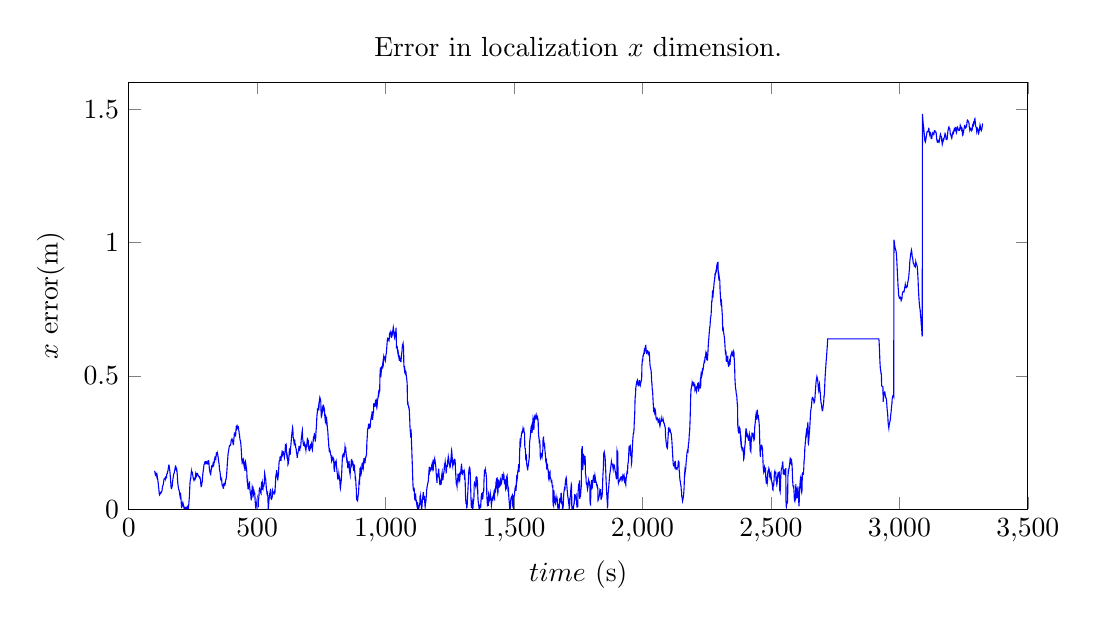
\begin{tikzpicture}

\begin{axis}[
title={Error in localization $x$ dimension.},
xlabel={$time$ (s)},
ylabel={$x$ error(m)},
xmin=0, xmax=3500,
ymin=0, ymax=1.6,
axis on top,
width=13cm,
height=7cm
]
\addplot [blue]
coordinates {
(100,0.143275262832641)
(101,0.142355205535889)
(102,0.139847995758057)
(103,0.131320001602173)
(104,0.128383399963379)
(105,0.130818759918213)
(106,0.132640516281128)
(107,0.130444919586182)
(108,0.129468460083008)
(109,0.124511499404907)
(110,0.129545230865479)
(111,0.124238033294678)
(112,0.112614715576172)
(113,0.112366998672485)
(114,0.103152359008789)
(115,0.0973518142700196)
(116,0.0834021816253663)
(117,0.0781326541900635)
(118,0.0683923015594483)
(119,0.0573310604095458)
(120,0.0530957927703857)
(121,0.0547282447814941)
(122,0.0567631473541259)
(123,0.0608091106414794)
(124,0.0629060020446777)
(125,0.0635807266235351)
(126,0.0614442787170413)
(127,0.0629486999511721)
(128,0.0639705619812014)
(129,0.0669399242401125)
(130,0.0725615959167483)
(131,0.0808940868377688)
(132,0.0869217853546145)
(133,0.0879730587005616)
(134,0.0906967525482179)
(135,0.0961598758697511)
(136,0.100356281280518)
(137,0.111034572601318)
(138,0.112635791778565)
(139,0.115686595916748)
(140,0.116062696456909)
(141,0.115782554626465)
(142,0.114190156936646)
(143,0.11204224395752)
(144,0.120351022720337)
(145,0.121593898773193)
(146,0.116976684570313)
(147,0.117845672607422)
(148,0.128982919692993)
(149,0.132676738739014)
(150,0.133206981658935)
(151,0.138474424362183)
(152,0.142013032913208)
(153,0.144649465560913)
(154,0.152787168502808)
(155,0.156381567001343)
(156,0.1650068359375)
(157,0.164885957717896)
(158,0.156808721542359)
(159,0.150277006149292)
(160,0.143442737579346)
(161,0.135041408538819)
(162,0.121772699356079)
(163,0.110362224578858)
(164,0.0956298637390138)
(165,0.0795758571624758)
(166,0.0776482429504397)
(167,0.0773099269866946)
(168,0.0816830005645754)
(169,0.0845146980285647)
(170,0.095107397079468)
(171,0.102739175796509)
(172,0.112016042709351)
(173,0.118003448486328)
(174,0.124567111968994)
(175,0.131828149795532)
(176,0.133084903717041)
(177,0.134485136032104)
(178,0.142000804901123)
(179,0.144048673629761)
(180,0.150568706512451)
(181,0.15648673248291)
(182,0.161143047332764)
(183,0.160388208389282)
(184,0.155041433334351)
(185,0.148153997421265)
(186,0.145379043579102)
(187,0.14822380065918)
(188,0.141851825714111)
(189,0.130198163986206)
(190,0.111832509994507)
(191,0.0990501747131347)
(192,0.0894662246704101)
(193,0.0821236934661864)
(194,0.0781294670104979)
(195,0.0725883808135985)
(196,0.0704786148071288)
(197,0.0673062286376953)
(198,0.0619317970275879)
(199,0.0528258762359619)
(200,0.0476951637268068)
(201,0.0527651348114015)
(202,0.0551927127838137)
(203,0.0464892425537111)
(204,0.0339210357666015)
(205,0.0152433242797851)
(206,0.00381782913208006)
(207,0.0166479930877683)
(208,0.0233356342315671)
(209,0.0235158786773679)
(210,0.019274173736572)
(211,0.0241135807037351)
(212,0.0202430934906004)
(213,0.0162588806152342)
(214,0.00992123794555644)
(215,0.00496736717224122)
(216,0.00651828002929689)
(217,0.00281826210021974)
(218,0.00323850440979001)
(219,0.00436193275451657)
(220,0.0034610576629639)
(221,0.00483908271789568)
(222,0.00311317062377947)
(223,0.00473250961303728)
(224,0.00221862411499041)
(225,0.00331865310668933)
(226,0.000582323074340696)
(227,0.00702704429626477)
(228,0.00884573936462418)
(229,0.00307243347167985)
(230,0.00159341812133773)
(231,0.00189023590087878)
(232,0.000685506820678583)
(233,0.0065782604217528)
(234,0.0211432514190673)
(235,0.0334355430603028)
(236,0.0446538524627687)
(237,0.0649926261901856)
(238,0.0887876129150391)
(239,0.10344916343689)
(240,0.111184892654419)
(241,0.111450729370117)
(242,0.122715768814087)
(243,0.133800563812256)
(244,0.14280348777771)
(245,0.137242942810059)
(246,0.137228876113892)
(247,0.13514605140686)
(248,0.136347242355347)
(249,0.129933782577515)
(250,0.123188444137573)
(251,0.117756792068481)
(252,0.113195606231689)
(253,0.112652488708496)
(254,0.108656831741333)
(255,0.112222620010376)
(256,0.109344430923462)
(257,0.10973233795166)
(258,0.110864349365234)
(259,0.11481273651123)
(260,0.123825435638428)
(261,0.132441883087158)
(262,0.128805999755859)
(263,0.121950750350952)
(264,0.123841409683227)
(265,0.132286672592163)
(266,0.134263189315796)
(267,0.133845003128052)
(268,0.131576927185058)
(269,0.130946992874145)
(270,0.126172422409057)
(271,0.12601506614685)
(272,0.1255296459198)
(273,0.122076240539551)
(274,0.121950593948364)
(275,0.119712320327759)
(276,0.121587108612061)
(277,0.121123861312866)
(278,0.11342723274231)
(279,0.113496145248413)
(280,0.104672988891602)
(281,0.0895231571197512)
(282,0.085255506515503)
(283,0.0865353374481201)
(284,0.088600757598877)
(285,0.0984436302185059)
(286,0.100861875534058)
(287,0.111787168502808)
(288,0.126788942337036)
(289,0.137350873947144)
(290,0.141997890472412)
(291,0.150584774017334)
(292,0.157486169815063)
(293,0.167214363098144)
(294,0.168275564193725)
(295,0.170768707275391)
(296,0.174358575820923)
(297,0.172713487625122)
(298,0.175871580123901)
(299,0.178417587280273)
(300,0.178771162033081)
(301,0.173528814315796)
(302,0.176243686676025)
(303,0.177175745010376)
(304,0.176547988891602)
(305,0.175164445877075)
(306,0.169451221466065)
(307,0.169540811538696)
(308,0.173741508483887)
(309,0.181889940261841)
(310,0.182241130828857)
(311,0.181777883529663)
(312,0.177723575592041)
(313,0.162474653244018)
(314,0.152527591705322)
(315,0.145656606674194)
(316,0.139848932266236)
(317,0.135265573501587)
(318,0.13213084602356)
(319,0.130313003540039)
(320,0.137548530578613)
(321,0.145026529312134)
(322,0.155692249298096)
(323,0.161897808074951)
(324,0.161433130264282)
(325,0.157770544052124)
(326,0.159711528778076)
(327,0.164576936721802)
(328,0.169270683288574)
(329,0.161193660736084)
(330,0.16145997428894)
(331,0.166355899810791)
(332,0.172526887893677)
(333,0.175125116348267)
(334,0.18785666847229)
(335,0.18943833732605)
(336,0.195050973892212)
(337,0.194275636672974)
(338,0.193119068145752)
(339,0.189021368026733)
(340,0.199180593490601)
(341,0.206943264007569)
(342,0.205249061584473)
(343,0.209936100959778)
(344,0.20912094783783)
(345,0.211696822166443)
(346,0.206623513221741)
(347,0.202005464553833)
(348,0.194300491333008)
(349,0.190046388626099)
(350,0.179334241867065)
(351,0.174737531661987)
(352,0.167500812530518)
(353,0.155758188247681)
(354,0.143984363555908)
(355,0.142407224655151)
(356,0.135682867050171)
(357,0.124428682327271)
(358,0.112392120361328)
(359,0.109284711837768)
(360,0.107779098510742)
(361,0.106548620223999)
(362,0.110294414520264)
(363,0.0952067260742187)
(364,0.089716661453247)
(365,0.0904667263031005)
(366,0.0889421176910399)
(367,0.0833950710296629)
(368,0.0785771083831786)
(369,0.0784658451080325)
(370,0.0931042690277102)
(371,0.0955971736907961)
(372,0.0931093978881838)
(373,0.0930099773406985)
(374,0.0902068901062014)
(375,0.0914869594573977)
(376,0.0976057109832764)
(377,0.105529790878296)
(378,0.111027723312378)
(379,0.111606603622437)
(380,0.119278198242188)
(381,0.127009159088135)
(382,0.141506677627564)
(383,0.155196382522583)
(384,0.172715379714966)
(385,0.18186946105957)
(386,0.196978046417236)
(387,0.20937465763092)
(388,0.214157095909119)
(389,0.218686333656311)
(390,0.225435005187988)
(391,0.232325421333313)
(392,0.238009081840515)
(393,0.238707701683044)
(394,0.238467137336731)
(395,0.239898840904236)
(396,0.23939773273468)
(397,0.2429192943573)
(398,0.249863831520081)
(399,0.257966129302979)
(400,0.257714836120606)
(401,0.261592237472534)
(402,0.263750164031983)
(403,0.260878293037415)
(404,0.25569960308075)
(405,0.252374021530152)
(406,0.246963196754455)
(407,0.242957168579101)
(408,0.244163208961487)
(409,0.259265237808227)
(410,0.268322114944458)
(411,0.280031328201294)
(412,0.288094644546509)
(413,0.275310383796692)
(414,0.275866733551025)
(415,0.28081201171875)
(416,0.271833168029785)
(417,0.287125574111939)
(418,0.301159606933594)
(419,0.313760624885559)
(420,0.295252358436584)
(421,0.308168327331543)
(422,0.311379110336304)
(423,0.306834494590759)
(424,0.305378875732422)
(425,0.307384572029114)
(426,0.3041162109375)
(427,0.305534753799439)
(428,0.297996315956116)
(429,0.2941632604599)
(430,0.284143569946289)
(431,0.281482222557068)
(432,0.271850946426392)
(433,0.262713792800903)
(434,0.258775833129883)
(435,0.25517297077179)
(436,0.24769747543335)
(437,0.238537638664245)
(438,0.225391238212585)
(439,0.207392304420471)
(440,0.189296724319458)
(441,0.180009605407715)
(442,0.184358360290527)
(443,0.182991983413696)
(444,0.178225351333618)
(445,0.185863328933716)
(446,0.187850786209106)
(447,0.183799028396606)
(448,0.171228885650635)
(449,0.161786317825317)
(450,0.163106083869934)
(451,0.167127381324768)
(452,0.150091539382935)
(453,0.14345062828064)
(454,0.163249368667603)
(455,0.175347919464111)
(456,0.170747156143189)
(457,0.159895874023438)
(458,0.154635883331299)
(459,0.149252868652344)
(460,0.137085414886475)
(461,0.103483058929443)
(462,0.0995791931152343)
(463,0.102481462478638)
(464,0.0774024810791016)
(465,0.0760866489410401)
(466,0.0770353164672852)
(467,0.0869151439666749)
(468,0.0913360919952395)
(469,0.091677745819092)
(470,0.103837093353272)
(471,0.0803439750671386)
(472,0.0732996597290039)
(473,0.0616243019104004)
(474,0.0582781467437745)
(475,0.0557587776184083)
(476,0.0429044399261476)
(477,0.0326920185089112)
(478,0.0594900856018068)
(479,0.0561057338714601)
(480,0.0528737316131593)
(481,0.0832292938232424)
(482,0.0792889499664309)
(483,0.075230350494385)
(484,0.0776352787017824)
(485,0.0660872364044192)
(486,0.0563163661956789)
(487,0.0615041160583498)
(488,0.0660931968688967)
(489,0.0619022750854494)
(490,0.0613365077972414)
(491,0.0556614303588869)
(492,0.0332107849121095)
(493,0.0217292613983155)
(494,0.0111592121124269)
(495,0.00223078155517564)
(496,0.00758256340026842)
(497,0.0196303310394286)
(498,0.0192264652252199)
(499,0.0297848320007326)
(500,0.0375951862335206)
(501,0.0411690807342531)
(502,0.0174317131042478)
(503,0.0128569374084471)
(504,0.00639579391479472)
(505,0.0311244812011719)
(506,0.0394798603057862)
(507,0.0499552574157716)
(508,0.0685082759857178)
(509,0.0767434215545655)
(510,0.0746062374114991)
(511,0.074507532119751)
(512,0.0675900592803957)
(513,0.0671449317932131)
(514,0.061301769256592)
(515,0.0590637340545657)
(516,0.0840993671417238)
(517,0.0942891387939455)
(518,0.103359296798706)
(519,0.0721616401672365)
(520,0.0893058433532716)
(521,0.0967573776245119)
(522,0.085389820098877)
(523,0.0794560585021973)
(524,0.0868954334259033)
(525,0.0863892707824707)
(526,0.0865144100189208)
(527,0.093139585494995)
(528,0.0980574455261229)
(529,0.135777589797974)
(530,0.131605264663696)
(531,0.120480892181396)
(532,0.116057512283325)
(533,0.115090259552002)
(534,0.102713712692261)
(535,0.0888332214355469)
(536,0.0746833400726317)
(537,0.0711051540374754)
(538,0.0615395622253416)
(539,0.0514620857238768)
(540,0.0666857528686524)
(541,0.0534044075012208)
(542,0.0421095657348634)
(543,0.000598194122314322)
(544,0.00934910583496107)
(545,0.0194656829833986)
(546,0.0345687847137452)
(547,0.042836263656616)
(548,0.0507550983428953)
(549,0.0590863971710203)
(550,0.0601423683166504)
(551,0.0689240398406983)
(552,0.0723517837524414)
(553,0.0702722969055176)
(554,0.0380731315612794)
(555,0.0485594959259035)
(556,0.0384579391479494)
(557,0.039901035308838)
(558,0.0424733333587648)
(559,0.0496452026367189)
(560,0.0647573852539063)
(561,0.0586514854431153)
(562,0.0578442001342774)
(563,0.0643709602355957)
(564,0.0645988883972168)
(565,0.064789384841919)
(566,0.064244836807251)
(567,0.0612258510589601)
(568,0.066369016647339)
(569,0.0581414299011231)
(570,0.0775738430023192)
(571,0.0919178199768065)
(572,0.112483568191528)
(573,0.129240579605102)
(574,0.130024774551392)
(575,0.136276348114014)
(576,0.146217926025391)
(577,0.121438283920288)
(578,0.127377290725708)
(579,0.119291563034058)
(580,0.123173732757568)
(581,0.117247476577759)
(582,0.12461389541626)
(583,0.133530511856079)
(584,0.151340618133545)
(585,0.171666606903076)
(586,0.180162176132202)
(587,0.181704267501831)
(588,0.182888973236084)
(589,0.19530390548706)
(590,0.195752132415771)
(591,0.183105821609497)
(592,0.183160657882691)
(593,0.182904596328735)
(594,0.199176902770996)
(595,0.19787036895752)
(596,0.206868047714234)
(597,0.214008207321167)
(598,0.211973020553589)
(599,0.207221576690674)
(600,0.213550397872925)
(601,0.211251598358154)
(602,0.212487083435059)
(603,0.206465822219849)
(604,0.204616346359253)
(605,0.199679174423218)
(606,0.193757572174072)
(607,0.200844621658325)
(608,0.21155915260315)
(609,0.219850635528565)
(610,0.239256202697754)
(611,0.23756676864624)
(612,0.240588485717773)
(613,0.242185890197754)
(614,0.214558973312378)
(615,0.204325332641602)
(616,0.197515859603882)
(617,0.201489967346191)
(618,0.193761152267456)
(619,0.187635463714599)
(620,0.167529144287109)
(621,0.17017201423645)
(622,0.184416570663452)
(623,0.184054805755615)
(624,0.199704362869263)
(625,0.214288665771484)
(626,0.227349950790405)
(627,0.208713874816894)
(628,0.205746755599975)
(629,0.206529722213745)
(630,0.233064933776856)
(631,0.235560699462891)
(632,0.247795864105225)
(633,0.260010286331177)
(634,0.272623310089111)
(635,0.281172523498535)
(636,0.290409336090088)
(637,0.297710266113281)
(638,0.305837240219116)
(639,0.300141658782959)
(640,0.272290361404419)
(641,0.265928161621094)
(642,0.263890874862671)
(643,0.252553833007812)
(644,0.246263963699341)
(645,0.251004440307617)
(646,0.261360866546631)
(647,0.247057806015015)
(648,0.244350324630737)
(649,0.244528661727905)
(650,0.230293766021728)
(651,0.230073228836059)
(652,0.224425092697143)
(653,0.2134449634552)
(654,0.211568752288818)
(655,0.201852718353271)
(656,0.192096153259277)
(657,0.203260822296143)
(658,0.207189245223999)
(659,0.210864706039429)
(660,0.217008996963501)
(661,0.21755592918396)
(662,0.2262760887146)
(663,0.237321067810059)
(664,0.223805255889892)
(665,0.223034925460815)
(666,0.221828527450561)
(667,0.23221481513977)
(668,0.234162218093872)
(669,0.233002788543701)
(670,0.239635213851929)
(671,0.25513528251648)
(672,0.26521919631958)
(673,0.274123891830444)
(674,0.279584499359131)
(675,0.291531892776489)
(676,0.295864196777344)
(677,0.265251401901245)
(678,0.26130390548706)
(679,0.248502973556518)
(680,0.241402809143066)
(681,0.239202920913696)
(682,0.238582555770874)
(683,0.24028987121582)
(684,0.24656540107727)
(685,0.242909490585327)
(686,0.235218822479248)
(687,0.235381267547607)
(688,0.229542158126831)
(689,0.233135364532471)
(690,0.223315139770508)
(691,0.231983085632324)
(692,0.234092136383056)
(693,0.235088876724243)
(694,0.247294239044189)
(695,0.259870819091797)
(696,0.268288663864136)
(697,0.254743968963623)
(698,0.249343549728394)
(699,0.259689723968506)
(700,0.231551822662353)
(701,0.226968225479126)
(702,0.220373567581177)
(703,0.22054522895813)
(704,0.227008974075317)
(705,0.222553407669067)
(706,0.225589429855347)
(707,0.232863603591919)
(708,0.244345365524292)
(709,0.235499320983886)
(710,0.239034114837646)
(711,0.247321306228637)
(712,0.243915019989013)
(713,0.238764701843261)
(714,0.225604234695434)
(715,0.222015319824219)
(716,0.230274377822876)
(717,0.250280920028687)
(718,0.252723756790161)
(719,0.269418302536011)
(720,0.269128423690796)
(721,0.271713596343994)
(722,0.276737075805664)
(723,0.27169132232666)
(724,0.27564001083374)
(725,0.270466327667236)
(726,0.253209806442261)
(727,0.262026048660278)
(728,0.266990400314331)
(729,0.289019422531128)
(730,0.301074819564819)
(731,0.314959125518799)
(732,0.338070474624634)
(733,0.352816425323486)
(734,0.359893404006958)
(735,0.377799354553223)
(736,0.370159229278564)
(737,0.372476657867431)
(738,0.379429897308349)
(739,0.385888879776001)
(740,0.370583837509155)
(741,0.38899118232727)
(742,0.401729707717895)
(743,0.41302526473999)
(744,0.419209604263306)
(745,0.416085605621338)
(746,0.41207540512085)
(747,0.408735160827637)
(748,0.401391153335571)
(749,0.35558869934082)
(750,0.345872426986694)
(751,0.347494150161743)
(752,0.361142583847046)
(753,0.359951444625854)
(754,0.368066259384155)
(755,0.38204736328125)
(756,0.386610860824585)
(757,0.385274047851563)
(758,0.378752584457398)
(759,0.38504111289978)
(760,0.381929273605347)
(761,0.378082866668701)
(762,0.37109338760376)
(763,0.353385482788086)
(764,0.344101940155029)
(765,0.333722625732422)
(766,0.338646549224853)
(767,0.343746322631836)
(768,0.335014719009399)
(769,0.323614019393921)
(770,0.32639541053772)
(771,0.332729000091553)
(772,0.322697061538696)
(773,0.309950965881348)
(774,0.299157041549682)
(775,0.292631525039673)
(776,0.277926582336426)
(777,0.2593892993927)
(778,0.253657955169678)
(779,0.233992258071899)
(780,0.227799335479736)
(781,0.216340700149536)
(782,0.217210147857666)
(783,0.221422288894653)
(784,0.218763206481933)
(785,0.212466571807861)
(786,0.204913948059082)
(787,0.201462123870849)
(788,0.199370477676391)
(789,0.187424255371094)
(790,0.180201602935791)
(791,0.183560920715332)
(792,0.191069913864136)
(793,0.186611400604248)
(794,0.185788379669189)
(795,0.188171611785889)
(796,0.19188116645813)
(797,0.189556346893311)
(798,0.188165412902832)
(799,0.153706815719604)
(800,0.149376180648804)
(801,0.139478233337402)
(802,0.15810924911499)
(803,0.166259826660156)
(804,0.176519454956054)
(805,0.17791110420227)
(806,0.173841775894165)
(807,0.169858993530273)
(808,0.174843849182129)
(809,0.159506855010986)
(810,0.151296911239624)
(811,0.1399400806427)
(812,0.133120143890381)
(813,0.121367300033569)
(814,0.113386953353882)
(815,0.113776052474976)
(816,0.114125360488892)
(817,0.120848526000977)
(818,0.132323373794556)
(819,0.124109615325928)
(820,0.114403356552124)
(821,0.116577495574951)
(822,0.112850297927857)
(823,0.084061361312866)
(824,0.0782024631500242)
(825,0.08675382232666)
(826,0.0962361049652101)
(827,0.104838724136353)
(828,0.115279550552368)
(829,0.133863563537598)
(830,0.154127235412598)
(831,0.176820154190064)
(832,0.196095581054688)
(833,0.194899230957031)
(834,0.205325275421143)
(835,0.206076055526733)
(836,0.202551275253296)
(837,0.20798769569397)
(838,0.207582145690918)
(839,0.203670650482178)
(840,0.211448406219482)
(841,0.219095443725586)
(842,0.233219598770142)
(843,0.22640426826477)
(844,0.224983055114746)
(845,0.226428825378418)
(846,0.211351274490356)
(847,0.201777576446533)
(848,0.192138790130615)
(849,0.182957019805908)
(850,0.186515893936157)
(851,0.179257955551147)
(852,0.173513975143432)
(853,0.153265892028808)
(854,0.170219360351562)
(855,0.172632394790649)
(856,0.16959023475647)
(857,0.169199705123901)
(858,0.180518627166748)
(859,0.145711904525757)
(860,0.140681987762451)
(861,0.13532186126709)
(862,0.12960053062439)
(863,0.151609308242798)
(864,0.155360109329223)
(865,0.156208879470825)
(866,0.179169815063477)
(867,0.183923166275024)
(868,0.185070913314819)
(869,0.173948448181152)
(870,0.179592769622803)
(871,0.17970506477356)
(872,0.177499216079712)
(873,0.169297782897949)
(874,0.157404510498047)
(875,0.150981037139892)
(876,0.14355119895935)
(877,0.159720643997193)
(878,0.156477436065674)
(879,0.159180387496948)
(880,0.138307943344116)
(881,0.135149850845337)
(882,0.11475528717041)
(883,0.116711273193359)
(884,0.106163873672485)
(885,0.0876840496063234)
(886,0.0741137409210206)
(887,0.0395585327148438)
(888,0.034995439529419)
(889,0.0331555633544922)
(890,0.032564889907837)
(891,0.0312206859588624)
(892,0.0404884929656983)
(893,0.052567970275879)
(894,0.0542335624694825)
(895,0.0678758735656739)
(896,0.0845322723388673)
(897,0.111711256027222)
(898,0.105308763504028)
(899,0.102173082351685)
(900,0.154404426574707)
(901,0.148254419326782)
(902,0.151326442718506)
(903,0.123141231536865)
(904,0.13182014465332)
(905,0.142483415603638)
(906,0.139884414672852)
(907,0.148619358062744)
(908,0.164390508651733)
(909,0.174497072219848)
(910,0.149513317108154)
(911,0.159576488494873)
(912,0.161657405853271)
(913,0.156542612075806)
(914,0.178592157363891)
(915,0.180929613113403)
(916,0.191017341613769)
(917,0.175703121185303)
(918,0.17852742767334)
(919,0.178190065383911)
(920,0.176812482833862)
(921,0.185381723403931)
(922,0.194469285964966)
(923,0.19452388381958)
(924,0.19783417892456)
(925,0.203536912918091)
(926,0.205290004730224)
(927,0.249717882156372)
(928,0.261684110641479)
(929,0.278541019439697)
(930,0.297290733337402)
(931,0.302093597412109)
(932,0.305801721572876)
(933,0.310079189300537)
(934,0.320396753311157)
(935,0.303051584243774)
(936,0.303335779190063)
(937,0.303860776901245)
(938,0.314173717498779)
(939,0.317461271286011)
(940,0.32016040802002)
(941,0.316405076980591)
(942,0.332365579605102)
(943,0.337852067947388)
(944,0.34382230758667)
(945,0.349142986297607)
(946,0.351656394958496)
(947,0.35976501083374)
(948,0.366896825790405)
(949,0.335001598358154)
(950,0.3446594581604)
(951,0.351798664093018)
(952,0.362815271377563)
(953,0.362404237747192)
(954,0.394307359695435)
(955,0.395305379867554)
(956,0.393872007369995)
(957,0.38872198677063)
(958,0.385423704147339)
(959,0.385787530899048)
(960,0.391817375183106)
(961,0.407060335159302)
(962,0.408333728790283)
(963,0.409872482299805)
(964,0.390903184890747)
(965,0.386316249847412)
(966,0.380624959945679)
(967,0.386318872451782)
(968,0.404753686904907)
(969,0.411144973754883)
(970,0.4143619556427)
(971,0.421498594284058)
(972,0.431109962463379)
(973,0.43750768661499)
(974,0.432213651657104)
(975,0.438444482803344)
(976,0.441269742965698)
(977,0.441752779006958)
(978,0.499192296981811)
(979,0.516837656021118)
(980,0.531236946105957)
(981,0.494424945831299)
(982,0.502675659179687)
(983,0.514631158828735)
(984,0.52739155960083)
(985,0.532874696731567)
(986,0.532329433441162)
(987,0.537081830978393)
(988,0.538281438827515)
(989,0.546187875747681)
(990,0.535562990188599)
(991,0.539407012939453)
(992,0.56356364440918)
(993,0.573167621612549)
(994,0.569471179962158)
(995,0.566822826385498)
(996,0.568152725219726)
(997,0.564471303939819)
(998,0.561314403533935)
(999,0.556769191741943)
(1000,0.561858474731445)
(1001,0.577734384536743)
(1002,0.579806718826294)
(1003,0.587208662033081)
(1004,0.597822742462158)
(1005,0.611990051269531)
(1006,0.625553684234619)
(1007,0.634862499237061)
(1008,0.638708190917969)
(1009,0.636461811065674)
(1010,0.632184104919434)
(1011,0.633529466629028)
(1012,0.637578767776489)
(1013,0.6399801197052)
(1014,0.636886161804199)
(1015,0.655021039962768)
(1016,0.65972027015686)
(1017,0.660773603439331)
(1018,0.663715927124023)
(1019,0.655809967041015)
(1020,0.655802337646484)
(1021,0.646624652862549)
(1022,0.64551243019104)
(1023,0.656727163314819)
(1024,0.663631050109863)
(1025,0.664792625427246)
(1026,0.662815420150757)
(1027,0.658169357299804)
(1028,0.668637601852417)
(1029,0.674072114944458)
(1030,0.681252090454101)
(1031,0.674738733291626)
(1032,0.664576379776001)
(1033,0.659288494110107)
(1034,0.648715106964111)
(1035,0.644043771743774)
(1036,0.650762168884277)
(1037,0.659953443527221)
(1038,0.658944217681884)
(1039,0.65430673789978)
(1040,0.671662656784057)
(1041,0.680882541656494)
(1042,0.609722747802734)
(1043,0.611917390823364)
(1044,0.611867561340332)
(1045,0.610408916473389)
(1046,0.597329286575317)
(1047,0.59155955696106)
(1048,0.599047092437744)
(1049,0.580729688644409)
(1050,0.582041229248047)
(1051,0.572982038497925)
(1052,0.567270959854126)
(1053,0.573268617630005)
(1054,0.573674882888794)
(1055,0.558344568252564)
(1056,0.558593238830567)
(1057,0.561561311721802)
(1058,0.558953012466431)
(1059,0.553379024505615)
(1060,0.553319896697998)
(1061,0.567011322021485)
(1062,0.575909818649292)
(1063,0.585897172927857)
(1064,0.593395437240601)
(1065,0.607745613098145)
(1066,0.617341245651245)
(1067,0.618086303710938)
(1068,0.621708358764649)
(1069,0.610320295333862)
(1070,0.608651603698731)
(1071,0.542139139175415)
(1072,0.53169807434082)
(1073,0.526801195144653)
(1074,0.519169284820557)
(1075,0.524472667694092)
(1076,0.516272022247314)
(1077,0.512101127624512)
(1078,0.517951681137085)
(1079,0.517006351470947)
(1080,0.504370643615723)
(1081,0.497660829544067)
(1082,0.490746213912964)
(1083,0.481179668426514)
(1084,0.471653415679932)
(1085,0.406050506591797)
(1086,0.39651233291626)
(1087,0.398257556915283)
(1088,0.389380517959595)
(1089,0.38790113067627)
(1090,0.380588117599487)
(1091,0.381011310577393)
(1092,0.375234666824341)
(1093,0.356149974822998)
(1094,0.335376564025879)
(1095,0.308505836486817)
(1096,0.294039789199829)
(1097,0.283047262191773)
(1098,0.268593851089478)
(1099,0.299309768676758)
(1100,0.279081144332886)
(1101,0.246159830093384)
(1102,0.223042423248291)
(1103,0.192514116287231)
(1104,0.168159420013428)
(1105,0.136318618774414)
(1106,0.10631491279602)
(1107,0.084209934234619)
(1108,0.0753400478363035)
(1109,0.0672385845184325)
(1110,0.0791589641571044)
(1111,0.0786530399322509)
(1112,0.069443883895874)
(1113,0.0396009140014648)
(1114,0.0371518783569336)
(1115,0.0446060352325439)
(1116,0.0509184055328369)
(1117,0.0531005115509031)
(1118,0.0371593685150144)
(1119,0.034397766113281)
(1120,0.0262614879608152)
(1121,0.0206760559082029)
(1122,0.0124630126953122)
(1123,0.00845710372924779)
(1124,0.0268507137298584)
(1125,0.0197458400726318)
(1126,0.00354291343688962)
(1127,0.00141445350646974)
(1128,0.00347176742553712)
(1129,0.00716344070434571)
(1130,0.00630530166625975)
(1131,0.0128994827270508)
(1132,0.0148764495849609)
(1133,0.0180805568695068)
(1134,0.0444330558776853)
(1135,0.0423118457794187)
(1136,0.0485455379486082)
(1137,0.0331658706665037)
(1138,0.0266496524810789)
(1139,0.0144416675567625)
(1140,0.000143112182617422)
(1141,0.00216125488281227)
(1142,0.014128694534302)
(1143,0.0352213478088381)
(1144,0.039561836242676)
(1145,0.0483039302825929)
(1146,0.0560210628509523)
(1147,0.0650258941650392)
(1148,0.0384017906188965)
(1149,0.0391685447692871)
(1150,0.0379025421142578)
(1151,0.0499516696929931)
(1152,0.0375934810638427)
(1153,0.0160361499786377)
(1154,0.00851343536376969)
(1155,0.0190760936737062)
(1156,0.0233921852111818)
(1157,0.0310100116729735)
(1158,0.0438421764373778)
(1159,0.055408815383911)
(1160,0.0722595252990721)
(1161,0.079479766845703)
(1162,0.0861123332977294)
(1163,0.0911217460632323)
(1164,0.0967783870697021)
(1165,0.099015230178833)
(1166,0.105118030548096)
(1167,0.116961711883545)
(1168,0.130594560623169)
(1169,0.144090482711792)
(1170,0.15609914970398)
(1171,0.155392808914184)
(1172,0.146820945739746)
(1173,0.15440408706665)
(1174,0.15314554977417)
(1175,0.152749298095703)
(1176,0.147536275863648)
(1177,0.150096176147461)
(1178,0.153031234741211)
(1179,0.159933929443359)
(1180,0.15617335319519)
(1181,0.164312644958496)
(1182,0.172704978942871)
(1183,0.16745619392395)
(1184,0.154094413757324)
(1185,0.146835521697998)
(1186,0.150042251586914)
(1187,0.185259944915771)
(1188,0.174802667617798)
(1189,0.182368404388427)
(1190,0.183649452209472)
(1191,0.188526065826416)
(1192,0.176529796600342)
(1193,0.178498418807983)
(1194,0.170316354751587)
(1195,0.162798063278198)
(1196,0.152853385925293)
(1197,0.132375734329224)
(1198,0.125537651062012)
(1199,0.112995164871216)
(1200,0.0983915500640871)
(1201,0.12320952796936)
(1202,0.120106510162354)
(1203,0.120899251937866)
(1204,0.127312568664551)
(1205,0.133638767242432)
(1206,0.144539503097534)
(1207,0.151375679016113)
(1208,0.127956583023071)
(1209,0.114797546386719)
(1210,0.104470922470093)
(1211,0.111054420471191)
(1212,0.106638193130493)
(1213,0.0939509868621826)
(1214,0.0922279148101808)
(1215,0.0920803337097169)
(1216,0.0951263694763185)
(1217,0.0997648029327394)
(1218,0.118190725326538)
(1219,0.131161172866821)
(1220,0.136344869613648)
(1221,0.110306537628174)
(1222,0.10981944847107)
(1223,0.111336029052735)
(1224,0.114316976547241)
(1225,0.133373403549194)
(1226,0.133713150024414)
(1227,0.138097906112671)
(1228,0.143285179138184)
(1229,0.171939609527588)
(1230,0.165396211624146)
(1231,0.168512580871582)
(1232,0.17700172996521)
(1233,0.167785182952881)
(1234,0.16159154510498)
(1235,0.14778338432312)
(1236,0.153025732040405)
(1237,0.147918567657471)
(1238,0.161752872467041)
(1239,0.161047153472901)
(1240,0.160562448501587)
(1241,0.171937875747681)
(1242,0.182249002456665)
(1243,0.18789475440979)
(1244,0.197045259475708)
(1245,0.190925628662109)
(1246,0.188962251663208)
(1247,0.172869235992432)
(1248,0.166379243850708)
(1249,0.167647319793701)
(1250,0.163882452011108)
(1251,0.15327520942688)
(1252,0.166747283935547)
(1253,0.174278211593628)
(1254,0.185302686691284)
(1255,0.183330488204956)
(1256,0.211486671447754)
(1257,0.220569227218628)
(1258,0.21509942817688)
(1259,0.188438938140869)
(1260,0.168170497894287)
(1261,0.162802026748657)
(1262,0.184377769470215)
(1263,0.181048015594482)
(1264,0.17229662322998)
(1265,0.169910291671753)
(1266,0.177355350494385)
(1267,0.181514085769653)
(1268,0.181394876480102)
(1269,0.186192831039429)
(1270,0.185394844055176)
(1271,0.174380382537842)
(1272,0.147765420913696)
(1273,0.13223745727539)
(1274,0.114650749206543)
(1275,0.0991206398010251)
(1276,0.101012937545776)
(1277,0.0911614818572999)
(1278,0.0854568405151368)
(1279,0.104485832214356)
(1280,0.108317218780518)
(1281,0.115519605636597)
(1282,0.132880054473877)
(1283,0.116307077407837)
(1284,0.112809715270996)
(1285,0.107411203384399)
(1286,0.122457864761353)
(1287,0.127394083023071)
(1288,0.120068910598755)
(1289,0.114764812469482)
(1290,0.126622510910034)
(1291,0.131970954895019)
(1292,0.136741949081421)
(1293,0.142317813873291)
(1294,0.155431550979614)
(1295,0.163761896133423)
(1296,0.170446437835693)
(1297,0.135291194915772)
(1298,0.131667947769165)
(1299,0.130892133712769)
(1300,0.148024333953857)
(1301,0.140617383956909)
(1302,0.138330234527588)
(1303,0.1386985912323)
(1304,0.139889862060547)
(1305,0.141692783355713)
(1306,0.130367185592651)
(1307,0.137856136322021)
(1308,0.130642782211304)
(1309,0.115811954498291)
(1310,0.0973311767578124)
(1311,0.0519236793518068)
(1312,0.0346900691986085)
(1313,0.0193752517700196)
(1314,0.0304521312713621)
(1315,0.0209766616821287)
(1316,0.00621163749694809)
(1317,0.00746524429321305)
(1318,0.0213798236846925)
(1319,0.0488120269775392)
(1320,0.0615795803070069)
(1321,0.0819457378387454)
(1322,0.100270112991333)
(1323,0.122590860366822)
(1324,0.141882976531983)
(1325,0.148632360458374)
(1326,0.155468297958374)
(1327,0.156864953994751)
(1328,0.154076162338257)
(1329,0.145678821563721)
(1330,0.122112575531006)
(1331,0.0870054893493655)
(1332,0.052179210662842)
(1333,0.0232690505981448)
(1334,0.00496208000183129)
(1335,0.0140562648773193)
(1336,0.0219898815155029)
(1337,0.026718198776245)
(1338,0.00341962432861331)
(1339,0.00353501892089847)
(1340,0.00355769538879391)
(1341,0.0190761165618896)
(1342,0.0301840381622314)
(1343,0.03288055229187)
(1344,0.045545347213745)
(1345,0.0921881790161132)
(1346,0.0977960224151611)
(1347,0.0939329261779784)
(1348,0.0916836853027343)
(1349,0.0890193519592284)
(1350,0.088591152191162)
(1351,0.084393793106079)
(1352,0.11938321685791)
(1353,0.120498300552368)
(1354,0.117710710525513)
(1355,0.111830097198486)
(1356,0.0999964294433595)
(1357,0.10565672492981)
(1358,0.0950864372253419)
(1359,0.0541585636138917)
(1360,0.0340512943267823)
(1361,0.0257221412658692)
(1362,0.0196384143829347)
(1363,0.00940459442138675)
(1364,0.0027020626068115)
(1365,0.00471932220458982)
(1366,0.00395598602294944)
(1367,0.0122543830871584)
(1368,0.014626647949219)
(1369,0.0116160583496092)
(1370,0.00384075164794906)
(1371,0.0218960571289064)
(1372,0.0438854026794435)
(1373,0.0502572536468509)
(1374,0.0581849098205569)
(1375,0.0590827941894534)
(1376,0.035853879928589)
(1377,0.0453407936096193)
(1378,0.0495894126892091)
(1379,0.0471050910949709)
(1380,0.0618142890930176)
(1381,0.0655107307434082)
(1382,0.0681645679473877)
(1383,0.106368312835694)
(1384,0.124581108093262)
(1385,0.14324499130249)
(1386,0.14120436668396)
(1387,0.141867166519165)
(1388,0.141350036621094)
(1389,0.146428113937378)
(1390,0.134515567779541)
(1391,0.134143396377564)
(1392,0.123613639831543)
(1393,0.113131090164185)
(1394,0.0542428436279296)
(1395,0.0366370620727539)
(1396,0.0218872966766357)
(1397,0.0267960529327391)
(1398,0.026481101989746)
(1399,0.0202834110260008)
(1400,0.0119821529388426)
(1401,0.0572606163024902)
(1402,0.0539890365600586)
(1403,0.0439742641448975)
(1404,0.0323051052093506)
(1405,0.0346677570343017)
(1406,0.0348732738494872)
(1407,0.0395267276763915)
(1408,0.0568285446166992)
(1409,0.0502791862487793)
(1410,0.0417764644622802)
(1411,0.0255799751281738)
(1412,0.0142863063812255)
(1413,0.021947410583496)
(1414,0.0354707508087158)
(1415,0.038731206893921)
(1416,0.0343030586242676)
(1417,0.0337301387786866)
(1418,0.0434011821746827)
(1419,0.0504018669128419)
(1420,0.0524110202789307)
(1421,0.0579895381927491)
(1422,0.0505735111236572)
(1423,0.0406245422363281)
(1424,0.0381797981262206)
(1425,0.0711125030517579)
(1426,0.075814832687378)
(1427,0.0761197700500489)
(1428,0.072312463760376)
(1429,0.0866767940521238)
(1430,0.0801016864776609)
(1431,0.0870329914093015)
(1432,0.114624378204346)
(1433,0.114951488494873)
(1434,0.116158124923706)
(1435,0.10844003868103)
(1436,0.0719887218475344)
(1437,0.0598782501220705)
(1438,0.0648998222351076)
(1439,0.108695697784424)
(1440,0.107785415649414)
(1441,0.102685880661011)
(1442,0.0945956230163576)
(1443,0.0901150226593019)
(1444,0.0856847286224367)
(1445,0.0876047134399416)
(1446,0.0943483829498293)
(1447,0.110676816940308)
(1448,0.106991104125977)
(1449,0.10381107711792)
(1450,0.0942155151367188)
(1451,0.0959588317871094)
(1452,0.103669288635254)
(1453,0.109122159957886)
(1454,0.131585678100586)
(1455,0.125216802597046)
(1456,0.115709146499634)
(1457,0.114507595062256)
(1458,0.122184911727905)
(1459,0.121641078948974)
(1460,0.129051128387451)
(1461,0.123808868408203)
(1462,0.104881055831909)
(1463,0.0927124099731444)
(1464,0.106319971084595)
(1465,0.108066148757934)
(1466,0.0931752395629881)
(1467,0.0803702545166014)
(1468,0.0864069156646727)
(1469,0.0800144367218016)
(1470,0.0788483314514159)
(1471,0.115852540969849)
(1472,0.123831695556641)
(1473,0.125932640075683)
(1474,0.110740127563477)
(1475,0.094297113418579)
(1476,0.0825976753234863)
(1477,0.0638181591033935)
(1478,0.0836118125915526)
(1479,0.0591452980041502)
(1480,0.0402493143081664)
(1481,0.0317546472549437)
(1482,0.0181906566619872)
(1483,0.00299492931365952)
(1484,0.00740245437622056)
(1485,0.00389019107818589)
(1486,0.0113716974258424)
(1487,0.0312002553939821)
(1488,0.039656843185425)
(1489,0.0383557929992677)
(1490,0.0397288370132447)
(1491,0.047593789100647)
(1492,0.0490101146697999)
(1493,0.0515094566345216)
(1494,0.0207973976135254)
(1495,0.0123336572647095)
(1496,0.00716879558563233)
(1497,0.00547858333587659)
(1498,0.0276856050491334)
(1499,0.0517590866088868)
(1500,0.0448881072998046)
(1501,0.0503735227584838)
(1502,0.056996314048767)
(1503,0.0676670246124269)
(1504,0.0783393554687501)
(1505,0.0814823083877565)
(1506,0.0763346557617188)
(1507,0.0750041608810426)
(1508,0.0690439348220826)
(1509,0.102416086196899)
(1510,0.114403295516968)
(1511,0.129487562179565)
(1512,0.111904479980469)
(1513,0.118429877281189)
(1514,0.133257247924805)
(1515,0.144164778709412)
(1516,0.144098334312439)
(1517,0.156055264472961)
(1518,0.168743185997009)
(1519,0.138719519615173)
(1520,0.150792678833008)
(1521,0.184018811225891)
(1522,0.216265501976013)
(1523,0.245130124092102)
(1524,0.265573682785034)
(1525,0.231634594917297)
(1526,0.247782685279846)
(1527,0.263016082763672)
(1528,0.273494817733765)
(1529,0.282099418640137)
(1530,0.284522705078125)
(1531,0.290355138778686)
(1532,0.291016172409058)
(1533,0.289385627746582)
(1534,0.296740960121155)
(1535,0.303305100440979)
(1536,0.298988282203674)
(1537,0.299881517410278)
(1538,0.301032125473023)
(1539,0.288759816169739)
(1540,0.287503588676453)
(1541,0.283740985870361)
(1542,0.23205889415741)
(1543,0.227404725074768)
(1544,0.226998936653137)
(1545,0.206025254249573)
(1546,0.182418927192688)
(1547,0.19412659072876)
(1548,0.205201729774475)
(1549,0.175940210342407)
(1550,0.164357716560364)
(1551,0.158977801322937)
(1552,0.166853005409241)
(1553,0.145834380149841)
(1554,0.15698032951355)
(1555,0.161298209190369)
(1556,0.164902582168579)
(1557,0.178122653961182)
(1558,0.181310906410217)
(1559,0.191808476448059)
(1560,0.229556597709656)
(1561,0.254820860862732)
(1562,0.260979808807373)
(1563,0.270052309036255)
(1564,0.279471392631531)
(1565,0.29301094532013)
(1566,0.30324258518219)
(1567,0.31080295753479)
(1568,0.31054022026062)
(1569,0.314033767700195)
(1570,0.286060587882996)
(1571,0.295094863891602)
(1572,0.309188858985901)
(1573,0.327381713867188)
(1574,0.340608580589294)
(1575,0.335078938484192)
(1576,0.335760219573975)
(1577,0.297561935424805)
(1578,0.311759523391724)
(1579,0.336304835319519)
(1580,0.343910864830017)
(1581,0.339608390808106)
(1582,0.344638069152832)
(1583,0.346758563995361)
(1584,0.344104724884033)
(1585,0.353288370132446)
(1586,0.355248886108398)
(1587,0.344140487670898)
(1588,0.340041958808899)
(1589,0.340558015823364)
(1590,0.349211537361145)
(1591,0.33298414516449)
(1592,0.34182875919342)
(1593,0.3375405626297)
(1594,0.327405746459961)
(1595,0.288630103111267)
(1596,0.273743127822876)
(1597,0.26850900554657)
(1598,0.255441072463989)
(1599,0.258706095695496)
(1600,0.256602528572083)
(1601,0.241141679763794)
(1602,0.198077438354492)
(1603,0.194000480651856)
(1604,0.204267499923706)
(1605,0.203837471008301)
(1606,0.207585411071777)
(1607,0.206690030097961)
(1608,0.200356798171997)
(1609,0.195144675254822)
(1610,0.201540253639221)
(1611,0.213904998779297)
(1612,0.222761891365051)
(1613,0.261831647872925)
(1614,0.268170721054077)
(1615,0.269319183349609)
(1616,0.244937059402466)
(1617,0.248543736457825)
(1618,0.245689150810242)
(1619,0.24410533618927)
(1620,0.221305193901062)
(1621,0.216097536087036)
(1622,0.201960625648498)
(1623,0.1943705701828)
(1624,0.172501224517822)
(1625,0.179967540740967)
(1626,0.182094472885132)
(1627,0.155034573554993)
(1628,0.157220275878906)
(1629,0.168025644302368)
(1630,0.168398054122925)
(1631,0.152923017501831)
(1632,0.148000269889832)
(1633,0.1467958984375)
(1634,0.122635610580444)
(1635,0.114046938896179)
(1636,0.110024579048157)
(1637,0.115190871238708)
(1638,0.137465086936951)
(1639,0.139231649398804)
(1640,0.140547719955444)
(1641,0.116434741020203)
(1642,0.116816449165344)
(1643,0.115602660179138)
(1644,0.109282302856445)
(1645,0.10412872505188)
(1646,0.105866200447083)
(1647,0.106566555023193)
(1648,0.0961015291213989)
(1649,0.085044919013977)
(1650,0.0822868928909302)
(1651,0.0839450941085815)
(1652,0.0173392801284791)
(1653,0.0183442144393922)
(1654,0.0142136125564576)
(1655,0.0717388830184937)
(1656,0.0545527181625367)
(1657,0.0354971132278443)
(1658,0.0294077835083009)
(1659,0.0320017347335815)
(1660,0.0294338474273681)
(1661,0.024838448524475)
(1662,0.0360274438858033)
(1663,0.0288618927001953)
(1664,0.0328796033859253)
(1665,0.0314676885604859)
(1666,0.0322503652572632)
(1667,0.0428865756988526)
(1668,0.0376764144897461)
(1669,0.0187507476806641)
(1670,0.00895318412780766)
(1671,0.00400760746002193)
(1672,0.00717869377136227)
(1673,0.0103699560165404)
(1674,0.0144825572967529)
(1675,0.0110890264511108)
(1676,0.00239235115051262)
(1677,0.030215196609497)
(1678,0.0268785285949706)
(1679,0.0319479036331176)
(1680,0.0380219812393188)
(1681,0.0362879629135131)
(1682,0.0324186677932738)
(1683,0.058445435523987)
(1684,0.0587819633483888)
(1685,0.0399672803878786)
(1686,0.0206003007888795)
(1687,0.0292156286239624)
(1688,0.0156052656173706)
(1689,0.000108177185058622)
(1690,0.0169029150009155)
(1691,0.00290227794647224)
(1692,0.0257105913162232)
(1693,0.0473711576461793)
(1694,0.0616516780853271)
(1695,0.0682829332351684)
(1696,0.0767644357681274)
(1697,0.084202618598938)
(1698,0.0705124740600587)
(1699,0.0886922483444215)
(1700,0.103810608863831)
(1701,0.108636056900024)
(1702,0.114859497070313)
(1703,0.118529355049133)
(1704,0.112607633590698)
(1705,0.0936851377487182)
(1706,0.0844374771118164)
(1707,0.0703855628967285)
(1708,0.0594929161071778)
(1709,0.0504363479614258)
(1710,0.0439396800994873)
(1711,0.0367316904067994)
(1712,0.029026240348816)
(1713,0.0211666526794434)
(1714,0.0257753992080687)
(1715,0.00400480270385728)
(1716,0.00809923171997085)
(1717,0.0232215261459352)
(1718,0.040495509147644)
(1719,0.0477743091583251)
(1720,0.0578956546783447)
(1721,0.0725511302947999)
(1722,0.0834491243362427)
(1723,0.0934101333618165)
(1724,0.0899235000610352)
(1725,0.00117093658447276)
(1726,0.00585919952392588)
(1727,0.00959140396118174)
(1728,0.00919649219512952)
(1729,0.00586340045928968)
(1730,0.00321385478973402)
(1731,0.00283232116699206)
(1732,0.0140244045257567)
(1733,0.0146825590133666)
(1734,0.0266377010345458)
(1735,0.0257557907104491)
(1736,0.0562401342391967)
(1737,0.0485089349746703)
(1738,0.0497542972564697)
(1739,0.047585880279541)
(1740,0.0479708070755005)
(1741,0.0419351215362549)
(1742,0.0469648361206054)
(1743,0.0337671756744384)
(1744,0.0202453851699829)
(1745,0.00581367015838619)
(1746,0.0182067432403565)
(1747,0.0138927974700929)
(1748,0.00730171585083017)
(1749,0.0554425096511841)
(1750,0.0716753578186036)
(1751,0.0854466533660889)
(1752,0.0926476097106934)
(1753,0.092208800315857)
(1754,0.0979382371902466)
(1755,0.108126578330994)
(1756,0.0384526262283325)
(1757,0.0496630678176879)
(1758,0.0512120733261108)
(1759,0.0504177818298339)
(1760,0.0675793895721435)
(1761,0.0772113809585571)
(1762,0.0900632152557372)
(1763,0.2127414894104)
(1764,0.226405735015869)
(1765,0.228338356018066)
(1766,0.235848660469055)
(1767,0.146959442138672)
(1768,0.158777374267578)
(1769,0.168667334556579)
(1770,0.183998126029968)
(1771,0.183542116165161)
(1772,0.199987276077271)
(1773,0.19790695476532)
(1774,0.18272346496582)
(1775,0.188287558555603)
(1776,0.199156346321106)
(1777,0.186489405632019)
(1778,0.134598323822021)
(1779,0.128183075904846)
(1780,0.124261805534363)
(1781,0.0987801485061646)
(1782,0.0951379470825195)
(1783,0.0960205726623535)
(1784,0.0909761123657227)
(1785,0.0830686025619507)
(1786,0.0746487312316895)
(1787,0.0794198446273804)
(1788,0.0842010908126831)
(1789,0.103844039916992)
(1790,0.10840105342865)
(1791,0.0984328918457031)
(1792,0.0958183937072754)
(1793,0.0940329961776734)
(1794,0.0969420604705811)
(1795,0.087316029548645)
(1796,0.024364520072937)
(1797,0.0184315929412842)
(1798,0.0169145355224609)
(1799,0.0723220081329345)
(1800,0.0766059131622314)
(1801,0.0958222122192383)
(1802,0.109115478515625)
(1803,0.0843473615646362)
(1804,0.0792758407592773)
(1805,0.0817971172332763)
(1806,0.0973275718688964)
(1807,0.107930165290832)
(1808,0.113372903823852)
(1809,0.121198874473572)
(1810,0.118348756790161)
(1811,0.121187249183655)
(1812,0.114505926132202)
(1813,0.0982144832611083)
(1814,0.114491677284241)
(1815,0.125426506996155)
(1816,0.119175052642822)
(1817,0.109599924087524)
(1818,0.107410407066345)
(1819,0.101014947891235)
(1820,0.100616431236267)
(1821,0.0919314384460448)
(1822,0.0899847507476805)
(1823,0.0862900972366332)
(1824,0.0883409738540648)
(1825,0.0825813770294188)
(1826,0.079514718055725)
(1827,0.0326095228195191)
(1828,0.0346955661773682)
(1829,0.03962832736969)
(1830,0.0415052776336671)
(1831,0.0474597816467286)
(1832,0.0509995822906495)
(1833,0.0594602231979371)
(1834,0.0699159507751466)
(1835,0.0675838594436646)
(1836,0.0730566387176514)
(1837,0.07306498336792)
(1838,0.0447756032943727)
(1839,0.0474421958923341)
(1840,0.0510269384384157)
(1841,0.042704174041748)
(1842,0.0459489316940307)
(1843,0.0515384168624877)
(1844,0.065479824066162)
(1845,0.101766265869141)
(1846,0.127522744178772)
(1847,0.143914498329163)
(1848,0.157964982032776)
(1849,0.204206790924072)
(1850,0.212186422348023)
(1851,0.21481439113617)
(1852,0.206339683532715)
(1853,0.203419152259827)
(1854,0.197064939498901)
(1855,0.18716973400116)
(1856,0.165111485481262)
(1857,0.143261376380921)
(1858,0.116049471855164)
(1859,0.0938765439987184)
(1860,0.0745914611816407)
(1861,0.0559549961090089)
(1862,0.0366128120422364)
(1863,0.026224458694458)
(1864,0.00331636714935302)
(1865,0.0188100690841675)
(1866,0.0555340127944945)
(1867,0.0642051773071288)
(1868,0.073048599243164)
(1869,0.0871193485260009)
(1870,0.101520069122314)
(1871,0.112544425010681)
(1872,0.125571973800659)
(1873,0.132914073944092)
(1874,0.138375064849853)
(1875,0.146173974990845)
(1876,0.153000852584839)
(1877,0.162808200836182)
(1878,0.168139001846313)
(1879,0.177707454681396)
(1880,0.171389123916626)
(1881,0.170377752304077)
(1882,0.16710235786438)
(1883,0.167507192611694)
(1884,0.162016010284424)
(1885,0.156887149810791)
(1886,0.150484657287598)
(1887,0.15814715385437)
(1888,0.161850032806397)
(1889,0.166009006500244)
(1890,0.164036458969116)
(1891,0.161041444778442)
(1892,0.153349822998047)
(1893,0.147094434738159)
(1894,0.141172117233276)
(1895,0.137510246276855)
(1896,0.131916707992554)
(1897,0.124224481582642)
(1898,0.116602358818054)
(1899,0.115085778236389)
(1900,0.117284474372864)
(1901,0.219045543670654)
(1902,0.214239025115967)
(1903,0.215162777900696)
(1904,0.214027428627014)
(1905,0.105823317527771)
(1906,0.0991368684768676)
(1907,0.105173269271851)
(1908,0.102461496353149)
(1909,0.102603236198425)
(1910,0.105041423797607)
(1911,0.106572190284729)
(1912,0.112114110946655)
(1913,0.115077653884888)
(1914,0.111840764045715)
(1915,0.112605654716492)
(1916,0.115866744041443)
(1917,0.111219012260437)
(1918,0.116629683494568)
(1919,0.121187683105469)
(1920,0.121632929801941)
(1921,0.120442386627197)
(1922,0.114573044776916)
(1923,0.120842618942261)
(1924,0.12936918258667)
(1925,0.128181381225586)
(1926,0.1203493309021)
(1927,0.118009848594665)
(1928,0.11041097164154)
(1929,0.111187333106995)
(1930,0.116909021377563)
(1931,0.0997940244674682)
(1932,0.0987930240631103)
(1933,0.104908341407776)
(1934,0.0972002687454223)
(1935,0.0925736370086669)
(1936,0.114222045898438)
(1937,0.117462392807007)
(1938,0.122060771942139)
(1939,0.133502479553223)
(1940,0.139715906143189)
(1941,0.137804504394531)
(1942,0.136721607208252)
(1943,0.169060657501221)
(1944,0.171569536209106)
(1945,0.179673145294189)
(1946,0.191709468841553)
(1947,0.218260261535645)
(1948,0.213026258468628)
(1949,0.225142213821411)
(1950,0.232486221313477)
(1951,0.229972574234009)
(1952,0.231313440322876)
(1953,0.233935567855835)
(1954,0.208506649017334)
(1955,0.210615699768066)
(1956,0.208609169006348)
(1957,0.169229513168335)
(1958,0.174067026138306)
(1959,0.19447279548645)
(1960,0.213037019729614)
(1961,0.235255941390991)
(1962,0.255877717971802)
(1963,0.26717232131958)
(1964,0.281792863845825)
(1965,0.283020719528198)
(1966,0.288558706283569)
(1967,0.297563299179077)
(1968,0.324515592575073)
(1969,0.341148864746094)
(1970,0.362412702560425)
(1971,0.40814960861206)
(1972,0.423415788650513)
(1973,0.430321821212768)
(1974,0.453981790542602)
(1975,0.46097484588623)
(1976,0.468366060256958)
(1977,0.47279993057251)
(1978,0.479558382034302)
(1979,0.480354223251343)
(1980,0.482696924209595)
(1981,0.469843034744263)
(1982,0.469567184448242)
(1983,0.465825443267822)
(1984,0.469343786239624)
(1985,0.473438148498535)
(1986,0.475760583877563)
(1987,0.483218078613281)
(1988,0.469605056762695)
(1989,0.472667781829834)
(1990,0.476317493438721)
(1991,0.473216382980347)
(1992,0.466949073791504)
(1993,0.472414581298828)
(1994,0.476725435256958)
(1995,0.480672216415405)
(1996,0.484304046630859)
(1997,0.49598536491394)
(1998,0.541101243972778)
(1999,0.551882293701172)
(2000,0.564482954025268)
(2001,0.55644895362854)
(2002,0.574770706176758)
(2003,0.575286643981934)
(2004,0.581602149963379)
(2005,0.582995468139648)
(2006,0.586410814285278)
(2007,0.594082408905029)
(2008,0.590203088760376)
(2009,0.597175401687622)
(2010,0.5966451587677)
(2011,0.605587326049805)
(2012,0.613551698684692)
(2013,0.613999687194824)
(2014,0.596987648010254)
(2015,0.590413017272949)
(2016,0.58366696357727)
(2017,0.583388013839722)
(2018,0.591185894012451)
(2019,0.590351190567016)
(2020,0.593836631774902)
(2021,0.593107070922851)
(2022,0.587209787368774)
(2023,0.585623588562012)
(2024,0.576401796340942)
(2025,0.588592830657959)
(2026,0.589010778427124)
(2027,0.579586091995239)
(2028,0.561786670684814)
(2029,0.545310754776001)
(2030,0.534413833618164)
(2031,0.531994581222534)
(2032,0.52699875831604)
(2033,0.523191213607788)
(2034,0.51450777053833)
(2035,0.496194658279419)
(2036,0.477116641998291)
(2037,0.469874200820923)
(2038,0.449555025100708)
(2039,0.446191892623901)
(2040,0.432416543960571)
(2041,0.412660942077637)
(2042,0.393365312576294)
(2043,0.378472972869873)
(2044,0.365890670776367)
(2045,0.365637216567993)
(2046,0.36555305480957)
(2047,0.361963663101196)
(2048,0.380839363098145)
(2049,0.370571390151978)
(2050,0.370750204086304)
(2051,0.366462007522583)
(2052,0.3500842628479)
(2053,0.341864067077637)
(2054,0.337949472427368)
(2055,0.340499771118164)
(2056,0.339933288574219)
(2057,0.33956135559082)
(2058,0.341099393844605)
(2059,0.338365034103393)
(2060,0.332988218307495)
(2061,0.325719074249267)
(2062,0.326706853866577)
(2063,0.333307710647583)
(2064,0.335553375244141)
(2065,0.337284770965576)
(2066,0.319263906478882)
(2067,0.317029685974121)
(2068,0.311941595077515)
(2069,0.317131795883179)
(2070,0.328933515548706)
(2071,0.330144443511963)
(2072,0.332607307434082)
(2073,0.339342445373535)
(2074,0.331089586257935)
(2075,0.329115242004395)
(2076,0.330181360244751)
(2077,0.333327293395996)
(2078,0.332596302032471)
(2079,0.332264184951782)
(2080,0.338340393066406)
(2081,0.333412757873535)
(2082,0.329879156112671)
(2083,0.323073698043823)
(2084,0.321929050445557)
(2085,0.319756580352783)
(2086,0.313512636184692)
(2087,0.313438131332398)
(2088,0.307449056625366)
(2089,0.302096321105957)
(2090,0.268216384887695)
(2091,0.264455331802368)
(2092,0.251437438964844)
(2093,0.244576467514038)
(2094,0.240100046157837)
(2095,0.230897804260254)
(2096,0.229675193786621)
(2097,0.228309770584106)
(2098,0.241225336074829)
(2099,0.262930486679077)
(2100,0.27354178237915)
(2101,0.301679054260254)
(2102,0.304857412338257)
(2103,0.305365243911743)
(2104,0.295271867752075)
(2105,0.298153156280518)
(2106,0.295659536361694)
(2107,0.292662137985229)
(2108,0.295656051635742)
(2109,0.290866460800171)
(2110,0.286985006332397)
(2111,0.286178197860718)
(2112,0.282093639373779)
(2113,0.269606466293335)
(2114,0.262346620559692)
(2115,0.246496406555176)
(2116,0.230773416519165)
(2117,0.212196556091309)
(2118,0.194748888015747)
(2119,0.179965267181396)
(2120,0.16779972076416)
(2121,0.163644323348999)
(2122,0.164543714523315)
(2123,0.167537775039673)
(2124,0.170199241638183)
(2125,0.164237585067749)
(2126,0.172700277328491)
(2127,0.17880665397644)
(2128,0.178987613677978)
(2129,0.153566780090332)
(2130,0.15199107170105)
(2131,0.149689617156982)
(2132,0.150915195465088)
(2133,0.154736330032349)
(2134,0.154386808395386)
(2135,0.152224590301514)
(2136,0.156820858001709)
(2137,0.157425010681152)
(2138,0.158732736587524)
(2139,0.173052906036377)
(2140,0.179875730514526)
(2141,0.179220794677734)
(2142,0.176254629135132)
(2143,0.144457120895386)
(2144,0.138031024932861)
(2145,0.119909543991089)
(2146,0.108679671287537)
(2147,0.104838403701782)
(2148,0.0978790845870972)
(2149,0.091619047164917)
(2150,0.085320517539978)
(2151,0.0721285791397095)
(2152,0.0660217256546021)
(2153,0.0479125242233276)
(2154,0.0449610214233398)
(2155,0.0372996788024902)
(2156,0.0306507806777954)
(2157,0.0354481801986695)
(2158,0.0385548934936524)
(2159,0.0459412202835083)
(2160,0.0516188364028931)
(2161,0.0653128843307496)
(2162,0.0796176414489747)
(2163,0.11114949798584)
(2164,0.130548187255859)
(2165,0.143580862045288)
(2166,0.136977279663086)
(2167,0.145401561737061)
(2168,0.148501956939697)
(2169,0.160426700592041)
(2170,0.176076002120972)
(2171,0.18609959602356)
(2172,0.194297618865967)
(2173,0.208769474029541)
(2174,0.215178165435791)
(2175,0.218847665786743)
(2176,0.216376108169556)
(2177,0.214853328704834)
(2178,0.230502885818481)
(2179,0.246521276473999)
(2180,0.247903091430664)
(2181,0.257801992416382)
(2182,0.277966005325317)
(2183,0.286257555007934)
(2184,0.300292779922485)
(2185,0.323563863754272)
(2186,0.355994989395142)
(2187,0.3952841796875)
(2188,0.429487470626831)
(2189,0.449291233062744)
(2190,0.452627208709717)
(2191,0.459165361404419)
(2192,0.463537719726562)
(2193,0.47211882019043)
(2194,0.466019834518433)
(2195,0.46649547958374)
(2196,0.470528329849243)
(2197,0.467131404876709)
(2198,0.472084550857544)
(2199,0.470349102020264)
(2200,0.471992288589477)
(2201,0.465514694213867)
(2202,0.465982471466064)
(2203,0.466859851837158)
(2204,0.452269107818603)
(2205,0.457656175613403)
(2206,0.451008350372314)
(2207,0.450741010665894)
(2208,0.447350221633911)
(2209,0.451370674133301)
(2210,0.444939781188965)
(2211,0.453473735809326)
(2212,0.456920553207397)
(2213,0.456080127716064)
(2214,0.460411783218384)
(2215,0.470049854278564)
(2216,0.472512002944946)
(2217,0.472989555358887)
(2218,0.441091064453125)
(2219,0.44901895904541)
(2220,0.453227523803711)
(2221,0.454286024093628)
(2222,0.456058427810669)
(2223,0.465897247314453)
(2224,0.473605796813965)
(2225,0.461404867172241)
(2226,0.458814687728882)
(2227,0.465009517669678)
(2228,0.504081577301025)
(2229,0.500922054290772)
(2230,0.506774038314819)
(2231,0.501267045974731)
(2232,0.505197376251221)
(2233,0.50937971496582)
(2234,0.529611915588379)
(2235,0.516413921356201)
(2236,0.526867860794067)
(2237,0.528691762924194)
(2238,0.541460985183716)
(2239,0.546267980575561)
(2240,0.549627775192261)
(2241,0.55956339263916)
(2242,0.547499477386475)
(2243,0.569538175582886)
(2244,0.570747911453247)
(2245,0.5699270362854)
(2246,0.578525262832641)
(2247,0.586936193466186)
(2248,0.583405929565429)
(2249,0.584511714935303)
(2250,0.561411840438843)
(2251,0.560250980377197)
(2252,0.55938766670227)
(2253,0.562881929397583)
(2254,0.577132923126221)
(2255,0.591609460830688)
(2256,0.611974937438965)
(2257,0.627401573181152)
(2258,0.638145668029785)
(2259,0.649655086517334)
(2260,0.661972982406616)
(2261,0.673389656066894)
(2262,0.681503040313721)
(2263,0.687855703353882)
(2264,0.704130870819092)
(2265,0.71799681854248)
(2266,0.722295028686523)
(2267,0.727181703567505)
(2268,0.74526789855957)
(2269,0.768611700057984)
(2270,0.782278806686401)
(2271,0.782045871734619)
(2272,0.805428058624268)
(2273,0.820561677932739)
(2274,0.79226372718811)
(2275,0.805119495391846)
(2276,0.818469982147217)
(2277,0.827492456436157)
(2278,0.838898162841797)
(2279,0.850546102523804)
(2280,0.856974582672119)
(2281,0.861273025512695)
(2282,0.877963994979858)
(2283,0.876680587768555)
(2284,0.884371255874634)
(2285,0.884424900054932)
(2286,0.894335245132446)
(2287,0.897861455917358)
(2288,0.895870880126953)
(2289,0.911138252258301)
(2290,0.91546936416626)
(2291,0.911524967193603)
(2292,0.919533390045166)
(2293,0.924760240554809)
(2294,0.92527236366272)
(2295,0.885207860946655)
(2296,0.875503747940063)
(2297,0.866572587966919)
(2298,0.856925218582153)
(2299,0.868354640960693)
(2300,0.860576234817505)
(2301,0.85862716293335)
(2302,0.824885444641113)
(2303,0.805274801254273)
(2304,0.792352275848389)
(2305,0.77565731048584)
(2306,0.77954496383667)
(2307,0.781382455825806)
(2308,0.770086898803711)
(2309,0.75472225189209)
(2310,0.738417282104492)
(2311,0.725793018341065)
(2312,0.67816272354126)
(2313,0.680941968917847)
(2314,0.681431680679321)
(2315,0.672665744781494)
(2316,0.661788135528564)
(2317,0.656494289398193)
(2318,0.648885637283325)
(2319,0.644384294509888)
(2320,0.629480749130249)
(2321,0.616629987716675)
(2322,0.597740798950195)
(2323,0.585113912582397)
(2324,0.58609762763977)
(2325,0.587700038909912)
(2326,0.554989465713501)
(2327,0.561627754211426)
(2328,0.552894720077515)
(2329,0.563720115661621)
(2330,0.572934516906738)
(2331,0.57248295211792)
(2332,0.572461017608643)
(2333,0.545959251403809)
(2334,0.543053405761719)
(2335,0.536076324462891)
(2336,0.536690650939941)
(2337,0.545110164642334)
(2338,0.550405441284179)
(2339,0.541399326324463)
(2340,0.542048778533935)
(2341,0.544894065856933)
(2342,0.561609354019165)
(2343,0.572125043869018)
(2344,0.575707759857178)
(2345,0.578494157791138)
(2346,0.583492841720581)
(2347,0.585287418365478)
(2348,0.586089458465576)
(2349,0.594078388214111)
(2350,0.573395483016968)
(2351,0.581686250686646)
(2352,0.580433837890625)
(2353,0.577830068588257)
(2354,0.58521722984314)
(2355,0.591420642852783)
(2356,0.588248006820679)
(2357,0.568025840759277)
(2358,0.549136413574219)
(2359,0.524594320297241)
(2360,0.487959558486939)
(2361,0.471024925231934)
(2362,0.457442218780518)
(2363,0.450426036834717)
(2364,0.445074731826782)
(2365,0.433068687438965)
(2366,0.429931814193726)
(2367,0.424747640609741)
(2368,0.410444194793701)
(2369,0.395789319992065)
(2370,0.392246896743774)
(2371,0.313924236297607)
(2372,0.304299278259277)
(2373,0.293180866241455)
(2374,0.289885444641113)
(2375,0.29441611289978)
(2376,0.292252225875854)
(2377,0.303143724441528)
(2378,0.29896639251709)
(2379,0.302618249893189)
(2380,0.300503477096558)
(2381,0.277883941650391)
(2382,0.261835271835327)
(2383,0.250823194503784)
(2384,0.257886306762695)
(2385,0.244475500106812)
(2386,0.232195989608765)
(2387,0.227134124755859)
(2388,0.230569021224976)
(2389,0.231371776580811)
(2390,0.231452123641968)
(2391,0.220931829452514)
(2392,0.22244554901123)
(2393,0.213694871902466)
(2394,0.187237491607666)
(2395,0.189681043624878)
(2396,0.201810350418091)
(2397,0.207481851577759)
(2398,0.231343235015869)
(2399,0.240175928115845)
(2400,0.249397005081177)
(2401,0.27659245300293)
(2402,0.289210517883301)
(2403,0.300778825759888)
(2404,0.300494630813599)
(2405,0.29143710899353)
(2406,0.280852754592896)
(2407,0.269194086074829)
(2408,0.280686319351196)
(2409,0.277600229263306)
(2410,0.273075759887695)
(2411,0.266469657897949)
(2412,0.262312763214111)
(2413,0.26345693397522)
(2414,0.256104581832886)
(2415,0.271316347122192)
(2416,0.279421148300171)
(2417,0.27150279045105)
(2418,0.260862884521484)
(2419,0.231184595108032)
(2420,0.220534914016723)
(2421,0.218190305709839)
(2422,0.215768926620483)
(2423,0.260679370880127)
(2424,0.256742603302002)
(2425,0.262290842056274)
(2426,0.277508405685425)
(2427,0.273971466064453)
(2428,0.275187877655029)
(2429,0.284269956588745)
(2430,0.284873052597046)
(2431,0.281077428817749)
(2432,0.272819562911987)
(2433,0.265793367385864)
(2434,0.272310743331909)
(2435,0.276546964645386)
(2436,0.271812925338745)
(2437,0.308643983840942)
(2438,0.316066192626953)
(2439,0.324789928436279)
(2440,0.33656422996521)
(2441,0.348115133285523)
(2442,0.355291294097901)
(2443,0.349206071853638)
(2444,0.337593179702759)
(2445,0.337878328323364)
(2446,0.339237552642822)
(2447,0.372609634399414)
(2448,0.36264087677002)
(2449,0.347167987823486)
(2450,0.348854461669922)
(2451,0.349414268493652)
(2452,0.340881029129028)
(2453,0.331639209747314)
(2454,0.324512565612793)
(2455,0.305855358123779)
(2456,0.277208173751831)
(2457,0.230897060394287)
(2458,0.209636560440063)
(2459,0.195752254486084)
(2460,0.23908465385437)
(2461,0.226561479568482)
(2462,0.233104162216187)
(2463,0.240189723968506)
(2464,0.240145847320556)
(2465,0.23718063545227)
(2466,0.227594539642334)
(2467,0.2280543384552)
(2468,0.205504947662353)
(2469,0.183119350433349)
(2470,0.157896854400635)
(2471,0.149420835494995)
(2472,0.140707590103149)
(2473,0.145212930679321)
(2474,0.151137632369995)
(2475,0.157298368453979)
(2476,0.152066511154175)
(2477,0.145155099868775)
(2478,0.149612096786499)
(2479,0.150987771987915)
(2480,0.120387178421021)
(2481,0.107544523239136)
(2482,0.0976627883911134)
(2483,0.0982793388366701)
(2484,0.122240119934082)
(2485,0.112556987762451)
(2486,0.100049787521362)
(2487,0.106576019287109)
(2488,0.14155739402771)
(2489,0.143796144485473)
(2490,0.142500101089477)
(2491,0.14618620300293)
(2492,0.152650684356689)
(2493,0.149355262756348)
(2494,0.144856781005859)
(2495,0.126902292251587)
(2496,0.128697822570801)
(2497,0.120158622741699)
(2498,0.125528522491455)
(2499,0.131861396789551)
(2500,0.134838529586792)
(2501,0.121361204147339)
(2502,0.109464117050171)
(2503,0.106101461410522)
(2504,0.100641437530518)
(2505,0.0930536079406736)
(2506,0.0879969882965086)
(2507,0.0737242984771727)
(2508,0.0720684814453123)
(2509,0.0951476192474363)
(2510,0.0943598842620847)
(2511,0.0924182033538816)
(2512,0.105465421676636)
(2513,0.124059196472168)
(2514,0.138110157012939)
(2515,0.141369577407837)
(2516,0.133286472320556)
(2517,0.132746454238891)
(2518,0.133540864944458)
(2519,0.14015602684021)
(2520,0.107738182067871)
(2521,0.106612131118774)
(2522,0.101478740692138)
(2523,0.0922631473541258)
(2524,0.0957283229827879)
(2525,0.109383508682251)
(2526,0.125345870971679)
(2527,0.130083963394165)
(2528,0.134700939178467)
(2529,0.13314764213562)
(2530,0.132709190368652)
(2531,0.12634341430664)
(2532,0.134356185913086)
(2533,0.141836568832397)
(2534,0.0726465549468993)
(2535,0.0701824989318847)
(2536,0.0657414760589599)
(2537,0.0796393718719481)
(2538,0.112457038879394)
(2539,0.129200222015381)
(2540,0.145249368667602)
(2541,0.150070896148681)
(2542,0.152825345993042)
(2543,0.157495250701904)
(2544,0.160416831970215)
(2545,0.176092687606812)
(2546,0.176396194458008)
(2547,0.16124302482605)
(2548,0.133353605270386)
(2549,0.132390394210816)
(2550,0.139564170837402)
(2551,0.150347843170166)
(2552,0.128306894302368)
(2553,0.135476856231689)
(2554,0.141806154251098)
(2555,0.143516330718994)
(2556,0.136437683105469)
(2557,0.141016750335693)
(2558,0.153984336853027)
(2559,0.0122469158172609)
(2560,0.00862376976013168)
(2561,0.0191997795104979)
(2562,0.0205117969512938)
(2563,0.0211154727935789)
(2564,0.0262529163360594)
(2565,0.0290395526885985)
(2566,0.119561471939087)
(2567,0.132494010925293)
(2568,0.150518217086792)
(2569,0.143975534439087)
(2570,0.150318660736084)
(2571,0.155680932998657)
(2572,0.163307466506958)
(2573,0.16764048576355)
(2574,0.181794204711914)
(2575,0.189367570877075)
(2576,0.186782636642456)
(2577,0.180304565429688)
(2578,0.17582968711853)
(2579,0.186705389022827)
(2580,0.185778656005859)
(2581,0.176431217193604)
(2582,0.169891872406006)
(2583,0.151614465713501)
(2584,0.117029556274414)
(2585,0.10093320274353)
(2586,0.0878442611694337)
(2587,0.0842381801605225)
(2588,0.0813709583282471)
(2589,0.082856544494629)
(2590,0.0633078899383546)
(2591,0.0417001457214354)
(2592,0.0331685752868651)
(2593,0.0301952571868895)
(2594,0.0407027778625491)
(2595,0.0347241935729983)
(2596,0.0354072628021243)
(2597,0.0948042755126952)
(2598,0.0507521514892577)
(2599,0.0525202636718749)
(2600,0.0402467136383056)
(2601,0.071993854522705)
(2602,0.0690167217254638)
(2603,0.0579159526824951)
(2604,0.0416608123779296)
(2605,0.0854027214050292)
(2606,0.0619983615875244)
(2607,0.0526430549621582)
(2608,0.0386762561798095)
(2609,0.0103440227508544)
(2610,0.0237085876464844)
(2611,0.0581944046020508)
(2612,0.0785894451141358)
(2613,0.0912573394775391)
(2614,0.10308743095398)
(2615,0.115733390808106)
(2616,0.119311100006104)
(2617,0.0998981056213379)
(2618,0.0776529369354249)
(2619,0.0686709938049317)
(2620,0.0634918270111084)
(2621,0.0704944190979004)
(2622,0.119438255310059)
(2623,0.134788597106934)
(2624,0.13590415763855)
(2625,0.130329462051392)
(2626,0.130410047531128)
(2627,0.140425296783447)
(2628,0.154439302444458)
(2629,0.17971614074707)
(2630,0.186579019546509)
(2631,0.200613767623901)
(2632,0.22929363822937)
(2633,0.237205320358276)
(2634,0.252534442901611)
(2635,0.25607328414917)
(2636,0.274564790725708)
(2637,0.282162714004516)
(2638,0.269647258758545)
(2639,0.278774398803711)
(2640,0.287910360336304)
(2641,0.302843946456909)
(2642,0.306605115890503)
(2643,0.314778820037842)
(2644,0.326338544845581)
(2645,0.24798583984375)
(2646,0.245382070541382)
(2647,0.255834579467773)
(2648,0.266113996505737)
(2649,0.280532598495483)
(2650,0.289585828781128)
(2651,0.303577423095703)
(2652,0.317925930023193)
(2653,0.336545467376709)
(2654,0.357518434524536)
(2655,0.368568181991577)
(2656,0.374201059341431)
(2657,0.381461381912231)
(2658,0.387362718582153)
(2659,0.401270389556885)
(2660,0.412555932998657)
(2661,0.417307615280151)
(2662,0.419051885604858)
(2663,0.418175935745239)
(2664,0.414684772491455)
(2665,0.413769006729126)
(2666,0.408222675323486)
(2667,0.405788421630859)
(2668,0.399264097213745)
(2669,0.401201486587524)
(2670,0.403462171554565)
(2671,0.413241386413574)
(2672,0.42466402053833)
(2673,0.442204236984253)
(2674,0.45349645614624)
(2675,0.468831539154053)
(2676,0.478377819061279)
(2677,0.487388610839844)
(2678,0.489934921264648)
(2679,0.49676513671875)
(2680,0.493656158447266)
(2681,0.490288496017456)
(2682,0.485011577606201)
(2683,0.473505020141602)
(2684,0.462558507919312)
(2685,0.450061082839966)
(2686,0.444551467895508)
(2687,0.451946258544922)
(2688,0.460912704467773)
(2689,0.467151641845703)
(2690,0.455201148986816)
(2691,0.442501306533813)
(2692,0.437420845031738)
(2693,0.423409223556519)
(2694,0.409297466278076)
(2695,0.400680541992188)
(2696,0.395222187042236)
(2697,0.390655994415283)
(2698,0.382798433303833)
(2699,0.374547004699707)
(2700,0.369508028030396)
(2701,0.370475053787231)
(2702,0.372153282165527)
(2703,0.385200977325439)
(2704,0.390520811080933)
(2705,0.396862268447876)
(2706,0.410901546478271)
(2707,0.427144050598145)
(2708,0.427409887313843)
(2709,0.449685335159302)
(2710,0.474532842636108)
(2711,0.49641227722168)
(2712,0.510353326797485)
(2713,0.526373147964478)
(2714,0.538198232650757)
(2715,0.555696249008179)
(2716,0.564457416534424)
(2717,0.578359603881836)
(2718,0.592941522598267)
(2719,0.605350494384766)
(2720,0.621208429336548)
(2721,0.638477563858032)
(2722,0.638477563858032)
(2723,0.638477563858032)
(2724,0.638477563858032)
(2725,0.638477563858032)
(2726,0.638477563858032)
(2727,0.638477563858032)
(2728,0.638477563858032)
(2729,0.638477563858032)
(2730,0.638477563858032)
(2731,0.638477563858032)
(2732,0.638477563858032)
(2733,0.638477563858032)
(2734,0.638477563858032)
(2735,0.638477563858032)
(2736,0.638477563858032)
(2737,0.638477563858032)
(2738,0.638477563858032)
(2739,0.638477563858032)
(2740,0.638477563858032)
(2741,0.638477563858032)
(2742,0.638477563858032)
(2743,0.638477563858032)
(2744,0.638477563858032)
(2745,0.638477563858032)
(2746,0.638477563858032)
(2747,0.638477563858032)
(2748,0.638477563858032)
(2749,0.638477563858032)
(2750,0.638477563858032)
(2751,0.638477563858032)
(2752,0.638477563858032)
(2753,0.638477563858032)
(2754,0.638477563858032)
(2755,0.638477563858032)
(2756,0.638477563858032)
(2757,0.638477563858032)
(2758,0.638477563858032)
(2759,0.638477563858032)
(2760,0.638477563858032)
(2761,0.638477563858032)
(2762,0.638477563858032)
(2763,0.638477563858032)
(2764,0.638477563858032)
(2765,0.638477563858032)
(2766,0.638477563858032)
(2767,0.638477563858032)
(2768,0.638477563858032)
(2769,0.638477563858032)
(2770,0.638477563858032)
(2771,0.638477563858032)
(2772,0.638477563858032)
(2773,0.638477563858032)
(2774,0.638477563858032)
(2775,0.638477563858032)
(2776,0.638477563858032)
(2777,0.638477563858032)
(2778,0.638477563858032)
(2779,0.638477563858032)
(2780,0.638477563858032)
(2781,0.638477563858032)
(2782,0.638477563858032)
(2783,0.638477563858032)
(2784,0.638477563858032)
(2785,0.638477563858032)
(2786,0.638477563858032)
(2787,0.638477563858032)
(2788,0.638477563858032)
(2789,0.638477563858032)
(2790,0.638477563858032)
(2791,0.638477563858032)
(2792,0.638477563858032)
(2793,0.638477563858032)
(2794,0.638477563858032)
(2795,0.638477563858032)
(2796,0.638477563858032)
(2797,0.638477563858032)
(2798,0.638477563858032)
(2799,0.638477563858032)
(2800,0.638477563858032)
(2801,0.638477563858032)
(2802,0.638477563858032)
(2803,0.638477563858032)
(2804,0.638477563858032)
(2805,0.638477563858032)
(2806,0.638477563858032)
(2807,0.638477563858032)
(2808,0.638477563858032)
(2809,0.638477563858032)
(2810,0.638477563858032)
(2811,0.638477563858032)
(2812,0.638477563858032)
(2813,0.638477563858032)
(2814,0.638477563858032)
(2815,0.638477563858032)
(2816,0.638477563858032)
(2817,0.638477563858032)
(2818,0.638477563858032)
(2819,0.638477563858032)
(2820,0.638477563858032)
(2821,0.638477563858032)
(2822,0.638477563858032)
(2823,0.638477563858032)
(2824,0.638477563858032)
(2825,0.638477563858032)
(2826,0.638477563858032)
(2827,0.638477563858032)
(2828,0.638477563858032)
(2829,0.638477563858032)
(2830,0.638477563858032)
(2831,0.638477563858032)
(2832,0.638477563858032)
(2833,0.638477563858032)
(2834,0.638477563858032)
(2835,0.638477563858032)
(2836,0.638477563858032)
(2837,0.638477563858032)
(2838,0.638477563858032)
(2839,0.638477563858032)
(2840,0.638477563858032)
(2841,0.638477563858032)
(2842,0.638477563858032)
(2843,0.638477563858032)
(2844,0.638477563858032)
(2845,0.638477563858032)
(2846,0.638477563858032)
(2847,0.638477563858032)
(2848,0.638477563858032)
(2849,0.638477563858032)
(2850,0.638477563858032)
(2851,0.638477563858032)
(2852,0.638477563858032)
(2853,0.638477563858032)
(2854,0.638477563858032)
(2855,0.638477563858032)
(2856,0.638477563858032)
(2857,0.638477563858032)
(2858,0.638477563858032)
(2859,0.638477563858032)
(2860,0.638477563858032)
(2861,0.638477563858032)
(2862,0.638477563858032)
(2863,0.638477563858032)
(2864,0.638477563858032)
(2865,0.638477563858032)
(2866,0.638477563858032)
(2867,0.638477563858032)
(2868,0.638477563858032)
(2869,0.638477563858032)
(2870,0.638477563858032)
(2871,0.638477563858032)
(2872,0.638477563858032)
(2873,0.638477563858032)
(2874,0.638477563858032)
(2875,0.638477563858032)
(2876,0.638477563858032)
(2877,0.638477563858032)
(2878,0.638477563858032)
(2879,0.638477563858032)
(2880,0.638477563858032)
(2881,0.638477563858032)
(2882,0.638477563858032)
(2883,0.638477563858032)
(2884,0.638477563858032)
(2885,0.638477563858032)
(2886,0.638477563858032)
(2887,0.638477563858032)
(2888,0.638477563858032)
(2889,0.638477563858032)
(2890,0.638477563858032)
(2891,0.638477563858032)
(2892,0.638477563858032)
(2893,0.638477563858032)
(2894,0.638477563858032)
(2895,0.638477563858032)
(2896,0.638477563858032)
(2897,0.638477563858032)
(2898,0.638477563858032)
(2899,0.638477563858032)
(2900,0.638477563858032)
(2901,0.638477563858032)
(2902,0.638477563858032)
(2903,0.638477563858032)
(2904,0.638477563858032)
(2905,0.638477563858032)
(2906,0.638477563858032)
(2907,0.638477563858032)
(2908,0.638477563858032)
(2909,0.638477563858032)
(2910,0.638477563858032)
(2911,0.638477563858032)
(2912,0.638477563858032)
(2913,0.638477563858032)
(2914,0.638477563858032)
(2915,0.638477563858032)
(2916,0.638477563858032)
(2917,0.638477563858032)
(2918,0.638477563858032)
(2919,0.638477563858032)
(2920,0.638477563858032)
(2921,0.631552934646606)
(2922,0.610115766525269)
(2923,0.58983039855957)
(2924,0.560477733612061)
(2925,0.542079925537109)
(2926,0.526123523712158)
(2927,0.523420810699463)
(2928,0.513240575790405)
(2929,0.50721001625061)
(2930,0.507654905319214)
(2931,0.462614059448242)
(2932,0.461896419525146)
(2933,0.459964513778687)
(2934,0.459964513778687)
(2935,0.459964513778687)
(2936,0.459964513778687)
(2937,0.402593612670898)
(2938,0.414585590362549)
(2939,0.420575141906738)
(2940,0.432976245880127)
(2941,0.435009479522705)
(2942,0.437739372253418)
(2943,0.43925666809082)
(2944,0.435835599899292)
(2945,0.428361892700195)
(2946,0.426045417785645)
(2947,0.41808819770813)
(2948,0.416351318359375)
(2949,0.414544105529785)
(2950,0.408993005752563)
(2951,0.394411563873291)
(2952,0.380300283432007)
(2953,0.368961811065674)
(2954,0.360917091369629)
(2955,0.347809791564941)
(2956,0.329176664352417)
(2957,0.31771183013916)
(2958,0.310298442840576)
(2959,0.303898334503174)
(2960,0.313745498657227)
(2961,0.320085525512695)
(2962,0.323625802993774)
(2963,0.32826042175293)
(2964,0.331547021865845)
(2965,0.336492538452148)
(2966,0.349799871444702)
(2967,0.3568115234375)
(2968,0.366093873977661)
(2969,0.377513647079468)
(2970,0.389508008956909)
(2971,0.39369010925293)
(2972,0.41276741027832)
(2973,0.416735410690308)
(2974,0.422905921936035)
(2975,0.425306081771851)
(2976,0.426880836486816)
(2977,0.426572561264038)
(2978,0.423754930496216)
(2979,1.01013219642639)
(2980,1.00434744644165)
(2981,0.997178915023804)
(2982,0.987303617477417)
(2983,0.983062389373779)
(2984,0.977267864227295)
(2985,0.974982860565186)
(2986,0.970701101303101)
(2987,0.969212177276611)
(2988,0.961213710784912)
(2989,0.950203540802002)
(2990,0.932430150985718)
(2991,0.913295152664185)
(2992,0.893704774856567)
(2993,0.874421957015991)
(2994,0.854695919036865)
(2995,0.834021690368652)
(2996,0.824330451965332)
(2997,0.806533220291138)
(2998,0.798688772201538)
(2999,0.795799139022827)
(3000,0.790293815612793)
(3001,0.790436151504517)
(3002,0.794088247299194)
(3003,0.795147779464722)
(3004,0.79276526260376)
(3005,0.79291904258728)
(3006,0.787091377258301)
(3007,0.782052400588989)
(3008,0.784303548812866)
(3009,0.787852886199951)
(3010,0.789796474456787)
(3011,0.802251222610474)
(3012,0.809044721603394)
(3013,0.81404531288147)
(3014,0.814201000213623)
(3015,0.815993669509888)
(3016,0.816201332092285)
(3017,0.817160966873169)
(3018,0.815583112716675)
(3019,0.81906879234314)
(3020,0.825857522964478)
(3021,0.831662061691284)
(3022,0.835315587997437)
(3023,0.842483404159546)
(3024,0.836860301971436)
(3025,0.832882287979126)
(3026,0.82981622505188)
(3027,0.829919221878052)
(3028,0.832639577865601)
(3029,0.835855606079102)
(3030,0.838477495193481)
(3031,0.837151649475098)
(3032,0.846495512008667)
(3033,0.851655128479004)
(3034,0.855524662017822)
(3035,0.862070682525635)
(3036,0.866955402374268)
(3037,0.875322225570679)
(3038,0.888804796218872)
(3039,0.89806139755249)
(3040,0.918463829040527)
(3041,0.930980804443359)
(3042,0.939378622055054)
(3043,0.946108701705933)
(3044,0.958624961853027)
(3045,0.958940628051758)
(3046,0.965977313995361)
(3047,0.972069385528564)
(3048,0.96755659866333)
(3049,0.957893255233765)
(3050,0.947491291046143)
(3051,0.945218923568726)
(3052,0.938712480545044)
(3053,0.93175804901123)
(3054,0.924298170089722)
(3055,0.920703294754028)
(3056,0.921293142318726)
(3057,0.9198297290802)
(3058,0.912185075759888)
(3059,0.913457754135132)
(3060,0.911984088897705)
(3061,0.91179693031311)
(3062,0.90965545463562)
(3063,0.916745546340942)
(3064,0.927840116500855)
(3065,0.922645214080811)
(3066,0.91911065864563)
(3067,0.919447067260742)
(3068,0.91616499710083)
(3069,0.913457754135132)
(3070,0.906820896148682)
(3071,0.893299224853516)
(3072,0.875048759460449)
(3073,0.855687740325928)
(3074,0.829276445388794)
(3075,0.811977508544922)
(3076,0.795923831939697)
(3077,0.779025438308716)
(3078,0.76941788482666)
(3079,0.759955766677856)
(3080,0.750810983657837)
(3081,0.747917774200439)
(3082,0.732237937927246)
(3083,0.722004058837891)
(3084,0.711693885803223)
(3085,0.695036533355713)
(3086,0.686180236816406)
(3087,0.675791147232056)
(3088,0.656213882446289)
(3089,0.647620323181152)
(3090,1.48179113578796)
(3091,1.46650421333313)
(3092,1.4532114238739)
(3093,1.44314897155762)
(3094,1.43577778434753)
(3095,1.42997777557373)
(3096,1.41626250839233)
(3097,1.40616446495056)
(3098,1.39685398101807)
(3099,1.38360029220581)
(3100,1.38068753242493)
(3101,1.3843510723114)
(3102,1.37969976425171)
(3103,1.38419290924072)
(3104,1.39268943214416)
(3105,1.39888330841064)
(3106,1.40382429504395)
(3107,1.4100823059082)
(3108,1.4152354850769)
(3109,1.41597243690491)
(3110,1.41584345245361)
(3111,1.41541620635986)
(3112,1.41683145904541)
(3113,1.42073971748352)
(3114,1.42817432403564)
(3115,1.42780954360962)
(3116,1.41651630401611)
(3117,1.41080546379089)
(3118,1.40528917312622)
(3119,1.40947675704956)
(3120,1.41323489189148)
(3121,1.41235202789307)
(3122,1.40363949775696)
(3123,1.39584011077881)
(3124,1.38936776161194)
(3125,1.38940423965454)
(3126,1.38975967216492)
(3127,1.39623106765747)
(3128,1.40486134338379)
(3129,1.40873636054993)
(3130,1.41076792526245)
(3131,1.40791143226624)
(3132,1.40814276504517)
(3133,1.40777083206177)
(3134,1.40555091667175)
(3135,1.41048713493347)
(3136,1.41667099761963)
(3137,1.41988559532166)
(3138,1.4201337890625)
(3139,1.41583867835999)
(3140,1.41552992630005)
(3141,1.4134370880127)
(3142,1.41278668212891)
(3143,1.41304965782166)
(3144,1.40194030570984)
(3145,1.39327879714966)
(3146,1.38344689178467)
(3147,1.37989016342163)
(3148,1.38354308128357)
(3149,1.38309103965759)
(3150,1.37812883377075)
(3151,1.37930893325806)
(3152,1.37829517745972)
(3153,1.37706708335876)
(3154,1.38064598464966)
(3155,1.37800707054138)
(3156,1.38173689079285)
(3157,1.38804139328003)
(3158,1.39838113021851)
(3159,1.40204967689514)
(3160,1.40553535652161)
(3161,1.40129781532288)
(3162,1.39941097068787)
(3163,1.3980324344635)
(3164,1.39214423751831)
(3165,1.38106754875183)
(3166,1.37754539108276)
(3167,1.36834791755676)
(3168,1.37234524345398)
(3169,1.38054398155212)
(3170,1.38485864257813)
(3171,1.38169702720642)
(3172,1.38485130500793)
(3173,1.38628586959839)
(3174,1.38980468940735)
(3175,1.39576443862915)
(3176,1.39642175865173)
(3177,1.40477844238281)
(3178,1.40883728027344)
(3179,1.40660067558289)
(3180,1.40206380844116)
(3181,1.39611271858215)
(3182,1.38868931770325)
(3183,1.38959530830383)
(3184,1.38577894210815)
(3185,1.38561991691589)
(3186,1.38726142883301)
(3187,1.39685459709167)
(3188,1.40696926689148)
(3189,1.41783185577393)
(3190,1.42340870475769)
(3191,1.42702766036987)
(3192,1.43159146881104)
(3193,1.43321825027466)
(3194,1.42821479797363)
(3195,1.42806292533875)
(3196,1.42700839996338)
(3197,1.42084361076355)
(3198,1.40966773986816)
(3199,1.40488725090027)
(3200,1.40336232566833)
(3201,1.40175323867798)
(3202,1.39733939552307)
(3203,1.39424112701416)
(3204,1.39114001655579)
(3205,1.39513233566284)
(3206,1.4049541683197)
(3207,1.40957281303406)
(3208,1.41181895446777)
(3209,1.4069840221405)
(3210,1.4073936252594)
(3211,1.412233045578)
(3212,1.41891138839722)
(3213,1.42269032287598)
(3214,1.41831224250793)
(3215,1.41908920288086)
(3216,1.41951787948608)
(3217,1.42179096221924)
(3218,1.43127830123901)
(3219,1.43071110343933)
(3220,1.4274600276947)
(3221,1.41880519485474)
(3222,1.41126186943054)
(3223,1.41409690475464)
(3224,1.42214380836487)
(3225,1.43048011398315)
(3226,1.43294107055664)
(3227,1.43160711860657)
(3228,1.42776183128357)
(3229,1.42621401786804)
(3230,1.42278603553772)
(3231,1.42097466087341)
(3232,1.42035620307922)
(3233,1.42283027267456)
(3234,1.42218892669678)
(3235,1.42659116172791)
(3236,1.4310393371582)
(3237,1.43901300811768)
(3238,1.43616663360596)
(3239,1.43453751945496)
(3240,1.42908631706238)
(3241,1.42418681526184)
(3242,1.42179676628113)
(3243,1.42960640525818)
(3244,1.42848798370361)
(3245,1.41859504318237)
(3246,1.40340022659302)
(3247,1.40506271934509)
(3248,1.40452031707764)
(3249,1.41630209159851)
(3250,1.41542447280884)
(3251,1.4231461353302)
(3252,1.42655528259277)
(3253,1.43320358467102)
(3254,1.43895734024048)
(3255,1.43911517333984)
(3256,1.43496168327332)
(3257,1.43226755332947)
(3258,1.43010676574707)
(3259,1.43227875900269)
(3260,1.43327177238464)
(3261,1.43330753517151)
(3262,1.43827449989319)
(3263,1.44855296325684)
(3264,1.45636307907104)
(3265,1.4585996837616)
(3266,1.45740996360779)
(3267,1.45715580940247)
(3268,1.45356212615967)
(3269,1.4514988155365)
(3270,1.45131308746338)
(3271,1.44726521682739)
(3272,1.43489534568787)
(3273,1.42951042366028)
(3274,1.42299515914917)
(3275,1.42807832336426)
(3276,1.42808285331726)
(3277,1.42893376922607)
(3278,1.42912498092651)
(3279,1.42415395355225)
(3280,1.42562237358093)
(3281,1.42467942810059)
(3282,1.41949000930786)
(3283,1.42144981002808)
(3284,1.42739406204224)
(3285,1.43949022865295)
(3286,1.44134774780273)
(3287,1.44382777786255)
(3288,1.44695010757446)
(3289,1.44186654663086)
(3290,1.44520202255249)
(3291,1.44900122261047)
(3292,1.45446202659607)
(3293,1.46294877433777)
(3294,1.46435091400146)
(3295,1.45622131729126)
(3296,1.44732947158813)
(3297,1.43683595466614)
(3298,1.43430585670471)
(3299,1.43288206672668)
(3300,1.4270715675354)
(3301,1.41839670753479)
(3302,1.42507509803772)
(3303,1.42436413383484)
(3304,1.4283667049408)
(3305,1.4272790184021)
(3306,1.42257740402222)
(3307,1.412880443573)
(3308,1.40861298942566)
(3309,1.41093089485168)
(3310,1.41433789634705)
(3311,1.41971566581726)
(3312,1.42286827468872)
(3313,1.43310429954529)
(3314,1.44138934516907)
(3315,1.43798663520813)
(3316,1.43127634429932)
(3317,1.42601230049133)
(3318,1.42308404350281)
(3319,1.41999294662476)
(3320,1.42247846031189)
(3321,1.42426826858521)
(3322,1.43159649658203)
(3323,1.43862459945679)
(3324,1.44507048416138)
(3325,1.44507048416138)

};
\path [draw=black, fill opacity=0] (axis cs:13.0000000000001,1.6)--(axis cs:13.0000000000001,1.6);

\path [draw=black, fill opacity=0] (axis cs:3500,13)--(axis cs:3500,13);

\path [draw=black, fill opacity=0] (axis cs:13.0000000000001,0)--(axis cs:13.0000000000001,0);

\path [draw=black, fill opacity=0] (axis cs:1.13686837721616e-13,13)--(axis cs:1.13686837721616e-13,13);

\end{axis}

\end{tikzpicture}
    \end{subfigure}
  \caption{Particle filter localization result and error in $\theta$ dimension.}
 \label{fig:benchmarkParticle0}
\end{figure}

\begin{figure}[!htbp]
  \centering
    \begin{subfigure}[b]{0.9\textwidth}
      % This file was created by matplotlib v0.1.0.
% Copyright (c) 2010--2014, Nico Schlömer <nico.schloemer@gmail.com>
% All rights reserved.
% 
% The lastest updates can be retrieved from
% 
% https://github.com/nschloe/matplotlib2tikz
% 
% where you can also submit bug reports and leavecomments.
% 
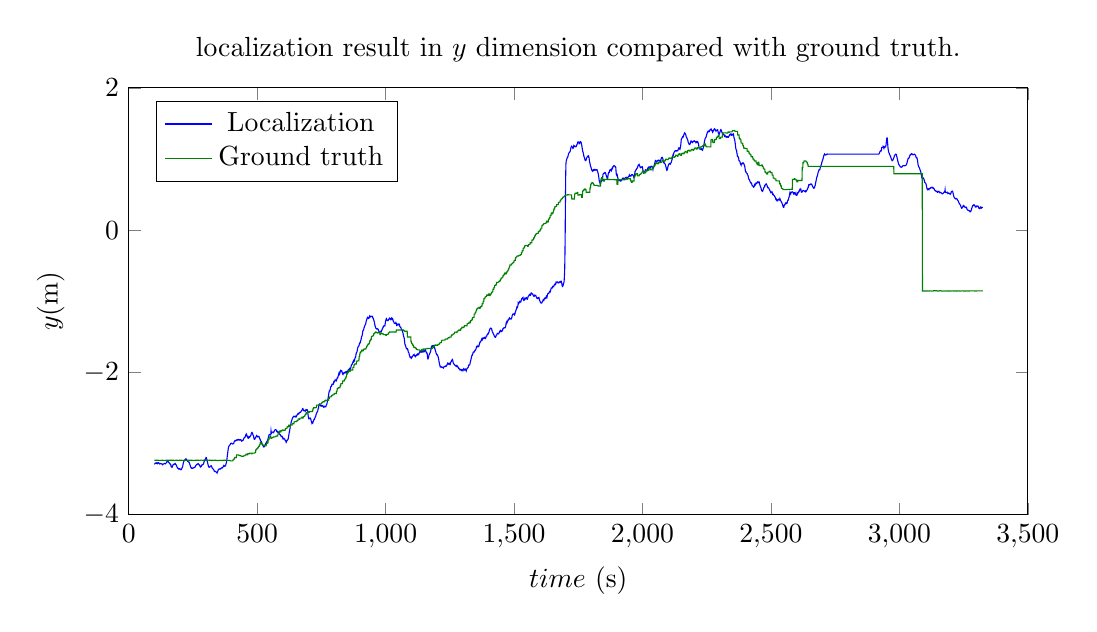
\begin{tikzpicture}

\begin{axis}[
title={localization result in $y$ dimension compared with ground truth.},
xlabel={$time$ (s)},
ylabel={$y$(m)},
xmin=0, xmax=3500,
ymin=-4, ymax=2,
axis on top,
width=13cm,
height=7cm,
legend style={at={(0.03,0.97)}, anchor=north west},
legend entries={{Localization},{Ground truth}}
]
\addplot [blue]
coordinates {
(100,-3.2860701084137)
(101,-3.28796315193176)
(102,-3.28367424011231)
(103,-3.27935099601746)
(104,-3.2794816493988)
(105,-3.2782199382782)
(106,-3.27519917488098)
(107,-3.27994608879089)
(108,-3.27937960624695)
(109,-3.27606081962585)
(110,-3.28106093406677)
(111,-3.28556799888611)
(112,-3.28121662139893)
(113,-3.28059053421021)
(114,-3.27076411247253)
(115,-3.27081727981567)
(116,-3.27228450775147)
(117,-3.27255368232727)
(118,-3.27720451354981)
(119,-3.28560423851013)
(120,-3.28918600082398)
(121,-3.29047274589539)
(122,-3.28445363044739)
(123,-3.2837438583374)
(124,-3.28250193595886)
(125,-3.28311085700989)
(126,-3.28348875045776)
(127,-3.28608727455139)
(128,-3.28718113899231)
(129,-3.28730416297913)
(130,-3.29078078269959)
(131,-3.29502058029175)
(132,-3.29947400093079)
(133,-3.29361343383789)
(134,-3.29209589958191)
(135,-3.29214668273926)
(136,-3.28830885887146)
(137,-3.28479075431824)
(138,-3.28362679481506)
(139,-3.28091049194336)
(140,-3.28279423713684)
(141,-3.28437519073486)
(142,-3.28784251213074)
(143,-3.28655529022217)
(144,-3.28159213066101)
(145,-3.27747082710266)
(146,-3.27314448356628)
(147,-3.26968288421631)
(148,-3.26238679885864)
(149,-3.25385665893555)
(150,-3.25691795349121)
(151,-3.25683569908142)
(152,-3.25230288505554)
(153,-3.25460600852966)
(154,-3.25812387466431)
(155,-3.263911485672)
(156,-3.26526737213135)
(157,-3.27016496658325)
(158,-3.27521204948425)
(159,-3.28393006324768)
(160,-3.28725481033325)
(161,-3.28724646568298)
(162,-3.29032754898071)
(163,-3.29044079780579)
(164,-3.30611419677734)
(165,-3.32526922225952)
(166,-3.32955837249756)
(167,-3.32563591003418)
(168,-3.32298254966736)
(169,-3.33247566223145)
(170,-3.32587790489197)
(171,-3.31854820251465)
(172,-3.3050479888916)
(173,-3.30168986320496)
(174,-3.29637789726257)
(175,-3.29330563545227)
(176,-3.29379940032959)
(177,-3.29117965698242)
(178,-3.29239058494568)
(179,-3.29058504104614)
(180,-3.28531980514526)
(181,-3.28196907043457)
(182,-3.28831958770752)
(183,-3.29689693450928)
(184,-3.29888510704041)
(185,-3.30528926849365)
(186,-3.30990743637085)
(187,-3.32011675834656)
(188,-3.33060550689697)
(189,-3.33828926086426)
(190,-3.34776711463928)
(191,-3.34870386123657)
(192,-3.3487548828125)
(193,-3.35282492637634)
(194,-3.35800361633301)
(195,-3.35371780395508)
(196,-3.35506105422974)
(197,-3.35810947418213)
(198,-3.35486221313477)
(199,-3.35420870780945)
(200,-3.36574792861939)
(201,-3.36600303649902)
(202,-3.36951684951782)
(203,-3.37049746513367)
(204,-3.36879205703735)
(205,-3.36492800712585)
(206,-3.36036896705627)
(207,-3.34622168540955)
(208,-3.33838081359863)
(209,-3.33227205276489)
(210,-3.32539248466492)
(211,-3.30945253372192)
(212,-3.28434610366821)
(213,-3.26965427398682)
(214,-3.25827717781067)
(215,-3.25117087364197)
(216,-3.24421262741089)
(217,-3.23873090744019)
(218,-3.2323477268219)
(219,-3.23362755775452)
(220,-3.23278021812439)
(221,-3.21950674057007)
(222,-3.21700286865234)
(223,-3.21595215797424)
(224,-3.22203421592712)
(225,-3.22823143005371)
(226,-3.22984647750855)
(227,-3.23763036727905)
(228,-3.24344038963318)
(229,-3.24718713760376)
(230,-3.25164246559143)
(231,-3.25651121139526)
(232,-3.26056027412415)
(233,-3.25931167602539)
(234,-3.25904440879822)
(235,-3.26605653762817)
(236,-3.27229952812195)
(237,-3.28434181213379)
(238,-3.29384779930115)
(239,-3.30666875839233)
(240,-3.31837940216064)
(241,-3.32989120483398)
(242,-3.33822202682495)
(243,-3.34031581878662)
(244,-3.34810566902161)
(245,-3.35017967224121)
(246,-3.34754109382629)
(247,-3.34596800804138)
(248,-3.34923005104065)
(249,-3.34789967536926)
(250,-3.34957456588745)
(251,-3.34569430351257)
(252,-3.34407925605774)
(253,-3.34221434593201)
(254,-3.33962774276733)
(255,-3.33614993095398)
(256,-3.33566498756409)
(257,-3.33736944198608)
(258,-3.33381152153015)
(259,-3.32863712310791)
(260,-3.31938624382019)
(261,-3.31279492378235)
(262,-3.30990171432495)
(263,-3.30272316932678)
(264,-3.29691910743713)
(265,-3.29817533493042)
(266,-3.29724454879761)
(267,-3.29401445388794)
(268,-3.29204869270325)
(269,-3.28578639030457)
(270,-3.2822904586792)
(271,-3.28437376022339)
(272,-3.29071593284607)
(273,-3.29666781425476)
(274,-3.30273246765137)
(275,-3.30249285697937)
(276,-3.31157565116882)
(277,-3.31862378120422)
(278,-3.32333421707153)
(279,-3.32889986038208)
(280,-3.32149577140808)
(281,-3.32463073730469)
(282,-3.32535457611084)
(283,-3.3206033706665)
(284,-3.31107068061829)
(285,-3.30171203613281)
(286,-3.29774832725525)
(287,-3.29733538627625)
(288,-3.29865479469299)
(289,-3.29459953308106)
(290,-3.29335594177246)
(291,-3.28773951530457)
(292,-3.27700328826904)
(293,-3.26249957084656)
(294,-3.25444054603577)
(295,-3.24658060073853)
(296,-3.23383808135986)
(297,-3.22849917411804)
(298,-3.22409224510193)
(299,-3.21548175811768)
(300,-3.21157383918762)
(301,-3.19935584068298)
(302,-3.20033860206604)
(303,-3.21342349052429)
(304,-3.22488307952881)
(305,-3.23915886878967)
(306,-3.25521874427795)
(307,-3.27070069313049)
(308,-3.28678965568543)
(309,-3.3009819984436)
(310,-3.31705045700073)
(311,-3.32777428627014)
(312,-3.33403825759888)
(313,-3.33530306816101)
(314,-3.33527612686157)
(315,-3.33441710472107)
(316,-3.33188915252686)
(317,-3.32411742210388)
(318,-3.31967854499817)
(319,-3.31800007820129)
(320,-3.31667613983154)
(321,-3.31428742408752)
(322,-3.31642866134644)
(323,-3.32463812828064)
(324,-3.33449029922485)
(325,-3.34801912307739)
(326,-3.35010409355164)
(327,-3.3527626991272)
(328,-3.35727763175964)
(329,-3.3621301651001)
(330,-3.36520671844482)
(331,-3.37100028991699)
(332,-3.37890577316284)
(333,-3.38842797279358)
(334,-3.39058947563171)
(335,-3.3948540687561)
(336,-3.39490532875061)
(337,-3.39262223243713)
(338,-3.39317774772644)
(339,-3.39608860015869)
(340,-3.40044975280762)
(341,-3.40325212478638)
(342,-3.40511965751648)
(343,-3.41205549240112)
(344,-3.41767477989197)
(345,-3.40358686447144)
(346,-3.40043926239014)
(347,-3.38894701004028)
(348,-3.37821936607361)
(349,-3.36905765533447)
(350,-3.36441230773926)
(351,-3.36246800422669)
(352,-3.36016941070557)
(353,-3.36257791519165)
(354,-3.36181879043579)
(355,-3.35733485221863)
(356,-3.35648226737976)
(357,-3.35605025291443)
(358,-3.35907220840454)
(359,-3.35513353347778)
(360,-3.34687852859497)
(361,-3.34470462799072)
(362,-3.34300804138184)
(363,-3.34441542625427)
(364,-3.34104418754578)
(365,-3.34389495849609)
(366,-3.33819031715393)
(367,-3.33496046066284)
(368,-3.32634687423706)
(369,-3.31920409202576)
(370,-3.31140804290772)
(371,-3.3163480758667)
(372,-3.31486105918884)
(373,-3.31926107406616)
(374,-3.32195138931274)
(375,-3.31923484802246)
(376,-3.31726264953613)
(377,-3.31188654899597)
(378,-3.29833745956421)
(379,-3.28572249412537)
(380,-3.27370166778564)
(381,-3.25382518768311)
(382,-3.23468828201294)
(383,-3.20175933837891)
(384,-3.1689715385437)
(385,-3.14606308937073)
(386,-3.11552453041077)
(387,-3.08422946929932)
(388,-3.06283783912659)
(389,-3.04807281494141)
(390,-3.04242753982544)
(391,-3.03465080261231)
(392,-3.02978801727295)
(393,-3.02520418167114)
(394,-3.02083969116211)
(395,-3.01602005958557)
(396,-3.012131690979)
(397,-3.00073885917664)
(398,-2.99904537200928)
(399,-2.99696636199951)
(400,-3.00016450881958)
(401,-3.00086951255798)
(402,-3.00112104415894)
(403,-3.00173330307007)
(404,-3.0077531337738)
(405,-3.00694918632507)
(406,-3.00666379928589)
(407,-3.00685358047485)
(408,-3.00434899330139)
(409,-2.997478723526)
(410,-2.98160529136658)
(411,-2.97436189651489)
(412,-2.96969199180603)
(413,-2.96386241912842)
(414,-2.96763515472412)
(415,-2.96563744544983)
(416,-2.96042084693909)
(417,-2.95682787895203)
(418,-2.95561623573303)
(419,-2.95676708221436)
(420,-2.95340204238892)
(421,-2.95718097686768)
(422,-2.94752287864685)
(423,-2.94657778739929)
(424,-2.94742965698242)
(425,-2.94600105285645)
(426,-2.95083856582642)
(427,-2.9477276802063)
(428,-2.94433307647705)
(429,-2.94727301597595)
(430,-2.9529914855957)
(431,-2.954021692276)
(432,-2.94875478744507)
(433,-2.95081329345703)
(434,-2.95260810852051)
(435,-2.94775724411011)
(436,-2.94804906845093)
(437,-2.94877767562866)
(438,-2.95395350456238)
(439,-2.96621584892273)
(440,-2.96918439865112)
(441,-2.96878266334534)
(442,-2.95939254760742)
(443,-2.95850419998169)
(444,-2.95800566673279)
(445,-2.95781064033508)
(446,-2.94835519790649)
(447,-2.9388599395752)
(448,-2.93308043479919)
(449,-2.92577886581421)
(450,-2.92023420333862)
(451,-2.91606712341309)
(452,-2.91270565986633)
(453,-2.91068196296692)
(454,-2.90551567077637)
(455,-2.88714218139648)
(456,-2.8790488243103)
(457,-2.88857769966126)
(458,-2.88343214988709)
(459,-2.87441563606262)
(460,-2.89325141906738)
(461,-2.89438199996948)
(462,-2.9037036895752)
(463,-2.90984797477722)
(464,-2.92149305343628)
(465,-2.92829394340515)
(466,-2.92623805999756)
(467,-2.91564393043518)
(468,-2.903639793396)
(469,-2.9057993888855)
(470,-2.91599035263062)
(471,-2.91217803955078)
(472,-2.90759563446045)
(473,-2.89889597892761)
(474,-2.89323449134827)
(475,-2.88878011703491)
(476,-2.88279485702515)
(477,-2.86691093444824)
(478,-2.85285687446594)
(479,-2.84647226333618)
(480,-2.84513378143311)
(481,-2.85120868682861)
(482,-2.86154627799988)
(483,-2.86888837814331)
(484,-2.88089966773987)
(485,-2.88773608207703)
(486,-2.90122532844544)
(487,-2.91848349571228)
(488,-2.93198561668396)
(489,-2.94278168678284)
(490,-2.94410395622253)
(491,-2.93599128723145)
(492,-2.93016076087952)
(493,-2.92354393005371)
(494,-2.91499280929565)
(495,-2.911696434021)
(496,-2.90178060531616)
(497,-2.89661359786987)
(498,-2.88918018341064)
(499,-2.89391469955444)
(500,-2.89686131477356)
(501,-2.9028000831604)
(502,-2.90755081176758)
(503,-2.905916929245)
(504,-2.90367031097412)
(505,-2.90269708633423)
(506,-2.90584707260132)
(507,-2.90387630462647)
(508,-2.90969729423523)
(509,-2.92243599891663)
(510,-2.9344527721405)
(511,-2.93686938285828)
(512,-2.94520211219788)
(513,-2.9599130153656)
(514,-2.96803855895996)
(515,-2.96877956390381)
(516,-2.97051382064819)
(517,-2.97924566268921)
(518,-2.9916980266571)
(519,-3.00501227378845)
(520,-3.01576852798462)
(521,-3.02075386047363)
(522,-3.02728796005249)
(523,-3.02939629554749)
(524,-3.04530239105225)
(525,-3.04946827888489)
(526,-3.05008363723755)
(527,-3.04906964302063)
(528,-3.04610633850098)
(529,-3.03478789329529)
(530,-3.03109288215637)
(531,-3.02345705032349)
(532,-3.0124135017395)
(533,-3.00221538543701)
(534,-2.99646353721619)
(535,-2.99035501480103)
(536,-2.98349857330322)
(537,-2.97850370407105)
(538,-2.98045063018799)
(539,-2.97283244132996)
(540,-2.95933198928833)
(541,-2.95287680625916)
(542,-2.9379870891571)
(543,-2.92577815055847)
(544,-2.91213011741638)
(545,-2.89432406425476)
(546,-2.88263750076294)
(547,-2.87846755981445)
(548,-2.8722939491272)
(549,-2.87232637405396)
(550,-2.87922596931458)
(551,-2.88165593147278)
(552,-2.87909007072449)
(553,-2.87112498283386)
(554,-2.82432007789612)
(555,-2.85322070121765)
(556,-2.85572671890259)
(557,-2.8457088470459)
(558,-2.84339380264282)
(559,-2.84106516838074)
(560,-2.84040260314941)
(561,-2.83996844291687)
(562,-2.83967447280884)
(563,-2.84872341156006)
(564,-2.84628582000732)
(565,-2.84004139900208)
(566,-2.8296549320221)
(567,-2.82445502281189)
(568,-2.81399917602539)
(569,-2.81203985214233)
(570,-2.80788326263428)
(571,-2.80767107009888)
(572,-2.80653715133667)
(573,-2.80987286567688)
(574,-2.81111550331116)
(575,-2.81643676757813)
(576,-2.83110117912293)
(577,-2.8355770111084)
(578,-2.83288073539734)
(579,-2.83053207397461)
(580,-2.83402943611145)
(581,-2.84669423103333)
(582,-2.84545803070068)
(583,-2.84558773040772)
(584,-2.84206819534302)
(585,-2.85009002685547)
(586,-2.85074877738953)
(587,-2.86096835136414)
(588,-2.87202405929565)
(589,-2.87682867050171)
(590,-2.87789559364319)
(591,-2.88499093055725)
(592,-2.89156532287598)
(593,-2.89695858955383)
(594,-2.90544009208679)
(595,-2.90617346763611)
(596,-2.89853811264038)
(597,-2.89834690093994)
(598,-2.90578055381775)
(599,-2.91590929031372)
(600,-2.9303503036499)
(601,-2.93896913528442)
(602,-2.93656229972839)
(603,-2.9328145980835)
(604,-2.92878127098084)
(605,-2.93403768539429)
(606,-2.93524694442749)
(607,-2.93687295913696)
(608,-2.95237231254578)
(609,-2.95286679267883)
(610,-2.95568871498108)
(611,-2.96451282501221)
(612,-2.97011756896973)
(613,-2.98410177230835)
(614,-2.97613954544067)
(615,-2.96369814872742)
(616,-2.96113109588623)
(617,-2.95481443405151)
(618,-2.95420169830322)
(619,-2.94833636283875)
(620,-2.94085788726807)
(621,-2.93629288673401)
(622,-2.91272306442261)
(623,-2.88743352890015)
(624,-2.86565065383911)
(625,-2.84787535667419)
(626,-2.83211255073547)
(627,-2.8087739944458)
(628,-2.78744673728943)
(629,-2.7612841129303)
(630,-2.75148296356201)
(631,-2.73173069953919)
(632,-2.70913863182068)
(633,-2.6947009563446)
(634,-2.68126344680786)
(635,-2.67171764373779)
(636,-2.66001534461975)
(637,-2.65456366539002)
(638,-2.6411349773407)
(639,-2.63625526428223)
(640,-2.62808108329773)
(641,-2.62597703933716)
(642,-2.62041687965393)
(643,-2.62331080436707)
(644,-2.62598013877869)
(645,-2.62444448471069)
(646,-2.62212324142456)
(647,-2.61816835403442)
(648,-2.61547517776489)
(649,-2.62461686134338)
(650,-2.62855863571167)
(651,-2.62920618057251)
(652,-2.62705326080322)
(653,-2.62163972854614)
(654,-2.61187291145325)
(655,-2.60374331474304)
(656,-2.59496569633484)
(657,-2.59368252754211)
(658,-2.58417105674744)
(659,-2.5811607837677)
(660,-2.57778882980347)
(661,-2.5758273601532)
(662,-2.58305239677429)
(663,-2.5750002861023)
(664,-2.57411098480225)
(665,-2.56549668312073)
(666,-2.56272387504578)
(667,-2.56446385383606)
(668,-2.56438946723938)
(669,-2.55996751785278)
(670,-2.55636429786682)
(671,-2.54985046386719)
(672,-2.543781042099)
(673,-2.53768563270569)
(674,-2.53685545921326)
(675,-2.53020453453064)
(676,-2.52193164825439)
(677,-2.50977945327759)
(678,-2.51142692565918)
(679,-2.52046298980713)
(680,-2.52946639060974)
(681,-2.53844523429871)
(682,-2.54045295715332)
(683,-2.53657126426697)
(684,-2.5357551574707)
(685,-2.53596472740173)
(686,-2.53790926933289)
(687,-2.54710268974304)
(688,-2.53727722167969)
(689,-2.53502774238586)
(690,-2.52658486366272)
(691,-2.53159546852112)
(692,-2.5343976020813)
(693,-2.52974939346314)
(694,-2.52623462677002)
(695,-2.52867674827576)
(696,-2.53822588920593)
(697,-2.56701612472534)
(698,-2.59091806411743)
(699,-2.61849641799927)
(700,-2.63758707046509)
(701,-2.65157866477966)
(702,-2.6479663848877)
(703,-2.64723324775696)
(704,-2.65074706077576)
(705,-2.64751410484314)
(706,-2.64398813247681)
(707,-2.64346313476563)
(708,-2.65126490592957)
(709,-2.66045308113098)
(710,-2.67833662033081)
(711,-2.6926896572113)
(712,-2.69915270805359)
(713,-2.71290302276611)
(714,-2.70329308509827)
(715,-2.69982266426086)
(716,-2.69747352600098)
(717,-2.70710682868958)
(718,-2.69556140899658)
(719,-2.68375492095947)
(720,-2.67101812362671)
(721,-2.66574931144714)
(722,-2.66102933883667)
(723,-2.66224217414856)
(724,-2.65188694000244)
(725,-2.64056825637817)
(726,-2.62793254852295)
(727,-2.62560677528381)
(728,-2.61708378791809)
(729,-2.59901332855225)
(730,-2.58699202537537)
(731,-2.57615947723389)
(732,-2.56990742683411)
(733,-2.56379294395447)
(734,-2.55659699440002)
(735,-2.55041003227234)
(736,-2.53989720344544)
(737,-2.52001786231995)
(738,-2.50648736953735)
(739,-2.50450539588928)
(740,-2.46839690208435)
(741,-2.46012020111084)
(742,-2.45219492912293)
(743,-2.45417737960815)
(744,-2.44726991653442)
(745,-2.45308780670166)
(746,-2.466064453125)
(747,-2.47148370742798)
(748,-2.47385168075562)
(749,-2.46907377243042)
(750,-2.4673318862915)
(751,-2.46758437156677)
(752,-2.47516775131226)
(753,-2.47323727607727)
(754,-2.46774315834045)
(755,-2.46656608581543)
(756,-2.47380995750427)
(757,-2.48193359375)
(758,-2.4890148639679)
(759,-2.4916512966156)
(760,-2.49272346496582)
(761,-2.48187303543091)
(762,-2.47805595397949)
(763,-2.47854828834534)
(764,-2.48353457450867)
(765,-2.48395013809204)
(766,-2.48465895652771)
(767,-2.48563742637634)
(768,-2.47653746604919)
(769,-2.46150207519531)
(770,-2.45911645889282)
(771,-2.4515974521637)
(772,-2.43500328063965)
(773,-2.41384196281433)
(774,-2.39467215538025)
(775,-2.38495421409607)
(776,-2.36850547790527)
(777,-2.3450825214386)
(778,-2.3233654499054)
(779,-2.29963803291321)
(780,-2.27767610549927)
(781,-2.26066398620606)
(782,-2.25679206848145)
(783,-2.25928330421448)
(784,-2.24715375900269)
(785,-2.23359370231628)
(786,-2.21276831626892)
(787,-2.19973134994507)
(788,-2.19556427001953)
(789,-2.19572877883911)
(790,-2.18507814407349)
(791,-2.17343688011169)
(792,-2.16688919067383)
(793,-2.16938376426697)
(794,-2.16724872589111)
(795,-2.1707706451416)
(796,-2.16993355751038)
(797,-2.16040515899658)
(798,-2.13729691505432)
(799,-2.12784075737)
(800,-2.12892317771912)
(801,-2.13197827339172)
(802,-2.11918210983276)
(803,-2.11704444885254)
(804,-2.10700392723084)
(805,-2.11262106895447)
(806,-2.11035060882568)
(807,-2.11044239997864)
(808,-2.11925530433655)
(809,-2.11389589309692)
(810,-2.09949350357056)
(811,-2.08567190170288)
(812,-2.07562923431397)
(813,-2.07690501213074)
(814,-2.07660484313965)
(815,-2.06064224243164)
(816,-2.04602789878845)
(817,-2.03003025054932)
(818,-2.01803803443909)
(819,-2.00582098960877)
(820,-2.01291990280151)
(821,-2.02432727813721)
(822,-2.01454925537109)
(823,-1.99893093109131)
(824,-1.97931671142578)
(825,-1.97403347492218)
(826,-1.98240983486176)
(827,-1.97869563102722)
(828,-1.97536039352417)
(829,-1.97607386112213)
(830,-1.98847913742065)
(831,-2.00300288200378)
(832,-2.01059007644653)
(833,-2.02627754211426)
(834,-2.03105521202087)
(835,-2.02045893669128)
(836,-2.01311612129211)
(837,-2.00949025154114)
(838,-2.01455092430115)
(839,-2.01236462593079)
(840,-2.00748348236084)
(841,-2.0011568069458)
(842,-1.9974182844162)
(843,-1.99450600147247)
(844,-2.00007605552673)
(845,-2.00652241706848)
(846,-2.0021116733551)
(847,-1.99779617786408)
(848,-1.99083590507507)
(849,-1.9887707233429)
(850,-1.98665964603424)
(851,-1.99797141551972)
(852,-1.99403691291809)
(853,-1.98667824268341)
(854,-1.97286558151245)
(855,-1.96373128890991)
(856,-1.96149396896362)
(857,-1.96603572368622)
(858,-1.97235465049744)
(859,-1.96001327037811)
(860,-1.94685781002045)
(861,-1.94069039821625)
(862,-1.94105315208435)
(863,-1.95115494728088)
(864,-1.94452893733978)
(865,-1.92690193653107)
(866,-1.91057586669922)
(867,-1.89774084091187)
(868,-1.89175808429718)
(869,-1.88833582401276)
(870,-1.88595354557037)
(871,-1.87300205230713)
(872,-1.86567890644074)
(873,-1.85515749454498)
(874,-1.84733986854553)
(875,-1.83848476409912)
(876,-1.85392701625824)
(877,-1.85094213485718)
(878,-1.84183037281036)
(879,-1.83507490158081)
(880,-1.81267988681793)
(881,-1.80419790744782)
(882,-1.78799521923065)
(883,-1.78801441192627)
(884,-1.77100706100464)
(885,-1.74117493629456)
(886,-1.72917795181274)
(887,-1.72208869457245)
(888,-1.71763622760773)
(889,-1.70778048038483)
(890,-1.68606543540955)
(891,-1.66533172130585)
(892,-1.65012717247009)
(893,-1.64171981811524)
(894,-1.63465893268585)
(895,-1.633584856987)
(896,-1.63138544559479)
(897,-1.6152857542038)
(898,-1.59660959243774)
(899,-1.58777356147766)
(900,-1.58550262451172)
(901,-1.58654057979584)
(902,-1.57118725776672)
(903,-1.55811655521393)
(904,-1.54768717288971)
(905,-1.52859020233154)
(906,-1.50713920593262)
(907,-1.49447929859161)
(908,-1.48841381072998)
(909,-1.47820556163788)
(910,-1.45589637756348)
(911,-1.42907607555389)
(912,-1.41255271434784)
(913,-1.40966606140137)
(914,-1.40780711174011)
(915,-1.39320635795593)
(916,-1.37360012531281)
(917,-1.36589467525482)
(918,-1.35585057735443)
(919,-1.34531152248383)
(920,-1.33486533164978)
(921,-1.33361923694611)
(922,-1.32746064662933)
(923,-1.3106826543808)
(924,-1.29169130325317)
(925,-1.27543377876282)
(926,-1.26623451709747)
(927,-1.25771427154541)
(928,-1.24062836170197)
(929,-1.2310916185379)
(930,-1.22596514225006)
(931,-1.22944569587708)
(932,-1.23387730121613)
(933,-1.2381466627121)
(934,-1.24326252937317)
(935,-1.24208176136017)
(936,-1.23434507846832)
(937,-1.21767318248749)
(938,-1.20990717411041)
(939,-1.22227799892426)
(940,-1.22379684448242)
(941,-1.22092509269714)
(942,-1.21717500686646)
(943,-1.21117544174194)
(944,-1.21013200283051)
(945,-1.211953997612)
(946,-1.21275758743286)
(947,-1.2156982421875)
(948,-1.21950054168701)
(949,-1.21696698665619)
(950,-1.23472464084625)
(951,-1.23651075363159)
(952,-1.24024200439453)
(953,-1.25301933288574)
(954,-1.26336920261383)
(955,-1.2780601978302)
(956,-1.29043519496918)
(957,-1.30801093578339)
(958,-1.32818353176117)
(959,-1.34570920467377)
(960,-1.3593020439148)
(961,-1.3676038980484)
(962,-1.37847626209259)
(963,-1.38375401496887)
(964,-1.38664269447327)
(965,-1.38632535934448)
(966,-1.39181935787201)
(967,-1.39255917072296)
(968,-1.39097690582275)
(969,-1.38704705238342)
(970,-1.39247894287109)
(971,-1.39707112312317)
(972,-1.40579175949097)
(973,-1.4142062664032)
(974,-1.42676520347595)
(975,-1.43575823307037)
(976,-1.43873274326325)
(977,-1.43320393562317)
(978,-1.43582105636597)
(979,-1.43506932258606)
(980,-1.43170297145844)
(981,-1.42807602882385)
(982,-1.4255542755127)
(983,-1.41817688941956)
(984,-1.42056941986084)
(985,-1.4129364490509)
(986,-1.40050983428955)
(987,-1.39179408550263)
(988,-1.38064992427826)
(989,-1.37593472003937)
(990,-1.3740017414093)
(991,-1.35546553134918)
(992,-1.35670876502991)
(993,-1.34668731689453)
(994,-1.34522676467896)
(995,-1.34560751914978)
(996,-1.34574997425079)
(997,-1.34692227840424)
(998,-1.32772564888001)
(999,-1.30198657512665)
(1000,-1.28125107288361)
(1001,-1.26685166358948)
(1002,-1.25356066226959)
(1003,-1.24579608440399)
(1004,-1.25372648239136)
(1005,-1.26469600200653)
(1006,-1.26665329933167)
(1007,-1.27005648612976)
(1008,-1.27266478538513)
(1009,-1.27491879463196)
(1010,-1.26930236816406)
(1011,-1.26140427589417)
(1012,-1.25512039661408)
(1013,-1.25391471385956)
(1014,-1.2484267950058)
(1015,-1.23612332344055)
(1016,-1.23710751533508)
(1017,-1.24319171905518)
(1018,-1.25097191333771)
(1019,-1.24488759040833)
(1020,-1.24645495414734)
(1021,-1.25643360614777)
(1022,-1.25096547603607)
(1023,-1.24813747406006)
(1024,-1.23510360717774)
(1025,-1.2388641834259)
(1026,-1.25228679180145)
(1027,-1.24729216098785)
(1028,-1.25282180309296)
(1029,-1.26323294639587)
(1030,-1.2821501493454)
(1031,-1.28888821601868)
(1032,-1.29304230213165)
(1033,-1.30019998550415)
(1034,-1.31114172935486)
(1035,-1.31120479106903)
(1036,-1.31305837631226)
(1037,-1.31243276596069)
(1038,-1.31350469589233)
(1039,-1.30701792240143)
(1040,-1.30047476291657)
(1041,-1.31047427654266)
(1042,-1.31666779518128)
(1043,-1.33565974235535)
(1044,-1.32945418357849)
(1045,-1.32319676876068)
(1046,-1.33018338680267)
(1047,-1.3334858417511)
(1048,-1.33664691448212)
(1049,-1.33054351806641)
(1050,-1.32717788219452)
(1051,-1.32775890827179)
(1052,-1.31999361515045)
(1053,-1.32392144203186)
(1054,-1.33023405075073)
(1055,-1.34879326820374)
(1056,-1.35875082015991)
(1057,-1.36067295074463)
(1058,-1.36836993694305)
(1059,-1.36828577518463)
(1060,-1.37613487243652)
(1061,-1.3897876739502)
(1062,-1.3997768163681)
(1063,-1.40603244304657)
(1064,-1.41127622127533)
(1065,-1.41016614437103)
(1066,-1.42460882663727)
(1067,-1.44314920902252)
(1068,-1.45327925682068)
(1069,-1.47481441497803)
(1070,-1.49318599700928)
(1071,-1.50256025791168)
(1072,-1.512455701828)
(1073,-1.53304243087769)
(1074,-1.57391202449799)
(1075,-1.59982240200043)
(1076,-1.61499202251434)
(1077,-1.61697089672089)
(1078,-1.62287855148315)
(1079,-1.64474523067474)
(1080,-1.65561139583588)
(1081,-1.66417455673218)
(1082,-1.66880023479462)
(1083,-1.67063999176025)
(1084,-1.66852414608002)
(1085,-1.66772961616516)
(1086,-1.67566883563995)
(1087,-1.69034349918366)
(1088,-1.70915508270264)
(1089,-1.71968686580658)
(1090,-1.72243690490723)
(1091,-1.72879159450531)
(1092,-1.74767231941223)
(1093,-1.76450765132904)
(1094,-1.77174735069275)
(1095,-1.78697645664215)
(1096,-1.79217720031738)
(1097,-1.78557538986206)
(1098,-1.78548753261566)
(1099,-1.78905999660492)
(1100,-1.79529905319214)
(1101,-1.8007082939148)
(1102,-1.79110932350159)
(1103,-1.78254318237305)
(1104,-1.78324091434479)
(1105,-1.77817690372467)
(1106,-1.76995599269867)
(1107,-1.76095926761627)
(1108,-1.75769019126892)
(1109,-1.75895738601685)
(1110,-1.75253129005432)
(1111,-1.74872016906738)
(1112,-1.75936102867127)
(1113,-1.77032065391541)
(1114,-1.77118313312531)
(1115,-1.76709091663361)
(1116,-1.76959669589996)
(1117,-1.77752196788788)
(1118,-1.76997578144074)
(1119,-1.76062977313995)
(1120,-1.75417292118073)
(1121,-1.75283241271973)
(1122,-1.75654530525208)
(1123,-1.75020349025726)
(1124,-1.74088191986084)
(1125,-1.74191009998322)
(1126,-1.75209379196167)
(1127,-1.7496964931488)
(1128,-1.74306535720825)
(1129,-1.74752771854401)
(1130,-1.73812079429627)
(1131,-1.72772836685181)
(1132,-1.7185789346695)
(1133,-1.71078038215637)
(1134,-1.70939326286316)
(1135,-1.71373879909515)
(1136,-1.70903253555298)
(1137,-1.71007978916168)
(1138,-1.70983517169952)
(1139,-1.71679353713989)
(1140,-1.71764552593231)
(1141,-1.71578776836395)
(1142,-1.70936000347138)
(1143,-1.69718158245087)
(1144,-1.701580286026)
(1145,-1.70914328098297)
(1146,-1.70496988296509)
(1147,-1.70964694023132)
(1148,-1.70123553276062)
(1149,-1.70723354816437)
(1150,-1.71052849292755)
(1151,-1.70948576927185)
(1152,-1.70056045055389)
(1153,-1.68823146820068)
(1154,-1.68313276767731)
(1155,-1.68275237083435)
(1156,-1.69499671459198)
(1157,-1.70222246646881)
(1158,-1.71584630012512)
(1159,-1.72675061225891)
(1160,-1.72585320472717)
(1161,-1.72586977481842)
(1162,-1.73958778381348)
(1163,-1.77080321311951)
(1164,-1.80281460285187)
(1165,-1.81118524074555)
(1166,-1.80533051490784)
(1167,-1.78792440891266)
(1168,-1.77263402938843)
(1169,-1.75670802593231)
(1170,-1.74973475933075)
(1171,-1.74415385723114)
(1172,-1.73634517192841)
(1173,-1.72353565692902)
(1174,-1.71709001064301)
(1175,-1.70794856548309)
(1176,-1.69414186477661)
(1177,-1.67537534236908)
(1178,-1.6591203212738)
(1179,-1.63877630233765)
(1180,-1.6339772939682)
(1181,-1.62684464454651)
(1182,-1.62551319599152)
(1183,-1.62892532348633)
(1184,-1.63438105583191)
(1185,-1.62723290920258)
(1186,-1.62534248828888)
(1187,-1.63611900806427)
(1188,-1.63951742649078)
(1189,-1.64557147026062)
(1190,-1.64517557621002)
(1191,-1.65649664402008)
(1192,-1.67059206962586)
(1193,-1.68203568458557)
(1194,-1.69547522068024)
(1195,-1.70403492450714)
(1196,-1.72318708896637)
(1197,-1.73355829715729)
(1198,-1.74044024944305)
(1199,-1.75216686725617)
(1200,-1.75417232513428)
(1201,-1.75381946563721)
(1202,-1.75886142253876)
(1203,-1.76826274394989)
(1204,-1.77694940567017)
(1205,-1.7905809879303)
(1206,-1.80466175079346)
(1207,-1.82567667961121)
(1208,-1.84951961040497)
(1209,-1.86516308784485)
(1210,-1.88861906528473)
(1211,-1.89766049385071)
(1212,-1.91421103477478)
(1213,-1.92612588405609)
(1214,-1.92607843875885)
(1215,-1.91872799396515)
(1216,-1.91861236095429)
(1217,-1.92609369754791)
(1218,-1.92736184597015)
(1219,-1.9325190782547)
(1220,-1.93159317970276)
(1221,-1.93178188800812)
(1222,-1.93296456336975)
(1223,-1.92953360080719)
(1224,-1.93449115753174)
(1225,-1.93916690349579)
(1226,-1.93166434764862)
(1227,-1.92699790000916)
(1228,-1.92120599746704)
(1229,-1.91773080825806)
(1230,-1.9179550409317)
(1231,-1.91887080669403)
(1232,-1.91518771648407)
(1233,-1.91302824020386)
(1234,-1.91498959064484)
(1235,-1.9128954410553)
(1236,-1.90738785266876)
(1237,-1.91036653518677)
(1238,-1.90473532676697)
(1239,-1.89472627639771)
(1240,-1.88632297515869)
(1241,-1.88098561763763)
(1242,-1.87203514575958)
(1243,-1.87761902809143)
(1244,-1.88323414325714)
(1245,-1.87635219097138)
(1246,-1.87484920024872)
(1247,-1.87873589992523)
(1248,-1.8749817609787)
(1249,-1.88033545017242)
(1250,-1.89252710342407)
(1251,-1.89326751232147)
(1252,-1.87964773178101)
(1253,-1.86890327930451)
(1254,-1.8574298620224)
(1255,-1.84909510612488)
(1256,-1.84695661067963)
(1257,-1.83621895313263)
(1258,-1.82703924179077)
(1259,-1.82450664043427)
(1260,-1.81924498081207)
(1261,-1.82470643520355)
(1262,-1.84671092033386)
(1263,-1.86369383335114)
(1264,-1.87126362323761)
(1265,-1.87481558322907)
(1266,-1.88250160217285)
(1267,-1.89198923110962)
(1268,-1.89171457290649)
(1269,-1.89727962017059)
(1270,-1.90050673484802)
(1271,-1.90197992324829)
(1272,-1.90682303905487)
(1273,-1.90529358386993)
(1274,-1.91252255439758)
(1275,-1.91817092895508)
(1276,-1.91767477989197)
(1277,-1.91819763183594)
(1278,-1.90701401233673)
(1279,-1.91026604175568)
(1280,-1.91444051265717)
(1281,-1.92210245132446)
(1282,-1.93139266967774)
(1283,-1.93156743049622)
(1284,-1.9416720867157)
(1285,-1.94092392921448)
(1286,-1.94626045227051)
(1287,-1.95443248748779)
(1288,-1.95907175540924)
(1289,-1.96467530727387)
(1290,-1.96122050285339)
(1291,-1.96436274051666)
(1292,-1.95779311656952)
(1293,-1.95920276641846)
(1294,-1.96456897258759)
(1295,-1.97027933597565)
(1296,-1.97500860691071)
(1297,-1.97032356262207)
(1298,-1.96427512168884)
(1299,-1.96807670593262)
(1300,-1.97292709350586)
(1301,-1.97786962985992)
(1302,-1.96995937824249)
(1303,-1.9575766324997)
(1304,-1.95010161399841)
(1305,-1.95479440689087)
(1306,-1.95320844650269)
(1307,-1.95609140396118)
(1308,-1.9688218832016)
(1309,-1.96736526489258)
(1310,-1.96074593067169)
(1311,-1.95563185214996)
(1312,-1.96058988571167)
(1313,-1.96949350833893)
(1314,-1.9810061454773)
(1315,-1.97052800655365)
(1316,-1.95558333396912)
(1317,-1.94571304321289)
(1318,-1.94010472297669)
(1319,-1.93971741199493)
(1320,-1.93757700920105)
(1321,-1.93420612812042)
(1322,-1.92619490623474)
(1323,-1.89997911453247)
(1324,-1.90120315551758)
(1325,-1.90029811859131)
(1326,-1.89978694915772)
(1327,-1.89959979057312)
(1328,-1.886554479599)
(1329,-1.87081384658814)
(1330,-1.8520245552063)
(1331,-1.83739495277405)
(1332,-1.82566809654236)
(1333,-1.81279528141022)
(1334,-1.79121565818787)
(1335,-1.77380800247192)
(1336,-1.76330709457398)
(1337,-1.76302552223206)
(1338,-1.75572073459625)
(1339,-1.74612402915955)
(1340,-1.73181879520416)
(1341,-1.7171471118927)
(1342,-1.71315360069275)
(1343,-1.71386432647705)
(1344,-1.7152704000473)
(1345,-1.71547102928162)
(1346,-1.70911765098572)
(1347,-1.69939696788788)
(1348,-1.69265711307526)
(1349,-1.68667733669281)
(1350,-1.68857443332672)
(1351,-1.68092012405396)
(1352,-1.66928911209107)
(1353,-1.65637946128845)
(1354,-1.64037549495697)
(1355,-1.63405346870422)
(1356,-1.63536632061005)
(1357,-1.64075458049774)
(1358,-1.6374728679657)
(1359,-1.62929737567902)
(1360,-1.63547813892365)
(1361,-1.63855910301209)
(1362,-1.64065968990326)
(1363,-1.63802254199982)
(1364,-1.62085056304932)
(1365,-1.60427534580231)
(1366,-1.58637797832489)
(1367,-1.57765018939972)
(1368,-1.57975447177887)
(1369,-1.57375836372376)
(1370,-1.56887185573578)
(1371,-1.56292724609375)
(1372,-1.5499541759491)
(1373,-1.5497499704361)
(1374,-1.53560733795166)
(1375,-1.54302036762238)
(1376,-1.54673457145691)
(1377,-1.53832006454468)
(1378,-1.52271723747253)
(1379,-1.51669728755951)
(1380,-1.51825892925263)
(1381,-1.52348279953003)
(1382,-1.52180600166321)
(1383,-1.51626801490784)
(1384,-1.51119673252106)
(1385,-1.5090126991272)
(1386,-1.51394104957581)
(1387,-1.52075040340424)
(1388,-1.5246741771698)
(1389,-1.52071130275726)
(1390,-1.50682437419891)
(1391,-1.50604569911957)
(1392,-1.49363243579865)
(1393,-1.49123394489288)
(1394,-1.48977899551392)
(1395,-1.47868144512177)
(1396,-1.46486556529999)
(1397,-1.46122717857361)
(1398,-1.46425569057465)
(1399,-1.46017825603485)
(1400,-1.45610284805298)
(1401,-1.44675016403198)
(1402,-1.44100415706635)
(1403,-1.42713582515717)
(1404,-1.40852546691895)
(1405,-1.39584958553314)
(1406,-1.39273738861084)
(1407,-1.38998293876648)
(1408,-1.38234567642212)
(1409,-1.37825655937195)
(1410,-1.37880098819733)
(1411,-1.38278579711914)
(1412,-1.38503861427307)
(1413,-1.39027559757233)
(1414,-1.40940117835999)
(1415,-1.42462706565857)
(1416,-1.43358719348908)
(1417,-1.43651437759399)
(1418,-1.44547867774963)
(1419,-1.45967316627503)
(1420,-1.46621870994568)
(1421,-1.46682274341583)
(1422,-1.47724449634552)
(1423,-1.48766124248505)
(1424,-1.49620079994202)
(1425,-1.49578201770783)
(1426,-1.50027632713318)
(1427,-1.50836527347565)
(1428,-1.50790333747864)
(1429,-1.49773955345154)
(1430,-1.48987555503845)
(1431,-1.47975993156433)
(1432,-1.47850835323334)
(1433,-1.46986222267151)
(1434,-1.45842134952545)
(1435,-1.4536224603653)
(1436,-1.45592212677002)
(1437,-1.45541918277741)
(1438,-1.45472371578217)
(1439,-1.46005129814148)
(1440,-1.45937073230743)
(1441,-1.45483994483948)
(1442,-1.44609987735748)
(1443,-1.43872010707855)
(1444,-1.42546153068543)
(1445,-1.42619621753693)
(1446,-1.41832876205444)
(1447,-1.4085830450058)
(1448,-1.4078825712204)
(1449,-1.41563487052918)
(1450,-1.42551326751709)
(1451,-1.42090785503388)
(1452,-1.4214860200882)
(1453,-1.42191171646118)
(1454,-1.41905474662781)
(1455,-1.41537475585938)
(1456,-1.39446258544922)
(1457,-1.38537740707398)
(1458,-1.38519763946533)
(1459,-1.38482284545899)
(1460,-1.377201795578)
(1461,-1.37223994731903)
(1462,-1.37165427207947)
(1463,-1.37316262722015)
(1464,-1.37294936180115)
(1465,-1.37365305423737)
(1466,-1.36660873889923)
(1467,-1.36030507087708)
(1468,-1.34149050712586)
(1469,-1.31396472454071)
(1470,-1.30006945133209)
(1471,-1.31569743156433)
(1472,-1.3104430437088)
(1473,-1.29640173912048)
(1474,-1.29274499416351)
(1475,-1.28296482563019)
(1476,-1.26982605457306)
(1477,-1.26257908344269)
(1478,-1.26623427867889)
(1479,-1.26361572742462)
(1480,-1.25570750236511)
(1481,-1.2426096200943)
(1482,-1.23495376110077)
(1483,-1.24024736881256)
(1484,-1.24942624568939)
(1485,-1.25085699558258)
(1486,-1.24447929859161)
(1487,-1.24580585956574)
(1488,-1.24939441680908)
(1489,-1.24964439868927)
(1490,-1.24386084079742)
(1491,-1.23138117790222)
(1492,-1.22215282917023)
(1493,-1.19862806797028)
(1494,-1.18822646141052)
(1495,-1.18217992782593)
(1496,-1.18045425415039)
(1497,-1.17965638637543)
(1498,-1.18313336372376)
(1499,-1.18486571311951)
(1500,-1.18033313751221)
(1501,-1.1776978969574)
(1502,-1.19211137294769)
(1503,-1.18936860561371)
(1504,-1.16956126689911)
(1505,-1.15366625785828)
(1506,-1.14350593090057)
(1507,-1.13089501857758)
(1508,-1.12231028079987)
(1509,-1.11560010910034)
(1510,-1.09920608997345)
(1511,-1.08610677719116)
(1512,-1.09272587299347)
(1513,-1.08583092689514)
(1514,-1.07770001888275)
(1515,-1.06679511070252)
(1516,-1.03025937080383)
(1517,-1.03930056095123)
(1518,-1.03526198863983)
(1519,-1.03143000602722)
(1520,-1.0211261510849)
(1521,-1.00956404209137)
(1522,-1.00159442424774)
(1523,-1.00069057941437)
(1524,-1.00277650356293)
(1525,-1.00708830356598)
(1526,-1.01172816753388)
(1527,-1.00188910961151)
(1528,-0.988712370395661)
(1529,-0.974632263183595)
(1530,-0.963210761547089)
(1531,-0.962709903717042)
(1532,-0.958666384220124)
(1533,-0.954861104488374)
(1534,-0.959074437618256)
(1535,-0.952191174030305)
(1536,-0.972001314163209)
(1537,-0.98173749446869)
(1538,-0.988722741603852)
(1539,-0.987167358398438)
(1540,-0.981965124607087)
(1541,-0.972987115383149)
(1542,-0.956565201282502)
(1543,-0.958019018173219)
(1544,-0.967146813869477)
(1545,-0.963117122650147)
(1546,-0.960034549236298)
(1547,-0.950662314891816)
(1548,-0.94855558872223)
(1549,-0.954910874366761)
(1550,-0.961774826049805)
(1551,-0.97388118505478)
(1552,-0.971023321151734)
(1553,-0.957482814788819)
(1554,-0.947790384292603)
(1555,-0.936084747314454)
(1556,-0.9270378947258)
(1557,-0.924456715583802)
(1558,-0.92375147342682)
(1559,-0.913056433200837)
(1560,-0.904611945152283)
(1561,-0.906329333782197)
(1562,-0.911867499351502)
(1563,-0.91429477930069)
(1564,-0.916455626487733)
(1565,-0.902915298938752)
(1566,-0.891840219497681)
(1567,-0.883575320243836)
(1568,-0.884955286979676)
(1569,-0.894535958766938)
(1570,-0.892860054969788)
(1571,-0.89864331483841)
(1572,-0.899087309837342)
(1573,-0.90634971857071)
(1574,-0.910811662673951)
(1575,-0.914320170879365)
(1576,-0.922025442123414)
(1577,-0.932755768299104)
(1578,-0.933831751346589)
(1579,-0.92845380306244)
(1580,-0.918699324131013)
(1581,-0.914671659469605)
(1582,-0.921305239200593)
(1583,-0.92013829946518)
(1584,-0.921455383300782)
(1585,-0.925215482711793)
(1586,-0.932825267314912)
(1587,-0.944271743297578)
(1588,-0.950368821620942)
(1589,-0.956813573837281)
(1590,-0.964351654052735)
(1591,-0.964014232158662)
(1592,-0.959757745265961)
(1593,-0.954180419445039)
(1594,-0.958465516567231)
(1595,-0.952435910701752)
(1596,-0.946824729442597)
(1597,-0.945978939533234)
(1598,-0.965871632099152)
(1599,-0.976864993572236)
(1600,-0.992129862308503)
(1601,-0.998523890972138)
(1602,-1.00796353816986)
(1603,-1.02087843418121)
(1604,-1.02348351478577)
(1605,-1.02490746974945)
(1606,-1.02348339557648)
(1607,-1.02606976032257)
(1608,-1.02677202224732)
(1609,-1.01451897621155)
(1610,-1.00567901134491)
(1611,-1.00464928150177)
(1612,-0.996814191341401)
(1613,-0.983190178871156)
(1614,-0.978885531425477)
(1615,-0.981677532196046)
(1616,-0.986819565296174)
(1617,-0.981471121311189)
(1618,-0.965670406818391)
(1619,-0.956764698028565)
(1620,-0.954915165901185)
(1621,-0.9576855301857)
(1622,-0.962690174579621)
(1623,-0.961837649345399)
(1624,-0.951189279556275)
(1625,-0.940873742103577)
(1626,-0.931235134601594)
(1627,-0.937580466270448)
(1628,-0.946121931076051)
(1629,-0.931394517421723)
(1630,-0.916457295417786)
(1631,-0.897958457469941)
(1632,-0.891834795475007)
(1633,-0.888860523700715)
(1634,-0.888415813446046)
(1635,-0.890375375747681)
(1636,-0.886896312236787)
(1637,-0.876279830932618)
(1638,-0.867322087287904)
(1639,-0.858719050884248)
(1640,-0.858404517173768)
(1641,-0.865527331829072)
(1642,-0.85463035106659)
(1643,-0.841070413589478)
(1644,-0.825857222080231)
(1645,-0.815734446048737)
(1646,-0.817399382591248)
(1647,-0.814654111862183)
(1648,-0.815154135227204)
(1649,-0.813654959201814)
(1650,-0.798235535621644)
(1651,-0.789876461029054)
(1652,-0.788538694381715)
(1653,-0.796937167644502)
(1654,-0.797240018844605)
(1655,-0.784777462482453)
(1656,-0.777953863143922)
(1657,-0.771173536777497)
(1658,-0.764464914798737)
(1659,-0.760979175567628)
(1660,-0.756572663784028)
(1661,-0.765516817569733)
(1662,-0.761677503585816)
(1663,-0.741419136524201)
(1664,-0.729807913303376)
(1665,-0.731660842895509)
(1666,-0.737051129341126)
(1667,-0.738163530826569)
(1668,-0.729691982269288)
(1669,-0.729292392730714)
(1670,-0.730716884136201)
(1671,-0.734280109405518)
(1672,-0.737085819244386)
(1673,-0.740916192531586)
(1674,-0.743779599666596)
(1675,-0.735947370529176)
(1676,-0.731572687625886)
(1677,-0.727363169193269)
(1678,-0.727143347263337)
(1679,-0.732049047946931)
(1680,-0.734947741031648)
(1681,-0.731105446815491)
(1682,-0.717747509479523)
(1683,-0.717454850673676)
(1684,-0.719280600547791)
(1685,-0.735201478004456)
(1686,-0.75277078151703)
(1687,-0.779034852981568)
(1688,-0.787453532218934)
(1689,-0.791495740413667)
(1690,-0.783566236495972)
(1691,-0.780776858329774)
(1692,-0.761289238929749)
(1693,-0.745695531368256)
(1694,-0.73732089996338)
(1695,-0.720193505287171)
(1696,-0.652348220348359)
(1697,-0.582617700099946)
(1698,-0.406643956899644)
(1699,-0.105821415781976)
(1700,0.338736534118651)
(1701,0.746295452117919)
(1702,0.925975501537322)
(1703,0.969327688217162)
(1704,0.978289663791655)
(1705,0.996078848838805)
(1706,1.00165593624115)
(1707,1.01750230789184)
(1708,1.02564918994903)
(1709,1.02496755123138)
(1710,1.03802096843719)
(1711,1.05317890644073)
(1712,1.06744086742401)
(1713,1.07790517807007)
(1714,1.085289478302)
(1715,1.08962726593017)
(1716,1.09488785266876)
(1717,1.09738409519195)
(1718,1.1029669046402)
(1719,1.11680340766907)
(1720,1.13157773017883)
(1721,1.15041446685791)
(1722,1.1660840511322)
(1723,1.16871607303619)
(1724,1.17782306671142)
(1725,1.17299604415893)
(1726,1.16662538051605)
(1727,1.16600489616394)
(1728,1.16044807434082)
(1729,1.15084731578827)
(1730,1.15550088882446)
(1731,1.1754537820816)
(1732,1.18328750133514)
(1733,1.1697701215744)
(1734,1.17746710777283)
(1735,1.18476760387421)
(1736,1.1831122636795)
(1737,1.18160557746887)
(1738,1.17651605606079)
(1739,1.1754252910614)
(1740,1.1741943359375)
(1741,1.17194294929504)
(1742,1.17589664459228)
(1743,1.17974019050598)
(1744,1.19472765922546)
(1745,1.20528137683868)
(1746,1.20910358428955)
(1747,1.22204375267029)
(1748,1.23364281654358)
(1749,1.24002313613891)
(1750,1.23358285427093)
(1751,1.22922992706299)
(1752,1.23096239566803)
(1753,1.2275960445404)
(1754,1.21528339385986)
(1755,1.21767818927765)
(1756,1.2304584980011)
(1757,1.24324631690979)
(1758,1.24473464488983)
(1759,1.23823595046997)
(1760,1.23705065250397)
(1761,1.23695600032806)
(1762,1.21796929836273)
(1763,1.20169353485107)
(1764,1.18384635448456)
(1765,1.15910875797272)
(1766,1.13829565048218)
(1767,1.11818277835846)
(1768,1.09772527217865)
(1769,1.0920627117157)
(1770,1.07866632938385)
(1771,1.05668008327484)
(1772,1.03555810451507)
(1773,1.03154468536377)
(1774,1.01966619491577)
(1775,1.00387072563171)
(1776,0.990180671215056)
(1777,0.981847703456878)
(1778,0.977490663528441)
(1779,0.981373965740203)
(1780,0.980994999408721)
(1781,0.993200004100799)
(1782,1.0063259601593)
(1783,1.01515054702759)
(1784,1.02208614349365)
(1785,1.02779150009155)
(1786,1.03554129600525)
(1787,1.03635764122009)
(1788,1.04067575931549)
(1789,1.03413724899292)
(1790,1.03951275348663)
(1791,1.03258907794952)
(1792,1.01596903800964)
(1793,0.990242540836333)
(1794,0.959655344486236)
(1795,0.949612379074096)
(1796,0.928993463516234)
(1797,0.913541913032531)
(1798,0.897573590278624)
(1799,0.887431144714354)
(1800,0.877924799919127)
(1801,0.86282843351364)
(1802,0.850539505481719)
(1803,0.841159641742705)
(1804,0.84224647283554)
(1805,0.83187574148178)
(1806,0.82673281431198)
(1807,0.828987002372741)
(1808,0.835926294326781)
(1809,0.846685290336608)
(1810,0.843871116638183)
(1811,0.841075420379638)
(1812,0.848076283931731)
(1813,0.845404267311095)
(1814,0.851468980312346)
(1815,0.853994607925414)
(1816,0.84913796186447)
(1817,0.844183027744292)
(1818,0.842609226703643)
(1819,0.844370424747466)
(1820,0.845305562019347)
(1821,0.848447144031524)
(1822,0.848927795886992)
(1823,0.848815619945525)
(1824,0.835882663726806)
(1825,0.827241599559783)
(1826,0.81503391265869)
(1827,0.803155660629271)
(1828,0.787993490695952)
(1829,0.765519082546233)
(1830,0.742593824863433)
(1831,0.711441099643706)
(1832,0.686454236507415)
(1833,0.678858101367949)
(1834,0.67767184972763)
(1835,0.64925068616867)
(1836,0.653681457042693)
(1837,0.660871028900145)
(1838,0.679814398288726)
(1839,0.686574101448058)
(1840,0.688902914524077)
(1841,0.694471895694732)
(1842,0.69066023826599)
(1843,0.696569561958312)
(1844,0.709241032600402)
(1845,0.740919411182403)
(1846,0.773873388767241)
(1847,0.790062069892882)
(1848,0.796819150447844)
(1849,0.797285258769988)
(1850,0.797051370143889)
(1851,0.801255702972411)
(1852,0.800440728664397)
(1853,0.805158734321593)
(1854,0.810272872447967)
(1855,0.808315575122832)
(1856,0.803610503673552)
(1857,0.79076051712036)
(1858,0.777453005313872)
(1859,0.770297110080718)
(1860,0.75197148323059)
(1861,0.752176284790038)
(1862,0.733505308628081)
(1863,0.741188049316405)
(1864,0.727684795856475)
(1865,0.738945007324218)
(1866,0.771540522575377)
(1867,0.794165194034575)
(1868,0.803769707679748)
(1869,0.812718212604522)
(1870,0.813816010951995)
(1871,0.812391757965087)
(1872,0.828313648700713)
(1873,0.846071958541869)
(1874,0.847181797027587)
(1875,0.842658936977385)
(1876,0.847962677478789)
(1877,0.851086378097533)
(1878,0.843465209007262)
(1879,0.836647450923919)
(1880,0.8491992354393)
(1881,0.863688588142394)
(1882,0.85947561264038)
(1883,0.865737736225127)
(1884,0.877278864383697)
(1885,0.892374873161315)
(1886,0.890747666358947)
(1887,0.892890632152556)
(1888,0.903890788555144)
(1889,0.904441535472869)
(1890,0.903524041175841)
(1891,0.904643654823302)
(1892,0.903899908065795)
(1893,0.894602715969085)
(1894,0.887991368770598)
(1895,0.888413906097411)
(1896,0.881823956966399)
(1897,0.83228838443756)
(1898,0.789214432239531)
(1899,0.777890384197234)
(1900,0.786105573177337)
(1901,0.78681457042694)
(1902,0.773364543914794)
(1903,0.747697591781615)
(1904,0.735349714756011)
(1905,0.721156060695647)
(1906,0.710644006729125)
(1907,0.704436421394347)
(1908,0.700354099273681)
(1909,0.697629988193511)
(1910,0.699071764945983)
(1911,0.695632100105285)
(1912,0.693373918533324)
(1913,0.693209052085875)
(1914,0.689120531082152)
(1915,0.688442647457122)
(1916,0.693717122077941)
(1917,0.693041026592254)
(1918,0.696431398391723)
(1919,0.702322125434874)
(1920,0.708723068237304)
(1921,0.717866003513335)
(1922,0.726665556430816)
(1923,0.730497002601623)
(1924,0.732105493545531)
(1925,0.730000376701354)
(1926,0.727605998516082)
(1927,0.728304505348205)
(1928,0.728147864341735)
(1929,0.713590025901793)
(1930,0.711345911026)
(1931,0.726192355155944)
(1932,0.732233345508574)
(1933,0.735270857810973)
(1934,0.737015783786773)
(1935,0.737708330154418)
(1936,0.741872251033782)
(1937,0.743104159832)
(1938,0.742230296134948)
(1939,0.725696980953216)
(1940,0.722709238529204)
(1941,0.727418720722197)
(1942,0.723710417747497)
(1943,0.738457202911376)
(1944,0.744506895542144)
(1945,0.750465154647826)
(1946,0.754219233989715)
(1947,0.756821453571319)
(1948,0.763205289840697)
(1949,0.774874985218047)
(1950,0.765917062759398)
(1951,0.760311841964721)
(1952,0.76279193162918)
(1953,0.765679240226745)
(1954,0.763813853263854)
(1955,0.759213149547576)
(1956,0.765018522739409)
(1957,0.774781346321105)
(1958,0.778541862964629)
(1959,0.779391348361968)
(1960,0.777942240238189)
(1961,0.779776096343993)
(1962,0.77902716398239)
(1963,0.769954502582549)
(1964,0.761815905570983)
(1965,0.756355464458465)
(1966,0.749723255634307)
(1967,0.737145662307738)
(1968,0.742342829704284)
(1969,0.763822615146636)
(1970,0.795130193233489)
(1971,0.821179091930388)
(1972,0.826719760894774)
(1973,0.834521532058715)
(1974,0.846218407154082)
(1975,0.848415672779082)
(1976,0.849521279335021)
(1977,0.856255829334258)
(1978,0.867533385753631)
(1979,0.870955646038054)
(1980,0.872885882854461)
(1981,0.883905231952666)
(1982,0.897372066974639)
(1983,0.910122036933898)
(1984,0.908818960189818)
(1985,0.909200727939605)
(1986,0.92044824361801)
(1987,0.924268782138823)
(1988,0.915056228637694)
(1989,0.905947923660277)
(1990,0.89162242412567)
(1991,0.888114869594573)
(1992,0.877535939216613)
(1993,0.876391232013701)
(1994,0.878794908523559)
(1995,0.883314907550811)
(1996,0.885460674762725)
(1997,0.886287212371825)
(1998,0.891825437545775)
(1999,0.89293622970581)
(2000,0.877809941768645)
(2001,0.859705567359923)
(2002,0.840136170387267)
(2003,0.827449023723601)
(2004,0.817651331424712)
(2005,0.801724195480346)
(2006,0.803611576557158)
(2007,0.808112680912017)
(2008,0.813652873039245)
(2009,0.814266681671142)
(2010,0.82980841398239)
(2011,0.845848321914672)
(2012,0.847873091697692)
(2013,0.839713752269744)
(2014,0.836865127086638)
(2015,0.840371429920196)
(2016,0.834575712680816)
(2017,0.839000344276427)
(2018,0.835736870765685)
(2019,0.848345339298247)
(2020,0.8623628616333)
(2021,0.869999647140502)
(2022,0.863279998302459)
(2023,0.872052252292632)
(2024,0.879862487316131)
(2025,0.889257371425628)
(2026,0.887278795242309)
(2027,0.889580130577086)
(2028,0.889813125133513)
(2029,0.885457277297973)
(2030,0.879884958267211)
(2031,0.879212915897368)
(2032,0.886433720588683)
(2033,0.896180331707)
(2034,0.898493111133574)
(2035,0.896000623703002)
(2036,0.894029617309569)
(2037,0.895289957523345)
(2038,0.887376189231872)
(2039,0.878429114818572)
(2040,0.877170503139495)
(2041,0.85795760154724)
(2042,0.878241896629332)
(2043,0.878987491130828)
(2044,0.885146439075469)
(2045,0.900118649005889)
(2046,0.917592704296111)
(2047,0.927265882492064)
(2048,0.941750586032866)
(2049,0.961660265922545)
(2050,0.97522222995758)
(2051,0.978983402252196)
(2052,0.970962405204772)
(2053,0.972929596900939)
(2054,0.971447646617888)
(2055,0.970066249370574)
(2056,0.96082830429077)
(2057,0.966038465499877)
(2058,0.971028208732604)
(2059,0.978290677070617)
(2060,0.978037476539611)
(2061,0.97449505329132)
(2062,0.983348906040191)
(2063,0.98453652858734)
(2064,0.983149707317351)
(2065,0.979868948459624)
(2066,0.979934632778167)
(2067,0.977421939373015)
(2068,0.960475802421569)
(2069,0.960458934307097)
(2070,0.978308260440825)
(2071,0.983632683753966)
(2072,0.992803573608397)
(2073,1.00504529476166)
(2074,1.01824414730072)
(2075,1.02299165725708)
(2076,1.02276527881622)
(2077,1.02326369285583)
(2078,1.01201951503754)
(2079,1.00738775730133)
(2080,0.990467071533202)
(2081,0.965795516967772)
(2082,0.952405750751494)
(2083,0.954875111579894)
(2084,0.946498036384582)
(2085,0.941038370132445)
(2086,0.939747512340545)
(2087,0.934590995311736)
(2088,0.930714070796966)
(2089,0.920077681541442)
(2090,0.907588005065917)
(2091,0.892086446285247)
(2092,0.882720828056334)
(2093,0.864645540714263)
(2094,0.844368338584899)
(2095,0.839261174201964)
(2096,0.844887614250182)
(2097,0.851572811603545)
(2098,0.868682146072387)
(2099,0.889436662197112)
(2100,0.903967440128325)
(2101,0.914157032966613)
(2102,0.926371037960051)
(2103,0.930739700794219)
(2104,0.930465102195739)
(2105,0.932395756244658)
(2106,0.936111152172088)
(2107,0.929032623767852)
(2108,0.925614178180694)
(2109,0.935280561447143)
(2110,0.941798150539397)
(2111,0.943770647048949)
(2112,0.950393140316009)
(2113,0.965770483016967)
(2114,0.978551030158996)
(2115,0.993355274200438)
(2116,1.00200664997101)
(2117,1.02290594577789)
(2118,1.04616594314575)
(2119,1.05918967723846)
(2120,1.05465233325958)
(2121,1.07081532478332)
(2122,1.08321094512939)
(2123,1.09675526618957)
(2124,1.09820246696472)
(2125,1.10116291046142)
(2126,1.10851192474365)
(2127,1.11525547504425)
(2128,1.11606419086456)
(2129,1.11305129528046)
(2130,1.1128431558609)
(2131,1.11775267124176)
(2132,1.11537110805511)
(2133,1.11169242858887)
(2134,1.11255931854248)
(2135,1.11641871929169)
(2136,1.11470508575439)
(2137,1.11534869670868)
(2138,1.11855149269104)
(2139,1.13611471652985)
(2140,1.14330518245697)
(2141,1.15075290203094)
(2142,1.14430451393127)
(2143,1.14234936237335)
(2144,1.14903545379639)
(2145,1.140145778656)
(2146,1.13668370246887)
(2147,1.1539614200592)
(2148,1.16936993598938)
(2149,1.19259631633758)
(2150,1.23209547996521)
(2151,1.27276420593262)
(2152,1.28209018707275)
(2153,1.28755676746368)
(2154,1.29594445228577)
(2155,1.30521905422211)
(2156,1.31225192546844)
(2157,1.30741572380066)
(2158,1.306844830513)
(2159,1.31761574745178)
(2160,1.32445812225342)
(2161,1.34114694595337)
(2162,1.34779942035675)
(2163,1.36125004291534)
(2164,1.36780917644501)
(2165,1.36427760124206)
(2166,1.35524225234985)
(2167,1.35364985466003)
(2168,1.34855055809021)
(2169,1.33473074436188)
(2170,1.31440508365631)
(2171,1.30852818489075)
(2172,1.29812574386597)
(2173,1.29590404033661)
(2174,1.28799676895141)
(2175,1.27418446540832)
(2176,1.27014219760895)
(2177,1.25341999530792)
(2178,1.23700845241547)
(2179,1.22620403766632)
(2180,1.219850897789)
(2181,1.21452867984772)
(2182,1.20332968235016)
(2183,1.20345389842987)
(2184,1.20825958251953)
(2185,1.20911133289337)
(2186,1.216557264328)
(2187,1.23002588748932)
(2188,1.24661087989807)
(2189,1.25355350971222)
(2190,1.24543344974518)
(2191,1.24099826812744)
(2192,1.23837006092071)
(2193,1.24205386638641)
(2194,1.2370091676712)
(2195,1.23083090782165)
(2196,1.23446440696716)
(2197,1.24256324768066)
(2198,1.24908077716827)
(2199,1.25123810768127)
(2200,1.2493132352829)
(2201,1.25268709659576)
(2202,1.25494122505188)
(2203,1.24711036682129)
(2204,1.24919474124908)
(2205,1.24599123001099)
(2206,1.24461412429809)
(2207,1.24009084701538)
(2208,1.2301926612854)
(2209,1.23356425762176)
(2210,1.23551428318024)
(2211,1.24568176269531)
(2212,1.24613988399506)
(2213,1.23727715015411)
(2214,1.24178493022919)
(2215,1.24224746227264)
(2216,1.23650252819061)
(2217,1.21997821331024)
(2218,1.21301984786987)
(2219,1.19306755065918)
(2220,1.16621053218841)
(2221,1.14369118213653)
(2222,1.14283752441406)
(2223,1.14222729206085)
(2224,1.1394031047821)
(2225,1.14208424091339)
(2226,1.13947963714599)
(2227,1.14389979839325)
(2228,1.13741517066955)
(2229,1.14659786224365)
(2230,1.1424890756607)
(2231,1.13699686527252)
(2232,1.13042223453522)
(2233,1.12844264507294)
(2234,1.12464106082916)
(2235,1.14081656932831)
(2236,1.14815330505371)
(2237,1.16068768501282)
(2238,1.17214715480804)
(2239,1.19320702552795)
(2240,1.21749973297119)
(2241,1.2407089471817)
(2242,1.25878989696503)
(2243,1.27556240558624)
(2244,1.2844123840332)
(2245,1.29598987102508)
(2246,1.30030846595764)
(2247,1.30242192745209)
(2248,1.3157068490982)
(2249,1.327645778656)
(2250,1.34424495697021)
(2251,1.35287511348724)
(2252,1.36432754993439)
(2253,1.37638092041016)
(2254,1.38121223449707)
(2255,1.38622081279755)
(2256,1.39418268203735)
(2257,1.39324116706848)
(2258,1.38544476032257)
(2259,1.38894617557526)
(2260,1.38617742061615)
(2261,1.3929044008255)
(2262,1.40355503559112)
(2263,1.41117918491363)
(2264,1.41495954990387)
(2265,1.41120088100433)
(2266,1.41554224491119)
(2267,1.41857588291168)
(2268,1.42052698135376)
(2269,1.40760910511017)
(2270,1.39984405040741)
(2271,1.39814746379852)
(2272,1.38559353351593)
(2273,1.37537598609924)
(2274,1.38176834583282)
(2275,1.3941547870636)
(2276,1.39576184749603)
(2277,1.40810596942902)
(2278,1.40837442874908)
(2279,1.41763365268707)
(2280,1.42501127719879)
(2281,1.42172932624817)
(2282,1.42117094993591)
(2283,1.40996861457825)
(2284,1.40339481830597)
(2285,1.3990364074707)
(2286,1.39072370529175)
(2287,1.39517688751221)
(2288,1.40324997901916)
(2289,1.40630626678467)
(2290,1.40749514102936)
(2291,1.40575551986694)
(2292,1.41058826446533)
(2293,1.40715277194977)
(2294,1.38825941085815)
(2295,1.3680545091629)
(2296,1.35849332809448)
(2297,1.35277485847473)
(2298,1.34441077709198)
(2299,1.34947228431702)
(2300,1.36308181285858)
(2301,1.37206053733826)
(2302,1.38230860233307)
(2303,1.39380311965942)
(2304,1.41065943241119)
(2305,1.41459095478058)
(2306,1.41035521030426)
(2307,1.3996365070343)
(2308,1.39063143730163)
(2309,1.38007569313049)
(2310,1.36524355411529)
(2311,1.35429739952087)
(2312,1.35690402984619)
(2313,1.36048686504364)
(2314,1.35398066043854)
(2315,1.34267461299896)
(2316,1.34306383132934)
(2317,1.34391105175018)
(2318,1.3329427242279)
(2319,1.32409000396728)
(2320,1.33230781555176)
(2321,1.33340048789978)
(2322,1.32705688476562)
(2323,1.31611979007721)
(2324,1.31175255775452)
(2325,1.31356155872345)
(2326,1.31433653831482)
(2327,1.30664825439453)
(2328,1.31093108654022)
(2329,1.31671917438507)
(2330,1.31317389011383)
(2331,1.3070113658905)
(2332,1.30532467365265)
(2333,1.30799317359924)
(2334,1.31336045265198)
(2335,1.30903053283691)
(2336,1.3153874874115)
(2337,1.32317268848419)
(2338,1.32924354076385)
(2339,1.33825361728668)
(2340,1.3381667137146)
(2341,1.34751749038696)
(2342,1.35229015350342)
(2343,1.35282528400421)
(2344,1.34245717525482)
(2345,1.33492910861969)
(2346,1.33421623706818)
(2347,1.34547388553619)
(2348,1.3495454788208)
(2349,1.34846675395965)
(2350,1.33705306053162)
(2351,1.33746290206909)
(2352,1.33597147464752)
(2353,1.3438218832016)
(2354,1.34861731529236)
(2355,1.32860600948334)
(2356,1.30968141555786)
(2357,1.28798234462738)
(2358,1.279625415802)
(2359,1.27098846435547)
(2360,1.24281513690948)
(2361,1.21990597248077)
(2362,1.18575310707092)
(2363,1.15586054325104)
(2364,1.13879370689392)
(2365,1.12923371791839)
(2366,1.12473261356354)
(2367,1.09888899326324)
(2368,1.07525038719177)
(2369,1.05573761463165)
(2370,1.03521239757538)
(2371,1.03336489200592)
(2372,1.02988994121551)
(2373,1.02780628204346)
(2374,1.01716756820679)
(2375,0.992863118648528)
(2376,0.974533677101134)
(2377,0.972862839698791)
(2378,0.9727303981781)
(2379,0.96552151441574)
(2380,0.950188040733336)
(2381,0.938770174980163)
(2382,0.926114916801452)
(2383,0.922677099704741)
(2384,0.914062023162841)
(2385,0.93483281135559)
(2386,0.932377815246581)
(2387,0.933614790439605)
(2388,0.931627213954925)
(2389,0.937209367752074)
(2390,0.945078253746032)
(2391,0.948050141334533)
(2392,0.943838357925414)
(2393,0.941794097423552)
(2394,0.933178663253783)
(2395,0.930848121643065)
(2396,0.919822871685027)
(2397,0.909684538841247)
(2398,0.898119568824767)
(2399,0.877048432826995)
(2400,0.847704231739043)
(2401,0.824368119239806)
(2402,0.82019817829132)
(2403,0.820894479751586)
(2404,0.808995127677916)
(2405,0.802523612976073)
(2406,0.801415622234343)
(2407,0.797121703624724)
(2408,0.790674090385436)
(2409,0.77791392803192)
(2410,0.773013472557067)
(2411,0.766970753669738)
(2412,0.743421614170073)
(2413,0.727937877178191)
(2414,0.716115415096282)
(2415,0.715522050857543)
(2416,0.708719849586486)
(2417,0.700061917304992)
(2418,0.690728127956389)
(2419,0.680696666240691)
(2420,0.672352790832519)
(2421,0.663654029369353)
(2422,0.662089705467223)
(2423,0.665114223957061)
(2424,0.6643368601799)
(2425,0.654707551002501)
(2426,0.63743370771408)
(2427,0.625899255275725)
(2428,0.624997913837432)
(2429,0.622712671756743)
(2430,0.616762161254882)
(2431,0.611241757869719)
(2432,0.606070160865783)
(2433,0.603038787841796)
(2434,0.606880545616149)
(2435,0.613476395606994)
(2436,0.633760273456572)
(2437,0.646938562393187)
(2438,0.648179173469542)
(2439,0.63692545890808)
(2440,0.645575404167174)
(2441,0.654921650886535)
(2442,0.662558078765868)
(2443,0.659125447273253)
(2444,0.652667820453643)
(2445,0.654820322990416)
(2446,0.661545455455779)
(2447,0.669128537178039)
(2448,0.677871882915496)
(2449,0.679927587509154)
(2450,0.678611576557158)
(2451,0.676353335380553)
(2452,0.670460939407348)
(2453,0.675238907337188)
(2454,0.67671650648117)
(2455,0.666705489158629)
(2456,0.648675620555877)
(2457,0.636436283588408)
(2458,0.623615264892577)
(2459,0.614382028579711)
(2460,0.606127738952636)
(2461,0.597249746322631)
(2462,0.583380937576293)
(2463,0.564621150493621)
(2464,0.555665135383605)
(2465,0.552033066749572)
(2466,0.544989347457885)
(2467,0.54932278394699)
(2468,0.549804270267486)
(2469,0.558124661445617)
(2470,0.570229589939116)
(2471,0.578227460384368)
(2472,0.594696342945098)
(2473,0.600090086460113)
(2474,0.605176627635955)
(2475,0.617684423923491)
(2476,0.614207863807677)
(2477,0.623753130435943)
(2478,0.636330246925353)
(2479,0.644328892230987)
(2480,0.644993185997008)
(2481,0.643547296524047)
(2482,0.648089289665221)
(2483,0.643412888050078)
(2484,0.635573565959929)
(2485,0.627248764038085)
(2486,0.612231254577636)
(2487,0.601104974746703)
(2488,0.593418240547179)
(2489,0.593097388744353)
(2490,0.596905231475829)
(2491,0.593039691448211)
(2492,0.587874054908751)
(2493,0.579549252986907)
(2494,0.566936552524566)
(2495,0.56068730354309)
(2496,0.560624182224273)
(2497,0.550576627254485)
(2498,0.536616444587707)
(2499,0.532201528549193)
(2500,0.525272607803344)
(2501,0.528873860836028)
(2502,0.529486954212188)
(2503,0.534601569175719)
(2504,0.539397597312926)
(2505,0.529719591140746)
(2506,0.510594904422759)
(2507,0.499318867921828)
(2508,0.497075647115706)
(2509,0.504631519317626)
(2510,0.500135660171508)
(2511,0.492092102766036)
(2512,0.487681120634078)
(2513,0.485335737466811)
(2514,0.475153535604476)
(2515,0.46974617242813)
(2516,0.463357180356978)
(2517,0.462677091360091)
(2518,0.455657124519347)
(2519,0.433120399713515)
(2520,0.425206750631331)
(2521,0.423469513654708)
(2522,0.43046873807907)
(2523,0.422696948051452)
(2524,0.409053832292556)
(2525,0.410497099161147)
(2526,0.421592146158217)
(2527,0.425458997488021)
(2528,0.4282988011837)
(2529,0.428884029388427)
(2530,0.434364289045333)
(2531,0.432229250669478)
(2532,0.421759903430938)
(2533,0.423114597797393)
(2534,0.4274522960186)
(2535,0.442191928625106)
(2536,0.4327934384346)
(2537,0.417082577943801)
(2538,0.413036435842513)
(2539,0.408089369535445)
(2540,0.401215285062789)
(2541,0.393591880798339)
(2542,0.386177569627761)
(2543,0.382123619318007)
(2544,0.370681166648864)
(2545,0.357895612716674)
(2546,0.347997397184371)
(2547,0.334123790264129)
(2548,0.326280593872069)
(2549,0.319806277751922)
(2550,0.318420022726058)
(2551,0.336564630270003)
(2552,0.351972520351409)
(2553,0.357438266277312)
(2554,0.355643510818481)
(2555,0.365385085344314)
(2556,0.371858179569243)
(2557,0.378669291734694)
(2558,0.384494930505752)
(2559,0.382728993892669)
(2560,0.371760129928588)
(2561,0.372856467962264)
(2562,0.374813258647918)
(2563,0.378208816051482)
(2564,0.399375438690185)
(2565,0.409900456666945)
(2566,0.421236246824264)
(2567,0.421622484922408)
(2568,0.425078600645064)
(2569,0.443519294261931)
(2570,0.45431238412857)
(2571,0.47019538283348)
(2572,0.480135262012481)
(2573,0.502755641937255)
(2574,0.526914179325103)
(2575,0.517089366912841)
(2576,0.516147136688231)
(2577,0.510161638259887)
(2578,0.530484080314635)
(2579,0.532956480979918)
(2580,0.530414581298827)
(2581,0.532700777053832)
(2582,0.536200046539306)
(2583,0.537996470928191)
(2584,0.535693883895873)
(2585,0.534028887748717)
(2586,0.529875457286834)
(2587,0.523413956165313)
(2588,0.510383427143096)
(2589,0.506990909576415)
(2590,0.522355258464812)
(2591,0.526440262794494)
(2592,0.524971544742583)
(2593,0.512546896934508)
(2594,0.507144033908843)
(2595,0.50778442621231)
(2596,0.509321630001067)
(2597,0.518432736396789)
(2598,0.489950209856032)
(2599,0.490489274263381)
(2600,0.489352732896804)
(2601,0.488719642162322)
(2602,0.500265717506408)
(2603,0.506352961063384)
(2604,0.523241281509398)
(2605,0.527544915676116)
(2606,0.525366008281707)
(2607,0.533596694469451)
(2608,0.532093584537505)
(2609,0.548611938953399)
(2610,0.55171364545822)
(2611,0.551012814044951)
(2612,0.566862523555755)
(2613,0.575012862682342)
(2614,0.572596132755279)
(2615,0.57078993320465)
(2616,0.577202320098876)
(2617,0.567332267761229)
(2618,0.543931186199187)
(2619,0.532311081886291)
(2620,0.531337201595305)
(2621,0.537200689315795)
(2622,0.542244970798491)
(2623,0.548404395580291)
(2624,0.553611397743224)
(2625,0.557452559471129)
(2626,0.557707905769347)
(2627,0.554868042469024)
(2628,0.552920341491698)
(2629,0.550360143184661)
(2630,0.547712802886962)
(2631,0.543325245380401)
(2632,0.546153604984282)
(2633,0.546181976795196)
(2634,0.551124930381774)
(2635,0.546656191349029)
(2636,0.539415001869201)
(2637,0.544203996658324)
(2638,0.554172575473784)
(2639,0.556931018829345)
(2640,0.562179505825042)
(2641,0.567491710186004)
(2642,0.574657857418059)
(2643,0.583025634288787)
(2644,0.593655824661254)
(2645,0.604089438915252)
(2646,0.605426430702208)
(2647,0.634639739990233)
(2648,0.640289723873137)
(2649,0.64132410287857)
(2650,0.639295816421508)
(2651,0.636407315731048)
(2652,0.639442861080169)
(2653,0.642978727817534)
(2654,0.645755052566527)
(2655,0.644237756729125)
(2656,0.648624122142791)
(2657,0.645451307296752)
(2658,0.645889818668364)
(2659,0.63829869031906)
(2660,0.635121166706084)
(2661,0.622215211391448)
(2662,0.614301204681395)
(2663,0.607556998729705)
(2664,0.604998052120208)
(2665,0.600236058235167)
(2666,0.591103017330169)
(2667,0.588388502597808)
(2668,0.591423988342284)
(2669,0.59269493818283)
(2670,0.602057397365569)
(2671,0.614531576633452)
(2672,0.624656796455382)
(2673,0.642459511756896)
(2674,0.663697481155395)
(2675,0.680654883384704)
(2676,0.696717262268065)
(2677,0.712885439395904)
(2678,0.733393967151641)
(2679,0.748495817184447)
(2680,0.755869388580321)
(2681,0.767841339111327)
(2682,0.78141552209854)
(2683,0.800254046916961)
(2684,0.814075112342833)
(2685,0.820222735404967)
(2686,0.833113491535186)
(2687,0.844703376293181)
(2688,0.848478436470031)
(2689,0.848002195358275)
(2690,0.848599016666411)
(2691,0.85835027694702)
(2692,0.878591537475585)
(2693,0.891559541225432)
(2694,0.899792194366454)
(2695,0.906603515148162)
(2696,0.921353340148925)
(2697,0.933227360248565)
(2698,0.949724853038787)
(2699,0.962435066699981)
(2700,0.969670295715331)
(2701,0.979369699954986)
(2702,0.995080590248107)
(2703,1.00336050987244)
(2704,1.01686584949493)
(2705,1.03964185714722)
(2706,1.04559624195099)
(2707,1.05127465724945)
(2708,1.06689488887787)
(2709,1.07108151912689)
(2710,1.06559026241302)
(2711,1.05965566635132)
(2712,1.05635440349579)
(2713,1.05819094181061)
(2714,1.05765187740326)
(2715,1.06059837341308)
(2716,1.06184315681457)
(2717,1.06810176372528)
(2718,1.068110704422)
(2719,1.06949210166931)
(2720,1.0667450428009)
(2721,1.06840562820434)
(2722,1.06840562820434)
(2723,1.06840562820434)
(2724,1.06840562820434)
(2725,1.06840562820434)
(2726,1.06840562820434)
(2727,1.06840562820434)
(2728,1.06840562820434)
(2729,1.06840562820434)
(2730,1.06840562820434)
(2731,1.06840562820434)
(2732,1.06840562820434)
(2733,1.06840562820434)
(2734,1.06840562820434)
(2735,1.06840562820434)
(2736,1.06840562820434)
(2737,1.06840562820434)
(2738,1.06840562820434)
(2739,1.06840562820434)
(2740,1.06840562820434)
(2741,1.06840562820434)
(2742,1.06840562820434)
(2743,1.06840562820434)
(2744,1.06840562820434)
(2745,1.06840562820434)
(2746,1.06840562820434)
(2747,1.06840562820434)
(2748,1.06840562820434)
(2749,1.06840562820434)
(2750,1.06840562820434)
(2751,1.06840562820434)
(2752,1.06840562820434)
(2753,1.06840562820434)
(2754,1.06840562820434)
(2755,1.06840562820434)
(2756,1.06840562820434)
(2757,1.06840562820434)
(2758,1.06840562820434)
(2759,1.06840562820434)
(2760,1.06840562820434)
(2761,1.06840562820434)
(2762,1.06840562820434)
(2763,1.06840562820434)
(2764,1.06840562820434)
(2765,1.06840562820434)
(2766,1.06840562820434)
(2767,1.06840562820434)
(2768,1.06840562820434)
(2769,1.06840562820434)
(2770,1.06840562820434)
(2771,1.06840562820434)
(2772,1.06840562820434)
(2773,1.06840562820434)
(2774,1.06840562820434)
(2775,1.06840562820434)
(2776,1.06840562820434)
(2777,1.06840562820434)
(2778,1.06840562820434)
(2779,1.06840562820434)
(2780,1.06840562820434)
(2781,1.06840562820434)
(2782,1.06840562820434)
(2783,1.06840562820434)
(2784,1.06840562820434)
(2785,1.06840562820434)
(2786,1.06840562820434)
(2787,1.06840562820434)
(2788,1.06840562820434)
(2789,1.06840562820434)
(2790,1.06840562820434)
(2791,1.06840562820434)
(2792,1.06840562820434)
(2793,1.06840562820434)
(2794,1.06840562820434)
(2795,1.06840562820434)
(2796,1.06840562820434)
(2797,1.06840562820434)
(2798,1.06840562820434)
(2799,1.06840562820434)
(2800,1.06840562820434)
(2801,1.06840562820434)
(2802,1.06840562820434)
(2803,1.06840562820434)
(2804,1.06840562820434)
(2805,1.06840562820434)
(2806,1.06840562820434)
(2807,1.06840562820434)
(2808,1.06840562820434)
(2809,1.06840562820434)
(2810,1.06840562820434)
(2811,1.06840562820434)
(2812,1.06840562820434)
(2813,1.06840562820434)
(2814,1.06840562820434)
(2815,1.06840562820434)
(2816,1.06840562820434)
(2817,1.06840562820434)
(2818,1.06840562820434)
(2819,1.06840562820434)
(2820,1.06840562820434)
(2821,1.06840562820434)
(2822,1.06840562820434)
(2823,1.06840562820434)
(2824,1.06840562820434)
(2825,1.06840562820434)
(2826,1.06840562820434)
(2827,1.06840562820434)
(2828,1.06840562820434)
(2829,1.06840562820434)
(2830,1.06840562820434)
(2831,1.06840562820434)
(2832,1.06840562820434)
(2833,1.06840562820434)
(2834,1.06840562820434)
(2835,1.06840562820434)
(2836,1.06840562820434)
(2837,1.06840562820434)
(2838,1.06840562820434)
(2839,1.06840562820434)
(2840,1.06840562820434)
(2841,1.06840562820434)
(2842,1.06840562820434)
(2843,1.06840562820434)
(2844,1.06840562820434)
(2845,1.06840562820434)
(2846,1.06840562820434)
(2847,1.06840562820434)
(2848,1.06840562820434)
(2849,1.06840562820434)
(2850,1.06840562820434)
(2851,1.06840562820434)
(2852,1.06840562820434)
(2853,1.06840562820434)
(2854,1.06840562820434)
(2855,1.06840562820434)
(2856,1.06840562820434)
(2857,1.06840562820434)
(2858,1.06840562820434)
(2859,1.06840562820434)
(2860,1.06840562820434)
(2861,1.06840562820434)
(2862,1.06840562820434)
(2863,1.06840562820434)
(2864,1.06840562820434)
(2865,1.06840562820434)
(2866,1.06840562820434)
(2867,1.06840562820434)
(2868,1.06840562820434)
(2869,1.06840562820434)
(2870,1.06840562820434)
(2871,1.06840562820434)
(2872,1.06840562820434)
(2873,1.06840562820434)
(2874,1.06840562820434)
(2875,1.06840562820434)
(2876,1.06840562820434)
(2877,1.06840562820434)
(2878,1.06840562820434)
(2879,1.06840562820434)
(2880,1.06840562820434)
(2881,1.06840562820434)
(2882,1.06840562820434)
(2883,1.06840562820434)
(2884,1.06840562820434)
(2885,1.06840562820434)
(2886,1.06840562820434)
(2887,1.06840562820434)
(2888,1.06840562820434)
(2889,1.06840562820434)
(2890,1.06840562820434)
(2891,1.06840562820434)
(2892,1.06840562820434)
(2893,1.06840562820434)
(2894,1.06840562820434)
(2895,1.06840562820434)
(2896,1.06840562820434)
(2897,1.06840562820434)
(2898,1.06840562820434)
(2899,1.06840562820434)
(2900,1.06840562820434)
(2901,1.06840562820434)
(2902,1.06840562820434)
(2903,1.06840562820434)
(2904,1.06840562820434)
(2905,1.06840562820434)
(2906,1.06840562820434)
(2907,1.06840562820434)
(2908,1.06840562820434)
(2909,1.06840562820434)
(2910,1.06840562820434)
(2911,1.06840562820434)
(2912,1.06840562820434)
(2913,1.06840562820434)
(2914,1.06840562820434)
(2915,1.06840562820434)
(2916,1.06840562820434)
(2917,1.06840562820434)
(2918,1.06840562820434)
(2919,1.06840562820434)
(2920,1.06840562820434)
(2921,1.07173550128937)
(2922,1.0802880525589)
(2923,1.08945024013519)
(2924,1.09997475147247)
(2925,1.1068594455719)
(2926,1.10868692398071)
(2927,1.11417746543884)
(2928,1.11226522922516)
(2929,1.11265790462494)
(2930,1.11628556251526)
(2931,1.15998494625091)
(2932,1.16292726993561)
(2933,1.16225409507751)
(2934,1.16225409507751)
(2935,1.16225409507751)
(2936,1.16225409507751)
(2937,1.17844927310943)
(2938,1.17289733886719)
(2939,1.15995252132416)
(2940,1.14930081367493)
(2941,1.1611864566803)
(2942,1.16449654102325)
(2943,1.17328488826752)
(2944,1.17066550254822)
(2945,1.16764616966247)
(2946,1.16822266578674)
(2947,1.18086624145508)
(2948,1.19270718097687)
(2949,1.22781002521515)
(2950,1.26147592067718)
(2951,1.28926372528076)
(2952,1.29573476314545)
(2953,1.28787326812744)
(2954,1.24236059188843)
(2955,1.19073128700256)
(2956,1.14847302436829)
(2957,1.12356412410736)
(2958,1.10840654373169)
(2959,1.09173500537872)
(2960,1.08513307571411)
(2961,1.07292103767395)
(2962,1.06467175483704)
(2963,1.0563827753067)
(2964,1.04872453212738)
(2965,1.04113471508026)
(2966,1.03111934661865)
(2967,1.02016842365265)
(2968,1.00960767269134)
(2969,1.00006175041199)
(2970,0.989797055721282)
(2971,0.98416918516159)
(2972,0.975784718990325)
(2973,0.976049959659575)
(2974,0.981161713600158)
(2975,0.986615300178527)
(2976,0.99518448114395)
(2977,1.00151228904724)
(2978,1.01236188411713)
(2979,1.02173268795013)
(2980,1.03583180904388)
(2981,1.045569896698)
(2982,1.05475234985351)
(2983,1.0591287612915)
(2984,1.0615119934082)
(2985,1.0675595998764)
(2986,1.06761419773102)
(2987,1.06455910205841)
(2988,1.06364858150482)
(2989,1.05157577991485)
(2990,1.03266870975494)
(2991,1.01919186115265)
(2992,1.00682854652405)
(2993,0.987176299095153)
(2994,0.970742464065551)
(2995,0.957850039005279)
(2996,0.94611883163452)
(2997,0.929221332073211)
(2998,0.922004461288451)
(2999,0.917776107788085)
(3000,0.910793244838714)
(3001,0.907030045986175)
(3002,0.89870536327362)
(3003,0.89493441581726)
(3004,0.890633463859557)
(3005,0.888708531856536)
(3006,0.885428071022033)
(3007,0.883753061294555)
(3008,0.883608698844909)
(3009,0.886358320713042)
(3010,0.889874875545501)
(3011,0.89251148700714)
(3012,0.898497641086577)
(3013,0.902109801769256)
(3014,0.90562868118286)
(3015,0.906626284122466)
(3016,0.905859768390655)
(3017,0.905094921588897)
(3018,0.904135584831237)
(3019,0.904698491096496)
(3020,0.906254231929778)
(3021,0.905019581317901)
(3022,0.905582308769225)
(3023,0.906785011291503)
(3024,0.907051742076873)
(3025,0.910636723041533)
(3026,0.914702057838439)
(3027,0.916822850704192)
(3028,0.924703001976012)
(3029,0.936677455902099)
(3030,0.949817061424254)
(3031,0.965412437915801)
(3032,0.981374740600585)
(3033,0.992482364177703)
(3034,1.00569522380829)
(3035,1.01169347763061)
(3036,1.01400649547577)
(3037,1.01087737083435)
(3038,1.01747763156891)
(3039,1.02408671379089)
(3040,1.03860211372375)
(3041,1.05124497413635)
(3042,1.0580267906189)
(3043,1.06109917163849)
(3044,1.0583701133728)
(3045,1.06407189369202)
(3046,1.06896865367889)
(3047,1.07499384880066)
(3048,1.0739107131958)
(3049,1.07346141338348)
(3050,1.07011830806732)
(3051,1.0630087852478)
(3052,1.06195616722107)
(3053,1.06225717067718)
(3054,1.05855000019073)
(3055,1.05967593193054)
(3056,1.06122195720672)
(3057,1.06557512283325)
(3058,1.06879723072052)
(3059,1.06481504440308)
(3060,1.06445014476776)
(3061,1.0612530708313)
(3062,1.05499875545502)
(3063,1.05037951469421)
(3064,1.0385650396347)
(3065,1.02244412899017)
(3066,1.0193920135498)
(3067,1.02187502384186)
(3068,1.02193343639374)
(3069,1.00386476516724)
(3070,0.993127524852752)
(3071,0.97420299053192)
(3072,0.943999528884887)
(3073,0.91825097799301)
(3074,0.901159346103667)
(3075,0.894263982772826)
(3076,0.886319458484649)
(3077,0.883436977863311)
(3078,0.873861253261565)
(3079,0.867425739765166)
(3080,0.852363348007201)
(3081,0.840423941612243)
(3082,0.835629940032958)
(3083,0.821525931358336)
(3084,0.806723415851592)
(3085,0.787378609180449)
(3086,0.772470116615294)
(3087,0.748876988887786)
(3088,0.73123401403427)
(3089,0.726384341716765)
(3090,0.727975368499755)
(3091,0.733188807964324)
(3092,0.730009615421294)
(3093,0.73295772075653)
(3094,0.728610217571258)
(3095,0.720900893211364)
(3096,0.716976344585418)
(3097,0.697796404361724)
(3098,0.682722151279448)
(3099,0.670503199100493)
(3100,0.666031539440154)
(3101,0.662596702575683)
(3102,0.659607708454131)
(3103,0.654456019401549)
(3104,0.644124627113341)
(3105,0.63060837984085)
(3106,0.611247122287749)
(3107,0.593517661094665)
(3108,0.5788636803627)
(3109,0.570807099342345)
(3110,0.576029121875762)
(3111,0.575616002082824)
(3112,0.578223407268523)
(3113,0.570339858531951)
(3114,0.568155348300933)
(3115,0.56654530763626)
(3116,0.57629495859146)
(3117,0.583225607872008)
(3118,0.586509585380553)
(3119,0.58449625968933)
(3120,0.585375010967254)
(3121,0.593700170516967)
(3122,0.594255030155181)
(3123,0.599155664443969)
(3124,0.5997776389122)
(3125,0.596375226974486)
(3126,0.598689675331115)
(3127,0.602687060832976)
(3128,0.601286053657531)
(3129,0.593674778938292)
(3130,0.59117293357849)
(3131,0.59565633535385)
(3132,0.592748343944549)
(3133,0.584328353404998)
(3134,0.581257343292235)
(3135,0.583516061305999)
(3136,0.574629366397857)
(3137,0.567152857780456)
(3138,0.560191929340362)
(3139,0.555473566055297)
(3140,0.552384614944457)
(3141,0.55362433195114)
(3142,0.550649046897887)
(3143,0.545595943927764)
(3144,0.547201931476592)
(3145,0.546433627605437)
(3146,0.5404594540596)
(3147,0.53498089313507)
(3148,0.532014727592467)
(3149,0.53218388557434)
(3150,0.53376418352127)
(3151,0.544234156608581)
(3152,0.545422673225402)
(3153,0.54385882616043)
(3154,0.544914484024047)
(3155,0.537689328193664)
(3156,0.531449675559997)
(3157,0.524980306625365)
(3158,0.52452516555786)
(3159,0.529560387134551)
(3160,0.530778646469115)
(3161,0.527805149555205)
(3162,0.526701033115386)
(3163,0.52379286289215)
(3164,0.519301891326903)
(3165,0.515124678611754)
(3166,0.5130136013031)
(3167,0.508680462837218)
(3168,0.509537637233733)
(3169,0.512507736682891)
(3170,0.51686942577362)
(3171,0.51850652694702)
(3172,0.523034870624541)
(3173,0.527913093566894)
(3174,0.532889008522033)
(3175,0.536488294601439)
(3176,0.540864348411559)
(3177,0.53749781847)
(3178,0.566662609577178)
(3179,0.532623648643493)
(3180,0.529319703578948)
(3181,0.530539870262145)
(3182,0.530229866504668)
(3183,0.527775466442107)
(3184,0.527247130870818)
(3185,0.528316557407378)
(3186,0.53209090232849)
(3187,0.523561358451842)
(3188,0.517784237861632)
(3189,0.51230365037918)
(3190,0.514162003993987)
(3191,0.522912025451659)
(3192,0.522314488887786)
(3193,0.51759248971939)
(3194,0.515048563480376)
(3195,0.514525175094603)
(3196,0.51347380876541)
(3197,0.50655972957611)
(3198,0.503212392330169)
(3199,0.510306358337401)
(3200,0.510130882263183)
(3201,0.522841930389403)
(3202,0.53599989414215)
(3203,0.541777253150939)
(3204,0.544784069061278)
(3205,0.546283662319182)
(3206,0.547940552234649)
(3207,0.543181717395781)
(3208,0.534246087074279)
(3209,0.520798444747924)
(3210,0.503428816795348)
(3211,0.487837105989455)
(3212,0.474102646112441)
(3213,0.46566206216812)
(3214,0.4584242105484)
(3215,0.455520629882812)
(3216,0.447537720203399)
(3217,0.446084558963775)
(3218,0.439100772142409)
(3219,0.442203581333159)
(3220,0.440214157104491)
(3221,0.440233141183852)
(3222,0.442113667726516)
(3223,0.444637417793273)
(3224,0.441125899553298)
(3225,0.434567540884017)
(3226,0.425497442483901)
(3227,0.417733222246169)
(3228,0.414588153362273)
(3229,0.410717606544494)
(3230,0.403138548135757)
(3231,0.391047775745391)
(3232,0.383679270744323)
(3233,0.375660240650176)
(3234,0.3695350587368)
(3235,0.365523219108581)
(3236,0.358533024787902)
(3237,0.355362355709075)
(3238,0.349966555833816)
(3239,0.33576413989067)
(3240,0.32904690504074)
(3241,0.319208770990371)
(3242,0.309921085834502)
(3243,0.305276811122893)
(3244,0.308403432369231)
(3245,0.317350834608077)
(3246,0.319982558488845)
(3247,0.326813578605651)
(3248,0.334357917308806)
(3249,0.348668217658996)
(3250,0.346946269273757)
(3251,0.340369254350661)
(3252,0.332945704460143)
(3253,0.334106922149657)
(3254,0.331332564353942)
(3255,0.323689818382262)
(3256,0.318826913833617)
(3257,0.317182421684264)
(3258,0.317040532827376)
(3259,0.318970471620559)
(3260,0.320772349834441)
(3261,0.321850806474685)
(3262,0.309654891490935)
(3263,0.295948535203933)
(3264,0.288994699716567)
(3265,0.283791184425353)
(3266,0.280852913856505)
(3267,0.277665764093398)
(3268,0.276043146848678)
(3269,0.277596294879912)
(3270,0.274112105369567)
(3271,0.273218840360641)
(3272,0.273222595453261)
(3273,0.269224494695663)
(3274,0.262762546539306)
(3275,0.258260309696197)
(3276,0.26341551542282)
(3277,0.261047095060348)
(3278,0.26179003715515)
(3279,0.274366438388824)
(3280,0.282664209604262)
(3281,0.293175309896468)
(3282,0.307145446538924)
(3283,0.318132311105727)
(3284,0.330052107572555)
(3285,0.341785371303557)
(3286,0.342357456684112)
(3287,0.342435956001281)
(3288,0.34653490781784)
(3289,0.355659812688827)
(3290,0.356432318687438)
(3291,0.354343742132186)
(3292,0.353233098983764)
(3293,0.349408417940139)
(3294,0.339840829372405)
(3295,0.330435782670974)
(3296,0.325663030147552)
(3297,0.327910304069518)
(3298,0.325658351182937)
(3299,0.335155129432677)
(3300,0.33841723203659)
(3301,0.337672173976897)
(3302,0.333162695169448)
(3303,0.336832970380782)
(3304,0.338081955909728)
(3305,0.339521169662475)
(3306,0.338093608617782)
(3307,0.332804650068282)
(3308,0.322456449270247)
(3309,0.312384068965911)
(3310,0.306359946727752)
(3311,0.302124768495559)
(3312,0.300811290740966)
(3313,0.301320582628249)
(3314,0.312073171138762)
(3315,0.323563635349273)
(3316,0.325158894062041)
(3317,0.324799925088882)
(3318,0.314701110124587)
(3319,0.317223221063613)
(3320,0.310231059789657)
(3321,0.313942044973372)
(3322,0.316436856985091)
(3323,0.3197563290596)
(3324,0.320336341857909)
(3325,0.320336341857909)

};
\addplot [green!50.0!black]
coordinates {
(100,-3.23741870117188)
(101,-3.23741870117188)
(102,-3.23741870117188)
(103,-3.23741870117188)
(104,-3.23741870117188)
(105,-3.23765673828125)
(106,-3.23765673828125)
(107,-3.23765673828125)
(108,-3.23715405273438)
(109,-3.23715405273438)
(110,-3.23715405273438)
(111,-3.23715405273438)
(112,-3.2362958984375)
(113,-3.2362958984375)
(114,-3.2362958984375)
(115,-3.23835864257813)
(116,-3.23835864257813)
(117,-3.23835864257813)
(118,-3.23835864257813)
(119,-3.23777856445313)
(120,-3.23777856445313)
(121,-3.23777856445313)
(122,-3.23777856445313)
(123,-3.23777856445313)
(124,-3.23777856445313)
(125,-3.23777856445313)
(126,-3.23900708007813)
(127,-3.23900708007813)
(128,-3.23900708007813)
(129,-3.23712084960938)
(130,-3.23712084960938)
(131,-3.23712084960938)
(132,-3.23712084960938)
(133,-3.23763427734375)
(134,-3.23763427734375)
(135,-3.23763427734375)
(136,-3.23763427734375)
(137,-3.23763427734375)
(138,-3.23763427734375)
(139,-3.23763427734375)
(140,-3.23792138671875)
(141,-3.23792138671875)
(142,-3.23792138671875)
(143,-3.23792138671875)
(144,-3.23719995117188)
(145,-3.23719995117188)
(146,-3.23719995117188)
(147,-3.23578515625)
(148,-3.23578515625)
(149,-3.23578515625)
(150,-3.23578515625)
(151,-3.23690991210938)
(152,-3.23690991210938)
(153,-3.23690991210938)
(154,-3.23690991210938)
(155,-3.23690991210938)
(156,-3.23690991210938)
(157,-3.23690991210938)
(158,-3.23724389648438)
(159,-3.23724389648438)
(160,-3.23724389648438)
(161,-3.23655078125)
(162,-3.23655078125)
(163,-3.23655078125)
(164,-3.23655078125)
(165,-3.23705419921875)
(166,-3.23705419921875)
(167,-3.23705419921875)
(168,-3.23705419921875)
(169,-3.23705419921875)
(170,-3.23705419921875)
(171,-3.23705419921875)
(172,-3.23705419921875)
(173,-3.23705419921875)
(174,-3.23705419921875)
(175,-3.23705419921875)
(176,-3.23989770507813)
(177,-3.23989770507813)
(178,-3.23989770507813)
(179,-3.2379140625)
(180,-3.2379140625)
(181,-3.2379140625)
(182,-3.2379140625)
(183,-3.2371103515625)
(184,-3.2371103515625)
(185,-3.2371103515625)
(186,-3.2371103515625)
(187,-3.236494140625)
(188,-3.236494140625)
(189,-3.236494140625)
(190,-3.23809448242188)
(191,-3.23809448242188)
(192,-3.23809448242188)
(193,-3.23849072265625)
(194,-3.23849072265625)
(195,-3.23849072265625)
(196,-3.23849072265625)
(197,-3.234658203125)
(198,-3.234658203125)
(199,-3.234658203125)
(200,-3.237771484375)
(201,-3.237771484375)
(202,-3.237771484375)
(203,-3.237771484375)
(204,-3.23644702148438)
(205,-3.23644702148438)
(206,-3.23644702148438)
(207,-3.23819873046875)
(208,-3.23819873046875)
(209,-3.23819873046875)
(210,-3.23819873046875)
(211,-3.2413642578125)
(212,-3.2413642578125)
(213,-3.2413642578125)
(214,-3.2413642578125)
(215,-3.2365322265625)
(216,-3.2365322265625)
(217,-3.2365322265625)
(218,-3.23916430664063)
(219,-3.23916430664063)
(220,-3.23916430664063)
(221,-3.23623779296875)
(222,-3.23623779296875)
(223,-3.23623779296875)
(224,-3.23623779296875)
(225,-3.23806616210938)
(226,-3.23806616210938)
(227,-3.23806616210938)
(228,-3.23715087890625)
(229,-3.23715087890625)
(230,-3.23715087890625)
(231,-3.23755590820313)
(232,-3.23755590820313)
(233,-3.23755590820313)
(234,-3.23755590820313)
(235,-3.23674951171875)
(236,-3.23674951171875)
(237,-3.23674951171875)
(238,-3.236556640625)
(239,-3.236556640625)
(240,-3.236556640625)
(241,-3.236556640625)
(242,-3.236556640625)
(243,-3.236556640625)
(244,-3.236556640625)
(245,-3.2369814453125)
(246,-3.2369814453125)
(247,-3.2369814453125)
(248,-3.23942431640625)
(249,-3.23942431640625)
(250,-3.23942431640625)
(251,-3.23942431640625)
(252,-3.23942431640625)
(253,-3.23942431640625)
(254,-3.23942431640625)
(255,-3.23942431640625)
(256,-3.23942431640625)
(257,-3.23942431640625)
(258,-3.23942431640625)
(259,-3.23681713867188)
(260,-3.23681713867188)
(261,-3.23681713867188)
(262,-3.23681713867188)
(263,-3.23681713867188)
(264,-3.23681713867188)
(265,-3.23681713867188)
(266,-3.23638940429688)
(267,-3.23638940429688)
(268,-3.23638940429688)
(269,-3.23645385742188)
(270,-3.23645385742188)
(271,-3.23645385742188)
(272,-3.23645385742188)
(273,-3.239296875)
(274,-3.239296875)
(275,-3.239296875)
(276,-3.23852001953125)
(277,-3.23852001953125)
(278,-3.23852001953125)
(279,-3.2355078125)
(280,-3.2355078125)
(281,-3.2355078125)
(282,-3.23555395507813)
(283,-3.23555395507813)
(284,-3.23555395507813)
(285,-3.23555395507813)
(286,-3.23868310546875)
(287,-3.23868310546875)
(288,-3.23868310546875)
(289,-3.23902978515625)
(290,-3.23902978515625)
(291,-3.23902978515625)
(292,-3.23566772460938)
(293,-3.23566772460938)
(294,-3.23566772460938)
(295,-3.23566772460938)
(296,-3.23566772460938)
(297,-3.23566772460938)
(298,-3.23566772460938)
(299,-3.23899682617188)
(300,-3.23899682617188)
(301,-3.23899682617188)
(302,-3.23899682617188)
(303,-3.23728662109375)
(304,-3.23728662109375)
(305,-3.23728662109375)
(306,-3.23728662109375)
(307,-3.23502685546875)
(308,-3.23502685546875)
(309,-3.23502685546875)
(310,-3.23502685546875)
(311,-3.23502685546875)
(312,-3.23502685546875)
(313,-3.23944580078125)
(314,-3.23944580078125)
(315,-3.23944580078125)
(316,-3.2372587890625)
(317,-3.2372587890625)
(318,-3.2372587890625)
(319,-3.2364794921875)
(320,-3.2364794921875)
(321,-3.2364794921875)
(322,-3.24064086914063)
(323,-3.24064086914063)
(324,-3.24064086914063)
(325,-3.24064086914063)
(326,-3.23700317382813)
(327,-3.23700317382813)
(328,-3.23700317382813)
(329,-3.23901806640625)
(330,-3.23901806640625)
(331,-3.23901806640625)
(332,-3.23901806640625)
(333,-3.23753930664063)
(334,-3.23753930664063)
(335,-3.23753930664063)
(336,-3.23661865234375)
(337,-3.23661865234375)
(338,-3.23661865234375)
(339,-3.23661865234375)
(340,-3.2377412109375)
(341,-3.2377412109375)
(342,-3.2377412109375)
(343,-3.23987060546875)
(344,-3.23987060546875)
(345,-3.23987060546875)
(346,-3.23987060546875)
(347,-3.23987060546875)
(348,-3.23987060546875)
(349,-3.23987060546875)
(350,-3.23987060546875)
(351,-3.23987060546875)
(352,-3.23987060546875)
(353,-3.23837817382813)
(354,-3.23837817382813)
(355,-3.23837817382813)
(356,-3.23837817382813)
(357,-3.23738549804688)
(358,-3.23738549804688)
(359,-3.23764990234375)
(360,-3.23764990234375)
(361,-3.23764990234375)
(362,-3.23764990234375)
(363,-3.24005395507813)
(364,-3.24005395507813)
(365,-3.24005395507813)
(366,-3.23727880859375)
(367,-3.23727880859375)
(368,-3.23727880859375)
(369,-3.2367724609375)
(370,-3.2367724609375)
(371,-3.2367724609375)
(372,-3.23748828125)
(373,-3.23748828125)
(374,-3.23748828125)
(375,-3.23748828125)
(376,-3.23705224609375)
(377,-3.23705224609375)
(378,-3.23705224609375)
(379,-3.23705224609375)
(380,-3.23705224609375)
(381,-3.23705224609375)
(382,-3.23705224609375)
(383,-3.23834448242188)
(384,-3.23834448242188)
(385,-3.23834448242188)
(386,-3.23834448242188)
(387,-3.23855639648438)
(388,-3.23855639648438)
(389,-3.23855639648438)
(390,-3.23958520507813)
(391,-3.23958520507813)
(392,-3.23958520507813)
(393,-3.24102880859375)
(394,-3.24102880859375)
(395,-3.24102880859375)
(396,-3.2460732421875)
(397,-3.2460732421875)
(398,-3.2460732421875)
(399,-3.2460732421875)
(400,-3.2460732421875)
(401,-3.2460732421875)
(402,-3.2460732421875)
(403,-3.2460732421875)
(404,-3.2460732421875)
(405,-3.2460732421875)
(406,-3.23085107421875)
(407,-3.23085107421875)
(408,-3.23085107421875)
(409,-3.23085107421875)
(410,-3.2156416015625)
(411,-3.2156416015625)
(412,-3.2156416015625)
(413,-3.1976015625)
(414,-3.1976015625)
(415,-3.1976015625)
(416,-3.1976015625)
(417,-3.1976015625)
(418,-3.1976015625)
(419,-3.1976015625)
(420,-3.16215893554688)
(421,-3.16215893554688)
(422,-3.16215893554688)
(423,-3.16215893554688)
(424,-3.16025708007813)
(425,-3.16025708007813)
(426,-3.16025708007813)
(427,-3.16322241210938)
(428,-3.16322241210938)
(429,-3.16322241210938)
(430,-3.17093090820313)
(431,-3.17093090820313)
(432,-3.17093090820313)
(433,-3.17093090820313)
(434,-3.17093090820313)
(435,-3.17093090820313)
(436,-3.17093090820313)
(437,-3.17961303710938)
(438,-3.17961303710938)
(439,-3.17961303710938)
(440,-3.18189331054688)
(441,-3.18189331054688)
(442,-3.18189331054688)
(443,-3.18189331054688)
(444,-3.18037133789063)
(445,-3.18037133789063)
(446,-3.18037133789063)
(447,-3.17512573242188)
(448,-3.17512573242188)
(449,-3.17512573242188)
(450,-3.17512573242188)
(451,-3.171388671875)
(452,-3.171388671875)
(453,-3.171388671875)
(454,-3.1617001953125)
(455,-3.1617001953125)
(456,-3.1617001953125)
(457,-3.15226025390625)
(458,-3.15226025390625)
(459,-3.15226025390625)
(460,-3.15226025390625)
(461,-3.16022485351563)
(462,-3.16022485351563)
(463,-3.16022485351563)
(464,-3.14444506835938)
(465,-3.14444506835938)
(466,-3.14444506835938)
(467,-3.14444506835938)
(468,-3.1459755859375)
(469,-3.1459755859375)
(470,-3.1459755859375)
(471,-3.13582885742188)
(472,-3.13582885742188)
(473,-3.13582885742188)
(474,-3.136962890625)
(475,-3.136962890625)
(476,-3.136962890625)
(477,-3.136962890625)
(478,-3.14562890625)
(479,-3.14562890625)
(480,-3.14562890625)
(481,-3.1366787109375)
(482,-3.1366787109375)
(483,-3.1366787109375)
(484,-3.1366787109375)
(485,-3.1366787109375)
(486,-3.1366787109375)
(487,-3.1366787109375)
(488,-3.1366787109375)
(489,-3.1366787109375)
(490,-3.1366787109375)
(491,-3.1366787109375)
(492,-3.12681420898438)
(493,-3.12681420898438)
(494,-3.12681420898438)
(495,-3.0859638671875)
(496,-3.0859638671875)
(497,-3.0859638671875)
(498,-3.07644116210938)
(499,-3.07644116210938)
(500,-3.07644116210938)
(501,-3.07644116210938)
(502,-3.06286791992188)
(503,-3.06286791992188)
(504,-3.06286791992188)
(505,-3.04237158203125)
(506,-3.04237158203125)
(507,-3.04237158203125)
(508,-3.04237158203125)
(509,-3.02032348632813)
(510,-3.02032348632813)
(511,-3.02032348632813)
(512,-2.98563989257813)
(513,-2.98563989257813)
(514,-2.98563989257813)
(515,-2.98563989257813)
(516,-3.003755859375)
(517,-3.003755859375)
(518,-3.003755859375)
(519,-3.01110424804688)
(520,-3.01110424804688)
(521,-3.01110424804688)
(522,-3.0251357421875)
(523,-3.0251357421875)
(524,-3.0251357421875)
(525,-3.0251357421875)
(526,-3.02402124023438)
(527,-3.02402124023438)
(528,-3.02402124023438)
(529,-3.03477416992188)
(530,-3.03477416992188)
(531,-3.03477416992188)
(532,-3.03477416992188)
(533,-3.03471020507813)
(534,-3.03471020507813)
(535,-3.03471020507813)
(536,-3.0038701171875)
(537,-3.0038701171875)
(538,-3.0038701171875)
(539,-3.0038701171875)
(540,-2.99433764648438)
(541,-2.99433764648438)
(542,-2.99433764648438)
(543,-2.94792260742188)
(544,-2.94792260742188)
(545,-2.94792260742188)
(546,-2.94792260742188)
(547,-2.92162353515625)
(548,-2.92162353515625)
(549,-2.92162353515625)
(550,-2.89759204101563)
(551,-2.89759204101563)
(552,-2.89759204101563)
(553,-2.89759204101563)
(554,-2.92712231445313)
(555,-2.92712231445313)
(556,-2.92712231445313)
(557,-2.92205639648438)
(558,-2.92205639648438)
(559,-2.92205639648438)
(560,-2.91657348632813)
(561,-2.91657348632813)
(562,-2.91657348632813)
(563,-2.90945776367188)
(564,-2.90945776367188)
(565,-2.90945776367188)
(566,-2.90945776367188)
(567,-2.9079462890625)
(568,-2.9079462890625)
(569,-2.9079462890625)
(570,-2.90551342773438)
(571,-2.90551342773438)
(572,-2.90551342773438)
(573,-2.90551342773438)
(574,-2.89348779296875)
(575,-2.89348779296875)
(576,-2.89348779296875)
(577,-2.8976728515625)
(578,-2.8976728515625)
(579,-2.8976728515625)
(580,-2.8976728515625)
(581,-2.86639379882813)
(582,-2.86639379882813)
(583,-2.86639379882813)
(584,-2.86639379882813)
(585,-2.8543046875)
(586,-2.8543046875)
(587,-2.8543046875)
(588,-2.82581640625)
(589,-2.82581640625)
(590,-2.82581640625)
(591,-2.837962890625)
(592,-2.837962890625)
(593,-2.837962890625)
(594,-2.81939697265625)
(595,-2.81939697265625)
(596,-2.81939697265625)
(597,-2.81939697265625)
(598,-2.81064379882813)
(599,-2.81064379882813)
(600,-2.81064379882813)
(601,-2.8187021484375)
(602,-2.8187021484375)
(603,-2.8187021484375)
(604,-2.81543994140625)
(605,-2.81543994140625)
(606,-2.81543994140625)
(607,-2.81651049804688)
(608,-2.81651049804688)
(609,-2.81651049804688)
(610,-2.79210498046875)
(611,-2.79210498046875)
(612,-2.79210498046875)
(613,-2.79210498046875)
(614,-2.78856958007813)
(615,-2.78856958007813)
(616,-2.78856958007813)
(617,-2.76448291015625)
(618,-2.76448291015625)
(619,-2.76448291015625)
(620,-2.76641186523438)
(621,-2.76641186523438)
(622,-2.76641186523438)
(623,-2.74286083984375)
(624,-2.74286083984375)
(625,-2.74286083984375)
(626,-2.74286083984375)
(627,-2.7595390625)
(628,-2.7595390625)
(629,-2.7595390625)
(630,-2.74166357421875)
(631,-2.74166357421875)
(632,-2.74166357421875)
(633,-2.74166357421875)
(634,-2.74289501953125)
(635,-2.74289501953125)
(636,-2.74289501953125)
(637,-2.71752319335938)
(638,-2.71752319335938)
(639,-2.71752319335938)
(640,-2.72479516601563)
(641,-2.72479516601563)
(642,-2.72479516601563)
(643,-2.72479516601563)
(644,-2.69809692382813)
(645,-2.69809692382813)
(646,-2.69809692382813)
(647,-2.693212890625)
(648,-2.693212890625)
(649,-2.693212890625)
(650,-2.69209936523438)
(651,-2.69209936523438)
(652,-2.69209936523438)
(653,-2.69209936523438)
(654,-2.68437329101563)
(655,-2.68437329101563)
(656,-2.68437329101563)
(657,-2.67641870117188)
(658,-2.67641870117188)
(659,-2.67641870117188)
(660,-2.65640185546875)
(661,-2.65640185546875)
(662,-2.65640185546875)
(663,-2.65640185546875)
(664,-2.65957495117188)
(665,-2.65957495117188)
(666,-2.65957495117188)
(667,-2.64390771484375)
(668,-2.64390771484375)
(669,-2.64390771484375)
(670,-2.6440966796875)
(671,-2.6440966796875)
(672,-2.6440966796875)
(673,-2.6440966796875)
(674,-2.6308486328125)
(675,-2.6308486328125)
(676,-2.6308486328125)
(677,-2.64205419921875)
(678,-2.64205419921875)
(679,-2.64205419921875)
(680,-2.62319189453125)
(681,-2.62319189453125)
(682,-2.62319189453125)
(683,-2.62319189453125)
(684,-2.6148740234375)
(685,-2.6148740234375)
(686,-2.6148740234375)
(687,-2.59368188476563)
(688,-2.59368188476563)
(689,-2.59368188476563)
(690,-2.58283935546875)
(691,-2.58283935546875)
(692,-2.58283935546875)
(693,-2.566439453125)
(694,-2.566439453125)
(695,-2.566439453125)
(696,-2.566439453125)
(697,-2.55111450195313)
(698,-2.55111450195313)
(699,-2.55111450195313)
(700,-2.56134252929688)
(701,-2.56134252929688)
(702,-2.56134252929688)
(703,-2.56134252929688)
(704,-2.5529111328125)
(705,-2.5529111328125)
(706,-2.5529111328125)
(707,-2.551828125)
(708,-2.551828125)
(709,-2.551828125)
(710,-2.551828125)
(711,-2.551828125)
(712,-2.551828125)
(713,-2.551828125)
(714,-2.551828125)
(715,-2.551828125)
(716,-2.551828125)
(717,-2.51447534179688)
(718,-2.51447534179688)
(719,-2.51447534179688)
(720,-2.4975185546875)
(721,-2.4975185546875)
(722,-2.4975185546875)
(723,-2.495865234375)
(724,-2.495865234375)
(725,-2.495865234375)
(726,-2.49946459960938)
(727,-2.49946459960938)
(728,-2.49946459960938)
(729,-2.4925751953125)
(730,-2.4925751953125)
(731,-2.4925751953125)
(732,-2.46209887695313)
(733,-2.46209887695313)
(734,-2.46209887695313)
(735,-2.46209887695313)
(736,-2.46220874023438)
(737,-2.46220874023438)
(738,-2.46220874023438)
(739,-2.456666015625)
(740,-2.456666015625)
(741,-2.456666015625)
(742,-2.44790576171875)
(743,-2.44790576171875)
(744,-2.44790576171875)
(745,-2.44790576171875)
(746,-2.44790576171875)
(747,-2.44790576171875)
(748,-2.44790576171875)
(749,-2.44015551757813)
(750,-2.44015551757813)
(751,-2.44015551757813)
(752,-2.4229248046875)
(753,-2.4229248046875)
(754,-2.4229248046875)
(755,-2.4229248046875)
(756,-2.41398388671875)
(757,-2.41398388671875)
(758,-2.41398388671875)
(759,-2.41398388671875)
(760,-2.41398388671875)
(761,-2.41398388671875)
(762,-2.41398388671875)
(763,-2.4010673828125)
(764,-2.4010673828125)
(765,-2.4010673828125)
(766,-2.39283154296875)
(767,-2.39283154296875)
(768,-2.39283154296875)
(769,-2.39283154296875)
(770,-2.39283154296875)
(771,-2.39283154296875)
(772,-2.39283154296875)
(773,-2.39283154296875)
(774,-2.39283154296875)
(775,-2.39283154296875)
(776,-2.39283154296875)
(777,-2.39283154296875)
(778,-2.39283154296875)
(779,-2.3647431640625)
(780,-2.3647431640625)
(781,-2.3647431640625)
(782,-2.34542797851563)
(783,-2.34542797851563)
(784,-2.34542797851563)
(785,-2.34542797851563)
(786,-2.34542797851563)
(787,-2.34542797851563)
(788,-2.34542797851563)
(789,-2.33002392578125)
(790,-2.33002392578125)
(791,-2.33002392578125)
(792,-2.33002392578125)
(793,-2.31762719726563)
(794,-2.31762719726563)
(795,-2.31762719726563)
(796,-2.31762719726563)
(797,-2.31762719726563)
(798,-2.31762719726563)
(799,-2.30469140625)
(800,-2.30469140625)
(801,-2.30469140625)
(802,-2.29832885742188)
(803,-2.29832885742188)
(804,-2.29832885742188)
(805,-2.29832885742188)
(806,-2.29832885742188)
(807,-2.29832885742188)
(808,-2.29832885742188)
(809,-2.2643759765625)
(810,-2.2643759765625)
(811,-2.2643759765625)
(812,-2.22831323242188)
(813,-2.22831323242188)
(814,-2.22831323242188)
(815,-2.22831323242188)
(816,-2.21788427734375)
(817,-2.21788427734375)
(818,-2.21788427734375)
(819,-2.21788427734375)
(820,-2.21788427734375)
(821,-2.21788427734375)
(822,-2.21788427734375)
(823,-2.19207543945313)
(824,-2.19207543945313)
(825,-2.19207543945313)
(826,-2.15848876953125)
(827,-2.15848876953125)
(828,-2.15848876953125)
(829,-2.15848876953125)
(830,-2.15848876953125)
(831,-2.15848876953125)
(832,-2.15848876953125)
(833,-2.12188232421875)
(834,-2.12188232421875)
(835,-2.12188232421875)
(836,-2.12188232421875)
(837,-2.12188232421875)
(838,-2.12188232421875)
(839,-2.12188232421875)
(840,-2.10213012695313)
(841,-2.10213012695313)
(842,-2.10213012695313)
(843,-2.08375073242188)
(844,-2.08375073242188)
(845,-2.08375073242188)
(846,-2.06260522460938)
(847,-2.06260522460938)
(848,-2.06260522460938)
(849,-2.01992163085938)
(850,-2.01992163085938)
(851,-2.01992163085938)
(852,-2.01992163085938)
(853,-1.99883056640625)
(854,-1.99883056640625)
(855,-1.99883056640625)
(856,-1.9725361328125)
(857,-1.9725361328125)
(858,-1.9725361328125)
(859,-1.98636987304688)
(860,-1.98636987304688)
(861,-1.98636987304688)
(862,-1.98636987304688)
(863,-1.9625107421875)
(864,-1.9625107421875)
(865,-1.9625107421875)
(866,-1.96881616210938)
(867,-1.96881616210938)
(868,-1.96881616210938)
(869,-1.96881616210938)
(870,-1.96881616210938)
(871,-1.96881616210938)
(872,-1.96881616210938)
(873,-1.93049633789063)
(874,-1.93049633789063)
(875,-1.93049633789063)
(876,-1.93049633789063)
(877,-1.89762548828125)
(878,-1.89762548828125)
(879,-1.89762548828125)
(880,-1.88344860839844)
(881,-1.88344860839844)
(882,-1.88344860839844)
(883,-1.88344860839844)
(884,-1.88344860839844)
(885,-1.88344860839844)
(886,-1.88344860839844)
(887,-1.84405041503906)
(888,-1.84405041503906)
(889,-1.84405041503906)
(890,-1.83992419433594)
(891,-1.83992419433594)
(892,-1.83992419433594)
(893,-1.83992419433594)
(894,-1.83992419433594)
(895,-1.83992419433594)
(896,-1.83992419433594)
(897,-1.78159509277344)
(898,-1.78159509277344)
(899,-1.78159509277344)
(900,-1.72859558105469)
(901,-1.72859558105469)
(902,-1.72859558105469)
(903,-1.71336706542969)
(904,-1.71336706542969)
(905,-1.71336706542969)
(906,-1.71336706542969)
(907,-1.68983361816406)
(908,-1.68983361816406)
(909,-1.68983361816406)
(910,-1.69701538085938)
(911,-1.69701538085938)
(912,-1.69701538085938)
(913,-1.69701538085938)
(914,-1.67665588378906)
(915,-1.67665588378906)
(916,-1.67665588378906)
(917,-1.67190161132813)
(918,-1.67190161132813)
(919,-1.67190161132813)
(920,-1.67190161132813)
(921,-1.67190161132813)
(922,-1.67190161132813)
(923,-1.67190161132813)
(924,-1.65624572753906)
(925,-1.65624572753906)
(926,-1.65624572753906)
(927,-1.62745874023438)
(928,-1.62745874023438)
(929,-1.62745874023438)
(930,-1.62745874023438)
(931,-1.60578283691406)
(932,-1.60578283691406)
(933,-1.60578283691406)
(934,-1.60578283691406)
(935,-1.59476208496094)
(936,-1.59476208496094)
(937,-1.59476208496094)
(938,-1.55854211425781)
(939,-1.55854211425781)
(940,-1.55854211425781)
(941,-1.55854211425781)
(942,-1.53816918945313)
(943,-1.53816918945313)
(944,-1.53816918945313)
(945,-1.49406640625)
(946,-1.49406640625)
(947,-1.49406640625)
(948,-1.49406640625)
(949,-1.48868090820313)
(950,-1.48868090820313)
(951,-1.48868090820313)
(952,-1.48868090820313)
(953,-1.48868090820313)
(954,-1.45817492675781)
(955,-1.45817492675781)
(956,-1.45817492675781)
(957,-1.44587805175781)
(958,-1.44587805175781)
(959,-1.44587805175781)
(960,-1.44587805175781)
(961,-1.43141577148438)
(962,-1.43141577148438)
(963,-1.43141577148438)
(964,-1.44119091796875)
(965,-1.44119091796875)
(966,-1.44119091796875)
(967,-1.44119091796875)
(968,-1.44837756347656)
(969,-1.44837756347656)
(970,-1.44837756347656)
(971,-1.44295837402344)
(972,-1.44295837402344)
(973,-1.44295837402344)
(974,-1.4393798828125)
(975,-1.4393798828125)
(976,-1.4393798828125)
(977,-1.4393798828125)
(978,-1.47051330566406)
(979,-1.47051330566406)
(980,-1.47051330566406)
(981,-1.448015625)
(982,-1.448015625)
(983,-1.448015625)
(984,-1.448015625)
(985,-1.45357348632813)
(986,-1.45357348632813)
(987,-1.45357348632813)
(988,-1.45924914550781)
(989,-1.45924914550781)
(990,-1.45924914550781)
(991,-1.45924914550781)
(992,-1.47105651855469)
(993,-1.47105651855469)
(994,-1.47105651855469)
(995,-1.47105651855469)
(996,-1.47105651855469)
(997,-1.47105651855469)
(998,-1.47105651855469)
(999,-1.47105651855469)
(1000,-1.47105651855469)
(1001,-1.47915148925781)
(1002,-1.47915148925781)
(1003,-1.47915148925781)
(1004,-1.46630859375)
(1005,-1.46630859375)
(1006,-1.46630859375)
(1007,-1.46630859375)
(1008,-1.46630859375)
(1009,-1.46630859375)
(1010,-1.46630859375)
(1011,-1.44607592773438)
(1012,-1.44607592773438)
(1013,-1.44607592773438)
(1014,-1.44607592773438)
(1015,-1.43324084472656)
(1016,-1.43324084472656)
(1017,-1.43324084472656)
(1018,-1.43324084472656)
(1019,-1.43324084472656)
(1020,-1.43324084472656)
(1021,-1.43324084472656)
(1022,-1.43324084472656)
(1023,-1.43324084472656)
(1024,-1.43324084472656)
(1025,-1.43324084472656)
(1026,-1.43324084472656)
(1027,-1.43324084472656)
(1028,-1.43324084472656)
(1029,-1.43324084472656)
(1030,-1.43324084472656)
(1031,-1.43324084472656)
(1032,-1.43324084472656)
(1033,-1.43324084472656)
(1034,-1.43324084472656)
(1035,-1.43324084472656)
(1036,-1.43324084472656)
(1037,-1.43324084472656)
(1038,-1.43324084472656)
(1039,-1.43324084472656)
(1040,-1.43324084472656)
(1041,-1.43324084472656)
(1042,-1.40495397949219)
(1043,-1.40495397949219)
(1044,-1.40495397949219)
(1045,-1.40495397949219)
(1046,-1.40669140625)
(1047,-1.40669140625)
(1048,-1.40669140625)
(1049,-1.40474340820313)
(1050,-1.40474340820313)
(1051,-1.40474340820313)
(1052,-1.40474340820313)
(1053,-1.40474340820313)
(1054,-1.40474340820313)
(1055,-1.40474340820313)
(1056,-1.40474340820313)
(1057,-1.40474340820313)
(1058,-1.40474340820313)
(1059,-1.40474340820313)
(1060,-1.40474340820313)
(1061,-1.40474340820313)
(1062,-1.40474340820313)
(1063,-1.40474340820313)
(1064,-1.40474340820313)
(1065,-1.40474340820313)
(1066,-1.40474340820313)
(1067,-1.40474340820313)
(1068,-1.40474340820313)
(1069,-1.40474340820313)
(1070,-1.40474340820313)
(1071,-1.41612719726563)
(1072,-1.41612719726563)
(1073,-1.41612719726563)
(1074,-1.42246923828125)
(1075,-1.42246923828125)
(1076,-1.42246923828125)
(1077,-1.42246923828125)
(1078,-1.42246923828125)
(1079,-1.42246923828125)
(1080,-1.42246923828125)
(1081,-1.42246923828125)
(1082,-1.42246923828125)
(1083,-1.42246923828125)
(1084,-1.42246923828125)
(1085,-1.50356872558594)
(1086,-1.50356872558594)
(1087,-1.50356872558594)
(1088,-1.50356872558594)
(1089,-1.50356872558594)
(1090,-1.50356872558594)
(1091,-1.50356872558594)
(1092,-1.50356872558594)
(1093,-1.50356872558594)
(1094,-1.50356872558594)
(1095,-1.50356872558594)
(1096,-1.50356872558594)
(1097,-1.50356872558594)
(1098,-1.50356872558594)
(1099,-1.57242553710938)
(1100,-1.57242553710938)
(1101,-1.57242553710938)
(1102,-1.60010192871094)
(1103,-1.60010192871094)
(1104,-1.60010192871094)
(1105,-1.60010192871094)
(1106,-1.61945739746094)
(1107,-1.61945739746094)
(1108,-1.61945739746094)
(1109,-1.61945739746094)
(1110,-1.65118347167969)
(1111,-1.65118347167969)
(1112,-1.65118347167969)
(1113,-1.64912902832031)
(1114,-1.64912902832031)
(1115,-1.64912902832031)
(1116,-1.64912902832031)
(1117,-1.6595087890625)
(1118,-1.6595087890625)
(1119,-1.6595087890625)
(1120,-1.67751037597656)
(1121,-1.67751037597656)
(1122,-1.67751037597656)
(1123,-1.67751037597656)
(1124,-1.68345544433594)
(1125,-1.68345544433594)
(1126,-1.68345544433594)
(1127,-1.68368371582031)
(1128,-1.68368371582031)
(1129,-1.68368371582031)
(1130,-1.68368371582031)
(1131,-1.68368371582031)
(1132,-1.68368371582031)
(1133,-1.68368371582031)
(1134,-1.69839392089844)
(1135,-1.69839392089844)
(1136,-1.69839392089844)
(1137,-1.69730932617188)
(1138,-1.69730932617188)
(1139,-1.69730932617188)
(1140,-1.69730932617188)
(1141,-1.67914025878906)
(1142,-1.67914025878906)
(1143,-1.67914025878906)
(1144,-1.69203942871094)
(1145,-1.69203942871094)
(1146,-1.69203942871094)
(1147,-1.69203942871094)
(1148,-1.66993908691406)
(1149,-1.66993908691406)
(1150,-1.66993908691406)
(1151,-1.67235827636719)
(1152,-1.67235827636719)
(1153,-1.67235827636719)
(1154,-1.67019970703125)
(1155,-1.67019970703125)
(1156,-1.67019970703125)
(1157,-1.66993395996094)
(1158,-1.66993395996094)
(1159,-1.66993395996094)
(1160,-1.66993395996094)
(1161,-1.66549230957031)
(1162,-1.66549230957031)
(1163,-1.66549230957031)
(1164,-1.6644169921875)
(1165,-1.6644169921875)
(1166,-1.6644169921875)
(1167,-1.6644169921875)
(1168,-1.66600561523438)
(1169,-1.66600561523438)
(1170,-1.66600561523438)
(1171,-1.663650390625)
(1172,-1.663650390625)
(1173,-1.663650390625)
(1174,-1.6624189453125)
(1175,-1.6624189453125)
(1176,-1.6624189453125)
(1177,-1.6624189453125)
(1178,-1.6652744140625)
(1179,-1.6652744140625)
(1180,-1.6652744140625)
(1181,-1.66319384765625)
(1182,-1.66319384765625)
(1183,-1.66319384765625)
(1184,-1.64752233886719)
(1185,-1.64752233886719)
(1186,-1.64752233886719)
(1187,-1.63798742675781)
(1188,-1.63798742675781)
(1189,-1.63798742675781)
(1190,-1.62015942382813)
(1191,-1.62015942382813)
(1192,-1.62015942382813)
(1193,-1.62015942382813)
(1194,-1.61504760742188)
(1195,-1.61504760742188)
(1196,-1.61504760742188)
(1197,-1.61882482910156)
(1198,-1.61882482910156)
(1199,-1.61882482910156)
(1200,-1.61882482910156)
(1201,-1.62224145507813)
(1202,-1.62224145507813)
(1203,-1.62224145507813)
(1204,-1.60791735839844)
(1205,-1.60791735839844)
(1206,-1.60791735839844)
(1207,-1.60791735839844)
(1208,-1.60229479980469)
(1209,-1.60229479980469)
(1210,-1.60229479980469)
(1211,-1.58516381835938)
(1212,-1.58516381835938)
(1213,-1.58516381835938)
(1214,-1.58182897949219)
(1215,-1.58182897949219)
(1216,-1.58182897949219)
(1217,-1.58182897949219)
(1218,-1.55045471191406)
(1219,-1.55045471191406)
(1220,-1.55045471191406)
(1221,-1.5469384765625)
(1222,-1.5469384765625)
(1223,-1.5469384765625)
(1224,-1.5469384765625)
(1225,-1.54794409179688)
(1226,-1.54794409179688)
(1227,-1.54794409179688)
(1228,-1.54794409179688)
(1229,-1.54675341796875)
(1230,-1.54675341796875)
(1231,-1.54675341796875)
(1232,-1.53358715820313)
(1233,-1.53358715820313)
(1234,-1.53358715820313)
(1235,-1.53105603027344)
(1236,-1.53105603027344)
(1237,-1.53105603027344)
(1238,-1.53334631347656)
(1239,-1.53334631347656)
(1240,-1.53334631347656)
(1241,-1.53334631347656)
(1242,-1.51934704589844)
(1243,-1.51934704589844)
(1244,-1.51934704589844)
(1245,-1.51366345214844)
(1246,-1.51366345214844)
(1247,-1.51366345214844)
(1248,-1.51366345214844)
(1249,-1.50430944824219)
(1250,-1.50430944824219)
(1251,-1.50430944824219)
(1252,-1.50537255859375)
(1253,-1.50537255859375)
(1254,-1.50537255859375)
(1255,-1.50537255859375)
(1256,-1.47340832519531)
(1257,-1.47340832519531)
(1258,-1.47340832519531)
(1259,-1.47565222167969)
(1260,-1.47565222167969)
(1261,-1.47565222167969)
(1262,-1.46296240234375)
(1263,-1.46296240234375)
(1264,-1.46296240234375)
(1265,-1.46296240234375)
(1266,-1.456451171875)
(1267,-1.456451171875)
(1268,-1.456451171875)
(1269,-1.43488586425781)
(1270,-1.43488586425781)
(1271,-1.43488586425781)
(1272,-1.43478173828125)
(1273,-1.43478173828125)
(1274,-1.43478173828125)
(1275,-1.43478173828125)
(1276,-1.44062097167969)
(1277,-1.44062097167969)
(1278,-1.44062097167969)
(1279,-1.42024475097656)
(1280,-1.42024475097656)
(1281,-1.42024475097656)
(1282,-1.42024475097656)
(1283,-1.410953125)
(1284,-1.410953125)
(1285,-1.410953125)
(1286,-1.40247631835938)
(1287,-1.40247631835938)
(1288,-1.40247631835938)
(1289,-1.40247631835938)
(1290,-1.40834753417969)
(1291,-1.40834753417969)
(1292,-1.40834753417969)
(1293,-1.38576989746094)
(1294,-1.38576989746094)
(1295,-1.38576989746094)
(1296,-1.38576989746094)
(1297,-1.36669396972656)
(1298,-1.36669396972656)
(1299,-1.36669396972656)
(1300,-1.37170922851563)
(1301,-1.37170922851563)
(1302,-1.37170922851563)
(1303,-1.37170922851563)
(1304,-1.36336450195313)
(1305,-1.36336450195313)
(1306,-1.36336450195313)
(1307,-1.34468139648438)
(1308,-1.34468139648438)
(1309,-1.34468139648438)
(1310,-1.34468139648438)
(1311,-1.34367944335938)
(1312,-1.34367944335938)
(1313,-1.34367944335938)
(1314,-1.34653967285156)
(1315,-1.34653967285156)
(1316,-1.34653967285156)
(1317,-1.34653967285156)
(1318,-1.31447814941406)
(1319,-1.31447814941406)
(1320,-1.31447814941406)
(1321,-1.31245629882813)
(1322,-1.31245629882813)
(1323,-1.31245629882813)
(1324,-1.31245629882813)
(1325,-1.29580969238281)
(1326,-1.29580969238281)
(1327,-1.29580969238281)
(1328,-1.30291748046875)
(1329,-1.30291748046875)
(1330,-1.30291748046875)
(1331,-1.27375939941406)
(1332,-1.27375939941406)
(1333,-1.27375939941406)
(1334,-1.27375939941406)
(1335,-1.26501586914063)
(1336,-1.26501586914063)
(1337,-1.26501586914063)
(1338,-1.23008813476563)
(1339,-1.23008813476563)
(1340,-1.23008813476563)
(1341,-1.23201928710938)
(1342,-1.23201928710938)
(1343,-1.23201928710938)
(1344,-1.23201928710938)
(1345,-1.18152990722656)
(1346,-1.18152990722656)
(1347,-1.18152990722656)
(1348,-1.18152990722656)
(1349,-1.1607646484375)
(1350,-1.1607646484375)
(1351,-1.1607646484375)
(1352,-1.13584448242188)
(1353,-1.13584448242188)
(1354,-1.13584448242188)
(1355,-1.10776586914063)
(1356,-1.10776586914063)
(1357,-1.10776586914063)
(1358,-1.10776586914063)
(1359,-1.09504296875)
(1360,-1.09504296875)
(1361,-1.09504296875)
(1362,-1.09504296875)
(1363,-1.08635375976563)
(1364,-1.08635375976563)
(1365,-1.08635375976563)
(1366,-1.10144323730469)
(1367,-1.10144323730469)
(1368,-1.10144323730469)
(1369,-1.07813891601563)
(1370,-1.07813891601563)
(1371,-1.07813891601563)
(1372,-1.07813891601563)
(1373,-1.07033972167969)
(1374,-1.07033972167969)
(1375,-1.07033972167969)
(1376,-1.03572863769531)
(1377,-1.03572863769531)
(1378,-1.03572863769531)
(1379,-1.03572863769531)
(1380,-1.00446276855469)
(1381,-1.00446276855469)
(1382,-1.00446276855469)
(1383,-0.965787841796876)
(1384,-0.965787841796876)
(1385,-0.965787841796876)
(1386,-0.965787841796876)
(1387,-0.943301147460938)
(1388,-0.943301147460938)
(1389,-0.943301147460938)
(1390,-0.936039978027345)
(1391,-0.936039978027345)
(1392,-0.936039978027345)
(1393,-0.936039978027345)
(1394,-0.911705993652345)
(1395,-0.911705993652345)
(1396,-0.911705993652345)
(1397,-0.915735351562501)
(1398,-0.915735351562501)
(1399,-0.915735351562501)
(1400,-0.915735351562501)
(1401,-0.896413208007813)
(1402,-0.896413208007813)
(1403,-0.896413208007813)
(1404,-0.896413208007813)
(1405,-0.91990447998047)
(1406,-0.91990447998047)
(1407,-0.91990447998047)
(1408,-0.900308837890626)
(1409,-0.900308837890626)
(1410,-0.900308837890626)
(1411,-0.900308837890626)
(1412,-0.876999328613282)
(1413,-0.876999328613282)
(1414,-0.876999328613282)
(1415,-0.868703918457032)
(1416,-0.868703918457032)
(1417,-0.868703918457032)
(1418,-0.832127197265626)
(1419,-0.832127197265626)
(1420,-0.832127197265626)
(1421,-0.832127197265626)
(1422,-0.806688964843751)
(1423,-0.806688964843751)
(1424,-0.806688964843751)
(1425,-0.777347229003907)
(1426,-0.777347229003907)
(1427,-0.777347229003907)
(1428,-0.777347229003907)
(1429,-0.768692504882813)
(1430,-0.768692504882813)
(1431,-0.768692504882813)
(1432,-0.737160156250001)
(1433,-0.737160156250001)
(1434,-0.737160156250001)
(1435,-0.737160156250001)
(1436,-0.734648803710938)
(1437,-0.734648803710938)
(1438,-0.734648803710938)
(1439,-0.728567138671876)
(1440,-0.728567138671876)
(1441,-0.728567138671876)
(1442,-0.728567138671876)
(1443,-0.716193237304688)
(1444,-0.716193237304688)
(1445,-0.716193237304688)
(1446,-0.716193237304688)
(1447,-0.69198651123047)
(1448,-0.69198651123047)
(1449,-0.69198651123047)
(1450,-0.675159606933595)
(1451,-0.675159606933595)
(1452,-0.675159606933595)
(1453,-0.675159606933595)
(1454,-0.665561096191407)
(1455,-0.665561096191407)
(1456,-0.665561096191407)
(1457,-0.641728027343751)
(1458,-0.641728027343751)
(1459,-0.641728027343751)
(1460,-0.641728027343751)
(1461,-0.621288635253907)
(1462,-0.621288635253907)
(1463,-0.621288635253907)
(1464,-0.602788574218751)
(1465,-0.602788574218751)
(1466,-0.602788574218751)
(1467,-0.602788574218751)
(1468,-0.613490844726563)
(1469,-0.613490844726563)
(1470,-0.613490844726563)
(1471,-0.591329345703126)
(1472,-0.591329345703126)
(1473,-0.591329345703126)
(1474,-0.573047302246095)
(1475,-0.573047302246095)
(1476,-0.573047302246095)
(1477,-0.573047302246095)
(1478,-0.546717224121095)
(1479,-0.546717224121095)
(1480,-0.546717224121095)
(1481,-0.520315490722657)
(1482,-0.520315490722657)
(1483,-0.520315490722657)
(1484,-0.491566070556641)
(1485,-0.491566070556641)
(1486,-0.491566070556641)
(1487,-0.491566070556641)
(1488,-0.491566070556641)
(1489,-0.491566070556641)
(1490,-0.474495513916016)
(1491,-0.474495513916016)
(1492,-0.474495513916016)
(1493,-0.474495513916016)
(1494,-0.464321563720704)
(1495,-0.464321563720704)
(1496,-0.464321563720704)
(1497,-0.454159667968751)
(1498,-0.454159667968751)
(1499,-0.454159667968751)
(1500,-0.432161712646485)
(1501,-0.432161712646485)
(1502,-0.432161712646485)
(1503,-0.423941375732423)
(1504,-0.423941375732423)
(1505,-0.423941375732423)
(1506,-0.387099090576173)
(1507,-0.387099090576173)
(1508,-0.387099090576173)
(1509,-0.37642367553711)
(1510,-0.37642367553711)
(1511,-0.37642367553711)
(1512,-0.361732696533204)
(1513,-0.361732696533204)
(1514,-0.361732696533204)
(1515,-0.361732696533204)
(1516,-0.366865631103516)
(1517,-0.366865631103516)
(1518,-0.366865631103516)
(1519,-0.357150909423829)
(1520,-0.357150909423829)
(1521,-0.357150909423829)
(1522,-0.353715240478516)
(1523,-0.353715240478516)
(1524,-0.353715240478516)
(1525,-0.345029785156251)
(1526,-0.345029785156251)
(1527,-0.345029785156251)
(1528,-0.345029785156251)
(1529,-0.318938385009766)
(1530,-0.318938385009766)
(1531,-0.318938385009766)
(1532,-0.290892364501954)
(1533,-0.290892364501954)
(1534,-0.290892364501954)
(1535,-0.290892364501954)
(1536,-0.256263671875001)
(1537,-0.256263671875001)
(1538,-0.256263671875001)
(1539,-0.244428466796876)
(1540,-0.244428466796876)
(1541,-0.244428466796876)
(1542,-0.219364898681641)
(1543,-0.219364898681641)
(1544,-0.219364898681641)
(1545,-0.219364898681641)
(1546,-0.215030761718751)
(1547,-0.215030761718751)
(1548,-0.215030761718751)
(1549,-0.219106246948243)
(1550,-0.219106246948243)
(1551,-0.219106246948243)
(1552,-0.219106246948243)
(1553,-0.229445587158204)
(1554,-0.229445587158204)
(1555,-0.229445587158204)
(1556,-0.203624588012696)
(1557,-0.203624588012696)
(1558,-0.203624588012696)
(1559,-0.203624588012696)
(1560,-0.200891860961915)
(1561,-0.200891860961915)
(1562,-0.200891860961915)
(1563,-0.177348434448243)
(1564,-0.177348434448243)
(1565,-0.177348434448243)
(1566,-0.180155883789063)
(1567,-0.180155883789063)
(1568,-0.180155883789063)
(1569,-0.180155883789063)
(1570,-0.141310028076173)
(1571,-0.141310028076173)
(1572,-0.141310028076173)
(1573,-0.135288375854493)
(1574,-0.135288375854493)
(1575,-0.135288375854493)
(1576,-0.135288375854493)
(1577,-0.108242790222169)
(1578,-0.108242790222169)
(1579,-0.108242790222169)
(1580,-0.108242790222169)
(1581,-0.0782338867187509)
(1582,-0.0782338867187509)
(1583,-0.0782338867187509)
(1584,-0.0567580108642587)
(1585,-0.0567580108642587)
(1586,-0.0567580108642587)
(1587,-0.0567580108642587)
(1588,-0.0462174682617196)
(1589,-0.0462174682617196)
(1590,-0.0462174682617196)
(1591,-0.045953269958497)
(1592,-0.045953269958497)
(1593,-0.045953269958497)
(1594,-0.045953269958497)
(1595,-0.0239301300048837)
(1596,-0.0239301300048837)
(1597,-0.0239301300048837)
(1598,-0.0132711582183847)
(1599,-0.0132711582183847)
(1600,-0.0132711582183847)
(1601,-0.0132711582183847)
(1602,0.0052776279449454)
(1603,0.0052776279449454)
(1604,0.0052776279449454)
(1605,0.0272351837158194)
(1606,0.0272351837158194)
(1607,0.0272351837158194)
(1608,0.0272351837158194)
(1609,0.0657393646240225)
(1610,0.0657393646240225)
(1611,0.0657393646240225)
(1612,0.0657393646240225)
(1613,0.0812036743164053)
(1614,0.0812036743164053)
(1615,0.0812036743164053)
(1616,0.0911739730834952)
(1617,0.0911739730834952)
(1618,0.0911739730834952)
(1619,0.0911739730834952)
(1620,0.0938280258178702)
(1621,0.0938280258178702)
(1622,0.0938280258178702)
(1623,0.0938280258178702)
(1624,0.10182061767578)
(1625,0.10182061767578)
(1626,0.10182061767578)
(1627,0.125103446960448)
(1628,0.125103446960448)
(1629,0.125103446960448)
(1630,0.125103446960448)
(1631,0.112099235534667)
(1632,0.112099235534667)
(1633,0.112099235534667)
(1634,0.154375503540038)
(1635,0.154375503540038)
(1636,0.154375503540038)
(1637,0.154375503540038)
(1638,0.173517639160155)
(1639,0.173517639160155)
(1640,0.173517639160155)
(1641,0.205874740600585)
(1642,0.205874740600585)
(1643,0.205874740600585)
(1644,0.205874740600585)
(1645,0.23985723876953)
(1646,0.23985723876953)
(1647,0.23985723876953)
(1648,0.23985723876953)
(1649,0.230411193847655)
(1650,0.230411193847655)
(1651,0.230411193847655)
(1652,0.256576538085937)
(1653,0.256576538085937)
(1654,0.256576538085937)
(1655,0.295850585937499)
(1656,0.295850585937499)
(1657,0.295850585937499)
(1658,0.295850585937499)
(1659,0.328927612304687)
(1660,0.328927612304687)
(1661,0.328927612304687)
(1662,0.33271206665039)
(1663,0.33271206665039)
(1664,0.33271206665039)
(1665,0.33271206665039)
(1666,0.35717984008789)
(1667,0.35717984008789)
(1668,0.35717984008789)
(1669,0.35717984008789)
(1670,0.36015899658203)
(1671,0.36015899658203)
(1672,0.36015899658203)
(1673,0.389250457763671)
(1674,0.389250457763671)
(1675,0.389250457763671)
(1676,0.389250457763671)
(1677,0.393011138916015)
(1678,0.393011138916015)
(1679,0.393011138916015)
(1680,0.413975646972655)
(1681,0.413975646972655)
(1682,0.413975646972655)
(1683,0.435311981201171)
(1684,0.435311981201171)
(1685,0.435311981201171)
(1686,0.435311981201171)
(1687,0.445071868896483)
(1688,0.445071868896483)
(1689,0.445071868896483)
(1690,0.463741760253905)
(1691,0.463741760253905)
(1692,0.463741760253905)
(1693,0.463741760253905)
(1694,0.469876892089843)
(1695,0.469876892089843)
(1696,0.469876892089843)
(1697,0.469876892089843)
(1698,0.487644958496093)
(1699,0.487644958496093)
(1700,0.487644958496093)
(1701,0.491826232910155)
(1702,0.491826232910155)
(1703,0.491826232910155)
(1704,0.491826232910155)
(1705,0.490922241210937)
(1706,0.490922241210937)
(1707,0.490922241210937)
(1708,0.496540466308593)
(1709,0.496540466308593)
(1710,0.496540466308593)
(1711,0.496540466308593)
(1712,0.496540466308593)
(1713,0.496540466308593)
(1714,0.495712615966796)
(1715,0.495712615966796)
(1716,0.495712615966796)
(1717,0.495712615966796)
(1718,0.494407073974608)
(1719,0.494407073974608)
(1720,0.494407073974608)
(1721,0.495168670654296)
(1722,0.495168670654296)
(1723,0.495168670654296)
(1724,0.495168670654296)
(1725,0.43528140258789)
(1726,0.43528140258789)
(1727,0.43528140258789)
(1728,0.436904815673827)
(1729,0.436904815673827)
(1730,0.436904815673827)
(1731,0.436904815673827)
(1732,0.436904815673827)
(1733,0.436904815673827)
(1734,0.436904815673827)
(1735,0.436904815673827)
(1736,0.504706542968749)
(1737,0.504706542968749)
(1738,0.520294555664061)
(1739,0.520294555664061)
(1740,0.520294555664061)
(1741,0.520294555664061)
(1742,0.51801104736328)
(1743,0.51801104736328)
(1744,0.51801104736328)
(1745,0.51801104736328)
(1746,0.529661804199218)
(1747,0.529661804199218)
(1748,0.529661804199218)
(1749,0.492934783935546)
(1750,0.492934783935546)
(1751,0.492934783935546)
(1752,0.492934783935546)
(1753,0.492934783935546)
(1754,0.492934783935546)
(1755,0.492934783935546)
(1756,0.497934997558593)
(1757,0.497934997558593)
(1758,0.497934997558593)
(1759,0.497934997558593)
(1760,0.497934997558593)
(1761,0.497934997558593)
(1762,0.497934997558593)
(1763,0.462378143310546)
(1764,0.462378143310546)
(1765,0.462378143310546)
(1766,0.462378143310546)
(1767,0.551822387695312)
(1768,0.551822387695312)
(1769,0.551822387695312)
(1770,0.551822387695312)
(1771,0.563226257324218)
(1772,0.563226257324218)
(1773,0.563226257324218)
(1774,0.579212036132811)
(1775,0.579212036132811)
(1776,0.579212036132811)
(1777,0.579212036132811)
(1778,0.568890197753905)
(1779,0.568890197753905)
(1780,0.568890197753905)
(1781,0.531996215820312)
(1782,0.531996215820312)
(1783,0.531996215820312)
(1784,0.531996215820312)
(1785,0.531996215820312)
(1786,0.531996215820312)
(1787,0.531996215820312)
(1788,0.531996215820312)
(1789,0.531996215820312)
(1790,0.531996215820312)
(1791,0.531996215820312)
(1792,0.531996215820312)
(1793,0.531996215820312)
(1794,0.531996215820312)
(1795,0.531996215820312)
(1796,0.598273620605468)
(1797,0.598273620605468)
(1798,0.598273620605468)
(1799,0.649488342285155)
(1800,0.649488342285155)
(1801,0.649488342285155)
(1802,0.649488342285155)
(1803,0.667151245117186)
(1804,0.667151245117186)
(1805,0.667151245117186)
(1806,0.660586914062499)
(1807,0.660586914062499)
(1808,0.660586914062499)
(1809,0.660586914062499)
(1810,0.636596313476562)
(1811,0.636596313476562)
(1812,0.636596313476562)
(1813,0.628825866699218)
(1814,0.628825866699218)
(1815,0.628825866699218)
(1816,0.628825866699218)
(1817,0.628825866699218)
(1818,0.628825866699218)
(1819,0.628825866699218)
(1820,0.628825866699218)
(1821,0.628825866699218)
(1822,0.628825866699218)
(1823,0.628825866699218)
(1824,0.628825866699218)
(1825,0.628825866699218)
(1826,0.628825866699218)
(1827,0.620500488281249)
(1828,0.620500488281249)
(1829,0.620500488281249)
(1830,0.620500488281249)
(1831,0.620500488281249)
(1832,0.620500488281249)
(1833,0.620500488281249)
(1834,0.620500488281249)
(1835,0.620500488281249)
(1836,0.620500488281249)
(1837,0.620500488281249)
(1838,0.71627178955078)
(1839,0.71627178955078)
(1840,0.71627178955078)
(1841,0.736129943847655)
(1842,0.736129943847655)
(1843,0.736129943847655)
(1844,0.736129943847655)
(1845,0.711808349609374)
(1846,0.711808349609374)
(1847,0.711808349609374)
(1848,0.711808349609374)
(1849,0.687809509277343)
(1850,0.687809509277343)
(1851,0.687809509277343)
(1852,0.687809509277343)
(1853,0.71411065673828)
(1854,0.71411065673828)
(1855,0.71411065673828)
(1856,0.71411065673828)
(1857,0.71411065673828)
(1858,0.71411065673828)
(1859,0.71411065673828)
(1860,0.71411065673828)
(1861,0.71411065673828)
(1862,0.71411065673828)
(1863,0.71967462158203)
(1864,0.71967462158203)
(1865,0.71967462158203)
(1866,0.711898864746093)
(1867,0.711898864746093)
(1868,0.711898864746093)
(1869,0.711898864746093)
(1870,0.711898864746093)
(1871,0.711898864746093)
(1872,0.711898864746093)
(1873,0.711898864746093)
(1874,0.709874023437499)
(1875,0.709874023437499)
(1876,0.709874023437499)
(1877,0.709874023437499)
(1878,0.709874023437499)
(1879,0.709874023437499)
(1880,0.709874023437499)
(1881,0.709874023437499)
(1882,0.709874023437499)
(1883,0.709874023437499)
(1884,0.70873468017578)
(1885,0.70873468017578)
(1886,0.70873468017578)
(1887,0.712816833496093)
(1888,0.712816833496093)
(1889,0.712816833496093)
(1890,0.707823608398436)
(1891,0.707823608398436)
(1892,0.707823608398436)
(1893,0.707823608398436)
(1894,0.707823608398436)
(1895,0.707823608398436)
(1896,0.707823608398436)
(1897,0.709403747558593)
(1898,0.709403747558593)
(1899,0.709403747558593)
(1900,0.709403747558593)
(1901,0.643308166503905)
(1902,0.643308166503905)
(1903,0.643308166503905)
(1904,0.643308166503905)
(1905,0.708073486328124)
(1906,0.708073486328124)
(1907,0.708073486328124)
(1908,0.708073486328124)
(1909,0.708073486328124)
(1910,0.708073486328124)
(1911,0.708073486328124)
(1912,0.708073486328124)
(1913,0.708073486328124)
(1914,0.708073486328124)
(1915,0.708006042480468)
(1916,0.708006042480468)
(1917,0.708006042480468)
(1918,0.708006042480468)
(1919,0.706624389648437)
(1920,0.706624389648437)
(1921,0.706624389648437)
(1922,0.70862579345703)
(1923,0.70862579345703)
(1924,0.70862579345703)
(1925,0.70862579345703)
(1926,0.70862579345703)
(1927,0.70862579345703)
(1928,0.70862579345703)
(1929,0.711944458007811)
(1930,0.711944458007811)
(1931,0.711944458007811)
(1932,0.711944458007811)
(1933,0.711944458007811)
(1934,0.711944458007811)
(1935,0.711944458007811)
(1936,0.717797302246093)
(1937,0.717797302246093)
(1938,0.717797302246093)
(1939,0.717797302246093)
(1940,0.717797302246093)
(1941,0.717797302246093)
(1942,0.717797302246093)
(1943,0.72629278564453)
(1944,0.72629278564453)
(1945,0.72629278564453)
(1946,0.72629278564453)
(1947,0.721926269531249)
(1948,0.721926269531249)
(1949,0.721926269531249)
(1950,0.721926269531249)
(1951,0.721926269531249)
(1952,0.721926269531249)
(1953,0.721926269531249)
(1954,0.692552856445312)
(1955,0.692552856445312)
(1956,0.692552856445312)
(1957,0.671099670410155)
(1958,0.671099670410155)
(1959,0.671099670410155)
(1960,0.671099670410155)
(1961,0.690700744628905)
(1962,0.690700744628905)
(1963,0.690700744628905)
(1964,0.690700744628905)
(1965,0.690700744628905)
(1966,0.690700744628905)
(1967,0.690700744628905)
(1968,0.748851989746093)
(1969,0.748851989746093)
(1970,0.748851989746093)
(1971,0.765115783691405)
(1972,0.765115783691405)
(1973,0.765115783691405)
(1974,0.79288848876953)
(1975,0.79288848876953)
(1976,0.79288848876953)
(1977,0.79288848876953)
(1978,0.79288848876953)
(1979,0.79288848876953)
(1980,0.79288848876953)
(1981,0.762697998046874)
(1982,0.762697998046874)
(1983,0.762697998046874)
(1984,0.762697998046874)
(1985,0.762697998046874)
(1986,0.762697998046874)
(1987,0.762697998046874)
(1988,0.783767639160155)
(1989,0.783767639160155)
(1990,0.783767639160155)
(1991,0.783767639160155)
(1992,0.783767639160155)
(1993,0.783767639160155)
(1994,0.79802862548828)
(1995,0.79802862548828)
(1996,0.79802862548828)
(1997,0.79802862548828)
(1998,0.81536260986328)
(1999,0.81536260986328)
(2000,0.81536260986328)
(2001,0.831327026367186)
(2002,0.831327026367186)
(2003,0.831327026367186)
(2004,0.812942626953124)
(2005,0.812942626953124)
(2006,0.812942626953124)
(2007,0.812942626953124)
(2008,0.80075079345703)
(2009,0.80075079345703)
(2010,0.80075079345703)
(2011,0.814020874023436)
(2012,0.814020874023436)
(2013,0.814020874023436)
(2014,0.841386596679687)
(2015,0.841386596679687)
(2016,0.841386596679687)
(2017,0.841386596679687)
(2018,0.838820312499999)
(2019,0.838820312499999)
(2020,0.838820312499999)
(2021,0.838820312499999)
(2022,0.838820312499999)
(2023,0.838820312499999)
(2024,0.838820312499999)
(2025,0.861993041992187)
(2026,0.861993041992187)
(2027,0.861993041992187)
(2028,0.865265991210937)
(2029,0.865265991210937)
(2030,0.865265991210937)
(2031,0.846236511230468)
(2032,0.846236511230468)
(2033,0.846236511230468)
(2034,0.846236511230468)
(2035,0.84816094970703)
(2036,0.84816094970703)
(2037,0.84816094970703)
(2038,0.869996582031249)
(2039,0.869996582031249)
(2040,0.869996582031249)
(2041,0.869996582031249)
(2042,0.89404864501953)
(2043,0.89404864501953)
(2044,0.89404864501953)
(2045,0.895024597167968)
(2046,0.895024597167968)
(2047,0.895024597167968)
(2048,0.919145935058593)
(2049,0.919145935058593)
(2050,0.919145935058593)
(2051,0.919145935058593)
(2052,0.948191467285155)
(2053,0.948191467285155)
(2054,0.948191467285155)
(2055,0.940008728027343)
(2056,0.940008728027343)
(2057,0.940008728027343)
(2058,0.940008728027343)
(2059,0.930516601562499)
(2060,0.930516601562499)
(2061,0.930516601562499)
(2062,0.946247985839843)
(2063,0.946247985839843)
(2064,0.946247985839843)
(2065,0.946247985839843)
(2066,0.954069213867187)
(2067,0.954069213867187)
(2068,0.954069213867187)
(2069,0.95062530517578)
(2070,0.95062530517578)
(2071,0.95062530517578)
(2072,0.95062530517578)
(2073,0.953193725585937)
(2074,0.953193725585937)
(2075,0.953193725585937)
(2076,0.976547912597655)
(2077,0.976547912597655)
(2078,0.976547912597655)
(2079,0.976547912597655)
(2080,0.971926147460937)
(2081,0.971926147460937)
(2082,0.971926147460937)
(2083,0.96643780517578)
(2084,0.96643780517578)
(2085,0.96643780517578)
(2086,0.96643780517578)
(2087,0.978202575683593)
(2088,0.978202575683593)
(2089,0.978202575683593)
(2090,0.996435302734374)
(2091,0.996435302734374)
(2092,0.996435302734374)
(2093,0.996435302734374)
(2094,0.990689636230468)
(2095,0.990689636230468)
(2096,0.990689636230468)
(2097,0.990689636230468)
(2098,0.992035034179687)
(2099,0.992035034179687)
(2100,0.992035034179687)
(2101,1.00861529541016)
(2102,1.00861529541016)
(2103,1.00861529541016)
(2104,1.01383276367187)
(2105,1.01383276367187)
(2106,1.01383276367187)
(2107,1.01383276367187)
(2108,1.00486932373047)
(2109,1.00486932373047)
(2110,1.00486932373047)
(2111,1.00486932373047)
(2112,1.00965356445312)
(2113,1.00965356445312)
(2114,1.00965356445312)
(2115,1.02946240234375)
(2116,1.02946240234375)
(2117,1.02946240234375)
(2118,1.03058154296875)
(2119,1.03058154296875)
(2120,1.03058154296875)
(2121,1.03058154296875)
(2122,1.02377294921875)
(2123,1.02377294921875)
(2124,1.02377294921875)
(2125,1.02377294921875)
(2126,1.03318469238281)
(2127,1.03318469238281)
(2128,1.03318469238281)
(2129,1.05388562011719)
(2130,1.05388562011719)
(2131,1.05388562011719)
(2132,1.04727465820312)
(2133,1.04727465820312)
(2134,1.04727465820312)
(2135,1.04727465820312)
(2136,1.03839916992187)
(2137,1.03839916992187)
(2138,1.03839916992187)
(2139,1.06319738769531)
(2140,1.06319738769531)
(2141,1.06319738769531)
(2142,1.06319738769531)
(2143,1.07443090820312)
(2144,1.07443090820312)
(2145,1.07443090820312)
(2146,1.07443090820312)
(2147,1.05609729003906)
(2148,1.05609729003906)
(2149,1.05609729003906)
(2150,1.05165441894531)
(2151,1.05165441894531)
(2152,1.05165441894531)
(2153,1.07691418457031)
(2154,1.07691418457031)
(2155,1.07691418457031)
(2156,1.07691418457031)
(2157,1.08333288574219)
(2158,1.08333288574219)
(2159,1.08333288574219)
(2160,1.07411499023437)
(2161,1.07411499023437)
(2162,1.07411499023437)
(2163,1.08889306640625)
(2164,1.08889306640625)
(2165,1.08889306640625)
(2166,1.10575061035156)
(2167,1.10575061035156)
(2168,1.10575061035156)
(2169,1.10575061035156)
(2170,1.09895471191406)
(2171,1.09895471191406)
(2172,1.09895471191406)
(2173,1.08716967773437)
(2174,1.08716967773437)
(2175,1.08716967773437)
(2176,1.11710925292969)
(2177,1.11710925292969)
(2178,1.11710925292969)
(2179,1.11710925292969)
(2180,1.12403564453125)
(2181,1.12403564453125)
(2182,1.12403564453125)
(2183,1.11109313964844)
(2184,1.11109313964844)
(2185,1.11109313964844)
(2186,1.11109313964844)
(2187,1.11442846679687)
(2188,1.11442846679687)
(2189,1.11442846679687)
(2190,1.13354553222656)
(2191,1.13354553222656)
(2192,1.13354553222656)
(2193,1.13575927734375)
(2194,1.13575927734375)
(2195,1.13575927734375)
(2196,1.13575927734375)
(2197,1.12111889648437)
(2198,1.12111889648437)
(2199,1.12111889648437)
(2200,1.13940319824219)
(2201,1.13940319824219)
(2202,1.13940319824219)
(2203,1.13940319824219)
(2204,1.15587231445312)
(2205,1.15587231445312)
(2206,1.15587231445312)
(2207,1.15230346679687)
(2208,1.15230346679687)
(2209,1.15230346679687)
(2210,1.14094140625)
(2211,1.14094140625)
(2212,1.14094140625)
(2213,1.14094140625)
(2214,1.15898498535156)
(2215,1.15898498535156)
(2216,1.15898498535156)
(2217,1.15898498535156)
(2218,1.16575)
(2219,1.16575)
(2220,1.16575)
(2221,1.15440197753906)
(2222,1.15440197753906)
(2223,1.15440197753906)
(2224,1.15440197753906)
(2225,1.1505595703125)
(2226,1.1505595703125)
(2227,1.1505595703125)
(2228,1.17744104003906)
(2229,1.17744104003906)
(2230,1.17744104003906)
(2231,1.17744104003906)
(2232,1.17744104003906)
(2233,1.17744104003906)
(2234,1.17744104003906)
(2235,1.19003405761719)
(2236,1.19003405761719)
(2237,1.19003405761719)
(2238,1.19003405761719)
(2239,1.19003405761719)
(2240,1.19003405761719)
(2241,1.19003405761719)
(2242,1.21205603027344)
(2243,1.21205603027344)
(2244,1.21205603027344)
(2245,1.21205603027344)
(2246,1.18004272460937)
(2247,1.18004272460937)
(2248,1.18004272460937)
(2249,1.18004272460937)
(2250,1.17070654296875)
(2251,1.17070654296875)
(2252,1.17070654296875)
(2253,1.17070654296875)
(2254,1.17070654296875)
(2255,1.17070654296875)
(2256,1.17070654296875)
(2257,1.17070654296875)
(2258,1.17070654296875)
(2259,1.17070654296875)
(2260,1.17070654296875)
(2261,1.17070654296875)
(2262,1.17070654296875)
(2263,1.17070654296875)
(2264,1.17070654296875)
(2265,1.17070654296875)
(2266,1.17070654296875)
(2267,1.27434216308594)
(2268,1.27434216308594)
(2269,1.27434216308594)
(2270,1.27434216308594)
(2271,1.27434216308594)
(2272,1.27434216308594)
(2273,1.27434216308594)
(2274,1.23185095214844)
(2275,1.23185095214844)
(2276,1.23185095214844)
(2277,1.23185095214844)
(2278,1.23185095214844)
(2279,1.23185095214844)
(2280,1.23185095214844)
(2281,1.27440026855469)
(2282,1.27440026855469)
(2283,1.27440026855469)
(2284,1.27440026855469)
(2285,1.27440026855469)
(2286,1.27440026855469)
(2287,1.27440026855469)
(2288,1.304064453125)
(2289,1.304064453125)
(2290,1.304064453125)
(2291,1.304064453125)
(2292,1.31807482910156)
(2293,1.31807482910156)
(2294,1.31807482910156)
(2295,1.32657141113281)
(2296,1.32657141113281)
(2297,1.32657141113281)
(2298,1.32657141113281)
(2299,1.28706323242187)
(2300,1.28706323242187)
(2301,1.28706323242187)
(2302,1.28530712890625)
(2303,1.28530712890625)
(2304,1.28530712890625)
(2305,1.30788818359375)
(2306,1.30788818359375)
(2307,1.30788818359375)
(2308,1.30788818359375)
(2309,1.30788818359375)
(2310,1.30788818359375)
(2311,1.30788818359375)
(2312,1.36691760253906)
(2313,1.36691760253906)
(2314,1.36691760253906)
(2315,1.36691760253906)
(2316,1.36691760253906)
(2317,1.36691760253906)
(2318,1.36691760253906)
(2319,1.36691760253906)
(2320,1.36691760253906)
(2321,1.36691760253906)
(2322,1.36691760253906)
(2323,1.36691760253906)
(2324,1.36691760253906)
(2325,1.36691760253906)
(2326,1.36534155273437)
(2327,1.36534155273437)
(2328,1.36534155273437)
(2329,1.36534155273437)
(2330,1.36534155273437)
(2331,1.36534155273437)
(2332,1.36534155273437)
(2333,1.38000500488281)
(2334,1.38000500488281)
(2335,1.38000500488281)
(2336,1.37636560058594)
(2337,1.37636560058594)
(2338,1.37636560058594)
(2339,1.38037878417969)
(2340,1.38037878417969)
(2341,1.38037878417969)
(2342,1.38037878417969)
(2343,1.38037878417969)
(2344,1.38037878417969)
(2345,1.38037878417969)
(2346,1.38037878417969)
(2347,1.38037878417969)
(2348,1.38037878417969)
(2349,1.38037878417969)
(2350,1.39787268066406)
(2351,1.39787268066406)
(2352,1.39787268066406)
(2353,1.39787268066406)
(2354,1.39787268066406)
(2355,1.39787268066406)
(2356,1.39787268066406)
(2357,1.40149133300781)
(2358,1.40149133300781)
(2359,1.40149133300781)
(2360,1.38742358398437)
(2361,1.38742358398437)
(2362,1.38742358398437)
(2363,1.38742358398437)
(2364,1.38742358398437)
(2365,1.38742358398437)
(2366,1.38742358398437)
(2367,1.38742358398437)
(2368,1.38742358398437)
(2369,1.38742358398437)
(2370,1.38742358398437)
(2371,1.33765942382812)
(2372,1.33765942382812)
(2373,1.33765942382812)
(2374,1.33765942382812)
(2375,1.33765942382812)
(2376,1.33765942382812)
(2377,1.28461108398437)
(2378,1.28461108398437)
(2379,1.28461108398437)
(2380,1.28461108398437)
(2381,1.27369775390625)
(2382,1.27369775390625)
(2383,1.27369775390625)
(2384,1.22310046386719)
(2385,1.22310046386719)
(2386,1.22310046386719)
(2387,1.22310046386719)
(2388,1.22310046386719)
(2389,1.22310046386719)
(2390,1.22310046386719)
(2391,1.18753625488281)
(2392,1.18753625488281)
(2393,1.18753625488281)
(2394,1.15482006835937)
(2395,1.15482006835937)
(2396,1.15482006835937)
(2397,1.15482006835937)
(2398,1.15122180175781)
(2399,1.15122180175781)
(2400,1.15122180175781)
(2401,1.14510620117187)
(2402,1.14510620117187)
(2403,1.14510620117187)
(2404,1.14510620117187)
(2405,1.14510620117187)
(2406,1.14510620117187)
(2407,1.14510620117187)
(2408,1.10779833984375)
(2409,1.10779833984375)
(2410,1.10779833984375)
(2411,1.10779833984375)
(2412,1.11065881347656)
(2413,1.11065881347656)
(2414,1.11065881347656)
(2415,1.07674523925781)
(2416,1.07674523925781)
(2417,1.07674523925781)
(2418,1.07674523925781)
(2419,1.06076062011719)
(2420,1.06076062011719)
(2421,1.06076062011719)
(2422,1.06076062011719)
(2423,1.03208984375)
(2424,1.03208984375)
(2425,1.03208984375)
(2426,1.03181127929687)
(2427,1.03181127929687)
(2428,1.03181127929687)
(2429,1.03181127929687)
(2430,0.999057800292968)
(2431,0.999057800292968)
(2432,0.999057800292968)
(2433,0.999057800292968)
(2434,0.984177734374999)
(2435,0.984177734374999)
(2436,0.984177734374999)
(2437,0.971774353027343)
(2438,0.971774353027343)
(2439,0.971774353027343)
(2440,0.971774353027343)
(2441,0.971774353027343)
(2442,0.971774353027343)
(2443,0.943315612792968)
(2444,0.943315612792968)
(2445,0.943315612792968)
(2446,0.943315612792968)
(2447,0.91888653564453)
(2448,0.91888653564453)
(2449,0.91888653564453)
(2450,0.954293884277343)
(2451,0.954293884277343)
(2452,0.954293884277343)
(2453,0.954293884277343)
(2454,0.908990478515624)
(2455,0.908990478515624)
(2456,0.908990478515624)
(2457,0.908119140624999)
(2458,0.908119140624999)
(2459,0.908119140624999)
(2460,0.905995971679686)
(2461,0.905995971679686)
(2462,0.905995971679686)
(2463,0.905995971679686)
(2464,0.915457153320312)
(2465,0.915457153320312)
(2466,0.915457153320312)
(2467,0.897999755859374)
(2468,0.897999755859374)
(2469,0.897999755859374)
(2470,0.872871643066405)
(2471,0.872871643066405)
(2472,0.872871643066405)
(2473,0.856350280761718)
(2474,0.856350280761718)
(2475,0.856350280761718)
(2476,0.856350280761718)
(2477,0.817404968261718)
(2478,0.817404968261718)
(2479,0.817404968261718)
(2480,0.804300842285155)
(2481,0.804300842285155)
(2482,0.804300842285155)
(2483,0.804300842285155)
(2484,0.786247680664061)
(2485,0.786247680664061)
(2486,0.786247680664061)
(2487,0.786247680664061)
(2488,0.814853576660155)
(2489,0.814853576660155)
(2490,0.814853576660155)
(2491,0.818907165527343)
(2492,0.818907165527343)
(2493,0.818907165527343)
(2494,0.818907165527343)
(2495,0.82784649658203)
(2496,0.82784649658203)
(2497,0.82784649658203)
(2498,0.809346557617187)
(2499,0.809346557617187)
(2500,0.809346557617187)
(2501,0.809346557617187)
(2502,0.809346557617187)
(2503,0.809346557617187)
(2504,0.809346557617187)
(2505,0.773395263671874)
(2506,0.773395263671874)
(2507,0.773395263671874)
(2508,0.773395263671874)
(2509,0.733794372558593)
(2510,0.733794372558593)
(2511,0.733794372558593)
(2512,0.733794372558593)
(2513,0.720866210937499)
(2514,0.720866210937499)
(2515,0.720866210937499)
(2516,0.720866210937499)
(2517,0.720866210937499)
(2518,0.720866210937499)
(2519,0.720866210937499)
(2520,0.692203979492186)
(2521,0.692203979492186)
(2522,0.692203979492186)
(2523,0.692203979492186)
(2524,0.692203979492186)
(2525,0.692203979492186)
(2526,0.692203979492186)
(2527,0.692203979492186)
(2528,0.692203979492186)
(2529,0.692203979492186)
(2530,0.692203979492186)
(2531,0.692203979492186)
(2532,0.692203979492186)
(2533,0.692203979492186)
(2534,0.652223999023437)
(2535,0.652223999023437)
(2536,0.652223999023437)
(2537,0.652223999023437)
(2538,0.62376934814453)
(2539,0.62376934814453)
(2540,0.62376934814453)
(2541,0.587094909667968)
(2542,0.587094909667968)
(2543,0.587094909667968)
(2544,0.587094909667968)
(2545,0.580205200195312)
(2546,0.580205200195312)
(2547,0.580205200195312)
(2548,0.57001837158203)
(2549,0.57001837158203)
(2550,0.57001837158203)
(2551,0.57001837158203)
(2552,0.56967950439453)
(2553,0.56967950439453)
(2554,0.56967950439453)
(2555,0.56967950439453)
(2556,0.56967950439453)
(2557,0.56967950439453)
(2558,0.56967950439453)
(2559,0.56980255126953)
(2560,0.56980255126953)
(2561,0.56980255126953)
(2562,0.56980255126953)
(2563,0.56980255126953)
(2564,0.56980255126953)
(2565,0.56980255126953)
(2566,0.572104125976561)
(2567,0.572104125976561)
(2568,0.572104125976561)
(2569,0.572104125976561)
(2570,0.572104125976561)
(2571,0.572104125976561)
(2572,0.572104125976561)
(2573,0.572104125976561)
(2574,0.572104125976561)
(2575,0.572104125976561)
(2576,0.572104125976561)
(2577,0.572104125976561)
(2578,0.572104125976561)
(2579,0.572104125976561)
(2580,0.572104125976561)
(2581,0.572104125976561)
(2582,0.572104125976561)
(2583,0.572104125976561)
(2584,0.713371154785155)
(2585,0.713371154785155)
(2586,0.713371154785155)
(2587,0.713371154785155)
(2588,0.713371154785155)
(2589,0.713371154785155)
(2590,0.713371154785155)
(2591,0.72165997314453)
(2592,0.72165997314453)
(2593,0.72165997314453)
(2594,0.711330322265624)
(2595,0.711330322265624)
(2596,0.711330322265624)
(2597,0.70599102783203)
(2598,0.70599102783203)
(2599,0.70599102783203)
(2600,0.70599102783203)
(2601,0.679174743652343)
(2602,0.679174743652343)
(2603,0.679174743652343)
(2604,0.679174743652343)
(2605,0.69732110595703)
(2606,0.69732110595703)
(2607,0.69732110595703)
(2608,0.69732110595703)
(2609,0.69732110595703)
(2610,0.69732110595703)
(2611,0.69732110595703)
(2612,0.69732110595703)
(2613,0.69732110595703)
(2614,0.69732110595703)
(2615,0.69732110595703)
(2616,0.69732110595703)
(2617,0.69732110595703)
(2618,0.69732110595703)
(2619,0.69732110595703)
(2620,0.69732110595703)
(2621,0.69732110595703)
(2622,0.882057067871093)
(2623,0.882057067871093)
(2624,0.882057067871093)
(2625,0.949041931152343)
(2626,0.949041931152343)
(2627,0.949041931152343)
(2628,0.949041931152343)
(2629,0.97155743408203)
(2630,0.97155743408203)
(2631,0.97155743408203)
(2632,0.974060180664062)
(2633,0.974060180664062)
(2634,0.974060180664062)
(2635,0.969867675781249)
(2636,0.969867675781249)
(2637,0.969867675781249)
(2638,0.95628155517578)
(2639,0.95628155517578)
(2640,0.95628155517578)
(2641,0.95628155517578)
(2642,0.928239440917968)
(2643,0.928239440917968)
(2644,0.928239440917968)
(2645,0.896492858886718)
(2646,0.896492858886718)
(2647,0.896492858886718)
(2648,0.896492858886718)
(2649,0.896492858886718)
(2650,0.896492858886718)
(2651,0.896492858886718)
(2652,0.896492858886718)
(2653,0.896492858886718)
(2654,0.896492858886718)
(2655,0.896492858886718)
(2656,0.896492858886718)
(2657,0.896492858886718)
(2658,0.896492858886718)
(2659,0.896492858886718)
(2660,0.896492858886718)
(2661,0.896492858886718)
(2662,0.896492858886718)
(2663,0.896492858886718)
(2664,0.896492858886718)
(2665,0.896492858886718)
(2666,0.896492858886718)
(2667,0.896492858886718)
(2668,0.896492858886718)
(2669,0.896492858886718)
(2670,0.896492858886718)
(2671,0.896492858886718)
(2672,0.896492858886718)
(2673,0.896492858886718)
(2674,0.896492858886718)
(2675,0.896492858886718)
(2676,0.896492858886718)
(2677,0.896492858886718)
(2678,0.896492858886718)
(2679,0.896492858886718)
(2680,0.896492858886718)
(2681,0.896492858886718)
(2682,0.896492858886718)
(2683,0.896492858886718)
(2684,0.896492858886718)
(2685,0.896492858886718)
(2686,0.896492858886718)
(2687,0.896492858886718)
(2688,0.896492858886718)
(2689,0.896492858886718)
(2690,0.896492858886718)
(2691,0.896492858886718)
(2692,0.896492858886718)
(2693,0.896492858886718)
(2694,0.896492858886718)
(2695,0.896492858886718)
(2696,0.896492858886718)
(2697,0.896492858886718)
(2698,0.896492858886718)
(2699,0.896492858886718)
(2700,0.896492858886718)
(2701,0.896492858886718)
(2702,0.896492858886718)
(2703,0.896492858886718)
(2704,0.896492858886718)
(2705,0.896492858886718)
(2706,0.896492858886718)
(2707,0.896492858886718)
(2708,0.896492858886718)
(2709,0.896492858886718)
(2710,0.896492858886718)
(2711,0.896492858886718)
(2712,0.896492858886718)
(2713,0.896492858886718)
(2714,0.896492858886718)
(2715,0.896492858886718)
(2716,0.896492858886718)
(2717,0.896492858886718)
(2718,0.896492858886718)
(2719,0.896492858886718)
(2720,0.896492858886718)
(2721,0.896492858886718)
(2722,0.896492858886718)
(2723,0.896492858886718)
(2724,0.896492858886718)
(2725,0.896492858886718)
(2726,0.896492858886718)
(2727,0.896492858886718)
(2728,0.896492858886718)
(2729,0.896492858886718)
(2730,0.896492858886718)
(2731,0.896492858886718)
(2732,0.896492858886718)
(2733,0.896492858886718)
(2734,0.896492858886718)
(2735,0.896492858886718)
(2736,0.896492858886718)
(2737,0.896492858886718)
(2738,0.896492858886718)
(2739,0.896492858886718)
(2740,0.896492858886718)
(2741,0.896492858886718)
(2742,0.896492858886718)
(2743,0.896492858886718)
(2744,0.896492858886718)
(2745,0.896492858886718)
(2746,0.896492858886718)
(2747,0.896492858886718)
(2748,0.896492858886718)
(2749,0.896492858886718)
(2750,0.896492858886718)
(2751,0.896492858886718)
(2752,0.896492858886718)
(2753,0.896492858886718)
(2754,0.896492858886718)
(2755,0.896492858886718)
(2756,0.896492858886718)
(2757,0.896492858886718)
(2758,0.896492858886718)
(2759,0.896492858886718)
(2760,0.896492858886718)
(2761,0.896492858886718)
(2762,0.896492858886718)
(2763,0.896492858886718)
(2764,0.896492858886718)
(2765,0.896492858886718)
(2766,0.896492858886718)
(2767,0.896492858886718)
(2768,0.896492858886718)
(2769,0.896492858886718)
(2770,0.896492858886718)
(2771,0.896492858886718)
(2772,0.896492858886718)
(2773,0.896492858886718)
(2774,0.896492858886718)
(2775,0.896492858886718)
(2776,0.896492858886718)
(2777,0.896492858886718)
(2778,0.896492858886718)
(2779,0.896492858886718)
(2780,0.896492858886718)
(2781,0.896492858886718)
(2782,0.896492858886718)
(2783,0.896492858886718)
(2784,0.896492858886718)
(2785,0.896492858886718)
(2786,0.896492858886718)
(2787,0.896492858886718)
(2788,0.896492858886718)
(2789,0.896492858886718)
(2790,0.896492858886718)
(2791,0.896492858886718)
(2792,0.896492858886718)
(2793,0.896492858886718)
(2794,0.896492858886718)
(2795,0.896492858886718)
(2796,0.896492858886718)
(2797,0.896492858886718)
(2798,0.896492858886718)
(2799,0.896492858886718)
(2800,0.896492858886718)
(2801,0.896492858886718)
(2802,0.896492858886718)
(2803,0.896492858886718)
(2804,0.896492858886718)
(2805,0.896492858886718)
(2806,0.896492858886718)
(2807,0.896492858886718)
(2808,0.896492858886718)
(2809,0.896492858886718)
(2810,0.896492858886718)
(2811,0.896492858886718)
(2812,0.896492858886718)
(2813,0.896492858886718)
(2814,0.896492858886718)
(2815,0.896492858886718)
(2816,0.896492858886718)
(2817,0.896492858886718)
(2818,0.896492858886718)
(2819,0.896492858886718)
(2820,0.896492858886718)
(2821,0.896492858886718)
(2822,0.896492858886718)
(2823,0.896492858886718)
(2824,0.896492858886718)
(2825,0.896492858886718)
(2826,0.896492858886718)
(2827,0.896492858886718)
(2828,0.896492858886718)
(2829,0.896492858886718)
(2830,0.896492858886718)
(2831,0.896492858886718)
(2832,0.896492858886718)
(2833,0.896492858886718)
(2834,0.896492858886718)
(2835,0.896492858886718)
(2836,0.896492858886718)
(2837,0.896492858886718)
(2838,0.896492858886718)
(2839,0.896492858886718)
(2840,0.896492858886718)
(2841,0.896492858886718)
(2842,0.896492858886718)
(2843,0.896492858886718)
(2844,0.896492858886718)
(2845,0.896492858886718)
(2846,0.896492858886718)
(2847,0.896492858886718)
(2848,0.896492858886718)
(2849,0.896492858886718)
(2850,0.896492858886718)
(2851,0.896492858886718)
(2852,0.896492858886718)
(2853,0.896492858886718)
(2854,0.896492858886718)
(2855,0.896492858886718)
(2856,0.896492858886718)
(2857,0.896492858886718)
(2858,0.896492858886718)
(2859,0.896492858886718)
(2860,0.896492858886718)
(2861,0.896492858886718)
(2862,0.896492858886718)
(2863,0.896492858886718)
(2864,0.896492858886718)
(2865,0.896492858886718)
(2866,0.896492858886718)
(2867,0.896492858886718)
(2868,0.896492858886718)
(2869,0.896492858886718)
(2870,0.896492858886718)
(2871,0.896492858886718)
(2872,0.896492858886718)
(2873,0.896492858886718)
(2874,0.896492858886718)
(2875,0.896492858886718)
(2876,0.896492858886718)
(2877,0.896492858886718)
(2878,0.896492858886718)
(2879,0.896492858886718)
(2880,0.896492858886718)
(2881,0.896492858886718)
(2882,0.896492858886718)
(2883,0.896492858886718)
(2884,0.896492858886718)
(2885,0.896492858886718)
(2886,0.896492858886718)
(2887,0.896492858886718)
(2888,0.896492858886718)
(2889,0.896492858886718)
(2890,0.896492858886718)
(2891,0.896492858886718)
(2892,0.896492858886718)
(2893,0.896492858886718)
(2894,0.896492858886718)
(2895,0.896492858886718)
(2896,0.896492858886718)
(2897,0.896492858886718)
(2898,0.896492858886718)
(2899,0.896492858886718)
(2900,0.896492858886718)
(2901,0.896492858886718)
(2902,0.896492858886718)
(2903,0.896492858886718)
(2904,0.896492858886718)
(2905,0.896492858886718)
(2906,0.896492858886718)
(2907,0.896492858886718)
(2908,0.896492858886718)
(2909,0.896492858886718)
(2910,0.896492858886718)
(2911,0.896492858886718)
(2912,0.896492858886718)
(2913,0.896492858886718)
(2914,0.896492858886718)
(2915,0.896492858886718)
(2916,0.896492858886718)
(2917,0.896492858886718)
(2918,0.896492858886718)
(2919,0.896492858886718)
(2920,0.896492858886718)
(2921,0.896492858886718)
(2922,0.896492858886718)
(2923,0.896492858886718)
(2924,0.896492858886718)
(2925,0.896492858886718)
(2926,0.896492858886718)
(2927,0.896492858886718)
(2928,0.896492858886718)
(2929,0.896492858886718)
(2930,0.896492858886718)
(2931,0.896492858886718)
(2932,0.896492858886718)
(2933,0.896492858886718)
(2934,0.896492858886718)
(2935,0.896492858886718)
(2936,0.896492858886718)
(2937,0.896492858886718)
(2938,0.896492858886718)
(2939,0.896492858886718)
(2940,0.896492858886718)
(2941,0.896492858886718)
(2942,0.896492858886718)
(2943,0.896492858886718)
(2944,0.896492858886718)
(2945,0.896492858886718)
(2946,0.896492858886718)
(2947,0.896492858886718)
(2948,0.896492858886718)
(2949,0.896492858886718)
(2950,0.896492858886718)
(2951,0.896492858886718)
(2952,0.896492858886718)
(2953,0.896492858886718)
(2954,0.896492858886718)
(2955,0.896492858886718)
(2956,0.896492858886718)
(2957,0.896492858886718)
(2958,0.896492858886718)
(2959,0.896492858886718)
(2960,0.896492858886718)
(2961,0.896492858886718)
(2962,0.896492858886718)
(2963,0.896492858886718)
(2964,0.896492858886718)
(2965,0.896492858886718)
(2966,0.896492858886718)
(2967,0.896492858886718)
(2968,0.896492858886718)
(2969,0.896492858886718)
(2970,0.896492858886718)
(2971,0.896492858886718)
(2972,0.896492858886718)
(2973,0.896492858886718)
(2974,0.896492858886718)
(2975,0.896492858886718)
(2976,0.896492858886718)
(2977,0.896492858886718)
(2978,0.896492858886718)
(2979,0.792700317382812)
(2980,0.792700317382812)
(2981,0.792700317382812)
(2982,0.792700317382812)
(2983,0.792700317382812)
(2984,0.792700317382812)
(2985,0.792700317382812)
(2986,0.792700317382812)
(2987,0.792700317382812)
(2988,0.792700317382812)
(2989,0.792700317382812)
(2990,0.792700317382812)
(2991,0.792700317382812)
(2992,0.792700317382812)
(2993,0.792700317382812)
(2994,0.792700317382812)
(2995,0.792700317382812)
(2996,0.792700317382812)
(2997,0.792700317382812)
(2998,0.792700317382812)
(2999,0.792700317382812)
(3000,0.792700317382812)
(3001,0.792700317382812)
(3002,0.792700317382812)
(3003,0.792700317382812)
(3004,0.792700317382812)
(3005,0.792700317382812)
(3006,0.792700317382812)
(3007,0.792700317382812)
(3008,0.792700317382812)
(3009,0.792700317382812)
(3010,0.792700317382812)
(3011,0.792700317382812)
(3012,0.792700317382812)
(3013,0.792700317382812)
(3014,0.792700317382812)
(3015,0.792700317382812)
(3016,0.792700317382812)
(3017,0.792700317382812)
(3018,0.792700317382812)
(3019,0.792700317382812)
(3020,0.792700317382812)
(3021,0.792700317382812)
(3022,0.792700317382812)
(3023,0.792700317382812)
(3024,0.792700317382812)
(3025,0.792700317382812)
(3026,0.792700317382812)
(3027,0.792700317382812)
(3028,0.792700317382812)
(3029,0.792700317382812)
(3030,0.792700317382812)
(3031,0.792700317382812)
(3032,0.792700317382812)
(3033,0.792700317382812)
(3034,0.792700317382812)
(3035,0.792700317382812)
(3036,0.792700317382812)
(3037,0.792700317382812)
(3038,0.792700317382812)
(3039,0.792700317382812)
(3040,0.792700317382812)
(3041,0.792700317382812)
(3042,0.792700317382812)
(3043,0.792700317382812)
(3044,0.792700317382812)
(3045,0.792700317382812)
(3046,0.792700317382812)
(3047,0.792700317382812)
(3048,0.792700317382812)
(3049,0.792700317382812)
(3050,0.792700317382812)
(3051,0.792700317382812)
(3052,0.792700317382812)
(3053,0.792700317382812)
(3054,0.792700317382812)
(3055,0.792700317382812)
(3056,0.792700317382812)
(3057,0.792700317382812)
(3058,0.792700317382812)
(3059,0.792700317382812)
(3060,0.792700317382812)
(3061,0.792700317382812)
(3062,0.792700317382812)
(3063,0.792700317382812)
(3064,0.792700317382812)
(3065,0.792700317382812)
(3066,0.792700317382812)
(3067,0.792700317382812)
(3068,0.792700317382812)
(3069,0.792700317382812)
(3070,0.792700317382812)
(3071,0.792700317382812)
(3072,0.792700317382812)
(3073,0.792700317382812)
(3074,0.792700317382812)
(3075,0.792700317382812)
(3076,0.792700317382812)
(3077,0.792700317382812)
(3078,0.792700317382812)
(3079,0.792700317382812)
(3080,0.792700317382812)
(3081,0.792700317382812)
(3082,0.792700317382812)
(3083,0.792700317382812)
(3084,0.792700317382812)
(3085,0.792700317382812)
(3086,0.792700317382812)
(3087,0.792700317382812)
(3088,0.792700317382812)
(3089,0.792700317382812)
(3090,-0.856936767578126)
(3091,-0.856936767578126)
(3092,-0.856936767578126)
(3093,-0.85625457763672)
(3094,-0.85625457763672)
(3095,-0.85625457763672)
(3096,-0.85625457763672)
(3097,-0.856902648925782)
(3098,-0.856902648925782)
(3099,-0.856902648925782)
(3100,-0.856902648925782)
(3101,-0.856902648925782)
(3102,-0.856902648925782)
(3103,-0.856209777832032)
(3104,-0.856209777832032)
(3105,-0.856209777832032)
(3106,-0.856209777832032)
(3107,-0.856209777832032)
(3108,-0.856209777832032)
(3109,-0.856209777832032)
(3110,-0.856209777832032)
(3111,-0.856209777832032)
(3112,-0.856209777832032)
(3113,-0.854692260742188)
(3114,-0.854692260742188)
(3115,-0.854692260742188)
(3116,-0.856706298828126)
(3117,-0.856706298828126)
(3118,-0.856706298828126)
(3119,-0.856706298828126)
(3120,-0.855857849121095)
(3121,-0.855857849121095)
(3122,-0.855857849121095)
(3123,-0.855857849121095)
(3124,-0.855857849121095)
(3125,-0.855857849121095)
(3126,-0.857835266113282)
(3127,-0.857835266113282)
(3128,-0.857835266113282)
(3129,-0.857835266113282)
(3130,-0.857835266113282)
(3131,-0.857835266113282)
(3132,-0.853584472656251)
(3133,-0.853584472656251)
(3134,-0.853584472656251)
(3135,-0.853584472656251)
(3136,-0.853584472656251)
(3137,-0.853584472656251)
(3138,-0.853584472656251)
(3139,-0.853584472656251)
(3140,-0.853584472656251)
(3141,-0.853584472656251)
(3142,-0.853584472656251)
(3143,-0.853584472656251)
(3144,-0.853584472656251)
(3145,-0.853584472656251)
(3146,-0.853584472656251)
(3147,-0.853584472656251)
(3148,-0.857395996093751)
(3149,-0.857395996093751)
(3150,-0.857395996093751)
(3151,-0.858362609863282)
(3152,-0.858362609863282)
(3153,-0.858362609863282)
(3154,-0.858362609863282)
(3155,-0.853084960937501)
(3156,-0.853084960937501)
(3157,-0.853084960937501)
(3158,-0.853084960937501)
(3159,-0.853084960937501)
(3160,-0.853084960937501)
(3161,-0.854752441406251)
(3162,-0.854752441406251)
(3163,-0.854752441406251)
(3164,-0.856749755859376)
(3165,-0.856749755859376)
(3166,-0.856749755859376)
(3167,-0.856749755859376)
(3168,-0.856749755859376)
(3169,-0.856749755859376)
(3170,-0.856749755859376)
(3171,-0.858311645507813)
(3172,-0.858311645507813)
(3173,-0.858311645507813)
(3174,-0.858311645507813)
(3175,-0.858311645507813)
(3176,-0.858311645507813)
(3177,-0.855161926269532)
(3178,-0.855161926269532)
(3179,-0.855161926269532)
(3180,-0.855161926269532)
(3181,-0.857105651855469)
(3182,-0.857105651855469)
(3183,-0.857105651855469)
(3184,-0.857105651855469)
(3185,-0.857105651855469)
(3186,-0.857105651855469)
(3187,-0.856803283691407)
(3188,-0.856803283691407)
(3189,-0.856803283691407)
(3190,-0.856803283691407)
(3191,-0.856803283691407)
(3192,-0.856803283691407)
(3193,-0.856700195312501)
(3194,-0.856700195312501)
(3195,-0.856700195312501)
(3196,-0.856700195312501)
(3197,-0.856700195312501)
(3198,-0.856700195312501)
(3199,-0.856188232421876)
(3200,-0.856188232421876)
(3201,-0.856188232421876)
(3202,-0.856188232421876)
(3203,-0.854336303710938)
(3204,-0.854336303710938)
(3205,-0.854336303710938)
(3206,-0.855326049804688)
(3207,-0.855326049804688)
(3208,-0.855326049804688)
(3209,-0.856505126953126)
(3210,-0.856505126953126)
(3211,-0.856505126953126)
(3212,-0.856505126953126)
(3213,-0.856505126953126)
(3214,-0.856505126953126)
(3215,-0.854816406250001)
(3216,-0.854816406250001)
(3217,-0.854816406250001)
(3218,-0.856343017578126)
(3219,-0.856343017578126)
(3220,-0.856343017578126)
(3221,-0.856343017578126)
(3222,-0.856343017578126)
(3223,-0.856343017578126)
(3224,-0.856004028320313)
(3225,-0.856004028320313)
(3226,-0.856004028320313)
(3227,-0.856004028320313)
(3228,-0.854692871093751)
(3229,-0.854692871093751)
(3230,-0.854692871093751)
(3231,-0.856140686035157)
(3232,-0.856140686035157)
(3233,-0.856140686035157)
(3234,-0.856140686035157)
(3235,-0.857153747558595)
(3236,-0.857153747558595)
(3237,-0.857153747558595)
(3238,-0.857459350585938)
(3239,-0.857459350585938)
(3240,-0.857459350585938)
(3241,-0.857459350585938)
(3242,-0.854714477539063)
(3243,-0.854714477539063)
(3244,-0.854714477539063)
(3245,-0.854714477539063)
(3246,-0.853907226562501)
(3247,-0.853907226562501)
(3248,-0.853907226562501)
(3249,-0.856796752929688)
(3250,-0.856796752929688)
(3251,-0.856796752929688)
(3252,-0.856796752929688)
(3253,-0.856796752929688)
(3254,-0.856796752929688)
(3255,-0.856796752929688)
(3256,-0.856796752929688)
(3257,-0.856796752929688)
(3258,-0.856796752929688)
(3259,-0.856796752929688)
(3260,-0.856796752929688)
(3261,-0.856796752929688)
(3262,-0.854530334472657)
(3263,-0.854530334472657)
(3264,-0.854530334472657)
(3265,-0.854530334472657)
(3266,-0.856399353027344)
(3267,-0.856399353027344)
(3268,-0.856399353027344)
(3269,-0.857027465820313)
(3270,-0.857027465820313)
(3271,-0.857027465820313)
(3272,-0.855929687500001)
(3273,-0.855929687500001)
(3274,-0.855929687500001)
(3275,-0.854931213378907)
(3276,-0.854931213378907)
(3277,-0.854931213378907)
(3278,-0.854931213378907)
(3279,-0.854931213378907)
(3280,-0.854931213378907)
(3281,-0.854931213378907)
(3282,-0.854931213378907)
(3283,-0.854931213378907)
(3284,-0.854931213378907)
(3285,-0.854931213378907)
(3286,-0.854931213378907)
(3287,-0.854931213378907)
(3288,-0.854931213378907)
(3289,-0.854931213378907)
(3290,-0.854931213378907)
(3291,-0.854931213378907)
(3292,-0.857571411132813)
(3293,-0.857571411132813)
(3294,-0.857571411132813)
(3295,-0.857571411132813)
(3296,-0.85445330810547)
(3297,-0.85445330810547)
(3298,-0.85445330810547)
(3299,-0.85676141357422)
(3300,-0.85676141357422)
(3301,-0.85676141357422)
(3302,-0.854375854492188)
(3303,-0.854375854492188)
(3304,-0.854375854492188)
(3305,-0.854941345214845)
(3306,-0.854941345214845)
(3307,-0.854941345214845)
(3308,-0.854941345214845)
(3309,-0.854941345214845)
(3310,-0.854941345214845)
(3311,-0.854941345214845)
(3312,-0.854941345214845)
(3313,-0.854941345214845)
(3314,-0.854941345214845)
(3315,-0.854941345214845)
(3316,-0.854941345214845)
(3317,-0.854941345214845)
(3318,-0.854941345214845)
(3319,-0.854941345214845)
(3320,-0.854941345214845)
(3321,-0.854941345214845)
(3322,-0.85417645263672)
(3323,-0.85417645263672)
(3324,-0.85417645263672)
(3325,-0.85417645263672)

};
\path [draw=black, fill opacity=0] (axis cs:13.0000000000001,2)--(axis cs:13.0000000000001,2);

\path [draw=black, fill opacity=0] (axis cs:3500,13)--(axis cs:3500,13);

\path [draw=black, fill opacity=0] (axis cs:13.0000000000001,-4)--(axis cs:13.0000000000001,-4);

\path [draw=black, fill opacity=0] (axis cs:1.13686837721616e-13,13)--(axis cs:1.13686837721616e-13,13);

\end{axis}

\end{tikzpicture}
    \end{subfigure}
    \begin{subfigure}[b]{0.9\textwidth}
      % This file was created by matplotlib v0.1.0.
% Copyright (c) 2010--2014, Nico Schlömer <nico.schloemer@gmail.com>
% All rights reserved.
% 
% The lastest updates can be retrieved from
% 
% https://github.com/nschloe/matplotlib2tikz
% 
% where you can also submit bug reports and leavecomments.
% 
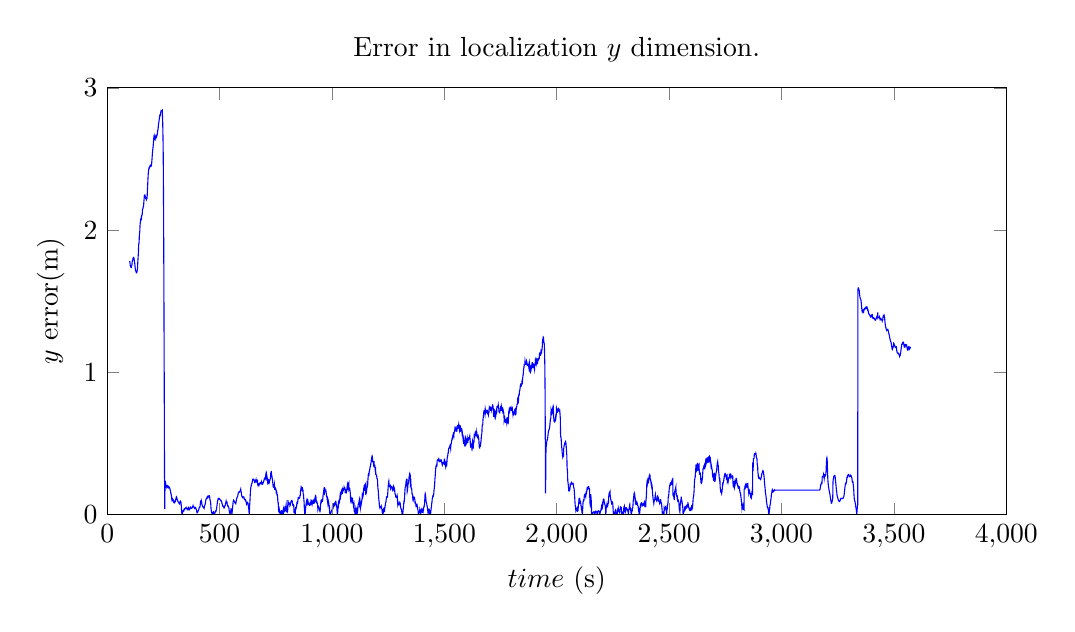
\begin{tikzpicture}

\begin{axis}[
title={Error in localization $y$ dimension.},
xlabel={$time$ (s)},
ylabel={$y$ error(m)},
xmin=0, xmax=4000,
ymin=0, ymax=3,
axis on top,
width=13cm,
height=7cm
]
\addplot [blue]
coordinates {
(100,1.78279283237457)
(101,1.77414169502258)
(102,1.75980498981476)
(103,1.74630990219116)
(104,1.74400446987152)
(105,1.74030087566376)
(106,1.73755810832977)
(107,1.73656575202942)
(108,1.74380175590515)
(109,1.74846915721893)
(110,1.75537745475769)
(111,1.7711391658783)
(112,1.78383483600616)
(113,1.78923942756653)
(114,1.79174878311157)
(115,1.80152721500397)
(116,1.80159504508972)
(117,1.80808003044128)
(118,1.80725864505768)
(119,1.80452303028107)
(120,1.79250816440582)
(121,1.77969698047638)
(122,1.77253937721252)
(123,1.76146149635315)
(124,1.74327039718628)
(125,1.729079246521)
(126,1.7165707988739)
(127,1.7122629327774)
(128,1.71091670227051)
(129,1.70431404209137)
(130,1.69972508049011)
(131,1.70063071346283)
(132,1.70059316253662)
(133,1.71381387996674)
(134,1.71994624423981)
(135,1.72921202468872)
(136,1.77064691734314)
(137,1.7924101228714)
(138,1.82057892036438)
(139,1.84457586956024)
(140,1.89598371696472)
(141,1.90998925876617)
(142,1.91001786899567)
(143,1.96087450790405)
(144,1.97718829917908)
(145,1.98818833637238)
(146,2.02863582801819)
(147,2.0481407327652)
(148,2.06257268619537)
(149,2.07341548633575)
(150,2.07926615905762)
(151,2.07172640991211)
(152,2.07351621818542)
(153,2.10056089019775)
(154,2.1003937587738)
(155,2.10584055042267)
(156,2.11307118988037)
(157,2.14307269477844)
(158,2.14854761981964)
(159,2.15300020599365)
(160,2.16053816509247)
(161,2.16293224525452)
(162,2.17140921783447)
(163,2.19479021263123)
(164,2.21435770225525)
(165,2.23610970211029)
(166,2.24464282226562)
(167,2.24357399177551)
(168,2.24514433574676)
(169,2.23979314994812)
(170,2.22998711299896)
(171,2.223085729599)
(172,2.22458800506592)
(173,2.22675511074066)
(174,2.22807189655304)
(175,2.21725305747986)
(176,2.22252294254303)
(177,2.22332462501526)
(178,2.24317356777191)
(179,2.27862325143814)
(180,2.3091760559082)
(181,2.34536698293686)
(182,2.37948909235001)
(183,2.40224590730667)
(184,2.41380604934692)
(185,2.42956235837936)
(186,2.43630948495865)
(187,2.43472835254669)
(188,2.43967345190048)
(189,2.44358454275131)
(190,2.45062069225311)
(191,2.4539651684761)
(192,2.44952710056305)
(193,2.45137669229507)
(194,2.4500233092308)
(195,2.44777430677414)
(196,2.45058414888382)
(197,2.45601061534882)
(198,2.47255835676193)
(199,2.49008325481415)
(200,2.51368079328537)
(201,2.53425267744064)
(202,2.5525020699501)
(203,2.56893638181686)
(204,2.58314624834061)
(205,2.59947166252136)
(206,2.6197690706253)
(207,2.64052758026123)
(208,2.66220888900757)
(209,2.6660468916893)
(210,2.65377536821365)
(211,2.6387564125061)
(212,2.63765305376053)
(213,2.63535133504868)
(214,2.64439848566055)
(215,2.65357879304886)
(216,2.66024144077301)
(217,2.66503556156158)
(218,2.66296203517914)
(219,2.66460334825516)
(220,2.65771096515655)
(221,2.66484117078781)
(222,2.66757622432709)
(223,2.67602559995651)
(224,2.69137200784683)
(225,2.70088754224777)
(226,2.70765117931366)
(227,2.72016463804245)
(228,2.7421232573986)
(229,2.75103995680809)
(230,2.75888100743294)
(231,2.77221805334091)
(232,2.78305927681923)
(233,2.79345286655426)
(234,2.80533196640015)
(235,2.80331473660469)
(236,2.80833681535721)
(237,2.80870449471474)
(238,2.82333075928688)
(239,2.83374872732162)
(240,2.84018310976028)
(241,2.83923512768745)
(242,2.83698728752136)
(243,2.83739355278015)
(244,2.83779909801483)
(245,2.8403506834507)
(246,2.80265456867218)
(247,2.75714582633972)
(248,2.67667508554459)
(249,2.58635729980469)
(250,2.39505311203003)
(251,2.10640319538116)
(252,1.7203811044693)
(253,1.285872423172)
(254,0.839657747268677)
(255,0.313672029495239)
(256,0.0393772487640378)
(257,0.17007950592041)
(258,0.207602060317993)
(259,0.212910926818847)
(260,0.219676536560058)
(261,0.209763807296753)
(262,0.203025983810425)
(263,0.195897745132446)
(264,0.203431533813477)
(265,0.202725099563599)
(266,0.198888944625855)
(267,0.19732444190979)
(268,0.194191621780396)
(269,0.196744525909424)
(270,0.20113738822937)
(271,0.197807872772217)
(272,0.190159881591797)
(273,0.194188056945801)
(274,0.19513553237915)
(275,0.192460475921631)
(276,0.192544637680053)
(277,0.190209215164185)
(278,0.18600684928894)
(279,0.179689233779907)
(280,0.175427501678467)
(281,0.166262502670288)
(282,0.162306661605835)
(283,0.148803640365601)
(284,0.144348073959351)
(285,0.139269519805908)
(286,0.127996374130249)
(287,0.11100133895874)
(288,0.101406183242798)
(289,0.0955789947509764)
(290,0.0968421363830565)
(291,0.100689058303833)
(292,0.107524518966675)
(293,0.103507495880127)
(294,0.101952529907226)
(295,0.096963144302368)
(296,0.0887611198425291)
(297,0.0916621971130369)
(298,0.0912747669219969)
(299,0.0890235633850098)
(300,0.0858592720031739)
(301,0.0934836597442627)
(302,0.0930503330230712)
(303,0.0916627368927001)
(304,0.0974868259429931)
(305,0.10560259437561)
(306,0.112145515441894)
(307,0.120982023239136)
(308,0.124461124420166)
(309,0.121016691207886)
(310,0.115253398895264)
(311,0.110075424194336)
(312,0.102951139450073)
(313,0.0982023181915283)
(314,0.0978547039031983)
(315,0.0913475456237793)
(316,0.0887912216186524)
(317,0.0881417694091797)
(318,0.0834020080566407)
(319,0.0810097160339356)
(320,0.0796602668762207)
(321,0.0766812267303467)
(322,0.0751117172241211)
(323,0.0837315330505368)
(324,0.088842512130737)
(325,0.0899015674591061)
(326,0.09361794090271)
(327,0.0909645805358887)
(328,0.087281967163086)
(329,0.0742160987854001)
(330,0.054940433502197)
(331,0.0277254295349119)
(332,0.0108556327819822)
(333,0.00121931457519553)
(334,0.00376181030273459)
(335,0.00304378890991197)
(336,0.0182691993713377)
(337,0.022852081298828)
(338,0.028969663619995)
(339,0.0300132217407225)
(340,0.0293237857818602)
(341,0.0266737632751464)
(342,0.0305468730926512)
(343,0.0382175140380858)
(344,0.036206214904785)
(345,0.0378937416076659)
(346,0.0412249259948729)
(347,0.0409824352264403)
(348,0.0415617923736571)
(349,0.0440802078247069)
(350,0.0486514072418211)
(351,0.0505444507598876)
(352,0.0462555389404295)
(353,0.0419322948455809)
(354,0.0420629482269286)
(355,0.040563199996948)
(356,0.0375424365997312)
(357,0.0422893505096433)
(358,0.0422255535125733)
(359,0.0389067668914795)
(360,0.0439068813323975)
(361,0.0484139461517334)
(362,0.0449207229614257)
(363,0.044294635772705)
(364,0.0344682140350341)
(365,0.0324586372375486)
(366,0.0339258651733396)
(367,0.0341950397491453)
(368,0.0388458709716795)
(369,0.0478256740570067)
(370,0.0514074363708494)
(371,0.0526941814422606)
(372,0.0466750659942625)
(373,0.0459652938842772)
(374,0.0447233715057371)
(375,0.0453322925567625)
(376,0.0444816703796387)
(377,0.0470801944732666)
(378,0.0481740589141846)
(379,0.0501833133697511)
(380,0.0536599330902101)
(381,0.0578997306823732)
(382,0.0623531513214113)
(383,0.0559791564941405)
(384,0.0544616222381591)
(385,0.0545124053955077)
(386,0.0506745815277099)
(387,0.0471564769744872)
(388,0.0459925174713134)
(389,0.0432762145996093)
(390,0.0448728504180909)
(391,0.0464538040161133)
(392,0.0499211254119873)
(393,0.048633903503418)
(394,0.0443921794891358)
(395,0.0402708759307861)
(396,0.0359445323944092)
(397,0.0338977279663086)
(398,0.0266016426086426)
(399,0.0180715026855469)
(400,0.021132797241211)
(401,0.0199257869720459)
(402,0.015392972946167)
(403,0.0176960964202881)
(404,0.0212139625549317)
(405,0.0270015735626221)
(406,0.0283574600219727)
(407,0.033255054473877)
(408,0.0379681529998779)
(409,0.0466861667633056)
(410,0.0500109138488769)
(411,0.0506956844329833)
(412,0.0537767677307128)
(413,0.0538900165557861)
(414,0.0695634155273437)
(415,0.0882150230407714)
(416,0.0925041732788085)
(417,0.0885817108154296)
(418,0.0859283504486083)
(419,0.0954214630126953)
(420,0.0888237056732177)
(421,0.0814940032958984)
(422,0.0679937896728515)
(423,0.064635663986206)
(424,0.0593236980438232)
(425,0.0562514362335205)
(426,0.0539016952514646)
(427,0.0512819519042966)
(428,0.0524928798675535)
(429,0.0526709785461423)
(430,0.0474057426452634)
(431,0.0440550079345701)
(432,0.0504055252075193)
(433,0.0597865829467774)
(434,0.0617747554779053)
(435,0.0681789169311524)
(436,0.0727970848083497)
(437,0.0836226177215575)
(438,0.0941113662719726)
(439,0.101795120239258)
(440,0.109672632217407)
(441,0.110609378814697)
(442,0.110660400390625)
(443,0.114334203720093)
(444,0.119512893676758)
(445,0.115227081298828)
(446,0.116570331573486)
(447,0.123451271057129)
(448,0.120204010009766)
(449,0.119550504684448)
(450,0.127976444244385)
(451,0.128231552124023)
(452,0.131745365142822)
(453,0.132725980758667)
(454,0.132345035552978)
(455,0.128480985641479)
(456,0.123921945571899)
(457,0.108022954940796)
(458,0.100182083129883)
(459,0.0940733222961425)
(460,0.0871937541961669)
(461,0.0680882759094237)
(462,0.0429818458557127)
(463,0.0282900161743163)
(464,0.0169129199981688)
(465,0.0146386470794675)
(466,0.00768040084838839)
(467,0.00219868087768527)
(468,0.00681657981872563)
(469,0.00553674888610844)
(470,0.0063840885162354)
(471,0.0167310523986819)
(472,0.0192349243164065)
(473,0.0202856349945071)
(474,0.0142035770416262)
(475,0.00983473205566421)
(476,0.00821968460083022)
(477,0.000435794830322411)
(478,0.00628951072692851)
(479,0.0100362586975096)
(480,0.0144915866851805)
(481,0.0189553031921386)
(482,0.0230043659210204)
(483,0.0217557678222655)
(484,0.0214885005950927)
(485,0.0293070259094237)
(486,0.0355500164031981)
(487,0.0475923004150389)
(488,0.0572911586761475)
(489,0.070112117767334)
(490,0.0818227615356446)
(491,0.0933345642089844)
(492,0.101665386199951)
(493,0.103759178161621)
(494,0.111549028396607)
(495,0.113198226928711)
(496,0.110559648513794)
(497,0.108986562728882)
(498,0.109805734634399)
(499,0.108475358963013)
(500,0.110150249481201)
(501,0.106269987106323)
(502,0.104654939651489)
(503,0.102790029525757)
(504,0.100203426361084)
(505,0.0967256145477293)
(506,0.0962406711578367)
(507,0.0979451255798338)
(508,0.0943872051239012)
(509,0.091819984436035)
(510,0.0825691051483153)
(511,0.0759777851104735)
(512,0.073084575653076)
(513,0.0659060306549071)
(514,0.0601019687652586)
(515,0.0613581962585448)
(516,0.0608551445007324)
(517,0.0576250495910644)
(518,0.055659288406372)
(519,0.0493325328826906)
(520,0.0458366012573244)
(521,0.0479199028015138)
(522,0.0542620754241945)
(523,0.0573709392547608)
(524,0.0634355926513672)
(525,0.0631959819793701)
(526,0.073055631637573)
(527,0.0801037616729734)
(528,0.084814197540283)
(529,0.0933920478820802)
(530,0.0859879589080812)
(531,0.0891229248046876)
(532,0.0898006210327149)
(533,0.085049415588379)
(534,0.0755167255401612)
(535,0.0661580810546876)
(536,0.0590652217864989)
(537,0.058652280807495)
(538,0.059971689224243)
(539,0.0555697479248045)
(540,0.0543261566162108)
(541,0.0487097301483152)
(542,0.0413355636596679)
(543,0.0268318462371826)
(544,0.0187728214263916)
(545,0.0109128761291504)
(546,0.00182964324951174)
(547,0.00716855049133302)
(548,0.0115754795074463)
(549,0.0235150680541993)
(550,0.027422986984253)
(551,0.0396409854888917)
(552,0.0386582241058351)
(553,0.0238631305694579)
(554,0.0124035415649413)
(555,0.00187224769592298)
(556,0.0179321231842042)
(557,0.0356738376617431)
(558,0.0517628002166748)
(559,0.0659551429748535)
(560,0.0820236015319824)
(561,0.0927474308013916)
(562,0.0990114021301269)
(563,0.0958572673797606)
(564,0.0958303260803221)
(565,0.0949713039398192)
(566,0.0946303634643555)
(567,0.0868586330413818)
(568,0.082419755935669)
(569,0.0815205860137937)
(570,0.0801966476440428)
(571,0.0778079319000242)
(572,0.0757877922058103)
(573,0.0839972591400144)
(574,0.0938494300842283)
(575,0.107378253936767)
(576,0.113100919723511)
(577,0.115759525299072)
(578,0.120274457931519)
(579,0.123112098693848)
(580,0.126188652038574)
(581,0.131982223510742)
(582,0.139887706756592)
(583,0.150888666152954)
(584,0.153050168991089)
(585,0.157314762115478)
(586,0.15828667640686)
(587,0.156003580093384)
(588,0.15655909538269)
(589,0.159469947814941)
(590,0.162708541870117)
(591,0.165510913848877)
(592,0.167378446578979)
(593,0.172184886932373)
(594,0.177804174423218)
(595,0.163716259002685)
(596,0.160568656921387)
(597,0.149076404571533)
(598,0.138348760604858)
(599,0.129187049865723)
(600,0.124541702270508)
(601,0.122597398757935)
(602,0.120298805236816)
(603,0.124199741363525)
(604,0.123440616607666)
(605,0.118956678390503)
(606,0.118104093551636)
(607,0.118664754867554)
(608,0.121686710357666)
(609,0.117483631134033)
(610,0.109228626251221)
(611,0.107054725646972)
(612,0.105358139038086)
(613,0.104361471176147)
(614,0.100990232467651)
(615,0.103841003417969)
(616,0.100911508560181)
(617,0.0976816520690917)
(618,0.0890680656433105)
(619,0.0824316310882569)
(620,0.0746355819702149)
(621,0.0795756149291993)
(622,0.0773727779388427)
(623,0.081772792816162)
(624,0.084463108062744)
(625,0.0817465667724608)
(626,0.0802104034423827)
(627,0.0748343029022216)
(628,0.0612852134704589)
(629,0.0486702480316161)
(630,0.0366494216918944)
(631,0.0167729415893554)
(632,0.00236396408081063)
(633,0.0365851440429687)
(634,0.0693729438781738)
(635,0.0922813930511475)
(636,0.122819952011108)
(637,0.154326927185059)
(638,0.175718557357788)
(639,0.190483581542969)
(640,0.197157665252686)
(641,0.20493440246582)
(642,0.209797187805176)
(643,0.215824626922608)
(644,0.220189117431641)
(645,0.225008749008179)
(646,0.233941551208496)
(647,0.245334383010864)
(648,0.247027870178223)
(649,0.249106880187989)
(650,0.24590873336792)
(651,0.245203729629517)
(652,0.244952198028565)
(653,0.244339939117432)
(654,0.238320108413697)
(655,0.239124055862427)
(656,0.224187274932861)
(657,0.223997493743897)
(658,0.226502080917359)
(659,0.233372350692749)
(660,0.234036310195923)
(661,0.241279705047607)
(662,0.24594960975647)
(663,0.233739143371582)
(664,0.229966407775879)
(665,0.231964117050171)
(666,0.237180715560913)
(667,0.240773683547974)
(668,0.241985326766968)
(669,0.240834480285645)
(670,0.208756893157959)
(671,0.204977958679199)
(672,0.214636056900024)
(673,0.215581148147583)
(674,0.212827423095703)
(675,0.21425602722168)
(676,0.209418514251709)
(677,0.215494731903076)
(678,0.218889335632324)
(679,0.215949396133423)
(680,0.217939422607422)
(681,0.216909215927124)
(682,0.222176120758057)
(683,0.220117614746094)
(684,0.218322799682617)
(685,0.223173664093018)
(686,0.222881839752197)
(687,0.230835361480713)
(688,0.225659532546997)
(689,0.213397188186645)
(690,0.212708911895752)
(691,0.213110647201538)
(692,0.222500762939453)
(693,0.223389110565185)
(694,0.222365671157837)
(695,0.222560697555542)
(696,0.232016139984131)
(697,0.23626579284668)
(698,0.242045297622681)
(699,0.249346866607666)
(700,0.254891529083252)
(701,0.255321548461914)
(702,0.258683012008667)
(703,0.260706708908081)
(704,0.256184524536133)
(705,0.274558013916016)
(706,0.282651371002197)
(707,0.263682554244995)
(708,0.268828104019165)
(709,0.277844617843628)
(710,0.259008834838867)
(711,0.265842853546143)
(712,0.25652116394043)
(713,0.250376878738403)
(714,0.222952014923096)
(715,0.216151124954224)
(716,0.218207008361817)
(717,0.228801137924195)
(718,0.242335792541504)
(719,0.240176197052002)
(720,0.229985233306885)
(721,0.223650817871094)
(722,0.228233222961426)
(723,0.236932878494263)
(724,0.243728399276733)
(725,0.248182773590088)
(726,0.254168033599853)
(727,0.270051956176758)
(728,0.292772031784058)
(729,0.299156642913819)
(730,0.300495124816895)
(731,0.285470024108887)
(732,0.275132432937622)
(733,0.26779033279419)
(734,0.255779043197632)
(735,0.248942628860474)
(736,0.235453382492066)
(737,0.21819521522522)
(738,0.20469309425354)
(739,0.193897024154663)
(740,0.192574754714966)
(741,0.200687423706055)
(742,0.196653448104858)
(743,0.203270278930664)
(744,0.211821399688721)
(745,0.174267433166504)
(746,0.184183261871338)
(747,0.189350269317627)
(748,0.187260978698731)
(749,0.182526462554932)
(750,0.179579847335816)
(751,0.173641078948975)
(752,0.155317108154297)
(753,0.15695099067688)
(754,0.159197608947754)
(755,0.139674495697021)
(756,0.136524509429932)
(757,0.138495277404785)
(758,0.132674287796021)
(759,0.0978874874114992)
(760,0.0858707141876223)
(761,0.0834541034698488)
(762,0.0404377803802491)
(763,0.0257268772125245)
(764,0.0176013336181642)
(765,0.0168603286743165)
(766,0.0332420387268066)
(767,0.024510196685791)
(768,0.0120578327178955)
(769,0.00609197425842289)
(770,0.0046642799377441)
(771,0.00964961242675777)
(772,0.0021522178649902)
(773,0.00426055335998532)
(774,0.0201666488647461)
(775,0.0243325366973877)
(776,0.0260623970031739)
(777,0.025048402786255)
(778,0.0220850982666017)
(779,1.37233734132103e-05)
(780,0.0036812877655028)
(781,0.0113171195983885)
(782,0.0223606681823729)
(783,0.0324948196411134)
(784,0.0382466678619386)
(785,0.0443551902770998)
(786,0.0203715438842775)
(787,0.0253664131164553)
(788,0.0234194869995119)
(789,0.0310376758575441)
(790,0.0350056571960451)
(791,0.0414608402252199)
(792,0.0563505573272707)
(793,0.0221444568634035)
(794,0.0357924900054933)
(795,0.0535985431671144)
(796,0.0652851066589357)
(797,0.0431559753417967)
(798,0.0493295860290526)
(799,0.0492971611022948)
(800,0.0183660717010499)
(801,0.0159361095428467)
(802,0.0185019702911378)
(803,0.0264670581817628)
(804,0.102802236557007)
(805,0.0739016132354737)
(806,0.0713955955505372)
(807,0.0763475494384766)
(808,0.0786625938415528)
(809,0.0809912281036378)
(810,0.0761708831787109)
(811,0.0766050434112548)
(812,0.0768990135192871)
(813,0.0607343521118167)
(814,0.063171943664551)
(815,0.0694163646698)
(816,0.0798028316497805)
(817,0.0834912662506104)
(818,0.0939471130371094)
(819,0.0959064369201661)
(820,0.0976301651000977)
(821,0.0978423576354981)
(822,0.0989762763977051)
(823,0.0956405620574951)
(824,0.0823722896575929)
(825,0.0770510253906251)
(826,0.0623866138458253)
(827,0.0620958404541017)
(828,0.0647921161651612)
(829,0.0671407775878907)
(830,0.0636434154510499)
(831,0.0196995677947998)
(832,0.0209357681274414)
(833,0.0208060684204101)
(834,0.0243256034851074)
(835,0.00421466064453124)
(836,0.00355591011047363)
(837,0.00666366386413575)
(838,0.0462076530456543)
(839,0.051012264251709)
(840,0.0520791873931885)
(841,0.0470280399322509)
(842,0.0536024322509765)
(843,0.0589956989288329)
(844,0.086043119430542)
(845,0.0867764949798584)
(846,0.0791411399841308)
(847,0.0789499282836914)
(848,0.0951367549896238)
(849,0.105265491485595)
(850,0.119706504821777)
(851,0.120266986846924)
(852,0.117860151290893)
(853,0.114112449645996)
(854,0.113341329574585)
(855,0.118597743988037)
(856,0.11980700302124)
(857,0.120362461090088)
(858,0.135861814498901)
(859,0.136356294631958)
(860,0.163583734512329)
(861,0.172407844543457)
(862,0.178012588500977)
(863,0.1919967918396)
(864,0.187569965362549)
(865,0.175128568649292)
(866,0.172561515808105)
(867,0.190331523895264)
(868,0.189718788146973)
(869,0.183853452682495)
(870,0.174446022033691)
(871,0.169881021499634)
(872,0.146311199188232)
(873,0.144572689056397)
(874,0.122789813995361)
(875,0.105014516830444)
(876,0.0892517108917237)
(877,0.0492349319458007)
(878,0.0279076747894287)
(879,0.00174505043029782)
(880,0.00981938934326187)
(881,0.00993287467956527)
(882,0.0325249423980711)
(883,0.0469626178741453)
(884,0.0616315727233889)
(885,0.0711773757934573)
(886,0.0828796749114993)
(887,0.0629595279693604)
(888,0.0763882160186768)
(889,0.0812679290771485)
(890,0.0967140827178956)
(891,0.0988181266784669)
(892,0.104378286361694)
(893,0.10148436164856)
(894,0.0721167850494386)
(895,0.0736524391174318)
(896,0.0759736824035646)
(897,0.0750445365905761)
(898,0.0777377128601073)
(899,0.0685960292816161)
(900,0.0635407295227051)
(901,0.0628931846618652)
(902,0.0650461044311523)
(903,0.0704596366882324)
(904,0.0725003795623782)
(905,0.0806299762725833)
(906,0.0894075946807864)
(907,0.0827361736297609)
(908,0.0922476444244387)
(909,0.095257917404175)
(910,0.078613025665283)
(911,0.0805744953155516)
(912,0.0733494586944578)
(913,0.0814015693664549)
(914,0.085463966369629)
(915,0.0940782680511476)
(916,0.0968510761260988)
(917,0.0794438610076904)
(918,0.0795182476043701)
(919,0.0839401969909668)
(920,0.0877323818206785)
(921,0.0942462158203123)
(922,0.100315637588501)
(923,0.106411046981811)
(924,0.0939931735992432)
(925,0.10064409828186)
(926,0.108916984558105)
(927,0.132274745941162)
(928,0.13062727355957)
(929,0.121591209411621)
(930,0.093725503921509)
(931,0.0847466602325442)
(932,0.0827389373779299)
(933,0.0866206302642824)
(934,0.0791188659667967)
(935,0.0789092960357664)
(936,0.0769647541046141)
(937,0.0465791950225829)
(938,0.0564046630859374)
(939,0.0586541423797606)
(940,0.0562544918060301)
(941,0.0512438869476317)
(942,0.048441753387451)
(943,0.0366900596618653)
(944,0.0402048263549806)
(945,0.0377627048492433)
(946,0.0282135639190675)
(947,0.0159016227722168)
(948,0.0398035621643067)
(949,0.0673819160461426)
(950,0.0762445411682129)
(951,0.0902361354827881)
(952,0.0866238555908203)
(953,0.085890718460083)
(954,0.0978359279632568)
(955,0.0946029720306396)
(956,0.0910769996643066)
(957,0.0916350097656249)
(958,0.0994367809295653)
(959,0.108624956130981)
(960,0.12650849533081)
(961,0.140861532211304)
(962,0.147324583053589)
(963,0.161074897766113)
(964,0.151464960098266)
(965,0.147994539260864)
(966,0.145645401000976)
(967,0.1926314868927)
(968,0.181086067199707)
(969,0.169279579162597)
(970,0.173499568939209)
(971,0.168230756759644)
(972,0.16351078414917)
(973,0.166376939773559)
(974,0.156021705627441)
(975,0.144703022003174)
(976,0.128467948913574)
(977,0.126142175674438)
(978,0.117619188308716)
(979,0.106438133239746)
(980,0.0944168300628663)
(981,0.0835842819213868)
(982,0.107808549880982)
(983,0.101694067001343)
(984,0.0944981174468995)
(985,0.0883111553192139)
(986,0.0776884632110595)
(987,0.0578091220855712)
(988,0.0442786293029784)
(989,0.047839380264282)
(990,0.0117308864593504)
(991,0.00345418548583964)
(992,0.00428916740417495)
(993,0.00627161788940445)
(994,0.000635845184326023)
(995,0.0051820449829103)
(996,0.0181586914062501)
(997,0.0235779457092287)
(998,0.0259459190368654)
(999,0.0289182548522948)
(1000,0.0271763687133788)
(1001,0.0274288539886474)
(1002,0.0522429466247556)
(1003,0.0503124713897702)
(1004,0.0448183536529538)
(1005,0.0436412811279294)
(1006,0.0598260707855225)
(1007,0.06794970703125)
(1008,0.0750309772491455)
(1009,0.0776674098968506)
(1010,0.0787395782470703)
(1011,0.0678891487121582)
(1012,0.0640720672607422)
(1013,0.0774809055328367)
(1014,0.0824671916961668)
(1015,0.0828827552795408)
(1016,0.0918274135589598)
(1017,0.0928058834075926)
(1018,0.0837059230804442)
(1019,0.0686705322265624)
(1020,0.0662849159240721)
(1021,0.0587659091949462)
(1022,0.0421717376708983)
(1023,0.0210104198455809)
(1024,0.00184061241149891)
(1025,0.00787732887268078)
(1026,0.0243260650634767)
(1027,0.0477490215301515)
(1028,0.0694660930633546)
(1029,0.0651051311492918)
(1030,0.0870670585632323)
(1031,0.104079177856445)
(1032,0.0886359100341796)
(1033,0.0861446743011473)
(1034,0.0982742195129393)
(1035,0.111834276199341)
(1036,0.132659662246704)
(1037,0.145696628570557)
(1038,0.149863708496094)
(1039,0.134295146942139)
(1040,0.144945781707764)
(1041,0.156587045669556)
(1042,0.163134735107422)
(1043,0.148243432998657)
(1044,0.150378471374512)
(1045,0.146856552124023)
(1046,0.147693639755249)
(1047,0.157222038269043)
(1048,0.180330282211304)
(1049,0.176850648880005)
(1050,0.175768228530884)
(1051,0.172713132858276)
(1052,0.179146747589111)
(1053,0.181284408569336)
(1054,0.19132493019104)
(1055,0.185707788467407)
(1056,0.187978248596191)
(1057,0.187886457443237)
(1058,0.179073553085327)
(1059,0.150480083465576)
(1060,0.164882472991943)
(1061,0.178704074859619)
(1062,0.15268399810791)
(1063,0.151408220291138)
(1064,0.151708389282227)
(1065,0.167670989990234)
(1066,0.171856378555298)
(1067,0.187854026794433)
(1068,0.199846242904663)
(1069,0.212063287734985)
(1070,0.204964374542236)
(1071,0.193556999206543)
(1072,0.203335021972656)
(1073,0.193144508361816)
(1074,0.212758728027344)
(1075,0.218041964530945)
(1076,0.176078934669495)
(1077,0.179793138504028)
(1078,0.18312837600708)
(1079,0.182414908409119)
(1080,0.170009632110596)
(1081,0.155485887527466)
(1082,0.147898693084717)
(1083,0.0956047821044921)
(1084,0.0908271121978759)
(1085,0.101423387527466)
(1086,0.108766202926636)
(1087,0.112392072677612)
(1088,0.107331399917602)
(1089,0.109517698287964)
(1090,0.0946466445922853)
(1091,0.100973320007324)
(1092,0.104711842536926)
(1093,0.0892447309494018)
(1094,0.0836746768951415)
(1095,0.0772283153533935)
(1096,0.0604935512542726)
(1097,0.0648090467453004)
(1098,0.0717693195343019)
(1099,0.0311509075164795)
(1100,0.0332619848251343)
(1101,0.0219502153396607)
(1102,0.0258847179412842)
(1103,0.0121523237228394)
(1104,0.0259649848937988)
(1105,0.0350992774963379)
(1106,0.0110421638488769)
(1107,0.00650040912628169)
(1108,0.00018148231506343)
(1109,0.0263566026687623)
(1110,0.0395120630264283)
(1111,0.0456794748306275)
(1112,0.0453167209625245)
(1113,0.0113557949066163)
(1114,0.0179818048477174)
(1115,0.0356088056564332)
(1116,0.0582402954101562)
(1117,0.0710753211975097)
(1118,0.0770580778121947)
(1119,0.0804803380966186)
(1120,0.0828626165390014)
(1121,0.095814109802246)
(1122,0.10313725566864)
(1123,0.0753388433456421)
(1124,0.0831564693450928)
(1125,0.0920115737915039)
(1126,0.0765693216323853)
(1127,0.0466833534240723)
(1128,0.0557951154708862)
(1129,0.0625505867004394)
(1130,0.0707687215805055)
(1131,0.0792507009506227)
(1132,0.0954533891677858)
(1133,0.0954341964721681)
(1134,0.112441547393799)
(1135,0.142273672103882)
(1136,0.154270656585693)
(1137,0.121961720466614)
(1138,0.126414187431336)
(1139,0.136269934654236)
(1140,0.153858758926392)
(1141,0.17459247303009)
(1142,0.189797021865845)
(1143,0.198204376220703)
(1144,0.205265261650085)
(1145,0.206339337348938)
(1146,0.20853874874115)
(1147,0.166309338569641)
(1148,0.184985500335693)
(1149,0.193821531295776)
(1150,0.143092956542969)
(1151,0.14205500125885)
(1152,0.157408323287964)
(1153,0.155250510215759)
(1154,0.165679892539978)
(1155,0.184776863098145)
(1156,0.20622785949707)
(1157,0.195354319572449)
(1158,0.201419807434082)
(1159,0.211628056526184)
(1160,0.241119003295898)
(1161,0.267939305305481)
(1162,0.284462666511536)
(1163,0.287349319458008)
(1164,0.26884877204895)
(1165,0.28344952583313)
(1166,0.303055758476257)
(1167,0.306006936073303)
(1168,0.316051033973694)
(1169,0.326590088844299)
(1170,0.337036279678345)
(1171,0.338282374382019)
(1172,0.344440964698792)
(1173,0.361218956947327)
(1174,0.364554424285889)
(1175,0.380811948776245)
(1176,0.390011210441589)
(1177,0.369744468688965)
(1178,0.38683037853241)
(1179,0.396367121696472)
(1180,0.401493597984314)
(1181,0.376337141036987)
(1182,0.371905535697937)
(1183,0.367636174201965)
(1184,0.362520307540894)
(1185,0.352680323600769)
(1186,0.360417006492615)
(1187,0.37708890247345)
(1188,0.3486349401474)
(1189,0.336264115333557)
(1190,0.334745269775391)
(1191,0.337617021560669)
(1192,0.32099418258667)
(1193,0.326993747711182)
(1194,0.32803718662262)
(1195,0.282112408638)
(1196,0.281308818817139)
(1197,0.2783681640625)
(1198,0.274565864562988)
(1199,0.271713921546936)
(1200,0.253956267356872)
(1201,0.252170154571533)
(1202,0.248438903808594)
(1203,0.235661575317383)
(1204,0.194805724143982)
(1205,0.180114728927612)
(1206,0.167739731788635)
(1207,0.137867115974426)
(1208,0.117694519996643)
(1209,0.100168847084045)
(1210,0.0865760078430175)
(1211,0.063811873435974)
(1212,0.0529395093917846)
(1213,0.0476617565155029)
(1214,0.0545482234954835)
(1215,0.0548655586242677)
(1216,0.0493715600967408)
(1217,0.0486317472457887)
(1218,0.0574006576538086)
(1219,0.0613305110931397)
(1220,0.0558986206054688)
(1221,0.0458872509002686)
(1222,0.0371666145324707)
(1223,0.0287521076202393)
(1224,0.0126146793365478)
(1225,0.00362164974212642)
(1226,0.000647139549255327)
(1227,0.00617594718933101)
(1228,0.0346922492980957)
(1229,0.0354439830780029)
(1230,0.0388103342056274)
(1231,0.0199395961761475)
(1232,0.0224613494873047)
(1233,0.0298387355804444)
(1234,0.0274462051391602)
(1235,0.0406370372772218)
(1236,0.0530636520385743)
(1237,0.0617794008255006)
(1238,0.0785992212295532)
(1239,0.0833144254684448)
(1240,0.0852474040985107)
(1241,0.10378361415863)
(1242,0.11434775352478)
(1243,0.124369201660156)
(1244,0.125829753875732)
(1245,0.125448999404907)
(1246,0.125306544303894)
(1247,0.124134240150452)
(1248,0.143330869674683)
(1249,0.16906994342804)
(1250,0.189805445671082)
(1251,0.212299825668335)
(1252,0.22559082698822)
(1253,0.233355404853821)
(1254,0.212582111358643)
(1255,0.201612591743469)
(1256,0.199655294418335)
(1257,0.196252107620239)
(1258,0.193643808364868)
(1259,0.191389799118042)
(1260,0.197006225585937)
(1261,0.18467165184021)
(1262,0.1909555311203)
(1263,0.192161213874817)
(1264,0.197649132728577)
(1265,0.197117521286011)
(1266,0.19613332939148)
(1267,0.190049125671387)
(1268,0.182268931388855)
(1269,0.188353254318237)
(1270,0.186785890579224)
(1271,0.176807238578796)
(1272,0.182275368690491)
(1273,0.185103370666504)
(1274,0.198137237548828)
(1275,0.194376661300659)
(1276,0.18095405292511)
(1277,0.185948683738709)
(1278,0.180419041633606)
(1279,0.170007898330688)
(1280,0.151090695381165)
(1281,0.144352628707886)
(1282,0.14019854259491)
(1283,0.133040859222412)
(1284,0.122099115371704)
(1285,0.122036053657532)
(1286,0.120182468414307)
(1287,0.120808078765869)
(1288,0.119736148834229)
(1289,0.126222922325134)
(1290,0.132766081809998)
(1291,0.122766568183899)
(1292,0.088286184310913)
(1293,0.0692942371368408)
(1294,0.0754997959136963)
(1295,0.0817572107315063)
(1296,0.0765080194473266)
(1297,0.0732055644989014)
(1298,0.0700444917678833)
(1299,0.0741998901367187)
(1300,0.0775655260086059)
(1301,0.0769844999313354)
(1302,0.0847497930526733)
(1303,0.0808219661712646)
(1304,0.0745093574523925)
(1305,0.0559501399993896)
(1306,0.0459925880432128)
(1307,0.044070457458496)
(1308,0.0363734712600707)
(1309,0.0364576330184936)
(1310,0.0286085357666015)
(1311,0.0149557342529296)
(1312,0.0049665918350219)
(1313,0.00128903484344489)
(1314,0.00653281307220466)
(1315,0.00542273616790778)
(1316,0.0198654184341431)
(1317,0.038405800819397)
(1318,0.0485358486175538)
(1319,0.0700710067749024)
(1320,0.0884425888061524)
(1321,0.086433060646057)
(1322,0.0963285045623778)
(1323,0.11691523361206)
(1324,0.151442786216736)
(1325,0.177353163719177)
(1326,0.192522784233093)
(1327,0.194501658439636)
(1328,0.200409313201904)
(1329,0.222275992393494)
(1330,0.233142157554626)
(1331,0.241705318450928)
(1332,0.246330996513367)
(1333,0.248170753479004)
(1334,0.246054907798767)
(1335,0.164160890579224)
(1336,0.172100110054016)
(1337,0.186774773597717)
(1338,0.205586357116699)
(1339,0.216118140220642)
(1340,0.218868179321289)
(1341,0.225222868919372)
(1342,0.244103593826294)
(1343,0.260938925743103)
(1344,0.268178625106811)
(1345,0.283407731056213)
(1346,0.288608474731445)
(1347,0.282006664276123)
(1348,0.281918807029724)
(1349,0.216634459495544)
(1350,0.222873516082764)
(1351,0.22828275680542)
(1352,0.191007394790649)
(1353,0.182441253662109)
(1354,0.18313898563385)
(1355,0.178074975013733)
(1356,0.150498595237732)
(1357,0.141501870155334)
(1358,0.138232793807983)
(1359,0.139499988555908)
(1360,0.101347818374634)
(1361,0.0975366973876952)
(1362,0.108177556991577)
(1363,0.121191625595093)
(1364,0.122054104804993)
(1365,0.117961888313293)
(1366,0.120467667579651)
(1367,0.118013178825378)
(1368,0.110466992378235)
(1369,0.101120984077454)
(1370,0.0766625452041625)
(1371,0.0753220367431639)
(1372,0.0790349292755126)
(1373,0.0726931142807006)
(1374,0.0574264755249023)
(1375,0.0584546556472778)
(1376,0.0686383476257324)
(1377,0.0660127773284911)
(1378,0.0593816413879393)
(1379,0.0638440027236937)
(1380,0.054437078475952)
(1381,0.044044651031494)
(1382,0.034895218849182)
(1383,0.0270966663360594)
(1384,0.0109993419647216)
(1385,0.0153448781967163)
(1386,0.010638614654541)
(1387,0.0127704629898071)
(1388,0.0125258455276489)
(1389,0.0194842109680176)
(1390,0.020336199760437)
(1391,0.0366475095748902)
(1392,0.030219744682312)
(1393,0.0180413236618042)
(1394,0.00954085731506349)
(1395,0.0171038522720337)
(1396,0.0129304542541504)
(1397,0.0176075115203858)
(1398,0.0312964458465577)
(1399,0.0372944612503052)
(1400,0.0405894060134888)
(1401,0.037127492904663)
(1402,0.0282021741867064)
(1403,0.015873191833496)
(1404,0.0129330606460571)
(1405,0.0125526638031006)
(1406,0.02479700756073)
(1407,0.0322885065078735)
(1408,0.0459123401641845)
(1409,0.0568166522979736)
(1410,0.0559192447662353)
(1411,0.0603774652481079)
(1412,0.0740954742431641)
(1413,0.105310903549194)
(1414,0.138397610664368)
(1415,0.146768248558044)
(1416,0.140913522720337)
(1417,0.123507416725159)
(1418,0.106628414154053)
(1419,0.090702410697937)
(1420,0.0837291440963745)
(1421,0.0805034666061401)
(1422,0.0726947813034058)
(1423,0.0598852663040161)
(1424,0.0546710653305054)
(1425,0.0455296201705932)
(1426,0.0317229194641113)
(1427,0.0129563970565796)
(1428,0.00615409278869627)
(1429,0.0264981117248535)
(1430,0.0312971200942993)
(1431,0.0363492031097412)
(1432,0.0376806516647339)
(1433,0.0342685241699219)
(1434,0.0131412830352784)
(1435,0.0202894296646119)
(1436,0.0221798505783082)
(1437,0.00186841869354248)
(1438,0.00152999973297119)
(1439,0.00758404350280761)
(1440,0.025016152381897)
(1441,0.0363372201919556)
(1442,0.0504326457977295)
(1443,0.0618762607574463)
(1444,0.0804276132583617)
(1445,0.088987317085266)
(1446,0.108139481544494)
(1447,0.114733468055725)
(1448,0.121615420341492)
(1449,0.133342038154602)
(1450,0.135347496032715)
(1451,0.131578010559082)
(1452,0.136619967460632)
(1453,0.146021288871765)
(1454,0.169032047271728)
(1455,0.18266362953186)
(1456,0.196744392395019)
(1457,0.217759321212768)
(1458,0.247224810600281)
(1459,0.262868288040161)
(1460,0.286324265480041)
(1461,0.312496675491333)
(1462,0.329047216415405)
(1463,0.340962065696716)
(1464,0.344249459266662)
(1465,0.336899014472961)
(1466,0.336783381462097)
(1467,0.344264718055725)
(1468,0.376907134056091)
(1469,0.382064366340637)
(1470,0.381138467788696)
(1471,0.384843411445618)
(1472,0.386026086807251)
(1473,0.38259512424469)
(1474,0.387552680969238)
(1475,0.391222811698914)
(1476,0.383720255851746)
(1477,0.37905380821228)
(1478,0.373261905670166)
(1479,0.370977390289306)
(1480,0.371201622962952)
(1481,0.372117388725281)
(1482,0.381600558280945)
(1483,0.379441082000732)
(1484,0.381402432441711)
(1485,0.38183941078186)
(1486,0.376331822395325)
(1487,0.37931050491333)
(1488,0.371389013290405)
(1489,0.361379962921142)
(1490,0.352976661682129)
(1491,0.347639304161072)
(1492,0.352688099861145)
(1493,0.358271982192993)
(1494,0.363887097358704)
(1495,0.362688738822937)
(1496,0.361185748100281)
(1497,0.365072447776794)
(1498,0.361318308830261)
(1499,0.376026001930237)
(1500,0.388217655181885)
(1501,0.388958064079285)
(1502,0.374275173187256)
(1503,0.363530720710754)
(1504,0.35205730342865)
(1505,0.343722547531128)
(1506,0.373548285484314)
(1507,0.362810627937317)
(1508,0.353630916595459)
(1509,0.348854418754578)
(1510,0.343592759132385)
(1511,0.349054213523865)
(1512,0.383748517990112)
(1513,0.400731431007385)
(1514,0.40830122089386)
(1515,0.411853180885315)
(1516,0.426050430297852)
(1517,0.435538059234619)
(1518,0.435263401031494)
(1519,0.462393755912781)
(1520,0.46562087059021)
(1521,0.467094058990478)
(1522,0.472041300773621)
(1523,0.470511845588684)
(1524,0.477740816116333)
(1525,0.483389190673828)
(1526,0.47705380821228)
(1527,0.47757666015625)
(1528,0.466393040657043)
(1529,0.490021290779114)
(1530,0.494195761680603)
(1531,0.5018577003479)
(1532,0.511147918701172)
(1533,0.520614305496216)
(1534,0.530718961715698)
(1535,0.529970804214477)
(1536,0.543784133911133)
(1537,0.551956169128418)
(1538,0.556595437049866)
(1539,0.56219898891449)
(1540,0.552872968673706)
(1541,0.556015206336975)
(1542,0.549445582389831)
(1543,0.573432868957519)
(1544,0.578799075126648)
(1545,0.584509438514709)
(1546,0.589238709449768)
(1547,0.603629592895508)
(1548,0.59758115196228)
(1549,0.601382736206055)
(1550,0.601217864990234)
(1551,0.606160401344299)
(1552,0.598250149726868)
(1553,0.58586740398407)
(1554,0.586737112045288)
(1555,0.591429904937744)
(1556,0.58984394454956)
(1557,0.611410007476806)
(1558,0.624140486717224)
(1559,0.622683868408203)
(1560,0.616064534187317)
(1561,0.611952408790588)
(1562,0.616910442352295)
(1563,0.625814064979553)
(1564,0.634466472625732)
(1565,0.623988333702087)
(1566,0.609043661117553)
(1567,0.599173370361328)
(1568,0.625626573562622)
(1569,0.625239262580871)
(1570,0.623098859786987)
(1571,0.621749829292297)
(1572,0.613738607406616)
(1573,0.587522815704346)
(1574,0.588746856689453)
(1575,0.604488426208496)
(1576,0.603977256774902)
(1577,0.603790098190307)
(1578,0.583636999130249)
(1579,0.567896366119385)
(1580,0.549107074737549)
(1581,0.563635553359985)
(1582,0.551908697128296)
(1583,0.539035881996155)
(1584,0.517456258773804)
(1585,0.508792133331299)
(1586,0.49829122543335)
(1587,0.498009653091431)
(1588,0.525632599830627)
(1589,0.516035894393921)
(1590,0.501730660438538)
(1591,0.485127824783325)
(1592,0.481134313583374)
(1593,0.481845039367676)
(1594,0.483251112937927)
(1595,0.533941122055054)
(1596,0.527587743759155)
(1597,0.517867060661316)
(1598,0.511127205848694)
(1599,0.52591268825531)
(1600,0.527809784889221)
(1601,0.520155475616455)
(1602,0.533444629669189)
(1603,0.520534978866577)
(1604,0.504531012535095)
(1605,0.526287599563599)
(1606,0.527600451469421)
(1607,0.532988711357117)
(1608,0.529706998825073)
(1609,0.534254406929016)
(1610,0.540435170173645)
(1611,0.543516134262085)
(1612,0.545616721153259)
(1613,0.551668782234192)
(1614,0.534496803283691)
(1615,0.517921586036682)
(1616,0.484934741020202)
(1617,0.476206952095032)
(1618,0.478311234474182)
(1619,0.49561944770813)
(1620,0.490732939720154)
(1621,0.484788330078125)
(1622,0.471815259933472)
(1623,0.479410248756409)
(1624,0.465267616271973)
(1625,0.472680645942688)
(1626,0.511005933761597)
(1627,0.502591426849365)
(1628,0.486988599777222)
(1629,0.480968649864197)
(1630,0.513796160697937)
(1631,0.519020030975342)
(1632,0.51734323310852)
(1633,0.550480173110962)
(1634,0.545408890724182)
(1635,0.543224857330322)
(1636,0.548153207778931)
(1637,0.577449255943298)
(1638,0.581373029708862)
(1639,0.577410155296326)
(1640,0.57078439617157)
(1641,0.570005721092224)
(1642,0.557592457771301)
(1643,0.555193966865539)
(1644,0.578073001861572)
(1645,0.566975451469421)
(1646,0.553159571647644)
(1647,0.545491827011108)
(1648,0.548520339012146)
(1649,0.544442904472351)
(1650,0.540367496490478)
(1651,0.55033695602417)
(1652,0.544590949058533)
(1653,0.530722617149353)
(1654,0.512112258911133)
(1655,0.475945105552673)
(1656,0.472832908630371)
(1657,0.470078458786011)
(1658,0.482036838531494)
(1659,0.477947721481323)
(1660,0.478492150306702)
(1661,0.482476959228516)
(1662,0.50803928565979)
(1663,0.513276268959045)
(1664,0.532401849746704)
(1665,0.555923147201538)
(1666,0.564883275032043)
(1667,0.567810459136963)
(1668,0.613351480484009)
(1669,0.627545969009399)
(1670,0.634091512680054)
(1671,0.634695546150207)
(1672,0.67055553150177)
(1673,0.680972277641296)
(1674,0.689511835098267)
(1675,0.718434788703918)
(1676,0.722929098129272)
(1677,0.731018044471741)
(1678,0.730556108474731)
(1679,0.729047048568725)
(1680,0.72118305015564)
(1681,0.711067426681518)
(1682,0.741348196983337)
(1683,0.732702066421509)
(1684,0.721261193275452)
(1685,0.716462304115295)
(1686,0.721273323059082)
(1687,0.720770379066467)
(1688,0.720074912071228)
(1689,0.731484159469604)
(1690,0.730803593635559)
(1691,0.726272806167602)
(1692,0.717532738685608)
(1693,0.722526869773865)
(1694,0.709268293380737)
(1695,0.710002980232239)
(1696,0.702135524749756)
(1697,0.71659653377533)
(1698,0.715896059989929)
(1699,0.723648359298706)
(1700,0.750353660583496)
(1701,0.745748248100281)
(1702,0.746326413154602)
(1703,0.746752109527588)
(1704,0.753493650436401)
(1705,0.749813659667969)
(1706,0.728901489257812)
(1707,0.743649379730224)
(1708,0.743469612121582)
(1709,0.743094818115234)
(1710,0.735473768234253)
(1711,0.750951312065124)
(1712,0.750365636825561)
(1713,0.751873991966247)
(1714,0.770160787582397)
(1715,0.770864480018616)
(1716,0.763820164680481)
(1717,0.757516496658325)
(1718,0.727999662399292)
(1719,0.700473879814148)
(1720,0.68657860660553)
(1721,0.724368085861206)
(1722,0.719113698005676)
(1723,0.705072393417358)
(1724,0.719697691917419)
(1725,0.709917523384094)
(1726,0.696778752326965)
(1727,0.689531781196594)
(1728,0.7195170545578)
(1729,0.716898503303528)
(1730,0.708990278244018)
(1731,0.722294129371643)
(1732,0.714638270378113)
(1733,0.719931878089905)
(1734,0.757860175132751)
(1735,0.75929092502594)
(1736,0.752913228034973)
(1737,0.754239789009094)
(1738,0.757828346252441)
(1739,0.758078328132629)
(1740,0.769365326881409)
(1741,0.756885663986206)
(1742,0.747657315254211)
(1743,0.72413255405426)
(1744,0.723904897689819)
(1745,0.717858364105224)
(1746,0.716132690429687)
(1747,0.725496718406677)
(1748,0.728973695755005)
(1749,0.730706045150757)
(1750,0.748171424865723)
(1751,0.745536184310913)
(1752,0.759949660301208)
(1753,0.765427229881286)
(1754,0.745619891166687)
(1755,0.729724882125854)
(1756,0.756406840324402)
(1757,0.743795928001404)
(1758,0.735211190223694)
(1759,0.739176433563232)
(1760,0.72278241443634)
(1761,0.709683101654053)
(1762,0.730993176460266)
(1763,0.724098230361938)
(1764,0.715967322349548)
(1765,0.705062414169311)
(1766,0.663393739700317)
(1767,0.672434929847717)
(1768,0.668396357536316)
(1769,0.674279096603393)
(1770,0.663975241661072)
(1771,0.652413132667541)
(1772,0.647879183769226)
(1773,0.646975338935852)
(1774,0.649061263084411)
(1775,0.662058518409729)
(1776,0.666698382377624)
(1777,0.656859324455261)
(1778,0.64368258523941)
(1779,0.655693878173828)
(1780,0.644272376537323)
(1781,0.643771518707275)
(1782,0.66777401971817)
(1783,0.66396873998642)
(1784,0.668182073116302)
(1785,0.661298809528351)
(1786,0.715737642288208)
(1787,0.725473822593689)
(1788,0.732459069728851)
(1789,0.742738891601562)
(1790,0.737536657810211)
(1791,0.728558648586273)
(1792,0.73720030260086)
(1793,0.738654119491577)
(1794,0.747781915187836)
(1795,0.743752223968506)
(1796,0.745003787517547)
(1797,0.735631553173065)
(1798,0.733524827003479)
(1799,0.735804627418518)
(1800,0.742668579101562)
(1801,0.754774938106537)
(1802,0.751917074203491)
(1803,0.728037227630615)
(1804,0.718344797134399)
(1805,0.70663916015625)
(1806,0.723413306713104)
(1807,0.720832127571106)
(1808,0.720126885414123)
(1809,0.709431845188141)
(1810,0.703720084190369)
(1811,0.705437472820282)
(1812,0.710975638389587)
(1813,0.736946344852447)
(1814,0.73910719203949)
(1815,0.725566864490509)
(1816,0.711684335708618)
(1817,0.703419436454773)
(1818,0.704799403190613)
(1819,0.714380074977875)
(1820,0.751550026893616)
(1821,0.757333286762237)
(1822,0.757777281761169)
(1823,0.771061342716217)
(1824,0.775523286819458)
(1825,0.779031795024872)
(1826,0.786737066268921)
(1827,0.824512978076935)
(1828,0.82558896112442)
(1829,0.820211012840271)
(1830,0.810456533908844)
(1831,0.836437772750854)
(1832,0.843071352481842)
(1833,0.841904412746429)
(1834,0.864697372436523)
(1835,0.868457471847534)
(1836,0.876067256450653)
(1837,0.887513732433319)
(1838,0.904151353359222)
(1839,0.910596105575561)
(1840,0.918134185791015)
(1841,0.918060962200165)
(1842,0.913804475307464)
(1843,0.908227149486542)
(1844,0.912512246608734)
(1845,0.928505780696869)
(1846,0.922894599437713)
(1847,0.922048809528351)
(1848,0.952600473880768)
(1849,0.963593835353851)
(1850,0.978858704090118)
(1851,0.985252732753754)
(1852,1.01324116611481)
(1853,1.02615606212616)
(1854,1.02876114273071)
(1855,1.05214265346527)
(1856,1.0507185792923)
(1857,1.05330494403839)
(1858,1.05400720596313)
(1859,1.08025834083557)
(1860,1.07141837596893)
(1861,1.07038864612579)
(1862,1.06255355596542)
(1863,1.06439385318756)
(1864,1.06008920574188)
(1865,1.06288120651245)
(1866,1.07799353837967)
(1867,1.07264509439468)
(1868,1.05684437990189)
(1869,1.04793867111206)
(1870,1.04874319171906)
(1871,1.05151355600357)
(1872,1.05651820039749)
(1873,1.05566567516327)
(1874,1.05300989723206)
(1875,1.04269435977936)
(1876,1.03305575227737)
(1877,1.0626839132309)
(1878,1.0712253780365)
(1879,1.05649796438217)
(1880,1.04156074237823)
(1881,1.01005769300461)
(1882,1.00393403100967)
(1883,1.00095975923538)
(1884,1.04279131698608)
(1885,1.04475087928772)
(1886,1.04127181577682)
(1887,1.03065533447266)
(1888,1.04083972644806)
(1889,1.0322366900444)
(1890,1.03192215633392)
(1891,1.07140207242966)
(1892,1.06050509166717)
(1893,1.04694515419006)
(1894,1.03173196268082)
(1895,1.05559168481827)
(1896,1.05725662136078)
(1897,1.05451135063171)
(1898,1.05501137399673)
(1899,1.04406615304947)
(1900,1.0286467294693)
(1901,1.02028765487671)
(1902,1.04511523246765)
(1903,1.05351370573044)
(1904,1.05381655693054)
(1905,1.08062804841995)
(1906,1.07380444908142)
(1907,1.067024122715)
(1908,1.06031550073624)
(1909,1.08990678787231)
(1910,1.08550027608871)
(1911,1.09444442987442)
(1912,1.09438957023621)
(1913,1.07413120317459)
(1914,1.06251997995377)
(1915,1.0643729095459)
(1916,1.09423096942902)
(1917,1.09534337091446)
(1918,1.08687182235718)
(1919,1.0864722328186)
(1920,1.09087588071823)
(1921,1.09443910598755)
(1922,1.09724481582642)
(1923,1.13016665029526)
(1924,1.13303005743027)
(1925,1.12519782829285)
(1926,1.12082314538956)
(1927,1.12037430810928)
(1928,1.12015448617935)
(1929,1.12506018686295)
(1930,1.1489233880043)
(1931,1.14508109378815)
(1932,1.13172315645218)
(1933,1.15276683187485)
(1934,1.15459258174896)
(1935,1.17051345920563)
(1936,1.1880827627182)
(1937,1.22410672187805)
(1938,1.23252540111542)
(1939,1.23656760931015)
(1940,1.24730799674988)
(1941,1.24451861858368)
(1942,1.22503099918365)
(1943,1.20943729162216)
(1944,1.20719779205322)
(1945,1.19007039737701)
(1946,1.1222251124382)
(1947,1.05249459218979)
(1948,0.894288915395737)
(1949,0.593466374278068)
(1950,0.148908424377441)
(1951,0.254469219207764)
(1952,0.434149268627167)
(1953,0.477501455307007)
(1954,0.4864634308815)
(1955,0.505156607627869)
(1956,0.510733695030212)
(1957,0.526580066680908)
(1958,0.529108723640442)
(1959,0.52842708492279)
(1960,0.541480502128601)
(1961,0.556638440132141)
(1962,0.570900401115417)
(1963,0.581364711761475)
(1964,0.589576862335205)
(1965,0.593914649963379)
(1966,0.599175236701965)
(1967,0.601671479225159)
(1968,0.608559830665588)
(1969,0.622396333694458)
(1970,0.637170656204224)
(1971,0.655245796203613)
(1972,0.670915380477905)
(1973,0.673547402381897)
(1974,0.682654396057129)
(1975,0.737714641571045)
(1976,0.731343977928162)
(1977,0.73072349357605)
(1978,0.723543258666992)
(1979,0.713942500114441)
(1980,0.718596073150635)
(1981,0.738548966407776)
(1982,0.746382685661316)
(1983,0.732865305900574)
(1984,0.740562292098999)
(1985,0.747862788200378)
(1986,0.678405720710754)
(1987,0.676899034500122)
(1988,0.656221500396728)
(1989,0.655130735397339)
(1990,0.653899780273437)
(1991,0.651648393630981)
(1992,0.657885597229004)
(1993,0.6617291431427)
(1994,0.676716611862182)
(1995,0.687270329475403)
(1996,0.679441780090332)
(1997,0.692381948471069)
(1998,0.70398101234436)
(1999,0.747088352203369)
(2000,0.740648070335388)
(2001,0.736295143127441)
(2002,0.738027611732483)
(2003,0.734661260604858)
(2004,0.722348609924316)
(2005,0.724743405342102)
(2006,0.732523500442505)
(2007,0.745311319351196)
(2008,0.746799647331238)
(2009,0.740300952911377)
(2010,0.739115654945373)
(2011,0.73902100276947)
(2012,0.720034300804138)
(2013,0.739315391540527)
(2014,0.721468211174011)
(2015,0.69673061466217)
(2016,0.675917507171631)
(2017,0.566360390663147)
(2018,0.545902884483337)
(2019,0.540240324020386)
(2020,0.526843941688537)
(2021,0.493453825950623)
(2022,0.472331847190857)
(2023,0.468318428039551)
(2024,0.440454158782959)
(2025,0.424658689498901)
(2026,0.410968635082245)
(2027,0.402635667324066)
(2028,0.408600465774536)
(2029,0.412483767986298)
(2030,0.412104801654816)
(2031,0.461203788280487)
(2032,0.474329744338989)
(2033,0.483154331207275)
(2034,0.49008992767334)
(2035,0.49579528427124)
(2036,0.503545080184936)
(2037,0.50436142539978)
(2038,0.508679543495178)
(2039,0.502141033172607)
(2040,0.507516537666321)
(2041,0.500592862129211)
(2042,0.483972822189331)
(2043,0.458246325016022)
(2044,0.427659128665924)
(2045,0.417616163253784)
(2046,0.330719842910767)
(2047,0.315268292427063)
(2048,0.299299969673157)
(2049,0.237942802429199)
(2050,0.228436457633972)
(2051,0.213340091228485)
(2052,0.201051163196564)
(2053,0.174008396625519)
(2054,0.175095227718353)
(2055,0.164724496364593)
(2056,0.166145900249481)
(2057,0.168400088310242)
(2058,0.175339380264282)
(2059,0.186098376274109)
(2060,0.207274803161621)
(2061,0.204479106903076)
(2062,0.21147997045517)
(2063,0.216578400611877)
(2064,0.222643113613129)
(2065,0.225168741226196)
(2066,0.220312095165253)
(2067,0.215357161045074)
(2068,0.213783360004425)
(2069,0.215544558048248)
(2070,0.216479695320129)
(2071,0.219621277332306)
(2072,0.220101929187775)
(2073,0.219989753246307)
(2074,0.207056797027588)
(2075,0.198415732860565)
(2076,0.186208045959473)
(2077,0.182655172348022)
(2078,0.167493002414703)
(2079,0.145018594264984)
(2080,0.122093336582184)
(2081,0.0909406113624572)
(2082,0.0659537482261657)
(2083,0.0583576130867004)
(2084,0.0571713614463806)
(2085,0.0287501978874206)
(2086,0.033180968761444)
(2087,0.0403705406188964)
(2088,0.0364573912620545)
(2089,0.0296976881027222)
(2090,0.0273688750267029)
(2091,0.0416580481529236)
(2092,0.0454697055816651)
(2093,0.0395603818893433)
(2094,0.0268889112472535)
(2095,0.0291110615730286)
(2096,0.0620650391578674)
(2097,0.0782537202835083)
(2098,0.0850108008384704)
(2099,0.109475749492645)
(2100,0.109241860866547)
(2101,0.113446193695068)
(2102,0.112631219387054)
(2103,0.091048077583313)
(2104,0.0961622157096863)
(2105,0.094204918384552)
(2106,0.0894998469352722)
(2107,0.0766498603820801)
(2108,0.0633423485755921)
(2109,0.0561864533424378)
(2110,0.0378608264923096)
(2111,0.0380656280517578)
(2112,0.019394651889801)
(2113,0.021513427734375)
(2114,0.00801017427444461)
(2115,0.0192703857421875)
(2116,0.0596416578292846)
(2117,0.0822663292884826)
(2118,0.0918708429336548)
(2119,0.100819347858429)
(2120,0.101917146205902)
(2121,0.100492893218994)
(2122,0.11641478395462)
(2123,0.134173093795776)
(2124,0.137307773590088)
(2125,0.132784913539886)
(2126,0.13808865404129)
(2127,0.141212354660034)
(2128,0.133591185569763)
(2129,0.12677342748642)
(2130,0.1393252120018)
(2131,0.153814564704895)
(2132,0.149601589202881)
(2133,0.155863712787628)
(2134,0.168544184207916)
(2135,0.183640192985535)
(2136,0.182012986183166)
(2137,0.180073798656464)
(2138,0.191073955059051)
(2139,0.191624701976776)
(2140,0.195700432777405)
(2141,0.196820046424866)
(2142,0.196076299667358)
(2143,0.186779107570648)
(2144,0.180167760372162)
(2145,0.180590297698975)
(2146,0.174000348567963)
(2147,0.122884636878967)
(2148,0.0798106846809386)
(2149,0.0684866366386413)
(2150,0.0767018256187438)
(2151,0.143506403923035)
(2152,0.130056377410889)
(2153,0.10438942527771)
(2154,0.0920415482521057)
(2155,0.0130825743675231)
(2156,0.00257052040100092)
(2157,0.00363706493377691)
(2158,0.00771938705444342)
(2159,0.0104434981346131)
(2160,0.00900172138214117)
(2161,0.0124413862228394)
(2162,0.0146995677947999)
(2163,0.0148644342422486)
(2164,0.0189529552459717)
(2165,0.0195633950233459)
(2166,0.0142889204025268)
(2167,0.0149650158882141)
(2168,0.0115746440887451)
(2169,0.00430226421356206)
(2170,0.00209867858886714)
(2171,0.0112416138648986)
(2172,0.0180397629737854)
(2173,0.0218712091445923)
(2174,0.023479700088501)
(2175,0.0213745832443237)
(2176,0.0189802050590515)
(2177,0.0196787118911743)
(2178,0.0195220708847046)
(2179,0.00164556789398196)
(2180,0.000598546981811498)
(2181,0.0142478971481323)
(2182,0.020288887500763)
(2183,0.0233263998031616)
(2184,0.0250713257789612)
(2185,0.0257638721466065)
(2186,0.0240749487876892)
(2187,0.025306857585907)
(2188,0.024432993888855)
(2189,0.00789967870712282)
(2190,0.00491193628311159)
(2191,0.00962141847610476)
(2192,0.00591311550140383)
(2193,0.0121644172668457)
(2194,0.0182141098976135)
(2195,0.0241723690032959)
(2196,0.0279264483451843)
(2197,0.0348951840400695)
(2198,0.0412790203094482)
(2199,0.052948715686798)
(2200,0.0439907932281494)
(2201,0.0383855724334716)
(2202,0.0408656620979308)
(2203,0.0437529706954955)
(2204,0.0712609968185425)
(2205,0.0666602931022644)
(2206,0.0724656662940979)
(2207,0.10368167591095)
(2208,0.107442192554474)
(2209,0.108291677951813)
(2210,0.106842569828033)
(2211,0.0890753517150878)
(2212,0.0883264193534851)
(2213,0.0792537579536437)
(2214,0.0711151609420776)
(2215,0.0656547198295593)
(2216,0.0590225110054016)
(2217,0.046444917678833)
(2218,0.00650916004180912)
(2219,0.0149706254005432)
(2220,0.0462782034873962)
(2221,0.0560633082389831)
(2222,0.0616039772033691)
(2223,0.0694057483673095)
(2224,0.053329918384552)
(2225,0.055527184009552)
(2226,0.0566327905654907)
(2227,0.0633673405647278)
(2228,0.0746448969841004)
(2229,0.0780671572685242)
(2230,0.0799973940849304)
(2231,0.121207233905792)
(2232,0.134674068927765)
(2233,0.147424038887024)
(2234,0.146120962142944)
(2235,0.146502729892731)
(2236,0.157750245571136)
(2237,0.161570784091949)
(2238,0.131288589477539)
(2239,0.122180284500122)
(2240,0.107854784965515)
(2241,0.104347230434418)
(2242,0.0937683000564575)
(2243,0.0926235928535461)
(2244,0.0807662830352783)
(2245,0.0852862820625305)
(2246,0.0874320492744446)
(2247,0.0882585868835449)
(2248,0.0764628276824951)
(2249,0.0775736198425293)
(2250,0.062447331905365)
(2251,0.0283785409927368)
(2252,0.00880914402008059)
(2253,0.00387800264358518)
(2254,0.00470870447158811)
(2255,0.0112184314727783)
(2256,0.0093310503959656)
(2257,0.0048299460411072)
(2258,0.0129020795822143)
(2259,0.0135158882141113)
(2260,0.0290576205253601)
(2261,0.0318274478912354)
(2262,0.0338522176742554)
(2263,0.0256928782463074)
(2264,0.00452146959304811)
(2265,0.00101516675949098)
(2266,0.00681088399887086)
(2267,0.00238625240325929)
(2268,0.00308344173431396)
(2269,0.00952502679824829)
(2270,0.0235425491333008)
(2271,0.0311793346405029)
(2272,0.0244596858024597)
(2273,0.0332319397926331)
(2274,0.0410421748161316)
(2275,0.0272643294334411)
(2276,0.0252857532501221)
(2277,0.0275870885848999)
(2278,0.0245471339225769)
(2279,0.0201912860870361)
(2280,0.0146189670562744)
(2281,0.0329764046669007)
(2282,0.0401972093582154)
(2283,0.049943820476532)
(2284,0.0522565999031067)
(2285,0.0478396739959717)
(2286,0.045868667602539)
(2287,0.0471290078163147)
(2288,0.0173796072006226)
(2289,0.00843253278732303)
(2290,0.00717392110824588)
(2291,0.0120389804840088)
(2292,0.0158067483901978)
(2293,0.0150611538887024)
(2294,0.00890220594406132)
(2295,0.00509405183792111)
(2296,0.0225681071281433)
(2297,0.0322412853240966)
(2298,0.0226046509742737)
(2299,0.0425143308639526)
(2300,0.0560762948989868)
(2301,0.0598374671936035)
(2302,0.0227709379196167)
(2303,0.0247381296157837)
(2304,0.0232561793327332)
(2305,0.0300575213432311)
(2306,0.0208195762634277)
(2307,0.0260297374725341)
(2308,0.0310194807052612)
(2309,0.0477740755081176)
(2310,0.0475208749771118)
(2311,0.0439784517288207)
(2312,0.0371009202003478)
(2313,0.0382885427474975)
(2314,0.0369017214775085)
(2315,0.0336209626197814)
(2316,0.0258654189109802)
(2317,0.0233527255058288)
(2318,0.00640658855438225)
(2319,0.00983362913131713)
(2320,0.0276829552650452)
(2321,0.033007378578186)
(2322,0.0421782684326172)
(2323,0.0518515691757202)
(2324,0.0650504217147827)
(2325,0.0697979316711426)
(2326,0.0462173662185669)
(2327,0.0467157802581787)
(2328,0.0354716024398803)
(2329,0.0308398447036743)
(2330,0.0185409240722656)
(2331,0.00613063049316409)
(2332,0.0195203967094422)
(2333,0.0115626935958862)
(2334,0.0199397687911987)
(2335,0.025399435043335)
(2336,0.0266902928352356)
(2337,0.0436115803718567)
(2338,0.0474885048866273)
(2339,0.0581248941421509)
(2340,0.088847297668457)
(2341,0.104348856449127)
(2342,0.11371447467804)
(2343,0.131789762020111)
(2344,0.146321297645569)
(2345,0.151428462028503)
(2346,0.145802021980286)
(2347,0.139116824626923)
(2348,0.1233528881073)
(2349,0.102598371982574)
(2350,0.0880675940513611)
(2351,0.0944582624435426)
(2352,0.0822442574501039)
(2353,0.0778755946159364)
(2354,0.0833676614761352)
(2355,0.0814370074272155)
(2356,0.0777216114997863)
(2357,0.0848001399040221)
(2358,0.0792551455497741)
(2359,0.0695887622833251)
(2360,0.0630711731910705)
(2361,0.0610986766815185)
(2362,0.0592604241371155)
(2363,0.0438830814361573)
(2364,0.0311025342941285)
(2365,0.0361071281433105)
(2366,0.0274557523727417)
(2367,0.0065564565658569)
(2368,0.015584400177002)
(2369,0.0286081342697144)
(2370,0.0240707902908326)
(2371,0.0402337818145753)
(2372,0.0594379959106446)
(2373,0.0729823169708252)
(2374,0.0744295177459717)
(2375,0.0773899612426758)
(2376,0.0753272323608398)
(2377,0.082070782661438)
(2378,0.0828794984817505)
(2379,0.059165675163269)
(2380,0.0589575357437133)
(2381,0.0638670511245727)
(2382,0.0680964498519898)
(2383,0.0644177703857422)
(2384,0.0652846603393555)
(2385,0.0691440610885621)
(2386,0.0763059158325194)
(2387,0.0769495267868041)
(2388,0.0801523227691649)
(2389,0.0729173288345337)
(2390,0.0801077947616577)
(2391,0.0875555143356323)
(2392,0.0811071262359619)
(2393,0.0679184541702271)
(2394,0.0746045455932618)
(2395,0.0657148704528809)
(2396,0.0622527942657471)
(2397,0.0978641300201415)
(2398,0.113272645950317)
(2399,0.136499026298523)
(2400,0.180441061019897)
(2401,0.221109786987305)
(2402,0.230435768127441)
(2403,0.210642582893372)
(2404,0.219030267715454)
(2405,0.228304869651794)
(2406,0.235337740898132)
(2407,0.224082838058472)
(2408,0.223511944770813)
(2409,0.234282861709595)
(2410,0.250343132019043)
(2411,0.267031955718994)
(2412,0.273684430122375)
(2413,0.272356976509094)
(2414,0.278916110038757)
(2415,0.275384534835815)
(2416,0.249491641998291)
(2417,0.247899244308472)
(2418,0.242799947738648)
(2419,0.228980134010315)
(2420,0.215450371742248)
(2421,0.209573472976684)
(2422,0.199171031951904)
(2423,0.208734362602234)
(2424,0.200827091217041)
(2425,0.18701478767395)
(2426,0.15303294467926)
(2427,0.136310742378235)
(2428,0.119899199485779)
(2429,0.109094784736633)
(2430,0.0958152532577514)
(2431,0.0904930353164672)
(2432,0.0792940378189086)
(2433,0.092360758781433)
(2434,0.0971664428710936)
(2435,0.098018193244934)
(2436,0.105464124679565)
(2437,0.115597420692444)
(2438,0.132182413101196)
(2439,0.139125042915344)
(2440,0.111887917518616)
(2441,0.107452735900879)
(2442,0.104824528694153)
(2443,0.106294589042664)
(2444,0.101249890327454)
(2445,0.0950716304779053)
(2446,0.0987051296234131)
(2447,0.121444351196289)
(2448,0.127961880683899)
(2449,0.130119211196899)
(2450,0.10991003704071)
(2451,0.113283898353577)
(2452,0.115538026809692)
(2453,0.107707168579102)
(2454,0.0933224267959594)
(2455,0.0901189155578612)
(2456,0.0887418098449706)
(2457,0.0877873802185058)
(2458,0.0778891944885254)
(2459,0.0812607908248901)
(2460,0.0945728769302367)
(2461,0.104740356445312)
(2462,0.105198477745056)
(2463,0.0963357439041137)
(2464,0.0827999448776244)
(2465,0.0832624769210814)
(2466,0.0775175428390502)
(2467,0.0609932279586791)
(2468,0.047269847869873)
(2469,0.0273175506591796)
(2470,0.000460532188415463)
(2471,0.0107107954025269)
(2472,0.0115644531250001)
(2473,0.0121746854782105)
(2474,0.0149988727569581)
(2475,0.00847532939910889)
(2476,0.0110799331665039)
(2477,0.00665977191925049)
(2478,0.0400258693695068)
(2479,0.0308431777954101)
(2480,0.0349519643783569)
(2481,0.0404441747665405)
(2482,0.0470188055038452)
(2483,0.0489983949661255)
(2484,0.0527999792098999)
(2485,0.0492174882888794)
(2486,0.0418807525634766)
(2487,0.0293463726043701)
(2488,0.0178869028091431)
(2489,0.0031729679107666)
(2490,0.0274656753540039)
(2491,0.0506748895645142)
(2492,0.0467338666915893)
(2493,0.0635063753128051)
(2494,0.0723563537597656)
(2495,0.0839338407516479)
(2496,0.120265741348267)
(2497,0.122379202842712)
(2498,0.135664124488831)
(2499,0.147603054046631)
(2500,0.173538414001465)
(2501,0.182168570518494)
(2502,0.193621006965637)
(2503,0.205674377441406)
(2504,0.21050569152832)
(2505,0.215514269828796)
(2506,0.223476139068604)
(2507,0.222534624099731)
(2508,0.214738217353821)
(2509,0.218239632606506)
(2510,0.2154708776474)
(2511,0.22219785785675)
(2512,0.232848492622375)
(2513,0.240472641944885)
(2514,0.24425300693512)
(2515,0.240494338035583)
(2516,0.244835701942444)
(2517,0.144233719825745)
(2518,0.146184818267822)
(2519,0.133266942024231)
(2520,0.125501887321472)
(2521,0.123805300712585)
(2522,0.111251370429993)
(2523,0.101033823013306)
(2524,0.149917393684387)
(2525,0.162303834915161)
(2526,0.163910895347595)
(2527,0.176255017280579)
(2528,0.176523476600647)
(2529,0.185782700538635)
(2530,0.193160325050354)
(2531,0.147329057693481)
(2532,0.146770681381225)
(2533,0.135568346023559)
(2534,0.128994549751282)
(2535,0.124636138916016)
(2536,0.11632343673706)
(2537,0.120776618957519)
(2538,0.0991855258941649)
(2539,0.102241813659668)
(2540,0.103430687904358)
(2541,0.101691066741943)
(2542,0.0925134353637695)
(2543,0.0890779428482056)
(2544,0.0701845817565918)
(2545,0.0414830980300902)
(2546,0.0319219169616698)
(2547,0.0262034473419188)
(2548,0.0178393659591673)
(2549,0.0624090518951417)
(2550,0.0760185804367066)
(2551,0.0849973049163819)
(2552,0.0970014734268187)
(2553,0.108495990753174)
(2554,0.125352303504944)
(2555,0.106702771186829)
(2556,0.10246702671051)
(2557,0.0917483234405518)
(2558,0.0827432537078858)
(2559,0.0721875095367432)
(2560,0.0573553705215455)
(2561,0.0464092159271241)
(2562,0.0100135726928712)
(2563,0.00643073749542244)
(2564,0.012936942100525)
(2565,0.0242429895401002)
(2566,0.0238537712097169)
(2567,0.0230065507888795)
(2568,0.0339748783111573)
(2569,0.0428275985717774)
(2570,0.0346097869873048)
(2571,0.0335171146392823)
(2572,0.0398607177734376)
(2573,0.0507978124618531)
(2574,0.055165044784546)
(2575,0.0533560438156129)
(2576,0.0510050144195557)
(2577,0.0586932983398438)
(2578,0.0544104661941529)
(2579,0.0486223783493043)
(2580,0.0521676626205445)
(2581,0.0583301868438721)
(2582,0.0600168790817261)
(2583,0.0720118312835693)
(2584,0.066644552230835)
(2585,0.0709744720458984)
(2586,0.0609781131744385)
(2587,0.0531929121017456)
(2588,0.0471220598220825)
(2589,0.0421251668930054)
(2590,0.0422120704650879)
(2591,0.0328612937927246)
(2592,0.0280886306762695)
(2593,0.0275535001754761)
(2594,0.0379216089248657)
(2595,0.0454496755599976)
(2596,0.0461625471115112)
(2597,0.0349048986434937)
(2598,0.0308333053588867)
(2599,0.0319120302200317)
(2600,0.0608196201324462)
(2601,0.0604097785949706)
(2602,0.0619012060165405)
(2603,0.0540507974624633)
(2604,0.049255365371704)
(2605,0.069266671180725)
(2606,0.0881912651062011)
(2607,0.113508988380432)
(2608,0.121865917205811)
(2609,0.130502868652344)
(2610,0.14460844707489)
(2611,0.167517611503601)
(2612,0.201670476913452)
(2613,0.231563040733337)
(2614,0.248629877090454)
(2615,0.258189866065979)
(2616,0.262690970420837)
(2617,0.28853459072113)
(2618,0.312173196792602)
(2619,0.331685969352722)
(2620,0.352211186408996)
(2621,0.304294531822205)
(2622,0.30776948261261)
(2623,0.309853141784668)
(2624,0.320491855621338)
(2625,0.344796305179596)
(2626,0.36312574672699)
(2627,0.311748244285583)
(2628,0.311880685806274)
(2629,0.319089569568634)
(2630,0.334423043251037)
(2631,0.334927578926086)
(2632,0.347582837104797)
(2633,0.351020654201507)
(2634,0.309038440704346)
(2635,0.288267652511597)
(2636,0.290722648620606)
(2637,0.289485673427582)
(2638,0.291473249912262)
(2639,0.285891096115112)
(2640,0.278022210121155)
(2641,0.239486113548279)
(2642,0.243697896957397)
(2643,0.245742157459259)
(2644,0.221641405105591)
(2645,0.223971946716309)
(2646,0.234997196674347)
(2647,0.245135529518127)
(2648,0.253102232933044)
(2649,0.274173368930817)
(2650,0.303517570018768)
(2651,0.320738081932068)
(2652,0.324908022880554)
(2653,0.324211721420288)
(2654,0.336111073493958)
(2655,0.342582588195801)
(2656,0.343690578937531)
(2657,0.34798449754715)
(2658,0.317124249458313)
(2659,0.329884411811829)
(2660,0.334784867286682)
(2661,0.340827586174011)
(2662,0.367237199306488)
(2663,0.38272093629837)
(2664,0.394543398380279)
(2665,0.361223188400269)
(2666,0.368025389671326)
(2667,0.37668332195282)
(2668,0.386017111301422)
(2669,0.380063953876495)
(2670,0.388407829284668)
(2671,0.397106590747833)
(2672,0.398670914649963)
(2673,0.366975619792938)
(2674,0.367752983570099)
(2675,0.377382292747498)
(2676,0.394377571582794)
(2677,0.405912024021149)
(2678,0.406813365459442)
(2679,0.409098607540131)
(2680,0.382295639038086)
(2681,0.387816042423248)
(2682,0.392987639427185)
(2683,0.396019012451172)
(2684,0.37729718875885)
(2685,0.370701338768005)
(2686,0.350417460918426)
(2687,0.324835790634155)
(2688,0.3235951795578)
(2689,0.334848894119263)
(2690,0.326198948860168)
(2691,0.316852702140808)
(2692,0.309216274261475)
(2693,0.284190165519714)
(2694,0.290647792339325)
(2695,0.288495289802551)
(2696,0.281770157337189)
(2697,0.249757998466492)
(2698,0.241014652729034)
(2699,0.238958948135376)
(2700,0.275682307720184)
(2701,0.277940548896789)
(2702,0.283832944869995)
(2703,0.279054976940155)
(2704,0.232273972034454)
(2705,0.242284989356995)
(2706,0.260314857959747)
(2707,0.271682857036591)
(2708,0.284503875732422)
(2709,0.293737112045288)
(2710,0.299868232727051)
(2711,0.308746225357056)
(2712,0.322615034103393)
(2713,0.341374821186066)
(2714,0.359792017936707)
(2715,0.36342408657074)
(2716,0.370467805862427)
(2717,0.348676971912384)
(2718,0.348195485591888)
(2719,0.339875094413757)
(2720,0.302642053127289)
(2721,0.294644182682037)
(2722,0.278175300121307)
(2723,0.256260194301605)
(2724,0.251173653125763)
(2725,0.238665856838226)
(2726,0.242142416954041)
(2727,0.193651837825775)
(2728,0.181074721336365)
(2729,0.173076076030731)
(2730,0.159307656288147)
(2731,0.160753545761108)
(2732,0.156211552619934)
(2733,0.160887954235077)
(2734,0.150674114704132)
(2735,0.158998916625977)
(2736,0.174016426086426)
(2737,0.185142705917358)
(2738,0.221435336112976)
(2739,0.221756187915802)
(2740,0.217948345184326)
(2741,0.225867474079132)
(2742,0.231033110618591)
(2743,0.239357912540436)
(2744,0.251970613002777)
(2745,0.26715919303894)
(2746,0.267222314357758)
(2747,0.277269869327545)
(2748,0.27273011302948)
(2749,0.277145029067993)
(2750,0.284073949813843)
(2751,0.280472696781158)
(2752,0.279859603404999)
(2753,0.274744988441467)
(2754,0.26994896030426)
(2755,0.243675672531128)
(2756,0.262800359249115)
(2757,0.274076395750046)
(2758,0.276319616556168)
(2759,0.229162853240967)
(2760,0.233658712387085)
(2761,0.241702269792557)
(2762,0.246113251924515)
(2763,0.235530473470688)
(2764,0.245712675333023)
(2765,0.251120038509369)
(2766,0.257509030580521)
(2767,0.258189119577408)
(2768,0.265209086418152)
(2769,0.287745811223984)
(2770,0.266997228860855)
(2771,0.268734465837479)
(2772,0.261735241413116)
(2773,0.269507031440735)
(2774,0.283150147199631)
(2775,0.281706880331039)
(2776,0.270611833333969)
(2777,0.266744982004166)
(2778,0.263905178308487)
(2779,0.26331995010376)
(2780,0.257839690446854)
(2781,0.259974728822708)
(2782,0.270444076061249)
(2783,0.269089381694794)
(2784,0.224771703004837)
(2785,0.210032070398331)
(2786,0.219430560588837)
(2787,0.235141421079636)
(2788,0.210732912302017)
(2789,0.215679978609085)
(2790,0.222554063081741)
(2791,0.193503028869629)
(2792,0.200917340040207)
(2793,0.20497129034996)
(2794,0.216413743019104)
(2795,0.222309587478638)
(2796,0.232207803010941)
(2797,0.246081409931183)
(2798,0.243737777709961)
(2799,0.250212093830109)
(2800,0.251598348855972)
(2801,0.233453741312027)
(2802,0.217706984043121)
(2803,0.212241238117218)
(2804,0.21403599357605)
(2805,0.204294419050217)
(2806,0.197821324825287)
(2807,0.191010212659836)
(2808,0.185184573888779)
(2809,0.187073557376862)
(2810,0.198042421340942)
(2811,0.196946083307266)
(2812,0.194989292621613)
(2813,0.191593735218048)
(2814,0.170427112579346)
(2815,0.159902094602585)
(2816,0.150867879152298)
(2817,0.150481641054153)
(2818,0.147025525331497)
(2819,0.12858483171463)
(2820,0.117791741847992)
(2821,0.101908743143082)
(2822,0.0919688639640808)
(2823,0.0693484840393066)
(2824,0.0451899466514587)
(2825,0.0550147590637207)
(2826,0.05595698928833)
(2827,0.0619424877166748)
(2828,0.0416200456619262)
(2829,0.039147644996643)
(2830,0.0416895446777343)
(2831,0.0394033489227294)
(2832,0.0359040794372558)
(2833,0.0341076550483703)
(2834,0.177677270889282)
(2835,0.179342267036438)
(2836,0.183495697498321)
(2837,0.189957198619842)
(2838,0.202987727642059)
(2839,0.20638024520874)
(2840,0.191015896320343)
(2841,0.195219710350037)
(2842,0.196688428401947)
(2843,0.209113076210022)
(2844,0.204186288356781)
(2845,0.203545896053314)
(2846,0.202008692264557)
(2847,0.187558291435242)
(2848,0.216040817975998)
(2849,0.215501753568649)
(2850,0.216638294935226)
(2851,0.190455101490021)
(2852,0.178909026145935)
(2853,0.172821782588959)
(2854,0.155933462142944)
(2855,0.169776190280914)
(2856,0.171955097675323)
(2857,0.163724411487579)
(2858,0.165227521419525)
(2859,0.148709167003632)
(2860,0.14560746049881)
(2861,0.146308291912079)
(2862,0.130458582401276)
(2863,0.122308243274689)
(2864,0.124724973201752)
(2865,0.12653117275238)
(2866,0.120118785858154)
(2867,0.129988838195801)
(2868,0.153389919757843)
(2869,0.16501002407074)
(2870,0.165983904361725)
(2871,0.160120416641235)
(2872,0.339812097072601)
(2873,0.333652672290802)
(2874,0.328445670127869)
(2875,0.391589371681213)
(2876,0.391334025382996)
(2877,0.394173888683319)
(2878,0.396121589660645)
(2879,0.421197290897369)
(2880,0.423844631195068)
(2881,0.42823218870163)
(2882,0.427906575679779)
(2883,0.427878203868866)
(2884,0.422935250282288)
(2885,0.42321148443222)
(2886,0.430452673912048)
(2887,0.425663679122925)
(2888,0.402108979701996)
(2889,0.399350536346436)
(2890,0.394102049350739)
(2891,0.388789844989777)
(2892,0.353581583499908)
(2893,0.345213806629181)
(2894,0.334583616256714)
(2895,0.292403419971466)
(2896,0.291066428184509)
(2897,0.261853118896484)
(2898,0.25620313501358)
(2899,0.255168756008148)
(2900,0.25719704246521)
(2901,0.26008554315567)
(2902,0.257049997806549)
(2903,0.253514131069183)
(2904,0.25073780632019)
(2905,0.252255102157593)
(2906,0.247868736743927)
(2907,0.251041551589966)
(2908,0.250603040218353)
(2909,0.258194168567657)
(2910,0.261371692180634)
(2911,0.27427764749527)
(2912,0.282191654205322)
(2913,0.288935860157013)
(2914,0.29149480676651)
(2915,0.29625680065155)
(2916,0.305389841556549)
(2917,0.30810435628891)
(2918,0.305068870544434)
(2919,0.303797920703888)
(2920,0.294435461521149)
(2921,0.281961282253265)
(2922,0.271836062431335)
(2923,0.254033347129822)
(2924,0.232795377731323)
(2925,0.215837975502014)
(2926,0.199775596618652)
(2927,0.183607419490814)
(2928,0.163098891735077)
(2929,0.147997041702271)
(2930,0.140623470306397)
(2931,0.128651519775391)
(2932,0.115077336788178)
(2933,0.0962388119697571)
(2934,0.0824177465438843)
(2935,0.0762701234817505)
(2936,0.063379367351532)
(2937,0.0517894825935364)
(2938,0.0480144224166871)
(2939,0.0484906635284424)
(2940,0.0478938422203065)
(2941,0.0381425819396973)
(2942,0.0179013214111329)
(2943,0.00493331766128546)
(2944,0.00329933547973626)
(2945,0.010110656261444)
(2946,0.024860481262207)
(2947,0.0367345013618469)
(2948,0.053231994152069)
(2949,0.0659422078132629)
(2950,0.0731774368286132)
(2951,0.0828768410682677)
(2952,0.0985877313613891)
(2953,0.106867650985718)
(2954,0.120372990608215)
(2955,0.143148998260498)
(2956,0.14910338306427)
(2957,0.154781798362732)
(2958,0.17040202999115)
(2959,0.174588660240173)
(2960,0.169097403526306)
(2961,0.1631628074646)
(2962,0.15986154460907)
(2963,0.161698082923889)
(2964,0.16115901851654)
(2965,0.164105514526367)
(2966,0.165350297927856)
(2967,0.171608904838562)
(2968,0.171617845535278)
(2969,0.172999242782593)
(2970,0.170252183914184)
(2971,0.171912769317627)
(2972,0.171912769317627)
(2973,0.171912769317627)
(2974,0.171912769317627)
(2975,0.171912769317627)
(2976,0.171912769317627)
(2977,0.171912769317627)
(2978,0.171912769317627)
(2979,0.171912769317627)
(2980,0.171912769317627)
(2981,0.171912769317627)
(2982,0.171912769317627)
(2983,0.171912769317627)
(2984,0.171912769317627)
(2985,0.171912769317627)
(2986,0.171912769317627)
(2987,0.171912769317627)
(2988,0.171912769317627)
(2989,0.171912769317627)
(2990,0.171912769317627)
(2991,0.171912769317627)
(2992,0.171912769317627)
(2993,0.171912769317627)
(2994,0.171912769317627)
(2995,0.171912769317627)
(2996,0.171912769317627)
(2997,0.171912769317627)
(2998,0.171912769317627)
(2999,0.171912769317627)
(3000,0.171912769317627)
(3001,0.171912769317627)
(3002,0.171912769317627)
(3003,0.171912769317627)
(3004,0.171912769317627)
(3005,0.171912769317627)
(3006,0.171912769317627)
(3007,0.171912769317627)
(3008,0.171912769317627)
(3009,0.171912769317627)
(3010,0.171912769317627)
(3011,0.171912769317627)
(3012,0.171912769317627)
(3013,0.171912769317627)
(3014,0.171912769317627)
(3015,0.171912769317627)
(3016,0.171912769317627)
(3017,0.171912769317627)
(3018,0.171912769317627)
(3019,0.171912769317627)
(3020,0.171912769317627)
(3021,0.171912769317627)
(3022,0.171912769317627)
(3023,0.171912769317627)
(3024,0.171912769317627)
(3025,0.171912769317627)
(3026,0.171912769317627)
(3027,0.171912769317627)
(3028,0.171912769317627)
(3029,0.171912769317627)
(3030,0.171912769317627)
(3031,0.171912769317627)
(3032,0.171912769317627)
(3033,0.171912769317627)
(3034,0.171912769317627)
(3035,0.171912769317627)
(3036,0.171912769317627)
(3037,0.171912769317627)
(3038,0.171912769317627)
(3039,0.171912769317627)
(3040,0.171912769317627)
(3041,0.171912769317627)
(3042,0.171912769317627)
(3043,0.171912769317627)
(3044,0.171912769317627)
(3045,0.171912769317627)
(3046,0.171912769317627)
(3047,0.171912769317627)
(3048,0.171912769317627)
(3049,0.171912769317627)
(3050,0.171912769317627)
(3051,0.171912769317627)
(3052,0.171912769317627)
(3053,0.171912769317627)
(3054,0.171912769317627)
(3055,0.171912769317627)
(3056,0.171912769317627)
(3057,0.171912769317627)
(3058,0.171912769317627)
(3059,0.171912769317627)
(3060,0.171912769317627)
(3061,0.171912769317627)
(3062,0.171912769317627)
(3063,0.171912769317627)
(3064,0.171912769317627)
(3065,0.171912769317627)
(3066,0.171912769317627)
(3067,0.171912769317627)
(3068,0.171912769317627)
(3069,0.171912769317627)
(3070,0.171912769317627)
(3071,0.171912769317627)
(3072,0.171912769317627)
(3073,0.171912769317627)
(3074,0.171912769317627)
(3075,0.171912769317627)
(3076,0.171912769317627)
(3077,0.171912769317627)
(3078,0.171912769317627)
(3079,0.171912769317627)
(3080,0.171912769317627)
(3081,0.171912769317627)
(3082,0.171912769317627)
(3083,0.171912769317627)
(3084,0.171912769317627)
(3085,0.171912769317627)
(3086,0.171912769317627)
(3087,0.171912769317627)
(3088,0.171912769317627)
(3089,0.171912769317627)
(3090,0.171912769317627)
(3091,0.171912769317627)
(3092,0.171912769317627)
(3093,0.171912769317627)
(3094,0.171912769317627)
(3095,0.171912769317627)
(3096,0.171912769317627)
(3097,0.171912769317627)
(3098,0.171912769317627)
(3099,0.171912769317627)
(3100,0.171912769317627)
(3101,0.171912769317627)
(3102,0.171912769317627)
(3103,0.171912769317627)
(3104,0.171912769317627)
(3105,0.171912769317627)
(3106,0.171912769317627)
(3107,0.171912769317627)
(3108,0.171912769317627)
(3109,0.171912769317627)
(3110,0.171912769317627)
(3111,0.171912769317627)
(3112,0.171912769317627)
(3113,0.171912769317627)
(3114,0.171912769317627)
(3115,0.171912769317627)
(3116,0.171912769317627)
(3117,0.171912769317627)
(3118,0.171912769317627)
(3119,0.171912769317627)
(3120,0.171912769317627)
(3121,0.171912769317627)
(3122,0.171912769317627)
(3123,0.171912769317627)
(3124,0.171912769317627)
(3125,0.171912769317627)
(3126,0.171912769317627)
(3127,0.171912769317627)
(3128,0.171912769317627)
(3129,0.171912769317627)
(3130,0.171912769317627)
(3131,0.171912769317627)
(3132,0.171912769317627)
(3133,0.171912769317627)
(3134,0.171912769317627)
(3135,0.171912769317627)
(3136,0.171912769317627)
(3137,0.171912769317627)
(3138,0.171912769317627)
(3139,0.171912769317627)
(3140,0.171912769317627)
(3141,0.171912769317627)
(3142,0.171912769317627)
(3143,0.171912769317627)
(3144,0.171912769317627)
(3145,0.171912769317627)
(3146,0.171912769317627)
(3147,0.171912769317627)
(3148,0.171912769317627)
(3149,0.171912769317627)
(3150,0.171912769317627)
(3151,0.171912769317627)
(3152,0.171912769317627)
(3153,0.171912769317627)
(3154,0.171912769317627)
(3155,0.171912769317627)
(3156,0.171912769317627)
(3157,0.171912769317627)
(3158,0.171912769317627)
(3159,0.171912769317627)
(3160,0.171912769317627)
(3161,0.171912769317627)
(3162,0.171912769317627)
(3163,0.171912769317627)
(3164,0.171912769317627)
(3165,0.171912769317627)
(3166,0.171912769317627)
(3167,0.171912769317627)
(3168,0.171912769317627)
(3169,0.171912769317627)
(3170,0.171912769317627)
(3171,0.175242642402649)
(3172,0.18379519367218)
(3173,0.192957381248474)
(3174,0.203481892585754)
(3175,0.210366586685181)
(3176,0.212194065093994)
(3177,0.217684606552124)
(3178,0.21577237033844)
(3179,0.21616504573822)
(3180,0.21979270362854)
(3181,0.263492087364197)
(3182,0.266434411048889)
(3183,0.265761236190796)
(3184,0.265761236190796)
(3185,0.265761236190796)
(3186,0.265761236190796)
(3187,0.281956414222717)
(3188,0.276404479980469)
(3189,0.263459662437439)
(3190,0.252807954788208)
(3191,0.264693597793579)
(3192,0.268003682136536)
(3193,0.276792029380798)
(3194,0.274172643661499)
(3195,0.271153310775757)
(3196,0.271729806900024)
(3197,0.284373382568359)
(3198,0.296214322090149)
(3199,0.33131716632843)
(3200,0.364983061790466)
(3201,0.392770866394043)
(3202,0.399241904258728)
(3203,0.391380409240723)
(3204,0.345867733001709)
(3205,0.294238428115845)
(3206,0.251980165481567)
(3207,0.227071265220642)
(3208,0.211913684844971)
(3209,0.195242146492004)
(3210,0.188640216827392)
(3211,0.176428178787231)
(3212,0.168178895950317)
(3213,0.159889916419983)
(3214,0.152231673240662)
(3215,0.144641856193542)
(3216,0.134626487731934)
(3217,0.12367556476593)
(3218,0.113114813804626)
(3219,0.103568891525268)
(3220,0.0933041968345641)
(3221,0.0876763262748717)
(3222,0.0792918601036071)
(3223,0.0795571007728576)
(3224,0.0846688547134399)
(3225,0.090122441291809)
(3226,0.0986916222572326)
(3227,0.105019430160522)
(3228,0.115869025230408)
(3229,0.229032370567322)
(3230,0.243131491661072)
(3231,0.252869579315185)
(3232,0.262052032470703)
(3233,0.266428443908691)
(3234,0.268811676025391)
(3235,0.274859282493591)
(3236,0.274913880348205)
(3237,0.271858784675598)
(3238,0.270948264122009)
(3239,0.258875462532043)
(3240,0.239968392372131)
(3241,0.226491543769836)
(3242,0.214128229141235)
(3243,0.194475981712341)
(3244,0.178042146682739)
(3245,0.165149721622467)
(3246,0.153418514251709)
(3247,0.136521014690399)
(3248,0.12930414390564)
(3249,0.125075790405273)
(3250,0.118092927455902)
(3251,0.114329728603363)
(3252,0.106005045890808)
(3253,0.102234098434448)
(3254,0.0979331464767455)
(3255,0.0960082144737243)
(3256,0.0927277536392211)
(3257,0.0910527439117431)
(3258,0.0909083814620971)
(3259,0.0936580033302307)
(3260,0.0971745581626891)
(3261,0.0998111696243286)
(3262,0.105797323703766)
(3263,0.109409484386444)
(3264,0.112928363800049)
(3265,0.113925966739654)
(3266,0.113159451007843)
(3267,0.112394604206085)
(3268,0.111435267448425)
(3269,0.111998173713684)
(3270,0.113553914546966)
(3271,0.112319263935089)
(3272,0.112881991386414)
(3273,0.114084693908691)
(3274,0.114351424694061)
(3275,0.117936405658722)
(3276,0.122001740455627)
(3277,0.124122533321381)
(3278,0.132002684593201)
(3279,0.143977138519287)
(3280,0.157116744041443)
(3281,0.172712120532989)
(3282,0.188674423217773)
(3283,0.199782046794891)
(3284,0.212994906425476)
(3285,0.218993160247803)
(3286,0.221306178092956)
(3287,0.218177053451538)
(3288,0.224777314186096)
(3289,0.231386396408081)
(3290,0.245901796340942)
(3291,0.25854465675354)
(3292,0.265326473236084)
(3293,0.268398854255676)
(3294,0.26566979598999)
(3295,0.271371576309204)
(3296,0.276268336296081)
(3297,0.282293531417847)
(3298,0.281210395812988)
(3299,0.280761096000671)
(3300,0.277417990684509)
(3301,0.27030846786499)
(3302,0.269255849838257)
(3303,0.269556853294372)
(3304,0.265849682807922)
(3305,0.266975614547729)
(3306,0.268521639823913)
(3307,0.272874805450439)
(3308,0.276096913337707)
(3309,0.272114727020264)
(3310,0.271749827384949)
(3311,0.268552753448486)
(3312,0.262298438072204)
(3313,0.257679197311401)
(3314,0.245864722251892)
(3315,0.229743811607361)
(3316,0.226691696166992)
(3317,0.229174706459045)
(3318,0.229233119010925)
(3319,0.211164447784424)
(3320,0.20042720746994)
(3321,0.181502673149109)
(3322,0.151299211502075)
(3323,0.125550660610199)
(3324,0.108459028720856)
(3325,0.101563665390015)
(3326,0.0936191411018371)
(3327,0.0907366604804992)
(3328,0.0811609358787536)
(3329,0.0747254223823547)
(3330,0.0596630306243896)
(3331,0.0477236242294311)
(3332,0.0429296226501464)
(3333,0.0288256139755249)
(3334,0.0140230984687805)
(3335,0.00532170820236211)
(3336,0.0202302007675171)
(3337,0.0438233284950257)
(3338,0.0614663033485413)
(3339,0.0663159756660462)
(3340,1.58491213607788)
(3341,1.59012557554245)
(3342,1.58694638299942)
(3343,1.58921229839325)
(3344,1.58486479520798)
(3345,1.57715547084808)
(3346,1.57323092222214)
(3347,1.55469905328751)
(3348,1.53962480020523)
(3349,1.52740584802628)
(3350,1.52293418836594)
(3351,1.51949935150146)
(3352,1.51651035737991)
(3353,1.51066579723358)
(3354,1.50033440494537)
(3355,1.48681815767288)
(3356,1.46745690011978)
(3357,1.4497274389267)
(3358,1.43507345819473)
(3359,1.42701687717438)
(3360,1.43223889970779)
(3361,1.43182577991486)
(3362,1.43443318510056)
(3363,1.42503211927414)
(3364,1.42284760904312)
(3365,1.42123756837845)
(3366,1.43300125741959)
(3367,1.43993190670013)
(3368,1.44321588420868)
(3369,1.44120255851746)
(3370,1.44123286008835)
(3371,1.44955801963806)
(3372,1.45011287927628)
(3373,1.45501351356506)
(3374,1.45563548803329)
(3375,1.45223307609558)
(3376,1.4565249414444)
(3377,1.46052232694626)
(3378,1.45912131977081)
(3379,1.45151004505157)
(3380,1.44900819969177)
(3381,1.45349160146713)
(3382,1.4463328166008)
(3383,1.43791282606125)
(3384,1.43484181594849)
(3385,1.43710053396225)
(3386,1.42821383905411)
(3387,1.42073733043671)
(3388,1.41377640199661)
(3389,1.40905803871155)
(3390,1.40596908760071)
(3391,1.40720880460739)
(3392,1.40423351955414)
(3393,1.39918041658401)
(3394,1.40078640413284)
(3395,1.40001810026169)
(3396,1.39404392671585)
(3397,1.38856536579132)
(3398,1.38941072368622)
(3399,1.38957988166809)
(3400,1.39116017961502)
(3401,1.40259676647186)
(3402,1.40378528308868)
(3403,1.40222143602371)
(3404,1.40327709388733)
(3405,1.39077428913116)
(3406,1.3845346364975)
(3407,1.37806526756287)
(3408,1.37761012649536)
(3409,1.38264534807205)
(3410,1.38386360740662)
(3411,1.38255759096146)
(3412,1.38145347452164)
(3413,1.3785453042984)
(3414,1.37605164718628)
(3415,1.37187443447113)
(3416,1.36976335716248)
(3417,1.36543021869659)
(3418,1.36628739309311)
(3419,1.36925749254227)
(3420,1.373619181633)
(3421,1.37681817245483)
(3422,1.38134651613235)
(3423,1.38622473907471)
(3424,1.39120065402985)
(3425,1.39479994010925)
(3426,1.39917599391937)
(3427,1.39265974473953)
(3428,1.42182453584671)
(3429,1.38778557491302)
(3430,1.38448162984848)
(3431,1.38764552211761)
(3432,1.38733551836014)
(3433,1.38488111829758)
(3434,1.38435278272629)
(3435,1.38542220926285)
(3436,1.38919655418396)
(3437,1.38036464214325)
(3438,1.37458752155304)
(3439,1.36910693407059)
(3440,1.37096528768539)
(3441,1.37971530914307)
(3442,1.37911777257919)
(3443,1.37429268503189)
(3444,1.37174875879288)
(3445,1.3712253704071)
(3446,1.37017400407791)
(3447,1.36325992488861)
(3448,1.35991258764267)
(3449,1.36649459075928)
(3450,1.36631911468506)
(3451,1.37903016281128)
(3452,1.39218812656403)
(3453,1.39611355686188)
(3454,1.39912037277222)
(3455,1.40061996603012)
(3456,1.40326660203934)
(3457,1.39850776720047)
(3458,1.38957213687897)
(3459,1.37730357170105)
(3460,1.35993394374847)
(3461,1.34434223294258)
(3462,1.33060777306557)
(3463,1.32216718912125)
(3464,1.31492933750153)
(3465,1.31033703613281)
(3466,1.3023541264534)
(3467,1.30090096521378)
(3468,1.29544378972054)
(3469,1.29854659891129)
(3470,1.29655717468262)
(3471,1.29657615876198)
(3472,1.29845668530464)
(3473,1.3009804353714)
(3474,1.29712992787361)
(3475,1.29057156920433)
(3476,1.28150147080421)
(3477,1.27373725056648)
(3478,1.26928102445602)
(3479,1.26541047763824)
(3480,1.25783141922951)
(3481,1.24718846178055)
(3482,1.23981995677948)
(3483,1.23180092668533)
(3484,1.22567574477196)
(3485,1.22267696666718)
(3486,1.2156867723465)
(3487,1.21251610326767)
(3488,1.20742590641975)
(3489,1.19322349047661)
(3490,1.18650625562668)
(3491,1.17666812157631)
(3492,1.16463556337357)
(3493,1.15999128866196)
(3494,1.16311790990829)
(3495,1.17206531214714)
(3496,1.17388978505135)
(3497,1.18072080516815)
(3498,1.18826514387131)
(3499,1.20546497058868)
(3500,1.20374302220345)
(3501,1.19716600728035)
(3502,1.18974245738983)
(3503,1.19090367507935)
(3504,1.18812931728363)
(3505,1.18048657131195)
(3506,1.17562366676331)
(3507,1.17397917461395)
(3508,1.17383728575706)
(3509,1.17576722455025)
(3510,1.17756910276413)
(3511,1.17864755940437)
(3512,1.16418522596359)
(3513,1.15047886967659)
(3514,1.14352503418922)
(3515,1.13832151889801)
(3516,1.13725226688385)
(3517,1.13406511712074)
(3518,1.13244249987602)
(3519,1.13462376070023)
(3520,1.13113957118988)
(3521,1.13024630618095)
(3522,1.12915228295326)
(3523,1.12515418219566)
(3524,1.11869223403931)
(3525,1.1131915230751)
(3526,1.11834672880173)
(3527,1.11597830843925)
(3528,1.11672125053406)
(3529,1.12929765176773)
(3530,1.13759542298317)
(3531,1.14810652327538)
(3532,1.16207665991783)
(3533,1.17306352448463)
(3534,1.18498332095146)
(3535,1.19671658468246)
(3536,1.19728867006302)
(3537,1.19736716938019)
(3538,1.20146612119675)
(3539,1.21059102606773)
(3540,1.21136353206634)
(3541,1.20927495551109)
(3542,1.21080451011658)
(3543,1.20697982907295)
(3544,1.19741224050522)
(3545,1.18800719380379)
(3546,1.18011633825302)
(3547,1.18236361217499)
(3548,1.18011165928841)
(3549,1.1919165430069)
(3550,1.19517864561081)
(3551,1.19443358755112)
(3552,1.18753854966164)
(3553,1.19120882487297)
(3554,1.19245781040192)
(3555,1.19446251487732)
(3556,1.19303495383263)
(3557,1.18774599528313)
(3558,1.17739779448509)
(3559,1.16732541418076)
(3560,1.1613012919426)
(3561,1.1570661137104)
(3562,1.15575263595581)
(3563,1.15626192784309)
(3564,1.16701451635361)
(3565,1.17850498056412)
(3566,1.18010023927689)
(3567,1.17974127030373)
(3568,1.16964245533943)
(3569,1.17216456627846)
(3570,1.1651724050045)
(3571,1.16888339018822)
(3572,1.17061330962181)
(3573,1.17393278169632)
(3574,1.17451279449463)
(3575,1.17451279449463)

};
\path [draw=black, fill opacity=0] (axis cs:13.0000000000001,3)--(axis cs:13.0000000000001,3);

\path [draw=black, fill opacity=0] (axis cs:4000,13)--(axis cs:4000,13);

\path [draw=black, fill opacity=0] (axis cs:13.0000000000001,0)--(axis cs:13.0000000000001,0);

\path [draw=black, fill opacity=0] (axis cs:1.13686837721616e-13,13)--(axis cs:1.13686837721616e-13,13);

\end{axis}

\end{tikzpicture}
    \end{subfigure}
  \caption{Particle filter localization result and error in $\theta$ dimension.}
 \label{fig:benchmarkParticle1}
\end{figure}

\begin{figure}[!htbp]
  \centering
    \begin{subfigure}[b]{0.9\textwidth}
      % This file was created by matplotlib v0.1.0.
% Copyright (c) 2010--2014, Nico Schlömer <nico.schloemer@gmail.com>
% All rights reserved.
% 
% The lastest updates can be retrieved from
% 
% https://github.com/nschloe/matplotlib2tikz
% 
% where you can also submit bug reports and leavecomments.
% 
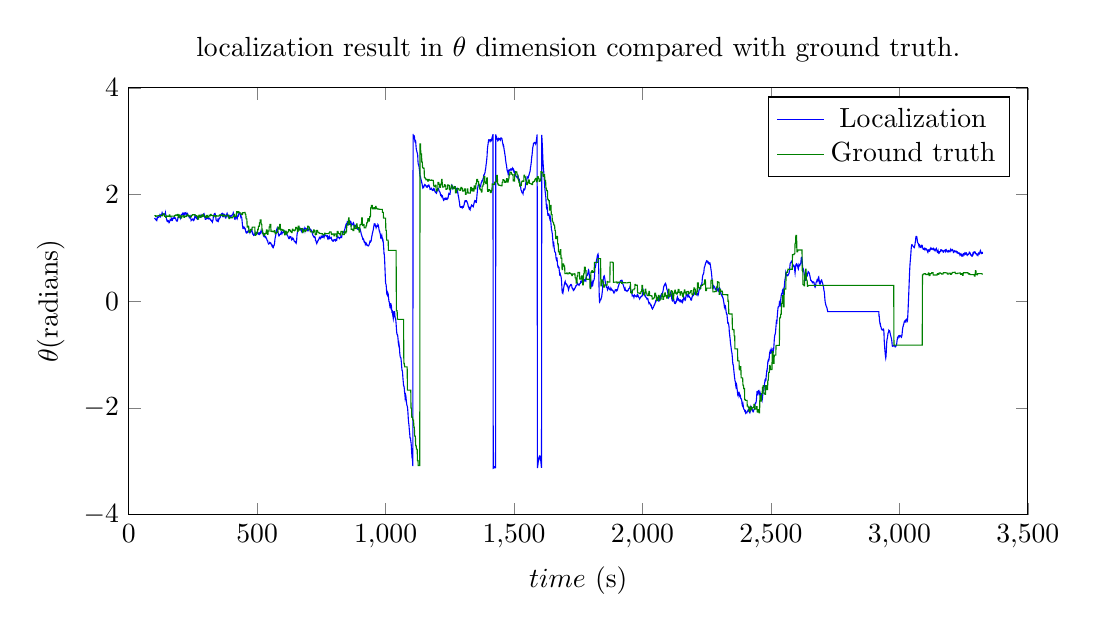
\begin{tikzpicture}

\begin{axis}[
title={localization result in $\theta$ dimension compared with ground truth.},
xlabel={$time$ (s)},
ylabel={$\theta$(radians)},
xmin=0, xmax=3500,
ymin=-4, ymax=4,
axis on top,
width=13cm,
height=7cm,
legend entries={{Localization},{Ground truth}}
]
\addplot [blue]
coordinates {
(100,1.54646635055542)
(101,1.5507230758667)
(102,1.55200612545013)
(103,1.54343175888062)
(104,1.54110467433929)
(105,1.52699089050293)
(106,1.52813470363617)
(107,1.52990198135376)
(108,1.52065563201904)
(109,1.53732943534851)
(110,1.52707743644714)
(111,1.55147683620453)
(112,1.56919050216675)
(113,1.57880342006683)
(114,1.57398235797882)
(115,1.57718074321747)
(116,1.57820665836334)
(117,1.57252848148346)
(118,1.58456563949585)
(119,1.58783566951752)
(120,1.60273432731628)
(121,1.61495399475098)
(122,1.59551870822906)
(123,1.59297847747803)
(124,1.58525991439819)
(125,1.61732733249664)
(126,1.61871790885925)
(127,1.62369799613953)
(128,1.62525105476379)
(129,1.64066576957703)
(130,1.65852236747742)
(131,1.6448974609375)
(132,1.62544429302216)
(133,1.62191128730774)
(134,1.62206280231476)
(135,1.6311856508255)
(136,1.62068057060242)
(137,1.62268495559692)
(138,1.62456870079041)
(139,1.623166680336)
(140,1.62601387500763)
(141,1.63756096363068)
(142,1.63515949249268)
(143,1.65911340713501)
(144,1.62978839874268)
(145,1.60041117668152)
(146,1.57306587696075)
(147,1.53875529766083)
(148,1.52924859523773)
(149,1.50976634025574)
(150,1.49467277526855)
(151,1.49296140670776)
(152,1.50407910346985)
(153,1.51181304454803)
(154,1.5095773935318)
(155,1.49384593963623)
(156,1.48523736000061)
(157,1.47079229354858)
(158,1.47306108474731)
(159,1.49335587024689)
(160,1.50466322898865)
(161,1.52211201190948)
(162,1.51193571090698)
(163,1.51525676250458)
(164,1.51930201053619)
(165,1.52878403663635)
(166,1.5528769493103)
(167,1.5430098772049)
(168,1.5275319814682)
(169,1.53846096992493)
(170,1.54615044593811)
(171,1.53192389011383)
(172,1.54811489582062)
(173,1.55466306209564)
(174,1.5524435043335)
(175,1.56175208091736)
(176,1.55368077754974)
(177,1.55463993549347)
(178,1.56228625774384)
(179,1.56938219070435)
(180,1.56852638721466)
(181,1.55836760997772)
(182,1.54815232753754)
(183,1.54338419437408)
(184,1.5323748588562)
(185,1.51234364509583)
(186,1.51337778568268)
(187,1.50604808330536)
(188,1.49984133243561)
(189,1.50034296512604)
(190,1.51631021499634)
(191,1.54578185081482)
(192,1.5680410861969)
(193,1.57312214374542)
(194,1.5728554725647)
(195,1.57949018478394)
(196,1.58402860164642)
(197,1.58160173892975)
(198,1.57810413837433)
(199,1.57278764247894)
(200,1.56922948360443)
(201,1.55482828617096)
(202,1.57609832286835)
(203,1.60039174556732)
(204,1.60224497318268)
(205,1.6195262670517)
(206,1.62399852275848)
(207,1.62016260623932)
(208,1.62961506843567)
(209,1.64186537265778)
(210,1.63222968578339)
(211,1.63029503822327)
(212,1.6494687795639)
(213,1.65180921554565)
(214,1.64489102363586)
(215,1.62831044197083)
(216,1.621626496315)
(217,1.64517664909363)
(218,1.64712762832642)
(219,1.66132891178131)
(220,1.66068875789642)
(221,1.6459082365036)
(222,1.63722383975983)
(223,1.62424039840698)
(224,1.61097288131714)
(225,1.61557412147522)
(226,1.62690734863281)
(227,1.65233135223389)
(228,1.64578688144684)
(229,1.64164483547211)
(230,1.62688159942627)
(231,1.61308217048645)
(232,1.60305392742157)
(233,1.59496462345123)
(234,1.59501135349274)
(235,1.58456933498383)
(236,1.56549787521362)
(237,1.57092916965485)
(238,1.59638440608978)
(239,1.60236072540283)
(240,1.58923435211182)
(241,1.56709229946136)
(242,1.54149341583252)
(243,1.51280212402344)
(244,1.52009916305542)
(245,1.5202465057373)
(246,1.52246618270874)
(247,1.52954256534576)
(248,1.53248751163483)
(249,1.5288952589035)
(250,1.54034495353699)
(251,1.53646886348724)
(252,1.52303040027618)
(253,1.53770112991333)
(254,1.54022860527039)
(255,1.53205502033234)
(256,1.54812002182007)
(257,1.57860517501831)
(258,1.60740625858307)
(259,1.61095333099365)
(260,1.59215152263641)
(261,1.57432639598846)
(262,1.5670051574707)
(263,1.5609986782074)
(264,1.5737726688385)
(265,1.56092166900635)
(266,1.54979717731476)
(267,1.53714156150818)
(268,1.53360104560852)
(269,1.53752386569977)
(270,1.55068731307983)
(271,1.55556619167328)
(272,1.57581460475922)
(273,1.58535003662109)
(274,1.58037567138672)
(275,1.5880218744278)
(276,1.59956812858582)
(277,1.59648048877716)
(278,1.58395183086395)
(279,1.58802652359009)
(280,1.58747506141663)
(281,1.60288035869598)
(282,1.58240473270416)
(283,1.59035933017731)
(284,1.60025298595428)
(285,1.60764396190643)
(286,1.59284281730652)
(287,1.59453332424164)
(288,1.59284269809723)
(289,1.59306907653809)
(290,1.59942615032196)
(291,1.6060471534729)
(292,1.63856315612793)
(293,1.64231729507446)
(294,1.62127292156219)
(295,1.58939063549042)
(296,1.57206177711487)
(297,1.56600487232208)
(298,1.53695380687714)
(299,1.5343781709671)
(300,1.53513896465302)
(301,1.54306077957153)
(302,1.54423141479492)
(303,1.54999113082886)
(304,1.56252479553223)
(305,1.56171059608459)
(306,1.56622409820557)
(307,1.56085908412933)
(308,1.563889503479)
(309,1.54371774196625)
(310,1.54420685768127)
(311,1.54266798496246)
(312,1.54999840259552)
(313,1.55634391307831)
(314,1.55178380012512)
(315,1.54730880260468)
(316,1.54921805858612)
(317,1.54176342487335)
(318,1.52773118019104)
(319,1.51913952827454)
(320,1.51811480522156)
(321,1.5204051733017)
(322,1.5196361541748)
(323,1.5025395154953)
(324,1.50740218162537)
(325,1.50768744945526)
(326,1.4912223815918)
(327,1.51467084884644)
(328,1.52037048339844)
(329,1.56555330753326)
(330,1.57597947120667)
(331,1.60047376155853)
(332,1.62293457984924)
(333,1.63446438312531)
(334,1.64028716087341)
(335,1.64710938930511)
(336,1.64744484424591)
(337,1.62508463859558)
(338,1.6042320728302)
(339,1.57648229598999)
(340,1.53094255924225)
(341,1.51199889183044)
(342,1.50783085823059)
(343,1.50807070732117)
(344,1.51170301437378)
(345,1.49789023399353)
(346,1.50170087814331)
(347,1.52624249458313)
(348,1.51726365089417)
(349,1.50466871261597)
(350,1.5200936794281)
(351,1.5475218296051)
(352,1.54299235343933)
(353,1.54903376102448)
(354,1.55820608139038)
(355,1.56096911430359)
(356,1.57267463207245)
(357,1.58465588092804)
(358,1.60979747772217)
(359,1.62278532981873)
(360,1.62996363639832)
(361,1.63382434844971)
(362,1.63811755180359)
(363,1.64475631713867)
(364,1.64732873439789)
(365,1.60888993740082)
(366,1.58858096599579)
(367,1.58332288265228)
(368,1.58434569835663)
(369,1.61654877662659)
(370,1.606480717659)
(371,1.62519037723541)
(372,1.62910878658295)
(373,1.62205302715302)
(374,1.6179986000061)
(375,1.59644711017609)
(376,1.56787407398224)
(377,1.56435573101044)
(378,1.5593169927597)
(379,1.56953537464142)
(380,1.5965723991394)
(381,1.62884426116943)
(382,1.63840901851654)
(383,1.64823424816132)
(384,1.6319864988327)
(385,1.61179351806641)
(386,1.59410321712494)
(387,1.58036863803864)
(388,1.57623171806335)
(389,1.58725047111511)
(390,1.5983966588974)
(391,1.57964026927948)
(392,1.5861576795578)
(393,1.59166240692139)
(394,1.59796917438507)
(395,1.58046758174896)
(396,1.57467401027679)
(397,1.58991885185242)
(398,1.58556258678436)
(399,1.5945326089859)
(400,1.6069518327713)
(401,1.60705900192261)
(402,1.60727155208588)
(403,1.61696755886078)
(404,1.61921179294586)
(405,1.63002061843872)
(406,1.64118611812592)
(407,1.65837097167969)
(408,1.64355742931366)
(409,1.61205804347992)
(410,1.59081983566284)
(411,1.57681131362915)
(412,1.5596159696579)
(413,1.53693175315857)
(414,1.5348140001297)
(415,1.5578316450119)
(416,1.57648587226868)
(417,1.57490694522858)
(418,1.57248783111572)
(419,1.56441628932953)
(420,1.55932223796844)
(421,1.55426454544067)
(422,1.54428219795227)
(423,1.5647851228714)
(424,1.58603322505951)
(425,1.60754644870758)
(426,1.61471712589264)
(427,1.60713183879852)
(428,1.63418853282928)
(429,1.64039397239685)
(430,1.65499937534332)
(431,1.65660297870636)
(432,1.6419951915741)
(433,1.63388311862946)
(434,1.62777280807495)
(435,1.61731600761414)
(436,1.58878862857819)
(437,1.60379076004028)
(438,1.581658244133)
(439,1.57688403129578)
(440,1.56658458709717)
(441,1.52402472496033)
(442,1.46749365329742)
(443,1.41576373577118)
(444,1.38739728927612)
(445,1.40081202983856)
(446,1.39354419708252)
(447,1.37017107009888)
(448,1.3655834197998)
(449,1.37958705425262)
(450,1.38273334503174)
(451,1.38543045520782)
(452,1.35608196258545)
(453,1.3548321723938)
(454,1.35424637794495)
(455,1.3186936378479)
(456,1.3022243976593)
(457,1.28345441818237)
(458,1.27933430671692)
(459,1.28356349468231)
(460,1.29277086257935)
(461,1.28453350067139)
(462,1.28917789459229)
(463,1.3112508058548)
(464,1.31334209442139)
(465,1.31213617324829)
(466,1.32059681415558)
(467,1.31306123733521)
(468,1.32198393344879)
(469,1.3208110332489)
(470,1.31313562393188)
(471,1.31415390968323)
(472,1.2836799621582)
(473,1.2930428981781)
(474,1.29822432994843)
(475,1.30777418613434)
(476,1.31536865234375)
(477,1.31040692329407)
(478,1.32143473625183)
(479,1.3376590013504)
(480,1.31458342075348)
(481,1.29817759990692)
(482,1.27101814746857)
(483,1.27618944644928)
(484,1.25679433345795)
(485,1.2522839307785)
(486,1.23904418945312)
(487,1.2454868555069)
(488,1.2496292591095)
(489,1.24159801006317)
(490,1.24774920940399)
(491,1.25974822044373)
(492,1.2701233625412)
(493,1.27594220638275)
(494,1.2712516784668)
(495,1.28047657012939)
(496,1.25796937942505)
(497,1.25784277915955)
(498,1.2649177312851)
(499,1.26540470123291)
(500,1.26543748378754)
(501,1.29331862926483)
(502,1.29143989086151)
(503,1.28305554389954)
(504,1.27083170413971)
(505,1.25791037082672)
(506,1.25478851795197)
(507,1.27684772014618)
(508,1.28055322170258)
(509,1.27176856994629)
(510,1.25923943519592)
(511,1.2687920331955)
(512,1.28335881233215)
(513,1.27762699127197)
(514,1.30205249786377)
(515,1.32051074504852)
(516,1.30292642116547)
(517,1.30597615242004)
(518,1.30810463428497)
(519,1.2921689748764)
(520,1.30164563655853)
(521,1.30991506576538)
(522,1.27794313430786)
(523,1.25076496601105)
(524,1.23437190055847)
(525,1.22034740447998)
(526,1.21851360797882)
(527,1.21013343334198)
(528,1.21249973773956)
(529,1.21446716785431)
(530,1.22987020015717)
(531,1.2035768032074)
(532,1.19230258464813)
(533,1.19355642795563)
(534,1.19935822486877)
(535,1.18313694000244)
(536,1.18168067932129)
(537,1.16821491718292)
(538,1.15258288383484)
(539,1.13940727710724)
(540,1.13065266609192)
(541,1.13280248641968)
(542,1.10339212417603)
(543,1.08896732330322)
(544,1.07642912864685)
(545,1.07113480567932)
(546,1.07907724380493)
(547,1.07880294322968)
(548,1.08189344406128)
(549,1.10488390922546)
(550,1.10379195213318)
(551,1.09952199459076)
(552,1.08417117595673)
(553,1.08199536800385)
(554,1.08405113220215)
(555,1.0606997013092)
(556,1.05767059326172)
(557,1.05229568481445)
(558,1.02904903888702)
(559,1.02926313877106)
(560,1.01883637905121)
(561,1.03455209732056)
(562,1.02246522903442)
(563,1.01281082630157)
(564,1.03416681289673)
(565,1.03952038288116)
(566,1.04426825046539)
(567,1.06625080108643)
(568,1.09912419319153)
(569,1.15294706821442)
(570,1.18021333217621)
(571,1.20422840118408)
(572,1.23102819919586)
(573,1.26146531105042)
(574,1.29849541187286)
(575,1.31607615947723)
(576,1.34390187263489)
(577,1.36058223247528)
(578,1.37074446678162)
(579,1.33955585956573)
(580,1.31531167030334)
(581,1.30118381977081)
(582,1.27478754520416)
(583,1.2477685213089)
(584,1.23455107212067)
(585,1.22328436374664)
(586,1.22746884822845)
(587,1.25170862674713)
(588,1.2514237165451)
(589,1.25478863716125)
(590,1.25799882411957)
(591,1.25375866889954)
(592,1.2595978975296)
(593,1.28568422794342)
(594,1.304607629776)
(595,1.3019026517868)
(596,1.29561722278595)
(597,1.27398836612701)
(598,1.29067754745483)
(599,1.29177844524384)
(600,1.29222273826599)
(601,1.2895233631134)
(602,1.29485750198364)
(603,1.30337047576904)
(604,1.28972280025482)
(605,1.29144597053528)
(606,1.30378270149231)
(607,1.27595794200897)
(608,1.26570892333984)
(609,1.26573348045349)
(610,1.27480757236481)
(611,1.27591192722321)
(612,1.28462815284729)
(613,1.27454102039337)
(614,1.27081680297852)
(615,1.2578296661377)
(616,1.26266169548035)
(617,1.23566567897797)
(618,1.22814154624939)
(619,1.22702872753143)
(620,1.21385586261749)
(621,1.20171189308167)
(622,1.1866307258606)
(623,1.18884932994843)
(624,1.17117965221405)
(625,1.17237818241119)
(626,1.18987798690796)
(627,1.20946168899536)
(628,1.20522797107697)
(629,1.20533299446106)
(630,1.21175622940063)
(631,1.21104490756989)
(632,1.18609893321991)
(633,1.16655659675598)
(634,1.15432524681091)
(635,1.16622424125671)
(636,1.1551228761673)
(637,1.15811955928802)
(638,1.16358411312103)
(639,1.18339478969574)
(640,1.17606866359711)
(641,1.17011070251465)
(642,1.16491544246674)
(643,1.14238727092743)
(644,1.13089883327484)
(645,1.11955177783966)
(646,1.11849558353424)
(647,1.12391364574432)
(648,1.12021267414093)
(649,1.09556782245636)
(650,1.09381246566772)
(651,1.09677803516388)
(652,1.08899211883545)
(653,1.12127554416656)
(654,1.15882349014282)
(655,1.23577475547791)
(656,1.27397441864014)
(657,1.29096794128418)
(658,1.31561732292175)
(659,1.34134304523468)
(660,1.35326290130615)
(661,1.35195338726044)
(662,1.36913073062897)
(663,1.37681412696838)
(664,1.37251007556915)
(665,1.36404073238373)
(666,1.36350500583649)
(667,1.3528960943222)
(668,1.3665109872818)
(669,1.36687994003296)
(670,1.36124551296234)
(671,1.35167551040649)
(672,1.31228959560394)
(673,1.31578397750854)
(674,1.3032740354538)
(675,1.33138334751129)
(676,1.32863461971283)
(677,1.36087965965271)
(678,1.36383414268494)
(679,1.35398101806641)
(680,1.34483051300049)
(681,1.34267330169678)
(682,1.34135580062866)
(683,1.33873748779297)
(684,1.3418402671814)
(685,1.36053097248077)
(686,1.32948291301727)
(687,1.36269843578339)
(688,1.36292505264282)
(689,1.36727643013)
(690,1.3658185005188)
(691,1.36178362369537)
(692,1.35471439361572)
(693,1.34621500968933)
(694,1.33173680305481)
(695,1.32545912265778)
(696,1.32827579975128)
(697,1.33804380893707)
(698,1.32484102249146)
(699,1.33909583091736)
(700,1.33238101005554)
(701,1.33680593967438)
(702,1.35841262340546)
(703,1.37371432781219)
(704,1.36128211021423)
(705,1.36123085021973)
(706,1.35309898853302)
(707,1.34598338603973)
(708,1.34184467792511)
(709,1.34034490585327)
(710,1.32120549678802)
(711,1.31259512901306)
(712,1.32333850860596)
(713,1.31777954101562)
(714,1.29025042057037)
(715,1.26415371894836)
(716,1.24970841407776)
(717,1.24008023738861)
(718,1.2268089056015)
(719,1.22140443325043)
(720,1.20806753635406)
(721,1.205002784729)
(722,1.19956791400909)
(723,1.20486485958099)
(724,1.20812571048737)
(725,1.20618391036987)
(726,1.18776309490204)
(727,1.14418888092041)
(728,1.14474976062775)
(729,1.12710583209991)
(730,1.11058914661407)
(731,1.09295690059662)
(732,1.0808128118515)
(733,1.0982369184494)
(734,1.11011445522308)
(735,1.10904312133789)
(736,1.12709522247314)
(737,1.14157497882843)
(738,1.14029252529144)
(739,1.15136468410492)
(740,1.16540157794952)
(741,1.17201101779938)
(742,1.19090437889099)
(743,1.18093073368073)
(744,1.18668186664581)
(745,1.17532193660736)
(746,1.16976523399353)
(747,1.17742264270782)
(748,1.19435751438141)
(749,1.21005427837372)
(750,1.19732511043549)
(751,1.20466613769531)
(752,1.21595120429993)
(753,1.21822392940521)
(754,1.20664668083191)
(755,1.21464967727661)
(756,1.20553290843964)
(757,1.22550904750824)
(758,1.21712005138397)
(759,1.22392988204956)
(760,1.23322546482086)
(761,1.20955157279968)
(762,1.23037242889404)
(763,1.22837555408478)
(764,1.23058187961578)
(765,1.23141849040985)
(766,1.23630774021149)
(767,1.22480809688568)
(768,1.22473478317261)
(769,1.22964799404144)
(770,1.22133266925812)
(771,1.21516263484955)
(772,1.22098422050476)
(773,1.22452211380005)
(774,1.18755269050598)
(775,1.20095896720886)
(776,1.21150064468384)
(777,1.20419633388519)
(778,1.1862051486969)
(779,1.1705002784729)
(780,1.17887461185455)
(781,1.2017787694931)
(782,1.17297184467316)
(783,1.17422139644623)
(784,1.18142020702362)
(785,1.18711638450623)
(786,1.18930435180664)
(787,1.1989403963089)
(788,1.20027792453766)
(789,1.18233168125153)
(790,1.16371762752533)
(791,1.14449393749237)
(792,1.1450172662735)
(793,1.14369451999664)
(794,1.13600516319275)
(795,1.1232453584671)
(796,1.12225413322449)
(797,1.14233672618866)
(798,1.14817273616791)
(799,1.14915299415588)
(800,1.15340113639832)
(801,1.1553807258606)
(802,1.15575325489044)
(803,1.13840007781982)
(804,1.14065635204315)
(805,1.13322949409485)
(806,1.14656591415405)
(807,1.13671445846558)
(808,1.14029324054718)
(809,1.15743601322174)
(810,1.15141713619232)
(811,1.17745411396027)
(812,1.19875013828278)
(813,1.19888424873352)
(814,1.21511828899384)
(815,1.19655275344849)
(816,1.19506931304932)
(817,1.19792103767395)
(818,1.19481670856476)
(819,1.18780171871185)
(820,1.17691707611084)
(821,1.18562340736389)
(822,1.19111132621765)
(823,1.19631397724152)
(824,1.1994194984436)
(825,1.19529592990875)
(826,1.21472823619843)
(827,1.2072674036026)
(828,1.19888687133789)
(829,1.19625222682953)
(830,1.23055708408356)
(831,1.26048624515533)
(832,1.2704176902771)
(833,1.27713215351105)
(834,1.29607903957367)
(835,1.29107475280762)
(836,1.28610098361969)
(837,1.28434646129608)
(838,1.30902850627899)
(839,1.31891441345215)
(840,1.317218542099)
(841,1.3475307226181)
(842,1.36206603050232)
(843,1.38236379623413)
(844,1.40265655517578)
(845,1.41999089717865)
(846,1.44056308269501)
(847,1.44905412197113)
(848,1.44622123241425)
(849,1.4569718837738)
(850,1.45706975460052)
(851,1.4935165643692)
(852,1.4900039434433)
(853,1.45230913162231)
(854,1.43999302387238)
(855,1.43049967288971)
(856,1.43197238445282)
(857,1.43750011920929)
(858,1.44223082065582)
(859,1.46671485900879)
(860,1.48139548301697)
(861,1.4770120382309)
(862,1.46721994876862)
(863,1.4814270734787)
(864,1.49399018287659)
(865,1.48691654205322)
(866,1.46614801883698)
(867,1.44620215892792)
(868,1.42293417453766)
(869,1.43342924118042)
(870,1.43596518039703)
(871,1.4438464641571)
(872,1.44296598434448)
(873,1.45508873462677)
(874,1.46581745147705)
(875,1.44759511947632)
(876,1.45657157897949)
(877,1.4422333240509)
(878,1.41276371479034)
(879,1.39574408531189)
(880,1.40863847732544)
(881,1.4055118560791)
(882,1.41721022129059)
(883,1.42020201683044)
(884,1.40497243404388)
(885,1.37675654888153)
(886,1.36979734897614)
(887,1.37533187866211)
(888,1.37540102005005)
(889,1.38342869281769)
(890,1.38675737380981)
(891,1.3597457408905)
(892,1.34746265411377)
(893,1.34471797943115)
(894,1.34996390342712)
(895,1.36478817462921)
(896,1.35776698589325)
(897,1.35930013656616)
(898,1.3421618938446)
(899,1.3440934419632)
(900,1.3428430557251)
(901,1.34826445579529)
(902,1.32716953754425)
(903,1.30974698066711)
(904,1.28942799568176)
(905,1.26747477054596)
(906,1.24680066108704)
(907,1.24066710472107)
(908,1.21116924285889)
(909,1.20690155029297)
(910,1.19162178039551)
(911,1.16798508167267)
(912,1.17248380184174)
(913,1.15935564041138)
(914,1.16310977935791)
(915,1.15011382102966)
(916,1.12016987800598)
(917,1.10739624500275)
(918,1.10351812839508)
(919,1.11175191402435)
(920,1.1004399061203)
(921,1.07188332080841)
(922,1.08816063404083)
(923,1.09245789051056)
(924,1.07944917678833)
(925,1.06686806678772)
(926,1.07517921924591)
(927,1.061394572258)
(928,1.05926036834717)
(929,1.04739427566528)
(930,1.04442918300629)
(931,1.04059767723083)
(932,1.03534412384033)
(933,1.03738677501678)
(934,1.04160237312317)
(935,1.0510790348053)
(936,1.06797659397125)
(937,1.07655131816864)
(938,1.09252095222473)
(939,1.12846660614014)
(940,1.12929260730743)
(941,1.12722146511078)
(942,1.11597442626953)
(943,1.12403297424316)
(944,1.13625931739807)
(945,1.17924857139587)
(946,1.20554327964783)
(947,1.22681760787964)
(948,1.25861585140228)
(949,1.28282880783081)
(950,1.2969411611557)
(951,1.31886970996857)
(952,1.33706998825073)
(953,1.37445676326752)
(954,1.3991607427597)
(955,1.42801856994629)
(956,1.45074224472046)
(957,1.44832372665405)
(958,1.43553376197815)
(959,1.44273269176483)
(960,1.42947781085968)
(961,1.40008354187012)
(962,1.39550292491913)
(963,1.37634766101837)
(964,1.38998484611511)
(965,1.40760922431946)
(966,1.39934587478638)
(967,1.40333521366119)
(968,1.40221512317657)
(969,1.40720546245575)
(970,1.43755781650543)
(971,1.4286847114563)
(972,1.41986191272736)
(973,1.38964378833771)
(974,1.35542976856232)
(975,1.32998931407928)
(976,1.30621540546417)
(977,1.30897986888885)
(978,1.27886736392975)
(979,1.26323127746582)
(980,1.24334800243378)
(981,1.18373882770538)
(982,1.18105828762054)
(983,1.21284294128418)
(984,1.2207053899765)
(985,1.23533046245575)
(986,1.20115399360657)
(987,1.1853883266449)
(988,1.15376222133636)
(989,1.13405108451843)
(990,1.14301788806915)
(991,1.10477674007416)
(992,1.04367291927338)
(993,0.968463599681854)
(994,0.884127497673035)
(995,0.879950165748596)
(996,0.798214972019196)
(997,0.687262177467346)
(998,0.563006222248077)
(999,0.452018111944199)
(1000,0.338105052709579)
(1001,0.32542210817337)
(1002,0.30710905790329)
(1003,0.254687160253525)
(1004,0.175329059362411)
(1005,0.127600938081741)
(1006,0.128926753997803)
(1007,0.11711497604847)
(1008,0.163483887910843)
(1009,0.152515083551407)
(1010,0.135648414492607)
(1011,0.0898915529251099)
(1012,0.0436864160001278)
(1013,-0.00425823777914047)
(1014,-0.0062735341489315)
(1015,-0.0400387793779373)
(1016,-0.0698819309473038)
(1017,-0.112447008490562)
(1018,-0.122866481542587)
(1019,-0.0903691500425339)
(1020,-0.0482197180390358)
(1021,-0.0527022741734982)
(1022,-0.0787253081798553)
(1023,-0.112014710903168)
(1024,-0.170169785618782)
(1025,-0.215001776814461)
(1026,-0.216772630810738)
(1027,-0.206613957881927)
(1028,-0.263907760381699)
(1029,-0.289958477020264)
(1030,-0.324967533349991)
(1031,-0.286519408226013)
(1032,-0.233948364853859)
(1033,-0.195228680968285)
(1034,-0.195180431008339)
(1035,-0.196672186255455)
(1036,-0.252596408128738)
(1037,-0.307751327753067)
(1038,-0.318871438503265)
(1039,-0.323613613843918)
(1040,-0.373806118965149)
(1041,-0.428775906562805)
(1042,-0.504394233226776)
(1043,-0.566873133182526)
(1044,-0.614800870418549)
(1045,-0.627846777439117)
(1046,-0.626067876815796)
(1047,-0.644636154174805)
(1048,-0.681740403175354)
(1049,-0.752928078174591)
(1050,-0.799487233161926)
(1051,-0.822168588638306)
(1052,-0.797708094120026)
(1053,-0.833521842956543)
(1054,-0.879625618457794)
(1055,-0.96374922990799)
(1056,-1.00997376441956)
(1057,-1.04395687580109)
(1058,-1.05350315570831)
(1059,-1.05407047271729)
(1060,-1.08105540275574)
(1061,-1.12534773349762)
(1062,-1.19599771499634)
(1063,-1.25097334384918)
(1064,-1.29706525802612)
(1065,-1.30162131786346)
(1066,-1.33239805698395)
(1067,-1.40852308273315)
(1068,-1.47295141220093)
(1069,-1.52217376232147)
(1070,-1.58608615398407)
(1071,-1.58823573589325)
(1072,-1.60609924793243)
(1073,-1.64489877223969)
(1074,-1.71365821361542)
(1075,-1.74567782878876)
(1076,-1.8055671453476)
(1077,-1.77476048469543)
(1078,-1.75578963756561)
(1079,-1.77788865566254)
(1080,-1.83007526397705)
(1081,-1.88177621364594)
(1082,-1.922238945961)
(1083,-1.95540499687195)
(1084,-1.96390056610107)
(1085,-1.98183262348175)
(1086,-2.02894449234009)
(1087,-2.08943700790405)
(1088,-2.17184209823608)
(1089,-2.24163508415222)
(1090,-2.28855609893799)
(1091,-2.32136058807373)
(1092,-2.39027285575867)
(1093,-2.43909025192261)
(1094,-2.4898796081543)
(1095,-2.55867695808411)
(1096,-2.57473826408386)
(1097,-2.57326245307922)
(1098,-2.61709475517273)
(1099,-2.65244555473328)
(1100,-2.69988012313843)
(1101,-2.78646397590637)
(1102,-2.8668384552002)
(1103,-2.93334174156189)
(1104,-2.94996094703674)
(1105,-3.00281310081482)
(1106,-3.09213924407959)
(1107,3.13867807388306)
(1108,3.08301067352295)
(1109,3.05500268936157)
(1110,3.06650757789612)
(1111,3.10095524787903)
(1112,3.09887099266052)
(1113,3.04348969459534)
(1114,3.00139617919922)
(1115,3.00786185264587)
(1116,3.01237607002258)
(1117,3.00366830825806)
(1118,2.93307638168335)
(1119,2.87231540679932)
(1120,2.83278703689575)
(1121,2.82493209838867)
(1122,2.79919242858887)
(1123,2.78468561172485)
(1124,2.76377630233765)
(1125,2.73824954032898)
(1126,2.62787818908691)
(1127,2.57622838020325)
(1128,2.55920338630676)
(1129,2.56220722198486)
(1130,2.5266637802124)
(1131,2.49155855178833)
(1132,2.44733715057373)
(1133,2.39534449577332)
(1134,2.35412335395813)
(1135,2.3311026096344)
(1136,2.33067274093628)
(1137,2.29847693443298)
(1138,2.27934336662292)
(1139,2.25910758972168)
(1140,2.24460053443909)
(1141,2.21784567832947)
(1142,2.19734859466553)
(1143,2.1706554889679)
(1144,2.14718079566956)
(1145,2.12594604492188)
(1146,2.13555097579956)
(1147,2.12668204307556)
(1148,2.12794876098633)
(1149,2.14651036262512)
(1150,2.17267608642578)
(1151,2.17536091804504)
(1152,2.18301391601562)
(1153,2.17237329483032)
(1154,2.17819285392761)
(1155,2.17945408821106)
(1156,2.16862344741821)
(1157,2.16796064376831)
(1158,2.14507460594177)
(1159,2.14045476913452)
(1160,2.1446840763092)
(1161,2.15045499801636)
(1162,2.15574669837952)
(1163,2.14520883560181)
(1164,2.15587544441223)
(1165,2.15931987762451)
(1166,2.17060661315918)
(1167,2.16447043418884)
(1168,2.15838313102722)
(1169,2.17064666748047)
(1170,2.15872931480408)
(1171,2.14480781555176)
(1172,2.12621378898621)
(1173,2.09810590744019)
(1174,2.10135126113892)
(1175,2.09881639480591)
(1176,2.10565876960754)
(1177,2.10505270957947)
(1178,2.11525297164917)
(1179,2.1060996055603)
(1180,2.09464192390442)
(1181,2.08396983146667)
(1182,2.0798077583313)
(1183,2.07544898986816)
(1184,2.07792258262634)
(1185,2.07750582695007)
(1186,2.10676884651184)
(1187,2.11498069763184)
(1188,2.1104953289032)
(1189,2.08973121643066)
(1190,2.09290790557861)
(1191,2.07184100151062)
(1192,2.059818983078)
(1193,2.04580426216125)
(1194,2.04303908348083)
(1195,2.03808736801147)
(1196,2.04543495178223)
(1197,2.03164100646973)
(1198,2.02480387687683)
(1199,2.03980541229248)
(1200,2.06394243240356)
(1201,2.06869721412659)
(1202,2.07636713981628)
(1203,2.10508322715759)
(1204,2.11174654960632)
(1205,2.11725568771362)
(1206,2.1137547492981)
(1207,2.10059285163879)
(1208,2.07635164260864)
(1209,2.05693459510803)
(1210,2.05375838279724)
(1211,2.04631400108337)
(1212,2.04316401481628)
(1213,2.01721143722534)
(1214,1.99024605751038)
(1215,1.99290347099304)
(1216,1.98818254470825)
(1217,1.96810376644135)
(1218,1.98157131671906)
(1219,1.96904873847961)
(1220,1.96715557575226)
(1221,1.97308731079102)
(1222,1.95799827575684)
(1223,1.93757021427155)
(1224,1.91812205314636)
(1225,1.90322029590607)
(1226,1.89055037498474)
(1227,1.89569997787476)
(1228,1.90953540802002)
(1229,1.92043650150299)
(1230,1.92631852626801)
(1231,1.92121374607086)
(1232,1.92943060398102)
(1233,1.92062759399414)
(1234,1.90762662887573)
(1235,1.90554690361023)
(1236,1.90883409976959)
(1237,1.92707014083862)
(1238,1.92332851886749)
(1239,1.92782366275787)
(1240,1.91508841514587)
(1241,1.9231903553009)
(1242,1.92555963993073)
(1243,1.9350905418396)
(1244,1.9627673625946)
(1245,1.9993280172348)
(1246,2.01650047302246)
(1247,2.00923728942871)
(1248,2.00929999351501)
(1249,2.00458288192749)
(1250,2.01457381248474)
(1251,2.0115270614624)
(1252,2.06012940406799)
(1253,2.08697938919067)
(1254,2.11572623252869)
(1255,2.12685441970825)
(1256,2.14140224456787)
(1257,2.15828967094421)
(1258,2.17858791351318)
(1259,2.17227220535278)
(1260,2.13885974884033)
(1261,2.11816096305847)
(1262,2.12981867790222)
(1263,2.12251377105713)
(1264,2.12377643585205)
(1265,2.13475179672241)
(1266,2.14137673377991)
(1267,2.1323778629303)
(1268,2.13553285598755)
(1269,2.14897894859314)
(1270,2.14794540405273)
(1271,2.13769960403442)
(1272,2.12558674812317)
(1273,2.10545778274536)
(1274,2.10663676261902)
(1275,2.10731315612793)
(1276,2.08501577377319)
(1277,2.08365988731384)
(1278,2.10008144378662)
(1279,2.07093453407288)
(1280,2.06703162193298)
(1281,2.03041791915894)
(1282,2.00886273384094)
(1283,1.97411847114563)
(1284,1.95795738697052)
(1285,1.92945694923401)
(1286,1.89379048347473)
(1287,1.86369729042053)
(1288,1.83653318881989)
(1289,1.78872430324554)
(1290,1.76531445980072)
(1291,1.76233661174774)
(1292,1.75973224639893)
(1293,1.76181185245514)
(1294,1.77264392375946)
(1295,1.77149343490601)
(1296,1.76149797439575)
(1297,1.75566017627716)
(1298,1.74876379966736)
(1299,1.76264083385468)
(1300,1.77658665180206)
(1301,1.77348053455353)
(1302,1.75955581665039)
(1303,1.76250338554382)
(1304,1.78319323062897)
(1305,1.8000830411911)
(1306,1.81091320514679)
(1307,1.85195422172546)
(1308,1.85674488544464)
(1309,1.88216984272003)
(1310,1.88348627090454)
(1311,1.87821221351624)
(1312,1.87294793128967)
(1313,1.88389825820923)
(1314,1.88227796554565)
(1315,1.88268077373505)
(1316,1.86786353588104)
(1317,1.86620092391968)
(1318,1.84760475158691)
(1319,1.83529877662659)
(1320,1.82097709178925)
(1321,1.79746842384338)
(1322,1.77373766899109)
(1323,1.7738893032074)
(1324,1.75335299968719)
(1325,1.7394198179245)
(1326,1.75196814537048)
(1327,1.75430560112)
(1328,1.72284352779388)
(1329,1.71440052986145)
(1330,1.74536120891571)
(1331,1.74319851398468)
(1332,1.76511883735657)
(1333,1.78001344203949)
(1334,1.78837537765503)
(1335,1.80478274822235)
(1336,1.8016015291214)
(1337,1.784876704216)
(1338,1.7846086025238)
(1339,1.78748965263367)
(1340,1.77879047393799)
(1341,1.7713418006897)
(1342,1.78992557525635)
(1343,1.80702173709869)
(1344,1.82700395584106)
(1345,1.85231232643127)
(1346,1.86905527114868)
(1347,1.87859618663788)
(1348,1.86757481098175)
(1349,1.86684489250183)
(1350,1.8800345659256)
(1351,1.87438988685608)
(1352,1.85234928131104)
(1353,1.85188126564026)
(1354,1.89182090759277)
(1355,1.94338166713715)
(1356,1.99956464767456)
(1357,2.04684710502625)
(1358,2.11390018463135)
(1359,2.13407182693481)
(1360,2.17029356956482)
(1361,2.1816565990448)
(1362,2.19609236717224)
(1363,2.18815279006958)
(1364,2.16857028007507)
(1365,2.16333198547363)
(1366,2.15714001655579)
(1367,2.15056967735291)
(1368,2.14299511909485)
(1369,2.15087747573853)
(1370,2.16711235046387)
(1371,2.18857836723328)
(1372,2.21423983573914)
(1373,2.22498941421509)
(1374,2.22641324996948)
(1375,2.25927352905273)
(1376,2.26325011253357)
(1377,2.25897002220154)
(1378,2.26673722267151)
(1379,2.29289412498474)
(1380,2.29648232460022)
(1381,2.3215343952179)
(1382,2.36092257499695)
(1383,2.36946797370911)
(1384,2.36858654022217)
(1385,2.38013529777527)
(1386,2.40316772460938)
(1387,2.40856432914734)
(1388,2.4502227306366)
(1389,2.47224044799805)
(1390,2.49821400642395)
(1391,2.5548460483551)
(1392,2.5782208442688)
(1393,2.62320518493652)
(1394,2.67367720603943)
(1395,2.72409391403198)
(1396,2.82087111473083)
(1397,2.88023853302002)
(1398,2.91866493225098)
(1399,2.94853973388672)
(1400,2.99102473258972)
(1401,3.02209448814392)
(1402,3.01845765113831)
(1403,3.01430130004883)
(1404,3.02421450614929)
(1405,3.02603578567505)
(1406,3.01350045204163)
(1407,2.99671363830566)
(1408,3.00670194625854)
(1409,3.01485824584961)
(1410,3.02972292900085)
(1411,3.03320503234863)
(1412,3.01818943023682)
(1413,3.03026056289673)
(1414,3.06016635894775)
(1415,3.07814121246338)
(1416,3.09030413627625)
(1417,3.10324311256409)
(1418,3.13132929801941)
(1419,-3.13228297233582)
(1420,-3.12915849685669)
(1421,-3.10962605476379)
(1422,-3.11107659339905)
(1423,-3.10755920410156)
(1424,-3.11238241195679)
(1425,-3.11813449859619)
(1426,-3.10296702384949)
(1427,-3.10020279884338)
(1428,-3.13137698173523)
(1429,3.12796258926392)
(1430,3.09330296516418)
(1431,3.08884596824646)
(1432,3.08422708511353)
(1433,3.042644739151)
(1434,3.03699684143066)
(1435,3.03901982307434)
(1436,3.03058242797852)
(1437,3.00936412811279)
(1438,3.01737499237061)
(1439,3.05412077903748)
(1440,3.0559675693512)
(1441,3.03874850273132)
(1442,3.02810978889465)
(1443,3.03271889686584)
(1444,3.04760956764221)
(1445,3.04876899719238)
(1446,3.04298305511475)
(1447,3.02920985221863)
(1448,3.0496711730957)
(1449,3.06114339828491)
(1450,3.05913043022156)
(1451,3.04937171936035)
(1452,3.05395436286926)
(1453,3.04639649391174)
(1454,3.01732492446899)
(1455,2.98322820663452)
(1456,2.96674394607544)
(1457,2.93055129051208)
(1458,2.91188430786133)
(1459,2.92157983779907)
(1460,2.90164875984192)
(1461,2.85631084442139)
(1462,2.82911992073059)
(1463,2.80613350868225)
(1464,2.76569437980652)
(1465,2.73713040351868)
(1466,2.7031078338623)
(1467,2.65409779548645)
(1468,2.62116122245789)
(1469,2.58248805999756)
(1470,2.56438755989075)
(1471,2.53212285041809)
(1472,2.49245095252991)
(1473,2.4625256061554)
(1474,2.44184637069702)
(1475,2.42240428924561)
(1476,2.41832685470581)
(1477,2.38882565498352)
(1478,2.4268114566803)
(1479,2.4059624671936)
(1480,2.42608380317688)
(1481,2.44260883331299)
(1482,2.44710779190063)
(1483,2.46473002433777)
(1484,2.46668004989624)
(1485,2.4654712677002)
(1486,2.46193099021912)
(1487,2.47558975219727)
(1488,2.48331189155579)
(1489,2.47922801971436)
(1490,2.46659302711487)
(1491,2.4567973613739)
(1492,2.45791721343994)
(1493,2.4663200378418)
(1494,2.49116230010986)
(1495,2.48228597640991)
(1496,2.47529006004333)
(1497,2.48027276992798)
(1498,2.4669942855835)
(1499,2.43873739242554)
(1500,2.44749283790588)
(1501,2.43372416496277)
(1502,2.43299531936646)
(1503,2.39912629127502)
(1504,2.37210774421692)
(1505,2.37429857254028)
(1506,2.37340903282166)
(1507,2.34512996673584)
(1508,2.34495377540588)
(1509,2.33835601806641)
(1510,2.33207154273987)
(1511,2.32300043106079)
(1512,2.317054271698)
(1513,2.32743954658508)
(1514,2.31814050674438)
(1515,2.32955002784729)
(1516,2.33652687072754)
(1517,2.31106686592102)
(1518,2.29593777656555)
(1519,2.27583956718445)
(1520,2.26027798652649)
(1521,2.2676956653595)
(1522,2.23523759841919)
(1523,2.21457862854004)
(1524,2.18818259239197)
(1525,2.17085742950439)
(1526,2.13162469863892)
(1527,2.08921241760254)
(1528,2.07937598228455)
(1529,2.07248711585999)
(1530,2.05234384536743)
(1531,2.03609871864319)
(1532,2.03902506828308)
(1533,2.03824329376221)
(1534,2.02903962135315)
(1535,2.01565337181091)
(1536,2.0474898815155)
(1537,2.07860779762268)
(1538,2.10478353500366)
(1539,2.10309076309204)
(1540,2.09147572517395)
(1541,2.10115671157837)
(1542,2.09819769859314)
(1543,2.11088752746582)
(1544,2.1530613899231)
(1545,2.19570446014404)
(1546,2.22030067443848)
(1547,2.24981164932251)
(1548,2.2399480342865)
(1549,2.25648641586304)
(1550,2.28438258171082)
(1551,2.33174705505371)
(1552,2.32758688926697)
(1553,2.32250094413757)
(1554,2.31776523590088)
(1555,2.313396692276)
(1556,2.32728338241577)
(1557,2.35490989685059)
(1558,2.36160731315613)
(1559,2.37969565391541)
(1560,2.39734292030334)
(1561,2.41527938842773)
(1562,2.42750430107117)
(1563,2.45617127418518)
(1564,2.50952386856079)
(1565,2.52729916572571)
(1566,2.56357574462891)
(1567,2.60137701034546)
(1568,2.65050554275513)
(1569,2.70970392227173)
(1570,2.7342369556427)
(1571,2.7831814289093)
(1572,2.84006714820862)
(1573,2.88059091567993)
(1574,2.90173435211182)
(1575,2.9307017326355)
(1576,2.96398138999939)
(1577,2.96518850326538)
(1578,2.958251953125)
(1579,2.96530604362488)
(1580,2.97605586051941)
(1581,2.97475671768188)
(1582,2.97412776947021)
(1583,2.97379493713379)
(1584,2.95448040962219)
(1585,2.9714207649231)
(1586,2.98457813262939)
(1587,3.02463293075562)
(1588,3.05568146705627)
(1589,3.08913469314575)
(1590,3.12644195556641)
(1591,-3.13021779060364)
(1592,-3.097825050354)
(1593,-3.065025806427)
(1594,-3.02140712738037)
(1595,-2.99506211280823)
(1596,-2.94693088531494)
(1597,-2.93356418609619)
(1598,-2.91785049438477)
(1599,-2.93618392944336)
(1600,-2.91419267654419)
(1601,-2.90685844421387)
(1602,-2.91171407699585)
(1603,-2.91894483566284)
(1604,-2.98590278625488)
(1605,-3.03811955451965)
(1606,-3.08911108970642)
(1607,-3.12604379653931)
(1608,3.11993312835693)
(1609,3.0214421749115)
(1610,2.9324164390564)
(1611,2.83168506622314)
(1612,2.69628500938416)
(1613,2.59661769866943)
(1614,2.52222609519958)
(1615,2.46840405464172)
(1616,2.40694499015808)
(1617,2.3368444442749)
(1618,2.25731897354126)
(1619,2.1786322593689)
(1620,2.10971832275391)
(1621,2.07043647766113)
(1622,2.02247452735901)
(1623,1.98472154140472)
(1624,1.93228709697723)
(1625,1.83847975730896)
(1626,1.78219425678253)
(1627,1.80517327785492)
(1628,1.80800783634186)
(1629,1.76682841777802)
(1630,1.70679152011871)
(1631,1.64223825931549)
(1632,1.6092791557312)
(1633,1.60847437381744)
(1634,1.62669384479523)
(1635,1.63715696334839)
(1636,1.63513541221619)
(1637,1.6047637462616)
(1638,1.56970858573914)
(1639,1.54749262332916)
(1640,1.56682503223419)
(1641,1.57935464382172)
(1642,1.54131186008453)
(1643,1.4944349527359)
(1644,1.44264936447144)
(1645,1.38502144813538)
(1646,1.33502805233002)
(1647,1.32586658000946)
(1648,1.28985714912415)
(1649,1.26703155040741)
(1650,1.20469057559967)
(1651,1.14103507995605)
(1652,1.07962334156036)
(1653,1.10953545570374)
(1654,1.11023342609406)
(1655,1.07201278209686)
(1656,1.01340222358704)
(1657,0.973615527153015)
(1658,0.940211117267609)
(1659,0.920096397399902)
(1660,0.91574239730835)
(1661,0.913928925991058)
(1662,0.898123443126678)
(1663,0.833438217639923)
(1664,0.791800558567047)
(1665,0.778915762901306)
(1666,0.802094757556915)
(1667,0.806292057037354)
(1668,0.766555488109589)
(1669,0.699564337730408)
(1670,0.668809711933136)
(1671,0.63965117931366)
(1672,0.631684303283691)
(1673,0.626856505870819)
(1674,0.641461372375488)
(1675,0.633486092090607)
(1676,0.578808784484863)
(1677,0.541830718517303)
(1678,0.492082893848419)
(1679,0.495317399501801)
(1680,0.507909297943115)
(1681,0.486890286207199)
(1682,0.477307826280594)
(1683,0.459152728319168)
(1684,0.429533332586288)
(1685,0.368689954280853)
(1686,0.289034694433212)
(1687,0.188745304942131)
(1688,0.157429829239845)
(1689,0.156482249498367)
(1690,0.148052364587784)
(1691,0.177926033735275)
(1692,0.202153533697128)
(1693,0.238253593444824)
(1694,0.262922465801239)
(1695,0.294275373220444)
(1696,0.316177874803543)
(1697,0.333701431751251)
(1698,0.359778583049774)
(1699,0.370046705007553)
(1700,0.336174041032791)
(1701,0.326084494590759)
(1702,0.332437515258789)
(1703,0.325723469257355)
(1704,0.325841844081879)
(1705,0.316147536039352)
(1706,0.293599188327789)
(1707,0.278347045183182)
(1708,0.278715193271637)
(1709,0.285421907901764)
(1710,0.258576542139053)
(1711,0.233653008937836)
(1712,0.212397903203964)
(1713,0.228423327207565)
(1714,0.246119394898415)
(1715,0.265827894210815)
(1716,0.275857180356979)
(1717,0.283015668392181)
(1718,0.290887087583542)
(1719,0.291893780231476)
(1720,0.310754537582397)
(1721,0.310668259859085)
(1722,0.31433442234993)
(1723,0.308861076831818)
(1724,0.296107709407806)
(1725,0.280688941478729)
(1726,0.245037436485291)
(1727,0.243356123566628)
(1728,0.233814015984535)
(1729,0.226240456104279)
(1730,0.225199654698372)
(1731,0.201852560043335)
(1732,0.206774219870567)
(1733,0.219693928956985)
(1734,0.230624869465828)
(1735,0.223910272121429)
(1736,0.234219238162041)
(1737,0.240692317485809)
(1738,0.24943183362484)
(1739,0.26695916056633)
(1740,0.267389595508575)
(1741,0.291087836027145)
(1742,0.291226774454117)
(1743,0.291542947292328)
(1744,0.298930823802948)
(1745,0.308268010616302)
(1746,0.310650795698166)
(1747,0.334159016609192)
(1748,0.326438516378403)
(1749,0.32094818353653)
(1750,0.313239753246307)
(1751,0.310497790575027)
(1752,0.304458022117615)
(1753,0.297567754983902)
(1754,0.305858135223389)
(1755,0.32523974776268)
(1756,0.326770335435867)
(1757,0.330034554004669)
(1758,0.331786662340164)
(1759,0.350412756204605)
(1760,0.376827150583267)
(1761,0.375532001256943)
(1762,0.363882809877396)
(1763,0.368616074323654)
(1764,0.37714546918869)
(1765,0.356053382158279)
(1766,0.359279900789261)
(1767,0.370634853839874)
(1768,0.367184668779373)
(1769,0.347810864448547)
(1770,0.358719944953918)
(1771,0.392676949501038)
(1772,0.381230711936951)
(1773,0.380191802978516)
(1774,0.380006939172745)
(1775,0.40419140458107)
(1776,0.404286921024323)
(1777,0.382669299840927)
(1778,0.389078080654144)
(1779,0.411669939756393)
(1780,0.397983103990555)
(1781,0.434322595596313)
(1782,0.467418342828751)
(1783,0.482483178377151)
(1784,0.491503655910492)
(1785,0.485195696353912)
(1786,0.489699572324753)
(1787,0.51929759979248)
(1788,0.534083306789398)
(1789,0.56996488571167)
(1790,0.587395250797272)
(1791,0.57914537191391)
(1792,0.536709070205688)
(1793,0.49285951256752)
(1794,0.446550190448761)
(1795,0.455974191427231)
(1796,0.42074117064476)
(1797,0.382558226585388)
(1798,0.336970865726471)
(1799,0.300708264112473)
(1800,0.276678860187531)
(1801,0.294614285230637)
(1802,0.334356874227524)
(1803,0.355166912078857)
(1804,0.31011238694191)
(1805,0.287834376096725)
(1806,0.292181223630905)
(1807,0.327368348836899)
(1808,0.352983981370926)
(1809,0.384807258844376)
(1810,0.3852459192276)
(1811,0.396453112363815)
(1812,0.410765200853348)
(1813,0.455575823783875)
(1814,0.537773251533508)
(1815,0.64652419090271)
(1816,0.659725427627563)
(1817,0.650731325149536)
(1818,0.672273397445679)
(1819,0.707446336746216)
(1820,0.735996842384338)
(1821,0.770284056663513)
(1822,0.788775980472565)
(1823,0.809050321578979)
(1824,0.844402611255646)
(1825,0.859178841114044)
(1826,0.876093149185181)
(1827,0.884447872638702)
(1828,0.849115252494812)
(1829,0.73991858959198)
(1830,0.509904623031616)
(1831,0.245248779654503)
(1832,0.058653686195612)
(1833,-0.0189470630139112)
(1834,-0.0127075063064694)
(1835,0.0167704671621323)
(1836,0.0300639290362597)
(1837,0.0244585182517767)
(1838,0.0287072751671076)
(1839,0.0453543290495872)
(1840,0.066745862364769)
(1841,0.0792692676186562)
(1842,0.11721608042717)
(1843,0.15308253467083)
(1844,0.196250185370445)
(1845,0.258979558944702)
(1846,0.329999297857285)
(1847,0.388670563697815)
(1848,0.420038193464279)
(1849,0.46053683757782)
(1850,0.468215346336365)
(1851,0.475532412528992)
(1852,0.459795206785202)
(1853,0.433088749647141)
(1854,0.398980885744095)
(1855,0.367423444986343)
(1856,0.34119525551796)
(1857,0.321995824575424)
(1858,0.305680930614471)
(1859,0.277709066867828)
(1860,0.286984324455261)
(1861,0.273436903953552)
(1862,0.254949629306793)
(1863,0.24085396528244)
(1864,0.212871178984642)
(1865,0.221915140748024)
(1866,0.238596349954605)
(1867,0.259406983852386)
(1868,0.267515778541565)
(1869,0.255177140235901)
(1870,0.239381656050682)
(1871,0.234269976615906)
(1872,0.22087299823761)
(1873,0.226244807243347)
(1874,0.226308271288872)
(1875,0.230165675282478)
(1876,0.219483762979507)
(1877,0.244779959321022)
(1878,0.233624815940857)
(1879,0.216670528054237)
(1880,0.221838757395744)
(1881,0.214648678898811)
(1882,0.206412881612778)
(1883,0.200509741902351)
(1884,0.205198764801025)
(1885,0.200916185975075)
(1886,0.193186417222023)
(1887,0.170020997524261)
(1888,0.157346531748772)
(1889,0.152422845363617)
(1890,0.171991348266602)
(1891,0.173593953251839)
(1892,0.173446804285049)
(1893,0.196394562721252)
(1894,0.211891695857048)
(1895,0.207554221153259)
(1896,0.209912180900574)
(1897,0.213572442531586)
(1898,0.203676149249077)
(1899,0.215363711118698)
(1900,0.214324861764908)
(1901,0.199822410941124)
(1902,0.207097709178925)
(1903,0.22564172744751)
(1904,0.235553935170174)
(1905,0.262141287326813)
(1906,0.282801747322083)
(1907,0.292033195495605)
(1908,0.309458047151566)
(1909,0.3264000415802)
(1910,0.328557699918747)
(1911,0.342311263084412)
(1912,0.359098225831985)
(1913,0.367455929517746)
(1914,0.378822535276413)
(1915,0.385996311903)
(1916,0.387476742267609)
(1917,0.383196294307709)
(1918,0.388982623815536)
(1919,0.394037365913391)
(1920,0.394193112850189)
(1921,0.37909922003746)
(1922,0.366690427064896)
(1923,0.351328343153)
(1924,0.312325835227966)
(1925,0.308625102043152)
(1926,0.294160932302475)
(1927,0.275963515043259)
(1928,0.24968945980072)
(1929,0.247012510895729)
(1930,0.227521017193794)
(1931,0.241994693875313)
(1932,0.248301401734352)
(1933,0.22203803062439)
(1934,0.203327268362045)
(1935,0.196079358458519)
(1936,0.195266589522362)
(1937,0.195645615458488)
(1938,0.198973968625069)
(1939,0.189478144049644)
(1940,0.184442296624184)
(1941,0.193050414323807)
(1942,0.198512181639671)
(1943,0.205297142267227)
(1944,0.203309789299965)
(1945,0.212876319885254)
(1946,0.225743353366852)
(1947,0.235615581274033)
(1948,0.237509816884995)
(1949,0.238636672496796)
(1950,0.242313370108604)
(1951,0.269601583480835)
(1952,0.262568086385727)
(1953,0.239772573113441)
(1954,0.221635699272156)
(1955,0.199849635362625)
(1956,0.185119286179543)
(1957,0.175579503178596)
(1958,0.164934635162354)
(1959,0.137943476438522)
(1960,0.103304475545883)
(1961,0.108663111925125)
(1962,0.111316002905369)
(1963,0.10713904350996)
(1964,0.0973565131425858)
(1965,0.107665918767452)
(1966,0.106279596686363)
(1967,0.0787907317280769)
(1968,0.0981286838650703)
(1969,0.112618923187256)
(1970,0.106118865311146)
(1971,0.102515168488026)
(1972,0.0982378348708153)
(1973,0.0973270088434219)
(1974,0.0904115289449692)
(1975,0.0904716476798058)
(1976,0.0810512080788612)
(1977,0.0822464749217033)
(1978,0.100345760583878)
(1979,0.0959202870726585)
(1980,0.12453056126833)
(1981,0.127945110201836)
(1982,0.0986494198441505)
(1983,0.0909735411405563)
(1984,0.0932078883051872)
(1985,0.0825120508670807)
(1986,0.0693941563367844)
(1987,0.0598501414060593)
(1988,0.0552134588360786)
(1989,0.0443760231137276)
(1990,0.0617103949189186)
(1991,0.0615556985139847)
(1992,0.0628563910722733)
(1993,0.0783596038818359)
(1994,0.0839481875300407)
(1995,0.0892328992486)
(1996,0.088930256664753)
(1997,0.097422756254673)
(1998,0.0953332409262657)
(1999,0.0974722802639008)
(2000,0.13289001584053)
(2001,0.158975630998611)
(2002,0.186979085206985)
(2003,0.202412843704224)
(2004,0.180154144763947)
(2005,0.156836792826653)
(2006,0.14875340461731)
(2007,0.13572658598423)
(2008,0.116544991731644)
(2009,0.106062524020672)
(2010,0.117914952337742)
(2011,0.0934873670339584)
(2012,0.0797193869948387)
(2013,0.0782283544540405)
(2014,0.066931277513504)
(2015,0.0636588037014008)
(2016,0.063140943646431)
(2017,0.0446330644190311)
(2018,0.0497329197824001)
(2019,0.0506106354296207)
(2020,0.0511963367462158)
(2021,0.0484718568623066)
(2022,0.0121493060141802)
(2023,0.00235207751393318)
(2024,-0.00977259874343872)
(2025,-0.0399415455758572)
(2026,-0.0348657518625259)
(2027,-0.0346590578556061)
(2028,-0.0313655734062195)
(2029,-0.0397004373371601)
(2030,-0.0613357312977314)
(2031,-0.063651368021965)
(2032,-0.0761081874370575)
(2033,-0.0693175345659256)
(2034,-0.0779335051774979)
(2035,-0.0926314368844032)
(2036,-0.119743548333645)
(2037,-0.13529098033905)
(2038,-0.137064412236214)
(2039,-0.144726201891899)
(2040,-0.132632806897163)
(2041,-0.123310431838036)
(2042,-0.118649251759052)
(2043,-0.106973566114902)
(2044,-0.10017441213131)
(2045,-0.0770881474018097)
(2046,-0.0756313726305962)
(2047,-0.0558169335126877)
(2048,-0.0569488331675529)
(2049,-0.041986495256424)
(2050,-0.0193721577525139)
(2051,-0.00263728527352214)
(2052,-0.00875202100723982)
(2053,0.000579149229452014)
(2054,0.0315046012401581)
(2055,0.0361400358378887)
(2056,0.0446089431643486)
(2057,0.0615237690508366)
(2058,0.063087172806263)
(2059,0.0612352974712849)
(2060,0.0501051731407642)
(2061,0.0671004131436348)
(2062,0.038099143654108)
(2063,0.00773697253316641)
(2064,8.69365758262575e-05)
(2065,0.00526466360315681)
(2066,0.0292632430791855)
(2067,0.0397790372371674)
(2068,0.0580431148409843)
(2069,0.0821994692087173)
(2070,0.094129353761673)
(2071,0.103481762111187)
(2072,0.0796875283122063)
(2073,0.114398553967476)
(2074,0.135561570525169)
(2075,0.137877434492111)
(2076,0.144563674926758)
(2077,0.146295174956322)
(2078,0.15729121863842)
(2079,0.172387644648552)
(2080,0.191684484481812)
(2081,0.215756759047508)
(2082,0.252905368804932)
(2083,0.2764031291008)
(2084,0.279337346553802)
(2085,0.29959100484848)
(2086,0.305999398231506)
(2087,0.322034418582916)
(2088,0.321804314851761)
(2089,0.313935399055481)
(2090,0.328612804412842)
(2091,0.316476613283157)
(2092,0.303023427724838)
(2093,0.267584443092346)
(2094,0.249758794903755)
(2095,0.220158979296684)
(2096,0.212880834937096)
(2097,0.203468233346939)
(2098,0.1734689027071)
(2099,0.144161909818649)
(2100,0.113355711102486)
(2101,0.0831395536661148)
(2102,0.0647189393639565)
(2103,0.0738934576511383)
(2104,0.0945555493235588)
(2105,0.113752245903015)
(2106,0.107729732990265)
(2107,0.118897475302219)
(2108,0.141520470380783)
(2109,0.156833648681641)
(2110,0.141930729150772)
(2111,0.141742140054703)
(2112,0.123927511274815)
(2113,0.0896462127566338)
(2114,0.0455613881349564)
(2115,0.0251939427107573)
(2116,0.00896425265818834)
(2117,0.00500478455796838)
(2118,0.0204825438559055)
(2119,0.0167282540351152)
(2120,0.0267848391085863)
(2121,0.0187409557402134)
(2122,0.0251833591610193)
(2123,-0.00251351576298475)
(2124,-0.0219194889068604)
(2125,-0.0329120680689812)
(2126,-0.0253466907888651)
(2127,-0.0391810350120068)
(2128,-0.0428864173591137)
(2129,-0.036336787045002)
(2130,-0.0149590559303761)
(2131,-0.0154695501551032)
(2132,0.00483938865363598)
(2133,0.0161772277206182)
(2134,0.0408340133726597)
(2135,0.0657291933894157)
(2136,0.0791917890310287)
(2137,0.0583108961582184)
(2138,0.0320769585669041)
(2139,0.0418966449797153)
(2140,0.0447067320346832)
(2141,0.0302121192216873)
(2142,0.0152673460543156)
(2143,0.0203928984701633)
(2144,0.00812397617846727)
(2145,0.0216567032039165)
(2146,0.0229427721351385)
(2147,0.0161252655088902)
(2148,0.00245388690382242)
(2149,0.0163261462002993)
(2150,0.00870827492326498)
(2151,-0.00333362584933639)
(2152,-0.00816372130066156)
(2153,-0.0151221146807075)
(2154,-0.000953582930378616)
(2155,-0.0157020222395658)
(2156,0.00599537650123239)
(2157,-0.00425323331728578)
(2158,0.0119557259604335)
(2159,0.0378049090504646)
(2160,0.0611865520477295)
(2161,0.0758091807365417)
(2162,0.0648518577218056)
(2163,0.0535648167133331)
(2164,0.0471685603260994)
(2165,0.0254629720002413)
(2166,0.0156011302024126)
(2167,0.0226710718125105)
(2168,0.0420004017651081)
(2169,0.0919759795069695)
(2170,0.10981447994709)
(2171,0.143586739897728)
(2172,0.127459481358528)
(2173,0.10014121979475)
(2174,0.100604481995106)
(2175,0.110510036349297)
(2176,0.0941186770796776)
(2177,0.0804047286510468)
(2178,0.0851876959204674)
(2179,0.0915713533759117)
(2180,0.116745784878731)
(2181,0.0871594473719597)
(2182,0.0808165445923805)
(2183,0.0816260650753975)
(2184,0.0680041760206223)
(2185,0.0629253685474396)
(2186,0.0608954802155495)
(2187,0.0556363016366959)
(2188,0.026214050129056)
(2189,0.0228339079767466)
(2190,0.0192391891032457)
(2191,0.0234085526317358)
(2192,0.051068440079689)
(2193,0.0818652361631393)
(2194,0.0834980905056)
(2195,0.101497210562229)
(2196,0.114397220313549)
(2197,0.118287652730942)
(2198,0.112582959234715)
(2199,0.137216091156006)
(2200,0.156505048274994)
(2201,0.154266253113747)
(2202,0.156130313873291)
(2203,0.150452107191086)
(2204,0.136474817991257)
(2205,0.142893150448799)
(2206,0.14608833193779)
(2207,0.132894918322563)
(2208,0.129835516214371)
(2209,0.141947835683823)
(2210,0.142992243170738)
(2211,0.122911430895329)
(2212,0.128160908818245)
(2213,0.140119805932045)
(2214,0.131870195269585)
(2215,0.119902096688747)
(2216,0.109136559069157)
(2217,0.122450932860374)
(2218,0.143594533205032)
(2219,0.169742435216904)
(2220,0.206533521413803)
(2221,0.211286842823029)
(2222,0.223358228802681)
(2223,0.239546582102776)
(2224,0.234204396605492)
(2225,0.25444370508194)
(2226,0.262824416160583)
(2227,0.289836823940277)
(2228,0.289689540863037)
(2229,0.307428240776062)
(2230,0.318701714277267)
(2231,0.326441824436188)
(2232,0.357629269361496)
(2233,0.425182640552521)
(2234,0.464703917503357)
(2235,0.484178334474564)
(2236,0.507011413574219)
(2237,0.507693469524384)
(2238,0.515440165996552)
(2239,0.548289895057678)
(2240,0.605976641178131)
(2241,0.638564765453339)
(2242,0.640446245670319)
(2243,0.660690784454346)
(2244,0.677451610565186)
(2245,0.702788174152374)
(2246,0.713092982769012)
(2247,0.729815065860748)
(2248,0.731114327907562)
(2249,0.746130704879761)
(2250,0.73498547077179)
(2251,0.737343549728394)
(2252,0.747637987136841)
(2253,0.737480878829956)
(2254,0.733434915542603)
(2255,0.721308946609497)
(2256,0.731595277786255)
(2257,0.72222900390625)
(2258,0.716569185256958)
(2259,0.705768704414368)
(2260,0.719826400279999)
(2261,0.719036340713501)
(2262,0.704262256622314)
(2263,0.709288001060486)
(2264,0.684963822364807)
(2265,0.655393838882446)
(2266,0.618464052677155)
(2267,0.582682609558105)
(2268,0.556215286254883)
(2269,0.50067150592804)
(2270,0.459406167268753)
(2271,0.397002935409546)
(2272,0.364348322153091)
(2273,0.31340879201889)
(2274,0.290933638811111)
(2275,0.278387546539307)
(2276,0.259588211774826)
(2277,0.276067793369293)
(2278,0.284356236457825)
(2279,0.278189718723297)
(2280,0.269300907850266)
(2281,0.264567494392395)
(2282,0.247887492179871)
(2283,0.225889891386032)
(2284,0.219902127981186)
(2285,0.216709092259407)
(2286,0.226894721388817)
(2287,0.222380608320236)
(2288,0.229535683989525)
(2289,0.24843630194664)
(2290,0.239861786365509)
(2291,0.230081379413605)
(2292,0.216435819864273)
(2293,0.203891411423683)
(2294,0.215405136346817)
(2295,0.203383550047874)
(2296,0.194049328565598)
(2297,0.214611172676086)
(2298,0.230811044573784)
(2299,0.248259142041206)
(2300,0.251403152942657)
(2301,0.240041166543961)
(2302,0.226988226175308)
(2303,0.172898918390274)
(2304,0.179363563656807)
(2305,0.15414796769619)
(2306,0.131023079156876)
(2307,0.123464949429035)
(2308,0.123654060065746)
(2309,0.103058606386185)
(2310,0.105692178010941)
(2311,0.086352214217186)
(2312,0.0841948091983795)
(2313,0.0555940233170986)
(2314,0.0534751825034618)
(2315,0.0266204345971346)
(2316,-0.0129756471142173)
(2317,-0.0238350536674261)
(2318,-0.0757232382893562)
(2319,-0.109234020113945)
(2320,-0.0902810543775558)
(2321,-0.0773020088672638)
(2322,-0.0798147916793823)
(2323,-0.097968764603138)
(2324,-0.136082902550697)
(2325,-0.175752460956573)
(2326,-0.207743138074875)
(2327,-0.238850459456444)
(2328,-0.248750984668732)
(2329,-0.24635848402977)
(2330,-0.305763810873032)
(2331,-0.351240068674088)
(2332,-0.403606325387955)
(2333,-0.39876851439476)
(2334,-0.408278256654739)
(2335,-0.423485487699509)
(2336,-0.450448751449585)
(2337,-0.49148628115654)
(2338,-0.569003522396088)
(2339,-0.612080276012421)
(2340,-0.663650870323181)
(2341,-0.695314943790436)
(2342,-0.753091752529144)
(2343,-0.800691366195679)
(2344,-0.834968507289886)
(2345,-0.866153180599213)
(2346,-0.913736641407013)
(2347,-0.945725500583649)
(2348,-0.961978137493134)
(2349,-1.00389933586121)
(2350,-1.06577801704407)
(2351,-1.13200342655182)
(2352,-1.18364548683167)
(2353,-1.18528997898102)
(2354,-1.21641445159912)
(2355,-1.26576220989227)
(2356,-1.31732904911041)
(2357,-1.36012601852417)
(2358,-1.41412878036499)
(2359,-1.44456577301025)
(2360,-1.4862345457077)
(2361,-1.50001704692841)
(2362,-1.53633284568787)
(2363,-1.57976996898651)
(2364,-1.60613632202148)
(2365,-1.58524715900421)
(2366,-1.56126153469086)
(2367,-1.58318614959717)
(2368,-1.63669657707214)
(2369,-1.6679253578186)
(2370,-1.71287643909454)
(2371,-1.75751340389252)
(2372,-1.74893712997437)
(2373,-1.71143639087677)
(2374,-1.71756148338318)
(2375,-1.73208785057068)
(2376,-1.78217625617981)
(2377,-1.77112007141113)
(2378,-1.74121463298798)
(2379,-1.75845289230347)
(2380,-1.75747978687286)
(2381,-1.77137637138367)
(2382,-1.8099752664566)
(2383,-1.82755267620087)
(2384,-1.83378803730011)
(2385,-1.83298969268799)
(2386,-1.8489248752594)
(2387,-1.89142835140228)
(2388,-1.94686734676361)
(2389,-1.95805704593658)
(2390,-1.93609809875488)
(2391,-1.92034304141998)
(2392,-1.95067119598389)
(2393,-1.98981618881226)
(2394,-2.01758599281311)
(2395,-2.02665781974792)
(2396,-2.03435659408569)
(2397,-2.03829383850098)
(2398,-2.05876421928406)
(2399,-2.05507183074951)
(2400,-2.07226085662842)
(2401,-2.08900475502014)
(2402,-2.07210087776184)
(2403,-2.08774518966675)
(2404,-2.08767461776733)
(2405,-2.08750605583191)
(2406,-2.09431052207947)
(2407,-2.07749605178833)
(2408,-2.07419347763062)
(2409,-2.07280826568604)
(2410,-2.05340528488159)
(2411,-2.041508436203)
(2412,-2.03374123573303)
(2413,-2.04762864112854)
(2414,-2.04108572006226)
(2415,-2.04782462120056)
(2416,-2.04787874221802)
(2417,-2.08563470840454)
(2418,-2.09319615364075)
(2419,-2.07880711555481)
(2420,-2.05558586120605)
(2421,-2.00713133811951)
(2422,-1.98228847980499)
(2423,-1.99787485599518)
(2424,-2.01217079162598)
(2425,-1.99778878688812)
(2426,-2.00969934463501)
(2427,-2.02365303039551)
(2428,-2.05549550056458)
(2429,-2.05623269081116)
(2430,-2.07284021377563)
(2431,-2.07615399360657)
(2432,-2.07056379318237)
(2433,-2.04610157012939)
(2434,-2.03289175033569)
(2435,-2.02326226234436)
(2436,-2.02044939994812)
(2437,-2.00488233566284)
(2438,-1.96526420116425)
(2439,-1.9147275686264)
(2440,-1.90768337249756)
(2441,-1.91062557697296)
(2442,-1.89561402797699)
(2443,-1.86772322654724)
(2444,-1.82107079029083)
(2445,-1.74920284748077)
(2446,-1.69467043876648)
(2447,-1.693230509758)
(2448,-1.7425971031189)
(2449,-1.7478084564209)
(2450,-1.70761013031006)
(2451,-1.6882495880127)
(2452,-1.67510068416595)
(2453,-1.67354762554169)
(2454,-1.71500086784363)
(2455,-1.73919463157654)
(2456,-1.74894165992737)
(2457,-1.748175740242)
(2458,-1.72149157524109)
(2459,-1.74261784553528)
(2460,-1.79006803035736)
(2461,-1.81395399570465)
(2462,-1.79641461372375)
(2463,-1.79103696346283)
(2464,-1.78197968006134)
(2465,-1.81888675689697)
(2466,-1.850665807724)
(2467,-1.82151329517365)
(2468,-1.76760506629944)
(2469,-1.71614193916321)
(2470,-1.67406618595123)
(2471,-1.67453444004059)
(2472,-1.67341470718384)
(2473,-1.64927387237549)
(2474,-1.5954817533493)
(2475,-1.55004870891571)
(2476,-1.52200961112976)
(2477,-1.47678232192993)
(2478,-1.46793437004089)
(2479,-1.49405801296234)
(2480,-1.48916232585907)
(2481,-1.4562714099884)
(2482,-1.38714778423309)
(2483,-1.3500645160675)
(2484,-1.30179166793823)
(2485,-1.30472660064697)
(2486,-1.25028479099274)
(2487,-1.20427083969116)
(2488,-1.14105486869812)
(2489,-1.11871576309204)
(2490,-1.09956204891205)
(2491,-1.09121513366699)
(2492,-1.10538756847382)
(2493,-1.08788847923279)
(2494,-1.01359105110168)
(2495,-0.969963133335114)
(2496,-0.951733410358429)
(2497,-0.97833663225174)
(2498,-0.976282119750977)
(2499,-0.951632440090179)
(2500,-0.92936635017395)
(2501,-0.903492569923401)
(2502,-0.92155534029007)
(2503,-0.945478856563568)
(2504,-0.974577903747559)
(2505,-0.974825441837311)
(2506,-0.968375623226166)
(2507,-0.926917850971222)
(2508,-0.892201244831085)
(2509,-0.895622789859772)
(2510,-0.91819816827774)
(2511,-0.878965139389038)
(2512,-0.813173174858093)
(2513,-0.730577826499939)
(2514,-0.673527359962463)
(2515,-0.642812430858612)
(2516,-0.621332466602325)
(2517,-0.610444188117981)
(2518,-0.57890123128891)
(2519,-0.515184819698334)
(2520,-0.457983165979385)
(2521,-0.394677013158798)
(2522,-0.406135618686676)
(2523,-0.409585922956467)
(2524,-0.326492965221405)
(2525,-0.272608637809753)
(2526,-0.203887492418289)
(2527,-0.156013622879982)
(2528,-0.11181865632534)
(2529,-0.104451261460781)
(2530,-0.105586998164654)
(2531,-0.104023575782776)
(2532,-0.0786369740962982)
(2533,-0.0296372510492802)
(2534,-0.0470640957355499)
(2535,-0.0777514278888702)
(2536,-0.0832760781049728)
(2537,-0.0285370647907257)
(2538,0.0211492218077183)
(2539,0.0641858950257301)
(2540,0.101744569838047)
(2541,0.132033437490463)
(2542,0.142288982868195)
(2543,0.150941371917725)
(2544,0.148751020431519)
(2545,0.199864909052849)
(2546,0.210857942700386)
(2547,0.144551873207092)
(2548,0.12225566059351)
(2549,0.12446253746748)
(2550,0.178939327597618)
(2551,0.229997277259827)
(2552,0.264769524335861)
(2553,0.3234843313694)
(2554,0.378793627023697)
(2555,0.411520719528198)
(2556,0.440531730651855)
(2557,0.466691434383392)
(2558,0.538253247737885)
(2559,0.52163964509964)
(2560,0.509219527244568)
(2561,0.503593564033508)
(2562,0.480277359485626)
(2563,0.479573547840118)
(2564,0.490702241659164)
(2565,0.490618795156479)
(2566,0.480931103229523)
(2567,0.489034473896027)
(2568,0.498567312955856)
(2569,0.510612785816193)
(2570,0.517298221588135)
(2571,0.536165952682495)
(2572,0.557063937187195)
(2573,0.607092797756195)
(2574,0.661041796207428)
(2575,0.707339763641357)
(2576,0.717590093612671)
(2577,0.717705368995667)
(2578,0.729897558689117)
(2579,0.732683956623077)
(2580,0.752505481243134)
(2581,0.753763318061829)
(2582,0.748432457447052)
(2583,0.729542255401611)
(2584,0.690255880355835)
(2585,0.680495858192444)
(2586,0.66229385137558)
(2587,0.674758672714233)
(2588,0.669047713279724)
(2589,0.671943187713623)
(2590,0.664951026439667)
(2591,0.649495184421539)
(2592,0.614791870117188)
(2593,0.566248297691345)
(2594,0.52910178899765)
(2595,0.581003487110138)
(2596,0.636984825134277)
(2597,0.675032198429108)
(2598,0.667317628860474)
(2599,0.677109956741333)
(2600,0.699273228645325)
(2601,0.695959329605103)
(2602,0.680653691291809)
(2603,0.670301795005798)
(2604,0.645742535591125)
(2605,0.635250210762024)
(2606,0.608500897884369)
(2607,0.600358784198761)
(2608,0.656658470630646)
(2609,0.688983023166656)
(2610,0.679628789424896)
(2611,0.668856143951416)
(2612,0.664100408554077)
(2613,0.675610363483429)
(2614,0.693640828132629)
(2615,0.697852194309235)
(2616,0.704293429851532)
(2617,0.749656140804291)
(2618,0.804968774318695)
(2619,0.820967435836792)
(2620,0.82325953245163)
(2621,0.782417058944702)
(2622,0.73238605260849)
(2623,0.666126847267151)
(2624,0.621227562427521)
(2625,0.609638154506683)
(2626,0.606744825839996)
(2627,0.586443960666656)
(2628,0.553936004638672)
(2629,0.537411868572235)
(2630,0.498209029436111)
(2631,0.466429710388184)
(2632,0.445603668689728)
(2633,0.436888545751572)
(2634,0.390114516019821)
(2635,0.388201087713242)
(2636,0.392537146806717)
(2637,0.415163815021515)
(2638,0.450544685125351)
(2639,0.462747693061829)
(2640,0.464424908161163)
(2641,0.470873147249222)
(2642,0.501794517040253)
(2643,0.51507031917572)
(2644,0.528326869010925)
(2645,0.554180443286896)
(2646,0.548377096652985)
(2647,0.543873190879822)
(2648,0.535626292228699)
(2649,0.52751100063324)
(2650,0.51438957452774)
(2651,0.48768749833107)
(2652,0.472478568553925)
(2653,0.441720515489578)
(2654,0.415142893791199)
(2655,0.391306191682816)
(2656,0.393044054508209)
(2657,0.388043642044067)
(2658,0.380520343780518)
(2659,0.368712306022644)
(2660,0.365315139293671)
(2661,0.356073439121246)
(2662,0.360405594110489)
(2663,0.350218296051025)
(2664,0.362347334623337)
(2665,0.356640964746475)
(2666,0.358882337808609)
(2667,0.357706427574158)
(2668,0.348670870065689)
(2669,0.309953898191452)
(2670,0.282196611166)
(2671,0.272910982370377)
(2672,0.261357545852661)
(2673,0.270092844963074)
(2674,0.292885780334473)
(2675,0.332656353712082)
(2676,0.352357923984528)
(2677,0.361881077289581)
(2678,0.369446098804474)
(2679,0.388607144355774)
(2680,0.407840073108673)
(2681,0.407649010419846)
(2682,0.402956962585449)
(2683,0.381449818611145)
(2684,0.412329614162445)
(2685,0.450660288333893)
(2686,0.456886202096939)
(2687,0.420719027519226)
(2688,0.38543176651001)
(2689,0.378010183572769)
(2690,0.332194119691849)
(2691,0.318919688463211)
(2692,0.325394839048386)
(2693,0.336206555366516)
(2694,0.367714583873749)
(2695,0.383230179548264)
(2696,0.386258840560913)
(2697,0.397762805223465)
(2698,0.394279092550278)
(2699,0.367171883583069)
(2700,0.347709745168686)
(2701,0.340507090091705)
(2702,0.321807026863098)
(2703,0.297655493021011)
(2704,0.277862995862961)
(2705,0.26191982626915)
(2706,0.214912310242653)
(2707,0.18795208632946)
(2708,0.172216847538948)
(2709,0.105789601802826)
(2710,0.0446614697575569)
(2711,-0.00928801205009222)
(2712,-0.0327910296618938)
(2713,-0.0473100170493126)
(2714,-0.0770690068602562)
(2715,-0.0869637653231621)
(2716,-0.103645667433739)
(2717,-0.108204938471317)
(2718,-0.125159978866577)
(2719,-0.144478172063828)
(2720,-0.166015982627869)
(2721,-0.195856615900993)
(2722,-0.195856615900993)
(2723,-0.195856615900993)
(2724,-0.195856615900993)
(2725,-0.195856615900993)
(2726,-0.195856615900993)
(2727,-0.195856615900993)
(2728,-0.195856615900993)
(2729,-0.195856615900993)
(2730,-0.195856615900993)
(2731,-0.195856615900993)
(2732,-0.195856615900993)
(2733,-0.195856615900993)
(2734,-0.195856615900993)
(2735,-0.195856615900993)
(2736,-0.195856615900993)
(2737,-0.195856615900993)
(2738,-0.195856615900993)
(2739,-0.195856615900993)
(2740,-0.195856615900993)
(2741,-0.195856615900993)
(2742,-0.195856615900993)
(2743,-0.195856615900993)
(2744,-0.195856615900993)
(2745,-0.195856615900993)
(2746,-0.195856615900993)
(2747,-0.195856615900993)
(2748,-0.195856615900993)
(2749,-0.195856615900993)
(2750,-0.195856615900993)
(2751,-0.195856615900993)
(2752,-0.195856615900993)
(2753,-0.195856615900993)
(2754,-0.195856615900993)
(2755,-0.195856615900993)
(2756,-0.195856615900993)
(2757,-0.195856615900993)
(2758,-0.195856615900993)
(2759,-0.195856615900993)
(2760,-0.195856615900993)
(2761,-0.195856615900993)
(2762,-0.195856615900993)
(2763,-0.195856615900993)
(2764,-0.195856615900993)
(2765,-0.195856615900993)
(2766,-0.195856615900993)
(2767,-0.195856615900993)
(2768,-0.195856615900993)
(2769,-0.195856615900993)
(2770,-0.195856615900993)
(2771,-0.195856615900993)
(2772,-0.195856615900993)
(2773,-0.195856615900993)
(2774,-0.195856615900993)
(2775,-0.195856615900993)
(2776,-0.195856615900993)
(2777,-0.195856615900993)
(2778,-0.195856615900993)
(2779,-0.195856615900993)
(2780,-0.195856615900993)
(2781,-0.195856615900993)
(2782,-0.195856615900993)
(2783,-0.195856615900993)
(2784,-0.195856615900993)
(2785,-0.195856615900993)
(2786,-0.195856615900993)
(2787,-0.195856615900993)
(2788,-0.195856615900993)
(2789,-0.195856615900993)
(2790,-0.195856615900993)
(2791,-0.195856615900993)
(2792,-0.195856615900993)
(2793,-0.195856615900993)
(2794,-0.195856615900993)
(2795,-0.195856615900993)
(2796,-0.195856615900993)
(2797,-0.195856615900993)
(2798,-0.195856615900993)
(2799,-0.195856615900993)
(2800,-0.195856615900993)
(2801,-0.195856615900993)
(2802,-0.195856615900993)
(2803,-0.195856615900993)
(2804,-0.195856615900993)
(2805,-0.195856615900993)
(2806,-0.195856615900993)
(2807,-0.195856615900993)
(2808,-0.195856615900993)
(2809,-0.195856615900993)
(2810,-0.195856615900993)
(2811,-0.195856615900993)
(2812,-0.195856615900993)
(2813,-0.195856615900993)
(2814,-0.195856615900993)
(2815,-0.195856615900993)
(2816,-0.195856615900993)
(2817,-0.195856615900993)
(2818,-0.195856615900993)
(2819,-0.195856615900993)
(2820,-0.195856615900993)
(2821,-0.195856615900993)
(2822,-0.195856615900993)
(2823,-0.195856615900993)
(2824,-0.195856615900993)
(2825,-0.195856615900993)
(2826,-0.195856615900993)
(2827,-0.195856615900993)
(2828,-0.195856615900993)
(2829,-0.195856615900993)
(2830,-0.195856615900993)
(2831,-0.195856615900993)
(2832,-0.195856615900993)
(2833,-0.195856615900993)
(2834,-0.195856615900993)
(2835,-0.195856615900993)
(2836,-0.195856615900993)
(2837,-0.195856615900993)
(2838,-0.195856615900993)
(2839,-0.195856615900993)
(2840,-0.195856615900993)
(2841,-0.195856615900993)
(2842,-0.195856615900993)
(2843,-0.195856615900993)
(2844,-0.195856615900993)
(2845,-0.195856615900993)
(2846,-0.195856615900993)
(2847,-0.195856615900993)
(2848,-0.195856615900993)
(2849,-0.195856615900993)
(2850,-0.195856615900993)
(2851,-0.195856615900993)
(2852,-0.195856615900993)
(2853,-0.195856615900993)
(2854,-0.195856615900993)
(2855,-0.195856615900993)
(2856,-0.195856615900993)
(2857,-0.195856615900993)
(2858,-0.195856615900993)
(2859,-0.195856615900993)
(2860,-0.195856615900993)
(2861,-0.195856615900993)
(2862,-0.195856615900993)
(2863,-0.195856615900993)
(2864,-0.195856615900993)
(2865,-0.195856615900993)
(2866,-0.195856615900993)
(2867,-0.195856615900993)
(2868,-0.195856615900993)
(2869,-0.195856615900993)
(2870,-0.195856615900993)
(2871,-0.195856615900993)
(2872,-0.195856615900993)
(2873,-0.195856615900993)
(2874,-0.195856615900993)
(2875,-0.195856615900993)
(2876,-0.195856615900993)
(2877,-0.195856615900993)
(2878,-0.195856615900993)
(2879,-0.195856615900993)
(2880,-0.195856615900993)
(2881,-0.195856615900993)
(2882,-0.195856615900993)
(2883,-0.195856615900993)
(2884,-0.195856615900993)
(2885,-0.195856615900993)
(2886,-0.195856615900993)
(2887,-0.195856615900993)
(2888,-0.195856615900993)
(2889,-0.195856615900993)
(2890,-0.195856615900993)
(2891,-0.195856615900993)
(2892,-0.195856615900993)
(2893,-0.195856615900993)
(2894,-0.195856615900993)
(2895,-0.195856615900993)
(2896,-0.195856615900993)
(2897,-0.195856615900993)
(2898,-0.195856615900993)
(2899,-0.195856615900993)
(2900,-0.195856615900993)
(2901,-0.195856615900993)
(2902,-0.195856615900993)
(2903,-0.195856615900993)
(2904,-0.195856615900993)
(2905,-0.195856615900993)
(2906,-0.195856615900993)
(2907,-0.195856615900993)
(2908,-0.195856615900993)
(2909,-0.195856615900993)
(2910,-0.195856615900993)
(2911,-0.195856615900993)
(2912,-0.195856615900993)
(2913,-0.195856615900993)
(2914,-0.195856615900993)
(2915,-0.195856615900993)
(2916,-0.195856615900993)
(2917,-0.195856615900993)
(2918,-0.195856615900993)
(2919,-0.195856615900993)
(2920,-0.195856615900993)
(2921,-0.289623975753784)
(2922,-0.290569394826889)
(2923,-0.373140662908554)
(2924,-0.398993015289307)
(2925,-0.428355276584625)
(2926,-0.424726635217667)
(2927,-0.468352675437927)
(2928,-0.4804348051548)
(2929,-0.484201818704605)
(2930,-0.519562721252441)
(2931,-0.520317852497101)
(2932,-0.535845756530762)
(2933,-0.539577841758728)
(2934,-0.539577841758728)
(2935,-0.539577841758728)
(2936,-0.539577841758728)
(2937,-0.522641181945801)
(2938,-0.520917415618896)
(2939,-0.535603284835815)
(2940,-0.59013956785202)
(2941,-0.730976700782776)
(2942,-0.797654688358307)
(2943,-0.883569478988647)
(2944,-0.932851016521454)
(2945,-0.989013612270355)
(2946,-1.02909886837006)
(2947,-1.06387615203857)
(2948,-1.03432059288025)
(2949,-0.955456018447876)
(2950,-0.850166201591492)
(2951,-0.760059773921967)
(2952,-0.718085467815399)
(2953,-0.69677722454071)
(2954,-0.673122763633728)
(2955,-0.633979260921478)
(2956,-0.599287927150726)
(2957,-0.588609278202057)
(2958,-0.575810432434082)
(2959,-0.54809045791626)
(2960,-0.557518005371094)
(2961,-0.555020153522491)
(2962,-0.553086400032043)
(2963,-0.579206883907318)
(2964,-0.594229340553284)
(2965,-0.622756242752075)
(2966,-0.640069365501404)
(2967,-0.661576688289642)
(2968,-0.678708016872406)
(2969,-0.697500646114349)
(2970,-0.727442026138306)
(2971,-0.763044238090515)
(2972,-0.818842947483063)
(2973,-0.8438720703125)
(2974,-0.841655969619751)
(2975,-0.835676491260529)
(2976,-0.840805053710938)
(2977,-0.840845942497253)
(2978,-0.836052894592285)
(2979,-0.837527573108673)
(2980,-0.839691042900085)
(2981,-0.834581196308136)
(2982,-0.834958016872406)
(2983,-0.843480229377747)
(2984,-0.857839584350586)
(2985,-0.85370010137558)
(2986,-0.846267700195312)
(2987,-0.839639782905579)
(2988,-0.826159358024597)
(2989,-0.815496325492859)
(2990,-0.781992852687836)
(2991,-0.74277651309967)
(2992,-0.712003409862518)
(2993,-0.679431140422821)
(2994,-0.674535632133484)
(2995,-0.681835412979126)
(2996,-0.6646768450737)
(2997,-0.656989097595215)
(2998,-0.64819324016571)
(2999,-0.648148775100708)
(3000,-0.666011989116669)
(3001,-0.655866861343384)
(3002,-0.643925905227661)
(3003,-0.643700063228607)
(3004,-0.647789120674133)
(3005,-0.649581789970398)
(3006,-0.663729906082153)
(3007,-0.673119127750397)
(3008,-0.677086412906647)
(3009,-0.658530950546265)
(3010,-0.642187476158142)
(3011,-0.593230605125427)
(3012,-0.545110583305359)
(3013,-0.508460283279419)
(3014,-0.478794455528259)
(3015,-0.468420028686523)
(3016,-0.438537836074829)
(3017,-0.434517949819565)
(3018,-0.406291484832764)
(3019,-0.386445045471191)
(3020,-0.377329915761948)
(3021,-0.38370954990387)
(3022,-0.390162378549576)
(3023,-0.390499919652939)
(3024,-0.355042725801468)
(3025,-0.35377699136734)
(3026,-0.347864001989365)
(3027,-0.341316610574722)
(3028,-0.360646188259125)
(3029,-0.365368187427521)
(3030,-0.385715901851654)
(3031,-0.378504872322083)
(3032,-0.341816782951355)
(3033,-0.253416150808334)
(3034,-0.154029682278633)
(3035,-0.0396079905331135)
(3036,0.0738829523324966)
(3037,0.197360843420029)
(3038,0.319056183099747)
(3039,0.444783747196198)
(3040,0.564962983131409)
(3041,0.65983510017395)
(3042,0.727961659431458)
(3043,0.782819926738739)
(3044,0.840972065925598)
(3045,0.911627471446991)
(3046,0.980096757411957)
(3047,1.02822303771973)
(3048,1.05712187290192)
(3049,1.06009113788605)
(3050,1.05275654792786)
(3051,1.04323410987854)
(3052,1.03772580623627)
(3053,1.03220629692078)
(3054,1.02708303928375)
(3055,1.02507698535919)
(3056,1.01482129096985)
(3057,1.01168167591095)
(3058,1.00461602210999)
(3059,1.01499009132385)
(3060,1.04503285884857)
(3061,1.07128489017487)
(3062,1.10839331150055)
(3063,1.135125041008)
(3064,1.18769717216492)
(3065,1.21302080154419)
(3066,1.21126437187195)
(3067,1.21373748779297)
(3068,1.2071031332016)
(3069,1.17483675479889)
(3070,1.13485467433929)
(3071,1.09474885463715)
(3072,1.09135758876801)
(3073,1.087975025177)
(3074,1.07815933227539)
(3075,1.05350863933563)
(3076,1.04228734970093)
(3077,1.0204039812088)
(3078,1.0324033498764)
(3079,1.05397593975067)
(3080,1.04717493057251)
(3081,1.03882229328156)
(3082,1.02164852619171)
(3083,1.00825726985931)
(3084,1.00591838359833)
(3085,1.02210915088654)
(3086,1.03485572338104)
(3087,1.04939150810242)
(3088,1.04948818683624)
(3089,1.04088604450226)
(3090,1.0171617269516)
(3091,0.998574912548065)
(3092,0.981523871421814)
(3093,0.982842624187469)
(3094,0.973051905632019)
(3095,0.972537577152252)
(3096,0.97539210319519)
(3097,0.983585178852081)
(3098,0.973989605903625)
(3099,0.983580708503723)
(3100,0.965540647506714)
(3101,0.975878059864044)
(3102,0.980391025543213)
(3103,0.986606657505035)
(3104,0.984833061695099)
(3105,0.979059457778931)
(3106,0.969837367534637)
(3107,0.960092127323151)
(3108,0.963631153106689)
(3109,0.956140398979187)
(3110,0.924079656600952)
(3111,0.915369987487793)
(3112,0.93093341588974)
(3113,0.953518807888031)
(3114,0.96156233549118)
(3115,0.957514643669128)
(3116,0.937668681144714)
(3117,0.935739815235138)
(3118,0.938092410564423)
(3119,0.974466621875763)
(3120,0.980528056621552)
(3121,0.987561166286469)
(3122,0.979241609573364)
(3123,0.99470853805542)
(3124,0.985252141952515)
(3125,0.987822115421295)
(3126,0.980959832668304)
(3127,0.971581161022186)
(3128,0.970534205436707)
(3129,0.980417013168335)
(3130,0.984135210514069)
(3131,0.991744995117188)
(3132,0.994263589382172)
(3133,0.974968314170837)
(3134,0.967617154121399)
(3135,0.979817032814026)
(3136,0.973917186260223)
(3137,0.959326326847076)
(3138,0.952758491039276)
(3139,0.944286108016968)
(3140,0.955060124397278)
(3141,0.961819171905518)
(3142,0.978562474250793)
(3143,0.978333055973053)
(3144,0.986950933933258)
(3145,0.967467904090881)
(3146,0.951819539070129)
(3147,0.930775284767151)
(3148,0.93362683057785)
(3149,0.917481005191803)
(3150,0.921924412250519)
(3151,0.943458139896393)
(3152,0.919625580310822)
(3153,0.902713656425476)
(3154,0.895516216754913)
(3155,0.900924265384674)
(3156,0.924984574317932)
(3157,0.923121273517609)
(3158,0.933095455169678)
(3159,0.935579001903534)
(3160,0.934034824371338)
(3161,0.962650239467621)
(3162,0.963922083377838)
(3163,0.958333730697632)
(3164,0.952858328819275)
(3165,0.957572877407074)
(3166,0.947989523410797)
(3167,0.938888132572174)
(3168,0.93879371881485)
(3169,0.943894147872925)
(3170,0.933700442314148)
(3171,0.917348563671112)
(3172,0.919297575950623)
(3173,0.936864614486694)
(3174,0.947875142097473)
(3175,0.952608048915863)
(3176,0.952364921569824)
(3177,0.953267097473145)
(3178,0.957393407821655)
(3179,0.939673483371735)
(3180,0.961379945278168)
(3181,0.962462544441223)
(3182,0.96757310628891)
(3183,0.95763897895813)
(3184,0.9508957862854)
(3185,0.931469440460205)
(3186,0.92690896987915)
(3187,0.924815773963928)
(3188,0.936398208141327)
(3189,0.942682325839996)
(3190,0.948039472103119)
(3191,0.941694319248199)
(3192,0.930159747600555)
(3193,0.94015908241272)
(3194,0.930699467658997)
(3195,0.929599165916443)
(3196,0.929368853569031)
(3197,0.926367700099945)
(3198,0.943385779857635)
(3199,0.962826192378998)
(3200,0.946305811405182)
(3201,0.945529580116272)
(3202,0.945696651935577)
(3203,0.943880677223206)
(3204,0.947400808334351)
(3205,0.972180545330048)
(3206,0.969582378864288)
(3207,0.956237435340881)
(3208,0.957534313201904)
(3209,0.946093201637268)
(3210,0.92410808801651)
(3211,0.929728388786316)
(3212,0.917650282382965)
(3213,0.924788296222687)
(3214,0.930323660373688)
(3215,0.942352771759033)
(3216,0.935151636600494)
(3217,0.938320934772491)
(3218,0.939142823219299)
(3219,0.927983701229095)
(3220,0.933084905147552)
(3221,0.939607620239258)
(3222,0.936871528625488)
(3223,0.920512735843658)
(3224,0.917499482631683)
(3225,0.906790614128113)
(3226,0.912766754627228)
(3227,0.91963529586792)
(3228,0.910627663135529)
(3229,0.904410839080811)
(3230,0.895617127418518)
(3231,0.900253891944885)
(3232,0.906371414661407)
(3233,0.90571790933609)
(3234,0.899639487266541)
(3235,0.881865203380585)
(3236,0.863894760608673)
(3237,0.873677611351013)
(3238,0.869040250778198)
(3239,0.876655399799347)
(3240,0.887969374656677)
(3241,0.87942236661911)
(3242,0.866139054298401)
(3243,0.848753929138184)
(3244,0.85191947221756)
(3245,0.859124422073364)
(3246,0.84513396024704)
(3247,0.843982875347137)
(3248,0.866652727127075)
(3249,0.892044901847839)
(3250,0.889807820320129)
(3251,0.876898884773254)
(3252,0.870436489582062)
(3253,0.890200078487396)
(3254,0.897490561008453)
(3255,0.904997885227203)
(3256,0.89109593629837)
(3257,0.8821861743927)
(3258,0.886506676673889)
(3259,0.891693651676178)
(3260,0.904556214809418)
(3261,0.90593683719635)
(3262,0.888482809066772)
(3263,0.866031169891357)
(3264,0.860085904598236)
(3265,0.870617032051086)
(3266,0.877064824104309)
(3267,0.879913926124573)
(3268,0.876436948776245)
(3269,0.875605046749115)
(3270,0.885175585746765)
(3271,0.891868948936462)
(3272,0.912931978702545)
(3273,0.905657410621643)
(3274,0.911296963691711)
(3275,0.899401187896729)
(3276,0.899603426456451)
(3277,0.878662109375)
(3278,0.86393016576767)
(3279,0.8624547123909)
(3280,0.866466999053955)
(3281,0.859960615634918)
(3282,0.845147252082825)
(3283,0.841641902923584)
(3284,0.845853269100189)
(3285,0.858741819858551)
(3286,0.888090372085571)
(3287,0.877713561058044)
(3288,0.894816815853119)
(3289,0.912309050559998)
(3290,0.920557975769043)
(3291,0.92700606584549)
(3292,0.926004648208618)
(3293,0.913282573223114)
(3294,0.909715294837952)
(3295,0.900015830993652)
(3296,0.911490261554718)
(3297,0.900851368904114)
(3298,0.892144680023193)
(3299,0.890618860721588)
(3300,0.888857066631317)
(3301,0.881589889526367)
(3302,0.869279086589813)
(3303,0.878155767917633)
(3304,0.872110366821289)
(3305,0.87616240978241)
(3306,0.862893223762512)
(3307,0.876847147941589)
(3308,0.897297084331512)
(3309,0.889639973640442)
(3310,0.888089418411255)
(3311,0.883464455604553)
(3312,0.884740114212036)
(3313,0.911052107810974)
(3314,0.931683838367462)
(3315,0.926482141017914)
(3316,0.943429172039032)
(3317,0.926458179950714)
(3318,0.907034993171692)
(3319,0.897896349430084)
(3320,0.894424617290497)
(3321,0.909839510917664)
(3322,0.907455921173096)
(3323,0.912204504013062)
(3324,0.896815359592438)
(3325,0.896815359592438)

};
\addplot [green!50.0!black]
coordinates {
(100,1.60573875904083)
(101,1.60573875904083)
(102,1.60573875904083)
(103,1.60573875904083)
(104,1.60573875904083)
(105,1.58600795269012)
(106,1.58600795269012)
(107,1.58600795269012)
(108,1.60077273845673)
(109,1.60077273845673)
(110,1.60077273845673)
(111,1.60077273845673)
(112,1.59992563724518)
(113,1.59992563724518)
(114,1.59992563724518)
(115,1.60542571544647)
(116,1.60542571544647)
(117,1.60542571544647)
(118,1.60542571544647)
(119,1.60766983032227)
(120,1.60766983032227)
(121,1.60766983032227)
(122,1.60766983032227)
(123,1.60766983032227)
(124,1.60766983032227)
(125,1.60766983032227)
(126,1.60730493068695)
(127,1.60730493068695)
(128,1.60730493068695)
(129,1.60294926166534)
(130,1.60294926166534)
(131,1.60294926166534)
(132,1.60294926166534)
(133,1.63402342796326)
(134,1.63402342796326)
(135,1.63402342796326)
(136,1.63402342796326)
(137,1.63402342796326)
(138,1.63402342796326)
(139,1.63402342796326)
(140,1.59004151821136)
(141,1.59004151821136)
(142,1.59004151821136)
(143,1.59004151821136)
(144,1.57404804229736)
(145,1.57404804229736)
(146,1.57404804229736)
(147,1.59848463535309)
(148,1.59848463535309)
(149,1.59848463535309)
(150,1.59848463535309)
(151,1.59283721446991)
(152,1.59283721446991)
(153,1.59283721446991)
(154,1.59283721446991)
(155,1.59283721446991)
(156,1.59283721446991)
(157,1.59283721446991)
(158,1.61922526359558)
(159,1.61922526359558)
(160,1.61922526359558)
(161,1.5843254327774)
(162,1.5843254327774)
(163,1.5843254327774)
(164,1.5843254327774)
(165,1.59472119808197)
(166,1.59472119808197)
(167,1.59472119808197)
(168,1.59472119808197)
(169,1.59472119808197)
(170,1.59472119808197)
(171,1.59472119808197)
(172,1.59472119808197)
(173,1.59472119808197)
(174,1.59472119808197)
(175,1.59472119808197)
(176,1.59333527088165)
(177,1.59333527088165)
(178,1.59333527088165)
(179,1.60750532150269)
(180,1.60750532150269)
(181,1.60750532150269)
(182,1.60750532150269)
(183,1.61678576469421)
(184,1.61678576469421)
(185,1.61678576469421)
(186,1.61678576469421)
(187,1.60878324508667)
(188,1.60878324508667)
(189,1.60878324508667)
(190,1.62655007839203)
(191,1.62655007839203)
(192,1.62655007839203)
(193,1.56650757789612)
(194,1.56650757789612)
(195,1.56650757789612)
(196,1.56650757789612)
(197,1.61776351928711)
(198,1.61776351928711)
(199,1.61776351928711)
(200,1.5998203754425)
(201,1.5998203754425)
(202,1.5998203754425)
(203,1.5998203754425)
(204,1.55848670005798)
(205,1.55848670005798)
(206,1.55848670005798)
(207,1.59577202796936)
(208,1.59577202796936)
(209,1.59577202796936)
(210,1.59577202796936)
(211,1.60330140590668)
(212,1.60330140590668)
(213,1.60330140590668)
(214,1.60330140590668)
(215,1.57356512546539)
(216,1.57356512546539)
(217,1.57356512546539)
(218,1.59438276290894)
(219,1.59438276290894)
(220,1.59438276290894)
(221,1.58472323417664)
(222,1.58472323417664)
(223,1.58472323417664)
(224,1.58472323417664)
(225,1.6008847951889)
(226,1.6008847951889)
(227,1.6008847951889)
(228,1.62562453746796)
(229,1.62562453746796)
(230,1.62562453746796)
(231,1.60168409347534)
(232,1.60168409347534)
(233,1.60168409347534)
(234,1.60168409347534)
(235,1.59828650951385)
(236,1.59828650951385)
(237,1.59828650951385)
(238,1.58370232582092)
(239,1.58370232582092)
(240,1.58370232582092)
(241,1.58370232582092)
(242,1.58370232582092)
(243,1.58370232582092)
(244,1.58370232582092)
(245,1.61027789115906)
(246,1.61027789115906)
(247,1.61027789115906)
(248,1.62162244319916)
(249,1.62162244319916)
(250,1.62162244319916)
(251,1.62162244319916)
(252,1.62162244319916)
(253,1.62162244319916)
(254,1.62162244319916)
(255,1.62162244319916)
(256,1.62162244319916)
(257,1.62162244319916)
(258,1.62162244319916)
(259,1.60244953632355)
(260,1.60244953632355)
(261,1.60244953632355)
(262,1.60244953632355)
(263,1.60244953632355)
(264,1.60244953632355)
(265,1.60244953632355)
(266,1.59049081802368)
(267,1.59049081802368)
(268,1.59049081802368)
(269,1.5390819311142)
(270,1.5390819311142)
(271,1.5390819311142)
(272,1.5390819311142)
(273,1.61379313468933)
(274,1.61379313468933)
(275,1.61379313468933)
(276,1.58520293235779)
(277,1.58520293235779)
(278,1.58520293235779)
(279,1.57138335704803)
(280,1.57138335704803)
(281,1.57138335704803)
(282,1.61123549938202)
(283,1.61123549938202)
(284,1.61123549938202)
(285,1.61123549938202)
(286,1.58464682102203)
(287,1.58464682102203)
(288,1.58464682102203)
(289,1.62585639953613)
(290,1.62585639953613)
(291,1.62585639953613)
(292,1.59527468681335)
(293,1.59527468681335)
(294,1.59527468681335)
(295,1.59527468681335)
(296,1.59527468681335)
(297,1.59527468681335)
(298,1.59527468681335)
(299,1.57158184051514)
(300,1.57158184051514)
(301,1.57158184051514)
(302,1.57158184051514)
(303,1.60977911949158)
(304,1.60977911949158)
(305,1.60977911949158)
(306,1.60977911949158)
(307,1.57929706573486)
(308,1.57929706573486)
(309,1.57929706573486)
(310,1.57929706573486)
(311,1.57929706573486)
(312,1.57929706573486)
(313,1.61110079288483)
(314,1.61110079288483)
(315,1.61110079288483)
(316,1.59997022151947)
(317,1.59997022151947)
(318,1.59997022151947)
(319,1.62574458122253)
(320,1.62574458122253)
(321,1.62574458122253)
(322,1.60892462730408)
(323,1.60892462730408)
(324,1.60892462730408)
(325,1.60892462730408)
(326,1.60159063339233)
(327,1.60159063339233)
(328,1.60159063339233)
(329,1.60190987586975)
(330,1.60190987586975)
(331,1.60190987586975)
(332,1.60190987586975)
(333,1.60439848899841)
(334,1.60439848899841)
(335,1.60439848899841)
(336,1.5839067697525)
(337,1.5839067697525)
(338,1.5839067697525)
(339,1.5839067697525)
(340,1.60365223884583)
(341,1.60365223884583)
(342,1.60365223884583)
(343,1.59705209732056)
(344,1.59705209732056)
(345,1.59705209732056)
(346,1.59705209732056)
(347,1.59705209732056)
(348,1.59705209732056)
(349,1.59705209732056)
(350,1.59705209732056)
(351,1.59705209732056)
(352,1.59705209732056)
(353,1.61584198474884)
(354,1.61584198474884)
(355,1.61584198474884)
(356,1.61584198474884)
(357,1.60845136642456)
(358,1.60845136642456)
(359,1.61901044845581)
(360,1.61901044845581)
(361,1.61901044845581)
(362,1.61901044845581)
(363,1.60341858863831)
(364,1.60341858863831)
(365,1.60341858863831)
(366,1.61675274372101)
(367,1.61675274372101)
(368,1.61675274372101)
(369,1.59483814239502)
(370,1.59483814239502)
(371,1.59483814239502)
(372,1.60816955566406)
(373,1.60816955566406)
(374,1.60816955566406)
(375,1.60816955566406)
(376,1.59565615653992)
(377,1.59565615653992)
(378,1.59565615653992)
(379,1.59565615653992)
(380,1.59565615653992)
(381,1.59565615653992)
(382,1.59565615653992)
(383,1.61387228965759)
(384,1.61387228965759)
(385,1.61387228965759)
(386,1.61387228965759)
(387,1.6115745306015)
(388,1.6115745306015)
(389,1.6115745306015)
(390,1.54983055591583)
(391,1.54983055591583)
(392,1.54983055591583)
(393,1.57329320907593)
(394,1.57329320907593)
(395,1.57329320907593)
(396,1.56469810009003)
(397,1.56469810009003)
(398,1.56469810009003)
(399,1.56469810009003)
(400,1.56469810009003)
(401,1.56469810009003)
(402,1.56469810009003)
(403,1.56469810009003)
(404,1.56469810009003)
(405,1.56469810009003)
(406,1.58946585655212)
(407,1.58946585655212)
(408,1.58946585655212)
(409,1.58946585655212)
(410,1.62892138957977)
(411,1.62892138957977)
(412,1.62892138957977)
(413,1.59034276008606)
(414,1.59034276008606)
(415,1.59034276008606)
(416,1.59034276008606)
(417,1.59034276008606)
(418,1.59034276008606)
(419,1.59034276008606)
(420,1.67942810058594)
(421,1.67942810058594)
(422,1.67942810058594)
(423,1.67942810058594)
(424,1.65599071979523)
(425,1.65599071979523)
(426,1.65599071979523)
(427,1.67637181282043)
(428,1.67637181282043)
(429,1.67637181282043)
(430,1.65713584423065)
(431,1.65713584423065)
(432,1.65713584423065)
(433,1.65713584423065)
(434,1.65713584423065)
(435,1.65713584423065)
(436,1.65713584423065)
(437,1.63492393493652)
(438,1.63492393493652)
(439,1.63492393493652)
(440,1.62564098834991)
(441,1.62564098834991)
(442,1.62564098834991)
(443,1.62564098834991)
(444,1.65852057933807)
(445,1.65852057933807)
(446,1.65852057933807)
(447,1.65961050987244)
(448,1.65961050987244)
(449,1.65961050987244)
(450,1.65961050987244)
(451,1.66617918014526)
(452,1.66617918014526)
(453,1.66617918014526)
(454,1.62639188766479)
(455,1.62639188766479)
(456,1.62639188766479)
(457,1.542240858078)
(458,1.542240858078)
(459,1.542240858078)
(460,1.542240858078)
(461,1.39188182353973)
(462,1.39188182353973)
(463,1.39188182353973)
(464,1.40688145160675)
(465,1.40688145160675)
(466,1.40688145160675)
(467,1.40688145160675)
(468,1.29002976417542)
(469,1.29002976417542)
(470,1.29002976417542)
(471,1.29559314250946)
(472,1.29559314250946)
(473,1.29559314250946)
(474,1.34680509567261)
(475,1.34680509567261)
(476,1.34680509567261)
(477,1.34680509567261)
(478,1.33616864681244)
(479,1.33616864681244)
(480,1.33616864681244)
(481,1.38826823234558)
(482,1.38826823234558)
(483,1.38826823234558)
(484,1.38826823234558)
(485,1.38826823234558)
(486,1.38826823234558)
(487,1.38826823234558)
(488,1.38826823234558)
(489,1.38826823234558)
(490,1.38826823234558)
(491,1.38826823234558)
(492,1.23348319530487)
(493,1.23348319530487)
(494,1.23348319530487)
(495,1.25070548057556)
(496,1.25070548057556)
(497,1.25070548057556)
(498,1.28333818912506)
(499,1.28333818912506)
(500,1.28333818912506)
(501,1.28333818912506)
(502,1.33893704414368)
(503,1.33893704414368)
(504,1.33893704414368)
(505,1.40186440944672)
(506,1.40186440944672)
(507,1.40186440944672)
(508,1.40186440944672)
(509,1.46853947639465)
(510,1.46853947639465)
(511,1.46853947639465)
(512,1.52237141132355)
(513,1.52237141132355)
(514,1.52237141132355)
(515,1.52237141132355)
(516,1.43816936016083)
(517,1.43816936016083)
(518,1.43816936016083)
(519,1.3324168920517)
(520,1.3324168920517)
(521,1.3324168920517)
(522,1.26867842674255)
(523,1.26867842674255)
(524,1.26867842674255)
(525,1.26867842674255)
(526,1.23119556903839)
(527,1.23119556903839)
(528,1.23119556903839)
(529,1.26526939868927)
(530,1.26526939868927)
(531,1.26526939868927)
(532,1.26526939868927)
(533,1.27415597438812)
(534,1.27415597438812)
(535,1.27415597438812)
(536,1.33774554729462)
(537,1.33774554729462)
(538,1.33774554729462)
(539,1.33774554729462)
(540,1.25323688983917)
(541,1.25323688983917)
(542,1.25323688983917)
(543,1.31291484832764)
(544,1.31291484832764)
(545,1.31291484832764)
(546,1.31291484832764)
(547,1.3913379907608)
(548,1.3913379907608)
(549,1.3913379907608)
(550,1.43873178958893)
(551,1.43873178958893)
(552,1.43873178958893)
(553,1.43873178958893)
(554,1.30865955352783)
(555,1.30865955352783)
(556,1.30865955352783)
(557,1.30399644374847)
(558,1.30399644374847)
(559,1.30399644374847)
(560,1.31203615665436)
(561,1.31203615665436)
(562,1.31203615665436)
(563,1.30043113231659)
(564,1.30043113231659)
(565,1.30043113231659)
(566,1.30043113231659)
(567,1.32220661640167)
(568,1.32220661640167)
(569,1.32220661640167)
(570,1.26113533973694)
(571,1.26113533973694)
(572,1.26113533973694)
(573,1.26113533973694)
(574,1.28838169574738)
(575,1.28838169574738)
(576,1.28838169574738)
(577,1.28968453407288)
(578,1.28968453407288)
(579,1.28968453407288)
(580,1.28968453407288)
(581,1.38913178443909)
(582,1.38913178443909)
(583,1.38913178443909)
(584,1.38913178443909)
(585,1.35454988479614)
(586,1.35454988479614)
(587,1.35454988479614)
(588,1.43777346611023)
(589,1.43777346611023)
(590,1.43777346611023)
(591,1.33575415611267)
(592,1.33575415611267)
(593,1.33575415611267)
(594,1.34678876399994)
(595,1.34678876399994)
(596,1.34678876399994)
(597,1.34678876399994)
(598,1.32372403144836)
(599,1.32372403144836)
(600,1.32372403144836)
(601,1.33514702320099)
(602,1.33514702320099)
(603,1.33514702320099)
(604,1.30510711669922)
(605,1.30510711669922)
(606,1.30510711669922)
(607,1.24618351459503)
(608,1.24618351459503)
(609,1.24618351459503)
(610,1.31409323215485)
(611,1.31409323215485)
(612,1.31409323215485)
(613,1.31409323215485)
(614,1.26005065441132)
(615,1.26005065441132)
(616,1.26005065441132)
(617,1.29175889492035)
(618,1.29175889492035)
(619,1.29175889492035)
(620,1.30021190643311)
(621,1.30021190643311)
(622,1.30021190643311)
(623,1.34141278266907)
(624,1.34141278266907)
(625,1.34141278266907)
(626,1.34141278266907)
(627,1.32992827892303)
(628,1.32992827892303)
(629,1.32992827892303)
(630,1.30713593959808)
(631,1.30713593959808)
(632,1.30713593959808)
(633,1.30713593959808)
(634,1.28464829921722)
(635,1.28464829921722)
(636,1.28464829921722)
(637,1.34945440292358)
(638,1.34945440292358)
(639,1.34945440292358)
(640,1.33068227767944)
(641,1.33068227767944)
(642,1.33068227767944)
(643,1.33068227767944)
(644,1.32185816764832)
(645,1.32185816764832)
(646,1.32185816764832)
(647,1.33512592315674)
(648,1.33512592315674)
(649,1.33512592315674)
(650,1.3814879655838)
(651,1.3814879655838)
(652,1.3814879655838)
(653,1.3814879655838)
(654,1.36921286582947)
(655,1.36921286582947)
(656,1.36921286582947)
(657,1.31045603752136)
(658,1.31045603752136)
(659,1.31045603752136)
(660,1.40717482566833)
(661,1.40717482566833)
(662,1.40717482566833)
(663,1.40717482566833)
(664,1.33129954338074)
(665,1.33129954338074)
(666,1.33129954338074)
(667,1.35580241680145)
(668,1.35580241680145)
(669,1.35580241680145)
(670,1.36052787303925)
(671,1.36052787303925)
(672,1.36052787303925)
(673,1.36052787303925)
(674,1.35936737060547)
(675,1.35936737060547)
(676,1.35936737060547)
(677,1.28647065162659)
(678,1.28647065162659)
(679,1.28647065162659)
(680,1.33595740795135)
(681,1.33595740795135)
(682,1.33595740795135)
(683,1.33595740795135)
(684,1.3199371099472)
(685,1.3199371099472)
(686,1.3199371099472)
(687,1.30460572242737)
(688,1.30460572242737)
(689,1.30460572242737)
(690,1.33473169803619)
(691,1.33473169803619)
(692,1.33473169803619)
(693,1.34351074695587)
(694,1.34351074695587)
(695,1.34351074695587)
(696,1.34351074695587)
(697,1.40581619739532)
(698,1.40581619739532)
(699,1.40581619739532)
(700,1.38775491714478)
(701,1.38775491714478)
(702,1.38775491714478)
(703,1.38775491714478)
(704,1.33669853210449)
(705,1.33669853210449)
(706,1.33669853210449)
(707,1.30055701732635)
(708,1.30055701732635)
(709,1.30055701732635)
(710,1.30055701732635)
(711,1.30055701732635)
(712,1.30055701732635)
(713,1.30055701732635)
(714,1.30055701732635)
(715,1.30055701732635)
(716,1.30055701732635)
(717,1.28401148319244)
(718,1.28401148319244)
(719,1.28401148319244)
(720,1.33807563781738)
(721,1.33807563781738)
(722,1.33807563781738)
(723,1.32234060764313)
(724,1.32234060764313)
(725,1.32234060764313)
(726,1.24439811706543)
(727,1.24439811706543)
(728,1.24439811706543)
(729,1.25282490253448)
(730,1.25282490253448)
(731,1.25282490253448)
(732,1.32663571834564)
(733,1.32663571834564)
(734,1.32663571834564)
(735,1.32663571834564)
(736,1.29584753513336)
(737,1.29584753513336)
(738,1.29584753513336)
(739,1.28750574588776)
(740,1.28750574588776)
(741,1.28750574588776)
(742,1.27174115180969)
(743,1.27174115180969)
(744,1.27174115180969)
(745,1.27174115180969)
(746,1.27174115180969)
(747,1.27174115180969)
(748,1.27174115180969)
(749,1.26464200019836)
(750,1.26464200019836)
(751,1.26464200019836)
(752,1.2646107673645)
(753,1.2646107673645)
(754,1.2646107673645)
(755,1.2646107673645)
(756,1.24262809753418)
(757,1.24262809753418)
(758,1.24262809753418)
(759,1.24262809753418)
(760,1.24262809753418)
(761,1.24262809753418)
(762,1.24262809753418)
(763,1.27492213249207)
(764,1.27492213249207)
(765,1.27492213249207)
(766,1.26602268218994)
(767,1.26602268218994)
(768,1.26602268218994)
(769,1.26602268218994)
(770,1.26602268218994)
(771,1.26602268218994)
(772,1.26602268218994)
(773,1.26602268218994)
(774,1.26602268218994)
(775,1.26602268218994)
(776,1.26602268218994)
(777,1.26602268218994)
(778,1.26602268218994)
(779,1.27638399600983)
(780,1.27638399600983)
(781,1.27638399600983)
(782,1.29876124858856)
(783,1.29876124858856)
(784,1.29876124858856)
(785,1.29876124858856)
(786,1.29876124858856)
(787,1.29876124858856)
(788,1.29876124858856)
(789,1.25048363208771)
(790,1.25048363208771)
(791,1.25048363208771)
(792,1.25048363208771)
(793,1.26211512088776)
(794,1.26211512088776)
(795,1.26211512088776)
(796,1.26211512088776)
(797,1.26211512088776)
(798,1.26211512088776)
(799,1.22441518306732)
(800,1.22441518306732)
(801,1.22441518306732)
(802,1.26003551483154)
(803,1.26003551483154)
(804,1.26003551483154)
(805,1.26003551483154)
(806,1.26003551483154)
(807,1.26003551483154)
(808,1.26003551483154)
(809,1.2056690454483)
(810,1.2056690454483)
(811,1.2056690454483)
(812,1.31033027172089)
(813,1.31033027172089)
(814,1.31033027172089)
(815,1.31033027172089)
(816,1.26593577861786)
(817,1.26593577861786)
(818,1.26593577861786)
(819,1.26593577861786)
(820,1.26593577861786)
(821,1.26593577861786)
(822,1.26593577861786)
(823,1.23883187770844)
(824,1.23883187770844)
(825,1.23883187770844)
(826,1.30846571922302)
(827,1.30846571922302)
(828,1.30846571922302)
(829,1.30846571922302)
(830,1.30846571922302)
(831,1.30846571922302)
(832,1.30846571922302)
(833,1.24809300899506)
(834,1.24809300899506)
(835,1.24809300899506)
(836,1.24809300899506)
(837,1.24809300899506)
(838,1.24809300899506)
(839,1.24809300899506)
(840,1.31457626819611)
(841,1.31457626819611)
(842,1.31457626819611)
(843,1.27575409412384)
(844,1.27575409412384)
(845,1.27575409412384)
(846,1.30093359947205)
(847,1.30093359947205)
(848,1.30093359947205)
(849,1.42763495445251)
(850,1.42763495445251)
(851,1.42763495445251)
(852,1.42763495445251)
(853,1.47615551948547)
(854,1.47615551948547)
(855,1.47615551948547)
(856,1.5592452287674)
(857,1.5592452287674)
(858,1.5592452287674)
(859,1.43720316886902)
(860,1.43720316886902)
(861,1.43720316886902)
(862,1.43720316886902)
(863,1.4442366361618)
(864,1.4442366361618)
(865,1.4442366361618)
(866,1.34917998313904)
(867,1.34917998313904)
(868,1.34917998313904)
(869,1.34917998313904)
(870,1.34917998313904)
(871,1.34917998313904)
(872,1.34917998313904)
(873,1.32409822940826)
(874,1.32409822940826)
(875,1.32409822940826)
(876,1.32409822940826)
(877,1.41722500324249)
(878,1.41722500324249)
(879,1.41722500324249)
(880,1.36222612857819)
(881,1.36222612857819)
(882,1.36222612857819)
(883,1.36222612857819)
(884,1.36222612857819)
(885,1.36222612857819)
(886,1.36222612857819)
(887,1.45097637176514)
(888,1.45097637176514)
(889,1.45097637176514)
(890,1.3771778345108)
(891,1.3771778345108)
(892,1.3771778345108)
(893,1.3771778345108)
(894,1.3771778345108)
(895,1.3771778345108)
(896,1.3771778345108)
(897,1.29429829120636)
(898,1.29429829120636)
(899,1.29429829120636)
(900,1.43148303031921)
(901,1.43148303031921)
(902,1.43148303031921)
(903,1.43926990032196)
(904,1.43926990032196)
(905,1.43926990032196)
(906,1.43926990032196)
(907,1.55968332290649)
(908,1.55968332290649)
(909,1.55968332290649)
(910,1.41802477836609)
(911,1.41802477836609)
(912,1.41802477836609)
(913,1.41802477836609)
(914,1.43985688686371)
(915,1.43985688686371)
(916,1.43985688686371)
(917,1.37559628486633)
(918,1.37559628486633)
(919,1.37559628486633)
(920,1.37559628486633)
(921,1.37559628486633)
(922,1.37559628486633)
(923,1.37559628486633)
(924,1.41627442836761)
(925,1.41627442836761)
(926,1.41627442836761)
(927,1.47620177268982)
(928,1.47620177268982)
(929,1.47620177268982)
(930,1.47620177268982)
(931,1.54690742492676)
(932,1.54690742492676)
(933,1.54690742492676)
(934,1.54690742492676)
(935,1.50369822978973)
(936,1.50369822978973)
(937,1.50369822978973)
(938,1.58353960514069)
(939,1.58353960514069)
(940,1.58353960514069)
(941,1.58353960514069)
(942,1.74974763393402)
(943,1.74974763393402)
(944,1.74974763393402)
(945,1.79391098022461)
(946,1.79391098022461)
(947,1.79391098022461)
(948,1.79391098022461)
(949,1.73286759853363)
(950,1.73286759853363)
(951,1.73286759853363)
(952,1.73286759853363)
(953,1.73286759853363)
(954,1.75309467315674)
(955,1.75309467315674)
(956,1.75309467315674)
(957,1.73239994049072)
(958,1.73239994049072)
(959,1.73239994049072)
(960,1.73239994049072)
(961,1.77517735958099)
(962,1.77517735958099)
(963,1.77517735958099)
(964,1.73894047737122)
(965,1.73894047737122)
(966,1.73894047737122)
(967,1.73894047737122)
(968,1.72766435146332)
(969,1.72766435146332)
(970,1.72766435146332)
(971,1.72850286960602)
(972,1.72850286960602)
(973,1.72850286960602)
(974,1.72491228580475)
(975,1.72491228580475)
(976,1.72491228580475)
(977,1.72491228580475)
(978,1.72089087963104)
(979,1.72089087963104)
(980,1.72089087963104)
(981,1.72143054008484)
(982,1.72143054008484)
(983,1.72143054008484)
(984,1.72143054008484)
(985,1.72078776359558)
(986,1.72078776359558)
(987,1.72078776359558)
(988,1.66570556163788)
(989,1.66570556163788)
(990,1.66570556163788)
(991,1.66570556163788)
(992,1.55671298503876)
(993,1.55671298503876)
(994,1.55671298503876)
(995,1.55671298503876)
(996,1.55671298503876)
(997,1.55671298503876)
(998,1.55671298503876)
(999,1.55671298503876)
(1000,1.55671298503876)
(1001,1.32664942741394)
(1002,1.32664942741394)
(1003,1.32664942741394)
(1004,1.14381992816925)
(1005,1.14381992816925)
(1006,1.14381992816925)
(1007,1.14381992816925)
(1008,1.14381992816925)
(1009,1.14381992816925)
(1010,1.14381992816925)
(1011,0.951924741268158)
(1012,0.951924741268158)
(1013,0.951924741268158)
(1014,0.951924741268158)
(1015,0.953050553798676)
(1016,0.953050553798676)
(1017,0.953050553798676)
(1018,0.953050553798676)
(1019,0.953050553798676)
(1020,0.953050553798676)
(1021,0.953050553798676)
(1022,0.953050553798676)
(1023,0.953050553798676)
(1024,0.953050553798676)
(1025,0.953050553798676)
(1026,0.953050553798676)
(1027,0.953050553798676)
(1028,0.953050553798676)
(1029,0.953050553798676)
(1030,0.953050553798676)
(1031,0.953050553798676)
(1032,0.953050553798676)
(1033,0.953050553798676)
(1034,0.953050553798676)
(1035,0.953050553798676)
(1036,0.953050553798676)
(1037,0.953050553798676)
(1038,0.953050553798676)
(1039,0.953050553798676)
(1040,0.953050553798676)
(1041,0.953050553798676)
(1042,-0.178378462791443)
(1043,-0.178378462791443)
(1044,-0.178378462791443)
(1045,-0.178378462791443)
(1046,-0.337177187204361)
(1047,-0.337177187204361)
(1048,-0.337177187204361)
(1049,-0.342290043830872)
(1050,-0.342290043830872)
(1051,-0.342290043830872)
(1052,-0.342290043830872)
(1053,-0.342290043830872)
(1054,-0.342290043830872)
(1055,-0.342290043830872)
(1056,-0.342290043830872)
(1057,-0.342290043830872)
(1058,-0.342290043830872)
(1059,-0.342290043830872)
(1060,-0.342290043830872)
(1061,-0.342290043830872)
(1062,-0.342290043830872)
(1063,-0.342290043830872)
(1064,-0.342290043830872)
(1065,-0.342290043830872)
(1066,-0.342290043830872)
(1067,-0.342290043830872)
(1068,-0.342290043830872)
(1069,-0.342290043830872)
(1070,-0.342290043830872)
(1071,-1.16792643070221)
(1072,-1.16792643070221)
(1073,-1.16792643070221)
(1074,-1.23125576972961)
(1075,-1.23125576972961)
(1076,-1.23125576972961)
(1077,-1.23125576972961)
(1078,-1.23125576972961)
(1079,-1.23125576972961)
(1080,-1.23125576972961)
(1081,-1.23125576972961)
(1082,-1.23125576972961)
(1083,-1.23125576972961)
(1084,-1.23125576972961)
(1085,-1.66759812831879)
(1086,-1.66759812831879)
(1087,-1.66759812831879)
(1088,-1.66759812831879)
(1089,-1.66759812831879)
(1090,-1.66759812831879)
(1091,-1.66759812831879)
(1092,-1.66759812831879)
(1093,-1.66759812831879)
(1094,-1.66759812831879)
(1095,-1.66759812831879)
(1096,-1.66759812831879)
(1097,-1.66759812831879)
(1098,-1.66759812831879)
(1099,-2.0057520866394)
(1100,-2.0057520866394)
(1101,-2.0057520866394)
(1102,-2.17568278312683)
(1103,-2.17568278312683)
(1104,-2.17568278312683)
(1105,-2.17568278312683)
(1106,-2.22981882095337)
(1107,-2.22981882095337)
(1108,-2.22981882095337)
(1109,-2.22981882095337)
(1110,-2.3630850315094)
(1111,-2.3630850315094)
(1112,-2.3630850315094)
(1113,-2.53068447113037)
(1114,-2.53068447113037)
(1115,-2.53068447113037)
(1116,-2.53068447113037)
(1117,-2.70664072036743)
(1118,-2.70664072036743)
(1119,-2.70664072036743)
(1120,-2.77436089515686)
(1121,-2.77436089515686)
(1122,-2.77436089515686)
(1123,-2.77436089515686)
(1124,-2.98568964004517)
(1125,-2.98568964004517)
(1126,-2.98568964004517)
(1127,-3.08049464225769)
(1128,-3.08049464225769)
(1129,-3.08049464225769)
(1130,-3.08049464225769)
(1131,-3.08049464225769)
(1132,-3.08049464225769)
(1133,-3.08049464225769)
(1134,2.95096516609192)
(1135,2.95096516609192)
(1136,2.95096516609192)
(1137,2.75908970832825)
(1138,2.75908970832825)
(1139,2.75908970832825)
(1140,2.75908970832825)
(1141,2.6045401096344)
(1142,2.6045401096344)
(1143,2.6045401096344)
(1144,2.50082349777222)
(1145,2.50082349777222)
(1146,2.50082349777222)
(1147,2.50082349777222)
(1148,2.49220395088196)
(1149,2.49220395088196)
(1150,2.49220395088196)
(1151,2.32265639305115)
(1152,2.32265639305115)
(1153,2.32265639305115)
(1154,2.30287981033325)
(1155,2.30287981033325)
(1156,2.30287981033325)
(1157,2.27503895759583)
(1158,2.27503895759583)
(1159,2.27503895759583)
(1160,2.27503895759583)
(1161,2.28254079818726)
(1162,2.28254079818726)
(1163,2.28254079818726)
(1164,2.25307035446167)
(1165,2.25307035446167)
(1166,2.25307035446167)
(1167,2.25307035446167)
(1168,2.28112816810608)
(1169,2.28112816810608)
(1170,2.28112816810608)
(1171,2.27083349227905)
(1172,2.27083349227905)
(1173,2.27083349227905)
(1174,2.26603007316589)
(1175,2.26603007316589)
(1176,2.26603007316589)
(1177,2.26603007316589)
(1178,2.27365612983704)
(1179,2.27365612983704)
(1180,2.27365612983704)
(1181,2.26656198501587)
(1182,2.26656198501587)
(1183,2.26656198501587)
(1184,2.26347088813782)
(1185,2.26347088813782)
(1186,2.26347088813782)
(1187,2.16210269927979)
(1188,2.16210269927979)
(1189,2.16210269927979)
(1190,2.15116310119629)
(1191,2.15116310119629)
(1192,2.15116310119629)
(1193,2.15116310119629)
(1194,2.17648649215698)
(1195,2.17648649215698)
(1196,2.17648649215698)
(1197,2.06675457954407)
(1198,2.06675457954407)
(1199,2.06675457954407)
(1200,2.06675457954407)
(1201,2.08994793891907)
(1202,2.08994793891907)
(1203,2.08994793891907)
(1204,2.22544598579407)
(1205,2.22544598579407)
(1206,2.22544598579407)
(1207,2.22544598579407)
(1208,2.19147610664368)
(1209,2.19147610664368)
(1210,2.19147610664368)
(1211,2.13536906242371)
(1212,2.13536906242371)
(1213,2.13536906242371)
(1214,2.19454789161682)
(1215,2.19454789161682)
(1216,2.19454789161682)
(1217,2.19454789161682)
(1218,2.28088021278381)
(1219,2.28088021278381)
(1220,2.28088021278381)
(1221,2.13948082923889)
(1222,2.13948082923889)
(1223,2.13948082923889)
(1224,2.13948082923889)
(1225,2.14283847808838)
(1226,2.14283847808838)
(1227,2.14283847808838)
(1228,2.14283847808838)
(1229,2.18573427200317)
(1230,2.18573427200317)
(1231,2.18573427200317)
(1232,2.16972756385803)
(1233,2.16972756385803)
(1234,2.16972756385803)
(1235,2.09748005867004)
(1236,2.09748005867004)
(1237,2.09748005867004)
(1238,2.10525846481323)
(1239,2.10525846481323)
(1240,2.10525846481323)
(1241,2.10525846481323)
(1242,2.18042302131653)
(1243,2.18042302131653)
(1244,2.18042302131653)
(1245,2.17008447647095)
(1246,2.17008447647095)
(1247,2.17008447647095)
(1248,2.17008447647095)
(1249,2.08921241760254)
(1250,2.08921241760254)
(1251,2.08921241760254)
(1252,2.11089515686035)
(1253,2.11089515686035)
(1254,2.11089515686035)
(1255,2.11089515686035)
(1256,2.17325043678284)
(1257,2.17325043678284)
(1258,2.17325043678284)
(1259,2.15244841575623)
(1260,2.15244841575623)
(1261,2.15244841575623)
(1262,2.10505557060242)
(1263,2.10505557060242)
(1264,2.10505557060242)
(1265,2.10505557060242)
(1266,2.12363171577454)
(1267,2.12363171577454)
(1268,2.12363171577454)
(1269,2.14832448959351)
(1270,2.14832448959351)
(1271,2.14832448959351)
(1272,2.03221416473389)
(1273,2.03221416473389)
(1274,2.03221416473389)
(1275,2.03221416473389)
(1276,2.07618236541748)
(1277,2.07618236541748)
(1278,2.07618236541748)
(1279,2.1166524887085)
(1280,2.1166524887085)
(1281,2.1166524887085)
(1282,2.1166524887085)
(1283,2.10792517662048)
(1284,2.10792517662048)
(1285,2.10792517662048)
(1286,2.08197498321533)
(1287,2.08197498321533)
(1288,2.08197498321533)
(1289,2.08197498321533)
(1290,2.07720279693604)
(1291,2.07720279693604)
(1292,2.07720279693604)
(1293,2.13187742233276)
(1294,2.13187742233276)
(1295,2.13187742233276)
(1296,2.13187742233276)
(1297,2.11248540878296)
(1298,2.11248540878296)
(1299,2.11248540878296)
(1300,2.06329917907715)
(1301,2.06329917907715)
(1302,2.06329917907715)
(1303,2.06329917907715)
(1304,2.06772446632385)
(1305,2.06772446632385)
(1306,2.06772446632385)
(1307,2.10454797744751)
(1308,2.10454797744751)
(1309,2.10454797744751)
(1310,2.10454797744751)
(1311,2.00172209739685)
(1312,2.00172209739685)
(1313,2.00172209739685)
(1314,2.03209352493286)
(1315,2.03209352493286)
(1316,2.03209352493286)
(1317,2.03209352493286)
(1318,2.10482621192932)
(1319,2.10482621192932)
(1320,2.10482621192932)
(1321,2.02894234657288)
(1322,2.02894234657288)
(1323,2.02894234657288)
(1324,2.02894234657288)
(1325,2.0273916721344)
(1326,2.0273916721344)
(1327,2.0273916721344)
(1328,2.02537298202515)
(1329,2.02537298202515)
(1330,2.02537298202515)
(1331,2.13306927680969)
(1332,2.13306927680969)
(1333,2.13306927680969)
(1334,2.13306927680969)
(1335,2.06871843338013)
(1336,2.06871843338013)
(1337,2.06871843338013)
(1338,2.11318731307983)
(1339,2.11318731307983)
(1340,2.11318731307983)
(1341,2.06383895874023)
(1342,2.06383895874023)
(1343,2.06383895874023)
(1344,2.06383895874023)
(1345,2.16275382041931)
(1346,2.16275382041931)
(1347,2.16275382041931)
(1348,2.16275382041931)
(1349,2.10890531539917)
(1350,2.10890531539917)
(1351,2.10890531539917)
(1352,2.20871067047119)
(1353,2.20871067047119)
(1354,2.20871067047119)
(1355,2.28152346611023)
(1356,2.28152346611023)
(1357,2.28152346611023)
(1358,2.28152346611023)
(1359,2.24113321304321)
(1360,2.24113321304321)
(1361,2.24113321304321)
(1362,2.24113321304321)
(1363,2.17798757553101)
(1364,2.17798757553101)
(1365,2.17798757553101)
(1366,2.10745143890381)
(1367,2.10745143890381)
(1368,2.10745143890381)
(1369,2.08969354629517)
(1370,2.08969354629517)
(1371,2.08969354629517)
(1372,2.08969354629517)
(1373,2.04564833641052)
(1374,2.04564833641052)
(1375,2.04564833641052)
(1376,2.15640783309937)
(1377,2.15640783309937)
(1378,2.15640783309937)
(1379,2.15640783309937)
(1380,2.19326281547546)
(1381,2.19326281547546)
(1382,2.19326281547546)
(1383,2.33757352828979)
(1384,2.33757352828979)
(1385,2.33757352828979)
(1386,2.33757352828979)
(1387,2.23216104507446)
(1388,2.23216104507446)
(1389,2.23216104507446)
(1390,2.20666861534119)
(1391,2.20666861534119)
(1392,2.20666861534119)
(1393,2.20666861534119)
(1394,2.31006622314453)
(1395,2.31006622314453)
(1396,2.31006622314453)
(1397,2.06240749359131)
(1398,2.06240749359131)
(1399,2.06240749359131)
(1400,2.06240749359131)
(1401,2.09298753738403)
(1402,2.09298753738403)
(1403,2.09298753738403)
(1404,2.09298753738403)
(1405,2.07833456993103)
(1406,2.07833456993103)
(1407,2.07833456993103)
(1408,2.03734350204468)
(1409,2.03734350204468)
(1410,2.03734350204468)
(1411,2.03734350204468)
(1412,2.07816219329834)
(1413,2.07816219329834)
(1414,2.07816219329834)
(1415,2.20071506500244)
(1416,2.20071506500244)
(1417,2.20071506500244)
(1418,2.19223165512085)
(1419,2.19223165512085)
(1420,2.19223165512085)
(1421,2.19223165512085)
(1422,2.18882393836975)
(1423,2.18882393836975)
(1424,2.18882393836975)
(1425,2.23382902145386)
(1426,2.23382902145386)
(1427,2.23382902145386)
(1428,2.23382902145386)
(1429,2.23698663711548)
(1430,2.23698663711548)
(1431,2.23698663711548)
(1432,2.35873103141785)
(1433,2.35873103141785)
(1434,2.35873103141785)
(1435,2.35873103141785)
(1436,2.20216584205627)
(1437,2.20216584205627)
(1438,2.20216584205627)
(1439,2.17905616760254)
(1440,2.17905616760254)
(1441,2.17905616760254)
(1442,2.17905616760254)
(1443,2.17041039466858)
(1444,2.17041039466858)
(1445,2.17041039466858)
(1446,2.17041039466858)
(1447,2.17011070251465)
(1448,2.17011070251465)
(1449,2.17011070251465)
(1450,2.16371631622314)
(1451,2.16371631622314)
(1452,2.16371631622314)
(1453,2.16371631622314)
(1454,2.22724890708923)
(1455,2.22724890708923)
(1456,2.22724890708923)
(1457,2.27749443054199)
(1458,2.27749443054199)
(1459,2.27749443054199)
(1460,2.27749443054199)
(1461,2.261803150177)
(1462,2.261803150177)
(1463,2.261803150177)
(1464,2.22705101966858)
(1465,2.22705101966858)
(1466,2.22705101966858)
(1467,2.22705101966858)
(1468,2.24007987976074)
(1469,2.24007987976074)
(1470,2.24007987976074)
(1471,2.2993152141571)
(1472,2.2993152141571)
(1473,2.2993152141571)
(1474,2.23396730422974)
(1475,2.23396730422974)
(1476,2.23396730422974)
(1477,2.23396730422974)
(1478,2.29000067710876)
(1479,2.29000067710876)
(1480,2.29000067710876)
(1481,2.36395454406738)
(1482,2.36395454406738)
(1483,2.36395454406738)
(1484,2.41898965835571)
(1485,2.41898965835571)
(1486,2.41898965835571)
(1487,2.41898965835571)
(1488,2.41898965835571)
(1489,2.41898965835571)
(1490,2.38268709182739)
(1491,2.38268709182739)
(1492,2.38268709182739)
(1493,2.38268709182739)
(1494,2.37140345573425)
(1495,2.37140345573425)
(1496,2.37140345573425)
(1497,2.25547742843628)
(1498,2.25547742843628)
(1499,2.25547742843628)
(1500,2.25206923484802)
(1501,2.25206923484802)
(1502,2.25206923484802)
(1503,2.38312292098999)
(1504,2.38312292098999)
(1505,2.38312292098999)
(1506,2.42769455909729)
(1507,2.42769455909729)
(1508,2.42769455909729)
(1509,2.42276930809021)
(1510,2.42276930809021)
(1511,2.42276930809021)
(1512,2.36941981315613)
(1513,2.36941981315613)
(1514,2.36941981315613)
(1515,2.36941981315613)
(1516,2.27994251251221)
(1517,2.27994251251221)
(1518,2.27994251251221)
(1519,2.22983193397522)
(1520,2.22983193397522)
(1521,2.22983193397522)
(1522,2.16059923171997)
(1523,2.16059923171997)
(1524,2.16059923171997)
(1525,2.16929531097412)
(1526,2.16929531097412)
(1527,2.16929531097412)
(1528,2.16929531097412)
(1529,2.23847627639771)
(1530,2.23847627639771)
(1531,2.23847627639771)
(1532,2.25603175163269)
(1533,2.25603175163269)
(1534,2.25603175163269)
(1535,2.25603175163269)
(1536,2.24589848518372)
(1537,2.24589848518372)
(1538,2.24589848518372)
(1539,2.36212754249573)
(1540,2.36212754249573)
(1541,2.36212754249573)
(1542,2.33093953132629)
(1543,2.33093953132629)
(1544,2.33093953132629)
(1545,2.33093953132629)
(1546,2.25572919845581)
(1547,2.25572919845581)
(1548,2.25572919845581)
(1549,2.18790125846863)
(1550,2.18790125846863)
(1551,2.18790125846863)
(1552,2.18790125846863)
(1553,2.22518920898438)
(1554,2.22518920898438)
(1555,2.22518920898438)
(1556,2.27349853515625)
(1557,2.27349853515625)
(1558,2.27349853515625)
(1559,2.27349853515625)
(1560,2.20787262916565)
(1561,2.20787262916565)
(1562,2.20787262916565)
(1563,2.20795035362244)
(1564,2.20795035362244)
(1565,2.20795035362244)
(1566,2.19813418388367)
(1567,2.19813418388367)
(1568,2.19813418388367)
(1569,2.19813418388367)
(1570,2.18614768981934)
(1571,2.18614768981934)
(1572,2.18614768981934)
(1573,2.23513221740723)
(1574,2.23513221740723)
(1575,2.23513221740723)
(1576,2.23513221740723)
(1577,2.24782729148865)
(1578,2.24782729148865)
(1579,2.24782729148865)
(1580,2.24782729148865)
(1581,2.28109645843506)
(1582,2.28109645843506)
(1583,2.28109645843506)
(1584,2.30079102516174)
(1585,2.30079102516174)
(1586,2.30079102516174)
(1587,2.30079102516174)
(1588,2.24014782905579)
(1589,2.24014782905579)
(1590,2.24014782905579)
(1591,2.33445191383362)
(1592,2.33445191383362)
(1593,2.33445191383362)
(1594,2.33445191383362)
(1595,2.30270671844482)
(1596,2.30270671844482)
(1597,2.30270671844482)
(1598,2.24564146995544)
(1599,2.24564146995544)
(1600,2.24564146995544)
(1601,2.24564146995544)
(1602,2.26700162887573)
(1603,2.26700162887573)
(1604,2.26700162887573)
(1605,2.43057107925415)
(1606,2.43057107925415)
(1607,2.43057107925415)
(1608,2.43057107925415)
(1609,2.41025829315186)
(1610,2.41025829315186)
(1611,2.41025829315186)
(1612,2.41025829315186)
(1613,2.34211921691895)
(1614,2.34211921691895)
(1615,2.34211921691895)
(1616,2.37173986434937)
(1617,2.37173986434937)
(1618,2.37173986434937)
(1619,2.37173986434937)
(1620,2.26552224159241)
(1621,2.26552224159241)
(1622,2.26552224159241)
(1623,2.26552224159241)
(1624,2.11815118789673)
(1625,2.11815118789673)
(1626,2.11815118789673)
(1627,2.07416892051697)
(1628,2.07416892051697)
(1629,2.07416892051697)
(1630,2.07416892051697)
(1631,1.91331374645233)
(1632,1.91331374645233)
(1633,1.91331374645233)
(1634,1.88497936725616)
(1635,1.88497936725616)
(1636,1.88497936725616)
(1637,1.88497936725616)
(1638,1.70799136161804)
(1639,1.70799136161804)
(1640,1.70799136161804)
(1641,1.79442763328552)
(1642,1.79442763328552)
(1643,1.79442763328552)
(1644,1.79442763328552)
(1645,1.62388014793396)
(1646,1.62388014793396)
(1647,1.62388014793396)
(1648,1.62388014793396)
(1649,1.50243175029755)
(1650,1.50243175029755)
(1651,1.50243175029755)
(1652,1.47306263446808)
(1653,1.47306263446808)
(1654,1.47306263446808)
(1655,1.42631304264069)
(1656,1.42631304264069)
(1657,1.42631304264069)
(1658,1.42631304264069)
(1659,1.32818031311035)
(1660,1.32818031311035)
(1661,1.32818031311035)
(1662,1.17468953132629)
(1663,1.17468953132629)
(1664,1.17468953132629)
(1665,1.17468953132629)
(1666,1.21334064006805)
(1667,1.21334064006805)
(1668,1.21334064006805)
(1669,1.21334064006805)
(1670,1.07586789131165)
(1671,1.07586789131165)
(1672,1.07586789131165)
(1673,0.924684524536133)
(1674,0.924684524536133)
(1675,0.924684524536133)
(1676,0.924684524536133)
(1677,0.880705595016479)
(1678,0.880705595016479)
(1679,0.880705595016479)
(1680,0.963815808296204)
(1681,0.963815808296204)
(1682,0.963815808296204)
(1683,0.806084871292114)
(1684,0.806084871292114)
(1685,0.806084871292114)
(1686,0.806084871292114)
(1687,0.593755900859833)
(1688,0.593755900859833)
(1689,0.593755900859833)
(1690,0.70041561126709)
(1691,0.70041561126709)
(1692,0.70041561126709)
(1693,0.70041561126709)
(1694,0.659534096717834)
(1695,0.659534096717834)
(1696,0.659534096717834)
(1697,0.659534096717834)
(1698,0.519907176494598)
(1699,0.519907176494598)
(1700,0.519907176494598)
(1701,0.515839159488678)
(1702,0.515839159488678)
(1703,0.515839159488678)
(1704,0.515839159488678)
(1705,0.528048992156982)
(1706,0.528048992156982)
(1707,0.528048992156982)
(1708,0.51199859380722)
(1709,0.51199859380722)
(1710,0.51199859380722)
(1711,0.51199859380722)
(1712,0.51199859380722)
(1713,0.51199859380722)
(1714,0.533188283443451)
(1715,0.533188283443451)
(1716,0.533188283443451)
(1717,0.533188283443451)
(1718,0.52064174413681)
(1719,0.52064174413681)
(1720,0.52064174413681)
(1721,0.510955393314362)
(1722,0.510955393314362)
(1723,0.510955393314362)
(1724,0.510955393314362)
(1725,0.48271644115448)
(1726,0.48271644115448)
(1727,0.48271644115448)
(1728,0.510308384895325)
(1729,0.510308384895325)
(1730,0.510308384895325)
(1731,0.510308384895325)
(1732,0.510308384895325)
(1733,0.510308384895325)
(1734,0.510308384895325)
(1735,0.510308384895325)
(1736,0.513839542865753)
(1737,0.513839542865753)
(1738,0.436723709106445)
(1739,0.436723709106445)
(1740,0.436723709106445)
(1741,0.436723709106445)
(1742,0.341421812772751)
(1743,0.341421812772751)
(1744,0.341421812772751)
(1745,0.341421812772751)
(1746,0.472805708646774)
(1747,0.472805708646774)
(1748,0.472805708646774)
(1749,0.537968695163727)
(1750,0.537968695163727)
(1751,0.537968695163727)
(1752,0.537968695163727)
(1753,0.537968695163727)
(1754,0.537968695163727)
(1755,0.537968695163727)
(1756,0.416793256998062)
(1757,0.416793256998062)
(1758,0.416793256998062)
(1759,0.416793256998062)
(1760,0.416793256998062)
(1761,0.416793256998062)
(1762,0.416793256998062)
(1763,0.4723299741745)
(1764,0.4723299741745)
(1765,0.4723299741745)
(1766,0.4723299741745)
(1767,0.306664109230042)
(1768,0.306664109230042)
(1769,0.306664109230042)
(1770,0.306664109230042)
(1771,0.513109385967255)
(1772,0.513109385967255)
(1773,0.513109385967255)
(1774,0.639103293418884)
(1775,0.639103293418884)
(1776,0.639103293418884)
(1777,0.639103293418884)
(1778,0.569837689399719)
(1779,0.569837689399719)
(1780,0.569837689399719)
(1781,0.412194103002548)
(1782,0.412194103002548)
(1783,0.412194103002548)
(1784,0.412194103002548)
(1785,0.412194103002548)
(1786,0.412194103002548)
(1787,0.412194103002548)
(1788,0.412194103002548)
(1789,0.412194103002548)
(1790,0.412194103002548)
(1791,0.412194103002548)
(1792,0.412194103002548)
(1793,0.412194103002548)
(1794,0.412194103002548)
(1795,0.412194103002548)
(1796,0.23799355328083)
(1797,0.23799355328083)
(1798,0.23799355328083)
(1799,0.54223895072937)
(1800,0.54223895072937)
(1801,0.54223895072937)
(1802,0.54223895072937)
(1803,0.570249378681183)
(1804,0.570249378681183)
(1805,0.570249378681183)
(1806,0.539681851863861)
(1807,0.539681851863861)
(1808,0.539681851863861)
(1809,0.539681851863861)
(1810,0.553135216236115)
(1811,0.553135216236115)
(1812,0.553135216236115)
(1813,0.727861285209656)
(1814,0.727861285209656)
(1815,0.727861285209656)
(1816,0.727861285209656)
(1817,0.727861285209656)
(1818,0.727861285209656)
(1819,0.727861285209656)
(1820,0.727861285209656)
(1821,0.727861285209656)
(1822,0.727861285209656)
(1823,0.727861285209656)
(1824,0.727861285209656)
(1825,0.727861285209656)
(1826,0.727861285209656)
(1827,0.797659933567047)
(1828,0.797659933567047)
(1829,0.797659933567047)
(1830,0.797659933567047)
(1831,0.797659933567047)
(1832,0.797659933567047)
(1833,0.797659933567047)
(1834,0.797659933567047)
(1835,0.797659933567047)
(1836,0.797659933567047)
(1837,0.797659933567047)
(1838,0.289997309446335)
(1839,0.289997309446335)
(1840,0.289997309446335)
(1841,0.400308549404144)
(1842,0.400308549404144)
(1843,0.400308549404144)
(1844,0.400308549404144)
(1845,0.361546397209167)
(1846,0.361546397209167)
(1847,0.361546397209167)
(1848,0.361546397209167)
(1849,0.265766650438309)
(1850,0.265766650438309)
(1851,0.265766650438309)
(1852,0.265766650438309)
(1853,0.303955793380737)
(1854,0.303955793380737)
(1855,0.303955793380737)
(1856,0.303955793380737)
(1857,0.303955793380737)
(1858,0.303955793380737)
(1859,0.303955793380737)
(1860,0.303955793380737)
(1861,0.303955793380737)
(1862,0.303955793380737)
(1863,0.370536953210831)
(1864,0.370536953210831)
(1865,0.370536953210831)
(1866,0.356271266937256)
(1867,0.356271266937256)
(1868,0.356271266937256)
(1869,0.356271266937256)
(1870,0.356271266937256)
(1871,0.356271266937256)
(1872,0.356271266937256)
(1873,0.356271266937256)
(1874,0.731758892536163)
(1875,0.731758892536163)
(1876,0.731758892536163)
(1877,0.731758892536163)
(1878,0.731758892536163)
(1879,0.731758892536163)
(1880,0.731758892536163)
(1881,0.731758892536163)
(1882,0.731758892536163)
(1883,0.731758892536163)
(1884,0.725233972072601)
(1885,0.725233972072601)
(1886,0.725233972072601)
(1887,0.352389395236969)
(1888,0.352389395236969)
(1889,0.352389395236969)
(1890,0.357694745063782)
(1891,0.357694745063782)
(1892,0.357694745063782)
(1893,0.357694745063782)
(1894,0.357694745063782)
(1895,0.357694745063782)
(1896,0.357694745063782)
(1897,0.359770447015762)
(1898,0.359770447015762)
(1899,0.359770447015762)
(1900,0.359770447015762)
(1901,0.338483333587646)
(1902,0.338483333587646)
(1903,0.338483333587646)
(1904,0.338483333587646)
(1905,0.355177015066147)
(1906,0.355177015066147)
(1907,0.355177015066147)
(1908,0.355177015066147)
(1909,0.355177015066147)
(1910,0.355177015066147)
(1911,0.355177015066147)
(1912,0.355177015066147)
(1913,0.355177015066147)
(1914,0.355177015066147)
(1915,0.363303482532501)
(1916,0.363303482532501)
(1917,0.363303482532501)
(1918,0.363303482532501)
(1919,0.337243646383286)
(1920,0.337243646383286)
(1921,0.337243646383286)
(1922,0.349065214395523)
(1923,0.349065214395523)
(1924,0.349065214395523)
(1925,0.349065214395523)
(1926,0.349065214395523)
(1927,0.349065214395523)
(1928,0.349065214395523)
(1929,0.344870179891586)
(1930,0.344870179891586)
(1931,0.344870179891586)
(1932,0.344870179891586)
(1933,0.344870179891586)
(1934,0.344870179891586)
(1935,0.344870179891586)
(1936,0.342550784349442)
(1937,0.342550784349442)
(1938,0.342550784349442)
(1939,0.342550784349442)
(1940,0.342550784349442)
(1941,0.342550784349442)
(1942,0.342550784349442)
(1943,0.348748534917831)
(1944,0.348748534917831)
(1945,0.348748534917831)
(1946,0.348748534917831)
(1947,0.351992309093475)
(1948,0.351992309093475)
(1949,0.351992309093475)
(1950,0.351992309093475)
(1951,0.351992309093475)
(1952,0.351992309093475)
(1953,0.351992309093475)
(1954,0.162216112017632)
(1955,0.162216112017632)
(1956,0.162216112017632)
(1957,0.150686547160149)
(1958,0.150686547160149)
(1959,0.150686547160149)
(1960,0.150686547160149)
(1961,0.213319405913353)
(1962,0.213319405913353)
(1963,0.213319405913353)
(1964,0.213319405913353)
(1965,0.213319405913353)
(1966,0.213319405913353)
(1967,0.213319405913353)
(1968,0.23553866147995)
(1969,0.23553866147995)
(1970,0.23553866147995)
(1971,0.313950747251511)
(1972,0.313950747251511)
(1973,0.313950747251511)
(1974,0.298477053642273)
(1975,0.298477053642273)
(1976,0.298477053642273)
(1977,0.298477053642273)
(1978,0.298477053642273)
(1979,0.298477053642273)
(1980,0.298477053642273)
(1981,0.157176151871681)
(1982,0.157176151871681)
(1983,0.157176151871681)
(1984,0.157176151871681)
(1985,0.157176151871681)
(1986,0.157176151871681)
(1987,0.157176151871681)
(1988,0.143553674221039)
(1989,0.143553674221039)
(1990,0.143553674221039)
(1991,0.143553674221039)
(1992,0.143553674221039)
(1993,0.143553674221039)
(1994,0.179281398653984)
(1995,0.179281398653984)
(1996,0.179281398653984)
(1997,0.179281398653984)
(1998,0.293749541044235)
(1999,0.293749541044235)
(2000,0.293749541044235)
(2001,0.198700428009033)
(2002,0.198700428009033)
(2003,0.198700428009033)
(2004,0.117369689047337)
(2005,0.117369689047337)
(2006,0.117369689047337)
(2007,0.117369689047337)
(2008,0.156066596508026)
(2009,0.156066596508026)
(2010,0.156066596508026)
(2011,0.224176838994026)
(2012,0.224176838994026)
(2013,0.224176838994026)
(2014,0.151149094104767)
(2015,0.151149094104767)
(2016,0.151149094104767)
(2017,0.151149094104767)
(2018,0.103537917137146)
(2019,0.103537917137146)
(2020,0.103537917137146)
(2021,0.103537917137146)
(2022,0.103537917137146)
(2023,0.103537917137146)
(2024,0.103537917137146)
(2025,0.184045061469078)
(2026,0.184045061469078)
(2027,0.184045061469078)
(2028,0.105057328939438)
(2029,0.105057328939438)
(2030,0.105057328939438)
(2031,0.103169776499271)
(2032,0.103169776499271)
(2033,0.103169776499271)
(2034,0.103169776499271)
(2035,0.0971755832433701)
(2036,0.0971755832433701)
(2037,0.0971755832433701)
(2038,0.0379353165626526)
(2039,0.0379353165626526)
(2040,0.0379353165626526)
(2041,0.0379353165626526)
(2042,0.0522048696875572)
(2043,0.0522048696875572)
(2044,0.0522048696875572)
(2045,0.0664601624011993)
(2046,0.0664601624011993)
(2047,0.0664601624011993)
(2048,0.148777484893799)
(2049,0.148777484893799)
(2050,0.148777484893799)
(2051,0.148777484893799)
(2052,0.100375950336456)
(2053,0.100375950336456)
(2054,0.100375950336456)
(2055,0.00950030703097582)
(2056,0.00950030703097582)
(2057,0.00950030703097582)
(2058,0.00950030703097582)
(2059,0.0663960874080658)
(2060,0.0663960874080658)
(2061,0.0663960874080658)
(2062,0.108032122254372)
(2063,0.108032122254372)
(2064,0.108032122254372)
(2065,0.108032122254372)
(2066,0.0155102331191301)
(2067,0.0155102331191301)
(2068,0.0155102331191301)
(2069,0.0394082255661488)
(2070,0.0394082255661488)
(2071,0.0394082255661488)
(2072,0.0394082255661488)
(2073,0.0895448997616768)
(2074,0.0895448997616768)
(2075,0.0895448997616768)
(2076,0.136712267994881)
(2077,0.136712267994881)
(2078,0.136712267994881)
(2079,0.136712267994881)
(2080,0.0343496538698673)
(2081,0.0343496538698673)
(2082,0.0343496538698673)
(2083,0.0901645794510841)
(2084,0.0901645794510841)
(2085,0.0901645794510841)
(2086,0.0901645794510841)
(2087,0.153141230344772)
(2088,0.153141230344772)
(2089,0.153141230344772)
(2090,0.102095283567905)
(2091,0.102095283567905)
(2092,0.102095283567905)
(2093,0.102095283567905)
(2094,0.0605309382081032)
(2095,0.0605309382081032)
(2096,0.0605309382081032)
(2097,0.0605309382081032)
(2098,0.110011093318462)
(2099,0.110011093318462)
(2100,0.110011093318462)
(2101,0.224798440933228)
(2102,0.224798440933228)
(2103,0.224798440933228)
(2104,0.0856635868549347)
(2105,0.0856635868549347)
(2106,0.0856635868549347)
(2107,0.0856635868549347)
(2108,0.117119677364826)
(2109,0.117119677364826)
(2110,0.117119677364826)
(2111,0.117119677364826)
(2112,0.19560007750988)
(2113,0.19560007750988)
(2114,0.19560007750988)
(2115,0.176275372505188)
(2116,0.176275372505188)
(2117,0.176275372505188)
(2118,0.0381359830498695)
(2119,0.0381359830498695)
(2120,0.0381359830498695)
(2121,0.0381359830498695)
(2122,0.151216372847557)
(2123,0.151216372847557)
(2124,0.151216372847557)
(2125,0.151216372847557)
(2126,0.207534074783325)
(2127,0.207534074783325)
(2128,0.207534074783325)
(2129,0.152601018548012)
(2130,0.152601018548012)
(2131,0.152601018548012)
(2132,0.134613737463951)
(2133,0.134613737463951)
(2134,0.134613737463951)
(2135,0.134613737463951)
(2136,0.16482912003994)
(2137,0.16482912003994)
(2138,0.16482912003994)
(2139,0.220143958926201)
(2140,0.220143958926201)
(2141,0.220143958926201)
(2142,0.220143958926201)
(2143,0.163161426782608)
(2144,0.163161426782608)
(2145,0.163161426782608)
(2146,0.163161426782608)
(2147,0.113990552723408)
(2148,0.113990552723408)
(2149,0.113990552723408)
(2150,0.177495405077934)
(2151,0.177495405077934)
(2152,0.177495405077934)
(2153,0.150450244545937)
(2154,0.150450244545937)
(2155,0.150450244545937)
(2156,0.150450244545937)
(2157,0.0840688645839691)
(2158,0.0840688645839691)
(2159,0.0840688645839691)
(2160,0.153552204370499)
(2161,0.153552204370499)
(2162,0.153552204370499)
(2163,0.209615111351013)
(2164,0.209615111351013)
(2165,0.209615111351013)
(2166,0.162349477410316)
(2167,0.162349477410316)
(2168,0.162349477410316)
(2169,0.162349477410316)
(2170,0.125445991754532)
(2171,0.125445991754532)
(2172,0.125445991754532)
(2173,0.179437384009361)
(2174,0.179437384009361)
(2175,0.179437384009361)
(2176,0.183013781905174)
(2177,0.183013781905174)
(2178,0.183013781905174)
(2179,0.183013781905174)
(2180,0.144838854670525)
(2181,0.144838854670525)
(2182,0.144838854670525)
(2183,0.156605675816536)
(2184,0.156605675816536)
(2185,0.156605675816536)
(2186,0.156605675816536)
(2187,0.193442285060883)
(2188,0.193442285060883)
(2189,0.193442285060883)
(2190,0.197785869240761)
(2191,0.197785869240761)
(2192,0.197785869240761)
(2193,0.121218644082546)
(2194,0.121218644082546)
(2195,0.121218644082546)
(2196,0.121218644082546)
(2197,0.130918651819229)
(2198,0.130918651819229)
(2199,0.130918651819229)
(2200,0.248986721038818)
(2201,0.248986721038818)
(2202,0.248986721038818)
(2203,0.248986721038818)
(2204,0.221905276179314)
(2205,0.221905276179314)
(2206,0.221905276179314)
(2207,0.122498638927937)
(2208,0.122498638927937)
(2209,0.122498638927937)
(2210,0.170141264796257)
(2211,0.170141264796257)
(2212,0.170141264796257)
(2213,0.170141264796257)
(2214,0.34234032034874)
(2215,0.34234032034874)
(2216,0.34234032034874)
(2217,0.34234032034874)
(2218,0.256747543811798)
(2219,0.256747543811798)
(2220,0.256747543811798)
(2221,0.231073200702667)
(2222,0.231073200702667)
(2223,0.231073200702667)
(2224,0.231073200702667)
(2225,0.243412122130394)
(2226,0.243412122130394)
(2227,0.243412122130394)
(2228,0.296765089035034)
(2229,0.296765089035034)
(2230,0.296765089035034)
(2231,0.296765089035034)
(2232,0.296765089035034)
(2233,0.296765089035034)
(2234,0.296765089035034)
(2235,0.320966869592667)
(2236,0.320966869592667)
(2237,0.320966869592667)
(2238,0.320966869592667)
(2239,0.320966869592667)
(2240,0.320966869592667)
(2241,0.320966869592667)
(2242,0.397087544202805)
(2243,0.397087544202805)
(2244,0.397087544202805)
(2245,0.397087544202805)
(2246,0.200220197439194)
(2247,0.200220197439194)
(2248,0.200220197439194)
(2249,0.200220197439194)
(2250,0.24489089846611)
(2251,0.24489089846611)
(2252,0.24489089846611)
(2253,0.24489089846611)
(2254,0.24489089846611)
(2255,0.24489089846611)
(2256,0.24489089846611)
(2257,0.24489089846611)
(2258,0.24489089846611)
(2259,0.24489089846611)
(2260,0.24489089846611)
(2261,0.24489089846611)
(2262,0.24489089846611)
(2263,0.24489089846611)
(2264,0.24489089846611)
(2265,0.24489089846611)
(2266,0.24489089846611)
(2267,0.391793668270111)
(2268,0.391793668270111)
(2269,0.391793668270111)
(2270,0.391793668270111)
(2271,0.391793668270111)
(2272,0.391793668270111)
(2273,0.391793668270111)
(2274,0.174430057406425)
(2275,0.174430057406425)
(2276,0.174430057406425)
(2277,0.174430057406425)
(2278,0.174430057406425)
(2279,0.174430057406425)
(2280,0.174430057406425)
(2281,0.18129988014698)
(2282,0.18129988014698)
(2283,0.18129988014698)
(2284,0.18129988014698)
(2285,0.18129988014698)
(2286,0.18129988014698)
(2287,0.18129988014698)
(2288,0.260675132274628)
(2289,0.260675132274628)
(2290,0.260675132274628)
(2291,0.260675132274628)
(2292,0.364028543233871)
(2293,0.364028543233871)
(2294,0.364028543233871)
(2295,0.352148115634918)
(2296,0.352148115634918)
(2297,0.352148115634918)
(2298,0.352148115634918)
(2299,0.131026566028595)
(2300,0.131026566028595)
(2301,0.131026566028595)
(2302,0.219497501850128)
(2303,0.219497501850128)
(2304,0.219497501850128)
(2305,0.186516165733337)
(2306,0.186516165733337)
(2307,0.186516165733337)
(2308,0.186516165733337)
(2309,0.186516165733337)
(2310,0.186516165733337)
(2311,0.186516165733337)
(2312,0.122331604361534)
(2313,0.122331604361534)
(2314,0.122331604361534)
(2315,0.122331604361534)
(2316,0.122331604361534)
(2317,0.122331604361534)
(2318,0.122331604361534)
(2319,0.122331604361534)
(2320,0.122331604361534)
(2321,0.122331604361534)
(2322,0.122331604361534)
(2323,0.122331604361534)
(2324,0.122331604361534)
(2325,0.122331604361534)
(2326,0.120389759540558)
(2327,0.120389759540558)
(2328,0.120389759540558)
(2329,0.120389759540558)
(2330,0.120389759540558)
(2331,0.120389759540558)
(2332,0.120389759540558)
(2333,-0.000563253357540816)
(2334,-0.000563253357540816)
(2335,-0.000563253357540816)
(2336,-0.232560217380524)
(2337,-0.232560217380524)
(2338,-0.232560217380524)
(2339,-0.23934206366539)
(2340,-0.23934206366539)
(2341,-0.23934206366539)
(2342,-0.23934206366539)
(2343,-0.23934206366539)
(2344,-0.23934206366539)
(2345,-0.23934206366539)
(2346,-0.23934206366539)
(2347,-0.23934206366539)
(2348,-0.23934206366539)
(2349,-0.23934206366539)
(2350,-0.530982196331024)
(2351,-0.530982196331024)
(2352,-0.530982196331024)
(2353,-0.530982196331024)
(2354,-0.530982196331024)
(2355,-0.530982196331024)
(2356,-0.530982196331024)
(2357,-0.651403605937958)
(2358,-0.651403605937958)
(2359,-0.651403605937958)
(2360,-0.893409132957458)
(2361,-0.893409132957458)
(2362,-0.893409132957458)
(2363,-0.893409132957458)
(2364,-0.893409132957458)
(2365,-0.893409132957458)
(2366,-0.893409132957458)
(2367,-0.893409132957458)
(2368,-0.893409132957458)
(2369,-0.893409132957458)
(2370,-0.893409132957458)
(2371,-1.11791121959686)
(2372,-1.11791121959686)
(2373,-1.11791121959686)
(2374,-1.11791121959686)
(2375,-1.11791121959686)
(2376,-1.11791121959686)
(2377,-1.28681790828705)
(2378,-1.28681790828705)
(2379,-1.28681790828705)
(2380,-1.28681790828705)
(2381,-1.22713196277618)
(2382,-1.22713196277618)
(2383,-1.22713196277618)
(2384,-1.43691182136536)
(2385,-1.43691182136536)
(2386,-1.43691182136536)
(2387,-1.43691182136536)
(2388,-1.43691182136536)
(2389,-1.43691182136536)
(2390,-1.43691182136536)
(2391,-1.57374036312103)
(2392,-1.57374036312103)
(2393,-1.57374036312103)
(2394,-1.63739669322968)
(2395,-1.63739669322968)
(2396,-1.63739669322968)
(2397,-1.63739669322968)
(2398,-1.84577190876007)
(2399,-1.84577190876007)
(2400,-1.84577190876007)
(2401,-1.85925436019897)
(2402,-1.85925436019897)
(2403,-1.85925436019897)
(2404,-1.85925436019897)
(2405,-1.85925436019897)
(2406,-1.85925436019897)
(2407,-1.85925436019897)
(2408,-1.96791625022888)
(2409,-1.96791625022888)
(2410,-1.96791625022888)
(2411,-1.96791625022888)
(2412,-1.9905092716217)
(2413,-1.9905092716217)
(2414,-1.9905092716217)
(2415,-2.06982970237732)
(2416,-2.06982970237732)
(2417,-2.06982970237732)
(2418,-2.06982970237732)
(2419,-1.97123324871063)
(2420,-1.97123324871063)
(2421,-1.97123324871063)
(2422,-1.97123324871063)
(2423,-2.03572964668274)
(2424,-2.03572964668274)
(2425,-2.03572964668274)
(2426,-2.00150656700134)
(2427,-2.00150656700134)
(2428,-2.00150656700134)
(2429,-2.00150656700134)
(2430,-1.9938930273056)
(2431,-1.9938930273056)
(2432,-1.9938930273056)
(2433,-1.9938930273056)
(2434,-1.93567109107971)
(2435,-1.93567109107971)
(2436,-1.93567109107971)
(2437,-2.02196884155273)
(2438,-2.02196884155273)
(2439,-2.02196884155273)
(2440,-2.02196884155273)
(2441,-2.02196884155273)
(2442,-2.02196884155273)
(2443,-1.97786355018616)
(2444,-1.97786355018616)
(2445,-1.97786355018616)
(2446,-1.97786355018616)
(2447,-2.08042454719543)
(2448,-2.08042454719543)
(2449,-2.08042454719543)
(2450,-2.03575325012207)
(2451,-2.03575325012207)
(2452,-2.03575325012207)
(2453,-2.03575325012207)
(2454,-2.09444069862366)
(2455,-2.09444069862366)
(2456,-2.09444069862366)
(2457,-1.77135014533997)
(2458,-1.77135014533997)
(2459,-1.77135014533997)
(2460,-1.87419033050537)
(2461,-1.87419033050537)
(2462,-1.87419033050537)
(2463,-1.87419033050537)
(2464,-1.73364400863647)
(2465,-1.73364400863647)
(2466,-1.73364400863647)
(2467,-1.61536777019501)
(2468,-1.61536777019501)
(2469,-1.61536777019501)
(2470,-1.5860298871994)
(2471,-1.5860298871994)
(2472,-1.5860298871994)
(2473,-1.73113512992859)
(2474,-1.73113512992859)
(2475,-1.73113512992859)
(2476,-1.73113512992859)
(2477,-1.74825811386108)
(2478,-1.74825811386108)
(2479,-1.74825811386108)
(2480,-1.58381474018097)
(2481,-1.58381474018097)
(2482,-1.58381474018097)
(2483,-1.58381474018097)
(2484,-1.65926384925842)
(2485,-1.65926384925842)
(2486,-1.65926384925842)
(2487,-1.65926384925842)
(2488,-1.4796553850174)
(2489,-1.4796553850174)
(2490,-1.4796553850174)
(2491,-1.33525764942169)
(2492,-1.33525764942169)
(2493,-1.33525764942169)
(2494,-1.33525764942169)
(2495,-1.20387971401215)
(2496,-1.20387971401215)
(2497,-1.20387971401215)
(2498,-1.28078246116638)
(2499,-1.28078246116638)
(2500,-1.28078246116638)
(2501,-1.28078246116638)
(2502,-1.28078246116638)
(2503,-1.28078246116638)
(2504,-1.28078246116638)
(2505,-0.944787263870239)
(2506,-0.944787263870239)
(2507,-0.944787263870239)
(2508,-0.944787263870239)
(2509,-1.16674947738647)
(2510,-1.16674947738647)
(2511,-1.16674947738647)
(2512,-1.16674947738647)
(2513,-1.01033425331116)
(2514,-1.01033425331116)
(2515,-1.01033425331116)
(2516,-1.01033425331116)
(2517,-1.01033425331116)
(2518,-1.01033425331116)
(2519,-1.01033425331116)
(2520,-0.827879846096039)
(2521,-0.827879846096039)
(2522,-0.827879846096039)
(2523,-0.827879846096039)
(2524,-0.827879846096039)
(2525,-0.827879846096039)
(2526,-0.827879846096039)
(2527,-0.827879846096039)
(2528,-0.827879846096039)
(2529,-0.827879846096039)
(2530,-0.827879846096039)
(2531,-0.827879846096039)
(2532,-0.827879846096039)
(2533,-0.827879846096039)
(2534,-0.312449723482132)
(2535,-0.312449723482132)
(2536,-0.312449723482132)
(2537,-0.312449723482132)
(2538,-0.247258231043816)
(2539,-0.247258231043816)
(2540,-0.247258231043816)
(2541,-0.0411094687879086)
(2542,-0.0411094687879086)
(2543,-0.0411094687879086)
(2544,-0.0411094687879086)
(2545,0.105646289885044)
(2546,0.105646289885044)
(2547,0.105646289885044)
(2548,-0.106575340032578)
(2549,-0.106575340032578)
(2550,-0.106575340032578)
(2551,-0.106575340032578)
(2552,0.228034242987633)
(2553,0.228034242987633)
(2554,0.228034242987633)
(2555,0.228034242987633)
(2556,0.228034242987633)
(2557,0.228034242987633)
(2558,0.228034242987633)
(2559,0.54296213388443)
(2560,0.54296213388443)
(2561,0.54296213388443)
(2562,0.54296213388443)
(2563,0.54296213388443)
(2564,0.54296213388443)
(2565,0.54296213388443)
(2566,0.598426282405853)
(2567,0.598426282405853)
(2568,0.598426282405853)
(2569,0.598426282405853)
(2570,0.598426282405853)
(2571,0.598426282405853)
(2572,0.598426282405853)
(2573,0.598426282405853)
(2574,0.598426282405853)
(2575,0.598426282405853)
(2576,0.598426282405853)
(2577,0.598426282405853)
(2578,0.598426282405853)
(2579,0.598426282405853)
(2580,0.598426282405853)
(2581,0.598426282405853)
(2582,0.598426282405853)
(2583,0.598426282405853)
(2584,0.87221360206604)
(2585,0.87221360206604)
(2586,0.87221360206604)
(2587,0.87221360206604)
(2588,0.87221360206604)
(2589,0.87221360206604)
(2590,0.87221360206604)
(2591,0.892601907253265)
(2592,0.892601907253265)
(2593,0.892601907253265)
(2594,1.08649277687073)
(2595,1.08649277687073)
(2596,1.08649277687073)
(2597,1.23402142524719)
(2598,1.23402142524719)
(2599,1.23402142524719)
(2600,1.23402142524719)
(2601,0.927156925201416)
(2602,0.927156925201416)
(2603,0.927156925201416)
(2604,0.927156925201416)
(2605,0.958983659744263)
(2606,0.958983659744263)
(2607,0.958983659744263)
(2608,0.958983659744263)
(2609,0.958983659744263)
(2610,0.958983659744263)
(2611,0.958983659744263)
(2612,0.958983659744263)
(2613,0.958983659744263)
(2614,0.958983659744263)
(2615,0.958983659744263)
(2616,0.958983659744263)
(2617,0.958983659744263)
(2618,0.958983659744263)
(2619,0.958983659744263)
(2620,0.958983659744263)
(2621,0.958983659744263)
(2622,0.575865864753723)
(2623,0.575865864753723)
(2624,0.575865864753723)
(2625,0.309536010026932)
(2626,0.309536010026932)
(2627,0.309536010026932)
(2628,0.309536010026932)
(2629,0.287149280309677)
(2630,0.287149280309677)
(2631,0.287149280309677)
(2632,0.502302408218384)
(2633,0.502302408218384)
(2634,0.502302408218384)
(2635,0.599899709224701)
(2636,0.599899709224701)
(2637,0.599899709224701)
(2638,0.393760800361633)
(2639,0.393760800361633)
(2640,0.393760800361633)
(2641,0.393760800361633)
(2642,0.280719697475433)
(2643,0.280719697475433)
(2644,0.280719697475433)
(2645,0.295526295900345)
(2646,0.295526295900345)
(2647,0.295526295900345)
(2648,0.295526295900345)
(2649,0.295526295900345)
(2650,0.295526295900345)
(2651,0.295526295900345)
(2652,0.295526295900345)
(2653,0.295526295900345)
(2654,0.295526295900345)
(2655,0.295526295900345)
(2656,0.295526295900345)
(2657,0.295526295900345)
(2658,0.295526295900345)
(2659,0.295526295900345)
(2660,0.295526295900345)
(2661,0.295526295900345)
(2662,0.295526295900345)
(2663,0.295526295900345)
(2664,0.295526295900345)
(2665,0.295526295900345)
(2666,0.295526295900345)
(2667,0.295526295900345)
(2668,0.295526295900345)
(2669,0.295526295900345)
(2670,0.295526295900345)
(2671,0.295526295900345)
(2672,0.295526295900345)
(2673,0.295526295900345)
(2674,0.295526295900345)
(2675,0.295526295900345)
(2676,0.295526295900345)
(2677,0.295526295900345)
(2678,0.295526295900345)
(2679,0.295526295900345)
(2680,0.295526295900345)
(2681,0.295526295900345)
(2682,0.295526295900345)
(2683,0.295526295900345)
(2684,0.295526295900345)
(2685,0.295526295900345)
(2686,0.295526295900345)
(2687,0.295526295900345)
(2688,0.295526295900345)
(2689,0.295526295900345)
(2690,0.295526295900345)
(2691,0.295526295900345)
(2692,0.295526295900345)
(2693,0.295526295900345)
(2694,0.295526295900345)
(2695,0.295526295900345)
(2696,0.295526295900345)
(2697,0.295526295900345)
(2698,0.295526295900345)
(2699,0.295526295900345)
(2700,0.295526295900345)
(2701,0.295526295900345)
(2702,0.295526295900345)
(2703,0.295526295900345)
(2704,0.295526295900345)
(2705,0.295526295900345)
(2706,0.295526295900345)
(2707,0.295526295900345)
(2708,0.295526295900345)
(2709,0.295526295900345)
(2710,0.295526295900345)
(2711,0.295526295900345)
(2712,0.295526295900345)
(2713,0.295526295900345)
(2714,0.295526295900345)
(2715,0.295526295900345)
(2716,0.295526295900345)
(2717,0.295526295900345)
(2718,0.295526295900345)
(2719,0.295526295900345)
(2720,0.295526295900345)
(2721,0.295526295900345)
(2722,0.295526295900345)
(2723,0.295526295900345)
(2724,0.295526295900345)
(2725,0.295526295900345)
(2726,0.295526295900345)
(2727,0.295526295900345)
(2728,0.295526295900345)
(2729,0.295526295900345)
(2730,0.295526295900345)
(2731,0.295526295900345)
(2732,0.295526295900345)
(2733,0.295526295900345)
(2734,0.295526295900345)
(2735,0.295526295900345)
(2736,0.295526295900345)
(2737,0.295526295900345)
(2738,0.295526295900345)
(2739,0.295526295900345)
(2740,0.295526295900345)
(2741,0.295526295900345)
(2742,0.295526295900345)
(2743,0.295526295900345)
(2744,0.295526295900345)
(2745,0.295526295900345)
(2746,0.295526295900345)
(2747,0.295526295900345)
(2748,0.295526295900345)
(2749,0.295526295900345)
(2750,0.295526295900345)
(2751,0.295526295900345)
(2752,0.295526295900345)
(2753,0.295526295900345)
(2754,0.295526295900345)
(2755,0.295526295900345)
(2756,0.295526295900345)
(2757,0.295526295900345)
(2758,0.295526295900345)
(2759,0.295526295900345)
(2760,0.295526295900345)
(2761,0.295526295900345)
(2762,0.295526295900345)
(2763,0.295526295900345)
(2764,0.295526295900345)
(2765,0.295526295900345)
(2766,0.295526295900345)
(2767,0.295526295900345)
(2768,0.295526295900345)
(2769,0.295526295900345)
(2770,0.295526295900345)
(2771,0.295526295900345)
(2772,0.295526295900345)
(2773,0.295526295900345)
(2774,0.295526295900345)
(2775,0.295526295900345)
(2776,0.295526295900345)
(2777,0.295526295900345)
(2778,0.295526295900345)
(2779,0.295526295900345)
(2780,0.295526295900345)
(2781,0.295526295900345)
(2782,0.295526295900345)
(2783,0.295526295900345)
(2784,0.295526295900345)
(2785,0.295526295900345)
(2786,0.295526295900345)
(2787,0.295526295900345)
(2788,0.295526295900345)
(2789,0.295526295900345)
(2790,0.295526295900345)
(2791,0.295526295900345)
(2792,0.295526295900345)
(2793,0.295526295900345)
(2794,0.295526295900345)
(2795,0.295526295900345)
(2796,0.295526295900345)
(2797,0.295526295900345)
(2798,0.295526295900345)
(2799,0.295526295900345)
(2800,0.295526295900345)
(2801,0.295526295900345)
(2802,0.295526295900345)
(2803,0.295526295900345)
(2804,0.295526295900345)
(2805,0.295526295900345)
(2806,0.295526295900345)
(2807,0.295526295900345)
(2808,0.295526295900345)
(2809,0.295526295900345)
(2810,0.295526295900345)
(2811,0.295526295900345)
(2812,0.295526295900345)
(2813,0.295526295900345)
(2814,0.295526295900345)
(2815,0.295526295900345)
(2816,0.295526295900345)
(2817,0.295526295900345)
(2818,0.295526295900345)
(2819,0.295526295900345)
(2820,0.295526295900345)
(2821,0.295526295900345)
(2822,0.295526295900345)
(2823,0.295526295900345)
(2824,0.295526295900345)
(2825,0.295526295900345)
(2826,0.295526295900345)
(2827,0.295526295900345)
(2828,0.295526295900345)
(2829,0.295526295900345)
(2830,0.295526295900345)
(2831,0.295526295900345)
(2832,0.295526295900345)
(2833,0.295526295900345)
(2834,0.295526295900345)
(2835,0.295526295900345)
(2836,0.295526295900345)
(2837,0.295526295900345)
(2838,0.295526295900345)
(2839,0.295526295900345)
(2840,0.295526295900345)
(2841,0.295526295900345)
(2842,0.295526295900345)
(2843,0.295526295900345)
(2844,0.295526295900345)
(2845,0.295526295900345)
(2846,0.295526295900345)
(2847,0.295526295900345)
(2848,0.295526295900345)
(2849,0.295526295900345)
(2850,0.295526295900345)
(2851,0.295526295900345)
(2852,0.295526295900345)
(2853,0.295526295900345)
(2854,0.295526295900345)
(2855,0.295526295900345)
(2856,0.295526295900345)
(2857,0.295526295900345)
(2858,0.295526295900345)
(2859,0.295526295900345)
(2860,0.295526295900345)
(2861,0.295526295900345)
(2862,0.295526295900345)
(2863,0.295526295900345)
(2864,0.295526295900345)
(2865,0.295526295900345)
(2866,0.295526295900345)
(2867,0.295526295900345)
(2868,0.295526295900345)
(2869,0.295526295900345)
(2870,0.295526295900345)
(2871,0.295526295900345)
(2872,0.295526295900345)
(2873,0.295526295900345)
(2874,0.295526295900345)
(2875,0.295526295900345)
(2876,0.295526295900345)
(2877,0.295526295900345)
(2878,0.295526295900345)
(2879,0.295526295900345)
(2880,0.295526295900345)
(2881,0.295526295900345)
(2882,0.295526295900345)
(2883,0.295526295900345)
(2884,0.295526295900345)
(2885,0.295526295900345)
(2886,0.295526295900345)
(2887,0.295526295900345)
(2888,0.295526295900345)
(2889,0.295526295900345)
(2890,0.295526295900345)
(2891,0.295526295900345)
(2892,0.295526295900345)
(2893,0.295526295900345)
(2894,0.295526295900345)
(2895,0.295526295900345)
(2896,0.295526295900345)
(2897,0.295526295900345)
(2898,0.295526295900345)
(2899,0.295526295900345)
(2900,0.295526295900345)
(2901,0.295526295900345)
(2902,0.295526295900345)
(2903,0.295526295900345)
(2904,0.295526295900345)
(2905,0.295526295900345)
(2906,0.295526295900345)
(2907,0.295526295900345)
(2908,0.295526295900345)
(2909,0.295526295900345)
(2910,0.295526295900345)
(2911,0.295526295900345)
(2912,0.295526295900345)
(2913,0.295526295900345)
(2914,0.295526295900345)
(2915,0.295526295900345)
(2916,0.295526295900345)
(2917,0.295526295900345)
(2918,0.295526295900345)
(2919,0.295526295900345)
(2920,0.295526295900345)
(2921,0.295526295900345)
(2922,0.295526295900345)
(2923,0.295526295900345)
(2924,0.295526295900345)
(2925,0.295526295900345)
(2926,0.295526295900345)
(2927,0.295526295900345)
(2928,0.295526295900345)
(2929,0.295526295900345)
(2930,0.295526295900345)
(2931,0.295526295900345)
(2932,0.295526295900345)
(2933,0.295526295900345)
(2934,0.295526295900345)
(2935,0.295526295900345)
(2936,0.295526295900345)
(2937,0.295526295900345)
(2938,0.295526295900345)
(2939,0.295526295900345)
(2940,0.295526295900345)
(2941,0.295526295900345)
(2942,0.295526295900345)
(2943,0.295526295900345)
(2944,0.295526295900345)
(2945,0.295526295900345)
(2946,0.295526295900345)
(2947,0.295526295900345)
(2948,0.295526295900345)
(2949,0.295526295900345)
(2950,0.295526295900345)
(2951,0.295526295900345)
(2952,0.295526295900345)
(2953,0.295526295900345)
(2954,0.295526295900345)
(2955,0.295526295900345)
(2956,0.295526295900345)
(2957,0.295526295900345)
(2958,0.295526295900345)
(2959,0.295526295900345)
(2960,0.295526295900345)
(2961,0.295526295900345)
(2962,0.295526295900345)
(2963,0.295526295900345)
(2964,0.295526295900345)
(2965,0.295526295900345)
(2966,0.295526295900345)
(2967,0.295526295900345)
(2968,0.295526295900345)
(2969,0.295526295900345)
(2970,0.295526295900345)
(2971,0.295526295900345)
(2972,0.295526295900345)
(2973,0.295526295900345)
(2974,0.295526295900345)
(2975,0.295526295900345)
(2976,0.295526295900345)
(2977,0.295526295900345)
(2978,0.295526295900345)
(2979,-0.824170708656311)
(2980,-0.824170708656311)
(2981,-0.824170708656311)
(2982,-0.824170708656311)
(2983,-0.824170708656311)
(2984,-0.824170708656311)
(2985,-0.824170708656311)
(2986,-0.824170708656311)
(2987,-0.824170708656311)
(2988,-0.824170708656311)
(2989,-0.824170708656311)
(2990,-0.824170708656311)
(2991,-0.824170708656311)
(2992,-0.824170708656311)
(2993,-0.824170708656311)
(2994,-0.824170708656311)
(2995,-0.824170708656311)
(2996,-0.824170708656311)
(2997,-0.824170708656311)
(2998,-0.824170708656311)
(2999,-0.824170708656311)
(3000,-0.824170708656311)
(3001,-0.824170708656311)
(3002,-0.824170708656311)
(3003,-0.824170708656311)
(3004,-0.824170708656311)
(3005,-0.824170708656311)
(3006,-0.824170708656311)
(3007,-0.824170708656311)
(3008,-0.824170708656311)
(3009,-0.824170708656311)
(3010,-0.824170708656311)
(3011,-0.824170708656311)
(3012,-0.824170708656311)
(3013,-0.824170708656311)
(3014,-0.824170708656311)
(3015,-0.824170708656311)
(3016,-0.824170708656311)
(3017,-0.824170708656311)
(3018,-0.824170708656311)
(3019,-0.824170708656311)
(3020,-0.824170708656311)
(3021,-0.824170708656311)
(3022,-0.824170708656311)
(3023,-0.824170708656311)
(3024,-0.824170708656311)
(3025,-0.824170708656311)
(3026,-0.824170708656311)
(3027,-0.824170708656311)
(3028,-0.824170708656311)
(3029,-0.824170708656311)
(3030,-0.824170708656311)
(3031,-0.824170708656311)
(3032,-0.824170708656311)
(3033,-0.824170708656311)
(3034,-0.824170708656311)
(3035,-0.824170708656311)
(3036,-0.824170708656311)
(3037,-0.824170708656311)
(3038,-0.824170708656311)
(3039,-0.824170708656311)
(3040,-0.824170708656311)
(3041,-0.824170708656311)
(3042,-0.824170708656311)
(3043,-0.824170708656311)
(3044,-0.824170708656311)
(3045,-0.824170708656311)
(3046,-0.824170708656311)
(3047,-0.824170708656311)
(3048,-0.824170708656311)
(3049,-0.824170708656311)
(3050,-0.824170708656311)
(3051,-0.824170708656311)
(3052,-0.824170708656311)
(3053,-0.824170708656311)
(3054,-0.824170708656311)
(3055,-0.824170708656311)
(3056,-0.824170708656311)
(3057,-0.824170708656311)
(3058,-0.824170708656311)
(3059,-0.824170708656311)
(3060,-0.824170708656311)
(3061,-0.824170708656311)
(3062,-0.824170708656311)
(3063,-0.824170708656311)
(3064,-0.824170708656311)
(3065,-0.824170708656311)
(3066,-0.824170708656311)
(3067,-0.824170708656311)
(3068,-0.824170708656311)
(3069,-0.824170708656311)
(3070,-0.824170708656311)
(3071,-0.824170708656311)
(3072,-0.824170708656311)
(3073,-0.824170708656311)
(3074,-0.824170708656311)
(3075,-0.824170708656311)
(3076,-0.824170708656311)
(3077,-0.824170708656311)
(3078,-0.824170708656311)
(3079,-0.824170708656311)
(3080,-0.824170708656311)
(3081,-0.824170708656311)
(3082,-0.824170708656311)
(3083,-0.824170708656311)
(3084,-0.824170708656311)
(3085,-0.824170708656311)
(3086,-0.824170708656311)
(3087,-0.824170708656311)
(3088,-0.824170708656311)
(3089,-0.824170708656311)
(3090,0.492716431617737)
(3091,0.492716431617737)
(3092,0.492716431617737)
(3093,0.509609520435333)
(3094,0.509609520435333)
(3095,0.509609520435333)
(3096,0.509609520435333)
(3097,0.513888299465179)
(3098,0.513888299465179)
(3099,0.513888299465179)
(3100,0.513888299465179)
(3101,0.513888299465179)
(3102,0.513888299465179)
(3103,0.501201331615448)
(3104,0.501201331615448)
(3105,0.501201331615448)
(3106,0.501201331615448)
(3107,0.501201331615448)
(3108,0.501201331615448)
(3109,0.501201331615448)
(3110,0.501201331615448)
(3111,0.501201331615448)
(3112,0.501201331615448)
(3113,0.532149970531464)
(3114,0.532149970531464)
(3115,0.532149970531464)
(3116,0.478234142065048)
(3117,0.478234142065048)
(3118,0.478234142065048)
(3119,0.478234142065048)
(3120,0.516680717468262)
(3121,0.516680717468262)
(3122,0.516680717468262)
(3123,0.516680717468262)
(3124,0.516680717468262)
(3125,0.516680717468262)
(3126,0.534218013286591)
(3127,0.534218013286591)
(3128,0.534218013286591)
(3129,0.534218013286591)
(3130,0.534218013286591)
(3131,0.534218013286591)
(3132,0.49162483215332)
(3133,0.49162483215332)
(3134,0.49162483215332)
(3135,0.49162483215332)
(3136,0.49162483215332)
(3137,0.49162483215332)
(3138,0.49162483215332)
(3139,0.49162483215332)
(3140,0.49162483215332)
(3141,0.49162483215332)
(3142,0.49162483215332)
(3143,0.49162483215332)
(3144,0.49162483215332)
(3145,0.49162483215332)
(3146,0.49162483215332)
(3147,0.49162483215332)
(3148,0.516996085643768)
(3149,0.516996085643768)
(3150,0.516996085643768)
(3151,0.504788339138031)
(3152,0.504788339138031)
(3153,0.504788339138031)
(3154,0.504788339138031)
(3155,0.529156982898712)
(3156,0.529156982898712)
(3157,0.529156982898712)
(3158,0.529156982898712)
(3159,0.529156982898712)
(3160,0.529156982898712)
(3161,0.522549271583557)
(3162,0.522549271583557)
(3163,0.522549271583557)
(3164,0.509578883647919)
(3165,0.509578883647919)
(3166,0.509578883647919)
(3167,0.509578883647919)
(3168,0.509578883647919)
(3169,0.509578883647919)
(3170,0.509578883647919)
(3171,0.533328592777252)
(3172,0.533328592777252)
(3173,0.533328592777252)
(3174,0.533328592777252)
(3175,0.533328592777252)
(3176,0.533328592777252)
(3177,0.535897493362427)
(3178,0.535897493362427)
(3179,0.535897493362427)
(3180,0.535897493362427)
(3181,0.530599236488342)
(3182,0.530599236488342)
(3183,0.530599236488342)
(3184,0.530599236488342)
(3185,0.530599236488342)
(3186,0.530599236488342)
(3187,0.506396770477295)
(3188,0.506396770477295)
(3189,0.506396770477295)
(3190,0.506396770477295)
(3191,0.506396770477295)
(3192,0.506396770477295)
(3193,0.525518894195557)
(3194,0.525518894195557)
(3195,0.525518894195557)
(3196,0.525518894195557)
(3197,0.525518894195557)
(3198,0.525518894195557)
(3199,0.504634201526642)
(3200,0.504634201526642)
(3201,0.504634201526642)
(3202,0.504634201526642)
(3203,0.515687704086304)
(3204,0.515687704086304)
(3205,0.515687704086304)
(3206,0.540907800197601)
(3207,0.540907800197601)
(3208,0.540907800197601)
(3209,0.540474653244019)
(3210,0.540474653244019)
(3211,0.540474653244019)
(3212,0.540474653244019)
(3213,0.540474653244019)
(3214,0.540474653244019)
(3215,0.543128609657288)
(3216,0.543128609657288)
(3217,0.543128609657288)
(3218,0.519984722137451)
(3219,0.519984722137451)
(3220,0.519984722137451)
(3221,0.519984722137451)
(3222,0.519984722137451)
(3223,0.519984722137451)
(3224,0.518941164016724)
(3225,0.518941164016724)
(3226,0.518941164016724)
(3227,0.518941164016724)
(3228,0.526718080043793)
(3229,0.526718080043793)
(3230,0.526718080043793)
(3231,0.526405930519104)
(3232,0.526405930519104)
(3233,0.526405930519104)
(3234,0.526405930519104)
(3235,0.528752684593201)
(3236,0.528752684593201)
(3237,0.528752684593201)
(3238,0.504627823829651)
(3239,0.504627823829651)
(3240,0.504627823829651)
(3241,0.504627823829651)
(3242,0.517296612262726)
(3243,0.517296612262726)
(3244,0.517296612262726)
(3245,0.517296612262726)
(3246,0.485378384590149)
(3247,0.485378384590149)
(3248,0.485378384590149)
(3249,0.533479273319244)
(3250,0.533479273319244)
(3251,0.533479273319244)
(3252,0.533479273319244)
(3253,0.533479273319244)
(3254,0.533479273319244)
(3255,0.533479273319244)
(3256,0.533479273319244)
(3257,0.533479273319244)
(3258,0.533479273319244)
(3259,0.533479273319244)
(3260,0.533479273319244)
(3261,0.533479273319244)
(3262,0.535065233707428)
(3263,0.535065233707428)
(3264,0.535065233707428)
(3265,0.535065233707428)
(3266,0.528993904590607)
(3267,0.528993904590607)
(3268,0.528993904590607)
(3269,0.509732365608215)
(3270,0.509732365608215)
(3271,0.509732365608215)
(3272,0.513849556446075)
(3273,0.513849556446075)
(3274,0.513849556446075)
(3275,0.499418616294861)
(3276,0.499418616294861)
(3277,0.499418616294861)
(3278,0.499418616294861)
(3279,0.499418616294861)
(3280,0.499418616294861)
(3281,0.499418616294861)
(3282,0.499418616294861)
(3283,0.499418616294861)
(3284,0.499418616294861)
(3285,0.499418616294861)
(3286,0.499418616294861)
(3287,0.499418616294861)
(3288,0.499418616294861)
(3289,0.499418616294861)
(3290,0.499418616294861)
(3291,0.499418616294861)
(3292,0.473005890846252)
(3293,0.473005890846252)
(3294,0.473005890846252)
(3295,0.473005890846252)
(3296,0.57306957244873)
(3297,0.57306957244873)
(3298,0.57306957244873)
(3299,0.50254875421524)
(3300,0.50254875421524)
(3301,0.50254875421524)
(3302,0.495140016078949)
(3303,0.495140016078949)
(3304,0.495140016078949)
(3305,0.516061186790466)
(3306,0.516061186790466)
(3307,0.516061186790466)
(3308,0.516061186790466)
(3309,0.516061186790466)
(3310,0.516061186790466)
(3311,0.516061186790466)
(3312,0.516061186790466)
(3313,0.516061186790466)
(3314,0.516061186790466)
(3315,0.516061186790466)
(3316,0.516061186790466)
(3317,0.516061186790466)
(3318,0.516061186790466)
(3319,0.516061186790466)
(3320,0.516061186790466)
(3321,0.516061186790466)
(3322,0.507981956005096)
(3323,0.507981956005096)
(3324,0.507981956005096)
(3325,0.507981956005096)

};
\path [draw=black, fill opacity=0] (axis cs:13.0000000000001,4)--(axis cs:13.0000000000001,4);

\path [draw=black, fill opacity=0] (axis cs:3500,13)--(axis cs:3500,13);

\path [draw=black, fill opacity=0] (axis cs:13.0000000000001,-4)--(axis cs:13.0000000000001,-4);

\path [draw=black, fill opacity=0] (axis cs:1.13686837721616e-13,13)--(axis cs:1.13686837721616e-13,13);

\end{axis}

\end{tikzpicture}
    \end{subfigure}
    \begin{subfigure}[b]{0.9\textwidth}
      % This file was created by matplotlib v0.1.0.
% Copyright (c) 2010--2014, Nico Schlömer <nico.schloemer@gmail.com>
% All rights reserved.
% 
% The lastest updates can be retrieved from
% 
% https://github.com/nschloe/matplotlib2tikz
% 
% where you can also submit bug reports and leavecomments.
% 
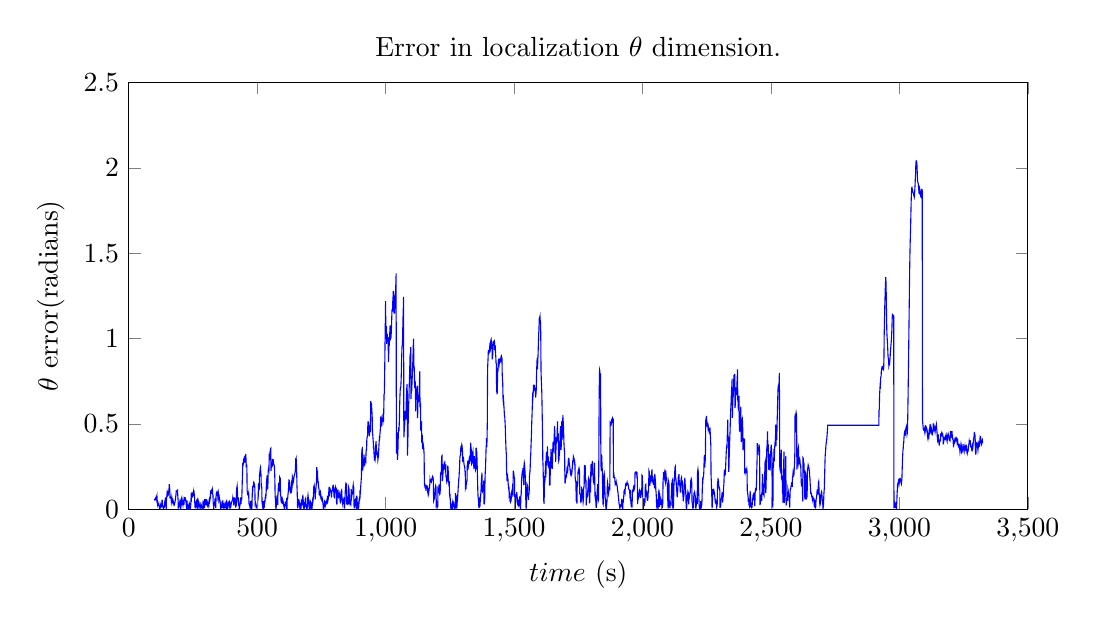
\begin{tikzpicture}

\begin{axis}[
title={Error in localization $\theta$ dimension.},
xlabel={$time$ (s)},
ylabel={$\theta$ error(radians)},
xmin=0, xmax=3500,
ymin=0, ymax=2.5,
axis on top,
width=13cm,
height=7cm
]
\addplot [blue]
coordinates {
(100,0.0592724084854126)
(101,0.0550156831741333)
(102,0.0537326335906982)
(103,0.0623070001602173)
(104,0.0646340847015381)
(105,0.0590170621871948)
(106,0.0578732490539551)
(107,0.0561059713363647)
(108,0.0801171064376831)
(109,0.0634433031082153)
(110,0.0736953020095825)
(111,0.0492959022521973)
(112,0.0307351350784302)
(113,0.0211222171783447)
(114,0.0259432792663574)
(115,0.0282449722290039)
(116,0.0272190570831299)
(117,0.0328972339630127)
(118,0.0208600759506226)
(119,0.0198341608047485)
(120,0.00493550300598145)
(121,0.00728416442871094)
(122,0.0121511220932007)
(123,0.0146913528442383)
(124,0.0224099159240723)
(125,0.00965750217437744)
(126,0.0114129781723022)
(127,0.0163930654525757)
(128,0.0179461240768433)
(129,0.0377165079116821)
(130,0.0555731058120728)
(131,0.0419481992721558)
(132,0.0224950313568115)
(133,0.0121121406555176)
(134,0.0119606256484985)
(135,0.00283777713775635)
(136,0.0133428573608398)
(137,0.011338472366333)
(138,0.00945472717285156)
(139,0.0108567476272583)
(140,0.0359723567962646)
(141,0.0475194454193115)
(142,0.045117974281311)
(143,0.069071888923645)
(144,0.0557403564453125)
(145,0.0263631343841553)
(146,0.000982165336608887)
(147,0.0597293376922607)
(148,0.0692360401153564)
(149,0.0887182950973511)
(150,0.103811860084534)
(151,0.099875807762146)
(152,0.088758111000061)
(153,0.081024169921875)
(154,0.0832598209381104)
(155,0.0989912748336792)
(156,0.107599854469299)
(157,0.122044920921326)
(158,0.146164178848267)
(159,0.125869393348694)
(160,0.114562034606934)
(161,0.0622134208679199)
(162,0.0723897218704224)
(163,0.0690686702728271)
(164,0.0650234222412109)
(165,0.0659371614456177)
(166,0.0418442487716675)
(167,0.0517113208770752)
(168,0.0671892166137695)
(169,0.0562602281570435)
(170,0.0485707521438599)
(171,0.0627973079681396)
(172,0.0466063022613525)
(173,0.0400581359863281)
(174,0.0422776937484741)
(175,0.0329691171646118)
(176,0.0396544933319092)
(177,0.0386953353881836)
(178,0.0310490131378174)
(179,0.0381231307983398)
(180,0.0389789342880249)
(181,0.0491377115249634)
(182,0.0593529939651489)
(183,0.0734015703201294)
(184,0.0844109058380127)
(185,0.104442119598389)
(186,0.103407979011536)
(187,0.102735161781311)
(188,0.108941912651062)
(189,0.108440279960632)
(190,0.110239863395691)
(191,0.0807682275772095)
(192,0.0585089921951294)
(193,0.0066145658493042)
(194,0.0063478946685791)
(195,0.0129826068878174)
(196,0.0175210237503052)
(197,0.0361617803573608)
(198,0.0396593809127808)
(199,0.0449758768081665)
(200,0.0305908918380737)
(201,0.0449920892715454)
(202,0.0237220525741577)
(203,0.000571370124816895)
(204,0.0437582731246948)
(205,0.0610395669937134)
(206,0.0655118227005005)
(207,0.0243905782699585)
(208,0.0338430404663086)
(209,0.0460933446884155)
(210,0.0364576578140259)
(211,0.0269936323165894)
(212,0.0461673736572266)
(213,0.0485078096389771)
(214,0.041589617729187)
(215,0.0547453165054321)
(216,0.0480613708496094)
(217,0.0716115236282349)
(218,0.0527448654174805)
(219,0.0669461488723755)
(220,0.0663059949874878)
(221,0.0611850023269653)
(222,0.0525006055831909)
(223,0.0395171642303467)
(224,0.0262496471405029)
(225,0.0146893262863159)
(226,0.0260225534439087)
(227,0.0514465570449829)
(228,0.0201623439788818)
(229,0.0160202980041504)
(230,0.00125706195831299)
(231,0.0113980770111084)
(232,0.00136983394622803)
(233,0.00671947002410889)
(234,0.00667273998260498)
(235,0.0137171745300293)
(236,0.0327886343002319)
(237,0.0273573398590088)
(238,0.0126820802688599)
(239,0.0186583995819092)
(240,0.00553202629089355)
(241,0.0166100263595581)
(242,0.0422089099884033)
(243,0.0709002017974854)
(244,0.0636031627655029)
(245,0.0900313854217529)
(246,0.0878117084503174)
(247,0.0807353258132935)
(248,0.0891349315643311)
(249,0.0927271842956543)
(250,0.0812774896621704)
(251,0.0851535797119141)
(252,0.0985920429229736)
(253,0.0839213132858276)
(254,0.081393837928772)
(255,0.0895674228668213)
(256,0.0735024213790894)
(257,0.0430172681808472)
(258,0.0142161846160889)
(259,0.00850379467010498)
(260,0.0102980136871338)
(261,0.028123140335083)
(262,0.0354443788528442)
(263,0.0414508581161499)
(264,0.0286768674850464)
(265,0.0415278673171997)
(266,0.0406936407089233)
(267,0.0533492565155029)
(268,0.0568897724151611)
(269,0.00155806541442871)
(270,0.0116053819656372)
(271,0.016484260559082)
(272,0.0367326736450195)
(273,0.0284430980682373)
(274,0.0334174633026123)
(275,0.0257712602615356)
(276,0.0143651962280273)
(277,0.0112775564193726)
(278,0.00125110149383545)
(279,0.0166431665420532)
(280,0.0160917043685913)
(281,0.0314970016479492)
(282,0.0288307666778564)
(283,0.0208761692047119)
(284,0.0109825134277344)
(285,0.00359153747558594)
(286,0.00819599628448486)
(287,0.00988650321960449)
(288,0.00819587707519531)
(289,0.0327873229980469)
(290,0.0264302492141724)
(291,0.0198092460632324)
(292,0.0432884693145752)
(293,0.0470426082611084)
(294,0.0259982347488403)
(295,0.00588405132293701)
(296,0.0232129096984863)
(297,0.029269814491272)
(298,0.0583208799362183)
(299,0.0372036695480347)
(300,0.0364428758621216)
(301,0.0285210609436035)
(302,0.0273504257202148)
(303,0.0597879886627197)
(304,0.0472543239593506)
(305,0.0480685234069824)
(306,0.0435550212860107)
(307,0.0184379816055298)
(308,0.0154075622558594)
(309,0.0355793237686157)
(310,0.0350902080535889)
(311,0.0366290807723999)
(312,0.0292986631393433)
(313,0.0547568798065186)
(314,0.0593169927597046)
(315,0.0637919902801514)
(316,0.0507521629333496)
(317,0.0582067966461182)
(318,0.0722390413284302)
(319,0.106605052947998)
(320,0.107629776000977)
(321,0.105339407920837)
(322,0.0892884731292725)
(323,0.106385111808777)
(324,0.101522445678711)
(325,0.101237177848816)
(326,0.110368251800537)
(327,0.0869197845458984)
(328,0.0812201499938965)
(329,0.0363565683364868)
(330,0.0259304046630859)
(331,0.00143611431121826)
(332,0.0210247039794922)
(333,0.0300658941268921)
(334,0.035888671875)
(335,0.0427109003067017)
(336,0.0635380744934082)
(337,0.0411778688430786)
(338,0.0203253030776978)
(339,0.00742447376251221)
(340,0.0727096796035767)
(341,0.0916533470153809)
(342,0.0958213806152344)
(343,0.0889813899993896)
(344,0.0853490829467773)
(345,0.0991618633270264)
(346,0.0953512191772461)
(347,0.0708096027374268)
(348,0.0797884464263916)
(349,0.0923833847045898)
(350,0.0769584178924561)
(351,0.0495302677154541)
(352,0.0540597438812256)
(353,0.0668082237243652)
(354,0.0576359033584595)
(355,0.0548728704452515)
(356,0.0431673526763916)
(357,0.023795485496521)
(358,0.00134611129760742)
(359,0.00377488136291504)
(360,0.0109531879425049)
(361,0.0148138999938965)
(362,0.0191071033477783)
(363,0.0413377285003662)
(364,0.0439101457595825)
(365,0.00547134876251221)
(366,0.0281717777252197)
(367,0.0334298610687256)
(368,0.0324070453643799)
(369,0.0217106342315674)
(370,0.0116425752639771)
(371,0.0303522348403931)
(372,0.0209392309188843)
(373,0.0138834714889526)
(374,0.00982904434204102)
(375,0.0117224454879761)
(376,0.0277820825576782)
(377,0.03130042552948)
(378,0.0363391637802124)
(379,0.0261207818984985)
(380,0.000916242599487305)
(381,0.0331881046295166)
(382,0.0427528619766235)
(383,0.0343619585037231)
(384,0.0181142091751099)
(385,0.00207877159118652)
(386,0.0197690725326538)
(387,0.0312058925628662)
(388,0.035342812538147)
(389,0.0243240594863892)
(390,0.0485661029815674)
(391,0.0298097133636475)
(392,0.0363271236419678)
(393,0.018369197845459)
(394,0.0246759653091431)
(395,0.00717437267303467)
(396,0.00997591018676758)
(397,0.0252207517623901)
(398,0.0208644866943359)
(399,0.029834508895874)
(400,0.0422537326812744)
(401,0.0423609018325806)
(402,0.0425734519958496)
(403,0.052269458770752)
(404,0.054513692855835)
(405,0.0653225183486938)
(406,0.0517202615737915)
(407,0.0689051151275635)
(408,0.0540915727615356)
(409,0.0225921869277954)
(410,0.0381015539169312)
(411,0.0521100759506226)
(412,0.069305419921875)
(413,0.0534110069274902)
(414,0.0555287599563599)
(415,0.0325111150741577)
(416,0.0138568878173828)
(417,0.0154358148574829)
(418,0.0178549289703369)
(419,0.0259264707565308)
(420,0.120105862617493)
(421,0.125163555145264)
(422,0.135145902633667)
(423,0.114642977714539)
(424,0.0699574947357178)
(425,0.0484442710876465)
(426,0.0412735939025879)
(427,0.0692399740219116)
(428,0.0421832799911499)
(429,0.035977840423584)
(430,0.0021364688873291)
(431,0.000532865524291992)
(432,0.0151406526565552)
(433,0.0232527256011963)
(434,0.0293630361557007)
(435,0.0398198366165161)
(436,0.0683472156524658)
(437,0.0311331748962402)
(438,0.0532656908035278)
(439,0.0580399036407471)
(440,0.0590564012527466)
(441,0.101616263389587)
(442,0.15814733505249)
(443,0.209877252578735)
(444,0.271123290061951)
(445,0.257708549499512)
(446,0.264976382255554)
(447,0.28943943977356)
(448,0.294027090072632)
(449,0.280023455619812)
(450,0.276877164840698)
(451,0.280748724937439)
(452,0.310097217559814)
(453,0.311347007751465)
(454,0.272145509719849)
(455,0.307698249816895)
(456,0.324167490005493)
(457,0.25878643989563)
(458,0.262906551361084)
(459,0.258677363395691)
(460,0.249469995498657)
(461,0.107348322868347)
(462,0.102703928947449)
(463,0.0806310176849365)
(464,0.0935393571853638)
(465,0.0947452783584595)
(466,0.0862846374511719)
(467,0.0938202142715454)
(468,0.0319541692733765)
(469,0.0307812690734863)
(470,0.0231058597564697)
(471,0.0185607671737671)
(472,0.0119131803512573)
(473,0.00255024433135986)
(474,0.0485807657241821)
(475,0.039030909538269)
(476,0.0314364433288574)
(477,0.03639817237854)
(478,0.0147339105606079)
(479,0.00149035453796387)
(480,0.02158522605896)
(481,0.0900906324386597)
(482,0.117250084877014)
(483,0.112078785896301)
(484,0.131473898887634)
(485,0.135984301567078)
(486,0.149224042892456)
(487,0.142781376838684)
(488,0.138638973236084)
(489,0.14667022228241)
(490,0.140519022941589)
(491,0.128520011901855)
(492,0.0366401672363281)
(493,0.0424590110778809)
(494,0.0377684831619263)
(495,0.029771089553833)
(496,0.0072638988494873)
(497,0.00713729858398438)
(498,0.0184204578399658)
(499,0.0179334878921509)
(500,0.0179007053375244)
(501,0.00998044013977051)
(502,0.0474971532821655)
(503,0.0558815002441406)
(504,0.0681053400039673)
(505,0.143954038619995)
(506,0.147075891494751)
(507,0.125016689300537)
(508,0.121311187744141)
(509,0.196770906448364)
(510,0.20930004119873)
(511,0.199747443199158)
(512,0.239012598991394)
(513,0.244744420051575)
(514,0.220318913459778)
(515,0.201860666275024)
(516,0.135242938995361)
(517,0.132193207740784)
(518,0.130064725875854)
(519,0.040247917175293)
(520,0.0307712554931641)
(521,0.0225018262863159)
(522,0.00926470756530762)
(523,0.0179134607315063)
(524,0.034306526184082)
(525,0.0483310222625732)
(526,0.0126819610595703)
(527,0.0210621356964111)
(528,0.0186958312988281)
(529,0.0508022308349609)
(530,0.0353991985321045)
(531,0.0616925954818726)
(532,0.0729668140411377)
(533,0.0805995464324951)
(534,0.0747977495193481)
(535,0.0910190343856812)
(536,0.156064867973328)
(537,0.169530630111694)
(538,0.185162663459778)
(539,0.198338270187378)
(540,0.122584223747253)
(541,0.120434403419495)
(542,0.149844765663147)
(543,0.223947525024414)
(544,0.236485719680786)
(545,0.241780042648315)
(546,0.233837604522705)
(547,0.312535047531128)
(548,0.309444546699524)
(549,0.286454081535339)
(550,0.33493983745575)
(551,0.339209794998169)
(552,0.354560613632202)
(553,0.356736421585083)
(554,0.224608421325684)
(555,0.247959852218628)
(556,0.250988960266113)
(557,0.251700758934021)
(558,0.27494740486145)
(559,0.274733304977417)
(560,0.293199777603149)
(561,0.277484059333801)
(562,0.289570927619934)
(563,0.287620306015015)
(564,0.266264319419861)
(565,0.260910749435425)
(566,0.256162881851196)
(567,0.255955815315247)
(568,0.223082423210144)
(569,0.169259548187256)
(570,0.08092200756073)
(571,0.0569069385528564)
(572,0.0301071405410767)
(573,0.000329971313476562)
(574,0.0101137161254883)
(575,0.0276944637298584)
(576,0.0555201768875122)
(577,0.0708976984024048)
(578,0.0810599327087402)
(579,0.0498713254928589)
(580,0.0256271362304688)
(581,0.0879479646682739)
(582,0.114344239234924)
(583,0.141363263130188)
(584,0.15458071231842)
(585,0.1312655210495)
(586,0.127081036567688)
(587,0.102841258049011)
(588,0.186349749565125)
(589,0.182984828948975)
(590,0.179774641990662)
(591,0.0819954872131348)
(592,0.0761562585830688)
(593,0.0500699281692505)
(594,0.042181134223938)
(595,0.0448861122131348)
(596,0.0511715412139893)
(597,0.0728003978729248)
(598,0.0330464839935303)
(599,0.0319455862045288)
(600,0.031501293182373)
(601,0.0456236600875854)
(602,0.0402895212173462)
(603,0.0317765474319458)
(604,0.015384316444397)
(605,0.0136611461639404)
(606,0.00132441520690918)
(607,0.0297744274139404)
(608,0.019525408744812)
(609,0.0195499658584595)
(610,0.0392856597900391)
(611,0.0381813049316406)
(612,0.0294650793075562)
(613,0.0395522117614746)
(614,0.0107661485671997)
(615,0.00222098827362061)
(616,0.00261104106903076)
(617,0.0560932159423828)
(618,0.0636173486709595)
(619,0.064730167388916)
(620,0.0863560438156128)
(621,0.0985000133514404)
(622,0.11358118057251)
(623,0.152563452720642)
(624,0.170233130455017)
(625,0.169034600257874)
(626,0.151534795761108)
(627,0.120466589927673)
(628,0.124700307846069)
(629,0.124595284461975)
(630,0.0953797101974487)
(631,0.0960910320281982)
(632,0.121037006378174)
(633,0.140579342842102)
(634,0.130323052406311)
(635,0.11842405796051)
(636,0.129525423049927)
(637,0.191334843635559)
(638,0.185870289802551)
(639,0.166059613227844)
(640,0.154613614082336)
(641,0.160571575164795)
(642,0.165766835212708)
(643,0.188295006752014)
(644,0.190959334373474)
(645,0.202306389808655)
(646,0.203362584114075)
(647,0.211212277412415)
(648,0.214913249015808)
(649,0.239558100700378)
(650,0.287675499916077)
(651,0.284709930419922)
(652,0.292495846748352)
(653,0.260212421417236)
(654,0.210389375686646)
(655,0.133438110351562)
(656,0.0952384471893311)
(657,0.0194880962371826)
(658,0.00516128540039062)
(659,0.0308870077133179)
(660,0.0539119243621826)
(661,0.0552214384078979)
(662,0.0380440950393677)
(663,0.0303606986999512)
(664,0.0412105321884155)
(665,0.0327411890029907)
(666,0.0322054624557495)
(667,0.00290632247924805)
(668,0.0107085704803467)
(669,0.0110775232315063)
(670,0.000717639923095703)
(671,0.00885236263275146)
(672,0.0482382774353027)
(673,0.0447438955307007)
(674,0.0560933351516724)
(675,0.0279840230941772)
(676,0.0307327508926392)
(677,0.074409008026123)
(678,0.0773634910583496)
(679,0.0675103664398193)
(680,0.0088731050491333)
(681,0.00671589374542236)
(682,0.00539839267730713)
(683,0.00278007984161377)
(684,0.0219031572341919)
(685,0.0405938625335693)
(686,0.00954580307006836)
(687,0.0580927133560181)
(688,0.0583193302154541)
(689,0.0626707077026367)
(690,0.031086802482605)
(691,0.0270519256591797)
(692,0.0199826955795288)
(693,0.00270426273345947)
(694,0.011773943901062)
(695,0.0180516242980957)
(696,0.0152349472045898)
(697,0.067772388458252)
(698,0.0809751749038696)
(699,0.0667203664779663)
(700,0.0553739070892334)
(701,0.0509489774703979)
(702,0.0293422937393188)
(703,0.0140405893325806)
(704,0.0245835781097412)
(705,0.0245323181152344)
(706,0.0164004564285278)
(707,0.0454263687133789)
(708,0.0412876605987549)
(709,0.0397878885269165)
(710,0.0206484794616699)
(711,0.0120381116867065)
(712,0.0227814912796021)
(713,0.01722252368927)
(714,0.0103065967559814)
(715,0.0364032983779907)
(716,0.0508486032485962)
(717,0.043931245803833)
(718,0.0572025775909424)
(719,0.0626070499420166)
(720,0.130008101463318)
(721,0.133072853088379)
(722,0.138507723808289)
(723,0.117475748062134)
(724,0.114214897155762)
(725,0.116156697273254)
(726,0.0566350221633911)
(727,0.10020923614502)
(728,0.0996483564376831)
(729,0.12571907043457)
(730,0.14223575592041)
(731,0.159868001937866)
(732,0.245822906494141)
(733,0.22839879989624)
(734,0.216521263122559)
(735,0.217592597007751)
(736,0.168752312660217)
(737,0.154272556304932)
(738,0.155555009841919)
(739,0.136141061782837)
(740,0.122104167938232)
(741,0.115494728088379)
(742,0.0808367729187012)
(743,0.0908104181289673)
(744,0.0850592851638794)
(745,0.0964192152023315)
(746,0.101975917816162)
(747,0.0943185091018677)
(748,0.0773836374282837)
(749,0.054587721824646)
(750,0.0673168897628784)
(751,0.0599758625030518)
(752,0.0486595630645752)
(753,0.0463868379592896)
(754,0.0579640865325928)
(755,0.0499610900878906)
(756,0.0370951890945435)
(757,0.0171190500259399)
(758,0.0255080461502075)
(759,0.0186982154846191)
(760,0.00940263271331787)
(761,0.0330765247344971)
(762,0.0122556686401367)
(763,0.0465465784072876)
(764,0.0443402528762817)
(765,0.0435036420822144)
(766,0.0297149419784546)
(767,0.0412145853042603)
(768,0.041287899017334)
(769,0.0363746881484985)
(770,0.0446900129318237)
(771,0.0508600473403931)
(772,0.0450384616851807)
(773,0.0415005683898926)
(774,0.07846999168396)
(775,0.0650637149810791)
(776,0.0545220375061035)
(777,0.0618263483047485)
(778,0.079817533493042)
(779,0.105883717536926)
(780,0.0975093841552734)
(781,0.0746052265167236)
(782,0.125789403915405)
(783,0.124539852142334)
(784,0.117341041564941)
(785,0.111644864082336)
(786,0.109456896781921)
(787,0.0998208522796631)
(788,0.0984833240509033)
(789,0.0681519508361816)
(790,0.0867660045623779)
(791,0.105989694595337)
(792,0.105466365814209)
(793,0.118420600891113)
(794,0.126109957695007)
(795,0.138869762420654)
(796,0.139860987663269)
(797,0.119778394699097)
(798,0.113942384719849)
(799,0.075262188911438)
(800,0.0710140466690063)
(801,0.0690344572067261)
(802,0.104282259941101)
(803,0.121635437011719)
(804,0.119379162788391)
(805,0.126806020736694)
(806,0.11346960067749)
(807,0.123321056365967)
(808,0.119742274284363)
(809,0.0482330322265625)
(810,0.0542519092559814)
(811,0.0282149314880371)
(812,0.11158013343811)
(813,0.111446022987366)
(814,0.0952119827270508)
(815,0.1137775182724)
(816,0.0708664655685425)
(817,0.0680147409439087)
(818,0.0711190700531006)
(819,0.0781340599060059)
(820,0.089018702507019)
(821,0.0803123712539673)
(822,0.0748244524002075)
(823,0.0425179004669189)
(824,0.0394123792648315)
(825,0.0435359477996826)
(826,0.0937374830245972)
(827,0.101198315620422)
(828,0.109578847885132)
(829,0.112213492393494)
(830,0.0779086351394653)
(831,0.047979474067688)
(832,0.0380480289459229)
(833,0.0290391445159912)
(834,0.0479860305786133)
(835,0.042981743812561)
(836,0.0380079746246338)
(837,0.0362534523010254)
(838,0.0609354972839355)
(839,0.0708214044570923)
(840,0.00264227390289307)
(841,0.0329544544219971)
(842,0.0474897623062134)
(843,0.106609702110291)
(844,0.126902461051941)
(845,0.14423680305481)
(846,0.139629483222961)
(847,0.148120522499084)
(848,0.1452876329422)
(849,0.0293369293212891)
(850,0.0294348001480103)
(851,0.065881609916687)
(852,0.0623689889907837)
(853,0.0238463878631592)
(854,0.0361624956130981)
(855,0.0456558465957642)
(856,0.127272844314575)
(857,0.121745109558105)
(858,0.117014408111572)
(859,0.0295116901397705)
(860,0.0441923141479492)
(861,0.0398088693618774)
(862,0.0300167798995972)
(863,0.0371904373168945)
(864,0.0497535467147827)
(865,0.0426799058914185)
(866,0.116968035697937)
(867,0.0970221757888794)
(868,0.0737541913986206)
(869,0.0842492580413818)
(870,0.0867851972579956)
(871,0.0946664810180664)
(872,0.0937860012054443)
(873,0.130990505218506)
(874,0.141719222068787)
(875,0.123496890068054)
(876,0.132473349571228)
(877,0.0250083208084106)
(878,0.00446128845214844)
(879,0.021480917930603)
(880,0.0464123487472534)
(881,0.0432857275009155)
(882,0.0549840927124023)
(883,0.0579758882522583)
(884,0.0427463054656982)
(885,0.0145304203033447)
(886,0.00757122039794922)
(887,0.0756444931030273)
(888,0.0755753517150879)
(889,0.0675476789474487)
(890,0.00957953929901123)
(891,0.0174320936203003)
(892,0.0297151803970337)
(893,0.0324598550796509)
(894,0.0272139310836792)
(895,0.0123896598815918)
(896,0.0194108486175537)
(897,0.0650018453598022)
(898,0.0478636026382446)
(899,0.0497951507568359)
(900,0.0886399745941162)
(901,0.0832185745239258)
(902,0.104313492774963)
(903,0.129522919654846)
(904,0.149841904640198)
(905,0.171795129776001)
(906,0.192469239234924)
(907,0.319016218185425)
(908,0.348514080047607)
(909,0.352781772613525)
(910,0.226402997970581)
(911,0.25003969669342)
(912,0.245540976524353)
(913,0.258669137954712)
(914,0.276747107505798)
(915,0.289743065834045)
(916,0.319687008857727)
(917,0.268200039863586)
(918,0.272078156471252)
(919,0.26384437084198)
(920,0.275156378746033)
(921,0.303712964057922)
(922,0.2874356508255)
(923,0.283138394355774)
(924,0.336825251579285)
(925,0.349406361579895)
(926,0.341095209121704)
(927,0.414807200431824)
(928,0.416941404342651)
(929,0.428807497024536)
(930,0.431772589683533)
(931,0.506309747695923)
(932,0.511563301086426)
(933,0.509520649909973)
(934,0.505305051803589)
(935,0.452619194984436)
(936,0.435721635818481)
(937,0.427146911621094)
(938,0.491018652915955)
(939,0.455072999000549)
(940,0.454246997833252)
(941,0.456318140029907)
(942,0.63377320766449)
(943,0.625714659690857)
(944,0.61348831653595)
(945,0.614662408828735)
(946,0.588367700576782)
(947,0.567093372344971)
(948,0.535295128822327)
(949,0.45003879070282)
(950,0.43592643737793)
(951,0.413997888565063)
(952,0.395797610282898)
(953,0.358410835266113)
(954,0.353933930397034)
(955,0.325076103210449)
(956,0.302352428436279)
(957,0.28407621383667)
(958,0.296866178512573)
(959,0.289667248725891)
(960,0.302922129631042)
(961,0.375093817710876)
(962,0.379674434661865)
(963,0.398829698562622)
(964,0.348955631256104)
(965,0.331331253051758)
(966,0.339594602584839)
(967,0.335605263710022)
(968,0.325449228286743)
(969,0.320458889007568)
(970,0.290106534957886)
(971,0.299818158149719)
(972,0.308640956878662)
(973,0.338859081268311)
(974,0.369482517242432)
(975,0.394922971725464)
(976,0.418696880340576)
(977,0.415932416915894)
(978,0.442023515701294)
(979,0.457659602165222)
(980,0.477542877197266)
(981,0.537691712379456)
(982,0.540372252464294)
(983,0.508587598800659)
(984,0.500725150108337)
(985,0.485457301139832)
(986,0.519633769989014)
(987,0.535399436950684)
(988,0.511943340301514)
(989,0.531654477119446)
(990,0.522687673568726)
(991,0.560928821563721)
(992,0.513040065765381)
(993,0.588249385356903)
(994,0.672585487365723)
(995,0.676762819290161)
(996,0.758498013019562)
(997,0.869450807571411)
(998,0.99370676279068)
(999,1.10469487309456)
(1000,1.21860793232918)
(1001,1.00122731924057)
(1002,1.01954036951065)
(1003,1.07196226716042)
(1004,0.968490868806839)
(1005,1.01621899008751)
(1006,1.01489317417145)
(1007,1.02670495212078)
(1008,0.980336040258408)
(1009,0.991304844617844)
(1010,1.00817151367664)
(1011,0.862033188343048)
(1012,0.90823832526803)
(1013,0.956182979047298)
(1014,0.958198275417089)
(1015,0.993089333176613)
(1016,1.02293248474598)
(1017,1.06549756228924)
(1018,1.07591703534126)
(1019,1.04341970384121)
(1020,1.00127027183771)
(1021,1.00575282797217)
(1022,1.03177586197853)
(1023,1.06506526470184)
(1024,1.12322033941746)
(1025,1.16805233061314)
(1026,1.16982318460941)
(1027,1.1596645116806)
(1028,1.21695831418037)
(1029,1.24300903081894)
(1030,1.27801808714867)
(1031,1.23956996202469)
(1032,1.18699891865253)
(1033,1.14827923476696)
(1034,1.14823098480701)
(1035,1.14972274005413)
(1036,1.20564696192741)
(1037,1.26080188155174)
(1038,1.27192199230194)
(1039,1.27666416764259)
(1040,1.32685667276382)
(1041,1.38182646036148)
(1042,0.326015770435333)
(1043,0.388494670391083)
(1044,0.436422407627106)
(1045,0.449468314647675)
(1046,0.288890689611435)
(1047,0.307458966970444)
(1048,0.344563215970993)
(1049,0.410638034343719)
(1050,0.457197189331055)
(1051,0.479878544807434)
(1052,0.455418050289154)
(1053,0.491231799125671)
(1054,0.537335574626923)
(1055,0.621459186077118)
(1056,0.667683720588684)
(1057,0.701666831970215)
(1058,0.711213111877441)
(1059,0.711780428886414)
(1060,0.738765358924866)
(1061,0.783057689666748)
(1062,0.853707671165466)
(1063,0.908683300018311)
(1064,0.954775214195251)
(1065,0.959331274032593)
(1066,0.990108013153076)
(1067,1.06623303890228)
(1068,1.13066136837006)
(1069,1.1798837184906)
(1070,1.2437961101532)
(1071,0.42030930519104)
(1072,0.438172817230225)
(1073,0.476972341537476)
(1074,0.482402443885803)
(1075,0.514422059059143)
(1076,0.574311375617981)
(1077,0.54350471496582)
(1078,0.524533867835999)
(1079,0.546632885932922)
(1080,0.598819494247437)
(1081,0.650520443916321)
(1082,0.690983176231384)
(1083,0.724149227142334)
(1084,0.73264479637146)
(1085,0.314234495162964)
(1086,0.361346364021301)
(1087,0.421838879585266)
(1088,0.504243969917297)
(1089,0.574036955833435)
(1090,0.620957970619202)
(1091,0.653762459754944)
(1092,0.72267472743988)
(1093,0.771492123603821)
(1094,0.82228147983551)
(1095,0.89107882976532)
(1096,0.907140135765076)
(1097,0.905664324760437)
(1098,0.949496626853943)
(1099,0.646693468093872)
(1100,0.694128036499023)
(1101,0.780711889266968)
(1102,0.691155672073364)
(1103,0.757658958435059)
(1104,0.774278163909912)
(1105,0.827130317687988)
(1106,0.862320423126221)
(1107,0.91468841234316)
(1108,0.970355812703268)
(1109,0.998363796864645)
(1110,0.853592697774069)
(1111,0.819145027791158)
(1112,0.821229283009664)
(1113,0.709011141453878)
(1114,0.751104656849996)
(1115,0.744638983403341)
(1116,0.740124766026632)
(1117,0.572876278554098)
(1118,0.643468205128805)
(1119,0.704229180012838)
(1120,0.676037375126974)
(1121,0.683892313634054)
(1122,0.709631983433859)
(1123,0.724138800297872)
(1124,0.533719364796774)
(1125,0.559246126805441)
(1126,0.669617478047506)
(1127,0.626462284718649)
(1128,0.643487278615133)
(1129,0.640483442937033)
(1130,0.676026884709493)
(1131,0.711132113133566)
(1132,0.755353514348165)
(1133,0.80734616914858)
(1134,0.596841812133789)
(1135,0.61986255645752)
(1136,0.62029242515564)
(1137,0.460612773895264)
(1138,0.479746341705322)
(1139,0.499982118606567)
(1140,0.51448917388916)
(1141,0.386694431304932)
(1142,0.407191514968872)
(1143,0.433884620666504)
(1144,0.353642702102661)
(1145,0.374877452850342)
(1146,0.365272521972656)
(1147,0.374141454696655)
(1148,0.36425518989563)
(1149,0.345693588256836)
(1150,0.319527864456177)
(1151,0.147295475006104)
(1152,0.139642477035522)
(1153,0.150283098220825)
(1154,0.12468695640564)
(1155,0.123425722122192)
(1156,0.134256362915039)
(1157,0.107078313827515)
(1158,0.129964351654053)
(1159,0.134584188461304)
(1160,0.130354881286621)
(1161,0.132085800170898)
(1162,0.126794099807739)
(1163,0.137331962585449)
(1164,0.0971949100494385)
(1165,0.0937504768371582)
(1166,0.0824637413024902)
(1167,0.0885999202728271)
(1168,0.122745037078857)
(1169,0.11048150062561)
(1170,0.122398853302002)
(1171,0.126025676727295)
(1172,0.144619703292847)
(1173,0.172727584838867)
(1174,0.164678812026978)
(1175,0.167213678359985)
(1176,0.16037130355835)
(1177,0.160977363586426)
(1178,0.158403158187866)
(1179,0.167556524276733)
(1180,0.179014205932617)
(1181,0.182592153549194)
(1182,0.18675422668457)
(1183,0.191112995147705)
(1184,0.185548305511475)
(1185,0.185965061187744)
(1186,0.156702041625977)
(1187,0.0471220016479492)
(1188,0.0516073703765869)
(1189,0.0723714828491211)
(1190,0.0582551956176758)
(1191,0.0793220996856689)
(1192,0.0913441181182861)
(1193,0.105358839035034)
(1194,0.133447408676147)
(1195,0.138399124145508)
(1196,0.131051540374756)
(1197,0.0351135730743408)
(1198,0.0419507026672363)
(1199,0.0269491672515869)
(1200,0.00281214714050293)
(1201,0.0212507247924805)
(1202,0.0135807991027832)
(1203,0.0151352882385254)
(1204,0.113699436187744)
(1205,0.108190298080444)
(1206,0.111691236495972)
(1207,0.124853134155273)
(1208,0.115124464035034)
(1209,0.134541511535645)
(1210,0.137717723846436)
(1211,0.089055061340332)
(1212,0.0922050476074219)
(1213,0.118157625198364)
(1214,0.204301834106445)
(1215,0.201644420623779)
(1216,0.206365346908569)
(1217,0.226444125175476)
(1218,0.299308896064758)
(1219,0.311831474304199)
(1220,0.313724637031555)
(1221,0.166393518447876)
(1222,0.181482553482056)
(1223,0.201910614967346)
(1224,0.221358776092529)
(1225,0.239618182182312)
(1226,0.252288103103638)
(1227,0.247138500213623)
(1228,0.233303070068359)
(1229,0.265297770500183)
(1230,0.259415745735168)
(1231,0.264520525932312)
(1232,0.240296959877014)
(1233,0.249099969863892)
(1234,0.2621009349823)
(1235,0.191933155059814)
(1236,0.188645958900452)
(1237,0.170409917831421)
(1238,0.18192994594574)
(1239,0.177434802055359)
(1240,0.190170049667358)
(1241,0.182068109512329)
(1242,0.254863381385803)
(1243,0.245332479476929)
(1244,0.217655658721924)
(1245,0.170756459236145)
(1246,0.153584003448486)
(1247,0.160847187042236)
(1248,0.160784482955933)
(1249,0.0846295356750488)
(1250,0.0746386051177979)
(1251,0.0776853561401367)
(1252,0.0507657527923584)
(1253,0.0239157676696777)
(1254,0.00483107566833496)
(1255,0.0159592628479004)
(1256,0.0318481922149658)
(1257,0.014960765838623)
(1258,0.00533747673034668)
(1259,0.0198237895965576)
(1260,0.0135886669158936)
(1261,0.0342874526977539)
(1262,0.0247631072998047)
(1263,0.0174582004547119)
(1264,0.0187208652496338)
(1265,0.0296962261199951)
(1266,0.0177450180053711)
(1267,0.00874614715576172)
(1268,0.0119011402130127)
(1269,0.000654458999633789)
(1270,0.000379085540771484)
(1271,0.010624885559082)
(1272,0.0933725833892822)
(1273,0.0732436180114746)
(1274,0.0744225978851318)
(1275,0.075098991394043)
(1276,0.00883340835571289)
(1277,0.0074775218963623)
(1278,0.0238990783691406)
(1279,0.0457179546356201)
(1280,0.0496208667755127)
(1281,0.0862345695495605)
(1282,0.107789754867554)
(1283,0.133806705474854)
(1284,0.149967789649963)
(1285,0.178468227386475)
(1286,0.188184499740601)
(1287,0.2182776927948)
(1288,0.245441794395447)
(1289,0.293250679969788)
(1290,0.311888337135315)
(1291,0.314866185188293)
(1292,0.317470550537109)
(1293,0.370065569877625)
(1294,0.359233498573303)
(1295,0.360383987426758)
(1296,0.370379447937012)
(1297,0.356825232505798)
(1298,0.363721609115601)
(1299,0.349844574928284)
(1300,0.286712527275085)
(1301,0.289818644523621)
(1302,0.303743362426758)
(1303,0.300795793533325)
(1304,0.284531235694885)
(1305,0.267641425132751)
(1306,0.256811261177063)
(1307,0.252593755722046)
(1308,0.247803092002869)
(1309,0.222378134727478)
(1310,0.221061706542969)
(1311,0.123509883880615)
(1312,0.128774166107178)
(1313,0.117823839187622)
(1314,0.149815559387207)
(1315,0.149412751197815)
(1316,0.164229989051819)
(1317,0.165892601013184)
(1318,0.257221460342407)
(1319,0.269527435302734)
(1320,0.283849120140076)
(1321,0.231473922729492)
(1322,0.255204677581787)
(1323,0.255053043365479)
(1324,0.275589346885681)
(1325,0.2879718542099)
(1326,0.275423526763916)
(1327,0.273086071014404)
(1328,0.302529454231262)
(1329,0.310972452163696)
(1330,0.280011773109436)
(1331,0.389870762825012)
(1332,0.367950439453125)
(1333,0.353055834770203)
(1334,0.344693899154663)
(1335,0.263935685157776)
(1336,0.267116904258728)
(1337,0.283841729164124)
(1338,0.32857871055603)
(1339,0.325697660446167)
(1340,0.334396839141846)
(1341,0.292497158050537)
(1342,0.273913383483887)
(1343,0.256817221641541)
(1344,0.23683500289917)
(1345,0.310441493988037)
(1346,0.29369854927063)
(1347,0.284157633781433)
(1348,0.295179009437561)
(1349,0.242060422897339)
(1350,0.228870749473572)
(1351,0.234515428543091)
(1352,0.356361389160156)
(1353,0.356829404830933)
(1354,0.316889762878418)
(1355,0.338141798973083)
(1356,0.281958818435669)
(1357,0.234676361083984)
(1358,0.167623281478882)
(1359,0.107061386108398)
(1360,0.0708396434783936)
(1361,0.0594766139984131)
(1362,0.0450408458709717)
(1363,0.0101652145385742)
(1364,0.00941729545593262)
(1365,0.014655590057373)
(1366,0.0496885776519775)
(1367,0.0431182384490967)
(1368,0.03554368019104)
(1369,0.0611839294433594)
(1370,0.0774188041687012)
(1371,0.0988848209381104)
(1372,0.12454628944397)
(1373,0.179341077804565)
(1374,0.18076491355896)
(1375,0.213625192642212)
(1376,0.106842279434204)
(1377,0.102562189102173)
(1378,0.110329389572144)
(1379,0.136486291885376)
(1380,0.103219509124756)
(1381,0.128271579742432)
(1382,0.167659759521484)
(1383,0.0318944454193115)
(1384,0.031013011932373)
(1385,0.0425617694854736)
(1386,0.0655941963195801)
(1387,0.176403284072876)
(1388,0.218061685562134)
(1389,0.240079402923584)
(1390,0.291545391082764)
(1391,0.348177433013916)
(1392,0.371552228927612)
(1393,0.416536569595337)
(1394,0.363610982894897)
(1395,0.414027690887451)
(1396,0.510804891586304)
(1397,0.817831039428711)
(1398,0.856257438659668)
(1399,0.88613224029541)
(1400,0.928617238998413)
(1401,0.929106950759888)
(1402,0.925470113754272)
(1403,0.921313762664795)
(1404,0.931226968765259)
(1405,0.947701215744019)
(1406,0.935165882110596)
(1407,0.918379068374634)
(1408,0.969358444213867)
(1409,0.977514743804932)
(1410,0.992379426956177)
(1411,0.995861530303955)
(1412,0.940027236938477)
(1413,0.952098369598389)
(1414,0.982004165649414)
(1415,0.877426147460938)
(1416,0.889589071273804)
(1417,0.902528047561646)
(1418,0.93909764289856)
(1419,0.958670679722921)
(1420,0.961795155202047)
(1421,0.981327597294943)
(1422,0.983284775410787)
(1423,0.986802164708273)
(1424,0.981978956853048)
(1425,0.931221787129537)
(1426,0.946389261876242)
(1427,0.949153486882345)
(1428,0.917979303990499)
(1429,0.890975952148438)
(1430,0.856316328048706)
(1431,0.851859331130981)
(1432,0.725496053695679)
(1433,0.683913707733154)
(1434,0.678265810012817)
(1435,0.680288791656494)
(1436,0.828416585922241)
(1437,0.807198286056519)
(1438,0.815209150314331)
(1439,0.875064611434937)
(1440,0.876911401748657)
(1441,0.859692335128784)
(1442,0.849053621292114)
(1443,0.862308502197266)
(1444,0.877199172973633)
(1445,0.878358602523804)
(1446,0.872572660446167)
(1447,0.859099149703979)
(1448,0.879560470581055)
(1449,0.891032695770264)
(1450,0.895414113998413)
(1451,0.885655403137207)
(1452,0.890238046646118)
(1453,0.882680177688599)
(1454,0.790076017379761)
(1455,0.755979299545288)
(1456,0.739495038986206)
(1457,0.653056859970093)
(1458,0.634389877319336)
(1459,0.64408540725708)
(1460,0.624154329299927)
(1461,0.594507694244385)
(1462,0.567316770553589)
(1463,0.544330358505249)
(1464,0.538643360137939)
(1465,0.510079383850098)
(1466,0.476056814193726)
(1467,0.427046775817871)
(1468,0.381081342697144)
(1469,0.342408180236816)
(1470,0.324307680130005)
(1471,0.232807636260986)
(1472,0.193135738372803)
(1473,0.163210391998291)
(1474,0.207879066467285)
(1475,0.188436985015869)
(1476,0.184359550476074)
(1477,0.154858350753784)
(1478,0.136810779571533)
(1479,0.115961790084839)
(1480,0.136083126068115)
(1481,0.0786542892456055)
(1482,0.083153247833252)
(1483,0.100775480270386)
(1484,0.0476903915405273)
(1485,0.0464816093444824)
(1486,0.0429413318634033)
(1487,0.0566000938415527)
(1488,0.0643222332000732)
(1489,0.0602383613586426)
(1490,0.0839059352874756)
(1491,0.0741102695465088)
(1492,0.0752301216125488)
(1493,0.0836329460144043)
(1494,0.11975884437561)
(1495,0.110882520675659)
(1496,0.103886604309082)
(1497,0.224795341491699)
(1498,0.211516857147217)
(1499,0.183259963989258)
(1500,0.195423603057861)
(1501,0.181654930114746)
(1502,0.180926084518433)
(1503,0.0160033702850342)
(1504,0.0110151767730713)
(1505,0.00882434844970703)
(1506,0.0542855262756348)
(1507,0.0825645923614502)
(1508,0.0827407836914062)
(1509,0.0844132900238037)
(1510,0.0906977653503418)
(1511,0.0997688770294189)
(1512,0.0523655414581299)
(1513,0.0419802665710449)
(1514,0.0512793064117432)
(1515,0.0398697853088379)
(1516,0.056584358215332)
(1517,0.0311243534088135)
(1518,0.0159952640533447)
(1519,0.0460076332092285)
(1520,0.0304460525512695)
(1521,0.0378637313842773)
(1522,0.0746383666992188)
(1523,0.0539793968200684)
(1524,0.0275833606719971)
(1525,0.00156211853027344)
(1526,0.0376706123352051)
(1527,0.080082893371582)
(1528,0.0899193286895752)
(1529,0.16598916053772)
(1530,0.186132431030273)
(1531,0.202377557754517)
(1532,0.217006683349609)
(1533,0.217788457870483)
(1534,0.226992130279541)
(1535,0.240378379821777)
(1536,0.198408603668213)
(1537,0.167290687561035)
(1538,0.141114950180054)
(1539,0.259036779403687)
(1540,0.270651817321777)
(1541,0.260970830917358)
(1542,0.232741832733154)
(1543,0.220052003860474)
(1544,0.177878141403198)
(1545,0.135235071182251)
(1546,0.035428524017334)
(1547,0.00591754913330078)
(1548,0.0157811641693115)
(1549,0.0685851573944092)
(1550,0.0964813232421875)
(1551,0.143845796585083)
(1552,0.13968563079834)
(1553,0.0973117351531982)
(1554,0.0925760269165039)
(1555,0.088207483291626)
(1556,0.0537848472595215)
(1557,0.0814113616943359)
(1558,0.0881087779998779)
(1559,0.106197118759155)
(1560,0.189470291137695)
(1561,0.207406759262085)
(1562,0.219631671905518)
(1563,0.248220920562744)
(1564,0.301573514938354)
(1565,0.319348812103271)
(1566,0.365441560745239)
(1567,0.403242826461792)
(1568,0.45237135887146)
(1569,0.511569738388062)
(1570,0.548089265823364)
(1571,0.597033739089966)
(1572,0.653919458389282)
(1573,0.645458698272705)
(1574,0.66660213470459)
(1575,0.695569515228271)
(1576,0.728849172592163)
(1577,0.717361211776733)
(1578,0.710424661636353)
(1579,0.71747875213623)
(1580,0.728228569030762)
(1581,0.693660259246826)
(1582,0.693031311035156)
(1583,0.69269847869873)
(1584,0.653689384460449)
(1585,0.670629739761353)
(1586,0.683787107467651)
(1587,0.723841905593872)
(1588,0.815533638000488)
(1589,0.848986864089966)
(1590,0.88629412651062)
(1591,0.81851560274233)
(1592,0.850908342991964)
(1593,0.883707586918966)
(1594,0.927326265965597)
(1595,0.985416475926534)
(1596,1.03354770341982)
(1597,1.04691440263857)
(1598,1.11969334283938)
(1599,1.10135990778078)
(1600,1.12335116067995)
(1601,1.13068539301027)
(1602,1.104469601308)
(1603,1.09723884264101)
(1604,1.03028089204897)
(1605,0.814494673405783)
(1606,0.763503138219015)
(1607,0.726570431386129)
(1608,0.689362049102783)
(1609,0.611183881759644)
(1610,0.522158145904541)
(1611,0.421426773071289)
(1612,0.2860267162323)
(1613,0.254498481750488)
(1614,0.18010687828064)
(1615,0.126284837722778)
(1616,0.0352051258087158)
(1617,0.0348954200744629)
(1618,0.114420890808105)
(1619,0.193107604980469)
(1620,0.155803918838501)
(1621,0.195085763931274)
(1622,0.243047714233398)
(1623,0.280800700187683)
(1624,0.185864090919495)
(1625,0.279671430587769)
(1626,0.335956931114197)
(1627,0.268995642662048)
(1628,0.26616108417511)
(1629,0.307340502738953)
(1630,0.367377400398254)
(1631,0.271075487136841)
(1632,0.30403459072113)
(1633,0.304839372634888)
(1634,0.258285522460938)
(1635,0.247822403907776)
(1636,0.249843955039978)
(1637,0.280215620994568)
(1638,0.138282775878906)
(1639,0.160498738288879)
(1640,0.14116632938385)
(1641,0.215072989463806)
(1642,0.253115773200989)
(1643,0.299992680549622)
(1644,0.351778268814087)
(1645,0.238858699798584)
(1646,0.288852095603943)
(1647,0.2980135679245)
(1648,0.334022998809814)
(1649,0.235400199890137)
(1650,0.297741174697876)
(1651,0.361396670341492)
(1652,0.393439292907715)
(1653,0.363527178764343)
(1654,0.362829208374023)
(1655,0.354300260543823)
(1656,0.41291081905365)
(1657,0.452697515487671)
(1658,0.486101925373077)
(1659,0.408083915710449)
(1660,0.412437915802002)
(1661,0.414251387119293)
(1662,0.276566088199615)
(1663,0.341251313686371)
(1664,0.382888972759247)
(1665,0.395773768424988)
(1666,0.411245882511139)
(1667,0.407048583030701)
(1668,0.446785151958466)
(1669,0.513776302337646)
(1670,0.40705817937851)
(1671,0.436216711997986)
(1672,0.444183588027954)
(1673,0.297828018665314)
(1674,0.283223152160645)
(1675,0.291198432445526)
(1676,0.34587574005127)
(1677,0.338874876499176)
(1678,0.38862270116806)
(1679,0.385388195514679)
(1680,0.455906510353088)
(1681,0.476925522089005)
(1682,0.48650798201561)
(1683,0.346932142972946)
(1684,0.376551538705826)
(1685,0.437394917011261)
(1686,0.517050176858902)
(1687,0.405010595917702)
(1688,0.436326071619987)
(1689,0.437273651361465)
(1690,0.552363246679306)
(1691,0.522489577531815)
(1692,0.498262077569962)
(1693,0.462162017822266)
(1694,0.396611630916595)
(1695,0.365258723497391)
(1696,0.343356221914291)
(1697,0.325832664966583)
(1698,0.160128593444824)
(1699,0.149860471487045)
(1700,0.183733135461807)
(1701,0.189754664897919)
(1702,0.183401644229889)
(1703,0.190115690231323)
(1704,0.189997315406799)
(1705,0.21190145611763)
(1706,0.234449803829193)
(1707,0.249701946973801)
(1708,0.233283400535583)
(1709,0.226576685905457)
(1710,0.253422051668167)
(1711,0.278345584869385)
(1712,0.299600690603256)
(1713,0.283575266599655)
(1714,0.287068888545036)
(1715,0.267360389232635)
(1716,0.257331103086472)
(1717,0.25017261505127)
(1718,0.229754656553268)
(1719,0.228747963905334)
(1720,0.209887206554413)
(1721,0.200287133455276)
(1722,0.196620970964432)
(1723,0.202094316482544)
(1724,0.214847683906555)
(1725,0.202027499675751)
(1726,0.237679004669189)
(1727,0.239360317587852)
(1728,0.276494368910789)
(1729,0.284067928791046)
(1730,0.285108730196953)
(1731,0.30845582485199)
(1732,0.303534165024757)
(1733,0.290614455938339)
(1734,0.279683515429497)
(1735,0.286398112773895)
(1736,0.279620304703712)
(1737,0.273147225379944)
(1738,0.187291875481606)
(1739,0.169764548540115)
(1740,0.16933411359787)
(1741,0.1456358730793)
(1742,0.050195038318634)
(1743,0.049878865480423)
(1744,0.0424909889698029)
(1745,0.0331538021564484)
(1746,0.162154912948608)
(1747,0.138646692037582)
(1748,0.146367192268372)
(1749,0.217020511627197)
(1750,0.224728941917419)
(1751,0.227470904588699)
(1752,0.233510673046112)
(1753,0.240400940179825)
(1754,0.232110559940338)
(1755,0.212728947401047)
(1756,0.0900229215621948)
(1757,0.0867587029933929)
(1758,0.0850065946578979)
(1759,0.066380500793457)
(1760,0.0399661064147949)
(1761,0.0412612557411194)
(1762,0.0529104471206665)
(1763,0.103713899850845)
(1764,0.0951845049858093)
(1765,0.11627659201622)
(1766,0.113050073385239)
(1767,0.0639707446098328)
(1768,0.0605205595493317)
(1769,0.0411467552185059)
(1770,0.052055835723877)
(1771,0.120432436466217)
(1772,0.131878674030304)
(1773,0.132917582988739)
(1774,0.25909635424614)
(1775,0.234911888837814)
(1776,0.234816372394562)
(1777,0.256433993577957)
(1778,0.180759608745575)
(1779,0.158167749643326)
(1780,0.171854585409164)
(1781,0.0221284925937653)
(1782,0.0552242398262024)
(1783,0.0702890753746033)
(1784,0.0793095529079437)
(1785,0.0730015933513641)
(1786,0.0775054693222046)
(1787,0.107103496789932)
(1788,0.12188920378685)
(1789,0.157770782709122)
(1790,0.175201147794724)
(1791,0.166951268911362)
(1792,0.12451496720314)
(1793,0.0806654095649719)
(1794,0.0343560874462128)
(1795,0.0437800884246826)
(1796,0.18274761736393)
(1797,0.144564673304558)
(1798,0.0989773124456406)
(1799,0.241530686616898)
(1800,0.26556009054184)
(1801,0.247624665498734)
(1802,0.207882076501846)
(1803,0.215082466602325)
(1804,0.260136991739273)
(1805,0.282415002584457)
(1806,0.247500628232956)
(1807,0.212313503026962)
(1808,0.186697870492935)
(1809,0.154874593019485)
(1810,0.167889297008514)
(1811,0.156682103872299)
(1812,0.142370015382767)
(1813,0.272285461425781)
(1814,0.190088033676147)
(1815,0.0813370943069458)
(1816,0.0681358575820923)
(1817,0.0771299600601196)
(1818,0.0555878877639771)
(1819,0.0204149484634399)
(1820,0.00813555717468262)
(1821,0.0424227714538574)
(1822,0.0609146952629089)
(1823,0.0811890363693237)
(1824,0.11654132604599)
(1825,0.131317555904388)
(1826,0.148231863975525)
(1827,0.0867879390716553)
(1828,0.0514553189277649)
(1829,0.0577413439750671)
(1830,0.287755310535431)
(1831,0.552411153912544)
(1832,0.739006247371435)
(1833,0.816606996580958)
(1834,0.810367439873517)
(1835,0.780889466404915)
(1836,0.767596004530787)
(1837,0.77320141531527)
(1838,0.261290034279227)
(1839,0.244642980396748)
(1840,0.223251447081566)
(1841,0.321039281785488)
(1842,0.283092468976974)
(1843,0.247226014733315)
(1844,0.204058364033699)
(1845,0.102566838264465)
(1846,0.0315470993518829)
(1847,0.0271241664886475)
(1848,0.0584917962551117)
(1849,0.194770187139511)
(1850,0.202448695898056)
(1851,0.209765762090683)
(1852,0.194028556346893)
(1853,0.129132956266403)
(1854,0.0950250923633575)
(1855,0.0634676516056061)
(1856,0.0372394621372223)
(1857,0.0180400311946869)
(1858,0.00172513723373413)
(1859,0.0262467265129089)
(1860,0.0169714689254761)
(1861,0.0305188894271851)
(1862,0.0490061640739441)
(1863,0.129682987928391)
(1864,0.157665774226189)
(1865,0.148621812462807)
(1866,0.117674916982651)
(1867,0.0968642830848694)
(1868,0.0887554883956909)
(1869,0.101094126701355)
(1870,0.116889610886574)
(1871,0.12200129032135)
(1872,0.135398268699646)
(1873,0.130026459693909)
(1874,0.505450621247292)
(1875,0.501593217253685)
(1876,0.512275129556656)
(1877,0.486978933215141)
(1878,0.498134076595306)
(1879,0.515088364481926)
(1880,0.509920135140419)
(1881,0.517110213637352)
(1882,0.525346010923386)
(1883,0.531249150633812)
(1884,0.520035207271576)
(1885,0.524317786097527)
(1886,0.532047554850578)
(1887,0.182368397712708)
(1888,0.195042863488197)
(1889,0.199966549873352)
(1890,0.18570339679718)
(1891,0.184100791811943)
(1892,0.184247940778732)
(1893,0.161300182342529)
(1894,0.145803049206734)
(1895,0.150140523910522)
(1896,0.147782564163208)
(1897,0.146198004484177)
(1898,0.156094297766685)
(1899,0.144406735897064)
(1900,0.145445585250854)
(1901,0.138660922646523)
(1902,0.131385624408722)
(1903,0.112841606140137)
(1904,0.102929398417473)
(1905,0.0930357277393341)
(1906,0.0723752677440643)
(1907,0.0631438195705414)
(1908,0.0457189679145813)
(1909,0.0287769734859467)
(1910,0.0266193151473999)
(1911,0.0128657519817352)
(1912,0.00392121076583862)
(1913,0.0122789144515991)
(1914,0.0236455202102661)
(1915,0.0226928293704987)
(1916,0.0241732597351074)
(1917,0.0198928117752075)
(1918,0.0256791412830353)
(1919,0.0567937195301056)
(1920,0.0569494664669037)
(1921,0.0418555736541748)
(1922,0.0176252126693726)
(1923,0.00226312875747681)
(1924,0.0367393791675568)
(1925,0.0404401123523712)
(1926,0.0549042820930481)
(1927,0.0731016993522644)
(1928,0.0993757545948029)
(1929,0.0978576689958572)
(1930,0.117349162697792)
(1931,0.102875486016273)
(1932,0.0965687781572342)
(1933,0.122832149267197)
(1934,0.141542911529541)
(1935,0.148790821433067)
(1936,0.14728419482708)
(1937,0.146905168890953)
(1938,0.143576815724373)
(1939,0.153072640299797)
(1940,0.158108487725258)
(1941,0.149500370025635)
(1942,0.14403860270977)
(1943,0.143451392650604)
(1944,0.145438745617867)
(1945,0.135872215032578)
(1946,0.12300518155098)
(1947,0.116376727819443)
(1948,0.114482492208481)
(1949,0.11335563659668)
(1950,0.109678938984871)
(1951,0.0823907256126404)
(1952,0.0894242227077484)
(1953,0.112219735980034)
(1954,0.0594195872545242)
(1955,0.0376335233449936)
(1956,0.022903174161911)
(1957,0.0248929560184479)
(1958,0.0142480880022049)
(1959,0.0127430707216263)
(1960,0.0473820716142654)
(1961,0.104656293988228)
(1962,0.102003403007984)
(1963,0.106180362403393)
(1964,0.115962892770767)
(1965,0.105653487145901)
(1966,0.10703980922699)
(1967,0.134528674185276)
(1968,0.13740997761488)
(1969,0.122919738292694)
(1970,0.129419796168804)
(1971,0.211435578763485)
(1972,0.215712912380695)
(1973,0.216623738408089)
(1974,0.208065524697304)
(1975,0.208005405962467)
(1976,0.217425845563412)
(1977,0.21623057872057)
(1978,0.198131293058395)
(1979,0.202556766569614)
(1980,0.173946492373943)
(1981,0.0292310416698456)
(1982,0.0585267320275307)
(1983,0.0662026107311249)
(1984,0.063968263566494)
(1985,0.0746641010046005)
(1986,0.0877819955348969)
(1987,0.0973260104656219)
(1988,0.0883402153849602)
(1989,0.0991776511073112)
(1990,0.0818432793021202)
(1991,0.0819979757070541)
(1992,0.0806972831487656)
(1993,0.0651940703392029)
(1994,0.0953332111239433)
(1995,0.0900484994053841)
(1996,0.0903511419892311)
(1997,0.0818586423993111)
(1998,0.19841630011797)
(1999,0.196277260780334)
(2000,0.160859525203705)
(2001,0.0397247970104218)
(2002,0.0117213428020477)
(2003,0.00371241569519043)
(2004,0.06278445571661)
(2005,0.0394671037793159)
(2006,0.031383715569973)
(2007,0.0183568969368935)
(2008,0.0395216047763824)
(2009,0.0500040724873543)
(2010,0.0381516441702843)
(2011,0.130689471960068)
(2012,0.144457451999187)
(2013,0.145948484539986)
(2014,0.0842178165912628)
(2015,0.0874902904033661)
(2016,0.0880081504583359)
(2017,0.106516029685736)
(2018,0.0538049973547459)
(2019,0.0529272817075253)
(2020,0.0523415803909302)
(2021,0.0550660602748394)
(2022,0.0913886111229658)
(2023,0.101185839623213)
(2024,0.113310515880585)
(2025,0.223986607044935)
(2026,0.218910813331604)
(2027,0.218704119324684)
(2028,0.136422902345657)
(2029,0.144757766276598)
(2030,0.166393060237169)
(2031,0.166821144521236)
(2032,0.179277963936329)
(2033,0.172487311065197)
(2034,0.181103281676769)
(2035,0.189807020127773)
(2036,0.216919131577015)
(2037,0.23246656358242)
(2038,0.174999728798866)
(2039,0.182661518454552)
(2040,0.170568123459816)
(2041,0.161245748400688)
(2042,0.170854121446609)
(2043,0.15917843580246)
(2044,0.152379281818867)
(2045,0.143548309803009)
(2046,0.142091535031796)
(2047,0.122277095913887)
(2048,0.205726318061352)
(2049,0.190763980150223)
(2050,0.168149642646313)
(2051,0.151414770167321)
(2052,0.109127971343696)
(2053,0.0997968011070043)
(2054,0.0688713490962982)
(2055,0.0266397288069129)
(2056,0.0351086361333728)
(2057,0.0520234620198607)
(2058,0.0535868657752872)
(2059,0.00516078993678093)
(2060,0.0162909142673016)
(2061,0.000704325735569)
(2062,0.0699329786002636)
(2063,0.100295149721205)
(2064,0.107945185678545)
(2065,0.102767458651215)
(2066,0.0137530099600554)
(2067,0.0242688041180372)
(2068,0.0425328817218542)
(2069,0.0427912436425686)
(2070,0.0547211281955242)
(2071,0.0640735365450382)
(2072,0.0402793027460575)
(2073,0.0248536542057991)
(2074,0.0460166707634926)
(2075,0.0483325347304344)
(2076,0.00785140693187714)
(2077,0.00958290696144104)
(2078,0.0205789506435394)
(2079,0.0356753766536713)
(2080,0.157334830611944)
(2081,0.181407105177641)
(2082,0.218555714935064)
(2083,0.186238549649715)
(2084,0.189172767102718)
(2085,0.209426425397396)
(2086,0.215834818780422)
(2087,0.168893188238144)
(2088,0.168663084506989)
(2089,0.160794168710709)
(2090,0.226517520844936)
(2091,0.214381329715252)
(2092,0.200928144156933)
(2093,0.165489159524441)
(2094,0.189227856695652)
(2095,0.159628041088581)
(2096,0.152349896728992)
(2097,0.142937295138836)
(2098,0.0634578093886375)
(2099,0.0341508165001869)
(2100,0.00334461778402328)
(2101,0.141658887267113)
(2102,0.160079501569271)
(2103,0.150904983282089)
(2104,0.00889196246862411)
(2105,0.0280886590480804)
(2106,0.0220661461353302)
(2107,0.0332338884472847)
(2108,0.0244007930159569)
(2109,0.0397139713168144)
(2110,0.0248110517859459)
(2111,0.0246224626898766)
(2112,0.0716725662350655)
(2113,0.105953864753246)
(2114,0.150038689374924)
(2115,0.151081429794431)
(2116,0.167311119847)
(2117,0.17127058794722)
(2118,0.017653439193964)
(2119,0.0214077290147543)
(2120,0.0113511439412832)
(2121,0.0193950273096561)
(2122,0.126033013686538)
(2123,0.153729888610542)
(2124,0.173135861754417)
(2125,0.184128440916538)
(2126,0.23288076557219)
(2127,0.246715109795332)
(2128,0.250420492142439)
(2129,0.188937805593014)
(2130,0.167560074478388)
(2131,0.168070568703115)
(2132,0.129774348810315)
(2133,0.118436509743333)
(2134,0.0937797240912914)
(2135,0.0688845440745354)
(2136,0.0856373310089111)
(2137,0.106518223881721)
(2138,0.132752161473036)
(2139,0.178247313946486)
(2140,0.175437226891518)
(2141,0.189931839704514)
(2142,0.204876612871885)
(2143,0.142768528312445)
(2144,0.155037450604141)
(2145,0.141504723578691)
(2146,0.14021865464747)
(2147,0.0978652872145176)
(2148,0.111536665819585)
(2149,0.0976644065231085)
(2150,0.168787130154669)
(2151,0.180829030927271)
(2152,0.185659126378596)
(2153,0.165572359226644)
(2154,0.151403827476315)
(2155,0.166152266785502)
(2156,0.144454868044704)
(2157,0.0883220979012549)
(2158,0.0721131386235356)
(2159,0.0462639555335045)
(2160,0.0923656523227692)
(2161,0.0777430236339569)
(2162,0.0887003466486931)
(2163,0.15605029463768)
(2164,0.162446551024914)
(2165,0.184152139350772)
(2166,0.146748347207904)
(2167,0.139678405597806)
(2168,0.120349075645208)
(2169,0.070373497903347)
(2170,0.0156315118074417)
(2171,0.0181407481431961)
(2172,0.00201348960399628)
(2173,0.0792961642146111)
(2174,0.0788329020142555)
(2175,0.0689273476600647)
(2176,0.0888951048254967)
(2177,0.102609053254128)
(2178,0.0978260859847069)
(2179,0.0914424285292625)
(2180,0.0280930697917938)
(2181,0.0576794072985649)
(2182,0.0640223100781441)
(2183,0.0749796107411385)
(2184,0.0886014997959137)
(2185,0.0936803072690964)
(2186,0.0957101956009865)
(2187,0.137805983424187)
(2188,0.167228234931827)
(2189,0.170608377084136)
(2190,0.178546680137515)
(2191,0.174377316609025)
(2192,0.146717429161072)
(2193,0.0393534079194069)
(2194,0.0377205535769463)
(2195,0.0197214335203171)
(2196,0.00682142376899719)
(2197,0.0126309990882874)
(2198,0.0183356925845146)
(2199,0.00629743933677673)
(2200,0.0924816727638245)
(2201,0.0947204679250717)
(2202,0.0928564071655273)
(2203,0.0985346138477325)
(2204,0.0854304581880569)
(2205,0.0790121257305145)
(2206,0.0758169442415237)
(2207,0.0103962793946266)
(2208,0.00733687728643417)
(2209,0.0194491967558861)
(2210,0.0271490216255188)
(2211,0.0472298339009285)
(2212,0.0419803559780121)
(2213,0.030021458864212)
(2214,0.210470125079155)
(2215,0.222438223659992)
(2216,0.233203761279583)
(2217,0.219889387488365)
(2218,0.113153010606766)
(2219,0.0870051085948944)
(2220,0.050214022397995)
(2221,0.0197863578796387)
(2222,0.00771497189998627)
(2223,0.00847338140010834)
(2224,0.0031311959028244)
(2225,0.0110315829515457)
(2226,0.0194122940301895)
(2227,0.0464247018098831)
(2228,0.00707554817199707)
(2229,0.0106631517410278)
(2230,0.0219366252422333)
(2231,0.0296767354011536)
(2232,0.0608641803264618)
(2233,0.128417551517487)
(2234,0.167938828468323)
(2235,0.163211464881897)
(2236,0.186044543981552)
(2237,0.186726599931717)
(2238,0.194473296403885)
(2239,0.227323025465012)
(2240,0.285009771585464)
(2241,0.317597895860672)
(2242,0.243358701467514)
(2243,0.263603240251541)
(2244,0.280364066362381)
(2245,0.30570062994957)
(2246,0.512872785329819)
(2247,0.529594868421555)
(2248,0.530894130468369)
(2249,0.545910507440567)
(2250,0.490094572305679)
(2251,0.492452651262283)
(2252,0.502747088670731)
(2253,0.492589980363846)
(2254,0.488544017076492)
(2255,0.476418048143387)
(2256,0.486704379320145)
(2257,0.47733810544014)
(2258,0.471678286790848)
(2259,0.460877805948257)
(2260,0.474935501813889)
(2261,0.474145442247391)
(2262,0.459371358156204)
(2263,0.464397102594376)
(2264,0.440072923898697)
(2265,0.410502940416336)
(2266,0.373573154211044)
(2267,0.190888941287994)
(2268,0.164421617984772)
(2269,0.108877837657928)
(2270,0.067612498998642)
(2271,0.00520926713943481)
(2272,0.0274453461170197)
(2273,0.0783848762512207)
(2274,0.116503581404686)
(2275,0.103957489132881)
(2276,0.0851581543684006)
(2277,0.101637735962868)
(2278,0.109926179051399)
(2279,0.103759661316872)
(2280,0.09487085044384)
(2281,0.0832676142454147)
(2282,0.0665876120328903)
(2283,0.0445900112390518)
(2284,0.0386022478342056)
(2285,0.0354092121124268)
(2286,0.0455948412418365)
(2287,0.0410807281732559)
(2288,0.0311394482851028)
(2289,0.0122388303279877)
(2290,0.0208133459091187)
(2291,0.0305937528610229)
(2292,0.147592723369598)
(2293,0.160137131810188)
(2294,0.148623406887054)
(2295,0.148764565587044)
(2296,0.158098787069321)
(2297,0.137536942958832)
(2298,0.121337071061134)
(2299,0.117232576012611)
(2300,0.120376586914062)
(2301,0.109014600515366)
(2302,0.00749072432518005)
(2303,0.0465985834598541)
(2304,0.0401339381933212)
(2305,0.0323681980371475)
(2306,0.0554930865764618)
(2307,0.0630512163043022)
(2308,0.0628621056675911)
(2309,0.0834575593471527)
(2310,0.0808239877223969)
(2311,0.100163951516151)
(2312,0.0381367951631546)
(2313,0.0667375810444355)
(2314,0.0688564218580723)
(2315,0.0957111697643995)
(2316,0.135307251475751)
(2317,0.14616665802896)
(2318,0.19805484265089)
(2319,0.231565624475479)
(2320,0.21261265873909)
(2321,0.199633613228798)
(2322,0.202146396040916)
(2323,0.220300368964672)
(2324,0.258414506912231)
(2325,0.298084065318108)
(2326,0.328132897615433)
(2327,0.359240218997002)
(2328,0.36914074420929)
(2329,0.366748243570328)
(2330,0.426153570413589)
(2331,0.471629828214645)
(2332,0.523996084928513)
(2333,0.398205261037219)
(2334,0.407715003297199)
(2335,0.422922234341968)
(2336,0.217888534069061)
(2337,0.258926063776016)
(2338,0.336443305015564)
(2339,0.372738212347031)
(2340,0.424308806657791)
(2341,0.455972880125046)
(2342,0.513749688863754)
(2343,0.561349302530289)
(2344,0.595626443624496)
(2345,0.626811116933823)
(2346,0.674394577741623)
(2347,0.706383436918259)
(2348,0.722636073827744)
(2349,0.764557272195816)
(2350,0.534795820713043)
(2351,0.601021230220795)
(2352,0.652663290500641)
(2353,0.654307782649994)
(2354,0.685432255268097)
(2355,0.734780013561249)
(2356,0.786346852779388)
(2357,0.708722412586212)
(2358,0.762725174427032)
(2359,0.793162167072296)
(2360,0.592825412750244)
(2361,0.606607913970947)
(2362,0.642923712730408)
(2363,0.686360836029053)
(2364,0.712727189064026)
(2365,0.691838026046753)
(2366,0.667852401733398)
(2367,0.689777016639709)
(2368,0.743287444114685)
(2369,0.774516224861145)
(2370,0.819467306137085)
(2371,0.639602184295654)
(2372,0.631025910377502)
(2373,0.593525171279907)
(2374,0.599650263786316)
(2375,0.614176630973816)
(2376,0.664265036582947)
(2377,0.484302163124084)
(2378,0.454396724700928)
(2379,0.471634984016418)
(2380,0.470661878585815)
(2381,0.544244408607483)
(2382,0.58284330368042)
(2383,0.600420713424683)
(2384,0.396876215934753)
(2385,0.396077871322632)
(2386,0.412013053894043)
(2387,0.454516530036926)
(2388,0.509955525398254)
(2389,0.521145224571228)
(2390,0.499186277389526)
(2391,0.34660267829895)
(2392,0.376930832862854)
(2393,0.416075825691223)
(2394,0.380189299583435)
(2395,0.38926112651825)
(2396,0.396959900856018)
(2397,0.400897145271301)
(2398,0.212992310523987)
(2399,0.209299921989441)
(2400,0.226488947868347)
(2401,0.229750394821167)
(2402,0.212846517562866)
(2403,0.228490829467773)
(2404,0.228420257568359)
(2405,0.228251695632935)
(2406,0.235056161880493)
(2407,0.218241691589355)
(2408,0.106277227401733)
(2409,0.104892015457153)
(2410,0.08548903465271)
(2411,0.0735921859741211)
(2412,0.0432319641113281)
(2413,0.0571193695068359)
(2414,0.0505764484405518)
(2415,0.0220050811767578)
(2416,0.0219509601593018)
(2417,0.0158050060272217)
(2418,0.0233664512634277)
(2419,0.107573866844177)
(2420,0.0843526124954224)
(2421,0.0358980894088745)
(2422,0.0110552310943604)
(2423,0.037854790687561)
(2424,0.0235588550567627)
(2425,0.0379408597946167)
(2426,0.00819277763366699)
(2427,0.022146463394165)
(2428,0.0539889335632324)
(2429,0.0547261238098145)
(2430,0.0789471864700317)
(2431,0.0822609663009644)
(2432,0.07667076587677)
(2433,0.0522085428237915)
(2434,0.0972206592559814)
(2435,0.0875911712646484)
(2436,0.0847783088684082)
(2437,0.0170865058898926)
(2438,0.0567046403884888)
(2439,0.107241272926331)
(2440,0.114285469055176)
(2441,0.111343264579773)
(2442,0.126354813575745)
(2443,0.110140323638916)
(2444,0.156792759895325)
(2445,0.228660702705383)
(2446,0.283193111419678)
(2447,0.387194037437439)
(2448,0.337827444076538)
(2449,0.332616090774536)
(2450,0.328143119812012)
(2451,0.347503662109375)
(2452,0.360652565956116)
(2453,0.362205624580383)
(2454,0.379439830780029)
(2455,0.355246067047119)
(2456,0.345499038696289)
(2457,0.0231744050979614)
(2458,0.049858570098877)
(2459,0.0287322998046875)
(2460,0.0841223001480103)
(2461,0.0602363348007202)
(2462,0.0777757167816162)
(2463,0.0831533670425415)
(2464,0.0483356714248657)
(2465,0.085242748260498)
(2466,0.117021799087524)
(2467,0.206145524978638)
(2468,0.152237296104431)
(2469,0.100774168968201)
(2470,0.0880362987518311)
(2471,0.0885045528411865)
(2472,0.087384819984436)
(2473,0.0818612575531006)
(2474,0.135653376579285)
(2475,0.181086421012878)
(2476,0.209125518798828)
(2477,0.271475791931152)
(2478,0.28032374382019)
(2479,0.254200100898743)
(2480,0.0946524143218994)
(2481,0.127543330192566)
(2482,0.196666955947876)
(2483,0.233750224113464)
(2484,0.35747218132019)
(2485,0.35453724861145)
(2486,0.408979058265686)
(2487,0.454993009567261)
(2488,0.338600516319275)
(2489,0.360939621925354)
(2490,0.380093336105347)
(2491,0.2440425157547)
(2492,0.229870080947876)
(2493,0.247369170188904)
(2494,0.321666598320007)
(2495,0.233916580677032)
(2496,0.252146303653717)
(2497,0.225543081760406)
(2498,0.304500341415405)
(2499,0.329150021076202)
(2500,0.351416110992432)
(2501,0.377289891242981)
(2502,0.359227120876312)
(2503,0.335303604602814)
(2504,0.306204557418823)
(2505,0.0300381779670715)
(2506,0.0235883593559265)
(2507,0.0178694128990173)
(2508,0.0525860190391541)
(2509,0.271126687526703)
(2510,0.248551309108734)
(2511,0.287784337997437)
(2512,0.353576302528381)
(2513,0.279756426811218)
(2514,0.336806893348694)
(2515,0.367521822452545)
(2516,0.389001786708832)
(2517,0.399890065193176)
(2518,0.431433022022247)
(2519,0.495149433612823)
(2520,0.369896680116653)
(2521,0.433202832937241)
(2522,0.421744227409363)
(2523,0.418293923139572)
(2524,0.501386880874634)
(2525,0.555271208286285)
(2526,0.62399235367775)
(2527,0.671866223216057)
(2528,0.716061189770699)
(2529,0.723428584635258)
(2530,0.722292847931385)
(2531,0.723856270313263)
(2532,0.749242871999741)
(2533,0.798242595046759)
(2534,0.265385627746582)
(2535,0.234698295593262)
(2536,0.229173645377159)
(2537,0.283912658691406)
(2538,0.268407452851534)
(2539,0.311444126069546)
(2540,0.349002800881863)
(2541,0.173142906278372)
(2542,0.183398451656103)
(2543,0.192050840705633)
(2544,0.189860489219427)
(2545,0.0942186191678047)
(2546,0.105211652815342)
(2547,0.0389055833220482)
(2548,0.228831000626087)
(2549,0.231037877500057)
(2550,0.285514667630196)
(2551,0.336572617292404)
(2552,0.0367352813482285)
(2553,0.0954500883817673)
(2554,0.150759384036064)
(2555,0.183486476540565)
(2556,0.212497487664223)
(2557,0.23865719139576)
(2558,0.310219004750252)
(2559,0.02132248878479)
(2560,0.0337426066398621)
(2561,0.0393685698509216)
(2562,0.0626847743988037)
(2563,0.0633885860443115)
(2564,0.0522598922252655)
(2565,0.052343338727951)
(2566,0.117495179176331)
(2567,0.109391808509827)
(2568,0.0998589694499969)
(2569,0.0878134965896606)
(2570,0.0811280608177185)
(2571,0.0622603297233582)
(2572,0.0413623452186584)
(2573,0.0086665153503418)
(2574,0.0626155138015747)
(2575,0.108913481235504)
(2576,0.119163811206818)
(2577,0.119279086589813)
(2578,0.131471276283264)
(2579,0.134257674217224)
(2580,0.15407919883728)
(2581,0.155337035655975)
(2582,0.150006175041199)
(2583,0.131115972995758)
(2584,0.181957721710205)
(2585,0.191717743873596)
(2586,0.20991975069046)
(2587,0.197454929351807)
(2588,0.203165888786316)
(2589,0.200270414352417)
(2590,0.207262575626373)
(2591,0.243106722831726)
(2592,0.277810037136078)
(2593,0.32635360956192)
(2594,0.557390987873077)
(2595,0.50548928976059)
(2596,0.44950795173645)
(2597,0.558989226818085)
(2598,0.566703796386719)
(2599,0.556911468505859)
(2600,0.534748196601868)
(2601,0.231197595596313)
(2602,0.246503233909607)
(2603,0.256855130195618)
(2604,0.281414389610291)
(2605,0.323733448982239)
(2606,0.350482761859894)
(2607,0.358624875545502)
(2608,0.302325189113617)
(2609,0.270000636577606)
(2610,0.279354870319366)
(2611,0.290127515792847)
(2612,0.294883251190186)
(2613,0.283373296260834)
(2614,0.265342831611633)
(2615,0.261131465435028)
(2616,0.254690229892731)
(2617,0.209327518939972)
(2618,0.154014885425568)
(2619,0.138016223907471)
(2620,0.135724127292633)
(2621,0.176566600799561)
(2622,0.156520187854767)
(2623,0.0902609825134277)
(2624,0.0453616976737976)
(2625,0.300102144479752)
(2626,0.297208815813065)
(2627,0.276907950639725)
(2628,0.24439999461174)
(2629,0.250262588262558)
(2630,0.211059749126434)
(2631,0.179280430078506)
(2632,0.056698739528656)
(2633,0.0654138624668121)
(2634,0.112187892198563)
(2635,0.211698621511459)
(2636,0.207362562417984)
(2637,0.184735894203186)
(2638,0.0567838847637177)
(2639,0.0689868927001953)
(2640,0.07066410779953)
(2641,0.0771123468875885)
(2642,0.221074819564819)
(2643,0.234350621700287)
(2644,0.247607171535492)
(2645,0.258654147386551)
(2646,0.25285080075264)
(2647,0.248346894979477)
(2648,0.240099996328354)
(2649,0.231984704732895)
(2650,0.218863278627396)
(2651,0.192161202430725)
(2652,0.17695227265358)
(2653,0.146194219589233)
(2654,0.119616597890854)
(2655,0.0957798957824707)
(2656,0.0975177586078644)
(2657,0.0925173461437225)
(2658,0.0849940478801727)
(2659,0.0731860101222992)
(2660,0.0697888433933258)
(2661,0.0605471432209015)
(2662,0.064879298210144)
(2663,0.0546920001506805)
(2664,0.0668210387229919)
(2665,0.0611146688461304)
(2666,0.0633560419082642)
(2667,0.0621801316738129)
(2668,0.0531445741653442)
(2669,0.0144276022911072)
(2670,0.0133296847343445)
(2671,0.0226153135299683)
(2672,0.0341687500476837)
(2673,0.0254334509372711)
(2674,0.00264051556587219)
(2675,0.0371300578117371)
(2676,0.0568316280841827)
(2677,0.0663547813892365)
(2678,0.073919802904129)
(2679,0.0930808484554291)
(2680,0.112313777208328)
(2681,0.112122714519501)
(2682,0.107430666685104)
(2683,0.0859235227108002)
(2684,0.1168033182621)
(2685,0.155133992433548)
(2686,0.161359906196594)
(2687,0.125192731618881)
(2688,0.0899054706096649)
(2689,0.0824838876724243)
(2690,0.0366678237915039)
(2691,0.0233933925628662)
(2692,0.0298685431480408)
(2693,0.0406802594661713)
(2694,0.0721882879734039)
(2695,0.0877038836479187)
(2696,0.0907325446605682)
(2697,0.10223650932312)
(2698,0.0987527966499329)
(2699,0.071645587682724)
(2700,0.0521834492683411)
(2701,0.0449807941913605)
(2702,0.0262807309627533)
(2703,0.0021291971206665)
(2704,0.017663300037384)
(2705,0.0336064696311951)
(2706,0.080613985657692)
(2707,0.107574209570885)
(2708,0.123309448361397)
(2709,0.189736694097519)
(2710,0.250864826142788)
(2711,0.304814307950437)
(2712,0.328317325562239)
(2713,0.342836312949657)
(2714,0.372595302760601)
(2715,0.382490061223507)
(2716,0.399171963334084)
(2717,0.403731234371662)
(2718,0.420686274766922)
(2719,0.440004467964172)
(2720,0.461542278528214)
(2721,0.491382911801338)
(2722,0.491382911801338)
(2723,0.491382911801338)
(2724,0.491382911801338)
(2725,0.491382911801338)
(2726,0.491382911801338)
(2727,0.491382911801338)
(2728,0.491382911801338)
(2729,0.491382911801338)
(2730,0.491382911801338)
(2731,0.491382911801338)
(2732,0.491382911801338)
(2733,0.491382911801338)
(2734,0.491382911801338)
(2735,0.491382911801338)
(2736,0.491382911801338)
(2737,0.491382911801338)
(2738,0.491382911801338)
(2739,0.491382911801338)
(2740,0.491382911801338)
(2741,0.491382911801338)
(2742,0.491382911801338)
(2743,0.491382911801338)
(2744,0.491382911801338)
(2745,0.491382911801338)
(2746,0.491382911801338)
(2747,0.491382911801338)
(2748,0.491382911801338)
(2749,0.491382911801338)
(2750,0.491382911801338)
(2751,0.491382911801338)
(2752,0.491382911801338)
(2753,0.491382911801338)
(2754,0.491382911801338)
(2755,0.491382911801338)
(2756,0.491382911801338)
(2757,0.491382911801338)
(2758,0.491382911801338)
(2759,0.491382911801338)
(2760,0.491382911801338)
(2761,0.491382911801338)
(2762,0.491382911801338)
(2763,0.491382911801338)
(2764,0.491382911801338)
(2765,0.491382911801338)
(2766,0.491382911801338)
(2767,0.491382911801338)
(2768,0.491382911801338)
(2769,0.491382911801338)
(2770,0.491382911801338)
(2771,0.491382911801338)
(2772,0.491382911801338)
(2773,0.491382911801338)
(2774,0.491382911801338)
(2775,0.491382911801338)
(2776,0.491382911801338)
(2777,0.491382911801338)
(2778,0.491382911801338)
(2779,0.491382911801338)
(2780,0.491382911801338)
(2781,0.491382911801338)
(2782,0.491382911801338)
(2783,0.491382911801338)
(2784,0.491382911801338)
(2785,0.491382911801338)
(2786,0.491382911801338)
(2787,0.491382911801338)
(2788,0.491382911801338)
(2789,0.491382911801338)
(2790,0.491382911801338)
(2791,0.491382911801338)
(2792,0.491382911801338)
(2793,0.491382911801338)
(2794,0.491382911801338)
(2795,0.491382911801338)
(2796,0.491382911801338)
(2797,0.491382911801338)
(2798,0.491382911801338)
(2799,0.491382911801338)
(2800,0.491382911801338)
(2801,0.491382911801338)
(2802,0.491382911801338)
(2803,0.491382911801338)
(2804,0.491382911801338)
(2805,0.491382911801338)
(2806,0.491382911801338)
(2807,0.491382911801338)
(2808,0.491382911801338)
(2809,0.491382911801338)
(2810,0.491382911801338)
(2811,0.491382911801338)
(2812,0.491382911801338)
(2813,0.491382911801338)
(2814,0.491382911801338)
(2815,0.491382911801338)
(2816,0.491382911801338)
(2817,0.491382911801338)
(2818,0.491382911801338)
(2819,0.491382911801338)
(2820,0.491382911801338)
(2821,0.491382911801338)
(2822,0.491382911801338)
(2823,0.491382911801338)
(2824,0.491382911801338)
(2825,0.491382911801338)
(2826,0.491382911801338)
(2827,0.491382911801338)
(2828,0.491382911801338)
(2829,0.491382911801338)
(2830,0.491382911801338)
(2831,0.491382911801338)
(2832,0.491382911801338)
(2833,0.491382911801338)
(2834,0.491382911801338)
(2835,0.491382911801338)
(2836,0.491382911801338)
(2837,0.491382911801338)
(2838,0.491382911801338)
(2839,0.491382911801338)
(2840,0.491382911801338)
(2841,0.491382911801338)
(2842,0.491382911801338)
(2843,0.491382911801338)
(2844,0.491382911801338)
(2845,0.491382911801338)
(2846,0.491382911801338)
(2847,0.491382911801338)
(2848,0.491382911801338)
(2849,0.491382911801338)
(2850,0.491382911801338)
(2851,0.491382911801338)
(2852,0.491382911801338)
(2853,0.491382911801338)
(2854,0.491382911801338)
(2855,0.491382911801338)
(2856,0.491382911801338)
(2857,0.491382911801338)
(2858,0.491382911801338)
(2859,0.491382911801338)
(2860,0.491382911801338)
(2861,0.491382911801338)
(2862,0.491382911801338)
(2863,0.491382911801338)
(2864,0.491382911801338)
(2865,0.491382911801338)
(2866,0.491382911801338)
(2867,0.491382911801338)
(2868,0.491382911801338)
(2869,0.491382911801338)
(2870,0.491382911801338)
(2871,0.491382911801338)
(2872,0.491382911801338)
(2873,0.491382911801338)
(2874,0.491382911801338)
(2875,0.491382911801338)
(2876,0.491382911801338)
(2877,0.491382911801338)
(2878,0.491382911801338)
(2879,0.491382911801338)
(2880,0.491382911801338)
(2881,0.491382911801338)
(2882,0.491382911801338)
(2883,0.491382911801338)
(2884,0.491382911801338)
(2885,0.491382911801338)
(2886,0.491382911801338)
(2887,0.491382911801338)
(2888,0.491382911801338)
(2889,0.491382911801338)
(2890,0.491382911801338)
(2891,0.491382911801338)
(2892,0.491382911801338)
(2893,0.491382911801338)
(2894,0.491382911801338)
(2895,0.491382911801338)
(2896,0.491382911801338)
(2897,0.491382911801338)
(2898,0.491382911801338)
(2899,0.491382911801338)
(2900,0.491382911801338)
(2901,0.491382911801338)
(2902,0.491382911801338)
(2903,0.491382911801338)
(2904,0.491382911801338)
(2905,0.491382911801338)
(2906,0.491382911801338)
(2907,0.491382911801338)
(2908,0.491382911801338)
(2909,0.491382911801338)
(2910,0.491382911801338)
(2911,0.491382911801338)
(2912,0.491382911801338)
(2913,0.491382911801338)
(2914,0.491382911801338)
(2915,0.491382911801338)
(2916,0.491382911801338)
(2917,0.491382911801338)
(2918,0.491382911801338)
(2919,0.491382911801338)
(2920,0.491382911801338)
(2921,0.585150271654129)
(2922,0.586095690727234)
(2923,0.668666958808899)
(2924,0.694519311189651)
(2925,0.72388157248497)
(2926,0.720252931118011)
(2927,0.763878971338272)
(2928,0.775961101055145)
(2929,0.77972811460495)
(2930,0.815089017152786)
(2931,0.815844148397446)
(2932,0.831372052431107)
(2933,0.835104137659073)
(2934,0.835104137659073)
(2935,0.835104137659073)
(2936,0.835104137659073)
(2937,0.818167477846146)
(2938,0.816443711519241)
(2939,0.83112958073616)
(2940,0.885665863752365)
(2941,1.02650299668312)
(2942,1.09318098425865)
(2943,1.17909577488899)
(2944,1.2283773124218)
(2945,1.2845399081707)
(2946,1.3246251642704)
(2947,1.35940244793892)
(2948,1.32984688878059)
(2949,1.25098231434822)
(2950,1.14569249749184)
(2951,1.05558606982231)
(2952,1.01361176371574)
(2953,0.992303520441055)
(2954,0.968649059534073)
(2955,0.929505556821823)
(2956,0.894814223051071)
(2957,0.884135574102402)
(2958,0.871336728334427)
(2959,0.843616753816605)
(2960,0.853044301271439)
(2961,0.850546449422836)
(2962,0.848612695932388)
(2963,0.874733179807663)
(2964,0.889755636453629)
(2965,0.91828253865242)
(2966,0.935595661401749)
(2967,0.957102984189987)
(2968,0.974234312772751)
(2969,0.993026942014694)
(2970,1.02296832203865)
(2971,1.05857053399086)
(2972,1.11436924338341)
(2973,1.13939836621284)
(2974,1.1371822655201)
(2975,1.13120278716087)
(2976,1.13633134961128)
(2977,1.1363722383976)
(2978,1.13157919049263)
(2979,0.0133568644523621)
(2980,0.0155203342437744)
(2981,0.010410487651825)
(2982,0.010787308216095)
(2983,0.0193095207214355)
(2984,0.0336688756942749)
(2985,0.0295293927192688)
(2986,0.0220969915390015)
(2987,0.0154690742492676)
(2988,0.00198864936828613)
(2989,0.00867438316345215)
(2990,0.0421778559684753)
(2991,0.0813941955566406)
(2992,0.112167298793793)
(2993,0.14473956823349)
(2994,0.149635076522827)
(2995,0.142335295677185)
(2996,0.159493863582611)
(2997,0.167181611061096)
(2998,0.175977468490601)
(2999,0.176021933555603)
(3000,0.158158719539642)
(3001,0.168303847312927)
(3002,0.18024480342865)
(3003,0.180470645427704)
(3004,0.176381587982178)
(3005,0.174588918685913)
(3006,0.160440802574158)
(3007,0.151051580905914)
(3008,0.147084295749664)
(3009,0.165639758110046)
(3010,0.181983232498169)
(3011,0.230940103530884)
(3012,0.279060125350952)
(3013,0.315710425376892)
(3014,0.345376253128052)
(3015,0.355750679969788)
(3016,0.385632872581482)
(3017,0.389652758836746)
(3018,0.417879223823547)
(3019,0.43772566318512)
(3020,0.446840792894363)
(3021,0.440461158752441)
(3022,0.434008330106735)
(3023,0.433670789003372)
(3024,0.469127982854843)
(3025,0.470393717288971)
(3026,0.476306706666946)
(3027,0.482854098081589)
(3028,0.463524520397186)
(3029,0.45880252122879)
(3030,0.438454806804657)
(3031,0.445665836334229)
(3032,0.482353925704956)
(3033,0.570754557847977)
(3034,0.670141026377678)
(3035,0.784562718123198)
(3036,0.898053660988808)
(3037,1.02153155207634)
(3038,1.14322689175606)
(3039,1.26895445585251)
(3040,1.38913369178772)
(3041,1.48400580883026)
(3042,1.55213236808777)
(3043,1.60699063539505)
(3044,1.66514277458191)
(3045,1.7357981801033)
(3046,1.80426746606827)
(3047,1.85239374637604)
(3048,1.88129258155823)
(3049,1.88426184654236)
(3050,1.87692725658417)
(3051,1.86740481853485)
(3052,1.86189651489258)
(3053,1.85637700557709)
(3054,1.85125374794006)
(3055,1.8492476940155)
(3056,1.83899199962616)
(3057,1.83585238456726)
(3058,1.8287867307663)
(3059,1.83916079998016)
(3060,1.86920356750488)
(3061,1.89545559883118)
(3062,1.93256402015686)
(3063,1.95929574966431)
(3064,2.01186788082123)
(3065,2.0371915102005)
(3066,2.03543508052826)
(3067,2.03790819644928)
(3068,2.03127384185791)
(3069,1.9990074634552)
(3070,1.95902538299561)
(3071,1.91891956329346)
(3072,1.91552829742432)
(3073,1.91214573383331)
(3074,1.9023300409317)
(3075,1.87767934799194)
(3076,1.86645805835724)
(3077,1.84457468986511)
(3078,1.85657405853271)
(3079,1.87814664840698)
(3080,1.87134563922882)
(3081,1.86299300193787)
(3082,1.84581923484802)
(3083,1.83242797851562)
(3084,1.83008909225464)
(3085,1.84627985954285)
(3086,1.85902643203735)
(3087,1.87356221675873)
(3088,1.87365889549255)
(3089,1.86505675315857)
(3090,0.524445295333862)
(3091,0.505858480930328)
(3092,0.488807439804077)
(3093,0.473233103752136)
(3094,0.463442385196686)
(3095,0.462928056716919)
(3096,0.465782582759857)
(3097,0.469696879386902)
(3098,0.460101306438446)
(3099,0.469692409038544)
(3100,0.451652348041534)
(3101,0.461989760398865)
(3102,0.466502726078033)
(3103,0.485405325889587)
(3104,0.483631730079651)
(3105,0.477858126163483)
(3106,0.468636035919189)
(3107,0.458890795707703)
(3108,0.462429821491241)
(3109,0.454939067363739)
(3110,0.422878324985504)
(3111,0.414168655872345)
(3112,0.429732084274292)
(3113,0.421368837356567)
(3114,0.429412364959717)
(3115,0.425364673137665)
(3116,0.459434539079666)
(3117,0.45750567317009)
(3118,0.459858268499374)
(3119,0.496232479810715)
(3120,0.46384733915329)
(3121,0.470880448818207)
(3122,0.462560892105103)
(3123,0.478027820587158)
(3124,0.468571424484253)
(3125,0.471141397953033)
(3126,0.446741819381714)
(3127,0.437363147735596)
(3128,0.436316192150116)
(3129,0.446198999881744)
(3130,0.449917197227478)
(3131,0.457526981830597)
(3132,0.502638757228851)
(3133,0.483343482017517)
(3134,0.475992321968079)
(3135,0.488192200660706)
(3136,0.482292354106903)
(3137,0.467701494693756)
(3138,0.461133658885956)
(3139,0.452661275863647)
(3140,0.463435292243958)
(3141,0.470194339752197)
(3142,0.486937642097473)
(3143,0.486708223819733)
(3144,0.495326101779938)
(3145,0.475843071937561)
(3146,0.460194706916809)
(3147,0.439150452613831)
(3148,0.416630744934082)
(3149,0.400484919548035)
(3150,0.40492832660675)
(3151,0.438669800758362)
(3152,0.414837241172791)
(3153,0.397925317287445)
(3154,0.390727877616882)
(3155,0.371767282485962)
(3156,0.39582759141922)
(3157,0.393964290618896)
(3158,0.403938472270966)
(3159,0.406422019004822)
(3160,0.404877841472626)
(3161,0.440100967884064)
(3162,0.441372811794281)
(3163,0.435784459114075)
(3164,0.443279445171356)
(3165,0.447993993759155)
(3166,0.438410639762878)
(3167,0.429309248924255)
(3168,0.429214835166931)
(3169,0.434315264225006)
(3170,0.424121558666229)
(3171,0.38401997089386)
(3172,0.38596898317337)
(3173,0.403536021709442)
(3174,0.414546549320221)
(3175,0.419279456138611)
(3176,0.419036328792572)
(3177,0.417369604110718)
(3178,0.421495914459229)
(3179,0.403775990009308)
(3180,0.425482451915741)
(3181,0.431863307952881)
(3182,0.436973869800568)
(3183,0.427039742469788)
(3184,0.420296549797058)
(3185,0.400870203971863)
(3186,0.396309733390808)
(3187,0.418419003486633)
(3188,0.430001437664032)
(3189,0.436285555362701)
(3190,0.441642701625824)
(3191,0.435297548770905)
(3192,0.42376297712326)
(3193,0.414640188217163)
(3194,0.40518057346344)
(3195,0.404080271720886)
(3196,0.403849959373474)
(3197,0.400848805904388)
(3198,0.417866885662079)
(3199,0.458191990852356)
(3200,0.44167160987854)
(3201,0.44089537858963)
(3202,0.441062450408936)
(3203,0.428192973136902)
(3204,0.431713104248047)
(3205,0.456492841243744)
(3206,0.428674578666687)
(3207,0.41532963514328)
(3208,0.416626513004303)
(3209,0.40561854839325)
(3210,0.383633434772491)
(3211,0.389253735542297)
(3212,0.377175629138947)
(3213,0.384313642978668)
(3214,0.389849007129669)
(3215,0.399224162101746)
(3216,0.392023026943207)
(3217,0.395192325115204)
(3218,0.419158101081848)
(3219,0.407998979091644)
(3220,0.413100183010101)
(3221,0.419622898101807)
(3222,0.416886806488037)
(3223,0.400528013706207)
(3224,0.39855831861496)
(3225,0.387849450111389)
(3226,0.393825590610504)
(3227,0.400694131851196)
(3228,0.383909583091736)
(3229,0.377692759037018)
(3230,0.368899047374725)
(3231,0.373847961425781)
(3232,0.379965484142303)
(3233,0.379311978816986)
(3234,0.373233556747437)
(3235,0.353112518787384)
(3236,0.335142076015472)
(3237,0.344924926757812)
(3238,0.364412426948547)
(3239,0.372027575969696)
(3240,0.383341550827026)
(3241,0.374794542789459)
(3242,0.348842442035675)
(3243,0.331457316875458)
(3244,0.334622859954834)
(3245,0.341827809810638)
(3246,0.359755575656891)
(3247,0.358604490756989)
(3248,0.381274342536926)
(3249,0.358565628528595)
(3250,0.356328547000885)
(3251,0.34341961145401)
(3252,0.336957216262817)
(3253,0.356720805168152)
(3254,0.364011287689209)
(3255,0.371518611907959)
(3256,0.357616662979126)
(3257,0.348706901073456)
(3258,0.353027403354645)
(3259,0.358214378356934)
(3260,0.371076941490173)
(3261,0.372457563877106)
(3262,0.353417575359344)
(3263,0.330965936183929)
(3264,0.325020670890808)
(3265,0.335551798343658)
(3266,0.348070919513702)
(3267,0.350920021533966)
(3268,0.347443044185638)
(3269,0.3658726811409)
(3270,0.37544322013855)
(3271,0.382136583328247)
(3272,0.39908242225647)
(3273,0.391807854175568)
(3274,0.397447407245636)
(3275,0.399982571601868)
(3276,0.400184810161591)
(3277,0.379243493080139)
(3278,0.364511549472809)
(3279,0.363036096096039)
(3280,0.367048382759094)
(3281,0.360541999340057)
(3282,0.345728635787964)
(3283,0.342223286628723)
(3284,0.346434652805328)
(3285,0.35932320356369)
(3286,0.38867175579071)
(3287,0.378294944763184)
(3288,0.395398199558258)
(3289,0.412890434265137)
(3290,0.421139359474182)
(3291,0.427587449550629)
(3292,0.452998757362366)
(3293,0.440276682376862)
(3294,0.436709403991699)
(3295,0.4270099401474)
(3296,0.338420689105988)
(3297,0.327781796455383)
(3298,0.319075107574463)
(3299,0.388070106506348)
(3300,0.386308312416077)
(3301,0.379041135311127)
(3302,0.374139070510864)
(3303,0.383015751838684)
(3304,0.37697035074234)
(3305,0.360101222991943)
(3306,0.346832036972046)
(3307,0.360785961151123)
(3308,0.381235897541046)
(3309,0.373578786849976)
(3310,0.372028231620789)
(3311,0.367403268814087)
(3312,0.36867892742157)
(3313,0.394990921020508)
(3314,0.415622651576996)
(3315,0.410420954227448)
(3316,0.427367985248566)
(3317,0.410396993160248)
(3318,0.390973806381226)
(3319,0.381835162639618)
(3320,0.378363430500031)
(3321,0.393778324127197)
(3322,0.399473965167999)
(3323,0.404222548007965)
(3324,0.388833403587341)
(3325,0.388833403587341)

};
\path [draw=black, fill opacity=0] (axis cs:13.0000000000001,2.5)--(axis cs:13.0000000000001,2.5);

\path [draw=black, fill opacity=0] (axis cs:3500,13)--(axis cs:3500,13);

\path [draw=black, fill opacity=0] (axis cs:13.0000000000001,0)--(axis cs:13.0000000000001,0);

\path [draw=black, fill opacity=0] (axis cs:1.13686837721616e-13,13)--(axis cs:1.13686837721616e-13,13);

\end{axis}

\end{tikzpicture}
    \end{subfigure}
  \caption{Particle filter localization result and error in $\theta$ dimension.}
 \label{fig:benchmarkParticle2}
\end{figure}
%%%%%%%%%%%%%Particle%%%%%%%%%%%%%%%%%%%%%%%


%%%%%%%%%%%%%Rprop%%%%%%%%%%%%%%%%%%%%%%%
\begin{figure}[!htbp]
  \centering
    \begin{subfigure}[b]{0.9\textwidth}
      % This file was created by matplotlib v0.1.0.
% Copyright (c) 2010--2014, Nico Schlömer <nico.schloemer@gmail.com>
% All rights reserved.
% 
% The lastest updates can be retrieved from
% 
% https://github.com/nschloe/matplotlib2tikz
% 
% where you can also submit bug reports and leavecomments.
% 
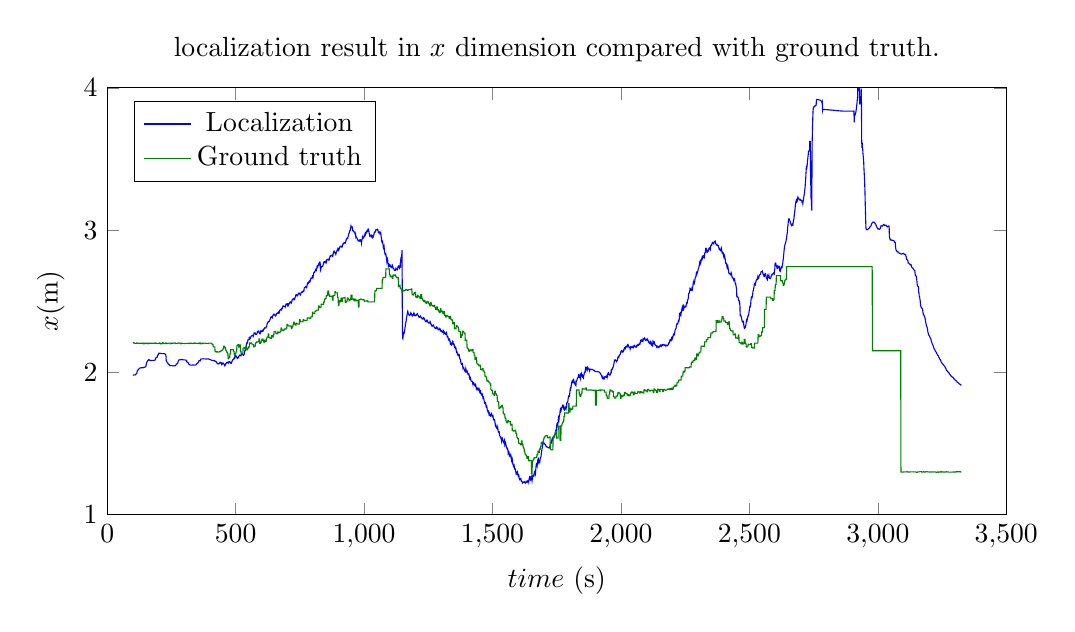
\begin{tikzpicture}

\begin{axis}[
title={localization result in $x$ dimension compared with ground truth.},
xlabel={$time$ (s)},
ylabel={$x$(m)},
xmin=0, xmax=3500,
ymin=1, ymax=4,
axis on top,
width=13cm,
height=7cm,
legend style={at={(0.03,0.97)}, anchor=north west},
legend entries={{Localization},{Ground truth}}
]
\addplot [blue]
coordinates {
(100,1.98128997388918)
(101,1.98079197434912)
(102,1.98134660863179)
(103,1.98106858529597)
(104,1.98143487069458)
(105,1.98187361482629)
(106,1.98182154781867)
(107,1.9814100258086)
(108,1.98126526982431)
(109,1.98145246498364)
(110,1.9824159885013)
(111,1.98716825064075)
(112,1.98759394068925)
(113,1.98846818404825)
(114,1.98972214059645)
(115,1.99056463548323)
(116,2.00018766759502)
(117,2.00745769069534)
(118,2.01302006491927)
(119,2.01442438058576)
(120,2.01597347661818)
(121,2.01743844042286)
(122,2.02161087239335)
(123,2.02255568520725)
(124,2.02439575647651)
(125,2.02570065376345)
(126,2.02815378212179)
(127,2.0289650833035)
(128,2.02961609957816)
(129,2.03126150007311)
(130,2.03137530238683)
(131,2.03151627499619)
(132,2.03174853420449)
(133,2.03201657322614)
(134,2.03202691452833)
(135,2.03183609051121)
(136,2.03182992435916)
(137,2.03177202696757)
(138,2.03180150364224)
(139,2.0318559695907)
(140,2.03182167843091)
(141,2.03400132224782)
(142,2.03404296388825)
(143,2.0341698899379)
(144,2.03582433729796)
(145,2.03574434065096)
(146,2.03599943943846)
(147,2.03674125623337)
(148,2.03706163881898)
(149,2.03893502730262)
(150,2.041428912301)
(151,2.0427054473173)
(152,2.05372578442937)
(153,2.06283261937472)
(154,2.0681410968136)
(155,2.07338091512944)
(156,2.0774033655214)
(157,2.07984999107645)
(158,2.08227247251429)
(159,2.08286547831879)
(160,2.08687949772482)
(161,2.08876851115349)
(162,2.08961774420202)
(163,2.08960844779162)
(164,2.08604514002189)
(165,2.0853973052709)
(166,2.08383067329658)
(167,2.08355692814877)
(168,2.08303502016479)
(169,2.08301443901342)
(170,2.08275986105936)
(171,2.0830449168053)
(172,2.08311507387581)
(173,2.08325124071534)
(174,2.08311316281415)
(175,2.0833166055923)
(176,2.0835322967715)
(177,2.08391725334441)
(178,2.08400354054046)
(179,2.08349777602732)
(180,2.08342840481392)
(181,2.08430977665194)
(182,2.08425668394145)
(183,2.08445411206692)
(184,2.08520220248559)
(185,2.08539634288377)
(186,2.0860545043131)
(187,2.08656422326889)
(188,2.09336759857066)
(189,2.09707124604349)
(190,2.10337113995389)
(191,2.10355963819082)
(192,2.10432154526285)
(193,2.10493296032394)
(194,2.10616594621417)
(195,2.1071324469477)
(196,2.12061587595918)
(197,2.12139576834376)
(198,2.12192149160946)
(199,2.12258239719878)
(200,2.12699043038513)
(201,2.13389722846115)
(202,2.1341511740201)
(203,2.13392007557634)
(204,2.13389065503306)
(205,2.1338268046905)
(206,2.13402841437505)
(207,2.13368752560902)
(208,2.13335744090697)
(209,2.133275988851)
(210,2.13204450700501)
(211,2.13143511548206)
(212,2.13155114326717)
(213,2.13168952731994)
(214,2.1317867759188)
(215,2.13162794777381)
(216,2.13160302440333)
(217,2.13160368663333)
(218,2.13155963148151)
(219,2.13162251319872)
(220,2.13168685382169)
(221,2.13165821843106)
(222,2.13159164929279)
(223,2.13134597762519)
(224,2.13118214135489)
(225,2.12746568562927)
(226,2.12633149933788)
(227,2.12453352960479)
(228,2.12284983858506)
(229,2.11211813182339)
(230,2.08124424377867)
(231,2.07898505115718)
(232,2.07408095368448)
(233,2.0712830607689)
(234,2.06737812558094)
(235,2.06696678393281)
(236,2.06549084715429)
(237,2.06143074955272)
(238,2.05739777744025)
(239,2.0563109832784)
(240,2.05497416473239)
(241,2.05478751415579)
(242,2.05405162350719)
(243,2.0530101729832)
(244,2.04639325094522)
(245,2.04619201624365)
(246,2.04659954660388)
(247,2.04665455189973)
(248,2.04672704118737)
(249,2.04685033342478)
(250,2.04673093068203)
(251,2.04680747970825)
(252,2.0465078301277)
(253,2.04586686561591)
(254,2.04558547411502)
(255,2.04564505199085)
(256,2.04548751667528)
(257,2.04520885060314)
(258,2.0452689241541)
(259,2.04566596809392)
(260,2.04607186225326)
(261,2.0460556428703)
(262,2.04624087449048)
(263,2.04633245560108)
(264,2.04628841459172)
(265,2.04640768264912)
(266,2.0476555894411)
(267,2.04913565176347)
(268,2.05222083844013)
(269,2.05603945918082)
(270,2.05930527290948)
(271,2.05973090852531)
(272,2.0600774498844)
(273,2.06213301122192)
(274,2.06256227132042)
(275,2.06728331946601)
(276,2.07451972350087)
(277,2.08006603430555)
(278,2.08448901018377)
(279,2.08679696359889)
(280,2.08750485305873)
(281,2.08777642094057)
(282,2.08787961670927)
(283,2.08789809137197)
(284,2.08807131600847)
(285,2.08826370626132)
(286,2.09038432449282)
(287,2.09032209228427)
(288,2.09005202429197)
(289,2.09071326624666)
(290,2.09101186957139)
(291,2.0911579481941)
(292,2.09104588536422)
(293,2.08843341630553)
(294,2.08831115962471)
(295,2.08813115531396)
(296,2.0878950100641)
(297,2.08774774313343)
(298,2.0877861787388)
(299,2.08736495802138)
(300,2.08729460880121)
(301,2.08735786207241)
(302,2.08740687361662)
(303,2.08727681106392)
(304,2.08635741732372)
(305,2.08590758047567)
(306,2.08528301981049)
(307,2.08463496764504)
(308,2.0836837106169)
(309,2.08234736521925)
(310,2.0730070564069)
(311,2.07173448463882)
(312,2.06984334961983)
(313,2.06911053352388)
(314,2.06869556863438)
(315,2.06745076690977)
(316,2.06581787270931)
(317,2.06260931305795)
(318,2.05609151380332)
(319,2.05581154683261)
(320,2.05462833095422)
(321,2.05280803335783)
(322,2.0512632072004)
(323,2.05105707703992)
(324,2.05105446847586)
(325,2.05058149792651)
(326,2.05056441860899)
(327,2.05082887047959)
(328,2.05067190476302)
(329,2.05058237232438)
(330,2.050784431735)
(331,2.05087976287762)
(332,2.05131290320006)
(333,2.05149275427046)
(334,2.05135156466209)
(335,2.0511228721656)
(336,2.05113913300728)
(337,2.05120281393969)
(338,2.05070664327223)
(339,2.05070366465477)
(340,2.05054287663505)
(341,2.05050369002703)
(342,2.05055730853684)
(343,2.05057192128012)
(344,2.05157377413618)
(345,2.05187311911335)
(346,2.05218637897726)
(347,2.05433276819083)
(348,2.05864954777293)
(349,2.06097818010683)
(350,2.0614910977577)
(351,2.06214751032608)
(352,2.06435126585848)
(353,2.06619456064176)
(354,2.06890834691368)
(355,2.07116655842988)
(356,2.0756636706337)
(357,2.08055862113213)
(358,2.08105896146488)
(359,2.08137523588598)
(360,2.08162224572668)
(361,2.08150283515192)
(362,2.08141055645514)
(363,2.08150204505735)
(364,2.09219958245941)
(365,2.09326155587109)
(366,2.09419868889989)
(367,2.09408699060257)
(368,2.09409110712892)
(369,2.09409995973869)
(370,2.09404746275524)
(371,2.09405123886582)
(372,2.09472940268823)
(373,2.09470826398624)
(374,2.09492581375668)
(375,2.09490213786197)
(376,2.09457670749845)
(377,2.09437072912367)
(378,2.09425744725617)
(379,2.09422314182691)
(380,2.09424294587607)
(381,2.0942359439345)
(382,2.09425920931393)
(383,2.09418859266782)
(384,2.09415249458829)
(385,2.0926766195898)
(386,2.09245699797354)
(387,2.09242119338999)
(388,2.09339117117514)
(389,2.09392089455684)
(390,2.09414154192077)
(391,2.09402172029964)
(392,2.09393525246017)
(393,2.09380897083619)
(394,2.09376809435436)
(395,2.09363281958866)
(396,2.09326257934319)
(397,2.09261413655409)
(398,2.09192448240001)
(399,2.0912333162397)
(400,2.08997113681422)
(401,2.08894458606345)
(402,2.08847545231583)
(403,2.08751326117317)
(404,2.08688800460505)
(405,2.08594248574587)
(406,2.08523535794941)
(407,2.08453358927348)
(408,2.08442784558177)
(409,2.08421984756761)
(410,2.08415788983694)
(411,2.08310142578632)
(412,2.0830820864775)
(413,2.08296632220787)
(414,2.08242487900445)
(415,2.08186535035529)
(416,2.08106571742551)
(417,2.08077167208887)
(418,2.08135943737523)
(419,2.08113694194228)
(420,2.07993083018747)
(421,2.07622054201699)
(422,2.07568819804693)
(423,2.07511576587103)
(424,2.07506711546262)
(425,2.07445104851334)
(426,2.06737133106704)
(427,2.06676841688901)
(428,2.06505720113969)
(429,2.06343130361946)
(430,2.05941260148905)
(431,2.05960158186583)
(432,2.05944969493136)
(433,2.06014981799821)
(434,2.06036448738193)
(435,2.05943253450541)
(436,2.06192740255181)
(437,2.06385878436789)
(438,2.06708316389806)
(439,2.07051563474385)
(440,2.07135142090957)
(441,2.07028390757272)
(442,2.06524433794064)
(443,2.06405140253229)
(444,2.06562358733851)
(445,2.05837017937808)
(446,2.05311233908103)
(447,2.05481609043126)
(448,2.06038313281315)
(449,2.06464083103344)
(450,2.06370033042149)
(451,2.06243324523646)
(452,2.06477213832548)
(453,2.0632349725931)
(454,2.05828319372866)
(455,2.05747746904303)
(456,2.05561742626374)
(457,2.0500864464996)
(458,2.04638928532575)
(459,2.0498941283055)
(460,2.0514094797735)
(461,2.05946639703426)
(462,2.06177362265953)
(463,2.06110649228675)
(464,2.06660167877267)
(465,2.06891107015565)
(466,2.07006479462305)
(467,2.06908280791462)
(468,2.06846628276462)
(469,2.07028601617839)
(470,2.06601062117022)
(471,2.06370385257734)
(472,2.06634049652551)
(473,2.07071453515697)
(474,2.07325113634599)
(475,2.07118726349793)
(476,2.07206418166474)
(477,2.07472210483394)
(478,2.07348275130016)
(479,2.0703525026294)
(480,2.06799476582855)
(481,2.06403305290742)
(482,2.06187701682154)
(483,2.06302759308137)
(484,2.06568292949711)
(485,2.0727811277054)
(486,2.07956309784771)
(487,2.0798003604763)
(488,2.08284033543381)
(489,2.08815847916589)
(490,2.0913930066209)
(491,2.09204770045068)
(492,2.09195161146864)
(493,2.09488578390046)
(494,2.10000081412748)
(495,2.0963637385819)
(496,2.09714124011341)
(497,2.1016050353859)
(498,2.11156846409458)
(499,2.11613318977282)
(500,2.11522641537656)
(501,2.11649460681839)
(502,2.11479629962797)
(503,2.11020641205819)
(504,2.10614406993617)
(505,2.10211350680953)
(506,2.09898305531074)
(507,2.09900995667481)
(508,2.09763704629763)
(509,2.09950607558054)
(510,2.1046660498636)
(511,2.10818221154461)
(512,2.1072140781205)
(513,2.11155056539769)
(514,2.11905605385672)
(515,2.12091168827058)
(516,2.12002016244789)
(517,2.11986183594907)
(518,2.12143519731147)
(519,2.12088326310677)
(520,2.11577058446899)
(521,2.11611453478702)
(522,2.12335107891977)
(523,2.12499307795898)
(524,2.12508659129464)
(525,2.12642285665863)
(526,2.12838983096246)
(527,2.12546746860988)
(528,2.12226512254804)
(529,2.12147067948165)
(530,2.11978389095947)
(531,2.11926810774661)
(532,2.12160859321475)
(533,2.12590632474113)
(534,2.1330908466296)
(535,2.14922835124155)
(536,2.15050544171787)
(537,2.15118451023327)
(538,2.15708680274606)
(539,2.16047039489644)
(540,2.1645086085818)
(541,2.18714039397736)
(542,2.19572926538094)
(543,2.20417298424669)
(544,2.20734905857671)
(545,2.20498208176147)
(546,2.21019473551616)
(547,2.21845484561654)
(548,2.22781791835566)
(549,2.22818342300768)
(550,2.22790356454678)
(551,2.23033998564143)
(552,2.23105684129592)
(553,2.24485154211425)
(554,2.24639012633827)
(555,2.2457287869644)
(556,2.23686392522281)
(557,2.24000272434771)
(558,2.24510273453073)
(559,2.2481030264923)
(560,2.25477503266604)
(561,2.25519029590613)
(562,2.25549301105705)
(563,2.25519078349019)
(564,2.25712620017046)
(565,2.25863939101974)
(566,2.25937244204553)
(567,2.2603868223203)
(568,2.26008645943097)
(569,2.25488936882839)
(570,2.26104377315636)
(571,2.26705202048779)
(572,2.27549869222612)
(573,2.27323630354788)
(574,2.27232352333681)
(575,2.27294808628577)
(576,2.27585977423341)
(577,2.27055831296866)
(578,2.26707019803692)
(579,2.26664849800405)
(580,2.26720667901341)
(581,2.26867023943396)
(582,2.26823429335332)
(583,2.27084001034787)
(584,2.27805977184774)
(585,2.28733210702329)
(586,2.2885218413066)
(587,2.28760077674735)
(588,2.28697140586258)
(589,2.28974556871285)
(590,2.28857492500801)
(591,2.27977740909715)
(592,2.27975088964709)
(593,2.27883399632216)
(594,2.27139616645892)
(595,2.27019508541237)
(596,2.2745334279863)
(597,2.28750777740019)
(598,2.29166257500039)
(599,2.28947822935672)
(600,2.28706584726593)
(601,2.29144364766693)
(602,2.29128159292739)
(603,2.28980016029651)
(604,2.29409411247628)
(605,2.29207105962118)
(606,2.28902946633832)
(607,2.29107812924786)
(608,2.29529799883506)
(609,2.30009020919147)
(610,2.30547870386201)
(611,2.3047718587236)
(612,2.30703295829657)
(613,2.3129925712099)
(614,2.31318604869714)
(615,2.31232219476419)
(616,2.31114629994402)
(617,2.3123479664399)
(618,2.31193609738005)
(619,2.3202788809266)
(620,2.32079094551387)
(621,2.32334115334054)
(622,2.33469569987095)
(623,2.34121727003084)
(624,2.3439493308665)
(625,2.34863716991217)
(626,2.35386609709763)
(627,2.35424359334293)
(628,2.35395488009023)
(629,2.35842819914863)
(630,2.35984691514468)
(631,2.35916359790161)
(632,2.36095272297578)
(633,2.36500057009846)
(634,2.37299495561938)
(635,2.37630626483446)
(636,2.37752611722238)
(637,2.38632816172387)
(638,2.38976280985805)
(639,2.38826993002837)
(640,2.38735253209892)
(641,2.38908864064893)
(642,2.39129104973969)
(643,2.38546290410988)
(644,2.39029937976663)
(645,2.39589592973025)
(646,2.40167840096234)
(647,2.40575724746684)
(648,2.40410561871669)
(649,2.40401687132484)
(650,2.4074799229009)
(651,2.40799636911993)
(652,2.40487435468666)
(653,2.40150840569013)
(654,2.4018109347627)
(655,2.39717874957072)
(656,2.39571270445678)
(657,2.39844254669348)
(658,2.40610452229943)
(659,2.41239763187565)
(660,2.41299530524175)
(661,2.41429399470809)
(662,2.4143505692426)
(663,2.41741284529023)
(664,2.41562959062531)
(665,2.4144482542738)
(666,2.4156143585114)
(667,2.42027400366748)
(668,2.41554084883911)
(669,2.41550777558965)
(670,2.42016623281453)
(671,2.43198193007582)
(672,2.43701274916021)
(673,2.43692398203626)
(674,2.43963824338929)
(675,2.43799610672342)
(676,2.43703270606955)
(677,2.43705513668333)
(678,2.44433353661554)
(679,2.44141800054332)
(680,2.44565888187434)
(681,2.44778715972556)
(682,2.45229779159259)
(683,2.4566251635229)
(684,2.46374812199485)
(685,2.46244184701687)
(686,2.46378936849072)
(687,2.46646685035719)
(688,2.46507258922427)
(689,2.46370098041658)
(690,2.4619433836852)
(691,2.46387738812843)
(692,2.46242312726836)
(693,2.4588944003096)
(694,2.46508706620907)
(695,2.47053554929424)
(696,2.47884561935791)
(697,2.47863331550164)
(698,2.47816265158003)
(699,2.48021997066423)
(700,2.4772676946764)
(701,2.47923110874738)
(702,2.47331075743668)
(703,2.47607923420838)
(704,2.46683833319813)
(705,2.46987201775737)
(706,2.47520445774439)
(707,2.48152815796504)
(708,2.48255028822846)
(709,2.48197538778423)
(710,2.4839568170379)
(711,2.4914533970993)
(712,2.49415405593563)
(713,2.49180012262788)
(714,2.49239059400049)
(715,2.49408739247512)
(716,2.49423775481604)
(717,2.48827563919591)
(718,2.49197850770875)
(719,2.49861709876657)
(720,2.51023984310116)
(721,2.51113574283516)
(722,2.51151577614423)
(723,2.51621039481748)
(724,2.51792179070036)
(725,2.51654296900057)
(726,2.51948280948656)
(727,2.5197700803561)
(728,2.51012111390928)
(729,2.51028625762812)
(730,2.51507762674421)
(731,2.52200418627311)
(732,2.52951895722908)
(733,2.5298705480576)
(734,2.54178332606566)
(735,2.54511432430286)
(736,2.54614806245945)
(737,2.54555076130148)
(738,2.54518445755672)
(739,2.54250793019528)
(740,2.53745487039817)
(741,2.53885208648611)
(742,2.54131847086154)
(743,2.5480114303394)
(744,2.5535809809139)
(745,2.5520023387873)
(746,2.55311187888449)
(747,2.55622818121906)
(748,2.55257453779284)
(749,2.55210474253011)
(750,2.55199915724035)
(751,2.54747313570219)
(752,2.54330811722365)
(753,2.54477753871522)
(754,2.55433936760926)
(755,2.56119084466839)
(756,2.56232321449898)
(757,2.56300930439852)
(758,2.56252931266947)
(759,2.56611068687756)
(760,2.56486562914882)
(761,2.56897854514207)
(762,2.57104535438979)
(763,2.57225054976936)
(764,2.57164571209057)
(765,2.56927065207717)
(766,2.57379341809205)
(767,2.59204140966985)
(768,2.59530329114507)
(769,2.59485922767788)
(770,2.59595531028883)
(771,2.60077280622893)
(772,2.60117728054894)
(773,2.60102615241758)
(774,2.60424140178709)
(775,2.60234471764579)
(776,2.59633401756984)
(777,2.5994470919191)
(778,2.6065400798317)
(779,2.62125766364406)
(780,2.62701907213632)
(781,2.62938267192901)
(782,2.62942364415285)
(783,2.62693841606937)
(784,2.63267463794489)
(785,2.63513823729154)
(786,2.63844104774974)
(787,2.64267010519594)
(788,2.64215713326932)
(789,2.63580464895778)
(790,2.63967457525622)
(791,2.64793334521827)
(792,2.65504484253656)
(793,2.66116401980645)
(794,2.66103279609789)
(795,2.66092817133011)
(796,2.66291620012575)
(797,2.66392939414663)
(798,2.66928456106463)
(799,2.67450110024625)
(800,2.67038488492294)
(801,2.66487067026859)
(802,2.67455614397362)
(803,2.6824197561192)
(804,2.6978805009557)
(805,2.70344545232797)
(806,2.70438162633439)
(807,2.70534737644748)
(808,2.70396044915974)
(809,2.71083521725033)
(810,2.71527083326636)
(811,2.71773502600373)
(812,2.72206997367034)
(813,2.71712865691384)
(814,2.71525025834432)
(815,2.7218472910771)
(816,2.73172624200796)
(817,2.74539041734886)
(818,2.74844228781517)
(819,2.74744855981985)
(820,2.74363402684746)
(821,2.74995594248651)
(822,2.75603004651177)
(823,2.75987192539793)
(824,2.76359799394683)
(825,2.76728878902428)
(826,2.75658599755933)
(827,2.75788321375521)
(828,2.76448519870871)
(829,2.77785193656764)
(830,2.71587359520266)
(831,2.72121196643917)
(832,2.72802601944087)
(833,2.73470271594641)
(834,2.73983043023159)
(835,2.74435762037565)
(836,2.74433713172137)
(837,2.74514964160072)
(838,2.74444894470473)
(839,2.7450062922842)
(840,2.75096196699978)
(841,2.7590299511861)
(842,2.77011496170204)
(843,2.77419387421471)
(844,2.77290128801691)
(845,2.77182501154235)
(846,2.77756727166474)
(847,2.7771411671687)
(848,2.77823417758406)
(849,2.77782438642026)
(850,2.77978896575945)
(851,2.7700839974668)
(852,2.76728311781372)
(853,2.77132559632549)
(854,2.78344508043944)
(855,2.79009429833724)
(856,2.78900252563292)
(857,2.79108584952907)
(858,2.79374150513653)
(859,2.79449566832253)
(860,2.79602401362929)
(861,2.79555750676042)
(862,2.79422737185858)
(863,2.78869644401721)
(864,2.78929403982162)
(865,2.7934803829688)
(866,2.80435997996101)
(867,2.8133801608464)
(868,2.81686635910098)
(869,2.81572191798372)
(870,2.81642204495505)
(871,2.82036351631712)
(872,2.82135961120194)
(873,2.82169166774545)
(874,2.82370270493609)
(875,2.82416404582654)
(876,2.81838064928473)
(877,2.81465710582791)
(878,2.81588914284843)
(879,2.82360972185253)
(880,2.83774947998999)
(881,2.84003296942237)
(882,2.85106988001256)
(883,2.85267341629237)
(884,2.84775180967923)
(885,2.84654557171044)
(886,2.84436790427499)
(887,2.83809155042106)
(888,2.83404186449254)
(889,2.83454261545939)
(890,2.82944366771773)
(891,2.8365712095384)
(892,2.84590219308814)
(893,2.85139497717709)
(894,2.85129734043204)
(895,2.8557866316668)
(896,2.86150442181955)
(897,2.86093745110953)
(898,2.87000242438275)
(899,2.86686195467482)
(900,2.86179934340349)
(901,2.85733416654609)
(902,2.86102942131625)
(903,2.8669554381041)
(904,2.87589492849619)
(905,2.88128226149482)
(906,2.88088512488491)
(907,2.88081796057945)
(908,2.88363117123539)
(909,2.8858905680854)
(910,2.88464206765962)
(911,2.88764759318872)
(912,2.88738757059059)
(913,2.88366111799067)
(914,2.88060299062981)
(915,2.88314657560916)
(916,2.88994629511282)
(917,2.89749588798119)
(918,2.9042834899637)
(919,2.90370898149564)
(920,2.90383063012444)
(921,2.90790716146121)
(922,2.91226515448714)
(923,2.91190954711734)
(924,2.91077962056869)
(925,2.91161481009984)
(926,2.90751363007172)
(927,2.90775398379668)
(928,2.91045157478674)
(929,2.92121703481766)
(930,2.92979700862405)
(931,2.93593540155379)
(932,2.93423494825818)
(933,2.93663834689709)
(934,2.9384334280747)
(935,2.94593177407416)
(936,2.94727034773513)
(937,2.94618895595326)
(938,2.95573161238193)
(939,2.96186652818644)
(940,2.97031422154396)
(941,2.97737136854036)
(942,2.97880131430904)
(943,2.98547522224437)
(944,2.99551875638507)
(945,2.99851325651071)
(946,2.99808244653721)
(947,3.01197687914499)
(948,3.01040461983031)
(949,3.02873726411158)
(950,3.02349006851817)
(951,3.02278854525624)
(952,3.02371154289467)
(953,3.02396868018803)
(954,3.02004158362846)
(955,3.01251896238768)
(956,2.99679842220186)
(957,2.99448966547513)
(958,2.99556868347332)
(959,2.99139249775763)
(960,2.99022272997307)
(961,2.98592552472235)
(962,2.98591495802987)
(963,2.98352728391469)
(964,2.98446620315301)
(965,2.97322522245443)
(966,2.97441601255658)
(967,2.97572710931203)
(968,2.95044417732819)
(969,2.9534311134071)
(970,2.94802215680979)
(971,2.94529702979675)
(972,2.94472442398422)
(973,2.94157966758117)
(974,2.93531519677213)
(975,2.93170075590351)
(976,2.92838099486476)
(977,2.92419951125587)
(978,2.92367749598697)
(979,2.92519270510671)
(980,2.9233939740993)
(981,2.92851917093836)
(982,2.92705894655538)
(983,2.92766325297723)
(984,2.92489631139133)
(985,2.93250321149495)
(986,2.93164799781444)
(987,2.92856493926703)
(988,2.92611326198931)
(989,2.92234033477199)
(990,2.90917300272331)
(991,2.92470778375387)
(992,2.93438645010243)
(993,2.93785091379316)
(994,2.94928682092634)
(995,2.94186820256538)
(996,2.94161043736306)
(997,2.94437089180949)
(998,2.95043381363983)
(999,2.95380661743435)
(1000,2.95764916198363)
(1001,2.95558711885694)
(1002,2.95461163174433)
(1003,2.96955945170072)
(1004,2.9774308135149)
(1005,2.9804432737782)
(1006,2.97133275575411)
(1007,2.97562735887068)
(1008,2.97867271556919)
(1009,2.9814688927385)
(1010,2.98622956252869)
(1011,2.99520276579572)
(1012,2.99829686935905)
(1013,2.9984744532699)
(1014,2.99473768648548)
(1015,3.00133233268155)
(1016,3.00806401531676)
(1017,3.00734211345282)
(1018,2.99828661248507)
(1019,2.99079404941395)
(1020,2.97796078783583)
(1021,2.96693376123982)
(1022,2.96080403983393)
(1023,2.96415134621111)
(1024,2.96024925478479)
(1025,2.96076347085514)
(1026,2.95769007010129)
(1027,2.954035562792)
(1028,2.96279854438473)
(1029,2.96487733901884)
(1030,2.96361902242545)
(1031,2.96090514958893)
(1032,2.95540750343155)
(1033,2.94841072070701)
(1034,2.94509873798004)
(1035,2.94715146788355)
(1036,2.95982299511852)
(1037,2.96421461659164)
(1038,2.96570303932781)
(1039,2.97343839400731)
(1040,2.98496181005419)
(1041,2.98619566414835)
(1042,2.98393034270522)
(1043,2.98655697062759)
(1044,2.98739677009005)
(1045,2.99396219713072)
(1046,3.00199257187102)
(1047,3.00023172285591)
(1048,3.00157831752587)
(1049,3.00453156127325)
(1050,3.00394159232889)
(1051,3.00205485392876)
(1052,3.0063566993372)
(1053,3.00612353731789)
(1054,3.00046242529157)
(1055,2.98936596038268)
(1056,2.98161349475291)
(1057,2.98315742134706)
(1058,2.98363411674829)
(1059,2.98609137748921)
(1060,2.98677095227826)
(1061,2.97940086417)
(1062,2.97241142358694)
(1063,2.97290502336849)
(1064,2.97193934373745)
(1065,2.97861024046343)
(1066,2.96377126956686)
(1067,2.947088380784)
(1068,2.93441229338296)
(1069,2.9196649843535)
(1070,2.91209781823471)
(1071,2.91327782287625)
(1072,2.91808811512415)
(1073,2.91144099072964)
(1074,2.89299898314693)
(1075,2.87799804938809)
(1076,2.87142787945935)
(1077,2.87411355429583)
(1078,2.88203527609937)
(1079,2.86276185968889)
(1080,2.84411783351561)
(1081,2.8350605410212)
(1082,2.82986468917028)
(1083,2.82530063954518)
(1084,2.82484942023441)
(1085,2.82932830728633)
(1086,2.81702379323088)
(1087,2.80423581428459)
(1088,2.7880396608927)
(1089,2.77469990558129)
(1090,2.78208228652849)
(1091,2.79416647698544)
(1092,2.78594247665899)
(1093,2.76837254699438)
(1094,2.76621128560937)
(1095,2.74230340917334)
(1096,2.74373261818947)
(1097,2.74786390736299)
(1098,2.7573574462225)
(1099,2.75494767497399)
(1100,2.74492584987417)
(1101,2.74385567621652)
(1102,2.74506148532776)
(1103,2.75323096356233)
(1104,2.75407976652743)
(1105,2.74259471197521)
(1106,2.73746105086029)
(1107,2.73660379223364)
(1108,2.74330601843556)
(1109,2.74314616439494)
(1110,2.7451598610857)
(1111,2.7504505483993)
(1112,2.74220983887422)
(1113,2.7315649706646)
(1114,2.72834659642036)
(1115,2.72851041590089)
(1116,2.72733629274312)
(1117,2.72218659476064)
(1118,2.71727459833637)
(1119,2.71730531314003)
(1120,2.71836479064623)
(1121,2.71903478930908)
(1122,2.71783615198237)
(1123,2.72473035697598)
(1124,2.73131161919431)
(1125,2.72915986814248)
(1126,2.72808567062537)
(1127,2.72504832554386)
(1128,2.72449797092531)
(1129,2.72057053869634)
(1130,2.72483252883428)
(1131,2.73330734263818)
(1132,2.73929194021868)
(1133,2.74547748130663)
(1134,2.74743060586751)
(1135,2.74439591945757)
(1136,2.74017377451234)
(1137,2.7422656272616)
(1138,2.73352592098064)
(1139,2.73777151570311)
(1140,2.7520118398776)
(1141,2.74267780770385)
(1142,2.74127657699118)
(1143,2.79428119444022)
(1144,2.7892508266376)
(1145,2.79575334543006)
(1146,2.80994828498117)
(1147,2.83261022948154)
(1148,2.85876718256031)
(1149,2.36917940976492)
(1150,2.2420549726914)
(1151,2.23723027774884)
(1152,2.25184302481222)
(1153,2.27490149678374)
(1154,2.2713475833665)
(1155,2.27130160227341)
(1156,2.2736161435321)
(1157,2.28396933033672)
(1158,2.29339379753244)
(1159,2.30883201124774)
(1160,2.32048008810464)
(1161,2.33345038334952)
(1162,2.34332448989135)
(1163,2.35428940342503)
(1164,2.36479294222489)
(1165,2.37398837882906)
(1166,2.3884088608118)
(1167,2.39790820250889)
(1168,2.41042272887092)
(1169,2.4231031575443)
(1170,2.42921283273193)
(1171,2.42407798590341)
(1172,2.41180150953651)
(1173,2.41010413503162)
(1174,2.40648385188137)
(1175,2.40510617130039)
(1176,2.39897501675656)
(1177,2.39904152459045)
(1178,2.39964192397222)
(1179,2.40438059068733)
(1180,2.40621766352792)
(1181,2.41336803499813)
(1182,2.4182105667732)
(1183,2.4143270239917)
(1184,2.41068648323661)
(1185,2.40434897811962)
(1186,2.40503604832076)
(1187,2.40484347368756)
(1188,2.39829503813547)
(1189,2.40145140819855)
(1190,2.40237300890911)
(1191,2.40482439021441)
(1192,2.40364233335866)
(1193,2.41250273278651)
(1194,2.41767285867249)
(1195,2.41448874415204)
(1196,2.40712256991927)
(1197,2.4011627166912)
(1198,2.40289546113063)
(1199,2.4018015193847)
(1200,2.39757939861965)
(1201,2.39718638023474)
(1202,2.39779906584805)
(1203,2.40368939721987)
(1204,2.4051172697263)
(1205,2.4075538962473)
(1206,2.4111879288713)
(1207,2.41307173406578)
(1208,2.40994018345027)
(1209,2.40448552364325)
(1210,2.40047439092871)
(1211,2.398857070562)
(1212,2.39808807882071)
(1213,2.39134519595188)
(1214,2.38720232972479)
(1215,2.38756616583696)
(1216,2.38939458751379)
(1217,2.3881814688032)
(1218,2.39092788241654)
(1219,2.39539449947831)
(1220,2.39292873153949)
(1221,2.39082504541903)
(1222,2.385963725752)
(1223,2.3826188069464)
(1224,2.38334871150426)
(1225,2.38272024773217)
(1226,2.37615244086959)
(1227,2.37593346577871)
(1228,2.37479633276846)
(1229,2.37724783959678)
(1230,2.37611950097498)
(1231,2.37868477649196)
(1232,2.38425522709426)
(1233,2.38260108520954)
(1234,2.37929392862814)
(1235,2.37242165988179)
(1236,2.36909660811404)
(1237,2.36795792158197)
(1238,2.36361997344761)
(1239,2.35828213226958)
(1240,2.35608521538919)
(1241,2.35665940437359)
(1242,2.35592348665066)
(1243,2.35559517254718)
(1244,2.36471393987066)
(1245,2.36729500190812)
(1246,2.36273823564459)
(1247,2.35503946493113)
(1248,2.35369902423971)
(1249,2.3540860272393)
(1250,2.35051067872121)
(1251,2.34841463730898)
(1252,2.3461560051488)
(1253,2.3457731899944)
(1254,2.34689679610535)
(1255,2.34685556536657)
(1256,2.35127609400994)
(1257,2.35635017653749)
(1258,2.35254325492816)
(1259,2.34751629108394)
(1260,2.33896102368759)
(1261,2.33640646966376)
(1262,2.33665676629823)
(1263,2.33167726242983)
(1264,2.32581275824985)
(1265,2.32342604461899)
(1266,2.32563343169347)
(1267,2.3271305526989)
(1268,2.32869185895026)
(1269,2.33244706706074)
(1270,2.33271457934099)
(1271,2.32872054768413)
(1272,2.32125179328702)
(1273,2.31821388811489)
(1274,2.31609740496656)
(1275,2.31292602806069)
(1276,2.3108989249274)
(1277,2.30864805814638)
(1278,2.30708312563676)
(1279,2.30883430954163)
(1280,2.30826697792281)
(1281,2.31345954934551)
(1282,2.3196704229663)
(1283,2.3194567788518)
(1284,2.31362893231351)
(1285,2.30759400420124)
(1286,2.30595650433764)
(1287,2.30940758429312)
(1288,2.30613800164492)
(1289,2.30147218690122)
(1290,2.29902225519826)
(1291,2.30003352556971)
(1292,2.30082910365613)
(1293,2.2998102946092)
(1294,2.3043428479589)
(1295,2.30828890978032)
(1296,2.30474486627772)
(1297,2.30026451437854)
(1298,2.29246924270723)
(1299,2.29386863289356)
(1300,2.2937364173335)
(1301,2.29128200657388)
(1302,2.28786454912709)
(1303,2.28336510345593)
(1304,2.28325334726743)
(1305,2.28413772764623)
(1306,2.28181157677116)
(1307,2.28772417936945)
(1308,2.29470664589619)
(1309,2.2926066854299)
(1310,2.28275911444529)
(1311,2.27174047782966)
(1312,2.27495006664119)
(1313,2.27983747187009)
(1314,2.28152252954891)
(1315,2.27684659098652)
(1316,2.2719137507514)
(1317,2.26895485485556)
(1318,2.26710230125127)
(1319,2.26767296485644)
(1320,2.27161421187536)
(1321,2.2766293438782)
(1322,2.26905640198946)
(1323,2.25434765695515)
(1324,2.24820361615839)
(1325,2.24889922343035)
(1326,2.25000422298454)
(1327,2.24687945073982)
(1328,2.23441085080475)
(1329,2.23037517773724)
(1330,2.22614914793488)
(1331,2.22321383390905)
(1332,2.22261563339887)
(1333,2.22896898180075)
(1334,2.22376192718335)
(1335,2.21222632052914)
(1336,2.19768928924932)
(1337,2.19819077135542)
(1338,2.20316287918269)
(1339,2.1949880064962)
(1340,2.1911434892665)
(1341,2.19251662915739)
(1342,2.19941296338071)
(1343,2.20275682286561)
(1344,2.20697726014914)
(1345,2.21741957477151)
(1346,2.21564722174401)
(1347,2.2028717684868)
(1348,2.19546407733804)
(1349,2.19361321790586)
(1350,2.19683114921052)
(1351,2.19229464441349)
(1352,2.18114569585366)
(1353,2.17318643937581)
(1354,2.17350820732106)
(1355,2.17101767416308)
(1356,2.16738022077349)
(1357,2.17319718502494)
(1358,2.16935167355979)
(1359,2.15151606745368)
(1360,2.13998926474617)
(1361,2.14052041800543)
(1362,2.14193142224627)
(1363,2.13520650019334)
(1364,2.12561212586316)
(1365,2.12116276299032)
(1366,2.11990086777831)
(1367,2.11813521799825)
(1368,2.12319726922756)
(1369,2.12685279345561)
(1370,2.12555122099381)
(1371,2.11522950144991)
(1372,2.10032738869706)
(1373,2.09599852417187)
(1374,2.09133103433925)
(1375,2.09062912110882)
(1376,2.07942602640721)
(1377,2.06594623002728)
(1378,2.05952407360123)
(1379,2.05701771419646)
(1380,2.06241634521812)
(1381,2.06129208019831)
(1382,2.06248040518438)
(1383,2.0559451927702)
(1384,2.04023544667682)
(1385,2.02981939013277)
(1386,2.03422645311198)
(1387,2.03463648362992)
(1388,2.0323176974279)
(1389,2.02533276516239)
(1390,2.01816428253612)
(1391,2.01243733438266)
(1392,2.01099756570818)
(1393,2.00780314595073)
(1394,2.00501438883843)
(1395,2.01281710808832)
(1396,2.02524006116874)
(1397,2.01455574350882)
(1398,2.00464736967002)
(1399,2.00285017046948)
(1400,2.00716784940548)
(1401,2.00998307949486)
(1402,2.00298823568819)
(1403,1.99714355538538)
(1404,1.98939885372517)
(1405,1.98456046630671)
(1406,1.98346583225003)
(1407,1.985360541008)
(1408,1.98788220867288)
(1409,1.98062989308733)
(1410,1.97026357589021)
(1411,1.95233481248453)
(1412,1.95263078565724)
(1413,1.95497265844458)
(1414,1.95986283697945)
(1415,1.95185075135385)
(1416,1.94204575329173)
(1417,1.93910449662241)
(1418,1.93929773638458)
(1419,1.93745247066233)
(1420,1.93614712913759)
(1421,1.93710794708141)
(1422,1.93462330267019)
(1423,1.92134094467197)
(1424,1.91339127752803)
(1425,1.9211701651704)
(1426,1.92657710212718)
(1427,1.92733682543111)
(1428,1.9195360242839)
(1429,1.91590884747427)
(1430,1.91099809525609)
(1431,1.91011031220571)
(1432,1.90506779474221)
(1433,1.9078640402698)
(1434,1.91441419895712)
(1435,1.91151149570828)
(1436,1.89512912311194)
(1437,1.88564036524276)
(1438,1.89121999666246)
(1439,1.89207768556897)
(1440,1.89116497876559)
(1441,1.88459229076406)
(1442,1.8784873362469)
(1443,1.8758836421842)
(1444,1.87488124196149)
(1445,1.87577818457491)
(1446,1.88349274052345)
(1447,1.88776738971372)
(1448,1.88341505321346)
(1449,1.87593216278961)
(1450,1.86156589159955)
(1451,1.85746582938362)
(1452,1.86364387141546)
(1453,1.86643295618309)
(1454,1.85654501238712)
(1455,1.85155744562157)
(1456,1.84458122070737)
(1457,1.84238131824459)
(1458,1.83911422179618)
(1459,1.8392476977442)
(1460,1.8472189951246)
(1461,1.84369182222949)
(1462,1.82835463622568)
(1463,1.81691536728259)
(1464,1.81915388446356)
(1465,1.82178066300215)
(1466,1.81262383525176)
(1467,1.80496778543374)
(1468,1.79469367203187)
(1469,1.78269741876683)
(1470,1.78117415106533)
(1471,1.78683441570159)
(1472,1.78592455281151)
(1473,1.78689617814738)
(1474,1.77198468301803)
(1475,1.75984936481417)
(1476,1.75275125051736)
(1477,1.75139063950285)
(1478,1.75674440384948)
(1479,1.74350345476753)
(1480,1.73110712973223)
(1481,1.72883578004971)
(1482,1.7234080492882)
(1483,1.71881240851312)
(1484,1.72107542636193)
(1485,1.72468004544345)
(1486,1.71315662315821)
(1487,1.69841518574465)
(1488,1.69960602539697)
(1489,1.70514849422459)
(1490,1.69884048879462)
(1491,1.69566408788549)
(1492,1.6924190484155)
(1493,1.69325948890162)
(1494,1.69336538264225)
(1495,1.70271557581006)
(1496,1.71040966831319)
(1497,1.70769973456323)
(1498,1.70085989781383)
(1499,1.69226268037986)
(1500,1.68823216949455)
(1501,1.68675496057427)
(1502,1.69041196386355)
(1503,1.67756693897771)
(1504,1.66605508435279)
(1505,1.66451413342135)
(1506,1.66326460342487)
(1507,1.6630318135788)
(1508,1.66492281624144)
(1509,1.65724220443496)
(1510,1.63938658655134)
(1511,1.62755885224961)
(1512,1.63325416096996)
(1513,1.63047795969833)
(1514,1.62184544538092)
(1515,1.61666772075111)
(1516,1.60901301237591)
(1517,1.60575983679734)
(1518,1.60324989409045)
(1519,1.60497981143112)
(1520,1.61309849198443)
(1521,1.601532490873)
(1522,1.58647451411212)
(1523,1.57920323221651)
(1524,1.57752841577632)
(1525,1.58078746777405)
(1526,1.58179926359051)
(1527,1.56669703332451)
(1528,1.55529133709498)
(1529,1.55068448134769)
(1530,1.54789651178167)
(1531,1.54273362620199)
(1532,1.53909261881889)
(1533,1.54080775957921)
(1534,1.53249207398797)
(1535,1.51695391366672)
(1536,1.526512605138)
(1537,1.53188564364565)
(1538,1.53578471427527)
(1539,1.52942789212434)
(1540,1.52084725052042)
(1541,1.51582027301355)
(1542,1.50990445240823)
(1543,1.50828236050247)
(1544,1.50490366285746)
(1545,1.51334457381897)
(1546,1.52059226587959)
(1547,1.50244937044221)
(1548,1.48732473849349)
(1549,1.49157427802354)
(1550,1.49879198218781)
(1551,1.50430041922492)
(1552,1.49302322768103)
(1553,1.48456022751352)
(1554,1.47548910609122)
(1555,1.46845133253331)
(1556,1.4655863414947)
(1557,1.46252892815075)
(1558,1.46651016885101)
(1559,1.46508416129404)
(1560,1.45290908407077)
(1561,1.43139811753372)
(1562,1.43760462005364)
(1563,1.44198858733791)
(1564,1.43919578533504)
(1565,1.42684945048244)
(1566,1.41891893295039)
(1567,1.41056037439056)
(1568,1.40793685899665)
(1569,1.40988004596504)
(1570,1.41624206774137)
(1571,1.42063845058742)
(1572,1.41109696789792)
(1573,1.39513407776356)
(1574,1.38277523001791)
(1575,1.39271452094659)
(1576,1.39684824531207)
(1577,1.38966138920294)
(1578,1.37753558302135)
(1579,1.35538709956215)
(1580,1.34909433536575)
(1581,1.3434633835028)
(1582,1.33799621258868)
(1583,1.34122033847409)
(1584,1.34562181973216)
(1585,1.3346321405319)
(1586,1.31955436459602)
(1587,1.3188839383864)
(1588,1.32136789291013)
(1589,1.31932036597534)
(1590,1.30492263042304)
(1591,1.29467411180429)
(1592,1.28326811552399)
(1593,1.28460454255236)
(1594,1.28426366208488)
(1595,1.28938406069568)
(1596,1.29864499461157)
(1597,1.30115301792605)
(1598,1.29132901032799)
(1599,1.27848838313436)
(1600,1.2725085313803)
(1601,1.27717242604071)
(1602,1.27836102934262)
(1603,1.26922713994669)
(1604,1.25375536073147)
(1605,1.24962772310508)
(1606,1.24382049619848)
(1607,1.24494758864085)
(1608,1.24864626584281)
(1609,1.25422527825999)
(1610,1.25457547698959)
(1611,1.24608387233579)
(1612,1.23561175450923)
(1613,1.23299387606939)
(1614,1.23252155448447)
(1615,1.23227912390499)
(1616,1.22361183812188)
(1617,1.22111016460377)
(1618,1.22378098410469)
(1619,1.22527440195376)
(1620,1.22559163037084)
(1621,1.22562107889484)
(1622,1.22859131763152)
(1623,1.23121013176842)
(1624,1.22986637951657)
(1625,1.22623405626091)
(1626,1.22572206633059)
(1627,1.22427353988938)
(1628,1.22106932342715)
(1629,1.22340108172154)
(1630,1.22651157485405)
(1631,1.23355872675298)
(1632,1.23211919334541)
(1633,1.23243102048271)
(1634,1.22812265787218)
(1635,1.22660732518153)
(1636,1.23095321173635)
(1637,1.23613906096196)
(1638,1.23958654253498)
(1639,1.24009483594996)
(1640,1.23763929757216)
(1641,1.22881796152841)
(1642,1.24011533996681)
(1643,1.2521871917949)
(1644,1.26382499124094)
(1645,1.26629245343882)
(1646,1.26257971451666)
(1647,1.25161131640886)
(1648,1.24455086842196)
(1649,1.24813978879977)
(1650,1.25969726147324)
(1651,1.26555694934989)
(1652,1.25769038226459)
(1653,1.24805752763448)
(1654,1.23714217717794)
(1655,1.25001137093195)
(1656,1.26376067407837)
(1657,1.27565024644583)
(1658,1.27653982961626)
(1659,1.2734175855295)
(1660,1.27546084680314)
(1661,1.27165076738862)
(1662,1.27672403794121)
(1663,1.29978100796335)
(1664,1.30442637351272)
(1665,1.30530446599961)
(1666,1.30050228916169)
(1667,1.28930466066217)
(1668,1.30528374209274)
(1669,1.3302568259193)
(1670,1.34681911340448)
(1671,1.35739840830851)
(1672,1.3586400818148)
(1673,1.35373215619742)
(1674,1.34446708757941)
(1675,1.36056517283479)
(1676,1.38065120229017)
(1677,1.3868126658966)
(1678,1.39428450990221)
(1679,1.38987018901809)
(1680,1.3724849299435)
(1681,1.38000771036987)
(1682,1.38033672180691)
(1683,1.37944952538134)
(1684,1.37097861190463)
(1685,1.38341365045097)
(1686,1.39406289209662)
(1687,1.40002153401072)
(1688,1.40370999324402)
(1689,1.40741167213259)
(1690,1.43349536609025)
(1691,1.43985645809141)
(1692,1.4547878501901)
(1693,1.46600782217722)
(1694,1.47314335761314)
(1695,1.48849199919004)
(1696,1.49521406615001)
(1697,1.49930690051198)
(1698,1.5028829801709)
(1699,1.50770763453331)
(1700,1.50451472807427)
(1701,1.49828392737797)
(1702,1.49617423459574)
(1703,1.49686252345993)
(1704,1.49509599552189)
(1705,1.49311384467142)
(1706,1.49188863646608)
(1707,1.48810665933706)
(1708,1.48032273762168)
(1709,1.47973726002468)
(1710,1.47849762002846)
(1711,1.47676879041451)
(1712,1.47444669755831)
(1713,1.47474140603147)
(1714,1.47332696424152)
(1715,1.47174616688161)
(1716,1.47023495090271)
(1717,1.46933979262274)
(1718,1.46909796631224)
(1719,1.46908378127417)
(1720,1.46952366459857)
(1721,1.47306565949975)
(1722,1.47238696935007)
(1723,1.4700227721115)
(1724,1.48276547598378)
(1725,1.49086786007966)
(1726,1.49681626347825)
(1727,1.50298096529062)
(1728,1.50183897208722)
(1729,1.50224243205109)
(1730,1.51379504816589)
(1731,1.52587444320719)
(1732,1.53244011668931)
(1733,1.52527549381405)
(1734,1.53202799834343)
(1735,1.53393059938857)
(1736,1.53802101160212)
(1737,1.54488239624723)
(1738,1.54811298352262)
(1739,1.54948273246758)
(1740,1.54404118292635)
(1741,1.5477313219356)
(1742,1.55629529793433)
(1743,1.5624931006701)
(1744,1.5765090566)
(1745,1.58364984653758)
(1746,1.58852526869204)
(1747,1.58155211810525)
(1748,1.59013914215014)
(1749,1.60902364860778)
(1750,1.62667008119045)
(1751,1.6367885045281)
(1752,1.64058200245844)
(1753,1.6370885867208)
(1754,1.63004994400241)
(1755,1.64375512090588)
(1756,1.66671187681343)
(1757,1.68544328705354)
(1758,1.68245423583844)
(1759,1.67179248151323)
(1760,1.68989880568125)
(1761,1.70059658924011)
(1762,1.70621457929867)
(1763,1.72423860446111)
(1764,1.7358289620851)
(1765,1.727706449679)
(1766,1.72524371300577)
(1767,1.73247626456661)
(1768,1.74037222433013)
(1769,1.74956997009468)
(1770,1.75170837825565)
(1771,1.75682241580721)
(1772,1.76272393441593)
(1773,1.75865321405957)
(1774,1.75495158901908)
(1775,1.75569848905626)
(1776,1.77278640164397)
(1777,1.75107586786051)
(1778,1.73785679925926)
(1779,1.7360912562884)
(1780,1.73453660438248)
(1781,1.7431063007454)
(1782,1.75075137625153)
(1783,1.75592054007354)
(1784,1.75474227127748)
(1785,1.74658043929478)
(1786,1.74192443862141)
(1787,1.75209388872943)
(1788,1.75893851821159)
(1789,1.78157268549884)
(1790,1.78657495601165)
(1791,1.78725831422702)
(1792,1.78755828941831)
(1793,1.79336583030233)
(1794,1.80872019469799)
(1795,1.82119597947174)
(1796,1.83006433536452)
(1797,1.83416018226438)
(1798,1.83273233824766)
(1799,1.83112841254716)
(1800,1.83689784957315)
(1801,1.85849917644138)
(1802,1.87816333234251)
(1803,1.88577441950362)
(1804,1.88146629587712)
(1805,1.88717542913468)
(1806,1.8979987939737)
(1807,1.91398382747632)
(1808,1.9234004384133)
(1809,1.93357603155115)
(1810,1.9375723186319)
(1811,1.93167297596138)
(1812,1.92764265732243)
(1813,1.92659926380668)
(1814,1.93750429605953)
(1815,1.94867545529387)
(1816,1.94604825216239)
(1817,1.93738955200971)
(1818,1.9309871644693)
(1819,1.92674209869892)
(1820,1.92392065518071)
(1821,1.91619184080564)
(1822,1.91231515005243)
(1823,1.91000752213406)
(1824,1.92303368755702)
(1825,1.9164156410079)
(1826,1.93735369972561)
(1827,1.93859013889723)
(1828,1.94248084807779)
(1829,1.94640155468327)
(1830,1.95482108894856)
(1831,1.95992844314744)
(1832,1.96187386428501)
(1833,1.96397756160685)
(1834,1.96422310747992)
(1835,1.98336490040364)
(1836,1.98458972515866)
(1837,1.97850094333267)
(1838,1.96873940041859)
(1839,1.96225045964877)
(1840,1.9608798233652)
(1841,1.96993645637878)
(1842,1.96027807350997)
(1843,1.97789185079214)
(1844,1.97291691500417)
(1845,1.98487570648431)
(1846,1.99199913408708)
(1847,1.9844979788344)
(1848,1.97846761991339)
(1849,1.9809000749827)
(1850,1.9815502184876)
(1851,1.964533407688)
(1852,1.9636288370699)
(1853,1.96057814029203)
(1854,1.95817524964213)
(1855,1.97641675037429)
(1856,1.98084290060474)
(1857,1.99296696527035)
(1858,1.99483090713225)
(1859,1.99932805316385)
(1860,2.00419265647639)
(1861,2.00774112753407)
(1862,2.04039189297443)
(1863,2.01874916431557)
(1864,2.02563021966052)
(1865,2.02216873076865)
(1866,2.03402249412391)
(1867,2.03495776842388)
(1868,2.03193673276398)
(1869,2.03333536126788)
(1870,2.02302927182567)
(1871,2.03302725571205)
(1872,2.03004767048513)
(1873,2.02799065902258)
(1874,2.02734853759974)
(1875,2.02708885700845)
(1876,2.01942760257246)
(1877,2.01597796506286)
(1878,2.00996671233234)
(1879,2.02072480397194)
(1880,2.02195233130643)
(1881,2.02108198648052)
(1882,2.01968682135653)
(1883,2.01981644841187)
(1884,2.02125951183699)
(1885,2.0204424264988)
(1886,2.02036276170128)
(1887,2.01959884824358)
(1888,2.01922470191375)
(1889,2.01870607556629)
(1890,2.01916475125071)
(1891,2.01763595568385)
(1892,2.01642868474322)
(1893,2.01560239219094)
(1894,2.01402437179949)
(1895,2.01418476128402)
(1896,2.01271145043218)
(1897,2.01215017359178)
(1898,2.00926926917272)
(1899,2.00713155542968)
(1900,2.00538291488176)
(1901,2.00494101213183)
(1902,2.00454712155958)
(1903,2.00442089581589)
(1904,2.00457712042218)
(1905,2.00467539153867)
(1906,2.00477336633499)
(1907,2.00485396208371)
(1908,2.00487033950225)
(1909,2.00450538850836)
(1910,2.00430131771051)
(1911,2.00409021681169)
(1912,2.00345661815584)
(1913,2.0030305473504)
(1914,2.00239088250406)
(1915,2.00155260632613)
(1916,2.0002207417036)
(1917,1.99874450814376)
(1918,1.99682031665107)
(1919,1.99500341539348)
(1920,1.99214166904351)
(1921,1.98875948792654)
(1922,1.9840081113304)
(1923,1.98143611070159)
(1924,1.97881803851097)
(1925,1.97791090543095)
(1926,1.96599252943089)
(1927,1.96183466601182)
(1928,1.95547197811014)
(1929,1.95653512175077)
(1930,1.96262867112983)
(1931,1.95555272548697)
(1932,1.95527350037983)
(1933,1.956423173429)
(1934,1.9518387614032)
(1935,1.95344264529276)
(1936,1.96634479644892)
(1937,1.96584795697147)
(1938,1.96985071915662)
(1939,1.97075330541157)
(1940,1.96825179969594)
(1941,1.96578087985742)
(1942,1.96542649803096)
(1943,1.96974168455329)
(1944,1.96763315642206)
(1945,1.9752362534998)
(1946,1.97849484716669)
(1947,1.98155311313243)
(1948,1.97279542740034)
(1949,1.98811259233113)
(1950,1.99498161274261)
(1951,1.99752792330746)
(1952,1.99626744665667)
(1953,1.98958729598639)
(1954,1.98524248370521)
(1955,1.98536129814908)
(1956,1.98267383326078)
(1957,1.97960949570965)
(1958,1.98218058697382)
(1959,1.98692733528209)
(1960,1.98822556459532)
(1961,1.99604853631606)
(1962,2.01032989770533)
(1963,2.00655892103418)
(1964,2.01654296102359)
(1965,2.02222195895416)
(1966,2.02552267781203)
(1967,2.02471902803852)
(1968,2.0310826808511)
(1969,2.03334824992769)
(1970,2.04130000109307)
(1971,2.04856752266635)
(1972,2.05322737911844)
(1973,2.06532195063001)
(1974,2.07431391382499)
(1975,2.08377596145742)
(1976,2.086960865901)
(1977,2.08829064988886)
(1978,2.08642022887976)
(1979,2.08499807073439)
(1980,2.08244766281781)
(1981,2.08263558771181)
(1982,2.077207568471)
(1983,2.07522748728882)
(1984,2.08311114224254)
(1985,2.08291875312269)
(1986,2.08370165658608)
(1987,2.0914782724137)
(1988,2.10513358795753)
(1989,2.10985632306908)
(1990,2.1112766533688)
(1991,2.11241812150529)
(1992,2.10848529155312)
(1993,2.11574211827272)
(1994,2.11867190706185)
(1995,2.12266281689992)
(1996,2.12377280078549)
(1997,2.12667114243201)
(1998,2.13091220818716)
(1999,2.14013219705201)
(2000,2.14585217921219)
(2001,2.14897887583493)
(2002,2.15163579017044)
(2003,2.14813121637751)
(2004,2.14413122228978)
(2005,2.14222237330552)
(2006,2.14181315861853)
(2007,2.1472969924124)
(2008,2.15052922857564)
(2009,2.15383740661449)
(2010,2.14832525910393)
(2011,2.15188585585618)
(2012,2.15773596336976)
(2013,2.16685184337352)
(2014,2.17152260141519)
(2015,2.16991648547109)
(2016,2.17262204557696)
(2017,2.16857855573853)
(2018,2.17641946160537)
(2019,2.17490170460147)
(2020,2.17744258296411)
(2021,2.17902780868185)
(2022,2.1845665173658)
(2023,2.18463918781132)
(2024,2.18148359014971)
(2025,2.19021674491077)
(2026,2.19662763495747)
(2027,2.19674202481516)
(2028,2.19231466547356)
(2029,2.18593791603993)
(2030,2.18065166655578)
(2031,2.17710133098584)
(2032,2.17515389479686)
(2033,2.17445118621454)
(2034,2.17692877671055)
(2035,2.1771626841049)
(2036,2.16403482931707)
(2037,2.17045560353778)
(2038,2.1772317466035)
(2039,2.18112906281867)
(2040,2.18055100579983)
(2041,2.17960239914093)
(2042,2.17894273520928)
(2043,2.17391276036726)
(2044,2.17535536933112)
(2045,2.17592607529185)
(2046,2.18075181095979)
(2047,2.18442287089455)
(2048,2.18441506412269)
(2049,2.17792694056019)
(2050,2.1837091762824)
(2051,2.18685342852611)
(2052,2.19017650991928)
(2053,2.18995754893923)
(2054,2.18521072192512)
(2055,2.17977336070104)
(2056,2.17796993537311)
(2057,2.17739236231182)
(2058,2.17916507267976)
(2059,2.18024489482094)
(2060,2.18386869080579)
(2061,2.17987113227401)
(2062,2.184600951187)
(2063,2.18786996765148)
(2064,2.19110379706187)
(2065,2.19375361965714)
(2066,2.19186870306708)
(2067,2.19473055522742)
(2068,2.18963153856449)
(2069,2.19053994546544)
(2070,2.19456850629721)
(2071,2.1955657029227)
(2072,2.19689873646085)
(2073,2.20147403978293)
(2074,2.19964586817636)
(2075,2.2080860211335)
(2076,2.22141272069905)
(2077,2.22525884454396)
(2078,2.22671463703728)
(2079,2.22660676462767)
(2080,2.22756630109021)
(2081,2.21928517710742)
(2082,2.22011866589527)
(2083,2.21706106977356)
(2084,2.218664990096)
(2085,2.22034964294355)
(2086,2.23175767902339)
(2087,2.22719427539217)
(2088,2.23394619963381)
(2089,2.23445553793034)
(2090,2.23628613250208)
(2091,2.24021865777472)
(2092,2.23653132054009)
(2093,2.23789330467501)
(2094,2.22787003277453)
(2095,2.22645196259404)
(2096,2.22519446620947)
(2097,2.22667104209899)
(2098,2.22806387830836)
(2099,2.22972463356983)
(2100,2.22745247625796)
(2101,2.23509188719933)
(2102,2.23571539459361)
(2103,2.23276231627188)
(2104,2.23020823977667)
(2105,2.22654243640187)
(2106,2.22182357040326)
(2107,2.21474495773924)
(2108,2.21224305374843)
(2109,2.20908485970664)
(2110,2.20642004424148)
(2111,2.20932797840168)
(2112,2.20466584878472)
(2113,2.20198532849901)
(2114,2.20989549257151)
(2115,2.21836797478314)
(2116,2.21805934121109)
(2117,2.20962090899337)
(2118,2.20394447161438)
(2119,2.19265729492185)
(2120,2.18945684664016)
(2121,2.18934322865649)
(2122,2.18542127710104)
(2123,2.18460554431265)
(2124,2.20688341451012)
(2125,2.19964192996398)
(2126,2.20143739722769)
(2127,2.21323395800304)
(2128,2.217467804934)
(2129,2.21599214561032)
(2130,2.20960501378265)
(2131,2.20555624231981)
(2132,2.19291576513375)
(2133,2.19317655071067)
(2134,2.19295924945541)
(2135,2.19041932884935)
(2136,2.18864043815023)
(2137,2.18731506765743)
(2138,2.18215835816737)
(2139,2.17858803586686)
(2140,2.1848060250916)
(2141,2.18508775391624)
(2142,2.18369555777225)
(2143,2.18255483376515)
(2144,2.17630192164761)
(2145,2.17815439398667)
(2146,2.1766274830458)
(2147,2.17371395426784)
(2148,2.17503595569485)
(2149,2.18202850944133)
(2150,2.1804961004346)
(2151,2.18121757789385)
(2152,2.18652357625187)
(2153,2.19075501852181)
(2154,2.19285862343143)
(2155,2.19303330000982)
(2156,2.1899743649389)
(2157,2.18331973026023)
(2158,2.18611293047633)
(2159,2.19145448499519)
(2160,2.19345222083)
(2161,2.19132842540719)
(2162,2.18959191182211)
(2163,2.18798677196657)
(2164,2.19489702651408)
(2165,2.1951162949238)
(2166,2.19572206158009)
(2167,2.19625588409129)
(2168,2.19440674835208)
(2169,2.19072968299739)
(2170,2.18947025257666)
(2171,2.18853451486174)
(2172,2.19090648138079)
(2173,2.18988506271355)
(2174,2.19063393314723)
(2175,2.18488056066658)
(2176,2.1889445215569)
(2177,2.18945998122805)
(2178,2.19126041325856)
(2179,2.19141336170385)
(2180,2.19038415177326)
(2181,2.18707658389057)
(2182,2.18821191156123)
(2183,2.19233461514891)
(2184,2.19454980182174)
(2185,2.19867757287246)
(2186,2.20500294205546)
(2187,2.20347814580067)
(2188,2.20791272060677)
(2189,2.21548668414984)
(2190,2.22037845976378)
(2191,2.22798540305938)
(2192,2.23043822085366)
(2193,2.23005502770183)
(2194,2.22126272038695)
(2195,2.22070339067465)
(2196,2.22659687661885)
(2197,2.23892177658229)
(2198,2.24700724411196)
(2199,2.24821049400681)
(2200,2.24233544781363)
(2201,2.2375053957243)
(2202,2.24820321163577)
(2203,2.25616028397069)
(2204,2.26344453702068)
(2205,2.26853626024194)
(2206,2.26735030878325)
(2207,2.26777814574255)
(2208,2.26571039655263)
(2209,2.27949983567144)
(2210,2.28614543469987)
(2211,2.29819341162048)
(2212,2.30321644524159)
(2213,2.30439359747678)
(2214,2.30720608635991)
(2215,2.31685424829007)
(2216,2.32683655156849)
(2217,2.33906142734054)
(2218,2.34211702441369)
(2219,2.33998068082808)
(2220,2.34050938572112)
(2221,2.33971256479349)
(2222,2.34543847878985)
(2223,2.35544331281338)
(2224,2.36388391367629)
(2225,2.36618575536762)
(2226,2.36341970053339)
(2227,2.37262678157055)
(2228,2.41266844639439)
(2229,2.41369883493733)
(2230,2.41638623471397)
(2231,2.40663527131844)
(2232,2.40208977040489)
(2233,2.39830523115086)
(2234,2.41222265996282)
(2235,2.42440498232245)
(2236,2.43251839116323)
(2237,2.44271656328278)
(2238,2.45132491857887)
(2239,2.43890098730695)
(2240,2.43541638378341)
(2241,2.43776853117299)
(2242,2.45195881803834)
(2243,2.47657952088859)
(2244,2.46244305333429)
(2245,2.44986219928389)
(2246,2.45548623293453)
(2247,2.45627840902116)
(2248,2.45797483691597)
(2249,2.45795063893558)
(2250,2.46348330697936)
(2251,2.46176277984915)
(2252,2.45963772206278)
(2253,2.46142557554059)
(2254,2.47259397253745)
(2255,2.47638858665842)
(2256,2.48848570337062)
(2257,2.48659830928028)
(2258,2.48633346714954)
(2259,2.50398785583464)
(2260,2.5092459490412)
(2261,2.51213925187826)
(2262,2.52008409892357)
(2263,2.54278895320995)
(2264,2.55551815025955)
(2265,2.55549898138878)
(2266,2.55882534398719)
(2267,2.56625271425776)
(2268,2.57570208349066)
(2269,2.59186205599475)
(2270,2.59012623636974)
(2271,2.57719210253155)
(2272,2.57819162747024)
(2273,2.5761199941115)
(2274,2.5763953567938)
(2275,2.58093241287672)
(2276,2.58840215540849)
(2277,2.58194874126007)
(2278,2.57986390832223)
(2279,2.59579657225636)
(2280,2.60579174418195)
(2281,2.62064535226149)
(2282,2.63424250900756)
(2283,2.62692830236116)
(2284,2.62465933724323)
(2285,2.62252836853708)
(2286,2.63285611981202)
(2287,2.63554757393114)
(2288,2.65191676202279)
(2289,2.66241315138944)
(2290,2.66941112772742)
(2291,2.66959383193206)
(2292,2.67530369197216)
(2293,2.6912876180285)
(2294,2.70397459219936)
(2295,2.70521426447076)
(2296,2.69231419599528)
(2297,2.69688294968241)
(2298,2.69936706559192)
(2299,2.71028798410799)
(2300,2.71770245357857)
(2301,2.72818564067283)
(2302,2.7320557137073)
(2303,2.73503162268606)
(2304,2.74426094116735)
(2305,2.75245792920275)
(2306,2.76463803058637)
(2307,2.77636395214851)
(2308,2.77351725925608)
(2309,2.76701392824522)
(2310,2.77933494047067)
(2311,2.77523806162887)
(2312,2.7825882255925)
(2313,2.79441282334408)
(2314,2.79754343538344)
(2315,2.80297595313427)
(2316,2.79658710615953)
(2317,2.8031356281372)
(2318,2.81240952376836)
(2319,2.81973318872691)
(2320,2.82032639910413)
(2321,2.8157559605971)
(2322,2.81110489163274)
(2323,2.80565644004171)
(2324,2.80380076175524)
(2325,2.81760156302903)
(2326,2.83526369512682)
(2327,2.8412130885156)
(2328,2.84143747107422)
(2329,2.85022852877227)
(2330,2.87064870191397)
(2331,2.87219409511634)
(2332,2.87037704645049)
(2333,2.85957180684257)
(2334,2.85484026301199)
(2335,2.84350324159432)
(2336,2.84473285674199)
(2337,2.85226102991591)
(2338,2.85857006402123)
(2339,2.8582217341698)
(2340,2.8594164084201)
(2341,2.8566687253044)
(2342,2.86879657795583)
(2343,2.87259692859371)
(2344,2.87079059147224)
(2345,2.87432407871975)
(2346,2.87663837089654)
(2347,2.87400506765518)
(2348,2.86717816651023)
(2349,2.87949423516537)
(2350,2.8903922331379)
(2351,2.89475094647618)
(2352,2.89352294901594)
(2353,2.89307161149553)
(2354,2.90169248385955)
(2355,2.90984094056299)
(2356,2.91273411585484)
(2357,2.9111806763929)
(2358,2.90933200942633)
(2359,2.90803099843937)
(2360,2.90430571085465)
(2361,2.90317732902062)
(2362,2.91172510719458)
(2363,2.91708650820005)
(2364,2.91826140752729)
(2365,2.91658088667229)
(2366,2.92174470829907)
(2367,2.9230032309769)
(2368,2.91367185428887)
(2369,2.90382801755139)
(2370,2.90289517941071)
(2371,2.90022567794059)
(2372,2.89602279455791)
(2373,2.89495009889271)
(2374,2.89698920123136)
(2375,2.89311846057955)
(2376,2.89063126523493)
(2377,2.89006088736757)
(2378,2.89303278462274)
(2379,2.89294972010466)
(2380,2.88323878803399)
(2381,2.87671451169389)
(2382,2.86566049171727)
(2383,2.86306446711741)
(2384,2.86311162276791)
(2385,2.86657995773968)
(2386,2.86162357737314)
(2387,2.85552349464175)
(2388,2.85397947489359)
(2389,2.85498212504549)
(2390,2.86239502807996)
(2391,2.87171012745791)
(2392,2.86415389787618)
(2393,2.85125892711473)
(2394,2.84024605516643)
(2395,2.83543390519201)
(2396,2.834342200591)
(2397,2.84181267258054)
(2398,2.83961517523135)
(2399,2.83044025744419)
(2400,2.81330550279353)
(2401,2.80831792854703)
(2402,2.81432025687308)
(2403,2.82056982350094)
(2404,2.81419891618085)
(2405,2.80257688463274)
(2406,2.79485350537862)
(2407,2.77095080273861)
(2408,2.76662680139482)
(2409,2.76395789911794)
(2410,2.76631715965281)
(2411,2.76242071704597)
(2412,2.75018927591121)
(2413,2.73884147982861)
(2414,2.73339494212552)
(2415,2.7378353687782)
(2416,2.74488264077518)
(2417,2.73425006997945)
(2418,2.72433863956415)
(2419,2.71137115818598)
(2420,2.6980979037529)
(2421,2.69418622675501)
(2422,2.69474398134135)
(2423,2.69234081067098)
(2424,2.69150108933894)
(2425,2.69050475069897)
(2426,2.68515889632891)
(2427,2.68460867705072)
(2428,2.69254555477494)
(2429,2.70116374346778)
(2430,2.69646512921491)
(2431,2.6860539355316)
(2432,2.67318848157043)
(2433,2.66448526389677)
(2434,2.66430214232044)
(2435,2.66634715597232)
(2436,2.66329788157556)
(2437,2.65803964067075)
(2438,2.65430928629841)
(2439,2.64813733131807)
(2440,2.65249781819852)
(2441,2.65868241405699)
(2442,2.65755740343245)
(2443,2.64682221211002)
(2444,2.63319381760069)
(2445,2.62611878990267)
(2446,2.61996548742589)
(2447,2.62054097032249)
(2448,2.60635805542333)
(2449,2.59615331970996)
(2450,2.58776465676056)
(2451,2.53495936561052)
(2452,2.52971529038156)
(2453,2.52959426813345)
(2454,2.53179288461198)
(2455,2.53033830152045)
(2456,2.52486003872623)
(2457,2.52084954258071)
(2458,2.50595564739856)
(2459,2.50531840321115)
(2460,2.50212337924584)
(2461,2.48888172417062)
(2462,2.49225089380649)
(2463,2.48071130161271)
(2464,2.39769833801503)
(2465,2.39791700056626)
(2466,2.40079389008912)
(2467,2.39516291187657)
(2468,2.39279389374323)
(2469,2.38398481277766)
(2470,2.37456000202059)
(2471,2.36863685113813)
(2472,2.35457009438668)
(2473,2.35306598877469)
(2474,2.35423971814495)
(2475,2.35652544967014)
(2476,2.35804484963627)
(2477,2.35336747306877)
(2478,2.33550482761646)
(2479,2.32269001189323)
(2480,2.31438535754712)
(2481,2.30926404795034)
(2482,2.31072430592469)
(2483,2.32056188113045)
(2484,2.32103000438105)
(2485,2.31980008845262)
(2486,2.33097086692022)
(2487,2.34104677079986)
(2488,2.35668807685068)
(2489,2.36491252598755)
(2490,2.35933088761819)
(2491,2.36094759624989)
(2492,2.37411169054233)
(2493,2.38241026982215)
(2494,2.39484442457503)
(2495,2.39841939117883)
(2496,2.39778011725761)
(2497,2.40280184257512)
(2498,2.41679593494321)
(2499,2.43178890352325)
(2500,2.43848085580678)
(2501,2.45734413006012)
(2502,2.4648325170548)
(2503,2.46639293661701)
(2504,2.46429732735666)
(2505,2.48006843382279)
(2506,2.50279998292374)
(2507,2.520584327583)
(2508,2.52806361549546)
(2509,2.52599481439707)
(2510,2.52382701757382)
(2511,2.53022425170223)
(2512,2.54323802125531)
(2513,2.55181794585058)
(2514,2.57015282869007)
(2515,2.57355312425134)
(2516,2.58268116267819)
(2517,2.59088130199547)
(2518,2.5993676563441)
(2519,2.61699510378659)
(2520,2.62314054127162)
(2521,2.62487169397374)
(2522,2.61473033362656)
(2523,2.61390151983319)
(2524,2.62772315513546)
(2525,2.63516784973737)
(2526,2.64216978220484)
(2527,2.64767201958049)
(2528,2.65327573313836)
(2529,2.65379019618958)
(2530,2.65184283843785)
(2531,2.65160094105078)
(2532,2.66338980507449)
(2533,2.67361734967085)
(2534,2.66919241742085)
(2535,2.65942590961173)
(2536,2.65932640017288)
(2537,2.67183490007689)
(2538,2.67729852534014)
(2539,2.68145797913576)
(2540,2.6846143502762)
(2541,2.68727046680094)
(2542,2.68892846520277)
(2543,2.68960787390122)
(2544,2.69551921379243)
(2545,2.70342727684913)
(2546,2.70697562218021)
(2547,2.70788852039948)
(2548,2.70912040401219)
(2549,2.70976105753993)
(2550,2.71179729731579)
(2551,2.70592946739317)
(2552,2.70011535080196)
(2553,2.69118666705385)
(2554,2.68947901034686)
(2555,2.68390335305905)
(2556,2.67907826844278)
(2557,2.67326308832397)
(2558,2.67304671748323)
(2559,2.68311989394466)
(2560,2.69116394966867)
(2561,2.69191395168489)
(2562,2.69285914917808)
(2563,2.69292487528183)
(2564,2.67931282084535)
(2565,2.6726021187104)
(2566,2.66608641869721)
(2567,2.66567897445313)
(2568,2.65621378598799)
(2569,2.65388098618176)
(2570,2.65112964216622)
(2571,2.68063208372023)
(2572,2.67797394889444)
(2573,2.67510044456988)
(2574,2.67039339069479)
(2575,2.67467248928421)
(2576,2.68211686156293)
(2577,2.67179926779243)
(2578,2.66247811495369)
(2579,2.66108348345355)
(2580,2.66107869849312)
(2581,2.65990818682333)
(2582,2.65932915617029)
(2583,2.66209720569518)
(2584,2.67002468336254)
(2585,2.67528135715848)
(2586,2.68070365108664)
(2587,2.68369919371515)
(2588,2.69010187332926)
(2589,2.69057099584803)
(2590,2.68872538569129)
(2591,2.68737322964987)
(2592,2.69085665574843)
(2593,2.69718008882667)
(2594,2.69710288972488)
(2595,2.70027920087057)
(2596,2.69953244350246)
(2597,2.69599257889135)
(2598,2.71906733590843)
(2599,2.72464343355621)
(2600,2.76699606754809)
(2601,2.76769457216314)
(2602,2.75891082928229)
(2603,2.76206086746674)
(2604,2.75439582307642)
(2605,2.75068571636826)
(2606,2.74569472561694)
(2607,2.73623034802371)
(2608,2.73027574219121)
(2609,2.72965679485731)
(2610,2.73536608378189)
(2611,2.74683474609488)
(2612,2.74548591321828)
(2613,2.74281733092939)
(2614,2.73945694794946)
(2615,2.74514158998165)
(2616,2.74538146918692)
(2617,2.73128438311223)
(2618,2.71390853489898)
(2619,2.7113840632063)
(2620,2.70920719581916)
(2621,2.71426378965333)
(2622,2.72399875257476)
(2623,2.73821855555464)
(2624,2.74030551792776)
(2625,2.73563241734229)
(2626,2.73529387933291)
(2627,2.73483775301393)
(2628,2.74737252170793)
(2629,2.75658344096579)
(2630,2.76864574095081)
(2631,2.78559934365917)
(2632,2.79826409456784)
(2633,2.81896309648928)
(2634,2.83435105257049)
(2635,2.85504539551039)
(2636,2.87258325281234)
(2637,2.88501896029963)
(2638,2.89354649836589)
(2639,2.89992365217805)
(2640,2.90558644043903)
(2641,2.91181589027534)
(2642,2.91788640330938)
(2643,2.92645308381514)
(2644,2.93781422509789)
(2645,2.94989234073925)
(2646,2.96365132183395)
(2647,2.97589304838318)
(2648,2.98933296081195)
(2649,3.01799403646872)
(2650,3.02988137418248)
(2651,3.04984447072346)
(2652,3.06586492739787)
(2653,3.07735453644699)
(2654,3.07959608553005)
(2655,3.07701099425569)
(2656,3.07158757217656)
(2657,3.06802657026938)
(2658,3.06178267128204)
(2659,3.05612444018685)
(2660,3.05550210397864)
(2661,3.04511117445877)
(2662,3.04189543158899)
(2663,3.03664219598047)
(2664,3.03175183445395)
(2665,3.03330513665234)
(2666,3.03688800642404)
(2667,3.04012277992615)
(2668,3.03527667207564)
(2669,3.03412819661817)
(2670,3.04299366722349)
(2671,3.06289634478673)
(2672,3.06825563997296)
(2673,3.07776017756773)
(2674,3.09005642634152)
(2675,3.10852610477419)
(2676,3.12592176882576)
(2677,3.1393026309439)
(2678,3.15408903055968)
(2679,3.17872960941431)
(2680,3.18709388445938)
(2681,3.19752140226756)
(2682,3.20683953415771)
(2683,3.21093911365631)
(2684,3.20429202490613)
(2685,3.19890117792874)
(2686,3.20146205816807)
(2687,3.21642988345376)
(2688,3.22760205003836)
(2689,3.23281599669918)
(2690,3.22848680385912)
(2691,3.22380590210727)
(2692,3.21935661986817)
(2693,3.21891988079265)
(2694,3.21376041102196)
(2695,3.21255157235323)
(2696,3.21618691969731)
(2697,3.21684825391878)
(2698,3.21244795998122)
(2699,3.21373445831323)
(2700,3.20944880775881)
(2701,3.20890881745813)
(2702,3.20781700589361)
(2703,3.20899772425493)
(2704,3.20869243205026)
(2705,3.19519154430223)
(2706,3.19654487505752)
(2707,3.1984631403085)
(2708,3.18773141319162)
(2709,3.20087165542711)
(2710,3.20809878163515)
(2711,3.22533727134362)
(2712,3.23430253503302)
(2713,3.245967199702)
(2714,3.25554820504387)
(2715,3.27233201565456)
(2716,3.28993958332091)
(2717,3.30601571581273)
(2718,3.33251905610908)
(2719,3.35558569355376)
(2720,3.39088479856205)
(2721,3.42004006247502)
(2722,3.44792523529598)
(2723,3.44688118339525)
(2724,3.44356537283837)
(2725,3.45714418399415)
(2726,3.483749812762)
(2727,3.49833241602895)
(2728,3.51574868783544)
(2729,3.53008397351622)
(2730,3.55315702056985)
(2731,3.55458474899068)
(2732,3.55613566974028)
(2733,3.55613566974028)
(2734,3.55613566974028)
(2735,3.62306600469444)
(2736,3.62306600469444)
(2737,3.62306600469444)
(2738,3.41977994362754)
(2739,3.32231904076118)
(2740,3.22634706545041)
(2741,3.21146583448619)
(2742,3.16653584504886)
(2743,3.13732885385174)
(2744,3.59650660009664)
(2745,3.66381786862986)
(2746,3.74720816387909)
(2747,3.80209422918517)
(2748,3.84392690289502)
(2749,3.85823558492469)
(2750,3.86309837241075)
(2751,3.86672752137966)
(2752,3.86873980041481)
(2753,3.86870081591181)
(2754,3.86872976028816)
(2755,3.86865003690214)
(2756,3.87585366530213)
(2757,3.87586543007413)
(2758,3.87599901729371)
(2759,3.87606385355663)
(2760,3.88245483441712)
(2761,3.91812780308418)
(2762,3.91828701453274)
(2763,3.91822592997575)
(2764,3.91800898378867)
(2765,3.91791396680488)
(2766,3.9176986233144)
(2767,3.91747812716071)
(2768,3.91710856798476)
(2769,3.91660351753859)
(2770,3.91592964167913)
(2771,3.91554813234512)
(2772,3.91525054773353)
(2773,3.91451699334819)
(2774,3.91404886108231)
(2775,3.91319937635503)
(2776,3.91237082290107)
(2777,3.91119368811446)
(2778,3.90980308381966)
(2779,3.90833783993253)
(2780,3.90679090532908)
(2781,3.90378249592893)
(2782,3.90040319247289)
(2783,3.89104123412966)
(2784,3.89747542576603)
(2785,3.8410784793535)
(2786,3.84852186488431)
(2787,3.84827181008831)
(2788,3.84826865496238)
(2789,3.84805792850168)
(2790,3.84818974575616)
(2791,3.84810584913571)
(2792,3.84793202397991)
(2793,3.84770512750288)
(2794,3.84771220844658)
(2795,3.84757332748738)
(2796,3.84739954568139)
(2797,3.84729879747383)
(2798,3.8472830715127)
(2799,3.84700210134791)
(2800,3.84694229593689)
(2801,3.84670234235189)
(2802,3.84676513585611)
(2803,3.84641516025018)
(2804,3.84644825585199)
(2805,3.84622449146879)
(2806,3.846206511367)
(2807,3.84592508217944)
(2808,3.84583762592693)
(2809,3.84576631678233)
(2810,3.84546493659371)
(2811,3.84534440231462)
(2812,3.84524622055276)
(2813,3.84473881048559)
(2814,3.84492014719454)
(2815,3.84468690068727)
(2816,3.84444065068782)
(2817,3.84443977386333)
(2818,3.84432640331896)
(2819,3.84418272445423)
(2820,3.84388826181253)
(2821,3.84370578081679)
(2822,3.84354730691429)
(2823,3.84327980861676)
(2824,3.84298993904049)
(2825,3.84294010804787)
(2826,3.84275270788561)
(2827,3.842490467746)
(2828,3.84243810337574)
(2829,3.84224493891597)
(2830,3.84208722119035)
(2831,3.84182528545903)
(2832,3.84169141442978)
(2833,3.84141944279984)
(2834,3.84118165930819)
(2835,3.84089862202367)
(2836,3.84064073128443)
(2837,3.8406102928027)
(2838,3.84044590386614)
(2839,3.84027066951224)
(2840,3.84006455074351)
(2841,3.83977476541547)
(2842,3.83965203247201)
(2843,3.83956044093317)
(2844,3.83929362389109)
(2845,3.83929436661604)
(2846,3.83914037928768)
(2847,3.83870440773485)
(2848,3.83880422639632)
(2849,3.83859135134458)
(2850,3.83819382508809)
(2851,3.83823839657015)
(2852,3.83784825735358)
(2853,3.83795330412876)
(2854,3.83772804008637)
(2855,3.83756696066195)
(2856,3.83752341560399)
(2857,3.83759571059595)
(2858,3.83725882988154)
(2859,3.83715697690628)
(2860,3.83702456327801)
(2861,3.83713023934021)
(2862,3.83705523270644)
(2863,3.83675568350771)
(2864,3.83663049471738)
(2865,3.83665173908169)
(2866,3.83659574842936)
(2867,3.83656781382893)
(2868,3.83664104537598)
(2869,3.83643956884879)
(2870,3.83636748302485)
(2871,3.8361614335809)
(2872,3.83637102296602)
(2873,3.83629854788542)
(2874,3.83630668964158)
(2875,3.83632262267677)
(2876,3.836392119106)
(2877,3.83626379712882)
(2878,3.83641995316149)
(2879,3.83634245100614)
(2880,3.8367584521349)
(2881,3.83650507891054)
(2882,3.83634335266314)
(2883,3.83635674597821)
(2884,3.83655726929731)
(2885,3.83643494711932)
(2886,3.83638265271761)
(2887,3.83653113478705)
(2888,3.83656061971456)
(2889,3.83640844446171)
(2890,3.83638827650208)
(2891,3.83643343651785)
(2892,3.83661065054269)
(2893,3.83652882446863)
(2894,3.83638883946102)
(2895,3.83630751685014)
(2896,3.83638376441615)
(2897,3.83623712432602)
(2898,3.83622491318003)
(2899,3.83658411889659)
(2900,3.83644568904432)
(2901,3.83640007809253)
(2902,3.83626581492973)
(2903,3.83638835120728)
(2904,3.83583559512712)
(2905,3.83500780375613)
(2906,3.83370529859589)
(2907,3.83573064695506)
(2908,3.75831490860244)
(2909,3.79813483931965)
(2910,3.80667867073968)
(2911,3.80867808328089)
(2912,3.81179852336457)
(2913,3.81840696994176)
(2914,3.8255586275939)
(2915,3.83449964016671)
(2916,3.84900594206412)
(2917,3.86158285991752)
(2918,3.87954388625914)
(2919,3.89400601825997)
(2920,3.91589843996437)
(2921,3.93339814524446)
(2922,4.01112700230454)
(2923,4.03245335219669)
(2924,4.06055302496963)
(2925,4.09178142663729)
(2926,4.03236322758028)
(2927,4.01696713366815)
(2928,3.9683410629684)
(2929,3.90213121562187)
(2930,3.88198254955274)
(2931,3.90366906334305)
(2932,3.90366906334305)
(2933,3.90366906334305)
(2934,3.96014248839048)
(2935,3.99693396218048)
(2936,3.95930499918491)
(2937,3.64256434089522)
(2938,3.57897930965855)
(2939,3.61552125928897)
(2940,3.58265998465672)
(2941,3.57231052152231)
(2942,3.54118574936387)
(2943,3.52173380732338)
(2944,3.50161241899493)
(2945,3.47715414137418)
(2946,3.42974176740223)
(2947,3.39829431581991)
(2948,3.36166001223422)
(2949,3.31780450241786)
(2950,3.26305356694579)
(2951,3.18285819843642)
(2952,3.12032064559521)
(2953,3.04889155313006)
(2954,3.01084773605869)
(2955,3.00451692094737)
(2956,3.00357630756081)
(2957,3.00270795709057)
(2958,3.00188357255771)
(2959,3.00337395376101)
(2960,3.00297552162756)
(2961,3.00464185019106)
(2962,3.00718549828601)
(2963,3.00865843394365)
(2964,3.01003914107731)
(2965,3.0108783060854)
(2966,3.01324736430542)
(2967,3.01553252500186)
(2968,3.02035908755937)
(2969,3.02115406727298)
(2970,3.02359904763985)
(2971,3.02424213567021)
(2972,3.02627083352574)
(2973,3.02863184566134)
(2974,3.03491143902043)
(2975,3.03971844055584)
(2976,3.04437812913404)
(2977,3.04745966448299)
(2978,3.05049667978953)
(2979,3.05168443193578)
(2980,3.05423955827454)
(2981,3.05603823884071)
(2982,3.05501583359398)
(2983,3.05429232547685)
(2984,3.05493730681119)
(2985,3.05603122186706)
(2986,3.05449454759785)
(2987,3.05328373052132)
(2988,3.05166492730396)
(2989,3.04617447310287)
(2990,3.04581712617276)
(2991,3.04248809936215)
(2992,3.03986968254201)
(2993,3.03421404211283)
(2994,3.03036620018249)
(2995,3.02520157903391)
(2996,3.02216045518552)
(2997,3.01775380489684)
(2998,3.01436205577774)
(2999,3.01122595583206)
(3000,3.00838591395427)
(3001,3.00730488324636)
(3002,3.00825362160543)
(3003,3.00888496029869)
(3004,3.00720984943374)
(3005,3.00732505396605)
(3006,3.0061332605178)
(3007,3.00669807446395)
(3008,3.00759068125675)
(3009,3.00904641303893)
(3010,3.01233579392886)
(3011,3.02025949230994)
(3012,3.02647804166264)
(3013,3.0312275617107)
(3014,3.03006065258547)
(3015,3.02948563767481)
(3016,3.02924677709315)
(3017,3.0277598625725)
(3018,3.02744266896829)
(3019,3.02871529423459)
(3020,3.03177889130035)
(3021,3.03709796431205)
(3022,3.03888133833403)
(3023,3.03971391076037)
(3024,3.03950587344176)
(3025,3.03693526151197)
(3026,3.03398097283586)
(3027,3.03344875439676)
(3028,3.03215134828435)
(3029,3.03361510884035)
(3030,3.03360578696431)
(3031,3.03380416669484)
(3032,3.03412559518972)
(3033,3.03324632686902)
(3034,3.03022353228208)
(3035,3.02720484999893)
(3036,3.02408608334333)
(3037,3.02234971317676)
(3038,3.02305420936629)
(3039,3.02429890423915)
(3040,3.02580861340681)
(3041,3.02619261369632)
(3042,3.02849973106356)
(3043,3.02859596435483)
(3044,3.02827519482434)
(3045,2.9485979026386)
(3046,2.9475946348914)
(3047,2.93878104783816)
(3048,2.93247633751819)
(3049,2.93477525628805)
(3050,2.93119979298406)
(3051,2.9308288913114)
(3052,2.93054510635555)
(3053,2.93068605304626)
(3054,2.92868441535741)
(3055,2.92848095493249)
(3056,2.92837927870344)
(3057,2.92827058584813)
(3058,2.92804371528904)
(3059,2.92750397597182)
(3060,2.92704157554457)
(3061,2.92675162393637)
(3062,2.92454299475166)
(3063,2.92438616782916)
(3064,2.92267880234803)
(3065,2.91565803853421)
(3066,2.915373800043)
(3067,2.91173315901407)
(3068,2.91143411684347)
(3069,2.87971918250436)
(3070,2.86851863427864)
(3071,2.85794588906023)
(3072,2.85659341992618)
(3073,2.8533350807971)
(3074,2.85027892534155)
(3075,2.84950817793158)
(3076,2.84900867924688)
(3077,2.85074619916562)
(3078,2.85057518363362)
(3079,2.84025593786885)
(3080,2.84021599329003)
(3081,2.84025641911368)
(3082,2.84019619254288)
(3083,2.84009013532946)
(3084,2.83880073322904)
(3085,2.83730858892487)
(3086,2.83478701558798)
(3087,2.83467114465149)
(3088,2.83489416438475)
(3089,2.83264756734159)
(3090,2.83218619142689)
(3091,2.83205256923729)
(3092,2.83175153785778)
(3093,2.83190945426449)
(3094,2.83231898994771)
(3095,2.83238378571839)
(3096,2.83373483573116)
(3097,2.83380701369141)
(3098,2.83380896369146)
(3099,2.83585688792013)
(3100,2.83353813333768)
(3101,2.83252522183325)
(3102,2.83284907627821)
(3103,2.8323020958961)
(3104,2.82824098628016)
(3105,2.8272490276742)
(3106,2.82708205370139)
(3107,2.82849412388924)
(3108,2.82777400313572)
(3109,2.82301333973154)
(3110,2.81150439564646)
(3111,2.81070654034677)
(3112,2.79363323063504)
(3113,2.79327174087542)
(3114,2.79068732903654)
(3115,2.79000095305893)
(3116,2.78756961479111)
(3117,2.78688105856672)
(3118,2.76906246158643)
(3119,2.76977789947363)
(3120,2.76890488625473)
(3121,2.76640252155266)
(3122,2.76433652104209)
(3123,2.76100431433011)
(3124,2.76068748228187)
(3125,2.75958296071186)
(3126,2.75582173181343)
(3127,2.75513955864842)
(3128,2.75453872159321)
(3129,2.75624670716365)
(3130,2.75573319908464)
(3131,2.74224239010997)
(3132,2.73976342795242)
(3133,2.73815164540642)
(3134,2.73624656062909)
(3135,2.73275925187234)
(3136,2.7324030631608)
(3137,2.73197639544052)
(3138,2.72721290964397)
(3139,2.72506504153843)
(3140,2.72442768992956)
(3141,2.71859866429118)
(3142,2.71769941701236)
(3143,2.7168774061683)
(3144,2.71634104126631)
(3145,2.69585203849585)
(3146,2.6814763147611)
(3147,2.67966643253357)
(3148,2.67827421671556)
(3149,2.67643155417063)
(3150,2.67494459673934)
(3151,2.65759497059451)
(3152,2.64415450334325)
(3153,2.62258655480398)
(3154,2.60966250794276)
(3155,2.60845704601377)
(3156,2.604675688266)
(3157,2.60275198660566)
(3158,2.60253434454633)
(3159,2.56473013356001)
(3160,2.56042471104101)
(3161,2.53698287889113)
(3162,2.53435608303988)
(3163,2.52458800521043)
(3164,2.51347502316208)
(3165,2.49980489185309)
(3166,2.4784994091017)
(3167,2.46678278402132)
(3168,2.45948898219967)
(3169,2.45521552293047)
(3170,2.45443818444273)
(3171,2.45189606113523)
(3172,2.44932852276859)
(3173,2.44708295968566)
(3174,2.44570007233356)
(3175,2.43131454805957)
(3176,2.41698565257138)
(3177,2.40830601025735)
(3178,2.40449448993261)
(3179,2.40396006261878)
(3180,2.40060773514303)
(3181,2.39330978890136)
(3182,2.39193725647)
(3183,2.38387556866219)
(3184,2.37745123752364)
(3185,2.36965139911125)
(3186,2.35562070932369)
(3187,2.34660700939296)
(3188,2.33738907152731)
(3189,2.33059623657535)
(3190,2.32405776032002)
(3191,2.31890816122698)
(3192,2.31422430498275)
(3193,2.30890807772702)
(3194,2.29379273446585)
(3195,2.28295387616545)
(3196,2.27573908744805)
(3197,2.26743863184469)
(3198,2.26226034442447)
(3199,2.2602138837791)
(3200,2.2564443002317)
(3201,2.25424615144641)
(3202,2.24989569154999)
(3203,2.24784703799334)
(3204,2.24160482830039)
(3205,2.23873743775525)
(3206,2.23473006159654)
(3207,2.2287708894572)
(3208,2.22038822014404)
(3209,2.2141301588347)
(3210,2.21102303302367)
(3211,2.20599340995831)
(3212,2.19825252001227)
(3213,2.19651000905666)
(3214,2.1919914542802)
(3215,2.19001317758869)
(3216,2.18207504827774)
(3217,2.17695244024627)
(3218,2.17152501705321)
(3219,2.16569785391865)
(3220,2.1632046156423)
(3221,2.16173327696593)
(3222,2.15633527745738)
(3223,2.15241830236301)
(3224,2.14804631103018)
(3225,2.14661407690865)
(3226,2.14453629755091)
(3227,2.14081582905077)
(3228,2.13940725919238)
(3229,2.13542544807569)
(3230,2.13053289046091)
(3231,2.1277233879279)
(3232,2.12152063780942)
(3233,2.12067520911464)
(3234,2.119235276939)
(3235,2.11790477592153)
(3236,2.11216696665975)
(3237,2.10630009922839)
(3238,2.10311805427555)
(3239,2.10177852008352)
(3240,2.09886615040227)
(3241,2.09189323565849)
(3242,2.0893275404792)
(3243,2.08844446116205)
(3244,2.08487269979121)
(3245,2.0814689099083)
(3246,2.07448193219162)
(3247,2.07119598455664)
(3248,2.06880884713247)
(3249,2.06596877342724)
(3250,2.0643485896782)
(3251,2.06222161883816)
(3252,2.06158219370725)
(3253,2.05790199827496)
(3254,2.05529516676263)
(3255,2.05359940858111)
(3256,2.0495625056909)
(3257,2.04863486958265)
(3258,2.04637524871738)
(3259,2.04503935839641)
(3260,2.04271522860389)
(3261,2.03899676469226)
(3262,2.03491108599809)
(3263,2.03322334644175)
(3264,2.02881487810558)
(3265,2.02728596596696)
(3266,2.01785492356895)
(3267,2.01355051567003)
(3268,2.01307213268102)
(3269,2.0119779406175)
(3270,2.01084419652715)
(3271,2.00701801350317)
(3272,2.00521875473842)
(3273,2.0020419237679)
(3274,2.00186079132241)
(3275,1.9985876982614)
(3276,1.99727036218883)
(3277,1.99592779033836)
(3278,1.99212234427876)
(3279,1.98859212625383)
(3280,1.98547008009501)
(3281,1.98270939156447)
(3282,1.98148572358864)
(3283,1.97859497065279)
(3284,1.9770697087713)
(3285,1.97303890563735)
(3286,1.97224063917858)
(3287,1.97002840340799)
(3288,1.96935036993852)
(3289,1.96789197631497)
(3290,1.96682517838015)
(3291,1.96518455922395)
(3292,1.96459002845204)
(3293,1.96404433005686)
(3294,1.95909180431928)
(3295,1.95570920516463)
(3296,1.9543305774118)
(3297,1.95378072480252)
(3298,1.95191546927799)
(3299,1.95083399625774)
(3300,1.94853347993449)
(3301,1.94565290896265)
(3302,1.94230019821397)
(3303,1.94101007156268)
(3304,1.94052328428173)
(3305,1.93954100910665)
(3306,1.93900410631199)
(3307,1.9362183613705)
(3308,1.9342168107696)
(3309,1.93025565293217)
(3310,1.92878711480992)
(3311,1.92747603869139)
(3312,1.92676022249154)
(3313,1.92567889648015)
(3314,1.9241877371914)
(3315,1.92323061481973)
(3316,1.92137126856733)
(3317,1.91770328765792)
(3318,1.91702789124528)
(3319,1.91675733392155)
(3320,1.91534204114264)
(3321,1.91421033565529)
(3322,1.91370859083008)
(3323,1.91137668457845)
(3324,1.90896540606144)
(3325,1.90896540606144)

};
\addplot [green!50.0!black]
coordinates {
(100,2.2075908203125)
(101,2.2075908203125)
(102,2.2075908203125)
(103,2.2075908203125)
(104,2.2075908203125)
(105,2.2043828125)
(106,2.2043828125)
(107,2.2043828125)
(108,2.20365478515625)
(109,2.20365478515625)
(110,2.20365478515625)
(111,2.20365478515625)
(112,2.20302685546875)
(113,2.20302685546875)
(114,2.20302685546875)
(115,2.206126953125)
(116,2.206126953125)
(117,2.206126953125)
(118,2.206126953125)
(119,2.20360205078125)
(120,2.20360205078125)
(121,2.20360205078125)
(122,2.20360205078125)
(123,2.20360205078125)
(124,2.20360205078125)
(125,2.20360205078125)
(126,2.20459985351562)
(127,2.20459985351562)
(128,2.20459985351562)
(129,2.20451245117187)
(130,2.20451245117187)
(131,2.20451245117187)
(132,2.20451245117187)
(133,2.20454663085937)
(134,2.20454663085937)
(135,2.20454663085937)
(136,2.20454663085937)
(137,2.20454663085937)
(138,2.20454663085937)
(139,2.20454663085937)
(140,2.19960766601562)
(141,2.19960766601562)
(142,2.19960766601562)
(143,2.19960766601562)
(144,2.20561499023437)
(145,2.20561499023437)
(146,2.20561499023437)
(147,2.20248999023437)
(148,2.20248999023437)
(149,2.20248999023437)
(150,2.20248999023437)
(151,2.20403881835937)
(152,2.20403881835937)
(153,2.20403881835937)
(154,2.20403881835937)
(155,2.20403881835937)
(156,2.20403881835937)
(157,2.20403881835937)
(158,2.20092211914062)
(159,2.20092211914062)
(160,2.20092211914062)
(161,2.20392578125)
(162,2.20392578125)
(163,2.20392578125)
(164,2.20392578125)
(165,2.204654296875)
(166,2.204654296875)
(167,2.204654296875)
(168,2.204654296875)
(169,2.204654296875)
(170,2.204654296875)
(171,2.204654296875)
(172,2.204654296875)
(173,2.204654296875)
(174,2.204654296875)
(175,2.204654296875)
(176,2.2037001953125)
(177,2.2037001953125)
(178,2.2037001953125)
(179,2.20452807617187)
(180,2.20452807617187)
(181,2.20452807617187)
(182,2.20452807617187)
(183,2.20428369140625)
(184,2.20428369140625)
(185,2.20428369140625)
(186,2.20428369140625)
(187,2.20695678710937)
(188,2.20695678710937)
(189,2.20695678710937)
(190,2.20165551757812)
(191,2.20165551757812)
(192,2.20165551757812)
(193,2.20327490234375)
(194,2.20327490234375)
(195,2.20327490234375)
(196,2.20327490234375)
(197,2.20171899414062)
(198,2.20171899414062)
(199,2.20171899414062)
(200,2.20445776367187)
(201,2.20445776367187)
(202,2.20445776367187)
(203,2.20445776367187)
(204,2.2070224609375)
(205,2.2070224609375)
(206,2.2070224609375)
(207,2.20079809570312)
(208,2.20079809570312)
(209,2.20079809570312)
(210,2.20079809570312)
(211,2.2010224609375)
(212,2.2010224609375)
(213,2.2010224609375)
(214,2.2010224609375)
(215,2.20807543945312)
(216,2.20807543945312)
(217,2.20807543945312)
(218,2.20341723632812)
(219,2.20341723632812)
(220,2.20341723632812)
(221,2.201705078125)
(222,2.201705078125)
(223,2.201705078125)
(224,2.201705078125)
(225,2.20280517578125)
(226,2.20280517578125)
(227,2.20280517578125)
(228,2.20630615234375)
(229,2.20630615234375)
(230,2.20630615234375)
(231,2.20173364257812)
(232,2.20173364257812)
(233,2.20173364257812)
(234,2.20173364257812)
(235,2.2028486328125)
(236,2.2028486328125)
(237,2.2028486328125)
(238,2.20520263671875)
(239,2.20520263671875)
(240,2.20520263671875)
(241,2.20520263671875)
(242,2.20520263671875)
(243,2.20520263671875)
(244,2.20520263671875)
(245,2.20053735351562)
(246,2.20053735351562)
(247,2.20053735351562)
(248,2.2043740234375)
(249,2.2043740234375)
(250,2.2043740234375)
(251,2.2043740234375)
(252,2.2043740234375)
(253,2.2043740234375)
(254,2.2043740234375)
(255,2.2043740234375)
(256,2.2043740234375)
(257,2.2043740234375)
(258,2.2043740234375)
(259,2.20574462890625)
(260,2.20574462890625)
(261,2.20574462890625)
(262,2.20574462890625)
(263,2.20574462890625)
(264,2.20574462890625)
(265,2.20574462890625)
(266,2.20189038085937)
(267,2.20189038085937)
(268,2.20189038085937)
(269,2.2035166015625)
(270,2.2035166015625)
(271,2.2035166015625)
(272,2.2035166015625)
(273,2.20377465820312)
(274,2.20377465820312)
(275,2.20377465820312)
(276,2.2069833984375)
(277,2.2069833984375)
(278,2.2069833984375)
(279,2.205630859375)
(280,2.205630859375)
(281,2.205630859375)
(282,2.20442211914062)
(283,2.20442211914062)
(284,2.20442211914062)
(285,2.20442211914062)
(286,2.20027026367187)
(287,2.20027026367187)
(288,2.20027026367187)
(289,2.20405395507812)
(290,2.20405395507812)
(291,2.20405395507812)
(292,2.20314404296875)
(293,2.20314404296875)
(294,2.20314404296875)
(295,2.20314404296875)
(296,2.20314404296875)
(297,2.20314404296875)
(298,2.20314404296875)
(299,2.20215454101562)
(300,2.20215454101562)
(301,2.20215454101562)
(302,2.20215454101562)
(303,2.20124243164062)
(304,2.20124243164062)
(305,2.20124243164062)
(306,2.20124243164062)
(307,2.20360009765625)
(308,2.20360009765625)
(309,2.20360009765625)
(310,2.20360009765625)
(311,2.20360009765625)
(312,2.20360009765625)
(313,2.20223071289062)
(314,2.20223071289062)
(315,2.20223071289062)
(316,2.20395849609375)
(317,2.20395849609375)
(318,2.20395849609375)
(319,2.2049189453125)
(320,2.2049189453125)
(321,2.2049189453125)
(322,2.2017275390625)
(323,2.2017275390625)
(324,2.2017275390625)
(325,2.2017275390625)
(326,2.20540063476562)
(327,2.20540063476562)
(328,2.20540063476562)
(329,2.2033408203125)
(330,2.2033408203125)
(331,2.2033408203125)
(332,2.2033408203125)
(333,2.20175146484375)
(334,2.20175146484375)
(335,2.20175146484375)
(336,2.20426513671875)
(337,2.20426513671875)
(338,2.20426513671875)
(339,2.20426513671875)
(340,2.20636962890625)
(341,2.20636962890625)
(342,2.20636962890625)
(343,2.20382006835937)
(344,2.20382006835937)
(345,2.20382006835937)
(346,2.20382006835937)
(347,2.20382006835937)
(348,2.20382006835937)
(349,2.20382006835937)
(350,2.20382006835937)
(351,2.20382006835937)
(352,2.20382006835937)
(353,2.20456127929687)
(354,2.20456127929687)
(355,2.20456127929687)
(356,2.20456127929687)
(357,2.2025830078125)
(358,2.2025830078125)
(359,2.20592553710937)
(360,2.20592553710937)
(361,2.20592553710937)
(362,2.20592553710937)
(363,2.19970654296875)
(364,2.19970654296875)
(365,2.19970654296875)
(366,2.2022021484375)
(367,2.2022021484375)
(368,2.2022021484375)
(369,2.20442309570312)
(370,2.20442309570312)
(371,2.20442309570312)
(372,2.20166137695312)
(373,2.20166137695312)
(374,2.20166137695312)
(375,2.20166137695312)
(376,2.20471215820312)
(377,2.20471215820312)
(378,2.20471215820312)
(379,2.20471215820312)
(380,2.20471215820312)
(381,2.20471215820312)
(382,2.20471215820312)
(383,2.20281787109375)
(384,2.20281787109375)
(385,2.20281787109375)
(386,2.20281787109375)
(387,2.2029873046875)
(388,2.2029873046875)
(389,2.2029873046875)
(390,2.20305322265625)
(391,2.20305322265625)
(392,2.20305322265625)
(393,2.20129565429687)
(394,2.20129565429687)
(395,2.20129565429687)
(396,2.20515307617187)
(397,2.20515307617187)
(398,2.20515307617187)
(399,2.20515307617187)
(400,2.20515307617187)
(401,2.20515307617187)
(402,2.20515307617187)
(403,2.20515307617187)
(404,2.20515307617187)
(405,2.20515307617187)
(406,2.19944482421875)
(407,2.19944482421875)
(408,2.19944482421875)
(409,2.19944482421875)
(410,2.19549072265625)
(411,2.19549072265625)
(412,2.19549072265625)
(413,2.178822265625)
(414,2.178822265625)
(415,2.178822265625)
(416,2.178822265625)
(417,2.178822265625)
(418,2.178822265625)
(419,2.178822265625)
(420,2.14600268554687)
(421,2.14600268554687)
(422,2.14600268554687)
(423,2.14600268554687)
(424,2.14301391601562)
(425,2.14301391601562)
(426,2.14301391601562)
(427,2.14507690429687)
(428,2.14507690429687)
(429,2.14507690429687)
(430,2.14186108398437)
(431,2.14186108398437)
(432,2.14186108398437)
(433,2.14186108398437)
(434,2.14186108398437)
(435,2.14186108398437)
(436,2.14186108398437)
(437,2.14574047851562)
(438,2.14574047851562)
(439,2.14574047851562)
(440,2.14838671875)
(441,2.14838671875)
(442,2.14838671875)
(443,2.14838671875)
(444,2.15276391601562)
(445,2.15276391601562)
(446,2.15276391601562)
(447,2.15573120117187)
(448,2.15573120117187)
(449,2.15573120117187)
(450,2.15573120117187)
(451,2.16479028320312)
(452,2.16479028320312)
(453,2.16479028320312)
(454,2.184208984375)
(455,2.184208984375)
(456,2.184208984375)
(457,2.17495629882812)
(458,2.17495629882812)
(459,2.17495629882812)
(460,2.17495629882812)
(461,2.15796313476562)
(462,2.15796313476562)
(463,2.15796313476562)
(464,2.14329565429687)
(465,2.14329565429687)
(466,2.14329565429687)
(467,2.14329565429687)
(468,2.13125952148437)
(469,2.13125952148437)
(470,2.13125952148437)
(471,2.09528662109375)
(472,2.09528662109375)
(473,2.09528662109375)
(474,2.10553247070312)
(475,2.10553247070312)
(476,2.10553247070312)
(477,2.10553247070312)
(478,2.12891137695312)
(479,2.12891137695312)
(480,2.12891137695312)
(481,2.15937255859375)
(482,2.15937255859375)
(483,2.15937255859375)
(484,2.15937255859375)
(485,2.15937255859375)
(486,2.15937255859375)
(487,2.15937255859375)
(488,2.15937255859375)
(489,2.15937255859375)
(490,2.15937255859375)
(491,2.15937255859375)
(492,2.14500048828125)
(493,2.14500048828125)
(494,2.14500048828125)
(495,2.11873803710937)
(496,2.11873803710937)
(497,2.11873803710937)
(498,2.13037475585937)
(499,2.13037475585937)
(500,2.13037475585937)
(501,2.13037475585937)
(502,2.14874365234375)
(503,2.14874365234375)
(504,2.14874365234375)
(505,2.1871494140625)
(506,2.1871494140625)
(507,2.1871494140625)
(508,2.1871494140625)
(509,2.19430786132812)
(510,2.19430786132812)
(511,2.19430786132812)
(512,2.17797094726562)
(513,2.17797094726562)
(514,2.17797094726562)
(515,2.17797094726562)
(516,2.19229443359375)
(517,2.19229443359375)
(518,2.19229443359375)
(519,2.14462133789062)
(520,2.14462133789062)
(521,2.14462133789062)
(522,2.13117333984375)
(523,2.13117333984375)
(524,2.13117333984375)
(525,2.13117333984375)
(526,2.13226049804687)
(527,2.13226049804687)
(528,2.13226049804687)
(529,2.16957080078125)
(530,2.16957080078125)
(531,2.16957080078125)
(532,2.16957080078125)
(533,2.17515600585937)
(534,2.17515600585937)
(535,2.17515600585937)
(536,2.16389599609375)
(537,2.16389599609375)
(538,2.16389599609375)
(539,2.16389599609375)
(540,2.18134887695312)
(541,2.18134887695312)
(542,2.18134887695312)
(543,2.15885424804687)
(544,2.15885424804687)
(545,2.15885424804687)
(546,2.15885424804687)
(547,2.16866748046875)
(548,2.16866748046875)
(549,2.16866748046875)
(550,2.1776796875)
(551,2.1776796875)
(552,2.1776796875)
(553,2.1776796875)
(554,2.2059296875)
(555,2.2059296875)
(556,2.2059296875)
(557,2.20117114257812)
(558,2.20117114257812)
(559,2.20117114257812)
(560,2.20566650390625)
(561,2.20566650390625)
(562,2.20566650390625)
(563,2.19779077148437)
(564,2.19779077148437)
(565,2.19779077148437)
(566,2.19779077148437)
(567,2.19671801757812)
(568,2.19671801757812)
(569,2.19671801757812)
(570,2.17954223632812)
(571,2.17954223632812)
(572,2.17954223632812)
(573,2.17954223632812)
(574,2.18224658203125)
(575,2.18224658203125)
(576,2.18224658203125)
(577,2.20625732421875)
(578,2.20625732421875)
(579,2.20625732421875)
(580,2.20625732421875)
(581,2.21330200195312)
(582,2.21330200195312)
(583,2.21330200195312)
(584,2.21330200195312)
(585,2.211751953125)
(586,2.211751953125)
(587,2.211751953125)
(588,2.21713305664062)
(589,2.21713305664062)
(590,2.21713305664062)
(591,2.23504150390625)
(592,2.23504150390625)
(593,2.23504150390625)
(594,2.20412719726562)
(595,2.20412719726562)
(596,2.20412719726562)
(597,2.20412719726562)
(598,2.21236889648437)
(599,2.21236889648437)
(600,2.21236889648437)
(601,2.22842993164062)
(602,2.22842993164062)
(603,2.22842993164062)
(604,2.23517700195312)
(605,2.23517700195312)
(606,2.23517700195312)
(607,2.22559204101562)
(608,2.22559204101562)
(609,2.22559204101562)
(610,2.20881909179687)
(611,2.20881909179687)
(612,2.20881909179687)
(613,2.20881909179687)
(614,2.2260888671875)
(615,2.2260888671875)
(616,2.2260888671875)
(617,2.21776147460937)
(618,2.21776147460937)
(619,2.21776147460937)
(620,2.24033447265625)
(621,2.24033447265625)
(622,2.24033447265625)
(623,2.24771313476562)
(624,2.24771313476562)
(625,2.24771313476562)
(626,2.24771313476562)
(627,2.269150390625)
(628,2.269150390625)
(629,2.269150390625)
(630,2.24301977539062)
(631,2.24301977539062)
(632,2.24301977539062)
(633,2.24301977539062)
(634,2.24112915039062)
(635,2.24112915039062)
(636,2.24112915039062)
(637,2.23763671875)
(638,2.23763671875)
(639,2.23763671875)
(640,2.25783740234375)
(641,2.25783740234375)
(642,2.25783740234375)
(643,2.25783740234375)
(644,2.24716259765625)
(645,2.24716259765625)
(646,2.24716259765625)
(647,2.2657822265625)
(648,2.2657822265625)
(649,2.2657822265625)
(650,2.2855625)
(651,2.2855625)
(652,2.2855625)
(653,2.2855625)
(654,2.28659399414062)
(655,2.28659399414062)
(656,2.28659399414062)
(657,2.27149780273437)
(658,2.27149780273437)
(659,2.27149780273437)
(660,2.27100927734375)
(661,2.27100927734375)
(662,2.27100927734375)
(663,2.27100927734375)
(664,2.28311889648437)
(665,2.28311889648437)
(666,2.28311889648437)
(667,2.27746044921875)
(668,2.27746044921875)
(669,2.27746044921875)
(670,2.27983666992187)
(671,2.27983666992187)
(672,2.27983666992187)
(673,2.27983666992187)
(674,2.28738012695312)
(675,2.28738012695312)
(676,2.28738012695312)
(677,2.31156396484375)
(678,2.31156396484375)
(679,2.31156396484375)
(680,2.2977216796875)
(681,2.2977216796875)
(682,2.2977216796875)
(683,2.2977216796875)
(684,2.293810546875)
(685,2.293810546875)
(686,2.293810546875)
(687,2.2961162109375)
(688,2.2961162109375)
(689,2.2961162109375)
(690,2.30540380859375)
(691,2.30540380859375)
(692,2.30540380859375)
(693,2.303861328125)
(694,2.303861328125)
(695,2.303861328125)
(696,2.303861328125)
(697,2.31145581054687)
(698,2.31145581054687)
(699,2.31145581054687)
(700,2.33679467773437)
(701,2.33679467773437)
(702,2.33679467773437)
(703,2.33679467773437)
(704,2.32598217773437)
(705,2.32598217773437)
(706,2.32598217773437)
(707,2.325279296875)
(708,2.325279296875)
(709,2.325279296875)
(710,2.325279296875)
(711,2.325279296875)
(712,2.325279296875)
(713,2.325279296875)
(714,2.325279296875)
(715,2.325279296875)
(716,2.325279296875)
(717,2.3077060546875)
(718,2.3077060546875)
(719,2.3077060546875)
(720,2.31830419921875)
(721,2.31830419921875)
(722,2.31830419921875)
(723,2.33349609375)
(724,2.33349609375)
(725,2.33349609375)
(726,2.35235693359375)
(727,2.35235693359375)
(728,2.35235693359375)
(729,2.33989135742187)
(730,2.33989135742187)
(731,2.33989135742187)
(732,2.33198706054687)
(733,2.33198706054687)
(734,2.33198706054687)
(735,2.33198706054687)
(736,2.345150390625)
(737,2.345150390625)
(738,2.345150390625)
(739,2.34211962890625)
(740,2.34211962890625)
(741,2.34211962890625)
(742,2.33847534179687)
(743,2.33847534179687)
(744,2.33847534179687)
(745,2.33847534179687)
(746,2.33847534179687)
(747,2.33847534179687)
(748,2.33847534179687)
(749,2.3694345703125)
(750,2.3694345703125)
(751,2.3694345703125)
(752,2.35412817382812)
(753,2.35412817382812)
(754,2.35412817382812)
(755,2.35412817382812)
(756,2.35506713867187)
(757,2.35506713867187)
(758,2.35506713867187)
(759,2.35506713867187)
(760,2.35506713867187)
(761,2.35506713867187)
(762,2.35506713867187)
(763,2.37203833007812)
(764,2.37203833007812)
(765,2.37203833007812)
(766,2.36391625976562)
(767,2.36391625976562)
(768,2.36391625976562)
(769,2.36391625976562)
(770,2.36391625976562)
(771,2.36391625976562)
(772,2.36391625976562)
(773,2.36391625976562)
(774,2.36391625976562)
(775,2.36391625976562)
(776,2.36391625976562)
(777,2.36391625976562)
(778,2.36391625976562)
(779,2.38159521484375)
(780,2.38159521484375)
(781,2.38159521484375)
(782,2.3818828125)
(783,2.3818828125)
(784,2.3818828125)
(785,2.3818828125)
(786,2.3818828125)
(787,2.3818828125)
(788,2.3818828125)
(789,2.37750952148437)
(790,2.37750952148437)
(791,2.37750952148437)
(792,2.37750952148437)
(793,2.3896591796875)
(794,2.3896591796875)
(795,2.3896591796875)
(796,2.3896591796875)
(797,2.3896591796875)
(798,2.3896591796875)
(799,2.42362353515625)
(800,2.42362353515625)
(801,2.42362353515625)
(802,2.41278833007812)
(803,2.41278833007812)
(804,2.41278833007812)
(805,2.41278833007812)
(806,2.41278833007812)
(807,2.41278833007812)
(808,2.41278833007812)
(809,2.42867797851562)
(810,2.42867797851562)
(811,2.42867797851562)
(812,2.43170825195312)
(813,2.43170825195312)
(814,2.43170825195312)
(815,2.43170825195312)
(816,2.43752587890625)
(817,2.43752587890625)
(818,2.43752587890625)
(819,2.43752587890625)
(820,2.43752587890625)
(821,2.43752587890625)
(822,2.43752587890625)
(823,2.46713354492187)
(824,2.46713354492187)
(825,2.46713354492187)
(826,2.45470703125)
(827,2.45470703125)
(828,2.45470703125)
(829,2.45470703125)
(830,2.45470703125)
(831,2.45470703125)
(832,2.45470703125)
(833,2.478326171875)
(834,2.478326171875)
(835,2.478326171875)
(836,2.478326171875)
(837,2.478326171875)
(838,2.478326171875)
(839,2.478326171875)
(840,2.47806909179687)
(841,2.47806909179687)
(842,2.47806909179687)
(843,2.49359814453125)
(844,2.49359814453125)
(845,2.49359814453125)
(846,2.5118154296875)
(847,2.5118154296875)
(848,2.5118154296875)
(849,2.52004638671875)
(850,2.52004638671875)
(851,2.52004638671875)
(852,2.52004638671875)
(853,2.53874975585937)
(854,2.53874975585937)
(855,2.53874975585937)
(856,2.54034423828125)
(857,2.54034423828125)
(858,2.54034423828125)
(859,2.57144140625)
(860,2.57144140625)
(861,2.57144140625)
(862,2.57144140625)
(863,2.54488598632812)
(864,2.54488598632812)
(865,2.54488598632812)
(866,2.53493579101562)
(867,2.53493579101562)
(868,2.53493579101562)
(869,2.53493579101562)
(870,2.53493579101562)
(871,2.53493579101562)
(872,2.53493579101562)
(873,2.53511181640625)
(874,2.53511181640625)
(875,2.53511181640625)
(876,2.53511181640625)
(877,2.50835229492187)
(878,2.50835229492187)
(879,2.50835229492187)
(880,2.54045043945312)
(881,2.54045043945312)
(882,2.54045043945312)
(883,2.54045043945312)
(884,2.54045043945312)
(885,2.54045043945312)
(886,2.54045043945312)
(887,2.56654345703125)
(888,2.56654345703125)
(889,2.56654345703125)
(890,2.55837963867187)
(891,2.55837963867187)
(892,2.55837963867187)
(893,2.55837963867187)
(894,2.55837963867187)
(895,2.55837963867187)
(896,2.55837963867187)
(897,2.52665234375)
(898,2.52665234375)
(899,2.52665234375)
(900,2.46876928710937)
(901,2.46876928710937)
(902,2.46876928710937)
(903,2.50308471679687)
(904,2.50308471679687)
(905,2.50308471679687)
(906,2.50308471679687)
(907,2.49562817382812)
(908,2.49562817382812)
(909,2.49562817382812)
(910,2.52152197265625)
(911,2.52152197265625)
(912,2.52152197265625)
(913,2.52152197265625)
(914,2.4988525390625)
(915,2.4988525390625)
(916,2.4988525390625)
(917,2.52335302734375)
(918,2.52335302734375)
(919,2.52335302734375)
(920,2.52335302734375)
(921,2.52335302734375)
(922,2.52335302734375)
(923,2.52335302734375)
(924,2.52734692382812)
(925,2.52734692382812)
(926,2.52734692382812)
(927,2.48987109375)
(928,2.48987109375)
(929,2.48987109375)
(930,2.48987109375)
(931,2.49837866210937)
(932,2.49837866210937)
(933,2.49837866210937)
(934,2.49837866210937)
(935,2.52286303710937)
(936,2.52286303710937)
(937,2.52286303710937)
(938,2.51506469726562)
(939,2.51506469726562)
(940,2.51506469726562)
(941,2.51506469726562)
(942,2.50281494140625)
(943,2.50281494140625)
(944,2.50281494140625)
(945,2.51057104492187)
(946,2.51057104492187)
(947,2.51057104492187)
(948,2.51057104492187)
(949,2.54315649414062)
(950,2.54315649414062)
(951,2.54315649414062)
(952,2.54315649414062)
(953,2.54315649414062)
(954,2.51354028320312)
(955,2.51354028320312)
(956,2.51354028320312)
(957,2.51514501953125)
(958,2.51514501953125)
(959,2.51514501953125)
(960,2.51514501953125)
(961,2.50188403320312)
(962,2.50188403320312)
(963,2.50188403320312)
(964,2.5141826171875)
(965,2.5141826171875)
(966,2.5141826171875)
(967,2.5141826171875)
(968,2.5028583984375)
(969,2.5028583984375)
(970,2.5028583984375)
(971,2.50781005859375)
(972,2.50781005859375)
(973,2.50781005859375)
(974,2.50519360351562)
(975,2.50519360351562)
(976,2.50519360351562)
(977,2.50519360351562)
(978,2.45918530273437)
(979,2.45918530273437)
(980,2.45918530273437)
(981,2.51073681640625)
(982,2.51073681640625)
(983,2.51073681640625)
(984,2.51073681640625)
(985,2.515203125)
(986,2.515203125)
(987,2.515203125)
(988,2.5142314453125)
(989,2.5142314453125)
(990,2.5142314453125)
(991,2.5142314453125)
(992,2.510119140625)
(993,2.510119140625)
(994,2.510119140625)
(995,2.510119140625)
(996,2.510119140625)
(997,2.510119140625)
(998,2.510119140625)
(999,2.510119140625)
(1000,2.510119140625)
(1001,2.49966796875)
(1002,2.49966796875)
(1003,2.49966796875)
(1004,2.5009326171875)
(1005,2.5009326171875)
(1006,2.5009326171875)
(1007,2.5009326171875)
(1008,2.5009326171875)
(1009,2.5009326171875)
(1010,2.5009326171875)
(1011,2.504291015625)
(1012,2.504291015625)
(1013,2.504291015625)
(1014,2.504291015625)
(1015,2.49553051757812)
(1016,2.49553051757812)
(1017,2.49553051757812)
(1018,2.49553051757812)
(1019,2.49553051757812)
(1020,2.49553051757812)
(1021,2.49553051757812)
(1022,2.49553051757812)
(1023,2.49553051757812)
(1024,2.49553051757812)
(1025,2.49553051757812)
(1026,2.49553051757812)
(1027,2.49553051757812)
(1028,2.49553051757812)
(1029,2.49553051757812)
(1030,2.49553051757812)
(1031,2.49553051757812)
(1032,2.49553051757812)
(1033,2.49553051757812)
(1034,2.49553051757812)
(1035,2.49553051757812)
(1036,2.49553051757812)
(1037,2.49553051757812)
(1038,2.49553051757812)
(1039,2.49553051757812)
(1040,2.49553051757812)
(1041,2.49553051757812)
(1042,2.57160888671875)
(1043,2.57160888671875)
(1044,2.57160888671875)
(1045,2.57160888671875)
(1046,2.57492456054687)
(1047,2.57492456054687)
(1048,2.57492456054687)
(1049,2.59039453125)
(1050,2.59039453125)
(1051,2.59039453125)
(1052,2.59039453125)
(1053,2.59039453125)
(1054,2.59039453125)
(1055,2.59039453125)
(1056,2.59039453125)
(1057,2.59039453125)
(1058,2.59039453125)
(1059,2.59039453125)
(1060,2.59039453125)
(1061,2.59039453125)
(1062,2.59039453125)
(1063,2.59039453125)
(1064,2.59039453125)
(1065,2.59039453125)
(1066,2.59039453125)
(1067,2.59039453125)
(1068,2.59039453125)
(1069,2.59039453125)
(1070,2.59039453125)
(1071,2.65267578125)
(1072,2.65267578125)
(1073,2.65267578125)
(1074,2.66647534179687)
(1075,2.66647534179687)
(1076,2.66647534179687)
(1077,2.66647534179687)
(1078,2.66647534179687)
(1079,2.66647534179687)
(1080,2.66647534179687)
(1081,2.66647534179687)
(1082,2.66647534179687)
(1083,2.66647534179687)
(1084,2.66647534179687)
(1085,2.72704809570312)
(1086,2.72704809570312)
(1087,2.72704809570312)
(1088,2.72704809570312)
(1089,2.72704809570312)
(1090,2.72704809570312)
(1091,2.72704809570312)
(1092,2.72704809570312)
(1093,2.72704809570312)
(1094,2.72704809570312)
(1095,2.72704809570312)
(1096,2.72704809570312)
(1097,2.72704809570312)
(1098,2.72704809570312)
(1099,2.68567749023437)
(1100,2.68567749023437)
(1101,2.68567749023437)
(1102,2.67109448242187)
(1103,2.67109448242187)
(1104,2.67109448242187)
(1105,2.67109448242187)
(1106,2.67667578125)
(1107,2.67667578125)
(1108,2.67667578125)
(1109,2.67667578125)
(1110,2.6611962890625)
(1111,2.6611962890625)
(1112,2.6611962890625)
(1113,2.684587890625)
(1114,2.684587890625)
(1115,2.684587890625)
(1116,2.684587890625)
(1117,2.67981274414062)
(1118,2.67981274414062)
(1119,2.67981274414062)
(1120,2.68533666992187)
(1121,2.68533666992187)
(1122,2.68533666992187)
(1123,2.68533666992187)
(1124,2.67146752929687)
(1125,2.67146752929687)
(1126,2.67146752929687)
(1127,2.66661938476562)
(1128,2.66661938476562)
(1129,2.66661938476562)
(1130,2.66661938476562)
(1131,2.66661938476562)
(1132,2.66661938476562)
(1133,2.66661938476562)
(1134,2.60332495117187)
(1135,2.60332495117187)
(1136,2.60332495117187)
(1137,2.61318212890625)
(1138,2.61318212890625)
(1139,2.61318212890625)
(1140,2.61318212890625)
(1141,2.58962036132812)
(1142,2.58962036132812)
(1143,2.58962036132812)
(1144,2.5847001953125)
(1145,2.5847001953125)
(1146,2.5847001953125)
(1147,2.5847001953125)
(1148,2.55700463867187)
(1149,2.55700463867187)
(1150,2.55700463867187)
(1151,2.57725512695312)
(1152,2.57725512695312)
(1153,2.57725512695312)
(1154,2.57253076171875)
(1155,2.57253076171875)
(1156,2.57253076171875)
(1157,2.57396020507812)
(1158,2.57396020507812)
(1159,2.57396020507812)
(1160,2.57396020507812)
(1161,2.58048193359375)
(1162,2.58048193359375)
(1163,2.58048193359375)
(1164,2.5807802734375)
(1165,2.5807802734375)
(1166,2.5807802734375)
(1167,2.5807802734375)
(1168,2.57647412109375)
(1169,2.57647412109375)
(1170,2.57647412109375)
(1171,2.57856567382812)
(1172,2.57856567382812)
(1173,2.57856567382812)
(1174,2.5814921875)
(1175,2.5814921875)
(1176,2.5814921875)
(1177,2.5814921875)
(1178,2.58194458007812)
(1179,2.58194458007812)
(1180,2.58194458007812)
(1181,2.58155126953125)
(1182,2.58155126953125)
(1183,2.58155126953125)
(1184,2.58650903320312)
(1185,2.58650903320312)
(1186,2.58650903320312)
(1187,2.54714428710937)
(1188,2.54714428710937)
(1189,2.54714428710937)
(1190,2.54359301757812)
(1191,2.54359301757812)
(1192,2.54359301757812)
(1193,2.54359301757812)
(1194,2.55460034179687)
(1195,2.55460034179687)
(1196,2.55460034179687)
(1197,2.561248046875)
(1198,2.561248046875)
(1199,2.561248046875)
(1200,2.561248046875)
(1201,2.53136987304687)
(1202,2.53136987304687)
(1203,2.53136987304687)
(1204,2.52554711914062)
(1205,2.52554711914062)
(1206,2.52554711914062)
(1207,2.52554711914062)
(1208,2.5430927734375)
(1209,2.5430927734375)
(1210,2.5430927734375)
(1211,2.53317260742187)
(1212,2.53317260742187)
(1213,2.53317260742187)
(1214,2.5292265625)
(1215,2.5292265625)
(1216,2.5292265625)
(1217,2.5292265625)
(1218,2.51840380859375)
(1219,2.51840380859375)
(1220,2.51840380859375)
(1221,2.54814501953125)
(1222,2.54814501953125)
(1223,2.54814501953125)
(1224,2.54814501953125)
(1225,2.51860961914062)
(1226,2.51860961914062)
(1227,2.51860961914062)
(1228,2.51860961914062)
(1229,2.50620532226562)
(1230,2.50620532226562)
(1231,2.50620532226562)
(1232,2.49976538085937)
(1233,2.49976538085937)
(1234,2.49976538085937)
(1235,2.50599731445312)
(1236,2.50599731445312)
(1237,2.50599731445312)
(1238,2.49062377929687)
(1239,2.49062377929687)
(1240,2.49062377929687)
(1241,2.49062377929687)
(1242,2.48424560546875)
(1243,2.48424560546875)
(1244,2.48424560546875)
(1245,2.49843212890625)
(1246,2.49843212890625)
(1247,2.49843212890625)
(1248,2.49843212890625)
(1249,2.49457983398437)
(1250,2.49457983398437)
(1251,2.49457983398437)
(1252,2.48145751953125)
(1253,2.48145751953125)
(1254,2.48145751953125)
(1255,2.48145751953125)
(1256,2.46669116210937)
(1257,2.46669116210937)
(1258,2.46669116210937)
(1259,2.49200244140625)
(1260,2.49200244140625)
(1261,2.49200244140625)
(1262,2.4722451171875)
(1263,2.4722451171875)
(1264,2.4722451171875)
(1265,2.4722451171875)
(1266,2.46845239257812)
(1267,2.46845239257812)
(1268,2.46845239257812)
(1269,2.46389428710937)
(1270,2.46389428710937)
(1271,2.46389428710937)
(1272,2.46969506835937)
(1273,2.46969506835937)
(1274,2.46969506835937)
(1275,2.46969506835937)
(1276,2.45527172851562)
(1277,2.45527172851562)
(1278,2.45527172851562)
(1279,2.44218603515625)
(1280,2.44218603515625)
(1281,2.44218603515625)
(1282,2.44218603515625)
(1283,2.45889038085937)
(1284,2.45889038085937)
(1285,2.45889038085937)
(1286,2.43992602539062)
(1287,2.43992602539062)
(1288,2.43992602539062)
(1289,2.43992602539062)
(1290,2.4297861328125)
(1291,2.4297861328125)
(1292,2.4297861328125)
(1293,2.42061181640625)
(1294,2.42061181640625)
(1295,2.42061181640625)
(1296,2.42061181640625)
(1297,2.44684448242187)
(1298,2.44684448242187)
(1299,2.44684448242187)
(1300,2.42506860351562)
(1301,2.42506860351562)
(1302,2.42506860351562)
(1303,2.42506860351562)
(1304,2.42906079101562)
(1305,2.42906079101562)
(1306,2.42906079101562)
(1307,2.41095434570312)
(1308,2.41095434570312)
(1309,2.41095434570312)
(1310,2.41095434570312)
(1311,2.42620141601562)
(1312,2.42620141601562)
(1313,2.42620141601562)
(1314,2.40002954101562)
(1315,2.40002954101562)
(1316,2.40002954101562)
(1317,2.40002954101562)
(1318,2.3891650390625)
(1319,2.3891650390625)
(1320,2.3891650390625)
(1321,2.39932592773437)
(1322,2.39932592773437)
(1323,2.39932592773437)
(1324,2.39932592773437)
(1325,2.39458520507812)
(1326,2.39458520507812)
(1327,2.39458520507812)
(1328,2.39306909179687)
(1329,2.39306909179687)
(1330,2.39306909179687)
(1331,2.37935864257812)
(1332,2.37935864257812)
(1333,2.37935864257812)
(1334,2.37935864257812)
(1335,2.39225512695312)
(1336,2.39225512695312)
(1337,2.39225512695312)
(1338,2.369984375)
(1339,2.369984375)
(1340,2.369984375)
(1341,2.36790942382812)
(1342,2.36790942382812)
(1343,2.36790942382812)
(1344,2.36790942382812)
(1345,2.34163159179687)
(1346,2.34163159179687)
(1347,2.34163159179687)
(1348,2.34163159179687)
(1349,2.351275390625)
(1350,2.351275390625)
(1351,2.351275390625)
(1352,2.30904638671875)
(1353,2.30904638671875)
(1354,2.30904638671875)
(1355,2.30576147460937)
(1356,2.30576147460937)
(1357,2.30576147460937)
(1358,2.30576147460937)
(1359,2.32741821289062)
(1360,2.32741821289062)
(1361,2.32741821289062)
(1362,2.32741821289062)
(1363,2.32093579101562)
(1364,2.32093579101562)
(1365,2.32093579101562)
(1366,2.31504931640625)
(1367,2.31504931640625)
(1368,2.31504931640625)
(1369,2.28659790039062)
(1370,2.28659790039062)
(1371,2.28659790039062)
(1372,2.28659790039062)
(1373,2.28797607421875)
(1374,2.28797607421875)
(1375,2.28797607421875)
(1376,2.24646069335937)
(1377,2.24646069335937)
(1378,2.24646069335937)
(1379,2.24646069335937)
(1380,2.26085327148437)
(1381,2.26085327148437)
(1382,2.26085327148437)
(1383,2.2884423828125)
(1384,2.2884423828125)
(1385,2.2884423828125)
(1386,2.2884423828125)
(1387,2.28286767578125)
(1388,2.28286767578125)
(1389,2.28286767578125)
(1390,2.27284936523437)
(1391,2.27284936523437)
(1392,2.27284936523437)
(1393,2.27284936523437)
(1394,2.22308325195312)
(1395,2.22308325195312)
(1396,2.22308325195312)
(1397,2.22504467773437)
(1398,2.22504467773437)
(1399,2.22504467773437)
(1400,2.22504467773437)
(1401,2.16958178710937)
(1402,2.16958178710937)
(1403,2.16958178710937)
(1404,2.16958178710937)
(1405,2.16260668945312)
(1406,2.16260668945312)
(1407,2.16260668945312)
(1408,2.14663500976562)
(1409,2.14663500976562)
(1410,2.14663500976562)
(1411,2.14663500976562)
(1412,2.15668627929687)
(1413,2.15668627929687)
(1414,2.15668627929687)
(1415,2.15746606445312)
(1416,2.15746606445312)
(1417,2.15746606445312)
(1418,2.15122729492187)
(1419,2.15122729492187)
(1420,2.15122729492187)
(1421,2.15122729492187)
(1422,2.16084106445312)
(1423,2.16084106445312)
(1424,2.16084106445312)
(1425,2.13817895507812)
(1426,2.13817895507812)
(1427,2.13817895507812)
(1428,2.13817895507812)
(1429,2.11906103515625)
(1430,2.11906103515625)
(1431,2.11906103515625)
(1432,2.08882153320312)
(1433,2.08882153320312)
(1434,2.08882153320312)
(1435,2.08882153320312)
(1436,2.10426245117187)
(1437,2.10426245117187)
(1438,2.10426245117187)
(1439,2.0593994140625)
(1440,2.0593994140625)
(1441,2.0593994140625)
(1442,2.0593994140625)
(1443,2.05534057617187)
(1444,2.05534057617187)
(1445,2.05534057617187)
(1446,2.05534057617187)
(1447,2.04635400390625)
(1448,2.04635400390625)
(1449,2.04635400390625)
(1450,2.04945361328125)
(1451,2.04945361328125)
(1452,2.04945361328125)
(1453,2.04945361328125)
(1454,2.02073327636719)
(1455,2.02073327636719)
(1456,2.02073327636719)
(1457,2.01788671875)
(1458,2.01788671875)
(1459,2.01788671875)
(1460,2.01788671875)
(1461,2.02563952636719)
(1462,2.02563952636719)
(1463,2.02563952636719)
(1464,2.008857421875)
(1465,2.008857421875)
(1466,2.008857421875)
(1467,2.008857421875)
(1468,1.99952319335938)
(1469,1.99952319335938)
(1470,1.99952319335938)
(1471,1.96984582519531)
(1472,1.96984582519531)
(1473,1.96984582519531)
(1474,1.96768432617188)
(1475,1.96768432617188)
(1476,1.96768432617188)
(1477,1.96768432617188)
(1478,1.93827453613281)
(1479,1.93827453613281)
(1480,1.93827453613281)
(1481,1.94050451660156)
(1482,1.94050451660156)
(1483,1.94050451660156)
(1484,1.93102880859375)
(1485,1.93102880859375)
(1486,1.93102880859375)
(1487,1.93102880859375)
(1488,1.93102880859375)
(1489,1.93102880859375)
(1490,1.91901977539063)
(1491,1.91901977539063)
(1492,1.91901977539063)
(1493,1.91901977539063)
(1494,1.87820544433594)
(1495,1.87820544433594)
(1496,1.87820544433594)
(1497,1.87243493652344)
(1498,1.87243493652344)
(1499,1.87243493652344)
(1500,1.85137805175781)
(1501,1.85137805175781)
(1502,1.85137805175781)
(1503,1.84516979980469)
(1504,1.84516979980469)
(1505,1.84516979980469)
(1506,1.83827465820313)
(1507,1.83827465820313)
(1508,1.83827465820313)
(1509,1.86727600097656)
(1510,1.86727600097656)
(1511,1.86727600097656)
(1512,1.848484375)
(1513,1.848484375)
(1514,1.848484375)
(1515,1.848484375)
(1516,1.83727233886719)
(1517,1.83727233886719)
(1518,1.83727233886719)
(1519,1.79600866699219)
(1520,1.79600866699219)
(1521,1.79600866699219)
(1522,1.7943701171875)
(1523,1.7943701171875)
(1524,1.7943701171875)
(1525,1.74444995117187)
(1526,1.74444995117187)
(1527,1.74444995117187)
(1528,1.74444995117187)
(1529,1.752265625)
(1530,1.752265625)
(1531,1.752265625)
(1532,1.75750524902344)
(1533,1.75750524902344)
(1534,1.75750524902344)
(1535,1.75750524902344)
(1536,1.76635485839844)
(1537,1.76635485839844)
(1538,1.76635485839844)
(1539,1.74943493652344)
(1540,1.74943493652344)
(1541,1.74943493652344)
(1542,1.70916796875)
(1543,1.70916796875)
(1544,1.70916796875)
(1545,1.70916796875)
(1546,1.70165441894531)
(1547,1.70165441894531)
(1548,1.70165441894531)
(1549,1.67535632324219)
(1550,1.67535632324219)
(1551,1.67535632324219)
(1552,1.67535632324219)
(1553,1.6529970703125)
(1554,1.6529970703125)
(1555,1.6529970703125)
(1556,1.64410461425781)
(1557,1.64410461425781)
(1558,1.64410461425781)
(1559,1.64410461425781)
(1560,1.66047827148437)
(1561,1.66047827148437)
(1562,1.66047827148437)
(1563,1.65428649902344)
(1564,1.65428649902344)
(1565,1.65428649902344)
(1566,1.655203125)
(1567,1.655203125)
(1568,1.655203125)
(1569,1.655203125)
(1570,1.628474609375)
(1571,1.628474609375)
(1572,1.628474609375)
(1573,1.63609753417969)
(1574,1.63609753417969)
(1575,1.63609753417969)
(1576,1.63609753417969)
(1577,1.59074621582031)
(1578,1.59074621582031)
(1579,1.59074621582031)
(1580,1.59074621582031)
(1581,1.58605786132813)
(1582,1.58605786132813)
(1583,1.58605786132813)
(1584,1.58916040039062)
(1585,1.58916040039062)
(1586,1.58916040039062)
(1587,1.58916040039062)
(1588,1.59347888183594)
(1589,1.59347888183594)
(1590,1.59347888183594)
(1591,1.57105236816406)
(1592,1.57105236816406)
(1593,1.57105236816406)
(1594,1.57105236816406)
(1595,1.54062292480469)
(1596,1.54062292480469)
(1597,1.54062292480469)
(1598,1.53408825683594)
(1599,1.53408825683594)
(1600,1.53408825683594)
(1601,1.53408825683594)
(1602,1.50180554199219)
(1603,1.50180554199219)
(1604,1.50180554199219)
(1605,1.49818237304688)
(1606,1.49818237304688)
(1607,1.49818237304688)
(1608,1.49818237304688)
(1609,1.48975720214844)
(1610,1.48975720214844)
(1611,1.48975720214844)
(1612,1.48975720214844)
(1613,1.51778186035156)
(1614,1.51778186035156)
(1615,1.51778186035156)
(1616,1.48854052734375)
(1617,1.48854052734375)
(1618,1.48854052734375)
(1619,1.48854052734375)
(1620,1.46705383300781)
(1621,1.46705383300781)
(1622,1.46705383300781)
(1623,1.46705383300781)
(1624,1.44071020507812)
(1625,1.44071020507812)
(1626,1.44071020507812)
(1627,1.42086926269531)
(1628,1.42086926269531)
(1629,1.42086926269531)
(1630,1.42086926269531)
(1631,1.41403833007812)
(1632,1.41403833007812)
(1633,1.41403833007812)
(1634,1.39441967773437)
(1635,1.39441967773437)
(1636,1.39441967773437)
(1637,1.39441967773437)
(1638,1.40680810546875)
(1639,1.40680810546875)
(1640,1.40680810546875)
(1641,1.37675170898437)
(1642,1.37675170898437)
(1643,1.37675170898437)
(1644,1.37675170898437)
(1645,1.38054431152344)
(1646,1.38054431152344)
(1647,1.38054431152344)
(1648,1.38054431152344)
(1649,1.37906640625)
(1650,1.37906640625)
(1651,1.37906640625)
(1652,1.28468615722656)
(1653,1.28468615722656)
(1654,1.28468615722656)
(1655,1.37699060058594)
(1656,1.37699060058594)
(1657,1.37699060058594)
(1658,1.37699060058594)
(1659,1.38789880371094)
(1660,1.38789880371094)
(1661,1.38789880371094)
(1662,1.39888562011719)
(1663,1.39888562011719)
(1664,1.39888562011719)
(1665,1.39888562011719)
(1666,1.39876135253906)
(1667,1.39876135253906)
(1668,1.39876135253906)
(1669,1.39876135253906)
(1670,1.40279516601563)
(1671,1.40279516601563)
(1672,1.40279516601563)
(1673,1.41998034667969)
(1674,1.41998034667969)
(1675,1.41998034667969)
(1676,1.41998034667969)
(1677,1.44463317871094)
(1678,1.44463317871094)
(1679,1.44463317871094)
(1680,1.43687182617187)
(1681,1.43687182617187)
(1682,1.43687182617187)
(1683,1.46079431152344)
(1684,1.46079431152344)
(1685,1.46079431152344)
(1686,1.46079431152344)
(1687,1.47943347167969)
(1688,1.47943347167969)
(1689,1.47943347167969)
(1690,1.50802575683594)
(1691,1.50802575683594)
(1692,1.50802575683594)
(1693,1.50802575683594)
(1694,1.50032165527344)
(1695,1.50032165527344)
(1696,1.50032165527344)
(1697,1.50032165527344)
(1698,1.52775317382812)
(1699,1.52775317382812)
(1700,1.52775317382812)
(1701,1.54358776855469)
(1702,1.54358776855469)
(1703,1.54358776855469)
(1704,1.54358776855469)
(1705,1.55347241210937)
(1706,1.55347241210937)
(1707,1.55347241210937)
(1708,1.55454125976562)
(1709,1.55454125976562)
(1710,1.55454125976562)
(1711,1.55454125976562)
(1712,1.55454125976562)
(1713,1.55454125976562)
(1714,1.53960815429688)
(1715,1.53960815429688)
(1716,1.53960815429688)
(1717,1.53960815429688)
(1718,1.54093908691406)
(1719,1.54093908691406)
(1720,1.54093908691406)
(1721,1.54566442871094)
(1722,1.54566442871094)
(1723,1.54566442871094)
(1724,1.54566442871094)
(1725,1.45933801269531)
(1726,1.45933801269531)
(1727,1.45933801269531)
(1728,1.45563134765625)
(1729,1.45563134765625)
(1730,1.45563134765625)
(1731,1.45563134765625)
(1732,1.45563134765625)
(1733,1.45563134765625)
(1734,1.45563134765625)
(1735,1.45563134765625)
(1736,1.5414501953125)
(1737,1.5414501953125)
(1738,1.55086413574219)
(1739,1.55086413574219)
(1740,1.55086413574219)
(1741,1.55086413574219)
(1742,1.56375427246094)
(1743,1.56375427246094)
(1744,1.56375427246094)
(1745,1.56375427246094)
(1746,1.58184423828125)
(1747,1.58184423828125)
(1748,1.58184423828125)
(1749,1.53788513183594)
(1750,1.53788513183594)
(1751,1.53788513183594)
(1752,1.53788513183594)
(1753,1.53788513183594)
(1754,1.53788513183594)
(1755,1.53788513183594)
(1756,1.62055456542969)
(1757,1.62055456542969)
(1758,1.62055456542969)
(1759,1.62055456542969)
(1760,1.62055456542969)
(1761,1.62055456542969)
(1762,1.62055456542969)
(1763,1.51987731933594)
(1764,1.51987731933594)
(1765,1.51987731933594)
(1766,1.51987731933594)
(1767,1.62404809570313)
(1768,1.62404809570313)
(1769,1.62404809570313)
(1770,1.62404809570313)
(1771,1.64100207519531)
(1772,1.64100207519531)
(1773,1.64100207519531)
(1774,1.65169006347656)
(1775,1.65169006347656)
(1776,1.65169006347656)
(1777,1.65169006347656)
(1778,1.68739025878906)
(1779,1.68739025878906)
(1780,1.68739025878906)
(1781,1.71364367675781)
(1782,1.71364367675781)
(1783,1.71364367675781)
(1784,1.71364367675781)
(1785,1.71364367675781)
(1786,1.71364367675781)
(1787,1.71364367675781)
(1788,1.71364367675781)
(1789,1.71364367675781)
(1790,1.71364367675781)
(1791,1.71364367675781)
(1792,1.71364367675781)
(1793,1.71364367675781)
(1794,1.71364367675781)
(1795,1.71364367675781)
(1796,1.77931005859375)
(1797,1.77931005859375)
(1798,1.77931005859375)
(1799,1.7200166015625)
(1800,1.7200166015625)
(1801,1.7200166015625)
(1802,1.7200166015625)
(1803,1.74763513183594)
(1804,1.74763513183594)
(1805,1.74763513183594)
(1806,1.73752416992187)
(1807,1.73752416992187)
(1808,1.73752416992187)
(1809,1.73752416992187)
(1810,1.74190100097656)
(1811,1.74190100097656)
(1812,1.74190100097656)
(1813,1.762060546875)
(1814,1.762060546875)
(1815,1.762060546875)
(1816,1.762060546875)
(1817,1.762060546875)
(1818,1.762060546875)
(1819,1.762060546875)
(1820,1.762060546875)
(1821,1.762060546875)
(1822,1.762060546875)
(1823,1.762060546875)
(1824,1.762060546875)
(1825,1.762060546875)
(1826,1.762060546875)
(1827,1.87541455078125)
(1828,1.87541455078125)
(1829,1.87541455078125)
(1830,1.87541455078125)
(1831,1.87541455078125)
(1832,1.87541455078125)
(1833,1.87541455078125)
(1834,1.87541455078125)
(1835,1.87541455078125)
(1836,1.87541455078125)
(1837,1.87541455078125)
(1838,1.84198498535156)
(1839,1.84198498535156)
(1840,1.84198498535156)
(1841,1.83096606445312)
(1842,1.83096606445312)
(1843,1.83096606445312)
(1844,1.83096606445312)
(1845,1.85096899414062)
(1846,1.85096899414062)
(1847,1.85096899414062)
(1848,1.85096899414062)
(1849,1.88457092285156)
(1850,1.88457092285156)
(1851,1.88457092285156)
(1852,1.88457092285156)
(1853,1.88283044433594)
(1854,1.88283044433594)
(1855,1.88283044433594)
(1856,1.88283044433594)
(1857,1.88283044433594)
(1858,1.88283044433594)
(1859,1.88283044433594)
(1860,1.88283044433594)
(1861,1.88283044433594)
(1862,1.88283044433594)
(1863,1.89090832519531)
(1864,1.89090832519531)
(1865,1.89090832519531)
(1866,1.87445544433594)
(1867,1.87445544433594)
(1868,1.87445544433594)
(1869,1.87445544433594)
(1870,1.87445544433594)
(1871,1.87445544433594)
(1872,1.87445544433594)
(1873,1.87445544433594)
(1874,1.87571118164063)
(1875,1.87571118164063)
(1876,1.87571118164063)
(1877,1.87571118164063)
(1878,1.87571118164063)
(1879,1.87571118164063)
(1880,1.87571118164063)
(1881,1.87571118164063)
(1882,1.87571118164063)
(1883,1.87571118164063)
(1884,1.875341796875)
(1885,1.875341796875)
(1886,1.875341796875)
(1887,1.87475341796875)
(1888,1.87475341796875)
(1889,1.87475341796875)
(1890,1.87347131347656)
(1891,1.87347131347656)
(1892,1.87347131347656)
(1893,1.87347131347656)
(1894,1.87347131347656)
(1895,1.87347131347656)
(1896,1.87347131347656)
(1897,1.87412780761719)
(1898,1.87412780761719)
(1899,1.87412780761719)
(1900,1.87412780761719)
(1901,1.76883850097656)
(1902,1.76883850097656)
(1903,1.76883850097656)
(1904,1.76883850097656)
(1905,1.87329443359375)
(1906,1.87329443359375)
(1907,1.87329443359375)
(1908,1.87329443359375)
(1909,1.87329443359375)
(1910,1.87329443359375)
(1911,1.87329443359375)
(1912,1.87329443359375)
(1913,1.87329443359375)
(1914,1.87329443359375)
(1915,1.8755)
(1916,1.8755)
(1917,1.8755)
(1918,1.8755)
(1919,1.87035131835937)
(1920,1.87035131835937)
(1921,1.87035131835937)
(1922,1.87631042480469)
(1923,1.87631042480469)
(1924,1.87631042480469)
(1925,1.87631042480469)
(1926,1.87631042480469)
(1927,1.87631042480469)
(1928,1.87631042480469)
(1929,1.874603515625)
(1930,1.874603515625)
(1931,1.874603515625)
(1932,1.874603515625)
(1933,1.874603515625)
(1934,1.874603515625)
(1935,1.874603515625)
(1936,1.860982421875)
(1937,1.860982421875)
(1938,1.860982421875)
(1939,1.860982421875)
(1940,1.860982421875)
(1941,1.860982421875)
(1942,1.860982421875)
(1943,1.83544116210938)
(1944,1.83544116210938)
(1945,1.83544116210938)
(1946,1.83544116210938)
(1947,1.81534436035156)
(1948,1.81534436035156)
(1949,1.81534436035156)
(1950,1.81534436035156)
(1951,1.81534436035156)
(1952,1.81534436035156)
(1953,1.81534436035156)
(1954,1.8445)
(1955,1.8445)
(1956,1.8445)
(1957,1.87632727050781)
(1958,1.87632727050781)
(1959,1.87632727050781)
(1960,1.87632727050781)
(1961,1.8688564453125)
(1962,1.8688564453125)
(1963,1.8688564453125)
(1964,1.8688564453125)
(1965,1.8688564453125)
(1966,1.8688564453125)
(1967,1.8688564453125)
(1968,1.86311291503906)
(1969,1.86311291503906)
(1970,1.86311291503906)
(1971,1.8304287109375)
(1972,1.8304287109375)
(1973,1.8304287109375)
(1974,1.81918701171875)
(1975,1.81918701171875)
(1976,1.81918701171875)
(1977,1.81918701171875)
(1978,1.81918701171875)
(1979,1.81918701171875)
(1980,1.81918701171875)
(1981,1.83339416503906)
(1982,1.83339416503906)
(1983,1.83339416503906)
(1984,1.83339416503906)
(1985,1.83339416503906)
(1986,1.83339416503906)
(1987,1.83339416503906)
(1988,1.85891857910156)
(1989,1.85891857910156)
(1990,1.85891857910156)
(1991,1.85891857910156)
(1992,1.85891857910156)
(1993,1.85891857910156)
(1994,1.85024108886719)
(1995,1.85024108886719)
(1996,1.85024108886719)
(1997,1.85024108886719)
(1998,1.81717822265625)
(1999,1.81717822265625)
(2000,1.81717822265625)
(2001,1.83770678710937)
(2002,1.83770678710937)
(2003,1.83770678710937)
(2004,1.82886022949219)
(2005,1.82886022949219)
(2006,1.82886022949219)
(2007,1.82886022949219)
(2008,1.83833642578125)
(2009,1.83833642578125)
(2010,1.83833642578125)
(2011,1.83610693359375)
(2012,1.83610693359375)
(2013,1.83610693359375)
(2014,1.85839660644531)
(2015,1.85839660644531)
(2016,1.85839660644531)
(2017,1.85839660644531)
(2018,1.85087219238281)
(2019,1.85087219238281)
(2020,1.85087219238281)
(2021,1.85087219238281)
(2022,1.85087219238281)
(2023,1.85087219238281)
(2024,1.85087219238281)
(2025,1.83805578613281)
(2026,1.83805578613281)
(2027,1.83805578613281)
(2028,1.843037109375)
(2029,1.843037109375)
(2030,1.843037109375)
(2031,1.83544921875)
(2032,1.83544921875)
(2033,1.83544921875)
(2034,1.83544921875)
(2035,1.83862060546875)
(2036,1.83862060546875)
(2037,1.83862060546875)
(2038,1.85559143066406)
(2039,1.85559143066406)
(2040,1.85559143066406)
(2041,1.85559143066406)
(2042,1.86269934082031)
(2043,1.86269934082031)
(2044,1.86269934082031)
(2045,1.85869201660156)
(2046,1.85869201660156)
(2047,1.85869201660156)
(2048,1.84140966796875)
(2049,1.84140966796875)
(2050,1.84140966796875)
(2051,1.84140966796875)
(2052,1.86234716796875)
(2053,1.86234716796875)
(2054,1.86234716796875)
(2055,1.850671875)
(2056,1.850671875)
(2057,1.850671875)
(2058,1.850671875)
(2059,1.85152368164063)
(2060,1.85152368164063)
(2061,1.85152368164063)
(2062,1.85249975585937)
(2063,1.85249975585937)
(2064,1.85249975585937)
(2065,1.85249975585937)
(2066,1.86587646484375)
(2067,1.86587646484375)
(2068,1.86587646484375)
(2069,1.86235900878906)
(2070,1.86235900878906)
(2071,1.86235900878906)
(2072,1.86235900878906)
(2073,1.85465112304687)
(2074,1.85465112304687)
(2075,1.85465112304687)
(2076,1.86383056640625)
(2077,1.86383056640625)
(2078,1.86383056640625)
(2079,1.86383056640625)
(2080,1.85763586425781)
(2081,1.85763586425781)
(2082,1.85763586425781)
(2083,1.86031286621094)
(2084,1.86031286621094)
(2085,1.86031286621094)
(2086,1.86031286621094)
(2087,1.85330395507812)
(2088,1.85330395507812)
(2089,1.85330395507812)
(2090,1.87805627441406)
(2091,1.87805627441406)
(2092,1.87805627441406)
(2093,1.87805627441406)
(2094,1.86933813476562)
(2095,1.86933813476562)
(2096,1.86933813476562)
(2097,1.86933813476562)
(2098,1.87210192871094)
(2099,1.87210192871094)
(2100,1.87210192871094)
(2101,1.86253698730469)
(2102,1.86253698730469)
(2103,1.86253698730469)
(2104,1.87934899902344)
(2105,1.87934899902344)
(2106,1.87934899902344)
(2107,1.87934899902344)
(2108,1.87488952636719)
(2109,1.87488952636719)
(2110,1.87488952636719)
(2111,1.87488952636719)
(2112,1.86774719238281)
(2113,1.86774719238281)
(2114,1.86774719238281)
(2115,1.87241247558594)
(2116,1.87241247558594)
(2117,1.87241247558594)
(2118,1.87459777832031)
(2119,1.87459777832031)
(2120,1.87459777832031)
(2121,1.87459777832031)
(2122,1.8720361328125)
(2123,1.8720361328125)
(2124,1.8720361328125)
(2125,1.8720361328125)
(2126,1.85693395996094)
(2127,1.85693395996094)
(2128,1.85693395996094)
(2129,1.88359313964844)
(2130,1.88359313964844)
(2131,1.88359313964844)
(2132,1.87599987792969)
(2133,1.87599987792969)
(2134,1.87599987792969)
(2135,1.87599987792969)
(2136,1.87010852050781)
(2137,1.87010852050781)
(2138,1.87010852050781)
(2139,1.85905969238281)
(2140,1.85905969238281)
(2141,1.85905969238281)
(2142,1.85905969238281)
(2143,1.88202331542969)
(2144,1.88202331542969)
(2145,1.88202331542969)
(2146,1.88202331542969)
(2147,1.87743493652344)
(2148,1.87743493652344)
(2149,1.87743493652344)
(2150,1.86531384277344)
(2151,1.86531384277344)
(2152,1.86531384277344)
(2153,1.87983508300781)
(2154,1.87983508300781)
(2155,1.87983508300781)
(2156,1.87983508300781)
(2157,1.87897802734375)
(2158,1.87897802734375)
(2159,1.87897802734375)
(2160,1.87776599121094)
(2161,1.87776599121094)
(2162,1.87776599121094)
(2163,1.86406164550781)
(2164,1.86406164550781)
(2165,1.86406164550781)
(2166,1.87961474609375)
(2167,1.87961474609375)
(2168,1.87961474609375)
(2169,1.87961474609375)
(2170,1.87599914550781)
(2171,1.87599914550781)
(2172,1.87599914550781)
(2173,1.87363037109375)
(2174,1.87363037109375)
(2175,1.87363037109375)
(2176,1.87507958984375)
(2177,1.87507958984375)
(2178,1.87507958984375)
(2179,1.87507958984375)
(2180,1.88118054199219)
(2181,1.88118054199219)
(2182,1.88118054199219)
(2183,1.88318676757812)
(2184,1.88318676757812)
(2185,1.88318676757812)
(2186,1.88318676757812)
(2187,1.87821435546875)
(2188,1.87821435546875)
(2189,1.87821435546875)
(2190,1.88514086914063)
(2191,1.88514086914063)
(2192,1.88514086914063)
(2193,1.87814477539062)
(2194,1.87814477539062)
(2195,1.87814477539062)
(2196,1.87814477539062)
(2197,1.8880908203125)
(2198,1.8880908203125)
(2199,1.8880908203125)
(2200,1.87995764160156)
(2201,1.87995764160156)
(2202,1.87995764160156)
(2203,1.87995764160156)
(2204,1.89787670898437)
(2205,1.89787670898437)
(2206,1.89787670898437)
(2207,1.89945654296875)
(2208,1.89945654296875)
(2209,1.89945654296875)
(2210,1.90920812988281)
(2211,1.90920812988281)
(2212,1.90920812988281)
(2213,1.90920812988281)
(2214,1.90355444335937)
(2215,1.90355444335937)
(2216,1.90355444335937)
(2217,1.90355444335937)
(2218,1.92602014160156)
(2219,1.92602014160156)
(2220,1.92602014160156)
(2221,1.9305146484375)
(2222,1.9305146484375)
(2223,1.9305146484375)
(2224,1.9305146484375)
(2225,1.94499938964844)
(2226,1.94499938964844)
(2227,1.94499938964844)
(2228,1.94602075195312)
(2229,1.94602075195312)
(2230,1.94602075195312)
(2231,1.94602075195312)
(2232,1.94602075195312)
(2233,1.94602075195312)
(2234,1.94602075195312)
(2235,1.97314477539063)
(2236,1.97314477539063)
(2237,1.97314477539063)
(2238,1.97314477539063)
(2239,1.97314477539063)
(2240,1.97314477539063)
(2241,1.97314477539063)
(2242,2.00616711425781)
(2243,2.00616711425781)
(2244,2.00616711425781)
(2245,2.00616711425781)
(2246,2.00185827636719)
(2247,2.00185827636719)
(2248,2.00185827636719)
(2249,2.00185827636719)
(2250,2.03218151855469)
(2251,2.03218151855469)
(2252,2.03218151855469)
(2253,2.03218151855469)
(2254,2.03218151855469)
(2255,2.03218151855469)
(2256,2.03218151855469)
(2257,2.03218151855469)
(2258,2.03218151855469)
(2259,2.03218151855469)
(2260,2.03218151855469)
(2261,2.03218151855469)
(2262,2.03218151855469)
(2263,2.03218151855469)
(2264,2.03218151855469)
(2265,2.03218151855469)
(2266,2.03218151855469)
(2267,2.03723522949219)
(2268,2.03723522949219)
(2269,2.03723522949219)
(2270,2.03723522949219)
(2271,2.03723522949219)
(2272,2.03723522949219)
(2273,2.03723522949219)
(2274,2.07068969726562)
(2275,2.07068969726562)
(2276,2.07068969726562)
(2277,2.07068969726562)
(2278,2.07068969726562)
(2279,2.07068969726562)
(2280,2.07068969726562)
(2281,2.08298852539062)
(2282,2.08298852539062)
(2283,2.08298852539062)
(2284,2.08298852539062)
(2285,2.08298852539062)
(2286,2.08298852539062)
(2287,2.08298852539062)
(2288,2.10109643554687)
(2289,2.10109643554687)
(2290,2.10109643554687)
(2291,2.10109643554687)
(2292,2.08986840820312)
(2293,2.08986840820312)
(2294,2.08986840820312)
(2295,2.12986376953125)
(2296,2.12986376953125)
(2297,2.12986376953125)
(2298,2.12986376953125)
(2299,2.11628881835937)
(2300,2.11628881835937)
(2301,2.11628881835937)
(2302,2.12938110351562)
(2303,2.12938110351562)
(2304,2.12938110351562)
(2305,2.1422265625)
(2306,2.1422265625)
(2307,2.1422265625)
(2308,2.1422265625)
(2309,2.1422265625)
(2310,2.1422265625)
(2311,2.1422265625)
(2312,2.182916015625)
(2313,2.182916015625)
(2314,2.182916015625)
(2315,2.182916015625)
(2316,2.182916015625)
(2317,2.182916015625)
(2318,2.182916015625)
(2319,2.182916015625)
(2320,2.182916015625)
(2321,2.182916015625)
(2322,2.182916015625)
(2323,2.182916015625)
(2324,2.182916015625)
(2325,2.182916015625)
(2326,2.21351586914062)
(2327,2.21351586914062)
(2328,2.21351586914062)
(2329,2.21351586914062)
(2330,2.21351586914062)
(2331,2.21351586914062)
(2332,2.21351586914062)
(2333,2.22912524414062)
(2334,2.22912524414062)
(2335,2.22912524414062)
(2336,2.2318955078125)
(2337,2.2318955078125)
(2338,2.2318955078125)
(2339,2.24389282226562)
(2340,2.24389282226562)
(2341,2.24389282226562)
(2342,2.24389282226562)
(2343,2.24389282226562)
(2344,2.24389282226562)
(2345,2.24389282226562)
(2346,2.24389282226562)
(2347,2.24389282226562)
(2348,2.24389282226562)
(2349,2.24389282226562)
(2350,2.27649975585937)
(2351,2.27649975585937)
(2352,2.27649975585937)
(2353,2.27649975585937)
(2354,2.27649975585937)
(2355,2.27649975585937)
(2356,2.27649975585937)
(2357,2.28239892578125)
(2358,2.28239892578125)
(2359,2.28239892578125)
(2360,2.28587109375)
(2361,2.28587109375)
(2362,2.28587109375)
(2363,2.28587109375)
(2364,2.28587109375)
(2365,2.28587109375)
(2366,2.28587109375)
(2367,2.28587109375)
(2368,2.28587109375)
(2369,2.28587109375)
(2370,2.28587109375)
(2371,2.36289794921875)
(2372,2.36289794921875)
(2373,2.36289794921875)
(2374,2.36289794921875)
(2375,2.36289794921875)
(2376,2.36289794921875)
(2377,2.34999658203125)
(2378,2.34999658203125)
(2379,2.34999658203125)
(2380,2.34999658203125)
(2381,2.36201245117187)
(2382,2.36201245117187)
(2383,2.36201245117187)
(2384,2.352970703125)
(2385,2.352970703125)
(2386,2.352970703125)
(2387,2.352970703125)
(2388,2.352970703125)
(2389,2.352970703125)
(2390,2.352970703125)
(2391,2.36814111328125)
(2392,2.36814111328125)
(2393,2.36814111328125)
(2394,2.39265991210937)
(2395,2.39265991210937)
(2396,2.39265991210937)
(2397,2.39265991210937)
(2398,2.38113549804687)
(2399,2.38113549804687)
(2400,2.38113549804687)
(2401,2.360994140625)
(2402,2.360994140625)
(2403,2.360994140625)
(2404,2.360994140625)
(2405,2.360994140625)
(2406,2.360994140625)
(2407,2.360994140625)
(2408,2.35044604492187)
(2409,2.35044604492187)
(2410,2.35044604492187)
(2411,2.35044604492187)
(2412,2.34949267578125)
(2413,2.34949267578125)
(2414,2.34949267578125)
(2415,2.33541625976562)
(2416,2.33541625976562)
(2417,2.33541625976562)
(2418,2.33541625976562)
(2419,2.35455859375)
(2420,2.35455859375)
(2421,2.35455859375)
(2422,2.35455859375)
(2423,2.30852734375)
(2424,2.30852734375)
(2425,2.30852734375)
(2426,2.29324731445312)
(2427,2.29324731445312)
(2428,2.29324731445312)
(2429,2.29324731445312)
(2430,2.28983374023437)
(2431,2.28983374023437)
(2432,2.28983374023437)
(2433,2.28983374023437)
(2434,2.29142211914062)
(2435,2.29142211914062)
(2436,2.29142211914062)
(2437,2.26412255859375)
(2438,2.26412255859375)
(2439,2.26412255859375)
(2440,2.26412255859375)
(2441,2.26412255859375)
(2442,2.26412255859375)
(2443,2.27008642578125)
(2444,2.27008642578125)
(2445,2.27008642578125)
(2446,2.27008642578125)
(2447,2.23991821289062)
(2448,2.23991821289062)
(2449,2.23991821289062)
(2450,2.24103125)
(2451,2.24103125)
(2452,2.24103125)
(2453,2.24103125)
(2454,2.23740283203125)
(2455,2.23740283203125)
(2456,2.23740283203125)
(2457,2.26316870117187)
(2458,2.26316870117187)
(2459,2.26316870117187)
(2460,2.208916015625)
(2461,2.208916015625)
(2462,2.208916015625)
(2463,2.208916015625)
(2464,2.20666821289062)
(2465,2.20666821289062)
(2466,2.20666821289062)
(2467,2.200640625)
(2468,2.200640625)
(2469,2.200640625)
(2470,2.212306640625)
(2471,2.212306640625)
(2472,2.212306640625)
(2473,2.19871850585937)
(2474,2.19871850585937)
(2475,2.19871850585937)
(2476,2.19871850585937)
(2477,2.20450219726562)
(2478,2.20450219726562)
(2479,2.20450219726562)
(2480,2.23203100585937)
(2481,2.23203100585937)
(2482,2.23203100585937)
(2483,2.23203100585937)
(2484,2.20024389648437)
(2485,2.20024389648437)
(2486,2.20024389648437)
(2487,2.20024389648437)
(2488,2.17739111328125)
(2489,2.17739111328125)
(2490,2.17739111328125)
(2491,2.17844262695312)
(2492,2.17844262695312)
(2493,2.17844262695312)
(2494,2.17844262695312)
(2495,2.19771533203125)
(2496,2.19771533203125)
(2497,2.19771533203125)
(2498,2.19452124023437)
(2499,2.19452124023437)
(2500,2.19452124023437)
(2501,2.19452124023437)
(2502,2.19452124023437)
(2503,2.19452124023437)
(2504,2.19452124023437)
(2505,2.20052978515625)
(2506,2.20052978515625)
(2507,2.20052978515625)
(2508,2.20052978515625)
(2509,2.1751806640625)
(2510,2.1751806640625)
(2511,2.1751806640625)
(2512,2.1751806640625)
(2513,2.17119360351562)
(2514,2.17119360351562)
(2515,2.17119360351562)
(2516,2.17119360351562)
(2517,2.17119360351562)
(2518,2.17119360351562)
(2519,2.17119360351562)
(2520,2.20498974609375)
(2521,2.20498974609375)
(2522,2.20498974609375)
(2523,2.20498974609375)
(2524,2.20498974609375)
(2525,2.20498974609375)
(2526,2.20498974609375)
(2527,2.20498974609375)
(2528,2.20498974609375)
(2529,2.20498974609375)
(2530,2.20498974609375)
(2531,2.20498974609375)
(2532,2.20498974609375)
(2533,2.20498974609375)
(2534,2.264681640625)
(2535,2.264681640625)
(2536,2.264681640625)
(2537,2.264681640625)
(2538,2.24901318359375)
(2539,2.24901318359375)
(2540,2.24901318359375)
(2541,2.25407958984375)
(2542,2.25407958984375)
(2543,2.25407958984375)
(2544,2.25407958984375)
(2545,2.25921362304687)
(2546,2.25921362304687)
(2547,2.25921362304687)
(2548,2.28340087890625)
(2549,2.28340087890625)
(2550,2.28340087890625)
(2551,2.28340087890625)
(2552,2.31420776367187)
(2553,2.31420776367187)
(2554,2.31420776367187)
(2555,2.31420776367187)
(2556,2.31420776367187)
(2557,2.31420776367187)
(2558,2.31420776367187)
(2559,2.44259350585937)
(2560,2.44259350585937)
(2561,2.44259350585937)
(2562,2.44259350585937)
(2563,2.44259350585937)
(2564,2.44259350585937)
(2565,2.44259350585937)
(2566,2.52880004882812)
(2567,2.52880004882812)
(2568,2.52880004882812)
(2569,2.52880004882812)
(2570,2.52880004882812)
(2571,2.52880004882812)
(2572,2.52880004882812)
(2573,2.52880004882812)
(2574,2.52880004882812)
(2575,2.52880004882812)
(2576,2.52880004882812)
(2577,2.52880004882812)
(2578,2.52880004882812)
(2579,2.52880004882812)
(2580,2.52880004882812)
(2581,2.52880004882812)
(2582,2.52880004882812)
(2583,2.52880004882812)
(2584,2.51741064453125)
(2585,2.51741064453125)
(2586,2.51741064453125)
(2587,2.51741064453125)
(2588,2.51741064453125)
(2589,2.51741064453125)
(2590,2.51741064453125)
(2591,2.50533129882812)
(2592,2.50533129882812)
(2593,2.50533129882812)
(2594,2.51387353515625)
(2595,2.51387353515625)
(2596,2.51387353515625)
(2597,2.57568310546875)
(2598,2.57568310546875)
(2599,2.57568310546875)
(2600,2.57568310546875)
(2601,2.61763623046875)
(2602,2.61763623046875)
(2603,2.61763623046875)
(2604,2.61763623046875)
(2605,2.68014501953125)
(2606,2.68014501953125)
(2607,2.68014501953125)
(2608,2.68014501953125)
(2609,2.68014501953125)
(2610,2.68014501953125)
(2611,2.68014501953125)
(2612,2.68014501953125)
(2613,2.68014501953125)
(2614,2.68014501953125)
(2615,2.68014501953125)
(2616,2.68014501953125)
(2617,2.68014501953125)
(2618,2.68014501953125)
(2619,2.68014501953125)
(2620,2.68014501953125)
(2621,2.68014501953125)
(2622,2.64343920898437)
(2623,2.64343920898437)
(2624,2.64343920898437)
(2625,2.64400854492187)
(2626,2.64400854492187)
(2627,2.64400854492187)
(2628,2.64400854492187)
(2629,2.62843701171875)
(2630,2.62843701171875)
(2631,2.62843701171875)
(2632,2.6106748046875)
(2633,2.6106748046875)
(2634,2.6106748046875)
(2635,2.6227294921875)
(2636,2.6227294921875)
(2637,2.6227294921875)
(2638,2.64809594726562)
(2639,2.64809594726562)
(2640,2.64809594726562)
(2641,2.64809594726562)
(2642,2.65394018554687)
(2643,2.65394018554687)
(2644,2.65394018554687)
(2645,2.742919921875)
(2646,2.742919921875)
(2647,2.742919921875)
(2648,2.742919921875)
(2649,2.742919921875)
(2650,2.742919921875)
(2651,2.742919921875)
(2652,2.742919921875)
(2653,2.742919921875)
(2654,2.742919921875)
(2655,2.742919921875)
(2656,2.742919921875)
(2657,2.742919921875)
(2658,2.742919921875)
(2659,2.742919921875)
(2660,2.742919921875)
(2661,2.742919921875)
(2662,2.742919921875)
(2663,2.742919921875)
(2664,2.742919921875)
(2665,2.742919921875)
(2666,2.742919921875)
(2667,2.742919921875)
(2668,2.742919921875)
(2669,2.742919921875)
(2670,2.742919921875)
(2671,2.742919921875)
(2672,2.742919921875)
(2673,2.742919921875)
(2674,2.742919921875)
(2675,2.742919921875)
(2676,2.742919921875)
(2677,2.742919921875)
(2678,2.742919921875)
(2679,2.742919921875)
(2680,2.742919921875)
(2681,2.742919921875)
(2682,2.742919921875)
(2683,2.742919921875)
(2684,2.742919921875)
(2685,2.742919921875)
(2686,2.742919921875)
(2687,2.742919921875)
(2688,2.742919921875)
(2689,2.742919921875)
(2690,2.742919921875)
(2691,2.742919921875)
(2692,2.742919921875)
(2693,2.742919921875)
(2694,2.742919921875)
(2695,2.742919921875)
(2696,2.742919921875)
(2697,2.742919921875)
(2698,2.742919921875)
(2699,2.742919921875)
(2700,2.742919921875)
(2701,2.742919921875)
(2702,2.742919921875)
(2703,2.742919921875)
(2704,2.742919921875)
(2705,2.742919921875)
(2706,2.742919921875)
(2707,2.742919921875)
(2708,2.742919921875)
(2709,2.742919921875)
(2710,2.742919921875)
(2711,2.742919921875)
(2712,2.742919921875)
(2713,2.742919921875)
(2714,2.742919921875)
(2715,2.742919921875)
(2716,2.742919921875)
(2717,2.742919921875)
(2718,2.742919921875)
(2719,2.742919921875)
(2720,2.742919921875)
(2721,2.742919921875)
(2722,2.742919921875)
(2723,2.742919921875)
(2724,2.742919921875)
(2725,2.742919921875)
(2726,2.742919921875)
(2727,2.742919921875)
(2728,2.742919921875)
(2729,2.742919921875)
(2730,2.742919921875)
(2731,2.742919921875)
(2732,2.742919921875)
(2733,2.742919921875)
(2734,2.742919921875)
(2735,2.742919921875)
(2736,2.742919921875)
(2737,2.742919921875)
(2738,2.742919921875)
(2739,2.742919921875)
(2740,2.742919921875)
(2741,2.742919921875)
(2742,2.742919921875)
(2743,2.742919921875)
(2744,2.742919921875)
(2745,2.742919921875)
(2746,2.742919921875)
(2747,2.742919921875)
(2748,2.742919921875)
(2749,2.742919921875)
(2750,2.742919921875)
(2751,2.742919921875)
(2752,2.742919921875)
(2753,2.742919921875)
(2754,2.742919921875)
(2755,2.742919921875)
(2756,2.742919921875)
(2757,2.742919921875)
(2758,2.742919921875)
(2759,2.742919921875)
(2760,2.742919921875)
(2761,2.742919921875)
(2762,2.742919921875)
(2763,2.742919921875)
(2764,2.742919921875)
(2765,2.742919921875)
(2766,2.742919921875)
(2767,2.742919921875)
(2768,2.742919921875)
(2769,2.742919921875)
(2770,2.742919921875)
(2771,2.742919921875)
(2772,2.742919921875)
(2773,2.742919921875)
(2774,2.742919921875)
(2775,2.742919921875)
(2776,2.742919921875)
(2777,2.742919921875)
(2778,2.742919921875)
(2779,2.742919921875)
(2780,2.742919921875)
(2781,2.742919921875)
(2782,2.742919921875)
(2783,2.742919921875)
(2784,2.742919921875)
(2785,2.742919921875)
(2786,2.742919921875)
(2787,2.742919921875)
(2788,2.742919921875)
(2789,2.742919921875)
(2790,2.742919921875)
(2791,2.742919921875)
(2792,2.742919921875)
(2793,2.742919921875)
(2794,2.742919921875)
(2795,2.742919921875)
(2796,2.742919921875)
(2797,2.742919921875)
(2798,2.742919921875)
(2799,2.742919921875)
(2800,2.742919921875)
(2801,2.742919921875)
(2802,2.742919921875)
(2803,2.742919921875)
(2804,2.742919921875)
(2805,2.742919921875)
(2806,2.742919921875)
(2807,2.742919921875)
(2808,2.742919921875)
(2809,2.742919921875)
(2810,2.742919921875)
(2811,2.742919921875)
(2812,2.742919921875)
(2813,2.742919921875)
(2814,2.742919921875)
(2815,2.742919921875)
(2816,2.742919921875)
(2817,2.742919921875)
(2818,2.742919921875)
(2819,2.742919921875)
(2820,2.742919921875)
(2821,2.742919921875)
(2822,2.742919921875)
(2823,2.742919921875)
(2824,2.742919921875)
(2825,2.742919921875)
(2826,2.742919921875)
(2827,2.742919921875)
(2828,2.742919921875)
(2829,2.742919921875)
(2830,2.742919921875)
(2831,2.742919921875)
(2832,2.742919921875)
(2833,2.742919921875)
(2834,2.742919921875)
(2835,2.742919921875)
(2836,2.742919921875)
(2837,2.742919921875)
(2838,2.742919921875)
(2839,2.742919921875)
(2840,2.742919921875)
(2841,2.742919921875)
(2842,2.742919921875)
(2843,2.742919921875)
(2844,2.742919921875)
(2845,2.742919921875)
(2846,2.742919921875)
(2847,2.742919921875)
(2848,2.742919921875)
(2849,2.742919921875)
(2850,2.742919921875)
(2851,2.742919921875)
(2852,2.742919921875)
(2853,2.742919921875)
(2854,2.742919921875)
(2855,2.742919921875)
(2856,2.742919921875)
(2857,2.742919921875)
(2858,2.742919921875)
(2859,2.742919921875)
(2860,2.742919921875)
(2861,2.742919921875)
(2862,2.742919921875)
(2863,2.742919921875)
(2864,2.742919921875)
(2865,2.742919921875)
(2866,2.742919921875)
(2867,2.742919921875)
(2868,2.742919921875)
(2869,2.742919921875)
(2870,2.742919921875)
(2871,2.742919921875)
(2872,2.742919921875)
(2873,2.742919921875)
(2874,2.742919921875)
(2875,2.742919921875)
(2876,2.742919921875)
(2877,2.742919921875)
(2878,2.742919921875)
(2879,2.742919921875)
(2880,2.742919921875)
(2881,2.742919921875)
(2882,2.742919921875)
(2883,2.742919921875)
(2884,2.742919921875)
(2885,2.742919921875)
(2886,2.742919921875)
(2887,2.742919921875)
(2888,2.742919921875)
(2889,2.742919921875)
(2890,2.742919921875)
(2891,2.742919921875)
(2892,2.742919921875)
(2893,2.742919921875)
(2894,2.742919921875)
(2895,2.742919921875)
(2896,2.742919921875)
(2897,2.742919921875)
(2898,2.742919921875)
(2899,2.742919921875)
(2900,2.742919921875)
(2901,2.742919921875)
(2902,2.742919921875)
(2903,2.742919921875)
(2904,2.742919921875)
(2905,2.742919921875)
(2906,2.742919921875)
(2907,2.742919921875)
(2908,2.742919921875)
(2909,2.742919921875)
(2910,2.742919921875)
(2911,2.742919921875)
(2912,2.742919921875)
(2913,2.742919921875)
(2914,2.742919921875)
(2915,2.742919921875)
(2916,2.742919921875)
(2917,2.742919921875)
(2918,2.742919921875)
(2919,2.742919921875)
(2920,2.742919921875)
(2921,2.742919921875)
(2922,2.742919921875)
(2923,2.742919921875)
(2924,2.742919921875)
(2925,2.742919921875)
(2926,2.742919921875)
(2927,2.742919921875)
(2928,2.742919921875)
(2929,2.742919921875)
(2930,2.742919921875)
(2931,2.742919921875)
(2932,2.742919921875)
(2933,2.742919921875)
(2934,2.742919921875)
(2935,2.742919921875)
(2936,2.742919921875)
(2937,2.742919921875)
(2938,2.742919921875)
(2939,2.742919921875)
(2940,2.742919921875)
(2941,2.742919921875)
(2942,2.742919921875)
(2943,2.742919921875)
(2944,2.742919921875)
(2945,2.742919921875)
(2946,2.742919921875)
(2947,2.742919921875)
(2948,2.742919921875)
(2949,2.742919921875)
(2950,2.742919921875)
(2951,2.742919921875)
(2952,2.742919921875)
(2953,2.742919921875)
(2954,2.742919921875)
(2955,2.742919921875)
(2956,2.742919921875)
(2957,2.742919921875)
(2958,2.742919921875)
(2959,2.742919921875)
(2960,2.742919921875)
(2961,2.742919921875)
(2962,2.742919921875)
(2963,2.742919921875)
(2964,2.742919921875)
(2965,2.742919921875)
(2966,2.742919921875)
(2967,2.742919921875)
(2968,2.742919921875)
(2969,2.742919921875)
(2970,2.742919921875)
(2971,2.742919921875)
(2972,2.742919921875)
(2973,2.742919921875)
(2974,2.742919921875)
(2975,2.742919921875)
(2976,2.742919921875)
(2977,2.742919921875)
(2978,2.742919921875)
(2979,2.15122973632812)
(2980,2.15122973632812)
(2981,2.15122973632812)
(2982,2.15122973632812)
(2983,2.15122973632812)
(2984,2.15122973632812)
(2985,2.15122973632812)
(2986,2.15122973632812)
(2987,2.15122973632812)
(2988,2.15122973632812)
(2989,2.15122973632812)
(2990,2.15122973632812)
(2991,2.15122973632812)
(2992,2.15122973632812)
(2993,2.15122973632812)
(2994,2.15122973632812)
(2995,2.15122973632812)
(2996,2.15122973632812)
(2997,2.15122973632812)
(2998,2.15122973632812)
(2999,2.15122973632812)
(3000,2.15122973632812)
(3001,2.15122973632812)
(3002,2.15122973632812)
(3003,2.15122973632812)
(3004,2.15122973632812)
(3005,2.15122973632812)
(3006,2.15122973632812)
(3007,2.15122973632812)
(3008,2.15122973632812)
(3009,2.15122973632812)
(3010,2.15122973632812)
(3011,2.15122973632812)
(3012,2.15122973632812)
(3013,2.15122973632812)
(3014,2.15122973632812)
(3015,2.15122973632812)
(3016,2.15122973632812)
(3017,2.15122973632812)
(3018,2.15122973632812)
(3019,2.15122973632812)
(3020,2.15122973632812)
(3021,2.15122973632812)
(3022,2.15122973632812)
(3023,2.15122973632812)
(3024,2.15122973632812)
(3025,2.15122973632812)
(3026,2.15122973632812)
(3027,2.15122973632812)
(3028,2.15122973632812)
(3029,2.15122973632812)
(3030,2.15122973632812)
(3031,2.15122973632812)
(3032,2.15122973632812)
(3033,2.15122973632812)
(3034,2.15122973632812)
(3035,2.15122973632812)
(3036,2.15122973632812)
(3037,2.15122973632812)
(3038,2.15122973632812)
(3039,2.15122973632812)
(3040,2.15122973632812)
(3041,2.15122973632812)
(3042,2.15122973632812)
(3043,2.15122973632812)
(3044,2.15122973632812)
(3045,2.15122973632812)
(3046,2.15122973632812)
(3047,2.15122973632812)
(3048,2.15122973632812)
(3049,2.15122973632812)
(3050,2.15122973632812)
(3051,2.15122973632812)
(3052,2.15122973632812)
(3053,2.15122973632812)
(3054,2.15122973632812)
(3055,2.15122973632812)
(3056,2.15122973632812)
(3057,2.15122973632812)
(3058,2.15122973632812)
(3059,2.15122973632812)
(3060,2.15122973632812)
(3061,2.15122973632812)
(3062,2.15122973632812)
(3063,2.15122973632812)
(3064,2.15122973632812)
(3065,2.15122973632812)
(3066,2.15122973632812)
(3067,2.15122973632812)
(3068,2.15122973632812)
(3069,2.15122973632812)
(3070,2.15122973632812)
(3071,2.15122973632812)
(3072,2.15122973632812)
(3073,2.15122973632812)
(3074,2.15122973632812)
(3075,2.15122973632812)
(3076,2.15122973632812)
(3077,2.15122973632812)
(3078,2.15122973632812)
(3079,2.15122973632812)
(3080,2.15122973632812)
(3081,2.15122973632812)
(3082,2.15122973632812)
(3083,2.15122973632812)
(3084,2.15122973632812)
(3085,2.15122973632812)
(3086,2.15122973632812)
(3087,2.15122973632812)
(3088,2.15122973632812)
(3089,2.15122973632812)
(3090,1.2981416015625)
(3091,1.2981416015625)
(3092,1.2981416015625)
(3093,1.29807531738281)
(3094,1.29807531738281)
(3095,1.29807531738281)
(3096,1.29807531738281)
(3097,1.29884094238281)
(3098,1.29884094238281)
(3099,1.29884094238281)
(3100,1.29884094238281)
(3101,1.29884094238281)
(3102,1.29884094238281)
(3103,1.29951623535156)
(3104,1.29951623535156)
(3105,1.29951623535156)
(3106,1.29951623535156)
(3107,1.29951623535156)
(3108,1.29951623535156)
(3109,1.29951623535156)
(3110,1.29951623535156)
(3111,1.29951623535156)
(3112,1.29951623535156)
(3113,1.30040710449219)
(3114,1.30040710449219)
(3115,1.30040710449219)
(3116,1.29916381835938)
(3117,1.29916381835938)
(3118,1.29916381835938)
(3119,1.29916381835938)
(3120,1.29905944824219)
(3121,1.29905944824219)
(3122,1.29905944824219)
(3123,1.29905944824219)
(3124,1.29905944824219)
(3125,1.29905944824219)
(3126,1.30030261230469)
(3127,1.30030261230469)
(3128,1.30030261230469)
(3129,1.30030261230469)
(3130,1.30030261230469)
(3131,1.30030261230469)
(3132,1.29953173828125)
(3133,1.29953173828125)
(3134,1.29953173828125)
(3135,1.29953173828125)
(3136,1.29953173828125)
(3137,1.29953173828125)
(3138,1.29953173828125)
(3139,1.29953173828125)
(3140,1.29953173828125)
(3141,1.29953173828125)
(3142,1.29953173828125)
(3143,1.29953173828125)
(3144,1.29953173828125)
(3145,1.29953173828125)
(3146,1.29953173828125)
(3147,1.29953173828125)
(3148,1.29848449707031)
(3149,1.29848449707031)
(3150,1.29848449707031)
(3151,1.29618859863281)
(3152,1.29618859863281)
(3153,1.29618859863281)
(3154,1.29618859863281)
(3155,1.29964123535156)
(3156,1.29964123535156)
(3157,1.29964123535156)
(3158,1.29964123535156)
(3159,1.29964123535156)
(3160,1.29964123535156)
(3161,1.300251953125)
(3162,1.300251953125)
(3163,1.300251953125)
(3164,1.30126806640625)
(3165,1.30126806640625)
(3166,1.30126806640625)
(3167,1.30126806640625)
(3168,1.30126806640625)
(3169,1.30126806640625)
(3170,1.30126806640625)
(3171,1.29837170410156)
(3172,1.29837170410156)
(3173,1.29837170410156)
(3174,1.29837170410156)
(3175,1.29837170410156)
(3176,1.29837170410156)
(3177,1.30133728027344)
(3178,1.30133728027344)
(3179,1.30133728027344)
(3180,1.30133728027344)
(3181,1.2982568359375)
(3182,1.2982568359375)
(3183,1.2982568359375)
(3184,1.2982568359375)
(3185,1.2982568359375)
(3186,1.2982568359375)
(3187,1.30146459960937)
(3188,1.30146459960937)
(3189,1.30146459960937)
(3190,1.30146459960937)
(3191,1.30146459960937)
(3192,1.30146459960937)
(3193,1.29947875976562)
(3194,1.29947875976562)
(3195,1.29947875976562)
(3196,1.29947875976562)
(3197,1.29947875976562)
(3198,1.29947875976562)
(3199,1.29850549316406)
(3200,1.29850549316406)
(3201,1.29850549316406)
(3202,1.29850549316406)
(3203,1.29898950195313)
(3204,1.29898950195313)
(3205,1.29898950195313)
(3206,1.29773571777344)
(3207,1.29773571777344)
(3208,1.29773571777344)
(3209,1.29938037109375)
(3210,1.29938037109375)
(3211,1.29938037109375)
(3212,1.29938037109375)
(3213,1.29938037109375)
(3214,1.29938037109375)
(3215,1.29768859863281)
(3216,1.29768859863281)
(3217,1.29768859863281)
(3218,1.29964392089844)
(3219,1.29964392089844)
(3220,1.29964392089844)
(3221,1.29964392089844)
(3222,1.29964392089844)
(3223,1.29964392089844)
(3224,1.29856909179688)
(3225,1.29856909179688)
(3226,1.29856909179688)
(3227,1.29856909179688)
(3228,1.297158203125)
(3229,1.297158203125)
(3230,1.297158203125)
(3231,1.29861242675781)
(3232,1.29861242675781)
(3233,1.29861242675781)
(3234,1.29861242675781)
(3235,1.29682397460937)
(3236,1.29682397460937)
(3237,1.29682397460937)
(3238,1.30004418945312)
(3239,1.30004418945312)
(3240,1.30004418945312)
(3241,1.30004418945312)
(3242,1.29758337402344)
(3243,1.29758337402344)
(3244,1.29758337402344)
(3245,1.29758337402344)
(3246,1.30202551269531)
(3247,1.30202551269531)
(3248,1.30202551269531)
(3249,1.29879223632812)
(3250,1.29879223632812)
(3251,1.29879223632812)
(3252,1.29879223632812)
(3253,1.29879223632812)
(3254,1.29879223632812)
(3255,1.29879223632812)
(3256,1.29879223632812)
(3257,1.29879223632812)
(3258,1.29879223632812)
(3259,1.29879223632812)
(3260,1.29879223632812)
(3261,1.29879223632812)
(3262,1.29856884765625)
(3263,1.29856884765625)
(3264,1.29856884765625)
(3265,1.29856884765625)
(3266,1.30104125976563)
(3267,1.30104125976563)
(3268,1.30104125976563)
(3269,1.2996796875)
(3270,1.2996796875)
(3271,1.2996796875)
(3272,1.29909985351562)
(3273,1.29909985351562)
(3274,1.29909985351562)
(3275,1.29818090820313)
(3276,1.29818090820313)
(3277,1.29818090820313)
(3278,1.29818090820313)
(3279,1.29818090820313)
(3280,1.29818090820313)
(3281,1.29818090820313)
(3282,1.29818090820313)
(3283,1.29818090820313)
(3284,1.29818090820313)
(3285,1.29818090820313)
(3286,1.29818090820313)
(3287,1.29818090820313)
(3288,1.29818090820313)
(3289,1.29818090820313)
(3290,1.29818090820313)
(3291,1.29818090820313)
(3292,1.29893090820313)
(3293,1.29893090820313)
(3294,1.29893090820313)
(3295,1.29893090820313)
(3296,1.29874377441406)
(3297,1.29874377441406)
(3298,1.29874377441406)
(3299,1.29865026855469)
(3300,1.29865026855469)
(3301,1.29865026855469)
(3302,1.298287109375)
(3303,1.298287109375)
(3304,1.298287109375)
(3305,1.30085656738281)
(3306,1.30085656738281)
(3307,1.30085656738281)
(3308,1.30085656738281)
(3309,1.30085656738281)
(3310,1.30085656738281)
(3311,1.30085656738281)
(3312,1.30085656738281)
(3313,1.30085656738281)
(3314,1.30085656738281)
(3315,1.30085656738281)
(3316,1.30085656738281)
(3317,1.30085656738281)
(3318,1.30085656738281)
(3319,1.30085656738281)
(3320,1.30085656738281)
(3321,1.30085656738281)
(3322,1.2991240234375)
(3323,1.2991240234375)
(3324,1.2991240234375)
(3325,1.2991240234375)

};
\path [draw=black, fill opacity=0] (axis cs:13.0000000000001,4)--(axis cs:13.0000000000001,4);

\path [draw=black, fill opacity=0] (axis cs:3500,13)--(axis cs:3500,13);

\path [draw=black, fill opacity=0] (axis cs:13.0000000000001,1)--(axis cs:13.0000000000001,1);

\path [draw=black, fill opacity=0] (axis cs:1.13686837721616e-13,13)--(axis cs:1.13686837721616e-13,13);

\end{axis}

\end{tikzpicture}
    \end{subfigure}
    \begin{subfigure}[b]{0.9\textwidth}
      % This file was created by matplotlib v0.1.0.
% Copyright (c) 2010--2014, Nico Schlömer <nico.schloemer@gmail.com>
% All rights reserved.
% 
% The lastest updates can be retrieved from
% 
% https://github.com/nschloe/matplotlib2tikz
% 
% where you can also submit bug reports and leavecomments.
% 
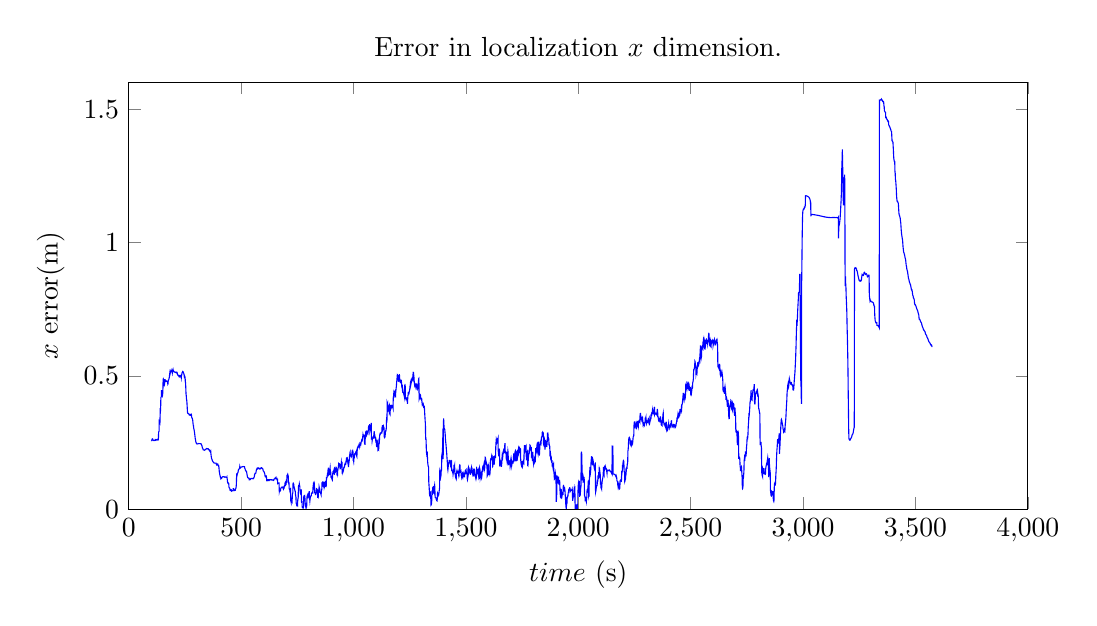
\begin{tikzpicture}

\begin{axis}[
title={Error in localization $x$ dimension.},
xlabel={$time$ (s)},
ylabel={$x$ error(m)},
xmin=0, xmax=4000,
ymin=0, ymax=1.6,
axis on top,
width=13cm,
height=7cm
]
\addplot [blue]
coordinates {
(100,0.257182079273758)
(101,0.256735420563738)
(102,0.256891980675641)
(103,0.256965842931189)
(104,0.262946582515819)
(105,0.263222172184873)
(106,0.263495503062185)
(107,0.259360605870688)
(108,0.259312773593893)
(109,0.259084900679902)
(110,0.258791082701098)
(111,0.257847812951566)
(112,0.257000868906019)
(113,0.257128593123862)
(114,0.257076876139985)
(115,0.257556624971283)
(116,0.258351531390327)
(117,0.25845276993058)
(118,0.260674387336823)
(119,0.259789122852471)
(120,0.25909169459993)
(121,0.258417000679683)
(122,0.259664861881095)
(123,0.259128630823634)
(124,0.259818252622826)
(125,0.26071880839572)
(126,0.261502363390435)
(127,0.261705856216593)
(128,0.261885691400126)
(129,0.259570053355544)
(130,0.258936439575621)
(131,0.259455299511213)
(132,0.260091201282002)
(133,0.2882993199319)
(134,0.290045222183811)
(135,0.291853481987137)
(136,0.332124708233765)
(137,0.33149763250479)
(138,0.328988860729536)
(139,0.326116252955655)
(140,0.367955142009396)
(141,0.365570532815856)
(142,0.3731753620158)
(143,0.418829055889278)
(144,0.419993046650572)
(145,0.421951246820612)
(146,0.44604289742549)
(147,0.439939772711337)
(148,0.431844726877102)
(149,0.427920237845144)
(150,0.425693177979303)
(151,0.432712494599663)
(152,0.438244205287286)
(153,0.485422326800568)
(154,0.488449651038288)
(155,0.486534053464957)
(156,0.47982885219792)
(157,0.465065102969197)
(158,0.463942448794136)
(159,0.467252398748453)
(160,0.482258548700048)
(161,0.485351788078082)
(162,0.48545414499389)
(163,0.482558497728577)
(164,0.478212076982257)
(165,0.478492455247137)
(166,0.480137156864327)
(167,0.48089780149699)
(168,0.480268500552255)
(169,0.478792898413062)
(170,0.478513970670941)
(171,0.478820052207523)
(172,0.47901166770857)
(173,0.478222929557619)
(174,0.468714844168443)
(175,0.470240324733756)
(176,0.483311142682501)
(177,0.483511985361489)
(178,0.484975801894698)
(179,0.488816742608635)
(180,0.49187789970772)
(181,0.496186230895613)
(182,0.504512930019551)
(183,0.511262332461044)
(184,0.50696855496147)
(185,0.510780565459715)
(186,0.515273819095719)
(187,0.518701487965101)
(188,0.517716351705937)
(189,0.520914662728896)
(190,0.518101309469002)
(191,0.516875407233449)
(192,0.51582851047123)
(193,0.515681960706349)
(194,0.511124661987533)
(195,0.518023434328427)
(196,0.522814892305151)
(197,0.524966457144986)
(198,0.520582169982935)
(199,0.518874904666205)
(200,0.517398106181032)
(201,0.517078148522321)
(202,0.514195564398927)
(203,0.514192373443186)
(204,0.514174028319191)
(205,0.514271105038067)
(206,0.513894392888159)
(207,0.513235486748284)
(208,0.513573180721848)
(209,0.512981948430386)
(210,0.512375345015176)
(211,0.511288360837811)
(212,0.510861099377568)
(213,0.513846944114412)
(214,0.513709882907484)
(215,0.513229135024102)
(216,0.509576475354696)
(217,0.50449043764081)
(218,0.504074482189742)
(219,0.502085855644496)
(220,0.500771375474822)
(221,0.500034811549684)
(222,0.502231398495387)
(223,0.501918354420803)
(224,0.501589793774539)
(225,0.496256927563469)
(226,0.497167922203096)
(227,0.497156266791335)
(228,0.49667272847588)
(229,0.499772450756123)
(230,0.499268336967517)
(231,0.498791837145174)
(232,0.500317730923353)
(233,0.499332261435188)
(234,0.493923280391825)
(235,0.504085446679958)
(236,0.504293454953923)
(237,0.510312033917289)
(238,0.51275173075926)
(239,0.513138774986377)
(240,0.516456807638455)
(241,0.515863055200658)
(242,0.514086680807075)
(243,0.51393749088891)
(244,0.510251999425174)
(245,0.508642284925086)
(246,0.504593546500138)
(247,0.498740812362605)
(248,0.492340468563589)
(249,0.492340996000868)
(250,0.495727530131909)
(251,0.49321274612838)
(252,0.474723117766731)
(253,0.47471015734792)
(254,0.453550053900914)
(255,0.431892856029436)
(256,0.425343547141554)
(257,0.412601114501605)
(258,0.409632602947367)
(259,0.400440810466923)
(260,0.386239180549588)
(261,0.369928187547202)
(262,0.360089237261416)
(263,0.359734188137496)
(264,0.359291291808822)
(265,0.358512124772201)
(266,0.35809219526888)
(267,0.356992335769933)
(268,0.357197178179422)
(269,0.354174071032281)
(270,0.354803328457873)
(271,0.354726175864125)
(272,0.354319380236194)
(273,0.351758981895121)
(274,0.351773385487262)
(275,0.352055026318059)
(276,0.351554429741805)
(277,0.356087815606904)
(278,0.356484916857232)
(279,0.354469943008377)
(280,0.345742712302354)
(281,0.342054480258617)
(282,0.340931895767489)
(283,0.340446052877782)
(284,0.336674626966255)
(285,0.332000294324344)
(286,0.322145610292039)
(287,0.315583865815446)
(288,0.313937280995534)
(289,0.305507497804515)
(290,0.30035976174916)
(291,0.297568054154723)
(292,0.29117711745903)
(293,0.28643561341642)
(294,0.278679939366798)
(295,0.272761578204924)
(296,0.264799859281497)
(297,0.260866196923816)
(298,0.255635247052329)
(299,0.250519695826455)
(300,0.249129375364056)
(301,0.247721837144807)
(302,0.244917882042729)
(303,0.244576452610509)
(304,0.244509484641122)
(305,0.244349961450218)
(306,0.244714057283619)
(307,0.24466114650134)
(308,0.245802031322228)
(309,0.245281204943963)
(310,0.245913053275173)
(311,0.245784152852319)
(312,0.245799611841649)
(313,0.245763103078974)
(314,0.245712308384897)
(315,0.245769401724972)
(316,0.245720020335478)
(317,0.245602635938983)
(318,0.24561976932218)
(319,0.245375925069988)
(320,0.245279965521059)
(321,0.245519121925484)
(322,0.245092801141051)
(323,0.242386466504643)
(324,0.241531826261234)
(325,0.238842459328023)
(326,0.237117668332579)
(327,0.233085075934389)
(328,0.229215405195821)
(329,0.228677278328525)
(330,0.227332599826632)
(331,0.223188458207272)
(332,0.222321999965579)
(333,0.222107990841118)
(334,0.221859076712366)
(335,0.221461522271196)
(336,0.22114342175743)
(337,0.221025876242169)
(338,0.220972340535299)
(339,0.221067546209294)
(340,0.223421547302572)
(341,0.223571260774405)
(342,0.224721450079923)
(343,0.224752930150255)
(344,0.22495676689097)
(345,0.225247236914588)
(346,0.225662098378234)
(347,0.227212169551507)
(348,0.226811112621059)
(349,0.226572909828025)
(350,0.226300846423321)
(351,0.226798845963377)
(352,0.226244211680713)
(353,0.226522235016532)
(354,0.226155949617924)
(355,0.22250919767371)
(356,0.222561264681325)
(357,0.222972786691395)
(358,0.222389515331942)
(359,0.222202320172608)
(360,0.221238796654947)
(361,0.216486534515495)
(362,0.215432914779496)
(363,0.214558671420501)
(364,0.213304714872298)
(365,0.215562317641765)
(366,0.20593928552998)
(367,0.198669262429661)
(368,0.193106888205735)
(369,0.189177670195488)
(370,0.187628574163072)
(371,0.186163610358388)
(372,0.181991178387899)
(373,0.181046365574001)
(374,0.17920629430474)
(375,0.1779013970178)
(376,0.17644607139383)
(377,0.17563477021213)
(378,0.174983753937468)
(379,0.173250951098767)
(380,0.173137148785049)
(381,0.172996176175681)
(382,0.172763916967381)
(383,0.172530057633238)
(384,0.172519716331041)
(385,0.172710540348168)
(386,0.172716706500218)
(387,0.172774603891809)
(388,0.172745127217133)
(389,0.172690661268673)
(390,0.167785987584718)
(391,0.165606343767807)
(392,0.165564702127379)
(393,0.165437776077722)
(394,0.169790652936417)
(395,0.169870649583416)
(396,0.169615550795915)
(397,0.165748734001008)
(398,0.165428351415392)
(399,0.163554962931759)
(400,0.161061077933378)
(401,0.161333371042074)
(402,0.150313033930009)
(403,0.141206198984659)
(404,0.135897721545775)
(405,0.130657903229931)
(406,0.126635452837976)
(407,0.124188827282921)
(408,0.118649646626332)
(409,0.118056640821835)
(410,0.114042621415804)
(411,0.115157270096508)
(412,0.114308037047983)
(413,0.114317333458383)
(414,0.117880641228115)
(415,0.119256991604095)
(416,0.120823623578423)
(417,0.121097368726232)
(418,0.121619276710206)
(419,0.121639857861584)
(420,0.121894435815643)
(421,0.121609380069696)
(422,0.121539222999194)
(423,0.121403056159659)
(424,0.121541134060846)
(425,0.121337691282699)
(426,0.120167898540996)
(427,0.119782941968088)
(428,0.119696654772036)
(429,0.121030300144555)
(430,0.121099671357953)
(431,0.120218299519938)
(432,0.120271392230419)
(433,0.11982957933933)
(434,0.119081488920656)
(435,0.118887348522478)
(436,0.118229187093153)
(437,0.12039256384048)
(438,0.113589188538716)
(439,0.109885541065884)
(440,0.0982843776242373)
(441,0.0980958793873028)
(442,0.0973339723152762)
(443,0.0983419420198057)
(444,0.0971089561295759)
(445,0.0961424553960497)
(446,0.0826590263845741)
(447,0.0803232257968602)
(448,0.0797975025311644)
(449,0.0791365969418401)
(450,0.0774673332867484)
(451,0.0705605352107219)
(452,0.0703065896517701)
(453,0.0705376880955337)
(454,0.0731318059044397)
(455,0.073195656246996)
(456,0.0729940465624526)
(457,0.0671105700941066)
(458,0.0674406547961501)
(459,0.0675221068521283)
(460,0.0687535886981179)
(461,0.0695873454554383)
(462,0.0694713176703301)
(463,0.0693329336175577)
(464,0.069235685018703)
(465,0.0764474916793167)
(466,0.0764724150497926)
(467,0.0764717528197907)
(468,0.0718576048466146)
(469,0.0717947231294072)
(470,0.0717303825064359)
(471,0.0700468596939401)
(472,0.0701134288322143)
(473,0.0703591004998048)
(474,0.070522936770109)
(475,0.075339490151983)
(476,0.0764736764433698)
(477,0.0782716461764621)
(478,0.0834563137586932)
(479,0.0941880205203613)
(480,0.125061908565076)
(481,0.122748591420945)
(482,0.127652688893642)
(483,0.130450581809223)
(484,0.134355516997186)
(485,0.135881848879694)
(486,0.137357785658209)
(487,0.141417883259775)
(488,0.147804859278495)
(489,0.148891653440351)
(490,0.150228471986362)
(491,0.150415122562956)
(492,0.151151013211556)
(493,0.152192463735552)
(494,0.158809385773527)
(495,0.154345337271975)
(496,0.153937806911748)
(497,0.153882801615896)
(498,0.157646982250133)
(499,0.157523690012724)
(500,0.15764309275547)
(501,0.157566543729251)
(502,0.157866193309804)
(503,0.158507157821586)
(504,0.158788549322484)
(505,0.158728971446645)
(506,0.158886506762222)
(507,0.159165172834363)
(508,0.159105099283396)
(509,0.160078660812326)
(510,0.159672766652991)
(511,0.159688986035948)
(512,0.159503754415765)
(513,0.159412173305169)
(514,0.159456214314529)
(515,0.159336946257134)
(516,0.154234791418278)
(517,0.152754729095906)
(518,0.149669542419248)
(519,0.147477142381682)
(520,0.14421132865302)
(521,0.143785693037186)
(522,0.143439151678097)
(523,0.141641646981205)
(524,0.141212386882705)
(525,0.136491338737115)
(526,0.132463674936627)
(527,0.126917364131953)
(528,0.122494388253733)
(529,0.118833895776105)
(530,0.118126006316272)
(531,0.11785443843443)
(532,0.116542502431355)
(533,0.116524027768655)
(534,0.116350803132155)
(535,0.116158412879304)
(536,0.109885939179058)
(537,0.109948171387609)
(538,0.110218239379909)
(539,0.11334068883146)
(540,0.113042085506732)
(541,0.112896006884021)
(542,0.112098157604532)
(543,0.114710626663222)
(544,0.114832883344038)
(545,0.115012887654787)
(546,0.115249032904646)
(547,0.115396299835321)
(548,0.115357864229948)
(549,0.114789582994243)
(550,0.114859932214414)
(551,0.114796678943211)
(552,0.114747667399003)
(553,0.113965620576708)
(554,0.114885014316905)
(555,0.115334851164951)
(556,0.115959411830139)
(557,0.11896513001121)
(558,0.119916387039353)
(559,0.121252732436997)
(560,0.130593041249353)
(561,0.131865613017426)
(562,0.133756748036415)
(563,0.133120179366741)
(564,0.133535144256244)
(565,0.134779945980853)
(566,0.138140623384441)
(567,0.1413491830358)
(568,0.147866982290432)
(569,0.149107398479886)
(570,0.150290614358284)
(571,0.152110911954665)
(572,0.150464331862101)
(573,0.150670462022583)
(574,0.15067307058664)
(575,0.151146041135986)
(576,0.154836216156639)
(577,0.15457176428603)
(578,0.154728730002601)
(579,0.152758447988116)
(580,0.152556388577501)
(581,0.152461057434879)
(582,0.152027917112435)
(583,0.150258710573288)
(584,0.150399900181658)
(585,0.15062859267815)
(586,0.153126003711474)
(587,0.15306232277906)
(588,0.153558493446515)
(589,0.153561472063979)
(590,0.155826752271198)
(591,0.155865938879218)
(592,0.155812320369411)
(593,0.15324814707925)
(594,0.152246294223192)
(595,0.151946949246028)
(596,0.15163368938211)
(597,0.149487300168546)
(598,0.145170520586448)
(599,0.142841888252545)
(600,0.142328970601677)
(601,0.141672558033298)
(602,0.139468802500899)
(603,0.138366718655113)
(604,0.135652932383192)
(605,0.133394720866999)
(606,0.128897608663176)
(607,0.122024386680366)
(608,0.121524046347623)
(609,0.124550301223395)
(610,0.124303291382695)
(611,0.124422701957452)
(612,0.124514980654231)
(613,0.118204497911402)
(614,0.10750696050934)
(615,0.106444987097663)
(616,0.108003459537612)
(617,0.108115157834924)
(618,0.108111041308584)
(619,0.110323135964433)
(620,0.110375632947882)
(621,0.110371856837307)
(622,0.106931974264896)
(623,0.106953112966889)
(624,0.106735563196447)
(625,0.10675923909115)
(626,0.110135450704676)
(627,0.110341429079453)
(628,0.110454710946951)
(629,0.110489016376216)
(630,0.110469212327053)
(631,0.110476214268623)
(632,0.110452948889195)
(633,0.108629278425934)
(634,0.108665376505457)
(635,0.110141251503952)
(636,0.110360873120207)
(637,0.110566111297512)
(638,0.109596133512357)
(639,0.109066410130657)
(640,0.108911680735476)
(641,0.109031502356605)
(642,0.109117970196083)
(643,0.10748668346068)
(644,0.107527559942511)
(645,0.107662834708219)
(646,0.111890496828688)
(647,0.112538939617784)
(648,0.113228593771869)
(649,0.113919759932174)
(650,0.115181939357651)
(651,0.116208490108427)
(652,0.116677623856049)
(653,0.117639814998705)
(654,0.118265071566825)
(655,0.119210590426003)
(656,0.11420946626934)
(657,0.114911234945273)
(658,0.115016978636978)
(659,0.115224976651142)
(660,0.11133283281931)
(661,0.112389296869929)
(662,0.112408636178746)
(663,0.0958559434171335)
(664,0.0963973866205508)
(665,0.0969569152697112)
(666,0.0977565481994849)
(667,0.0980505935361333)
(668,0.0974628282497734)
(669,0.0976853236827186)
(670,0.0660718553594006)
(671,0.0697821435298813)
(672,0.0703144874999402)
(673,0.0708869196758437)
(674,0.0679468005530079)
(675,0.0685628675022874)
(676,0.0756425849485831)
(677,0.078308487407861)
(678,0.0800197031571863)
(679,0.0816456006774176)
(680,0.0824484824953293)
(681,0.0822595021185402)
(682,0.0824113890530125)
(683,0.0817112659861601)
(684,0.0814965966024426)
(685,0.0824285494789683)
(686,0.0799336814325637)
(687,0.0818816941477349)
(688,0.0786573146175638)
(689,0.0752248437717742)
(690,0.0770352978404252)
(691,0.0781028111772808)
(692,0.0831423808093601)
(693,0.0843353162177061)
(694,0.0871403286771124)
(695,0.0943937366375396)
(696,0.09965157693459)
(697,0.100915110740612)
(698,0.0953480683587244)
(699,0.0910903701384322)
(700,0.0920308707503796)
(701,0.102357037966669)
(702,0.100018144877647)
(703,0.101555310610029)
(704,0.125925790646344)
(705,0.126731515331972)
(706,0.128591558111257)
(707,0.12486985232852)
(708,0.128567013502374)
(709,0.125062170522623)
(710,0.12354681905462)
(711,0.0984967377313617)
(712,0.0961895121060978)
(713,0.0968566424788788)
(714,0.0766939755242073)
(715,0.0743845841412201)
(716,0.073230859673822)
(717,0.0742128463822533)
(718,0.0627932387197507)
(719,0.0609735053059866)
(720,0.0652489003141552)
(721,0.0315827685164143)
(722,0.0289461245682401)
(723,0.0245720859367795)
(724,0.0322813343571386)
(725,0.0343452072051971)
(726,0.0334682890383831)
(727,0.0308103658691863)
(728,0.0554286256529615)
(729,0.0585588743237242)
(730,0.0609166111245751)
(731,0.0953395056863275)
(732,0.0974955417722057)
(733,0.0963449655123809)
(734,0.0936896290966409)
(735,0.0865914308883515)
(736,0.0798094607460422)
(737,0.0795721981174506)
(738,0.0765322231599406)
(739,0.0712140794278593)
(740,0.0679795519728521)
(741,0.0673248581430745)
(742,0.0530488768126105)
(743,0.0501147043807881)
(744,0.0449996741537655)
(745,0.0223742985274762)
(746,0.0215967969959632)
(747,0.0171330017234719)
(748,0.0188062917647982)
(749,0.0142415660865503)
(750,0.0151483404828161)
(751,0.0138801490409866)
(752,0.0339473527157801)
(753,0.0385372402855584)
(754,0.0425995824075782)
(755,0.0850359072529696)
(756,0.0881663587517636)
(757,0.0881394573876944)
(758,0.0895123677648706)
(759,0.0948017857475825)
(760,0.0896418114645243)
(761,0.0861256497835119)
(762,0.0707568691451259)
(763,0.0664203818679394)
(764,0.0589148934089079)
(765,0.0570592589950483)
(766,0.0722742711458642)
(767,0.072432597644684)
(768,0.07085923628228)
(769,0.0237380747838514)
(770,0.0288507534216329)
(771,0.0285068031036046)
(772,0.0078222609239833)
(773,0.00618026188476906)
(774,0.00608674854910696)
(775,0.00475048318511595)
(776,0.00387066708441042)
(777,0.00679302943699023)
(778,0.00999537549883067)
(779,0.0481001212995977)
(780,0.0497869098217776)
(781,0.0503026930346349)
(782,0.0479622075665045)
(783,0.0492496811182472)
(784,0.0420651592297729)
(785,0.0259276546178202)
(786,0.013390554375881)
(787,0.012711485860478)
(788,0.00680919334768637)
(789,0.0034256011973115)
(790,0.0168402683713271)
(791,0.00579151702423975)
(792,0.0143803884278157)
(793,0.0453187361998171)
(794,0.0484948105298342)
(795,0.0461278337145976)
(796,0.0513404874692895)
(797,0.0497873651477878)
(798,0.0591504378869123)
(799,0.0595159425389276)
(800,0.0502238770467796)
(801,0.0526602981414337)
(802,0.0533771537959207)
(803,0.0671718546142483)
(804,0.0404604388382697)
(805,0.0397990994644055)
(806,0.0309342377228075)
(807,0.0388315817695823)
(808,0.0439315919526044)
(809,0.0469318839141799)
(810,0.0491085287597874)
(811,0.0495237919998841)
(812,0.0498265071507982)
(813,0.0574000120058127)
(814,0.0593354286860808)
(815,0.0608486195353675)
(816,0.061581670561158)
(817,0.063668804742171)
(818,0.0633684418528442)
(819,0.0581713512502637)
(820,0.0815015368282332)
(821,0.087509784159661)
(822,0.0959564558979906)
(823,0.093694067219757)
(824,0.0900769413055613)
(825,0.0907015042545209)
(826,0.0936131922021617)
(827,0.0643009887499075)
(828,0.0608128738181706)
(829,0.0603911737853013)
(830,0.0609493547946602)
(831,0.0553682374808377)
(832,0.0549322914001968)
(833,0.0575380083947477)
(834,0.0647577698946153)
(835,0.075580153898291)
(836,0.0767698881816004)
(837,0.0758488236223478)
(838,0.0698383492219543)
(839,0.0726125120722259)
(840,0.0714418683673825)
(841,0.0447359051908975)
(842,0.0447093857408367)
(843,0.0437924924159123)
(844,0.0672689691932917)
(845,0.0660678881467449)
(846,0.0704062307206752)
(847,0.0833805801345679)
(848,0.0792936785160157)
(849,0.0771093328723436)
(850,0.074696950781552)
(851,0.0630137160263087)
(852,0.0628516612867651)
(853,0.061370228655881)
(854,0.0589171105231592)
(855,0.0568940576680554)
(856,0.0538524643851943)
(857,0.0654860882322335)
(858,0.0697059578194352)
(859,0.0744981681758419)
(860,0.0966596120651309)
(861,0.0959527669267297)
(862,0.0982138664996999)
(863,0.104173479413021)
(864,0.0870971815096424)
(865,0.0862333275766907)
(866,0.0850574327565177)
(867,0.0945864918305208)
(868,0.0941746227706761)
(869,0.102517406317224)
(870,0.080456472857616)
(871,0.0830066806842868)
(872,0.0943612272147032)
(873,0.0935041352652184)
(874,0.0962361961008784)
(875,0.100924035146547)
(876,0.106152962332001)
(877,0.0850932027179274)
(878,0.0848044894652333)
(879,0.0892778085236281)
(880,0.116827139754057)
(881,0.116143822510984)
(882,0.117932947585152)
(883,0.121980794707836)
(884,0.131865805228754)
(885,0.135177114443831)
(886,0.136396966831759)
(887,0.148691442973871)
(888,0.152126091108054)
(889,0.150633211278368)
(890,0.129515129755166)
(891,0.131251238305185)
(892,0.133453647395945)
(893,0.127625501766127)
(894,0.143136782110376)
(895,0.148733332074001)
(896,0.154515803306089)
(897,0.139975020904337)
(898,0.138323392154192)
(899,0.138234644762343)
(900,0.121917422900903)
(901,0.122433869119935)
(902,0.119311854686664)
(903,0.115945905690129)
(904,0.115216940622076)
(905,0.110584755430098)
(906,0.109118710316155)
(907,0.126944743959102)
(908,0.134606719565054)
(909,0.140899829141279)
(910,0.141986027897996)
(911,0.143284717364336)
(912,0.143341291898849)
(913,0.146403567946478)
(914,0.132510694140934)
(915,0.131329357789424)
(916,0.132495462027029)
(917,0.142813554448733)
(918,0.138080399620361)
(919,0.138047326370899)
(920,0.140329562892655)
(921,0.152145260153948)
(922,0.15717607923834)
(923,0.157087312114389)
(924,0.152258116436161)
(925,0.150615979770297)
(926,0.149652579116425)
(927,0.12549117183958)
(928,0.132769571771786)
(929,0.129854035699574)
(930,0.147937202186843)
(931,0.150065480038061)
(932,0.154576111905092)
(933,0.158903483835397)
(934,0.16993757511985)
(935,0.168631300141873)
(936,0.169978821615719)
(937,0.170350639419687)
(938,0.168956378286766)
(939,0.167584769479083)
(940,0.15653957509145)
(941,0.158473579534683)
(942,0.157019318674613)
(943,0.1550330721846)
(944,0.161225738084071)
(945,0.166674221169238)
(946,0.174984291232915)
(947,0.167177504954766)
(948,0.166706841033156)
(949,0.168764160117356)
(950,0.140473016942027)
(951,0.142436431013001)
(952,0.136516079702306)
(953,0.139284556474007)
(954,0.140856155463755)
(955,0.143889840022998)
(956,0.149222280010015)
(957,0.156248861090044)
(958,0.15727099135346)
(959,0.156696090909226)
(960,0.158677520162902)
(961,0.166174100224298)
(962,0.168874759060632)
(963,0.166520825752881)
(964,0.167111297125489)
(965,0.168808095600124)
(966,0.168958457941035)
(967,0.18056958450841)
(968,0.184272453021251)
(969,0.190911044079071)
(970,0.191935643882407)
(971,0.192831543616415)
(972,0.193211576925478)
(973,0.182714301067481)
(974,0.184425696950361)
(975,0.183046875250566)
(976,0.167125875892814)
(977,0.167413146762349)
(978,0.157764180315527)
(979,0.170394900206247)
(980,0.175186269322338)
(981,0.18211282885124)
(982,0.197531896682203)
(983,0.197883487510727)
(984,0.209796265518788)
(985,0.213127263755989)
(986,0.200997671834447)
(987,0.200400370676483)
(988,0.200034066931716)
(989,0.20038830128903)
(990,0.195335241491918)
(991,0.196732457579861)
(992,0.202843129064664)
(993,0.209536088542528)
(994,0.215105639117027)
(995,0.213526996990422)
(996,0.214636537087611)
(997,0.217752839422181)
(998,0.214099195995963)
(999,0.182670172217606)
(1000,0.18256458692785)
(1001,0.178038565389694)
(1002,0.189179943395525)
(1003,0.190649364887094)
(1004,0.200211193781132)
(1005,0.207062670840264)
(1006,0.207256075827108)
(1007,0.207942165726647)
(1008,0.207462173997595)
(1009,0.211043548205685)
(1010,0.209798490476949)
(1011,0.213911406470198)
(1012,0.215978215717911)
(1013,0.200212219691235)
(1014,0.199607382012445)
(1015,0.197232321999042)
(1016,0.209877158326429)
(1017,0.228125149904227)
(1018,0.231387031379441)
(1019,0.230942967912253)
(1020,0.232039050523206)
(1021,0.236856546463301)
(1022,0.237261020783314)
(1023,0.237109892651953)
(1024,0.240325142021462)
(1025,0.238428457880162)
(1026,0.232417757804211)
(1027,0.235530832153477)
(1028,0.242623820066071)
(1029,0.239662448800315)
(1030,0.24542385729257)
(1031,0.247787457085264)
(1032,0.24754083165285)
(1033,0.245055603569371)
(1034,0.250791825444889)
(1035,0.253255424791537)
(1036,0.256558235249742)
(1037,0.260787292695943)
(1038,0.260274320769317)
(1039,0.258295127473406)
(1040,0.262165053771841)
(1041,0.270423823733899)
(1042,0.27753532105219)
(1043,0.271504840118949)
(1044,0.271373616410386)
(1045,0.271268991642614)
(1046,0.273257020438251)
(1047,0.27427021445913)
(1048,0.279625381377127)
(1049,0.250877565090003)
(1050,0.246761349766687)
(1051,0.241247135112344)
(1052,0.261767813895497)
(1053,0.269631426041077)
(1054,0.285092170877572)
(1055,0.290657122249844)
(1056,0.291593296256268)
(1057,0.292559046369354)
(1058,0.291172119081611)
(1059,0.282157238734703)
(1060,0.286592854750733)
(1061,0.289057047488105)
(1062,0.290361721717218)
(1063,0.285420404960717)
(1064,0.283542006391196)
(1065,0.290139039123972)
(1066,0.294200363101706)
(1067,0.307864538442613)
(1068,0.310916408908922)
(1069,0.3099226809136)
(1070,0.306108147941213)
(1071,0.312430063580262)
(1072,0.318504167605519)
(1073,0.292738380476055)
(1074,0.29646444902495)
(1075,0.300155244102403)
(1076,0.301878966309332)
(1077,0.303176182505213)
(1078,0.309778167458709)
(1079,0.323144905317641)
(1080,0.261166563952658)
(1081,0.266504935189174)
(1082,0.273318988190874)
(1083,0.256376544071414)
(1084,0.261504258356585)
(1085,0.266031448500654)
(1086,0.266010959846369)
(1087,0.266823469725723)
(1088,0.266122772829734)
(1089,0.266680120409198)
(1090,0.272892875202907)
(1091,0.280960859389222)
(1092,0.292045869905169)
(1093,0.280595729683462)
(1094,0.279303143485657)
(1095,0.278226867011102)
(1096,0.265751841977237)
(1097,0.265325737481195)
(1098,0.26641874789656)
(1099,0.257777999701508)
(1100,0.259742579040704)
(1101,0.25003761074805)
(1102,0.247236731094968)
(1103,0.232575840466114)
(1104,0.244695324580069)
(1105,0.251344542477865)
(1106,0.248658287351675)
(1107,0.250741611247819)
(1108,0.25339726685528)
(1109,0.223054262072532)
(1110,0.224582607379287)
(1111,0.224116100510424)
(1112,0.222785965608579)
(1113,0.243810457689088)
(1114,0.2444080534935)
(1115,0.24859439664068)
(1116,0.269424188945388)
(1117,0.278444369830779)
(1118,0.281930568085359)
(1119,0.280786126968099)
(1120,0.281486253939428)
(1121,0.2854277253015)
(1122,0.286423820186319)
(1123,0.286579851339197)
(1124,0.288590888529844)
(1125,0.289052229420288)
(1126,0.283268832878476)
(1127,0.306304810906035)
(1128,0.307536847926552)
(1129,0.315257426930655)
(1130,0.297299040536871)
(1131,0.299582529969241)
(1132,0.310619440559439)
(1133,0.312222976839245)
(1134,0.307301370226109)
(1135,0.306095132257313)
(1136,0.303917464821863)
(1137,0.271548093389809)
(1138,0.267498407461286)
(1139,0.267999158428144)
(1140,0.271064029045851)
(1141,0.27819157086653)
(1142,0.287522554416269)
(1143,0.293015338505211)
(1144,0.292917701760162)
(1145,0.29740699299493)
(1146,0.30312478314768)
(1147,0.334285107359528)
(1148,0.343350080632754)
(1149,0.340209610924816)
(1150,0.393030056294112)
(1151,0.388564879436717)
(1152,0.392260134206874)
(1153,0.363870721307229)
(1154,0.372810211699319)
(1155,0.378197544697946)
(1156,0.37780040808804)
(1157,0.385189786751322)
(1158,0.388002997407261)
(1159,0.390262394257278)
(1160,0.363120095003369)
(1161,0.36612562053247)
(1162,0.365865597934341)
(1163,0.362139145334416)
(1164,0.381750451567306)
(1165,0.384294036546665)
(1166,0.391093756050324)
(1167,0.374142860637436)
(1168,0.38093046261995)
(1169,0.380355954151888)
(1170,0.380477602780687)
(1171,0.384554134117465)
(1172,0.388912127143395)
(1173,0.388556519773587)
(1174,0.383432696740569)
(1175,0.384267886271715)
(1176,0.380166706243599)
(1177,0.41788289004668)
(1178,0.42058048103674)
(1179,0.431345941067661)
(1180,0.439925914874052)
(1181,0.437556739444415)
(1182,0.435856286148803)
(1183,0.438259684787718)
(1184,0.440054765965326)
(1185,0.423068736964783)
(1186,0.424407310625752)
(1187,0.423325918843883)
(1188,0.440666915116301)
(1189,0.446801830920817)
(1190,0.455249524278339)
(1191,0.462306671274739)
(1192,0.475986372902789)
(1193,0.482660280838124)
(1194,0.492703814978818)
(1195,0.487942211588831)
(1196,0.487511401615334)
(1197,0.501405834223117)
(1198,0.499833574908431)
(1199,0.485580769970958)
(1200,0.48033357437755)
(1201,0.479632051115614)
(1202,0.480555048754047)
(1203,0.480812186047404)
(1204,0.506501300425338)
(1205,0.498978679184556)
(1206,0.483258138998738)
(1207,0.479344645943879)
(1208,0.480423663942072)
(1209,0.476247478226378)
(1210,0.475077710441824)
(1211,0.484041491519229)
(1212,0.484030924826745)
(1213,0.48164325071156)
(1214,0.470283585965512)
(1215,0.459042605266935)
(1216,0.460233395369076)
(1217,0.461544492124527)
(1218,0.447585778890688)
(1219,0.450572714969597)
(1220,0.445163758372292)
(1221,0.437486971203004)
(1222,0.436914365390468)
(1223,0.433769608987421)
(1224,0.430121593256509)
(1225,0.426507152387884)
(1226,0.423187391349136)
(1227,0.419005907740242)
(1228,0.464492193252597)
(1229,0.466007402372338)
(1230,0.464208671364928)
(1231,0.417782354532114)
(1232,0.416322130149133)
(1233,0.416926436570977)
(1234,0.414159494985077)
(1235,0.417300086494953)
(1236,0.416444872814439)
(1237,0.413361814267027)
(1238,0.41188181667681)
(1239,0.408108889459493)
(1240,0.394941557410806)
(1241,0.410476338441371)
(1242,0.424267309477426)
(1243,0.427731773168157)
(1244,0.439167680301336)
(1245,0.431749061940383)
(1246,0.431491296738061)
(1247,0.434251751184494)
(1248,0.440314673014829)
(1249,0.443687476809347)
(1250,0.447530021358634)
(1251,0.455919150106944)
(1252,0.454943662994329)
(1253,0.469891482950717)
(1254,0.476498196327396)
(1255,0.479510656590699)
(1256,0.470400138566609)
(1257,0.47469474168318)
(1258,0.477740098381695)
(1259,0.480536275551005)
(1260,0.485296945341187)
(1261,0.49091175017072)
(1262,0.494005853734047)
(1263,0.494183437644902)
(1264,0.490446670860478)
(1265,0.505801815103425)
(1266,0.512533497738633)
(1267,0.511811595874692)
(1268,0.502756094906941)
(1269,0.495263531835826)
(1270,0.482430270257709)
(1271,0.471403243661695)
(1272,0.465273522255807)
(1273,0.468620828632985)
(1274,0.464718737206666)
(1275,0.465232953277016)
(1276,0.462159552523167)
(1277,0.458505045213872)
(1278,0.467268026806603)
(1279,0.469346821440712)
(1280,0.46808850484732)
(1281,0.465374632010808)
(1282,0.459876985853424)
(1283,0.452880203128883)
(1284,0.449568220401916)
(1285,0.451620950305424)
(1286,0.464292477540391)
(1287,0.468684099013517)
(1288,0.470172521749687)
(1289,0.477907876429184)
(1290,0.489431292476061)
(1291,0.490665146570226)
(1292,0.41232145598647)
(1293,0.414948083908836)
(1294,0.4157878833713)
(1295,0.422353310411971)
(1296,0.427068011324148)
(1297,0.425307162309033)
(1298,0.426653756978997)
(1299,0.414137030023251)
(1300,0.413547061078888)
(1301,0.41166032267876)
(1302,0.415962168087204)
(1303,0.415729006067886)
(1304,0.410067894041568)
(1305,0.398971429132685)
(1306,0.391218963502906)
(1307,0.392762890097063)
(1308,0.393239585498291)
(1309,0.395696846239209)
(1310,0.396376421028263)
(1311,0.389006332919996)
(1312,0.382016892336944)
(1313,0.382510492118487)
(1314,0.381544812487448)
(1315,0.38821570921343)
(1316,0.37337673831686)
(1317,0.356693849534005)
(1318,0.344017762132962)
(1319,0.329270453103498)
(1320,0.321703286984713)
(1321,0.260602041626252)
(1322,0.265412333874146)
(1323,0.258765209479639)
(1324,0.226523641350051)
(1325,0.21152270759122)
(1326,0.20495253766248)
(1327,0.207638212498952)
(1328,0.215559934302491)
(1329,0.196286517892012)
(1330,0.177642491718739)
(1331,0.168585199224323)
(1332,0.16338934737341)
(1333,0.158825297748306)
(1334,0.158374078437531)
(1335,0.102280211583207)
(1336,0.0899756975277528)
(1337,0.0771877185814689)
(1338,0.0609915651895774)
(1339,0.0476518098781678)
(1340,0.0550341908253644)
(1341,0.0671183812823135)
(1342,0.0588943809558695)
(1343,0.0413244512912581)
(1344,0.039163189906243)
(1345,0.0152553134702127)
(1346,0.0166845224863406)
(1347,0.0208158116598658)
(1348,0.0303093505193712)
(1349,0.0692701847396191)
(1350,0.0592483596397972)
(1351,0.0581781859821446)
(1352,0.0739670029058828)
(1353,0.0821364811404508)
(1354,0.0829852841055527)
(1355,0.0715002295533345)
(1356,0.0607852696102853)
(1357,0.0599280109836444)
(1358,0.0666302371855574)
(1359,0.0664703831449436)
(1360,0.083963572023201)
(1361,0.0892542593368049)
(1362,0.0810135498117219)
(1363,0.0469770800395954)
(1364,0.0437587057953643)
(1365,0.0439225252758901)
(1366,0.042748402118121)
(1367,0.0423738506200113)
(1368,0.0374618541957479)
(1369,0.0374925689994097)
(1370,0.0330281207243539)
(1371,0.0336981193872026)
(1372,0.0324994820604996)
(1373,0.0393936870541056)
(1374,0.0598440898974357)
(1375,0.0576923388456101)
(1376,0.0566181413284932)
(1377,0.058428940778235)
(1378,0.0578785861596836)
(1379,0.0539511539307136)
(1380,0.0582131440686591)
(1381,0.0666879578725537)
(1382,0.0726725554530536)
(1383,0.0788580965410035)
(1384,0.144105654695632)
(1385,0.141070968285692)
(1386,0.136848823340468)
(1387,0.129083498355353)
(1388,0.12034379207439)
(1389,0.124589386796865)
(1390,0.138829710971346)
(1391,0.153057446375721)
(1392,0.151656215663058)
(1393,0.20466083311209)
(1394,0.204550631325103)
(1395,0.211053150117565)
(1396,0.22524808966867)
(1397,0.247910034169044)
(1398,0.301762543888433)
(1399,0.187825228906956)
(1400,0.314949665980479)
(1401,0.340024849204281)
(1402,0.325412102140907)
(1403,0.302353630169386)
(1404,0.30118317835225)
(1405,0.301229159445336)
(1406,0.298914618186646)
(1407,0.289990874741406)
(1408,0.280566407545681)
(1409,0.265128193830388)
(1410,0.253480116973483)
(1411,0.247031550244233)
(1412,0.237157443702403)
(1413,0.226192530168719)
(1414,0.215987331212609)
(1415,0.206791894608442)
(1416,0.1923714126257)
(1417,0.182872070928612)
(1418,0.166051392222831)
(1419,0.153370963549449)
(1420,0.147261288361822)
(1421,0.154487687924711)
(1422,0.166764164291617)
(1423,0.168461538796502)
(1424,0.175008335618632)
(1425,0.176386016199609)
(1426,0.182517170743437)
(1427,0.182450662909545)
(1428,0.18230265610591)
(1429,0.177563989390791)
(1430,0.175726916550202)
(1431,0.168183234533115)
(1432,0.163340702758048)
(1433,0.167224245539554)
(1434,0.175822549966514)
(1435,0.182160055083503)
(1436,0.181472984882369)
(1437,0.142300813421816)
(1438,0.148849248973906)
(1439,0.145692878910823)
(1440,0.141220008669012)
(1441,0.138768627363718)
(1442,0.139950684219463)
(1443,0.131090284791619)
(1444,0.136927483124384)
(1445,0.140111597644833)
(1446,0.147477771877609)
(1447,0.160085330183797)
(1448,0.158352585744368)
(1449,0.1594465274903)
(1450,0.163668648255353)
(1451,0.134183492812131)
(1452,0.133570807198821)
(1453,0.127680475827001)
(1454,0.120429849414328)
(1455,0.117993222893323)
(1456,0.114359190269322)
(1457,0.112475385074846)
(1458,0.13315258998723)
(1459,0.138607249794251)
(1460,0.142618382508792)
(1461,0.134315536859879)
(1462,0.135084528601166)
(1463,0.141827411469995)
(1464,0.142024232775206)
(1465,0.141660396663035)
(1466,0.139831974986214)
(1467,0.141045093696804)
(1468,0.12747592617721)
(1469,0.12300930911544)
(1470,0.125475077054264)
(1471,0.157319974112218)
(1472,0.162181293779249)
(1473,0.165526212584851)
(1474,0.164796308026992)
(1475,0.135889371408454)
(1476,0.142457178271035)
(1477,0.142676153361915)
(1478,0.143813286372167)
(1479,0.128957482668841)
(1480,0.130085821290646)
(1481,0.127520545773668)
(1482,0.11551015376511)
(1483,0.117164295649838)
(1484,0.120471452231232)
(1485,0.13357565457133)
(1486,0.136900706339086)
(1487,0.138039392871153)
(1488,0.127003805849265)
(1489,0.132341647027296)
(1490,0.134538563907681)
(1491,0.133964374923286)
(1492,0.128322118818089)
(1493,0.12865043292157)
(1494,0.119531665598092)
(1495,0.131137126998129)
(1496,0.135693893261662)
(1497,0.143392663975115)
(1498,0.144733104666536)
(1499,0.140493806745072)
(1500,0.144069155263165)
(1501,0.146165196675392)
(1502,0.13530151438245)
(1503,0.13568432953685)
(1504,0.134560723425902)
(1505,0.134601954164676)
(1506,0.115415068099437)
(1507,0.110340985571882)
(1508,0.114147907181214)
(1509,0.144486150322305)
(1510,0.15304141771866)
(1511,0.155595971742494)
(1512,0.135588350889272)
(1513,0.140567854757668)
(1514,0.146432358937652)
(1515,0.148819072568511)
(1516,0.142818960884651)
(1517,0.141321839879225)
(1518,0.139760533627862)
(1519,0.131447220048634)
(1520,0.131179707768383)
(1521,0.135173739425243)
(1522,0.148443275072352)
(1523,0.151481180244488)
(1524,0.153597663392813)
(1525,0.156769040298681)
(1526,0.144372803588229)
(1527,0.146623670369241)
(1528,0.148188602878864)
(1529,0.133351725614619)
(1530,0.13391905723344)
(1531,0.12872648581074)
(1532,0.122515612189949)
(1533,0.139433602007577)
(1534,0.145261448545866)
(1535,0.15129637665813)
(1536,0.133969521052988)
(1537,0.130518441097503)
(1538,0.133788023745707)
(1539,0.138453838489406)
(1540,0.130763877614239)
(1541,0.129752607242788)
(1542,0.128957029156371)
(1543,0.120801521797052)
(1544,0.116268968447349)
(1545,0.112322906625933)
(1546,0.115866950128527)
(1547,0.146579968043336)
(1548,0.154375239714648)
(1549,0.152975849528318)
(1550,0.131332186182129)
(1551,0.133786596941744)
(1552,0.137204054388533)
(1553,0.141703500059696)
(1554,0.145807443748192)
(1555,0.144923063369395)
(1556,0.147249214244462)
(1557,0.123230166333679)
(1558,0.116247699806933)
(1559,0.118347660273224)
(1560,0.128195231257833)
(1561,0.154460938185968)
(1562,0.151251349374437)
(1563,0.146363944145535)
(1564,0.118507011466712)
(1565,0.123182950029107)
(1566,0.128115790264222)
(1567,0.131074686160065)
(1568,0.122062737811226)
(1569,0.121492074206063)
(1570,0.117550827187144)
(1571,0.122696583856173)
(1572,0.130269525744913)
(1573,0.14497827077922)
(1574,0.151122311575983)
(1575,0.145685981647771)
(1576,0.14458098209358)
(1577,0.147705754338303)
(1578,0.15865824099212)
(1579,0.162693914059637)
(1580,0.166919943861993)
(1581,0.156144808669074)
(1582,0.156743009179251)
(1583,0.150389660777372)
(1584,0.155596715394772)
(1585,0.180028806423983)
(1586,0.194565837703802)
(1587,0.194064355597703)
(1588,0.166821495817305)
(1589,0.174996368503801)
(1590,0.178840885733502)
(1591,0.175392794670735)
(1592,0.168496460447412)
(1593,0.165152600962511)
(1594,0.160932163678981)
(1595,0.124212017025365)
(1596,0.125984370052864)
(1597,0.138759823310077)
(1598,0.146167514458839)
(1599,0.157662172719141)
(1600,0.154444241414476)
(1601,0.15898074621151)
(1602,0.127900690865086)
(1603,0.135859947342943)
(1604,0.135538179397687)
(1605,0.134743800446295)
(1606,0.138381253835887)
(1607,0.132564289584434)
(1608,0.136409801049589)
(1609,0.17590214543694)
(1610,0.187428948144456)
(1611,0.186897794885196)
(1612,0.185486790644359)
(1613,0.185729290822283)
(1614,0.19532366515246)
(1615,0.199773028025308)
(1616,0.195148448627943)
(1617,0.196914098408001)
(1618,0.191852047178692)
(1619,0.159745106935019)
(1620,0.161046679396811)
(1621,0.171368398940717)
(1622,0.186270511693562)
(1623,0.191977550046883)
(1624,0.196645039879503)
(1625,0.197346953109928)
(1626,0.16703466695217)
(1627,0.180514463332099)
(1628,0.186936619758145)
(1629,0.18944297916291)
(1630,0.198436926266251)
(1631,0.199561191286069)
(1632,0.198372866299998)
(1633,0.2324971900423)
(1634,0.248206936135677)
(1635,0.258622992679726)
(1636,0.25421592970052)
(1637,0.24823119215133)
(1638,0.250549978353347)
(1639,0.257534910618856)
(1640,0.254685082698253)
(1641,0.260412030851713)
(1642,0.261851799526197)
(1643,0.265046219283644)
(1644,0.218068863114694)
(1645,0.210266143864809)
(1646,0.197843190784385)
(1647,0.210488934225558)
(1648,0.220397308064352)
(1649,0.222194507264891)
(1650,0.217876828328891)
(1651,0.159598707614514)
(1652,0.166593551421186)
(1653,0.172438231723997)
(1654,0.180182933384204)
(1655,0.178046223146418)
(1656,0.179140857203098)
(1657,0.177246148445127)
(1658,0.158752801092748)
(1659,0.166005116678296)
(1660,0.176371433875417)
(1661,0.194300197281096)
(1662,0.204055493639635)
(1663,0.201713620852291)
(1664,0.196823442317427)
(1665,0.205615313099278)
(1666,0.215420311161396)
(1667,0.218361567830715)
(1668,0.211929558537297)
(1669,0.213774824259546)
(1670,0.215080165784282)
(1671,0.214119347840468)
(1672,0.22621776178294)
(1673,0.239500119781151)
(1674,0.247449786925097)
(1675,0.217008789907729)
(1676,0.211601852950947)
(1677,0.21084212964702)
(1678,0.218642930794222)
(1679,0.203152187681984)
(1680,0.208062939900161)
(1681,0.208950722950543)
(1682,0.183753738460914)
(1683,0.18095749293333)
(1684,0.174407334246002)
(1685,0.177310037494845)
(1686,0.209133328059933)
(1687,0.218622085929113)
(1688,0.213042454509415)
(1689,0.167321728493532)
(1690,0.168234435296911)
(1691,0.174807123298443)
(1692,0.180912077815597)
(1693,0.179456933987671)
(1694,0.180459334210386)
(1695,0.179562391596967)
(1696,0.171847835648427)
(1697,0.158586614192535)
(1698,0.16293895069279)
(1699,0.170421841116644)
(1700,0.187887721681696)
(1701,0.191987783897632)
(1702,0.185809741865788)
(1703,0.183020657098155)
(1704,0.164188263980064)
(1705,0.169175830745617)
(1706,0.176152055659822)
(1707,0.175505400505413)
(1708,0.178772496953816)
(1709,0.178639021005805)
(1710,0.170667723625398)
(1711,0.1819477041377)
(1712,0.197284890141505)
(1713,0.2087241590846)
(1714,0.189703537411445)
(1715,0.187076758872847)
(1716,0.196233586623237)
(1717,0.203889636441256)
(1718,0.204829521327506)
(1719,0.216825774592549)
(1720,0.218349042294047)
(1721,0.18301140949372)
(1722,0.183921272383805)
(1723,0.182949647047932)
(1724,0.195699643153848)
(1725,0.207834961357709)
(1726,0.214933075654516)
(1727,0.216293686669021)
(1728,0.181530132283337)
(1729,0.194771081365285)
(1730,0.207167406400586)
(1731,0.211668736551852)
(1732,0.217096467313358)
(1733,0.221692108088447)
(1734,0.209953382231816)
(1735,0.206348763150304)
(1736,0.217872185435537)
(1737,0.232613622849097)
(1738,0.231422783196782)
(1739,0.225880314369164)
(1740,0.220179286596006)
(1741,0.223355687505139)
(1742,0.226600726975127)
(1743,0.22576028648901)
(1744,0.184840061693692)
(1745,0.175489868525877)
(1746,0.167795776022748)
(1747,0.164735201960204)
(1748,0.17157503870961)
(1749,0.180172256143575)
(1750,0.163145882263267)
(1751,0.164623091183545)
(1752,0.160966087894266)
(1753,0.167602860826982)
(1754,0.179114715451902)
(1755,0.180655666383341)
(1756,0.175010054778258)
(1757,0.175242844624323)
(1758,0.173351841961683)
(1759,0.210033796541602)
(1760,0.227889414425222)
(1761,0.239717148726952)
(1762,0.215230214030036)
(1763,0.218006415301667)
(1764,0.226638929619078)
(1765,0.23181665424889)
(1766,0.228259326491281)
(1767,0.231512502069843)
(1768,0.234022444776737)
(1769,0.191028855561068)
(1770,0.182910175007754)
(1771,0.194476176119188)
(1772,0.207895603075379)
(1773,0.215166884970993)
(1774,0.216841701411181)
(1775,0.163662483397829)
(1776,0.162650687581365)
(1777,0.177752917847367)
(1778,0.189158614076899)
(1779,0.201581143652309)
(1780,0.204369113218327)
(1781,0.209531998798012)
(1782,0.218412630204545)
(1783,0.216697489444227)
(1784,0.22501317503547)
(1785,0.240551335356716)
(1786,0.239842253260438)
(1787,0.234469214752784)
(1788,0.230570144123169)
(1789,0.220007044399097)
(1790,0.228587686003017)
(1791,0.233614663509887)
(1792,0.199263516341769)
(1793,0.200885608247526)
(1794,0.204264305892536)
(1795,0.19582339493103)
(1796,0.181062153065722)
(1797,0.199205048503103)
(1798,0.214329680451826)
(1799,0.18378204521865)
(1800,0.176564341054378)
(1801,0.171055904017269)
(1802,0.182333095561159)
(1803,0.16843684279898)
(1804,0.177507964221283)
(1805,0.184545737779193)
(1806,0.178518272763114)
(1807,0.181575686107066)
(1808,0.177594445406799)
(1809,0.179020452963771)
(1810,0.207569187413606)
(1811,0.22908015395065)
(1812,0.222873651430739)
(1813,0.212297911685531)
(1814,0.2150907136884)
(1815,0.227437048541)
(1816,0.236284192049607)
(1817,0.244642750609443)
(1818,0.247266266003346)
(1819,0.245323079034961)
(1820,0.212232541633634)
(1821,0.207836158787575)
(1822,0.217377641477082)
(1823,0.240963456416125)
(1824,0.253322304161777)
(1825,0.243383013233094)
(1826,0.23924928886762)
(1827,0.201084826617368)
(1828,0.213210632798963)
(1829,0.235359116258163)
(1830,0.241651880454563)
(1831,0.242594477825327)
(1832,0.248061648739449)
(1833,0.244837522854033)
(1834,0.243538580658469)
(1835,0.254528259858722)
(1836,0.2696060357946)
(1837,0.270276462004222)
(1838,0.272110988925804)
(1839,0.274158515860599)
(1840,0.288556251412894)
(1841,0.276378256359771)
(1842,0.287784252640076)
(1843,0.286447825611699)
(1844,0.28678870607918)
(1845,0.251238864109008)
(1846,0.241977930193122)
(1847,0.239469906878641)
(1848,0.242759246507945)
(1849,0.25559987370158)
(1850,0.261579725455635)
(1851,0.256915830795232)
(1852,0.223444512649569)
(1853,0.232578402045501)
(1854,0.248050181260715)
(1855,0.248554649941798)
(1856,0.254361876848396)
(1857,0.25323478440603)
(1858,0.249536107204067)
(1859,0.235531923888448)
(1860,0.235181725158843)
(1861,0.243673329812651)
(1862,0.254145447639208)
(1863,0.284787984282168)
(1864,0.285260305867097)
(1865,0.285502736446577)
(1866,0.264928689221872)
(1867,0.26743036273998)
(1868,0.264759543239061)
(1869,0.26326612538999)
(1870,0.241462202636976)
(1871,0.241432754112968)
(1872,0.238462515376294)
(1873,0.235843701239397)
(1874,0.210843825561552)
(1875,0.214476148817219)
(1876,0.214988138747538)
(1877,0.196595722805929)
(1878,0.199799939268162)
(1879,0.197468180973774)
(1880,0.194357687841261)
(1881,0.180479603325147)
(1882,0.181919136732716)
(1883,0.181607309595416)
(1884,0.166297019862194)
(1885,0.167812352552845)
(1886,0.163466465998023)
(1887,0.15828061677241)
(1888,0.167221562933767)
(1889,0.166713269518794)
(1890,0.169168807896587)
(1891,0.147933747455961)
(1892,0.136636369017568)
(1893,0.124564517189478)
(1894,0.112926717743439)
(1895,0.114251858084617)
(1896,0.117964597006779)
(1897,0.128932995114577)
(1898,0.135993443101482)
(1899,0.130926617450232)
(1900,0.11936914477676)
(1901,0.113509456900114)
(1902,0.0269957749619687)
(1903,0.0366286295920815)
(1904,0.0475439800486188)
(1905,0.126979229653986)
(1906,0.113229926507567)
(1907,0.101340354140107)
(1908,0.100450770969678)
(1909,0.114481218181435)
(1910,0.112437956907794)
(1911,0.116248036322321)
(1912,0.122161582175975)
(1913,0.0991046121538361)
(1914,0.0944592466044676)
(1915,0.0935811541175762)
(1916,0.0982590633773743)
(1917,0.109456691876895)
(1918,0.0934776104463182)
(1919,0.0685045266197675)
(1920,0.0559760526111452)
(1921,0.045396757707111)
(1922,0.0441550842008294)
(1923,0.0662481904822636)
(1924,0.0755132591002803)
(1925,0.0594151738448936)
(1926,0.0393291443895145)
(1927,0.0578205128143419)
(1928,0.0503486688087322)
(1929,0.0547629896928479)
(1930,0.0643868962283793)
(1931,0.056864115802006)
(1932,0.056535104364966)
(1933,0.0813447861420933)
(1934,0.0898156996188055)
(1935,0.0773806610724688)
(1936,0.0667314194268147)
(1937,0.0794119376689699)
(1938,0.0757234784356724)
(1939,0.072021799547102)
(1940,0.0745303907456878)
(1941,0.0681692987445262)
(1942,0.0532379066458404)
(1943,0.0420179346587217)
(1944,0.0271782976603021)
(1945,0.0118296560833981)
(1946,0.0051075891234309)
(1947,0.00101475476145274)
(1948,0.0248701936572238)
(1949,0.0200455392948156)
(1950,0.0232384457538586)
(1951,0.045303841176715)
(1952,0.0474135339589434)
(1953,0.0467252450947602)
(1954,0.0484917730327927)
(1955,0.0603585674379599)
(1956,0.0615837756432915)
(1957,0.0653657527723117)
(1958,0.0742185221439469)
(1959,0.0748039997409482)
(1960,0.0760436397371602)
(1961,0.0777724693511197)
(1962,0.0800945622073166)
(1963,0.0797998537341564)
(1964,0.0662811900553504)
(1965,0.0678619874152624)
(1966,0.0693732033941643)
(1967,0.070268361674138)
(1968,0.0718411206018224)
(1969,0.0718553056398972)
(1970,0.0714154223154961)
(1971,0.0725987692111885)
(1972,0.0732774593608676)
(1973,0.0756416565994358)
(1974,0.0628989527271611)
(1975,0.0315298473843493)
(1976,0.0374782507829419)
(1977,0.0436429525953073)
(1978,0.0462076244309744)
(1979,0.0466110843948393)
(1980,0.0581637005096374)
(1981,0.0702430955509361)
(1982,0.0768087690330612)
(1983,0.0696441461578015)
(1984,0.0763966506871849)
(1985,0.0782992517323211)
(1986,0.00342918371037593)
(1987,0.00343220093473406)
(1988,0.00275115221956312)
(1989,0.00138140327460801)
(1990,0.006822952815837)
(1991,0.00313281380658292)
(1992,0.00745897452660405)
(1993,0.00126117179083907)
(1994,0.0127547841390663)
(1995,0.0198955740766453)
(1996,0.00668103041079293)
(1997,0.000292120175999777)
(1998,0.00829490386889131)
(1999,0.071138516771845)
(2000,0.088784949354515)
(2001,0.0989033726921613)
(2002,0.102696870622506)
(2003,0.0992034548848648)
(2004,0.0921648121664729)
(2005,0.105869989069944)
(2006,0.046157311383739)
(2007,0.0648887216238505)
(2008,0.0618996704087551)
(2009,0.0512379160835383)
(2010,0.0693442402515632)
(2011,0.0800420238104274)
(2012,0.085660013868986)
(2013,0.20436128512517)
(2014,0.215951642749167)
(2015,0.207829130343064)
(2016,0.205366393669832)
(2017,0.108428168863485)
(2018,0.116324128627003)
(2019,0.12552187439156)
(2020,0.127660282552521)
(2021,0.115820340611894)
(2022,0.121721859220615)
(2023,0.117651138864256)
(2024,0.103261525542515)
(2025,0.104008425579699)
(2026,0.121096338167406)
(2027,0.0993858043839499)
(2028,0.0504665404701941)
(2029,0.0487009974993406)
(2030,0.0471463455934213)
(2031,0.029462623987589)
(2032,0.0371076994937134)
(2033,0.042276863315726)
(2034,0.0410985945196674)
(2035,0.0329367625369654)
(2036,0.0282807618635958)
(2037,0.0384502119716168)
(2038,0.0452948414537779)
(2039,0.0679290087410314)
(2040,0.0729312792538337)
(2041,0.0736146374692064)
(2042,0.0739146126605026)
(2043,0.0797221535445183)
(2044,0.0950765179401731)
(2045,0.107552302713932)
(2046,0.0507542767707738)
(2047,0.05485012367063)
(2048,0.0534222796539092)
(2049,0.111111810984657)
(2050,0.116881248010655)
(2051,0.138482574878882)
(2052,0.158146730780012)
(2053,0.138139287667678)
(2054,0.133831164041179)
(2055,0.139540297298746)
(2056,0.160474624051823)
(2057,0.176459657554448)
(2058,0.185876268491424)
(2059,0.196051861629277)
(2060,0.195671317655336)
(2061,0.189771974984822)
(2062,0.185741656345865)
(2063,0.164538716931678)
(2064,0.175443749184529)
(2065,0.18661490841887)
(2066,0.183987705287387)
(2067,0.175329005134706)
(2068,0.168926617594302)
(2069,0.164681551823922)
(2070,0.161860108305713)
(2071,0.154131293930637)
(2072,0.150254603177434)
(2073,0.147946975259061)
(2074,0.160973140682023)
(2075,0.154355094132903)
(2076,0.175293152850608)
(2077,0.063175588115979)
(2078,0.0670662972965381)
(2079,0.0709870039020248)
(2080,0.0794065381673073)
(2081,0.0845138923661932)
(2082,0.0864593135037601)
(2083,0.0885630108256019)
(2084,0.0888085566986674)
(2085,0.107950349622395)
(2086,0.10917517437741)
(2087,0.103086392551419)
(2088,0.126754415067023)
(2089,0.120265474297203)
(2090,0.118894838013639)
(2091,0.138970391925652)
(2092,0.129312009056846)
(2093,0.146925786339011)
(2094,0.141950850551046)
(2095,0.133906712343687)
(2096,0.141030139946453)
(2097,0.133528984693772)
(2098,0.127498625772766)
(2099,0.0963291521311349)
(2100,0.0969792956360349)
(2101,0.079962484836438)
(2102,0.0790579142183401)
(2103,0.077747695956093)
(2104,0.0753448053061934)
(2105,0.0935863060383499)
(2106,0.0980124562687998)
(2107,0.110136520934408)
(2108,0.112000462796316)
(2109,0.116497608827917)
(2110,0.121362212140449)
(2111,0.124910683198131)
(2112,0.157561448638488)
(2113,0.127840839120262)
(2114,0.134721894465204)
(2115,0.131260405573337)
(2116,0.15956704978797)
(2117,0.16050232408794)
(2118,0.15748128842804)
(2119,0.158879916931943)
(2120,0.148573827489728)
(2121,0.15857181137611)
(2122,0.155592226149194)
(2123,0.153535214686644)
(2124,0.151637355959119)
(2125,0.151377675367823)
(2126,0.14371642093184)
(2127,0.140266783422232)
(2128,0.134255530691712)
(2129,0.145013622331316)
(2130,0.146241149665807)
(2131,0.145370804839899)
(2132,0.143975639715905)
(2133,0.14410526677125)
(2134,0.145917714961992)
(2135,0.145100629623803)
(2136,0.145020964826283)
(2137,0.144845430274832)
(2138,0.144471283945005)
(2139,0.143952657597538)
(2140,0.145693437774146)
(2141,0.144164642207292)
(2142,0.142957371266654)
(2143,0.142131078714383)
(2144,0.140553058322927)
(2145,0.140713447807455)
(2146,0.139240136955621)
(2147,0.138022365974595)
(2148,0.135141461555535)
(2149,0.133003747812491)
(2150,0.131255107264574)
(2151,0.236102511155268)
(2152,0.235708620583019)
(2153,0.235582394839329)
(2154,0.235738619445617)
(2155,0.131380957944917)
(2156,0.131478932741236)
(2157,0.131559528489957)
(2158,0.131575905908504)
(2159,0.131210954914612)
(2160,0.131006884116763)
(2161,0.130795783217937)
(2162,0.130162184562092)
(2163,0.129736113756651)
(2164,0.129096448910308)
(2165,0.12605260632613)
(2166,0.124720741703602)
(2167,0.123244508143757)
(2168,0.121320316651074)
(2169,0.124652097034108)
(2170,0.121790350684137)
(2171,0.118408169567169)
(2172,0.10769768652571)
(2173,0.105125685896907)
(2174,0.102507613706278)
(2175,0.101600480626262)
(2176,0.0896821046261986)
(2177,0.0855242412071298)
(2178,0.0791615533054535)
(2179,0.0819316061257676)
(2180,0.088025155504825)
(2181,0.0809492098619706)
(2182,0.0806699847548256)
(2183,0.0818196578039951)
(2184,0.0772352457781984)
(2185,0.078839129667764)
(2186,0.105362374573924)
(2187,0.104865535096466)
(2188,0.108868297281616)
(2189,0.109770883536572)
(2190,0.107269377820945)
(2191,0.104798457982424)
(2192,0.104444076155965)
(2193,0.134300522443918)
(2194,0.132191994312682)
(2195,0.139795091390421)
(2196,0.143053685057312)
(2197,0.166208752780867)
(2198,0.157451067048783)
(2199,0.17276823197957)
(2200,0.179637252391053)
(2201,0.182183562955903)
(2202,0.180923086305103)
(2203,0.174242935634831)
(2204,0.140742483705208)
(2205,0.140861298149085)
(2206,0.13817383326078)
(2207,0.10328222520184)
(2208,0.105853316466004)
(2209,0.110600064774281)
(2210,0.111898294087507)
(2211,0.127192091003558)
(2212,0.141473452392835)
(2213,0.137702475721685)
(2214,0.147686515711091)
(2215,0.153365513641657)
(2216,0.156666232499528)
(2217,0.155862582726019)
(2218,0.167969765812033)
(2219,0.170235334888625)
(2220,0.178187086054007)
(2221,0.218138811728853)
(2222,0.222798668180938)
(2223,0.234893239692506)
(2224,0.255126902106243)
(2225,0.264588949738675)
(2226,0.267773854182248)
(2227,0.269103638170108)
(2228,0.267233217161005)
(2229,0.265811059015638)
(2230,0.263260651099064)
(2231,0.249241422672752)
(2232,0.243813403431943)
(2233,0.241833322249758)
(2234,0.249716977203482)
(2235,0.249524588083629)
(2236,0.250307491547019)
(2237,0.258084107374637)
(2238,0.246215008855967)
(2239,0.250937743967522)
(2240,0.252358074267238)
(2241,0.253499542403732)
(2242,0.249566712451559)
(2243,0.25682353917116)
(2244,0.268430818194667)
(2245,0.272421728032729)
(2246,0.273531711918304)
(2247,0.276430053564823)
(2248,0.313733985530906)
(2249,0.322953974395759)
(2250,0.328673956555937)
(2251,0.311272088725559)
(2252,0.313929003061062)
(2253,0.310424429268138)
(2254,0.315270992797596)
(2255,0.313362143813331)
(2256,0.312952929126346)
(2257,0.318436762920216)
(2258,0.312192802794388)
(2259,0.315500980833242)
(2260,0.30998883332268)
(2261,0.31577892226243)
(2262,0.321629029776013)
(2263,0.330744909779767)
(2264,0.31312599496988)
(2265,0.311519879025773)
(2266,0.314225439131653)
(2267,0.310181949293223)
(2268,0.325547269222554)
(2269,0.324029512218656)
(2270,0.326570390581295)
(2271,0.328155616299037)
(2272,0.333694324982985)
(2273,0.333766995428512)
(2274,0.330611397766901)
(2275,0.352160958777962)
(2276,0.358571848824663)
(2277,0.358686238682344)
(2278,0.349277556098563)
(2279,0.342900806664935)
(2280,0.337614557180779)
(2281,0.341652112235839)
(2282,0.339704676046859)
(2283,0.339001967464541)
(2284,0.341479557960554)
(2285,0.338542078636153)
(2286,0.32541422384832)
(2287,0.331834998069032)
(2288,0.321640315939441)
(2289,0.325537632154612)
(2290,0.324959575135767)
(2291,0.324010968476871)
(2292,0.316243394388973)
(2293,0.311213419546948)
(2294,0.312656028510804)
(2295,0.317234058690292)
(2296,0.322059794358233)
(2297,0.325730854292987)
(2298,0.343005396153944)
(2299,0.336517272591442)
(2300,0.342299508313653)
(2301,0.345443760557365)
(2302,0.327829341950528)
(2303,0.327610380970479)
(2304,0.322863553956368)
(2305,0.329101485701042)
(2306,0.32729806037311)
(2307,0.326720487311822)
(2308,0.328493197679762)
(2309,0.328721213180318)
(2310,0.332345009165161)
(2311,0.328347450633386)
(2312,0.332101195327626)
(2313,0.335370211792104)
(2314,0.338604041202492)
(2315,0.341253863797769)
(2316,0.325992238223331)
(2317,0.32885409038367)
(2318,0.323755073720738)
(2319,0.328180936676373)
(2320,0.332209497508147)
(2321,0.333206694133636)
(2322,0.334539727671785)
(2323,0.346822916736052)
(2324,0.344994745129489)
(2325,0.353434898086623)
(2326,0.357582154292805)
(2327,0.361428278137711)
(2328,0.362884070631031)
(2329,0.362776198221417)
(2330,0.369930436832397)
(2331,0.361649312849611)
(2332,0.362482801637456)
(2333,0.356748203562622)
(2334,0.358352123885068)
(2335,0.360036776732613)
(2336,0.371444812812451)
(2337,0.373890320314047)
(2338,0.380642244555682)
(2339,0.381151582852211)
(2340,0.358229858088015)
(2341,0.362162383360662)
(2342,0.358475046126027)
(2343,0.359837030260946)
(2344,0.358531898008909)
(2345,0.357113827828414)
(2346,0.355856331443846)
(2347,0.35733290733337)
(2348,0.355961949597426)
(2349,0.357622704858889)
(2350,0.355350547547019)
(2351,0.372554899894641)
(2352,0.373178407288922)
(2353,0.37022532896719)
(2354,0.350859240753228)
(2355,0.347193437378436)
(2356,0.342474571379821)
(2357,0.335395958715805)
(2358,0.33735352738124)
(2359,0.334195333339455)
(2360,0.331530517874298)
(2361,0.33443845203449)
(2362,0.336918656401905)
(2363,0.334238136116196)
(2364,0.342148300188695)
(2365,0.345955499197199)
(2366,0.345646865625157)
(2367,0.337208433407429)
(2368,0.329346693294069)
(2369,0.318059516601534)
(2370,0.314859068319852)
(2371,0.314745450336174)
(2372,0.313385144288536)
(2373,0.312569411500147)
(2374,0.334847281697622)
(2375,0.327605797151478)
(2376,0.344503437266757)
(2377,0.356299998042104)
(2378,0.360533844973064)
(2379,0.332399005961884)
(2380,0.326011874134217)
(2381,0.32196310267137)
(2382,0.316915887204062)
(2383,0.317176672780983)
(2384,0.31695937152572)
(2385,0.314419450919666)
(2386,0.318531917642419)
(2387,0.317206547149617)
(2388,0.31204983765956)
(2389,0.319528343484045)
(2390,0.325746332708784)
(2391,0.326028061533429)
(2392,0.324635865389437)
(2393,0.300531518335462)
(2394,0.294278606217926)
(2395,0.296131078556979)
(2396,0.294604167616113)
(2397,0.296279017744401)
(2398,0.297601019171408)
(2399,0.304593572917892)
(2400,0.315182257661166)
(2401,0.315903735120418)
(2402,0.321209733478437)
(2403,0.310919935514002)
(2404,0.313023540423622)
(2405,0.31319821700201)
(2406,0.310139281931084)
(2407,0.30434170291648)
(2408,0.307134903132582)
(2409,0.312476457651445)
(2410,0.315686229619066)
(2411,0.31356243419625)
(2412,0.311825920611176)
(2413,0.323925126458761)
(2414,0.330835381006265)
(2415,0.331054649415992)
(2416,0.316107315486345)
(2417,0.316641137997545)
(2418,0.314792002258332)
(2419,0.311114936903637)
(2420,0.313471107068852)
(2421,0.312535369353928)
(2422,0.314907335872976)
(2423,0.316254691619796)
(2424,0.317003562053484)
(2425,0.311250189572831)
(2426,0.313864931713155)
(2427,0.314380391384297)
(2428,0.316180823414814)
(2429,0.316333771860102)
(2430,0.309203609781077)
(2431,0.305896041898379)
(2432,0.307031369569044)
(2433,0.309147847570787)
(2434,0.311363034243613)
(2435,0.315490805294338)
(2436,0.321816174477333)
(2437,0.325263790331922)
(2438,0.329698365138017)
(2439,0.337272328681089)
(2440,0.335237590623151)
(2441,0.342844533918754)
(2442,0.345297351713032)
(2443,0.351910252311209)
(2444,0.343117944996324)
(2445,0.342558615284023)
(2446,0.348452101228229)
(2447,0.350830956269792)
(2448,0.358916423799457)
(2449,0.360119673694314)
(2450,0.362377806212073)
(2451,0.357547754122742)
(2452,0.368245570034203)
(2453,0.376202642369127)
(2454,0.365567828036305)
(2455,0.370659551257563)
(2456,0.369473599798879)
(2457,0.368321602773804)
(2458,0.366253853583878)
(2459,0.380043292702693)
(2460,0.376937304817059)
(2461,0.38898528173767)
(2462,0.394008315358781)
(2463,0.395185467593965)
(2464,0.403651643000532)
(2465,0.413299804930694)
(2466,0.42328210820912)
(2467,0.435506983981168)
(2468,0.416096882812131)
(2469,0.413960539226519)
(2470,0.414489244119557)
(2471,0.409197916355987)
(2472,0.414923830352355)
(2473,0.424928664375878)
(2474,0.43336926523879)
(2475,0.421186365719181)
(2476,0.418420310884949)
(2477,0.427627391922109)
(2478,0.466647694441261)
(2479,0.467678082984208)
(2480,0.470365482760841)
(2481,0.460614519365311)
(2482,0.456069018451761)
(2483,0.452284479197735)
(2484,0.466201908009693)
(2485,0.451260206931829)
(2486,0.459373615772602)
(2487,0.469571787892154)
(2488,0.478180143188245)
(2489,0.465756211916321)
(2490,0.462271608392782)
(2491,0.464623755782368)
(2492,0.445791703780527)
(2493,0.47041240663078)
(2494,0.456275939076477)
(2495,0.44369508502608)
(2496,0.453627956567339)
(2497,0.45442013265397)
(2498,0.456116560548782)
(2499,0.456092362568393)
(2500,0.43130178842467)
(2501,0.429581261294461)
(2502,0.42745620350809)
(2503,0.429244056985907)
(2504,0.440412453982765)
(2505,0.444207068103737)
(2506,0.45630418481593)
(2507,0.454416790725589)
(2508,0.454151948594856)
(2509,0.471806337279955)
(2510,0.477064430486513)
(2511,0.479957733323578)
(2512,0.487902580368881)
(2513,0.510607434655268)
(2514,0.523336631704862)
(2515,0.523317462834096)
(2516,0.526643825432507)
(2517,0.529017484765569)
(2518,0.538466853998477)
(2519,0.554626826502564)
(2520,0.552891006877552)
(2521,0.539956873039365)
(2522,0.540956397978056)
(2523,0.53888476461931)
(2524,0.505705659528179)
(2525,0.510242715611096)
(2526,0.517712458142869)
(2527,0.511259043994446)
(2528,0.509174211056604)
(2529,0.525106874990733)
(2530,0.535102046916329)
(2531,0.537656826870863)
(2532,0.551253983616931)
(2533,0.54393977697054)
(2534,0.541670811852609)
(2535,0.53953984314646)
(2536,0.549867594421396)
(2537,0.552559048540518)
(2538,0.550820326475916)
(2539,0.561316715842567)
(2540,0.568314692180545)
(2541,0.568497396385185)
(2542,0.585435283769039)
(2543,0.601419209825372)
(2544,0.614106183996239)
(2545,0.575350494939507)
(2546,0.562450426464027)
(2547,0.567019180151165)
(2548,0.569503296060675)
(2549,0.593999165748619)
(2550,0.601413635219194)
(2551,0.61189682231346)
(2552,0.602674610191672)
(2553,0.60565051917044)
(2554,0.614879837651722)
(2555,0.610231366702746)
(2556,0.622411468086371)
(2557,0.634137389648506)
(2558,0.631290696756078)
(2559,0.624787365745216)
(2560,0.637108377970669)
(2561,0.633011499128869)
(2562,0.599672209967502)
(2563,0.611496807719085)
(2564,0.614627419758436)
(2565,0.620059937509272)
(2566,0.613671090534529)
(2567,0.620219612512196)
(2568,0.629493508143365)
(2569,0.636817173101907)
(2570,0.637410383479128)
(2571,0.632839944972099)
(2572,0.628188876007744)
(2573,0.622740424416708)
(2574,0.620884746130236)
(2575,0.634685547404027)
(2576,0.621747825986197)
(2577,0.627697219374976)
(2578,0.627921601933594)
(2579,0.636712659631644)
(2580,0.657132832773344)
(2581,0.658678225975718)
(2582,0.656861177309867)
(2583,0.630446562701941)
(2584,0.625715018871364)
(2585,0.614377997453695)
(2586,0.612837348929491)
(2587,0.620365522103414)
(2588,0.626674556208729)
(2589,0.614328911904176)
(2590,0.615523586154476)
(2591,0.612775903038774)
(2592,0.624903755690207)
(2593,0.628704106328087)
(2594,0.626897769206614)
(2595,0.630431256454129)
(2596,0.632745548630913)
(2597,0.63011224538956)
(2598,0.623285344244608)
(2599,0.635601412899745)
(2600,0.613892477278526)
(2601,0.618251190616807)
(2602,0.617023193156564)
(2603,0.616571855636153)
(2604,0.625192728000173)
(2605,0.633341184703618)
(2606,0.636234359995461)
(2607,0.628781750611648)
(2608,0.626933083645082)
(2609,0.625632072658119)
(2610,0.618434617104652)
(2611,0.617306235270621)
(2612,0.625854013444578)
(2613,0.631215414450051)
(2614,0.63239031377729)
(2615,0.630709792922286)
(2616,0.635873614549067)
(2617,0.637132137226902)
(2618,0.627800760538869)
(2619,0.61795692380139)
(2620,0.617024085660714)
(2621,0.537327728721836)
(2622,0.533124845339164)
(2623,0.532052149673961)
(2624,0.534091252012609)
(2625,0.530220511360802)
(2626,0.527733316016178)
(2627,0.540064305336319)
(2628,0.543036202591495)
(2629,0.542953138073409)
(2630,0.533242206002744)
(2631,0.514702060522017)
(2632,0.503648040545392)
(2633,0.501052015945537)
(2634,0.510140919642909)
(2635,0.51360925461468)
(2636,0.508652874248141)
(2637,0.502552791516749)
(2638,0.501008771768594)
(2639,0.502011421920486)
(2640,0.509424324954962)
(2641,0.503569014176657)
(2642,0.496012784594927)
(2643,0.48311781383348)
(2644,0.447586143057054)
(2645,0.44277399308264)
(2646,0.441682288481621)
(2647,0.449152760471168)
(2648,0.458479677184478)
(2649,0.449304759397311)
(2650,0.432170004746658)
(2651,0.447323787922028)
(2652,0.453326116248083)
(2653,0.459575682875938)
(2654,0.453204775555851)
(2655,0.441582744007742)
(2656,0.433859364753625)
(2657,0.409956662113607)
(2658,0.416180756472946)
(2659,0.413511854196065)
(2660,0.41587111473094)
(2661,0.411974672124091)
(2662,0.400696600129963)
(2663,0.389348804047359)
(2664,0.383902266344271)
(2665,0.402419109012575)
(2666,0.409466381009551)
(2667,0.398833810213822)
(2668,0.388922379798522)
(2669,0.356812564435975)
(2670,0.343539310002896)
(2671,0.339627633005012)
(2672,0.340185387591347)
(2673,0.383813466920982)
(2674,0.382973745588942)
(2675,0.381977406948968)
(2676,0.391911581875788)
(2677,0.391361362597594)
(2678,0.399298240321813)
(2679,0.407916429014658)
(2680,0.40663138898054)
(2681,0.396220195297222)
(2682,0.383354741336052)
(2683,0.374651523662394)
(2684,0.372880023179814)
(2685,0.37492503683169)
(2686,0.37187576243493)
(2687,0.393917082077001)
(2688,0.390186727704658)
(2689,0.38401477272432)
(2690,0.388375259604775)
(2691,0.394559855463245)
(2692,0.393434844838698)
(2693,0.376735786328767)
(2694,0.363107391819439)
(2695,0.356032364121422)
(2696,0.349879061644636)
(2697,0.380622757431867)
(2698,0.366439842532704)
(2699,0.356235106819339)
(2700,0.346733406760565)
(2701,0.293928115610522)
(2702,0.288684040381558)
(2703,0.288563018133454)
(2704,0.294390052580734)
(2705,0.2929354694892)
(2706,0.287457206694981)
(2707,0.257680841408839)
(2708,0.242786946226689)
(2709,0.242149702039276)
(2710,0.293207363620839)
(2711,0.279965708545621)
(2712,0.283334878181488)
(2713,0.271795285987714)
(2714,0.191030125124404)
(2715,0.191248787675637)
(2716,0.194125677198496)
(2717,0.194522286876571)
(2718,0.192153268743235)
(2719,0.183344187777661)
(2720,0.162253361395587)
(2721,0.156330210513131)
(2722,0.142263453761683)
(2723,0.154347482915317)
(2724,0.155521212285572)
(2725,0.157806943810767)
(2726,0.159326343776898)
(2727,0.148865275803149)
(2728,0.13100263035084)
(2729,0.118187814627606)
(2730,0.0823543516877425)
(2731,0.0772330420909682)
(2732,0.0786933000653165)
(2733,0.0885308752710778)
(2734,0.120786107896672)
(2735,0.119556191968249)
(2736,0.130726970435844)
(2737,0.140802874315488)
(2738,0.17929696356943)
(2739,0.187521412706299)
(2740,0.181939774336936)
(2741,0.182504969296767)
(2742,0.195669063589201)
(2743,0.203967642869022)
(2744,0.216401797621905)
(2745,0.200704059147582)
(2746,0.200064785226362)
(2747,0.20508651054387)
(2748,0.222274694708831)
(2749,0.237267663288877)
(2750,0.243959615572402)
(2751,0.262822889825746)
(2752,0.270311276820422)
(2753,0.271871696382631)
(2754,0.269776087122287)
(2755,0.279538648666537)
(2756,0.302270197767489)
(2757,0.320054542426748)
(2758,0.327533830339209)
(2759,0.35081415033457)
(2760,0.348646353511318)
(2761,0.35504358763973)
(2762,0.368057357192808)
(2763,0.380624342334957)
(2764,0.398959225174444)
(2765,0.40235952073572)
(2766,0.41148755916257)
(2767,0.419687698479842)
(2768,0.428174052828476)
(2769,0.445801500270962)
(2770,0.418150795177867)
(2771,0.419881947879987)
(2772,0.409740587532812)
(2773,0.408911773739443)
(2774,0.422733409041713)
(2775,0.430178103643622)
(2776,0.437180036111094)
(2777,0.442682273486745)
(2778,0.44828598704461)
(2779,0.448800450095832)
(2780,0.446853092344101)
(2781,0.446611194957026)
(2782,0.458400058980737)
(2783,0.468627603577097)
(2784,0.404510776795848)
(2785,0.394744268986729)
(2786,0.394644759547883)
(2787,0.407153259451892)
(2788,0.428285341746391)
(2789,0.432444795542006)
(2790,0.435601166682447)
(2791,0.433190876957192)
(2792,0.434848875359021)
(2793,0.435528284057467)
(2794,0.441439623948678)
(2795,0.44421365380226)
(2796,0.447761999133335)
(2797,0.448674897352606)
(2798,0.42571952510594)
(2799,0.426360178633685)
(2800,0.428396418409539)
(2801,0.422528588486921)
(2802,0.385907587130089)
(2803,0.376978903381979)
(2804,0.375271246674986)
(2805,0.369695589387174)
(2806,0.364870504770902)
(2807,0.359055324652094)
(2808,0.358838953811359)
(2809,0.240526388085283)
(2810,0.248570443809299)
(2811,0.249320445825513)
(2812,0.250265643318701)
(2813,0.250331369422452)
(2814,0.236719314985972)
(2815,0.230008612851026)
(2816,0.137286369869085)
(2817,0.136878925625002)
(2818,0.12741373715987)
(2819,0.12508093735364)
(2820,0.1223295933381)
(2821,0.151832034892106)
(2822,0.149173900066314)
(2823,0.146300395741753)
(2824,0.14159334186667)
(2825,0.145872440456081)
(2826,0.153316812734804)
(2827,0.142999218964306)
(2828,0.133678066125563)
(2829,0.132283434625424)
(2830,0.132278649664995)
(2831,0.131108137995201)
(2832,0.130529107342162)
(2833,0.133297156867055)
(2834,0.152614038831286)
(2835,0.157870712627233)
(2836,0.163293006555394)
(2837,0.166288549183896)
(2838,0.17269122879801)
(2839,0.173160351316782)
(2840,0.171314741160042)
(2841,0.182041930821748)
(2842,0.185525356920303)
(2843,0.191848789998544)
(2844,0.183229354568628)
(2845,0.186405665714317)
(2846,0.185658908346213)
(2847,0.120309473422601)
(2848,0.143384230439681)
(2849,0.148960328087463)
(2850,0.191312962079338)
(2851,0.150058341694391)
(2852,0.141274598813545)
(2853,0.144424636997989)
(2854,0.136759592607671)
(2855,0.0705406968370128)
(2856,0.0655497060856942)
(2857,0.0560853284924585)
(2858,0.0501307226599654)
(2859,0.049511775326057)
(2860,0.0552210642506377)
(2861,0.0666897265636335)
(2862,0.0653408936870314)
(2863,0.062672311398142)
(2864,0.0593119284182126)
(2865,0.0649965704503965)
(2866,0.0652364496556697)
(2867,0.051139363580984)
(2868,0.0337635153677338)
(2869,0.0312390436750456)
(2870,0.0290621762879093)
(2871,0.034118770122082)
(2872,0.0805595435903825)
(2873,0.0947793465702627)
(2874,0.0968663089433894)
(2875,0.0916238724204166)
(2876,0.0912853344110309)
(2877,0.0908292080920585)
(2878,0.103363976786057)
(2879,0.12814642924704)
(2880,0.140208729232059)
(2881,0.157162331940425)
(2882,0.187589289880341)
(2883,0.208288291801781)
(2884,0.223676247882988)
(2885,0.232315903322893)
(2886,0.249853760624838)
(2887,0.262289468112128)
(2888,0.245450551100264)
(2889,0.251827704912427)
(2890,0.257490493173403)
(2891,0.263719943009717)
(2892,0.263946217762502)
(2893,0.272512898268267)
(2894,0.283874039551013)
(2895,0.206972418864253)
(2896,0.220731399958954)
(2897,0.232973126508179)
(2898,0.246413038936952)
(2899,0.275074114593716)
(2900,0.286961452307478)
(2901,0.30692454884846)
(2902,0.322945005522871)
(2903,0.334434614571989)
(2904,0.336676163655048)
(2905,0.334091072380688)
(2906,0.328667650301557)
(2907,0.325106648394378)
(2908,0.31886274940704)
(2909,0.313204518311852)
(2910,0.312582182103639)
(2911,0.302191252583773)
(2912,0.298975509713995)
(2913,0.293722274105473)
(2914,0.288831912578947)
(2915,0.290385214777336)
(2916,0.293968084549039)
(2917,0.297202858051155)
(2918,0.292356750200636)
(2919,0.291208274743168)
(2920,0.300073745348491)
(2921,0.319976422911732)
(2922,0.325335718097965)
(2923,0.334840255692729)
(2924,0.34713650446652)
(2925,0.365606182899189)
(2926,0.383001846950757)
(2927,0.396382709068904)
(2928,0.411169108684684)
(2929,0.435809687539308)
(2930,0.444173962584376)
(2931,0.45460148039256)
(2932,0.463919612282707)
(2933,0.468019191781309)
(2934,0.46137210303113)
(2935,0.455981256053744)
(2936,0.458542136293072)
(2937,0.473509961578761)
(2938,0.48468212816336)
(2939,0.489896074824177)
(2940,0.485566881984122)
(2941,0.480885980232269)
(2942,0.476436697993169)
(2943,0.47599995891765)
(2944,0.470840489146961)
(2945,0.469631650478231)
(2946,0.473266997822308)
(2947,0.473928332043778)
(2948,0.469528038106222)
(2949,0.470814536438234)
(2950,0.466528885883812)
(2951,0.465988895583128)
(2952,0.464897084018612)
(2953,0.466077802379926)
(2954,0.465772510175265)
(2955,0.452271622427234)
(2956,0.453624953182522)
(2957,0.455543218433503)
(2958,0.444811491316621)
(2959,0.457951733552109)
(2960,0.465178859760147)
(2961,0.482417349468621)
(2962,0.491382613158018)
(2963,0.503047277826999)
(2964,0.51262828316887)
(2965,0.529412093779561)
(2966,0.547019661445907)
(2967,0.563095793937733)
(2968,0.589599134234085)
(2969,0.612665771678764)
(2970,0.647964876687049)
(2971,0.677120140600024)
(2972,0.705005313420977)
(2973,0.703961261520255)
(2974,0.700645450963366)
(2975,0.714224262119149)
(2976,0.740829890887003)
(2977,0.755412494153955)
(2978,0.772828765960438)
(2979,0.787164051641223)
(2980,0.810237098694846)
(2981,0.81166482711568)
(2982,0.813215747865284)
(2983,0.813215747865284)
(2984,0.813215747865284)
(2985,0.880146082819445)
(2986,0.880146082819445)
(2987,0.880146082819445)
(2988,0.676860021752542)
(2989,0.579399118886181)
(2990,0.483427143575415)
(2991,0.468545912611189)
(2992,0.423615923173859)
(2993,0.394408931976741)
(2994,0.853586678221637)
(2995,0.920897946754865)
(2996,1.00428824200409)
(2997,1.05917430731017)
(2998,1.10100698102002)
(2999,1.11531566304969)
(3000,1.12017845053575)
(3001,1.12380759950466)
(3002,1.12581987853981)
(3003,1.12578089403681)
(3004,1.12580983841316)
(3005,1.12573011502714)
(3006,1.13293374342713)
(3007,1.13294550819913)
(3008,1.13307909541871)
(3009,1.13314393168163)
(3010,1.13953491254212)
(3011,1.17520788120918)
(3012,1.17536709265774)
(3013,1.17530600810075)
(3014,1.17508906191367)
(3015,1.17499404492988)
(3016,1.1747787014394)
(3017,1.17455820528571)
(3018,1.17418864610976)
(3019,1.17368359566359)
(3020,1.17300971980413)
(3021,1.17262821047012)
(3022,1.17233062585853)
(3023,1.17159707147319)
(3024,1.17112893920731)
(3025,1.17027945448003)
(3026,1.16945090102607)
(3027,1.16827376623946)
(3028,1.16688316194466)
(3029,1.16541791805753)
(3030,1.16387098345408)
(3031,1.16086257405393)
(3032,1.1574832705979)
(3033,1.14812131225466)
(3034,1.15455550389103)
(3035,1.0981585574785)
(3036,1.10560194300931)
(3037,1.10535188821331)
(3038,1.10534873308738)
(3039,1.10513800662668)
(3040,1.10526982388116)
(3041,1.10518592726071)
(3042,1.10501210210491)
(3043,1.10478520562788)
(3044,1.10479228657158)
(3045,1.10465340561238)
(3046,1.10447962380639)
(3047,1.10437887559883)
(3048,1.1043631496377)
(3049,1.10408217947291)
(3050,1.10402237406189)
(3051,1.10378242047689)
(3052,1.10384521398111)
(3053,1.10349523837518)
(3054,1.10352833397699)
(3055,1.10330456959379)
(3056,1.103286589492)
(3057,1.10300516030444)
(3058,1.10291770405193)
(3059,1.10284639490733)
(3060,1.10254501471871)
(3061,1.10242448043962)
(3062,1.10232629867776)
(3063,1.10181888861059)
(3064,1.10200022531954)
(3065,1.10176697881227)
(3066,1.10152072881282)
(3067,1.10151985198833)
(3068,1.10140648144396)
(3069,1.10126280257923)
(3070,1.10096833993753)
(3071,1.10078585894179)
(3072,1.10062738503929)
(3073,1.10035988674176)
(3074,1.10007001716549)
(3075,1.10002018617287)
(3076,1.09983278601061)
(3077,1.099570545871)
(3078,1.09951818150074)
(3079,1.09932501704097)
(3080,1.09916729931535)
(3081,1.09890536358403)
(3082,1.09877149255478)
(3083,1.09849952092484)
(3084,1.09826173743319)
(3085,1.09797870014867)
(3086,1.09772080940943)
(3087,1.0976903709277)
(3088,1.09752598199114)
(3089,1.09735074763724)
(3090,1.09714462886851)
(3091,1.09685484354047)
(3092,1.09673211059701)
(3093,1.09664051905817)
(3094,1.09637370201609)
(3095,1.09637444474104)
(3096,1.09622045741268)
(3097,1.09578448585985)
(3098,1.09588430452132)
(3099,1.09567142946958)
(3100,1.09527390321309)
(3101,1.09531847469515)
(3102,1.09492833547858)
(3103,1.09503338225376)
(3104,1.09480811821137)
(3105,1.09464703878695)
(3106,1.09460349372899)
(3107,1.09467578872095)
(3108,1.09433890800654)
(3109,1.09423705503129)
(3110,1.09410464140301)
(3111,1.09421031746521)
(3112,1.09413531083144)
(3113,1.09383576163271)
(3114,1.09371057284238)
(3115,1.09373181720669)
(3116,1.09367582655436)
(3117,1.09364789195393)
(3118,1.09372112350098)
(3119,1.09351964697379)
(3120,1.09344756114985)
(3121,1.0932415117059)
(3122,1.09345110109102)
(3123,1.09337862601042)
(3124,1.09338676776658)
(3125,1.09340270080177)
(3126,1.093472197231)
(3127,1.09334387525382)
(3128,1.09350003128649)
(3129,1.09342252913114)
(3130,1.0938385302599)
(3131,1.09358515703554)
(3132,1.09342343078815)
(3133,1.09343682410321)
(3134,1.09363734742231)
(3135,1.09351502524432)
(3136,1.09346273084261)
(3137,1.09361121291205)
(3138,1.09364069783956)
(3139,1.09348852258671)
(3140,1.09346835462708)
(3141,1.09351351464285)
(3142,1.09369072866769)
(3143,1.09360890259363)
(3144,1.09346891758602)
(3145,1.09338759497514)
(3146,1.09346384254115)
(3147,1.09331720245102)
(3148,1.09330499130503)
(3149,1.09366419702159)
(3150,1.09352576716932)
(3151,1.09348015621753)
(3152,1.09334589305473)
(3153,1.09346842933228)
(3154,1.09291567325212)
(3155,1.09208788188114)
(3156,1.0907853767209)
(3157,1.09281072508006)
(3158,1.01539498672744)
(3159,1.05521491744465)
(3160,1.06375874886468)
(3161,1.06575816140589)
(3162,1.06887860148957)
(3163,1.07548704806676)
(3164,1.0826387057189)
(3165,1.09157971829171)
(3166,1.10608602018912)
(3167,1.11866293804252)
(3168,1.13662396438414)
(3169,1.15108609638497)
(3170,1.17297851808937)
(3171,1.19047822336946)
(3172,1.26820708042954)
(3173,1.28953343032169)
(3174,1.31763310309463)
(3175,1.3488615047623)
(3176,1.28944330570528)
(3177,1.27404721179315)
(3178,1.2254211410934)
(3179,1.15921129374687)
(3180,1.13906262767774)
(3181,1.16074914146805)
(3182,1.16074914146805)
(3183,1.16074914146805)
(3184,1.21722256651548)
(3185,1.25401404030548)
(3186,1.21638507730991)
(3187,0.899644419020224)
(3188,0.836059387783551)
(3189,0.872601337413971)
(3190,0.839740062781722)
(3191,0.829390599647313)
(3192,0.798265827488874)
(3193,0.778813885448379)
(3194,0.758692497119934)
(3195,0.734234219499184)
(3196,0.686821845527226)
(3197,0.655374393944907)
(3198,0.618740090359221)
(3199,0.574884580542859)
(3200,0.52013364507079)
(3201,0.439938276561424)
(3202,0.377400723720214)
(3203,0.305971631255065)
(3204,0.26792781418369)
(3205,0.261596999072367)
(3206,0.260656385685806)
(3207,0.259788035215574)
(3208,0.258963650682707)
(3209,0.260454031886008)
(3210,0.260055599752565)
(3211,0.261721928316065)
(3212,0.264265576411011)
(3213,0.265738512068654)
(3214,0.267119219202314)
(3215,0.267958384210404)
(3216,0.270327442430417)
(3217,0.272612603126861)
(3218,0.277439165684375)
(3219,0.278234145397981)
(3220,0.280679125764846)
(3221,0.281322213795208)
(3222,0.283350911650744)
(3223,0.285711923786343)
(3224,0.29199151714543)
(3225,0.296798518680839)
(3226,0.301458207259038)
(3227,0.30453974260799)
(3228,0.307576757914533)
(3229,0.900454695607654)
(3230,0.903009821946414)
(3231,0.904808502512585)
(3232,0.903786097265852)
(3233,0.903062589148729)
(3234,0.903707570483066)
(3235,0.904801485538939)
(3236,0.903264811269722)
(3237,0.902053994193191)
(3238,0.90043519097584)
(3239,0.894944736774744)
(3240,0.894587389844638)
(3241,0.891258363034027)
(3242,0.888639946213884)
(3243,0.882984305784708)
(3244,0.879136463854366)
(3245,0.873971842705787)
(3246,0.870930718857393)
(3247,0.866524068568714)
(3248,0.86313231944962)
(3249,0.859996219503933)
(3250,0.85715617762615)
(3251,0.856075146918231)
(3252,0.857023885277306)
(3253,0.857655223970563)
(3254,0.85598011310562)
(3255,0.856095317637926)
(3256,0.854903524189679)
(3257,0.855468338135824)
(3258,0.85636094492863)
(3259,0.857816676710807)
(3260,0.861106057600734)
(3261,0.86902975598182)
(3262,0.875248305334516)
(3263,0.879997825382576)
(3264,0.878830916257347)
(3265,0.878255901346684)
(3266,0.878017040765025)
(3267,0.876530126244375)
(3268,0.876212932640163)
(3269,0.87748555790647)
(3270,0.880549154972224)
(3271,0.885868227983927)
(3272,0.887651602005902)
(3273,0.888484174432243)
(3274,0.888276137113637)
(3275,0.885705525183848)
(3276,0.882751236507733)
(3277,0.882219018068632)
(3278,0.880921611956224)
(3279,0.882385372512229)
(3280,0.882376050636184)
(3281,0.882574430366713)
(3282,0.882895858861594)
(3283,0.882016590540899)
(3284,0.878993795953958)
(3285,0.875975113670806)
(3286,0.872856347015209)
(3287,0.87111997684864)
(3288,0.871824473038167)
(3289,0.87306916791103)
(3290,0.874578877078685)
(3291,0.874962877368191)
(3292,0.877269994735435)
(3293,0.877366228026701)
(3294,0.877045458496212)
(3295,0.79736816631048)
(3296,0.796364898563272)
(3297,0.787551311510036)
(3298,0.78124660119007)
(3299,0.783545519959926)
(3300,0.77997005665594)
(3301,0.779599154983278)
(3302,0.779315370027428)
(3303,0.779456316718135)
(3304,0.777454679029286)
(3305,0.777251218604361)
(3306,0.777149542375318)
(3307,0.777040849520009)
(3308,0.776813978960918)
(3309,0.776274239643694)
(3310,0.775811839216449)
(3311,0.775521887608244)
(3312,0.773313258423534)
(3313,0.77315643150104)
(3314,0.771449066019902)
(3315,0.764428302206085)
(3316,0.764144063714872)
(3317,0.760503422685949)
(3318,0.760204380515344)
(3319,0.728489446176237)
(3320,0.717288897950515)
(3321,0.706716152732101)
(3322,0.70536368359806)
(3323,0.702105344468975)
(3324,0.699049189013422)
(3325,0.698278441603456)
(3326,0.697778942918754)
(3327,0.699516462837491)
(3328,0.699345447305496)
(3329,0.689026201540729)
(3330,0.688986256961901)
(3331,0.689026682785553)
(3332,0.688966456214759)
(3333,0.688860399001337)
(3334,0.687570996900913)
(3335,0.686078852596741)
(3336,0.683557279259859)
(3337,0.683441408323363)
(3338,0.683664428056622)
(3339,0.681417831013468)
(3340,1.53404458986439)
(3341,1.53391096767479)
(3342,1.53360993629528)
(3343,1.53383413688168)
(3344,1.5342436725649)
(3345,1.53430846833558)
(3346,1.53565951834835)
(3347,1.5349660713086)
(3348,1.53496802130864)
(3349,1.53701594553732)
(3350,1.53469719095487)
(3351,1.53368427945043)
(3352,1.53400813389539)
(3353,1.53278586054454)
(3354,1.5287247509286)
(3355,1.52773279232264)
(3356,1.52756581834983)
(3357,1.52897788853768)
(3358,1.52825776778416)
(3359,1.52349710437998)
(3360,1.5119881602949)
(3361,1.5111903049952)
(3362,1.49411699528348)
(3363,1.49286463638323)
(3364,1.49028022454435)
(3365,1.48959384856675)
(3366,1.48840579643174)
(3367,1.48771724020735)
(3368,1.46989864322706)
(3369,1.47061408111426)
(3370,1.46984543801254)
(3371,1.46734307331048)
(3372,1.46527707279991)
(3373,1.46194486608793)
(3374,1.46162803403968)
(3375,1.46052351246968)
(3376,1.45551911950875)
(3377,1.45483694634373)
(3378,1.45423610928852)
(3379,1.45594409485897)
(3380,1.45543058677996)
(3381,1.44193977780528)
(3382,1.44023168967117)
(3383,1.43861990712517)
(3384,1.43671482234784)
(3385,1.43322751359109)
(3386,1.43287132487955)
(3387,1.43244465715927)
(3388,1.42768117136272)
(3389,1.42553330325718)
(3390,1.42489595164832)
(3391,1.41906692600993)
(3392,1.41816767873111)
(3393,1.41734566788705)
(3394,1.41680930298506)
(3395,1.3963203002146)
(3396,1.38194457647985)
(3397,1.38013469425233)
(3398,1.37978971964525)
(3399,1.37794705710031)
(3400,1.37646009966903)
(3401,1.3614063719617)
(3402,1.34796590471044)
(3403,1.32639795617117)
(3404,1.31347390930994)
(3405,1.30881581066221)
(3406,1.30503445291444)
(3407,1.30311075125409)
(3408,1.30289310919477)
(3409,1.26508889820844)
(3410,1.26078347568945)
(3411,1.23673092576613)
(3412,1.23410412991488)
(3413,1.22433605208543)
(3414,1.21220695675583)
(3415,1.19853682544684)
(3416,1.17723134269545)
(3417,1.16551471761507)
(3418,1.15822091579342)
(3419,1.15394745652423)
(3420,1.15317011803649)
(3421,1.15352435703367)
(3422,1.15095681866703)
(3423,1.1487112555841)
(3424,1.147328368232)
(3425,1.13294284395801)
(3426,1.11861394846981)
(3427,1.10696872998391)
(3428,1.10315720965917)
(3429,1.10262278234534)
(3430,1.0992704548696)
(3431,1.09505295296386)
(3432,1.0936804205325)
(3433,1.08561873272469)
(3434,1.07919440158614)
(3435,1.07139456317376)
(3436,1.05736387338619)
(3437,1.04514240978359)
(3438,1.03592447191794)
(3439,1.02913163696597)
(3440,1.02259316071064)
(3441,1.0174435616176)
(3442,1.01275970537338)
(3443,1.00942931796139)
(3444,0.994313974700229)
(3445,0.983475116399825)
(3446,0.976260327682421)
(3447,0.967959872079064)
(3448,0.962781584658842)
(3449,0.961708390615042)
(3450,0.957938807067634)
(3451,0.955740658282352)
(3452,0.95139019838593)
(3453,0.948857536040214)
(3454,0.942615326347263)
(3455,0.939747935802122)
(3456,0.936994343823103)
(3457,0.931035171683761)
(3458,0.922652502370602)
(3459,0.914749787740955)
(3460,0.911642661929916)
(3461,0.906613038864563)
(3462,0.89887214891852)
(3463,0.897129637962914)
(3464,0.892611083186455)
(3465,0.89232457895588)
(3466,0.884386449644929)
(3467,0.879263841613456)
(3468,0.87188109615477)
(3469,0.866053933020208)
(3470,0.863560694743864)
(3471,0.862089356067497)
(3472,0.856691356558938)
(3473,0.852774381464569)
(3474,0.84947721923331)
(3475,0.848044985111773)
(3476,0.845967205754032)
(3477,0.842246737253896)
(3478,0.842249056067383)
(3479,0.838267244950686)
(3480,0.833374687335911)
(3481,0.829110961170086)
(3482,0.822908211051603)
(3483,0.822062782356832)
(3484,0.820622850181192)
(3485,0.82108080131216)
(3486,0.815342992050374)
(3487,0.809476124619012)
(3488,0.803073864822426)
(3489,0.801734330630394)
(3490,0.798821960949144)
(3491,0.791849046205364)
(3492,0.791744166455766)
(3493,0.790861087138613)
(3494,0.787289325767776)
(3495,0.783885535884864)
(3496,0.772456419496303)
(3497,0.769170471861328)
(3498,0.766783334437157)
(3499,0.767176537099114)
(3500,0.765556353350078)
(3501,0.763429382510034)
(3502,0.762789957379129)
(3503,0.759109761946833)
(3504,0.756502930434505)
(3505,0.754807172252988)
(3506,0.750770269362778)
(3507,0.749842633254522)
(3508,0.747583012389259)
(3509,0.746247122068284)
(3510,0.743922992275768)
(3511,0.740204528364137)
(3512,0.736342238341841)
(3513,0.734654498785496)
(3514,0.730246030449329)
(3515,0.728717118310706)
(3516,0.716813663803327)
(3517,0.712509255904406)
(3518,0.712030872915398)
(3519,0.712298253117505)
(3520,0.711164509027153)
(3521,0.70733832600317)
(3522,0.706118901222793)
(3523,0.702942070252278)
(3524,0.702760937806781)
(3525,0.70040679005828)
(3526,0.699089453985709)
(3527,0.69774688213523)
(3528,0.693941436075634)
(3529,0.690411218050709)
(3530,0.687289171891888)
(3531,0.684528483361345)
(3532,0.683304815385513)
(3533,0.680414062449661)
(3534,0.678888800568174)
(3535,0.674857997434227)
(3536,0.674059730975452)
(3537,0.671847495204862)
(3538,0.67116946173539)
(3539,0.669711068111847)
(3540,0.668644270177022)
(3541,0.667003651020826)
(3542,0.665659120248911)
(3543,0.665113421853736)
(3544,0.660160896116155)
(3545,0.656778296961507)
(3546,0.655586802997742)
(3547,0.655036950388459)
(3548,0.65317169486393)
(3549,0.652183727703049)
(3550,0.649883211379798)
(3551,0.647002640407962)
(3552,0.644013088838967)
(3553,0.642722962187679)
(3554,0.642236174906729)
(3555,0.638684441723837)
(3556,0.638147538929182)
(3557,0.635361793987692)
(3558,0.63336024338679)
(3559,0.629399085549361)
(3560,0.627930547427103)
(3561,0.626619471308574)
(3562,0.62590365510873)
(3563,0.624822329097339)
(3564,0.623331169808584)
(3565,0.622374047436915)
(3566,0.620514701184513)
(3567,0.616846720275104)
(3568,0.616171323862471)
(3569,0.615900766538739)
(3570,0.614485473759826)
(3571,0.613353768272475)
(3572,0.614584567392577)
(3573,0.61225266114095)
(3574,0.609841382623936)
(3575,0.609841382623936)

};
\path [draw=black, fill opacity=0] (axis cs:13.0000000000001,1.6)--(axis cs:13.0000000000001,1.6);

\path [draw=black, fill opacity=0] (axis cs:4000,13)--(axis cs:4000,13);

\path [draw=black, fill opacity=0] (axis cs:13.0000000000001,0)--(axis cs:13.0000000000001,0);

\path [draw=black, fill opacity=0] (axis cs:1.13686837721616e-13,13)--(axis cs:1.13686837721616e-13,13);

\end{axis}

\end{tikzpicture}
    \end{subfigure}
  \caption{Optimization based localization result and error in $x$ dimension. }
 \label{fig:benchmarkRprop0}
\end{figure}

\begin{figure}[!htbp]
  \centering
    \begin{subfigure}[b]{0.9\textwidth}
      % This file was created by matplotlib v0.1.0.
% Copyright (c) 2010--2014, Nico Schlömer <nico.schloemer@gmail.com>
% All rights reserved.
% 
% The lastest updates can be retrieved from
% 
% https://github.com/nschloe/matplotlib2tikz
% 
% where you can also submit bug reports and leavecomments.
% 
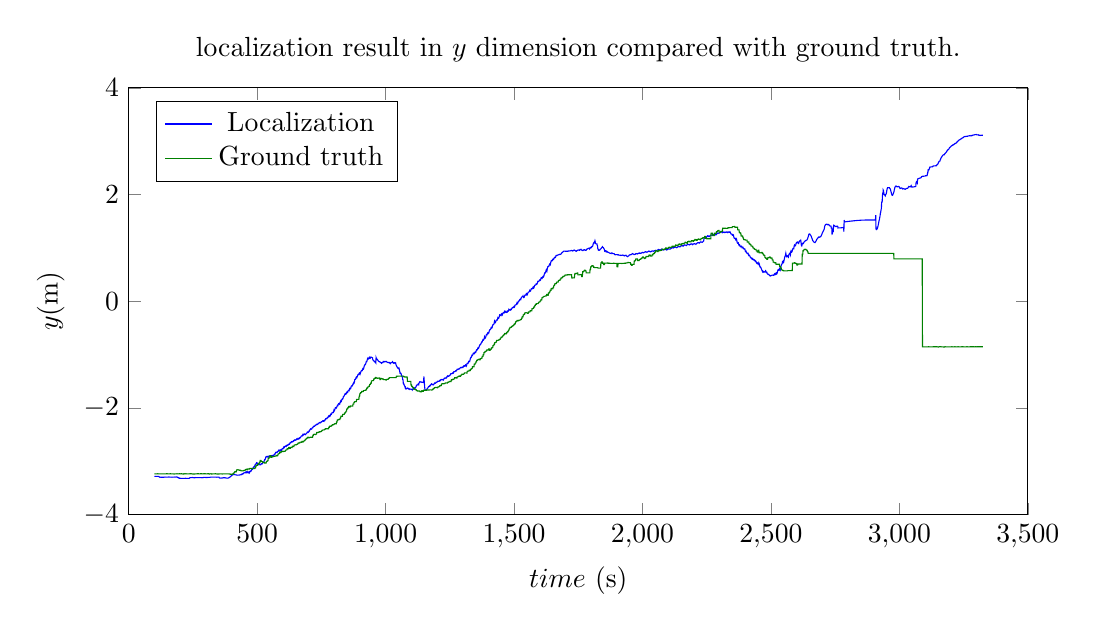
\begin{tikzpicture}

\begin{axis}[
title={localization result in $y$ dimension compared with ground truth.},
xlabel={$time$ (s)},
ylabel={$y$(m)},
xmin=0, xmax=3500,
ymin=-4, ymax=4,
axis on top,
width=13cm,
height=7cm,
legend style={at={(0.03,0.97)}, anchor=north west},
legend entries={{Localization},{Ground truth}}
]
\addplot [blue]
coordinates {
(100,-3.28373563014756)
(101,-3.28492230771622)
(102,-3.28386246980131)
(103,-3.28398329600905)
(104,-3.28391778369171)
(105,-3.28362336997566)
(106,-3.28429983316008)
(107,-3.28476682145083)
(108,-3.28463211082766)
(109,-3.28382919916831)
(110,-3.28486161945998)
(111,-3.28513044511402)
(112,-3.28477786069406)
(113,-3.28513656205148)
(114,-3.28485998372372)
(115,-3.28563984154042)
(116,-3.28733762032329)
(117,-3.2887136596534)
(118,-3.28993030091554)
(119,-3.29498612687579)
(120,-3.29914619639249)
(121,-3.3001108067818)
(122,-3.3017884503071)
(123,-3.30076218841195)
(124,-3.30049153490158)
(125,-3.29990416067345)
(126,-3.3002953007501)
(127,-3.30056763651624)
(128,-3.30075569978134)
(129,-3.30031146133494)
(130,-3.30019428634098)
(131,-3.30057495132558)
(132,-3.30010474944828)
(133,-3.30063366379804)
(134,-3.30089087910721)
(135,-3.30065293325097)
(136,-3.30059280469415)
(137,-3.30045200838736)
(138,-3.30016251616821)
(139,-3.2997260718223)
(140,-3.29989770804456)
(141,-3.29732059018534)
(142,-3.29786742008758)
(143,-3.29874218142786)
(144,-3.2983808048857)
(145,-3.29829276915496)
(146,-3.2981698917737)
(147,-3.29874284146537)
(148,-3.29875532392994)
(149,-3.29898737618896)
(150,-3.29954793259703)
(151,-3.29899938185838)
(152,-3.29836935881977)
(153,-3.29860373424471)
(154,-3.29787171117675)
(155,-3.29713573008045)
(156,-3.29755884232656)
(157,-3.29751563020033)
(158,-3.29765404827603)
(159,-3.29818575185115)
(160,-3.2979654435575)
(161,-3.29801880028028)
(162,-3.29804353859903)
(163,-3.29839316995916)
(164,-3.2983378785061)
(165,-3.29886308468231)
(166,-3.29931784851846)
(167,-3.29959443244767)
(168,-3.30058335846364)
(169,-3.30012439254255)
(170,-3.30031373381272)
(171,-3.29979197386105)
(172,-3.30009224637297)
(173,-3.2999457836919)
(174,-3.29953455412337)
(175,-3.30001807707617)
(176,-3.29917074232039)
(177,-3.29799068985185)
(178,-3.29774082796412)
(179,-3.29927646686511)
(180,-3.29992096366789)
(181,-3.2984676522639)
(182,-3.29859365679411)
(183,-3.29743249773277)
(184,-3.29698627581002)
(185,-3.29695789885195)
(186,-3.29657978337326)
(187,-3.29644037286159)
(188,-3.29678623595348)
(189,-3.2978760921488)
(190,-3.3036275506021)
(191,-3.30734352689617)
(192,-3.30505015581506)
(193,-3.30762664512767)
(194,-3.31107366318989)
(195,-3.31056333803184)
(196,-3.32070380846469)
(197,-3.32094752177084)
(198,-3.32134662751814)
(199,-3.32078107396486)
(200,-3.32052970984211)
(201,-3.32241517821419)
(202,-3.32269412355379)
(203,-3.32309488929064)
(204,-3.32272209673572)
(205,-3.32256030557107)
(206,-3.32315849824371)
(207,-3.32247261772998)
(208,-3.32182261360191)
(209,-3.32191411473343)
(210,-3.32261955276241)
(211,-3.32236355413901)
(212,-3.32205502847342)
(213,-3.32213061388245)
(214,-3.32185851796465)
(215,-3.32224157090229)
(216,-3.32174926044524)
(217,-3.32156821438931)
(218,-3.32153696564939)
(219,-3.32137408127424)
(220,-3.32104381723515)
(221,-3.32110087831738)
(222,-3.32180644820212)
(223,-3.32140690174464)
(224,-3.32145354244975)
(225,-3.32169622830789)
(226,-3.32185978489083)
(227,-3.32181102116302)
(228,-3.32173135616015)
(229,-3.32155788450333)
(230,-3.32149841884099)
(231,-3.32146726484131)
(232,-3.3212781342411)
(233,-3.32126831879757)
(234,-3.32126218524369)
(235,-3.32122909010282)
(236,-3.32046609602456)
(237,-3.31583582135849)
(238,-3.31394150170169)
(239,-3.3092820194197)
(240,-3.30847924638918)
(241,-3.30851718298541)
(242,-3.30867905594209)
(243,-3.30890392712484)
(244,-3.30908003645677)
(245,-3.30861631402263)
(246,-3.3073185300222)
(247,-3.30672797978065)
(248,-3.30680311948149)
(249,-3.3068118142519)
(250,-3.30768172460249)
(251,-3.30780357488889)
(252,-3.30826469280497)
(253,-3.31026182322269)
(254,-3.31093147821215)
(255,-3.31033225894545)
(256,-3.31025351663501)
(257,-3.31097489854765)
(258,-3.30968531432301)
(259,-3.30780079569612)
(260,-3.30667913352177)
(261,-3.3078377910514)
(262,-3.30765416781818)
(263,-3.30818476250195)
(264,-3.30860022844145)
(265,-3.30854950820597)
(266,-3.30872748178811)
(267,-3.30856884936998)
(268,-3.30871773557413)
(269,-3.30773921209644)
(270,-3.30801745323834)
(271,-3.30760834237385)
(272,-3.30765879898259)
(273,-3.30811861121126)
(274,-3.30816744409151)
(275,-3.30714842715657)
(276,-3.30844686498721)
(277,-3.30883460130435)
(278,-3.30895606737875)
(279,-3.30903613580714)
(280,-3.30884975179607)
(281,-3.30905305141041)
(282,-3.30911748141606)
(283,-3.3095292825093)
(284,-3.30973175674683)
(285,-3.30973327979051)
(286,-3.31011650755606)
(287,-3.30947356821083)
(288,-3.3090154296707)
(289,-3.30714828419511)
(290,-3.30550764351308)
(291,-3.30489806897107)
(292,-3.30545437118293)
(293,-3.3037478235034)
(294,-3.30421104945729)
(295,-3.30445060332225)
(296,-3.30418045483147)
(297,-3.30453657575351)
(298,-3.30474318310659)
(299,-3.30601404229987)
(300,-3.30586283967699)
(301,-3.30604808096801)
(302,-3.30609165744731)
(303,-3.30605254472306)
(304,-3.3055493874214)
(305,-3.30513177028146)
(306,-3.30513360308008)
(307,-3.30518106249268)
(308,-3.30489780838666)
(309,-3.30483141419658)
(310,-3.3050851060641)
(311,-3.30478131999644)
(312,-3.30462118754967)
(313,-3.30464438534232)
(314,-3.30452219646808)
(315,-3.30397350118913)
(316,-3.3030309604767)
(317,-3.30125414688654)
(318,-3.29943813487013)
(319,-3.29897035085107)
(320,-3.29911655217309)
(321,-3.29929802546983)
(322,-3.2998952254303)
(323,-3.29946069843605)
(324,-3.2993220347501)
(325,-3.29904613016921)
(326,-3.29919057023946)
(327,-3.29915529993757)
(328,-3.29945305360404)
(329,-3.29970984550944)
(330,-3.29993575666846)
(331,-3.29928730125469)
(332,-3.29900911065966)
(333,-3.29917113976623)
(334,-3.29871195310491)
(335,-3.29869330640874)
(336,-3.29960045070711)
(337,-3.29844278434344)
(338,-3.29838369108826)
(339,-3.29900792930758)
(340,-3.2994807591825)
(341,-3.2995898553239)
(342,-3.30025503975673)
(343,-3.30046201418094)
(344,-3.30038159948878)
(345,-3.29956788515223)
(346,-3.29966743509968)
(347,-3.29966105152303)
(348,-3.29981954952737)
(349,-3.30008166522634)
(350,-3.29980235083838)
(351,-3.29969879042649)
(352,-3.30253107740923)
(353,-3.31444951141799)
(354,-3.31610146886765)
(355,-3.31651835247705)
(356,-3.31675691268452)
(357,-3.31630928248324)
(358,-3.31678813956076)
(359,-3.31650478559663)
(360,-3.31659254448726)
(361,-3.31639940869707)
(362,-3.31615987159038)
(363,-3.31485604818163)
(364,-3.31630081637445)
(365,-3.3135276045864)
(366,-3.31295965264087)
(367,-3.31150798073355)
(368,-3.3112791538552)
(369,-3.31164649662435)
(370,-3.31170798113191)
(371,-3.31203099219009)
(372,-3.3096870064652)
(373,-3.31126311441005)
(374,-3.31098127058406)
(375,-3.31014641114501)
(376,-3.31212691556195)
(377,-3.31373256871633)
(378,-3.31540463705027)
(379,-3.31607932810082)
(380,-3.316044163086)
(381,-3.31791437404908)
(382,-3.31772508118009)
(383,-3.31824902474011)
(384,-3.31769414121628)
(385,-3.3190663807055)
(386,-3.31823298416894)
(387,-3.31692699645929)
(388,-3.31499817279452)
(389,-3.31348700302812)
(390,-3.31117797040267)
(391,-3.30950220055091)
(392,-3.30649888522819)
(393,-3.30226657370048)
(394,-3.29925277819554)
(395,-3.29368136412155)
(396,-3.28953951452551)
(397,-3.28432516064583)
(398,-3.28064339728327)
(399,-3.2769197911025)
(400,-3.27408304418368)
(401,-3.2680247380069)
(402,-3.26533895097901)
(403,-3.26167195343433)
(404,-3.25899559425433)
(405,-3.25604240375685)
(406,-3.25418323351613)
(407,-3.25140076247459)
(408,-3.24916212082832)
(409,-3.24885034870238)
(410,-3.24865551500496)
(411,-3.24853975415989)
(412,-3.25104121879551)
(413,-3.25229515449613)
(414,-3.25497629724084)
(415,-3.25587017532564)
(416,-3.25605782164379)
(417,-3.25573779028863)
(418,-3.25710190455658)
(419,-3.25862402656787)
(420,-3.25917112035686)
(421,-3.26079823630054)
(422,-3.26119470753335)
(423,-3.26233048084821)
(424,-3.26277404532241)
(425,-3.26104165248047)
(426,-3.26132867432175)
(427,-3.26031719165324)
(428,-3.26041746480077)
(429,-3.26003026765324)
(430,-3.26049379578288)
(431,-3.26023238353274)
(432,-3.25901670201309)
(433,-3.25743716887393)
(434,-3.25708894013329)
(435,-3.25511122153531)
(436,-3.25304675610768)
(437,-3.25110900602159)
(438,-3.2474581218846)
(439,-3.25089426923954)
(440,-3.25292773129907)
(441,-3.24647288822237)
(442,-3.23821231745039)
(443,-3.23595304200447)
(444,-3.2370770653841)
(445,-3.23908800274305)
(446,-3.23201298285807)
(447,-3.22629314346229)
(448,-3.22092527292883)
(449,-3.21837051934815)
(450,-3.21790995500544)
(451,-3.22000930694123)
(452,-3.22010586302618)
(453,-3.21656985156713)
(454,-3.21204091879393)
(455,-3.20357589681559)
(456,-3.20348641210827)
(457,-3.21514350992742)
(458,-3.2106203356622)
(459,-3.20218516154546)
(460,-3.20890824671889)
(461,-3.2014033731129)
(462,-3.1989036858734)
(463,-3.20267921565234)
(464,-3.21701780548973)
(465,-3.22041094560847)
(466,-3.21086083351888)
(467,-3.20350861108029)
(468,-3.2006635054474)
(469,-3.20536509380495)
(470,-3.21620355234817)
(471,-3.20567942072877)
(472,-3.19362649161377)
(473,-3.18512423592749)
(474,-3.18542102570307)
(475,-3.18876782443506)
(476,-3.18957265202443)
(477,-3.17860268240725)
(478,-3.16710236233767)
(479,-3.16005057970496)
(480,-3.15071820509059)
(481,-3.15449864224686)
(482,-3.15113703606416)
(483,-3.13417055046541)
(484,-3.128668845568)
(485,-3.11898720327145)
(486,-3.10961328118607)
(487,-3.11142727599415)
(488,-3.112233879485)
(489,-3.11032607065127)
(490,-3.09961934786656)
(491,-3.07994143533651)
(492,-3.06909401408214)
(493,-3.06164403026938)
(494,-3.05761294847042)
(495,-3.05937969837833)
(496,-3.04689187977827)
(497,-3.03582647138694)
(498,-3.0257670116449)
(499,-3.02684850860111)
(500,-3.03372776549064)
(501,-3.04230842187948)
(502,-3.05033416878945)
(503,-3.05394665599606)
(504,-3.05088965128063)
(505,-3.050827880875)
(506,-3.0555543797185)
(507,-3.06588677984629)
(508,-3.0605623223057)
(509,-3.06380991718499)
(510,-3.06041043163084)
(511,-3.05808459738513)
(512,-3.0621212677826)
(513,-3.06741598501435)
(514,-3.06680550607832)
(515,-3.05801477751549)
(516,-3.05094556589967)
(517,-3.04645767691687)
(518,-3.04490111637006)
(519,-3.04572332347884)
(520,-3.04948659311463)
(521,-3.04311101342264)
(522,-3.02896326392051)
(523,-3.02070538600724)
(524,-3.02157563330746)
(525,-3.01969148077721)
(526,-3.01007913715842)
(527,-3.00078426219944)
(528,-2.98678232103838)
(529,-2.974425510838)
(530,-2.97599464887129)
(531,-2.96990453005554)
(532,-2.95595626694452)
(533,-2.93640715558507)
(534,-2.92246203926447)
(535,-2.91352272309745)
(536,-2.91220711950927)
(537,-2.91440153556229)
(538,-2.92081352384199)
(539,-2.92265241123571)
(540,-2.91877617818976)
(541,-2.91440019871579)
(542,-2.90822201156525)
(543,-2.91048418983423)
(544,-2.91215586389424)
(545,-2.9216674014427)
(546,-2.90969800236326)
(547,-2.90297451777322)
(548,-2.90173890997339)
(549,-2.90158805534682)
(550,-2.90778626863688)
(551,-2.91101981734521)
(552,-2.90972258743147)
(553,-2.9067034826143)
(554,-2.90018522687148)
(555,-2.89781048200985)
(556,-2.91144035785073)
(557,-2.90177115307071)
(558,-2.89801778710748)
(559,-2.89665911336903)
(560,-2.89228650356798)
(561,-2.89167710562095)
(562,-2.89099575175154)
(563,-2.90469827763031)
(564,-2.90204869032252)
(565,-2.89161822488808)
(566,-2.87493400770081)
(567,-2.86974288546506)
(568,-2.870640570797)
(569,-2.872004917613)
(570,-2.85924634153321)
(571,-2.84701283596321)
(572,-2.83621176588402)
(573,-2.83041164708854)
(574,-2.83035228429723)
(575,-2.83257415455137)
(576,-2.83691177267751)
(577,-2.83878987451925)
(578,-2.83481507107211)
(579,-2.82391773973941)
(580,-2.81917034317777)
(581,-2.82037176702431)
(582,-2.81162056163268)
(583,-2.8034817071823)
(584,-2.79432564331602)
(585,-2.78929354155211)
(586,-2.7907083875609)
(587,-2.7946196946919)
(588,-2.80562699430867)
(589,-2.80392887058263)
(590,-2.79856471147947)
(591,-2.7895334664442)
(592,-2.7866045327928)
(593,-2.78611237788393)
(594,-2.79744697156653)
(595,-2.79511762589867)
(596,-2.78135727275733)
(597,-2.77069633832599)
(598,-2.76573131819575)
(599,-2.76406376525094)
(600,-2.76699780242596)
(601,-2.76651453659723)
(602,-2.75529308943711)
(603,-2.74186880867495)
(604,-2.73322124953682)
(605,-2.73905296878829)
(606,-2.74339380189973)
(607,-2.73130614333929)
(608,-2.72540996333361)
(609,-2.71802245030585)
(610,-2.71303034854947)
(611,-2.71345757715466)
(612,-2.71671806209748)
(613,-2.72331182338477)
(614,-2.71657471624266)
(615,-2.70559737034262)
(616,-2.69919554080109)
(617,-2.69531524446119)
(618,-2.69790920840165)
(619,-2.70451766723545)
(620,-2.70092036719067)
(621,-2.6949790738503)
(622,-2.68629643764642)
(623,-2.68243633755179)
(624,-2.6795577641367)
(625,-2.68321099631439)
(626,-2.68239682943904)
(627,-2.67163702317256)
(628,-2.65621634598841)
(629,-2.65110255573973)
(630,-2.65518282122833)
(631,-2.65448806202352)
(632,-2.64726353959058)
(633,-2.64348823707611)
(634,-2.63211103492517)
(635,-2.63113197519762)
(636,-2.63255000306473)
(637,-2.63944940044707)
(638,-2.63823882389015)
(639,-2.63455825938871)
(640,-2.62588302449729)
(641,-2.61865321682046)
(642,-2.61383135862827)
(643,-2.61948757089606)
(644,-2.61309625207396)
(645,-2.61032333851616)
(646,-2.60381375523394)
(647,-2.59808247983135)
(648,-2.60079828854277)
(649,-2.60519501304817)
(650,-2.6078382973281)
(651,-2.60288641803634)
(652,-2.60047029094142)
(653,-2.59150913326472)
(654,-2.58497174953442)
(655,-2.59181289149094)
(656,-2.5892283134248)
(657,-2.58696277573592)
(658,-2.57665488549127)
(659,-2.57048328010474)
(660,-2.57051481534392)
(661,-2.57296760092142)
(662,-2.58377344959103)
(663,-2.57904249259819)
(664,-2.57475036376176)
(665,-2.56534340307183)
(666,-2.55728831445758)
(667,-2.55599573499553)
(668,-2.5600523245021)
(669,-2.55218906272325)
(670,-2.54460780544897)
(671,-2.53484272569417)
(672,-2.52806177678135)
(673,-2.52503516372903)
(674,-2.52633977591243)
(675,-2.52701960575368)
(676,-2.52048163130383)
(677,-2.50881057486672)
(678,-2.50022281441234)
(679,-2.51233094158007)
(680,-2.50602159840249)
(681,-2.49923894793913)
(682,-2.49662505186045)
(683,-2.49265980649762)
(684,-2.48905485341188)
(685,-2.49084271157103)
(686,-2.49649506857049)
(687,-2.50364458906016)
(688,-2.50001687775765)
(689,-2.495023583936)
(690,-2.48779624301219)
(691,-2.48379466571196)
(692,-2.48296029953126)
(693,-2.47798327621303)
(694,-2.46405495190867)
(695,-2.45475844527927)
(696,-2.44965835534358)
(697,-2.44951923162479)
(698,-2.45143700818218)
(699,-2.45712326238497)
(700,-2.45269334930628)
(701,-2.44765442434961)
(702,-2.43441995666305)
(703,-2.42739829470424)
(704,-2.43048152764763)
(705,-2.41728336480209)
(706,-2.40742779341483)
(707,-2.39850647527472)
(708,-2.39242116140148)
(709,-2.39283388551163)
(710,-2.40097146922209)
(711,-2.40054562008356)
(712,-2.39949259773442)
(713,-2.39213025921629)
(714,-2.37662658858984)
(715,-2.37017199153763)
(716,-2.36763560895299)
(717,-2.3696891230863)
(718,-2.36207394904938)
(719,-2.35057821675788)
(720,-2.34553455835464)
(721,-2.34581206480265)
(722,-2.34725755023966)
(723,-2.34669725897365)
(724,-2.34346250974079)
(725,-2.33711766013422)
(726,-2.32442109587211)
(727,-2.32461976318636)
(728,-2.32658159743052)
(729,-2.32067990945133)
(730,-2.3189025760526)
(731,-2.3121896955946)
(732,-2.30611740649325)
(733,-2.30644643185008)
(734,-2.30770200369828)
(735,-2.31134906484231)
(736,-2.306336470639)
(737,-2.29827090432122)
(738,-2.28901807375563)
(739,-2.29038940170497)
(740,-2.29177199048869)
(741,-2.28514938596084)
(742,-2.28216112492015)
(743,-2.27517145718926)
(744,-2.27306708769452)
(745,-2.27342652424311)
(746,-2.28101803896334)
(747,-2.27820200382418)
(748,-2.27504065527056)
(749,-2.2674173914183)
(750,-2.2616428798141)
(751,-2.26314752524599)
(752,-2.2615226720624)
(753,-2.25464599893591)
(754,-2.2491631624411)
(755,-2.24308139217796)
(756,-2.24241381427936)
(757,-2.24126728294244)
(758,-2.25102159022242)
(759,-2.25305309753892)
(760,-2.25418142356669)
(761,-2.24106110140202)
(762,-2.23163308231896)
(763,-2.22863818897634)
(764,-2.23332679508739)
(765,-2.22231558387598)
(766,-2.21528730575897)
(767,-2.20259280743824)
(768,-2.20004809011737)
(769,-2.19806012255426)
(770,-2.20309821348713)
(771,-2.20389586838618)
(772,-2.19957178181678)
(773,-2.18824061291064)
(774,-2.17715155239296)
(775,-2.17580726438513)
(776,-2.1785504407842)
(777,-2.1704818172471)
(778,-2.16157775694697)
(779,-2.14868615333268)
(780,-2.14475034588636)
(781,-2.142523331389)
(782,-2.1477325135365)
(783,-2.16011271385171)
(784,-2.15477920159158)
(785,-2.1415286289647)
(786,-2.12391571843177)
(787,-2.11434925550883)
(788,-2.1150599764029)
(789,-2.1201640310148)
(790,-2.11123725340703)
(791,-2.09810415037321)
(792,-2.08776299555234)
(793,-2.08379918946932)
(794,-2.08394175992056)
(795,-2.08913476289248)
(796,-2.09014021422613)
(797,-2.082678431209)
(798,-2.06003989242907)
(799,-2.04186772739833)
(800,-2.04974888838537)
(801,-2.05344857950634)
(802,-2.0327689801382)
(803,-2.02185358530105)
(804,-2.00130538195437)
(805,-1.9971808712642)
(806,-1.99476562710514)
(807,-1.99637838025653)
(808,-2.00470570603191)
(809,-1.99962738079842)
(810,-1.98264244764551)
(811,-1.96981232321236)
(812,-1.95878984051991)
(813,-1.964459879008)
(814,-1.96299260543691)
(815,-1.94688333769741)
(816,-1.9328508692545)
(817,-1.92144864275699)
(818,-1.91741561786116)
(819,-1.91563227269427)
(820,-1.92823002508557)
(821,-1.93240780256201)
(822,-1.91639468132516)
(823,-1.89622749853232)
(824,-1.88585856159508)
(825,-1.87511140868129)
(826,-1.89029076877177)
(827,-1.88549964340598)
(828,-1.8740329310597)
(829,-1.856320455647)
(830,-1.84218273023355)
(831,-1.83455158383981)
(832,-1.82993563472988)
(833,-1.83350574458012)
(834,-1.82555219129037)
(835,-1.80455681403745)
(836,-1.78485896319793)
(837,-1.78291306126801)
(838,-1.78100555140518)
(839,-1.77424388751306)
(840,-1.76335004072655)
(841,-1.75012146158004)
(842,-1.73877299850015)
(843,-1.73271277738317)
(844,-1.73583361452297)
(845,-1.74552502896907)
(846,-1.74249600808529)
(847,-1.73067419759379)
(848,-1.71177064331097)
(849,-1.70627042040939)
(850,-1.70199756624491)
(851,-1.71424265474494)
(852,-1.71047355718165)
(853,-1.70046700870345)
(854,-1.68083685938712)
(855,-1.67427373896912)
(856,-1.67156096577922)
(857,-1.66861831327813)
(858,-1.67463812849032)
(859,-1.65869580885596)
(860,-1.64036336513738)
(861,-1.62955392304198)
(862,-1.62939687715047)
(863,-1.64301882413009)
(864,-1.63894964086302)
(865,-1.61983014180198)
(866,-1.60185496798006)
(867,-1.59082958987085)
(868,-1.58725367615238)
(869,-1.58418655771428)
(870,-1.58858375960354)
(871,-1.58125300094115)
(872,-1.56972849938579)
(873,-1.55074966318995)
(874,-1.54565941062308)
(875,-1.53540527758547)
(876,-1.54637478663565)
(877,-1.54094083715599)
(878,-1.52305587140664)
(879,-1.50634295927458)
(880,-1.4699484623982)
(881,-1.4682226310468)
(882,-1.46307170549615)
(883,-1.46355729605403)
(884,-1.45121980380886)
(885,-1.4275376407533)
(886,-1.42181022433074)
(887,-1.4293987224795)
(888,-1.43389165167354)
(889,-1.42172120744298)
(890,-1.41193881412267)
(891,-1.3942489328188)
(892,-1.38201135693824)
(893,-1.37559711875755)
(894,-1.37119521403491)
(895,-1.37568349831071)
(896,-1.37762976500004)
(897,-1.36516697087643)
(898,-1.34461110556211)
(899,-1.34226008494446)
(900,-1.3515332735784)
(901,-1.36375944822588)
(902,-1.34934037422984)
(903,-1.33551689797703)
(904,-1.31995381023916)
(905,-1.30688599604502)
(906,-1.30370058584571)
(907,-1.29993371262826)
(908,-1.30495690212268)
(909,-1.30343715707377)
(910,-1.28600139079484)
(911,-1.27045396399788)
(912,-1.26002140273879)
(913,-1.26167596826667)
(914,-1.26796163589353)
(915,-1.25260647916231)
(916,-1.23242829136482)
(917,-1.21741197621808)
(918,-1.20028964913554)
(919,-1.19612968538511)
(920,-1.18805538699293)
(921,-1.18989106949806)
(922,-1.18258640404165)
(923,-1.16617513291668)
(924,-1.1450376485048)
(925,-1.13019518982188)
(926,-1.13137948598048)
(927,-1.13113506105657)
(928,-1.11268048865474)
(929,-1.09101473382203)
(930,-1.07551687739282)
(931,-1.06683541542256)
(932,-1.07823362504738)
(933,-1.08023706974161)
(934,-1.08440333158781)
(935,-1.07975436810748)
(936,-1.06966435087475)
(937,-1.05117797265085)
(938,-1.04813960553253)
(939,-1.06573560328465)
(940,-1.0702967109262)
(941,-1.06432316305068)
(942,-1.05510513890875)
(943,-1.05107737061875)
(944,-1.05132567089564)
(945,-1.05045162671055)
(946,-1.05296382777485)
(947,-1.05649832635401)
(948,-1.05917611029143)
(949,-1.06146333061828)
(950,-1.09120556424802)
(951,-1.10209236342678)
(952,-1.10876955004263)
(953,-1.1177582976796)
(954,-1.11980372073671)
(955,-1.12241479602753)
(956,-1.12298433969417)
(957,-1.12713509732183)
(958,-1.1386662744302)
(959,-1.14273393861384)
(960,-1.14925813414226)
(961,-1.15170267871585)
(962,-1.15867423700547)
(963,-1.05801285663162)
(964,-1.07189508947944)
(965,-1.07315605953511)
(966,-1.08390838511286)
(967,-1.09106504597772)
(968,-1.09499166568971)
(969,-1.10022463616495)
(970,-1.10637293227961)
(971,-1.11790391660328)
(972,-1.12366538537205)
(973,-1.12662626386506)
(974,-1.13157038405462)
(975,-1.13235844686739)
(976,-1.1327625197045)
(977,-1.13471524371631)
(978,-1.13995348476004)
(979,-1.14570373498849)
(980,-1.14615435441951)
(981,-1.15059413693354)
(982,-1.1522813100267)
(983,-1.15437077851301)
(984,-1.16403092895152)
(985,-1.15992233516979)
(986,-1.15241844606064)
(987,-1.15086545045028)
(988,-1.14909041156056)
(989,-1.14985218452373)
(990,-1.15090197797053)
(991,-1.13151511700868)
(992,-1.13453103803145)
(993,-1.13306907935165)
(994,-1.13302835252775)
(995,-1.13006140555021)
(996,-1.13396183063028)
(997,-1.13802325948573)
(998,-1.13439611541944)
(999,-1.1299999131913)
(1000,-1.13107385337684)
(1001,-1.13123138588692)
(1002,-1.13145637934106)
(1003,-1.12931883232864)
(1004,-1.13486345236688)
(1005,-1.14112132235778)
(1006,-1.14425976208436)
(1007,-1.14448317317349)
(1008,-1.14742261334)
(1009,-1.15093760146617)
(1010,-1.14955201055707)
(1011,-1.14971471682831)
(1012,-1.14896240565485)
(1013,-1.15257402036121)
(1014,-1.1488354876245)
(1015,-1.15140402637831)
(1016,-1.15703668204992)
(1017,-1.16364099589044)
(1018,-1.17064444608528)
(1019,-1.16396358935152)
(1020,-1.16144874418286)
(1021,-1.15084519049645)
(1022,-1.15092916716479)
(1023,-1.14963211814055)
(1024,-1.14792975355994)
(1025,-1.14961361689406)
(1026,-1.14987013933461)
(1027,-1.13893256187257)
(1028,-1.14901780328211)
(1029,-1.15324786499275)
(1030,-1.15062010854434)
(1031,-1.16209908827839)
(1032,-1.15925318767418)
(1033,-1.15728334472099)
(1034,-1.15177833545075)
(1035,-1.15142453665831)
(1036,-1.16256506366309)
(1037,-1.16553400733865)
(1038,-1.16437934633034)
(1039,-1.15890414666409)
(1040,-1.18107648260307)
(1041,-1.19774720409827)
(1042,-1.20602283647369)
(1043,-1.21845656096848)
(1044,-1.22888470632962)
(1045,-1.23563198545846)
(1046,-1.24255103130765)
(1047,-1.24570905448516)
(1048,-1.25815739767384)
(1049,-1.2614301843937)
(1050,-1.26349997765781)
(1051,-1.26277393988822)
(1052,-1.25531075032241)
(1053,-1.2733836806965)
(1054,-1.29110032131775)
(1055,-1.31624270441016)
(1056,-1.35021533652075)
(1057,-1.35400155871117)
(1058,-1.35204035741055)
(1059,-1.34855191245899)
(1060,-1.35453526752381)
(1061,-1.37131565304861)
(1062,-1.39552591545348)
(1063,-1.40268302181206)
(1064,-1.40344405045091)
(1065,-1.42198502409208)
(1066,-1.44285577187023)
(1067,-1.47481475919757)
(1068,-1.47912725223243)
(1069,-1.5473783368199)
(1070,-1.5504578130258)
(1071,-1.54991826999385)
(1072,-1.5681525572482)
(1073,-1.57694784020832)
(1074,-1.58811802555658)
(1075,-1.59456745085014)
(1076,-1.61654467622042)
(1077,-1.61145282813543)
(1078,-1.62743219348994)
(1079,-1.64765812889365)
(1080,-1.64718274826471)
(1081,-1.64298193559866)
(1082,-1.63875002942853)
(1083,-1.63620505827139)
(1084,-1.63236691967131)
(1085,-1.62839517654308)
(1086,-1.6261943945537)
(1087,-1.63076507850975)
(1088,-1.6384798305125)
(1089,-1.63993032257478)
(1090,-1.64219143886684)
(1091,-1.65133892520492)
(1092,-1.65485821350498)
(1093,-1.6471940718868)
(1094,-1.64355351134427)
(1095,-1.6482252599811)
(1096,-1.6494572599276)
(1097,-1.64940849258997)
(1098,-1.64952534111495)
(1099,-1.65299377290919)
(1100,-1.65137511503763)
(1101,-1.65468765145429)
(1102,-1.65452800648143)
(1103,-1.65589182214714)
(1104,-1.66538287994356)
(1105,-1.65775009045587)
(1106,-1.64929719348407)
(1107,-1.63894590271578)
(1108,-1.63932854407873)
(1109,-1.64108619872984)
(1110,-1.64060364259425)
(1111,-1.64495226680365)
(1112,-1.6367445131291)
(1113,-1.62866978490395)
(1114,-1.62111777805803)
(1115,-1.62230208741248)
(1116,-1.62716896774855)
(1117,-1.62435220988122)
(1118,-1.60756553500718)
(1119,-1.59801602344474)
(1120,-1.58022885809703)
(1121,-1.57543928761182)
(1122,-1.56944038841732)
(1123,-1.56886188776728)
(1124,-1.57087440242066)
(1125,-1.56793161332808)
(1126,-1.55446904123468)
(1127,-1.55015824312793)
(1128,-1.55441931834958)
(1129,-1.56194182844155)
(1130,-1.54163759866446)
(1131,-1.52679882388371)
(1132,-1.51703568157509)
(1133,-1.51048521733843)
(1134,-1.50910264483857)
(1135,-1.51149978789473)
(1136,-1.51748435830636)
(1137,-1.51693177686866)
(1138,-1.51637166493041)
(1139,-1.51504813189553)
(1140,-1.51806535488527)
(1141,-1.52148912383767)
(1142,-1.51963378819286)
(1143,-1.52257549703979)
(1144,-1.52136956968251)
(1145,-1.52080456844403)
(1146,-1.52333800958359)
(1147,-1.52481376431983)
(1148,-1.5251803130672)
(1149,-1.41196746238537)
(1150,-1.47400187370194)
(1151,-1.53465464944134)
(1152,-1.59892470305142)
(1153,-1.65389043196149)
(1154,-1.66879563106712)
(1155,-1.66910471878407)
(1156,-1.67170109241249)
(1157,-1.66873987296113)
(1158,-1.66708544128789)
(1159,-1.65921556333803)
(1160,-1.65694998025395)
(1161,-1.64735299025083)
(1162,-1.64286623375682)
(1163,-1.63592225332756)
(1164,-1.62962770073789)
(1165,-1.62240114044341)
(1166,-1.61375692522157)
(1167,-1.60484478548825)
(1168,-1.59927063333982)
(1169,-1.59925256440206)
(1170,-1.60052489111468)
(1171,-1.59601499560793)
(1172,-1.58188550059732)
(1173,-1.57596460802285)
(1174,-1.57376130227671)
(1175,-1.57837761877898)
(1176,-1.56748379591379)
(1177,-1.55718364445349)
(1178,-1.5535337640677)
(1179,-1.54944202015581)
(1180,-1.55340946779665)
(1181,-1.56149147298808)
(1182,-1.56497312226501)
(1183,-1.56637488183517)
(1184,-1.56495166302921)
(1185,-1.55893375716555)
(1186,-1.55919880595657)
(1187,-1.56561718493456)
(1188,-1.55711294253999)
(1189,-1.54853239872397)
(1190,-1.53796014769172)
(1191,-1.53168880386746)
(1192,-1.53270680410063)
(1193,-1.53728391420396)
(1194,-1.53926018287921)
(1195,-1.5339771632563)
(1196,-1.52666129748796)
(1197,-1.51865970862429)
(1198,-1.52215489083149)
(1199,-1.52309843521294)
(1200,-1.51931491750701)
(1201,-1.5121246465266)
(1202,-1.50832827622938)
(1203,-1.50106471910447)
(1204,-1.49955280491047)
(1205,-1.50161006452966)
(1206,-1.50280565086599)
(1207,-1.50181340048451)
(1208,-1.50194544744897)
(1209,-1.49711619006579)
(1210,-1.49118880144586)
(1211,-1.48611782901831)
(1212,-1.49463715185368)
(1213,-1.49393397046071)
(1214,-1.4826168031582)
(1215,-1.47125514911846)
(1216,-1.46901726332968)
(1217,-1.46860235376048)
(1218,-1.46997601510181)
(1219,-1.47386394341175)
(1220,-1.47473643168994)
(1221,-1.47565306454728)
(1222,-1.47131005413802)
(1223,-1.46670594711992)
(1224,-1.47140755758218)
(1225,-1.47664159674187)
(1226,-1.46392152373694)
(1227,-1.45843314455853)
(1228,-1.44776735660708)
(1229,-1.44209322705083)
(1230,-1.4413582267694)
(1231,-1.44369229099566)
(1232,-1.44509374327134)
(1233,-1.44376460491369)
(1234,-1.44213902957543)
(1235,-1.43525803673139)
(1236,-1.43074956995248)
(1237,-1.43822748933536)
(1238,-1.43299289951999)
(1239,-1.42006078143999)
(1240,-1.41081720228969)
(1241,-1.40137599440897)
(1242,-1.39907620640745)
(1243,-1.39978432483309)
(1244,-1.40875250825786)
(1245,-1.40709921550934)
(1246,-1.40736450707349)
(1247,-1.39991662640251)
(1248,-1.39374690113249)
(1249,-1.39188261862863)
(1250,-1.3925856577885)
(1251,-1.38583962685598)
(1252,-1.37686602009391)
(1253,-1.36471560969546)
(1254,-1.358788334041)
(1255,-1.35865060669787)
(1256,-1.3618850523476)
(1257,-1.3628465334983)
(1258,-1.36036191496753)
(1259,-1.35566437274943)
(1260,-1.34779663312568)
(1261,-1.3451651390725)
(1262,-1.35262760861727)
(1263,-1.35182110560664)
(1264,-1.33890388940015)
(1265,-1.32901189033026)
(1266,-1.32038091931202)
(1267,-1.32045626616732)
(1268,-1.31974384608658)
(1269,-1.32127076473017)
(1270,-1.31659702069411)
(1271,-1.31573986996889)
(1272,-1.31066697146693)
(1273,-1.30489794739988)
(1274,-1.30550712472683)
(1275,-1.30845832182961)
(1276,-1.30096912553862)
(1277,-1.29196267403271)
(1278,-1.28135043590363)
(1279,-1.27400924883113)
(1280,-1.27446761975697)
(1281,-1.27861041730168)
(1282,-1.28042217168778)
(1283,-1.27818035962924)
(1284,-1.27424767116101)
(1285,-1.26837294819808)
(1286,-1.26606284929167)
(1287,-1.26994076738525)
(1288,-1.2705404988032)
(1289,-1.26368107667899)
(1290,-1.25237414532965)
(1291,-1.24635637538506)
(1292,-1.24154998575939)
(1293,-1.24244909196924)
(1294,-1.24697345071787)
(1295,-1.24749959220844)
(1296,-1.24541064287508)
(1297,-1.24262071896818)
(1298,-1.23439418211138)
(1299,-1.23701361529666)
(1300,-1.24376099809098)
(1301,-1.2448923233872)
(1302,-1.23557612068257)
(1303,-1.22036267644475)
(1304,-1.21555635821645)
(1305,-1.20960179472329)
(1306,-1.20828310646904)
(1307,-1.2129970374832)
(1308,-1.22010899459947)
(1309,-1.21569117208959)
(1310,-1.20243961099452)
(1311,-1.19326094336303)
(1312,-1.19511168863315)
(1313,-1.20776889539088)
(1314,-1.21690801628608)
(1315,-1.20561464938116)
(1316,-1.19155484414642)
(1317,-1.17158793509061)
(1318,-1.16468316902764)
(1319,-1.16472301190392)
(1320,-1.16358051540421)
(1321,-1.16579879689095)
(1322,-1.15430812491831)
(1323,-1.13349320144494)
(1324,-1.12503328389938)
(1325,-1.12626830425588)
(1326,-1.13305723929071)
(1327,-1.13395010773323)
(1328,-1.1153861054422)
(1329,-1.0955289016573)
(1330,-1.07482292206815)
(1331,-1.06365009308816)
(1332,-1.05499927970512)
(1333,-1.05667729083866)
(1334,-1.04674128840571)
(1335,-1.03284015305501)
(1336,-1.01547437488041)
(1337,-1.01894803444111)
(1338,-1.0189559875462)
(1339,-1.00786995753919)
(1340,-0.995281598748217)
(1341,-0.980196600184214)
(1342,-0.972772384663919)
(1343,-0.973797817052048)
(1344,-0.975796031356814)
(1345,-0.984659261395916)
(1346,-0.978712697326831)
(1347,-0.965216724126756)
(1348,-0.955398533269942)
(1349,-0.952269216193591)
(1350,-0.962430655118152)
(1351,-0.960822500859936)
(1352,-0.943404729193942)
(1353,-0.926003807358949)
(1354,-0.912108259630528)
(1355,-0.909097688615069)
(1356,-0.909786945414024)
(1357,-0.91253493631881)
(1358,-0.903744788486569)
(1359,-0.882435746126479)
(1360,-0.872331913752126)
(1361,-0.875364894502452)
(1362,-0.879863647134098)
(1363,-0.869723852268651)
(1364,-0.856170553087143)
(1365,-0.837746963979185)
(1366,-0.826664929250698)
(1367,-0.817169974258413)
(1368,-0.817094677062333)
(1369,-0.817291380735416)
(1370,-0.810570027319719)
(1371,-0.800067891480033)
(1372,-0.782980898166708)
(1373,-0.779626984900207)
(1374,-0.766868525358968)
(1375,-0.769994424667169)
(1376,-0.76453955806214)
(1377,-0.74986858517646)
(1378,-0.729685768696787)
(1379,-0.721457805269684)
(1380,-0.72767974408239)
(1381,-0.72996480181439)
(1382,-0.71804646292041)
(1383,-0.710526269551665)
(1384,-0.694425863053545)
(1385,-0.671393734317058)
(1386,-0.68708165581095)
(1387,-0.694785936426615)
(1388,-0.690043100437922)
(1389,-0.683283926181949)
(1390,-0.667498387050041)
(1391,-0.650995792657143)
(1392,-0.62876592453291)
(1393,-0.625792760535505)
(1394,-0.620708556607181)
(1395,-0.626007331401329)
(1396,-0.611805706218766)
(1397,-0.600652397408685)
(1398,-0.589712693066344)
(1399,-0.587923793234886)
(1400,-0.59572927083533)
(1401,-0.601744436067712)
(1402,-0.590480845914754)
(1403,-0.572745850175161)
(1404,-0.552860078192695)
(1405,-0.537676320904496)
(1406,-0.535817739421908)
(1407,-0.53468964371076)
(1408,-0.533570288545091)
(1409,-0.522948910167387)
(1410,-0.510701695842335)
(1411,-0.489677540417999)
(1412,-0.489486373586741)
(1413,-0.489769210193096)
(1414,-0.498413608681798)
(1415,-0.488649007622393)
(1416,-0.46696627468321)
(1417,-0.452531336445242)
(1418,-0.43994862637799)
(1419,-0.438369076595586)
(1420,-0.437854444450717)
(1421,-0.433954249909051)
(1422,-0.422363825361629)
(1423,-0.401866373490356)
(1424,-0.378879744754742)
(1425,-0.395175709971405)
(1426,-0.405515351996716)
(1427,-0.405586510747495)
(1428,-0.394816490095048)
(1429,-0.381292131680143)
(1430,-0.362653255298498)
(1431,-0.358611753808645)
(1432,-0.353674157932609)
(1433,-0.353999581680311)
(1434,-0.355866908976345)
(1435,-0.349790250461472)
(1436,-0.329268473395638)
(1437,-0.313229864498785)
(1438,-0.323760212138227)
(1439,-0.326450349812044)
(1440,-0.325067288507721)
(1441,-0.314456766146919)
(1442,-0.29425007233006)
(1443,-0.281183478254198)
(1444,-0.257237401569333)
(1445,-0.2603095109141)
(1446,-0.268264932194437)
(1447,-0.269355825692575)
(1448,-0.261156468713459)
(1449,-0.253521166309709)
(1450,-0.243226250671457)
(1451,-0.238615180309873)
(1452,-0.255715638044408)
(1453,-0.266899268812525)
(1454,-0.260692655405311)
(1455,-0.249459205920193)
(1456,-0.228702303999433)
(1457,-0.221034183014668)
(1458,-0.217919752458278)
(1459,-0.216684378275382)
(1460,-0.22188082906357)
(1461,-0.222075112307162)
(1462,-0.202169755868436)
(1463,-0.189242162742377)
(1464,-0.194028938877638)
(1465,-0.202806212365284)
(1466,-0.196037194872665)
(1467,-0.190323102996523)
(1468,-0.187899604243178)
(1469,-0.208661937991065)
(1470,-0.210296116182745)
(1471,-0.210547999263442)
(1472,-0.211319849705423)
(1473,-0.209362662791232)
(1474,-0.196075053236488)
(1475,-0.183244991645322)
(1476,-0.182778589892829)
(1477,-0.179683821118582)
(1478,-0.183774623155962)
(1479,-0.170119596772896)
(1480,-0.154816968087131)
(1481,-0.162985148948004)
(1482,-0.157322079625609)
(1483,-0.159801314650593)
(1484,-0.167486511775174)
(1485,-0.169432799665505)
(1486,-0.16168223181959)
(1487,-0.149392053454751)
(1488,-0.150616466547441)
(1489,-0.157474332536525)
(1490,-0.152118360895444)
(1491,-0.141446881072935)
(1492,-0.130488561637305)
(1493,-0.124466953293879)
(1494,-0.118342505996579)
(1495,-0.11846072549107)
(1496,-0.122888466906373)
(1497,-0.120149191413426)
(1498,-0.113874313452699)
(1499,-0.104229555979066)
(1500,-0.0957322037373483)
(1501,-0.094417032136067)
(1502,-0.105167067854005)
(1503,-0.0930910560328608)
(1504,-0.0756207632259085)
(1505,-0.069425298476564)
(1506,-0.0681498385643019)
(1507,-0.0684628975451859)
(1508,-0.0674770091747643)
(1509,-0.0608697825771846)
(1510,-0.0470196265879131)
(1511,-0.0359438540511642)
(1512,-0.0530187674115769)
(1513,-0.0507528484028165)
(1514,-0.0400916812684797)
(1515,-0.0274763153984872)
(1516,-0.0160218311626451)
(1517,-0.000802453671360694)
(1518,-0.00292007549652292)
(1519,0.00274425306176324)
(1520,0.00525039748579898)
(1521,0.0159963183139944)
(1522,0.0290027690393875)
(1523,0.0348727219426371)
(1524,0.0381437301476142)
(1525,0.0339187671082337)
(1526,0.0290690518634679)
(1527,0.0446286391490132)
(1528,0.062944765528282)
(1529,0.0729034480884883)
(1530,0.0775554383610607)
(1531,0.079840303151731)
(1532,0.0844421199049723)
(1533,0.086061037256546)
(1534,0.0888053222020673)
(1535,0.0991360368067868)
(1536,0.0844556042051198)
(1537,0.0737466005142752)
(1538,0.0665223801883885)
(1539,0.0709476075007236)
(1540,0.0813245032961201)
(1541,0.0923130707164774)
(1542,0.111525971025193)
(1543,0.115553116584763)
(1544,0.116794886146988)
(1545,0.116030032232046)
(1546,0.116279559626418)
(1547,0.13097982394155)
(1548,0.14183671313241)
(1549,0.136058418716248)
(1550,0.128818829530021)
(1551,0.118748224020966)
(1552,0.128337056654241)
(1553,0.140478364986019)
(1554,0.154766120797548)
(1555,0.166293670030601)
(1556,0.169556641963292)
(1557,0.171590446073428)
(1558,0.172701665468309)
(1559,0.179193888641528)
(1560,0.187739159681939)
(1561,0.202003795814504)
(1562,0.193969554178299)
(1563,0.186545714800363)
(1564,0.188013929037331)
(1565,0.202046446848649)
(1566,0.216361993802779)
(1567,0.232440674464503)
(1568,0.237063778731756)
(1569,0.233440509270713)
(1570,0.232939201778234)
(1571,0.233314428961996)
(1572,0.241723035647528)
(1573,0.252862233385955)
(1574,0.26154890444358)
(1575,0.252934960002158)
(1576,0.242794604413489)
(1577,0.247585514725309)
(1578,0.258711117475574)
(1579,0.283895130684854)
(1580,0.294709941773205)
(1581,0.300339040568478)
(1582,0.301336758219728)
(1583,0.301918343981772)
(1584,0.302113855326481)
(1585,0.310619137307975)
(1586,0.324084636382583)
(1587,0.32111481993704)
(1588,0.316015659070457)
(1589,0.317991161215012)
(1590,0.328972969103879)
(1591,0.343322358414617)
(1592,0.36422040299316)
(1593,0.373475841044521)
(1594,0.373995454344376)
(1595,0.373753471624621)
(1596,0.370837904339306)
(1597,0.374267003484958)
(1598,0.381397639055005)
(1599,0.394623372779463)
(1600,0.400106302735215)
(1601,0.395779393349067)
(1602,0.390758615159966)
(1603,0.395905779722152)
(1604,0.415823545431731)
(1605,0.426427291991985)
(1606,0.442335480916513)
(1607,0.439679588204423)
(1608,0.43126288036327)
(1609,0.426626110480857)
(1610,0.432713812689711)
(1611,0.444165655622132)
(1612,0.459923433082805)
(1613,0.467349417261563)
(1614,0.46829616538614)
(1615,0.460173370711913)
(1616,0.469406103346771)
(1617,0.488813052859777)
(1618,0.510629627470436)
(1619,0.525020299841995)
(1620,0.532298873334764)
(1621,0.535343982150309)
(1622,0.532705023814687)
(1623,0.542927022642882)
(1624,0.56286370698749)
(1625,0.586790749144527)
(1626,0.593543374184019)
(1627,0.57901908568134)
(1628,0.567489340519199)
(1629,0.596064432365074)
(1630,0.621223735871196)
(1631,0.639504241088221)
(1632,0.649835000385829)
(1633,0.652748560383004)
(1634,0.655724119670371)
(1635,0.652356664870927)
(1636,0.659341110153225)
(1637,0.676787611764674)
(1638,0.692156592751128)
(1639,0.698418940446109)
(1640,0.693965283044527)
(1641,0.684780625821968)
(1642,0.702649249483814)
(1643,0.728807053602299)
(1644,0.742702356825917)
(1645,0.757576964211148)
(1646,0.764700754205116)
(1647,0.764793232308502)
(1648,0.757909432769292)
(1649,0.759430960420348)
(1650,0.775294644474283)
(1651,0.7875801002983)
(1652,0.789887349393973)
(1653,0.780815951885293)
(1654,0.780038805703693)
(1655,0.80021463469566)
(1656,0.807836388895413)
(1657,0.817511116698514)
(1658,0.820349049994592)
(1659,0.817565406057547)
(1660,0.825493647368999)
(1661,0.8214702883874)
(1662,0.82754642517867)
(1663,0.85136003113266)
(1664,0.857013967525231)
(1665,0.857299779222356)
(1666,0.853736896453516)
(1667,0.853854375939628)
(1668,0.861066660559523)
(1669,0.865068907749195)
(1670,0.865202681371427)
(1671,0.868287756721842)
(1672,0.869147835722493)
(1673,0.870386771178132)
(1674,0.868590471564439)
(1675,0.871536632888082)
(1676,0.876107306798624)
(1677,0.879817018057005)
(1678,0.878521000482223)
(1679,0.875959071418993)
(1680,0.877179588591365)
(1681,0.877919950089755)
(1682,0.88394793421935)
(1683,0.888713566957392)
(1684,0.88832318756114)
(1685,0.897846175685327)
(1686,0.906822851904334)
(1687,0.908853959864534)
(1688,0.914572846586079)
(1689,0.918602045271415)
(1690,0.922172000654089)
(1691,0.928718525174972)
(1692,0.930124073738348)
(1693,0.936678157871966)
(1694,0.937912543286994)
(1695,0.937507285532972)
(1696,0.938135179529343)
(1697,0.938529134464358)
(1698,0.938691828733185)
(1699,0.938590096355005)
(1700,0.935254169624809)
(1701,0.935496460075516)
(1702,0.936448390615242)
(1703,0.936677826734537)
(1704,0.936830616359068)
(1705,0.935869703276775)
(1706,0.935614674152894)
(1707,0.935497175550885)
(1708,0.935660720443891)
(1709,0.93605526877517)
(1710,0.937450847340642)
(1711,0.941270337298825)
(1712,0.941253696691248)
(1713,0.942347207918446)
(1714,0.942315868499167)
(1715,0.942416314324317)
(1716,0.942271892179589)
(1717,0.941833127157991)
(1718,0.942428029810405)
(1719,0.94347318465745)
(1720,0.944984488595767)
(1721,0.94839385376974)
(1722,0.950322373361839)
(1723,0.950201881090921)
(1724,0.949785284600623)
(1725,0.946843280654451)
(1726,0.945299845648782)
(1727,0.946484733572408)
(1728,0.945176784040512)
(1729,0.941128022350634)
(1730,0.94655807800329)
(1731,0.951862505478559)
(1732,0.954501879251041)
(1733,0.953238549394344)
(1734,0.956076311292006)
(1735,0.958829557585846)
(1736,0.954957593886843)
(1737,0.953038088073176)
(1738,0.94708952840798)
(1739,0.94389566217118)
(1740,0.940948387630902)
(1741,0.937014113868425)
(1742,0.935620205626922)
(1743,0.940418497763481)
(1744,0.945895915823194)
(1745,0.948124036435058)
(1746,0.947664267192204)
(1747,0.952140975149401)
(1748,0.958339294846579)
(1749,0.95906269067016)
(1750,0.958508029538125)
(1751,0.957320837656188)
(1752,0.959582133710275)
(1753,0.959476446995341)
(1754,0.954471310255424)
(1755,0.95400448307808)
(1756,0.961088882342973)
(1757,0.968497304725692)
(1758,0.968748867523335)
(1759,0.965797061243738)
(1760,0.96961124307138)
(1761,0.972416634445962)
(1762,0.964938627211204)
(1763,0.960402724031415)
(1764,0.957799503795332)
(1765,0.952332493942717)
(1766,0.949272171356763)
(1767,0.947438645334044)
(1768,0.947525313894742)
(1769,0.954121277744439)
(1770,0.959932052498813)
(1771,0.960207718003078)
(1772,0.959242375452432)
(1773,0.964312833702207)
(1774,0.965802141325221)
(1775,0.962904327059087)
(1776,0.961660111007371)
(1777,0.955092856092659)
(1778,0.95197604806765)
(1779,0.952090832908077)
(1780,0.951650910045145)
(1781,0.958354868769905)
(1782,0.967571439710813)
(1783,0.975264971766405)
(1784,0.978536307742528)
(1785,0.978312828096094)
(1786,0.980689232842556)
(1787,0.985510286307465)
(1788,0.987549243728691)
(1789,0.989354322705686)
(1790,0.990741243688825)
(1791,0.993228287418509)
(1792,0.991312767116628)
(1793,0.984747208792729)
(1794,0.979094827804432)
(1795,0.994638634930776)
(1796,1.00254664673948)
(1797,1.00588823660775)
(1798,1.0009770340275)
(1799,0.998130653827784)
(1800,0.999467781659633)
(1801,1.00974130380176)
(1802,1.02238783755955)
(1803,1.02601648549744)
(1804,1.0220338204786)
(1805,1.02257276658685)
(1806,1.03021033903749)
(1807,1.05024454517051)
(1808,1.06964135340015)
(1809,1.08602349810753)
(1810,1.09257026867909)
(1811,1.0997520348827)
(1812,1.09237338578748)
(1813,1.09093973129591)
(1814,1.11588055970797)
(1815,1.13365054374733)
(1816,1.11631115377495)
(1817,1.08992246329206)
(1818,1.08111761820393)
(1819,1.07491304736018)
(1820,1.07534943809741)
(1821,1.07274708532498)
(1822,1.0720504778707)
(1823,1.07197812910373)
(1824,1.04500863527162)
(1825,1.03728649243709)
(1826,0.987772630429236)
(1827,0.978134694447753)
(1828,0.961842889549269)
(1829,0.963022439270025)
(1830,0.954802698990141)
(1831,0.955682560024556)
(1832,0.955130963663422)
(1833,0.961020454033899)
(1834,0.964182645077993)
(1835,0.964815392471938)
(1836,0.975397045141644)
(1837,0.979424760862892)
(1838,0.983097602592481)
(1839,0.988641491479032)
(1840,0.996121681424171)
(1841,0.998551208125919)
(1842,1.00811231382595)
(1843,1.01355178758196)
(1844,1.02188381720199)
(1845,1.01617329232269)
(1846,1.0089649694628)
(1847,1.00635748531072)
(1848,1.00374760583649)
(1849,0.993952547162764)
(1850,0.981395013970944)
(1851,0.977953346318774)
(1852,0.96258602719849)
(1853,0.940087581138927)
(1854,0.944272762338657)
(1855,0.942737034743918)
(1856,0.945770152649662)
(1857,0.941287053159167)
(1858,0.924814411415206)
(1859,0.925161530222108)
(1860,0.923069461989862)
(1861,0.936411389690364)
(1862,0.933507678981323)
(1863,0.929278042119827)
(1864,0.925865286014897)
(1865,0.917157659118133)
(1866,0.915753784227111)
(1867,0.916019440721023)
(1868,0.914053886195308)
(1869,0.91164792432057)
(1870,0.908541761862492)
(1871,0.904114779524613)
(1872,0.902293927100808)
(1873,0.900399796226949)
(1874,0.898282755075723)
(1875,0.896904529463908)
(1876,0.896254599161261)
(1877,0.89564355979928)
(1878,0.893127721649492)
(1879,0.903628497548782)
(1880,0.903675093714437)
(1881,0.903104188119781)
(1882,0.901447365624806)
(1883,0.901066391066662)
(1884,0.893325611595173)
(1885,0.89271806287297)
(1886,0.892872706542709)
(1887,0.892604558982497)
(1888,0.892359026462203)
(1889,0.891193629953656)
(1890,0.890925739890392)
(1891,0.880175096568164)
(1892,0.872880416687551)
(1893,0.871826476227214)
(1894,0.871518112701371)
(1895,0.871794164026352)
(1896,0.872016854107429)
(1897,0.871992983733592)
(1898,0.87218694652241)
(1899,0.872503137607378)
(1900,0.872567307527406)
(1901,0.872516525871842)
(1902,0.870453674638925)
(1903,0.868215754727486)
(1904,0.872521928376538)
(1905,0.870730870663205)
(1906,0.870196290069937)
(1907,0.864852568259288)
(1908,0.865417013210555)
(1909,0.863518485774759)
(1910,0.863596040366466)
(1911,0.863700786932874)
(1912,0.86187605570008)
(1913,0.861105502338935)
(1914,0.861128598115803)
(1915,0.861253807528878)
(1916,0.857130079237864)
(1917,0.858012192738606)
(1918,0.85961825873272)
(1919,0.860286759881201)
(1920,0.861317621584834)
(1921,0.862288461377192)
(1922,0.863827983465905)
(1923,0.865160620044763)
(1924,0.865337857910649)
(1925,0.861084599820161)
(1926,0.858494741165542)
(1927,0.858731378792676)
(1928,0.85564186181162)
(1929,0.849018504303821)
(1930,0.850203245833365)
(1931,0.855758964706625)
(1932,0.856429087208851)
(1933,0.857679483735707)
(1934,0.857378388562571)
(1935,0.860646444525681)
(1936,0.861179204465606)
(1937,0.855175841304156)
(1938,0.850790622525704)
(1939,0.844389266078418)
(1940,0.841442318592916)
(1941,0.839332880533593)
(1942,0.835417651532321)
(1943,0.838191104475146)
(1944,0.842278410463554)
(1945,0.848253374792407)
(1946,0.850685438864694)
(1947,0.852436245079248)
(1948,0.858935813652917)
(1949,0.867465095993477)
(1950,0.86969478886093)
(1951,0.867846024113565)
(1952,0.867522325113291)
(1953,0.870631775583264)
(1954,0.870511145680987)
(1955,0.870231759434599)
(1956,0.873441522318154)
(1957,0.878283994060853)
(1958,0.882151725145722)
(1959,0.884648349710026)
(1960,0.885865736096736)
(1961,0.891917792560839)
(1962,0.893588626216126)
(1963,0.888986247239282)
(1964,0.884486248041827)
(1965,0.881114348699551)
(1966,0.879853956317966)
(1967,0.873635185432131)
(1968,0.873045700801617)
(1969,0.875793745035911)
(1970,0.880093995451807)
(1971,0.882136022840689)
(1972,0.88093511682667)
(1973,0.886293870779208)
(1974,0.891290440983288)
(1975,0.89348217841898)
(1976,0.891810180328485)
(1977,0.887720135189153)
(1978,0.889011859699064)
(1979,0.888830407864907)
(1980,0.884797827054434)
(1981,0.886579631709118)
(1982,0.890781403079568)
(1983,0.894149353442128)
(1984,0.896005548776033)
(1985,0.897206310720484)
(1986,0.901128630137484)
(1987,0.903475017805561)
(1988,0.90088397407627)
(1989,0.897936231414031)
(1990,0.9022012830211)
(1991,0.900703162245244)
(1992,0.896132214831717)
(1993,0.895522881432362)
(1994,0.899548762362726)
(1995,0.904012948704469)
(1996,0.903737152551307)
(1997,0.903468668157925)
(1998,0.9080339394862)
(1999,0.915496669302604)
(2000,0.91641873174293)
(2001,0.913952590345795)
(2002,0.910680259288942)
(2003,0.909607288419049)
(2004,0.907444721664857)
(2005,0.908709057377794)
(2006,0.911668741866095)
(2007,0.917318156048112)
(2008,0.921317983558827)
(2009,0.921865409782045)
(2010,0.920143140578428)
(2011,0.925967487220773)
(2012,0.928102344244095)
(2013,0.927747355898996)
(2014,0.92539207630937)
(2015,0.924106021568735)
(2016,0.91956119668906)
(2017,0.91659431331106)
(2018,0.918931261469987)
(2019,0.920929227369685)
(2020,0.9260458603643)
(2021,0.928232917181791)
(2022,0.928667712448358)
(2023,0.931680862982106)
(2024,0.935825113295947)
(2025,0.941543088575127)
(2026,0.939163785601369)
(2027,0.932692067805098)
(2028,0.930726888223)
(2029,0.928971134766145)
(2030,0.927386986375188)
(2031,0.925954735479632)
(2032,0.930277379197276)
(2033,0.928969742909938)
(2034,0.933768485568124)
(2035,0.934754784725586)
(2036,0.938102928942608)
(2037,0.942589411413532)
(2038,0.943901309644319)
(2039,0.942511436232442)
(2040,0.939294252850506)
(2041,0.941728200622826)
(2042,0.940573705049041)
(2043,0.937480537486444)
(2044,0.935943314511266)
(2045,0.939731029846073)
(2046,0.944693761268234)
(2047,0.946854138357473)
(2048,0.948318365773473)
(2049,0.950354263531629)
(2050,0.954071159289191)
(2051,0.95352945127323)
(2052,0.95132261971181)
(2053,0.949928347634195)
(2054,0.95219873825502)
(2055,0.949643394152152)
(2056,0.947542242572879)
(2057,0.951348943289006)
(2058,0.955052962016996)
(2059,0.95874850393831)
(2060,0.96158472823491)
(2061,0.964211563062844)
(2062,0.969606000284493)
(2063,0.96965317198688)
(2064,0.967825690553807)
(2065,0.964099676170543)
(2066,0.96394255609221)
(2067,0.963028776629471)
(2068,0.958000976669196)
(2069,0.957313552023385)
(2070,0.962678268842664)
(2071,0.96640950840098)
(2072,0.968736748188237)
(2073,0.971451879685986)
(2074,0.97457051455654)
(2075,0.977409392702394)
(2076,0.976006819607994)
(2077,0.975437031568731)
(2078,0.969980202865258)
(2079,0.969959437531948)
(2080,0.963470041249918)
(2081,0.959178415411798)
(2082,0.960582039767351)
(2083,0.965531885687837)
(2084,0.967675922589431)
(2085,0.967440069275479)
(2086,0.970277831580579)
(2087,0.971759158689763)
(2088,0.972875012674992)
(2089,0.972154405642652)
(2090,0.97071749115499)
(2091,0.967313508495142)
(2092,0.966620629178414)
(2093,0.964496199196906)
(2094,0.959358426723007)
(2095,0.959047822680277)
(2096,0.964867941581857)
(2097,0.968928807039847)
(2098,0.972175780997601)
(2099,0.975873691949377)
(2100,0.979282419268424)
(2101,0.982020765903907)
(2102,0.982663332214294)
(2103,0.981623498062556)
(2104,0.978278037535986)
(2105,0.978546594054766)
(2106,0.978922411782972)
(2107,0.976253857446625)
(2108,0.975694453428923)
(2109,0.980029243843278)
(2110,0.98431492089327)
(2111,0.986595507173618)
(2112,0.993790998733339)
(2113,0.994987155047276)
(2114,0.999311547975078)
(2115,1.00000433411151)
(2116,1.00386284641533)
(2117,1.0013634790348)
(2118,1.00201068716482)
(2119,0.999560303764142)
(2120,0.996134566207431)
(2121,0.998575436838609)
(2122,1.0023452261992)
(2123,1.00907195702458)
(2124,1.00957050238089)
(2125,1.01202630651999)
(2126,1.01565627041454)
(2127,1.01732669038133)
(2128,1.01546820446904)
(2129,1.01246646299148)
(2130,1.0100797407095)
(2131,1.01070112374853)
(2132,1.00743897964314)
(2133,1.0033074334281)
(2134,1.00484174303446)
(2135,1.00925416028494)
(2136,1.01278360947245)
(2137,1.01591022323541)
(2138,1.01813223750329)
(2139,1.02205684815188)
(2140,1.02403975931674)
(2141,1.02385522798411)
(2142,1.02207509708536)
(2143,1.02189793461612)
(2144,1.02260328226319)
(2145,1.02109714099023)
(2146,1.01777118856094)
(2147,1.02184971246113)
(2148,1.02710093183881)
(2149,1.03098995946872)
(2150,1.03366047298069)
(2151,1.03840209044058)
(2152,1.04259260195071)
(2153,1.04133488636606)
(2154,1.03833142036597)
(2155,1.03752577567254)
(2156,1.03896038582491)
(2157,1.03481428819025)
(2158,1.03174504766887)
(2159,1.03732118517198)
(2160,1.04134496709994)
(2161,1.04526427416542)
(2162,1.0492598946325)
(2163,1.05357258994895)
(2164,1.05663747148502)
(2165,1.05478114854041)
(2166,1.05269328652707)
(2167,1.05116226313166)
(2168,1.05137722012328)
(2169,1.04698716879895)
(2170,1.04279141830009)
(2171,1.04691587792746)
(2172,1.05074703080685)
(2173,1.05413508541449)
(2174,1.0577753857341)
(2175,1.05979978144636)
(2176,1.06519937038246)
(2177,1.06462621613021)
(2178,1.06229042034539)
(2179,1.06044569721665)
(2180,1.06167126069874)
(2181,1.05935785401314)
(2182,1.05528000297529)
(2183,1.05749091832139)
(2184,1.06235621899866)
(2185,1.06172273817552)
(2186,1.06467559601137)
(2187,1.06697310215135)
(2188,1.07157954140988)
(2189,1.07501461723944)
(2190,1.07248786694828)
(2191,1.07068351992474)
(2192,1.06999424981324)
(2193,1.07212837608967)
(2194,1.06586460852114)
(2195,1.05897357843656)
(2196,1.06225391620106)
(2197,1.06745497117528)
(2198,1.07133409786235)
(2199,1.07341047655324)
(2200,1.07411200496796)
(2201,1.07665603907404)
(2202,1.07867777803989)
(2203,1.07612183386763)
(2204,1.07345670640027)
(2205,1.07246303916733)
(2206,1.07321493389694)
(2207,1.07023530529471)
(2208,1.0666926671435)
(2209,1.07193880784939)
(2210,1.0766692727063)
(2211,1.08216975599574)
(2212,1.0864733670511)
(2213,1.08824627997477)
(2214,1.0939243420626)
(2215,1.09691185571597)
(2216,1.09486316187897)
(2217,1.09586893195701)
(2218,1.09664931643159)
(2219,1.09649728948571)
(2220,1.09405587333497)
(2221,1.08841765963575)
(2222,1.09122938380792)
(2223,1.09875647841949)
(2224,1.10215978058577)
(2225,1.10831110582168)
(2226,1.10824026496945)
(2227,1.11287351644482)
(2228,1.10992429680549)
(2229,1.11060629914858)
(2230,1.10715525416529)
(2231,1.106506381811)
(2232,1.10399505109266)
(2233,1.10541725211029)
(2234,1.10788043278734)
(2235,1.1147780887154)
(2236,1.1193184595904)
(2237,1.12257795779559)
(2238,1.12519353310553)
(2239,1.15914022383672)
(2240,1.17841619399622)
(2241,1.18350208735374)
(2242,1.18691863675444)
(2243,1.18586712892942)
(2244,1.18354223322336)
(2245,1.18480358859974)
(2246,1.18399846435154)
(2247,1.18457912613159)
(2248,1.1898484262041)
(2249,1.19488114403286)
(2250,1.20791122534268)
(2251,1.21253696524279)
(2252,1.21563613816859)
(2253,1.22670401396838)
(2254,1.22776376831564)
(2255,1.22467010980547)
(2256,1.2226382952837)
(2257,1.21834910942516)
(2258,1.21257668690927)
(2259,1.21187598196897)
(2260,1.21044995223313)
(2261,1.21521577171452)
(2262,1.22203965764457)
(2263,1.22797076542497)
(2264,1.22842949465511)
(2265,1.23037653200423)
(2266,1.23414925860738)
(2267,1.23929032759488)
(2268,1.24096906352551)
(2269,1.23928481069405)
(2270,1.23833719440547)
(2271,1.23879363099455)
(2272,1.23632032970709)
(2273,1.23416096837308)
(2274,1.23910282760756)
(2275,1.24496378427826)
(2276,1.24830209323395)
(2277,1.24925014330177)
(2278,1.24967559946659)
(2279,1.25837755980625)
(2280,1.26314545242927)
(2281,1.25917538249175)
(2282,1.25681824902663)
(2283,1.24974657388971)
(2284,1.24644227864864)
(2285,1.24350661712698)
(2286,1.24243373502226)
(2287,1.24789823660926)
(2288,1.25569910366039)
(2289,1.26193681980315)
(2290,1.26333399212024)
(2291,1.26792650651242)
(2292,1.2762488663413)
(2293,1.2797258492604)
(2294,1.27712453370289)
(2295,1.27516292374561)
(2296,1.27684543932881)
(2297,1.27688755264546)
(2298,1.27462615045545)
(2299,1.28005759590965)
(2300,1.28747720356608)
(2301,1.29240409927264)
(2302,1.29381148799848)
(2303,1.29805634055225)
(2304,1.3023216237159)
(2305,1.30510634345149)
(2306,1.30244609470876)
(2307,1.30083518240076)
(2308,1.29496708351168)
(2309,1.29182407065274)
(2310,1.28529111946802)
(2311,1.28292652981328)
(2312,1.28568875781986)
(2313,1.2900737617998)
(2314,1.28996237240748)
(2315,1.29061528360291)
(2316,1.29690540049798)
(2317,1.29768813921512)
(2318,1.2936131100987)
(2319,1.28848986024789)
(2320,1.2889306030766)
(2321,1.29358401184639)
(2322,1.29237510695691)
(2323,1.29006853269676)
(2324,1.29384363423684)
(2325,1.29655224804894)
(2326,1.29539582405458)
(2327,1.29348989609439)
(2328,1.29781094440422)
(2329,1.2995578916419)
(2330,1.29265833010658)
(2331,1.28698619126033)
(2332,1.28515736957714)
(2333,1.29424728759198)
(2334,1.29639794201517)
(2335,1.29819283351862)
(2336,1.30006508610116)
(2337,1.29916541724471)
(2338,1.29083436862095)
(2339,1.29161906410114)
(2340,1.29015436240353)
(2341,1.29746124077873)
(2342,1.28863818148623)
(2343,1.28010334332098)
(2344,1.2692440955868)
(2345,1.25879847294199)
(2346,1.25876174639207)
(2347,1.25739472801475)
(2348,1.25651670502945)
(2349,1.24752942337986)
(2350,1.23433579473971)
(2351,1.23369963877504)
(2352,1.23737408037155)
(2353,1.24682300569194)
(2354,1.24403896708628)
(2355,1.21835954869893)
(2356,1.19551916726393)
(2357,1.18235154544357)
(2358,1.17989781133659)
(2359,1.17884417743337)
(2360,1.18155147229666)
(2361,1.18081138378364)
(2362,1.16046439107093)
(2363,1.1463674870195)
(2364,1.14723364598363)
(2365,1.15676949686827)
(2366,1.16518452232747)
(2367,1.14362690445399)
(2368,1.11644374885103)
(2369,1.09796709210177)
(2370,1.08837730566948)
(2371,1.09031567573329)
(2372,1.09300357406403)
(2373,1.09565096143378)
(2374,1.08135539581021)
(2375,1.05878460993006)
(2376,1.04774914727977)
(2377,1.05293312621598)
(2378,1.05709844351948)
(2379,1.05047459342632)
(2380,1.03132940926759)
(2381,1.02117010796681)
(2382,1.01733171768067)
(2383,1.01723302846348)
(2384,1.01758192221383)
(2385,1.03046623240841)
(2386,1.0273333076604)
(2387,1.01341898946277)
(2388,0.999208217570065)
(2389,1.00010539476001)
(2390,1.00780737552553)
(2391,1.01135022001548)
(2392,0.99903439126037)
(2393,0.984700858435364)
(2394,0.981529744558195)
(2395,0.979523022951299)
(2396,0.978513994762561)
(2397,0.980900009681731)
(2398,0.98217988209613)
(2399,0.970152145604727)
(2400,0.945203897875172)
(2401,0.929840312616414)
(2402,0.931006548179728)
(2403,0.936636242561336)
(2404,0.923129047156361)
(2405,0.910509534331813)
(2406,0.907679724464409)
(2407,0.897930487363686)
(2408,0.895999641501617)
(2409,0.893023205484135)
(2410,0.90039613394346)
(2411,0.899989801368189)
(2412,0.882865324862075)
(2413,0.862805173407677)
(2414,0.854839962738044)
(2415,0.858113582229984)
(2416,0.86177571644874)
(2417,0.854532658596002)
(2418,0.845895543528676)
(2419,0.832132829700805)
(2420,0.824788457516603)
(2421,0.813660152178543)
(2422,0.812645369050534)
(2423,0.815297082430556)
(2424,0.809165155035105)
(2425,0.803063548717083)
(2426,0.790136701944839)
(2427,0.78537329832442)
(2428,0.793564793008764)
(2429,0.798965238933242)
(2430,0.79132727815262)
(2431,0.7845613381492)
(2432,0.775018333788239)
(2433,0.769470114998101)
(2434,0.768868114150942)
(2435,0.77228306743038)
(2436,0.776285950464708)
(2437,0.771653977740537)
(2438,0.763725566405379)
(2439,0.742522791312631)
(2440,0.742230496200684)
(2441,0.750973285446203)
(2442,0.747507078734176)
(2443,0.731832667181684)
(2444,0.717038776510937)
(2445,0.711048344304949)
(2446,0.705880196741708)
(2447,0.705717943635028)
(2448,0.713771316800651)
(2449,0.708063442186922)
(2450,0.697210143987955)
(2451,0.714261730377484)
(2452,0.699512329210848)
(2453,0.701624671306986)
(2454,0.707877490962284)
(2455,0.695332791370539)
(2456,0.668339638207183)
(2457,0.652007380191605)
(2458,0.638955502138166)
(2459,0.636219845614256)
(2460,0.638354892841771)
(2461,0.630865523103917)
(2462,0.615213975785151)
(2463,0.607421978212066)
(2464,0.592577474946539)
(2465,0.580628998490129)
(2466,0.56675558301197)
(2467,0.568143529135331)
(2468,0.547248400595208)
(2469,0.54146910388366)
(2470,0.54612649139128)
(2471,0.546679939157995)
(2472,0.554275263867154)
(2473,0.54764736420684)
(2474,0.545870286339969)
(2475,0.54662577071417)
(2476,0.549683619297604)
(2477,0.547550438255829)
(2478,0.558624869218911)
(2479,0.570671209827878)
(2480,0.565087055137672)
(2481,0.550414066704919)
(2482,0.542931659884991)
(2483,0.546215763451029)
(2484,0.545617839796094)
(2485,0.528505244841562)
(2486,0.513799698812765)
(2487,0.511310172440588)
(2488,0.505901242303072)
(2489,0.504020811755671)
(2490,0.505603705992255)
(2491,0.506173392256444)
(2492,0.501792162879173)
(2493,0.494285673583523)
(2494,0.48329238259412)
(2495,0.479573751762565)
(2496,0.481665739321864)
(2497,0.475746056091594)
(2498,0.471334982582393)
(2499,0.474086558454438)
(2500,0.477582657621338)
(2501,0.481209419560394)
(2502,0.4822958474678)
(2503,0.484408408809992)
(2504,0.48444555302464)
(2505,0.487299665048666)
(2506,0.488843378964705)
(2507,0.48955067652549)
(2508,0.490703916350531)
(2509,0.489755663042489)
(2510,0.485898534403342)
(2511,0.484854551885955)
(2512,0.491859575814297)
(2513,0.501537936076501)
(2514,0.512992280757401)
(2515,0.517361399379211)
(2516,0.513528199016112)
(2517,0.499138804052797)
(2518,0.500746126238202)
(2519,0.518813623643256)
(2520,0.532136120066989)
(2521,0.533186623170747)
(2522,0.521999337263279)
(2523,0.511962130048131)
(2524,0.517303314196335)
(2525,0.545951389291705)
(2526,0.567666101701758)
(2527,0.578748530164606)
(2528,0.589745692558948)
(2529,0.588863911651881)
(2530,0.590334732717439)
(2531,0.582485146117342)
(2532,0.593482608084241)
(2533,0.610670143163484)
(2534,0.599349386154073)
(2535,0.588798640117245)
(2536,0.5801240843259)
(2537,0.594846568473523)
(2538,0.618310043548912)
(2539,0.649127998172766)
(2540,0.669025223940518)
(2541,0.682849943352241)
(2542,0.688421612754627)
(2543,0.69983878636741)
(2544,0.707153320155147)
(2545,0.742362148256636)
(2546,0.747298191131467)
(2547,0.721058297564779)
(2548,0.718853823803541)
(2549,0.72278589547019)
(2550,0.737969661427782)
(2551,0.764760515646265)
(2552,0.78755015469913)
(2553,0.810888426494256)
(2554,0.829150084329981)
(2555,0.841041444962846)
(2556,0.850314766146123)
(2557,0.870756648727012)
(2558,0.897049636326199)
(2559,0.873026978513716)
(2560,0.848906404618767)
(2561,0.834948916119358)
(2562,0.829939627257439)
(2563,0.832326728426428)
(2564,0.845074045013959)
(2565,0.851355063119309)
(2566,0.854112861603822)
(2567,0.838309980132772)
(2568,0.828453345733131)
(2569,0.848859162190597)
(2570,0.874768960445559)
(2571,0.881046949921943)
(2572,0.892204198475895)
(2573,0.902169426007908)
(2574,0.902248463099062)
(2575,0.886093313888973)
(2576,0.872169339577176)
(2577,0.925463501786062)
(2578,0.938297409584086)
(2579,0.922567270304518)
(2580,0.917588507570159)
(2581,0.918648583635726)
(2582,0.926764691788889)
(2583,0.942076651637967)
(2584,0.962200014669675)
(2585,0.976245680873883)
(2586,0.989128024941099)
(2587,0.98770271653879)
(2588,0.982590593628077)
(2589,0.982050599388203)
(2590,1.02317127759403)
(2591,1.04275868418949)
(2592,1.05383531108979)
(2593,1.04545006447)
(2594,1.03877717974131)
(2595,1.04948505703158)
(2596,1.04892315939779)
(2597,1.05876974865287)
(2598,1.087594436347)
(2599,1.08676874398655)
(2600,1.09758503838251)
(2601,1.09202901798393)
(2602,1.09284771044189)
(2603,1.09679861240255)
(2604,1.10944649867555)
(2605,1.1084812116143)
(2606,1.09914990896755)
(2607,1.08788559944438)
(2608,1.08317695656598)
(2609,1.0991576693157)
(2610,1.11446335989036)
(2611,1.12539915062323)
(2612,1.13016883450634)
(2613,1.13569077178587)
(2614,1.13222797863888)
(2615,1.1350940467057)
(2616,1.1417541576699)
(2617,1.1147574863797)
(2618,1.06700549135759)
(2619,1.04446017162526)
(2620,1.03797259671568)
(2621,1.05242626122598)
(2622,1.07411855570627)
(2623,1.08506591913786)
(2624,1.08773285217648)
(2625,1.08821872705943)
(2626,1.08255920365165)
(2627,1.08759663833496)
(2628,1.09861099853558)
(2629,1.10872129751067)
(2630,1.11256539914836)
(2631,1.11843638506969)
(2632,1.12088913189282)
(2633,1.12862293301549)
(2634,1.13569953479103)
(2635,1.13839660366996)
(2636,1.13737615473328)
(2637,1.13847966330849)
(2638,1.14164183103035)
(2639,1.143647498323)
(2640,1.14795251683369)
(2641,1.15507396045045)
(2642,1.16359596799296)
(2643,1.17554011950786)
(2644,1.19113137688574)
(2645,1.2062916734387)
(2646,1.21830657883502)
(2647,1.24460137913668)
(2648,1.2547390579546)
(2649,1.26137543654288)
(2650,1.26253630122397)
(2651,1.26197612372692)
(2652,1.25457669971493)
(2653,1.24486392178546)
(2654,1.24040682146022)
(2655,1.23409775888695)
(2656,1.22579351428046)
(2657,1.21562982472999)
(2658,1.20173125792782)
(2659,1.18851718706978)
(2660,1.17866985835361)
(2661,1.16029869216181)
(2662,1.14742222282362)
(2663,1.135709136268)
(2664,1.13068318749698)
(2665,1.12308689214174)
(2666,1.11584993114365)
(2667,1.11140229745853)
(2668,1.10555259798945)
(2669,1.1018821286334)
(2670,1.10045912803079)
(2671,1.09928364119367)
(2672,1.09927830125163)
(2673,1.11078993217107)
(2674,1.11627485978039)
(2675,1.12399319001156)
(2676,1.12986717117054)
(2677,1.14150998615976)
(2678,1.15783864188967)
(2679,1.16483480081191)
(2680,1.16711010191985)
(2681,1.1721368784994)
(2682,1.17894458165031)
(2683,1.18699164829526)
(2684,1.19465360761774)
(2685,1.195452801419)
(2686,1.20235080141794)
(2687,1.20655665003958)
(2688,1.20528887968444)
(2689,1.2009622278301)
(2690,1.19890473694935)
(2691,1.20203649551532)
(2692,1.20514920734828)
(2693,1.20958014070283)
(2694,1.21226250020915)
(2695,1.22179434477011)
(2696,1.22838914385898)
(2697,1.23887361491201)
(2698,1.25051705403102)
(2699,1.26575542298256)
(2700,1.27841798737765)
(2701,1.28681108741756)
(2702,1.2948916121183)
(2703,1.3061793893178)
(2704,1.31393580846992)
(2705,1.32941780096085)
(2706,1.33647931390477)
(2707,1.34569562638473)
(2708,1.36418200601071)
(2709,1.40063382144193)
(2710,1.41178647507561)
(2711,1.41908192373112)
(2712,1.42995115378564)
(2713,1.43855585810061)
(2714,1.4373370160456)
(2715,1.44058713502268)
(2716,1.44212077534457)
(2717,1.44415395223447)
(2718,1.44431986186443)
(2719,1.44188388672852)
(2720,1.43765937656327)
(2721,1.43421695035805)
(2722,1.43122837242052)
(2723,1.43550072039136)
(2724,1.43925385231335)
(2725,1.43707373526974)
(2726,1.4305142187871)
(2727,1.4268135859424)
(2728,1.4221887208032)
(2729,1.41728509570335)
(2730,1.40737529117026)
(2731,1.40732484980901)
(2732,1.40714451116038)
(2733,1.40714451116038)
(2734,1.40714451116038)
(2735,1.37019717916127)
(2736,1.37019717916127)
(2737,1.37019717916127)
(2738,1.26003646837751)
(2739,1.26462646247428)
(2740,1.29102739342857)
(2741,1.29907607678744)
(2742,1.33452009655847)
(2743,1.32805571281808)
(2744,1.42588816269258)
(2745,1.42475572565611)
(2746,1.42020125274145)
(2747,1.41729548957328)
(2748,1.41232098795243)
(2749,1.4080838915208)
(2750,1.40514491982537)
(2751,1.40206385695272)
(2752,1.39918775343964)
(2753,1.39893773329555)
(2754,1.39870731548493)
(2755,1.39870817353566)
(2756,1.4067155418369)
(2757,1.40683204882362)
(2758,1.40699292856698)
(2759,1.40718797174748)
(2760,1.40364566613934)
(2761,1.37338760792067)
(2762,1.37359966277373)
(2763,1.37375754391422)
(2764,1.37408181018058)
(2765,1.3742645407004)
(2766,1.37439947819721)
(2767,1.3745589951196)
(2768,1.37480361760488)
(2769,1.37531358102845)
(2770,1.3755199684975)
(2771,1.37574407691449)
(2772,1.37604355231524)
(2773,1.37656615026806)
(2774,1.37690787532791)
(2775,1.37730646013909)
(2776,1.37772694778168)
(2777,1.378295510468)
(2778,1.37928581038904)
(2779,1.38002941303361)
(2780,1.3809136627826)
(2781,1.38226087442033)
(2782,1.38396092441499)
(2783,1.38715307690042)
(2784,1.30256957568471)
(2785,1.52148722186747)
(2786,1.48665234127332)
(2787,1.48672146094544)
(2788,1.4872334306539)
(2789,1.4880132851868)
(2790,1.4887481496301)
(2791,1.48932094712817)
(2792,1.48996647243893)
(2793,1.49069995832445)
(2794,1.49121395168675)
(2795,1.49193888414181)
(2796,1.49249825741604)
(2797,1.49321646411028)
(2798,1.49371246174952)
(2799,1.49443147339466)
(2800,1.49493748555794)
(2801,1.49579577316292)
(2802,1.49632775473763)
(2803,1.49709046557306)
(2804,1.49766476399117)
(2805,1.49813371891756)
(2806,1.49852357257531)
(2807,1.4991678262031)
(2808,1.49973544984962)
(2809,1.50036337675129)
(2810,1.50080252376683)
(2811,1.50146481036827)
(2812,1.50186047881518)
(2813,1.50255710729726)
(2814,1.50276923354959)
(2815,1.50339030197055)
(2816,1.50408376020338)
(2817,1.50445156939965)
(2818,1.50494383513722)
(2819,1.50538994032951)
(2820,1.50609256291249)
(2821,1.50670022120599)
(2822,1.50714995209495)
(2823,1.50763407447321)
(2824,1.50804705589257)
(2825,1.50824122952902)
(2826,1.50874076829184)
(2827,1.50939200430041)
(2828,1.50972574853073)
(2829,1.51019908215864)
(2830,1.51059326626766)
(2831,1.51095813132999)
(2832,1.51139557387543)
(2833,1.51226156863129)
(2834,1.5127361055826)
(2835,1.51310941588913)
(2836,1.51372935284993)
(2837,1.51410545262749)
(2838,1.5141868106443)
(2839,1.51475861554547)
(2840,1.51506223566531)
(2841,1.5153685846335)
(2842,1.51556959245063)
(2843,1.51616635466702)
(2844,1.51646743386335)
(2845,1.5165747214261)
(2846,1.51692054754042)
(2847,1.51758845116732)
(2848,1.51778290368566)
(2849,1.51790066851433)
(2850,1.51832274347953)
(2851,1.51848993864354)
(2852,1.51911686189701)
(2853,1.51890969806866)
(2854,1.51938598618883)
(2855,1.51947052968565)
(2856,1.51984034738786)
(2857,1.51938672206307)
(2858,1.52002582595627)
(2859,1.52040756534178)
(2860,1.52066766855217)
(2861,1.52035222779763)
(2862,1.52073583054607)
(2863,1.52112780340124)
(2864,1.52148108906314)
(2865,1.52107767081221)
(2866,1.52130602341343)
(2867,1.52149204023816)
(2868,1.52136261008566)
(2869,1.52157178864931)
(2870,1.521781717067)
(2871,1.52220109604872)
(2872,1.52173839122565)
(2873,1.52165320322628)
(2874,1.52201550079358)
(2875,1.5222501575771)
(2876,1.52204798022834)
(2877,1.52200263427754)
(2878,1.52203528045315)
(2879,1.52209944469349)
(2880,1.52140522491111)
(2881,1.5216176322369)
(2882,1.52180279114214)
(2883,1.52185392885196)
(2884,1.52156944309327)
(2885,1.52169493974218)
(2886,1.52194602928469)
(2887,1.52177625949638)
(2888,1.52151910358844)
(2889,1.52144420076521)
(2890,1.52169959478671)
(2891,1.52164027365265)
(2892,1.52123707466919)
(2893,1.52135423294612)
(2894,1.52163334412268)
(2895,1.52194331406992)
(2896,1.52201459201968)
(2897,1.52208854306673)
(2898,1.52191762645258)
(2899,1.52151239388447)
(2900,1.52198397846255)
(2901,1.52190642536135)
(2902,1.5218677902618)
(2903,1.52122117749154)
(2904,1.52185591789515)
(2905,1.52244297454271)
(2906,1.52334485748351)
(2907,1.52194131834643)
(2908,1.61469253063293)
(2909,1.36460135645641)
(2910,1.34374228106757)
(2911,1.34160990035972)
(2912,1.34486905927914)
(2913,1.35279076805648)
(2914,1.36208291211987)
(2915,1.37434561677089)
(2916,1.39435586040674)
(2917,1.41175376269468)
(2918,1.43646960627392)
(2919,1.45663115957683)
(2920,1.4863290137351)
(2921,1.51133999609231)
(2922,1.5248455647385)
(2923,1.54943355109386)
(2924,1.58151886042707)
(2925,1.60044960927907)
(2926,1.65042946737014)
(2927,1.65710647894612)
(2928,1.69050797749358)
(2929,1.72257112421815)
(2930,1.73504643879169)
(2931,1.8573019171556)
(2932,1.8573019171556)
(2933,1.8573019171556)
(2934,1.95378572163828)
(2935,2.03259397398902)
(2936,1.99421529354133)
(2937,2.08599866962042)
(2938,2.07637057167761)
(2939,2.04389262456629)
(2940,2.01594641843189)
(2941,2.00462272997512)
(2942,1.99826963755455)
(2943,1.99264436694421)
(2944,1.98061626484437)
(2945,1.97419888105667)
(2946,1.99918095267176)
(2947,1.99973112187027)
(2948,2.00617327261532)
(2949,2.0180234772458)
(2950,2.03946491534839)
(2951,2.07220381097197)
(2952,2.09292600623395)
(2953,2.11838782946964)
(2954,2.12788646157553)
(2955,2.12757546703079)
(2956,2.12759708745691)
(2957,2.12810058006159)
(2958,2.13007051016907)
(2959,2.12907498012815)
(2960,2.12952310464465)
(2961,2.12912006252317)
(2962,2.12075442350102)
(2963,2.11259828499676)
(2964,2.10832097075708)
(2965,2.10186926911156)
(2966,2.08066513996888)
(2967,2.0633515439738)
(2968,2.04527500371421)
(2969,2.02800215107227)
(2970,2.00674378983611)
(2971,1.99673112844211)
(2972,1.98503090552183)
(2973,1.98370668803505)
(2974,1.99138359042898)
(2975,1.99881950124207)
(2976,2.01252868937814)
(2977,2.02261534828051)
(2978,2.03996104102671)
(2979,2.05447713648573)
(2980,2.07936591183299)
(2981,2.09916095691597)
(2982,2.12215622882887)
(2983,2.1353760837577)
(2984,2.14713600550264)
(2985,2.15382650477393)
(2986,2.15691602721124)
(2987,2.16030279776455)
(2988,2.15857502932006)
(2989,2.15142108740195)
(2990,2.14616141885154)
(2991,2.14650545641502)
(2992,2.14696065690546)
(2993,2.14394764865644)
(2994,2.14535686239981)
(2995,2.14727215943181)
(2996,2.14891408367441)
(2997,2.15183996283284)
(2998,2.15119574403742)
(2999,2.14686590561507)
(3000,2.13956733886363)
(3001,2.13245161217418)
(3002,2.12078529290569)
(3003,2.11245113438621)
(3004,2.11476091621983)
(3005,2.11641446378477)
(3006,2.12075131949281)
(3007,2.12278435399441)
(3008,2.12300622035902)
(3009,2.12264148310853)
(3010,2.122245088864)
(3011,2.11561896616727)
(3012,2.10859717792188)
(3013,2.10422066194216)
(3014,2.10855408626504)
(3015,2.10830012826757)
(3016,2.10806891094514)
(3017,2.11098745359588)
(3018,2.10852361442726)
(3019,2.10673635145175)
(3020,2.10420069142888)
(3021,2.09996306512783)
(3022,2.09858046725211)
(3023,2.09804345154089)
(3024,2.09941333612719)
(3025,2.10431584665357)
(3026,2.11064582926945)
(3027,2.11373216125193)
(3028,2.11601942445801)
(3029,2.11633519092549)
(3030,2.11637957385332)
(3031,2.11572027150109)
(3032,2.11647376318047)
(3033,2.12062919902612)
(3034,2.12899096574163)
(3035,2.13736333432201)
(3036,2.1452510493585)
(3037,2.15130463912752)
(3038,2.14813535392469)
(3039,2.14514550098143)
(3040,2.1430454770714)
(3041,2.14357404409209)
(3042,2.14607275798926)
(3043,2.14554696347613)
(3044,2.14651050780202)
(3045,2.1618692417718)
(3046,2.16757407438678)
(3047,2.14641194998641)
(3048,2.14162200403946)
(3049,2.14363866034596)
(3050,2.14003064797234)
(3051,2.14095048558742)
(3052,2.14153430638231)
(3053,2.14103164549955)
(3054,2.14241696916351)
(3055,2.1427525741779)
(3056,2.14270521803753)
(3057,2.14288881163687)
(3058,2.14336415591686)
(3059,2.14687409786209)
(3060,2.14794492527623)
(3061,2.1485318006142)
(3062,2.14919962972829)
(3063,2.14956626908235)
(3064,2.15431517941161)
(3065,2.22208024864912)
(3066,2.22064108003529)
(3067,2.24466866573266)
(3068,2.24607690802366)
(3069,2.24205009561868)
(3070,2.22783292718416)
(3071,2.29068682667624)
(3072,2.29242505540452)
(3073,2.29561425840889)
(3074,2.29838912692863)
(3075,2.30012691541477)
(3076,2.30252554041256)
(3077,2.30335305582231)
(3078,2.30455355855196)
(3079,2.30702295677337)
(3080,2.3082437715188)
(3081,2.30954115998064)
(3082,2.31083493840682)
(3083,2.31192249286248)
(3084,2.31686191117)
(3085,2.31766146904104)
(3086,2.33449266671616)
(3087,2.3347929126818)
(3088,2.33519108276226)
(3089,2.34139666107324)
(3090,2.34200808817209)
(3091,2.34263073185989)
(3092,2.34292542077339)
(3093,2.34314558634988)
(3094,2.34348453883158)
(3095,2.34370061713107)
(3096,2.34400858699125)
(3097,2.34422997359057)
(3098,2.34456710847368)
(3099,2.34472088585215)
(3100,2.34513359570288)
(3101,2.35119770297788)
(3102,2.35115074592902)
(3103,2.35347181893634)
(3104,2.35305740674518)
(3105,2.35317567292786)
(3106,2.35319891028867)
(3107,2.35378090464694)
(3108,2.35404252472)
(3109,2.38498466616619)
(3110,2.40832126631356)
(3111,2.40725033534471)
(3112,2.46395758782676)
(3113,2.4630399697816)
(3114,2.4599747422145)
(3115,2.46049145474316)
(3116,2.47963470577271)
(3117,2.48341118834639)
(3118,2.51416494083551)
(3119,2.51439827516844)
(3120,2.51422705456437)
(3121,2.51375801157721)
(3122,2.51744687843131)
(3123,2.51886435539812)
(3124,2.51897233040162)
(3125,2.51847136883706)
(3126,2.51824264687061)
(3127,2.51770254295563)
(3128,2.52217586733801)
(3129,2.52166268084928)
(3130,2.5220419279714)
(3131,2.53459056633329)
(3132,2.53534942028573)
(3133,2.53581169248389)
(3134,2.53666158905232)
(3135,2.53686763750338)
(3136,2.53713361632781)
(3137,2.53765037331129)
(3138,2.53798708516073)
(3139,2.53841143428008)
(3140,2.53853330330736)
(3141,2.5396744533485)
(3142,2.53976090539102)
(3143,2.53984229851638)
(3144,2.54013888780573)
(3145,2.54318060922752)
(3146,2.55865918754493)
(3147,2.56186955409677)
(3148,2.56404058617107)
(3149,2.56535566514413)
(3150,2.5726141925935)
(3151,2.58505362840812)
(3152,2.59972933029961)
(3153,2.60210803768543)
(3154,2.61866568414868)
(3155,2.62196210030523)
(3156,2.62374248115807)
(3157,2.62560515435358)
(3158,2.62743249077339)
(3159,2.64918480386133)
(3160,2.65437865630027)
(3161,2.67418814767721)
(3162,2.68221059542701)
(3163,2.69042050992065)
(3164,2.69801491143093)
(3165,2.70423120407541)
(3166,2.71429184814793)
(3167,2.72132243182962)
(3168,2.72971311342556)
(3169,2.73395164283993)
(3170,2.73981691317155)
(3171,2.74188711599806)
(3172,2.74488542738497)
(3173,2.74798413976175)
(3174,2.74618376378761)
(3175,2.74517974912654)
(3176,2.75603303060525)
(3177,2.76572836530311)
(3178,2.77221210916967)
(3179,2.77443723119015)
(3180,2.77880883539136)
(3181,2.78692064616085)
(3182,2.79027555116435)
(3183,2.79651614484795)
(3184,2.80124977848787)
(3185,2.8172490579586)
(3186,2.8186143874908)
(3187,2.82948876690668)
(3188,2.8291241019022)
(3189,2.84111779586791)
(3190,2.84521335957943)
(3191,2.84733567941473)
(3192,2.85124943872377)
(3193,2.85481471007689)
(3194,2.86984850036895)
(3195,2.87528427118917)
(3196,2.88247351546063)
(3197,2.88375845429713)
(3198,2.88635979554315)
(3199,2.89310720532631)
(3200,2.89925437651227)
(3201,2.90493083095222)
(3202,2.90958612596904)
(3203,2.91048849301466)
(3204,2.91609247230466)
(3205,2.918307590545)
(3206,2.92194355279969)
(3207,2.9237346817316)
(3208,2.92956670312568)
(3209,2.93358423905478)
(3210,2.93034326964655)
(3211,2.93328527461453)
(3212,2.94085504278714)
(3213,2.94322049327759)
(3214,2.94607305826756)
(3215,2.94776376628877)
(3216,2.95623472447529)
(3217,2.95890527187187)
(3218,2.95673593465781)
(3219,2.95879633004411)
(3220,2.96006601737933)
(3221,2.9687405156856)
(3222,2.97147050475868)
(3223,2.97384650913664)
(3224,2.97626482183193)
(3225,2.99150883162164)
(3226,2.99341487261705)
(3227,2.99608731205443)
(3228,2.99804409695554)
(3229,3.01062463400673)
(3230,3.01388301226608)
(3231,3.01595337059095)
(3232,3.021196043394)
(3233,3.02315893759073)
(3234,3.0257172635241)
(3235,3.02662423402521)
(3236,3.03084682685486)
(3237,3.03418437506265)
(3238,3.03765726191734)
(3239,3.04002211314094)
(3240,3.04151062214864)
(3241,3.04288398328026)
(3242,3.05214036751569)
(3243,3.05469895557953)
(3244,3.05763715867394)
(3245,3.06018993185719)
(3246,3.06272028778255)
(3247,3.06362327376155)
(3248,3.0661027697657)
(3249,3.07056459197112)
(3250,3.07742193798295)
(3251,3.07898227722664)
(3252,3.08261780132949)
(3253,3.08463067080011)
(3254,3.08599789517096)
(3255,3.08747103664168)
(3256,3.08862404825739)
(3257,3.08905705527004)
(3258,3.08728685220111)
(3259,3.0883783228393)
(3260,3.0894482979925)
(3261,3.09047530116603)
(3262,3.0918238149643)
(3263,3.09301258161069)
(3264,3.09083005147963)
(3265,3.09003090147912)
(3266,3.09418135299557)
(3267,3.09622779178077)
(3268,3.09840279422056)
(3269,3.09928390339642)
(3270,3.09977013867815)
(3271,3.09967197656407)
(3272,3.10081910481429)
(3273,3.10269466975975)
(3274,3.10222239345866)
(3275,3.09991852200159)
(3276,3.10097433074867)
(3277,3.10139953778878)
(3278,3.1057729355296)
(3279,3.10318570992711)
(3280,3.10368162396709)
(3281,3.1028413618462)
(3282,3.10717377646083)
(3283,3.11018523619213)
(3284,3.10858386903576)
(3285,3.11427072006621)
(3286,3.11450659609656)
(3287,3.1148750097699)
(3288,3.11524802062064)
(3289,3.11546212223371)
(3290,3.11697771072622)
(3291,3.11723616580466)
(3292,3.11903084234533)
(3293,3.12107610885093)
(3294,3.12248451699443)
(3295,3.12419913852175)
(3296,3.12238328841509)
(3297,3.12249685704152)
(3298,3.12281636781112)
(3299,3.1248331889878)
(3300,3.12617102809803)
(3301,3.12108504005717)
(3302,3.1203255591664)
(3303,3.11875953501996)
(3304,3.11843507831556)
(3305,3.11779849655919)
(3306,3.11741397937929)
(3307,3.11938712322847)
(3308,3.11931297935177)
(3309,3.12054662318221)
(3310,3.1090327025051)
(3311,3.10862117272425)
(3312,3.10882404139397)
(3313,3.10811832081681)
(3314,3.10743704109915)
(3315,3.10723271588864)
(3316,3.10963724074548)
(3317,3.11107088675849)
(3318,3.11099094638299)
(3319,3.1107179442959)
(3320,3.11014480459757)
(3321,3.1094849949713)
(3322,3.11136292974294)
(3323,3.11102912244205)
(3324,3.11217670336382)
(3325,3.11217670336382)

};
\addplot [green!50.0!black]
coordinates {
(100,-3.23741870117188)
(101,-3.23741870117188)
(102,-3.23741870117188)
(103,-3.23741870117188)
(104,-3.23741870117188)
(105,-3.23765673828125)
(106,-3.23765673828125)
(107,-3.23765673828125)
(108,-3.23715405273437)
(109,-3.23715405273437)
(110,-3.23715405273437)
(111,-3.23715405273437)
(112,-3.2362958984375)
(113,-3.2362958984375)
(114,-3.2362958984375)
(115,-3.23835864257813)
(116,-3.23835864257813)
(117,-3.23835864257813)
(118,-3.23835864257813)
(119,-3.23777856445313)
(120,-3.23777856445313)
(121,-3.23777856445313)
(122,-3.23777856445313)
(123,-3.23777856445313)
(124,-3.23777856445313)
(125,-3.23777856445313)
(126,-3.23900708007812)
(127,-3.23900708007812)
(128,-3.23900708007812)
(129,-3.23712084960937)
(130,-3.23712084960937)
(131,-3.23712084960937)
(132,-3.23712084960937)
(133,-3.23763427734375)
(134,-3.23763427734375)
(135,-3.23763427734375)
(136,-3.23763427734375)
(137,-3.23763427734375)
(138,-3.23763427734375)
(139,-3.23763427734375)
(140,-3.23792138671875)
(141,-3.23792138671875)
(142,-3.23792138671875)
(143,-3.23792138671875)
(144,-3.23719995117187)
(145,-3.23719995117187)
(146,-3.23719995117187)
(147,-3.23578515625)
(148,-3.23578515625)
(149,-3.23578515625)
(150,-3.23578515625)
(151,-3.23690991210937)
(152,-3.23690991210937)
(153,-3.23690991210937)
(154,-3.23690991210937)
(155,-3.23690991210937)
(156,-3.23690991210937)
(157,-3.23690991210937)
(158,-3.23724389648438)
(159,-3.23724389648438)
(160,-3.23724389648438)
(161,-3.23655078125)
(162,-3.23655078125)
(163,-3.23655078125)
(164,-3.23655078125)
(165,-3.23705419921875)
(166,-3.23705419921875)
(167,-3.23705419921875)
(168,-3.23705419921875)
(169,-3.23705419921875)
(170,-3.23705419921875)
(171,-3.23705419921875)
(172,-3.23705419921875)
(173,-3.23705419921875)
(174,-3.23705419921875)
(175,-3.23705419921875)
(176,-3.23989770507813)
(177,-3.23989770507813)
(178,-3.23989770507813)
(179,-3.2379140625)
(180,-3.2379140625)
(181,-3.2379140625)
(182,-3.2379140625)
(183,-3.2371103515625)
(184,-3.2371103515625)
(185,-3.2371103515625)
(186,-3.2371103515625)
(187,-3.236494140625)
(188,-3.236494140625)
(189,-3.236494140625)
(190,-3.23809448242188)
(191,-3.23809448242188)
(192,-3.23809448242188)
(193,-3.23849072265625)
(194,-3.23849072265625)
(195,-3.23849072265625)
(196,-3.23849072265625)
(197,-3.234658203125)
(198,-3.234658203125)
(199,-3.234658203125)
(200,-3.237771484375)
(201,-3.237771484375)
(202,-3.237771484375)
(203,-3.237771484375)
(204,-3.23644702148438)
(205,-3.23644702148438)
(206,-3.23644702148438)
(207,-3.23819873046875)
(208,-3.23819873046875)
(209,-3.23819873046875)
(210,-3.23819873046875)
(211,-3.2413642578125)
(212,-3.2413642578125)
(213,-3.2413642578125)
(214,-3.2413642578125)
(215,-3.2365322265625)
(216,-3.2365322265625)
(217,-3.2365322265625)
(218,-3.23916430664063)
(219,-3.23916430664063)
(220,-3.23916430664063)
(221,-3.23623779296875)
(222,-3.23623779296875)
(223,-3.23623779296875)
(224,-3.23623779296875)
(225,-3.23806616210938)
(226,-3.23806616210938)
(227,-3.23806616210938)
(228,-3.23715087890625)
(229,-3.23715087890625)
(230,-3.23715087890625)
(231,-3.23755590820313)
(232,-3.23755590820313)
(233,-3.23755590820313)
(234,-3.23755590820313)
(235,-3.23674951171875)
(236,-3.23674951171875)
(237,-3.23674951171875)
(238,-3.236556640625)
(239,-3.236556640625)
(240,-3.236556640625)
(241,-3.236556640625)
(242,-3.236556640625)
(243,-3.236556640625)
(244,-3.236556640625)
(245,-3.2369814453125)
(246,-3.2369814453125)
(247,-3.2369814453125)
(248,-3.23942431640625)
(249,-3.23942431640625)
(250,-3.23942431640625)
(251,-3.23942431640625)
(252,-3.23942431640625)
(253,-3.23942431640625)
(254,-3.23942431640625)
(255,-3.23942431640625)
(256,-3.23942431640625)
(257,-3.23942431640625)
(258,-3.23942431640625)
(259,-3.23681713867188)
(260,-3.23681713867188)
(261,-3.23681713867188)
(262,-3.23681713867188)
(263,-3.23681713867188)
(264,-3.23681713867188)
(265,-3.23681713867188)
(266,-3.23638940429688)
(267,-3.23638940429688)
(268,-3.23638940429688)
(269,-3.23645385742187)
(270,-3.23645385742187)
(271,-3.23645385742187)
(272,-3.23645385742187)
(273,-3.239296875)
(274,-3.239296875)
(275,-3.239296875)
(276,-3.23852001953125)
(277,-3.23852001953125)
(278,-3.23852001953125)
(279,-3.2355078125)
(280,-3.2355078125)
(281,-3.2355078125)
(282,-3.23555395507812)
(283,-3.23555395507812)
(284,-3.23555395507812)
(285,-3.23555395507812)
(286,-3.23868310546875)
(287,-3.23868310546875)
(288,-3.23868310546875)
(289,-3.23902978515625)
(290,-3.23902978515625)
(291,-3.23902978515625)
(292,-3.23566772460938)
(293,-3.23566772460938)
(294,-3.23566772460938)
(295,-3.23566772460938)
(296,-3.23566772460938)
(297,-3.23566772460938)
(298,-3.23566772460938)
(299,-3.23899682617188)
(300,-3.23899682617188)
(301,-3.23899682617188)
(302,-3.23899682617188)
(303,-3.23728662109375)
(304,-3.23728662109375)
(305,-3.23728662109375)
(306,-3.23728662109375)
(307,-3.23502685546875)
(308,-3.23502685546875)
(309,-3.23502685546875)
(310,-3.23502685546875)
(311,-3.23502685546875)
(312,-3.23502685546875)
(313,-3.23944580078125)
(314,-3.23944580078125)
(315,-3.23944580078125)
(316,-3.2372587890625)
(317,-3.2372587890625)
(318,-3.2372587890625)
(319,-3.2364794921875)
(320,-3.2364794921875)
(321,-3.2364794921875)
(322,-3.24064086914063)
(323,-3.24064086914063)
(324,-3.24064086914063)
(325,-3.24064086914063)
(326,-3.23700317382812)
(327,-3.23700317382812)
(328,-3.23700317382812)
(329,-3.23901806640625)
(330,-3.23901806640625)
(331,-3.23901806640625)
(332,-3.23901806640625)
(333,-3.23753930664063)
(334,-3.23753930664063)
(335,-3.23753930664063)
(336,-3.23661865234375)
(337,-3.23661865234375)
(338,-3.23661865234375)
(339,-3.23661865234375)
(340,-3.2377412109375)
(341,-3.2377412109375)
(342,-3.2377412109375)
(343,-3.23987060546875)
(344,-3.23987060546875)
(345,-3.23987060546875)
(346,-3.23987060546875)
(347,-3.23987060546875)
(348,-3.23987060546875)
(349,-3.23987060546875)
(350,-3.23987060546875)
(351,-3.23987060546875)
(352,-3.23987060546875)
(353,-3.23837817382813)
(354,-3.23837817382813)
(355,-3.23837817382813)
(356,-3.23837817382813)
(357,-3.23738549804688)
(358,-3.23738549804688)
(359,-3.23764990234375)
(360,-3.23764990234375)
(361,-3.23764990234375)
(362,-3.23764990234375)
(363,-3.24005395507813)
(364,-3.24005395507813)
(365,-3.24005395507813)
(366,-3.23727880859375)
(367,-3.23727880859375)
(368,-3.23727880859375)
(369,-3.2367724609375)
(370,-3.2367724609375)
(371,-3.2367724609375)
(372,-3.23748828125)
(373,-3.23748828125)
(374,-3.23748828125)
(375,-3.23748828125)
(376,-3.23705224609375)
(377,-3.23705224609375)
(378,-3.23705224609375)
(379,-3.23705224609375)
(380,-3.23705224609375)
(381,-3.23705224609375)
(382,-3.23705224609375)
(383,-3.23834448242188)
(384,-3.23834448242188)
(385,-3.23834448242188)
(386,-3.23834448242188)
(387,-3.23855639648438)
(388,-3.23855639648438)
(389,-3.23855639648438)
(390,-3.23958520507813)
(391,-3.23958520507813)
(392,-3.23958520507813)
(393,-3.24102880859375)
(394,-3.24102880859375)
(395,-3.24102880859375)
(396,-3.2460732421875)
(397,-3.2460732421875)
(398,-3.2460732421875)
(399,-3.2460732421875)
(400,-3.2460732421875)
(401,-3.2460732421875)
(402,-3.2460732421875)
(403,-3.2460732421875)
(404,-3.2460732421875)
(405,-3.2460732421875)
(406,-3.23085107421875)
(407,-3.23085107421875)
(408,-3.23085107421875)
(409,-3.23085107421875)
(410,-3.2156416015625)
(411,-3.2156416015625)
(412,-3.2156416015625)
(413,-3.1976015625)
(414,-3.1976015625)
(415,-3.1976015625)
(416,-3.1976015625)
(417,-3.1976015625)
(418,-3.1976015625)
(419,-3.1976015625)
(420,-3.16215893554687)
(421,-3.16215893554687)
(422,-3.16215893554687)
(423,-3.16215893554687)
(424,-3.16025708007813)
(425,-3.16025708007813)
(426,-3.16025708007813)
(427,-3.16322241210938)
(428,-3.16322241210938)
(429,-3.16322241210938)
(430,-3.17093090820312)
(431,-3.17093090820312)
(432,-3.17093090820312)
(433,-3.17093090820312)
(434,-3.17093090820312)
(435,-3.17093090820312)
(436,-3.17093090820312)
(437,-3.17961303710937)
(438,-3.17961303710937)
(439,-3.17961303710937)
(440,-3.18189331054687)
(441,-3.18189331054687)
(442,-3.18189331054687)
(443,-3.18189331054687)
(444,-3.18037133789062)
(445,-3.18037133789062)
(446,-3.18037133789062)
(447,-3.17512573242188)
(448,-3.17512573242188)
(449,-3.17512573242188)
(450,-3.17512573242188)
(451,-3.171388671875)
(452,-3.171388671875)
(453,-3.171388671875)
(454,-3.1617001953125)
(455,-3.1617001953125)
(456,-3.1617001953125)
(457,-3.15226025390625)
(458,-3.15226025390625)
(459,-3.15226025390625)
(460,-3.15226025390625)
(461,-3.16022485351563)
(462,-3.16022485351563)
(463,-3.16022485351563)
(464,-3.14444506835938)
(465,-3.14444506835938)
(466,-3.14444506835938)
(467,-3.14444506835938)
(468,-3.1459755859375)
(469,-3.1459755859375)
(470,-3.1459755859375)
(471,-3.13582885742187)
(472,-3.13582885742187)
(473,-3.13582885742187)
(474,-3.136962890625)
(475,-3.136962890625)
(476,-3.136962890625)
(477,-3.136962890625)
(478,-3.14562890625)
(479,-3.14562890625)
(480,-3.14562890625)
(481,-3.1366787109375)
(482,-3.1366787109375)
(483,-3.1366787109375)
(484,-3.1366787109375)
(485,-3.1366787109375)
(486,-3.1366787109375)
(487,-3.1366787109375)
(488,-3.1366787109375)
(489,-3.1366787109375)
(490,-3.1366787109375)
(491,-3.1366787109375)
(492,-3.12681420898438)
(493,-3.12681420898438)
(494,-3.12681420898438)
(495,-3.0859638671875)
(496,-3.0859638671875)
(497,-3.0859638671875)
(498,-3.07644116210938)
(499,-3.07644116210938)
(500,-3.07644116210938)
(501,-3.07644116210938)
(502,-3.06286791992187)
(503,-3.06286791992187)
(504,-3.06286791992187)
(505,-3.04237158203125)
(506,-3.04237158203125)
(507,-3.04237158203125)
(508,-3.04237158203125)
(509,-3.02032348632813)
(510,-3.02032348632813)
(511,-3.02032348632813)
(512,-2.98563989257813)
(513,-2.98563989257813)
(514,-2.98563989257813)
(515,-2.98563989257813)
(516,-3.003755859375)
(517,-3.003755859375)
(518,-3.003755859375)
(519,-3.01110424804688)
(520,-3.01110424804688)
(521,-3.01110424804688)
(522,-3.0251357421875)
(523,-3.0251357421875)
(524,-3.0251357421875)
(525,-3.0251357421875)
(526,-3.02402124023437)
(527,-3.02402124023437)
(528,-3.02402124023437)
(529,-3.03477416992187)
(530,-3.03477416992187)
(531,-3.03477416992187)
(532,-3.03477416992187)
(533,-3.03471020507813)
(534,-3.03471020507813)
(535,-3.03471020507813)
(536,-3.0038701171875)
(537,-3.0038701171875)
(538,-3.0038701171875)
(539,-3.0038701171875)
(540,-2.99433764648438)
(541,-2.99433764648438)
(542,-2.99433764648438)
(543,-2.94792260742188)
(544,-2.94792260742188)
(545,-2.94792260742188)
(546,-2.94792260742188)
(547,-2.92162353515625)
(548,-2.92162353515625)
(549,-2.92162353515625)
(550,-2.89759204101563)
(551,-2.89759204101563)
(552,-2.89759204101563)
(553,-2.89759204101563)
(554,-2.92712231445313)
(555,-2.92712231445313)
(556,-2.92712231445313)
(557,-2.92205639648438)
(558,-2.92205639648438)
(559,-2.92205639648438)
(560,-2.91657348632812)
(561,-2.91657348632812)
(562,-2.91657348632812)
(563,-2.90945776367188)
(564,-2.90945776367188)
(565,-2.90945776367188)
(566,-2.90945776367188)
(567,-2.9079462890625)
(568,-2.9079462890625)
(569,-2.9079462890625)
(570,-2.90551342773438)
(571,-2.90551342773438)
(572,-2.90551342773438)
(573,-2.90551342773438)
(574,-2.89348779296875)
(575,-2.89348779296875)
(576,-2.89348779296875)
(577,-2.8976728515625)
(578,-2.8976728515625)
(579,-2.8976728515625)
(580,-2.8976728515625)
(581,-2.86639379882812)
(582,-2.86639379882812)
(583,-2.86639379882812)
(584,-2.86639379882812)
(585,-2.8543046875)
(586,-2.8543046875)
(587,-2.8543046875)
(588,-2.82581640625)
(589,-2.82581640625)
(590,-2.82581640625)
(591,-2.837962890625)
(592,-2.837962890625)
(593,-2.837962890625)
(594,-2.81939697265625)
(595,-2.81939697265625)
(596,-2.81939697265625)
(597,-2.81939697265625)
(598,-2.81064379882813)
(599,-2.81064379882813)
(600,-2.81064379882813)
(601,-2.8187021484375)
(602,-2.8187021484375)
(603,-2.8187021484375)
(604,-2.81543994140625)
(605,-2.81543994140625)
(606,-2.81543994140625)
(607,-2.81651049804687)
(608,-2.81651049804687)
(609,-2.81651049804687)
(610,-2.79210498046875)
(611,-2.79210498046875)
(612,-2.79210498046875)
(613,-2.79210498046875)
(614,-2.78856958007812)
(615,-2.78856958007812)
(616,-2.78856958007812)
(617,-2.76448291015625)
(618,-2.76448291015625)
(619,-2.76448291015625)
(620,-2.76641186523437)
(621,-2.76641186523437)
(622,-2.76641186523437)
(623,-2.74286083984375)
(624,-2.74286083984375)
(625,-2.74286083984375)
(626,-2.74286083984375)
(627,-2.7595390625)
(628,-2.7595390625)
(629,-2.7595390625)
(630,-2.74166357421875)
(631,-2.74166357421875)
(632,-2.74166357421875)
(633,-2.74166357421875)
(634,-2.74289501953125)
(635,-2.74289501953125)
(636,-2.74289501953125)
(637,-2.71752319335938)
(638,-2.71752319335938)
(639,-2.71752319335938)
(640,-2.72479516601563)
(641,-2.72479516601563)
(642,-2.72479516601563)
(643,-2.72479516601563)
(644,-2.69809692382813)
(645,-2.69809692382813)
(646,-2.69809692382813)
(647,-2.693212890625)
(648,-2.693212890625)
(649,-2.693212890625)
(650,-2.69209936523437)
(651,-2.69209936523437)
(652,-2.69209936523437)
(653,-2.69209936523437)
(654,-2.68437329101563)
(655,-2.68437329101563)
(656,-2.68437329101563)
(657,-2.67641870117188)
(658,-2.67641870117188)
(659,-2.67641870117188)
(660,-2.65640185546875)
(661,-2.65640185546875)
(662,-2.65640185546875)
(663,-2.65640185546875)
(664,-2.65957495117188)
(665,-2.65957495117188)
(666,-2.65957495117188)
(667,-2.64390771484375)
(668,-2.64390771484375)
(669,-2.64390771484375)
(670,-2.6440966796875)
(671,-2.6440966796875)
(672,-2.6440966796875)
(673,-2.6440966796875)
(674,-2.6308486328125)
(675,-2.6308486328125)
(676,-2.6308486328125)
(677,-2.64205419921875)
(678,-2.64205419921875)
(679,-2.64205419921875)
(680,-2.62319189453125)
(681,-2.62319189453125)
(682,-2.62319189453125)
(683,-2.62319189453125)
(684,-2.6148740234375)
(685,-2.6148740234375)
(686,-2.6148740234375)
(687,-2.59368188476562)
(688,-2.59368188476562)
(689,-2.59368188476562)
(690,-2.58283935546875)
(691,-2.58283935546875)
(692,-2.58283935546875)
(693,-2.566439453125)
(694,-2.566439453125)
(695,-2.566439453125)
(696,-2.566439453125)
(697,-2.55111450195312)
(698,-2.55111450195312)
(699,-2.55111450195312)
(700,-2.56134252929688)
(701,-2.56134252929688)
(702,-2.56134252929688)
(703,-2.56134252929688)
(704,-2.5529111328125)
(705,-2.5529111328125)
(706,-2.5529111328125)
(707,-2.551828125)
(708,-2.551828125)
(709,-2.551828125)
(710,-2.551828125)
(711,-2.551828125)
(712,-2.551828125)
(713,-2.551828125)
(714,-2.551828125)
(715,-2.551828125)
(716,-2.551828125)
(717,-2.51447534179688)
(718,-2.51447534179688)
(719,-2.51447534179688)
(720,-2.4975185546875)
(721,-2.4975185546875)
(722,-2.4975185546875)
(723,-2.495865234375)
(724,-2.495865234375)
(725,-2.495865234375)
(726,-2.49946459960938)
(727,-2.49946459960938)
(728,-2.49946459960938)
(729,-2.4925751953125)
(730,-2.4925751953125)
(731,-2.4925751953125)
(732,-2.46209887695312)
(733,-2.46209887695312)
(734,-2.46209887695312)
(735,-2.46209887695312)
(736,-2.46220874023438)
(737,-2.46220874023438)
(738,-2.46220874023438)
(739,-2.456666015625)
(740,-2.456666015625)
(741,-2.456666015625)
(742,-2.44790576171875)
(743,-2.44790576171875)
(744,-2.44790576171875)
(745,-2.44790576171875)
(746,-2.44790576171875)
(747,-2.44790576171875)
(748,-2.44790576171875)
(749,-2.44015551757813)
(750,-2.44015551757813)
(751,-2.44015551757813)
(752,-2.4229248046875)
(753,-2.4229248046875)
(754,-2.4229248046875)
(755,-2.4229248046875)
(756,-2.41398388671875)
(757,-2.41398388671875)
(758,-2.41398388671875)
(759,-2.41398388671875)
(760,-2.41398388671875)
(761,-2.41398388671875)
(762,-2.41398388671875)
(763,-2.4010673828125)
(764,-2.4010673828125)
(765,-2.4010673828125)
(766,-2.39283154296875)
(767,-2.39283154296875)
(768,-2.39283154296875)
(769,-2.39283154296875)
(770,-2.39283154296875)
(771,-2.39283154296875)
(772,-2.39283154296875)
(773,-2.39283154296875)
(774,-2.39283154296875)
(775,-2.39283154296875)
(776,-2.39283154296875)
(777,-2.39283154296875)
(778,-2.39283154296875)
(779,-2.3647431640625)
(780,-2.3647431640625)
(781,-2.3647431640625)
(782,-2.34542797851562)
(783,-2.34542797851562)
(784,-2.34542797851562)
(785,-2.34542797851562)
(786,-2.34542797851562)
(787,-2.34542797851562)
(788,-2.34542797851562)
(789,-2.33002392578125)
(790,-2.33002392578125)
(791,-2.33002392578125)
(792,-2.33002392578125)
(793,-2.31762719726563)
(794,-2.31762719726563)
(795,-2.31762719726563)
(796,-2.31762719726563)
(797,-2.31762719726563)
(798,-2.31762719726563)
(799,-2.30469140625)
(800,-2.30469140625)
(801,-2.30469140625)
(802,-2.29832885742187)
(803,-2.29832885742187)
(804,-2.29832885742187)
(805,-2.29832885742187)
(806,-2.29832885742187)
(807,-2.29832885742187)
(808,-2.29832885742187)
(809,-2.2643759765625)
(810,-2.2643759765625)
(811,-2.2643759765625)
(812,-2.22831323242188)
(813,-2.22831323242188)
(814,-2.22831323242188)
(815,-2.22831323242188)
(816,-2.21788427734375)
(817,-2.21788427734375)
(818,-2.21788427734375)
(819,-2.21788427734375)
(820,-2.21788427734375)
(821,-2.21788427734375)
(822,-2.21788427734375)
(823,-2.19207543945312)
(824,-2.19207543945312)
(825,-2.19207543945312)
(826,-2.15848876953125)
(827,-2.15848876953125)
(828,-2.15848876953125)
(829,-2.15848876953125)
(830,-2.15848876953125)
(831,-2.15848876953125)
(832,-2.15848876953125)
(833,-2.12188232421875)
(834,-2.12188232421875)
(835,-2.12188232421875)
(836,-2.12188232421875)
(837,-2.12188232421875)
(838,-2.12188232421875)
(839,-2.12188232421875)
(840,-2.10213012695313)
(841,-2.10213012695313)
(842,-2.10213012695313)
(843,-2.08375073242187)
(844,-2.08375073242187)
(845,-2.08375073242187)
(846,-2.06260522460938)
(847,-2.06260522460938)
(848,-2.06260522460938)
(849,-2.01992163085938)
(850,-2.01992163085938)
(851,-2.01992163085938)
(852,-2.01992163085938)
(853,-1.99883056640625)
(854,-1.99883056640625)
(855,-1.99883056640625)
(856,-1.9725361328125)
(857,-1.9725361328125)
(858,-1.9725361328125)
(859,-1.98636987304688)
(860,-1.98636987304688)
(861,-1.98636987304688)
(862,-1.98636987304688)
(863,-1.9625107421875)
(864,-1.9625107421875)
(865,-1.9625107421875)
(866,-1.96881616210937)
(867,-1.96881616210937)
(868,-1.96881616210937)
(869,-1.96881616210937)
(870,-1.96881616210937)
(871,-1.96881616210937)
(872,-1.96881616210937)
(873,-1.93049633789063)
(874,-1.93049633789063)
(875,-1.93049633789063)
(876,-1.93049633789063)
(877,-1.89762548828125)
(878,-1.89762548828125)
(879,-1.89762548828125)
(880,-1.88344860839844)
(881,-1.88344860839844)
(882,-1.88344860839844)
(883,-1.88344860839844)
(884,-1.88344860839844)
(885,-1.88344860839844)
(886,-1.88344860839844)
(887,-1.84405041503906)
(888,-1.84405041503906)
(889,-1.84405041503906)
(890,-1.83992419433594)
(891,-1.83992419433594)
(892,-1.83992419433594)
(893,-1.83992419433594)
(894,-1.83992419433594)
(895,-1.83992419433594)
(896,-1.83992419433594)
(897,-1.78159509277344)
(898,-1.78159509277344)
(899,-1.78159509277344)
(900,-1.72859558105469)
(901,-1.72859558105469)
(902,-1.72859558105469)
(903,-1.71336706542969)
(904,-1.71336706542969)
(905,-1.71336706542969)
(906,-1.71336706542969)
(907,-1.68983361816406)
(908,-1.68983361816406)
(909,-1.68983361816406)
(910,-1.69701538085938)
(911,-1.69701538085938)
(912,-1.69701538085938)
(913,-1.69701538085938)
(914,-1.67665588378906)
(915,-1.67665588378906)
(916,-1.67665588378906)
(917,-1.67190161132813)
(918,-1.67190161132813)
(919,-1.67190161132813)
(920,-1.67190161132813)
(921,-1.67190161132813)
(922,-1.67190161132813)
(923,-1.67190161132813)
(924,-1.65624572753906)
(925,-1.65624572753906)
(926,-1.65624572753906)
(927,-1.62745874023437)
(928,-1.62745874023437)
(929,-1.62745874023437)
(930,-1.62745874023437)
(931,-1.60578283691406)
(932,-1.60578283691406)
(933,-1.60578283691406)
(934,-1.60578283691406)
(935,-1.59476208496094)
(936,-1.59476208496094)
(937,-1.59476208496094)
(938,-1.55854211425781)
(939,-1.55854211425781)
(940,-1.55854211425781)
(941,-1.55854211425781)
(942,-1.53816918945313)
(943,-1.53816918945313)
(944,-1.53816918945313)
(945,-1.49406640625)
(946,-1.49406640625)
(947,-1.49406640625)
(948,-1.49406640625)
(949,-1.48868090820312)
(950,-1.48868090820312)
(951,-1.48868090820312)
(952,-1.48868090820312)
(953,-1.48868090820312)
(954,-1.45817492675781)
(955,-1.45817492675781)
(956,-1.45817492675781)
(957,-1.44587805175781)
(958,-1.44587805175781)
(959,-1.44587805175781)
(960,-1.44587805175781)
(961,-1.43141577148437)
(962,-1.43141577148437)
(963,-1.43141577148437)
(964,-1.44119091796875)
(965,-1.44119091796875)
(966,-1.44119091796875)
(967,-1.44119091796875)
(968,-1.44837756347656)
(969,-1.44837756347656)
(970,-1.44837756347656)
(971,-1.44295837402344)
(972,-1.44295837402344)
(973,-1.44295837402344)
(974,-1.4393798828125)
(975,-1.4393798828125)
(976,-1.4393798828125)
(977,-1.4393798828125)
(978,-1.47051330566406)
(979,-1.47051330566406)
(980,-1.47051330566406)
(981,-1.448015625)
(982,-1.448015625)
(983,-1.448015625)
(984,-1.448015625)
(985,-1.45357348632813)
(986,-1.45357348632813)
(987,-1.45357348632813)
(988,-1.45924914550781)
(989,-1.45924914550781)
(990,-1.45924914550781)
(991,-1.45924914550781)
(992,-1.47105651855469)
(993,-1.47105651855469)
(994,-1.47105651855469)
(995,-1.47105651855469)
(996,-1.47105651855469)
(997,-1.47105651855469)
(998,-1.47105651855469)
(999,-1.47105651855469)
(1000,-1.47105651855469)
(1001,-1.47915148925781)
(1002,-1.47915148925781)
(1003,-1.47915148925781)
(1004,-1.46630859375)
(1005,-1.46630859375)
(1006,-1.46630859375)
(1007,-1.46630859375)
(1008,-1.46630859375)
(1009,-1.46630859375)
(1010,-1.46630859375)
(1011,-1.44607592773438)
(1012,-1.44607592773438)
(1013,-1.44607592773438)
(1014,-1.44607592773438)
(1015,-1.43324084472656)
(1016,-1.43324084472656)
(1017,-1.43324084472656)
(1018,-1.43324084472656)
(1019,-1.43324084472656)
(1020,-1.43324084472656)
(1021,-1.43324084472656)
(1022,-1.43324084472656)
(1023,-1.43324084472656)
(1024,-1.43324084472656)
(1025,-1.43324084472656)
(1026,-1.43324084472656)
(1027,-1.43324084472656)
(1028,-1.43324084472656)
(1029,-1.43324084472656)
(1030,-1.43324084472656)
(1031,-1.43324084472656)
(1032,-1.43324084472656)
(1033,-1.43324084472656)
(1034,-1.43324084472656)
(1035,-1.43324084472656)
(1036,-1.43324084472656)
(1037,-1.43324084472656)
(1038,-1.43324084472656)
(1039,-1.43324084472656)
(1040,-1.43324084472656)
(1041,-1.43324084472656)
(1042,-1.40495397949219)
(1043,-1.40495397949219)
(1044,-1.40495397949219)
(1045,-1.40495397949219)
(1046,-1.40669140625)
(1047,-1.40669140625)
(1048,-1.40669140625)
(1049,-1.40474340820312)
(1050,-1.40474340820312)
(1051,-1.40474340820312)
(1052,-1.40474340820312)
(1053,-1.40474340820312)
(1054,-1.40474340820312)
(1055,-1.40474340820312)
(1056,-1.40474340820312)
(1057,-1.40474340820312)
(1058,-1.40474340820312)
(1059,-1.40474340820312)
(1060,-1.40474340820312)
(1061,-1.40474340820312)
(1062,-1.40474340820312)
(1063,-1.40474340820312)
(1064,-1.40474340820312)
(1065,-1.40474340820312)
(1066,-1.40474340820312)
(1067,-1.40474340820312)
(1068,-1.40474340820312)
(1069,-1.40474340820312)
(1070,-1.40474340820312)
(1071,-1.41612719726563)
(1072,-1.41612719726563)
(1073,-1.41612719726563)
(1074,-1.42246923828125)
(1075,-1.42246923828125)
(1076,-1.42246923828125)
(1077,-1.42246923828125)
(1078,-1.42246923828125)
(1079,-1.42246923828125)
(1080,-1.42246923828125)
(1081,-1.42246923828125)
(1082,-1.42246923828125)
(1083,-1.42246923828125)
(1084,-1.42246923828125)
(1085,-1.50356872558594)
(1086,-1.50356872558594)
(1087,-1.50356872558594)
(1088,-1.50356872558594)
(1089,-1.50356872558594)
(1090,-1.50356872558594)
(1091,-1.50356872558594)
(1092,-1.50356872558594)
(1093,-1.50356872558594)
(1094,-1.50356872558594)
(1095,-1.50356872558594)
(1096,-1.50356872558594)
(1097,-1.50356872558594)
(1098,-1.50356872558594)
(1099,-1.57242553710937)
(1100,-1.57242553710937)
(1101,-1.57242553710937)
(1102,-1.60010192871094)
(1103,-1.60010192871094)
(1104,-1.60010192871094)
(1105,-1.60010192871094)
(1106,-1.61945739746094)
(1107,-1.61945739746094)
(1108,-1.61945739746094)
(1109,-1.61945739746094)
(1110,-1.65118347167969)
(1111,-1.65118347167969)
(1112,-1.65118347167969)
(1113,-1.64912902832031)
(1114,-1.64912902832031)
(1115,-1.64912902832031)
(1116,-1.64912902832031)
(1117,-1.6595087890625)
(1118,-1.6595087890625)
(1119,-1.6595087890625)
(1120,-1.67751037597656)
(1121,-1.67751037597656)
(1122,-1.67751037597656)
(1123,-1.67751037597656)
(1124,-1.68345544433594)
(1125,-1.68345544433594)
(1126,-1.68345544433594)
(1127,-1.68368371582031)
(1128,-1.68368371582031)
(1129,-1.68368371582031)
(1130,-1.68368371582031)
(1131,-1.68368371582031)
(1132,-1.68368371582031)
(1133,-1.68368371582031)
(1134,-1.69839392089844)
(1135,-1.69839392089844)
(1136,-1.69839392089844)
(1137,-1.69730932617188)
(1138,-1.69730932617188)
(1139,-1.69730932617188)
(1140,-1.69730932617188)
(1141,-1.67914025878906)
(1142,-1.67914025878906)
(1143,-1.67914025878906)
(1144,-1.69203942871094)
(1145,-1.69203942871094)
(1146,-1.69203942871094)
(1147,-1.69203942871094)
(1148,-1.66993908691406)
(1149,-1.66993908691406)
(1150,-1.66993908691406)
(1151,-1.67235827636719)
(1152,-1.67235827636719)
(1153,-1.67235827636719)
(1154,-1.67019970703125)
(1155,-1.67019970703125)
(1156,-1.67019970703125)
(1157,-1.66993395996094)
(1158,-1.66993395996094)
(1159,-1.66993395996094)
(1160,-1.66993395996094)
(1161,-1.66549230957031)
(1162,-1.66549230957031)
(1163,-1.66549230957031)
(1164,-1.6644169921875)
(1165,-1.6644169921875)
(1166,-1.6644169921875)
(1167,-1.6644169921875)
(1168,-1.66600561523437)
(1169,-1.66600561523437)
(1170,-1.66600561523437)
(1171,-1.663650390625)
(1172,-1.663650390625)
(1173,-1.663650390625)
(1174,-1.6624189453125)
(1175,-1.6624189453125)
(1176,-1.6624189453125)
(1177,-1.6624189453125)
(1178,-1.6652744140625)
(1179,-1.6652744140625)
(1180,-1.6652744140625)
(1181,-1.66319384765625)
(1182,-1.66319384765625)
(1183,-1.66319384765625)
(1184,-1.64752233886719)
(1185,-1.64752233886719)
(1186,-1.64752233886719)
(1187,-1.63798742675781)
(1188,-1.63798742675781)
(1189,-1.63798742675781)
(1190,-1.62015942382812)
(1191,-1.62015942382812)
(1192,-1.62015942382812)
(1193,-1.62015942382812)
(1194,-1.61504760742188)
(1195,-1.61504760742188)
(1196,-1.61504760742188)
(1197,-1.61882482910156)
(1198,-1.61882482910156)
(1199,-1.61882482910156)
(1200,-1.61882482910156)
(1201,-1.62224145507813)
(1202,-1.62224145507813)
(1203,-1.62224145507813)
(1204,-1.60791735839844)
(1205,-1.60791735839844)
(1206,-1.60791735839844)
(1207,-1.60791735839844)
(1208,-1.60229479980469)
(1209,-1.60229479980469)
(1210,-1.60229479980469)
(1211,-1.58516381835938)
(1212,-1.58516381835938)
(1213,-1.58516381835938)
(1214,-1.58182897949219)
(1215,-1.58182897949219)
(1216,-1.58182897949219)
(1217,-1.58182897949219)
(1218,-1.55045471191406)
(1219,-1.55045471191406)
(1220,-1.55045471191406)
(1221,-1.5469384765625)
(1222,-1.5469384765625)
(1223,-1.5469384765625)
(1224,-1.5469384765625)
(1225,-1.54794409179687)
(1226,-1.54794409179687)
(1227,-1.54794409179687)
(1228,-1.54794409179687)
(1229,-1.54675341796875)
(1230,-1.54675341796875)
(1231,-1.54675341796875)
(1232,-1.53358715820313)
(1233,-1.53358715820313)
(1234,-1.53358715820313)
(1235,-1.53105603027344)
(1236,-1.53105603027344)
(1237,-1.53105603027344)
(1238,-1.53334631347656)
(1239,-1.53334631347656)
(1240,-1.53334631347656)
(1241,-1.53334631347656)
(1242,-1.51934704589844)
(1243,-1.51934704589844)
(1244,-1.51934704589844)
(1245,-1.51366345214844)
(1246,-1.51366345214844)
(1247,-1.51366345214844)
(1248,-1.51366345214844)
(1249,-1.50430944824219)
(1250,-1.50430944824219)
(1251,-1.50430944824219)
(1252,-1.50537255859375)
(1253,-1.50537255859375)
(1254,-1.50537255859375)
(1255,-1.50537255859375)
(1256,-1.47340832519531)
(1257,-1.47340832519531)
(1258,-1.47340832519531)
(1259,-1.47565222167969)
(1260,-1.47565222167969)
(1261,-1.47565222167969)
(1262,-1.46296240234375)
(1263,-1.46296240234375)
(1264,-1.46296240234375)
(1265,-1.46296240234375)
(1266,-1.456451171875)
(1267,-1.456451171875)
(1268,-1.456451171875)
(1269,-1.43488586425781)
(1270,-1.43488586425781)
(1271,-1.43488586425781)
(1272,-1.43478173828125)
(1273,-1.43478173828125)
(1274,-1.43478173828125)
(1275,-1.43478173828125)
(1276,-1.44062097167969)
(1277,-1.44062097167969)
(1278,-1.44062097167969)
(1279,-1.42024475097656)
(1280,-1.42024475097656)
(1281,-1.42024475097656)
(1282,-1.42024475097656)
(1283,-1.410953125)
(1284,-1.410953125)
(1285,-1.410953125)
(1286,-1.40247631835937)
(1287,-1.40247631835937)
(1288,-1.40247631835937)
(1289,-1.40247631835937)
(1290,-1.40834753417969)
(1291,-1.40834753417969)
(1292,-1.40834753417969)
(1293,-1.38576989746094)
(1294,-1.38576989746094)
(1295,-1.38576989746094)
(1296,-1.38576989746094)
(1297,-1.36669396972656)
(1298,-1.36669396972656)
(1299,-1.36669396972656)
(1300,-1.37170922851562)
(1301,-1.37170922851562)
(1302,-1.37170922851562)
(1303,-1.37170922851562)
(1304,-1.36336450195313)
(1305,-1.36336450195313)
(1306,-1.36336450195313)
(1307,-1.34468139648438)
(1308,-1.34468139648438)
(1309,-1.34468139648438)
(1310,-1.34468139648438)
(1311,-1.34367944335938)
(1312,-1.34367944335938)
(1313,-1.34367944335938)
(1314,-1.34653967285156)
(1315,-1.34653967285156)
(1316,-1.34653967285156)
(1317,-1.34653967285156)
(1318,-1.31447814941406)
(1319,-1.31447814941406)
(1320,-1.31447814941406)
(1321,-1.31245629882812)
(1322,-1.31245629882812)
(1323,-1.31245629882812)
(1324,-1.31245629882812)
(1325,-1.29580969238281)
(1326,-1.29580969238281)
(1327,-1.29580969238281)
(1328,-1.30291748046875)
(1329,-1.30291748046875)
(1330,-1.30291748046875)
(1331,-1.27375939941406)
(1332,-1.27375939941406)
(1333,-1.27375939941406)
(1334,-1.27375939941406)
(1335,-1.26501586914063)
(1336,-1.26501586914063)
(1337,-1.26501586914063)
(1338,-1.23008813476562)
(1339,-1.23008813476562)
(1340,-1.23008813476562)
(1341,-1.23201928710937)
(1342,-1.23201928710937)
(1343,-1.23201928710937)
(1344,-1.23201928710937)
(1345,-1.18152990722656)
(1346,-1.18152990722656)
(1347,-1.18152990722656)
(1348,-1.18152990722656)
(1349,-1.1607646484375)
(1350,-1.1607646484375)
(1351,-1.1607646484375)
(1352,-1.13584448242187)
(1353,-1.13584448242187)
(1354,-1.13584448242187)
(1355,-1.10776586914062)
(1356,-1.10776586914062)
(1357,-1.10776586914062)
(1358,-1.10776586914062)
(1359,-1.09504296875)
(1360,-1.09504296875)
(1361,-1.09504296875)
(1362,-1.09504296875)
(1363,-1.08635375976562)
(1364,-1.08635375976562)
(1365,-1.08635375976562)
(1366,-1.10144323730469)
(1367,-1.10144323730469)
(1368,-1.10144323730469)
(1369,-1.07813891601562)
(1370,-1.07813891601562)
(1371,-1.07813891601562)
(1372,-1.07813891601562)
(1373,-1.07033972167969)
(1374,-1.07033972167969)
(1375,-1.07033972167969)
(1376,-1.03572863769531)
(1377,-1.03572863769531)
(1378,-1.03572863769531)
(1379,-1.03572863769531)
(1380,-1.00446276855469)
(1381,-1.00446276855469)
(1382,-1.00446276855469)
(1383,-0.965787841796875)
(1384,-0.965787841796875)
(1385,-0.965787841796875)
(1386,-0.965787841796875)
(1387,-0.943301147460938)
(1388,-0.943301147460938)
(1389,-0.943301147460938)
(1390,-0.936039978027344)
(1391,-0.936039978027344)
(1392,-0.936039978027344)
(1393,-0.936039978027344)
(1394,-0.911705993652344)
(1395,-0.911705993652344)
(1396,-0.911705993652344)
(1397,-0.9157353515625)
(1398,-0.9157353515625)
(1399,-0.9157353515625)
(1400,-0.9157353515625)
(1401,-0.896413208007813)
(1402,-0.896413208007813)
(1403,-0.896413208007813)
(1404,-0.896413208007813)
(1405,-0.919904479980469)
(1406,-0.919904479980469)
(1407,-0.919904479980469)
(1408,-0.900308837890625)
(1409,-0.900308837890625)
(1410,-0.900308837890625)
(1411,-0.900308837890625)
(1412,-0.876999328613281)
(1413,-0.876999328613281)
(1414,-0.876999328613281)
(1415,-0.868703918457031)
(1416,-0.868703918457031)
(1417,-0.868703918457031)
(1418,-0.832127197265625)
(1419,-0.832127197265625)
(1420,-0.832127197265625)
(1421,-0.832127197265625)
(1422,-0.80668896484375)
(1423,-0.80668896484375)
(1424,-0.80668896484375)
(1425,-0.777347229003906)
(1426,-0.777347229003906)
(1427,-0.777347229003906)
(1428,-0.777347229003906)
(1429,-0.768692504882812)
(1430,-0.768692504882812)
(1431,-0.768692504882812)
(1432,-0.73716015625)
(1433,-0.73716015625)
(1434,-0.73716015625)
(1435,-0.73716015625)
(1436,-0.734648803710938)
(1437,-0.734648803710938)
(1438,-0.734648803710938)
(1439,-0.728567138671875)
(1440,-0.728567138671875)
(1441,-0.728567138671875)
(1442,-0.728567138671875)
(1443,-0.716193237304688)
(1444,-0.716193237304688)
(1445,-0.716193237304688)
(1446,-0.716193237304688)
(1447,-0.691986511230469)
(1448,-0.691986511230469)
(1449,-0.691986511230469)
(1450,-0.675159606933594)
(1451,-0.675159606933594)
(1452,-0.675159606933594)
(1453,-0.675159606933594)
(1454,-0.665561096191406)
(1455,-0.665561096191406)
(1456,-0.665561096191406)
(1457,-0.64172802734375)
(1458,-0.64172802734375)
(1459,-0.64172802734375)
(1460,-0.64172802734375)
(1461,-0.621288635253906)
(1462,-0.621288635253906)
(1463,-0.621288635253906)
(1464,-0.60278857421875)
(1465,-0.60278857421875)
(1466,-0.60278857421875)
(1467,-0.60278857421875)
(1468,-0.613490844726563)
(1469,-0.613490844726563)
(1470,-0.613490844726563)
(1471,-0.591329345703125)
(1472,-0.591329345703125)
(1473,-0.591329345703125)
(1474,-0.573047302246094)
(1475,-0.573047302246094)
(1476,-0.573047302246094)
(1477,-0.573047302246094)
(1478,-0.546717224121094)
(1479,-0.546717224121094)
(1480,-0.546717224121094)
(1481,-0.520315490722656)
(1482,-0.520315490722656)
(1483,-0.520315490722656)
(1484,-0.491566070556641)
(1485,-0.491566070556641)
(1486,-0.491566070556641)
(1487,-0.491566070556641)
(1488,-0.491566070556641)
(1489,-0.491566070556641)
(1490,-0.474495513916016)
(1491,-0.474495513916016)
(1492,-0.474495513916016)
(1493,-0.474495513916016)
(1494,-0.464321563720703)
(1495,-0.464321563720703)
(1496,-0.464321563720703)
(1497,-0.45415966796875)
(1498,-0.45415966796875)
(1499,-0.45415966796875)
(1500,-0.432161712646484)
(1501,-0.432161712646484)
(1502,-0.432161712646484)
(1503,-0.423941375732422)
(1504,-0.423941375732422)
(1505,-0.423941375732422)
(1506,-0.387099090576172)
(1507,-0.387099090576172)
(1508,-0.387099090576172)
(1509,-0.376423675537109)
(1510,-0.376423675537109)
(1511,-0.376423675537109)
(1512,-0.361732696533203)
(1513,-0.361732696533203)
(1514,-0.361732696533203)
(1515,-0.361732696533203)
(1516,-0.366865631103516)
(1517,-0.366865631103516)
(1518,-0.366865631103516)
(1519,-0.357150909423828)
(1520,-0.357150909423828)
(1521,-0.357150909423828)
(1522,-0.353715240478516)
(1523,-0.353715240478516)
(1524,-0.353715240478516)
(1525,-0.34502978515625)
(1526,-0.34502978515625)
(1527,-0.34502978515625)
(1528,-0.34502978515625)
(1529,-0.318938385009766)
(1530,-0.318938385009766)
(1531,-0.318938385009766)
(1532,-0.290892364501953)
(1533,-0.290892364501953)
(1534,-0.290892364501953)
(1535,-0.290892364501953)
(1536,-0.256263671875)
(1537,-0.256263671875)
(1538,-0.256263671875)
(1539,-0.244428466796875)
(1540,-0.244428466796875)
(1541,-0.244428466796875)
(1542,-0.219364898681641)
(1543,-0.219364898681641)
(1544,-0.219364898681641)
(1545,-0.219364898681641)
(1546,-0.21503076171875)
(1547,-0.21503076171875)
(1548,-0.21503076171875)
(1549,-0.219106246948242)
(1550,-0.219106246948242)
(1551,-0.219106246948242)
(1552,-0.219106246948242)
(1553,-0.229445587158203)
(1554,-0.229445587158203)
(1555,-0.229445587158203)
(1556,-0.203624588012695)
(1557,-0.203624588012695)
(1558,-0.203624588012695)
(1559,-0.203624588012695)
(1560,-0.200891860961914)
(1561,-0.200891860961914)
(1562,-0.200891860961914)
(1563,-0.177348434448242)
(1564,-0.177348434448242)
(1565,-0.177348434448242)
(1566,-0.180155883789062)
(1567,-0.180155883789062)
(1568,-0.180155883789062)
(1569,-0.180155883789062)
(1570,-0.141310028076172)
(1571,-0.141310028076172)
(1572,-0.141310028076172)
(1573,-0.135288375854492)
(1574,-0.135288375854492)
(1575,-0.135288375854492)
(1576,-0.135288375854492)
(1577,-0.108242790222168)
(1578,-0.108242790222168)
(1579,-0.108242790222168)
(1580,-0.108242790222168)
(1581,-0.07823388671875)
(1582,-0.07823388671875)
(1583,-0.07823388671875)
(1584,-0.0567580108642578)
(1585,-0.0567580108642578)
(1586,-0.0567580108642578)
(1587,-0.0567580108642578)
(1588,-0.0462174682617187)
(1589,-0.0462174682617187)
(1590,-0.0462174682617187)
(1591,-0.0459532699584961)
(1592,-0.0459532699584961)
(1593,-0.0459532699584961)
(1594,-0.0459532699584961)
(1595,-0.0239301300048828)
(1596,-0.0239301300048828)
(1597,-0.0239301300048828)
(1598,-0.0132711582183838)
(1599,-0.0132711582183838)
(1600,-0.0132711582183838)
(1601,-0.0132711582183838)
(1602,0.00527762794494629)
(1603,0.00527762794494629)
(1604,0.00527762794494629)
(1605,0.0272351837158203)
(1606,0.0272351837158203)
(1607,0.0272351837158203)
(1608,0.0272351837158203)
(1609,0.0657393646240234)
(1610,0.0657393646240234)
(1611,0.0657393646240234)
(1612,0.0657393646240234)
(1613,0.0812036743164063)
(1614,0.0812036743164063)
(1615,0.0812036743164063)
(1616,0.0911739730834961)
(1617,0.0911739730834961)
(1618,0.0911739730834961)
(1619,0.0911739730834961)
(1620,0.0938280258178711)
(1621,0.0938280258178711)
(1622,0.0938280258178711)
(1623,0.0938280258178711)
(1624,0.101820617675781)
(1625,0.101820617675781)
(1626,0.101820617675781)
(1627,0.125103446960449)
(1628,0.125103446960449)
(1629,0.125103446960449)
(1630,0.125103446960449)
(1631,0.112099235534668)
(1632,0.112099235534668)
(1633,0.112099235534668)
(1634,0.154375503540039)
(1635,0.154375503540039)
(1636,0.154375503540039)
(1637,0.154375503540039)
(1638,0.173517639160156)
(1639,0.173517639160156)
(1640,0.173517639160156)
(1641,0.205874740600586)
(1642,0.205874740600586)
(1643,0.205874740600586)
(1644,0.205874740600586)
(1645,0.239857238769531)
(1646,0.239857238769531)
(1647,0.239857238769531)
(1648,0.239857238769531)
(1649,0.230411193847656)
(1650,0.230411193847656)
(1651,0.230411193847656)
(1652,0.256576538085938)
(1653,0.256576538085938)
(1654,0.256576538085938)
(1655,0.2958505859375)
(1656,0.2958505859375)
(1657,0.2958505859375)
(1658,0.2958505859375)
(1659,0.328927612304688)
(1660,0.328927612304688)
(1661,0.328927612304688)
(1662,0.332712066650391)
(1663,0.332712066650391)
(1664,0.332712066650391)
(1665,0.332712066650391)
(1666,0.357179840087891)
(1667,0.357179840087891)
(1668,0.357179840087891)
(1669,0.357179840087891)
(1670,0.360158996582031)
(1671,0.360158996582031)
(1672,0.360158996582031)
(1673,0.389250457763672)
(1674,0.389250457763672)
(1675,0.389250457763672)
(1676,0.389250457763672)
(1677,0.393011138916016)
(1678,0.393011138916016)
(1679,0.393011138916016)
(1680,0.413975646972656)
(1681,0.413975646972656)
(1682,0.413975646972656)
(1683,0.435311981201172)
(1684,0.435311981201172)
(1685,0.435311981201172)
(1686,0.435311981201172)
(1687,0.445071868896484)
(1688,0.445071868896484)
(1689,0.445071868896484)
(1690,0.463741760253906)
(1691,0.463741760253906)
(1692,0.463741760253906)
(1693,0.463741760253906)
(1694,0.469876892089844)
(1695,0.469876892089844)
(1696,0.469876892089844)
(1697,0.469876892089844)
(1698,0.487644958496094)
(1699,0.487644958496094)
(1700,0.487644958496094)
(1701,0.491826232910156)
(1702,0.491826232910156)
(1703,0.491826232910156)
(1704,0.491826232910156)
(1705,0.490922241210938)
(1706,0.490922241210938)
(1707,0.490922241210938)
(1708,0.496540466308594)
(1709,0.496540466308594)
(1710,0.496540466308594)
(1711,0.496540466308594)
(1712,0.496540466308594)
(1713,0.496540466308594)
(1714,0.495712615966797)
(1715,0.495712615966797)
(1716,0.495712615966797)
(1717,0.495712615966797)
(1718,0.494407073974609)
(1719,0.494407073974609)
(1720,0.494407073974609)
(1721,0.495168670654297)
(1722,0.495168670654297)
(1723,0.495168670654297)
(1724,0.495168670654297)
(1725,0.435281402587891)
(1726,0.435281402587891)
(1727,0.435281402587891)
(1728,0.436904815673828)
(1729,0.436904815673828)
(1730,0.436904815673828)
(1731,0.436904815673828)
(1732,0.436904815673828)
(1733,0.436904815673828)
(1734,0.436904815673828)
(1735,0.436904815673828)
(1736,0.50470654296875)
(1737,0.50470654296875)
(1738,0.520294555664062)
(1739,0.520294555664062)
(1740,0.520294555664062)
(1741,0.520294555664062)
(1742,0.518011047363281)
(1743,0.518011047363281)
(1744,0.518011047363281)
(1745,0.518011047363281)
(1746,0.529661804199219)
(1747,0.529661804199219)
(1748,0.529661804199219)
(1749,0.492934783935547)
(1750,0.492934783935547)
(1751,0.492934783935547)
(1752,0.492934783935547)
(1753,0.492934783935547)
(1754,0.492934783935547)
(1755,0.492934783935547)
(1756,0.497934997558594)
(1757,0.497934997558594)
(1758,0.497934997558594)
(1759,0.497934997558594)
(1760,0.497934997558594)
(1761,0.497934997558594)
(1762,0.497934997558594)
(1763,0.462378143310547)
(1764,0.462378143310547)
(1765,0.462378143310547)
(1766,0.462378143310547)
(1767,0.551822387695313)
(1768,0.551822387695313)
(1769,0.551822387695313)
(1770,0.551822387695313)
(1771,0.563226257324219)
(1772,0.563226257324219)
(1773,0.563226257324219)
(1774,0.579212036132812)
(1775,0.579212036132812)
(1776,0.579212036132812)
(1777,0.579212036132812)
(1778,0.568890197753906)
(1779,0.568890197753906)
(1780,0.568890197753906)
(1781,0.531996215820313)
(1782,0.531996215820313)
(1783,0.531996215820313)
(1784,0.531996215820313)
(1785,0.531996215820313)
(1786,0.531996215820313)
(1787,0.531996215820313)
(1788,0.531996215820313)
(1789,0.531996215820313)
(1790,0.531996215820313)
(1791,0.531996215820313)
(1792,0.531996215820313)
(1793,0.531996215820313)
(1794,0.531996215820313)
(1795,0.531996215820313)
(1796,0.598273620605469)
(1797,0.598273620605469)
(1798,0.598273620605469)
(1799,0.649488342285156)
(1800,0.649488342285156)
(1801,0.649488342285156)
(1802,0.649488342285156)
(1803,0.667151245117187)
(1804,0.667151245117187)
(1805,0.667151245117187)
(1806,0.6605869140625)
(1807,0.6605869140625)
(1808,0.6605869140625)
(1809,0.6605869140625)
(1810,0.636596313476563)
(1811,0.636596313476563)
(1812,0.636596313476563)
(1813,0.628825866699219)
(1814,0.628825866699219)
(1815,0.628825866699219)
(1816,0.628825866699219)
(1817,0.628825866699219)
(1818,0.628825866699219)
(1819,0.628825866699219)
(1820,0.628825866699219)
(1821,0.628825866699219)
(1822,0.628825866699219)
(1823,0.628825866699219)
(1824,0.628825866699219)
(1825,0.628825866699219)
(1826,0.628825866699219)
(1827,0.62050048828125)
(1828,0.62050048828125)
(1829,0.62050048828125)
(1830,0.62050048828125)
(1831,0.62050048828125)
(1832,0.62050048828125)
(1833,0.62050048828125)
(1834,0.62050048828125)
(1835,0.62050048828125)
(1836,0.62050048828125)
(1837,0.62050048828125)
(1838,0.716271789550781)
(1839,0.716271789550781)
(1840,0.716271789550781)
(1841,0.736129943847656)
(1842,0.736129943847656)
(1843,0.736129943847656)
(1844,0.736129943847656)
(1845,0.711808349609375)
(1846,0.711808349609375)
(1847,0.711808349609375)
(1848,0.711808349609375)
(1849,0.687809509277344)
(1850,0.687809509277344)
(1851,0.687809509277344)
(1852,0.687809509277344)
(1853,0.714110656738281)
(1854,0.714110656738281)
(1855,0.714110656738281)
(1856,0.714110656738281)
(1857,0.714110656738281)
(1858,0.714110656738281)
(1859,0.714110656738281)
(1860,0.714110656738281)
(1861,0.714110656738281)
(1862,0.714110656738281)
(1863,0.719674621582031)
(1864,0.719674621582031)
(1865,0.719674621582031)
(1866,0.711898864746094)
(1867,0.711898864746094)
(1868,0.711898864746094)
(1869,0.711898864746094)
(1870,0.711898864746094)
(1871,0.711898864746094)
(1872,0.711898864746094)
(1873,0.711898864746094)
(1874,0.7098740234375)
(1875,0.7098740234375)
(1876,0.7098740234375)
(1877,0.7098740234375)
(1878,0.7098740234375)
(1879,0.7098740234375)
(1880,0.7098740234375)
(1881,0.7098740234375)
(1882,0.7098740234375)
(1883,0.7098740234375)
(1884,0.708734680175781)
(1885,0.708734680175781)
(1886,0.708734680175781)
(1887,0.712816833496094)
(1888,0.712816833496094)
(1889,0.712816833496094)
(1890,0.707823608398437)
(1891,0.707823608398437)
(1892,0.707823608398437)
(1893,0.707823608398437)
(1894,0.707823608398437)
(1895,0.707823608398437)
(1896,0.707823608398437)
(1897,0.709403747558594)
(1898,0.709403747558594)
(1899,0.709403747558594)
(1900,0.709403747558594)
(1901,0.643308166503906)
(1902,0.643308166503906)
(1903,0.643308166503906)
(1904,0.643308166503906)
(1905,0.708073486328125)
(1906,0.708073486328125)
(1907,0.708073486328125)
(1908,0.708073486328125)
(1909,0.708073486328125)
(1910,0.708073486328125)
(1911,0.708073486328125)
(1912,0.708073486328125)
(1913,0.708073486328125)
(1914,0.708073486328125)
(1915,0.708006042480469)
(1916,0.708006042480469)
(1917,0.708006042480469)
(1918,0.708006042480469)
(1919,0.706624389648438)
(1920,0.706624389648438)
(1921,0.706624389648438)
(1922,0.708625793457031)
(1923,0.708625793457031)
(1924,0.708625793457031)
(1925,0.708625793457031)
(1926,0.708625793457031)
(1927,0.708625793457031)
(1928,0.708625793457031)
(1929,0.711944458007812)
(1930,0.711944458007812)
(1931,0.711944458007812)
(1932,0.711944458007812)
(1933,0.711944458007812)
(1934,0.711944458007812)
(1935,0.711944458007812)
(1936,0.717797302246094)
(1937,0.717797302246094)
(1938,0.717797302246094)
(1939,0.717797302246094)
(1940,0.717797302246094)
(1941,0.717797302246094)
(1942,0.717797302246094)
(1943,0.726292785644531)
(1944,0.726292785644531)
(1945,0.726292785644531)
(1946,0.726292785644531)
(1947,0.72192626953125)
(1948,0.72192626953125)
(1949,0.72192626953125)
(1950,0.72192626953125)
(1951,0.72192626953125)
(1952,0.72192626953125)
(1953,0.72192626953125)
(1954,0.692552856445313)
(1955,0.692552856445313)
(1956,0.692552856445313)
(1957,0.671099670410156)
(1958,0.671099670410156)
(1959,0.671099670410156)
(1960,0.671099670410156)
(1961,0.690700744628906)
(1962,0.690700744628906)
(1963,0.690700744628906)
(1964,0.690700744628906)
(1965,0.690700744628906)
(1966,0.690700744628906)
(1967,0.690700744628906)
(1968,0.748851989746094)
(1969,0.748851989746094)
(1970,0.748851989746094)
(1971,0.765115783691406)
(1972,0.765115783691406)
(1973,0.765115783691406)
(1974,0.792888488769531)
(1975,0.792888488769531)
(1976,0.792888488769531)
(1977,0.792888488769531)
(1978,0.792888488769531)
(1979,0.792888488769531)
(1980,0.792888488769531)
(1981,0.762697998046875)
(1982,0.762697998046875)
(1983,0.762697998046875)
(1984,0.762697998046875)
(1985,0.762697998046875)
(1986,0.762697998046875)
(1987,0.762697998046875)
(1988,0.783767639160156)
(1989,0.783767639160156)
(1990,0.783767639160156)
(1991,0.783767639160156)
(1992,0.783767639160156)
(1993,0.783767639160156)
(1994,0.798028625488281)
(1995,0.798028625488281)
(1996,0.798028625488281)
(1997,0.798028625488281)
(1998,0.815362609863281)
(1999,0.815362609863281)
(2000,0.815362609863281)
(2001,0.831327026367187)
(2002,0.831327026367187)
(2003,0.831327026367187)
(2004,0.812942626953125)
(2005,0.812942626953125)
(2006,0.812942626953125)
(2007,0.812942626953125)
(2008,0.800750793457031)
(2009,0.800750793457031)
(2010,0.800750793457031)
(2011,0.814020874023437)
(2012,0.814020874023437)
(2013,0.814020874023437)
(2014,0.841386596679688)
(2015,0.841386596679688)
(2016,0.841386596679688)
(2017,0.841386596679688)
(2018,0.8388203125)
(2019,0.8388203125)
(2020,0.8388203125)
(2021,0.8388203125)
(2022,0.8388203125)
(2023,0.8388203125)
(2024,0.8388203125)
(2025,0.861993041992188)
(2026,0.861993041992188)
(2027,0.861993041992188)
(2028,0.865265991210938)
(2029,0.865265991210938)
(2030,0.865265991210938)
(2031,0.846236511230469)
(2032,0.846236511230469)
(2033,0.846236511230469)
(2034,0.846236511230469)
(2035,0.848160949707031)
(2036,0.848160949707031)
(2037,0.848160949707031)
(2038,0.86999658203125)
(2039,0.86999658203125)
(2040,0.86999658203125)
(2041,0.86999658203125)
(2042,0.894048645019531)
(2043,0.894048645019531)
(2044,0.894048645019531)
(2045,0.895024597167969)
(2046,0.895024597167969)
(2047,0.895024597167969)
(2048,0.919145935058594)
(2049,0.919145935058594)
(2050,0.919145935058594)
(2051,0.919145935058594)
(2052,0.948191467285156)
(2053,0.948191467285156)
(2054,0.948191467285156)
(2055,0.940008728027344)
(2056,0.940008728027344)
(2057,0.940008728027344)
(2058,0.940008728027344)
(2059,0.9305166015625)
(2060,0.9305166015625)
(2061,0.9305166015625)
(2062,0.946247985839844)
(2063,0.946247985839844)
(2064,0.946247985839844)
(2065,0.946247985839844)
(2066,0.954069213867188)
(2067,0.954069213867188)
(2068,0.954069213867188)
(2069,0.950625305175781)
(2070,0.950625305175781)
(2071,0.950625305175781)
(2072,0.950625305175781)
(2073,0.953193725585938)
(2074,0.953193725585938)
(2075,0.953193725585938)
(2076,0.976547912597656)
(2077,0.976547912597656)
(2078,0.976547912597656)
(2079,0.976547912597656)
(2080,0.971926147460938)
(2081,0.971926147460938)
(2082,0.971926147460938)
(2083,0.966437805175781)
(2084,0.966437805175781)
(2085,0.966437805175781)
(2086,0.966437805175781)
(2087,0.978202575683594)
(2088,0.978202575683594)
(2089,0.978202575683594)
(2090,0.996435302734375)
(2091,0.996435302734375)
(2092,0.996435302734375)
(2093,0.996435302734375)
(2094,0.990689636230469)
(2095,0.990689636230469)
(2096,0.990689636230469)
(2097,0.990689636230469)
(2098,0.992035034179688)
(2099,0.992035034179688)
(2100,0.992035034179688)
(2101,1.00861529541016)
(2102,1.00861529541016)
(2103,1.00861529541016)
(2104,1.01383276367187)
(2105,1.01383276367187)
(2106,1.01383276367187)
(2107,1.01383276367187)
(2108,1.00486932373047)
(2109,1.00486932373047)
(2110,1.00486932373047)
(2111,1.00486932373047)
(2112,1.00965356445313)
(2113,1.00965356445313)
(2114,1.00965356445313)
(2115,1.02946240234375)
(2116,1.02946240234375)
(2117,1.02946240234375)
(2118,1.03058154296875)
(2119,1.03058154296875)
(2120,1.03058154296875)
(2121,1.03058154296875)
(2122,1.02377294921875)
(2123,1.02377294921875)
(2124,1.02377294921875)
(2125,1.02377294921875)
(2126,1.03318469238281)
(2127,1.03318469238281)
(2128,1.03318469238281)
(2129,1.05388562011719)
(2130,1.05388562011719)
(2131,1.05388562011719)
(2132,1.04727465820312)
(2133,1.04727465820312)
(2134,1.04727465820312)
(2135,1.04727465820312)
(2136,1.03839916992188)
(2137,1.03839916992188)
(2138,1.03839916992188)
(2139,1.06319738769531)
(2140,1.06319738769531)
(2141,1.06319738769531)
(2142,1.06319738769531)
(2143,1.07443090820312)
(2144,1.07443090820312)
(2145,1.07443090820312)
(2146,1.07443090820312)
(2147,1.05609729003906)
(2148,1.05609729003906)
(2149,1.05609729003906)
(2150,1.05165441894531)
(2151,1.05165441894531)
(2152,1.05165441894531)
(2153,1.07691418457031)
(2154,1.07691418457031)
(2155,1.07691418457031)
(2156,1.07691418457031)
(2157,1.08333288574219)
(2158,1.08333288574219)
(2159,1.08333288574219)
(2160,1.07411499023437)
(2161,1.07411499023437)
(2162,1.07411499023437)
(2163,1.08889306640625)
(2164,1.08889306640625)
(2165,1.08889306640625)
(2166,1.10575061035156)
(2167,1.10575061035156)
(2168,1.10575061035156)
(2169,1.10575061035156)
(2170,1.09895471191406)
(2171,1.09895471191406)
(2172,1.09895471191406)
(2173,1.08716967773438)
(2174,1.08716967773438)
(2175,1.08716967773438)
(2176,1.11710925292969)
(2177,1.11710925292969)
(2178,1.11710925292969)
(2179,1.11710925292969)
(2180,1.12403564453125)
(2181,1.12403564453125)
(2182,1.12403564453125)
(2183,1.11109313964844)
(2184,1.11109313964844)
(2185,1.11109313964844)
(2186,1.11109313964844)
(2187,1.11442846679688)
(2188,1.11442846679688)
(2189,1.11442846679688)
(2190,1.13354553222656)
(2191,1.13354553222656)
(2192,1.13354553222656)
(2193,1.13575927734375)
(2194,1.13575927734375)
(2195,1.13575927734375)
(2196,1.13575927734375)
(2197,1.12111889648438)
(2198,1.12111889648438)
(2199,1.12111889648438)
(2200,1.13940319824219)
(2201,1.13940319824219)
(2202,1.13940319824219)
(2203,1.13940319824219)
(2204,1.15587231445313)
(2205,1.15587231445313)
(2206,1.15587231445313)
(2207,1.15230346679688)
(2208,1.15230346679688)
(2209,1.15230346679688)
(2210,1.14094140625)
(2211,1.14094140625)
(2212,1.14094140625)
(2213,1.14094140625)
(2214,1.15898498535156)
(2215,1.15898498535156)
(2216,1.15898498535156)
(2217,1.15898498535156)
(2218,1.16575)
(2219,1.16575)
(2220,1.16575)
(2221,1.15440197753906)
(2222,1.15440197753906)
(2223,1.15440197753906)
(2224,1.15440197753906)
(2225,1.1505595703125)
(2226,1.1505595703125)
(2227,1.1505595703125)
(2228,1.17744104003906)
(2229,1.17744104003906)
(2230,1.17744104003906)
(2231,1.17744104003906)
(2232,1.17744104003906)
(2233,1.17744104003906)
(2234,1.17744104003906)
(2235,1.19003405761719)
(2236,1.19003405761719)
(2237,1.19003405761719)
(2238,1.19003405761719)
(2239,1.19003405761719)
(2240,1.19003405761719)
(2241,1.19003405761719)
(2242,1.21205603027344)
(2243,1.21205603027344)
(2244,1.21205603027344)
(2245,1.21205603027344)
(2246,1.18004272460937)
(2247,1.18004272460937)
(2248,1.18004272460937)
(2249,1.18004272460937)
(2250,1.17070654296875)
(2251,1.17070654296875)
(2252,1.17070654296875)
(2253,1.17070654296875)
(2254,1.17070654296875)
(2255,1.17070654296875)
(2256,1.17070654296875)
(2257,1.17070654296875)
(2258,1.17070654296875)
(2259,1.17070654296875)
(2260,1.17070654296875)
(2261,1.17070654296875)
(2262,1.17070654296875)
(2263,1.17070654296875)
(2264,1.17070654296875)
(2265,1.17070654296875)
(2266,1.17070654296875)
(2267,1.27434216308594)
(2268,1.27434216308594)
(2269,1.27434216308594)
(2270,1.27434216308594)
(2271,1.27434216308594)
(2272,1.27434216308594)
(2273,1.27434216308594)
(2274,1.23185095214844)
(2275,1.23185095214844)
(2276,1.23185095214844)
(2277,1.23185095214844)
(2278,1.23185095214844)
(2279,1.23185095214844)
(2280,1.23185095214844)
(2281,1.27440026855469)
(2282,1.27440026855469)
(2283,1.27440026855469)
(2284,1.27440026855469)
(2285,1.27440026855469)
(2286,1.27440026855469)
(2287,1.27440026855469)
(2288,1.304064453125)
(2289,1.304064453125)
(2290,1.304064453125)
(2291,1.304064453125)
(2292,1.31807482910156)
(2293,1.31807482910156)
(2294,1.31807482910156)
(2295,1.32657141113281)
(2296,1.32657141113281)
(2297,1.32657141113281)
(2298,1.32657141113281)
(2299,1.28706323242187)
(2300,1.28706323242187)
(2301,1.28706323242187)
(2302,1.28530712890625)
(2303,1.28530712890625)
(2304,1.28530712890625)
(2305,1.30788818359375)
(2306,1.30788818359375)
(2307,1.30788818359375)
(2308,1.30788818359375)
(2309,1.30788818359375)
(2310,1.30788818359375)
(2311,1.30788818359375)
(2312,1.36691760253906)
(2313,1.36691760253906)
(2314,1.36691760253906)
(2315,1.36691760253906)
(2316,1.36691760253906)
(2317,1.36691760253906)
(2318,1.36691760253906)
(2319,1.36691760253906)
(2320,1.36691760253906)
(2321,1.36691760253906)
(2322,1.36691760253906)
(2323,1.36691760253906)
(2324,1.36691760253906)
(2325,1.36691760253906)
(2326,1.36534155273438)
(2327,1.36534155273438)
(2328,1.36534155273438)
(2329,1.36534155273438)
(2330,1.36534155273438)
(2331,1.36534155273438)
(2332,1.36534155273438)
(2333,1.38000500488281)
(2334,1.38000500488281)
(2335,1.38000500488281)
(2336,1.37636560058594)
(2337,1.37636560058594)
(2338,1.37636560058594)
(2339,1.38037878417969)
(2340,1.38037878417969)
(2341,1.38037878417969)
(2342,1.38037878417969)
(2343,1.38037878417969)
(2344,1.38037878417969)
(2345,1.38037878417969)
(2346,1.38037878417969)
(2347,1.38037878417969)
(2348,1.38037878417969)
(2349,1.38037878417969)
(2350,1.39787268066406)
(2351,1.39787268066406)
(2352,1.39787268066406)
(2353,1.39787268066406)
(2354,1.39787268066406)
(2355,1.39787268066406)
(2356,1.39787268066406)
(2357,1.40149133300781)
(2358,1.40149133300781)
(2359,1.40149133300781)
(2360,1.38742358398437)
(2361,1.38742358398437)
(2362,1.38742358398437)
(2363,1.38742358398437)
(2364,1.38742358398437)
(2365,1.38742358398437)
(2366,1.38742358398437)
(2367,1.38742358398437)
(2368,1.38742358398437)
(2369,1.38742358398437)
(2370,1.38742358398437)
(2371,1.33765942382812)
(2372,1.33765942382812)
(2373,1.33765942382812)
(2374,1.33765942382812)
(2375,1.33765942382812)
(2376,1.33765942382812)
(2377,1.28461108398437)
(2378,1.28461108398437)
(2379,1.28461108398437)
(2380,1.28461108398437)
(2381,1.27369775390625)
(2382,1.27369775390625)
(2383,1.27369775390625)
(2384,1.22310046386719)
(2385,1.22310046386719)
(2386,1.22310046386719)
(2387,1.22310046386719)
(2388,1.22310046386719)
(2389,1.22310046386719)
(2390,1.22310046386719)
(2391,1.18753625488281)
(2392,1.18753625488281)
(2393,1.18753625488281)
(2394,1.15482006835938)
(2395,1.15482006835938)
(2396,1.15482006835938)
(2397,1.15482006835938)
(2398,1.15122180175781)
(2399,1.15122180175781)
(2400,1.15122180175781)
(2401,1.14510620117188)
(2402,1.14510620117188)
(2403,1.14510620117188)
(2404,1.14510620117188)
(2405,1.14510620117188)
(2406,1.14510620117188)
(2407,1.14510620117188)
(2408,1.10779833984375)
(2409,1.10779833984375)
(2410,1.10779833984375)
(2411,1.10779833984375)
(2412,1.11065881347656)
(2413,1.11065881347656)
(2414,1.11065881347656)
(2415,1.07674523925781)
(2416,1.07674523925781)
(2417,1.07674523925781)
(2418,1.07674523925781)
(2419,1.06076062011719)
(2420,1.06076062011719)
(2421,1.06076062011719)
(2422,1.06076062011719)
(2423,1.03208984375)
(2424,1.03208984375)
(2425,1.03208984375)
(2426,1.03181127929687)
(2427,1.03181127929687)
(2428,1.03181127929687)
(2429,1.03181127929687)
(2430,0.999057800292969)
(2431,0.999057800292969)
(2432,0.999057800292969)
(2433,0.999057800292969)
(2434,0.984177734375)
(2435,0.984177734375)
(2436,0.984177734375)
(2437,0.971774353027344)
(2438,0.971774353027344)
(2439,0.971774353027344)
(2440,0.971774353027344)
(2441,0.971774353027344)
(2442,0.971774353027344)
(2443,0.943315612792969)
(2444,0.943315612792969)
(2445,0.943315612792969)
(2446,0.943315612792969)
(2447,0.918886535644531)
(2448,0.918886535644531)
(2449,0.918886535644531)
(2450,0.954293884277344)
(2451,0.954293884277344)
(2452,0.954293884277344)
(2453,0.954293884277344)
(2454,0.908990478515625)
(2455,0.908990478515625)
(2456,0.908990478515625)
(2457,0.908119140625)
(2458,0.908119140625)
(2459,0.908119140625)
(2460,0.905995971679687)
(2461,0.905995971679687)
(2462,0.905995971679687)
(2463,0.905995971679687)
(2464,0.915457153320313)
(2465,0.915457153320313)
(2466,0.915457153320313)
(2467,0.897999755859375)
(2468,0.897999755859375)
(2469,0.897999755859375)
(2470,0.872871643066406)
(2471,0.872871643066406)
(2472,0.872871643066406)
(2473,0.856350280761719)
(2474,0.856350280761719)
(2475,0.856350280761719)
(2476,0.856350280761719)
(2477,0.817404968261719)
(2478,0.817404968261719)
(2479,0.817404968261719)
(2480,0.804300842285156)
(2481,0.804300842285156)
(2482,0.804300842285156)
(2483,0.804300842285156)
(2484,0.786247680664062)
(2485,0.786247680664062)
(2486,0.786247680664062)
(2487,0.786247680664062)
(2488,0.814853576660156)
(2489,0.814853576660156)
(2490,0.814853576660156)
(2491,0.818907165527344)
(2492,0.818907165527344)
(2493,0.818907165527344)
(2494,0.818907165527344)
(2495,0.827846496582031)
(2496,0.827846496582031)
(2497,0.827846496582031)
(2498,0.809346557617188)
(2499,0.809346557617188)
(2500,0.809346557617188)
(2501,0.809346557617188)
(2502,0.809346557617188)
(2503,0.809346557617188)
(2504,0.809346557617188)
(2505,0.773395263671875)
(2506,0.773395263671875)
(2507,0.773395263671875)
(2508,0.773395263671875)
(2509,0.733794372558594)
(2510,0.733794372558594)
(2511,0.733794372558594)
(2512,0.733794372558594)
(2513,0.7208662109375)
(2514,0.7208662109375)
(2515,0.7208662109375)
(2516,0.7208662109375)
(2517,0.7208662109375)
(2518,0.7208662109375)
(2519,0.7208662109375)
(2520,0.692203979492187)
(2521,0.692203979492187)
(2522,0.692203979492187)
(2523,0.692203979492187)
(2524,0.692203979492187)
(2525,0.692203979492187)
(2526,0.692203979492187)
(2527,0.692203979492187)
(2528,0.692203979492187)
(2529,0.692203979492187)
(2530,0.692203979492187)
(2531,0.692203979492187)
(2532,0.692203979492187)
(2533,0.692203979492187)
(2534,0.652223999023438)
(2535,0.652223999023438)
(2536,0.652223999023438)
(2537,0.652223999023438)
(2538,0.623769348144531)
(2539,0.623769348144531)
(2540,0.623769348144531)
(2541,0.587094909667969)
(2542,0.587094909667969)
(2543,0.587094909667969)
(2544,0.587094909667969)
(2545,0.580205200195313)
(2546,0.580205200195313)
(2547,0.580205200195313)
(2548,0.570018371582031)
(2549,0.570018371582031)
(2550,0.570018371582031)
(2551,0.570018371582031)
(2552,0.569679504394531)
(2553,0.569679504394531)
(2554,0.569679504394531)
(2555,0.569679504394531)
(2556,0.569679504394531)
(2557,0.569679504394531)
(2558,0.569679504394531)
(2559,0.569802551269531)
(2560,0.569802551269531)
(2561,0.569802551269531)
(2562,0.569802551269531)
(2563,0.569802551269531)
(2564,0.569802551269531)
(2565,0.569802551269531)
(2566,0.572104125976562)
(2567,0.572104125976562)
(2568,0.572104125976562)
(2569,0.572104125976562)
(2570,0.572104125976562)
(2571,0.572104125976562)
(2572,0.572104125976562)
(2573,0.572104125976562)
(2574,0.572104125976562)
(2575,0.572104125976562)
(2576,0.572104125976562)
(2577,0.572104125976562)
(2578,0.572104125976562)
(2579,0.572104125976562)
(2580,0.572104125976562)
(2581,0.572104125976562)
(2582,0.572104125976562)
(2583,0.572104125976562)
(2584,0.713371154785156)
(2585,0.713371154785156)
(2586,0.713371154785156)
(2587,0.713371154785156)
(2588,0.713371154785156)
(2589,0.713371154785156)
(2590,0.713371154785156)
(2591,0.721659973144531)
(2592,0.721659973144531)
(2593,0.721659973144531)
(2594,0.711330322265625)
(2595,0.711330322265625)
(2596,0.711330322265625)
(2597,0.705991027832031)
(2598,0.705991027832031)
(2599,0.705991027832031)
(2600,0.705991027832031)
(2601,0.679174743652344)
(2602,0.679174743652344)
(2603,0.679174743652344)
(2604,0.679174743652344)
(2605,0.697321105957031)
(2606,0.697321105957031)
(2607,0.697321105957031)
(2608,0.697321105957031)
(2609,0.697321105957031)
(2610,0.697321105957031)
(2611,0.697321105957031)
(2612,0.697321105957031)
(2613,0.697321105957031)
(2614,0.697321105957031)
(2615,0.697321105957031)
(2616,0.697321105957031)
(2617,0.697321105957031)
(2618,0.697321105957031)
(2619,0.697321105957031)
(2620,0.697321105957031)
(2621,0.697321105957031)
(2622,0.882057067871094)
(2623,0.882057067871094)
(2624,0.882057067871094)
(2625,0.949041931152344)
(2626,0.949041931152344)
(2627,0.949041931152344)
(2628,0.949041931152344)
(2629,0.971557434082031)
(2630,0.971557434082031)
(2631,0.971557434082031)
(2632,0.974060180664063)
(2633,0.974060180664063)
(2634,0.974060180664063)
(2635,0.96986767578125)
(2636,0.96986767578125)
(2637,0.96986767578125)
(2638,0.956281555175781)
(2639,0.956281555175781)
(2640,0.956281555175781)
(2641,0.956281555175781)
(2642,0.928239440917969)
(2643,0.928239440917969)
(2644,0.928239440917969)
(2645,0.896492858886719)
(2646,0.896492858886719)
(2647,0.896492858886719)
(2648,0.896492858886719)
(2649,0.896492858886719)
(2650,0.896492858886719)
(2651,0.896492858886719)
(2652,0.896492858886719)
(2653,0.896492858886719)
(2654,0.896492858886719)
(2655,0.896492858886719)
(2656,0.896492858886719)
(2657,0.896492858886719)
(2658,0.896492858886719)
(2659,0.896492858886719)
(2660,0.896492858886719)
(2661,0.896492858886719)
(2662,0.896492858886719)
(2663,0.896492858886719)
(2664,0.896492858886719)
(2665,0.896492858886719)
(2666,0.896492858886719)
(2667,0.896492858886719)
(2668,0.896492858886719)
(2669,0.896492858886719)
(2670,0.896492858886719)
(2671,0.896492858886719)
(2672,0.896492858886719)
(2673,0.896492858886719)
(2674,0.896492858886719)
(2675,0.896492858886719)
(2676,0.896492858886719)
(2677,0.896492858886719)
(2678,0.896492858886719)
(2679,0.896492858886719)
(2680,0.896492858886719)
(2681,0.896492858886719)
(2682,0.896492858886719)
(2683,0.896492858886719)
(2684,0.896492858886719)
(2685,0.896492858886719)
(2686,0.896492858886719)
(2687,0.896492858886719)
(2688,0.896492858886719)
(2689,0.896492858886719)
(2690,0.896492858886719)
(2691,0.896492858886719)
(2692,0.896492858886719)
(2693,0.896492858886719)
(2694,0.896492858886719)
(2695,0.896492858886719)
(2696,0.896492858886719)
(2697,0.896492858886719)
(2698,0.896492858886719)
(2699,0.896492858886719)
(2700,0.896492858886719)
(2701,0.896492858886719)
(2702,0.896492858886719)
(2703,0.896492858886719)
(2704,0.896492858886719)
(2705,0.896492858886719)
(2706,0.896492858886719)
(2707,0.896492858886719)
(2708,0.896492858886719)
(2709,0.896492858886719)
(2710,0.896492858886719)
(2711,0.896492858886719)
(2712,0.896492858886719)
(2713,0.896492858886719)
(2714,0.896492858886719)
(2715,0.896492858886719)
(2716,0.896492858886719)
(2717,0.896492858886719)
(2718,0.896492858886719)
(2719,0.896492858886719)
(2720,0.896492858886719)
(2721,0.896492858886719)
(2722,0.896492858886719)
(2723,0.896492858886719)
(2724,0.896492858886719)
(2725,0.896492858886719)
(2726,0.896492858886719)
(2727,0.896492858886719)
(2728,0.896492858886719)
(2729,0.896492858886719)
(2730,0.896492858886719)
(2731,0.896492858886719)
(2732,0.896492858886719)
(2733,0.896492858886719)
(2734,0.896492858886719)
(2735,0.896492858886719)
(2736,0.896492858886719)
(2737,0.896492858886719)
(2738,0.896492858886719)
(2739,0.896492858886719)
(2740,0.896492858886719)
(2741,0.896492858886719)
(2742,0.896492858886719)
(2743,0.896492858886719)
(2744,0.896492858886719)
(2745,0.896492858886719)
(2746,0.896492858886719)
(2747,0.896492858886719)
(2748,0.896492858886719)
(2749,0.896492858886719)
(2750,0.896492858886719)
(2751,0.896492858886719)
(2752,0.896492858886719)
(2753,0.896492858886719)
(2754,0.896492858886719)
(2755,0.896492858886719)
(2756,0.896492858886719)
(2757,0.896492858886719)
(2758,0.896492858886719)
(2759,0.896492858886719)
(2760,0.896492858886719)
(2761,0.896492858886719)
(2762,0.896492858886719)
(2763,0.896492858886719)
(2764,0.896492858886719)
(2765,0.896492858886719)
(2766,0.896492858886719)
(2767,0.896492858886719)
(2768,0.896492858886719)
(2769,0.896492858886719)
(2770,0.896492858886719)
(2771,0.896492858886719)
(2772,0.896492858886719)
(2773,0.896492858886719)
(2774,0.896492858886719)
(2775,0.896492858886719)
(2776,0.896492858886719)
(2777,0.896492858886719)
(2778,0.896492858886719)
(2779,0.896492858886719)
(2780,0.896492858886719)
(2781,0.896492858886719)
(2782,0.896492858886719)
(2783,0.896492858886719)
(2784,0.896492858886719)
(2785,0.896492858886719)
(2786,0.896492858886719)
(2787,0.896492858886719)
(2788,0.896492858886719)
(2789,0.896492858886719)
(2790,0.896492858886719)
(2791,0.896492858886719)
(2792,0.896492858886719)
(2793,0.896492858886719)
(2794,0.896492858886719)
(2795,0.896492858886719)
(2796,0.896492858886719)
(2797,0.896492858886719)
(2798,0.896492858886719)
(2799,0.896492858886719)
(2800,0.896492858886719)
(2801,0.896492858886719)
(2802,0.896492858886719)
(2803,0.896492858886719)
(2804,0.896492858886719)
(2805,0.896492858886719)
(2806,0.896492858886719)
(2807,0.896492858886719)
(2808,0.896492858886719)
(2809,0.896492858886719)
(2810,0.896492858886719)
(2811,0.896492858886719)
(2812,0.896492858886719)
(2813,0.896492858886719)
(2814,0.896492858886719)
(2815,0.896492858886719)
(2816,0.896492858886719)
(2817,0.896492858886719)
(2818,0.896492858886719)
(2819,0.896492858886719)
(2820,0.896492858886719)
(2821,0.896492858886719)
(2822,0.896492858886719)
(2823,0.896492858886719)
(2824,0.896492858886719)
(2825,0.896492858886719)
(2826,0.896492858886719)
(2827,0.896492858886719)
(2828,0.896492858886719)
(2829,0.896492858886719)
(2830,0.896492858886719)
(2831,0.896492858886719)
(2832,0.896492858886719)
(2833,0.896492858886719)
(2834,0.896492858886719)
(2835,0.896492858886719)
(2836,0.896492858886719)
(2837,0.896492858886719)
(2838,0.896492858886719)
(2839,0.896492858886719)
(2840,0.896492858886719)
(2841,0.896492858886719)
(2842,0.896492858886719)
(2843,0.896492858886719)
(2844,0.896492858886719)
(2845,0.896492858886719)
(2846,0.896492858886719)
(2847,0.896492858886719)
(2848,0.896492858886719)
(2849,0.896492858886719)
(2850,0.896492858886719)
(2851,0.896492858886719)
(2852,0.896492858886719)
(2853,0.896492858886719)
(2854,0.896492858886719)
(2855,0.896492858886719)
(2856,0.896492858886719)
(2857,0.896492858886719)
(2858,0.896492858886719)
(2859,0.896492858886719)
(2860,0.896492858886719)
(2861,0.896492858886719)
(2862,0.896492858886719)
(2863,0.896492858886719)
(2864,0.896492858886719)
(2865,0.896492858886719)
(2866,0.896492858886719)
(2867,0.896492858886719)
(2868,0.896492858886719)
(2869,0.896492858886719)
(2870,0.896492858886719)
(2871,0.896492858886719)
(2872,0.896492858886719)
(2873,0.896492858886719)
(2874,0.896492858886719)
(2875,0.896492858886719)
(2876,0.896492858886719)
(2877,0.896492858886719)
(2878,0.896492858886719)
(2879,0.896492858886719)
(2880,0.896492858886719)
(2881,0.896492858886719)
(2882,0.896492858886719)
(2883,0.896492858886719)
(2884,0.896492858886719)
(2885,0.896492858886719)
(2886,0.896492858886719)
(2887,0.896492858886719)
(2888,0.896492858886719)
(2889,0.896492858886719)
(2890,0.896492858886719)
(2891,0.896492858886719)
(2892,0.896492858886719)
(2893,0.896492858886719)
(2894,0.896492858886719)
(2895,0.896492858886719)
(2896,0.896492858886719)
(2897,0.896492858886719)
(2898,0.896492858886719)
(2899,0.896492858886719)
(2900,0.896492858886719)
(2901,0.896492858886719)
(2902,0.896492858886719)
(2903,0.896492858886719)
(2904,0.896492858886719)
(2905,0.896492858886719)
(2906,0.896492858886719)
(2907,0.896492858886719)
(2908,0.896492858886719)
(2909,0.896492858886719)
(2910,0.896492858886719)
(2911,0.896492858886719)
(2912,0.896492858886719)
(2913,0.896492858886719)
(2914,0.896492858886719)
(2915,0.896492858886719)
(2916,0.896492858886719)
(2917,0.896492858886719)
(2918,0.896492858886719)
(2919,0.896492858886719)
(2920,0.896492858886719)
(2921,0.896492858886719)
(2922,0.896492858886719)
(2923,0.896492858886719)
(2924,0.896492858886719)
(2925,0.896492858886719)
(2926,0.896492858886719)
(2927,0.896492858886719)
(2928,0.896492858886719)
(2929,0.896492858886719)
(2930,0.896492858886719)
(2931,0.896492858886719)
(2932,0.896492858886719)
(2933,0.896492858886719)
(2934,0.896492858886719)
(2935,0.896492858886719)
(2936,0.896492858886719)
(2937,0.896492858886719)
(2938,0.896492858886719)
(2939,0.896492858886719)
(2940,0.896492858886719)
(2941,0.896492858886719)
(2942,0.896492858886719)
(2943,0.896492858886719)
(2944,0.896492858886719)
(2945,0.896492858886719)
(2946,0.896492858886719)
(2947,0.896492858886719)
(2948,0.896492858886719)
(2949,0.896492858886719)
(2950,0.896492858886719)
(2951,0.896492858886719)
(2952,0.896492858886719)
(2953,0.896492858886719)
(2954,0.896492858886719)
(2955,0.896492858886719)
(2956,0.896492858886719)
(2957,0.896492858886719)
(2958,0.896492858886719)
(2959,0.896492858886719)
(2960,0.896492858886719)
(2961,0.896492858886719)
(2962,0.896492858886719)
(2963,0.896492858886719)
(2964,0.896492858886719)
(2965,0.896492858886719)
(2966,0.896492858886719)
(2967,0.896492858886719)
(2968,0.896492858886719)
(2969,0.896492858886719)
(2970,0.896492858886719)
(2971,0.896492858886719)
(2972,0.896492858886719)
(2973,0.896492858886719)
(2974,0.896492858886719)
(2975,0.896492858886719)
(2976,0.896492858886719)
(2977,0.896492858886719)
(2978,0.896492858886719)
(2979,0.792700317382813)
(2980,0.792700317382813)
(2981,0.792700317382813)
(2982,0.792700317382813)
(2983,0.792700317382813)
(2984,0.792700317382813)
(2985,0.792700317382813)
(2986,0.792700317382813)
(2987,0.792700317382813)
(2988,0.792700317382813)
(2989,0.792700317382813)
(2990,0.792700317382813)
(2991,0.792700317382813)
(2992,0.792700317382813)
(2993,0.792700317382813)
(2994,0.792700317382813)
(2995,0.792700317382813)
(2996,0.792700317382813)
(2997,0.792700317382813)
(2998,0.792700317382813)
(2999,0.792700317382813)
(3000,0.792700317382813)
(3001,0.792700317382813)
(3002,0.792700317382813)
(3003,0.792700317382813)
(3004,0.792700317382813)
(3005,0.792700317382813)
(3006,0.792700317382813)
(3007,0.792700317382813)
(3008,0.792700317382813)
(3009,0.792700317382813)
(3010,0.792700317382813)
(3011,0.792700317382813)
(3012,0.792700317382813)
(3013,0.792700317382813)
(3014,0.792700317382813)
(3015,0.792700317382813)
(3016,0.792700317382813)
(3017,0.792700317382813)
(3018,0.792700317382813)
(3019,0.792700317382813)
(3020,0.792700317382813)
(3021,0.792700317382813)
(3022,0.792700317382813)
(3023,0.792700317382813)
(3024,0.792700317382813)
(3025,0.792700317382813)
(3026,0.792700317382813)
(3027,0.792700317382813)
(3028,0.792700317382813)
(3029,0.792700317382813)
(3030,0.792700317382813)
(3031,0.792700317382813)
(3032,0.792700317382813)
(3033,0.792700317382813)
(3034,0.792700317382813)
(3035,0.792700317382813)
(3036,0.792700317382813)
(3037,0.792700317382813)
(3038,0.792700317382813)
(3039,0.792700317382813)
(3040,0.792700317382813)
(3041,0.792700317382813)
(3042,0.792700317382813)
(3043,0.792700317382813)
(3044,0.792700317382813)
(3045,0.792700317382813)
(3046,0.792700317382813)
(3047,0.792700317382813)
(3048,0.792700317382813)
(3049,0.792700317382813)
(3050,0.792700317382813)
(3051,0.792700317382813)
(3052,0.792700317382813)
(3053,0.792700317382813)
(3054,0.792700317382813)
(3055,0.792700317382813)
(3056,0.792700317382813)
(3057,0.792700317382813)
(3058,0.792700317382813)
(3059,0.792700317382813)
(3060,0.792700317382813)
(3061,0.792700317382813)
(3062,0.792700317382813)
(3063,0.792700317382813)
(3064,0.792700317382813)
(3065,0.792700317382813)
(3066,0.792700317382813)
(3067,0.792700317382813)
(3068,0.792700317382813)
(3069,0.792700317382813)
(3070,0.792700317382813)
(3071,0.792700317382813)
(3072,0.792700317382813)
(3073,0.792700317382813)
(3074,0.792700317382813)
(3075,0.792700317382813)
(3076,0.792700317382813)
(3077,0.792700317382813)
(3078,0.792700317382813)
(3079,0.792700317382813)
(3080,0.792700317382813)
(3081,0.792700317382813)
(3082,0.792700317382813)
(3083,0.792700317382813)
(3084,0.792700317382813)
(3085,0.792700317382813)
(3086,0.792700317382813)
(3087,0.792700317382813)
(3088,0.792700317382813)
(3089,0.792700317382813)
(3090,-0.856936767578125)
(3091,-0.856936767578125)
(3092,-0.856936767578125)
(3093,-0.856254577636719)
(3094,-0.856254577636719)
(3095,-0.856254577636719)
(3096,-0.856254577636719)
(3097,-0.856902648925781)
(3098,-0.856902648925781)
(3099,-0.856902648925781)
(3100,-0.856902648925781)
(3101,-0.856902648925781)
(3102,-0.856902648925781)
(3103,-0.856209777832031)
(3104,-0.856209777832031)
(3105,-0.856209777832031)
(3106,-0.856209777832031)
(3107,-0.856209777832031)
(3108,-0.856209777832031)
(3109,-0.856209777832031)
(3110,-0.856209777832031)
(3111,-0.856209777832031)
(3112,-0.856209777832031)
(3113,-0.854692260742188)
(3114,-0.854692260742188)
(3115,-0.854692260742188)
(3116,-0.856706298828125)
(3117,-0.856706298828125)
(3118,-0.856706298828125)
(3119,-0.856706298828125)
(3120,-0.855857849121094)
(3121,-0.855857849121094)
(3122,-0.855857849121094)
(3123,-0.855857849121094)
(3124,-0.855857849121094)
(3125,-0.855857849121094)
(3126,-0.857835266113281)
(3127,-0.857835266113281)
(3128,-0.857835266113281)
(3129,-0.857835266113281)
(3130,-0.857835266113281)
(3131,-0.857835266113281)
(3132,-0.85358447265625)
(3133,-0.85358447265625)
(3134,-0.85358447265625)
(3135,-0.85358447265625)
(3136,-0.85358447265625)
(3137,-0.85358447265625)
(3138,-0.85358447265625)
(3139,-0.85358447265625)
(3140,-0.85358447265625)
(3141,-0.85358447265625)
(3142,-0.85358447265625)
(3143,-0.85358447265625)
(3144,-0.85358447265625)
(3145,-0.85358447265625)
(3146,-0.85358447265625)
(3147,-0.85358447265625)
(3148,-0.85739599609375)
(3149,-0.85739599609375)
(3150,-0.85739599609375)
(3151,-0.858362609863281)
(3152,-0.858362609863281)
(3153,-0.858362609863281)
(3154,-0.858362609863281)
(3155,-0.8530849609375)
(3156,-0.8530849609375)
(3157,-0.8530849609375)
(3158,-0.8530849609375)
(3159,-0.8530849609375)
(3160,-0.8530849609375)
(3161,-0.85475244140625)
(3162,-0.85475244140625)
(3163,-0.85475244140625)
(3164,-0.856749755859375)
(3165,-0.856749755859375)
(3166,-0.856749755859375)
(3167,-0.856749755859375)
(3168,-0.856749755859375)
(3169,-0.856749755859375)
(3170,-0.856749755859375)
(3171,-0.858311645507812)
(3172,-0.858311645507812)
(3173,-0.858311645507812)
(3174,-0.858311645507812)
(3175,-0.858311645507812)
(3176,-0.858311645507812)
(3177,-0.855161926269531)
(3178,-0.855161926269531)
(3179,-0.855161926269531)
(3180,-0.855161926269531)
(3181,-0.857105651855469)
(3182,-0.857105651855469)
(3183,-0.857105651855469)
(3184,-0.857105651855469)
(3185,-0.857105651855469)
(3186,-0.857105651855469)
(3187,-0.856803283691406)
(3188,-0.856803283691406)
(3189,-0.856803283691406)
(3190,-0.856803283691406)
(3191,-0.856803283691406)
(3192,-0.856803283691406)
(3193,-0.8567001953125)
(3194,-0.8567001953125)
(3195,-0.8567001953125)
(3196,-0.8567001953125)
(3197,-0.8567001953125)
(3198,-0.8567001953125)
(3199,-0.856188232421875)
(3200,-0.856188232421875)
(3201,-0.856188232421875)
(3202,-0.856188232421875)
(3203,-0.854336303710937)
(3204,-0.854336303710937)
(3205,-0.854336303710937)
(3206,-0.855326049804688)
(3207,-0.855326049804688)
(3208,-0.855326049804688)
(3209,-0.856505126953125)
(3210,-0.856505126953125)
(3211,-0.856505126953125)
(3212,-0.856505126953125)
(3213,-0.856505126953125)
(3214,-0.856505126953125)
(3215,-0.85481640625)
(3216,-0.85481640625)
(3217,-0.85481640625)
(3218,-0.856343017578125)
(3219,-0.856343017578125)
(3220,-0.856343017578125)
(3221,-0.856343017578125)
(3222,-0.856343017578125)
(3223,-0.856343017578125)
(3224,-0.856004028320313)
(3225,-0.856004028320313)
(3226,-0.856004028320313)
(3227,-0.856004028320313)
(3228,-0.85469287109375)
(3229,-0.85469287109375)
(3230,-0.85469287109375)
(3231,-0.856140686035156)
(3232,-0.856140686035156)
(3233,-0.856140686035156)
(3234,-0.856140686035156)
(3235,-0.857153747558594)
(3236,-0.857153747558594)
(3237,-0.857153747558594)
(3238,-0.857459350585937)
(3239,-0.857459350585937)
(3240,-0.857459350585937)
(3241,-0.857459350585937)
(3242,-0.854714477539062)
(3243,-0.854714477539062)
(3244,-0.854714477539062)
(3245,-0.854714477539062)
(3246,-0.8539072265625)
(3247,-0.8539072265625)
(3248,-0.8539072265625)
(3249,-0.856796752929687)
(3250,-0.856796752929687)
(3251,-0.856796752929687)
(3252,-0.856796752929687)
(3253,-0.856796752929687)
(3254,-0.856796752929687)
(3255,-0.856796752929687)
(3256,-0.856796752929687)
(3257,-0.856796752929687)
(3258,-0.856796752929687)
(3259,-0.856796752929687)
(3260,-0.856796752929687)
(3261,-0.856796752929687)
(3262,-0.854530334472656)
(3263,-0.854530334472656)
(3264,-0.854530334472656)
(3265,-0.854530334472656)
(3266,-0.856399353027344)
(3267,-0.856399353027344)
(3268,-0.856399353027344)
(3269,-0.857027465820313)
(3270,-0.857027465820313)
(3271,-0.857027465820313)
(3272,-0.8559296875)
(3273,-0.8559296875)
(3274,-0.8559296875)
(3275,-0.854931213378906)
(3276,-0.854931213378906)
(3277,-0.854931213378906)
(3278,-0.854931213378906)
(3279,-0.854931213378906)
(3280,-0.854931213378906)
(3281,-0.854931213378906)
(3282,-0.854931213378906)
(3283,-0.854931213378906)
(3284,-0.854931213378906)
(3285,-0.854931213378906)
(3286,-0.854931213378906)
(3287,-0.854931213378906)
(3288,-0.854931213378906)
(3289,-0.854931213378906)
(3290,-0.854931213378906)
(3291,-0.854931213378906)
(3292,-0.857571411132813)
(3293,-0.857571411132813)
(3294,-0.857571411132813)
(3295,-0.857571411132813)
(3296,-0.854453308105469)
(3297,-0.854453308105469)
(3298,-0.854453308105469)
(3299,-0.856761413574219)
(3300,-0.856761413574219)
(3301,-0.856761413574219)
(3302,-0.854375854492188)
(3303,-0.854375854492188)
(3304,-0.854375854492188)
(3305,-0.854941345214844)
(3306,-0.854941345214844)
(3307,-0.854941345214844)
(3308,-0.854941345214844)
(3309,-0.854941345214844)
(3310,-0.854941345214844)
(3311,-0.854941345214844)
(3312,-0.854941345214844)
(3313,-0.854941345214844)
(3314,-0.854941345214844)
(3315,-0.854941345214844)
(3316,-0.854941345214844)
(3317,-0.854941345214844)
(3318,-0.854941345214844)
(3319,-0.854941345214844)
(3320,-0.854941345214844)
(3321,-0.854941345214844)
(3322,-0.854176452636719)
(3323,-0.854176452636719)
(3324,-0.854176452636719)
(3325,-0.854176452636719)

};
\path [draw=black, fill opacity=0] (axis cs:13.0000000000001,4)--(axis cs:13.0000000000001,4);

\path [draw=black, fill opacity=0] (axis cs:3500,13)--(axis cs:3500,13);

\path [draw=black, fill opacity=0] (axis cs:13.0000000000001,-4)--(axis cs:13.0000000000001,-4);

\path [draw=black, fill opacity=0] (axis cs:1.13686837721616e-13,13)--(axis cs:1.13686837721616e-13,13);

\end{axis}

\end{tikzpicture}
    \end{subfigure}
    \begin{subfigure}[b]{0.9\textwidth}
      % This file was created by matplotlib v0.1.0.
% Copyright (c) 2010--2014, Nico Schlömer <nico.schloemer@gmail.com>
% All rights reserved.
% 
% The lastest updates can be retrieved from
% 
% https://github.com/nschloe/matplotlib2tikz
% 
% where you can also submit bug reports and leavecomments.
% 
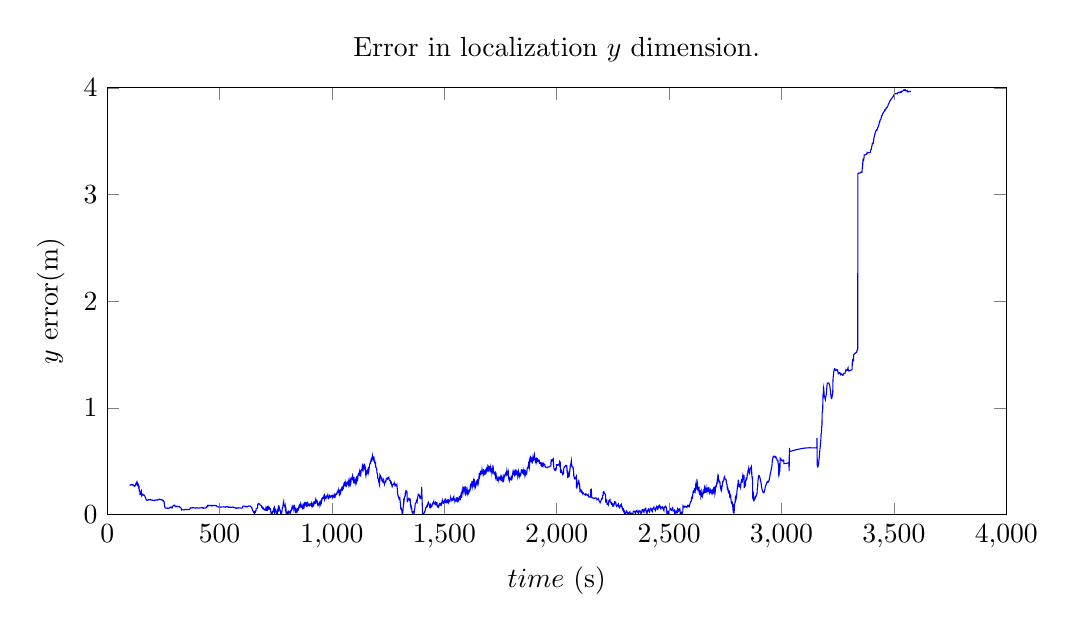
\begin{tikzpicture}

\begin{axis}[
title={Error in localization $y$ dimension.},
xlabel={$time$ (s)},
ylabel={$y$ error(m)},
xmin=0, xmax=4000,
ymin=0, ymax=4,
axis on top,
width=13cm,
height=7cm
]
\addplot [blue]
coordinates {
(100,0.277600574510846)
(101,0.276392662729327)
(102,0.277581317557389)
(103,0.277523267396756)
(104,0.275824938608006)
(105,0.2768233507361)
(106,0.2776641400418)
(107,0.280510526808398)
(108,0.280739648793641)
(109,0.280069501353818)
(110,0.279660290244103)
(111,0.279152735204871)
(112,0.278759169443993)
(113,0.278789876618309)
(114,0.279178129467409)
(115,0.272640140394363)
(116,0.272966141357732)
(117,0.274657903113424)
(118,0.270256338223822)
(119,0.270635077746235)
(120,0.268642566556268)
(121,0.269155998605685)
(122,0.265593027017736)
(123,0.267244729724979)
(124,0.26816716400325)
(125,0.270351950701197)
(126,0.279884420286534)
(127,0.283196409920451)
(128,0.291353265075888)
(129,0.294695918992109)
(130,0.298785495242125)
(131,0.30205087590952)
(132,0.305886574051986)
(133,0.285257570870551)
(134,0.288367588249621)
(135,0.291586174158974)
(136,0.27544235475529)
(137,0.278781455865062)
(138,0.282254115200383)
(139,0.28315606080348)
(140,0.253779076843696)
(141,0.255348490994768)
(142,0.257076819186538)
(143,0.217336500686529)
(144,0.216106307912925)
(145,0.217589716197979)
(146,0.189963279857543)
(147,0.192343203907776)
(148,0.195065706214306)
(149,0.200474957765169)
(150,0.202712205553653)
(151,0.20865073864731)
(152,0.214782840643722)
(153,0.180379172855013)
(154,0.18512127935971)
(155,0.190414375059696)
(156,0.190315752429539)
(157,0.184791069990392)
(158,0.185112833180925)
(159,0.188470324148378)
(160,0.181401542124292)
(161,0.183484452171907)
(162,0.184247365394342)
(163,0.1835732845916)
(164,0.182398199721933)
(165,0.1806777541865)
(166,0.177430174673361)
(167,0.174189646237291)
(168,0.170016805772794)
(169,0.164236479022771)
(170,0.159877476373303)
(171,0.153359567298113)
(172,0.148297849610797)
(173,0.14332404166406)
(174,0.139663960183089)
(175,0.136086898473847)
(176,0.135665006764166)
(177,0.134863764716974)
(178,0.133775513493156)
(179,0.133476808395883)
(180,0.133646608649053)
(181,0.135974528252716)
(182,0.135376524006661)
(183,0.137655082588369)
(184,0.136736281745803)
(185,0.137811005833117)
(186,0.139258944457651)
(187,0.139364738349071)
(188,0.13925176838783)
(189,0.139983268264369)
(190,0.138832830449245)
(191,0.138670273252214)
(192,0.139515649981575)
(193,0.138708900457641)
(194,0.138054008582622)
(195,0.13814723842973)
(196,0.135565089089328)
(197,0.13561863353585)
(198,0.134759115252266)
(199,0.134866002972105)
(200,0.1337913943738)
(201,0.135328338777558)
(202,0.134101123523296)
(203,0.133582669954786)
(204,0.132714343955426)
(205,0.132347710961799)
(206,0.132656170725591)
(207,0.131742055084547)
(208,0.131902127127503)
(209,0.131930112273869)
(210,0.131403036360681)
(211,0.133475243754842)
(212,0.132705762419528)
(213,0.135869748316239)
(214,0.135866687078287)
(215,0.135982011587612)
(216,0.134815681724984)
(217,0.135110121349205)
(218,0.135508085296222)
(219,0.135132563452176)
(220,0.134711697146498)
(221,0.135000438307755)
(222,0.139312109023794)
(223,0.139049445928936)
(224,0.139680501725779)
(225,0.13673896413988)
(226,0.136979893642355)
(227,0.137438449450231)
(228,0.137366972923119)
(229,0.141929655249442)
(230,0.142241439377417)
(231,0.142048755118304)
(232,0.143022320643334)
(233,0.14294171774949)
(234,0.139405208376899)
(235,0.139515723347701)
(236,0.139523824427232)
(237,0.141436895965047)
(238,0.141401936712811)
(239,0.141265512210196)
(240,0.138962952466412)
(241,0.138645957266922)
(242,0.135574623537248)
(243,0.13620882154385)
(244,0.138118888922635)
(245,0.136930025207686)
(246,0.135315676878632)
(247,0.132878135228967)
(248,0.129984225230737)
(249,0.128959060600843)
(250,0.129917790620969)
(251,0.120599949677137)
(252,0.119751318837085)
(253,0.120613310890081)
(254,0.10589321729198)
(255,0.0792489091911559)
(256,0.0767788270487482)
(257,0.0653898744641048)
(258,0.0617676463105883)
(259,0.0605798252844134)
(260,0.0617938604690318)
(261,0.0600189782469225)
(262,0.0605683887174338)
(263,0.0604877551517333)
(264,0.0609458282216147)
(265,0.0609439691134557)
(266,0.0607069563632323)
(267,0.0594978754886122)
(268,0.060103399963606)
(269,0.0576786440792039)
(270,0.057376541875767)
(271,0.0562355320004806)
(272,0.0559084652795976)
(273,0.0588862907293)
(274,0.0599640738841161)
(275,0.0611630390546729)
(276,0.0606253146369391)
(277,0.0616851274270118)
(278,0.0631196996117183)
(279,0.0638977311924624)
(280,0.0689963490834784)
(281,0.0661158568309608)
(282,0.0659938384076142)
(283,0.0666455584966963)
(284,0.0665686595642931)
(285,0.0662401994297053)
(286,0.0682976268027242)
(287,0.0674115847885468)
(288,0.0613500552754838)
(289,0.0620979719573627)
(290,0.0724197251690657)
(291,0.0765134915769696)
(292,0.0781412138866231)
(293,0.0800946086552954)
(294,0.0821830635894791)
(295,0.0837705617012512)
(296,0.0858886409862492)
(297,0.0864768253247257)
(298,0.0859397875114665)
(299,0.0869569149724621)
(300,0.0873751695808145)
(301,0.087680280648446)
(302,0.0745659841533923)
(303,0.0744405772408672)
(304,0.0747247594827418)
(305,0.0747268587919203)
(306,0.0738455847378692)
(307,0.0739530361291467)
(308,0.0767673777303903)
(309,0.0759209956043376)
(310,0.0771504636663662)
(311,0.0770330733339035)
(312,0.0753872979364547)
(313,0.0757762917698916)
(314,0.0758066787275564)
(315,0.0741529269819647)
(316,0.0746786822600121)
(317,0.0747691675857691)
(318,0.0741628894235995)
(319,0.0735703229924307)
(320,0.0735900472545996)
(321,0.0732637462256838)
(322,0.0731137316806061)
(323,0.0691793202136606)
(324,0.0681320524854896)
(325,0.0658378519620326)
(326,0.0659359521673193)
(327,0.0624947536225586)
(328,0.0612199893766725)
(329,0.0579647940584751)
(330,0.0533181974792778)
(331,0.043081531164149)
(332,0.0448391238085852)
(333,0.0443009096779052)
(334,0.0443046824427258)
(335,0.043239084666463)
(336,0.043632108239108)
(337,0.0443349588033741)
(338,0.0452368860548225)
(339,0.0451242935727394)
(340,0.0441707199606793)
(341,0.0435928073633023)
(342,0.0438136898121098)
(343,0.0445293877132982)
(344,0.0454147498316297)
(345,0.0448799702174787)
(346,0.0453842721233038)
(347,0.047744385709426)
(348,0.0465632450589384)
(349,0.0466879368261641)
(350,0.0463169289756813)
(351,0.047503606544347)
(352,0.046443768629433)
(353,0.0465645948371756)
(354,0.0464990825198344)
(355,0.0459666316944118)
(356,0.0466430948788319)
(357,0.0471100831695774)
(358,0.0474780580932816)
(359,0.0466751464339326)
(360,0.0477075667256086)
(361,0.0479763923796472)
(362,0.0484819622565564)
(363,0.0488406636139795)
(364,0.0485640852862237)
(365,0.047281198962291)
(366,0.0489789777451688)
(367,0.0503550170752742)
(368,0.0515716583374175)
(369,0.057207562422668)
(370,0.0613676319393641)
(371,0.0623322423286741)
(372,0.0640098858539764)
(373,0.0629836239588264)
(374,0.0627129704484557)
(375,0.0621255962203278)
(376,0.0612882206719787)
(377,0.0615605564381116)
(378,0.0617486197032129)
(379,0.0631906117255649)
(380,0.0630734367316026)
(381,0.0634541017162076)
(382,0.0629838998389056)
(383,0.062999386454293)
(384,0.0632566017634577)
(385,0.063018655907221)
(386,0.0629585273504016)
(387,0.0628177310436104)
(388,0.0625282388244579)
(389,0.062091794478548)
(390,0.0619763213258149)
(391,0.059399203466588)
(392,0.0599460333688264)
(393,0.0608207947091146)
(394,0.0611808537138216)
(395,0.0610928179830812)
(396,0.0609699406018236)
(397,0.0629576852153653)
(398,0.0629701676799419)
(399,0.0632022199389617)
(400,0.0637627763470325)
(401,0.0620894697490022)
(402,0.0614594467103928)
(403,0.0616938221353314)
(404,0.0609617990673734)
(405,0.0602258179710713)
(406,0.0606489302171815)
(407,0.0606057180909594)
(408,0.0604101517916527)
(409,0.0609418553667753)
(410,0.0607215470731242)
(411,0.0614680190302819)
(412,0.0614927573490269)
(413,0.061842388709159)
(414,0.0617870972561048)
(415,0.0618088854635594)
(416,0.062263649299712)
(417,0.0625402332289156)
(418,0.0635291592448883)
(419,0.0630701933237954)
(420,0.0632595345939713)
(421,0.0627377746423043)
(422,0.0630380471542153)
(423,0.0628915844731481)
(424,0.0624803549046233)
(425,0.0629638778574177)
(426,0.0592730372422601)
(427,0.058092984773729)
(428,0.0578431228859957)
(429,0.0613624043651115)
(430,0.0620069011678903)
(431,0.0605535897639031)
(432,0.0606795942941081)
(433,0.0603221461702743)
(434,0.0598759242475233)
(435,0.0598475472894511)
(436,0.0594694318107578)
(437,0.0599462322365905)
(438,0.0602920953284793)
(439,0.0613819515237979)
(440,0.0655330681802289)
(441,0.0692490444742972)
(442,0.066955673393184)
(443,0.0691359224714221)
(444,0.0725829405336351)
(445,0.0720726153755873)
(446,0.0822130858084433)
(447,0.0862893186458407)
(448,0.0866884243931381)
(449,0.086122870839862)
(450,0.0827582254671104)
(451,0.0846436938391935)
(452,0.0849226391787927)
(453,0.0853234049156435)
(454,0.0862750752513448)
(455,0.0861132840866903)
(456,0.0867114767593349)
(457,0.0842738872612281)
(458,0.0836238831331602)
(459,0.0837153842646794)
(460,0.0844208222936649)
(461,0.0809992963265125)
(462,0.0806907706609237)
(463,0.0807663560699465)
(464,0.0804942601521517)
(465,0.0857093443397927)
(466,0.0852170338827389)
(467,0.085035987826807)
(468,0.0823726590087608)
(469,0.0822097746336135)
(470,0.0818795105945296)
(471,0.084863085348629)
(472,0.0855686552333665)
(473,0.085169108775891)
(474,0.0852157494809997)
(475,0.0836300661985159)
(476,0.0837936227814575)
(477,0.0837448590536436)
(478,0.0845804772538954)
(479,0.0844070055970847)
(480,0.0843475399347358)
(481,0.0839113566381853)
(482,0.0837222260379784)
(483,0.0837124105944489)
(484,0.083706277040569)
(485,0.0844795783840739)
(486,0.0837165843058076)
(487,0.0790863096397416)
(488,0.077384861076689)
(489,0.0727253787947002)
(490,0.0719226057641813)
(491,0.0719605423604142)
(492,0.0721224153170921)
(493,0.0723472864998409)
(494,0.072523395831769)
(495,0.0716348687101291)
(496,0.0703370847097005)
(497,0.0697465344681545)
(498,0.0673788030752416)
(499,0.0673874978456546)
(500,0.0682574081962426)
(501,0.068379258482643)
(502,0.068840376398716)
(503,0.070837506816436)
(504,0.0715071618058989)
(505,0.0709079425391956)
(506,0.0708292002287636)
(507,0.0715505821413962)
(508,0.0702609979167574)
(509,0.0709836570242461)
(510,0.069861994849894)
(511,0.0710206523795214)
(512,0.070837029146301)
(513,0.0713676238300724)
(514,0.0717830897695788)
(515,0.071732369534097)
(516,0.0723380774912368)
(517,0.0721794450731075)
(518,0.0723283312772525)
(519,0.0712853546745627)
(520,0.0715635958164662)
(521,0.0711544849519745)
(522,0.0712049415607177)
(523,0.0688217362112566)
(524,0.0688705690915077)
(525,0.0678515521565668)
(526,0.0699268454559592)
(527,0.0703145817730984)
(528,0.0704360478475046)
(529,0.0735283233071402)
(530,0.0733419392960735)
(531,0.0735452389104116)
(532,0.0735635263379359)
(533,0.0739753274311794)
(534,0.0741778016687009)
(535,0.0741793247123876)
(536,0.0714334020873091)
(537,0.0707904627420843)
(538,0.0703323242019476)
(539,0.0681184990388561)
(540,0.0664778583568326)
(541,0.0658682838148192)
(542,0.0697866465735597)
(543,0.0680800988940247)
(544,0.0685433248479144)
(545,0.068782878712879)
(546,0.0685127302220971)
(547,0.0688688511441349)
(548,0.069075458497212)
(549,0.0670172161279972)
(550,0.0668660135051198)
(551,0.0670512547961368)
(552,0.0670948312754343)
(553,0.0687659236293081)
(554,0.068262766327654)
(555,0.0678451491877143)
(556,0.0678469819863317)
(557,0.0701542070239323)
(558,0.0698709529179053)
(559,0.0698045587278258)
(560,0.0700582505953462)
(561,0.0697544645276857)
(562,0.0695943320809174)
(563,0.0651985845610663)
(564,0.065076395686829)
(565,0.0645277004078761)
(566,0.0657721714141961)
(567,0.0639953578240395)
(568,0.062179345807627)
(569,0.062490858663574)
(570,0.0626370599855868)
(571,0.0628185332823303)
(572,0.0592543562896735)
(573,0.058819829295421)
(574,0.0586811656094763)
(575,0.0584052610285881)
(576,0.062187396411336)
(577,0.0621521261094462)
(578,0.0624498797759188)
(579,0.0606917791031942)
(580,0.0609176902622122)
(581,0.0602692348484406)
(582,0.0599910442534144)
(583,0.0616318331256052)
(584,0.0611726464642803)
(585,0.061153999768119)
(586,0.0629817983633632)
(587,0.0618241319996922)
(588,0.0617650387445088)
(589,0.062389276963827)
(590,0.0617395482450003)
(591,0.0618486443864015)
(592,0.0625138288192297)
(593,0.0605914087121913)
(594,0.0605109940200266)
(595,0.0596972796834812)
(596,0.0597968296309328)
(597,0.0597904460542829)
(598,0.0599489440586183)
(599,0.0602110597575911)
(600,0.0599317453696258)
(601,0.0598281849577442)
(602,0.0626604719404771)
(603,0.0760713375898656)
(604,0.0777232950395232)
(605,0.0781401786489266)
(606,0.0783787388563977)
(607,0.0789237844363688)
(608,0.0794026415138824)
(609,0.0788548832528781)
(610,0.0789426421435144)
(611,0.0787495063533155)
(612,0.0785099692466344)
(613,0.0748020931035076)
(614,0.0762468612963283)
(615,0.0734736495082795)
(616,0.0756808440471168)
(617,0.0742291721398014)
(618,0.0740003452614482)
(619,0.0748740356868534)
(620,0.0749355201944146)
(621,0.0752585312525911)
(622,0.0721987252152041)
(623,0.0737748331600541)
(624,0.0734929893340568)
(625,0.0726581298950131)
(626,0.0750746694681976)
(627,0.0766803226225812)
(628,0.0783523909565198)
(629,0.0790270820070669)
(630,0.0789919169922522)
(631,0.0808621279553328)
(632,0.0806728350863439)
(633,0.0799045423182303)
(634,0.0793496587944098)
(635,0.0807218982836275)
(636,0.0798885017470603)
(637,0.0783705999749107)
(638,0.0764417763101468)
(639,0.0749306065437407)
(640,0.0715927653245418)
(641,0.0699169954727847)
(642,0.0669136801500687)
(643,0.0612377651067333)
(644,0.0582239696017881)
(645,0.0526525555278012)
(646,0.0434662723380139)
(647,0.0382519184583314)
(648,0.03457015509577)
(649,0.0308465489150014)
(650,0.0280098019961792)
(651,0.0219514958193949)
(652,0.0192657087915125)
(653,0.0155987112468283)
(654,0.0129223520668331)
(655,0.00996916156934669)
(656,0.0233321592973827)
(657,0.0205496882558416)
(658,0.0183110466095733)
(659,0.0179992744836275)
(660,0.0330139134424563)
(661,0.0328981525973919)
(662,0.0353996172330064)
(663,0.0546935919961338)
(664,0.0573747347408378)
(665,0.0582686128256364)
(666,0.0584562591437878)
(667,0.058136227788625)
(668,0.0595003420565763)
(669,0.0610224640678725)
(670,0.097012184809985)
(671,0.0986393007536659)
(672,0.0990357719864714)
(673,0.100171545301337)
(674,0.102516965244288)
(675,0.100784572402343)
(676,0.101071594243629)
(677,0.0970947795438604)
(678,0.0971950526913994)
(679,0.0968078555438647)
(680,0.0895628875797514)
(681,0.0893014753296142)
(682,0.0880857938099671)
(683,0.0865062606708067)
(684,0.0861580319301676)
(685,0.084180313332181)
(686,0.0821158479045554)
(687,0.0714959689122199)
(688,0.067845084775223)
(689,0.0712812321301604)
(690,0.0710344207521936)
(691,0.0645795776754934)
(692,0.0563190069035171)
(693,0.0540597314575915)
(694,0.0567057274934752)
(695,0.0587166648524207)
(696,0.0516416449674471)
(697,0.0511674110404163)
(698,0.0457995405069549)
(699,0.0432447869262744)
(700,0.0427842225835602)
(701,0.0486206350662286)
(702,0.048717191151177)
(703,0.0451811796921304)
(704,0.0503407234814279)
(705,0.0418757015030922)
(706,0.0417862167957685)
(707,0.0628832560211676)
(708,0.0583600817559531)
(709,0.0499249076392054)
(710,0.0566479928126369)
(711,0.0411785195972705)
(712,0.0386788323577743)
(713,0.0424543621367164)
(714,0.0725727371303564)
(715,0.0759658772490917)
(716,0.0664157651595048)
(717,0.0590635427209145)
(718,0.0546879195098948)
(719,0.0593895078674529)
(720,0.0702279664106737)
(721,0.0698505633068907)
(722,0.0577976341918909)
(723,0.0492953785056125)
(724,0.0484581350780653)
(725,0.0518049338100584)
(726,0.0526097613994336)
(727,0.0416397917822482)
(728,0.0214734560876693)
(729,0.0144216734549638)
(730,0.00508929884059128)
(731,0.0178199313093601)
(732,0.0144583251266628)
(733,0.00250816047209357)
(734,0.00800986536949821)
(735,0.017691507666048)
(736,0.0270654297514343)
(737,0.0252514349433537)
(738,0.024444831452501)
(739,0.0263526402862264)
(740,0.0370593630709366)
(741,0.0567372756009874)
(742,0.0577201949022359)
(743,0.0651701787149923)
(744,0.0692012605139505)
(745,0.0265841688091726)
(746,0.0390719874092311)
(747,0.0501373958005611)
(748,0.0506741504644777)
(749,0.0495926535082605)
(750,0.0427133966187321)
(751,0.0341327402298917)
(752,0.0125337511324264)
(753,0.00892126392581361)
(754,0.0119782686412435)
(755,0.00845629884375132)
(756,0.0131827976872509)
(757,0.0235151978150445)
(758,0.0181907402744539)
(759,0.043486430856865)
(760,0.0400869453027166)
(761,0.0377611110570073)
(762,0.0764813752044748)
(763,0.0817760924362241)
(764,0.0811656135001977)
(765,0.0723748849373615)
(766,0.0471897065246734)
(767,0.0427018175418703)
(768,0.0411452569950645)
(769,0.0346190754319684)
(770,0.0383823450677578)
(771,0.0320067653757681)
(772,0.00382752173300771)
(773,0.00443035618026322)
(774,0.00356010888004255)
(775,0.00544426141029319)
(776,0.0139421030759554)
(777,0.0232369780349315)
(778,0.0372389191959934)
(779,0.060348659083878)
(780,0.058779521050587)
(781,0.0648696398663335)
(782,0.0788179029773532)
(783,0.0983030494930599)
(784,0.112248165813652)
(785,0.121187481980674)
(786,0.0916629976782279)
(787,0.089468581625213)
(788,0.083056593345511)
(789,0.0812177059517927)
(790,0.0755614682946102)
(791,0.0799374477685824)
(792,0.0861156349191226)
(793,0.0374384175876412)
(794,0.0357667435276348)
(795,0.026255205979179)
(796,0.0382246050586188)
(797,0.0186490173830345)
(798,0.0198846251828591)
(799,0.0200354798094251)
(800,0.0101942276212523)
(801,0.0134277763295851)
(802,0.0121305464158401)
(803,0.00911144159867261)
(804,0.0269370875816493)
(805,0.0293118324432751)
(806,0.0156819566023998)
(807,0.0202852434136696)
(808,0.0240386093768987)
(809,0.0253972831153457)
(810,0.0242869827601413)
(811,0.0248963807071712)
(812,0.025577734576586)
(813,0.00475948604156651)
(814,0.00740907334935992)
(815,0.0178395387838002)
(816,0.0345237559710685)
(817,0.0382034035974352)
(818,0.0373057182654999)
(819,0.0359413714495016)
(820,0.0462670862011625)
(821,0.0585005917711698)
(822,0.0693016618503592)
(823,0.0751017806458343)
(824,0.0631355086715191)
(825,0.0609136384173783)
(826,0.0565760202912413)
(827,0.0588829770432455)
(828,0.0628577804903894)
(829,0.0737551118230919)
(830,0.0785025083847319)
(831,0.04602203180381)
(832,0.0547732371954477)
(833,0.0629120916458263)
(834,0.0720681555121043)
(835,0.065011145947893)
(836,0.0635962999390962)
(837,0.0596849928081014)
(838,0.0201894119413337)
(839,0.0218875356673651)
(840,0.027251694770527)
(841,0.0484294241808048)
(842,0.0513583578321959)
(843,0.0518505127410709)
(844,0.0219500010897185)
(845,0.0242793467575813)
(846,0.0380396998989241)
(847,0.048700634330257)
(848,0.0449124806323784)
(849,0.0465800335771833)
(850,0.043645996402164)
(851,0.0521876118402664)
(852,0.0634090590003873)
(853,0.0768333397625542)
(854,0.082218691869429)
(855,0.0763869726179562)
(856,0.0720461395065186)
(857,0.0852043547075829)
(858,0.0911005347132674)
(859,0.0984880477410268)
(860,0.0790746319192781)
(861,0.0786474033140934)
(862,0.0753869183712728)
(863,0.0687931570839782)
(864,0.0719948638354699)
(865,0.0829722097355048)
(866,0.0893740392770304)
(867,0.0691676656950611)
(868,0.0665737017546038)
(869,0.0599652429207995)
(870,0.0654914980437042)
(871,0.0714327913840731)
(872,0.0801154275879519)
(873,0.0604245022919563)
(874,0.0633030757070498)
(875,0.0596498435293551)
(876,0.0604640104047105)
(877,0.0879020393274352)
(878,0.10332271651159)
(879,0.108436506760266)
(880,0.086480752990421)
(881,0.0871755121952273)
(882,0.0944000346281744)
(883,0.098175337142635)
(884,0.11078398460608)
(885,0.111763044333633)
(886,0.110345016466523)
(887,0.0780737929123094)
(888,0.0792843694692262)
(889,0.0829649339706666)
(890,0.0989121415183343)
(891,0.106141949195168)
(892,0.110963807387356)
(893,0.105307595119561)
(894,0.0850006717541643)
(895,0.0877735853119654)
(896,0.0942831685941812)
(897,0.0951304107936544)
(898,0.0924146020822283)
(899,0.0880178775768323)
(900,0.0842610679062719)
(901,0.089212947198039)
(902,0.0916290742929537)
(903,0.100590231969653)
(904,0.0994015414812051)
(905,0.0925603995246833)
(906,0.0951449775908286)
(907,0.0894559254359528)
(908,0.0997638156806024)
(909,0.105935421067136)
(910,0.0858870401248315)
(911,0.0834342545473308)
(912,0.0726284058777154)
(913,0.0773593628705616)
(914,0.0848245874101163)
(915,0.0942315481000477)
(916,0.102286636714295)
(917,0.0879119798482226)
(918,0.0838553903416481)
(919,0.0917186521205049)
(920,0.0994888742385265)
(921,0.109253953993326)
(922,0.116034902906155)
(923,0.119061515958473)
(924,0.104508856900068)
(925,0.103829027058819)
(926,0.110367001508669)
(927,0.133243624352034)
(928,0.141831384806408)
(929,0.12972325763868)
(930,0.117170296128763)
(931,0.123952946592122)
(932,0.1265668426708)
(933,0.130532088033628)
(934,0.125819170025617)
(935,0.124031311866469)
(936,0.118378954867011)
(937,0.0900372957054625)
(938,0.0936650070079774)
(939,0.0986583008296265)
(940,0.0950431124565601)
(941,0.0990446897567874)
(942,0.0998790559374894)
(943,0.0884561769119703)
(944,0.102384501216326)
(945,0.111681007845732)
(946,0.116781097781423)
(947,0.101595270328338)
(948,0.099677493770943)
(949,0.093991239568159)
(950,0.108649179990599)
(951,0.113688104947263)
(952,0.126922572633827)
(953,0.133944234592632)
(954,0.122429605164875)
(955,0.13562776801041)
(956,0.145483339397673)
(957,0.153321649725279)
(958,0.159406963598518)
(959,0.158994239488372)
(960,0.150856655777906)
(961,0.151282504916438)
(962,0.15233552726558)
(963,0.159697865783711)
(964,0.175201536410161)
(965,0.181656133462365)
(966,0.184192516047014)
(967,0.144786218710574)
(968,0.152401392747497)
(969,0.163897125038996)
(970,0.151983996332856)
(971,0.151706489884847)
(972,0.150261004447838)
(973,0.149167975401352)
(974,0.152402724634209)
(975,0.158747574240784)
(976,0.175043503737268)
(977,0.174844836423016)
(978,0.172883002178855)
(979,0.171895285861174)
(980,0.173672619259898)
(981,0.180385499717905)
(982,0.155981470459878)
(983,0.155652445103049)
(984,0.154396873254841)
(985,0.150749812110816)
(986,0.155872269595371)
(987,0.163937835913158)
(988,0.173190666478741)
(989,0.166276613920028)
(990,0.164894025136309)
(991,0.171516629664157)
(992,0.165744636798603)
(993,0.172734304529495)
(994,0.17483867402423)
(995,0.174479237475636)
(996,0.166887722755413)
(997,0.16970375789457)
(998,0.17286510644819)
(999,0.172738126159826)
(1000,0.178512637764029)
(1001,0.177007992332131)
(1002,0.161402132625101)
(1003,0.168278805751594)
(1004,0.173761642246404)
(1005,0.179843412509537)
(1006,0.171570072439389)
(1007,0.172716603776313)
(1008,0.162962296496325)
(1009,0.160930789179827)
(1010,0.15980246315206)
(1011,0.17292278531673)
(1012,0.182350804399794)
(1013,0.172429193836157)
(1014,0.167740587725111)
(1015,0.178751798936521)
(1016,0.17754423720978)
(1017,0.19023873553051)
(1018,0.192783452851381)
(1019,0.194771420414486)
(1020,0.189733329481623)
(1021,0.188935674582566)
(1022,0.193259761151971)
(1023,0.20459093005811)
(1024,0.215679990575795)
(1025,0.217024278583618)
(1026,0.21428110218455)
(1027,0.222349725721648)
(1028,0.231253786021779)
(1029,0.216057010729818)
(1030,0.219992818176137)
(1031,0.222219832673498)
(1032,0.197695464979129)
(1033,0.185315264663917)
(1034,0.190648776924048)
(1035,0.20389934955092)
(1036,0.221512260083855)
(1037,0.231078723006799)
(1038,0.230368002112727)
(1039,0.209859894766449)
(1040,0.218786672374223)
(1041,0.23191977540804)
(1042,0.242260930228908)
(1043,0.23382800779631)
(1044,0.233685437345066)
(1045,0.228492434373146)
(1046,0.227486983039491)
(1047,0.234948766056629)
(1048,0.257587304836559)
(1049,0.262823678851668)
(1050,0.254942517864627)
(1051,0.251242826743661)
(1052,0.265559877283671)
(1053,0.276475272120826)
(1054,0.297023475467504)
(1055,0.30114798615767)
(1056,0.303563230316734)
(1057,0.301950477165345)
(1058,0.293623151389967)
(1059,0.264748595764084)
(1060,0.281733528916986)
(1061,0.294563653350138)
(1062,0.269523391901965)
(1063,0.263853353413879)
(1064,0.265320626984961)
(1065,0.281429894724464)
(1066,0.285033408089252)
(1067,0.296435634586763)
(1068,0.300468659482593)
(1069,0.302252004649483)
(1070,0.289654252258181)
(1071,0.285476474781735)
(1072,0.301489596018588)
(1073,0.295847940920804)
(1074,0.30621687785805)
(1075,0.316964030771836)
(1076,0.268198000759483)
(1077,0.272989126125269)
(1078,0.284455838471555)
(1079,0.302168313884247)
(1080,0.316306039297699)
(1081,0.323937185691435)
(1082,0.328553134801365)
(1083,0.288376579638625)
(1084,0.296330132928383)
(1085,0.317325510181297)
(1086,0.337023361020818)
(1087,0.338969262950739)
(1088,0.340876772813566)
(1089,0.34763843670569)
(1090,0.338780086226574)
(1091,0.352008665373089)
(1092,0.363357128452979)
(1093,0.351037955038709)
(1094,0.347917117898906)
(1095,0.338225703452807)
(1096,0.320109216524084)
(1097,0.33193102701559)
(1098,0.350834581298401)
(1099,0.313651210449987)
(1100,0.317924064614465)
(1101,0.305678976114433)
(1102,0.309448073677722)
(1103,0.298363557702805)
(1104,0.317993707019129)
(1105,0.324556827437129)
(1106,0.300975167033276)
(1107,0.303917819534366)
(1108,0.297898004322177)
(1109,0.327674064190918)
(1110,0.346006507909493)
(1111,0.356815950004898)
(1112,0.356972995896409)
(1113,0.319491918057405)
(1114,0.32356110132448)
(1115,0.342680600385522)
(1116,0.366961194129316)
(1117,0.377986572238521)
(1118,0.381562485956991)
(1119,0.384629604395092)
(1120,0.380232402505836)
(1121,0.387563161168222)
(1122,0.399087662723586)
(1123,0.379746674700671)
(1124,0.384836927267546)
(1125,0.395091060305159)
(1126,0.384121551254971)
(1127,0.356684651125257)
(1128,0.374569616874611)
(1129,0.391282529006673)
(1130,0.413500146000234)
(1131,0.415225977351634)
(1132,0.420376902902286)
(1133,0.419891312344407)
(1134,0.432228804589577)
(1135,0.455910967645136)
(1136,0.461638384067693)
(1137,0.414651692559562)
(1138,0.41015876336552)
(1139,0.422329207596083)
(1140,0.427985380213272)
(1141,0.445675261517136)
(1142,0.457912837397702)
(1143,0.464327075578384)
(1144,0.468728980301023)
(1145,0.46424069602523)
(1146,0.462294429335898)
(1147,0.416428121897012)
(1148,0.43698398721133)
(1149,0.439335007828979)
(1150,0.377062307476283)
(1151,0.364836132828811)
(1152,0.379255206824851)
(1153,0.377850167452654)
(1154,0.393413255190523)
(1155,0.406481069384671)
(1156,0.40966647958398)
(1157,0.389899905535798)
(1158,0.384876716041387)
(1159,0.386396461090294)
(1160,0.411013990064533)
(1161,0.426561416861492)
(1162,0.436993978120585)
(1163,0.435339412592709)
(1164,0.408694247895529)
(1165,0.424049404626751)
(1166,0.44422759242424)
(1167,0.454489635110041)
(1168,0.471611962192585)
(1169,0.475771925943014)
(1170,0.483846224335194)
(1171,0.482010541830066)
(1172,0.489315207286471)
(1173,0.505726478411449)
(1174,0.51120807903426)
(1175,0.52605053771718)
(1176,0.524866241558579)
(1177,0.496323679177807)
(1178,0.514778251579636)
(1179,0.536444006412349)
(1180,0.551941862841552)
(1181,0.538947421491504)
(1182,0.527549211866684)
(1183,0.525545767172456)
(1184,0.521379505326253)
(1185,0.515007716853456)
(1186,0.525097734086185)
(1187,0.54358411231009)
(1188,0.510402508725286)
(1189,0.492806510973159)
(1190,0.488245403331616)
(1191,0.494218951207136)
(1192,0.483064050544373)
(1193,0.487091818834371)
(1194,0.486843518557483)
(1195,0.44361477953945)
(1196,0.44110257847515)
(1197,0.437568079895992)
(1198,0.434890295958574)
(1199,0.427217577584842)
(1200,0.397475343955109)
(1201,0.386588544776346)
(1202,0.3799113581605)
(1203,0.370922610523522)
(1204,0.3383712060211)
(1205,0.335760130730283)
(1206,0.335190587063642)
(1207,0.318742954435985)
(1208,0.307211777327617)
(1209,0.303144113143972)
(1210,0.296619917615548)
(1211,0.279713092768523)
(1212,0.272741534478909)
(1213,0.373402914852759)
(1214,0.369295828489306)
(1215,0.368034858433637)
(1216,0.35728253285589)
(1217,0.350125871991034)
(1218,0.35338589778685)
(1219,0.348152927311616)
(1220,0.342004631196952)
(1221,0.325054457420161)
(1222,0.319292988651391)
(1223,0.316332110158376)
(1224,0.307809498757884)
(1225,0.307021435945111)
(1226,0.306617363108003)
(1227,0.304664639096193)
(1228,0.330559820904025)
(1229,0.324809570675574)
(1230,0.324358951244551)
(1231,0.297421488066462)
(1232,0.295734314973304)
(1233,0.293644846486987)
(1234,0.283984696048482)
(1235,0.29365115115833)
(1236,0.301155040267481)
(1237,0.302708035877841)
(1238,0.310158733947255)
(1239,0.309396960984086)
(1240,0.308347167537285)
(1241,0.32773402849913)
(1242,0.336525480523237)
(1243,0.33798743920304)
(1244,0.338028166026933)
(1245,0.34099511300448)
(1246,0.337094687924409)
(1247,0.333033259068962)
(1248,0.336660403135252)
(1249,0.341056605363388)
(1250,0.33998266517785)
(1251,0.347920103370892)
(1252,0.347695109916751)
(1253,0.349832656929177)
(1254,0.331445141383123)
(1255,0.325187271392221)
(1256,0.322048831665641)
(1257,0.321825420576506)
(1258,0.318885980409998)
(1259,0.315370992283827)
(1260,0.316756583192934)
(1261,0.29636121090606)
(1262,0.29711352207952)
(1263,0.293501907373162)
(1264,0.297240440109879)
(1265,0.281836818348249)
(1266,0.276204162676645)
(1267,0.269599848836126)
(1268,0.26259639864128)
(1269,0.269277255375048)
(1270,0.271792100543698)
(1271,0.282395654230116)
(1272,0.282311677561773)
(1273,0.283608726586009)
(1274,0.285311091166627)
(1275,0.283627227832503)
(1276,0.283370705391948)
(1277,0.29430828285399)
(1278,0.284223041444449)
(1279,0.27999297973381)
(1280,0.282620736182223)
(1281,0.271141756448172)
(1282,0.273987657052382)
(1283,0.275957500005573)
(1284,0.281462509275812)
(1285,0.281816308068257)
(1286,0.270675781063476)
(1287,0.267706837387909)
(1288,0.268861498396227)
(1289,0.274336698062469)
(1290,0.252164362123489)
(1291,0.235493640628293)
(1292,0.198931143018499)
(1293,0.186497418523705)
(1294,0.176069273162567)
(1295,0.169321994033727)
(1296,0.164140374942354)
(1297,0.160982351764841)
(1298,0.148534008576155)
(1299,0.14331322380942)
(1300,0.141243430545316)
(1301,0.141969468314902)
(1302,0.149432657880717)
(1303,0.131359727506627)
(1304,0.11364308688537)
(1305,0.0885007037929655)
(1306,0.0545280716823706)
(1307,0.0507418494919518)
(1308,0.0527030507925785)
(1309,0.056191495744131)
(1310,0.0502081406793129)
(1311,0.0334277551545183)
(1312,0.0092174927496429)
(1313,0.00206038639105999)
(1314,0.00129935775221091)
(1315,0.0172416158889575)
(1316,0.0381123636671037)
(1317,0.0700713509944402)
(1318,0.0743838440293003)
(1319,0.142634928616773)
(1320,0.145714404822676)
(1321,0.133791072728229)
(1322,0.152025359982577)
(1323,0.160820642942692)
(1324,0.165648787275334)
(1325,0.172098212568887)
(1326,0.194075437939172)
(1327,0.188983589854184)
(1328,0.204962955208694)
(1329,0.2251888906124)
(1330,0.22471350998346)
(1331,0.220512697317413)
(1332,0.216280791147285)
(1333,0.213735819990143)
(1334,0.209897681390062)
(1335,0.124826450957146)
(1336,0.122625668967764)
(1337,0.127196352923814)
(1338,0.134911104926562)
(1339,0.136361596988845)
(1340,0.138622713280898)
(1341,0.147770199618981)
(1342,0.151289487919042)
(1343,0.143625346300859)
(1344,0.139984785758328)
(1345,0.144656534395164)
(1346,0.145888534341658)
(1347,0.145839767004036)
(1348,0.145956615529008)
(1349,0.0805682357998185)
(1350,0.0789495779282507)
(1351,0.0822621143449138)
(1352,0.0544260777704924)
(1353,0.0557898934362047)
(1354,0.0652809512326176)
(1355,0.0576481617449318)
(1356,0.0298397960231307)
(1357,0.0194885052548401)
(1358,0.0198711466177905)
(1359,0.0216288012689065)
(1360,0.0105798290854333)
(1361,0.00623120487603734)
(1362,0.0144389585505873)
(1363,0.0204592434163657)
(1364,0.0280112502622802)
(1365,0.0268269409078337)
(1366,0.0219600605717667)
(1367,0.0351565791812765)
(1368,0.0519432540553211)
(1369,0.0614927656177622)
(1370,0.0972815178795372)
(1371,0.102071088364748)
(1372,0.108069987559247)
(1373,0.108648488209286)
(1374,0.112581041915276)
(1375,0.115523831007857)
(1376,0.128986403101253)
(1377,0.133525472692381)
(1378,0.129264397470737)
(1379,0.121741887378763)
(1380,0.142046117155856)
(1381,0.156884891936601)
(1382,0.166648034245218)
(1383,0.173198498481883)
(1384,0.189291276059869)
(1385,0.186894133003703)
(1386,0.180909562592077)
(1387,0.180377549303215)
(1388,0.180937661241463)
(1389,0.182261194276343)
(1390,0.179243971286606)
(1391,0.157651134951392)
(1392,0.1595064705962)
(1393,0.156564761749272)
(1394,0.17066985902843)
(1395,0.171234860266906)
(1396,0.168701419127346)
(1397,0.16722566439111)
(1398,0.14475877384686)
(1399,0.257971624528693)
(1400,0.195937213212118)
(1401,0.137703626925852)
(1402,0.0734335733157703)
(1403,0.0184678444056934)
(1404,0.00140407596413072)
(1405,0.00109498824717602)
(1406,0.00150138538123712)
(1407,0.00119408699980927)
(1408,0.00284851867305136)
(1409,0.0107183966229085)
(1410,0.0129839797069842)
(1411,0.0181393193194839)
(1412,0.0226260758134955)
(1413,0.0295700562427479)
(1414,0.0347892914496128)
(1415,0.0420158517440932)
(1416,0.0506600669659274)
(1417,0.0595722066992539)
(1418,0.0667349818945502)
(1419,0.0667530508323142)
(1420,0.0654807241196902)
(1421,0.0676353950170727)
(1422,0.0817648900276804)
(1423,0.0876857826021507)
(1424,0.0886576430357933)
(1425,0.0840413265335165)
(1426,0.0949351493987056)
(1427,0.105235300859006)
(1428,0.111740649994797)
(1429,0.115832393906687)
(1430,0.111864946265854)
(1431,0.101702374668174)
(1432,0.0982207253912417)
(1433,0.096818965821083)
(1434,0.0825706758379758)
(1435,0.0885885817016336)
(1436,0.0883235329106156)
(1437,0.0723702418232504)
(1438,0.0808744842178206)
(1439,0.0894550280338451)
(1440,0.082199276136407)
(1441,0.0884706199606613)
(1442,0.0874526197274941)
(1443,0.0828755096241673)
(1444,0.0757874245426691)
(1445,0.081070444165577)
(1446,0.0883863099339139)
(1447,0.100165120477271)
(1448,0.0966699382700698)
(1449,0.0957263938886248)
(1450,0.0995099115945495)
(1451,0.110116808551529)
(1452,0.113913178848748)
(1453,0.12117673597366)
(1454,0.108364553487972)
(1455,0.106307293868774)
(1456,0.10511170753245)
(1457,0.106103957913924)
(1458,0.100349352355718)
(1459,0.105178609738894)
(1460,0.111105998358826)
(1461,0.0990459893410636)
(1462,0.0905266665056994)
(1463,0.0912298478986635)
(1464,0.099212176333983)
(1465,0.110573830373732)
(1466,0.112811716162504)
(1467,0.113226625731711)
(1468,0.0804786968122548)
(1469,0.0765907685023157)
(1470,0.0757182802241259)
(1471,0.0712854120152224)
(1472,0.0756284224244836)
(1473,0.0802325294425819)
(1474,0.0755309189803188)
(1475,0.0713024950550067)
(1476,0.0840225680599376)
(1477,0.0895109472383464)
(1478,0.100176735189793)
(1479,0.104660190917915)
(1480,0.105395191199347)
(1481,0.10306112697309)
(1482,0.0884934149317833)
(1483,0.0898225532894352)
(1484,0.0914481286276969)
(1485,0.0957979935420501)
(1486,0.10030646032096)
(1487,0.0928285409380736)
(1488,0.100353413956572)
(1489,0.113285532036573)
(1490,0.122529111186875)
(1491,0.13197031906759)
(1492,0.120270839490984)
(1493,0.119562721065344)
(1494,0.110594537640576)
(1495,0.106564236639099)
(1496,0.106298945074947)
(1497,0.113746825745926)
(1498,0.119916551015945)
(1499,0.112426829613561)
(1500,0.111723790453689)
(1501,0.118469821386206)
(1502,0.128506538499837)
(1503,0.140656948898294)
(1504,0.146584224552752)
(1505,0.146721951895885)
(1506,0.11152327284771)
(1507,0.110561791697013)
(1508,0.113046410227786)
(1509,0.119987848930258)
(1510,0.12785558855401)
(1511,0.130487082607188)
(1512,0.110334793726475)
(1513,0.111141296737111)
(1514,0.124058512943598)
(1515,0.133950512013489)
(1516,0.136070252562982)
(1517,0.135994905707683)
(1518,0.136707325788421)
(1519,0.113615099527643)
(1520,0.1182888435637)
(1521,0.119145994288921)
(1522,0.124114766814322)
(1523,0.129883790881371)
(1524,0.129274613554418)
(1525,0.126323416451642)
(1526,0.139651846141063)
(1527,0.14865829764698)
(1528,0.159270535776056)
(1529,0.146235502145431)
(1530,0.145777131219596)
(1531,0.141634333674878)
(1532,0.139822579288785)
(1533,0.132772765370762)
(1534,0.136705453838992)
(1535,0.142580176801922)
(1536,0.136413469067704)
(1537,0.132535550974123)
(1538,0.131935819556174)
(1539,0.138795241680388)
(1540,0.155973388850039)
(1541,0.161991158794623)
(1542,0.166797548420301)
(1543,0.143320805491694)
(1544,0.138796446743064)
(1545,0.138270305252498)
(1546,0.140359254585854)
(1547,0.124073250758385)
(1548,0.132299787615179)
(1549,0.129680354429905)
(1550,0.127948230424644)
(1551,0.126816905128421)
(1552,0.136133107833053)
(1553,0.151346552070874)
(1554,0.147808143736675)
(1555,0.153762707229838)
(1556,0.155081395484084)
(1557,0.131684359001172)
(1558,0.12457240188491)
(1559,0.128990224394783)
(1560,0.14224178548986)
(1561,0.150418499996342)
(1562,0.148567754726222)
(1563,0.135910547968497)
(1564,0.129631656565478)
(1565,0.140925023470404)
(1566,0.15498482870514)
(1567,0.174951737760953)
(1568,0.149794980386427)
(1569,0.149755137510147)
(1570,0.150897634009849)
(1571,0.146657501937172)
(1572,0.158148173909815)
(1573,0.178963097383183)
(1574,0.187423014928742)
(1575,0.169541388126933)
(1576,0.162752453092108)
(1577,0.16185958464958)
(1578,0.187531375026546)
(1579,0.207388578811447)
(1580,0.228094558400604)
(1581,0.210109306325903)
(1582,0.218760119708943)
(1583,0.217082108575404)
(1584,0.227018111008356)
(1585,0.232175716085619)
(1586,0.249541494260218)
(1587,0.246067834699513)
(1588,0.211132147219426)
(1589,0.222218177226433)
(1590,0.234806536017408)
(1591,0.251822686925161)
(1592,0.259246902445456)
(1593,0.258221470057327)
(1594,0.25622325575256)
(1595,0.196870645830647)
(1596,0.202817209899732)
(1597,0.216313183099807)
(1598,0.226131373956621)
(1599,0.208495432243909)
(1600,0.198333993319348)
(1601,0.199942147577564)
(1602,0.192439753227933)
(1603,0.209840675062926)
(1604,0.223736222791347)
(1605,0.198668180525556)
(1606,0.197978923726601)
(1607,0.195230932821815)
(1608,0.204021080654056)
(1609,0.212607222623521)
(1610,0.222711054997874)
(1611,0.219678074247548)
(1612,0.215179321615902)
(1613,0.216629907496974)
(1614,0.230183206678482)
(1615,0.24860679578644)
(1616,0.27477830805399)
(1617,0.284273263046275)
(1618,0.284348560242354)
(1619,0.260847535280209)
(1620,0.267568888695906)
(1621,0.278071024535592)
(1622,0.295158017848917)
(1623,0.29071273677948)
(1624,0.303471196320719)
(1625,0.300345297012518)
(1626,0.271189079633173)
(1627,0.285860052518852)
(1628,0.306042868998526)
(1629,0.314270832425628)
(1630,0.276783024472297)
(1631,0.274497966740297)
(1632,0.286416305634278)
(1633,0.25526157224521)
(1634,0.27136197874333)
(1635,0.294394107479817)
(1636,0.278706185985925)
(1637,0.248515211034323)
(1638,0.253258047023015)
(1639,0.260017221278988)
(1640,0.268541590977303)
(1641,0.285044185370201)
(1642,0.307274053494434)
(1643,0.310247217491838)
(1644,0.290997437045163)
(1645,0.285698662251015)
(1646,0.299900287433578)
(1647,0.315082954153815)
(1648,0.326022658496156)
(1649,0.327811558327614)
(1650,0.32000608072717)
(1651,0.2946687719401)
(1652,0.305932362093059)
(1653,0.323667357832652)
(1654,0.343553129815118)
(1655,0.382228159075973)
(1656,0.38408674055856)
(1657,0.385214836269709)
(1658,0.366738549345534)
(1659,0.377359927723238)
(1660,0.38960714204829)
(1661,0.410631297472626)
(1662,0.387512955026541)
(1663,0.387230118420185)
(1664,0.378585719931483)
(1665,0.380054910834639)
(1666,0.401737643773821)
(1667,0.41617258201179)
(1668,0.392178570887635)
(1669,0.393758120670039)
(1670,0.394272752814908)
(1671,0.398172947356574)
(1672,0.384325139482121)
(1673,0.404822591353394)
(1674,0.427809220089008)
(1675,0.382171519032501)
(1676,0.371831877007191)
(1677,0.371760718256411)
(1678,0.382530738908859)
(1679,0.38740037320267)
(1680,0.406039249584314)
(1681,0.410080751074168)
(1682,0.383485998317391)
(1683,0.383160574569689)
(1684,0.381293247273655)
(1685,0.387369905788528)
(1686,0.405380330315299)
(1687,0.421418939212152)
(1688,0.410888591572711)
(1689,0.402116788859831)
(1690,0.403499850164154)
(1691,0.414110372524956)
(1692,0.434317066341815)
(1693,0.435009759050489)
(1694,0.458955835735354)
(1695,0.455883726390588)
(1696,0.447928305110251)
(1697,0.422630685537894)
(1698,0.43083004251701)
(1699,0.43846534492076)
(1700,0.431933356262137)
(1701,0.436544426623721)
(1702,0.419443968889186)
(1703,0.408260338121069)
(1704,0.404868440786095)
(1705,0.416101890271214)
(1706,0.436858792191974)
(1707,0.420693844329082)
(1708,0.423808274885472)
(1709,0.425043649068368)
(1710,0.41984719828018)
(1711,0.399213522946745)
(1712,0.419118879385471)
(1713,0.432046472511529)
(1714,0.408759635341112)
(1715,0.399982361853466)
(1716,0.406751379346085)
(1717,0.412465471222227)
(1718,0.425591240483385)
(1719,0.404828906735498)
(1720,0.403194728543818)
(1721,0.380781346439683)
(1722,0.380009495997702)
(1723,0.381966682911893)
(1724,0.376972249009606)
(1725,0.389802310600772)
(1726,0.390268712353265)
(1727,0.393363481127512)
(1728,0.362942600965131)
(1729,0.376597627348198)
(1730,0.391900256033963)
(1731,0.357330341774652)
(1732,0.362993411097047)
(1733,0.360514176072063)
(1734,0.324079558781467)
(1735,0.322133270891136)
(1736,0.32988383873705)
(1737,0.34217401710189)
(1738,0.3409496040092)
(1739,0.334091738020115)
(1740,0.322377153020572)
(1741,0.33304863284308)
(1742,0.344006952278711)
(1743,0.350028560622136)
(1744,0.345979057724124)
(1745,0.345860838229634)
(1746,0.34143309681433)
(1747,0.334010476555324)
(1748,0.340285354516051)
(1749,0.349930111989684)
(1750,0.336429508909136)
(1751,0.337744680510417)
(1752,0.32699464479248)
(1753,0.330850319699561)
(1754,0.348320612506513)
(1755,0.354516077255858)
(1756,0.31894925201187)
(1757,0.318636193030986)
(1758,0.319622081401408)
(1759,0.315553892959925)
(1760,0.329404048949196)
(1761,0.340479821485945)
(1762,0.308713929121626)
(1763,0.310979848130387)
(1764,0.321641015264723)
(1765,0.334256381134716)
(1766,0.350843799940871)
(1767,0.366063177432155)
(1768,0.363945555606993)
(1769,0.359895162485591)
(1770,0.362401306909627)
(1771,0.373147227737823)
(1772,0.382718009517903)
(1773,0.388587962421153)
(1774,0.39185897062613)
(1775,0.378948552264484)
(1776,0.374098837019718)
(1777,0.389658424305263)
(1778,0.407974550684532)
(1779,0.391841833098254)
(1780,0.396493823370826)
(1781,0.398778688161497)
(1782,0.375334484406925)
(1783,0.376953401758499)
(1784,0.37969768670402)
(1785,0.39002840130874)
(1786,0.34071927608012)
(1787,0.330010272389275)
(1788,0.322786052063389)
(1789,0.315376074297599)
(1790,0.325752970092995)
(1791,0.336741537513352)
(1792,0.330890869706833)
(1793,0.334918015266404)
(1794,0.336159784828628)
(1795,0.335394930913687)
(1796,0.331310321345168)
(1797,0.3460105856603)
(1798,0.35686747485116)
(1799,0.35516466566449)
(1800,0.347925076478263)
(1801,0.337854470969208)
(1802,0.347443303602483)
(1803,0.369923952144222)
(1804,0.384211707955752)
(1805,0.395739257188804)
(1806,0.373181229975987)
(1807,0.375215034086124)
(1808,0.376326253481004)
(1809,0.382818476654223)
(1810,0.388631020643853)
(1811,0.402895656776418)
(1812,0.394861415140213)
(1813,0.363894149248606)
(1814,0.365362363485574)
(1815,0.379394881296891)
(1816,0.396517877591842)
(1817,0.412596558253566)
(1818,0.417219662520819)
(1819,0.413596393059776)
(1820,0.374249229854406)
(1821,0.374624457038168)
(1822,0.383033063723699)
(1823,0.388150609240448)
(1824,0.396837280298072)
(1825,0.38822333585665)
(1826,0.378082980267981)
(1827,0.355828304947477)
(1828,0.366953907697742)
(1829,0.392137920907022)
(1830,0.402952731995373)
(1831,0.378572927287228)
(1832,0.379570644938478)
(1833,0.380152230700522)
(1834,0.358871866190739)
(1835,0.367377148172232)
(1836,0.380842647246841)
(1837,0.377872830801298)
(1838,0.362233127332176)
(1839,0.364208629476731)
(1840,0.375190437365598)
(1841,0.389275628373113)
(1842,0.410173672951656)
(1843,0.419429111003017)
(1844,0.419948724302872)
(1845,0.397683601629504)
(1846,0.394768034344189)
(1847,0.39819713348984)
(1848,0.394668797273388)
(1849,0.407894530997847)
(1850,0.413377460953599)
(1851,0.409050551567451)
(1852,0.38548098721502)
(1853,0.390628151777206)
(1854,0.410545917486785)
(1855,0.399192108276164)
(1856,0.415100297200693)
(1857,0.412444404488603)
(1858,0.40402769664745)
(1859,0.360886745856834)
(1860,0.366974448065687)
(1861,0.378426290998109)
(1862,0.394184068458782)
(1863,0.386145742945156)
(1864,0.387092491069734)
(1865,0.378969696395507)
(1866,0.378232130263275)
(1867,0.397639079776281)
(1868,0.41945565438694)
(1869,0.433846326758499)
(1870,0.438470847516893)
(1871,0.441515956332438)
(1872,0.438876997996816)
(1873,0.449098996825011)
(1874,0.461043089311709)
(1875,0.484970131468745)
(1876,0.491722756508238)
(1877,0.453915638720891)
(1878,0.44238589355875)
(1879,0.470960985404625)
(1880,0.496120288910747)
(1881,0.527405005553553)
(1882,0.537735764851161)
(1883,0.540649324848336)
(1884,0.501348616130332)
(1885,0.497981161330888)
(1886,0.504965606613186)
(1887,0.522412108224635)
(1888,0.518638953590972)
(1889,0.524901301285952)
(1890,0.520447643884371)
(1891,0.478905885221382)
(1892,0.496774508883228)
(1893,0.522932313001713)
(1894,0.536827616225331)
(1895,0.517719725441616)
(1896,0.524843515435584)
(1897,0.524935993538971)
(1898,0.518052193999761)
(1899,0.529019766572692)
(1900,0.544883450626626)
(1901,0.557168906450644)
(1902,0.533310811308035)
(1903,0.524239413799355)
(1904,0.523462267617756)
(1905,0.50436404875816)
(1906,0.511985802957913)
(1907,0.521660530761014)
(1908,0.524498464057092)
(1909,0.48863779375286)
(1910,0.496566035064311)
(1911,0.492542676082712)
(1912,0.494834358528279)
(1913,0.518647964482269)
(1914,0.52430190087484)
(1915,0.524587712571966)
(1916,0.496557056365626)
(1917,0.496674535851738)
(1918,0.503886820471632)
(1919,0.507889067661305)
(1920,0.505043684789396)
(1921,0.50812876013981)
(1922,0.508988839140462)
(1923,0.48113631341446)
(1924,0.479340013800767)
(1925,0.48228617512441)
(1926,0.486856849034952)
(1927,0.486805879140989)
(1928,0.485509861566208)
(1929,0.482947932502978)
(1930,0.463203941618709)
(1931,0.463944303117099)
(1932,0.469972287246694)
(1933,0.45340158575622)
(1934,0.453011206359968)
(1935,0.462534194484155)
(1936,0.471510870703162)
(1937,0.46378209096805)
(1938,0.469500977689594)
(1939,0.473530176374931)
(1940,0.458430240400183)
(1941,0.464976764921065)
(1942,0.466382313484442)
(1943,0.47293639761806)
(1944,0.46803565119715)
(1945,0.467630393443129)
(1946,0.468258287439499)
(1947,0.468652242374514)
(1948,0.451046870237091)
(1949,0.450945137858911)
(1950,0.447609211128715)
(1951,0.44367022716536)
(1952,0.444622157705086)
(1953,0.444851593824381)
(1954,0.445004383448911)
(1955,0.444947462065838)
(1956,0.444692432941956)
(1957,0.444574934339947)
(1958,0.439120254135298)
(1959,0.439514802466577)
(1960,0.440910381032048)
(1961,0.444729870990231)
(1962,0.444713230382654)
(1963,0.445806741609852)
(1964,0.44660325253237)
(1965,0.446703698357521)
(1966,0.446559276212792)
(1967,0.446120511191194)
(1968,0.448020955835796)
(1969,0.449066110682841)
(1970,0.450577414621158)
(1971,0.453225183115443)
(1972,0.455153702707542)
(1973,0.455033210436624)
(1974,0.454616613946326)
(1975,0.51156187806656)
(1976,0.510018443060892)
(1977,0.511203330984517)
(1978,0.508271968366684)
(1979,0.504223206676806)
(1980,0.509653262329462)
(1981,0.514957689804731)
(1982,0.517597063577213)
(1983,0.516333733720516)
(1984,0.519171495618178)
(1985,0.521924741912018)
(1986,0.450251050918093)
(1987,0.448331545104426)
(1988,0.426794972743917)
(1989,0.423601106507118)
(1990,0.420653831966839)
(1991,0.416719558204363)
(1992,0.417609158263641)
(1993,0.4224074504002)
(1994,0.427884868459913)
(1995,0.430112989071777)
(1996,0.418002462992986)
(1997,0.422479170950183)
(1998,0.42867749064736)
(1999,0.466127906734613)
(2000,0.465573245602578)
(2001,0.464386053720641)
(2002,0.466647349774728)
(2003,0.466541663059794)
(2004,0.461536526319877)
(2005,0.461069699142533)
(2006,0.463153884784379)
(2007,0.470562307167098)
(2008,0.470813869964741)
(2009,0.467862063685145)
(2010,0.471676245512787)
(2011,0.474481636887368)
(2012,0.467003629652611)
(2013,0.498024580720868)
(2014,0.495421360484785)
(2015,0.48995435063217)
(2016,0.486894028046216)
(2017,0.395616257638731)
(2018,0.395702926199429)
(2019,0.402298890049127)
(2020,0.408109664803501)
(2021,0.396981460678859)
(2022,0.396016118128213)
(2023,0.401086576377988)
(2024,0.386590105192409)
(2025,0.383692290926274)
(2026,0.382448074874559)
(2027,0.375880819959847)
(2028,0.383085850313744)
(2029,0.383200635154171)
(2030,0.382760712291239)
(2031,0.426358652949592)
(2032,0.435575223890501)
(2033,0.443268755946092)
(2034,0.446540091922215)
(2035,0.446316612275782)
(2036,0.448693017022243)
(2037,0.453514070487152)
(2038,0.455553027908378)
(2039,0.457358106885373)
(2040,0.458745027868513)
(2041,0.461232071598197)
(2042,0.459316551296315)
(2043,0.452750992972416)
(2044,0.447098611984119)
(2045,0.462642419110464)
(2046,0.404273026134007)
(2047,0.407614616002277)
(2048,0.402703413422035)
(2049,0.348642311542628)
(2050,0.349979439374477)
(2051,0.360252961516599)
(2052,0.372899495274397)
(2053,0.358865240380251)
(2054,0.354882575361408)
(2055,0.355421521469659)
(2056,0.369623424974986)
(2057,0.389657631108005)
(2058,0.40905443933765)
(2059,0.425436584045035)
(2060,0.455973955202524)
(2061,0.463155721406136)
(2062,0.455777072310921)
(2063,0.462113864596691)
(2064,0.487054693008756)
(2065,0.504824677048108)
(2066,0.487485287075729)
(2067,0.461096596592845)
(2068,0.452291751504714)
(2069,0.446087180660963)
(2070,0.446523571398191)
(2071,0.443921218625765)
(2072,0.443224611171477)
(2073,0.443152262404515)
(2074,0.4161827685724)
(2075,0.408460625737868)
(2076,0.358946763730017)
(2077,0.357634206166503)
(2078,0.341342401268019)
(2079,0.342521950988775)
(2080,0.334302210708891)
(2081,0.335182071743306)
(2082,0.334630475382172)
(2083,0.340519965752649)
(2084,0.343682156796743)
(2085,0.344314904190688)
(2086,0.354896556860394)
(2087,0.358924272581642)
(2088,0.266825813041699)
(2089,0.272369701928251)
(2090,0.279849891873389)
(2091,0.262421264278263)
(2092,0.271982369978295)
(2093,0.277421843734304)
(2094,0.285753873354335)
(2095,0.304364942713318)
(2096,0.297156619853428)
(2097,0.294549135701346)
(2098,0.291939256227115)
(2099,0.306143037885421)
(2100,0.2935855046936)
(2101,0.290143837041431)
(2102,0.274776517921146)
(2103,0.225976924400646)
(2104,0.230162105600375)
(2105,0.228626378005636)
(2106,0.231659495911381)
(2107,0.227176396420886)
(2108,0.210703754676925)
(2109,0.211050873483827)
(2110,0.208958805251581)
(2111,0.222300732952083)
(2112,0.219397022243042)
(2113,0.209603420537796)
(2114,0.206190664432865)
(2115,0.197483037536102)
(2116,0.203854919481017)
(2117,0.204120575974929)
(2118,0.202155021449214)
(2119,0.199749059574476)
(2120,0.196642897116398)
(2121,0.192215914778519)
(2122,0.190395062354714)
(2123,0.188500931480855)
(2124,0.188408731638223)
(2125,0.187030506026408)
(2126,0.186380575723761)
(2127,0.18576953636178)
(2128,0.183253698211992)
(2129,0.193754474111282)
(2130,0.193801070276937)
(2131,0.193230164682281)
(2132,0.191573342187306)
(2133,0.191192367629162)
(2134,0.184590931419391)
(2135,0.183983382697189)
(2136,0.184138026366927)
(2137,0.179787725486403)
(2138,0.179542192966109)
(2139,0.178376796457562)
(2140,0.183102131491954)
(2141,0.172351488169726)
(2142,0.165056808289114)
(2143,0.164002867828776)
(2144,0.163694504302934)
(2145,0.163970555627915)
(2146,0.164193245708992)
(2147,0.162589236174998)
(2148,0.162783198963816)
(2149,0.163099390048785)
(2150,0.163163559968812)
(2151,0.229208359367936)
(2152,0.227145508135019)
(2153,0.22490758822358)
(2154,0.229213761872632)
(2155,0.16265738433508)
(2156,0.162122803741812)
(2157,0.156779081931163)
(2158,0.15734352688243)
(2159,0.155444999446634)
(2160,0.155522554038341)
(2161,0.155627300604749)
(2162,0.153802569371955)
(2163,0.15303201601081)
(2164,0.153055111787678)
(2165,0.153247765048409)
(2166,0.149124036757396)
(2167,0.150006150258137)
(2168,0.151612216252251)
(2169,0.153662370232763)
(2170,0.154693231936396)
(2171,0.155664071728755)
(2172,0.155202190008873)
(2173,0.156534826587731)
(2174,0.156712064453618)
(2175,0.15245880636313)
(2176,0.149868947708511)
(2177,0.150105585335645)
(2178,0.147016068354589)
(2179,0.137074046296009)
(2180,0.138258787825553)
(2181,0.143814506698813)
(2182,0.144484629201038)
(2183,0.145735025727895)
(2184,0.145433930554758)
(2185,0.148701986517868)
(2186,0.143381902219512)
(2187,0.137378539058062)
(2188,0.13299332027961)
(2189,0.126591963832324)
(2190,0.123645016346823)
(2191,0.121535578287499)
(2192,0.117620349286227)
(2193,0.111898318830615)
(2194,0.115985624819023)
(2195,0.121960589147876)
(2196,0.124392653220163)
(2197,0.130509975547998)
(2198,0.137009544121667)
(2199,0.145538826462227)
(2200,0.14776851932968)
(2201,0.145919754582315)
(2202,0.145596055582041)
(2203,0.148705506052014)
(2204,0.177958289235674)
(2205,0.177678902989286)
(2206,0.180888665872841)
(2207,0.207184323650697)
(2208,0.211052054735566)
(2209,0.213548679299869)
(2210,0.21476606568658)
(2211,0.201217047931933)
(2212,0.202887881587219)
(2213,0.198285502610376)
(2214,0.193785503412921)
(2215,0.190413604070644)
(2216,0.18915321168906)
(2217,0.182934440803225)
(2218,0.124193711055523)
(2219,0.126941755289817)
(2220,0.131242005705713)
(2221,0.117020239149283)
(2222,0.115819333135263)
(2223,0.121178087087801)
(2224,0.098401952213757)
(2225,0.100593689649449)
(2226,0.0989216915589535)
(2227,0.0948316464196216)
(2228,0.0961233709295332)
(2229,0.0959419190953753)
(2230,0.0919093382849029)
(2231,0.123881633662243)
(2232,0.128083405032693)
(2233,0.131451355395253)
(2234,0.133307550729158)
(2235,0.134508312673609)
(2236,0.138430632090609)
(2237,0.140777019758686)
(2238,0.117116334916114)
(2239,0.114168592253874)
(2240,0.118433643860944)
(2241,0.116935523085088)
(2242,0.112364575671561)
(2243,0.111755242272205)
(2244,0.101520136874444)
(2245,0.105984323216187)
(2246,0.105708527063025)
(2247,0.105440042669643)
(2248,0.0926713296229186)
(2249,0.100134059439322)
(2250,0.101056121879648)
(2251,0.0826255639786074)
(2252,0.0793532329217544)
(2253,0.0782802620518611)
(2254,0.0945020947117318)
(2255,0.0957664304246688)
(2256,0.0987261149129701)
(2257,0.104375529094987)
(2258,0.120567190101795)
(2259,0.121114616325014)
(2260,0.119392347121397)
(2261,0.111946613197335)
(2262,0.114081470220658)
(2263,0.113726481875558)
(2264,0.0840054796296826)
(2265,0.0827194248890475)
(2266,0.0781746000093725)
(2267,0.0752077166313724)
(2268,0.0801109489699875)
(2269,0.0821089148696846)
(2270,0.0872255478642998)
(2271,0.0894126046817911)
(2272,0.0898473999483583)
(2273,0.092860550482106)
(2274,0.0970048007959465)
(2275,0.0795500465829395)
(2276,0.077170743609182)
(2277,0.0706990258129102)
(2278,0.065460897012062)
(2279,0.063705143555208)
(2280,0.0621209951642501)
(2281,0.0797182242491637)
(2282,0.0840408679668077)
(2283,0.0827332316794691)
(2284,0.0875319743376551)
(2285,0.0865938350185549)
(2286,0.0899419792355769)
(2287,0.0944284617065011)
(2288,0.0739047276130687)
(2289,0.0725148542011921)
(2290,0.0692976708192559)
(2291,0.0717316185915763)
(2292,0.04652506002951)
(2293,0.0434318924669131)
(2294,0.0418946694917345)
(2295,0.0447064326781043)
(2296,0.0496691641002648)
(2297,0.051829541189504)
(2298,0.0291724307148792)
(2299,0.0312083284730353)
(2300,0.0349252242305976)
(2301,0.0343835162146363)
(2302,0.00313115242665363)
(2303,0.00173688034903907)
(2304,0.00400727096986397)
(2305,0.00963466612480868)
(2306,0.00753351454553508)
(2307,0.0113402152616623)
(2308,0.0150442339896518)
(2309,0.0282319023758097)
(2310,0.0310681266724098)
(2311,0.0336949615003439)
(2312,0.0233580144446492)
(2313,0.0234051861470365)
(2314,0.021577704713963)
(2315,0.0178516903306989)
(2316,0.0098733422250229)
(2317,0.00895956276228338)
(2318,0.00393176280200813)
(2319,0.00668824684760372)
(2320,0.0120529636668824)
(2321,0.0157842032251991)
(2322,0.0181114430124554)
(2323,0.0182581541000482)
(2324,0.0213767889706026)
(2325,0.0242156671164566)
(2326,0.000541092989661873)
(2327,0.0011108810289252)
(2328,0.00656770973239862)
(2329,0.00658847506570848)
(2330,0.00845610621101978)
(2331,0.012747732049139)
(2332,0.0113441076935864)
(2333,0.000905919487944495)
(2334,0.00123811741364954)
(2335,0.00100226409969773)
(2336,0.00384002640479775)
(2337,0.00644341699383078)
(2338,0.00532756300860171)
(2339,0.00604817004094216)
(2340,0.0257178115793854)
(2341,0.0291217942392326)
(2342,0.0298146735559607)
(2343,0.0319391035374688)
(2344,0.0313312095074618)
(2345,0.031641813550192)
(2346,0.0258216946486114)
(2347,0.0217608291906219)
(2348,0.0198592531820868)
(2349,0.0161613422303104)
(2350,0.0127526149112639)
(2351,0.0265945295062492)
(2352,0.0259519631958621)
(2353,0.0269917973476006)
(2354,0.0355547261358886)
(2355,0.0352861696171086)
(2356,0.0349103518889025)
(2357,0.0375789062252497)
(2358,0.0291748703015456)
(2359,0.0248400798871909)
(2360,0.0205544028371984)
(2361,0.0182738165568505)
(2362,0.0158625657197865)
(2363,0.0146664094058495)
(2364,0.0103420164780474)
(2365,0.029458068232243)
(2366,0.0255995559284228)
(2367,0.0280989233089488)
(2368,0.0285708558039277)
(2369,0.031021239204608)
(2370,0.0344469767613186)
(2371,0.0320061061301407)
(2372,0.0214277230195477)
(2373,0.0147009921941683)
(2374,0.0142024468378641)
(2375,0.01174664269876)
(2376,0.0175284219682716)
(2377,0.0158580020014811)
(2378,0.0177164879137761)
(2379,0.0414191571257034)
(2380,0.0438058794076861)
(2381,0.0431844963686561)
(2382,0.0398356785599854)
(2383,0.0439672247750265)
(2384,0.0424329151686662)
(2385,0.0380204979181882)
(2386,0.025615560449427)
(2387,0.0224889466864651)
(2388,0.0202669324185873)
(2389,0.0411405395434321)
(2390,0.0391576283785764)
(2391,0.039342159711206)
(2392,0.0411222906099535)
(2393,0.0525329735870061)
(2394,0.0518276259399373)
(2395,0.0533337672128957)
(2396,0.0566597196421845)
(2397,0.0342475775779374)
(2398,0.0289963582002482)
(2399,0.0251073305703391)
(2400,0.0179939459646226)
(2401,0.0132523285047312)
(2402,0.00906181699460329)
(2403,0.0355792982042571)
(2404,0.0385827642043413)
(2405,0.0393884088977692)
(2406,0.0379537987454075)
(2407,0.0485185975519384)
(2408,0.0515878380733126)
(2409,0.0460117005702061)
(2410,0.0327700231344326)
(2411,0.028850716068954)
(2412,0.024855095601874)
(2413,0.0353204764573016)
(2414,0.0322555949212342)
(2415,0.0341119178658424)
(2416,0.0530573238244898)
(2417,0.0545883472198978)
(2418,0.0543733902282872)
(2419,0.0587634415526144)
(2420,0.0561632936139689)
(2421,0.0520388339866071)
(2422,0.0482076811072076)
(2423,0.0330345923198836)
(2424,0.0293942920002797)
(2425,0.02736989628802)
(2426,0.0519098825472235)
(2427,0.0524830367994813)
(2428,0.0548188325843)
(2429,0.0566635557130419)
(2430,0.0623643838325125)
(2431,0.0646777905181071)
(2432,0.0687556415559578)
(2433,0.053602221327046)
(2434,0.0487369206497821)
(2435,0.0493704014729126)
(2436,0.0464175436370706)
(2437,0.0474553646455202)
(2438,0.0428489253869981)
(2439,0.0394138495574352)
(2440,0.0610576652782819)
(2441,0.0628620123018269)
(2442,0.0635512824133229)
(2443,0.0636309012540783)
(2444,0.0698946688226112)
(2445,0.0767856989071871)
(2446,0.0735053611426895)
(2447,0.053663925309094)
(2448,0.0497847986220248)
(2449,0.0477084199311362)
(2450,0.0652911932742237)
(2451,0.062747159168151)
(2452,0.0607254202023018)
(2453,0.0632813643745596)
(2454,0.0824156080528597)
(2455,0.0834092752857993)
(2456,0.0826573805561834)
(2457,0.082068161502169)
(2458,0.0856107996533788)
(2459,0.0803646589474867)
(2460,0.0642721335436958)
(2461,0.0587716502542592)
(2462,0.0544680391988963)
(2463,0.0526951262752313)
(2464,0.0650606432889584)
(2465,0.0620731296355912)
(2466,0.0641218234725904)
(2467,0.0631160533945543)
(2468,0.0691006835684063)
(2469,0.0692527105142864)
(2470,0.0716941266650302)
(2471,0.0659843179033162)
(2472,0.0631725937311398)
(2473,0.0556454991195769)
(2474,0.0522421969532927)
(2475,0.042248464490821)
(2476,0.042319305343046)
(2477,0.0376860538676844)
(2478,0.0675167432335726)
(2479,0.0668347408904872)
(2480,0.0702857858737687)
(2481,0.0709346582280628)
(2482,0.0734459889464001)
(2483,0.0720237879287708)
(2484,0.0695606072517236)
(2485,0.0752559689017884)
(2486,0.0707155980267831)
(2487,0.0674560998215981)
(2488,0.0648405245116546)
(2489,0.0308938337804647)
(2490,0.0116178636209663)
(2491,0.00653197026344898)
(2492,0.0251373935189994)
(2493,0.0261889013440222)
(2494,0.0285137970500748)
(2495,0.0272524416736999)
(2496,0.00395573974216701)
(2497,0.00453640152221091)
(2498,0.00980570159472105)
(2499,0.014838419423487)
(2500,0.0372046823739272)
(2501,0.0418304222740442)
(2502,0.0449295951998441)
(2503,0.0559974709996296)
(2504,0.0570572253468931)
(2505,0.05396356683672)
(2506,0.0519317523149512)
(2507,0.0476425664564144)
(2508,0.0418701439405222)
(2509,0.0411694390002215)
(2510,0.0397434092643814)
(2511,0.0445092287457685)
(2512,0.0513331146758231)
(2513,0.0572642224562205)
(2514,0.0577229516863602)
(2515,0.0596699890354848)
(2516,0.0634427156386304)
(2517,0.0350518354910558)
(2518,0.0333730995604267)
(2519,0.0350573523918831)
(2520,0.0360049686804635)
(2521,0.0355485320913891)
(2522,0.0380218333788442)
(2523,0.0401811947128559)
(2524,0.00725187545912176)
(2525,0.0131128321298224)
(2526,0.0164511410855146)
(2527,0.0173991911533302)
(2528,0.0178246473181554)
(2529,0.0265266076578083)
(2530,0.0312945002808309)
(2531,0.0152248860629327)
(2532,0.0175820195280532)
(2533,0.0246536946649729)
(2534,0.0279579899060429)
(2535,0.0308936514277056)
(2536,0.0319665335324262)
(2537,0.0265020319454246)
(2538,0.0483653494646075)
(2539,0.0421276333218512)
(2540,0.0407304610047645)
(2541,0.0361379466125797)
(2542,0.0418259627602628)
(2543,0.038348979841158)
(2544,0.0409502953986702)
(2545,0.0514084873872072)
(2546,0.0497259718040057)
(2547,0.0496838584873491)
(2548,0.0519452606773618)
(2549,0.00700563651222796)
(2550,0.000413971144203273)
(2551,0.00534086685076152)
(2552,0.00850435909223224)
(2553,0.0127492116460026)
(2554,0.0170144948096496)
(2555,0.00278184014225857)
(2556,0.00544208888498643)
(2557,0.00705300119298791)
(2558,0.0129211000820713)
(2559,0.0160641129410146)
(2560,0.0225970641257343)
(2561,0.0249616537804684)
(2562,0.0812288447192013)
(2563,0.0768438407392669)
(2564,0.0769552301315843)
(2565,0.0763023189361571)
(2566,0.0700122020410783)
(2567,0.069229463323945)
(2568,0.0733044924403592)
(2569,0.0784277422911739)
(2570,0.0779869994624629)
(2571,0.073333590692676)
(2572,0.0745424955821519)
(2573,0.0768490698423039)
(2574,0.0730739683022266)
(2575,0.0703653544901188)
(2576,0.0699457286797904)
(2577,0.0718516566399843)
(2578,0.0675306083301597)
(2579,0.0657836610924796)
(2580,0.0726832226277914)
(2581,0.0783553614740455)
(2582,0.0801841831572334)
(2583,0.0857577172908357)
(2584,0.0836070628676415)
(2585,0.0818121713641939)
(2586,0.0763005144847819)
(2587,0.0772001833412228)
(2588,0.0855312319649846)
(2589,0.0887597200785517)
(2590,0.0902244217761614)
(2591,0.0829175434009579)
(2592,0.0917406026934577)
(2593,0.100275440858708)
(2594,0.111134688592892)
(2595,0.121580311237701)
(2596,0.12161703778762)
(2597,0.122984056164934)
(2598,0.123862079150234)
(2599,0.13284936079983)
(2600,0.163536885924352)
(2601,0.164173041889024)
(2602,0.160498600292508)
(2603,0.151049674972126)
(2604,0.15383371357778)
(2605,0.179513131965132)
(2606,0.202353513400136)
(2607,0.219139787564246)
(2608,0.221593521671218)
(2609,0.222647155574442)
(2610,0.205872111687712)
(2611,0.206612200200733)
(2612,0.226959192913444)
(2613,0.241056096964876)
(2614,0.240189938000743)
(2615,0.230654087116104)
(2616,0.222239061656903)
(2617,0.243796679530384)
(2618,0.270979835133344)
(2619,0.289456491882604)
(2620,0.299046278314894)
(2621,0.247343748094832)
(2622,0.244655849764099)
(2623,0.242008462394344)
(2624,0.256304028017912)
(2625,0.278874813898069)
(2626,0.289910276548359)
(2627,0.231677957768399)
(2628,0.227512640464894)
(2629,0.234136490558057)
(2630,0.253281674716787)
(2631,0.252527645939438)
(2632,0.25636603622558)
(2633,0.256464725442773)
(2634,0.205518541653356)
(2635,0.192634231458776)
(2636,0.19576715620679)
(2637,0.209681474404419)
(2638,0.223892246297123)
(2639,0.222995069107174)
(2640,0.215293088341656)
(2641,0.176186034867337)
(2642,0.188501863622442)
(2643,0.202835396447448)
(2644,0.17329032380118)
(2645,0.175297045408076)
(2646,0.176306073596814)
(2647,0.173920058677644)
(2648,0.169041919661682)
(2649,0.181069656153085)
(2650,0.20601790388264)
(2651,0.215265888555461)
(2652,0.214099652992147)
(2653,0.208469958610539)
(2654,0.221977154015514)
(2655,0.234596666840062)
(2656,0.237426476707466)
(2657,0.247175713808189)
(2658,0.211798698342133)
(2659,0.214775134359615)
(2660,0.20740220590029)
(2661,0.207808538475561)
(2662,0.227793488614487)
(2663,0.247853640068886)
(2664,0.255818850738519)
(2665,0.218631657027828)
(2666,0.214969522809072)
(2667,0.22221258066181)
(2668,0.230849695729137)
(2669,0.228627790416382)
(2670,0.235972162600585)
(2671,0.247100467938644)
(2672,0.248115251066653)
(2673,0.216792761319444)
(2674,0.222924688714895)
(2675,0.229026295032917)
(2676,0.241674577352036)
(2677,0.246437980972455)
(2678,0.238246486288111)
(2679,0.232846040363633)
(2680,0.207730522140348)
(2681,0.214496462143769)
(2682,0.224039466504729)
(2683,0.229587685294868)
(2684,0.215309620224058)
(2685,0.21189466694462)
(2686,0.207891783910292)
(2687,0.200120375286807)
(2688,0.208048786621965)
(2689,0.229251561714713)
(2690,0.229543856826659)
(2691,0.22080106758114)
(2692,0.224267274293168)
(2693,0.211482945611285)
(2694,0.226276836282032)
(2695,0.232267268488019)
(2696,0.237435416051261)
(2697,0.213168592009504)
(2698,0.20511521884388)
(2699,0.210823093457609)
(2700,0.257083740289388)
(2701,0.24003215389986)
(2702,0.254781555066496)
(2703,0.252669212970358)
(2704,0.201112987553341)
(2705,0.213657687145085)
(2706,0.240650840308442)
(2707,0.256111760433395)
(2708,0.269163638486834)
(2709,0.271899295010744)
(2710,0.267641078837917)
(2711,0.275130448575771)
(2712,0.290781995894537)
(2713,0.298573993467622)
(2714,0.322879678373773)
(2715,0.334828154830184)
(2716,0.348701570308342)
(2717,0.329856226724044)
(2718,0.350751355264167)
(2719,0.356530651975715)
(2720,0.326745151675126)
(2721,0.326191703908411)
(2722,0.318596379199252)
(2723,0.308702916554879)
(2724,0.31047999442175)
(2725,0.309724510047549)
(2726,0.306666661464115)
(2727,0.26985453000589)
(2728,0.258780099042808)
(2729,0.246733758433841)
(2730,0.239213787147485)
(2731,0.253886775580237)
(2732,0.261369182400166)
(2733,0.258085078834128)
(2734,0.240629840867968)
(2735,0.257742435822501)
(2736,0.272447981851298)
(2737,0.274937508223475)
(2738,0.308952334357084)
(2739,0.310832764904485)
(2740,0.309249870667901)
(2741,0.3127337732709)
(2742,0.31711500264817)
(2743,0.324621491943821)
(2744,0.335614782933224)
(2745,0.348272744819466)
(2746,0.346180757260167)
(2747,0.352100440490437)
(2748,0.338011575034795)
(2749,0.335259999162749)
(2750,0.331763899995849)
(2751,0.328137138056793)
(2752,0.327050710149387)
(2753,0.324938148807196)
(2754,0.324901004592548)
(2755,0.286095598623209)
(2756,0.28455188470717)
(2757,0.283844587146385)
(2758,0.282691347321344)
(2759,0.244038709516105)
(2760,0.247895838155251)
(2761,0.248939820672639)
(2762,0.241934796744297)
(2763,0.219328274860999)
(2764,0.207873930180099)
(2765,0.203504811558289)
(2766,0.207338011921388)
(2767,0.221727406884703)
(2768,0.220120084699298)
(2769,0.202052587294244)
(2770,0.160067859425199)
(2771,0.159017356321441)
(2772,0.170204642228909)
(2773,0.180241849444057)
(2774,0.174900665295852)
(2775,0.146252590200482)
(2776,0.12453787779043)
(2777,0.113455449327582)
(2778,0.10245828693324)
(2779,0.103340067840306)
(2780,0.101869246774748)
(2781,0.109718833374845)
(2782,0.0987213714079465)
(2783,0.0815338363287035)
(2784,0.0528746128693643)
(2785,0.0634253589061927)
(2786,0.0720999146975374)
(2787,0.057377430549915)
(2788,0.00545930459561939)
(2789,0.0253586500282347)
(2790,0.0452558757959871)
(2791,0.0957550336842722)
(2792,0.101326703086658)
(2793,0.112743876699441)
(2794,0.120058410487179)
(2795,0.162156948061324)
(2796,0.167092990936155)
(2797,0.140853097369466)
(2798,0.148835452221509)
(2799,0.152767523888159)
(2800,0.16795128984575)
(2801,0.194742144064233)
(2802,0.217870650304599)
(2803,0.241208922099725)
(2804,0.25947057993545)
(2805,0.271361940568315)
(2806,0.280635261751592)
(2807,0.301077144332481)
(2808,0.327370131931668)
(2809,0.303224427244185)
(2810,0.279103853349236)
(2811,0.265146364849827)
(2812,0.260137075987908)
(2813,0.262524177156897)
(2814,0.275271493744427)
(2815,0.281552511849777)
(2816,0.28200873562726)
(2817,0.266205854156209)
(2818,0.256349219756569)
(2819,0.276755036214034)
(2820,0.302664834468997)
(2821,0.308942823945381)
(2822,0.320100072499333)
(2823,0.330065300031345)
(2824,0.3301443371225)
(2825,0.31398918791241)
(2826,0.300065213600613)
(2827,0.3533593758095)
(2828,0.366193283607524)
(2829,0.350463144327955)
(2830,0.345484381593597)
(2831,0.346544457659164)
(2832,0.354660565812327)
(2833,0.369972525661404)
(2834,0.248828859884519)
(2835,0.262874526088727)
(2836,0.275756870155943)
(2837,0.274331561753634)
(2838,0.269219438842921)
(2839,0.268679444603047)
(2840,0.309800122808878)
(2841,0.321098711044959)
(2842,0.332175337945261)
(2843,0.323790091325472)
(2844,0.327446857475682)
(2845,0.338154734765954)
(2846,0.337592837132166)
(2847,0.352778720820834)
(2848,0.381603408514966)
(2849,0.380777716154515)
(2850,0.391594010550479)
(2851,0.412854274331591)
(2852,0.413672966789544)
(2853,0.417623868750207)
(2854,0.430271755023205)
(2855,0.411160105657265)
(2856,0.40182880301052)
(2857,0.39056449348735)
(2858,0.385855850608949)
(2859,0.401836563358667)
(2860,0.417142253933327)
(2861,0.428078044666203)
(2862,0.432847728549309)
(2863,0.438369665828838)
(2864,0.434906872681849)
(2865,0.43777294074867)
(2866,0.444433051712868)
(2867,0.41743638042267)
(2868,0.369684385400559)
(2869,0.347139065668226)
(2870,0.340651490758645)
(2871,0.355105155268953)
(2872,0.192061487835178)
(2873,0.203008851266765)
(2874,0.205675784305384)
(2875,0.139176795907086)
(2876,0.133517272499305)
(2877,0.138554707182618)
(2878,0.149569067383232)
(2879,0.137163863428639)
(2880,0.141007965066331)
(2881,0.146878950987657)
(2882,0.146828951228758)
(2883,0.154562752351423)
(2884,0.161639354126963)
(2885,0.168528927888712)
(2886,0.167508478952027)
(2887,0.168611987527243)
(2888,0.18536027585457)
(2889,0.187365943147222)
(2890,0.191670961657907)
(2891,0.198792405274673)
(2892,0.235356527074995)
(2893,0.247300678589893)
(2894,0.262891935967769)
(2895,0.309798814551986)
(2896,0.321813719948297)
(2897,0.348108520249962)
(2898,0.358246199067883)
(2899,0.364882577656158)
(2900,0.366043442337254)
(2901,0.365483264840204)
(2902,0.358083840828216)
(2903,0.348371062898739)
(2904,0.343913962573505)
(2905,0.337604900000236)
(2906,0.329300655393746)
(2907,0.319136965843268)
(2908,0.305238399041103)
(2909,0.292024328183065)
(2910,0.282176999466889)
(2911,0.26380583327509)
(2912,0.2509293639369)
(2913,0.239216277381283)
(2914,0.234190328610257)
(2915,0.226594033255025)
(2916,0.219357072256933)
(2917,0.214909438571814)
(2918,0.20905973910273)
(2919,0.205389269746682)
(2920,0.203966269144076)
(2921,0.202790782306953)
(2922,0.202785442364909)
(2923,0.214297073284348)
(2924,0.219782000893666)
(2925,0.227500331124838)
(2926,0.233374312283822)
(2927,0.245017127273045)
(2928,0.261345783002956)
(2929,0.268341941925195)
(2930,0.270617243033128)
(2931,0.27564401961268)
(2932,0.282451722763586)
(2933,0.290498789408537)
(2934,0.298160748731025)
(2935,0.298959942532281)
(2936,0.305857942531219)
(2937,0.310063791152866)
(2938,0.308796020797726)
(2939,0.304469368943379)
(2940,0.302411878062633)
(2941,0.305543636628599)
(2942,0.308656348461566)
(2943,0.313087281816106)
(2944,0.315769641322435)
(2945,0.325301485883392)
(2946,0.331896284972265)
(2947,0.342380756025292)
(2948,0.354024195144304)
(2949,0.369262564095839)
(2950,0.381925128490928)
(2951,0.39031822853084)
(2952,0.398398753231582)
(2953,0.409686530431078)
(2954,0.417442949583206)
(2955,0.432924942074133)
(2956,0.439986455018056)
(2957,0.449202767498014)
(2958,0.467689147123994)
(2959,0.504140962555208)
(2960,0.515293616188888)
(2961,0.522589064844396)
(2962,0.533458294898922)
(2963,0.542062999213892)
(2964,0.540844157158886)
(2965,0.544094276135962)
(2966,0.545627916457856)
(2967,0.547661093347747)
(2968,0.547827002977706)
(2969,0.545391027841804)
(2970,0.541166517676552)
(2971,0.537724091471329)
(2972,0.534735513533798)
(2973,0.539007861504644)
(2974,0.542760993426634)
(2975,0.54058087638302)
(2976,0.534021359900377)
(2977,0.530320727055681)
(2978,0.525695861916486)
(2979,0.520792236816627)
(2980,0.510882432283546)
(2981,0.510831990922295)
(2982,0.510651652273661)
(2983,0.510651652273661)
(2984,0.510651652273661)
(2985,0.473704320274552)
(2986,0.473704320274552)
(2987,0.473704320274552)
(2988,0.363543609490788)
(2989,0.36813360358756)
(2990,0.394534534541854)
(2991,0.402583217900717)
(2992,0.438027237671747)
(2993,0.431562853931358)
(2994,0.529395303805863)
(2995,0.528262866769389)
(2996,0.523708393854732)
(2997,0.520802630686557)
(2998,0.51582812906571)
(2999,0.511591032634081)
(3000,0.508652060938649)
(3001,0.505570998065999)
(3002,0.502694894552916)
(3003,0.502444874408834)
(3004,0.502214456598216)
(3005,0.502215314648946)
(3006,0.510222682950182)
(3007,0.510339189936898)
(3008,0.510500069680262)
(3009,0.510695112860756)
(3010,0.507152807252625)
(3011,0.476894749033954)
(3012,0.477106803887015)
(3013,0.477264685027506)
(3014,0.477588951293859)
(3015,0.477771681813685)
(3016,0.477906619310488)
(3017,0.478066136232886)
(3018,0.478310758718162)
(3019,0.478820722141727)
(3020,0.479027109610777)
(3021,0.479251218027776)
(3022,0.479550693428526)
(3023,0.480073291381344)
(3024,0.480415016441189)
(3025,0.480813601252375)
(3026,0.481234088894958)
(3027,0.481802651581276)
(3028,0.482792951502318)
(3029,0.483536554146893)
(3030,0.484420803895881)
(3031,0.485768015533611)
(3032,0.487468065528275)
(3033,0.490660218013705)
(3034,0.406076716797986)
(3035,0.624994362980754)
(3036,0.590159482386604)
(3037,0.590228602058723)
(3038,0.59074057176718)
(3039,0.591520426300079)
(3040,0.592255290743381)
(3041,0.592828088241453)
(3042,0.593473613552208)
(3043,0.594207099437731)
(3044,0.59472109280003)
(3045,0.595446025255087)
(3046,0.596005398529326)
(3047,0.596723605223561)
(3048,0.597219602862797)
(3049,0.597938614507944)
(3050,0.59844462667122)
(3051,0.599302914276198)
(3052,0.599834895850908)
(3053,0.600597606686339)
(3054,0.601171905104451)
(3055,0.601640860030838)
(3056,0.602030713688587)
(3057,0.602674967316383)
(3058,0.603242590962904)
(3059,0.603870517864569)
(3060,0.604309664880114)
(3061,0.60497195148155)
(3062,0.605367619928464)
(3063,0.606064248410546)
(3064,0.606276374662867)
(3065,0.606897443083836)
(3066,0.607590901316658)
(3067,0.607958710512927)
(3068,0.608450976250504)
(3069,0.608897081442793)
(3070,0.609599704025771)
(3071,0.610207362319269)
(3072,0.610657093208234)
(3073,0.611141215586491)
(3074,0.611554197005852)
(3075,0.611748370642304)
(3076,0.612247909405122)
(3077,0.612899145413694)
(3078,0.613232889644014)
(3079,0.613706223271917)
(3080,0.61410040738094)
(3081,0.614465272443275)
(3082,0.614902714988711)
(3083,0.615768709744572)
(3084,0.616243246695878)
(3085,0.616616557002414)
(3086,0.617236493963211)
(3087,0.61761259374077)
(3088,0.617693951757585)
(3089,0.618265756658756)
(3090,0.618569376778591)
(3091,0.618875725746784)
(3092,0.619076733563916)
(3093,0.619673495780299)
(3094,0.619974574976629)
(3095,0.620081862539378)
(3096,0.620427688653703)
(3097,0.621095592280597)
(3098,0.621290044798941)
(3099,0.621407809627608)
(3100,0.621829884592806)
(3101,0.621997079756818)
(3102,0.62262400301029)
(3103,0.622416839181944)
(3104,0.622893127302113)
(3105,0.622977670798932)
(3106,0.623347488501146)
(3107,0.622893863176352)
(3108,0.623532967069552)
(3109,0.623914706455066)
(3110,0.624174809665454)
(3111,0.623859368910916)
(3112,0.624242971659347)
(3113,0.62463494451452)
(3114,0.624988230176425)
(3115,0.624584811925492)
(3116,0.624813164526713)
(3117,0.624999181351444)
(3118,0.624869751198943)
(3119,0.625078929762593)
(3120,0.62528885818028)
(3121,0.625708237162005)
(3122,0.625245532338935)
(3123,0.625160344339559)
(3124,0.625522641906863)
(3125,0.625757298690383)
(3126,0.625555121341623)
(3127,0.625509775390824)
(3128,0.625542421566431)
(3129,0.625606585806768)
(3130,0.624912366024389)
(3131,0.625124773350184)
(3132,0.625309932255421)
(3133,0.625361069965242)
(3134,0.625076584206548)
(3135,0.625202080855464)
(3136,0.625453170397967)
(3137,0.625283400609657)
(3138,0.62502624470172)
(3139,0.624951341878491)
(3140,0.625206735899988)
(3141,0.625147414765936)
(3142,0.624744215782475)
(3143,0.624861374059403)
(3144,0.625140485235964)
(3145,0.625450455183196)
(3146,0.625521733132964)
(3147,0.625595684180009)
(3148,0.625424767565858)
(3149,0.625019534997752)
(3150,0.625491119575834)
(3151,0.625413566474629)
(3152,0.625374931375079)
(3153,0.624728318604817)
(3154,0.625363059008429)
(3155,0.625950115655991)
(3156,0.626851998596794)
(3157,0.625448459459713)
(3158,0.718199671746215)
(3159,0.468108497569695)
(3160,0.447249422180853)
(3161,0.445117041472999)
(3162,0.448376200392421)
(3163,0.456297909169757)
(3164,0.465590053233156)
(3165,0.477852757884173)
(3166,0.497863001520022)
(3167,0.51526090380796)
(3168,0.539976747387206)
(3169,0.560138300690114)
(3170,0.589836154848378)
(3171,0.614847137205587)
(3172,0.628352705851784)
(3173,0.652940692207138)
(3174,0.685026001540355)
(3175,0.703956750392354)
(3176,0.753936608483419)
(3177,0.760613620059397)
(3178,0.794015118606866)
(3179,0.826078265331427)
(3180,0.838553579904976)
(3181,0.960809058268886)
(3182,0.960809058268886)
(3183,0.960809058268886)
(3184,1.05729286275156)
(3185,1.1361011151023)
(3186,1.09772243465461)
(3187,1.18950581073371)
(3188,1.17987771279089)
(3189,1.14739976567957)
(3190,1.11945355954517)
(3191,1.1081298710884)
(3192,1.10177677866783)
(3193,1.09615150805749)
(3194,1.08412340595765)
(3195,1.07770602216995)
(3196,1.10268809378504)
(3197,1.10323826298356)
(3198,1.1096804137286)
(3199,1.12153061835908)
(3200,1.14297205646167)
(3201,1.17571095208525)
(3202,1.19643314734723)
(3203,1.22189497058292)
(3204,1.23139360268881)
(3205,1.23108260814407)
(3206,1.23110422857019)
(3207,1.23160772117487)
(3208,1.23357765128235)
(3209,1.23258212124143)
(3210,1.23303024575794)
(3211,1.23262720363646)
(3212,1.2242615646143)
(3213,1.21610542611004)
(3214,1.21182811187037)
(3215,1.20537641022484)
(3216,1.18417228108216)
(3217,1.16685868508708)
(3218,1.14878214482749)
(3219,1.13150929218555)
(3220,1.11025093094939)
(3221,1.10023826955539)
(3222,1.08853804663511)
(3223,1.08721382914833)
(3224,1.09489073154226)
(3225,1.10232664235535)
(3226,1.11603583049142)
(3227,1.12612248939379)
(3228,1.14346818213999)
(3229,1.26177681910292)
(3230,1.28666559445017)
(3231,1.30646063953316)
(3232,1.32945591144606)
(3233,1.34267576637489)
(3234,1.35443568811983)
(3235,1.36112618739111)
(3236,1.36421570982843)
(3237,1.36760248038173)
(3238,1.36587471193725)
(3239,1.35872077001913)
(3240,1.35346110146872)
(3241,1.3538051390322)
(3242,1.35426033952264)
(3243,1.35124733127363)
(3244,1.35265654501699)
(3245,1.354571842049)
(3246,1.3562137662916)
(3247,1.35913964545003)
(3248,1.35849542665461)
(3249,1.35416558823226)
(3250,1.34686702148081)
(3251,1.33975129479137)
(3252,1.32808497552288)
(3253,1.31975081700339)
(3254,1.32206059883701)
(3255,1.32371414640196)
(3256,1.32805100210999)
(3257,1.3300840366116)
(3258,1.33030590297621)
(3259,1.32994116572572)
(3260,1.32954477148119)
(3261,1.32291864878446)
(3262,1.31589686053907)
(3263,1.31152034455935)
(3264,1.31585376888223)
(3265,1.31559981088476)
(3266,1.31536859356232)
(3267,1.31828713621307)
(3268,1.31582329704445)
(3269,1.31403603406893)
(3270,1.31150037404607)
(3271,1.30726274774502)
(3272,1.3058801498693)
(3273,1.30534313415808)
(3274,1.30671301874438)
(3275,1.31161552927075)
(3276,1.31794551188664)
(3277,1.32103184386912)
(3278,1.3233191070752)
(3279,1.32363487354267)
(3280,1.32367925647051)
(3281,1.32301995411828)
(3282,1.32377344579766)
(3283,1.3279288816433)
(3284,1.33629064835882)
(3285,1.3446630169392)
(3286,1.35255073197569)
(3287,1.35860432174471)
(3288,1.35543503654188)
(3289,1.35244518359861)
(3290,1.35034515968859)
(3291,1.35087372670928)
(3292,1.35337244060645)
(3293,1.35284664609332)
(3294,1.35381019041921)
(3295,1.36916892438899)
(3296,1.37487375700396)
(3297,1.3537116326036)
(3298,1.34892168665664)
(3299,1.35093834296315)
(3300,1.34733033058952)
(3301,1.34825016820461)
(3302,1.3488339889995)
(3303,1.34833132811673)
(3304,1.3497166517807)
(3305,1.35005225679509)
(3306,1.35000490065472)
(3307,1.35018849425406)
(3308,1.35066383853405)
(3309,1.35417378047928)
(3310,1.35524460789342)
(3311,1.35583148323139)
(3312,1.35649931234548)
(3313,1.35686595169954)
(3314,1.36161486202879)
(3315,1.42937993126631)
(3316,1.42794076265248)
(3317,1.45196834834985)
(3318,1.45337659064084)
(3319,1.44934977823587)
(3320,1.43513260980135)
(3321,1.49798650929343)
(3322,1.4997247380217)
(3323,1.50291394102608)
(3324,1.50568880954582)
(3325,1.50742659803196)
(3326,1.50982522302975)
(3327,1.5106527384395)
(3328,1.51185324116914)
(3329,1.51432263939056)
(3330,1.51554345413598)
(3331,1.51684084259783)
(3332,1.51813462102401)
(3333,1.51922217547967)
(3334,1.52416159378719)
(3335,1.52496115165823)
(3336,1.54179234933335)
(3337,1.54209259529899)
(3338,1.54249076537945)
(3339,1.54869634369043)
(3340,3.19894485575021)
(3341,3.19956749943802)
(3342,3.19986218835152)
(3343,3.19940016398659)
(3344,3.1997391164683)
(3345,3.19995519476778)
(3346,3.20026316462796)
(3347,3.20113262251635)
(3348,3.20146975739946)
(3349,3.20162353477793)
(3350,3.20203624462866)
(3351,3.20810035190366)
(3352,3.2080533948548)
(3353,3.20968159676837)
(3354,3.20926718457721)
(3355,3.20938545075989)
(3356,3.2094086881207)
(3357,3.20999068247897)
(3358,3.21025230255203)
(3359,3.24119444399822)
(3360,3.26453104414559)
(3361,3.26346011317674)
(3362,3.32016736565879)
(3363,3.31773223052379)
(3364,3.31466700295669)
(3365,3.31518371548534)
(3366,3.33634100460083)
(3367,3.34011748717451)
(3368,3.37087123966364)
(3369,3.37110457399657)
(3370,3.37008490368546)
(3371,3.36961586069831)
(3372,3.3733047275524)
(3373,3.37472220451921)
(3374,3.37483017952272)
(3375,3.37432921795815)
(3376,3.37607791298389)
(3377,3.37553780906891)
(3378,3.38001113345129)
(3379,3.37949794696256)
(3380,3.37987719408468)
(3381,3.39242583244657)
(3382,3.38893389294198)
(3383,3.38939616514014)
(3384,3.39024606170857)
(3385,3.39045211015963)
(3386,3.39071808898406)
(3387,3.39123484596754)
(3388,3.39157155781698)
(3389,3.39199590693633)
(3390,3.39211777596361)
(3391,3.39325892600475)
(3392,3.39334537804727)
(3393,3.39342677117263)
(3394,3.39372336046198)
(3395,3.39676508188377)
(3396,3.41224366020118)
(3397,3.41545402675302)
(3398,3.42143658226482)
(3399,3.42275166123788)
(3400,3.43001018868725)
(3401,3.4434162382714)
(3402,3.45809194016289)
(3403,3.46047064754871)
(3404,3.47702829401196)
(3405,3.47504706124273)
(3406,3.47682744209557)
(3407,3.47869011529108)
(3408,3.48051745171089)
(3409,3.50226976479883)
(3410,3.50746361723777)
(3411,3.52894058908346)
(3412,3.53696303683326)
(3413,3.5451729513269)
(3414,3.55476466729031)
(3415,3.56098095993478)
(3416,3.57104160400731)
(3417,3.578072187689)
(3418,3.58646286928493)
(3419,3.59070139869931)
(3420,3.59656666903093)
(3421,3.60019876150587)
(3422,3.60319707289279)
(3423,3.60629578526956)
(3424,3.60449540929542)
(3425,3.60349139463436)
(3426,3.61434467611306)
(3427,3.62089029157264)
(3428,3.6273740354392)
(3429,3.62959915745968)
(3430,3.63397076166089)
(3431,3.64402629801632)
(3432,3.64738120301982)
(3433,3.65362179670342)
(3434,3.65835543034334)
(3435,3.67435470981407)
(3436,3.67572003934626)
(3437,3.68629205059809)
(3438,3.68592738559361)
(3439,3.69792107955931)
(3440,3.70201664327084)
(3441,3.70413896310613)
(3442,3.70805272241517)
(3443,3.71151490538939)
(3444,3.72654869568145)
(3445,3.73198446650167)
(3446,3.73917371077313)
(3447,3.74045864960963)
(3448,3.74305999085565)
(3449,3.74929543774819)
(3450,3.75544260893414)
(3451,3.7611190633741)
(3452,3.76577435839092)
(3453,3.7648247967256)
(3454,3.77042877601559)
(3455,3.77264389425594)
(3456,3.77726960260438)
(3457,3.77906073153628)
(3458,3.78489275293036)
(3459,3.7900893660079)
(3460,3.78684839659967)
(3461,3.78979040156765)
(3462,3.79736016974026)
(3463,3.79972562023071)
(3464,3.80257818522068)
(3465,3.80258017253877)
(3466,3.81105113072529)
(3467,3.81372167812187)
(3468,3.81307895223593)
(3469,3.81513934762224)
(3470,3.81640903495746)
(3471,3.82508353326373)
(3472,3.8278135223368)
(3473,3.83018952671477)
(3474,3.83226885015224)
(3475,3.84751285994195)
(3476,3.84941890093736)
(3477,3.85209134037474)
(3478,3.85273696804929)
(3479,3.86531750510048)
(3480,3.86857588335983)
(3481,3.8720940566261)
(3482,3.87733672942915)
(3483,3.87929962362588)
(3484,3.88185794955925)
(3485,3.8837779815838)
(3486,3.88800057441346)
(3487,3.89133812262124)
(3488,3.89511661250328)
(3489,3.89748146372688)
(3490,3.89896997273458)
(3491,3.9003433338662)
(3492,3.90685484505475)
(3493,3.9094134331186)
(3494,3.912351636213)
(3495,3.91490440939625)
(3496,3.91662751434505)
(3497,3.91753050032405)
(3498,3.92000999632821)
(3499,3.9273613449008)
(3500,3.93421869091263)
(3501,3.93577903015633)
(3502,3.93941455425917)
(3503,3.9414274237298)
(3504,3.94279464810065)
(3505,3.94426778957137)
(3506,3.94542080118708)
(3507,3.94585380819972)
(3508,3.9440836051308)
(3509,3.94517507576899)
(3510,3.94624505092219)
(3511,3.94727205409572)
(3512,3.94635414943695)
(3513,3.94754291608334)
(3514,3.94536038595229)
(3515,3.94456123595177)
(3516,3.95058070602291)
(3517,3.95262714480811)
(3518,3.9548021472479)
(3519,3.95631136921673)
(3520,3.95679760449846)
(3521,3.95669944238438)
(3522,3.95674879231429)
(3523,3.95862435725975)
(3524,3.95815208095866)
(3525,3.9548497353805)
(3526,3.95590554412758)
(3527,3.95633075116768)
(3528,3.9607041489085)
(3529,3.95811692330602)
(3530,3.958612837346)
(3531,3.9577725752251)
(3532,3.96210498983973)
(3533,3.96511644957104)
(3534,3.96351508241466)
(3535,3.96920193344512)
(3536,3.96943780947547)
(3537,3.96980622314881)
(3538,3.97017923399955)
(3539,3.97039333561262)
(3540,3.97190892410512)
(3541,3.97216737918356)
(3542,3.97660225347814)
(3543,3.97864751998374)
(3544,3.98005592812724)
(3545,3.98177054965456)
(3546,3.97683659652056)
(3547,3.97695016514698)
(3548,3.97726967591659)
(3549,3.98159460256202)
(3550,3.98293244167225)
(3551,3.97784645363139)
(3552,3.97470141365859)
(3553,3.97313538951215)
(3554,3.97281093280775)
(3555,3.97273984177403)
(3556,3.97235532459413)
(3557,3.97432846844331)
(3558,3.97425432456662)
(3559,3.97548796839705)
(3560,3.96397404771994)
(3561,3.9635625179391)
(3562,3.96376538660881)
(3563,3.96305966603165)
(3564,3.96237838631399)
(3565,3.96217406110349)
(3566,3.96457858596032)
(3567,3.96601223197333)
(3568,3.96593229159783)
(3569,3.96565928951074)
(3570,3.96508614981241)
(3571,3.96442634018615)
(3572,3.96553938237966)
(3573,3.96520557507877)
(3574,3.96635315600054)
(3575,3.96635315600054)

};
\path [draw=black, fill opacity=0] (axis cs:13.0000000000001,4)--(axis cs:13.0000000000001,4);

\path [draw=black, fill opacity=0] (axis cs:4000,13)--(axis cs:4000,13);

\path [draw=black, fill opacity=0] (axis cs:13.0000000000001,0)--(axis cs:13.0000000000001,0);

\path [draw=black, fill opacity=0] (axis cs:1.13686837721616e-13,13)--(axis cs:1.13686837721616e-13,13);

\end{axis}

\end{tikzpicture}
    \end{subfigure}
  \caption{Optimization based localization result and error in $y$ dimension.}
 \label{fig:benchmarkRprop1}
\end{figure}

\begin{figure}[!htbp]
  \centering
    \begin{subfigure}[b]{0.9\textwidth}
      % This file was created by matplotlib v0.1.0.
% Copyright (c) 2010--2014, Nico Schlömer <nico.schloemer@gmail.com>
% All rights reserved.
% 
% The lastest updates can be retrieved from
% 
% https://github.com/nschloe/matplotlib2tikz
% 
% where you can also submit bug reports and leavecomments.
% 
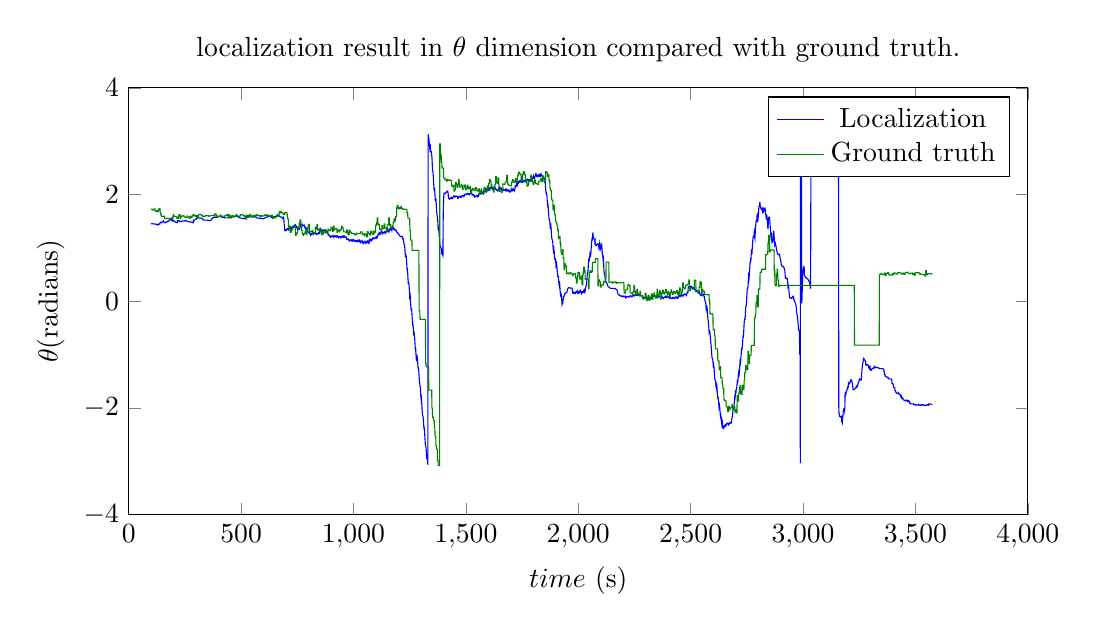
\begin{tikzpicture}

\begin{axis}[
title={localization result in $\theta$ dimension compared with ground truth.},
xlabel={$time$ (s)},
ylabel={$\theta$(radians)},
xmin=0, xmax=4000,
ymin=-4, ymax=4,
axis on top,
width=13cm,
height=7cm,
legend entries={{Localization},{Ground truth}}
]
\addplot [blue]
coordinates {
(100,1.45416832345806)
(101,1.45313839626442)
(102,1.45302394926372)
(103,1.45335578343005)
(104,1.452920065188)
(105,1.45348772598533)
(106,1.45229643112176)
(107,1.45109032594701)
(108,1.45072695888526)
(109,1.45041981681169)
(110,1.45045728872235)
(111,1.44990587436563)
(112,1.44956357730824)
(113,1.44925753900899)
(114,1.45069315370982)
(115,1.4496040292014)
(116,1.44905878734672)
(117,1.44594907687781)
(118,1.44312036368621)
(119,1.43977790211221)
(120,1.4408894323273)
(121,1.43968224260298)
(122,1.44010694732115)
(123,1.44139292719466)
(124,1.4454822742815)
(125,1.44473064923351)
(126,1.44116599950631)
(127,1.43732562544447)
(128,1.43234741571051)
(129,1.42668367805582)
(130,1.42953474307124)
(131,1.43434046255116)
(132,1.43618340002459)
(133,1.44046958260324)
(134,1.44592382870239)
(135,1.45131105761599)
(136,1.45173011063905)
(137,1.44635591325658)
(138,1.44493220707243)
(139,1.4577067454718)
(140,1.46382211407489)
(141,1.47336429632083)
(142,1.47752750066582)
(143,1.4824867862524)
(144,1.47982602685299)
(145,1.47267165594232)
(146,1.47719138117801)
(147,1.47699574883239)
(148,1.48128167424852)
(149,1.48272808742726)
(150,1.48836537589009)
(151,1.49114142218384)
(152,1.49401030083898)
(153,1.49811210286467)
(154,1.50214853656104)
(155,1.50559116080588)
(156,1.49974491372889)
(157,1.48049508367293)
(158,1.47625211047092)
(159,1.47614210481053)
(160,1.47218177604298)
(161,1.47290090632639)
(162,1.47303327349407)
(163,1.47092975978731)
(164,1.47926778550847)
(165,1.47959431931032)
(166,1.48164124844379)
(167,1.48414144536264)
(168,1.48422108228305)
(169,1.48538514527945)
(170,1.48730930358624)
(171,1.48629952968083)
(172,1.48898214486322)
(173,1.49013141758984)
(174,1.50283324671258)
(175,1.50342602533313)
(176,1.49665289038331)
(177,1.50140040897057)
(178,1.50149853272272)
(179,1.50912893290581)
(180,1.51827204422743)
(181,1.51789463386475)
(182,1.51795544402417)
(183,1.52236036665826)
(184,1.5360861479319)
(185,1.53622295375462)
(186,1.53828655111506)
(187,1.53202726747779)
(188,1.53029929817789)
(189,1.53154356888681)
(190,1.53068036102471)
(191,1.52914081205048)
(192,1.50748140987776)
(193,1.50609757409397)
(194,1.52983118025491)
(195,1.50524797214858)
(196,1.50482369525497)
(197,1.50368369769217)
(198,1.51388717969275)
(199,1.51193936122653)
(200,1.50575214032382)
(201,1.50169899261546)
(202,1.50545605631805)
(203,1.50418349837005)
(204,1.49808119683787)
(205,1.49165818293365)
(206,1.492075666538)
(207,1.48295750327607)
(208,1.47838330553725)
(209,1.47945930939956)
(210,1.47739419442615)
(211,1.47643650513385)
(212,1.47598020796343)
(213,1.47442414756621)
(214,1.47420168485922)
(215,1.4774063863067)
(216,1.47531928046243)
(217,1.51285494869537)
(218,1.51127200377876)
(219,1.51050757902475)
(220,1.50870882998423)
(221,1.50806426669851)
(222,1.50908419863752)
(223,1.49944232648903)
(224,1.49899368936881)
(225,1.49560199529941)
(226,1.5002169506688)
(227,1.49637979906129)
(228,1.49595615965073)
(229,1.49524646133505)
(230,1.49659147143611)
(231,1.49479928017527)
(232,1.49350918646221)
(233,1.49349065670023)
(234,1.49301003550505)
(235,1.49226759380876)
(236,1.49155437593138)
(237,1.49234463819991)
(238,1.50276295034595)
(239,1.50324068107097)
(240,1.50571752702752)
(241,1.50601882081238)
(242,1.50654331139389)
(243,1.50598427785667)
(244,1.50571589844395)
(245,1.50573105148047)
(246,1.50430375113413)
(247,1.50473570333166)
(248,1.50350781435396)
(249,1.50668161868251)
(250,1.50784377724673)
(251,1.50462644748388)
(252,1.50970366861045)
(253,1.51463048611779)
(254,1.5155755435389)
(255,1.51383244518761)
(256,1.51293433974041)
(257,1.50885621563502)
(258,1.50673015381087)
(259,1.50304435034449)
(260,1.50011446229997)
(261,1.50040119580575)
(262,1.49662647598203)
(263,1.49496281995937)
(264,1.49366543389528)
(265,1.490628370074)
(266,1.48980901944136)
(267,1.48853789830855)
(268,1.48673569460763)
(269,1.4860468743812)
(270,1.48639217701048)
(271,1.48495573650353)
(272,1.48615835555603)
(273,1.48466641590704)
(274,1.48430857658586)
(275,1.48556454023116)
(276,1.48569903378602)
(277,1.48413201734934)
(278,1.48493067683245)
(279,1.48281208829616)
(280,1.48084214173419)
(281,1.48074776144971)
(282,1.47312250038834)
(283,1.47108668976575)
(284,1.46993507458822)
(285,1.47739561489922)
(286,1.47551245192182)
(287,1.47347024606256)
(288,1.51203471971673)
(289,1.50574875645801)
(290,1.51495434548545)
(291,1.51664691650436)
(292,1.51588360464011)
(293,1.52083228678436)
(294,1.52654255301443)
(295,1.52849409142129)
(296,1.53395538777543)
(297,1.53623048524695)
(298,1.53859423047963)
(299,1.54051920174639)
(300,1.53965592313873)
(301,1.53850069716491)
(302,1.55998461333501)
(303,1.55959680273132)
(304,1.55862641934419)
(305,1.55801657887604)
(306,1.55718322616992)
(307,1.55716198861209)
(308,1.55718908037851)
(309,1.55740904371538)
(310,1.55755215462107)
(311,1.55818572985809)
(312,1.55844545743059)
(313,1.55994210910614)
(314,1.55841424380525)
(315,1.55856611459205)
(316,1.55859971509193)
(317,1.56017791242971)
(318,1.55951551659044)
(319,1.56000594280643)
(320,1.55971797587714)
(321,1.55979132584811)
(322,1.55921658886772)
(323,1.55795743036722)
(324,1.55702391766133)
(325,1.5549404782083)
(326,1.55338108759691)
(327,1.55043176995968)
(328,1.54462960601164)
(329,1.54338861366851)
(330,1.53623233837559)
(331,1.52170255345426)
(332,1.52236706331949)
(333,1.52254292861856)
(334,1.52234379090929)
(335,1.522031067684)
(336,1.52147032241456)
(337,1.5204975175688)
(338,1.52027634863677)
(339,1.52030216287875)
(340,1.52021431104915)
(341,1.51998146586951)
(342,1.52031703344613)
(343,1.52062236599407)
(344,1.52054854396609)
(345,1.52067097401648)
(346,1.52077495447936)
(347,1.52097660723719)
(348,1.51737523755635)
(349,1.51715480013861)
(350,1.51542784882363)
(351,1.51589938476686)
(352,1.51527372621015)
(353,1.51548761516665)
(354,1.51567499719734)
(355,1.51555647454913)
(356,1.51525573869104)
(357,1.5124203845448)
(358,1.51197084899362)
(359,1.51207489551029)
(360,1.51170328252478)
(361,1.51164956673579)
(362,1.51176934227326)
(363,1.51211899474173)
(364,1.51319717867878)
(365,1.51388680278302)
(366,1.52312978144506)
(367,1.52744522626004)
(368,1.53329663757426)
(369,1.5388050554138)
(370,1.54402355158582)
(371,1.54900181223878)
(372,1.55353333442353)
(373,1.55516593541391)
(374,1.56054647497678)
(375,1.56511860923839)
(376,1.56631997807068)
(377,1.56794675555831)
(378,1.57123089332566)
(379,1.57273877102097)
(380,1.57257783486675)
(381,1.5733221125149)
(382,1.57362146473126)
(383,1.57319279111903)
(384,1.57316201774196)
(385,1.57344617318949)
(386,1.5737718286044)
(387,1.57478568919327)
(388,1.57527067559997)
(389,1.57529461680381)
(390,1.5753117604406)
(391,1.57487827678481)
(392,1.57494487834809)
(393,1.57334688498745)
(394,1.58845086076255)
(395,1.58854203383138)
(396,1.58804819598759)
(397,1.58723454011164)
(398,1.58727574797623)
(399,1.58758723284757)
(400,1.586970608873)
(401,1.58714465819698)
(402,1.5870927707899)
(403,1.58693213315964)
(404,1.58690580308132)
(405,1.58714200631969)
(406,1.58689942336586)
(407,1.5864569105301)
(408,1.58628061978957)
(409,1.5861174276272)
(410,1.58433833253459)
(411,1.58279231183317)
(412,1.58180278804507)
(413,1.58031166858051)
(414,1.57560274693907)
(415,1.57403956621861)
(416,1.57155233562378)
(417,1.57143448374532)
(418,1.57188546822125)
(419,1.57252381206304)
(420,1.57226183676166)
(421,1.5720777694822)
(422,1.57196176592169)
(423,1.56932024752411)
(424,1.5694113425571)
(425,1.56865817457369)
(426,1.56866713026433)
(427,1.56823192949647)
(428,1.56341324870353)
(429,1.56184135696243)
(430,1.56194710423081)
(431,1.56190281611449)
(432,1.56191378007509)
(433,1.56183361235086)
(434,1.56165022948831)
(435,1.56149126065827)
(436,1.56161972789739)
(437,1.56326230031837)
(438,1.56317648384281)
(439,1.56299371546799)
(440,1.56277226113107)
(441,1.56275373640987)
(442,1.56257116248039)
(443,1.56257973810072)
(444,1.56132020721244)
(445,1.56204810110901)
(446,1.5637240976784)
(447,1.56526983657132)
(448,1.56701576188644)
(449,1.56856228540281)
(450,1.57073874308369)
(451,1.57905162486195)
(452,1.58209356341544)
(453,1.58324036325722)
(454,1.5840632330466)
(455,1.58475495375773)
(456,1.58582443912901)
(457,1.58621597761539)
(458,1.58703424927791)
(459,1.58711719905454)
(460,1.5865679983657)
(461,1.58744319891166)
(462,1.58872552678264)
(463,1.58868096927319)
(464,1.58868670784336)
(465,1.58879494204402)
(466,1.58908951321433)
(467,1.5891086500225)
(468,1.58912799003989)
(469,1.58911983770955)
(470,1.58912807710309)
(471,1.58913238016126)
(472,1.5890338844978)
(473,1.58932192104065)
(474,1.59016380309704)
(475,1.5909059483043)
(476,1.59126573310662)
(477,1.59228801998934)
(478,1.59254482347229)
(479,1.59386407417162)
(480,1.59471274808933)
(481,1.59461523721695)
(482,1.59502810042312)
(483,1.59403544086793)
(484,1.59245002940927)
(485,1.59006389977012)
(486,1.58751710117004)
(487,1.57833093353667)
(488,1.575015989006)
(489,1.57268584819584)
(490,1.5690623040924)
(491,1.56799631611873)
(492,1.5673917270486)
(493,1.5669193748308)
(494,1.5612310081986)
(495,1.56108234442563)
(496,1.56087443361299)
(497,1.5606707104234)
(498,1.5592425130239)
(499,1.55884143562609)
(500,1.55830654773933)
(501,1.55794903323474)
(502,1.55801282191894)
(503,1.55806900176319)
(504,1.55811764663665)
(505,1.55814368132631)
(506,1.55305475145584)
(507,1.54705434605766)
(508,1.54607667430216)
(509,1.54778851932062)
(510,1.55105802120067)
(511,1.55077377396289)
(512,1.55045386845291)
(513,1.55011831037563)
(514,1.54982551644051)
(515,1.549532019585)
(516,1.54896410225693)
(517,1.54800372430282)
(518,1.54786675101721)
(519,1.5475138314586)
(520,1.54775795504123)
(521,1.54784361924961)
(522,1.54796003159033)
(523,1.54879612296619)
(524,1.54964629930061)
(525,1.5606839109332)
(526,1.56601809537017)
(527,1.57057271933641)
(528,1.57091901918281)
(529,1.57134739594167)
(530,1.57204961248678)
(531,1.57288536626079)
(532,1.57593560521279)
(533,1.57644629984949)
(534,1.5769135962951)
(535,1.5770878151142)
(536,1.58114737389746)
(537,1.58139507156816)
(538,1.58232099418829)
(539,1.58244819071178)
(540,1.58267225215375)
(541,1.58454291465833)
(542,1.58683937327296)
(543,1.59368543331054)
(544,1.59736531880844)
(545,1.59769944779524)
(546,1.59400739638707)
(547,1.59402510725752)
(548,1.59399033981438)
(549,1.59373941956456)
(550,1.59377917470575)
(551,1.59371862609432)
(552,1.5936319551917)
(553,1.59371896060951)
(554,1.59437784592282)
(555,1.5949439814165)
(556,1.59566096954277)
(557,1.59575005221189)
(558,1.59563879263437)
(559,1.59579258812033)
(560,1.59538623881885)
(561,1.59497787977389)
(562,1.59327560848817)
(563,1.5885589438236)
(564,1.58291784916076)
(565,1.5791895721702)
(566,1.5752021196677)
(567,1.57226421547056)
(568,1.56723284723171)
(569,1.56478311434244)
(570,1.56314519069759)
(571,1.56002535092212)
(572,1.55838486268673)
(573,1.55804794940899)
(574,1.5576674344661)
(575,1.5572936038034)
(576,1.55703379845959)
(577,1.55610434870294)
(578,1.55577314630752)
(579,1.55553985825098)
(580,1.55541197515528)
(581,1.55584234429376)
(582,1.55531748593172)
(583,1.55514697955483)
(584,1.55533797625072)
(585,1.55197321133559)
(586,1.55055074537001)
(587,1.55099873362117)
(588,1.55242152634255)
(589,1.55225170840593)
(590,1.55080414944423)
(591,1.55050131183022)
(592,1.55026511021143)
(593,1.54968914941092)
(594,1.54902772482303)
(595,1.5484378884483)
(596,1.54729140049229)
(597,1.5462895307753)
(598,1.54501768105545)
(599,1.54518073008554)
(600,1.54530776868392)
(601,1.54559203679348)
(602,1.54660684544713)
(603,1.55076760596611)
(604,1.55683202344914)
(605,1.5594883472957)
(606,1.56400501672194)
(607,1.56608512381327)
(608,1.56643004390857)
(609,1.56722978509164)
(610,1.56960818485575)
(611,1.57041745314411)
(612,1.57152713655848)
(613,1.57338942775945)
(614,1.57772621453595)
(615,1.57971317110266)
(616,1.58155213949102)
(617,1.58528010533221)
(618,1.58548713310406)
(619,1.58561079716575)
(620,1.58574003291828)
(621,1.58705663365461)
(622,1.58524379819781)
(623,1.584894158557)
(624,1.584800982965)
(625,1.58443316190123)
(626,1.58440859069668)
(627,1.58447146294959)
(628,1.58456655631773)
(629,1.58379073282198)
(630,1.58268182728865)
(631,1.58292882478179)
(632,1.58345525226621)
(633,1.58313077008424)
(634,1.58268636728787)
(635,1.57489942144399)
(636,1.57553985449612)
(637,1.57388587324951)
(638,1.5732645485326)
(639,1.57189402803281)
(640,1.57254340712364)
(641,1.57392970143661)
(642,1.57560888985018)
(643,1.57761388930727)
(644,1.57842871721822)
(645,1.57867475521669)
(646,1.58125392057669)
(647,1.58279142836208)
(648,1.5871060632932)
(649,1.58575829671474)
(650,1.58742047464891)
(651,1.58968436476259)
(652,1.58919361653382)
(653,1.58985917937698)
(654,1.59135280495266)
(655,1.59242749001877)
(656,1.59341215956537)
(657,1.59417282472877)
(658,1.59514800965807)
(659,1.59607167940358)
(660,1.60162875193998)
(661,1.60362763887858)
(662,1.600355679451)
(663,1.6020723250706)
(664,1.60571013265293)
(665,1.6004639856513)
(666,1.60102598570471)
(667,1.59978408087158)
(668,1.60090775734033)
(669,1.59950647827449)
(670,1.59177827794971)
(671,1.58610516512203)
(672,1.5865310424078)
(673,1.58519044663976)
(674,1.58601894595301)
(675,1.58384851552599)
(676,1.5783052239644)
(677,1.5768980718802)
(678,1.57536027836795)
(679,1.57343583833964)
(680,1.57431208019351)
(681,1.5724772050763)
(682,1.57067094903545)
(683,1.56830502445826)
(684,1.56243629233507)
(685,1.55547322447795)
(686,1.56838333244377)
(687,1.5641188938697)
(688,1.55518370083594)
(689,1.56669608726258)
(690,1.54970873955672)
(691,1.49277614492958)
(692,1.43020050663536)
(693,1.38296497676556)
(694,1.34096294704859)
(695,1.34830166928505)
(696,1.3350307733569)
(697,1.31806556393113)
(698,1.31796102415084)
(699,1.32176067415718)
(700,1.33322213663632)
(701,1.32862635449418)
(702,1.33262575788088)
(703,1.3351224881125)
(704,1.35030166229852)
(705,1.34942035556119)
(706,1.34812496358398)
(707,1.36102788156601)
(708,1.36238418867641)
(709,1.35464683181893)
(710,1.34376769904331)
(711,1.33873160702319)
(712,1.3463410814959)
(713,1.36117832229616)
(714,1.37117232994319)
(715,1.37722215016516)
(716,1.3880543751377)
(717,1.38800584948404)
(718,1.39092048586706)
(719,1.39478322331222)
(720,1.39658018682046)
(721,1.38374802950663)
(722,1.3578772946809)
(723,1.35954570994606)
(724,1.3571952217341)
(725,1.36918451814806)
(726,1.37864377000112)
(727,1.38201146433388)
(728,1.39027218049047)
(729,1.39717753131196)
(730,1.39692618262483)
(731,1.40965695616318)
(732,1.41029858939577)
(733,1.40440183250461)
(734,1.39369035501908)
(735,1.38472468241917)
(736,1.38646714639997)
(737,1.39859077398813)
(738,1.41153603358493)
(739,1.41429421256181)
(740,1.43617932272258)
(741,1.4381264051853)
(742,1.42179736005911)
(743,1.42181203689125)
(744,1.41727284000128)
(745,1.41249435665944)
(746,1.3834224124948)
(747,1.37709748144695)
(748,1.37267362926388)
(749,1.37253487853427)
(750,1.36357122005989)
(751,1.37507745528687)
(752,1.36666980197747)
(753,1.36063066169713)
(754,1.3583176478101)
(755,1.35771840669309)
(756,1.35945343352482)
(757,1.35521209127261)
(758,1.35901626863166)
(759,1.35708394112309)
(760,1.35184294801449)
(761,1.36312569841986)
(762,1.37885510526841)
(763,1.39134818388662)
(764,1.39562885908923)
(765,1.42458367607138)
(766,1.41906538877539)
(767,1.41784518512426)
(768,1.41784072371863)
(769,1.40882589279406)
(770,1.42415263270329)
(771,1.44105533090722)
(772,1.42567430251939)
(773,1.42135700247785)
(774,1.41694181716109)
(775,1.41441275709996)
(776,1.41857524700219)
(777,1.42191220832683)
(778,1.42292695447032)
(779,1.41863105019134)
(780,1.42911760566453)
(781,1.41561452999187)
(782,1.40250501920627)
(783,1.39238732912736)
(784,1.39061708631152)
(785,1.37317431221424)
(786,1.37742662026254)
(787,1.38274453549353)
(788,1.36863339982835)
(789,1.37133363086638)
(790,1.37019210698732)
(791,1.35081931045027)
(792,1.3374911835185)
(793,1.3367051152636)
(794,1.33467420409033)
(795,1.32594608599207)
(796,1.31491562994084)
(797,1.29887600313759)
(798,1.28994716582231)
(799,1.2929199749545)
(800,1.28648137552075)
(801,1.28518752285916)
(802,1.28972819590569)
(803,1.29655084498167)
(804,1.26727983697977)
(805,1.26427049276147)
(806,1.27777742028896)
(807,1.27015150022189)
(808,1.25265826287531)
(809,1.24765543188262)
(810,1.23622789128076)
(811,1.24917714937649)
(812,1.25147843005982)
(813,1.25431282370266)
(814,1.26620585755963)
(815,1.27278672955516)
(816,1.26405982631776)
(817,1.26565319793816)
(818,1.27904737010695)
(819,1.28245257118831)
(820,1.26641286090072)
(821,1.2503888841724)
(822,1.25310979941915)
(823,1.25919734257523)
(824,1.27076443786982)
(825,1.27388303903181)
(826,1.28179665644903)
(827,1.28244567000217)
(828,1.28235005234481)
(829,1.27556832311822)
(830,1.27280885717047)
(831,1.28421754879382)
(832,1.27635575290558)
(833,1.26236312575427)
(834,1.26185629884501)
(835,1.2531842449545)
(836,1.25876023628993)
(837,1.25743695217429)
(838,1.25606249959324)
(839,1.2694530348429)
(840,1.27115135661893)
(841,1.26763220939866)
(842,1.26664535007986)
(843,1.2747809426448)
(844,1.28289528615387)
(845,1.28376900485564)
(846,1.26541018618649)
(847,1.2640239665922)
(848,1.27219099809455)
(849,1.28850825761484)
(850,1.35190798986983)
(851,1.35884635747244)
(852,1.36764995605518)
(853,1.36438947255557)
(854,1.33426768458587)
(855,1.33488982043924)
(856,1.33889612392746)
(857,1.32867875606518)
(858,1.31526304972123)
(859,1.31350989772238)
(860,1.31428827195304)
(861,1.32346115204382)
(862,1.32902951528194)
(863,1.32972025363628)
(864,1.34018849915054)
(865,1.33488780632072)
(866,1.32936676358261)
(867,1.32885936906477)
(868,1.32312386425349)
(869,1.32648172170595)
(870,1.32292379682623)
(871,1.31835920124786)
(872,1.31629871936818)
(873,1.32725092774947)
(874,1.31699139964245)
(875,1.29841245261993)
(876,1.31099488887955)
(877,1.31640781950225)
(878,1.31285323737209)
(879,1.29774782930677)
(880,1.29843755313037)
(881,1.2970414350686)
(882,1.29069730527153)
(883,1.27668427586282)
(884,1.27716278331896)
(885,1.28030777004582)
(886,1.26949324020219)
(887,1.24953497429635)
(888,1.25658690443989)
(889,1.25799783229007)
(890,1.25502053818445)
(891,1.23970101511353)
(892,1.23584437767966)
(893,1.23481714983461)
(894,1.22680999203011)
(895,1.21491634131089)
(896,1.21624168330018)
(897,1.21920438867133)
(898,1.20517749210599)
(899,1.19858923658114)
(900,1.20137808272932)
(901,1.21108080644971)
(902,1.2157552282244)
(903,1.21346898654678)
(904,1.21333093688611)
(905,1.22045367444519)
(906,1.22510242323045)
(907,1.21458724188272)
(908,1.20891846949739)
(909,1.21203404735347)
(910,1.2204388303267)
(911,1.21081355222063)
(912,1.20100380259883)
(913,1.21157876181733)
(914,1.22198465653348)
(915,1.22645205991576)
(916,1.22146625338356)
(917,1.21784060793643)
(918,1.21398274596495)
(919,1.22075229252697)
(920,1.20788692425013)
(921,1.20648828882894)
(922,1.21250984247944)
(923,1.21607464797034)
(924,1.20782555046662)
(925,1.21365717978658)
(926,1.22760806755542)
(927,1.2246955908966)
(928,1.21223407760612)
(929,1.21866991809952)
(930,1.20940360073939)
(931,1.20401791316464)
(932,1.20157492110513)
(933,1.19429881760269)
(934,1.19771670437407)
(935,1.20618715955865)
(936,1.19623033682805)
(937,1.19953917604024)
(938,1.20995247328363)
(939,1.20945985907552)
(940,1.21380520260574)
(941,1.21175876211056)
(942,1.20752736504802)
(943,1.20477337032928)
(944,1.18539185615123)
(945,1.18773684306053)
(946,1.19539762280813)
(947,1.20737594358555)
(948,1.20171300267732)
(949,1.1983433623512)
(950,1.21012197672137)
(951,1.21796818654634)
(952,1.22095873160303)
(953,1.21698415999141)
(954,1.22226084234118)
(955,1.21324776144112)
(956,1.19932820399637)
(957,1.19894302276693)
(958,1.20356569660404)
(959,1.21531826385805)
(960,1.20370299814856)
(961,1.20098527375873)
(962,1.1995356887511)
(963,1.20559966744726)
(964,1.20328310634659)
(965,1.20348813958621)
(966,1.20275213328918)
(967,1.20537947402374)
(968,1.17883970900892)
(969,1.17744365627296)
(970,1.16009209047395)
(971,1.16229966515632)
(972,1.16151490976292)
(973,1.15937099653202)
(974,1.16777796782119)
(975,1.171705688259)
(976,1.16628741067352)
(977,1.16333466263782)
(978,1.16346608056129)
(979,1.15554607163)
(980,1.1355258618359)
(981,1.12636779928058)
(982,1.13094077142579)
(983,1.14009452401352)
(984,1.13413900628352)
(985,1.13589200519622)
(986,1.14626385887355)
(987,1.14264176938381)
(988,1.14026291090327)
(989,1.14180597866444)
(990,1.14779245346313)
(991,1.13489443301683)
(992,1.12754516980436)
(993,1.1283825945911)
(994,1.12806883507676)
(995,1.14046837771478)
(996,1.13094518995079)
(997,1.14141965652141)
(998,1.14910208888957)
(999,1.14118374311129)
(1000,1.13976171773041)
(1001,1.14281080253761)
(1002,1.14691447373956)
(1003,1.13045583866361)
(1004,1.12267995034437)
(1005,1.12286144572731)
(1006,1.12846061792522)
(1007,1.12995944354049)
(1008,1.12191220544735)
(1009,1.12573779569463)
(1010,1.13947767437584)
(1011,1.13931301604452)
(1012,1.12989476053691)
(1013,1.13286722591774)
(1014,1.13361728251632)
(1015,1.12678152541912)
(1016,1.11289940062261)
(1017,1.11164564660309)
(1018,1.11675289490583)
(1019,1.13207200386885)
(1020,1.12255697550406)
(1021,1.12534080880848)
(1022,1.13830007992617)
(1023,1.14170292149659)
(1024,1.12528546123993)
(1025,1.12998786726682)
(1026,1.13983218475727)
(1027,1.12977468584695)
(1028,1.11491401762732)
(1029,1.10640670091925)
(1030,1.10666510603004)
(1031,1.11584460753269)
(1032,1.09509509633548)
(1033,1.0959575020291)
(1034,1.11207572860197)
(1035,1.12197698076214)
(1036,1.11737576342146)
(1037,1.12015776030458)
(1038,1.11769987243898)
(1039,1.12799972083158)
(1040,1.11333516973204)
(1041,1.09615994605368)
(1042,1.10097732047881)
(1043,1.1041038033303)
(1044,1.10028568461837)
(1045,1.08591011438818)
(1046,1.0916224741832)
(1047,1.10950770466482)
(1048,1.10736074512718)
(1049,1.10827161102682)
(1050,1.11545041027606)
(1051,1.12333816114009)
(1052,1.11472402157628)
(1053,1.08923309499764)
(1054,1.09271784935512)
(1055,1.09287335043731)
(1056,1.10503938114229)
(1057,1.08793913824442)
(1058,1.0878048320124)
(1059,1.10430726111543)
(1060,1.10908875829217)
(1061,1.10508904075858)
(1062,1.11001348058369)
(1063,1.12879381077972)
(1064,1.12696019611929)
(1065,1.10687099892444)
(1066,1.09708896308935)
(1067,1.09013628650749)
(1068,1.10213037117096)
(1069,1.1229696674523)
(1070,1.10731386937625)
(1071,1.12185160602868)
(1072,1.14240540351212)
(1073,1.13457908734173)
(1074,1.13743093477644)
(1075,1.13694156283129)
(1076,1.16135323183227)
(1077,1.15766151243273)
(1078,1.13751728454057)
(1079,1.12908413441304)
(1080,1.13254971149836)
(1081,1.14776926616129)
(1082,1.15911955177952)
(1083,1.15606104059263)
(1084,1.17956465704485)
(1085,1.18343151023729)
(1086,1.18597837608483)
(1087,1.18532766142932)
(1088,1.18745686116171)
(1089,1.18818605117392)
(1090,1.16879553705346)
(1091,1.16989974767327)
(1092,1.17111704225332)
(1093,1.18044743413717)
(1094,1.17590825359017)
(1095,1.17548482842191)
(1096,1.18242633740773)
(1097,1.18994962970515)
(1098,1.19207708261865)
(1099,1.19257229046388)
(1100,1.18759522160008)
(1101,1.21176961754872)
(1102,1.21006079927956)
(1103,1.18329807908212)
(1104,1.18736185996731)
(1105,1.18779391230079)
(1106,1.19995920446696)
(1107,1.22091094880475)
(1108,1.22134539410931)
(1109,1.24975749066833)
(1110,1.24645602920826)
(1111,1.25121559792932)
(1112,1.25066849254107)
(1113,1.27452331259882)
(1114,1.28188845971635)
(1115,1.26883681202343)
(1116,1.25103700803628)
(1117,1.24767290893906)
(1118,1.24843329796531)
(1119,1.26846814947166)
(1120,1.27834310987928)
(1121,1.28982944460549)
(1122,1.29816295745141)
(1123,1.29436704798891)
(1124,1.29777267207522)
(1125,1.29793320830172)
(1126,1.30330011156579)
(1127,1.3021371882754)
(1128,1.26030370931799)
(1129,1.26027254314645)
(1130,1.26378736255639)
(1131,1.26812867636869)
(1132,1.28606056437704)
(1133,1.28626239607841)
(1134,1.28661704628779)
(1135,1.28831159120476)
(1136,1.29111162370121)
(1137,1.30130087567543)
(1138,1.29810131727405)
(1139,1.29276187368911)
(1140,1.29685854124589)
(1141,1.27158663752241)
(1142,1.27761660194708)
(1143,1.27947314076344)
(1144,1.28851546246776)
(1145,1.30765055824188)
(1146,1.31393709179388)
(1147,1.32551944215225)
(1148,1.31927431494342)
(1149,1.31588793678023)
(1150,1.32561099102534)
(1151,1.34104397368198)
(1152,1.32248747755354)
(1153,1.30695316322659)
(1154,1.31126354016875)
(1155,1.31154811728896)
(1156,1.31730796016041)
(1157,1.32788384883884)
(1158,1.3083441275287)
(1159,1.33231430492583)
(1160,1.34314761675182)
(1161,1.33369845412635)
(1162,1.34249865431302)
(1163,1.35183154679798)
(1164,1.36525083035194)
(1165,1.35368547569924)
(1166,1.33928033504599)
(1167,1.33534333463722)
(1168,1.33476358522857)
(1169,1.34766454958553)
(1170,1.35712490380938)
(1171,1.33646211923296)
(1172,1.3666411373877)
(1173,1.38262558133538)
(1174,1.37212247831012)
(1175,1.374874588905)
(1176,1.38710022425475)
(1177,1.38200537149059)
(1178,1.38009411712374)
(1179,1.35389916725322)
(1180,1.35856697508931)
(1181,1.36041522699739)
(1182,1.35044279064383)
(1183,1.34554667559783)
(1184,1.33324447715055)
(1185,1.32830323439164)
(1186,1.33335793038199)
(1187,1.32777577425653)
(1188,1.32375003347887)
(1189,1.32847711564174)
(1190,1.31732701940754)
(1191,1.31255195306318)
(1192,1.30681693384128)
(1193,1.29771793425121)
(1194,1.28611621122856)
(1195,1.28157770046795)
(1196,1.28283492168242)
(1197,1.26965531713434)
(1198,1.26543545773763)
(1199,1.26944845931437)
(1200,1.26103743248461)
(1201,1.25366536464067)
(1202,1.25228829492762)
(1203,1.25200368727158)
(1204,1.23759240787417)
(1205,1.23023381535591)
(1206,1.22580332572161)
(1207,1.22147330986479)
(1208,1.21968280529179)
(1209,1.21134880805437)
(1210,1.21316472843232)
(1211,1.21324639593629)
(1212,1.21364977571107)
(1213,1.21088946044432)
(1214,1.21219743322821)
(1215,1.21240897485206)
(1216,1.21195584997257)
(1217,1.21161433642564)
(1218,1.18562815699461)
(1219,1.18638950682981)
(1220,1.1581751952411)
(1221,1.16033466960437)
(1222,1.16214069216117)
(1223,1.13305076492812)
(1224,1.09477915907753)
(1225,1.06605696356518)
(1226,1.05698514852463)
(1227,1.05813376931758)
(1228,1.01479600172578)
(1229,0.963056325070401)
(1230,0.912158045145812)
(1231,0.842612195783068)
(1232,0.848113841865916)
(1233,0.868173294148246)
(1234,0.861882981795115)
(1235,0.830614844897526)
(1236,0.745171061258889)
(1237,0.697901855625901)
(1238,0.619185120593594)
(1239,0.579027815860492)
(1240,0.587286533556735)
(1241,0.543259282405729)
(1242,0.464377198917858)
(1243,0.37804069813953)
(1244,0.31991807088371)
(1245,0.35531625288993)
(1246,0.347840912587981)
(1247,0.310757164496896)
(1248,0.251653261207139)
(1249,0.189536124301779)
(1250,0.0932988170697513)
(1251,0.109874200385531)
(1252,0.117487901016208)
(1253,0.0670069019636839)
(1254,-0.0191515226521766)
(1255,-0.095227375113196)
(1256,-0.14594070747196)
(1257,-0.137948477570219)
(1258,-0.136944623442808)
(1259,-0.172206107455038)
(1260,-0.216577802935257)
(1261,-0.300903054990023)
(1262,-0.360938831709205)
(1263,-0.423465175649571)
(1264,-0.413294977545506)
(1265,-0.459629943585462)
(1266,-0.499649379187288)
(1267,-0.576475161843957)
(1268,-0.638792442220407)
(1269,-0.606001909368392)
(1270,-0.598258036478278)
(1271,-0.633804394347023)
(1272,-0.68665883227845)
(1273,-0.743943777763098)
(1274,-0.817414802581816)
(1275,-0.891670252652757)
(1276,-0.918200773643248)
(1277,-0.911881863599577)
(1278,-0.987674048607423)
(1279,-1.05014344539444)
(1280,-1.12550299360739)
(1281,-1.07395173013285)
(1282,-1.03704384163038)
(1283,-1.0292885077861)
(1284,-1.06205968982403)
(1285,-1.09057889463686)
(1286,-1.16522682251586)
(1287,-1.24125679928542)
(1288,-1.26347265483223)
(1289,-1.2579734354628)
(1290,-1.29479633594233)
(1291,-1.35430626019417)
(1292,-1.41328873306095)
(1293,-1.47302597501553)
(1294,-1.53724456954338)
(1295,-1.54892800845821)
(1296,-1.58947365244644)
(1297,-1.60247452173467)
(1298,-1.6595207786941)
(1299,-1.74367434892888)
(1300,-1.80088709283705)
(1301,-1.83800489816899)
(1302,-1.81603571388955)
(1303,-1.87196041308696)
(1304,-1.94087444732285)
(1305,-2.02289433143084)
(1306,-2.0823469034269)
(1307,-2.13322229298559)
(1308,-2.14225512249416)
(1309,-2.15403569051003)
(1310,-2.17330667543305)
(1311,-2.23115936460985)
(1312,-2.29290795336802)
(1313,-2.36627477840951)
(1314,-2.38769756132236)
(1315,-2.38031911250615)
(1316,-2.41752993513374)
(1317,-2.50634097337271)
(1318,-2.57097403734471)
(1319,-2.64190894855557)
(1320,-2.70087605459986)
(1321,-2.71459619911758)
(1322,-2.72901648713396)
(1323,-2.74728093915987)
(1324,-2.82399398319379)
(1325,-2.89294256516752)
(1326,-2.95943716535985)
(1327,-2.90761299889555)
(1328,-2.89203033838092)
(1329,-2.92806218036294)
(1330,-3.01519664593816)
(1331,-3.07220407047153)
(1332,3.13437292904843)
(1333,3.08586469100107)
(1334,3.06846868240618)
(1335,3.06543982072187)
(1336,3.03784643317255)
(1337,2.97871904553807)
(1338,2.9323111361854)
(1339,2.87875781898117)
(1340,2.90261471099786)
(1341,2.94516368160947)
(1342,2.89772661437952)
(1343,2.83321822954665)
(1344,2.80017881501729)
(1345,2.78905325763282)
(1346,2.78377058793082)
(1347,2.78849773638174)
(1348,2.73992777704917)
(1349,2.70407410423964)
(1350,2.61410039110094)
(1351,2.52302598942991)
(1352,2.45901074338391)
(1353,2.42386987753164)
(1354,2.40876098398483)
(1355,2.35501947302735)
(1356,2.26447590489304)
(1357,2.19075566898503)
(1358,2.11938631780394)
(1359,2.08274378402069)
(1360,2.06822463737711)
(1361,2.0829949622782)
(1362,2.04067215898951)
(1363,1.95885731203546)
(1364,1.89466987460913)
(1365,1.90087802293717)
(1366,1.91676283585846)
(1367,1.90827841828584)
(1368,1.83714831392288)
(1369,1.77101483712911)
(1370,1.69287336389541)
(1371,1.63871023203253)
(1372,1.60073027531623)
(1373,1.59193936262489)
(1374,1.54290608120766)
(1375,1.50162652468372)
(1376,1.41322681272908)
(1377,1.34348872648577)
(1378,1.34135090601655)
(1379,1.35278160166952)
(1380,1.31306901053434)
(1381,1.26962045972948)
(1382,1.19833163564805)
(1383,1.13343753407205)
(1384,1.06795649717058)
(1385,1.03913298177029)
(1386,1.03672034727528)
(1387,1.0322563393917)
(1388,1.01355681771539)
(1389,1.00265729149143)
(1390,0.996988664724117)
(1391,0.971277182058148)
(1392,0.925641619631397)
(1393,0.935663299837877)
(1394,0.899399815904444)
(1395,0.874663020837078)
(1396,0.867478362626944)
(1397,0.864968784369019)
(1398,0.853212597007123)
(1399,1.49718191554493)
(1400,1.80811158664656)
(1401,1.90608844888524)
(1402,1.98559197022746)
(1403,2.02277526510828)
(1404,2.01623217356232)
(1405,2.01578668232482)
(1406,2.01477261434742)
(1407,2.01530857741206)
(1408,2.01576796901347)
(1409,2.02133462243482)
(1410,2.0252429972913)
(1411,2.03629833142374)
(1412,2.03907975176068)
(1413,2.0429321352414)
(1414,2.04624476901665)
(1415,2.05499245683093)
(1416,2.06221472390042)
(1417,2.06666681224452)
(1418,2.06423852179145)
(1419,2.06157357492174)
(1420,2.05141503800531)
(1421,2.02727654527574)
(1422,1.96800989981442)
(1423,1.9337931674551)
(1424,1.92845005110091)
(1425,1.92623825273752)
(1426,1.91890183955004)
(1427,1.91153402905701)
(1428,1.91856776820197)
(1429,1.92438343840107)
(1430,1.93019716267416)
(1431,1.92597580710409)
(1432,1.92550191343799)
(1433,1.93574052178338)
(1434,1.93813346990025)
(1435,1.93221477449953)
(1436,1.93674582375077)
(1437,1.94172626897543)
(1438,1.93222557124659)
(1439,1.91953360263674)
(1440,1.92055017592682)
(1441,1.92570466625999)
(1442,1.9435419355265)
(1443,1.95357621652172)
(1444,1.95745004549154)
(1445,1.97316060423382)
(1446,1.97237545280943)
(1447,1.96978190328235)
(1448,1.97027790902802)
(1449,1.97199834524489)
(1450,1.96278581252364)
(1451,1.95050191595625)
(1452,1.95157409261938)
(1453,1.95480538420289)
(1454,1.95904937701119)
(1455,1.96889285218232)
(1456,1.96528677993433)
(1457,1.97003045369911)
(1458,1.96674356701216)
(1459,1.96242047891385)
(1460,1.95872586491805)
(1461,1.95708125763394)
(1462,1.96073586543844)
(1463,1.95159540174581)
(1464,1.93257384782709)
(1465,1.9377098833534)
(1466,1.93375749406137)
(1467,1.94406397004411)
(1468,1.95723074114617)
(1469,1.95919329462309)
(1470,1.96251310280687)
(1471,1.96882728033861)
(1472,1.96660800722408)
(1473,1.95972962333315)
(1474,1.96413342217409)
(1475,1.96609952142888)
(1476,1.95705705164426)
(1477,1.94316417286598)
(1478,1.94113458558411)
(1479,1.94616363901139)
(1480,1.95455282419414)
(1481,1.96533901668579)
(1482,1.9683763057036)
(1483,1.97947723586538)
(1484,1.97951033063135)
(1485,1.97702214451408)
(1486,1.97586433430104)
(1487,1.98373362821429)
(1488,1.97804200396775)
(1489,1.96215651676892)
(1490,1.95975574419601)
(1491,1.96194144104786)
(1492,1.96730590950325)
(1493,1.97436775838584)
(1494,1.99258347955625)
(1495,1.99450348253455)
(1496,2.00565623975006)
(1497,2.00478236625767)
(1498,1.99916159341393)
(1499,2.00462529939551)
(1500,2.0078392226258)
(1501,2.00505076513838)
(1502,2.00061088801379)
(1503,2.00207620924453)
(1504,2.00592738759125)
(1505,2.01593170322707)
(1506,2.00838453882933)
(1507,2.00939130245081)
(1508,2.01911795532635)
(1509,2.01824170581242)
(1510,2.01131822478526)
(1511,2.01052752413773)
(1512,2.0183033885312)
(1513,2.01529306745267)
(1514,1.9943439066545)
(1515,1.99334110146341)
(1516,1.99588727807594)
(1517,2.00060370924981)
(1518,2.0145760976885)
(1519,2.01506851246859)
(1520,2.02196795319422)
(1521,2.02667889197572)
(1522,2.02633281810482)
(1523,2.02775826417493)
(1524,2.03501972663906)
(1525,2.0375444136209)
(1526,2.01905537002773)
(1527,2.00340610534937)
(1528,1.9963600916539)
(1529,1.99317626292651)
(1530,1.99728431495638)
(1531,1.98925533057852)
(1532,1.98540456535433)
(1533,1.98815263310671)
(1534,1.99427692386948)
(1535,1.98718236654101)
(1536,1.97410930637525)
(1537,1.97225631397517)
(1538,1.9748323023908)
(1539,1.9534556162201)
(1540,1.95044618748428)
(1541,1.9515957240604)
(1542,1.95691908473448)
(1543,1.96218334740327)
(1544,1.96683147359939)
(1545,1.96492008197886)
(1546,1.97300812682328)
(1547,1.98147393414403)
(1548,1.9784276960476)
(1549,1.97467512862346)
(1550,1.98125558385214)
(1551,1.97744343841037)
(1552,1.95942784914468)
(1553,1.95576051174629)
(1554,1.95771027846498)
(1555,1.96018364080025)
(1556,1.98139712061735)
(1557,2.00003369558605)
(1558,1.99746295396755)
(1559,2.02014263937729)
(1560,2.01751532018664)
(1561,2.0227679130581)
(1562,2.02449530317401)
(1563,2.04784805095707)
(1564,2.05443458492821)
(1565,2.02923957381543)
(1566,2.0149595200285)
(1567,2.00733114494578)
(1568,2.00715604687794)
(1569,2.01764784136762)
(1570,2.03969082038199)
(1571,2.02268603609275)
(1572,2.02571374646019)
(1573,2.02303307040226)
(1574,2.02018041959319)
(1575,2.02859729672137)
(1576,2.05040134446982)
(1577,2.0575389497512)
(1578,2.02051551400836)
(1579,2.01357242403989)
(1580,2.02756997433002)
(1581,2.04848583427056)
(1582,2.06189724698049)
(1583,2.0607543000924)
(1584,2.0684696985)
(1585,2.06836703718279)
(1586,2.05740186311875)
(1587,2.0533382098252)
(1588,2.05245400662095)
(1589,2.04861266923116)
(1590,2.04399126398105)
(1591,2.05056969142939)
(1592,2.05346912658372)
(1593,2.06203009468958)
(1594,2.07689551100093)
(1595,2.08371216076996)
(1596,2.09795150046291)
(1597,2.09673796862409)
(1598,2.08970385124432)
(1599,2.10026513399081)
(1600,2.12222925187545)
(1601,2.11580637931699)
(1602,2.08519989967645)
(1603,2.08928715248783)
(1604,2.09306663297156)
(1605,2.10248884367991)
(1606,2.11310584186855)
(1607,2.10013240766958)
(1608,2.12920230858616)
(1609,2.12692822537973)
(1610,2.12514971940435)
(1611,2.12444826405252)
(1612,2.13862000187343)
(1613,2.12396570831811)
(1614,2.11919623299786)
(1615,2.11222707405142)
(1616,2.11646391925342)
(1617,2.12588938656024)
(1618,2.11532047474975)
(1619,2.11062439521993)
(1620,2.11728919170626)
(1621,2.12615798662717)
(1622,2.1257551018907)
(1623,2.12930383046545)
(1624,2.12343254897199)
(1625,2.13257548424802)
(1626,2.10830112340663)
(1627,2.09925026271583)
(1628,2.10907468024732)
(1629,2.11734431900175)
(1630,2.11296973109336)
(1631,2.12368661872821)
(1632,2.11659748196729)
(1633,2.11021431211727)
(1634,2.09978997721672)
(1635,2.08617457650166)
(1636,2.08644001004199)
(1637,2.09149878150697)
(1638,2.08940656744514)
(1639,2.08579113316361)
(1640,2.07417115908614)
(1641,2.07644186531691)
(1642,2.07126616743436)
(1643,2.07656268087258)
(1644,2.08524026312908)
(1645,2.10259745419999)
(1646,2.11543688449387)
(1647,2.12413152112935)
(1648,2.11446649852518)
(1649,2.11454822233577)
(1650,2.13009735866148)
(1651,2.14084253937766)
(1652,2.12826331996188)
(1653,2.09686989628539)
(1654,2.09980047156863)
(1655,2.10490381939166)
(1656,2.11147279280998)
(1657,2.08594794746317)
(1658,2.08496996341568)
(1659,2.10389309830325)
(1660,2.11026080127167)
(1661,2.10317244275766)
(1662,2.10611216164906)
(1663,2.1079110364418)
(1664,2.11190066475076)
(1665,2.09036971443929)
(1666,2.07799429820516)
(1667,2.08456461386997)
(1668,2.08708388966908)
(1669,2.09145493156676)
(1670,2.08191085807801)
(1671,2.07995066621941)
(1672,2.08432112848857)
(1673,2.08523866435553)
(1674,2.07444319005527)
(1675,2.07408526826113)
(1676,2.08769978753412)
(1677,2.09690559447865)
(1678,2.07309711889486)
(1679,2.06652071631636)
(1680,2.06798634167883)
(1681,2.07092299570452)
(1682,2.08239134472917)
(1683,2.06304576506029)
(1684,2.06318489816279)
(1685,2.08814564507339)
(1686,2.08629503982957)
(1687,2.07773344681741)
(1688,2.07681557358851)
(1689,2.08417903946593)
(1690,2.08487725959571)
(1691,2.06633811214419)
(1692,2.05429769636543)
(1693,2.05356623450938)
(1694,2.05362054979956)
(1695,2.06363408076172)
(1696,2.04531781556612)
(1697,2.04467348074136)
(1698,2.06406903890488)
(1699,2.06418385748143)
(1700,2.06450681615374)
(1701,2.07249278615913)
(1702,2.09731318469843)
(1703,2.10482569638392)
(1704,2.08501993472658)
(1705,2.06593911330186)
(1706,2.06630960563887)
(1707,2.06926070758272)
(1708,2.08420050341361)
(1709,2.10022772375905)
(1710,2.10908291506635)
(1711,2.08801861835207)
(1712,2.0882671668104)
(1713,2.08010896918393)
(1714,2.07919583668466)
(1715,2.08710896567747)
(1716,2.08331351110429)
(1717,2.07158724593266)
(1718,2.08920760811368)
(1719,2.15697225012715)
(1720,2.16424117018868)
(1721,2.15475544609685)
(1722,2.15079465880819)
(1723,2.17106859815314)
(1724,2.17612399620151)
(1725,2.17240590060277)
(1726,2.20056081628073)
(1727,2.19266640581555)
(1728,2.2123554144996)
(1729,2.18649797644893)
(1730,2.17478778571331)
(1731,2.20792749388828)
(1732,2.22166962642507)
(1733,2.23106366877795)
(1734,2.22442666163836)
(1735,2.24422477635703)
(1736,2.24622738105918)
(1737,2.2360834142516)
(1738,2.24022026232704)
(1739,2.25173923503724)
(1740,2.24147890096032)
(1741,2.23311554219535)
(1742,2.23666662145192)
(1743,2.25063799933803)
(1744,2.25997065008785)
(1745,2.23888095172555)
(1746,2.23469682766558)
(1747,2.24929766618184)
(1748,2.2525807974923)
(1749,2.25105663499699)
(1750,2.25007903390762)
(1751,2.24396055472282)
(1752,2.26836252709855)
(1753,2.22931807445462)
(1754,2.22890223684547)
(1755,2.244437934211)
(1756,2.24818225276593)
(1757,2.23824197714154)
(1758,2.23764690818965)
(1759,2.25627090399953)
(1760,2.25948582736282)
(1761,2.25568549953204)
(1762,2.26146490492507)
(1763,2.27052961143607)
(1764,2.26095895042266)
(1765,2.25496378738227)
(1766,2.24315087741947)
(1767,2.24574156491395)
(1768,2.25156228523357)
(1769,2.24158087649257)
(1770,2.26228681278076)
(1771,2.27848872793657)
(1772,2.27927774225562)
(1773,2.2775625377157)
(1774,2.28036582751025)
(1775,2.28741837623584)
(1776,2.28224718563148)
(1777,2.25765490275237)
(1778,2.25810539681127)
(1779,2.26422590208833)
(1780,2.27265400167421)
(1781,2.27772744948982)
(1782,2.27499490812423)
(1783,2.27334609451428)
(1784,2.27063232367583)
(1785,2.26508781913917)
(1786,2.27315877336408)
(1787,2.27796899625431)
(1788,2.28066723286505)
(1789,2.27830264559347)
(1790,2.26650334980358)
(1791,2.26192221803538)
(1792,2.25452724442164)
(1793,2.25880811257399)
(1794,2.27040951686091)
(1795,2.29361705282814)
(1796,2.31127074720449)
(1797,2.31898723110668)
(1798,2.30736759152374)
(1799,2.30752428510628)
(1800,2.31524144421734)
(1801,2.34075345593907)
(1802,2.3221798625908)
(1803,2.29535284015752)
(1804,2.29382575309306)
(1805,2.29661905259296)
(1806,2.310065827858)
(1807,2.33029348362639)
(1808,2.33634644892469)
(1809,2.36023614142492)
(1810,2.37535031844332)
(1811,2.35992478073045)
(1812,2.36362734210148)
(1813,2.36813971219986)
(1814,2.37342879601225)
(1815,2.3406305318366)
(1816,2.33685840392887)
(1817,2.33902898157417)
(1818,2.34388800250768)
(1819,2.34928177396238)
(1820,2.33405328454852)
(1821,2.33742709324166)
(1822,2.35732312553033)
(1823,2.35157544264972)
(1824,2.34934458538361)
(1825,2.35185033205367)
(1826,2.37699479987899)
(1827,2.3708572406886)
(1828,2.33859406603555)
(1829,2.33579316810759)
(1830,2.33504414575695)
(1831,2.3444455919653)
(1832,2.36074239964186)
(1833,2.34788153710364)
(1834,2.35009078163242)
(1835,2.37712964996172)
(1836,2.36356295453351)
(1837,2.36006318306517)
(1838,2.3551621432636)
(1839,2.35000949075781)
(1840,2.34412807787173)
(1841,2.3295535482686)
(1842,2.33101765394546)
(1843,2.32748969405446)
(1844,2.3404927006838)
(1845,2.33088576280597)
(1846,2.3228619708595)
(1847,2.32423574138983)
(1848,2.30506774704633)
(1849,2.27293161974295)
(1850,2.24993616082712)
(1851,2.25666182787164)
(1852,2.26776330314086)
(1853,2.23223776138828)
(1854,2.16444998918813)
(1855,2.11541030122679)
(1856,2.04634253270508)
(1857,2.02643636948944)
(1858,2.03679503090264)
(1859,2.02465853895576)
(1860,1.99813359099956)
(1861,1.96300653609962)
(1862,1.88454205784531)
(1863,1.83054895940752)
(1864,1.80075573417873)
(1865,1.8165513934526)
(1866,1.78447622449193)
(1867,1.7270725073019)
(1868,1.64936785415802)
(1869,1.60054243744407)
(1870,1.54585653066388)
(1871,1.53531219231991)
(1872,1.52058502174077)
(1873,1.51001512798575)
(1874,1.46796451303271)
(1875,1.39570572021512)
(1876,1.34821203145293)
(1877,1.40393686461357)
(1878,1.41998031157164)
(1879,1.37101229819564)
(1880,1.31360263646775)
(1881,1.2480027745315)
(1882,1.19455902806224)
(1883,1.16498927983379)
(1884,1.1537839802414)
(1885,1.13935597091432)
(1886,1.12746389508633)
(1887,1.08011955321221)
(1888,1.00656736195473)
(1889,0.964735973603475)
(1890,0.991143064550507)
(1891,0.999461923703003)
(1892,0.953955945535946)
(1893,0.920679287367021)
(1894,0.865049538759725)
(1895,0.804468383218341)
(1896,0.77405091846541)
(1897,0.771287873357477)
(1898,0.788206486034716)
(1899,0.777158868491968)
(1900,0.726837263435443)
(1901,0.653225720852932)
(1902,0.612623781773693)
(1903,0.664862138095743)
(1904,0.685840001842861)
(1905,0.643748818939128)
(1906,0.593009260486788)
(1907,0.53900162479627)
(1908,0.491565211492906)
(1909,0.458872441423628)
(1910,0.459517942698298)
(1911,0.464555624647096)
(1912,0.45577695783606)
(1913,0.379395963186928)
(1914,0.327355445856758)
(1915,0.304683483699867)
(1916,0.340066536823818)
(1917,0.34719947216154)
(1918,0.293716977952357)
(1919,0.21121983569705)
(1920,0.161284138563502)
(1921,0.123791714822427)
(1922,0.102877705702293)
(1923,0.110330248747177)
(1924,0.123562301835226)
(1925,0.109126455767336)
(1926,0.0471730862392805)
(1927,0.00386957792777043)
(1928,-0.0587517771289923)
(1929,-0.04368829758626)
(1930,-0.0199654291735269)
(1931,-0.0277473845870473)
(1932,0.00199004467104302)
(1933,0.0348919203435893)
(1934,0.0788042506912201)
(1935,0.0790744225331768)
(1936,0.0814939525725844)
(1937,0.085798364038189)
(1938,0.111761160766837)
(1939,0.12079404558129)
(1940,0.124723257865687)
(1941,0.138028946428821)
(1942,0.152598563661401)
(1943,0.155126288147911)
(1944,0.153785948789869)
(1945,0.150468335353728)
(1946,0.152056522855081)
(1947,0.157225076006264)
(1948,0.163624535402628)
(1949,0.167266165698984)
(1950,0.175818662968651)
(1951,0.194539123252965)
(1952,0.221198768322179)
(1953,0.22718615457203)
(1954,0.235025579517459)
(1955,0.247731171262127)
(1956,0.250592782435716)
(1957,0.253892577659312)
(1958,0.254579102534375)
(1959,0.252216497737715)
(1960,0.249864845410465)
(1961,0.24911549903791)
(1962,0.249724326329732)
(1963,0.247786214851863)
(1964,0.247137497659093)
(1965,0.244603123263692)
(1966,0.246334021049525)
(1967,0.248082270949803)
(1968,0.247172284992842)
(1969,0.246211608080948)
(1970,0.246862276838578)
(1971,0.244355318177836)
(1972,0.241345595147006)
(1973,0.230283585500767)
(1974,0.188699589234641)
(1975,0.170783839312246)
(1976,0.148269309786012)
(1977,0.144653875504484)
(1978,0.147450045573389)
(1979,0.152685097309625)
(1980,0.163450878126255)
(1981,0.157020679650913)
(1982,0.155716147028929)
(1983,0.160351567647662)
(1984,0.151101481152932)
(1985,0.146177072992782)
(1986,0.141874993285219)
(1987,0.145878784423749)
(1988,0.156210118260083)
(1989,0.167016682038708)
(1990,0.16430326012299)
(1991,0.18165427150636)
(1992,0.182844776414074)
(1993,0.177629160534796)
(1994,0.179876872881873)
(1995,0.176269002498294)
(1996,0.167432765218804)
(1997,0.184274623844216)
(1998,0.167180433511694)
(1999,0.147174611913512)
(2000,0.150403757805476)
(2001,0.153654695781245)
(2002,0.1645213033206)
(2003,0.158712010741395)
(2004,0.153673581173113)
(2005,0.182885856166226)
(2006,0.187647048952596)
(2007,0.174893730888884)
(2008,0.180869916663025)
(2009,0.201124242031276)
(2010,0.191164387954335)
(2011,0.18731319564947)
(2012,0.169858746562089)
(2013,0.17163104725157)
(2014,0.173862513074029)
(2015,0.144467649900663)
(2016,0.154013126076508)
(2017,0.16366683534513)
(2018,0.161087427578669)
(2019,0.166691566528594)
(2020,0.180459241612025)
(2021,0.182597610863067)
(2022,0.16780083137206)
(2023,0.166784307100952)
(2024,0.18375318322438)
(2025,0.208736397438824)
(2026,0.216495431606799)
(2027,0.20369987247619)
(2028,0.180701712724894)
(2029,0.193713401091427)
(2030,0.181991058048934)
(2031,0.204983876784086)
(2032,0.239888069917202)
(2033,0.261693447594285)
(2034,0.27752152620697)
(2035,0.284670671214104)
(2036,0.295398102839231)
(2037,0.340916914631367)
(2038,0.369974139843821)
(2039,0.437303054843783)
(2040,0.479736633364797)
(2041,0.521847745356411)
(2042,0.539051192994585)
(2043,0.554019129019243)
(2044,0.608841726888432)
(2045,0.694018880237355)
(2046,0.7424763612044)
(2047,0.792934419919266)
(2048,0.79890091238217)
(2049,0.811379010655447)
(2050,0.796428146395641)
(2051,0.836205373141723)
(2052,0.891452653888422)
(2053,0.927525250796037)
(2054,0.877329947981792)
(2055,0.865255803424674)
(2056,0.896160236183363)
(2057,0.960978678051191)
(2058,1.01554789635892)
(2059,1.08804886295312)
(2060,1.12486847742313)
(2061,1.16002148901453)
(2062,1.15145832945187)
(2063,1.17457807119111)
(2064,1.21776944081405)
(2065,1.29010248611787)
(2066,1.24615394751648)
(2067,1.19167253430108)
(2068,1.17037233765343)
(2069,1.1697779826621)
(2070,1.16959490613711)
(2071,1.16614971575957)
(2072,1.16231414219995)
(2073,1.15835285895203)
(2074,1.10698932959788)
(2075,1.1264940383098)
(2076,1.05775167278958)
(2077,1.05595580120224)
(2078,1.0455984938854)
(2079,1.04662244766593)
(2080,1.04306419618159)
(2081,1.04566142553697)
(2082,1.05098852160523)
(2083,1.06312144480662)
(2084,1.06405351159376)
(2085,1.07002070068595)
(2086,1.073600338653)
(2087,1.07186788681176)
(2088,1.06860442214859)
(2089,1.07344911663542)
(2090,1.07106755996803)
(2091,1.03483054211243)
(2092,1.08150437827099)
(2093,1.02653268185205)
(2094,1.06742676875021)
(2095,1.0271190988117)
(2096,0.998116944230899)
(2097,1.01852979013939)
(2098,1.04071368386559)
(2099,1.01029791454968)
(2100,0.986166830714464)
(2101,1.01097038420433)
(2102,1.01470209133945)
(2103,1.04016030451934)
(2104,1.05497610992298)
(2105,1.01464337426053)
(2106,0.980151291133173)
(2107,0.881080582157092)
(2108,0.872061375438614)
(2109,0.843372781812024)
(2110,0.803497850297662)
(2111,0.762526670268736)
(2112,0.782351979752018)
(2113,0.71353861270283)
(2114,0.587266580525037)
(2115,0.555679101881054)
(2116,0.516386036530862)
(2117,0.492643611057601)
(2118,0.492600541586954)
(2119,0.464187459972853)
(2120,0.40184419573206)
(2121,0.375442877692253)
(2122,0.36698990788826)
(2123,0.360362013997838)
(2124,0.359441339039754)
(2125,0.341058516852115)
(2126,0.337270251982567)
(2127,0.334680087828741)
(2128,0.334169186521891)
(2129,0.315265183483426)
(2130,0.301023728077658)
(2131,0.28997344027497)
(2132,0.280704750897037)
(2133,0.275032217764806)
(2134,0.269904349573335)
(2135,0.268288580399763)
(2136,0.264833132763492)
(2137,0.261059398228896)
(2138,0.260271224966989)
(2139,0.258255093386645)
(2140,0.257424741059836)
(2141,0.246790509844199)
(2142,0.24333011011804)
(2143,0.241155922694158)
(2144,0.240295278628933)
(2145,0.23956154215345)
(2146,0.23917930840235)
(2147,0.239035435479046)
(2148,0.239441003941028)
(2149,0.239484834968349)
(2150,0.2394148276286)
(2151,0.239967155761818)
(2152,0.240011731766332)
(2153,0.241591637792942)
(2154,0.24151756748337)
(2155,0.239420805895945)
(2156,0.239417908335163)
(2157,0.239236632326012)
(2158,0.237419931999332)
(2159,0.23768414869644)
(2160,0.237476558114976)
(2161,0.237320455514818)
(2162,0.237099368403039)
(2163,0.2398070775759)
(2164,0.239623958835803)
(2165,0.23935654131645)
(2166,0.238609631584122)
(2167,0.232587896434814)
(2168,0.219348416366604)
(2169,0.218280645837996)
(2170,0.216192256245751)
(2171,0.213714382263773)
(2172,0.210887819181137)
(2173,0.203968986987077)
(2174,0.175765534981095)
(2175,0.167264190620684)
(2176,0.149893366957661)
(2177,0.13801002514074)
(2178,0.12676979044785)
(2179,0.123121261385802)
(2180,0.117247953334425)
(2181,0.116994903134588)
(2182,0.114961181432251)
(2183,0.116097305989092)
(2184,0.108746890997713)
(2185,0.111251219421544)
(2186,0.100062502114065)
(2187,0.0989875723730398)
(2188,0.0977211487602068)
(2189,0.0994792659889532)
(2190,0.096016380477618)
(2191,0.100174031473478)
(2192,0.0981873200722925)
(2193,0.0912729714931126)
(2194,0.0944237705719795)
(2195,0.0950864135294469)
(2196,0.0919842434588136)
(2197,0.0915856433990774)
(2198,0.09618514058696)
(2199,0.0855847264598486)
(2200,0.0821986522278726)
(2201,0.091827920427078)
(2202,0.0932540158931063)
(2203,0.0922672937115552)
(2204,0.0907827324792994)
(2205,0.092020768980813)
(2206,0.091628858704222)
(2207,0.0864966768196389)
(2208,0.0789235637902461)
(2209,0.0813803612471502)
(2210,0.0715620416744938)
(2211,0.0841858915129259)
(2212,0.0737166594608922)
(2213,0.0681108714662129)
(2214,0.0729252144379267)
(2215,0.080962186623021)
(2216,0.0835711863227613)
(2217,0.0810839297097852)
(2218,0.0872940264567181)
(2219,0.0894865163985199)
(2220,0.0873485409373824)
(2221,0.0868673996231486)
(2222,0.0873657760461959)
(2223,0.0884771448083659)
(2224,0.0796217551518299)
(2225,0.0752302794069766)
(2226,0.0765551346831668)
(2227,0.0837925423542161)
(2228,0.0899883845694194)
(2229,0.0940282525050904)
(2230,0.0999770026132198)
(2231,0.100711415327909)
(2232,0.0961376259027147)
(2233,0.0961736516755582)
(2234,0.0964716133101291)
(2235,0.0966081394504008)
(2236,0.0958738189520556)
(2237,0.0844595443787295)
(2238,0.0795333677274108)
(2239,0.0789099597515373)
(2240,0.0986524136976237)
(2241,0.0999984418176894)
(2242,0.0982505645824476)
(2243,0.113967709279306)
(2244,0.104968170555243)
(2245,0.104177250080407)
(2246,0.109506026810179)
(2247,0.109532993924965)
(2248,0.116761083767367)
(2249,0.103706479841241)
(2250,0.0986091683854844)
(2251,0.102037785540182)
(2252,0.107539827881742)
(2253,0.106412463081349)
(2254,0.106907244152878)
(2255,0.118544061645606)
(2256,0.112795586999489)
(2257,0.119883624673833)
(2258,0.119463548803417)
(2259,0.116359593909836)
(2260,0.118597919808082)
(2261,0.105363526964233)
(2262,0.105277128662538)
(2263,0.109988709011165)
(2264,0.116640663763946)
(2265,0.126613056475251)
(2266,0.115038261374238)
(2267,0.112657660651589)
(2268,0.118821641969502)
(2269,0.117885539801002)
(2270,0.116426749928555)
(2271,0.118777620136665)
(2272,0.114705394978238)
(2273,0.111085208679763)
(2274,0.119266917740094)
(2275,0.101862019382043)
(2276,0.107786843012695)
(2277,0.110217991381227)
(2278,0.110520392849326)
(2279,0.104558564915538)
(2280,0.103361096520817)
(2281,0.103099873463069)
(2282,0.0993550354597024)
(2283,0.097731400445987)
(2284,0.0958384703255311)
(2285,0.0842685339066382)
(2286,0.0652959241647526)
(2287,0.0602618018890855)
(2288,0.053940592144158)
(2289,0.0539372005336913)
(2290,0.0540630872527128)
(2291,0.069655861733585)
(2292,0.0643613743876212)
(2293,0.0634345044081002)
(2294,0.0736359007493359)
(2295,0.0725950913275191)
(2296,0.0687133574779355)
(2297,0.0664677590202665)
(2298,0.0672012455486626)
(2299,0.0689996842973515)
(2300,0.060406110457051)
(2301,0.0510921142227359)
(2302,0.0504324546447923)
(2303,0.0559835530250301)
(2304,0.061584920491645)
(2305,0.0569309241205418)
(2306,0.0607894954852464)
(2307,0.064533219121321)
(2308,0.0626231361254295)
(2309,0.0618620529752469)
(2310,0.0606774376686907)
(2311,0.0588491207203141)
(2312,0.0504732246292243)
(2313,0.0415329097551713)
(2314,0.0447687250809232)
(2315,0.048237219120344)
(2316,0.0607011975563516)
(2317,0.0562276462361724)
(2318,0.0489897474881791)
(2319,0.0641032064568781)
(2320,0.0687992859866999)
(2321,0.0658302342011274)
(2322,0.0633919766996773)
(2323,0.0665192984628344)
(2324,0.0634293280194367)
(2325,0.0518363415650476)
(2326,0.0478907385270193)
(2327,0.0501047109148547)
(2328,0.0745354250830288)
(2329,0.0757271387535305)
(2330,0.066514284746682)
(2331,0.0782149721542069)
(2332,0.0923106408351728)
(2333,0.090171680427126)
(2334,0.0966125564007196)
(2335,0.100738535036431)
(2336,0.108076194627602)
(2337,0.0998551001310539)
(2338,0.0909302539670649)
(2339,0.0851830007113903)
(2340,0.0871377024405091)
(2341,0.0893281354387789)
(2342,0.0967902375511827)
(2343,0.0876492227184684)
(2344,0.0828914939495857)
(2345,0.0985108017889682)
(2346,0.0965992912622675)
(2347,0.0894727711174119)
(2348,0.0883747003387025)
(2349,0.0879458740356616)
(2350,0.0815684990342409)
(2351,0.0733718763195497)
(2352,0.0657080740757805)
(2353,0.0676487638136574)
(2354,0.0759740894820995)
(2355,0.0849434732655823)
(2356,0.0917853097627699)
(2357,0.0871439798931419)
(2358,0.0991692272421592)
(2359,0.0994960164914755)
(2360,0.0947713039382649)
(2361,0.0932172107116371)
(2362,0.0941113947222729)
(2363,0.081499693624866)
(2364,0.0708648159760754)
(2365,0.0632071767594438)
(2366,0.0576116945009226)
(2367,0.0639773086318041)
(2368,0.0769504570075537)
(2369,0.079643741453896)
(2370,0.0852819834790921)
(2371,0.0871034945996647)
(2372,0.0854970904045382)
(2373,0.0813816636112037)
(2374,0.071576238052387)
(2375,0.0706350766558201)
(2376,0.0623474159114976)
(2377,0.0541162752383371)
(2378,0.0504156511395046)
(2379,0.0502211191072246)
(2380,0.0614397094153847)
(2381,0.0681505595834042)
(2382,0.0746426186496327)
(2383,0.0779358224765989)
(2384,0.0794198966496338)
(2385,0.0779761972867861)
(2386,0.0726371396854573)
(2387,0.0732398354789514)
(2388,0.0738770853073625)
(2389,0.0857881795124684)
(2390,0.0785931072638903)
(2391,0.0776350278010942)
(2392,0.0729563977542438)
(2393,0.0861924543714023)
(2394,0.09315041794608)
(2395,0.0824673484849932)
(2396,0.0892653257425131)
(2397,0.0924200927212091)
(2398,0.0939432806446896)
(2399,0.0892774247677894)
(2400,0.082155066853256)
(2401,0.0786898355411321)
(2402,0.0650739007568193)
(2403,0.0644213776298157)
(2404,0.0622037347883704)
(2405,0.0680811121199985)
(2406,0.0733886890080808)
(2407,0.0592857911089353)
(2408,0.0687801499385809)
(2409,0.0742495008433979)
(2410,0.065590628275586)
(2411,0.0636428984910129)
(2412,0.0642545850179954)
(2413,0.057160074403555)
(2414,0.0482008909341403)
(2415,0.0465617864965222)
(2416,0.0469677723009072)
(2417,0.0572378724466178)
(2418,0.0575968093048331)
(2419,0.0559711570528796)
(2420,0.0661816970806841)
(2421,0.0713875423304859)
(2422,0.0646189078432484)
(2423,0.0605444104125996)
(2424,0.0637076979936335)
(2425,0.0624260183009682)
(2426,0.0597710508124401)
(2427,0.0476907840237026)
(2428,0.0521455679699385)
(2429,0.0574030351342283)
(2430,0.0658590436430297)
(2431,0.0608071429524779)
(2432,0.069255635475288)
(2433,0.0789760737162077)
(2434,0.079814398117187)
(2435,0.0722555853665283)
(2436,0.0711873785400181)
(2437,0.0759584794950214)
(2438,0.0712263872090566)
(2439,0.0547491382727685)
(2440,0.0533286911977204)
(2441,0.0525184825467564)
(2442,0.0604751617492267)
(2443,0.0728769185797402)
(2444,0.0664723392476154)
(2445,0.0798841573445594)
(2446,0.0935124892889059)
(2447,0.0895255830286539)
(2448,0.0886759255694693)
(2449,0.0979614137353844)
(2450,0.109752563821012)
(2451,0.108120396819469)
(2452,0.104751877360867)
(2453,0.0954691328712567)
(2454,0.104585576629535)
(2455,0.109437674576685)
(2456,0.105976434723464)
(2457,0.0968503843257098)
(2458,0.107784489468661)
(2459,0.117059423072295)
(2460,0.111788617396758)
(2461,0.106586660673873)
(2462,0.107378866647867)
(2463,0.11487922131413)
(2464,0.11079303094515)
(2465,0.102068643468528)
(2466,0.092707594308167)
(2467,0.109351801813101)
(2468,0.11551062060779)
(2469,0.12168117163825)
(2470,0.124465735743173)
(2471,0.125290989658875)
(2472,0.134009188538446)
(2473,0.130152677450358)
(2474,0.124266494795709)
(2475,0.126730037638732)
(2476,0.120119273913839)
(2477,0.118644783873857)
(2478,0.124175933466184)
(2479,0.122239552016262)
(2480,0.12420767736331)
(2481,0.130449148853619)
(2482,0.11751182308862)
(2483,0.142874798066934)
(2484,0.161214171178936)
(2485,0.159884935097134)
(2486,0.157274501017592)
(2487,0.160846034149936)
(2488,0.161632879081945)
(2489,0.249366281257019)
(2490,0.268880488381489)
(2491,0.276543190917907)
(2492,0.277575207274383)
(2493,0.267878320488974)
(2494,0.258176661957108)
(2495,0.253805768893779)
(2496,0.253441181481687)
(2497,0.266640913985879)
(2498,0.259124349650205)
(2499,0.255181344539136)
(2500,0.264546697886324)
(2501,0.272085758663969)
(2502,0.264468010920887)
(2503,0.273012181264626)
(2504,0.263827732339797)
(2505,0.261112568475601)
(2506,0.265515565447805)
(2507,0.263096945867238)
(2508,0.241331555920065)
(2509,0.248320866320221)
(2510,0.25183674531709)
(2511,0.25478015329409)
(2512,0.250943976543859)
(2513,0.247746822687506)
(2514,0.233128935866888)
(2515,0.24341672270083)
(2516,0.244659326830044)
(2517,0.225075030065077)
(2518,0.223208215151849)
(2519,0.222939561439893)
(2520,0.219079004090417)
(2521,0.201760943468797)
(2522,0.190333613783044)
(2523,0.189101677976471)
(2524,0.198247496367518)
(2525,0.196546462943406)
(2526,0.194484351796394)
(2527,0.203634129364954)
(2528,0.20208578492199)
(2529,0.201884278355257)
(2530,0.181670631475988)
(2531,0.180862806814964)
(2532,0.186465416951797)
(2533,0.172292335782353)
(2534,0.151407634994825)
(2535,0.153124398929088)
(2536,0.158049882909765)
(2537,0.161327847748692)
(2538,0.156935107837678)
(2539,0.170147950488068)
(2540,0.161832376871263)
(2541,0.147650533172592)
(2542,0.124406455803688)
(2543,0.116107049595379)
(2544,0.124345662269556)
(2545,0.120182041660454)
(2546,0.108479615561945)
(2547,0.105373172512195)
(2548,0.123442943547453)
(2549,0.123754466453215)
(2550,0.125457544450753)
(2551,0.117558318136006)
(2552,0.120513823346267)
(2553,0.119795423682283)
(2554,0.123402431238742)
(2555,0.111040865989251)
(2556,0.110936853868678)
(2557,0.120904347849467)
(2558,0.105270071727217)
(2559,0.0918355616235691)
(2560,0.0822415111086574)
(2561,0.0837461022310633)
(2562,0.0537267778351906)
(2563,0.0270142081250797)
(2564,0.00191996106995207)
(2565,-0.00990945723375525)
(2566,-0.0152337485077965)
(2567,-0.0262512123426664)
(2568,-0.0956149626819753)
(2569,-0.143822417175492)
(2570,-0.119964833431153)
(2571,-0.091340116522673)
(2572,-0.0975561984518691)
(2573,-0.12877875051295)
(2574,-0.163424527140981)
(2575,-0.224275458523094)
(2576,-0.294081906218915)
(2577,-0.34372044910873)
(2578,-0.359863048520477)
(2579,-0.386992807357315)
(2580,-0.457761091484599)
(2581,-0.507983410104089)
(2582,-0.568148551167475)
(2583,-0.549717182624605)
(2584,-0.550762707116534)
(2585,-0.571062520405031)
(2586,-0.595068005857863)
(2587,-0.641655745553971)
(2588,-0.692454666794184)
(2589,-0.753222146035078)
(2590,-0.790817123801354)
(2591,-0.815072842837218)
(2592,-0.874961859457565)
(2593,-0.93129252827501)
(2594,-1.00378216566755)
(2595,-1.05721069233816)
(2596,-1.06564102553229)
(2597,-1.07392417218934)
(2598,-1.08959852428576)
(2599,-1.12062348775742)
(2600,-1.17268020264981)
(2601,-1.23925786209495)
(2602,-1.23500426721967)
(2603,-1.20800206711889)
(2604,-1.23471101936223)
(2605,-1.30458869746819)
(2606,-1.37561382653879)
(2607,-1.43062190062558)
(2608,-1.47792582004975)
(2609,-1.48233367176353)
(2610,-1.48635873975083)
(2611,-1.49385142652927)
(2612,-1.53719795836045)
(2613,-1.60604291264777)
(2614,-1.62331111957197)
(2615,-1.56743347872857)
(2616,-1.55875470599405)
(2617,-1.60945315323614)
(2618,-1.67751595904866)
(2619,-1.74955014670325)
(2620,-1.77443245519968)
(2621,-1.81451893180434)
(2622,-1.82685438895367)
(2623,-1.81988104385456)
(2624,-1.85531828472986)
(2625,-1.92456813858551)
(2626,-1.98058351130853)
(2627,-1.95769411562885)
(2628,-1.94401861100504)
(2629,-1.97783156622004)
(2630,-2.03249230775412)
(2631,-2.07752288532354)
(2632,-2.13686647763856)
(2633,-2.171451097764)
(2634,-2.18963646361883)
(2635,-2.15902983929491)
(2636,-2.1817934468988)
(2637,-2.2280946532198)
(2638,-2.28678525883872)
(2639,-2.31768243187701)
(2640,-2.27686214452906)
(2641,-2.2600650728271)
(2642,-2.31137346356535)
(2643,-2.35049282259233)
(2644,-2.36954280722307)
(2645,-2.38371396852815)
(2646,-2.38144903837299)
(2647,-2.36268757168209)
(2648,-2.37259088011109)
(2649,-2.35243025721633)
(2650,-2.35409425502298)
(2651,-2.35300318324125)
(2652,-2.32778621826875)
(2653,-2.32845773810843)
(2654,-2.324052895641)
(2655,-2.33670485614274)
(2656,-2.34216378178933)
(2657,-2.32640696459993)
(2658,-2.31814054174015)
(2659,-2.30294232563561)
(2660,-2.30773363708964)
(2661,-2.29811369794867)
(2662,-2.28877286873272)
(2663,-2.29242342411986)
(2664,-2.29124011743794)
(2665,-2.29177030907691)
(2666,-2.29055120596409)
(2667,-2.30521635304255)
(2668,-2.32013550738854)
(2669,-2.31372102256966)
(2670,-2.31242646020321)
(2671,-2.30691992618161)
(2672,-2.2900469986351)
(2673,-2.2949801093018)
(2674,-2.29262355106035)
(2675,-2.28505295464853)
(2676,-2.28133359062479)
(2677,-2.2842830771114)
(2678,-2.28424525452276)
(2679,-2.27930738036951)
(2680,-2.28642290405703)
(2681,-2.28415429608459)
(2682,-2.25021257267828)
(2683,-2.22003550972229)
(2684,-2.19070003885215)
(2685,-2.16657057735508)
(2686,-2.16033293422096)
(2687,-2.12419879522124)
(2688,-2.07054100162387)
(2689,-2.00236407502635)
(2690,-2.00052022373385)
(2691,-2.0033116659437)
(2692,-2.00533205667308)
(2693,-1.97105795477008)
(2694,-1.90500688139771)
(2695,-1.85549525503491)
(2696,-1.79154250773482)
(2697,-1.7693501040607)
(2698,-1.78851129398905)
(2699,-1.74358870275794)
(2700,-1.67151578807573)
(2701,-1.73949600019723)
(2702,-1.68493865400975)
(2703,-1.65635107860924)
(2704,-1.63872525348054)
(2705,-1.6317611863329)
(2706,-1.58094130134721)
(2707,-1.52675157836218)
(2708,-1.48952861195092)
(2709,-1.47851499029633)
(2710,-1.49336981260415)
(2711,-1.46660625772129)
(2712,-1.3942231442382)
(2713,-1.35565369219267)
(2714,-1.32464449828621)
(2715,-1.34259412987477)
(2716,-1.36387106082495)
(2717,-1.32744487473919)
(2718,-1.2590900470431)
(2719,-1.1738522875507)
(2720,-1.12470998772763)
(2721,-1.13881587964431)
(2722,-1.15311303693986)
(2723,-1.1162187554053)
(2724,-1.04466369143839)
(2725,-0.986279522281787)
(2726,-0.945165880533095)
(2727,-0.886595476490361)
(2728,-0.876862755650944)
(2729,-0.8864535007349)
(2730,-0.856577997752821)
(2731,-0.789014747013359)
(2732,-0.727359569417986)
(2733,-0.675596316396479)
(2734,-0.639626213378611)
(2735,-0.648032332047528)
(2736,-0.578676516398495)
(2737,-0.497554498001641)
(2738,-0.419599532372294)
(2739,-0.359342745727835)
(2740,-0.342017297855554)
(2741,-0.326986865363059)
(2742,-0.330238943210778)
(2743,-0.286400535366473)
(2744,-0.210166425666747)
(2745,-0.129078173301158)
(2746,-0.0980075497543194)
(2747,-0.0911840478633819)
(2748,-0.0553113686596332)
(2749,0.0203986522997441)
(2750,0.095589339752201)
(2751,0.170425140369161)
(2752,0.224728246289714)
(2753,0.243306567031368)
(2754,0.243296389225885)
(2755,0.268670619223282)
(2756,0.319367784044363)
(2757,0.414048614880659)
(2758,0.477786513945676)
(2759,0.45939521235382)
(2760,0.438226719619388)
(2761,0.495434261692184)
(2762,0.568030038202344)
(2763,0.632604764128267)
(2764,0.700022253389017)
(2765,0.745217546070472)
(2766,0.768115797886748)
(2767,0.74455624410961)
(2768,0.753785367481455)
(2769,0.842564802546695)
(2770,0.899297150882615)
(2771,0.971491607936753)
(2772,0.92827929845704)
(2773,0.887786164047851)
(2774,0.983025557460917)
(2775,1.05161171480535)
(2776,1.11149230300902)
(2777,1.1626292884302)
(2778,1.20696327164291)
(2779,1.21084886723651)
(2780,1.20983660644374)
(2781,1.21355605292587)
(2782,1.23575339196335)
(2783,1.29346846891653)
(2784,1.26324298521589)
(2785,1.19697764059614)
(2786,1.17655023476195)
(2787,1.25355212679218)
(2788,1.32512817075562)
(2789,1.38965013166975)
(2790,1.44082409432243)
(2791,1.49134224196982)
(2792,1.50556218447249)
(2793,1.51995756300252)
(2794,1.51252745054748)
(2795,1.59649444334295)
(2796,1.6089326716968)
(2797,1.52829693779435)
(2798,1.4974267814317)
(2799,1.4987703276341)
(2800,1.5465240491097)
(2801,1.61100008464504)
(2802,1.65146012357522)
(2803,1.73847370507229)
(2804,1.76860817806829)
(2805,1.78211827209253)
(2806,1.78951397771782)
(2807,1.8115544156248)
(2808,1.86544012511915)
(2809,1.81531979004687)
(2810,1.77030617977327)
(2811,1.75607272843665)
(2812,1.74332178803927)
(2813,1.73463204829788)
(2814,1.73676429689696)
(2815,1.73714657521525)
(2816,1.72610575633773)
(2817,1.74325897658893)
(2818,1.75013766210451)
(2819,1.7406344136867)
(2820,1.72939811916456)
(2821,1.66093479339405)
(2822,1.66679461096627)
(2823,1.67229261454961)
(2824,1.69994903188965)
(2825,1.7211127972307)
(2826,1.6996234880837)
(2827,1.71797925038186)
(2828,1.72151093478237)
(2829,1.72075245677183)
(2830,1.73684596790622)
(2831,1.74254434610407)
(2832,1.71775282042722)
(2833,1.68569631742935)
(2834,1.62833025547366)
(2835,1.60135937164227)
(2836,1.57240617888669)
(2837,1.59282767641048)
(2838,1.59219752504646)
(2839,1.60136950268566)
(2840,1.57329230821847)
(2841,1.52539878032326)
(2842,1.46552359379052)
(2843,1.39450924005914)
(2844,1.34999846803116)
(2845,1.42184061693119)
(2846,1.50207373305417)
(2847,1.56610417171575)
(2848,1.56251777979739)
(2849,1.56093345079327)
(2850,1.56856683186104)
(2851,1.55483385464956)
(2852,1.51648799619486)
(2853,1.47200824179711)
(2854,1.40032159874522)
(2855,1.33625960573226)
(2856,1.27157494587495)
(2857,1.23146232256371)
(2858,1.27535796949346)
(2859,1.26668354873845)
(2860,1.21839676429817)
(2861,1.13772673073823)
(2862,1.10581324246316)
(2863,1.11320553251146)
(2864,1.13093474340786)
(2865,1.1172762870864)
(2866,1.12541878168294)
(2867,1.19349143873578)
(2868,1.29716923307306)
(2869,1.30895913667465)
(2870,1.30598977034508)
(2871,1.24466803626833)
(2872,1.1800623233777)
(2873,1.09600993134017)
(2874,1.04943081094267)
(2875,1.06133249682437)
(2876,1.07565447452567)
(2877,1.08650263626884)
(2878,1.05914069381367)
(2879,1.05032853730779)
(2880,1.02698841262091)
(2881,0.995909984846612)
(2882,0.974175773047715)
(2883,0.949725596584762)
(2884,0.936951303434668)
(2885,0.9135296760632)
(2886,0.89765841436424)
(2887,0.885943936283839)
(2888,0.874705943874852)
(2889,0.872296628225497)
(2890,0.870773373979238)
(2891,0.872583119174551)
(2892,0.872606304408219)
(2893,0.876984726012245)
(2894,0.882250681031462)
(2895,0.876930528911966)
(2896,0.86674770989821)
(2897,0.829758349195968)
(2898,0.805332278982658)
(2899,0.790089630365065)
(2900,0.779611398625073)
(2901,0.752376592858231)
(2902,0.725797183991043)
(2903,0.68882837095117)
(2904,0.675021266366571)
(2905,0.666398842788601)
(2906,0.659966780538202)
(2907,0.653788832245211)
(2908,0.649824224968071)
(2909,0.650814229872754)
(2910,0.65019848337511)
(2911,0.654171381952162)
(2912,0.651888721658405)
(2913,0.646587671250583)
(2914,0.64048306525252)
(2915,0.633432027911646)
(2916,0.622631835662603)
(2917,0.594502989816946)
(2918,0.583441511548417)
(2919,0.568116676656744)
(2920,0.532420200627837)
(2921,0.45628807154216)
(2922,0.431853716389024)
(2923,0.43041417981113)
(2924,0.42695849250227)
(2925,0.430188234841047)
(2926,0.422520657783886)
(2927,0.420936979235949)
(2928,0.429573945402681)
(2929,0.426098249749049)
(2930,0.422437259020149)
(2931,0.397458308400451)
(2932,0.345219739736854)
(2933,0.268246890069782)
(2934,0.281051254092554)
(2935,0.291651203489701)
(2936,0.274962710238439)
(2937,0.220426587409717)
(2938,0.15817145504763)
(2939,0.120360347114109)
(2940,0.0661802892635746)
(2941,0.0650321188434484)
(2942,0.0615388379311343)
(2943,0.0610220078957044)
(2944,0.0603235563608595)
(2945,0.0593609678694147)
(2946,0.0552975037243817)
(2947,0.0569709060389059)
(2948,0.0601698066868526)
(2949,0.0552555400623254)
(2950,0.0554900702205621)
(2951,0.0681475571999508)
(2952,0.0685214010194897)
(2953,0.0716129515338255)
(2954,0.0772465697436799)
(2955,0.0874558547476072)
(2956,0.081356134457391)
(2957,0.0769930345950689)
(2958,0.0813003464240696)
(2959,0.0253320549333109)
(2960,0.025459037579564)
(2961,0.00595235768137314)
(2962,0.00190118555712626)
(2963,-0.00674397006997918)
(2964,-0.012148189899337)
(2965,-0.0258669750200529)
(2966,-0.0346027855160633)
(2967,-0.0456732838879788)
(2968,-0.066859513200626)
(2969,-0.086892062477574)
(2970,-0.123417878202901)
(2971,-0.166837537340626)
(2972,-0.219826986692652)
(2973,-0.245728030480251)
(2974,-0.25951309842597)
(2975,-0.286874280921921)
(2976,-0.335891091875538)
(2977,-0.370545280776724)
(2978,-0.419252672843442)
(2979,-0.461083611152873)
(2980,-0.533203353784785)
(2981,-0.543266822263405)
(2982,-0.553578247926936)
(2983,-0.553578247926936)
(2984,-0.553578247926936)
(2985,-0.991303762100443)
(2986,-0.991303762100443)
(2987,-0.991303762100443)
(2988,-3.03667035132349)
(2989,3.04119502971341)
(2990,2.82418387601544)
(2991,2.79109586248566)
(2992,2.78797009572779)
(2993,2.59053482100759)
(2994,-0.0398616086848094)
(2995,-0.00099889972880618)
(2996,0.143346368878333)
(2997,0.279257118313758)
(2998,0.440438076465576)
(2999,0.533538378386943)
(3000,0.572824652849881)
(3001,0.614018771409242)
(3002,0.642107447221129)
(3003,0.64545212926641)
(3004,0.647430892412736)
(3005,0.647407337720502)
(3006,0.476265074478741)
(3007,0.475320860537048)
(3008,0.473417573751229)
(3009,0.471382583401445)
(3010,0.447969435502995)
(3011,0.446256613220794)
(3012,0.442791034096627)
(3013,0.440329948534964)
(3014,0.437143310999272)
(3015,0.434285679228378)
(3016,0.430073863688631)
(3017,0.425544017787797)
(3018,0.423454235402642)
(3019,0.420057040733991)
(3020,0.416439495842678)
(3021,0.412341147988809)
(3022,0.407608596469982)
(3023,0.401011256363017)
(3024,0.395275140043123)
(3025,0.386760920148117)
(3026,0.379497716530932)
(3027,0.369203133836163)
(3028,0.357133084304405)
(3029,0.345932194359375)
(3030,0.332784031845404)
(3031,0.310794248573257)
(3032,0.288829540230108)
(3033,0.23383676014073)
(3034,0.787086715318037)
(3035,2.64358811975714)
(3036,2.8530117958903)
(3037,2.85297532410866)
(3038,2.84945377086794)
(3039,2.8447144653978)
(3040,2.83901946417561)
(3041,2.83510077356866)
(3042,2.8311564175742)
(3043,2.82629351302555)
(3044,2.822238391112)
(3045,2.81725526492616)
(3046,2.81350677608086)
(3047,2.80845408335833)
(3048,2.80484405237755)
(3049,2.80011420262551)
(3050,2.79654604646882)
(3051,2.79124480517155)
(3052,2.7871012052851)
(3053,2.78255033710545)
(3054,2.77804607184178)
(3055,2.77511482111683)
(3056,2.77228353017515)
(3057,2.76835200687444)
(3058,2.76420503001234)
(3059,2.76000334539956)
(3060,2.75724364708683)
(3061,2.75298455342224)
(3062,2.75036263753234)
(3063,2.74930563123005)
(3064,2.74403748494612)
(3065,2.74109475241082)
(3066,2.73691670709329)
(3067,2.73406582950654)
(3068,2.73060641340951)
(3069,2.72785684625658)
(3070,2.72372202687936)
(3071,2.7201086186901)
(3072,2.71739552329334)
(3073,2.71419951455707)
(3074,2.71232662101781)
(3075,2.71025853588751)
(3076,2.7074630412603)
(3077,2.70382464312522)
(3078,2.70167280788107)
(3079,2.69889419836497)
(3080,2.69662484301759)
(3081,2.69434400585985)
(3082,2.69180583985096)
(3083,2.6872212014491)
(3084,2.68467087818815)
(3085,2.68277164381968)
(3086,2.68150458702391)
(3087,2.67691319467074)
(3088,2.67611486787016)
(3089,2.673080955828)
(3090,2.67137353607493)
(3091,2.67180309263447)
(3092,2.66871582372503)
(3093,2.66513753664137)
(3094,2.66389141737406)
(3095,2.66254128602256)
(3096,2.66077713242655)
(3097,2.65787154708912)
(3098,2.65602431882096)
(3099,2.6551638549349)
(3100,2.6553847118407)
(3101,2.65195433810684)
(3102,2.64938375275913)
(3103,2.64933444831283)
(3104,2.6491770793177)
(3105,2.64691582880503)
(3106,2.64445736049263)
(3107,2.64612560683915)
(3108,2.64571901398765)
(3109,2.64141872047501)
(3110,2.64018340769278)
(3111,2.64117895229308)
(3112,2.63925878051257)
(3113,2.63974304473547)
(3114,2.63581422320155)
(3115,2.63771818531265)
(3116,2.63617083616143)
(3117,2.63533738837166)
(3118,2.63519015043446)
(3119,2.63472547291483)
(3120,2.63391161182833)
(3121,2.63192862746243)
(3122,2.63362524073043)
(3123,2.63438439412446)
(3124,2.63315786161863)
(3125,2.63216974641134)
(3126,2.63335575474364)
(3127,2.63403250890722)
(3128,2.6329687485372)
(3129,2.63295591587255)
(3130,2.63494430353919)
(3131,2.63472344663339)
(3132,2.63370696450463)
(3133,2.63373398064093)
(3134,2.63469845666939)
(3135,2.63449245863692)
(3136,2.63340303299581)
(3137,2.63370358749623)
(3138,2.63505642049811)
(3139,2.63540898106973)
(3140,2.63375221653357)
(3141,2.63370696450827)
(3142,2.63515908173529)
(3143,2.63453703520597)
(3144,2.63385487779985)
(3145,2.63359282129338)
(3146,2.63331523050099)
(3147,2.63373330519196)
(3148,2.63684286228042)
(3149,2.63540087609679)
(3150,2.63380489793733)
(3151,2.63586217669897)
(3152,2.63603305375679)
(3153,2.63781544334731)
(3154,2.63882787305872)
(3155,2.64240413405011)
(3156,2.64413586830731)
(3157,2.63039951412018)
(3158,2.29306657997902)
(3159,-1.98002807410424)
(3160,-2.10004039118454)
(3161,-2.12003773460552)
(3162,-2.14715788150594)
(3163,-2.15899567688272)
(3164,-2.16053500560034)
(3165,-2.16394165575426)
(3166,-2.16636289235127)
(3167,-2.16727814838911)
(3168,-2.1719349703441)
(3169,-2.1715034720061)
(3170,-2.15767450337686)
(3171,-2.15587261154239)
(3172,-2.26446852709409)
(3173,-2.26463670253065)
(3174,-2.26543840636509)
(3175,-2.27776237047265)
(3176,-2.19463538956196)
(3177,-2.17427306362444)
(3178,-2.12352739729788)
(3179,-2.05982444275848)
(3180,-2.05422478982808)
(3181,-2.0191941808154)
(3182,-2.0191941808154)
(3183,-2.0191941808154)
(3184,-2.01338773799958)
(3185,-2.04518513960662)
(3186,-1.99512145502391)
(3187,-1.75062532447039)
(3188,-1.69903785215647)
(3189,-1.78602499301376)
(3190,-1.75030923131779)
(3191,-1.74047736872377)
(3192,-1.70325761063605)
(3193,-1.6922423962985)
(3194,-1.68868570233626)
(3195,-1.67712124780474)
(3196,-1.64935490149898)
(3197,-1.62341758307818)
(3198,-1.61832500210633)
(3199,-1.60830837305832)
(3200,-1.62214991246733)
(3201,-1.60459512046137)
(3202,-1.53240252754556)
(3203,-1.53901120662205)
(3204,-1.55559628298472)
(3205,-1.55068288640145)
(3206,-1.54404907430548)
(3207,-1.53797175259355)
(3208,-1.53149264994103)
(3209,-1.51335272500783)
(3210,-1.51085369037956)
(3211,-1.51098175014635)
(3212,-1.4872744479424)
(3213,-1.47255425229844)
(3214,-1.47292908299405)
(3215,-1.48186196777661)
(3216,-1.49106854468531)
(3217,-1.50365473244207)
(3218,-1.51466988179446)
(3219,-1.53434303182722)
(3220,-1.57203463617325)
(3221,-1.59828283790112)
(3222,-1.6413877584374)
(3223,-1.65846930037797)
(3224,-1.65410488415357)
(3225,-1.65356512770584)
(3226,-1.65887659335586)
(3227,-1.65889173014547)
(3228,-1.65790013836436)
(3229,-1.65326302326316)
(3230,-1.64744926563279)
(3231,-1.64361344158185)
(3232,-1.63181235558967)
(3233,-1.62656810587607)
(3234,-1.61870708583257)
(3235,-1.61663900070227)
(3236,-1.6110269896347)
(3237,-1.60642420022152)
(3238,-1.60360168955623)
(3239,-1.59358241846142)
(3240,-1.60970830742514)
(3241,-1.59881810296571)
(3242,-1.5888059233526)
(3243,-1.57337021187192)
(3244,-1.56193090427911)
(3245,-1.54497089248395)
(3246,-1.5349344407419)
(3247,-1.52125950634724)
(3248,-1.51104740716761)
(3249,-1.49673831101751)
(3250,-1.47962422307825)
(3251,-1.46760816324747)
(3252,-1.45764659635967)
(3253,-1.46057991555205)
(3254,-1.46839906053862)
(3255,-1.47559750976285)
(3256,-1.474562791756)
(3257,-1.4803435691843)
(3258,-1.48126351082243)
(3259,-1.46344493509747)
(3260,-1.41883855120756)
(3261,-1.35354468779184)
(3262,-1.29300152690627)
(3263,-1.25033359409787)
(3264,-1.21972230815806)
(3265,-1.20182947994687)
(3266,-1.16370230348327)
(3267,-1.14613573619642)
(3268,-1.1041323802761)
(3269,-1.0751467681817)
(3270,-1.0693882786996)
(3271,-1.08452609454759)
(3272,-1.09013464435481)
(3273,-1.09493745903962)
(3274,-1.10033933532902)
(3275,-1.11028125224181)
(3276,-1.11876366467692)
(3277,-1.12621536891453)
(3278,-1.12643941489093)
(3279,-1.19039394692125)
(3280,-1.19376353439482)
(3281,-1.20141923180388)
(3282,-1.19801182169074)
(3283,-1.19148472332934)
(3284,-1.19100518693638)
(3285,-1.18719321029683)
(3286,-1.18860953120937)
(3287,-1.19299461296379)
(3288,-1.19402216970768)
(3289,-1.19658611136356)
(3290,-1.20680691049981)
(3291,-1.20535948822616)
(3292,-1.2492729316038)
(3293,-1.24863115592047)
(3294,-1.24866963280688)
(3295,-1.25878983901108)
(3296,-1.25210371377494)
(3297,-1.22060857516729)
(3298,-1.22077794106082)
(3299,-1.2697427038901)
(3300,-1.295685212398)
(3301,-1.29550487969484)
(3302,-1.29713258079666)
(3303,-1.29701778332766)
(3304,-1.27152127815694)
(3305,-1.27185285899955)
(3306,-1.27141118738851)
(3307,-1.27136996667665)
(3308,-1.26972132816277)
(3309,-1.26968071100789)
(3310,-1.26831993207473)
(3311,-1.26667238590095)
(3312,-1.25077439293836)
(3313,-1.2511343829321)
(3314,-1.25073300423705)
(3315,-1.25688300335225)
(3316,-1.2566265796511)
(3317,-1.23043694049204)
(3318,-1.23059000133809)
(3319,-1.22209658877556)
(3320,-1.23111651452351)
(3321,-1.2416906379258)
(3322,-1.24316900167717)
(3323,-1.24328780297437)
(3324,-1.24322868098838)
(3325,-1.24321083218117)
(3326,-1.24301898887722)
(3327,-1.24149679760085)
(3328,-1.24301620233715)
(3329,-1.2430334365395)
(3330,-1.24283772948115)
(3331,-1.24303430377946)
(3332,-1.24284721967329)
(3333,-1.24284595620384)
(3334,-1.24757520047767)
(3335,-1.24762200686088)
(3336,-1.255809005669)
(3337,-1.25561819921655)
(3338,-1.25600179769086)
(3339,-1.26384193577499)
(3340,-1.26402232046224)
(3341,-1.26381716384539)
(3342,-1.26400756917543)
(3343,-1.2638181630463)
(3344,-1.26382039764496)
(3345,-1.26400669128054)
(3346,-1.26380856253007)
(3347,-1.26245404529144)
(3348,-1.26399488232349)
(3349,-1.26399373141797)
(3350,-1.26399041684832)
(3351,-1.26560001041307)
(3352,-1.26541165406059)
(3353,-1.26839821406343)
(3354,-1.26841026682869)
(3355,-1.26822289759059)
(3356,-1.26822662210991)
(3357,-1.26822718092808)
(3358,-1.26822582527006)
(3359,-1.27286872499892)
(3360,-1.31285235092834)
(3361,-1.3130464442072)
(3362,-1.37385148311676)
(3363,-1.3738507004)
(3364,-1.37198743903812)
(3365,-1.37179550200034)
(3366,-1.40788618384481)
(3367,-1.41601604830222)
(3368,-1.42011492408027)
(3369,-1.41992857980978)
(3370,-1.41992435425932)
(3371,-1.41989249185934)
(3372,-1.42211376637288)
(3373,-1.42234338489573)
(3374,-1.42253632240083)
(3375,-1.42234419540508)
(3376,-1.42234288646164)
(3377,-1.4238183520157)
(3378,-1.43974069471863)
(3379,-1.43982279322782)
(3380,-1.43963611740291)
(3381,-1.45393809528154)
(3382,-1.45527891782143)
(3383,-1.45607352074139)
(3384,-1.45679858883282)
(3385,-1.45661017093118)
(3386,-1.4567984725564)
(3387,-1.45660588772587)
(3388,-1.45679809603306)
(3389,-1.45660904149653)
(3390,-1.45679727552915)
(3391,-1.46144332972559)
(3392,-1.46125129007602)
(3393,-1.46125111161074)
(3394,-1.46125305714744)
(3395,-1.49357602103605)
(3396,-1.54526631096043)
(3397,-1.54563826105686)
(3398,-1.54525923211571)
(3399,-1.54545086345211)
(3400,-1.54587868390334)
(3401,-1.55597331423163)
(3402,-1.59894475631719)
(3403,-1.59893468844433)
(3404,-1.61889128223573)
(3405,-1.62042828929423)
(3406,-1.62062046171944)
(3407,-1.62061758430029)
(3408,-1.62042839686644)
(3409,-1.6726959976866)
(3410,-1.67288632613455)
(3411,-1.70202181499994)
(3412,-1.70182744699601)
(3413,-1.70184711144403)
(3414,-1.70626767857728)
(3415,-1.7064618514718)
(3416,-1.72383667380806)
(3417,-1.72634106752006)
(3418,-1.72751208127624)
(3419,-1.72751100463003)
(3420,-1.72750297192676)
(3421,-1.72751321573897)
(3422,-1.72751058565983)
(3423,-1.72732349832037)
(3424,-1.71938372062521)
(3425,-1.71409120312767)
(3426,-1.72493568981601)
(3427,-1.74420443529826)
(3428,-1.74420791791729)
(3429,-1.74439916817566)
(3430,-1.7498156253917)
(3431,-1.75397622248348)
(3432,-1.75417063060985)
(3433,-1.76429672769177)
(3434,-1.7644899075754)
(3435,-1.78722281968897)
(3436,-1.79267743940096)
(3437,-1.80713522645195)
(3438,-1.79484960924857)
(3439,-1.81308028268236)
(3440,-1.81289251351222)
(3441,-1.80989062184923)
(3442,-1.80989316296556)
(3443,-1.8098944267643)
(3444,-1.83234992480724)
(3445,-1.83254515804916)
(3446,-1.84650758312839)
(3447,-1.84631672425219)
(3448,-1.84631477692767)
(3449,-1.85018573523399)
(3450,-1.86315226444249)
(3451,-1.86315243493759)
(3452,-1.86020046878657)
(3453,-1.86039227740485)
(3454,-1.86660400467433)
(3455,-1.86641489438863)
(3456,-1.86641202712107)
(3457,-1.86641137022945)
(3458,-1.86659783988825)
(3459,-1.86641220410563)
(3460,-1.85285100499097)
(3461,-1.85285301822055)
(3462,-1.86244478848098)
(3463,-1.86244540467956)
(3464,-1.86225296649187)
(3465,-1.86243859457383)
(3466,-1.88578746629586)
(3467,-1.88559499148819)
(3468,-1.87047792292775)
(3469,-1.87066818790628)
(3470,-1.86651131608512)
(3471,-1.87938433576306)
(3472,-1.87957163306122)
(3473,-1.87938869917723)
(3474,-1.88382168265559)
(3475,-1.91291758252647)
(3476,-1.91082628007667)
(3477,-1.91091268406445)
(3478,-1.91091278661303)
(3479,-1.92528430535591)
(3480,-1.92471537810605)
(3481,-1.92509643472134)
(3482,-1.92490810099917)
(3483,-1.92508991496022)
(3484,-1.92490766193137)
(3485,-1.92490320559655)
(3486,-1.92493589837839)
(3487,-1.92501551207663)
(3488,-1.92603955679854)
(3489,-1.92634988520831)
(3490,-1.92706973925768)
(3491,-1.92522030881213)
(3492,-1.93977087547791)
(3493,-1.93990451779026)
(3494,-1.94092963064602)
(3495,-1.94126931239229)
(3496,-1.94113797708162)
(3497,-1.94116294442264)
(3498,-1.9412494901256)
(3499,-1.939386950012)
(3500,-1.94371208552508)
(3501,-1.94630924117148)
(3502,-1.94654946316774)
(3503,-1.94723225881452)
(3504,-1.94779342255474)
(3505,-1.94880206685102)
(3506,-1.94889063926128)
(3507,-1.94810921362941)
(3508,-1.94161572150938)
(3509,-1.94481270748834)
(3510,-1.94447360602906)
(3511,-1.94580971105822)
(3512,-1.94620459173068)
(3513,-1.94366931835958)
(3514,-1.93149659880622)
(3515,-1.93172070362663)
(3516,-1.94531458682085)
(3517,-1.94836157857662)
(3518,-1.95101781767658)
(3519,-1.95175509157831)
(3520,-1.95253208283832)
(3521,-1.95032424526093)
(3522,-1.95082228118968)
(3523,-1.94936395993007)
(3524,-1.95028195016888)
(3525,-1.94049436037424)
(3526,-1.94151866333089)
(3527,-1.94131906102569)
(3528,-1.94531532668083)
(3529,-1.93881535201242)
(3530,-1.93955736228561)
(3531,-1.9397847600332)
(3532,-1.94279466308399)
(3533,-1.94544338065622)
(3534,-1.94117959416005)
(3535,-1.95332596402078)
(3536,-1.95269989251391)
(3537,-1.95198856452345)
(3538,-1.95145289587676)
(3539,-1.95250445648354)
(3540,-1.95035807810336)
(3541,-1.9503959413966)
(3542,-1.95547088019344)
(3543,-1.95840754727556)
(3544,-1.95572032578915)
(3545,-1.95518466355003)
(3546,-1.95188494802656)
(3547,-1.95175704820648)
(3548,-1.95132494167056)
(3549,-1.95540601795346)
(3550,-1.95419434459944)
(3551,-1.94244844411856)
(3552,-1.94093868560827)
(3553,-1.94159138165414)
(3554,-1.94159580391392)
(3555,-1.94161388523352)
(3556,-1.94163063087538)
(3557,-1.94971085181119)
(3558,-1.94698256674192)
(3559,-1.94948785798311)
(3560,-1.92400721474716)
(3561,-1.92492675671031)
(3562,-1.92553178740781)
(3563,-1.92588474667198)
(3564,-1.92358455821655)
(3565,-1.92545556262484)
(3566,-1.93067165275318)
(3567,-1.93078525885013)
(3568,-1.93137856135106)
(3569,-1.93124724054963)
(3570,-1.93100975828429)
(3571,-1.93156979651637)
(3572,-1.93533770878012)
(3573,-1.93574453727249)
(3574,-1.94005477852277)
(3575,-1.94005477852277)

};
\addplot [green!50.0!black]
coordinates {
(100,1.72384595870972)
(101,1.72384595870972)
(102,1.72384595870972)
(103,1.72384595870972)
(104,1.72106671333313)
(105,1.72106671333313)
(106,1.72106671333313)
(107,1.70975065231323)
(108,1.70975065231323)
(109,1.70975065231323)
(110,1.70975065231323)
(111,1.72632908821106)
(112,1.72632908821106)
(113,1.72632908821106)
(114,1.72632908821106)
(115,1.72954571247101)
(116,1.72954571247101)
(117,1.72954571247101)
(118,1.69113123416901)
(119,1.69113123416901)
(120,1.69113123416901)
(121,1.69113123416901)
(122,1.68125903606415)
(123,1.68125903606415)
(124,1.68125903606415)
(125,1.68125903606415)
(126,1.69789445400238)
(127,1.69789445400238)
(128,1.69789445400238)
(129,1.6842086315155)
(130,1.6842086315155)
(131,1.6842086315155)
(132,1.6842086315155)
(133,1.72045314311981)
(134,1.72045314311981)
(135,1.72045314311981)
(136,1.73951137065887)
(137,1.73951137065887)
(138,1.73951137065887)
(139,1.73951137065887)
(140,1.66100895404816)
(141,1.66100895404816)
(142,1.66100895404816)
(143,1.61681258678436)
(144,1.61681258678436)
(145,1.61681258678436)
(146,1.58781492710114)
(147,1.58781492710114)
(148,1.58781492710114)
(149,1.58781492710114)
(150,1.58781492710114)
(151,1.58781492710114)
(152,1.58781492710114)
(153,1.59296977519989)
(154,1.59296977519989)
(155,1.59296977519989)
(156,1.59296977519989)
(157,1.59050488471985)
(158,1.59050488471985)
(159,1.59050488471985)
(160,1.5510333776474)
(161,1.5510333776474)
(162,1.5510333776474)
(163,1.5510333776474)
(164,1.5510333776474)
(165,1.5510333776474)
(166,1.5510333776474)
(167,1.5510333776474)
(168,1.5510333776474)
(169,1.5510333776474)
(170,1.5510333776474)
(171,1.5510333776474)
(172,1.5510333776474)
(173,1.5510333776474)
(174,1.5510333776474)
(175,1.5510333776474)
(176,1.5510333776474)
(177,1.5510333776474)
(178,1.5510333776474)
(179,1.5510333776474)
(180,1.5510333776474)
(181,1.5510333776474)
(182,1.5510333776474)
(183,1.5510333776474)
(184,1.5510333776474)
(185,1.5510333776474)
(186,1.5510333776474)
(187,1.5510333776474)
(188,1.5510333776474)
(189,1.55651891231537)
(190,1.55651891231537)
(191,1.55651891231537)
(192,1.57009625434875)
(193,1.57009625434875)
(194,1.57009625434875)
(195,1.57009625434875)
(196,1.55578649044037)
(197,1.55578649044037)
(198,1.6207777261734)
(199,1.6207777261734)
(200,1.6207777261734)
(201,1.59061539173126)
(202,1.59061539173126)
(203,1.59061539173126)
(204,1.59061539173126)
(205,1.59061539173126)
(206,1.59061539173126)
(207,1.59061539173126)
(208,1.59061539173126)
(209,1.59061539173126)
(210,1.59061539173126)
(211,1.5858314037323)
(212,1.56811463832855)
(213,1.55731916427612)
(214,1.55731916427612)
(215,1.55731916427612)
(216,1.57375943660736)
(217,1.57375943660736)
(218,1.57375943660736)
(219,1.55576646327972)
(220,1.55576646327972)
(221,1.55576646327972)
(222,1.60939455032349)
(223,1.60939455032349)
(224,1.60939455032349)
(225,1.62392473220825)
(226,1.62392473220825)
(227,1.62392473220825)
(228,1.62392473220825)
(229,1.54446363449097)
(230,1.54446363449097)
(231,1.54446363449097)
(232,1.59713733196259)
(233,1.59713733196259)
(234,1.5879237651825)
(235,1.5879237651825)
(236,1.5879237651825)
(237,1.59547650814056)
(238,1.59547650814056)
(239,1.59547650814056)
(240,1.60305416584015)
(241,1.60305416584015)
(242,1.60305416584015)
(243,1.60305416584015)
(244,1.5987251996994)
(245,1.5987251996994)
(246,1.59286427497864)
(247,1.59286427497864)
(248,1.59286427497864)
(249,1.59286427497864)
(250,1.57252860069275)
(251,1.57252860069275)
(252,1.57252860069275)
(253,1.57252860069275)
(254,1.57252860069275)
(255,1.57252860069275)
(256,1.57252860069275)
(257,1.57252860069275)
(258,1.57252860069275)
(259,1.57252860069275)
(260,1.59827291965485)
(261,1.59827291965485)
(262,1.57907128334045)
(263,1.57907128334045)
(264,1.57907128334045)
(265,1.57907128334045)
(266,1.57907128334045)
(267,1.57907128334045)
(268,1.57907128334045)
(269,1.54795730113983)
(270,1.54795730113983)
(271,1.54795730113983)
(272,1.54795730113983)
(273,1.59520542621613)
(274,1.59520542621613)
(275,1.59520542621613)
(276,1.59520542621613)
(277,1.56641018390656)
(278,1.56641018390656)
(279,1.56641018390656)
(280,1.56641018390656)
(281,1.57790577411652)
(282,1.57790577411652)
(283,1.60164797306061)
(284,1.60164797306061)
(285,1.60164797306061)
(286,1.60164797306061)
(287,1.62637782096863)
(288,1.62637782096863)
(289,1.62637782096863)
(290,1.62637782096863)
(291,1.60102653503418)
(292,1.60102653503418)
(293,1.59692001342773)
(294,1.59692001342773)
(295,1.59692001342773)
(296,1.60908591747284)
(297,1.60908591747284)
(298,1.60908591747284)
(299,1.59193205833435)
(300,1.59193205833435)
(301,1.59193205833435)
(302,1.6030638217926)
(303,1.6030638217926)
(304,1.6030638217926)
(305,1.6030638217926)
(306,1.56090676784515)
(307,1.56090676784515)
(308,1.58929049968719)
(309,1.58929049968719)
(310,1.58929049968719)
(311,1.58929049968719)
(312,1.62781882286072)
(313,1.62781882286072)
(314,1.62781882286072)
(315,1.62781882286072)
(316,1.62781882286072)
(317,1.62781882286072)
(318,1.62781882286072)
(319,1.62781882286072)
(320,1.62781882286072)
(321,1.62781882286072)
(322,1.62781882286072)
(323,1.60582160949707)
(324,1.60582160949707)
(325,1.60582160949707)
(326,1.60753488540649)
(327,1.60753488540649)
(328,1.60753488540649)
(329,1.58630609512329)
(330,1.58630609512329)
(331,1.58630609512329)
(332,1.58936762809753)
(333,1.58936762809753)
(334,1.58936762809753)
(335,1.59315979480743)
(336,1.59315979480743)
(337,1.59315979480743)
(338,1.59315979480743)
(339,1.59315979480743)
(340,1.6019378900528)
(341,1.6019378900528)
(342,1.6019378900528)
(343,1.6019378900528)
(344,1.6019378900528)
(345,1.6019378900528)
(346,1.6019378900528)
(347,1.60573875904083)
(348,1.60573875904083)
(349,1.60573875904083)
(350,1.60573875904083)
(351,1.60573875904083)
(352,1.60573875904083)
(353,1.60573875904083)
(354,1.60573875904083)
(355,1.58600795269012)
(356,1.58600795269012)
(357,1.58600795269012)
(358,1.60077273845673)
(359,1.60077273845673)
(360,1.60077273845673)
(361,1.60077273845673)
(362,1.59992563724518)
(363,1.59992563724518)
(364,1.59992563724518)
(365,1.60542571544647)
(366,1.60542571544647)
(367,1.60542571544647)
(368,1.60542571544647)
(369,1.60766983032227)
(370,1.60766983032227)
(371,1.60766983032227)
(372,1.60766983032227)
(373,1.60766983032227)
(374,1.60766983032227)
(375,1.60766983032227)
(376,1.60730493068695)
(377,1.60730493068695)
(378,1.60730493068695)
(379,1.60294926166534)
(380,1.60294926166534)
(381,1.60294926166534)
(382,1.60294926166534)
(383,1.63402342796326)
(384,1.63402342796326)
(385,1.63402342796326)
(386,1.63402342796326)
(387,1.63402342796326)
(388,1.63402342796326)
(389,1.63402342796326)
(390,1.59004151821136)
(391,1.59004151821136)
(392,1.59004151821136)
(393,1.59004151821136)
(394,1.57404804229736)
(395,1.57404804229736)
(396,1.57404804229736)
(397,1.59848463535309)
(398,1.59848463535309)
(399,1.59848463535309)
(400,1.59848463535309)
(401,1.59283721446991)
(402,1.59283721446991)
(403,1.59283721446991)
(404,1.59283721446991)
(405,1.59283721446991)
(406,1.59283721446991)
(407,1.59283721446991)
(408,1.61922526359558)
(409,1.61922526359558)
(410,1.61922526359558)
(411,1.5843254327774)
(412,1.5843254327774)
(413,1.5843254327774)
(414,1.5843254327774)
(415,1.59472119808197)
(416,1.59472119808197)
(417,1.59472119808197)
(418,1.59472119808197)
(419,1.59472119808197)
(420,1.59472119808197)
(421,1.59472119808197)
(422,1.59472119808197)
(423,1.59472119808197)
(424,1.59472119808197)
(425,1.59472119808197)
(426,1.59333527088165)
(427,1.59333527088165)
(428,1.59333527088165)
(429,1.60750532150269)
(430,1.60750532150269)
(431,1.60750532150269)
(432,1.60750532150269)
(433,1.61678576469421)
(434,1.61678576469421)
(435,1.61678576469421)
(436,1.61678576469421)
(437,1.60878324508667)
(438,1.60878324508667)
(439,1.60878324508667)
(440,1.62655007839203)
(441,1.62655007839203)
(442,1.62655007839203)
(443,1.56650757789612)
(444,1.56650757789612)
(445,1.56650757789612)
(446,1.56650757789612)
(447,1.61776351928711)
(448,1.61776351928711)
(449,1.61776351928711)
(450,1.5998203754425)
(451,1.5998203754425)
(452,1.5998203754425)
(453,1.5998203754425)
(454,1.55848670005798)
(455,1.55848670005798)
(456,1.55848670005798)
(457,1.59577202796936)
(458,1.59577202796936)
(459,1.59577202796936)
(460,1.59577202796936)
(461,1.60330140590668)
(462,1.60330140590668)
(463,1.60330140590668)
(464,1.60330140590668)
(465,1.57356512546539)
(466,1.57356512546539)
(467,1.57356512546539)
(468,1.59438276290894)
(469,1.59438276290894)
(470,1.59438276290894)
(471,1.58472323417664)
(472,1.58472323417664)
(473,1.58472323417664)
(474,1.58472323417664)
(475,1.6008847951889)
(476,1.6008847951889)
(477,1.6008847951889)
(478,1.62562453746796)
(479,1.62562453746796)
(480,1.62562453746796)
(481,1.60168409347534)
(482,1.60168409347534)
(483,1.60168409347534)
(484,1.60168409347534)
(485,1.59828650951385)
(486,1.59828650951385)
(487,1.59828650951385)
(488,1.58370232582092)
(489,1.58370232582092)
(490,1.58370232582092)
(491,1.58370232582092)
(492,1.58370232582092)
(493,1.58370232582092)
(494,1.58370232582092)
(495,1.61027789115906)
(496,1.61027789115906)
(497,1.61027789115906)
(498,1.62162244319916)
(499,1.62162244319916)
(500,1.62162244319916)
(501,1.62162244319916)
(502,1.62162244319916)
(503,1.62162244319916)
(504,1.62162244319916)
(505,1.62162244319916)
(506,1.62162244319916)
(507,1.62162244319916)
(508,1.62162244319916)
(509,1.60244953632355)
(510,1.60244953632355)
(511,1.60244953632355)
(512,1.60244953632355)
(513,1.60244953632355)
(514,1.60244953632355)
(515,1.60244953632355)
(516,1.59049081802368)
(517,1.59049081802368)
(518,1.59049081802368)
(519,1.5390819311142)
(520,1.5390819311142)
(521,1.5390819311142)
(522,1.5390819311142)
(523,1.61379313468933)
(524,1.61379313468933)
(525,1.61379313468933)
(526,1.58520293235779)
(527,1.58520293235779)
(528,1.58520293235779)
(529,1.57138335704803)
(530,1.57138335704803)
(531,1.57138335704803)
(532,1.61123549938202)
(533,1.61123549938202)
(534,1.61123549938202)
(535,1.61123549938202)
(536,1.58464682102203)
(537,1.58464682102203)
(538,1.58464682102203)
(539,1.62585639953613)
(540,1.62585639953613)
(541,1.62585639953613)
(542,1.59527468681335)
(543,1.59527468681335)
(544,1.59527468681335)
(545,1.59527468681335)
(546,1.59527468681335)
(547,1.59527468681335)
(548,1.59527468681335)
(549,1.57158184051514)
(550,1.57158184051514)
(551,1.57158184051514)
(552,1.57158184051514)
(553,1.60977911949158)
(554,1.60977911949158)
(555,1.60977911949158)
(556,1.60977911949158)
(557,1.57929706573486)
(558,1.57929706573486)
(559,1.57929706573486)
(560,1.57929706573486)
(561,1.57929706573486)
(562,1.57929706573486)
(563,1.61110079288483)
(564,1.61110079288483)
(565,1.61110079288483)
(566,1.59997022151947)
(567,1.59997022151947)
(568,1.59997022151947)
(569,1.62574458122253)
(570,1.62574458122253)
(571,1.62574458122253)
(572,1.60892462730408)
(573,1.60892462730408)
(574,1.60892462730408)
(575,1.60892462730408)
(576,1.60159063339233)
(577,1.60159063339233)
(578,1.60159063339233)
(579,1.60190987586975)
(580,1.60190987586975)
(581,1.60190987586975)
(582,1.60190987586975)
(583,1.60439848899841)
(584,1.60439848899841)
(585,1.60439848899841)
(586,1.5839067697525)
(587,1.5839067697525)
(588,1.5839067697525)
(589,1.5839067697525)
(590,1.60365223884583)
(591,1.60365223884583)
(592,1.60365223884583)
(593,1.59705209732056)
(594,1.59705209732056)
(595,1.59705209732056)
(596,1.59705209732056)
(597,1.59705209732056)
(598,1.59705209732056)
(599,1.59705209732056)
(600,1.59705209732056)
(601,1.59705209732056)
(602,1.59705209732056)
(603,1.61584198474884)
(604,1.61584198474884)
(605,1.61584198474884)
(606,1.61584198474884)
(607,1.60845136642456)
(608,1.60845136642456)
(609,1.61901044845581)
(610,1.61901044845581)
(611,1.61901044845581)
(612,1.61901044845581)
(613,1.60341858863831)
(614,1.60341858863831)
(615,1.60341858863831)
(616,1.61675274372101)
(617,1.61675274372101)
(618,1.61675274372101)
(619,1.59483814239502)
(620,1.59483814239502)
(621,1.59483814239502)
(622,1.60816955566406)
(623,1.60816955566406)
(624,1.60816955566406)
(625,1.60816955566406)
(626,1.59565615653992)
(627,1.59565615653992)
(628,1.59565615653992)
(629,1.59565615653992)
(630,1.59565615653992)
(631,1.59565615653992)
(632,1.59565615653992)
(633,1.61387228965759)
(634,1.61387228965759)
(635,1.61387228965759)
(636,1.61387228965759)
(637,1.6115745306015)
(638,1.6115745306015)
(639,1.6115745306015)
(640,1.54983055591583)
(641,1.54983055591583)
(642,1.54983055591583)
(643,1.57329320907593)
(644,1.57329320907593)
(645,1.57329320907593)
(646,1.56469810009003)
(647,1.56469810009003)
(648,1.56469810009003)
(649,1.56469810009003)
(650,1.56469810009003)
(651,1.56469810009003)
(652,1.56469810009003)
(653,1.56469810009003)
(654,1.56469810009003)
(655,1.56469810009003)
(656,1.58946585655212)
(657,1.58946585655212)
(658,1.58946585655212)
(659,1.58946585655212)
(660,1.62892138957977)
(661,1.62892138957977)
(662,1.62892138957977)
(663,1.59034276008606)
(664,1.59034276008606)
(665,1.59034276008606)
(666,1.59034276008606)
(667,1.59034276008606)
(668,1.59034276008606)
(669,1.59034276008606)
(670,1.67942810058594)
(671,1.67942810058594)
(672,1.67942810058594)
(673,1.67942810058594)
(674,1.65599071979523)
(675,1.65599071979523)
(676,1.65599071979523)
(677,1.67637181282043)
(678,1.67637181282043)
(679,1.67637181282043)
(680,1.65713584423065)
(681,1.65713584423065)
(682,1.65713584423065)
(683,1.65713584423065)
(684,1.65713584423065)
(685,1.65713584423065)
(686,1.65713584423065)
(687,1.63492393493652)
(688,1.63492393493652)
(689,1.63492393493652)
(690,1.62564098834991)
(691,1.62564098834991)
(692,1.62564098834991)
(693,1.62564098834991)
(694,1.65852057933807)
(695,1.65852057933807)
(696,1.65852057933807)
(697,1.65961050987244)
(698,1.65961050987244)
(699,1.65961050987244)
(700,1.65961050987244)
(701,1.66617918014526)
(702,1.66617918014526)
(703,1.66617918014526)
(704,1.62639188766479)
(705,1.62639188766479)
(706,1.62639188766479)
(707,1.542240858078)
(708,1.542240858078)
(709,1.542240858078)
(710,1.542240858078)
(711,1.39188182353973)
(712,1.39188182353973)
(713,1.39188182353973)
(714,1.40688145160675)
(715,1.40688145160675)
(716,1.40688145160675)
(717,1.40688145160675)
(718,1.29002976417542)
(719,1.29002976417542)
(720,1.29002976417542)
(721,1.29559314250946)
(722,1.29559314250946)
(723,1.29559314250946)
(724,1.34680509567261)
(725,1.34680509567261)
(726,1.34680509567261)
(727,1.34680509567261)
(728,1.33616864681244)
(729,1.33616864681244)
(730,1.33616864681244)
(731,1.38826823234558)
(732,1.38826823234558)
(733,1.38826823234558)
(734,1.38826823234558)
(735,1.38826823234558)
(736,1.38826823234558)
(737,1.38826823234558)
(738,1.38826823234558)
(739,1.38826823234558)
(740,1.38826823234558)
(741,1.38826823234558)
(742,1.23348319530487)
(743,1.23348319530487)
(744,1.23348319530487)
(745,1.25070548057556)
(746,1.25070548057556)
(747,1.25070548057556)
(748,1.28333818912506)
(749,1.28333818912506)
(750,1.28333818912506)
(751,1.28333818912506)
(752,1.33893704414368)
(753,1.33893704414368)
(754,1.33893704414368)
(755,1.40186440944672)
(756,1.40186440944672)
(757,1.40186440944672)
(758,1.40186440944672)
(759,1.46853947639465)
(760,1.46853947639465)
(761,1.46853947639465)
(762,1.52237141132355)
(763,1.52237141132355)
(764,1.52237141132355)
(765,1.52237141132355)
(766,1.43816936016083)
(767,1.43816936016083)
(768,1.43816936016083)
(769,1.3324168920517)
(770,1.3324168920517)
(771,1.3324168920517)
(772,1.26867842674255)
(773,1.26867842674255)
(774,1.26867842674255)
(775,1.26867842674255)
(776,1.23119556903839)
(777,1.23119556903839)
(778,1.23119556903839)
(779,1.26526939868927)
(780,1.26526939868927)
(781,1.26526939868927)
(782,1.26526939868927)
(783,1.27415597438812)
(784,1.27415597438812)
(785,1.27415597438812)
(786,1.33774554729462)
(787,1.33774554729462)
(788,1.33774554729462)
(789,1.33774554729462)
(790,1.25323688983917)
(791,1.25323688983917)
(792,1.25323688983917)
(793,1.31291484832764)
(794,1.31291484832764)
(795,1.31291484832764)
(796,1.31291484832764)
(797,1.3913379907608)
(798,1.3913379907608)
(799,1.3913379907608)
(800,1.43873178958893)
(801,1.43873178958893)
(802,1.43873178958893)
(803,1.43873178958893)
(804,1.30865955352783)
(805,1.30865955352783)
(806,1.30865955352783)
(807,1.30399644374847)
(808,1.30399644374847)
(809,1.30399644374847)
(810,1.31203615665436)
(811,1.31203615665436)
(812,1.31203615665436)
(813,1.30043113231659)
(814,1.30043113231659)
(815,1.30043113231659)
(816,1.30043113231659)
(817,1.32220661640167)
(818,1.32220661640167)
(819,1.32220661640167)
(820,1.26113533973694)
(821,1.26113533973694)
(822,1.26113533973694)
(823,1.26113533973694)
(824,1.28838169574738)
(825,1.28838169574738)
(826,1.28838169574738)
(827,1.28968453407288)
(828,1.28968453407288)
(829,1.28968453407288)
(830,1.28968453407288)
(831,1.38913178443909)
(832,1.38913178443909)
(833,1.38913178443909)
(834,1.38913178443909)
(835,1.35454988479614)
(836,1.35454988479614)
(837,1.35454988479614)
(838,1.43777346611023)
(839,1.43777346611023)
(840,1.43777346611023)
(841,1.33575415611267)
(842,1.33575415611267)
(843,1.33575415611267)
(844,1.34678876399994)
(845,1.34678876399994)
(846,1.34678876399994)
(847,1.34678876399994)
(848,1.32372403144836)
(849,1.32372403144836)
(850,1.32372403144836)
(851,1.33514702320099)
(852,1.33514702320099)
(853,1.33514702320099)
(854,1.30510711669922)
(855,1.30510711669922)
(856,1.30510711669922)
(857,1.24618351459503)
(858,1.24618351459503)
(859,1.24618351459503)
(860,1.31409323215485)
(861,1.31409323215485)
(862,1.31409323215485)
(863,1.31409323215485)
(864,1.26005065441132)
(865,1.26005065441132)
(866,1.26005065441132)
(867,1.29175889492035)
(868,1.29175889492035)
(869,1.29175889492035)
(870,1.30021190643311)
(871,1.30021190643311)
(872,1.30021190643311)
(873,1.34141278266907)
(874,1.34141278266907)
(875,1.34141278266907)
(876,1.34141278266907)
(877,1.32992827892303)
(878,1.32992827892303)
(879,1.32992827892303)
(880,1.30713593959808)
(881,1.30713593959808)
(882,1.30713593959808)
(883,1.30713593959808)
(884,1.28464829921722)
(885,1.28464829921722)
(886,1.28464829921722)
(887,1.34945440292358)
(888,1.34945440292358)
(889,1.34945440292358)
(890,1.33068227767944)
(891,1.33068227767944)
(892,1.33068227767944)
(893,1.33068227767944)
(894,1.32185816764832)
(895,1.32185816764832)
(896,1.32185816764832)
(897,1.33512592315674)
(898,1.33512592315674)
(899,1.33512592315674)
(900,1.3814879655838)
(901,1.3814879655838)
(902,1.3814879655838)
(903,1.3814879655838)
(904,1.36921286582947)
(905,1.36921286582947)
(906,1.36921286582947)
(907,1.31045603752136)
(908,1.31045603752136)
(909,1.31045603752136)
(910,1.40717482566833)
(911,1.40717482566833)
(912,1.40717482566833)
(913,1.40717482566833)
(914,1.33129954338074)
(915,1.33129954338074)
(916,1.33129954338074)
(917,1.35580241680145)
(918,1.35580241680145)
(919,1.35580241680145)
(920,1.36052787303925)
(921,1.36052787303925)
(922,1.36052787303925)
(923,1.36052787303925)
(924,1.35936737060547)
(925,1.35936737060547)
(926,1.35936737060547)
(927,1.28647065162659)
(928,1.28647065162659)
(929,1.28647065162659)
(930,1.33595740795135)
(931,1.33595740795135)
(932,1.33595740795135)
(933,1.33595740795135)
(934,1.3199371099472)
(935,1.3199371099472)
(936,1.3199371099472)
(937,1.30460572242737)
(938,1.30460572242737)
(939,1.30460572242737)
(940,1.33473169803619)
(941,1.33473169803619)
(942,1.33473169803619)
(943,1.34351074695587)
(944,1.34351074695587)
(945,1.34351074695587)
(946,1.34351074695587)
(947,1.40581619739532)
(948,1.40581619739532)
(949,1.40581619739532)
(950,1.38775491714478)
(951,1.38775491714478)
(952,1.38775491714478)
(953,1.38775491714478)
(954,1.33669853210449)
(955,1.33669853210449)
(956,1.33669853210449)
(957,1.30055701732635)
(958,1.30055701732635)
(959,1.30055701732635)
(960,1.30055701732635)
(961,1.30055701732635)
(962,1.30055701732635)
(963,1.30055701732635)
(964,1.30055701732635)
(965,1.30055701732635)
(966,1.30055701732635)
(967,1.28401148319244)
(968,1.28401148319244)
(969,1.28401148319244)
(970,1.33807563781738)
(971,1.33807563781738)
(972,1.33807563781738)
(973,1.32234060764313)
(974,1.32234060764313)
(975,1.32234060764313)
(976,1.24439811706543)
(977,1.24439811706543)
(978,1.24439811706543)
(979,1.25282490253448)
(980,1.25282490253448)
(981,1.25282490253448)
(982,1.32663571834564)
(983,1.32663571834564)
(984,1.32663571834564)
(985,1.32663571834564)
(986,1.29584753513336)
(987,1.29584753513336)
(988,1.29584753513336)
(989,1.28750574588776)
(990,1.28750574588776)
(991,1.28750574588776)
(992,1.27174115180969)
(993,1.27174115180969)
(994,1.27174115180969)
(995,1.27174115180969)
(996,1.27174115180969)
(997,1.27174115180969)
(998,1.27174115180969)
(999,1.26464200019836)
(1000,1.26464200019836)
(1001,1.26464200019836)
(1002,1.2646107673645)
(1003,1.2646107673645)
(1004,1.2646107673645)
(1005,1.2646107673645)
(1006,1.24262809753418)
(1007,1.24262809753418)
(1008,1.24262809753418)
(1009,1.24262809753418)
(1010,1.24262809753418)
(1011,1.24262809753418)
(1012,1.24262809753418)
(1013,1.27492213249207)
(1014,1.27492213249207)
(1015,1.27492213249207)
(1016,1.26602268218994)
(1017,1.26602268218994)
(1018,1.26602268218994)
(1019,1.26602268218994)
(1020,1.26602268218994)
(1021,1.26602268218994)
(1022,1.26602268218994)
(1023,1.26602268218994)
(1024,1.26602268218994)
(1025,1.26602268218994)
(1026,1.26602268218994)
(1027,1.26602268218994)
(1028,1.26602268218994)
(1029,1.27638399600983)
(1030,1.27638399600983)
(1031,1.27638399600983)
(1032,1.29876124858856)
(1033,1.29876124858856)
(1034,1.29876124858856)
(1035,1.29876124858856)
(1036,1.29876124858856)
(1037,1.29876124858856)
(1038,1.29876124858856)
(1039,1.25048363208771)
(1040,1.25048363208771)
(1041,1.25048363208771)
(1042,1.25048363208771)
(1043,1.26211512088776)
(1044,1.26211512088776)
(1045,1.26211512088776)
(1046,1.26211512088776)
(1047,1.26211512088776)
(1048,1.26211512088776)
(1049,1.22441518306732)
(1050,1.22441518306732)
(1051,1.22441518306732)
(1052,1.26003551483154)
(1053,1.26003551483154)
(1054,1.26003551483154)
(1055,1.26003551483154)
(1056,1.26003551483154)
(1057,1.26003551483154)
(1058,1.26003551483154)
(1059,1.2056690454483)
(1060,1.2056690454483)
(1061,1.2056690454483)
(1062,1.31033027172089)
(1063,1.31033027172089)
(1064,1.31033027172089)
(1065,1.31033027172089)
(1066,1.26593577861786)
(1067,1.26593577861786)
(1068,1.26593577861786)
(1069,1.26593577861786)
(1070,1.26593577861786)
(1071,1.26593577861786)
(1072,1.26593577861786)
(1073,1.23883187770844)
(1074,1.23883187770844)
(1075,1.23883187770844)
(1076,1.30846571922302)
(1077,1.30846571922302)
(1078,1.30846571922302)
(1079,1.30846571922302)
(1080,1.30846571922302)
(1081,1.30846571922302)
(1082,1.30846571922302)
(1083,1.24809300899506)
(1084,1.24809300899506)
(1085,1.24809300899506)
(1086,1.24809300899506)
(1087,1.24809300899506)
(1088,1.24809300899506)
(1089,1.24809300899506)
(1090,1.31457626819611)
(1091,1.31457626819611)
(1092,1.31457626819611)
(1093,1.27575409412384)
(1094,1.27575409412384)
(1095,1.27575409412384)
(1096,1.30093359947205)
(1097,1.30093359947205)
(1098,1.30093359947205)
(1099,1.42763495445251)
(1100,1.42763495445251)
(1101,1.42763495445251)
(1102,1.42763495445251)
(1103,1.47615551948547)
(1104,1.47615551948547)
(1105,1.47615551948547)
(1106,1.5592452287674)
(1107,1.5592452287674)
(1108,1.5592452287674)
(1109,1.43720316886902)
(1110,1.43720316886902)
(1111,1.43720316886902)
(1112,1.43720316886902)
(1113,1.4442366361618)
(1114,1.4442366361618)
(1115,1.4442366361618)
(1116,1.34917998313904)
(1117,1.34917998313904)
(1118,1.34917998313904)
(1119,1.34917998313904)
(1120,1.34917998313904)
(1121,1.34917998313904)
(1122,1.34917998313904)
(1123,1.32409822940826)
(1124,1.32409822940826)
(1125,1.32409822940826)
(1126,1.32409822940826)
(1127,1.41722500324249)
(1128,1.41722500324249)
(1129,1.41722500324249)
(1130,1.36222612857819)
(1131,1.36222612857819)
(1132,1.36222612857819)
(1133,1.36222612857819)
(1134,1.36222612857819)
(1135,1.36222612857819)
(1136,1.36222612857819)
(1137,1.45097637176514)
(1138,1.45097637176514)
(1139,1.45097637176514)
(1140,1.3771778345108)
(1141,1.3771778345108)
(1142,1.3771778345108)
(1143,1.3771778345108)
(1144,1.3771778345108)
(1145,1.3771778345108)
(1146,1.3771778345108)
(1147,1.29429829120636)
(1148,1.29429829120636)
(1149,1.29429829120636)
(1150,1.43148303031921)
(1151,1.43148303031921)
(1152,1.43148303031921)
(1153,1.43926990032196)
(1154,1.43926990032196)
(1155,1.43926990032196)
(1156,1.43926990032196)
(1157,1.55968332290649)
(1158,1.55968332290649)
(1159,1.55968332290649)
(1160,1.41802477836609)
(1161,1.41802477836609)
(1162,1.41802477836609)
(1163,1.41802477836609)
(1164,1.43985688686371)
(1165,1.43985688686371)
(1166,1.43985688686371)
(1167,1.37559628486633)
(1168,1.37559628486633)
(1169,1.37559628486633)
(1170,1.37559628486633)
(1171,1.37559628486633)
(1172,1.37559628486633)
(1173,1.37559628486633)
(1174,1.41627442836761)
(1175,1.41627442836761)
(1176,1.41627442836761)
(1177,1.47620177268982)
(1178,1.47620177268982)
(1179,1.47620177268982)
(1180,1.47620177268982)
(1181,1.54690742492676)
(1182,1.54690742492676)
(1183,1.54690742492676)
(1184,1.54690742492676)
(1185,1.50369822978973)
(1186,1.50369822978973)
(1187,1.50369822978973)
(1188,1.58353960514069)
(1189,1.58353960514069)
(1190,1.58353960514069)
(1191,1.58353960514069)
(1192,1.74974763393402)
(1193,1.74974763393402)
(1194,1.74974763393402)
(1195,1.79391098022461)
(1196,1.79391098022461)
(1197,1.79391098022461)
(1198,1.79391098022461)
(1199,1.73286759853363)
(1200,1.73286759853363)
(1201,1.73286759853363)
(1202,1.73286759853363)
(1203,1.73286759853363)
(1204,1.75309467315674)
(1205,1.75309467315674)
(1206,1.75309467315674)
(1207,1.73239994049072)
(1208,1.73239994049072)
(1209,1.73239994049072)
(1210,1.73239994049072)
(1211,1.77517735958099)
(1212,1.77517735958099)
(1213,1.77517735958099)
(1214,1.73894047737122)
(1215,1.73894047737122)
(1216,1.73894047737122)
(1217,1.73894047737122)
(1218,1.72766435146332)
(1219,1.72766435146332)
(1220,1.72766435146332)
(1221,1.72850286960602)
(1222,1.72850286960602)
(1223,1.72850286960602)
(1224,1.72491228580475)
(1225,1.72491228580475)
(1226,1.72491228580475)
(1227,1.72491228580475)
(1228,1.72089087963104)
(1229,1.72089087963104)
(1230,1.72089087963104)
(1231,1.72143054008484)
(1232,1.72143054008484)
(1233,1.72143054008484)
(1234,1.72143054008484)
(1235,1.72078776359558)
(1236,1.72078776359558)
(1237,1.72078776359558)
(1238,1.66570556163788)
(1239,1.66570556163788)
(1240,1.66570556163788)
(1241,1.66570556163788)
(1242,1.55671298503876)
(1243,1.55671298503876)
(1244,1.55671298503876)
(1245,1.55671298503876)
(1246,1.55671298503876)
(1247,1.55671298503876)
(1248,1.55671298503876)
(1249,1.55671298503876)
(1250,1.55671298503876)
(1251,1.32664942741394)
(1252,1.32664942741394)
(1253,1.32664942741394)
(1254,1.14381992816925)
(1255,1.14381992816925)
(1256,1.14381992816925)
(1257,1.14381992816925)
(1258,1.14381992816925)
(1259,1.14381992816925)
(1260,1.14381992816925)
(1261,0.951924741268158)
(1262,0.951924741268158)
(1263,0.951924741268158)
(1264,0.951924741268158)
(1265,0.953050553798676)
(1266,0.953050553798676)
(1267,0.953050553798676)
(1268,0.953050553798676)
(1269,0.953050553798676)
(1270,0.953050553798676)
(1271,0.953050553798676)
(1272,0.953050553798676)
(1273,0.953050553798676)
(1274,0.953050553798676)
(1275,0.953050553798676)
(1276,0.953050553798676)
(1277,0.953050553798676)
(1278,0.953050553798676)
(1279,0.953050553798676)
(1280,0.953050553798676)
(1281,0.953050553798676)
(1282,0.953050553798676)
(1283,0.953050553798676)
(1284,0.953050553798676)
(1285,0.953050553798676)
(1286,0.953050553798676)
(1287,0.953050553798676)
(1288,0.953050553798676)
(1289,0.953050553798676)
(1290,0.953050553798676)
(1291,0.953050553798676)
(1292,-0.178378462791443)
(1293,-0.178378462791443)
(1294,-0.178378462791443)
(1295,-0.178378462791443)
(1296,-0.337177187204361)
(1297,-0.337177187204361)
(1298,-0.337177187204361)
(1299,-0.342290043830872)
(1300,-0.342290043830872)
(1301,-0.342290043830872)
(1302,-0.342290043830872)
(1303,-0.342290043830872)
(1304,-0.342290043830872)
(1305,-0.342290043830872)
(1306,-0.342290043830872)
(1307,-0.342290043830872)
(1308,-0.342290043830872)
(1309,-0.342290043830872)
(1310,-0.342290043830872)
(1311,-0.342290043830872)
(1312,-0.342290043830872)
(1313,-0.342290043830872)
(1314,-0.342290043830872)
(1315,-0.342290043830872)
(1316,-0.342290043830872)
(1317,-0.342290043830872)
(1318,-0.342290043830872)
(1319,-0.342290043830872)
(1320,-0.342290043830872)
(1321,-1.16792643070221)
(1322,-1.16792643070221)
(1323,-1.16792643070221)
(1324,-1.23125576972961)
(1325,-1.23125576972961)
(1326,-1.23125576972961)
(1327,-1.23125576972961)
(1328,-1.23125576972961)
(1329,-1.23125576972961)
(1330,-1.23125576972961)
(1331,-1.23125576972961)
(1332,-1.23125576972961)
(1333,-1.23125576972961)
(1334,-1.23125576972961)
(1335,-1.66759812831879)
(1336,-1.66759812831879)
(1337,-1.66759812831879)
(1338,-1.66759812831879)
(1339,-1.66759812831879)
(1340,-1.66759812831879)
(1341,-1.66759812831879)
(1342,-1.66759812831879)
(1343,-1.66759812831879)
(1344,-1.66759812831879)
(1345,-1.66759812831879)
(1346,-1.66759812831879)
(1347,-1.66759812831879)
(1348,-1.66759812831879)
(1349,-2.0057520866394)
(1350,-2.0057520866394)
(1351,-2.0057520866394)
(1352,-2.17568278312683)
(1353,-2.17568278312683)
(1354,-2.17568278312683)
(1355,-2.17568278312683)
(1356,-2.22981882095337)
(1357,-2.22981882095337)
(1358,-2.22981882095337)
(1359,-2.22981882095337)
(1360,-2.3630850315094)
(1361,-2.3630850315094)
(1362,-2.3630850315094)
(1363,-2.53068447113037)
(1364,-2.53068447113037)
(1365,-2.53068447113037)
(1366,-2.53068447113037)
(1367,-2.70664072036743)
(1368,-2.70664072036743)
(1369,-2.70664072036743)
(1370,-2.77436089515686)
(1371,-2.77436089515686)
(1372,-2.77436089515686)
(1373,-2.77436089515686)
(1374,-2.98568964004517)
(1375,-2.98568964004517)
(1376,-2.98568964004517)
(1377,-3.08049464225769)
(1378,-3.08049464225769)
(1379,-3.08049464225769)
(1380,-3.08049464225769)
(1381,-3.08049464225769)
(1382,-3.08049464225769)
(1383,-3.08049464225769)
(1384,2.95096516609192)
(1385,2.95096516609192)
(1386,2.95096516609192)
(1387,2.75908970832825)
(1388,2.75908970832825)
(1389,2.75908970832825)
(1390,2.75908970832825)
(1391,2.6045401096344)
(1392,2.6045401096344)
(1393,2.6045401096344)
(1394,2.50082349777222)
(1395,2.50082349777222)
(1396,2.50082349777222)
(1397,2.50082349777222)
(1398,2.49220395088196)
(1399,2.49220395088196)
(1400,2.49220395088196)
(1401,2.32265639305115)
(1402,2.32265639305115)
(1403,2.32265639305115)
(1404,2.30287981033325)
(1405,2.30287981033325)
(1406,2.30287981033325)
(1407,2.27503895759583)
(1408,2.27503895759583)
(1409,2.27503895759583)
(1410,2.27503895759583)
(1411,2.28254079818726)
(1412,2.28254079818726)
(1413,2.28254079818726)
(1414,2.25307035446167)
(1415,2.25307035446167)
(1416,2.25307035446167)
(1417,2.25307035446167)
(1418,2.28112816810608)
(1419,2.28112816810608)
(1420,2.28112816810608)
(1421,2.27083349227905)
(1422,2.27083349227905)
(1423,2.27083349227905)
(1424,2.26603007316589)
(1425,2.26603007316589)
(1426,2.26603007316589)
(1427,2.26603007316589)
(1428,2.27365612983704)
(1429,2.27365612983704)
(1430,2.27365612983704)
(1431,2.26656198501587)
(1432,2.26656198501587)
(1433,2.26656198501587)
(1434,2.26347088813782)
(1435,2.26347088813782)
(1436,2.26347088813782)
(1437,2.16210269927979)
(1438,2.16210269927979)
(1439,2.16210269927979)
(1440,2.15116310119629)
(1441,2.15116310119629)
(1442,2.15116310119629)
(1443,2.15116310119629)
(1444,2.17648649215698)
(1445,2.17648649215698)
(1446,2.17648649215698)
(1447,2.06675457954407)
(1448,2.06675457954407)
(1449,2.06675457954407)
(1450,2.06675457954407)
(1451,2.08994793891907)
(1452,2.08994793891907)
(1453,2.08994793891907)
(1454,2.22544598579407)
(1455,2.22544598579407)
(1456,2.22544598579407)
(1457,2.22544598579407)
(1458,2.19147610664368)
(1459,2.19147610664368)
(1460,2.19147610664368)
(1461,2.13536906242371)
(1462,2.13536906242371)
(1463,2.13536906242371)
(1464,2.19454789161682)
(1465,2.19454789161682)
(1466,2.19454789161682)
(1467,2.19454789161682)
(1468,2.28088021278381)
(1469,2.28088021278381)
(1470,2.28088021278381)
(1471,2.13948082923889)
(1472,2.13948082923889)
(1473,2.13948082923889)
(1474,2.13948082923889)
(1475,2.14283847808838)
(1476,2.14283847808838)
(1477,2.14283847808838)
(1478,2.14283847808838)
(1479,2.18573427200317)
(1480,2.18573427200317)
(1481,2.18573427200317)
(1482,2.16972756385803)
(1483,2.16972756385803)
(1484,2.16972756385803)
(1485,2.09748005867004)
(1486,2.09748005867004)
(1487,2.09748005867004)
(1488,2.10525846481323)
(1489,2.10525846481323)
(1490,2.10525846481323)
(1491,2.10525846481323)
(1492,2.18042302131653)
(1493,2.18042302131653)
(1494,2.18042302131653)
(1495,2.17008447647095)
(1496,2.17008447647095)
(1497,2.17008447647095)
(1498,2.17008447647095)
(1499,2.08921241760254)
(1500,2.08921241760254)
(1501,2.08921241760254)
(1502,2.11089515686035)
(1503,2.11089515686035)
(1504,2.11089515686035)
(1505,2.11089515686035)
(1506,2.17325043678284)
(1507,2.17325043678284)
(1508,2.17325043678284)
(1509,2.15244841575623)
(1510,2.15244841575623)
(1511,2.15244841575623)
(1512,2.10505557060242)
(1513,2.10505557060242)
(1514,2.10505557060242)
(1515,2.10505557060242)
(1516,2.12363171577454)
(1517,2.12363171577454)
(1518,2.12363171577454)
(1519,2.14832448959351)
(1520,2.14832448959351)
(1521,2.14832448959351)
(1522,2.03221416473389)
(1523,2.03221416473389)
(1524,2.03221416473389)
(1525,2.03221416473389)
(1526,2.07618236541748)
(1527,2.07618236541748)
(1528,2.07618236541748)
(1529,2.1166524887085)
(1530,2.1166524887085)
(1531,2.1166524887085)
(1532,2.1166524887085)
(1533,2.10792517662048)
(1534,2.10792517662048)
(1535,2.10792517662048)
(1536,2.08197498321533)
(1537,2.08197498321533)
(1538,2.08197498321533)
(1539,2.08197498321533)
(1540,2.07720279693604)
(1541,2.07720279693604)
(1542,2.07720279693604)
(1543,2.13187742233276)
(1544,2.13187742233276)
(1545,2.13187742233276)
(1546,2.13187742233276)
(1547,2.11248540878296)
(1548,2.11248540878296)
(1549,2.11248540878296)
(1550,2.06329917907715)
(1551,2.06329917907715)
(1552,2.06329917907715)
(1553,2.06329917907715)
(1554,2.06772446632385)
(1555,2.06772446632385)
(1556,2.06772446632385)
(1557,2.10454797744751)
(1558,2.10454797744751)
(1559,2.10454797744751)
(1560,2.10454797744751)
(1561,2.00172209739685)
(1562,2.00172209739685)
(1563,2.00172209739685)
(1564,2.03209352493286)
(1565,2.03209352493286)
(1566,2.03209352493286)
(1567,2.03209352493286)
(1568,2.10482621192932)
(1569,2.10482621192932)
(1570,2.10482621192932)
(1571,2.02894234657288)
(1572,2.02894234657288)
(1573,2.02894234657288)
(1574,2.02894234657288)
(1575,2.0273916721344)
(1576,2.0273916721344)
(1577,2.0273916721344)
(1578,2.02537298202515)
(1579,2.02537298202515)
(1580,2.02537298202515)
(1581,2.13306927680969)
(1582,2.13306927680969)
(1583,2.13306927680969)
(1584,2.13306927680969)
(1585,2.06871843338013)
(1586,2.06871843338013)
(1587,2.06871843338013)
(1588,2.11318731307983)
(1589,2.11318731307983)
(1590,2.11318731307983)
(1591,2.06383895874023)
(1592,2.06383895874023)
(1593,2.06383895874023)
(1594,2.06383895874023)
(1595,2.16275382041931)
(1596,2.16275382041931)
(1597,2.16275382041931)
(1598,2.16275382041931)
(1599,2.10890531539917)
(1600,2.10890531539917)
(1601,2.10890531539917)
(1602,2.20871067047119)
(1603,2.20871067047119)
(1604,2.20871067047119)
(1605,2.28152346611023)
(1606,2.28152346611023)
(1607,2.28152346611023)
(1608,2.28152346611023)
(1609,2.24113321304321)
(1610,2.24113321304321)
(1611,2.24113321304321)
(1612,2.24113321304321)
(1613,2.17798757553101)
(1614,2.17798757553101)
(1615,2.17798757553101)
(1616,2.10745143890381)
(1617,2.10745143890381)
(1618,2.10745143890381)
(1619,2.08969354629517)
(1620,2.08969354629517)
(1621,2.08969354629517)
(1622,2.08969354629517)
(1623,2.04564833641052)
(1624,2.04564833641052)
(1625,2.04564833641052)
(1626,2.15640783309937)
(1627,2.15640783309937)
(1628,2.15640783309937)
(1629,2.15640783309937)
(1630,2.19326281547546)
(1631,2.19326281547546)
(1632,2.19326281547546)
(1633,2.33757352828979)
(1634,2.33757352828979)
(1635,2.33757352828979)
(1636,2.33757352828979)
(1637,2.23216104507446)
(1638,2.23216104507446)
(1639,2.23216104507446)
(1640,2.20666861534119)
(1641,2.20666861534119)
(1642,2.20666861534119)
(1643,2.20666861534119)
(1644,2.31006622314453)
(1645,2.31006622314453)
(1646,2.31006622314453)
(1647,2.06240749359131)
(1648,2.06240749359131)
(1649,2.06240749359131)
(1650,2.06240749359131)
(1651,2.09298753738403)
(1652,2.09298753738403)
(1653,2.09298753738403)
(1654,2.09298753738403)
(1655,2.07833456993103)
(1656,2.07833456993103)
(1657,2.07833456993103)
(1658,2.03734350204468)
(1659,2.03734350204468)
(1660,2.03734350204468)
(1661,2.03734350204468)
(1662,2.07816219329834)
(1663,2.07816219329834)
(1664,2.07816219329834)
(1665,2.20071506500244)
(1666,2.20071506500244)
(1667,2.20071506500244)
(1668,2.19223165512085)
(1669,2.19223165512085)
(1670,2.19223165512085)
(1671,2.19223165512085)
(1672,2.18882393836975)
(1673,2.18882393836975)
(1674,2.18882393836975)
(1675,2.23382902145386)
(1676,2.23382902145386)
(1677,2.23382902145386)
(1678,2.23382902145386)
(1679,2.23698663711548)
(1680,2.23698663711548)
(1681,2.23698663711548)
(1682,2.35873103141785)
(1683,2.35873103141785)
(1684,2.35873103141785)
(1685,2.35873103141785)
(1686,2.20216584205627)
(1687,2.20216584205627)
(1688,2.20216584205627)
(1689,2.17905616760254)
(1690,2.17905616760254)
(1691,2.17905616760254)
(1692,2.17905616760254)
(1693,2.17041039466858)
(1694,2.17041039466858)
(1695,2.17041039466858)
(1696,2.17041039466858)
(1697,2.17011070251465)
(1698,2.17011070251465)
(1699,2.17011070251465)
(1700,2.16371631622314)
(1701,2.16371631622314)
(1702,2.16371631622314)
(1703,2.16371631622314)
(1704,2.22724890708923)
(1705,2.22724890708923)
(1706,2.22724890708923)
(1707,2.27749443054199)
(1708,2.27749443054199)
(1709,2.27749443054199)
(1710,2.27749443054199)
(1711,2.261803150177)
(1712,2.261803150177)
(1713,2.261803150177)
(1714,2.22705101966858)
(1715,2.22705101966858)
(1716,2.22705101966858)
(1717,2.22705101966858)
(1718,2.24007987976074)
(1719,2.24007987976074)
(1720,2.24007987976074)
(1721,2.2993152141571)
(1722,2.2993152141571)
(1723,2.2993152141571)
(1724,2.23396730422974)
(1725,2.23396730422974)
(1726,2.23396730422974)
(1727,2.23396730422974)
(1728,2.29000067710876)
(1729,2.29000067710876)
(1730,2.29000067710876)
(1731,2.36395454406738)
(1732,2.36395454406738)
(1733,2.36395454406738)
(1734,2.41898965835571)
(1735,2.41898965835571)
(1736,2.41898965835571)
(1737,2.41898965835571)
(1738,2.41898965835571)
(1739,2.41898965835571)
(1740,2.38268709182739)
(1741,2.38268709182739)
(1742,2.38268709182739)
(1743,2.38268709182739)
(1744,2.37140345573425)
(1745,2.37140345573425)
(1746,2.37140345573425)
(1747,2.25547742843628)
(1748,2.25547742843628)
(1749,2.25547742843628)
(1750,2.25206923484802)
(1751,2.25206923484802)
(1752,2.25206923484802)
(1753,2.38312292098999)
(1754,2.38312292098999)
(1755,2.38312292098999)
(1756,2.42769455909729)
(1757,2.42769455909729)
(1758,2.42769455909729)
(1759,2.42276930809021)
(1760,2.42276930809021)
(1761,2.42276930809021)
(1762,2.36941981315613)
(1763,2.36941981315613)
(1764,2.36941981315613)
(1765,2.36941981315613)
(1766,2.27994251251221)
(1767,2.27994251251221)
(1768,2.27994251251221)
(1769,2.22983193397522)
(1770,2.22983193397522)
(1771,2.22983193397522)
(1772,2.16059923171997)
(1773,2.16059923171997)
(1774,2.16059923171997)
(1775,2.16929531097412)
(1776,2.16929531097412)
(1777,2.16929531097412)
(1778,2.16929531097412)
(1779,2.23847627639771)
(1780,2.23847627639771)
(1781,2.23847627639771)
(1782,2.25603175163269)
(1783,2.25603175163269)
(1784,2.25603175163269)
(1785,2.25603175163269)
(1786,2.24589848518372)
(1787,2.24589848518372)
(1788,2.24589848518372)
(1789,2.36212754249573)
(1790,2.36212754249573)
(1791,2.36212754249573)
(1792,2.33093953132629)
(1793,2.33093953132629)
(1794,2.33093953132629)
(1795,2.33093953132629)
(1796,2.25572919845581)
(1797,2.25572919845581)
(1798,2.25572919845581)
(1799,2.18790125846863)
(1800,2.18790125846863)
(1801,2.18790125846863)
(1802,2.18790125846863)
(1803,2.22518920898438)
(1804,2.22518920898438)
(1805,2.22518920898438)
(1806,2.27349853515625)
(1807,2.27349853515625)
(1808,2.27349853515625)
(1809,2.27349853515625)
(1810,2.20787262916565)
(1811,2.20787262916565)
(1812,2.20787262916565)
(1813,2.20795035362244)
(1814,2.20795035362244)
(1815,2.20795035362244)
(1816,2.19813418388367)
(1817,2.19813418388367)
(1818,2.19813418388367)
(1819,2.19813418388367)
(1820,2.18614768981934)
(1821,2.18614768981934)
(1822,2.18614768981934)
(1823,2.23513221740723)
(1824,2.23513221740723)
(1825,2.23513221740723)
(1826,2.23513221740723)
(1827,2.24782729148865)
(1828,2.24782729148865)
(1829,2.24782729148865)
(1830,2.24782729148865)
(1831,2.28109645843506)
(1832,2.28109645843506)
(1833,2.28109645843506)
(1834,2.30079102516174)
(1835,2.30079102516174)
(1836,2.30079102516174)
(1837,2.30079102516174)
(1838,2.24014782905579)
(1839,2.24014782905579)
(1840,2.24014782905579)
(1841,2.33445191383362)
(1842,2.33445191383362)
(1843,2.33445191383362)
(1844,2.33445191383362)
(1845,2.30270671844482)
(1846,2.30270671844482)
(1847,2.30270671844482)
(1848,2.24564146995544)
(1849,2.24564146995544)
(1850,2.24564146995544)
(1851,2.24564146995544)
(1852,2.26700162887573)
(1853,2.26700162887573)
(1854,2.26700162887573)
(1855,2.43057107925415)
(1856,2.43057107925415)
(1857,2.43057107925415)
(1858,2.43057107925415)
(1859,2.41025829315186)
(1860,2.41025829315186)
(1861,2.41025829315186)
(1862,2.41025829315186)
(1863,2.34211921691895)
(1864,2.34211921691895)
(1865,2.34211921691895)
(1866,2.37173986434937)
(1867,2.37173986434937)
(1868,2.37173986434937)
(1869,2.37173986434937)
(1870,2.26552224159241)
(1871,2.26552224159241)
(1872,2.26552224159241)
(1873,2.26552224159241)
(1874,2.11815118789673)
(1875,2.11815118789673)
(1876,2.11815118789673)
(1877,2.07416892051697)
(1878,2.07416892051697)
(1879,2.07416892051697)
(1880,2.07416892051697)
(1881,1.91331374645233)
(1882,1.91331374645233)
(1883,1.91331374645233)
(1884,1.88497936725616)
(1885,1.88497936725616)
(1886,1.88497936725616)
(1887,1.88497936725616)
(1888,1.70799136161804)
(1889,1.70799136161804)
(1890,1.70799136161804)
(1891,1.79442763328552)
(1892,1.79442763328552)
(1893,1.79442763328552)
(1894,1.79442763328552)
(1895,1.62388014793396)
(1896,1.62388014793396)
(1897,1.62388014793396)
(1898,1.62388014793396)
(1899,1.50243175029755)
(1900,1.50243175029755)
(1901,1.50243175029755)
(1902,1.47306263446808)
(1903,1.47306263446808)
(1904,1.47306263446808)
(1905,1.42631304264069)
(1906,1.42631304264069)
(1907,1.42631304264069)
(1908,1.42631304264069)
(1909,1.32818031311035)
(1910,1.32818031311035)
(1911,1.32818031311035)
(1912,1.17468953132629)
(1913,1.17468953132629)
(1914,1.17468953132629)
(1915,1.17468953132629)
(1916,1.21334064006805)
(1917,1.21334064006805)
(1918,1.21334064006805)
(1919,1.21334064006805)
(1920,1.07586789131165)
(1921,1.07586789131165)
(1922,1.07586789131165)
(1923,0.924684524536133)
(1924,0.924684524536133)
(1925,0.924684524536133)
(1926,0.924684524536133)
(1927,0.880705595016479)
(1928,0.880705595016479)
(1929,0.880705595016479)
(1930,0.963815808296204)
(1931,0.963815808296204)
(1932,0.963815808296204)
(1933,0.806084871292114)
(1934,0.806084871292114)
(1935,0.806084871292114)
(1936,0.806084871292114)
(1937,0.593755900859833)
(1938,0.593755900859833)
(1939,0.593755900859833)
(1940,0.70041561126709)
(1941,0.70041561126709)
(1942,0.70041561126709)
(1943,0.70041561126709)
(1944,0.659534096717834)
(1945,0.659534096717834)
(1946,0.659534096717834)
(1947,0.659534096717834)
(1948,0.519907176494598)
(1949,0.519907176494598)
(1950,0.519907176494598)
(1951,0.515839159488678)
(1952,0.515839159488678)
(1953,0.515839159488678)
(1954,0.515839159488678)
(1955,0.528048992156982)
(1956,0.528048992156982)
(1957,0.528048992156982)
(1958,0.51199859380722)
(1959,0.51199859380722)
(1960,0.51199859380722)
(1961,0.51199859380722)
(1962,0.51199859380722)
(1963,0.51199859380722)
(1964,0.533188283443451)
(1965,0.533188283443451)
(1966,0.533188283443451)
(1967,0.533188283443451)
(1968,0.52064174413681)
(1969,0.52064174413681)
(1970,0.52064174413681)
(1971,0.510955393314362)
(1972,0.510955393314362)
(1973,0.510955393314362)
(1974,0.510955393314362)
(1975,0.48271644115448)
(1976,0.48271644115448)
(1977,0.48271644115448)
(1978,0.510308384895325)
(1979,0.510308384895325)
(1980,0.510308384895325)
(1981,0.510308384895325)
(1982,0.510308384895325)
(1983,0.510308384895325)
(1984,0.510308384895325)
(1985,0.510308384895325)
(1986,0.513839542865753)
(1987,0.513839542865753)
(1988,0.436723709106445)
(1989,0.436723709106445)
(1990,0.436723709106445)
(1991,0.436723709106445)
(1992,0.341421812772751)
(1993,0.341421812772751)
(1994,0.341421812772751)
(1995,0.341421812772751)
(1996,0.472805708646774)
(1997,0.472805708646774)
(1998,0.472805708646774)
(1999,0.537968695163727)
(2000,0.537968695163727)
(2001,0.537968695163727)
(2002,0.537968695163727)
(2003,0.537968695163727)
(2004,0.537968695163727)
(2005,0.537968695163727)
(2006,0.416793256998062)
(2007,0.416793256998062)
(2008,0.416793256998062)
(2009,0.416793256998062)
(2010,0.416793256998062)
(2011,0.416793256998062)
(2012,0.416793256998062)
(2013,0.4723299741745)
(2014,0.4723299741745)
(2015,0.4723299741745)
(2016,0.4723299741745)
(2017,0.306664109230042)
(2018,0.306664109230042)
(2019,0.306664109230042)
(2020,0.306664109230042)
(2021,0.513109385967255)
(2022,0.513109385967255)
(2023,0.513109385967255)
(2024,0.639103293418884)
(2025,0.639103293418884)
(2026,0.639103293418884)
(2027,0.639103293418884)
(2028,0.569837689399719)
(2029,0.569837689399719)
(2030,0.569837689399719)
(2031,0.412194103002548)
(2032,0.412194103002548)
(2033,0.412194103002548)
(2034,0.412194103002548)
(2035,0.412194103002548)
(2036,0.412194103002548)
(2037,0.412194103002548)
(2038,0.412194103002548)
(2039,0.412194103002548)
(2040,0.412194103002548)
(2041,0.412194103002548)
(2042,0.412194103002548)
(2043,0.412194103002548)
(2044,0.412194103002548)
(2045,0.412194103002548)
(2046,0.23799355328083)
(2047,0.23799355328083)
(2048,0.23799355328083)
(2049,0.54223895072937)
(2050,0.54223895072937)
(2051,0.54223895072937)
(2052,0.54223895072937)
(2053,0.570249378681183)
(2054,0.570249378681183)
(2055,0.570249378681183)
(2056,0.539681851863861)
(2057,0.539681851863861)
(2058,0.539681851863861)
(2059,0.539681851863861)
(2060,0.553135216236115)
(2061,0.553135216236115)
(2062,0.553135216236115)
(2063,0.727861285209656)
(2064,0.727861285209656)
(2065,0.727861285209656)
(2066,0.727861285209656)
(2067,0.727861285209656)
(2068,0.727861285209656)
(2069,0.727861285209656)
(2070,0.727861285209656)
(2071,0.727861285209656)
(2072,0.727861285209656)
(2073,0.727861285209656)
(2074,0.727861285209656)
(2075,0.727861285209656)
(2076,0.727861285209656)
(2077,0.797659933567047)
(2078,0.797659933567047)
(2079,0.797659933567047)
(2080,0.797659933567047)
(2081,0.797659933567047)
(2082,0.797659933567047)
(2083,0.797659933567047)
(2084,0.797659933567047)
(2085,0.797659933567047)
(2086,0.797659933567047)
(2087,0.797659933567047)
(2088,0.289997309446335)
(2089,0.289997309446335)
(2090,0.289997309446335)
(2091,0.400308549404144)
(2092,0.400308549404144)
(2093,0.400308549404144)
(2094,0.400308549404144)
(2095,0.361546397209167)
(2096,0.361546397209167)
(2097,0.361546397209167)
(2098,0.361546397209167)
(2099,0.265766650438309)
(2100,0.265766650438309)
(2101,0.265766650438309)
(2102,0.265766650438309)
(2103,0.303955793380737)
(2104,0.303955793380737)
(2105,0.303955793380737)
(2106,0.303955793380737)
(2107,0.303955793380737)
(2108,0.303955793380737)
(2109,0.303955793380737)
(2110,0.303955793380737)
(2111,0.303955793380737)
(2112,0.303955793380737)
(2113,0.370536953210831)
(2114,0.370536953210831)
(2115,0.370536953210831)
(2116,0.356271266937256)
(2117,0.356271266937256)
(2118,0.356271266937256)
(2119,0.356271266937256)
(2120,0.356271266937256)
(2121,0.356271266937256)
(2122,0.356271266937256)
(2123,0.356271266937256)
(2124,0.731758892536163)
(2125,0.731758892536163)
(2126,0.731758892536163)
(2127,0.731758892536163)
(2128,0.731758892536163)
(2129,0.731758892536163)
(2130,0.731758892536163)
(2131,0.731758892536163)
(2132,0.731758892536163)
(2133,0.731758892536163)
(2134,0.725233972072601)
(2135,0.725233972072601)
(2136,0.725233972072601)
(2137,0.352389395236969)
(2138,0.352389395236969)
(2139,0.352389395236969)
(2140,0.357694745063782)
(2141,0.357694745063782)
(2142,0.357694745063782)
(2143,0.357694745063782)
(2144,0.357694745063782)
(2145,0.357694745063782)
(2146,0.357694745063782)
(2147,0.359770447015762)
(2148,0.359770447015762)
(2149,0.359770447015762)
(2150,0.359770447015762)
(2151,0.338483333587646)
(2152,0.338483333587646)
(2153,0.338483333587646)
(2154,0.338483333587646)
(2155,0.355177015066147)
(2156,0.355177015066147)
(2157,0.355177015066147)
(2158,0.355177015066147)
(2159,0.355177015066147)
(2160,0.355177015066147)
(2161,0.355177015066147)
(2162,0.355177015066147)
(2163,0.355177015066147)
(2164,0.355177015066147)
(2165,0.363303482532501)
(2166,0.363303482532501)
(2167,0.363303482532501)
(2168,0.363303482532501)
(2169,0.337243646383286)
(2170,0.337243646383286)
(2171,0.337243646383286)
(2172,0.349065214395523)
(2173,0.349065214395523)
(2174,0.349065214395523)
(2175,0.349065214395523)
(2176,0.349065214395523)
(2177,0.349065214395523)
(2178,0.349065214395523)
(2179,0.344870179891586)
(2180,0.344870179891586)
(2181,0.344870179891586)
(2182,0.344870179891586)
(2183,0.344870179891586)
(2184,0.344870179891586)
(2185,0.344870179891586)
(2186,0.342550784349442)
(2187,0.342550784349442)
(2188,0.342550784349442)
(2189,0.342550784349442)
(2190,0.342550784349442)
(2191,0.342550784349442)
(2192,0.342550784349442)
(2193,0.348748534917831)
(2194,0.348748534917831)
(2195,0.348748534917831)
(2196,0.348748534917831)
(2197,0.351992309093475)
(2198,0.351992309093475)
(2199,0.351992309093475)
(2200,0.351992309093475)
(2201,0.351992309093475)
(2202,0.351992309093475)
(2203,0.351992309093475)
(2204,0.162216112017632)
(2205,0.162216112017632)
(2206,0.162216112017632)
(2207,0.150686547160149)
(2208,0.150686547160149)
(2209,0.150686547160149)
(2210,0.150686547160149)
(2211,0.213319405913353)
(2212,0.213319405913353)
(2213,0.213319405913353)
(2214,0.213319405913353)
(2215,0.213319405913353)
(2216,0.213319405913353)
(2217,0.213319405913353)
(2218,0.23553866147995)
(2219,0.23553866147995)
(2220,0.23553866147995)
(2221,0.313950747251511)
(2222,0.313950747251511)
(2223,0.313950747251511)
(2224,0.298477053642273)
(2225,0.298477053642273)
(2226,0.298477053642273)
(2227,0.298477053642273)
(2228,0.298477053642273)
(2229,0.298477053642273)
(2230,0.298477053642273)
(2231,0.157176151871681)
(2232,0.157176151871681)
(2233,0.157176151871681)
(2234,0.157176151871681)
(2235,0.157176151871681)
(2236,0.157176151871681)
(2237,0.157176151871681)
(2238,0.143553674221039)
(2239,0.143553674221039)
(2240,0.143553674221039)
(2241,0.143553674221039)
(2242,0.143553674221039)
(2243,0.143553674221039)
(2244,0.179281398653984)
(2245,0.179281398653984)
(2246,0.179281398653984)
(2247,0.179281398653984)
(2248,0.293749541044235)
(2249,0.293749541044235)
(2250,0.293749541044235)
(2251,0.198700428009033)
(2252,0.198700428009033)
(2253,0.198700428009033)
(2254,0.117369689047337)
(2255,0.117369689047337)
(2256,0.117369689047337)
(2257,0.117369689047337)
(2258,0.156066596508026)
(2259,0.156066596508026)
(2260,0.156066596508026)
(2261,0.224176838994026)
(2262,0.224176838994026)
(2263,0.224176838994026)
(2264,0.151149094104767)
(2265,0.151149094104767)
(2266,0.151149094104767)
(2267,0.151149094104767)
(2268,0.103537917137146)
(2269,0.103537917137146)
(2270,0.103537917137146)
(2271,0.103537917137146)
(2272,0.103537917137146)
(2273,0.103537917137146)
(2274,0.103537917137146)
(2275,0.184045061469078)
(2276,0.184045061469078)
(2277,0.184045061469078)
(2278,0.105057328939438)
(2279,0.105057328939438)
(2280,0.105057328939438)
(2281,0.103169776499271)
(2282,0.103169776499271)
(2283,0.103169776499271)
(2284,0.103169776499271)
(2285,0.0971755832433701)
(2286,0.0971755832433701)
(2287,0.0971755832433701)
(2288,0.0379353165626526)
(2289,0.0379353165626526)
(2290,0.0379353165626526)
(2291,0.0379353165626526)
(2292,0.0522048696875572)
(2293,0.0522048696875572)
(2294,0.0522048696875572)
(2295,0.0664601624011993)
(2296,0.0664601624011993)
(2297,0.0664601624011993)
(2298,0.148777484893799)
(2299,0.148777484893799)
(2300,0.148777484893799)
(2301,0.148777484893799)
(2302,0.100375950336456)
(2303,0.100375950336456)
(2304,0.100375950336456)
(2305,0.00950030703097582)
(2306,0.00950030703097582)
(2307,0.00950030703097582)
(2308,0.00950030703097582)
(2309,0.0663960874080658)
(2310,0.0663960874080658)
(2311,0.0663960874080658)
(2312,0.108032122254372)
(2313,0.108032122254372)
(2314,0.108032122254372)
(2315,0.108032122254372)
(2316,0.0155102331191301)
(2317,0.0155102331191301)
(2318,0.0155102331191301)
(2319,0.0394082255661488)
(2320,0.0394082255661488)
(2321,0.0394082255661488)
(2322,0.0394082255661488)
(2323,0.0895448997616768)
(2324,0.0895448997616768)
(2325,0.0895448997616768)
(2326,0.136712267994881)
(2327,0.136712267994881)
(2328,0.136712267994881)
(2329,0.136712267994881)
(2330,0.0343496538698673)
(2331,0.0343496538698673)
(2332,0.0343496538698673)
(2333,0.0901645794510841)
(2334,0.0901645794510841)
(2335,0.0901645794510841)
(2336,0.0901645794510841)
(2337,0.153141230344772)
(2338,0.153141230344772)
(2339,0.153141230344772)
(2340,0.102095283567905)
(2341,0.102095283567905)
(2342,0.102095283567905)
(2343,0.102095283567905)
(2344,0.0605309382081032)
(2345,0.0605309382081032)
(2346,0.0605309382081032)
(2347,0.0605309382081032)
(2348,0.110011093318462)
(2349,0.110011093318462)
(2350,0.110011093318462)
(2351,0.224798440933228)
(2352,0.224798440933228)
(2353,0.224798440933228)
(2354,0.0856635868549347)
(2355,0.0856635868549347)
(2356,0.0856635868549347)
(2357,0.0856635868549347)
(2358,0.117119677364826)
(2359,0.117119677364826)
(2360,0.117119677364826)
(2361,0.117119677364826)
(2362,0.19560007750988)
(2363,0.19560007750988)
(2364,0.19560007750988)
(2365,0.176275372505188)
(2366,0.176275372505188)
(2367,0.176275372505188)
(2368,0.0381359830498695)
(2369,0.0381359830498695)
(2370,0.0381359830498695)
(2371,0.0381359830498695)
(2372,0.151216372847557)
(2373,0.151216372847557)
(2374,0.151216372847557)
(2375,0.151216372847557)
(2376,0.207534074783325)
(2377,0.207534074783325)
(2378,0.207534074783325)
(2379,0.152601018548012)
(2380,0.152601018548012)
(2381,0.152601018548012)
(2382,0.134613737463951)
(2383,0.134613737463951)
(2384,0.134613737463951)
(2385,0.134613737463951)
(2386,0.16482912003994)
(2387,0.16482912003994)
(2388,0.16482912003994)
(2389,0.220143958926201)
(2390,0.220143958926201)
(2391,0.220143958926201)
(2392,0.220143958926201)
(2393,0.163161426782608)
(2394,0.163161426782608)
(2395,0.163161426782608)
(2396,0.163161426782608)
(2397,0.113990552723408)
(2398,0.113990552723408)
(2399,0.113990552723408)
(2400,0.177495405077934)
(2401,0.177495405077934)
(2402,0.177495405077934)
(2403,0.150450244545937)
(2404,0.150450244545937)
(2405,0.150450244545937)
(2406,0.150450244545937)
(2407,0.0840688645839691)
(2408,0.0840688645839691)
(2409,0.0840688645839691)
(2410,0.153552204370499)
(2411,0.153552204370499)
(2412,0.153552204370499)
(2413,0.209615111351013)
(2414,0.209615111351013)
(2415,0.209615111351013)
(2416,0.162349477410316)
(2417,0.162349477410316)
(2418,0.162349477410316)
(2419,0.162349477410316)
(2420,0.125445991754532)
(2421,0.125445991754532)
(2422,0.125445991754532)
(2423,0.179437384009361)
(2424,0.179437384009361)
(2425,0.179437384009361)
(2426,0.183013781905174)
(2427,0.183013781905174)
(2428,0.183013781905174)
(2429,0.183013781905174)
(2430,0.144838854670525)
(2431,0.144838854670525)
(2432,0.144838854670525)
(2433,0.156605675816536)
(2434,0.156605675816536)
(2435,0.156605675816536)
(2436,0.156605675816536)
(2437,0.193442285060883)
(2438,0.193442285060883)
(2439,0.193442285060883)
(2440,0.197785869240761)
(2441,0.197785869240761)
(2442,0.197785869240761)
(2443,0.121218644082546)
(2444,0.121218644082546)
(2445,0.121218644082546)
(2446,0.121218644082546)
(2447,0.130918651819229)
(2448,0.130918651819229)
(2449,0.130918651819229)
(2450,0.248986721038818)
(2451,0.248986721038818)
(2452,0.248986721038818)
(2453,0.248986721038818)
(2454,0.221905276179314)
(2455,0.221905276179314)
(2456,0.221905276179314)
(2457,0.122498638927937)
(2458,0.122498638927937)
(2459,0.122498638927937)
(2460,0.170141264796257)
(2461,0.170141264796257)
(2462,0.170141264796257)
(2463,0.170141264796257)
(2464,0.34234032034874)
(2465,0.34234032034874)
(2466,0.34234032034874)
(2467,0.34234032034874)
(2468,0.256747543811798)
(2469,0.256747543811798)
(2470,0.256747543811798)
(2471,0.231073200702667)
(2472,0.231073200702667)
(2473,0.231073200702667)
(2474,0.231073200702667)
(2475,0.243412122130394)
(2476,0.243412122130394)
(2477,0.243412122130394)
(2478,0.296765089035034)
(2479,0.296765089035034)
(2480,0.296765089035034)
(2481,0.296765089035034)
(2482,0.296765089035034)
(2483,0.296765089035034)
(2484,0.296765089035034)
(2485,0.320966869592667)
(2486,0.320966869592667)
(2487,0.320966869592667)
(2488,0.320966869592667)
(2489,0.320966869592667)
(2490,0.320966869592667)
(2491,0.320966869592667)
(2492,0.397087544202805)
(2493,0.397087544202805)
(2494,0.397087544202805)
(2495,0.397087544202805)
(2496,0.200220197439194)
(2497,0.200220197439194)
(2498,0.200220197439194)
(2499,0.200220197439194)
(2500,0.24489089846611)
(2501,0.24489089846611)
(2502,0.24489089846611)
(2503,0.24489089846611)
(2504,0.24489089846611)
(2505,0.24489089846611)
(2506,0.24489089846611)
(2507,0.24489089846611)
(2508,0.24489089846611)
(2509,0.24489089846611)
(2510,0.24489089846611)
(2511,0.24489089846611)
(2512,0.24489089846611)
(2513,0.24489089846611)
(2514,0.24489089846611)
(2515,0.24489089846611)
(2516,0.24489089846611)
(2517,0.391793668270111)
(2518,0.391793668270111)
(2519,0.391793668270111)
(2520,0.391793668270111)
(2521,0.391793668270111)
(2522,0.391793668270111)
(2523,0.391793668270111)
(2524,0.174430057406425)
(2525,0.174430057406425)
(2526,0.174430057406425)
(2527,0.174430057406425)
(2528,0.174430057406425)
(2529,0.174430057406425)
(2530,0.174430057406425)
(2531,0.18129988014698)
(2532,0.18129988014698)
(2533,0.18129988014698)
(2534,0.18129988014698)
(2535,0.18129988014698)
(2536,0.18129988014698)
(2537,0.18129988014698)
(2538,0.260675132274628)
(2539,0.260675132274628)
(2540,0.260675132274628)
(2541,0.260675132274628)
(2542,0.364028543233871)
(2543,0.364028543233871)
(2544,0.364028543233871)
(2545,0.352148115634918)
(2546,0.352148115634918)
(2547,0.352148115634918)
(2548,0.352148115634918)
(2549,0.131026566028595)
(2550,0.131026566028595)
(2551,0.131026566028595)
(2552,0.219497501850128)
(2553,0.219497501850128)
(2554,0.219497501850128)
(2555,0.186516165733337)
(2556,0.186516165733337)
(2557,0.186516165733337)
(2558,0.186516165733337)
(2559,0.186516165733337)
(2560,0.186516165733337)
(2561,0.186516165733337)
(2562,0.122331604361534)
(2563,0.122331604361534)
(2564,0.122331604361534)
(2565,0.122331604361534)
(2566,0.122331604361534)
(2567,0.122331604361534)
(2568,0.122331604361534)
(2569,0.122331604361534)
(2570,0.122331604361534)
(2571,0.122331604361534)
(2572,0.122331604361534)
(2573,0.122331604361534)
(2574,0.122331604361534)
(2575,0.122331604361534)
(2576,0.120389759540558)
(2577,0.120389759540558)
(2578,0.120389759540558)
(2579,0.120389759540558)
(2580,0.120389759540558)
(2581,0.120389759540558)
(2582,0.120389759540558)
(2583,-0.000563253357540816)
(2584,-0.000563253357540816)
(2585,-0.000563253357540816)
(2586,-0.232560217380524)
(2587,-0.232560217380524)
(2588,-0.232560217380524)
(2589,-0.23934206366539)
(2590,-0.23934206366539)
(2591,-0.23934206366539)
(2592,-0.23934206366539)
(2593,-0.23934206366539)
(2594,-0.23934206366539)
(2595,-0.23934206366539)
(2596,-0.23934206366539)
(2597,-0.23934206366539)
(2598,-0.23934206366539)
(2599,-0.23934206366539)
(2600,-0.530982196331024)
(2601,-0.530982196331024)
(2602,-0.530982196331024)
(2603,-0.530982196331024)
(2604,-0.530982196331024)
(2605,-0.530982196331024)
(2606,-0.530982196331024)
(2607,-0.651403605937958)
(2608,-0.651403605937958)
(2609,-0.651403605937958)
(2610,-0.893409132957458)
(2611,-0.893409132957458)
(2612,-0.893409132957458)
(2613,-0.893409132957458)
(2614,-0.893409132957458)
(2615,-0.893409132957458)
(2616,-0.893409132957458)
(2617,-0.893409132957458)
(2618,-0.893409132957458)
(2619,-0.893409132957458)
(2620,-0.893409132957458)
(2621,-1.11791121959686)
(2622,-1.11791121959686)
(2623,-1.11791121959686)
(2624,-1.11791121959686)
(2625,-1.11791121959686)
(2626,-1.11791121959686)
(2627,-1.28681790828705)
(2628,-1.28681790828705)
(2629,-1.28681790828705)
(2630,-1.28681790828705)
(2631,-1.22713196277618)
(2632,-1.22713196277618)
(2633,-1.22713196277618)
(2634,-1.43691182136536)
(2635,-1.43691182136536)
(2636,-1.43691182136536)
(2637,-1.43691182136536)
(2638,-1.43691182136536)
(2639,-1.43691182136536)
(2640,-1.43691182136536)
(2641,-1.57374036312103)
(2642,-1.57374036312103)
(2643,-1.57374036312103)
(2644,-1.63739669322968)
(2645,-1.63739669322968)
(2646,-1.63739669322968)
(2647,-1.63739669322968)
(2648,-1.84577190876007)
(2649,-1.84577190876007)
(2650,-1.84577190876007)
(2651,-1.85925436019897)
(2652,-1.85925436019897)
(2653,-1.85925436019897)
(2654,-1.85925436019897)
(2655,-1.85925436019897)
(2656,-1.85925436019897)
(2657,-1.85925436019897)
(2658,-1.96791625022888)
(2659,-1.96791625022888)
(2660,-1.96791625022888)
(2661,-1.96791625022888)
(2662,-1.9905092716217)
(2663,-1.9905092716217)
(2664,-1.9905092716217)
(2665,-2.06982970237732)
(2666,-2.06982970237732)
(2667,-2.06982970237732)
(2668,-2.06982970237732)
(2669,-1.97123324871063)
(2670,-1.97123324871063)
(2671,-1.97123324871063)
(2672,-1.97123324871063)
(2673,-2.03572964668274)
(2674,-2.03572964668274)
(2675,-2.03572964668274)
(2676,-2.00150656700134)
(2677,-2.00150656700134)
(2678,-2.00150656700134)
(2679,-2.00150656700134)
(2680,-1.9938930273056)
(2681,-1.9938930273056)
(2682,-1.9938930273056)
(2683,-1.9938930273056)
(2684,-1.93567109107971)
(2685,-1.93567109107971)
(2686,-1.93567109107971)
(2687,-2.02196884155273)
(2688,-2.02196884155273)
(2689,-2.02196884155273)
(2690,-2.02196884155273)
(2691,-2.02196884155273)
(2692,-2.02196884155273)
(2693,-1.97786355018616)
(2694,-1.97786355018616)
(2695,-1.97786355018616)
(2696,-1.97786355018616)
(2697,-2.08042454719543)
(2698,-2.08042454719543)
(2699,-2.08042454719543)
(2700,-2.03575325012207)
(2701,-2.03575325012207)
(2702,-2.03575325012207)
(2703,-2.03575325012207)
(2704,-2.09444069862366)
(2705,-2.09444069862366)
(2706,-2.09444069862366)
(2707,-1.77135014533997)
(2708,-1.77135014533997)
(2709,-1.77135014533997)
(2710,-1.87419033050537)
(2711,-1.87419033050537)
(2712,-1.87419033050537)
(2713,-1.87419033050537)
(2714,-1.73364400863647)
(2715,-1.73364400863647)
(2716,-1.73364400863647)
(2717,-1.61536777019501)
(2718,-1.61536777019501)
(2719,-1.61536777019501)
(2720,-1.5860298871994)
(2721,-1.5860298871994)
(2722,-1.5860298871994)
(2723,-1.73113512992859)
(2724,-1.73113512992859)
(2725,-1.73113512992859)
(2726,-1.73113512992859)
(2727,-1.74825811386108)
(2728,-1.74825811386108)
(2729,-1.74825811386108)
(2730,-1.58381474018097)
(2731,-1.58381474018097)
(2732,-1.58381474018097)
(2733,-1.58381474018097)
(2734,-1.65926384925842)
(2735,-1.65926384925842)
(2736,-1.65926384925842)
(2737,-1.65926384925842)
(2738,-1.4796553850174)
(2739,-1.4796553850174)
(2740,-1.4796553850174)
(2741,-1.33525764942169)
(2742,-1.33525764942169)
(2743,-1.33525764942169)
(2744,-1.33525764942169)
(2745,-1.20387971401215)
(2746,-1.20387971401215)
(2747,-1.20387971401215)
(2748,-1.28078246116638)
(2749,-1.28078246116638)
(2750,-1.28078246116638)
(2751,-1.28078246116638)
(2752,-1.28078246116638)
(2753,-1.28078246116638)
(2754,-1.28078246116638)
(2755,-0.944787263870239)
(2756,-0.944787263870239)
(2757,-0.944787263870239)
(2758,-0.944787263870239)
(2759,-1.16674947738647)
(2760,-1.16674947738647)
(2761,-1.16674947738647)
(2762,-1.16674947738647)
(2763,-1.01033425331116)
(2764,-1.01033425331116)
(2765,-1.01033425331116)
(2766,-1.01033425331116)
(2767,-1.01033425331116)
(2768,-1.01033425331116)
(2769,-1.01033425331116)
(2770,-0.827879846096039)
(2771,-0.827879846096039)
(2772,-0.827879846096039)
(2773,-0.827879846096039)
(2774,-0.827879846096039)
(2775,-0.827879846096039)
(2776,-0.827879846096039)
(2777,-0.827879846096039)
(2778,-0.827879846096039)
(2779,-0.827879846096039)
(2780,-0.827879846096039)
(2781,-0.827879846096039)
(2782,-0.827879846096039)
(2783,-0.827879846096039)
(2784,-0.312449723482132)
(2785,-0.312449723482132)
(2786,-0.312449723482132)
(2787,-0.312449723482132)
(2788,-0.247258231043816)
(2789,-0.247258231043816)
(2790,-0.247258231043816)
(2791,-0.0411094687879086)
(2792,-0.0411094687879086)
(2793,-0.0411094687879086)
(2794,-0.0411094687879086)
(2795,0.105646289885044)
(2796,0.105646289885044)
(2797,0.105646289885044)
(2798,-0.106575340032578)
(2799,-0.106575340032578)
(2800,-0.106575340032578)
(2801,-0.106575340032578)
(2802,0.228034242987633)
(2803,0.228034242987633)
(2804,0.228034242987633)
(2805,0.228034242987633)
(2806,0.228034242987633)
(2807,0.228034242987633)
(2808,0.228034242987633)
(2809,0.54296213388443)
(2810,0.54296213388443)
(2811,0.54296213388443)
(2812,0.54296213388443)
(2813,0.54296213388443)
(2814,0.54296213388443)
(2815,0.54296213388443)
(2816,0.598426282405853)
(2817,0.598426282405853)
(2818,0.598426282405853)
(2819,0.598426282405853)
(2820,0.598426282405853)
(2821,0.598426282405853)
(2822,0.598426282405853)
(2823,0.598426282405853)
(2824,0.598426282405853)
(2825,0.598426282405853)
(2826,0.598426282405853)
(2827,0.598426282405853)
(2828,0.598426282405853)
(2829,0.598426282405853)
(2830,0.598426282405853)
(2831,0.598426282405853)
(2832,0.598426282405853)
(2833,0.598426282405853)
(2834,0.87221360206604)
(2835,0.87221360206604)
(2836,0.87221360206604)
(2837,0.87221360206604)
(2838,0.87221360206604)
(2839,0.87221360206604)
(2840,0.87221360206604)
(2841,0.892601907253265)
(2842,0.892601907253265)
(2843,0.892601907253265)
(2844,1.08649277687073)
(2845,1.08649277687073)
(2846,1.08649277687073)
(2847,1.23402142524719)
(2848,1.23402142524719)
(2849,1.23402142524719)
(2850,1.23402142524719)
(2851,0.927156925201416)
(2852,0.927156925201416)
(2853,0.927156925201416)
(2854,0.927156925201416)
(2855,0.958983659744263)
(2856,0.958983659744263)
(2857,0.958983659744263)
(2858,0.958983659744263)
(2859,0.958983659744263)
(2860,0.958983659744263)
(2861,0.958983659744263)
(2862,0.958983659744263)
(2863,0.958983659744263)
(2864,0.958983659744263)
(2865,0.958983659744263)
(2866,0.958983659744263)
(2867,0.958983659744263)
(2868,0.958983659744263)
(2869,0.958983659744263)
(2870,0.958983659744263)
(2871,0.958983659744263)
(2872,0.575865864753723)
(2873,0.575865864753723)
(2874,0.575865864753723)
(2875,0.309536010026932)
(2876,0.309536010026932)
(2877,0.309536010026932)
(2878,0.309536010026932)
(2879,0.287149280309677)
(2880,0.287149280309677)
(2881,0.287149280309677)
(2882,0.502302408218384)
(2883,0.502302408218384)
(2884,0.502302408218384)
(2885,0.599899709224701)
(2886,0.599899709224701)
(2887,0.599899709224701)
(2888,0.393760800361633)
(2889,0.393760800361633)
(2890,0.393760800361633)
(2891,0.393760800361633)
(2892,0.280719697475433)
(2893,0.280719697475433)
(2894,0.280719697475433)
(2895,0.295526295900345)
(2896,0.295526295900345)
(2897,0.295526295900345)
(2898,0.295526295900345)
(2899,0.295526295900345)
(2900,0.295526295900345)
(2901,0.295526295900345)
(2902,0.295526295900345)
(2903,0.295526295900345)
(2904,0.295526295900345)
(2905,0.295526295900345)
(2906,0.295526295900345)
(2907,0.295526295900345)
(2908,0.295526295900345)
(2909,0.295526295900345)
(2910,0.295526295900345)
(2911,0.295526295900345)
(2912,0.295526295900345)
(2913,0.295526295900345)
(2914,0.295526295900345)
(2915,0.295526295900345)
(2916,0.295526295900345)
(2917,0.295526295900345)
(2918,0.295526295900345)
(2919,0.295526295900345)
(2920,0.295526295900345)
(2921,0.295526295900345)
(2922,0.295526295900345)
(2923,0.295526295900345)
(2924,0.295526295900345)
(2925,0.295526295900345)
(2926,0.295526295900345)
(2927,0.295526295900345)
(2928,0.295526295900345)
(2929,0.295526295900345)
(2930,0.295526295900345)
(2931,0.295526295900345)
(2932,0.295526295900345)
(2933,0.295526295900345)
(2934,0.295526295900345)
(2935,0.295526295900345)
(2936,0.295526295900345)
(2937,0.295526295900345)
(2938,0.295526295900345)
(2939,0.295526295900345)
(2940,0.295526295900345)
(2941,0.295526295900345)
(2942,0.295526295900345)
(2943,0.295526295900345)
(2944,0.295526295900345)
(2945,0.295526295900345)
(2946,0.295526295900345)
(2947,0.295526295900345)
(2948,0.295526295900345)
(2949,0.295526295900345)
(2950,0.295526295900345)
(2951,0.295526295900345)
(2952,0.295526295900345)
(2953,0.295526295900345)
(2954,0.295526295900345)
(2955,0.295526295900345)
(2956,0.295526295900345)
(2957,0.295526295900345)
(2958,0.295526295900345)
(2959,0.295526295900345)
(2960,0.295526295900345)
(2961,0.295526295900345)
(2962,0.295526295900345)
(2963,0.295526295900345)
(2964,0.295526295900345)
(2965,0.295526295900345)
(2966,0.295526295900345)
(2967,0.295526295900345)
(2968,0.295526295900345)
(2969,0.295526295900345)
(2970,0.295526295900345)
(2971,0.295526295900345)
(2972,0.295526295900345)
(2973,0.295526295900345)
(2974,0.295526295900345)
(2975,0.295526295900345)
(2976,0.295526295900345)
(2977,0.295526295900345)
(2978,0.295526295900345)
(2979,0.295526295900345)
(2980,0.295526295900345)
(2981,0.295526295900345)
(2982,0.295526295900345)
(2983,0.295526295900345)
(2984,0.295526295900345)
(2985,0.295526295900345)
(2986,0.295526295900345)
(2987,0.295526295900345)
(2988,0.295526295900345)
(2989,0.295526295900345)
(2990,0.295526295900345)
(2991,0.295526295900345)
(2992,0.295526295900345)
(2993,0.295526295900345)
(2994,0.295526295900345)
(2995,0.295526295900345)
(2996,0.295526295900345)
(2997,0.295526295900345)
(2998,0.295526295900345)
(2999,0.295526295900345)
(3000,0.295526295900345)
(3001,0.295526295900345)
(3002,0.295526295900345)
(3003,0.295526295900345)
(3004,0.295526295900345)
(3005,0.295526295900345)
(3006,0.295526295900345)
(3007,0.295526295900345)
(3008,0.295526295900345)
(3009,0.295526295900345)
(3010,0.295526295900345)
(3011,0.295526295900345)
(3012,0.295526295900345)
(3013,0.295526295900345)
(3014,0.295526295900345)
(3015,0.295526295900345)
(3016,0.295526295900345)
(3017,0.295526295900345)
(3018,0.295526295900345)
(3019,0.295526295900345)
(3020,0.295526295900345)
(3021,0.295526295900345)
(3022,0.295526295900345)
(3023,0.295526295900345)
(3024,0.295526295900345)
(3025,0.295526295900345)
(3026,0.295526295900345)
(3027,0.295526295900345)
(3028,0.295526295900345)
(3029,0.295526295900345)
(3030,0.295526295900345)
(3031,0.295526295900345)
(3032,0.295526295900345)
(3033,0.295526295900345)
(3034,0.295526295900345)
(3035,0.295526295900345)
(3036,0.295526295900345)
(3037,0.295526295900345)
(3038,0.295526295900345)
(3039,0.295526295900345)
(3040,0.295526295900345)
(3041,0.295526295900345)
(3042,0.295526295900345)
(3043,0.295526295900345)
(3044,0.295526295900345)
(3045,0.295526295900345)
(3046,0.295526295900345)
(3047,0.295526295900345)
(3048,0.295526295900345)
(3049,0.295526295900345)
(3050,0.295526295900345)
(3051,0.295526295900345)
(3052,0.295526295900345)
(3053,0.295526295900345)
(3054,0.295526295900345)
(3055,0.295526295900345)
(3056,0.295526295900345)
(3057,0.295526295900345)
(3058,0.295526295900345)
(3059,0.295526295900345)
(3060,0.295526295900345)
(3061,0.295526295900345)
(3062,0.295526295900345)
(3063,0.295526295900345)
(3064,0.295526295900345)
(3065,0.295526295900345)
(3066,0.295526295900345)
(3067,0.295526295900345)
(3068,0.295526295900345)
(3069,0.295526295900345)
(3070,0.295526295900345)
(3071,0.295526295900345)
(3072,0.295526295900345)
(3073,0.295526295900345)
(3074,0.295526295900345)
(3075,0.295526295900345)
(3076,0.295526295900345)
(3077,0.295526295900345)
(3078,0.295526295900345)
(3079,0.295526295900345)
(3080,0.295526295900345)
(3081,0.295526295900345)
(3082,0.295526295900345)
(3083,0.295526295900345)
(3084,0.295526295900345)
(3085,0.295526295900345)
(3086,0.295526295900345)
(3087,0.295526295900345)
(3088,0.295526295900345)
(3089,0.295526295900345)
(3090,0.295526295900345)
(3091,0.295526295900345)
(3092,0.295526295900345)
(3093,0.295526295900345)
(3094,0.295526295900345)
(3095,0.295526295900345)
(3096,0.295526295900345)
(3097,0.295526295900345)
(3098,0.295526295900345)
(3099,0.295526295900345)
(3100,0.295526295900345)
(3101,0.295526295900345)
(3102,0.295526295900345)
(3103,0.295526295900345)
(3104,0.295526295900345)
(3105,0.295526295900345)
(3106,0.295526295900345)
(3107,0.295526295900345)
(3108,0.295526295900345)
(3109,0.295526295900345)
(3110,0.295526295900345)
(3111,0.295526295900345)
(3112,0.295526295900345)
(3113,0.295526295900345)
(3114,0.295526295900345)
(3115,0.295526295900345)
(3116,0.295526295900345)
(3117,0.295526295900345)
(3118,0.295526295900345)
(3119,0.295526295900345)
(3120,0.295526295900345)
(3121,0.295526295900345)
(3122,0.295526295900345)
(3123,0.295526295900345)
(3124,0.295526295900345)
(3125,0.295526295900345)
(3126,0.295526295900345)
(3127,0.295526295900345)
(3128,0.295526295900345)
(3129,0.295526295900345)
(3130,0.295526295900345)
(3131,0.295526295900345)
(3132,0.295526295900345)
(3133,0.295526295900345)
(3134,0.295526295900345)
(3135,0.295526295900345)
(3136,0.295526295900345)
(3137,0.295526295900345)
(3138,0.295526295900345)
(3139,0.295526295900345)
(3140,0.295526295900345)
(3141,0.295526295900345)
(3142,0.295526295900345)
(3143,0.295526295900345)
(3144,0.295526295900345)
(3145,0.295526295900345)
(3146,0.295526295900345)
(3147,0.295526295900345)
(3148,0.295526295900345)
(3149,0.295526295900345)
(3150,0.295526295900345)
(3151,0.295526295900345)
(3152,0.295526295900345)
(3153,0.295526295900345)
(3154,0.295526295900345)
(3155,0.295526295900345)
(3156,0.295526295900345)
(3157,0.295526295900345)
(3158,0.295526295900345)
(3159,0.295526295900345)
(3160,0.295526295900345)
(3161,0.295526295900345)
(3162,0.295526295900345)
(3163,0.295526295900345)
(3164,0.295526295900345)
(3165,0.295526295900345)
(3166,0.295526295900345)
(3167,0.295526295900345)
(3168,0.295526295900345)
(3169,0.295526295900345)
(3170,0.295526295900345)
(3171,0.295526295900345)
(3172,0.295526295900345)
(3173,0.295526295900345)
(3174,0.295526295900345)
(3175,0.295526295900345)
(3176,0.295526295900345)
(3177,0.295526295900345)
(3178,0.295526295900345)
(3179,0.295526295900345)
(3180,0.295526295900345)
(3181,0.295526295900345)
(3182,0.295526295900345)
(3183,0.295526295900345)
(3184,0.295526295900345)
(3185,0.295526295900345)
(3186,0.295526295900345)
(3187,0.295526295900345)
(3188,0.295526295900345)
(3189,0.295526295900345)
(3190,0.295526295900345)
(3191,0.295526295900345)
(3192,0.295526295900345)
(3193,0.295526295900345)
(3194,0.295526295900345)
(3195,0.295526295900345)
(3196,0.295526295900345)
(3197,0.295526295900345)
(3198,0.295526295900345)
(3199,0.295526295900345)
(3200,0.295526295900345)
(3201,0.295526295900345)
(3202,0.295526295900345)
(3203,0.295526295900345)
(3204,0.295526295900345)
(3205,0.295526295900345)
(3206,0.295526295900345)
(3207,0.295526295900345)
(3208,0.295526295900345)
(3209,0.295526295900345)
(3210,0.295526295900345)
(3211,0.295526295900345)
(3212,0.295526295900345)
(3213,0.295526295900345)
(3214,0.295526295900345)
(3215,0.295526295900345)
(3216,0.295526295900345)
(3217,0.295526295900345)
(3218,0.295526295900345)
(3219,0.295526295900345)
(3220,0.295526295900345)
(3221,0.295526295900345)
(3222,0.295526295900345)
(3223,0.295526295900345)
(3224,0.295526295900345)
(3225,0.295526295900345)
(3226,0.295526295900345)
(3227,0.295526295900345)
(3228,0.295526295900345)
(3229,-0.824170708656311)
(3230,-0.824170708656311)
(3231,-0.824170708656311)
(3232,-0.824170708656311)
(3233,-0.824170708656311)
(3234,-0.824170708656311)
(3235,-0.824170708656311)
(3236,-0.824170708656311)
(3237,-0.824170708656311)
(3238,-0.824170708656311)
(3239,-0.824170708656311)
(3240,-0.824170708656311)
(3241,-0.824170708656311)
(3242,-0.824170708656311)
(3243,-0.824170708656311)
(3244,-0.824170708656311)
(3245,-0.824170708656311)
(3246,-0.824170708656311)
(3247,-0.824170708656311)
(3248,-0.824170708656311)
(3249,-0.824170708656311)
(3250,-0.824170708656311)
(3251,-0.824170708656311)
(3252,-0.824170708656311)
(3253,-0.824170708656311)
(3254,-0.824170708656311)
(3255,-0.824170708656311)
(3256,-0.824170708656311)
(3257,-0.824170708656311)
(3258,-0.824170708656311)
(3259,-0.824170708656311)
(3260,-0.824170708656311)
(3261,-0.824170708656311)
(3262,-0.824170708656311)
(3263,-0.824170708656311)
(3264,-0.824170708656311)
(3265,-0.824170708656311)
(3266,-0.824170708656311)
(3267,-0.824170708656311)
(3268,-0.824170708656311)
(3269,-0.824170708656311)
(3270,-0.824170708656311)
(3271,-0.824170708656311)
(3272,-0.824170708656311)
(3273,-0.824170708656311)
(3274,-0.824170708656311)
(3275,-0.824170708656311)
(3276,-0.824170708656311)
(3277,-0.824170708656311)
(3278,-0.824170708656311)
(3279,-0.824170708656311)
(3280,-0.824170708656311)
(3281,-0.824170708656311)
(3282,-0.824170708656311)
(3283,-0.824170708656311)
(3284,-0.824170708656311)
(3285,-0.824170708656311)
(3286,-0.824170708656311)
(3287,-0.824170708656311)
(3288,-0.824170708656311)
(3289,-0.824170708656311)
(3290,-0.824170708656311)
(3291,-0.824170708656311)
(3292,-0.824170708656311)
(3293,-0.824170708656311)
(3294,-0.824170708656311)
(3295,-0.824170708656311)
(3296,-0.824170708656311)
(3297,-0.824170708656311)
(3298,-0.824170708656311)
(3299,-0.824170708656311)
(3300,-0.824170708656311)
(3301,-0.824170708656311)
(3302,-0.824170708656311)
(3303,-0.824170708656311)
(3304,-0.824170708656311)
(3305,-0.824170708656311)
(3306,-0.824170708656311)
(3307,-0.824170708656311)
(3308,-0.824170708656311)
(3309,-0.824170708656311)
(3310,-0.824170708656311)
(3311,-0.824170708656311)
(3312,-0.824170708656311)
(3313,-0.824170708656311)
(3314,-0.824170708656311)
(3315,-0.824170708656311)
(3316,-0.824170708656311)
(3317,-0.824170708656311)
(3318,-0.824170708656311)
(3319,-0.824170708656311)
(3320,-0.824170708656311)
(3321,-0.824170708656311)
(3322,-0.824170708656311)
(3323,-0.824170708656311)
(3324,-0.824170708656311)
(3325,-0.824170708656311)
(3326,-0.824170708656311)
(3327,-0.824170708656311)
(3328,-0.824170708656311)
(3329,-0.824170708656311)
(3330,-0.824170708656311)
(3331,-0.824170708656311)
(3332,-0.824170708656311)
(3333,-0.824170708656311)
(3334,-0.824170708656311)
(3335,-0.824170708656311)
(3336,-0.824170708656311)
(3337,-0.824170708656311)
(3338,-0.824170708656311)
(3339,-0.824170708656311)
(3340,0.492716431617737)
(3341,0.492716431617737)
(3342,0.492716431617737)
(3343,0.509609520435333)
(3344,0.509609520435333)
(3345,0.509609520435333)
(3346,0.509609520435333)
(3347,0.513888299465179)
(3348,0.513888299465179)
(3349,0.513888299465179)
(3350,0.513888299465179)
(3351,0.513888299465179)
(3352,0.513888299465179)
(3353,0.501201331615448)
(3354,0.501201331615448)
(3355,0.501201331615448)
(3356,0.501201331615448)
(3357,0.501201331615448)
(3358,0.501201331615448)
(3359,0.501201331615448)
(3360,0.501201331615448)
(3361,0.501201331615448)
(3362,0.501201331615448)
(3363,0.532149970531464)
(3364,0.532149970531464)
(3365,0.532149970531464)
(3366,0.478234142065048)
(3367,0.478234142065048)
(3368,0.478234142065048)
(3369,0.478234142065048)
(3370,0.516680717468262)
(3371,0.516680717468262)
(3372,0.516680717468262)
(3373,0.516680717468262)
(3374,0.516680717468262)
(3375,0.516680717468262)
(3376,0.534218013286591)
(3377,0.534218013286591)
(3378,0.534218013286591)
(3379,0.534218013286591)
(3380,0.534218013286591)
(3381,0.534218013286591)
(3382,0.49162483215332)
(3383,0.49162483215332)
(3384,0.49162483215332)
(3385,0.49162483215332)
(3386,0.49162483215332)
(3387,0.49162483215332)
(3388,0.49162483215332)
(3389,0.49162483215332)
(3390,0.49162483215332)
(3391,0.49162483215332)
(3392,0.49162483215332)
(3393,0.49162483215332)
(3394,0.49162483215332)
(3395,0.49162483215332)
(3396,0.49162483215332)
(3397,0.49162483215332)
(3398,0.516996085643768)
(3399,0.516996085643768)
(3400,0.516996085643768)
(3401,0.504788339138031)
(3402,0.504788339138031)
(3403,0.504788339138031)
(3404,0.504788339138031)
(3405,0.529156982898712)
(3406,0.529156982898712)
(3407,0.529156982898712)
(3408,0.529156982898712)
(3409,0.529156982898712)
(3410,0.529156982898712)
(3411,0.522549271583557)
(3412,0.522549271583557)
(3413,0.522549271583557)
(3414,0.509578883647919)
(3415,0.509578883647919)
(3416,0.509578883647919)
(3417,0.509578883647919)
(3418,0.509578883647919)
(3419,0.509578883647919)
(3420,0.509578883647919)
(3421,0.533328592777252)
(3422,0.533328592777252)
(3423,0.533328592777252)
(3424,0.533328592777252)
(3425,0.533328592777252)
(3426,0.533328592777252)
(3427,0.535897493362427)
(3428,0.535897493362427)
(3429,0.535897493362427)
(3430,0.535897493362427)
(3431,0.530599236488342)
(3432,0.530599236488342)
(3433,0.530599236488342)
(3434,0.530599236488342)
(3435,0.530599236488342)
(3436,0.530599236488342)
(3437,0.506396770477295)
(3438,0.506396770477295)
(3439,0.506396770477295)
(3440,0.506396770477295)
(3441,0.506396770477295)
(3442,0.506396770477295)
(3443,0.525518894195557)
(3444,0.525518894195557)
(3445,0.525518894195557)
(3446,0.525518894195557)
(3447,0.525518894195557)
(3448,0.525518894195557)
(3449,0.504634201526642)
(3450,0.504634201526642)
(3451,0.504634201526642)
(3452,0.504634201526642)
(3453,0.515687704086304)
(3454,0.515687704086304)
(3455,0.515687704086304)
(3456,0.540907800197601)
(3457,0.540907800197601)
(3458,0.540907800197601)
(3459,0.540474653244019)
(3460,0.540474653244019)
(3461,0.540474653244019)
(3462,0.540474653244019)
(3463,0.540474653244019)
(3464,0.540474653244019)
(3465,0.543128609657288)
(3466,0.543128609657288)
(3467,0.543128609657288)
(3468,0.519984722137451)
(3469,0.519984722137451)
(3470,0.519984722137451)
(3471,0.519984722137451)
(3472,0.519984722137451)
(3473,0.519984722137451)
(3474,0.518941164016724)
(3475,0.518941164016724)
(3476,0.518941164016724)
(3477,0.518941164016724)
(3478,0.526718080043793)
(3479,0.526718080043793)
(3480,0.526718080043793)
(3481,0.526405930519104)
(3482,0.526405930519104)
(3483,0.526405930519104)
(3484,0.526405930519104)
(3485,0.528752684593201)
(3486,0.528752684593201)
(3487,0.528752684593201)
(3488,0.504627823829651)
(3489,0.504627823829651)
(3490,0.504627823829651)
(3491,0.504627823829651)
(3492,0.517296612262726)
(3493,0.517296612262726)
(3494,0.517296612262726)
(3495,0.517296612262726)
(3496,0.485378384590149)
(3497,0.485378384590149)
(3498,0.485378384590149)
(3499,0.533479273319244)
(3500,0.533479273319244)
(3501,0.533479273319244)
(3502,0.533479273319244)
(3503,0.533479273319244)
(3504,0.533479273319244)
(3505,0.533479273319244)
(3506,0.533479273319244)
(3507,0.533479273319244)
(3508,0.533479273319244)
(3509,0.533479273319244)
(3510,0.533479273319244)
(3511,0.533479273319244)
(3512,0.535065233707428)
(3513,0.535065233707428)
(3514,0.535065233707428)
(3515,0.535065233707428)
(3516,0.528993904590607)
(3517,0.528993904590607)
(3518,0.528993904590607)
(3519,0.509732365608215)
(3520,0.509732365608215)
(3521,0.509732365608215)
(3522,0.513849556446075)
(3523,0.513849556446075)
(3524,0.513849556446075)
(3525,0.499418616294861)
(3526,0.499418616294861)
(3527,0.499418616294861)
(3528,0.499418616294861)
(3529,0.499418616294861)
(3530,0.499418616294861)
(3531,0.499418616294861)
(3532,0.499418616294861)
(3533,0.499418616294861)
(3534,0.499418616294861)
(3535,0.499418616294861)
(3536,0.499418616294861)
(3537,0.499418616294861)
(3538,0.499418616294861)
(3539,0.499418616294861)
(3540,0.499418616294861)
(3541,0.499418616294861)
(3542,0.473005890846252)
(3543,0.473005890846252)
(3544,0.473005890846252)
(3545,0.473005890846252)
(3546,0.57306957244873)
(3547,0.57306957244873)
(3548,0.57306957244873)
(3549,0.50254875421524)
(3550,0.50254875421524)
(3551,0.50254875421524)
(3552,0.495140016078949)
(3553,0.495140016078949)
(3554,0.495140016078949)
(3555,0.516061186790466)
(3556,0.516061186790466)
(3557,0.516061186790466)
(3558,0.516061186790466)
(3559,0.516061186790466)
(3560,0.516061186790466)
(3561,0.516061186790466)
(3562,0.516061186790466)
(3563,0.516061186790466)
(3564,0.516061186790466)
(3565,0.516061186790466)
(3566,0.516061186790466)
(3567,0.516061186790466)
(3568,0.516061186790466)
(3569,0.516061186790466)
(3570,0.516061186790466)
(3571,0.516061186790466)
(3572,0.507981956005096)
(3573,0.507981956005096)
(3574,0.507981956005096)
(3575,0.507981956005096)

};
\path [draw=black, fill opacity=0] (axis cs:13.0000000000001,4)--(axis cs:13.0000000000001,4);

\path [draw=black, fill opacity=0] (axis cs:4000,13)--(axis cs:4000,13);

\path [draw=black, fill opacity=0] (axis cs:13.0000000000001,-4)--(axis cs:13.0000000000001,-4);

\path [draw=black, fill opacity=0] (axis cs:1.13686837721616e-13,13)--(axis cs:1.13686837721616e-13,13);

\end{axis}

\end{tikzpicture}
    \end{subfigure}
    \begin{subfigure}[b]{0.9\textwidth}
      % This file was created by matplotlib v0.1.0.
% Copyright (c) 2010--2014, Nico Schlömer <nico.schloemer@gmail.com>
% All rights reserved.
% 
% The lastest updates can be retrieved from
% 
% https://github.com/nschloe/matplotlib2tikz
% 
% where you can also submit bug reports and leavecomments.
% 
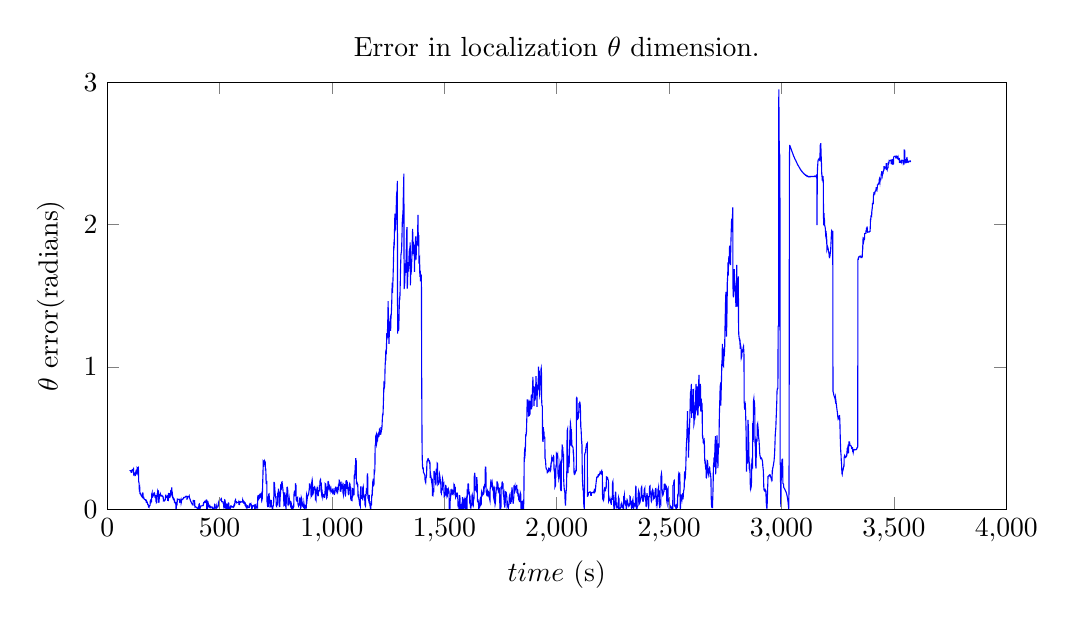
\begin{tikzpicture}

\begin{axis}[
title={Error in localization $\theta$ dimension.},
xlabel={$time$ (s)},
ylabel={$\theta$ error(radians)},
xmin=0, xmax=4000,
ymin=0, ymax=3,
axis on top,
width=13cm,
height=7cm
]
\addplot [blue]
coordinates {
(100,0.269677635251654)
(101,0.2707075624453)
(102,0.270822009445998)
(103,0.270490175279662)
(104,0.268146648145126)
(105,0.267578987347804)
(106,0.268770282211369)
(107,0.258660326366226)
(108,0.259023693427971)
(109,0.259330835501541)
(110,0.259293363590881)
(111,0.276423213845431)
(112,0.276765510902815)
(113,0.277071549202074)
(114,0.275635934501239)
(115,0.279941683269604)
(116,0.280486925124288)
(117,0.2835966355932)
(118,0.248010870482798)
(119,0.251353332056796)
(120,0.250241801841703)
(121,0.251448991566023)
(122,0.241152088742994)
(123,0.239866108869493)
(124,0.235776761782646)
(125,0.236528386830643)
(126,0.256728454496071)
(127,0.260568828557908)
(128,0.265547038291871)
(129,0.25752495345968)
(130,0.25467388844426)
(131,0.249868168964341)
(132,0.248025231490911)
(133,0.279983560516567)
(134,0.274529314417426)
(135,0.26914208550382)
(136,0.287781260019819)
(137,0.293155457402299)
(138,0.294579163586441)
(139,0.281804625187073)
(140,0.197186839973266)
(141,0.187644657727325)
(142,0.183481453382341)
(143,0.134325800531965)
(144,0.136986559931372)
(145,0.14414093084204)
(146,0.110623545923123)
(147,0.110819178268746)
(148,0.106533252852613)
(149,0.105086839673877)
(150,0.0994495512110482)
(151,0.0966735049172915)
(152,0.0938046262621559)
(153,0.0948576723352199)
(154,0.0908212386388543)
(155,0.0873786143940083)
(156,0.0932248614709965)
(157,0.110009801046918)
(158,0.114252774248931)
(159,0.114362779909321)
(160,0.0788516016044205)
(161,0.0781324713210134)
(162,0.0780001041533325)
(163,0.0801036178600853)
(164,0.0717655921389291)
(165,0.0714390583370754)
(166,0.0693921292036099)
(167,0.0668919322847647)
(168,0.0668122953643466)
(169,0.0656482323679517)
(170,0.0637240740611593)
(171,0.0647338479665744)
(172,0.0620512327841818)
(173,0.060901960057564)
(174,0.0482001309348172)
(175,0.0476073523142708)
(176,0.0543804872640936)
(177,0.0496329686768302)
(178,0.049534844924684)
(179,0.0419044447415946)
(180,0.0327613334199739)
(181,0.03313874378265)
(182,0.033077933623233)
(183,0.0286730109891413)
(184,0.0149472297154996)
(185,0.0148104238927793)
(186,0.0127468265323414)
(187,0.0190061101696148)
(188,0.0207340794695059)
(189,0.0249753434285624)
(190,0.0258385512906578)
(191,0.027378100264889)
(192,0.0626148444709948)
(193,0.0639986802547847)
(194,0.0402650740938419)
(195,0.0648482822001761)
(196,0.0509627951854004)
(197,0.0521027927481987)
(198,0.106890546480652)
(199,0.108838364946874)
(200,0.11502558584958)
(201,0.0889163991158002)
(202,0.0851593354132101)
(203,0.0864318933612169)
(204,0.0925341948933891)
(205,0.0989572087976129)
(206,0.0985397251932618)
(207,0.107657888455189)
(208,0.112232086194016)
(209,0.111156082331707)
(210,0.113221197305114)
(211,0.109394898598448)
(212,0.0921344303651255)
(213,0.0828950167099129)
(214,0.083117479416906)
(215,0.0799127779694249)
(216,0.0984401561449299)
(217,0.0609044879119924)
(218,0.0624874328285962)
(219,0.0452588842549737)
(220,0.0470576332954948)
(221,0.0477021965812154)
(222,0.100310351685971)
(223,0.109952223834455)
(224,0.110400860954676)
(225,0.128322736908837)
(226,0.123707781539453)
(227,0.127544933146961)
(228,0.127968572557525)
(229,0.0492171731559134)
(230,0.0478721630548604)
(231,0.0496643543156945)
(232,0.103628145500378)
(233,0.103646675262352)
(234,0.0949137296774474)
(235,0.0956561713737363)
(236,0.0963693892511126)
(237,0.103131869940649)
(238,0.0927135577946101)
(239,0.0922358270695975)
(240,0.0973366388126253)
(241,0.0970353450277672)
(242,0.0965108544462578)
(243,0.0970698879834786)
(244,0.0930093012554491)
(245,0.0929941482189302)
(246,0.0885605238445062)
(247,0.0881285716469815)
(248,0.0893564606246728)
(249,0.0861826562961276)
(250,0.0646848234460169)
(251,0.0679021532088664)
(252,0.0628249320822998)
(253,0.0578981145749597)
(254,0.0569530571538515)
(255,0.058696155505136)
(256,0.0595942609523417)
(257,0.0636723850577283)
(258,0.0657984468818742)
(259,0.0694842503482604)
(260,0.0981584573548784)
(261,0.0978717238490914)
(262,0.0824448073584252)
(263,0.0841084633810871)
(264,0.0854058494451726)
(265,0.0884429132664568)
(266,0.0892622638990972)
(267,0.0905333850319039)
(268,0.0923355887328241)
(269,0.0619104267586312)
(270,0.0615651241293467)
(271,0.0630015646362967)
(272,0.0617989455838046)
(273,0.110539010309084)
(274,0.110896849630263)
(275,0.109640885984968)
(276,0.109506392430101)
(277,0.0822781665572179)
(278,0.0814795070741034)
(279,0.0835980956103917)
(280,0.085568042172369)
(281,0.0971580126668072)
(282,0.104783273728177)
(283,0.130561283294863)
(284,0.131712898472388)
(285,0.124252358161388)
(286,0.126135521138791)
(287,0.152907574906069)
(288,0.114343101251893)
(289,0.120629064510615)
(290,0.111423475483181)
(291,0.0843796185298209)
(292,0.0851429303940694)
(293,0.0760877266433717)
(294,0.0703774604133014)
(295,0.0684259220064454)
(296,0.0751305296974078)
(297,0.072855432225887)
(298,0.0704916869932113)
(299,0.0514128565879646)
(300,0.0522761351956213)
(301,0.0534313611694421)
(302,0.0430792084575917)
(303,0.0434670190612791)
(304,0.0444374024484166)
(305,0.0450472429165645)
(306,0.00372354167523037)
(307,0.00374477923305938)
(308,0.0321014193086866)
(309,0.0318814559718128)
(310,0.0317383450661268)
(311,0.0311047698291076)
(312,0.0693733654301294)
(313,0.0678767137545773)
(314,0.0694045790554636)
(315,0.0692527082686691)
(316,0.0692191077687907)
(317,0.067640910431008)
(318,0.0683033062702765)
(319,0.0678128800542856)
(320,0.0681008469835784)
(321,0.0680274970126087)
(322,0.0686022339930023)
(323,0.0478641791298457)
(324,0.0487976918357451)
(325,0.0508811312887729)
(326,0.0541537978095858)
(327,0.0571031154468118)
(328,0.062905279394851)
(329,0.042917481454777)
(330,0.0500737567476972)
(331,0.0646035416690347)
(332,0.067000564778048)
(333,0.0668246994789769)
(334,0.0670238371882408)
(335,0.0711287271234326)
(336,0.0716894723928711)
(337,0.0726622772386338)
(338,0.0728834461706649)
(339,0.0728576319286824)
(340,0.0817235790036468)
(341,0.0819564241832844)
(342,0.0816208566066654)
(343,0.0813155240587284)
(344,0.0813893460867094)
(345,0.0812669160363131)
(346,0.0811629355734313)
(347,0.084762151803645)
(348,0.0883635214844818)
(349,0.0885839589022199)
(350,0.0903109102171982)
(351,0.0898393742739687)
(352,0.0904650328306788)
(353,0.0902511438741804)
(354,0.0900637618434914)
(355,0.0704514781409964)
(356,0.0707522139990821)
(357,0.0735875681453213)
(358,0.0888018894631068)
(359,0.0886978429464336)
(360,0.0890694559319502)
(361,0.0891231717209389)
(362,0.088156294971917)
(363,0.0878066425034483)
(364,0.0867284585664016)
(365,0.0915389126634507)
(366,0.0822959340014133)
(367,0.0779804891864293)
(368,0.0721290778722119)
(369,0.0688647749084621)
(370,0.0636462787364464)
(371,0.0586680180834829)
(372,0.0541364958987316)
(373,0.0525038949083529)
(374,0.0471233553454835)
(375,0.0425512210838805)
(376,0.0409849526162755)
(377,0.0393581751286447)
(378,0.0360740373612871)
(379,0.0302104906443705)
(380,0.0303714267985942)
(381,0.0296271491504436)
(382,0.0293277969340817)
(383,0.0608306368442275)
(384,0.0608614102212925)
(385,0.0605772547737637)
(386,0.0602515993588542)
(387,0.0592377387699918)
(388,0.0587527523632847)
(389,0.0587288111594493)
(390,0.0147297577707608)
(391,0.0151632414265581)
(392,0.0150966398632699)
(393,0.0166946332239146)
(394,0.0144028184651863)
(395,0.014493991534019)
(396,0.0140001536902294)
(397,0.0112500952414529)
(398,0.0112088873768541)
(399,0.010897402505518)
(400,0.0115140264800901)
(401,0.00569255627293264)
(402,0.00574444368001448)
(403,0.00590508131027456)
(404,0.00593141138858666)
(405,0.00569520815022351)
(406,0.00593779110404968)
(407,0.0063803039398076)
(408,0.0329446438060117)
(409,0.0331078359683823)
(410,0.0348869310609903)
(411,0.00153312094423197)
(412,0.00252264473233765)
(413,0.00401376419689159)
(414,0.00872268583833047)
(415,0.0206816318633614)
(416,0.023168862458192)
(417,0.0232867143366482)
(418,0.022835729860724)
(419,0.0221973860189284)
(420,0.0224593613203126)
(421,0.0226434285997685)
(422,0.0227594321602831)
(423,0.0254009505578572)
(424,0.0253098555248719)
(425,0.0260630235082826)
(426,0.0246681406173193)
(427,0.0251033413851838)
(428,0.0299220221781198)
(429,0.0456639645402566)
(430,0.0455582172718736)
(431,0.0456025053882003)
(432,0.0455915414275911)
(433,0.0549521523433531)
(434,0.0551355352058995)
(435,0.0552945040359483)
(436,0.0551660367968216)
(437,0.0455209447683009)
(438,0.0456067612438642)
(439,0.0457895296186785)
(440,0.063777817260962)
(441,0.0637963419821559)
(442,0.0639789159116384)
(443,0.00392783979539568)
(444,0.00518737068367847)
(445,0.00445947678710534)
(446,0.00278348021772024)
(447,0.0524936827157862)
(448,0.0507477574006707)
(449,0.0492012338843017)
(450,0.0290816323588188)
(451,0.0207687505805529)
(452,0.0177268120270633)
(453,0.0165800121852859)
(454,0.0255765329886133)
(455,0.0262682536997467)
(456,0.0273377390710268)
(457,0.00955605035397156)
(458,0.00873777869145109)
(459,0.00865482891481961)
(460,0.00920402960366151)
(461,0.0158582069950139)
(462,0.01457587912404)
(463,0.0146204366334868)
(464,0.0146146980633162)
(465,0.0152298165786304)
(466,0.0155243877489328)
(467,0.0155435245571069)
(468,0.00525477286904707)
(469,0.00526292519938498)
(470,0.00525468580584776)
(471,0.00440914598462849)
(472,0.00431065032116828)
(473,0.0045986868640171)
(474,0.00544056892040801)
(475,0.00997884688460138)
(476,0.00961906208228447)
(477,0.00859677519956547)
(478,0.0330797139956676)
(479,0.0317604632963353)
(480,0.0309117893786257)
(481,0.00706885625839049)
(482,0.00665599305221787)
(483,0.00764865260741332)
(484,0.00923406406606841)
(485,0.00822260974373723)
(486,0.0107694083438117)
(487,0.0199555759771828)
(488,0.00868633681492237)
(489,0.0110164776250854)
(490,0.0146400217285223)
(491,0.015706009702197)
(492,0.0163105987723211)
(493,0.0167829509901183)
(494,0.022471317622325)
(495,0.0491955467334288)
(496,0.0494034575460644)
(497,0.0496071807356562)
(498,0.0623799301752568)
(499,0.0627810075730699)
(500,0.063315895459823)
(501,0.0636734099644147)
(502,0.0636096212802133)
(503,0.0635534414359629)
(504,0.0635047965625037)
(505,0.0634787618728498)
(506,0.0685676917433187)
(507,0.0745680971414941)
(508,0.0755457688969994)
(509,0.0546610170029249)
(510,0.0513915151228739)
(511,0.0516757623606616)
(512,0.0519956678706372)
(513,0.0523312259479205)
(514,0.0526240198830357)
(515,0.0529175167385496)
(516,0.0415267157667511)
(517,0.0424870937208657)
(518,0.0426240670064719)
(519,0.00843190034440644)
(520,0.00867602392703115)
(521,0.00876168813541511)
(522,0.00887810047613491)
(523,0.064997011723146)
(524,0.0641468353887191)
(525,0.0531092237561332)
(526,0.0191848369876191)
(527,0.0146302130213751)
(528,0.0142839131749775)
(529,3.59611063647236e-05)
(530,0.000666255438740437)
(531,0.00150200921275867)
(532,0.0352998941692306)
(533,0.0347891995325322)
(534,0.0343219030869222)
(535,0.034147684267817)
(536,0.00349944712457506)
(537,0.00325174945387219)
(538,0.0023258268337405)
(539,0.0434082088243557)
(540,0.0431841473823815)
(541,0.0413134848778036)
(542,0.00843531354039939)
(543,0.00158925350281591)
(544,0.00209063199508397)
(545,0.00242476098188837)
(546,0.00126729042628804)
(547,0.00124957955583604)
(548,0.00128434699897562)
(549,0.0221575790494211)
(550,0.022197334190609)
(551,0.0221367855791801)
(552,0.0220501146765628)
(553,0.0160601588820624)
(554,0.0154012735687523)
(555,0.0148351380750811)
(556,0.0141181499488103)
(557,0.0164529864770229)
(558,0.016341726899509)
(559,0.0164955223854655)
(560,0.0160891730839838)
(561,0.0156808140390283)
(562,0.0139785427533039)
(563,0.0225418490612226)
(564,0.0281829437240693)
(565,0.031911220714625)
(566,0.0247681018517678)
(567,0.0277060060489147)
(568,0.0327373742877615)
(569,0.0609614668800946)
(570,0.0625993905249433)
(571,0.0657192303004095)
(572,0.0505397646173462)
(573,0.0508766778950902)
(574,0.0512571928379797)
(575,0.0516310235006749)
(576,0.0445568349327472)
(577,0.0454862846893964)
(578,0.0458174870848114)
(579,0.0463700176187713)
(580,0.0464979007144752)
(581,0.0460675315759904)
(582,0.0465923899380318)
(583,0.0492515094435835)
(584,0.0490605127476915)
(585,0.0524252776628271)
(586,0.033356024382494)
(587,0.0329080361313336)
(588,0.03148524340995)
(589,0.0316550613465769)
(590,0.0528480894015983)
(591,0.0531509270156016)
(592,0.0533871286343954)
(593,0.0473629479096349)
(594,0.0480243724975311)
(595,0.0486142088722559)
(596,0.0497606968282629)
(597,0.0507625665452558)
(598,0.052034416265111)
(599,0.0518713672350162)
(600,0.0517443286366392)
(601,0.0514600605270781)
(602,0.0504452518734233)
(603,0.0650743787827264)
(604,0.0590099612996995)
(605,0.0563536374531415)
(606,0.0518369680268964)
(607,0.0423662426112938)
(608,0.0420213225159856)
(609,0.0517806633641691)
(610,0.0494022636000568)
(611,0.0485929953116968)
(612,0.047483311897329)
(613,0.0300291608788603)
(614,0.0256923741023511)
(615,0.0237054175356473)
(616,0.0352006042299933)
(617,0.0314726383887947)
(618,0.0312656106169489)
(619,0.00922734522927193)
(620,0.00909810947673772)
(621,0.00778150874040917)
(622,0.0229257574662556)
(623,0.0232753971070674)
(624,0.0233685726990647)
(625,0.0237363937628359)
(626,0.011247565843238)
(627,0.0111846935903286)
(628,0.0110896002221834)
(629,0.0118654237179334)
(630,0.0129743292512621)
(631,0.0127273317581278)
(632,0.0122009042737079)
(633,0.030741519573354)
(634,0.0311859223697259)
(635,0.0389728682136061)
(636,0.0383324351614704)
(637,0.0376886573519952)
(638,0.0383099820689043)
(639,0.0396805025686897)
(640,0.022712851207809)
(641,0.0240991455207766)
(642,0.0257783339343485)
(643,0.00432068023134358)
(644,0.00513550814229235)
(645,0.00538154614076203)
(646,0.0165558204866634)
(647,0.0180933282720488)
(648,0.0224079632031711)
(649,0.0210601966247141)
(650,0.0227223745588814)
(651,0.0249862646725629)
(652,0.0244955164437888)
(653,0.025161079286957)
(654,0.0266547048626335)
(655,0.0277293899287463)
(656,0.00394630301324583)
(657,0.00470696817664362)
(658,0.00568215310594478)
(659,0.00660582285145406)
(660,0.0272926376397966)
(661,0.0252937507011945)
(662,0.0285657101287737)
(663,0.0117295649845432)
(664,0.0153673725668706)
(665,0.0101212255652445)
(666,0.0106832256186482)
(667,0.00944132078552484)
(668,0.0105649972542683)
(669,0.00916371818843209)
(670,0.0876498226362237)
(671,0.0933229354639056)
(672,0.0928970581781401)
(673,0.094237653946176)
(674,0.0699717738422125)
(675,0.0721422042692405)
(676,0.0776854958308264)
(677,0.0994737409402395)
(678,0.101011534452486)
(679,0.102935974480792)
(680,0.0828237640371376)
(681,0.0846586391543551)
(682,0.0864648951952045)
(683,0.0888308197723908)
(684,0.0946995518955773)
(685,0.101662619752698)
(686,0.088752511786877)
(687,0.0708050410668217)
(688,0.0797402341005817)
(689,0.0682278476739395)
(690,0.0759322487931968)
(691,0.132864843420339)
(692,0.195440481714559)
(693,0.242676011584354)
(694,0.317557632289481)
(695,0.310218910053027)
(696,0.323489805981171)
(697,0.341544945941303)
(698,0.341649485721599)
(699,0.337849835715261)
(700,0.326388373236119)
(701,0.337552825651079)
(702,0.333553422264385)
(703,0.331056692032762)
(704,0.276090225366271)
(705,0.27697153210361)
(706,0.278266924080818)
(707,0.181212976511993)
(708,0.179856669401597)
(709,0.18759402625907)
(710,0.198473159034694)
(711,0.0531502165165396)
(712,0.0455407420438381)
(713,0.0307035012435766)
(714,0.0357091216635557)
(715,0.0296593014415951)
(716,0.018827076469049)
(717,0.0188756021227061)
(718,0.100890721691641)
(719,0.104753459136801)
(720,0.106550422645042)
(721,0.0881548869971731)
(722,0.0622841521714428)
(723,0.0639525674366006)
(724,0.010390126061494)
(725,0.0223794224754521)
(726,0.0318386743285093)
(727,0.0352063686612702)
(728,0.0541035336780349)
(729,0.0610088844995231)
(730,0.0607575358123924)
(731,0.0213887238176014)
(732,0.0220303570501912)
(733,0.01613360015903)
(734,0.00542212267349806)
(735,0.00354354992641559)
(736,0.00180108594560835)
(737,0.0103225416425445)
(738,0.0232678012393448)
(739,0.0260259802162279)
(740,0.0479110903769984)
(741,0.0498581728397189)
(742,0.188314164754239)
(743,0.188328841586378)
(744,0.183789644696411)
(745,0.161788876083878)
(746,0.132716931919243)
(747,0.126392000871386)
(748,0.0893354401388193)
(749,0.0891966894092109)
(750,0.0802330309348251)
(751,0.0917392661618139)
(752,0.0277327578337934)
(753,0.0216936175534572)
(754,0.0193806036664244)
(755,0.0441460027536307)
(756,0.042410975921892)
(757,0.046652318174109)
(758,0.042848140815058)
(759,0.111455535271564)
(760,0.116696528380164)
(761,0.105413777974793)
(762,0.143516306055137)
(763,0.131023227436925)
(764,0.126742552234317)
(765,0.097787735252167)
(766,0.0191039713854344)
(767,0.0203241750365721)
(768,0.0203286364421986)
(769,0.0764090007423617)
(770,0.0917357406515975)
(771,0.108638438855519)
(772,0.156995875776834)
(773,0.152678575735292)
(774,0.148263390418533)
(775,0.145734330357407)
(776,0.187379677963798)
(777,0.190716639288444)
(778,0.191731385431926)
(779,0.153361651502065)
(780,0.163848206975263)
(781,0.150345131302596)
(782,0.137235620517001)
(783,0.118231354739234)
(784,0.116461111923397)
(785,0.0990183378261127)
(786,0.0396810729679264)
(787,0.0449989881989159)
(788,0.0308878525337335)
(789,0.0335880835717675)
(790,0.116955217148145)
(791,0.0975824206110976)
(792,0.0842542936793278)
(793,0.0237902669359606)
(794,0.0217593557626941)
(795,0.0130312376644293)
(796,0.00200078161319883)
(797,0.0924619876232095)
(798,0.101390824938494)
(799,0.0984180158063055)
(800,0.15225041406818)
(801,0.153544266729765)
(802,0.149003593683236)
(803,0.142180944607258)
(804,0.04137971654806)
(805,0.0443890607663588)
(806,0.0308821332388716)
(807,0.0338449435265793)
(808,0.0513381808731683)
(809,0.0563410118658507)
(810,0.0758082653735981)
(811,0.0628590072778672)
(812,0.0605577265945392)
(813,0.0461183086139278)
(814,0.0342252747569629)
(815,0.0276444027614244)
(816,0.0363713059988269)
(817,0.0565534184635081)
(818,0.0431592462947214)
(819,0.0397540452133576)
(820,0.00527752116378011)
(821,0.01074645556454)
(822,0.00802554031778513)
(823,0.00193799716171039)
(824,0.0176172578775526)
(825,0.014498656715566)
(826,0.00658503929834975)
(827,0.00723886407070462)
(828,0.00733448172806916)
(829,0.0141162109546593)
(830,0.0168756769024065)
(831,0.104914235645263)
(832,0.112776031533509)
(833,0.126768658684819)
(834,0.127275485594078)
(835,0.101365639841638)
(836,0.0957896485062108)
(837,0.0971129326218532)
(838,0.181710966516991)
(839,0.168320431267329)
(840,0.166622109491295)
(841,0.0681219467140142)
(842,0.0691088060328144)
(843,0.060973213467874)
(844,0.063893477846064)
(845,0.0630197591442953)
(846,0.0813785778134455)
(847,0.0827647974077412)
(848,0.0515330333538155)
(849,0.0352157738335232)
(850,0.0281839584214669)
(851,0.0236993342714491)
(852,0.0325029328541937)
(853,0.0292424493545773)
(854,0.0291605678866524)
(855,0.0297827037400191)
(856,0.0337890072282461)
(857,0.0824952414701481)
(858,0.0690795351261992)
(859,0.0673263831273441)
(860,0.00019503979819846)
(861,0.00936791988897156)
(862,0.0149362831270976)
(863,0.0156270214814367)
(864,0.0801378447392211)
(865,0.074837151909402)
(866,0.0693161091712921)
(867,0.0371004741444185)
(868,0.0313649693331368)
(869,0.0347228267855981)
(870,0.0227118903931269)
(871,0.0181472948147547)
(872,0.0160868129350789)
(873,0.0141618549195948)
(874,0.0244213830266133)
(875,0.0430003300491375)
(876,0.0304178937895141)
(877,0.0135204594207845)
(878,0.0170750415509484)
(879,0.0321804496162625)
(880,0.00869838646771082)
(881,0.0100945045294847)
(882,0.0164386343265559)
(883,0.0304516637352652)
(884,0.00748551589826896)
(885,0.00434052917140648)
(886,0.0151550590150349)
(887,0.0999194286272371)
(888,0.0928674984836915)
(889,0.0914565706335102)
(890,0.0756617394949965)
(891,0.0909812625659105)
(892,0.0948378999997874)
(893,0.0958651278448304)
(894,0.0950481756182069)
(895,0.10694182633742)
(896,0.105616484348134)
(897,0.115921534485407)
(898,0.129948431050748)
(899,0.136536686575599)
(900,0.180109882854484)
(901,0.170407159134088)
(902,0.165732737359403)
(903,0.168018979037026)
(904,0.155881928943354)
(905,0.148759191384276)
(906,0.144110442599018)
(907,0.0958687956386406)
(908,0.101537568023972)
(909,0.0984219901678938)
(910,0.186735995341637)
(911,0.196361273447702)
(912,0.206171023069508)
(913,0.195596063851006)
(914,0.109314886847257)
(915,0.104847483464974)
(916,0.109833289997179)
(917,0.137961808865023)
(918,0.141819670836506)
(919,0.135050124274485)
(920,0.152640948789112)
(921,0.154039584210302)
(922,0.148018030559803)
(923,0.144453225068907)
(924,0.151541820138852)
(925,0.145710190818892)
(926,0.131759303050044)
(927,0.0617750607299834)
(928,0.0742365740204707)
(929,0.0678007335270672)
(930,0.126553807211968)
(931,0.131939494786712)
(932,0.134382486846226)
(933,0.141658590348667)
(934,0.122220405573134)
(935,0.113749950388555)
(936,0.123706773119156)
(937,0.105066546387126)
(938,0.0946532491437391)
(939,0.09514586335185)
(940,0.120926495430458)
(941,0.122972935925636)
(942,0.127204332988176)
(943,0.138737376626595)
(944,0.158118890804637)
(945,0.155773903895341)
(946,0.148113124147742)
(947,0.198440253809779)
(948,0.204103194718002)
(949,0.207472835044129)
(950,0.177632940423401)
(951,0.169786730598433)
(952,0.166796185541743)
(953,0.170770757153369)
(954,0.114437689763313)
(955,0.123450770663371)
(956,0.137370328108123)
(957,0.101613994559423)
(958,0.0969913207223152)
(959,0.0852387534683083)
(960,0.0968540191777962)
(961,0.0995717435676235)
(962,0.101021328575253)
(963,0.0949573498790987)
(964,0.0972739109797627)
(965,0.0970688777401403)
(966,0.097804884037173)
(967,0.0786320091687071)
(968,0.105171774183524)
(969,0.106567826919484)
(970,0.177983547343434)
(971,0.175775972661067)
(972,0.176560728054465)
(973,0.162969611111105)
(974,0.154562639821934)
(975,0.150634919384127)
(976,0.078110706391912)
(977,0.0810634544276143)
(978,0.0809320365041399)
(979,0.0972788309044892)
(980,0.117299040698587)
(981,0.126457103253909)
(982,0.195694946919857)
(983,0.186541194332121)
(984,0.192496712062125)
(985,0.190743713149418)
(986,0.149583676259811)
(987,0.153205765749549)
(988,0.155584624230089)
(989,0.145699767223313)
(990,0.139713292424626)
(991,0.152611312870926)
(992,0.144195982005337)
(993,0.143358557218594)
(994,0.143672316732936)
(995,0.131272774094917)
(996,0.140795961858906)
(997,0.130321495288283)
(998,0.122639062920119)
(999,0.12345825708707)
(1000,0.12488028246795)
(1001,0.121831197660758)
(1002,0.117696293624939)
(1003,0.134154928700895)
(1004,0.141930817020133)
(1005,0.141749321637194)
(1006,0.114167479608957)
(1007,0.112668653993685)
(1008,0.120715892086834)
(1009,0.116890301839546)
(1010,0.10315042315834)
(1011,0.10331508148966)
(1012,0.112733336997267)
(1013,0.142054906574329)
(1014,0.14130484997575)
(1015,0.148140607072941)
(1016,0.153123281567327)
(1017,0.154377035586847)
(1018,0.149269787284109)
(1019,0.133950678321096)
(1020,0.14346570668588)
(1021,0.14068187338146)
(1022,0.127722602263768)
(1023,0.124319760693356)
(1024,0.140737220950016)
(1025,0.136034814923117)
(1026,0.126190497432667)
(1027,0.136247996342996)
(1028,0.151108664562622)
(1029,0.169977295090582)
(1030,0.169718889979783)
(1031,0.160539388477142)
(1032,0.203666152253086)
(1033,0.202803746559462)
(1034,0.186685519986591)
(1035,0.176784267826423)
(1036,0.181385485167101)
(1037,0.178603488283981)
(1038,0.181061376149584)
(1039,0.122483911256124)
(1040,0.137148462355672)
(1041,0.154323686034023)
(1042,0.149506311608902)
(1043,0.158011317557453)
(1044,0.161829436269387)
(1045,0.176205006499573)
(1046,0.170492646704557)
(1047,0.152607416222933)
(1048,0.154754375760573)
(1049,0.116143572040497)
(1050,0.108964772791265)
(1051,0.101077021927237)
(1052,0.145311493255265)
(1053,0.170802419833906)
(1054,0.167317665476419)
(1055,0.167162164394229)
(1056,0.154996133689254)
(1057,0.172096376587122)
(1058,0.172230682819146)
(1059,0.101361784332874)
(1060,0.0965802871561374)
(1061,0.100580004689726)
(1062,0.200316791137191)
(1063,0.181536460941168)
(1064,0.183370075601595)
(1065,0.20345927279645)
(1066,0.16884681552851)
(1067,0.175799492110372)
(1068,0.163805407446894)
(1069,0.142966111165556)
(1070,0.158621909241614)
(1071,0.144084172589183)
(1072,0.123530375105739)
(1073,0.104252790366709)
(1074,0.101400942931997)
(1075,0.101890314877147)
(1076,0.147112487390751)
(1077,0.150804206790295)
(1078,0.170948434682455)
(1079,0.179381584809986)
(1080,0.175916007724665)
(1081,0.160696453061733)
(1082,0.149346167443497)
(1083,0.0920319684024282)
(1084,0.0685283519502111)
(1085,0.0646614987577625)
(1086,0.06211463291023)
(1087,0.0627653475657395)
(1088,0.0606361478333477)
(1089,0.0599069578211411)
(1090,0.14578073114265)
(1091,0.144676520522836)
(1092,0.143459225942786)
(1093,0.0953066599866705)
(1094,0.0998458405336695)
(1095,0.100269265701934)
(1096,0.118507262064318)
(1097,0.110983969766895)
(1098,0.108856516853395)
(1099,0.23506266398863)
(1100,0.240039732852439)
(1101,0.215865336903791)
(1102,0.217574155172956)
(1103,0.292857440403354)
(1104,0.288793659518164)
(1105,0.288361607184684)
(1106,0.359286024300432)
(1107,0.33833427996265)
(1108,0.337899834658087)
(1109,0.187445678200685)
(1110,0.190747139660754)
(1111,0.185987570939698)
(1112,0.186534676327948)
(1113,0.169713323562984)
(1114,0.162348176445458)
(1115,0.175399824138377)
(1116,0.0981429751027565)
(1117,0.10150707419998)
(1118,0.100746685173726)
(1119,0.0807118336673733)
(1120,0.0708368732597586)
(1121,0.0593505385335442)
(1122,0.0510170256876323)
(1123,0.029731181419355)
(1124,0.0263255573330432)
(1125,0.0261650211065447)
(1126,0.0207981178424692)
(1127,0.115087814967092)
(1128,0.156921293924507)
(1129,0.156952460096045)
(1130,0.0984387660217982)
(1131,0.0940974522094973)
(1132,0.0761655642011441)
(1133,0.0759637324997773)
(1134,0.075609082290401)
(1135,0.0739145373734284)
(1136,0.0711145048769761)
(1137,0.149675496089702)
(1138,0.152875054491084)
(1139,0.158214498076028)
(1140,0.0803192932649144)
(1141,0.105591196988393)
(1142,0.0995612325637229)
(1143,0.0977046937473678)
(1144,0.0886623720430397)
(1145,0.0695272762689261)
(1146,0.0632407427169197)
(1147,0.0312211509458906)
(1148,0.0249760237370571)
(1149,0.02158964557387)
(1150,0.10587203929387)
(1151,0.090439056637237)
(1152,0.108995552765677)
(1153,0.132316737095365)
(1154,0.128006360153208)
(1155,0.127721783032999)
(1156,0.121961940161554)
(1157,0.231799474067656)
(1158,0.251339195377795)
(1159,0.227369017980663)
(1160,0.0748771616142669)
(1161,0.0843263242397374)
(1162,0.0755261240530676)
(1163,0.0661932315681046)
(1164,0.0746060565117663)
(1165,0.0861714111644691)
(1166,0.100576551817722)
(1167,0.0402529502291149)
(1168,0.0408326996377586)
(1169,0.0279317352807997)
(1170,0.0184713810569523)
(1171,0.0391341656333683)
(1172,0.00895514747862802)
(1173,0.00702929646904482)
(1174,0.0441519500574945)
(1175,0.0413998394626109)
(1176,0.0291742041128604)
(1177,0.0941964011992244)
(1178,0.0961076555660842)
(1179,0.122302605436598)
(1180,0.117634797600512)
(1181,0.186492197929364)
(1182,0.196464634282929)
(1183,0.201360749328923)
(1184,0.21366294777621)
(1185,0.175394995398098)
(1186,0.170340299407746)
(1187,0.175922455533202)
(1188,0.259789571661814)
(1189,0.255062489498945)
(1190,0.266212585733143)
(1191,0.270987652077509)
(1192,0.442930700092746)
(1193,0.452029699682811)
(1194,0.463631422705459)
(1195,0.512333279756663)
(1196,0.51107605854219)
(1197,0.524255663090265)
(1198,0.528475522486981)
(1199,0.463419139219255)
(1200,0.471830166049022)
(1201,0.479202233892956)
(1202,0.480579303606014)
(1203,0.480863911262046)
(1204,0.515502265282572)
(1205,0.522860857800829)
(1206,0.527291347435124)
(1207,0.510926630625937)
(1208,0.512717135198937)
(1209,0.521051132436357)
(1210,0.519235212058402)
(1211,0.5619309636447)
(1212,0.561527583869927)
(1213,0.564287899136673)
(1214,0.526743044143004)
(1215,0.526531502519153)
(1216,0.526984627398642)
(1217,0.527326140945573)
(1218,0.542036194468711)
(1219,0.54127484463351)
(1220,0.569489156222215)
(1221,0.568168200001652)
(1222,0.566362177444849)
(1223,0.595452104677901)
(1224,0.630133126727223)
(1225,0.658855322239565)
(1226,0.667927137280123)
(1227,0.666778516487167)
(1228,0.706094877905263)
(1229,0.757834554560642)
(1230,0.80873283448523)
(1231,0.878818344301771)
(1232,0.873316698218923)
(1233,0.853257245936592)
(1234,0.859547558289723)
(1235,0.890172918698055)
(1236,0.975616702336692)
(1237,1.02288590796968)
(1238,1.04652044104428)
(1239,1.08667774577739)
(1240,1.07841902808114)
(1241,1.12244627923215)
(1242,1.0923357861209)
(1243,1.17867228689923)
(1244,1.23679491415505)
(1245,1.20139673214883)
(1246,1.20887207245078)
(1247,1.24595582054186)
(1248,1.30505972383162)
(1249,1.36717686073698)
(1250,1.46341416796901)
(1251,1.21677522702841)
(1252,1.20916152639773)
(1253,1.25964252545026)
(1254,1.16297145082143)
(1255,1.23904730328245)
(1256,1.28976063564121)
(1257,1.28176840573947)
(1258,1.28076455161206)
(1259,1.31602603562429)
(1260,1.36039773110451)
(1261,1.25282779625818)
(1262,1.31286357297736)
(1263,1.37538991691773)
(1264,1.36521971881366)
(1265,1.41268049738414)
(1266,1.45269993298596)
(1267,1.52952571564263)
(1268,1.59184299601908)
(1269,1.55905246316707)
(1270,1.55130859027695)
(1271,1.5868549481457)
(1272,1.63970938607713)
(1273,1.69699433156177)
(1274,1.77046535638049)
(1275,1.84472080645143)
(1276,1.87125132744192)
(1277,1.86493241739825)
(1278,1.9407246024061)
(1279,2.00319399919312)
(1280,2.07855354740606)
(1281,2.02700228393153)
(1282,1.99009439542906)
(1283,1.98233906158477)
(1284,2.0151102436227)
(1285,2.04362944843554)
(1286,2.11827737631453)
(1287,2.1943073530841)
(1288,2.2165232086309)
(1289,2.21102398926147)
(1290,2.247846889741)
(1291,2.30735681399285)
(1292,1.23491027026951)
(1293,1.29464751222409)
(1294,1.35886610675194)
(1295,1.37054954566677)
(1296,1.25229646524208)
(1297,1.2652973345303)
(1298,1.32234359148974)
(1299,1.40138430509801)
(1300,1.45859704900617)
(1301,1.49571485433812)
(1302,1.47374567005868)
(1303,1.52967036925608)
(1304,1.59858440349198)
(1305,1.68060428759997)
(1306,1.74005685959603)
(1307,1.79093224915472)
(1308,1.79996507866329)
(1309,1.81174564667916)
(1310,1.83101663160218)
(1311,1.88886932077898)
(1312,1.95061790953715)
(1313,2.02398473457864)
(1314,2.04540751749149)
(1315,2.03802906867528)
(1316,2.07523989130287)
(1317,2.16405092954184)
(1318,2.22868399351384)
(1319,2.2996189047247)
(1320,2.35858601076899)
(1321,1.54666976841537)
(1322,1.56109005643175)
(1323,1.57935450845766)
(1324,1.59273821346417)
(1325,1.6616867954379)
(1326,1.72818139563023)
(1327,1.67635722916593)
(1328,1.66077456865131)
(1329,1.69680641063333)
(1330,1.78394087620855)
(1331,1.84094830074191)
(1332,1.91755660840154)
(1333,1.9660648464489)
(1334,1.9834608550438)
(1335,1.55014735813893)
(1336,1.57774074568825)
(1337,1.63686813332273)
(1338,1.6832760426754)
(1339,1.73682935987963)
(1340,1.71297246786294)
(1341,1.67042349725133)
(1342,1.71786056448128)
(1343,1.78236894931415)
(1344,1.81540836384351)
(1345,1.82653392122798)
(1346,1.83181659092997)
(1347,1.82708944247906)
(1348,1.87565940181163)
(1349,1.57335911630054)
(1350,1.66333282943924)
(1351,1.75440723111027)
(1352,1.64849178066885)
(1353,1.68363264652111)
(1354,1.69874154006793)
(1355,1.75248305102541)
(1356,1.78889058133318)
(1357,1.86261081724118)
(1358,1.93398016842228)
(1359,1.97062270220552)
(1360,1.85187563829307)
(1361,1.83710531339198)
(1362,1.87942811668068)
(1363,1.79364352401376)
(1364,1.85783096144008)
(1365,1.85162281311204)
(1366,1.83573800019076)
(1367,1.66826616852631)
(1368,1.73939627288928)
(1369,1.80552974968304)
(1370,1.81595104812732)
(1371,1.87011417999019)
(1372,1.90809413670649)
(1373,1.91688504939783)
(1374,1.75458958592676)
(1375,1.7958691424507)
(1376,1.88426885440534)
(1377,1.85920193843613)
(1378,1.86133975890534)
(1379,1.84990906325238)
(1380,1.88962165438756)
(1381,1.93307020519242)
(1382,2.00435902927384)
(1383,2.06925313084984)
(1384,1.88300866892134)
(1385,1.91183218432163)
(1386,1.91424481881664)
(1387,1.72683336893654)
(1388,1.74553289061285)
(1389,1.75643241683682)
(1390,1.76210104360413)
(1391,1.63326292757625)
(1392,1.678898490003)
(1393,1.66887680979652)
(1394,1.60142368186777)
(1395,1.62616047693514)
(1396,1.63334513514527)
(1397,1.6358547134032)
(1398,1.63899135387483)
(1399,0.995022035337025)
(1400,0.684092364235401)
(1401,0.416567944165909)
(1402,0.337064422823684)
(1403,0.299881127942868)
(1404,0.286647636770928)
(1405,0.28709312800843)
(1406,0.28810719598583)
(1407,0.25973038018377)
(1408,0.259270988582356)
(1409,0.253704335161002)
(1410,0.249795960304525)
(1411,0.246242466763515)
(1412,0.243461046426574)
(1413,0.239608662945855)
(1414,0.206825585445016)
(1415,0.198077897630743)
(1416,0.190855630561249)
(1417,0.18640354221715)
(1418,0.216889646314629)
(1419,0.219554593184341)
(1420,0.22971313010077)
(1421,0.243556947003311)
(1422,0.302823592464632)
(1423,0.337040324823949)
(1424,0.337580022064987)
(1425,0.33979182042837)
(1426,0.347128233615854)
(1427,0.35449604410888)
(1428,0.355088361635067)
(1429,0.349272691435962)
(1430,0.343458967162876)
(1431,0.340586177911784)
(1432,0.341060071577877)
(1433,0.330821463232487)
(1434,0.325337418237564)
(1435,0.331256113638291)
(1436,0.326725064387046)
(1437,0.220376430304358)
(1438,0.2298771280332)
(1439,0.242569096643041)
(1440,0.230612925269467)
(1441,0.225458434936303)
(1442,0.207621165669787)
(1443,0.19758688467457)
(1444,0.219036446665444)
(1445,0.203325887923159)
(1446,0.204111039347557)
(1447,0.0969726762617173)
(1448,0.0964766705160478)
(1449,0.0947562342991759)
(1450,0.103968767020431)
(1451,0.139446022962818)
(1452,0.138373846299685)
(1453,0.135142554716173)
(1454,0.266396608782873)
(1455,0.256553133611752)
(1456,0.26015920585974)
(1457,0.255415532094957)
(1458,0.224732539631514)
(1459,0.229055627729832)
(1460,0.232750241725626)
(1461,0.178287804789761)
(1462,0.174633196985269)
(1463,0.183773660677898)
(1464,0.261974043789733)
(1465,0.256838008263423)
(1466,0.260790397555455)
(1467,0.250483921572715)
(1468,0.323649471637641)
(1469,0.321686918160726)
(1470,0.318367109976948)
(1471,0.170653548900277)
(1472,0.172872822014809)
(1473,0.179751205905742)
(1474,0.175347407064802)
(1475,0.176738956659502)
(1476,0.18578142644412)
(1477,0.199674305222398)
(1478,0.201703892504266)
(1479,0.239570632991782)
(1480,0.231181447809032)
(1481,0.220395255317381)
(1482,0.201351258154428)
(1483,0.190250327992654)
(1484,0.190217233226686)
(1485,0.12045791415596)
(1486,0.121615724369004)
(1487,0.113746430455759)
(1488,0.127216460845485)
(1489,0.143101948044315)
(1490,0.145502720617226)
(1491,0.143317023765369)
(1492,0.213117111813277)
(1493,0.206055262930692)
(1494,0.187839541760277)
(1495,0.175580993936401)
(1496,0.164428236720884)
(1497,0.165302110213273)
(1498,0.170922883057017)
(1499,0.0845871182070299)
(1500,0.0813731949767389)
(1501,0.0841616524641555)
(1502,0.110284268846565)
(1503,0.108818947615818)
(1504,0.104967769269105)
(1505,0.0949634536332828)
(1506,0.164865897953509)
(1507,0.163859134332028)
(1508,0.154132481456485)
(1509,0.134206709943808)
(1510,0.141130190970961)
(1511,0.141920891618496)
(1512,0.0867521820712165)
(1513,0.0897625031497453)
(1514,0.110711663947918)
(1515,0.11171446913901)
(1516,0.127744437698598)
(1517,0.123028006524727)
(1518,0.109055618086039)
(1519,0.133255977124921)
(1520,0.126356536399288)
(1521,0.121645597617789)
(1522,0.0058813466290637)
(1523,0.00445590055895462)
(1524,0.00280556190516901)
(1525,0.00533024888701128)
(1526,0.0571269953897482)
(1527,0.0727762600681072)
(1528,0.0798222737635838)
(1529,0.123476225781985)
(1530,0.119368173752118)
(1531,0.127397158129974)
(1532,0.131247923354163)
(1533,0.119772543513776)
(1534,0.113648252751002)
(1535,0.120742810079475)
(1536,0.107865676840083)
(1537,0.109718669240162)
(1538,0.107142680824533)
(1539,0.128519366995231)
(1540,0.126756609451756)
(1541,0.125607072875634)
(1542,0.120283712201551)
(1543,0.169694074929491)
(1544,0.165045948733375)
(1545,0.166957340353899)
(1546,0.158869295509482)
(1547,0.131011474638925)
(1548,0.134057712735355)
(1549,0.137810280159504)
(1550,0.0820435952250069)
(1551,0.0858557406667775)
(1552,0.103871329932468)
(1553,0.107538667330854)
(1554,0.11001418785887)
(1555,0.107540825523599)
(1556,0.0863273457065008)
(1557,0.104514281861462)
(1558,0.107085023479959)
(1559,0.0844053380702228)
(1560,0.0870326572608739)
(1561,0.0210458156612505)
(1562,0.0227732057771588)
(1563,0.0461259535602236)
(1564,0.0223410599953437)
(1565,0.00285395111743192)
(1566,0.0171340049043653)
(1567,0.0247623799870773)
(1568,0.0976701650513796)
(1569,0.0871783705617028)
(1570,0.0651353915473329)
(1571,0.00625631048012787)
(1572,0.00322860011268578)
(1573,0.00590927617062054)
(1574,0.00876192697968836)
(1575,0.00120562458697204)
(1576,0.0230096723354185)
(1577,0.0301472776168001)
(1578,0.00485746801678477)
(1579,0.0118005579852589)
(1580,0.00219699230486903)
(1581,0.0845834425391274)
(1582,0.071172029829202)
(1583,0.0723149767172915)
(1584,0.0645995783096884)
(1585,0.000351396197337372)
(1586,0.0113165702613776)
(1587,0.0153802235549252)
(1588,0.0607333064588791)
(1589,0.0645746438486703)
(1590,0.0691960490987804)
(1591,0.0132692673108439)
(1592,0.0103698321565133)
(1593,0.00180886405065106)
(1594,0.013056552260692)
(1595,0.0790416596493477)
(1596,0.064802319956406)
(1597,0.0660158517952172)
(1598,0.0730499691749955)
(1599,0.00864018140836009)
(1600,0.0133239364762758)
(1601,0.00690106391782308)
(1602,0.123510770794738)
(1603,0.119423517983358)
(1604,0.115644037499634)
(1605,0.179034622430316)
(1606,0.168417624241675)
(1607,0.181391058440647)
(1608,0.152321157524069)
(1609,0.114204987663482)
(1610,0.115983493638863)
(1611,0.116684948990694)
(1612,0.102513211169783)
(1613,0.0540218672128954)
(1614,0.0587913425331448)
(1615,0.0657605014795863)
(1616,0.00901248034961011)
(1617,0.0184379476564298)
(1618,0.00786903584594123)
(1619,0.0209308489247619)
(1620,0.027595645411095)
(1621,0.0364644403320087)
(1622,0.0360615555955301)
(1623,0.0836554940549239)
(1624,0.0777842125614687)
(1625,0.0869271478375002)
(1626,0.0481067096927328)
(1627,0.0571575703835356)
(1628,0.0473331528520453)
(1629,0.0390635140976179)
(1630,0.0802930843821037)
(1631,0.0695761967472501)
(1632,0.0766653335081777)
(1633,0.227359216172521)
(1634,0.237783551073076)
(1635,0.251398951788135)
(1636,0.2511335182478)
(1637,0.140662263567495)
(1638,0.142754477629325)
(1639,0.146369911910853)
(1640,0.132497456255048)
(1641,0.130226750024274)
(1642,0.135402447906831)
(1643,0.130105934468606)
(1644,0.224825960015455)
(1645,0.20746876894454)
(1646,0.194629338650662)
(1647,0.0617240275380428)
(1648,0.0520590049338754)
(1649,0.0521407287444564)
(1650,0.0676898650701734)
(1651,0.0478550019936312)
(1652,0.0352757825778474)
(1653,0.00388235890135657)
(1654,0.00681293418460083)
(1655,0.0265692494606275)
(1656,0.0331382228789527)
(1657,0.0076133775321443)
(1658,0.047626461371002)
(1659,0.0665495962585707)
(1660,0.0729172992269893)
(1661,0.0658289407129784)
(1662,0.0279499683507245)
(1663,0.029748843143464)
(1664,0.0337384714524194)
(1665,0.11034535056315)
(1666,0.122720766797285)
(1667,0.116150451132476)
(1668,0.105147765451773)
(1669,0.100776723554088)
(1670,0.110320797042841)
(1671,0.112280988901435)
(1672,0.104502809881176)
(1673,0.103585274014224)
(1674,0.114380748314479)
(1675,0.159743753192729)
(1676,0.146129233919739)
(1677,0.136923426975204)
(1678,0.160731902558996)
(1679,0.17046592079912)
(1680,0.169000295436649)
(1681,0.16606364141096)
(1682,0.276339686688675)
(1683,0.295685266357554)
(1684,0.295546133255061)
(1685,0.27058538634446)
(1686,0.115870802226705)
(1687,0.12443239523886)
(1688,0.12535026846776)
(1689,0.0948771281366052)
(1690,0.0941789080068309)
(1691,0.112718055458351)
(1692,0.124758471237107)
(1693,0.116844160159196)
(1694,0.116789844869023)
(1695,0.106776313906854)
(1696,0.125092579102462)
(1697,0.125437221773288)
(1698,0.106041663609764)
(1699,0.105926845033215)
(1700,0.0992095000694091)
(1701,0.0912235300640161)
(1702,0.0664031315247113)
(1703,0.0588906198392207)
(1704,0.142228972362649)
(1705,0.161309793787372)
(1706,0.160939301450359)
(1707,0.208233722959272)
(1708,0.193293927128382)
(1709,0.177266706782943)
(1710,0.168411515475642)
(1711,0.173784531824935)
(1712,0.173535983366605)
(1713,0.181694180993076)
(1714,0.147855182983915)
(1715,0.139942053991108)
(1716,0.14373750856429)
(1717,0.155463773735917)
(1718,0.150872271647067)
(1719,0.0831076296335933)
(1720,0.0758387095720661)
(1721,0.144559768060251)
(1722,0.148520555348909)
(1723,0.128246616003967)
(1724,0.0578433080282261)
(1725,0.0615614036269685)
(1726,0.0334064879490077)
(1727,0.0413008984141894)
(1728,0.0776452626091641)
(1729,0.103502700659832)
(1730,0.115212891395451)
(1731,0.156027050179104)
(1732,0.142284917642309)
(1733,0.132890875289428)
(1734,0.194562996717356)
(1735,0.174764881998687)
(1736,0.172762277296532)
(1737,0.182906244104117)
(1738,0.178769396028674)
(1739,0.167250423318472)
(1740,0.141208190867069)
(1741,0.149571549632047)
(1742,0.146020470375475)
(1743,0.132049092489365)
(1744,0.111432805646402)
(1745,0.132522504008703)
(1746,0.136706628068678)
(1747,0.00617976225443906)
(1748,0.00289663094398263)
(1749,0.00442079343928725)
(1750,0.00199020094039914)
(1751,0.00810868012520549)
(1752,0.0162932922505243)
(1753,0.153804846535374)
(1754,0.154220684144523)
(1755,0.138684986778988)
(1756,0.179512306331363)
(1757,0.189452581955746)
(1758,0.190047650907641)
(1759,0.166498404090676)
(1760,0.16328348072739)
(1761,0.167083808558168)
(1762,0.107954908231053)
(1763,0.0988902017200539)
(1764,0.108460862733465)
(1765,0.114456025773862)
(1766,0.036791635092738)
(1767,0.0342009475982583)
(1768,0.0283802272786326)
(1769,0.0117489425173485)
(1770,0.0324548788055403)
(1771,0.0486567939613476)
(1772,0.118678510535648)
(1773,0.116963305995728)
(1774,0.119766595790283)
(1775,0.118123065261714)
(1776,0.112951874657361)
(1777,0.0883595917782496)
(1778,0.0888100858371454)
(1779,0.0257496256906289)
(1780,0.0341777252765096)
(1781,0.0392511730921186)
(1782,0.0189631564915444)
(1783,0.0173143428815914)
(1784,0.014600572043137)
(1785,0.00905606750647658)
(1786,0.027260288180369)
(1787,0.032070511070597)
(1788,0.0347687476813374)
(1789,0.0838248969022603)
(1790,0.0956241926921457)
(1791,0.10020532446035)
(1792,0.0764122869046577)
(1793,0.0721314187523059)
(1794,0.0605300144653849)
(1795,0.0373224784981541)
(1796,0.0555415487486788)
(1797,0.0632580326508649)
(1798,0.0516383930679329)
(1799,0.119623026637655)
(1800,0.127340185748708)
(1801,0.152852197470438)
(1802,0.134278604122173)
(1803,0.0701636311731453)
(1804,0.0686365441086853)
(1805,0.0714298436085845)
(1806,0.0365672927017475)
(1807,0.056794948470142)
(1808,0.062847913768437)
(1809,0.0867376062686707)
(1810,0.167477689277675)
(1811,0.152052151564803)
(1812,0.155754712935832)
(1813,0.160189358577427)
(1814,0.165478442389813)
(1815,0.132680178214159)
(1816,0.138724220045205)
(1817,0.140894797690507)
(1818,0.145753818624016)
(1819,0.151147590078708)
(1820,0.147905594729182)
(1821,0.151279403422322)
(1822,0.171175435710993)
(1823,0.116443225242492)
(1824,0.114212367976379)
(1825,0.116718114646446)
(1826,0.141862582471766)
(1827,0.123029949199952)
(1828,0.090766774546899)
(1829,0.0879658766189442)
(1830,0.0872168542682976)
(1831,0.0633491335302443)
(1832,0.079645941206798)
(1833,0.0667850786685795)
(1834,0.0492997564706803)
(1835,0.0763386247999791)
(1836,0.0627719293717708)
(1837,0.0592721579034294)
(1838,0.11501431420781)
(1839,0.109861661702025)
(1840,0.103980248815942)
(1841,0.00489836556501411)
(1842,0.00343425988815449)
(1843,0.00696221977915368)
(1844,0.00604078685018283)
(1845,0.0281790443611429)
(1846,0.0201552524146722)
(1847,0.0215290229450078)
(1848,0.0594262770908838)
(1849,0.0272901497875075)
(1850,0.00429469087167789)
(1851,0.0110203579161983)
(1852,0.000761674265125745)
(1853,0.0347638674874511)
(1854,0.102551639687604)
(1855,0.315160778027362)
(1856,0.38422854654907)
(1857,0.404134709764707)
(1858,0.393776048351515)
(1859,0.385599754196096)
(1860,0.4121247021523)
(1861,0.447251757052231)
(1862,0.525716235306549)
(1863,0.511570257511425)
(1864,0.541363482740212)
(1865,0.525567823466349)
(1866,0.587263639857433)
(1867,0.64466735704746)
(1868,0.722372010191343)
(1869,0.771197426905296)
(1870,0.719665710928525)
(1871,0.7302100492725)
(1872,0.744937219851635)
(1873,0.755507113606654)
(1874,0.650186674864016)
(1875,0.722445467681609)
(1876,0.769939156443797)
(1877,0.670232055903397)
(1878,0.654188608945332)
(1879,0.70315662232133)
(1880,0.76056628404922)
(1881,0.665310971920828)
(1882,0.718754718390087)
(1883,0.748324466618544)
(1884,0.731195387014766)
(1885,0.745623396341845)
(1886,0.757515472169831)
(1887,0.804859814043954)
(1888,0.701423999663308)
(1889,0.743255388014567)
(1890,0.716848297067535)
(1891,0.79496570958252)
(1892,0.840471687749577)
(1893,0.873748345918502)
(1894,0.929378094525797)
(1895,0.819411764715619)
(1896,0.84982922946855)
(1897,0.852592274576483)
(1898,0.835673661899244)
(1899,0.725272881805579)
(1900,0.775594486862103)
(1901,0.849206029444615)
(1902,0.860438852694386)
(1903,0.808200496372336)
(1904,0.787222632625218)
(1905,0.782564223701558)
(1906,0.833303782153897)
(1907,0.887311417844416)
(1908,0.93474783114778)
(1909,0.869307871686724)
(1910,0.868662370412054)
(1911,0.863624688463256)
(1912,0.718912573490234)
(1913,0.795293568139366)
(1914,0.847334085469535)
(1915,0.870006047626427)
(1916,0.873274103244236)
(1917,0.866141167906514)
(1918,0.919623662115697)
(1919,1.002120804371)
(1920,0.914583752748144)
(1921,0.952076176489218)
(1922,0.972990185609352)
(1923,0.814354275788955)
(1924,0.801122222700906)
(1925,0.815558068768797)
(1926,0.877511438296852)
(1927,0.876836017088709)
(1928,0.939457372145472)
(1929,0.924393892602739)
(1930,0.98378123746973)
(1931,0.991563192883251)
(1932,0.96182576362516)
(1933,0.771192950948525)
(1934,0.727280620600894)
(1935,0.727010448758937)
(1936,0.72459091871953)
(1937,0.507957536821644)
(1938,0.481994740092996)
(1939,0.472961855278543)
(1940,0.575692353401403)
(1941,0.562386664838268)
(1942,0.547817047605688)
(1943,0.545289323119179)
(1944,0.505748147927965)
(1945,0.509065761364106)
(1946,0.507477573862753)
(1947,0.50230902071157)
(1948,0.35628264109197)
(1949,0.352641010795615)
(1950,0.344088513525948)
(1951,0.321300036235713)
(1952,0.294640391166498)
(1953,0.288653004916648)
(1954,0.280813579971219)
(1955,0.280317820894856)
(1956,0.277456209721266)
(1957,0.274156414497671)
(1958,0.257419491272846)
(1959,0.259782096069506)
(1960,0.262133748396756)
(1961,0.262883094769311)
(1962,0.262274267477489)
(1963,0.264212378955358)
(1964,0.286050785784358)
(1965,0.288585160179759)
(1966,0.286854262393926)
(1967,0.285106012493648)
(1968,0.273469459143969)
(1969,0.274430136055862)
(1970,0.273779467298233)
(1971,0.266600075136525)
(1972,0.269609798167355)
(1973,0.280671807813594)
(1974,0.322255804079721)
(1975,0.311932601842234)
(1976,0.334447131368468)
(1977,0.338062565649996)
(1978,0.362858339321936)
(1979,0.3576232875857)
(1980,0.346857506769069)
(1981,0.353287705244412)
(1982,0.354592237866395)
(1983,0.349956817247663)
(1984,0.359206903742393)
(1985,0.364131311902543)
(1986,0.371964549580534)
(1987,0.367960758442004)
(1988,0.280513590846362)
(1989,0.269707027067737)
(1990,0.272420448983456)
(1991,0.255069437600085)
(1992,0.158577036358677)
(1993,0.163792652237955)
(1994,0.161544939890878)
(1995,0.165152810274457)
(1996,0.30537294342797)
(1997,0.288531084802558)
(1998,0.30562527513508)
(1999,0.390794083250215)
(2000,0.38756493735825)
(2001,0.384313999382482)
(2002,0.373447391843126)
(2003,0.379256684422331)
(2004,0.384295113990614)
(2005,0.355082838997501)
(2006,0.229146208045466)
(2007,0.241899526109179)
(2008,0.235923340335038)
(2009,0.215669014966786)
(2010,0.225628869043728)
(2011,0.229480061348592)
(2012,0.246934510435973)
(2013,0.30069892692293)
(2014,0.298467461100471)
(2015,0.327862324273836)
(2016,0.318316848097992)
(2017,0.142997273884911)
(2018,0.145576681651372)
(2019,0.139972542701448)
(2020,0.126204867618017)
(2021,0.330511775104187)
(2022,0.345308554595195)
(2023,0.346325078866303)
(2024,0.455350110194504)
(2025,0.43036689598006)
(2026,0.422607861812085)
(2027,0.435403420942694)
(2028,0.389135976674825)
(2029,0.376124288308293)
(2030,0.387846631350786)
(2031,0.207210226218462)
(2032,0.172306033085346)
(2033,0.150500655408263)
(2034,0.134672576795578)
(2035,0.127523431788445)
(2036,0.116796000163317)
(2037,0.0712771883711816)
(2038,0.0422199631587268)
(2039,0.0251089518412351)
(2040,0.0675425303622483)
(2041,0.109653642353863)
(2042,0.126857089992037)
(2043,0.141825026016694)
(2044,0.196647623885884)
(2045,0.281824777234807)
(2046,0.504482807923569)
(2047,0.554940866638436)
(2048,0.560907359101339)
(2049,0.269140059926077)
(2050,0.254189195666271)
(2051,0.293966422412353)
(2052,0.349213703159052)
(2053,0.357275872114855)
(2054,0.307080569300609)
(2055,0.295006424743491)
(2056,0.356478384319502)
(2057,0.42129682618733)
(2058,0.475866044495063)
(2059,0.548367011089261)
(2060,0.571733261187012)
(2061,0.606886272778419)
(2062,0.598323113215755)
(2063,0.446716785981452)
(2064,0.489908155604397)
(2065,0.562241200908219)
(2066,0.51829266230682)
(2067,0.463811249091422)
(2068,0.442511052443778)
(2069,0.441916697452442)
(2070,0.441733620927452)
(2071,0.438288430549918)
(2072,0.434452856990291)
(2073,0.430491573742373)
(2074,0.379128044388223)
(2075,0.398632753100144)
(2076,0.329890387579926)
(2077,0.258295867635193)
(2078,0.247938560318352)
(2079,0.248962514098884)
(2080,0.245404262614541)
(2081,0.248001491969926)
(2082,0.253328588038186)
(2083,0.265461511239572)
(2084,0.266393578026712)
(2085,0.272360767118901)
(2086,0.275940405085951)
(2087,0.274207953244716)
(2088,0.77860711270225)
(2089,0.783451807189081)
(2090,0.781070250521694)
(2091,0.634521992708283)
(2092,0.681195828866844)
(2093,0.626224132447908)
(2094,0.667118219346067)
(2095,0.665572701602531)
(2096,0.636570547021732)
(2097,0.656983392930224)
(2098,0.679167286656418)
(2099,0.744531264111374)
(2100,0.720400180276155)
(2101,0.745203733766018)
(2102,0.748935440901146)
(2103,0.736204511138604)
(2104,0.751020316542247)
(2105,0.710687580879792)
(2106,0.676195497752435)
(2107,0.577124788776355)
(2108,0.568105582057877)
(2109,0.539416988431287)
(2110,0.499542056916925)
(2111,0.458570876887999)
(2112,0.47839618637128)
(2113,0.343001659492)
(2114,0.216729627314206)
(2115,0.185142148670223)
(2116,0.160114769593606)
(2117,0.136372344120345)
(2118,0.136329274649698)
(2119,0.107916193035597)
(2120,0.0455729287948046)
(2121,0.0191716107549968)
(2122,0.0107186409510041)
(2123,0.00409074706058243)
(2124,0.37231755349641)
(2125,0.390700375684048)
(2126,0.394488640553597)
(2127,0.397078804707422)
(2128,0.397589706014272)
(2129,0.416493709052737)
(2130,0.430735164458505)
(2131,0.441785452261194)
(2132,0.451054141639127)
(2133,0.456726674771358)
(2134,0.455329622499267)
(2135,0.456945391672839)
(2136,0.46040083930911)
(2137,0.091329997008073)
(2138,0.09211817026998)
(2139,0.0941343018503238)
(2140,0.100270004003946)
(2141,0.110904235219583)
(2142,0.114364634945742)
(2143,0.116538822369624)
(2144,0.117399466434849)
(2145,0.118133202910332)
(2146,0.118515436661431)
(2147,0.120735011536716)
(2148,0.120329443074735)
(2149,0.120285612047414)
(2150,0.120355619387162)
(2151,0.0985161778258283)
(2152,0.0984716018213145)
(2153,0.0968916957947043)
(2154,0.096965766104276)
(2155,0.115756209170201)
(2156,0.115759106730984)
(2157,0.115940382740135)
(2158,0.117757083066815)
(2159,0.117492866369707)
(2160,0.117700456951171)
(2161,0.117856559551329)
(2162,0.118077646663107)
(2163,0.115369937490247)
(2164,0.115553056230344)
(2165,0.123946941216051)
(2166,0.124693850948379)
(2167,0.130715586097687)
(2168,0.143955066165898)
(2169,0.118963000545289)
(2170,0.121051390137534)
(2171,0.123529264119513)
(2172,0.138177395214386)
(2173,0.145096227408446)
(2174,0.173299679414428)
(2175,0.18180102377484)
(2176,0.199171847437862)
(2177,0.211055189254783)
(2178,0.222295423947673)
(2179,0.221748918505784)
(2180,0.227622226557162)
(2181,0.227875276756998)
(2182,0.229908998459335)
(2183,0.228772873902495)
(2184,0.236123288893873)
(2185,0.233618960470042)
(2186,0.242488282235376)
(2187,0.243563211976402)
(2188,0.244829635589235)
(2189,0.243071518360488)
(2190,0.246534403871824)
(2191,0.242376752875963)
(2192,0.244363464277149)
(2193,0.257475563424719)
(2194,0.254324764345852)
(2195,0.253662121388384)
(2196,0.256764291459018)
(2197,0.260406665694398)
(2198,0.255807168506515)
(2199,0.266407582633627)
(2200,0.269793656865603)
(2201,0.260164388666397)
(2202,0.258738293200369)
(2203,0.25972501538192)
(2204,0.0714333795383322)
(2205,0.0701953430368185)
(2206,0.0705872533134095)
(2207,0.0641898703405097)
(2208,0.0717629833699025)
(2209,0.0693061859129984)
(2210,0.0791245054856548)
(2211,0.129133514400427)
(2212,0.139602746452461)
(2213,0.14520853444714)
(2214,0.140394191475426)
(2215,0.132357219290332)
(2216,0.129748219590592)
(2217,0.132235476203568)
(2218,0.148244635023232)
(2219,0.14605214508143)
(2220,0.148190120542567)
(2221,0.227083347628362)
(2222,0.226584971205315)
(2223,0.225473602443145)
(2224,0.218855298490443)
(2225,0.223246774235296)
(2226,0.221921918959106)
(2227,0.214684511288057)
(2228,0.208488669072854)
(2229,0.204448801137183)
(2230,0.198500051029053)
(2231,0.0564647365437723)
(2232,0.0610385259689665)
(2233,0.061002500196123)
(2234,0.0607045385615521)
(2235,0.0605680124212804)
(2236,0.0613023329196256)
(2237,0.0727166074929517)
(2238,0.064020306493628)
(2239,0.0646437144695016)
(2240,0.0449012605234151)
(2241,0.0435552324033495)
(2242,0.0453031096385912)
(2243,0.0295859649417327)
(2244,0.0743132280987413)
(2245,0.0751041485735766)
(2246,0.069775371843805)
(2247,0.0697484047290193)
(2248,0.176988457276868)
(2249,0.190043061202994)
(2250,0.195140372658751)
(2251,0.0966626424688512)
(2252,0.0911606001272909)
(2253,0.0922879649276842)
(2254,0.0104624448944586)
(2255,0.0011743725982698)
(2256,0.00457410204784736)
(2257,0.00251393562649627)
(2258,0.0366030477046086)
(2259,0.0397070025981905)
(2260,0.0374686766999437)
(2261,0.118813312029793)
(2262,0.118899710331488)
(2263,0.114188129982861)
(2264,0.034508430340821)
(2265,0.0245360376295154)
(2266,0.0361108327305293)
(2267,0.0384914334531783)
(2268,0.0152837248323561)
(2269,0.0143476226638564)
(2270,0.012888832791409)
(2271,0.0152397029995193)
(2272,0.0111674778410924)
(2273,0.00754729154261691)
(2274,0.0157290006029478)
(2275,0.0821830420870353)
(2276,0.0762582184563829)
(2277,0.0738270700878512)
(2278,0.00546306390988827)
(2279,0.000498764023900033)
(2280,0.00169623241862071)
(2281,6.99030362025787e-05)
(2282,0.00381474103956902)
(2283,0.00543837605328434)
(2284,0.00733130617374034)
(2285,0.0129070493367318)
(2286,0.0318796590786174)
(2287,0.0369137813542846)
(2288,0.0160052755815054)
(2289,0.0160018839710387)
(2290,0.0161277706900602)
(2291,0.0317205451709324)
(2292,0.012156504700064)
(2293,0.0112296347205429)
(2294,0.0214310310617787)
(2295,0.00613492892631973)
(2296,0.00225319507673616)
(2297,7.59661906712949e-06)
(2298,0.0815762393451362)
(2299,0.0797778005964473)
(2300,0.0883713744367478)
(2301,0.097685370671063)
(2302,0.049943495691664)
(2303,0.0443923973114262)
(2304,0.0387910298448113)
(2305,0.047430617089566)
(2306,0.0512891884542705)
(2307,0.0550329120903452)
(2308,0.0531228290944536)
(2309,0.00453403443281886)
(2310,0.00571864973937508)
(2311,0.00754696668775168)
(2312,0.0575588976251473)
(2313,0.0664992124992003)
(2314,0.0632633971734484)
(2315,0.0597949031340277)
(2316,0.0451909644372215)
(2317,0.0407174131170422)
(2318,0.0334795143690489)
(2319,0.0246949808907293)
(2320,0.0293910604205512)
(2321,0.0264220086349787)
(2322,0.0239837511335286)
(2323,0.0230256012988423)
(2324,0.0261155717422401)
(2325,0.0377085581966292)
(2326,0.0888215294678614)
(2327,0.086607557080026)
(2328,0.0621768429118519)
(2329,0.0609851292413501)
(2330,0.0321646308768146)
(2331,0.0438653182843396)
(2332,0.0579609869653055)
(2333,7.10097604184057e-06)
(2334,0.0064479769496355)
(2335,0.0105739555853472)
(2336,0.017911615176518)
(2337,0.0532861302137184)
(2338,0.0622109763777074)
(2339,0.067958229633382)
(2340,0.0149575811273963)
(2341,0.0127671481291265)
(2342,0.00530504601672277)
(2343,0.014446060849437)
(2344,0.0223605557414825)
(2345,0.037979863580865)
(2346,0.0360683530541643)
(2347,0.0289418329093087)
(2348,0.0216363929797598)
(2349,0.0220652192828008)
(2350,0.0284425942842215)
(2351,0.151426564613678)
(2352,0.159090366857447)
(2353,0.15714967711957)
(2354,0.0096894973728352)
(2355,0.000720113589352422)
(2356,0.00612172290783519)
(2357,0.00148039303820724)
(2358,0.017950450122667)
(2359,0.0176236608733507)
(2360,0.0223483734265613)
(2361,0.0239024666531891)
(2362,0.101488682787607)
(2363,0.114100383885014)
(2364,0.124735261533805)
(2365,0.113068195745744)
(2366,0.118663678004265)
(2367,0.112298063873384)
(2368,0.0388144739576841)
(2369,0.0415077584040264)
(2370,0.0471460004292226)
(2371,0.0489675115497952)
(2372,0.0657192824430188)
(2373,0.0698347092363534)
(2374,0.0796401347951701)
(2375,0.0805812961917369)
(2376,0.145186658871828)
(2377,0.153417799544988)
(2378,0.157118423643821)
(2379,0.102379899440787)
(2380,0.0911613091326271)
(2381,0.0844504589646076)
(2382,0.0599711188143184)
(2383,0.0566779149873522)
(2384,0.0551938408143173)
(2385,0.056637540177165)
(2386,0.0921919803544826)
(2387,0.0915892845609885)
(2388,0.0909520347325774)
(2389,0.134355779413732)
(2390,0.14155085166231)
(2391,0.142508931125107)
(2392,0.147187561171957)
(2393,0.0769689724112057)
(2394,0.070011008836528)
(2395,0.0806940782976149)
(2396,0.0738961010400949)
(2397,0.0215704600021986)
(2398,0.0200472720787181)
(2399,0.0247131279556183)
(2400,0.0953403382246782)
(2401,0.0988055695368022)
(2402,0.112421504321115)
(2403,0.0860288669161209)
(2404,0.0882465097575662)
(2405,0.0823691324259381)
(2406,0.0770615555378557)
(2407,0.0247830734750338)
(2408,0.0152887146453882)
(2409,0.00981936374057124)
(2410,0.0879615760949126)
(2411,0.0899093058794857)
(2412,0.0892976193525032)
(2413,0.152455036947458)
(2414,0.161414220416873)
(2415,0.163053324854491)
(2416,0.115381705109409)
(2417,0.105111604963699)
(2418,0.104752668105483)
(2419,0.106378320357437)
(2420,0.0592642946738477)
(2421,0.0540584494240459)
(2422,0.0608270839112834)
(2423,0.118892973596762)
(2424,0.115729686015728)
(2425,0.117011365708393)
(2426,0.123242731092734)
(2427,0.135322997881472)
(2428,0.130868213935236)
(2429,0.125610746770946)
(2430,0.0789798110274948)
(2431,0.0840317117180467)
(2432,0.0755832191952366)
(2433,0.0776296021003282)
(2434,0.0767912776993489)
(2435,0.0843500904500076)
(2436,0.0854182972765178)
(2437,0.117483805565861)
(2438,0.122215897851826)
(2439,0.138693146788114)
(2440,0.14445717804304)
(2441,0.145267386694004)
(2442,0.137310707491534)
(2443,0.048341725502806)
(2444,0.0547463048349308)
(2445,0.0413344867379868)
(2446,0.0277061547936404)
(2447,0.0413930687905752)
(2448,0.0422427262497598)
(2449,0.0329572380838448)
(2450,0.139234157217806)
(2451,0.140866324219349)
(2452,0.144234843677951)
(2453,0.153517588167562)
(2454,0.117319699549779)
(2455,0.112467601602628)
(2456,0.11592884145585)
(2457,0.0256482546022267)
(2458,0.0147141494592757)
(2459,0.00543921585564178)
(2460,0.0583526473994986)
(2461,0.063554604122384)
(2462,0.06276239814839)
(2463,0.0552620434821271)
(2464,0.23154728940359)
(2465,0.240271676880211)
(2466,0.249632726040573)
(2467,0.232988518535639)
(2468,0.141236923204008)
(2469,0.135066372173548)
(2470,0.132281808068625)
(2471,0.105782211043792)
(2472,0.0970640121642212)
(2473,0.100920523252309)
(2474,0.106806705906958)
(2475,0.116682084491662)
(2476,0.123292848216555)
(2477,0.124767338256537)
(2478,0.17258915556885)
(2479,0.174525537018773)
(2480,0.172557411671725)
(2481,0.166315940181415)
(2482,0.179253265946414)
(2483,0.1538902909681)
(2484,0.135550917856098)
(2485,0.161081934495532)
(2486,0.163692368575075)
(2487,0.160120835442731)
(2488,0.159333990510722)
(2489,0.0716005883356478)
(2490,0.0520863812111778)
(2491,0.0444236786747592)
(2492,0.119512336928421)
(2493,0.129209223713831)
(2494,0.138910882245697)
(2495,0.143281775309025)
(2496,0.0532209840424938)
(2497,0.066420716546685)
(2498,0.058904152211011)
(2499,0.0549611470999425)
(2500,0.0196557994202138)
(2501,0.0271948601978584)
(2502,0.0195771124547766)
(2503,0.0281212827985158)
(2504,0.0189368338736866)
(2505,0.0162216700094913)
(2506,0.0206246669816945)
(2507,0.0182060474011276)
(2508,0.0035593425460454)
(2509,0.00342996785411032)
(2510,0.00694584685097999)
(2511,0.00988925482797986)
(2512,0.00605307807774835)
(2513,0.00285592422139569)
(2514,0.0117619625992225)
(2515,0.00147417576528053)
(2516,0.000231571636065908)
(2517,0.166718638205034)
(2518,0.168585453118262)
(2519,0.168854106830218)
(2520,0.172714664179694)
(2521,0.190032724801314)
(2522,0.201460054487067)
(2523,0.20269199029364)
(2524,0.0238174389610921)
(2525,0.0221164055369805)
(2526,0.0200542943899689)
(2527,0.029204071958528)
(2528,0.0276557275155644)
(2529,0.0274542209488318)
(2530,0.00724057406956247)
(2531,0.000437073332016258)
(2532,0.00516553680481646)
(2533,0.00900754436462714)
(2534,0.0298922451521553)
(2535,0.0281754812178923)
(2536,0.0232499972372153)
(2537,0.0199720323982886)
(2538,0.10374002443695)
(2539,0.0905271817865594)
(2540,0.0988427554033646)
(2541,0.113024599102036)
(2542,0.239622087430184)
(2543,0.247921493638492)
(2544,0.239682880964315)
(2545,0.231966073974464)
(2546,0.243668500072973)
(2547,0.246774943122723)
(2548,0.228705172087465)
(2549,0.00727209957538033)
(2550,0.00556902157784167)
(2551,0.0134682478925892)
(2552,0.0989836785038607)
(2553,0.0997020781678453)
(2554,0.0960950706113865)
(2555,0.0754752997440864)
(2556,0.0755793118646597)
(2557,0.06561181788387)
(2558,0.0812460940061208)
(2559,0.0946806041097683)
(2560,0.10427465462468)
(2561,0.102770063502274)
(2562,0.0686048265263435)
(2563,0.0953173962364544)
(2564,0.120411643291582)
(2565,0.132241061595289)
(2566,0.137565352869331)
(2567,0.1485828167042)
(2568,0.217946567043509)
(2569,0.266154021537027)
(2570,0.242296437792687)
(2571,0.213671720884207)
(2572,0.219887802813403)
(2573,0.251110354874484)
(2574,0.285756131502515)
(2575,0.346607062884628)
(2576,0.414471665759473)
(2577,0.464110208649288)
(2578,0.480252808061035)
(2579,0.507382566897872)
(2580,0.578150851025157)
(2581,0.628373169644647)
(2582,0.688538310708033)
(2583,0.549153929267065)
(2584,0.550199453758993)
(2585,0.57049926704749)
(2586,0.362507788477339)
(2587,0.409095528173447)
(2588,0.45989444941366)
(2589,0.513880082369688)
(2590,0.551475060135964)
(2591,0.575730779171827)
(2592,0.635619795792175)
(2593,0.69195046460962)
(2594,0.764440102002158)
(2595,0.817868628672768)
(2596,0.826298961866904)
(2597,0.834582108523953)
(2598,0.850256460620367)
(2599,0.881281424092028)
(2600,0.641698006318781)
(2601,0.708275665763921)
(2602,0.704022070888646)
(2603,0.677019870787861)
(2604,0.703728823031206)
(2605,0.773606501137165)
(2606,0.844631630207768)
(2607,0.779218294687625)
(2608,0.826522214111794)
(2609,0.830930065825567)
(2610,0.592949606793368)
(2611,0.600442293571813)
(2612,0.643788825402988)
(2613,0.712633779690307)
(2614,0.729901986614507)
(2615,0.674024345771116)
(2616,0.665345573036589)
(2617,0.716044020278684)
(2618,0.784106826091197)
(2619,0.856141013745788)
(2620,0.881023322242225)
(2621,0.696607712207481)
(2622,0.708943169356811)
(2623,0.701969824257702)
(2624,0.737407065132997)
(2625,0.806656918988649)
(2626,0.862672291711665)
(2627,0.670876207341801)
(2628,0.657200702717987)
(2629,0.691013657932988)
(2630,0.745674399467075)
(2631,0.850390922547358)
(2632,0.909734514862376)
(2633,0.944319134987815)
(2634,0.752724642253473)
(2635,0.722118017929556)
(2636,0.744881625533448)
(2637,0.791182831854439)
(2638,0.849873437473359)
(2639,0.88077061051165)
(2640,0.839950323163702)
(2641,0.686324709706072)
(2642,0.737633100444314)
(2643,0.7767524594713)
(2644,0.73214611399339)
(2645,0.746317275298476)
(2646,0.744052345143313)
(2647,0.72529087845241)
(2648,0.52681897135102)
(2649,0.506658348456256)
(2650,0.508322346262906)
(2651,0.49374882304228)
(2652,0.46853185806978)
(2653,0.469203377909451)
(2654,0.464798535442023)
(2655,0.477450495943767)
(2656,0.482909421590354)
(2657,0.467152604400956)
(2658,0.350224291511266)
(2659,0.335026075406732)
(2660,0.33981738686076)
(2661,0.330197447719785)
(2662,0.298263597111019)
(2663,0.301914152498158)
(2664,0.300730845816234)
(2665,0.221940606699592)
(2666,0.220721503586775)
(2667,0.235386650665232)
(2668,0.250305805011222)
(2669,0.342487773859024)
(2670,0.341193211492576)
(2671,0.335686677470973)
(2672,0.318813749924472)
(2673,0.259250462619059)
(2674,0.256893904377613)
(2675,0.249323307965789)
(2676,0.279827023623445)
(2677,0.282776510110059)
(2678,0.282738687521421)
(2679,0.277800813368165)
(2680,0.292529876751427)
(2681,0.290261268778988)
(2682,0.256319545372673)
(2683,0.226142482416686)
(2684,0.255028947772439)
(2685,0.230899486275371)
(2686,0.224661843141243)
(2687,0.102229953668505)
(2688,0.0485721600711315)
(2689,0.0196047665263812)
(2690,0.0214486178188871)
(2691,0.0186571756090323)
(2692,0.0166367848796511)
(2693,0.00680559541607906)
(2694,0.0728566687884431)
(2695,0.122368295151244)
(2696,0.186321042451336)
(2697,0.311074443134739)
(2698,0.291913253206388)
(2699,0.336835844437492)
(2700,0.364237462046336)
(2701,0.296257249924839)
(2702,0.350814596112324)
(2703,0.379402171512828)
(2704,0.455715445143115)
(2705,0.462679512290759)
(2706,0.513499397276444)
(2707,0.244598566977782)
(2708,0.28182153338905)
(2709,0.292835155043639)
(2710,0.38082051790122)
(2711,0.407584072784083)
(2712,0.479967186267173)
(2713,0.518536638312697)
(2714,0.408999510350263)
(2715,0.391049878761709)
(2716,0.369772947811523)
(2717,0.287922895455814)
(2718,0.356277723151905)
(2719,0.44151548264431)
(2720,0.461319899471767)
(2721,0.447214007555093)
(2722,0.432916850259541)
(2723,0.61491637452329)
(2724,0.686471438490198)
(2725,0.744855607646801)
(2726,0.785969249395494)
(2727,0.861662637370723)
(2728,0.87139535821014)
(2729,0.861804613126184)
(2730,0.727236742428149)
(2731,0.79479999316761)
(2732,0.856455170762983)
(2733,0.90821842378449)
(2734,1.01963763587981)
(2735,1.01123151721089)
(2736,1.08058733285993)
(2737,1.16170935125678)
(2738,1.0600558526451)
(2739,1.12031263928956)
(2740,1.13763808716184)
(2741,1.00827078405863)
(2742,1.00501870621091)
(2743,1.04885711405522)
(2744,1.12509122375494)
(2745,1.07480154071099)
(2746,1.10587216425783)
(2747,1.11269566614876)
(2748,1.22547109250675)
(2749,1.30118111346613)
(2750,1.37637180091858)
(2751,1.45120760153554)
(2752,1.5055107074561)
(2753,1.52408902819775)
(2754,1.52407885039227)
(2755,1.21345788309352)
(2756,1.2641550479146)
(2757,1.3588358787509)
(2758,1.42257377781592)
(2759,1.62614468974029)
(2760,1.60497619700586)
(2761,1.66218373907866)
(2762,1.73477951558882)
(2763,1.64293901743942)
(2764,1.71035650670017)
(2765,1.75555179938163)
(2766,1.77845005119791)
(2767,1.75489049742077)
(2768,1.76411962079261)
(2769,1.85289905585785)
(2770,1.72717699697865)
(2771,1.79937145403279)
(2772,1.75615914455308)
(2773,1.71566601014389)
(2774,1.81090540355696)
(2775,1.87949156090139)
(2776,1.93937214910506)
(2777,1.99050913452624)
(2778,2.03484311773895)
(2779,2.03872871333255)
(2780,2.03771645253978)
(2781,2.04143589902191)
(2782,2.06363323805939)
(2783,2.12134831501257)
(2784,1.57569270869803)
(2785,1.50942736407827)
(2786,1.48899995824408)
(2787,1.56600185027432)
(2788,1.57238640179943)
(2789,1.63690836271357)
(2790,1.68808232536625)
(2791,1.53245171075772)
(2792,1.5466716532604)
(2793,1.56106703179043)
(2794,1.55363691933539)
(2795,1.4908481534579)
(2796,1.50328638181176)
(2797,1.42265064790931)
(2798,1.60400212146427)
(2799,1.60534566766668)
(2800,1.65309938914228)
(2801,1.71757542467762)
(2802,1.42342588058758)
(2803,1.51043946208466)
(2804,1.54057393508065)
(2805,1.55408402910489)
(2806,1.56147973473018)
(2807,1.58352017263716)
(2808,1.63740588213152)
(2809,1.27235765616244)
(2810,1.22734404588884)
(2811,1.21311059455222)
(2812,1.20035965415484)
(2813,1.19166991441345)
(2814,1.19380216301253)
(2815,1.19418444133082)
(2816,1.12767947393188)
(2817,1.14483269418308)
(2818,1.15171137969866)
(2819,1.14220813128084)
(2820,1.13097183675871)
(2821,1.0625085109882)
(2822,1.06836832856042)
(2823,1.07386633214376)
(2824,1.1015227494838)
(2825,1.12268651482484)
(2826,1.10119720567784)
(2827,1.119552967976)
(2828,1.12308465237652)
(2829,1.12232617436598)
(2830,1.13841968550037)
(2831,1.14411806369821)
(2832,1.11932653802137)
(2833,1.08727003502349)
(2834,0.756116653407615)
(2835,0.729145769576233)
(2836,0.700192576820654)
(2837,0.720614074344438)
(2838,0.719983922980417)
(2839,0.729155900619615)
(2840,0.701078706152429)
(2841,0.632796873069991)
(2842,0.572921686537255)
(2843,0.501907332805877)
(2844,0.26350569116043)
(2845,0.335347840060462)
(2846,0.415580956183444)
(2847,0.332082746468555)
(2848,0.328496354550193)
(2849,0.326912025546079)
(2850,0.334545406613843)
(2851,0.627676929448144)
(2852,0.58933107099344)
(2853,0.544851316595692)
(2854,0.473164673543807)
(2855,0.377275945988001)
(2856,0.312591286130686)
(2857,0.272478662819451)
(2858,0.316374309749192)
(2859,0.307699888994188)
(2860,0.259413104553909)
(2861,0.178743070993969)
(2862,0.146829582718897)
(2863,0.154221872767199)
(2864,0.171951083663594)
(2865,0.158292627342139)
(2866,0.16643512193868)
(2867,0.234507778991522)
(2868,0.338185573328795)
(2869,0.349975476930383)
(2870,0.347006110600816)
(2871,0.285684376524063)
(2872,0.604196458623978)
(2873,0.520144066586445)
(2874,0.473564946188944)
(2875,0.751796486797436)
(2876,0.766118464498741)
(2877,0.776966626241911)
(2878,0.749604683786738)
(2879,0.76317925699811)
(2880,0.739839132311236)
(2881,0.708760704536935)
(2882,0.471873364829331)
(2883,0.447423188366378)
(2884,0.434648895216284)
(2885,0.313629966838499)
(2886,0.297758705139539)
(2887,0.286044227059138)
(2888,0.480945143513218)
(2889,0.478535827863864)
(2890,0.477012573617605)
(2891,0.478822318812918)
(2892,0.591886606932786)
(2893,0.596265028536812)
(2894,0.601530983556029)
(2895,0.581404233011621)
(2896,0.571221413997865)
(2897,0.534232053295623)
(2898,0.509805983082313)
(2899,0.49456333446472)
(2900,0.484085102724728)
(2901,0.456850296957886)
(2902,0.430270888090698)
(2903,0.393302075050825)
(2904,0.379494970466226)
(2905,0.370872546888256)
(2906,0.364440484637857)
(2907,0.358262536344867)
(2908,0.354297929067726)
(2909,0.355287933972409)
(2910,0.354672187474765)
(2911,0.358645086051817)
(2912,0.35636242575806)
(2913,0.351061375350238)
(2914,0.344956769352176)
(2915,0.337905732011301)
(2916,0.327105539762258)
(2917,0.298976693916601)
(2918,0.287915215648072)
(2919,0.272590380756399)
(2920,0.236893904727492)
(2921,0.160761775641815)
(2922,0.136327420488679)
(2923,0.134887883910785)
(2924,0.131432196601925)
(2925,0.134661938940702)
(2926,0.126994361883541)
(2927,0.125410683335604)
(2928,0.134047649502336)
(2929,0.130571953848704)
(2930,0.126910963119804)
(2931,0.101932012500106)
(2932,0.0496934438365093)
(2933,0.027279405830563)
(2934,0.0144750418077906)
(2935,0.00387509241064388)
(2936,0.0205635856619062)
(2937,0.0750997084906282)
(2938,0.137354840852715)
(2939,0.175165948786236)
(2940,0.22934600663677)
(2941,0.230494177056896)
(2942,0.23398745796921)
(2943,0.23450428800464)
(2944,0.235202739539485)
(2945,0.23616532803093)
(2946,0.240228792175963)
(2947,0.238555389861439)
(2948,0.235356489213492)
(2949,0.240270755838019)
(2950,0.240036225679783)
(2951,0.227378738700394)
(2952,0.227004894880855)
(2953,0.223913344366519)
(2954,0.218279726156665)
(2955,0.208070441152738)
(2956,0.214170161442954)
(2957,0.218533261305276)
(2958,0.214225949476275)
(2959,0.270194240967034)
(2960,0.270067258320781)
(2961,0.289573938218972)
(2962,0.293625110343219)
(2963,0.302270265970324)
(2964,0.307674485799682)
(2965,0.321393270920398)
(2966,0.330129081416408)
(2967,0.341199579788324)
(2968,0.362385809100971)
(2969,0.382418358377919)
(2970,0.418944174103245)
(2971,0.462363833240971)
(2972,0.515353282592997)
(2973,0.541254326380596)
(2974,0.555039394326314)
(2975,0.582400576822266)
(2976,0.631417387775883)
(2977,0.666071576677069)
(2978,0.714778968743786)
(2979,0.756609907053217)
(2980,0.82872964968513)
(2981,0.83879311816375)
(2982,0.849104543827281)
(2983,0.849104543827281)
(2984,0.849104543827281)
(2985,1.28683005800079)
(2986,1.28683005800079)
(2987,1.28683005800079)
(2988,2.95098865995575)
(2989,2.74566873381306)
(2990,2.52865758011509)
(2991,2.49556956658532)
(2992,2.49244379982744)
(2993,2.29500852510725)
(2994,0.335387904585154)
(2995,0.296525195629151)
(2996,0.152179927022011)
(2997,0.0162691775865866)
(2998,0.144911780565231)
(2999,0.238012082486598)
(3000,0.277298356949537)
(3001,0.318492475508897)
(3002,0.346581151320784)
(3003,0.349925833366065)
(3004,0.351904596512391)
(3005,0.351881041820157)
(3006,0.180738778578396)
(3007,0.179794564636703)
(3008,0.177891277850884)
(3009,0.1758562875011)
(3010,0.15244313960265)
(3011,0.150730317320449)
(3012,0.147264738196282)
(3013,0.144803652634619)
(3014,0.141617015098928)
(3015,0.138759383328034)
(3016,0.134547567788286)
(3017,0.130017721887453)
(3018,0.127927939502297)
(3019,0.124530744833646)
(3020,0.120913199942334)
(3021,0.116814852088464)
(3022,0.112082300569637)
(3023,0.105484960462673)
(3024,0.0997488441427778)
(3025,0.0912346242477726)
(3026,0.0839714206305873)
(3027,0.0736768379358183)
(3028,0.0616067884040605)
(3029,0.0504058984590303)
(3030,0.037257735945059)
(3031,0.0152679526729118)
(3032,0.00669675567023642)
(3033,0.0616895357596148)
(3034,0.491560419417692)
(3035,2.3480618238568)
(3036,2.55748549998996)
(3037,2.55744902820831)
(3038,2.5539274749676)
(3039,2.54918816949746)
(3040,2.54349316827527)
(3041,2.53957447766831)
(3042,2.53563012167385)
(3043,2.53076721712521)
(3044,2.52671209521165)
(3045,2.52172896902582)
(3046,2.51798048018052)
(3047,2.51292778745799)
(3048,2.50931775647721)
(3049,2.50458790672517)
(3050,2.50101975056848)
(3051,2.4957185092712)
(3052,2.49157490938476)
(3053,2.48702404120511)
(3054,2.48251977594143)
(3055,2.47958852521649)
(3056,2.4767572342748)
(3057,2.4728257109741)
(3058,2.46867873411199)
(3059,2.46447704949921)
(3060,2.46171735118648)
(3061,2.4574582575219)
(3062,2.45483634163199)
(3063,2.4537793353297)
(3064,2.44851118904578)
(3065,2.44556845651048)
(3066,2.44139041119295)
(3067,2.43853953360619)
(3068,2.43508011750916)
(3069,2.43233055035623)
(3070,2.42819573097902)
(3071,2.42458232278975)
(3072,2.42186922739299)
(3073,2.41867321865673)
(3074,2.41680032511747)
(3075,2.41473223998716)
(3076,2.41193674535996)
(3077,2.40829834722488)
(3078,2.40614651198073)
(3079,2.40336790246463)
(3080,2.40109854711725)
(3081,2.39881770995951)
(3082,2.39627954395062)
(3083,2.39169490554875)
(3084,2.3891445822878)
(3085,2.38724534791934)
(3086,2.38597829112357)
(3087,2.38138689877039)
(3088,2.38058857196981)
(3089,2.37755465992766)
(3090,2.37584724017458)
(3091,2.37627679673412)
(3092,2.37318952782468)
(3093,2.36961124074103)
(3094,2.36836512147372)
(3095,2.36701499012222)
(3096,2.3652508365262)
(3097,2.36234525118877)
(3098,2.36049802292061)
(3099,2.35963755903456)
(3100,2.35985841594036)
(3101,2.35642804220649)
(3102,2.35385745685878)
(3103,2.35380815241249)
(3104,2.35365078341735)
(3105,2.35138953290468)
(3106,2.34893106459228)
(3107,2.35059931093881)
(3108,2.3501927180873)
(3109,2.34589242457466)
(3110,2.34465711179243)
(3111,2.34565265639273)
(3112,2.34373248461222)
(3113,2.34421674883513)
(3114,2.34028792730121)
(3115,2.34219188941231)
(3116,2.34064454026109)
(3117,2.33981109247131)
(3118,2.33966385453411)
(3119,2.33919917701448)
(3120,2.33838531592798)
(3121,2.33640233156209)
(3122,2.33809894483008)
(3123,2.33885809822411)
(3124,2.33763156571829)
(3125,2.33664345051099)
(3126,2.33782945884329)
(3127,2.33850621300687)
(3128,2.33744245263685)
(3129,2.3374296199722)
(3130,2.33941800763884)
(3131,2.33919715073305)
(3132,2.33818066860428)
(3133,2.33820768474059)
(3134,2.33917216076904)
(3135,2.33896616273657)
(3136,2.33787673709546)
(3137,2.33817729159589)
(3138,2.33953012459776)
(3139,2.33988268516939)
(3140,2.33822592063322)
(3141,2.33818066860792)
(3142,2.33963278583494)
(3143,2.33901073930563)
(3144,2.33832858189951)
(3145,2.33806652539304)
(3146,2.33778893460064)
(3147,2.33820700929161)
(3148,2.34131656638008)
(3149,2.33987458019644)
(3150,2.33827860203698)
(3151,2.34033588079862)
(3152,2.34050675785645)
(3153,2.34228914744697)
(3154,2.34330157715838)
(3155,2.34687783814977)
(3156,2.34860957240696)
(3157,2.33487321821983)
(3158,1.99754028407867)
(3159,2.27555437000458)
(3160,2.39556668708489)
(3161,2.41556403050587)
(3162,2.44268417740628)
(3163,2.45452197278306)
(3164,2.45606130150069)
(3165,2.45946795165461)
(3166,2.46188918825161)
(3167,2.46280444428945)
(3168,2.46746126624445)
(3169,2.46702976790645)
(3170,2.4532007992772)
(3171,2.45139890744273)
(3172,2.55999482299443)
(3173,2.56016299843099)
(3174,2.56096470226543)
(3175,2.57328866637299)
(3176,2.4901616854623)
(3177,2.46979935952478)
(3178,2.41905369319822)
(3179,2.35535073865882)
(3180,2.34975108572842)
(3181,2.31472047671574)
(3182,2.31472047671574)
(3183,2.31472047671574)
(3184,2.30891403389993)
(3185,2.34071143550697)
(3186,2.29064775092426)
(3187,2.04615162037074)
(3188,1.99456414805682)
(3189,2.0815512889141)
(3190,2.04583552721813)
(3191,2.03600366462412)
(3192,1.9987839065364)
(3193,1.98776869219884)
(3194,1.9842119982366)
(3195,1.97264754370508)
(3196,1.94488119739932)
(3197,1.91894387897853)
(3198,1.91385129800667)
(3199,1.90383466895867)
(3200,1.91767620836767)
(3201,1.90012141636172)
(3202,1.8279288234459)
(3203,1.8345375025224)
(3204,1.85112257888506)
(3205,1.84620918230179)
(3206,1.83957537020582)
(3207,1.83349804849389)
(3208,1.82701894584137)
(3209,1.80887902090818)
(3210,1.80637998627991)
(3211,1.8065080460467)
(3212,1.78280074384274)
(3213,1.76808054819879)
(3214,1.7684553788944)
(3215,1.77738826367695)
(3216,1.78659484058566)
(3217,1.79918102834242)
(3218,1.8101961776948)
(3219,1.82986932772756)
(3220,1.8675609320736)
(3221,1.89380913380147)
(3222,1.93691405433775)
(3223,1.95399559627832)
(3224,1.94963118005392)
(3225,1.94909142360619)
(3226,1.9544028892562)
(3227,1.95441802604582)
(3228,1.9534264342647)
(3229,0.829092314606848)
(3230,0.823278556976484)
(3231,0.819442732925534)
(3232,0.807641646933354)
(3233,0.802397397219756)
(3234,0.794536377176263)
(3235,0.792468292045959)
(3236,0.78685628097839)
(3237,0.782253491565206)
(3238,0.779430980899923)
(3239,0.769411709805112)
(3240,0.785537598768831)
(3241,0.774647394309402)
(3242,0.764635214696288)
(3243,0.749199503215611)
(3244,0.737760195622802)
(3245,0.720800183827639)
(3246,0.710763732085586)
(3247,0.697088797690928)
(3248,0.686876698511303)
(3249,0.672567602361202)
(3250,0.65545351442194)
(3251,0.643437454591155)
(3252,0.633475887703359)
(3253,0.636409206895739)
(3254,0.644228351882309)
(3255,0.651426801106543)
(3256,0.650392083099693)
(3257,0.656172860527993)
(3258,0.657092802166123)
(3259,0.639274226441164)
(3260,0.59466784255125)
(3261,0.529373979135532)
(3262,0.46883081824996)
(3263,0.426162885441561)
(3264,0.395551599501748)
(3265,0.37765877129056)
(3266,0.339531594826956)
(3267,0.321965027540107)
(3268,0.279961671619792)
(3269,0.25097605952539)
(3270,0.245217570043285)
(3271,0.260355385891278)
(3272,0.265963935698498)
(3273,0.270766750383307)
(3274,0.276168626672704)
(3275,0.286110543585498)
(3276,0.294592956020613)
(3277,0.302044660258223)
(3278,0.302268706234615)
(3279,0.366223238264938)
(3280,0.369592825738509)
(3281,0.377248523147573)
(3282,0.373841113034432)
(3283,0.367314014673029)
(3284,0.36683447828007)
(3285,0.363022501640517)
(3286,0.364438822553057)
(3287,0.368823904307479)
(3288,0.369851461051372)
(3289,0.372415402707253)
(3290,0.3826362018435)
(3291,0.38118877956985)
(3292,0.425102222947486)
(3293,0.424460447264163)
(3294,0.424498924150566)
(3295,0.434619130354771)
(3296,0.427933005118629)
(3297,0.396437866510979)
(3298,0.396607232404507)
(3299,0.445571995233784)
(3300,0.471514503741691)
(3301,0.471334171038524)
(3302,0.472961872140349)
(3303,0.472847074671353)
(3304,0.447350569500629)
(3305,0.447682150343241)
(3306,0.447240478732199)
(3307,0.447199258020334)
(3308,0.445550619506464)
(3309,0.445510002351575)
(3310,0.444149223418418)
(3311,0.442501677244639)
(3312,0.426603684282046)
(3313,0.426963674275786)
(3314,0.426562295580742)
(3315,0.432712294695941)
(3316,0.432455870994794)
(3317,0.406266231835726)
(3318,0.406419292681782)
(3319,0.397925880119251)
(3320,0.406945805867203)
(3321,0.417519929269487)
(3322,0.41899829302086)
(3323,0.419117094318063)
(3324,0.41905797233207)
(3325,0.419040123524862)
(3326,0.418848280220913)
(3327,0.417326088944537)
(3328,0.418845493680841)
(3329,0.41886272788319)
(3330,0.418667020824837)
(3331,0.418863595123147)
(3332,0.418676511016978)
(3333,0.418675247547533)
(3334,0.423404491821363)
(3335,0.42345129820457)
(3336,0.431638297012691)
(3337,0.431447490560238)
(3338,0.431831089034544)
(3339,0.43967122711868)
(3340,1.75673875207998)
(3341,1.75653359546313)
(3342,1.75672400079316)
(3343,1.77342768348163)
(3344,1.77342991808029)
(3345,1.77361621171587)
(3346,1.77341808296541)
(3347,1.77634234475662)
(3348,1.77788318178867)
(3349,1.77788203088315)
(3350,1.7778787163135)
(3351,1.77948830987825)
(3352,1.77929995352576)
(3353,1.76959954567888)
(3354,1.76961159844414)
(3355,1.76942422920603)
(3356,1.76942795372536)
(3357,1.76942851254353)
(3358,1.7694271568855)
(3359,1.77407005661437)
(3360,1.81405368254379)
(3361,1.81424777582265)
(3362,1.87505281473221)
(3363,1.90600067093147)
(3364,1.90413740956958)
(3365,1.90394547253181)
(3366,1.88612032590986)
(3367,1.89425019036726)
(3368,1.89834906614532)
(3369,1.89816272187483)
(3370,1.93660507172758)
(3371,1.9365732093276)
(3372,1.93879448384114)
(3373,1.93902410236399)
(3374,1.93921703986909)
(3375,1.93902491287334)
(3376,1.95656089974823)
(3377,1.95803636530229)
(3378,1.97395870800522)
(3379,1.97404080651441)
(3380,1.9738541306895)
(3381,1.98815610856813)
(3382,1.94690374997475)
(3383,1.94769835289471)
(3384,1.94842342098614)
(3385,1.9482350030845)
(3386,1.94842330470972)
(3387,1.94823071987919)
(3388,1.94842292818638)
(3389,1.94823387364985)
(3390,1.94842210768247)
(3391,1.95306816187891)
(3392,1.95287612222934)
(3393,1.95287594376406)
(3394,1.95287788930076)
(3395,1.98520085318937)
(3396,2.03689114311375)
(3397,2.03726309321018)
(3398,2.06225531775948)
(3399,2.06244694909588)
(3400,2.0628747695471)
(3401,2.06076165336966)
(3402,2.10373309545522)
(3403,2.10372302758236)
(3404,2.12367962137376)
(3405,2.14958527219294)
(3406,2.14977744461815)
(3407,2.149774567199)
(3408,2.14958537976515)
(3409,2.20185298058531)
(3410,2.20204330903326)
(3411,2.2245710865835)
(3412,2.22437671857956)
(3413,2.22439638302759)
(3414,2.2158465622252)
(3415,2.21604073511972)
(3416,2.23341555745598)
(3417,2.23591995116798)
(3418,2.23709096492416)
(3419,2.23708988827795)
(3420,2.23708185557468)
(3421,2.26084180851622)
(3422,2.26083917843708)
(3423,2.26065209109762)
(3424,2.25271231340247)
(3425,2.24741979590492)
(3426,2.25826428259326)
(3427,2.28010192866069)
(3428,2.28010541127971)
(3429,2.28029666153809)
(3430,2.28571311875412)
(3431,2.28457545897182)
(3432,2.28476986709819)
(3433,2.29489596418011)
(3434,2.29508914406375)
(3435,2.31782205617731)
(3436,2.3232766758893)
(3437,2.31353199692925)
(3438,2.30124637972587)
(3439,2.31947705315965)
(3440,2.31928928398951)
(3441,2.31628739232652)
(3442,2.31628993344285)
(3443,2.33541332095985)
(3444,2.3578688190028)
(3445,2.35806405224471)
(3446,2.37202647732395)
(3447,2.37183561844774)
(3448,2.37183367112323)
(3449,2.35481993676063)
(3450,2.36778646596913)
(3451,2.36778663646423)
(3452,2.36483467031321)
(3453,2.37607998149115)
(3454,2.38229170876063)
(3455,2.38210259847493)
(3456,2.40731982731867)
(3457,2.40731917042705)
(3458,2.40750564008585)
(3459,2.40688685734965)
(3460,2.39332565823499)
(3461,2.39332767146457)
(3462,2.402919441725)
(3463,2.40292005792358)
(3464,2.40272761973588)
(3465,2.40556720423112)
(3466,2.42891607595315)
(3467,2.42872360114548)
(3468,2.3904626450652)
(3469,2.39065291004373)
(3470,2.38649603822257)
(3471,2.39936905790052)
(3472,2.39955635519867)
(3473,2.39937342131468)
(3474,2.40276284667231)
(3475,2.43185874654319)
(3476,2.4297674440934)
(3477,2.42985384808118)
(3478,2.43763086665683)
(3479,2.4520023853997)
(3480,2.45143345814984)
(3481,2.45150236524045)
(3482,2.45131403151828)
(3483,2.45149584547933)
(3484,2.45131359245047)
(3485,2.45365589018975)
(3486,2.45368858297159)
(3487,2.45376819666983)
(3488,2.43066738062819)
(3489,2.43097770903796)
(3490,2.43169756308733)
(3491,2.42984813264178)
(3492,2.45706748774064)
(3493,2.45720113005299)
(3494,2.45822624290874)
(3495,2.45856592465501)
(3496,2.42651636167177)
(3497,2.42654132901279)
(3498,2.42662787471575)
(3499,2.47286622333124)
(3500,2.47719135884432)
(3501,2.47978851449072)
(3502,2.48002873648699)
(3503,2.48071153213377)
(3504,2.48127269587399)
(3505,2.48228134017026)
(3506,2.48236991258053)
(3507,2.48158848694866)
(3508,2.47509499482862)
(3509,2.47829198080758)
(3510,2.4779528793483)
(3511,2.47928898437746)
(3512,2.48126982543811)
(3513,2.478734552067)
(3514,2.46656183251365)
(3515,2.46678593733406)
(3516,2.47430849141146)
(3517,2.47735548316722)
(3518,2.48001172226719)
(3519,2.46148745718652)
(3520,2.46226444844653)
(3521,2.46005661086915)
(3522,2.46467183763576)
(3523,2.46321351637614)
(3524,2.46413150661495)
(3525,2.4399129766691)
(3526,2.44093727962575)
(3527,2.44073767732055)
(3528,2.44473394297569)
(3529,2.43823396830728)
(3530,2.43897597858047)
(3531,2.43920337632806)
(3532,2.44221327937885)
(3533,2.44486199695108)
(3534,2.44059821045491)
(3535,2.45274458031564)
(3536,2.45211850880877)
(3537,2.45140718081831)
(3538,2.45087151217162)
(3539,2.4519230727784)
(3540,2.44977669439822)
(3541,2.44981455769146)
(3542,2.42847677103969)
(3543,2.43141343812181)
(3544,2.4287262166354)
(3545,2.42819055439629)
(3546,2.52495452047529)
(3547,2.52482662065521)
(3548,2.52439451411929)
(3549,2.4579547721687)
(3550,2.45674309881468)
(3551,2.4449971983338)
(3552,2.43607870168721)
(3553,2.43673139773308)
(3554,2.43673581999287)
(3555,2.45767507202398)
(3556,2.45769181766584)
(3557,2.46577203860165)
(3558,2.46304375353239)
(3559,2.46554904477358)
(3560,2.44006840153763)
(3561,2.44098794350078)
(3562,2.44159297419827)
(3563,2.44194593346245)
(3564,2.43964574500702)
(3565,2.44151674941531)
(3566,2.44673283954364)
(3567,2.4468464456406)
(3568,2.44743974814152)
(3569,2.4473084273401)
(3570,2.44707094507475)
(3571,2.44763098330683)
(3572,2.44331966478522)
(3573,2.44372649327759)
(3574,2.44803673452786)
(3575,2.44803673452786)

};
\path [draw=black, fill opacity=0] (axis cs:13.0000000000001,3)--(axis cs:13.0000000000001,3);

\path [draw=black, fill opacity=0] (axis cs:4000,13)--(axis cs:4000,13);

\path [draw=black, fill opacity=0] (axis cs:13.0000000000001,0)--(axis cs:13.0000000000001,0);

\path [draw=black, fill opacity=0] (axis cs:1.13686837721616e-13,13)--(axis cs:1.13686837721616e-13,13);

\end{axis}

\end{tikzpicture}
    \end{subfigure}
  \caption{Optimization based localization result and error in $\theta$ dimension.}
 \label{fig:benchmarkRprop2}
\end{figure}
%%%%%%%%%%%%%Rprop%%%%%%%%%%%%%%%%%%%%%%%

%%%%%%%%%%%%%Kalman%%%%%%%%%%%%%%%%%%%%%%%
\begin{figure}[!htbp]
  \centering
    \begin{subfigure}[b]{0.9\textwidth}
      % This file was created by matplotlib v0.1.0.
% Copyright (c) 2010--2014, Nico Schlömer <nico.schloemer@gmail.com>
% All rights reserved.
% 
% The lastest updates can be retrieved from
% 
% https://github.com/nschloe/matplotlib2tikz
% 
% where you can also submit bug reports and leavecomments.
% 
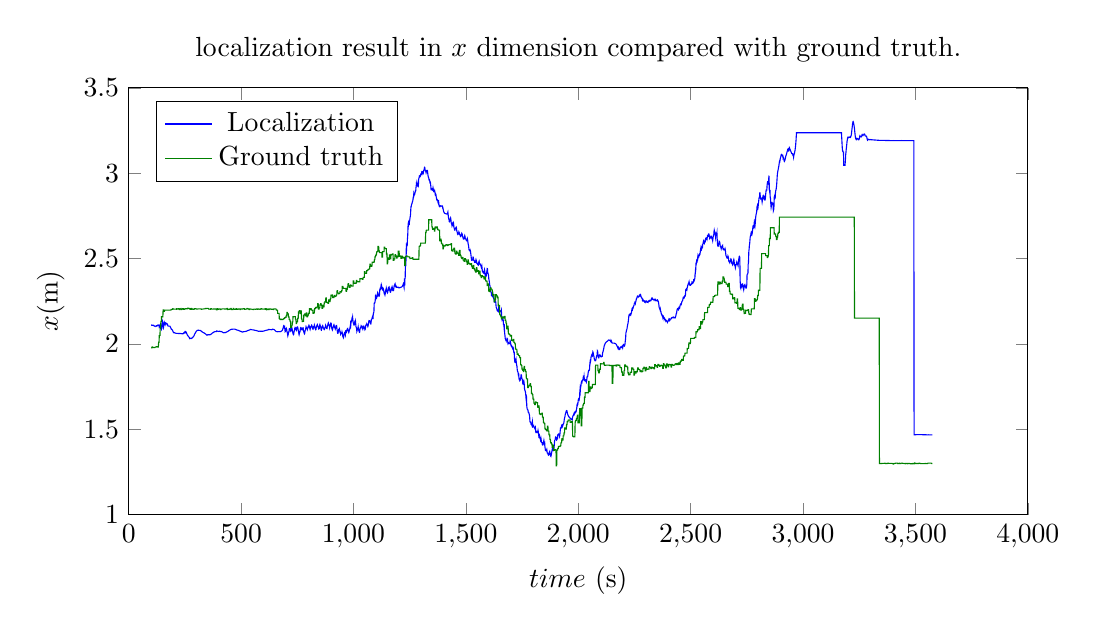
\begin{tikzpicture}

\begin{axis}[
title={localization result in $x$ dimension compared with ground truth.},
xlabel={$time$ (s)},
ylabel={$x$(m)},
xmin=0, xmax=4000,
ymin=1, ymax=3.5,
axis on top,
width=13cm,
height=7cm,
legend style={at={(0.03,0.97)}, anchor=north west},
legend entries={{Localization},{Ground truth}}
]
\addplot [blue]
coordinates {
(100,2.10860419273376)
(101,2.10898423194885)
(102,2.11037564277649)
(103,2.11026835441589)
(104,2.10878705978394)
(105,2.10954546928406)
(106,2.10925936698914)
(107,2.10832190513611)
(108,2.1081645488739)
(109,2.10843086242676)
(110,2.10911822319031)
(111,2.10812854766846)
(112,2.10576224327087)
(113,2.10441875457764)
(114,2.10478496551514)
(115,2.10469770431519)
(116,2.10330510139465)
(117,2.10335493087769)
(118,2.10207676887512)
(119,2.10371851921082)
(120,2.10355687141418)
(121,2.10361289978027)
(122,2.10475564002991)
(123,2.10612964630127)
(124,2.10509705543518)
(125,2.10397100448608)
(126,2.10540246963501)
(127,2.10582804679871)
(128,2.10750341415405)
(129,2.10901165008545)
(130,2.11122488975525)
(131,2.11111879348755)
(132,2.11091732978821)
(133,2.11010527610779)
(134,2.10654950141907)
(135,2.10401272773743)
(136,2.09742474555969)
(137,2.09931993484497)
(138,2.10469317436218)
(139,2.10947036743164)
(140,2.11371898651123)
(141,2.11413955688477)
(142,2.1021466255188)
(143,2.09374308586121)
(144,2.08719801902771)
(145,2.08447766304016)
(146,2.0911021232605)
(147,2.10218477249146)
(148,2.11740946769714)
(149,2.12458848953247)
(150,2.13038659095764)
(151,2.11885094642639)
(152,2.10974788665771)
(153,2.09638023376465)
(154,2.09196925163269)
(155,2.09639024734497)
(156,2.10862684249878)
(157,2.12358975410461)
(158,2.12701654434204)
(159,2.12135696411133)
(160,2.1179530620575)
(161,2.11739373207092)
(162,2.11376237869263)
(163,2.11985898017883)
(164,2.12345814704895)
(165,2.12262940406799)
(166,2.11907434463501)
(167,2.11709976196289)
(168,2.11750650405884)
(169,2.11917233467102)
(170,2.11891412734985)
(171,2.11693787574768)
(172,2.11196970939636)
(173,2.11269450187683)
(174,2.10922455787659)
(175,2.10419750213623)
(176,2.1038281917572)
(177,2.10405802726746)
(178,2.10401034355164)
(179,2.10383057594299)
(180,2.10397124290466)
(181,2.10414719581604)
(182,2.10423374176025)
(183,2.10414338111877)
(184,2.10087418556213)
(185,2.09872984886169)
(186,2.09600734710693)
(187,2.09388327598572)
(188,2.09095311164856)
(189,2.08753538131714)
(190,2.08620953559875)
(191,2.08498024940491)
(192,2.08411026000977)
(193,2.08310031890869)
(194,2.08126544952393)
(195,2.07866597175598)
(196,2.07632207870483)
(197,2.07364559173584)
(198,2.06916737556458)
(199,2.06723237037659)
(200,2.06679654121399)
(201,2.06459760665894)
(202,2.06495547294617)
(203,2.06489157676697)
(204,2.06436324119568)
(205,2.06479835510254)
(206,2.06396317481995)
(207,2.0635027885437)
(208,2.06314659118652)
(209,2.06303119659424)
(210,2.06249475479126)
(211,2.06137442588806)
(212,2.06156587600708)
(213,2.06157469749451)
(214,2.06158375740051)
(215,2.06130146980286)
(216,2.06170606613159)
(217,2.0615291595459)
(218,2.06130504608154)
(219,2.06138134002686)
(220,2.06074953079224)
(221,2.06083011627197)
(222,2.06106424331665)
(223,2.06081223487854)
(224,2.06129145622253)
(225,2.06114220619202)
(226,2.0609564781189)
(227,2.06115293502808)
(228,2.06101155281067)
(229,2.06090235710144)
(230,2.0605480670929)
(231,2.06042814254761)
(232,2.06032276153564)
(233,2.06017565727234)
(234,2.06017184257507)
(235,2.05970549583435)
(236,2.05973672866821)
(237,2.05915808677673)
(238,2.05890369415283)
(239,2.05897116661072)
(240,2.0586884021759)
(241,2.0591127872467)
(242,2.05887150764465)
(243,2.06079173088074)
(244,2.06260800361633)
(245,2.06264996528625)
(246,2.06527709960938)
(247,2.06709337234497)
(248,2.06434416770935)
(249,2.06358170509338)
(250,2.06294965744019)
(251,2.06376147270203)
(252,2.07242751121521)
(253,2.07182168960571)
(254,2.07117533683777)
(255,2.07057452201843)
(256,2.06781935691833)
(257,2.06404590606689)
(258,2.060631275177)
(259,2.05828833580017)
(260,2.05390286445618)
(261,2.05163192749023)
(262,2.05002808570862)
(263,2.04733800888062)
(264,2.04609680175781)
(265,2.04476928710938)
(266,2.04271507263184)
(267,2.04080414772034)
(268,2.03937697410583)
(269,2.03819394111633)
(270,2.03683543205261)
(271,2.03145456314087)
(272,2.03214740753174)
(273,2.03190493583679)
(274,2.03199410438538)
(275,2.03157591819763)
(276,2.0323441028595)
(277,2.03121304512024)
(278,2.03123021125793)
(279,2.03270721435547)
(280,2.03290796279907)
(281,2.03295421600342)
(282,2.03388643264771)
(283,2.03643655776978)
(284,2.03793525695801)
(285,2.03841328620911)
(286,2.04012870788574)
(287,2.04077982902527)
(288,2.04347109794617)
(289,2.04508948326111)
(290,2.04617309570312)
(291,2.04871082305908)
(292,2.05252695083618)
(293,2.05595707893372)
(294,2.05902481079102)
(295,2.06085014343262)
(296,2.06327104568481)
(297,2.06627058982849)
(298,2.06822299957275)
(299,2.06924724578857)
(300,2.07162714004517)
(301,2.07374715805054)
(302,2.07545614242554)
(303,2.07628202438354)
(304,2.07733774185181)
(305,2.07851147651672)
(306,2.07923936843872)
(307,2.07944512367249)
(308,2.07960605621338)
(309,2.0805389881134)
(310,2.07927274703979)
(311,2.07949542999268)
(312,2.07921481132507)
(313,2.07929277420044)
(314,2.07938671112061)
(315,2.07923483848572)
(316,2.07938361167908)
(317,2.07933664321899)
(318,2.07915139198303)
(319,2.0782151222229)
(320,2.07787775993347)
(321,2.07627081871033)
(322,2.07553339004517)
(323,2.07447218894958)
(324,2.072425365448)
(325,2.07127547264099)
(326,2.07155299186707)
(327,2.07059335708618)
(328,2.06938314437866)
(329,2.06828784942627)
(330,2.06763362884521)
(331,2.06701374053955)
(332,2.06628489494324)
(333,2.06617617607117)
(334,2.06487560272217)
(335,2.06369566917419)
(336,2.06319808959961)
(337,2.0623824596405)
(338,2.06087255477905)
(339,2.06048989295959)
(340,2.05957055091858)
(341,2.05892443656921)
(342,2.05748724937439)
(343,2.05637979507446)
(344,2.05525922775269)
(345,2.05391550064087)
(346,2.05289578437805)
(347,2.05142688751221)
(348,2.05205154418945)
(349,2.05250000953674)
(350,2.05303072929382)
(351,2.05224919319153)
(352,2.05314064025879)
(353,2.05267119407654)
(354,2.0532214641571)
(355,2.05387496948242)
(356,2.05368185043335)
(357,2.05344200134277)
(358,2.05297994613647)
(359,2.05340075492859)
(360,2.05366110801697)
(361,2.05329513549805)
(362,2.05356645584106)
(363,2.05409741401672)
(364,2.05480456352234)
(365,2.0556116104126)
(366,2.0564706325531)
(367,2.05743145942688)
(368,2.05870652198792)
(369,2.059818983078)
(370,2.0611789226532)
(371,2.06222796440125)
(372,2.06357789039612)
(373,2.06399607658386)
(374,2.06482887268066)
(375,2.06529569625854)
(376,2.06636095046997)
(377,2.06745791435242)
(378,2.06821084022522)
(379,2.06907486915588)
(380,2.07011103630066)
(381,2.07038354873657)
(382,2.07110738754272)
(383,2.07169437408447)
(384,2.07207632064819)
(385,2.07196307182312)
(386,2.07199096679688)
(387,2.07189798355103)
(388,2.0719621181488)
(389,2.07206392288208)
(390,2.07200026512146)
(391,2.07600927352905)
(392,2.07606482505798)
(393,2.07514023780823)
(394,2.07495999336243)
(395,2.07406783103943)
(396,2.07341909408569)
(397,2.07311153411865)
(398,2.0729866027832)
(399,2.07273197174072)
(400,2.07348370552063)
(401,2.07362747192383)
(402,2.07363414764404)
(403,2.07392001152039)
(404,2.07402968406677)
(405,2.07339692115784)
(406,2.0727219581604)
(407,2.07276821136475)
(408,2.07262229919434)
(409,2.07190084457397)
(410,2.07233047485352)
(411,2.07214450836182)
(412,2.0721538066864)
(413,2.07145404815674)
(414,2.07070922851562)
(415,2.07048416137695)
(416,2.07003331184387)
(417,2.06913256645203)
(418,2.06751036643982)
(419,2.06672430038452)
(420,2.06588053703308)
(421,2.06602382659912)
(422,2.06546258926392)
(423,2.06559348106384)
(424,2.06512928009033)
(425,2.06532406806946)
(426,2.06571412086487)
(427,2.06638073921204)
(428,2.06656646728516)
(429,2.06563949584961)
(430,2.06552600860596)
(431,2.06721973419189)
(432,2.06723380088806)
(433,2.06799840927124)
(434,2.06834530830383)
(435,2.06929230690002)
(436,2.06981897354126)
(437,2.07066440582275)
(438,2.07153964042664)
(439,2.07172322273254)
(440,2.07251501083374)
(441,2.07295727729797)
(442,2.07386374473572)
(443,2.07469534873962)
(444,2.07557129859924)
(445,2.07665657997131)
(446,2.0779128074646)
(447,2.07876324653625)
(448,2.07945990562439)
(449,2.08017587661743)
(450,2.08087611198425)
(451,2.08180546760559)
(452,2.08232808113098)
(453,2.08279347419739)
(454,2.08343148231506)
(455,2.0841851234436)
(456,2.08487224578857)
(457,2.08537840843201)
(458,2.08591246604919)
(459,2.08623909950256)
(460,2.08541321754456)
(461,2.08562231063843)
(462,2.08600378036499)
(463,2.08632349967957)
(464,2.08654308319092)
(465,2.08624982833862)
(466,2.08625245094299)
(467,2.08627653121948)
(468,2.08619666099548)
(469,2.08631634712219)
(470,2.08644342422485)
(471,2.08645749092102)
(472,2.08625483512878)
(473,2.08570790290833)
(474,2.08533549308777)
(475,2.08495759963989)
(476,2.08400940895081)
(477,2.08358526229858)
(478,2.08307600021362)
(479,2.08249187469482)
(480,2.08211469650269)
(481,2.08170533180237)
(482,2.08056783676147)
(483,2.08063817024231)
(484,2.08047008514404)
(485,2.07996368408203)
(486,2.07973980903625)
(487,2.07906079292297)
(488,2.07873463630676)
(489,2.07829475402832)
(490,2.07824754714966)
(491,2.07734251022339)
(492,2.07648706436157)
(493,2.07560348510742)
(494,2.07475519180298)
(495,2.07428002357483)
(496,2.0743043422699)
(497,2.07377481460571)
(498,2.07364273071289)
(499,2.07360482215881)
(500,2.0726912021637)
(501,2.07231950759888)
(502,2.07172036170959)
(503,2.07022714614868)
(504,2.06972980499268)
(505,2.06982231140137)
(506,2.06963920593262)
(507,2.0695104598999)
(508,2.06965327262878)
(509,2.07042241096497)
(510,2.07144975662231)
(511,2.0716028213501)
(512,2.0718400478363)
(513,2.07201886177063)
(514,2.07172632217407)
(515,2.07154059410095)
(516,2.0720579624176)
(517,2.07216167449951)
(518,2.07227730751038)
(519,2.07302761077881)
(520,2.07301425933838)
(521,2.07339644432068)
(522,2.07370829582214)
(523,2.07384967803955)
(524,2.07447671890259)
(525,2.07522821426392)
(526,2.07565951347351)
(527,2.07638144493103)
(528,2.07706809043884)
(529,2.07753491401672)
(530,2.07821917533875)
(531,2.07876539230347)
(532,2.07902264595032)
(533,2.07941746711731)
(534,2.0799286365509)
(535,2.08051037788391)
(536,2.08055400848389)
(537,2.0809953212738)
(538,2.08125114440918)
(539,2.08267688751221)
(540,2.08347320556641)
(541,2.08429479598999)
(542,2.08425116539001)
(543,2.08406090736389)
(544,2.08383750915527)
(545,2.08363199234009)
(546,2.08334493637085)
(547,2.08306193351746)
(548,2.08312487602234)
(549,2.08230328559875)
(550,2.08218002319336)
(551,2.08229374885559)
(552,2.0823655128479)
(553,2.08212900161743)
(554,2.08178019523621)
(555,2.08137774467468)
(556,2.0812611579895)
(557,2.08118104934692)
(558,2.08094263076782)
(559,2.08055329322815)
(560,2.08007287979126)
(561,2.07958602905273)
(562,2.0793821811676)
(563,2.07924222946167)
(564,2.07877612113953)
(565,2.07856798171997)
(566,2.07827234268188)
(567,2.07811164855957)
(568,2.07772588729858)
(569,2.07724857330322)
(570,2.07667446136475)
(571,2.07617926597595)
(572,2.0758159160614)
(573,2.07554841041565)
(574,2.07511043548584)
(575,2.07463788986206)
(576,2.07421445846558)
(577,2.07393193244934)
(578,2.07385587692261)
(579,2.07331371307373)
(580,2.07358765602112)
(581,2.07374119758606)
(582,2.07452654838562)
(583,2.07486176490784)
(584,2.07458758354187)
(585,2.07416081428528)
(586,2.07423830032349)
(587,2.07433724403381)
(588,2.07387852668762)
(589,2.07380414009094)
(590,2.07374334335327)
(591,2.07354855537415)
(592,2.07357954978943)
(593,2.07365274429321)
(594,2.07359051704407)
(595,2.07370948791504)
(596,2.07398629188538)
(597,2.0741286277771)
(598,2.07440733909607)
(599,2.07458710670471)
(600,2.07498002052307)
(601,2.07536578178406)
(602,2.07567453384399)
(603,2.07601475715637)
(604,2.07666492462158)
(605,2.07708215713501)
(606,2.07751417160034)
(607,2.0776960849762)
(608,2.07805180549622)
(609,2.07867765426636)
(610,2.07899188995361)
(611,2.07909059524536)
(612,2.07923936843872)
(613,2.07983827590942)
(614,2.08013486862183)
(615,2.08050799369812)
(616,2.08088636398315)
(617,2.08096742630005)
(618,2.08144521713257)
(619,2.08174324035645)
(620,2.08208799362183)
(621,2.08256554603577)
(622,2.08408117294312)
(623,2.08414173126221)
(624,2.08470439910889)
(625,2.08474612236023)
(626,2.08411908149719)
(627,2.08373141288757)
(628,2.08349251747131)
(629,2.0834002494812)
(630,2.08343720436096)
(631,2.08337187767029)
(632,2.08339095115662)
(633,2.08331155776978)
(634,2.08325791358948)
(635,2.08318734169006)
(636,2.0827329158783)
(637,2.08276391029358)
(638,2.08423566818237)
(639,2.0853419303894)
(640,2.0858736038208)
(641,2.08563327789307)
(642,2.08540630340576)
(643,2.08520007133484)
(644,2.08516049385071)
(645,2.08493685722351)
(646,2.08429551124573)
(647,2.08319115638733)
(648,2.08236622810364)
(649,2.08123469352722)
(650,2.0804078578949)
(651,2.07867050170898)
(652,2.07793307304382)
(653,2.07652235031128)
(654,2.07544898986816)
(655,2.07392430305481)
(656,2.07268524169922)
(657,2.07148838043213)
(658,2.07159376144409)
(659,2.07155632972717)
(660,2.07156729698181)
(661,2.07127094268799)
(662,2.07147574424744)
(663,2.07147312164307)
(664,2.07128977775574)
(665,2.07147979736328)
(666,2.07153606414795)
(667,2.07163596153259)
(668,2.07183337211609)
(669,2.07175803184509)
(670,2.07168984413147)
(671,2.07183837890625)
(672,2.07142972946167)
(673,2.07130885124207)
(674,2.0715274810791)
(675,2.07180285453796)
(676,2.07181334495544)
(677,2.07262992858887)
(678,2.07373929023743)
(679,2.07458114624023)
(680,2.07534885406494)
(681,2.0765483379364)
(682,2.07733273506165)
(683,2.07895874977112)
(684,2.08119034767151)
(685,2.08451271057129)
(686,2.08859348297119)
(687,2.09211587905884)
(688,2.09827184677124)
(689,2.10469841957092)
(690,2.10674786567688)
(691,2.10461282730103)
(692,2.09452795982361)
(693,2.09193205833435)
(694,2.0950493812561)
(695,2.08271408081055)
(696,2.07119560241699)
(697,2.07241368293762)
(698,2.08049249649048)
(699,2.08731269836426)
(700,2.08587050437927)
(701,2.08427906036377)
(702,2.08841824531555)
(703,2.0843391418457)
(704,2.07383275032043)
(705,2.06727719306946)
(706,2.06255054473877)
(707,2.05573987960815)
(708,2.04750037193298)
(709,2.05220937728882)
(710,2.05662298202515)
(711,2.0675573348999)
(712,2.07082653045654)
(713,2.07076072692871)
(714,2.08453726768494)
(715,2.08934354782104)
(716,2.088951587677)
(717,2.08404779434204)
(718,2.08249521255493)
(719,2.08690714836121)
(720,2.08173656463623)
(721,2.07510495185852)
(722,2.0768449306488)
(723,2.08227229118347)
(724,2.08704996109009)
(725,2.08430409431458)
(726,2.08480477333069)
(727,2.08755040168762)
(728,2.07948160171509)
(729,2.07211565971375)
(730,2.06623983383179)
(731,2.05995607376099)
(732,2.05533909797668)
(733,2.05382227897644)
(734,2.05622601509094)
(735,2.06610083580017)
(736,2.07543420791626)
(737,2.07630467414856)
(738,2.08353137969971)
(739,2.09226632118225)
(740,2.09500980377197)
(741,2.0926616191864)
(742,2.08734059333801)
(743,2.08874559402466)
(744,2.09115076065063)
(745,2.08290076255798)
(746,2.08021354675293)
(747,2.08539795875549)
(748,2.09263610839844)
(749,2.09332895278931)
(750,2.09361410140991)
(751,2.09838581085205)
(752,2.09753727912903)
(753,2.09031939506531)
(754,2.08212423324585)
(755,2.07487106323242)
(756,2.07066226005554)
(757,2.05792140960693)
(758,2.05326294898987)
(759,2.05797052383423)
(760,2.06621170043945)
(761,2.07180166244507)
(762,2.07124018669128)
(763,2.08002161979675)
(764,2.09342408180237)
(765,2.09458684921265)
(766,2.09020400047302)
(767,2.08914351463318)
(768,2.09272527694702)
(769,2.09190440177917)
(770,2.08266043663025)
(771,2.08193969726562)
(772,2.08706617355347)
(773,2.09105753898621)
(774,2.0899384021759)
(775,2.09093594551086)
(776,2.09223127365112)
(777,2.08500051498413)
(778,2.07601523399353)
(779,2.07058167457581)
(780,2.06567192077637)
(781,2.06159687042236)
(782,2.05902624130249)
(783,2.06192469596863)
(784,2.07124042510986)
(785,2.07873249053955)
(786,2.080641746521)
(787,2.08250904083252)
(788,2.09355211257935)
(789,2.10021090507507)
(790,2.09686732292175)
(791,2.09327149391174)
(792,2.09075164794922)
(793,2.09149146080017)
(794,2.09196925163269)
(795,2.08567929267883)
(796,2.0905556678772)
(797,2.0947802066803)
(798,2.09967660903931)
(799,2.10025858879089)
(800,2.10242795944214)
(801,2.10616898536682)
(802,2.1020143032074)
(803,2.10493421554565)
(804,2.09970498085022)
(805,2.09745621681213)
(806,2.08814096450806)
(807,2.08414506912231)
(808,2.08899021148682)
(809,2.092609167099)
(810,2.10073590278625)
(811,2.10121536254883)
(812,2.10147523880005)
(813,2.10756921768188)
(814,2.10987663269043)
(815,2.10767531394958)
(816,2.0959300994873)
(817,2.09527826309204)
(818,2.09523582458496)
(819,2.08655476570129)
(820,2.08570098876953)
(821,2.09064483642578)
(822,2.10025262832642)
(823,2.10170483589172)
(824,2.10007357597351)
(825,2.10218548774719)
(826,2.10927772521973)
(827,2.10438680648804)
(828,2.09979271888733)
(829,2.09143805503845)
(830,2.09205174446106)
(831,2.08833956718445)
(832,2.0827329158783)
(833,2.08371615409851)
(834,2.09217762947083)
(835,2.10246443748474)
(836,2.10413527488708)
(837,2.10436081886292)
(838,2.10985732078552)
(839,2.11274147033691)
(840,2.10840940475464)
(841,2.10245943069458)
(842,2.10107088088989)
(843,2.09974455833435)
(844,2.09171009063721)
(845,2.08856558799744)
(846,2.09151434898376)
(847,2.09733080863953)
(848,2.10244989395142)
(849,2.0978376865387)
(850,2.10424709320068)
(851,2.1116635799408)
(852,2.10781025886536)
(853,2.1010377407074)
(854,2.09813213348389)
(855,2.09605073928833)
(856,2.08158373832703)
(857,2.08051300048828)
(858,2.08586525917053)
(859,2.09153127670288)
(860,2.09946250915527)
(861,2.09837079048157)
(862,2.10364603996277)
(863,2.10625076293945)
(864,2.10307550430298)
(865,2.09708142280579)
(866,2.09262180328369)
(867,2.09238576889038)
(868,2.08942794799805)
(869,2.08346104621887)
(870,2.08298587799072)
(871,2.08484697341919)
(872,2.09322500228882)
(873,2.09498953819275)
(874,2.09478878974915)
(875,2.10159420967102)
(876,2.10854172706604)
(877,2.10465121269226)
(878,2.09770750999451)
(879,2.09533286094666)
(880,2.09327292442322)
(881,2.0889937877655)
(882,2.08892869949341)
(883,2.09574818611145)
(884,2.10444259643555)
(885,2.10864019393921)
(886,2.11146450042725)
(887,2.11917018890381)
(888,2.12219047546387)
(889,2.11669874191284)
(890,2.11036419868469)
(891,2.10790991783142)
(892,2.1088502407074)
(893,2.10176372528076)
(894,2.09467005729675)
(895,2.10205507278442)
(896,2.10835385322571)
(897,2.11331415176392)
(898,2.11000084877014)
(899,2.11326003074646)
(900,2.12079882621765)
(901,2.11924481391907)
(902,2.10602855682373)
(903,2.09303116798401)
(904,2.09038877487183)
(905,2.08493423461914)
(906,2.08093690872192)
(907,2.08442521095276)
(908,2.09031176567078)
(909,2.09763932228088)
(910,2.09869265556335)
(911,2.10221934318542)
(912,2.1096568107605)
(913,2.11215758323669)
(914,2.10795664787292)
(915,2.09849286079407)
(916,2.09606695175171)
(917,2.0966796875)
(918,2.09075236320496)
(919,2.08685922622681)
(920,2.09070658683777)
(921,2.0976722240448)
(922,2.10244703292847)
(923,2.10056471824646)
(924,2.10601115226746)
(925,2.10683679580688)
(926,2.09226751327515)
(927,2.08584356307983)
(928,2.07493209838867)
(929,2.0672242641449)
(930,2.06215023994446)
(931,2.06192302703857)
(932,2.06819081306458)
(933,2.0729718208313)
(934,2.08038663864136)
(935,2.07919883728027)
(936,2.08483242988586)
(937,2.08919239044189)
(938,2.08560800552368)
(939,2.07471394538879)
(940,2.06967258453369)
(941,2.07073926925659)
(942,2.06506443023682)
(943,2.05582094192505)
(944,2.05848431587219)
(945,2.06310987472534)
(946,2.0635883808136)
(947,2.06314039230347)
(948,2.06343102455139)
(949,2.07029843330383)
(950,2.06542348861694)
(951,2.06161046028137)
(952,2.04691457748413)
(953,2.04628825187683)
(954,2.03868103027344)
(955,2.03506255149841)
(956,2.03874826431274)
(957,2.0459406375885)
(958,2.05405950546265)
(959,2.05330348014832)
(960,2.05905604362488)
(961,2.06710290908813)
(962,2.06837725639343)
(963,2.06296706199646)
(964,2.056476354599)
(965,2.07617664337158)
(966,2.07577729225159)
(967,2.06664395332336)
(968,2.06606292724609)
(969,2.07125616073608)
(970,2.07975006103516)
(971,2.07986116409302)
(972,2.08141088485718)
(973,2.08947491645813)
(974,2.09039354324341)
(975,2.08352160453796)
(976,2.07798552513123)
(977,2.07650995254517)
(978,2.07048225402832)
(979,2.06660652160645)
(980,2.07037854194641)
(981,2.07514548301697)
(982,2.08440613746643)
(983,2.08521866798401)
(984,2.09023761749268)
(985,2.09828758239746)
(986,2.09689497947693)
(987,2.11540842056274)
(988,2.10991978645325)
(989,2.12420010566711)
(990,2.13319301605225)
(991,2.13159847259521)
(992,2.13492655754089)
(993,2.14822816848755)
(994,2.15312218666077)
(995,2.15138268470764)
(996,2.15777730941772)
(997,2.14380693435669)
(998,2.1343834400177)
(999,2.12279009819031)
(1000,2.11967778205872)
(1001,2.11560368537903)
(1002,2.11032295227051)
(1003,2.11002850532532)
(1004,2.11498856544495)
(1005,2.12342953681946)
(1006,2.11822032928467)
(1007,2.11867880821228)
(1008,2.1230103969574)
(1009,2.13022184371948)
(1010,2.11634993553162)
(1011,2.10236811637878)
(1012,2.09871482849121)
(1013,2.09264421463013)
(1014,2.08796620368958)
(1015,2.07252788543701)
(1016,2.07580614089966)
(1017,2.08617973327637)
(1018,2.08957028388977)
(1019,2.08760619163513)
(1020,2.09081101417542)
(1021,2.09933876991272)
(1022,2.09004950523376)
(1023,2.08043909072876)
(1024,2.07750964164734)
(1025,2.07401943206787)
(1026,2.06824350357056)
(1027,2.06764626502991)
(1028,2.07415771484375)
(1029,2.08608651161194)
(1030,2.09315180778503)
(1031,2.09277057647705)
(1032,2.0960841178894)
(1033,2.09998154640198)
(1034,2.10600662231445)
(1035,2.10385513305664)
(1036,2.09852194786072)
(1037,2.09809064865112)
(1038,2.09767436981201)
(1039,2.09025835990906)
(1040,2.08877229690552)
(1041,2.09427404403687)
(1042,2.08809161186218)
(1043,2.09286999702454)
(1044,2.09274387359619)
(1045,2.09980416297913)
(1046,2.10294389724731)
(1047,2.0997326374054)
(1048,2.09426593780518)
(1049,2.0913507938385)
(1050,2.08952784538269)
(1051,2.08266687393188)
(1052,2.08466172218323)
(1053,2.09088325500488)
(1054,2.10281658172607)
(1055,2.10929417610168)
(1056,2.1092586517334)
(1057,2.11189270019531)
(1058,2.11444473266602)
(1059,2.1177613735199)
(1060,2.11420297622681)
(1061,2.11012244224548)
(1062,2.11023950576782)
(1063,2.1056342124939)
(1064,2.10158467292786)
(1065,2.10469508171082)
(1066,2.11211585998535)
(1067,2.12101459503174)
(1068,2.12981033325195)
(1069,2.12703061103821)
(1070,2.12736415863037)
(1071,2.13558340072632)
(1072,2.13590669631958)
(1073,2.13048529624939)
(1074,2.1275520324707)
(1075,2.1273500919342)
(1076,2.1184253692627)
(1077,2.11721873283386)
(1078,2.12183403968811)
(1079,2.13373470306396)
(1080,2.14323306083679)
(1081,2.14453148841858)
(1082,2.14493441581726)
(1083,2.15286779403687)
(1084,2.15701341629028)
(1085,2.15336322784424)
(1086,2.14897322654724)
(1087,2.14874076843262)
(1088,2.17478013038635)
(1089,2.17920422554016)
(1090,2.18373608589172)
(1091,2.19026660919189)
(1092,2.23563241958618)
(1093,2.23933911323547)
(1094,2.23875951766968)
(1095,2.24201703071594)
(1096,2.24671483039856)
(1097,2.25864934921265)
(1098,2.27970051765442)
(1099,2.27629971504211)
(1100,2.27755689620972)
(1101,2.26710104942322)
(1102,2.26556277275085)
(1103,2.26780676841736)
(1104,2.27858304977417)
(1105,2.28467965126038)
(1106,2.2814724445343)
(1107,2.280757188797)
(1108,2.30021286010742)
(1109,2.2975287437439)
(1110,2.29247856140137)
(1111,2.28707695007324)
(1112,2.2846941947937)
(1113,2.28077626228333)
(1114,2.28023719787598)
(1115,2.28031468391418)
(1116,2.29223084449768)
(1117,2.31668829917908)
(1118,2.32124924659729)
(1119,2.31797361373901)
(1120,2.3209331035614)
(1121,2.3250515460968)
(1122,2.33449554443359)
(1123,2.32836008071899)
(1124,2.33144354820251)
(1125,2.34154868125916)
(1126,2.33518815040588)
(1127,2.32674813270569)
(1128,2.32276082038879)
(1129,2.32959675788879)
(1130,2.32955098152161)
(1131,2.32790493965149)
(1132,2.31952881813049)
(1133,2.32129287719727)
(1134,2.31766510009766)
(1135,2.30678224563599)
(1136,2.30084252357483)
(1137,2.29255056381226)
(1138,2.29107522964478)
(1139,2.28989124298096)
(1140,2.28610610961914)
(1141,2.29241991043091)
(1142,2.30404162406921)
(1143,2.31125211715698)
(1144,2.30942869186401)
(1145,2.31810975074768)
(1146,2.32703852653503)
(1147,2.32187223434448)
(1148,2.31378698348999)
(1149,2.30979800224304)
(1150,2.30393195152283)
(1151,2.29880952835083)
(1152,2.30102300643921)
(1153,2.30702257156372)
(1154,2.31743597984314)
(1155,2.32443118095398)
(1156,2.32006478309631)
(1157,2.31867694854736)
(1158,2.32530856132507)
(1159,2.32878160476685)
(1160,2.32102012634277)
(1161,2.31609702110291)
(1162,2.31233906745911)
(1163,2.30618619918823)
(1164,2.30254936218262)
(1165,2.30289602279663)
(1166,2.30922317504883)
(1167,2.31806516647339)
(1168,2.32479906082153)
(1169,2.32246661186218)
(1170,2.32028031349182)
(1171,2.32810974121094)
(1172,2.33360290527344)
(1173,2.32848453521729)
(1174,2.32112336158752)
(1175,2.31867980957031)
(1176,2.3116135597229)
(1177,2.31198668479919)
(1178,2.312180519104)
(1179,2.32002472877502)
(1180,2.33087992668152)
(1181,2.33941078186035)
(1182,2.33958292007446)
(1183,2.34447693824768)
(1184,2.34894490242004)
(1185,2.3517746925354)
(1186,2.34495425224304)
(1187,2.33698558807373)
(1188,2.33498883247375)
(1189,2.34010863304138)
(1190,2.3375141620636)
(1191,2.33246994018555)
(1192,2.33170580863953)
(1193,2.33092951774597)
(1194,2.33139395713806)
(1195,2.33201003074646)
(1196,2.33228135108948)
(1197,2.33252668380737)
(1198,2.33163595199585)
(1199,2.33030247688293)
(1200,2.33167934417725)
(1201,2.33058667182922)
(1202,2.32986283302307)
(1203,2.3285014629364)
(1204,2.32840776443481)
(1205,2.32853984832764)
(1206,2.32888603210449)
(1207,2.33010506629944)
(1208,2.33086729049683)
(1209,2.33103084564209)
(1210,2.33121800422668)
(1211,2.33174180984497)
(1212,2.33217000961304)
(1213,2.33271217346191)
(1214,2.3333523273468)
(1215,2.33457398414612)
(1216,2.33527445793152)
(1217,2.3371274471283)
(1218,2.33947372436523)
(1219,2.34150862693787)
(1220,2.34501934051514)
(1221,2.34899663925171)
(1222,2.35260796546936)
(1223,2.34920310974121)
(1224,2.33846664428711)
(1225,2.33158707618713)
(1226,2.35819244384766)
(1227,2.35179448127747)
(1228,2.349604845047)
(1229,2.38265562057495)
(1230,2.38754677772522)
(1231,2.4573655128479)
(1232,2.45681142807007)
(1233,2.46068859100342)
(1234,2.5228168964386)
(1235,2.56020498275757)
(1236,2.55302333831787)
(1237,2.57865571975708)
(1238,2.57514786720276)
(1239,2.57830429077148)
(1240,2.61445450782776)
(1241,2.63021564483643)
(1242,2.65662217140198)
(1243,2.70006108283997)
(1244,2.70690894126892)
(1245,2.69657349586487)
(1246,2.70351243019104)
(1247,2.69822072982788)
(1248,2.6993100643158)
(1249,2.71706819534302)
(1250,2.72219395637512)
(1251,2.7335250377655)
(1252,2.74270939826965)
(1253,2.7505156993866)
(1254,2.76053309440613)
(1255,2.78976440429688)
(1256,2.80383610725403)
(1257,2.80599594116211)
(1258,2.81378936767578)
(1259,2.81900501251221)
(1260,2.82040572166443)
(1261,2.82710003852844)
(1262,2.83191013336182)
(1263,2.8372209072113)
(1264,2.83781099319458)
(1265,2.85029911994934)
(1266,2.85885429382324)
(1267,2.86288261413574)
(1268,2.87566018104553)
(1269,2.86709570884705)
(1270,2.87110424041748)
(1271,2.87671971321106)
(1272,2.87607431411743)
(1273,2.87787389755249)
(1274,2.889324426651)
(1275,2.89478325843811)
(1276,2.89378309249878)
(1277,2.89767694473267)
(1278,2.91555285453796)
(1279,2.9226131439209)
(1280,2.93952083587646)
(1281,2.93247699737549)
(1282,2.93380355834961)
(1283,2.93099164962769)
(1284,2.92634344100952)
(1285,2.92511487007141)
(1286,2.93999147415161)
(1287,2.94643449783325)
(1288,2.94002771377563)
(1289,2.93511962890625)
(1290,2.96261787414551)
(1291,2.97189211845398)
(1292,2.97306418418884)
(1293,2.98119258880615)
(1294,2.97971749305725)
(1295,2.98329091072083)
(1296,2.98235774040222)
(1297,2.98129153251648)
(1298,2.98966526985168)
(1299,2.99495840072632)
(1300,2.99569702148438)
(1301,2.99295401573181)
(1302,2.99215388298035)
(1303,3.00201439857483)
(1304,3.01001477241516)
(1305,3.00989246368408)
(1306,3.00825214385986)
(1307,3.0054874420166)
(1308,3.00039935112)
(1309,2.99436402320862)
(1310,2.99605846405029)
(1311,3.00587821006775)
(1312,3.01487398147583)
(1313,3.01830697059631)
(1314,3.01822257041931)
(1315,3.02618980407715)
(1316,3.03444147109985)
(1317,3.03349447250366)
(1318,3.02669763565063)
(1319,3.01730108261108)
(1320,3.0151469707489)
(1321,3.01528477668762)
(1322,3.00812911987305)
(1323,3.00257086753845)
(1324,3.00678944587708)
(1325,3.01217222213745)
(1326,3.01121187210083)
(1327,3.01143860816956)
(1328,3.01620769500732)
(1329,3.01537656784058)
(1330,3.003746509552)
(1331,2.99261832237244)
(1332,2.98366022109985)
(1333,2.9781813621521)
(1334,2.97360610961914)
(1335,2.97093367576599)
(1336,2.96244955062866)
(1337,2.96384429931641)
(1338,2.96189498901367)
(1339,2.95718622207642)
(1340,2.94803333282471)
(1341,2.95027112960815)
(1342,2.94902181625366)
(1343,2.9366466999054)
(1344,2.92422389984131)
(1345,2.9067747592926)
(1346,2.9028468132019)
(1347,2.90344905853271)
(1348,2.90638518333435)
(1349,2.91070747375488)
(1350,2.91046643257141)
(1351,2.9042866230011)
(1352,2.90114259719849)
(1353,2.90298748016357)
(1354,2.91320872306824)
(1355,2.90609526634216)
(1356,2.89880681037903)
(1357,2.8916962146759)
(1358,2.89184093475342)
(1359,2.89434313774109)
(1360,2.89423799514771)
(1361,2.89803981781006)
(1362,2.89155149459839)
(1363,2.88276386260986)
(1364,2.87283325195312)
(1365,2.87417936325073)
(1366,2.87689208984375)
(1367,2.87403297424316)
(1368,2.86262941360474)
(1369,2.85687851905823)
(1370,2.84653234481812)
(1371,2.8438732624054)
(1372,2.83970522880554)
(1373,2.8393349647522)
(1374,2.84231066703796)
(1375,2.84002470970154)
(1376,2.82861852645874)
(1377,2.82492637634277)
(1378,2.82780408859253)
(1379,2.83126616477966)
(1380,2.81845569610596)
(1381,2.80949068069458)
(1382,2.80517983436584)
(1383,2.80353164672852)
(1384,2.80347752571106)
(1385,2.80389761924744)
(1386,2.80827212333679)
(1387,2.80776476860046)
(1388,2.80870008468628)
(1389,2.80762672424316)
(1390,2.80788445472717)
(1391,2.80822324752808)
(1392,2.80866980552673)
(1393,2.80866885185242)
(1394,2.80577611923218)
(1395,2.80566740036011)
(1396,2.80644464492798)
(1397,2.79677438735962)
(1398,2.79717803001404)
(1399,2.78910112380981)
(1400,2.78171181678772)
(1401,2.77621936798096)
(1402,2.77312874794006)
(1403,2.76899647712708)
(1404,2.76810383796692)
(1405,2.7656581401825)
(1406,2.76534128189087)
(1407,2.76489615440369)
(1408,2.76386690139771)
(1409,2.76357889175415)
(1410,2.7629029750824)
(1411,2.76222705841064)
(1412,2.76189470291138)
(1413,2.76150226593018)
(1414,2.7611448764801)
(1415,2.76085329055786)
(1416,2.76070046424866)
(1417,2.76216793060303)
(1418,2.76355934143066)
(1419,2.76750588417053)
(1420,2.77196860313416)
(1421,2.76031684875488)
(1422,2.74640154838562)
(1423,2.73871517181396)
(1424,2.73235034942627)
(1425,2.72801876068115)
(1426,2.71701049804688)
(1427,2.71555233001709)
(1428,2.71738266944885)
(1429,2.72625684738159)
(1430,2.72659087181091)
(1431,2.73495483398438)
(1432,2.73795175552368)
(1433,2.73140382766724)
(1434,2.72319316864014)
(1435,2.70740938186646)
(1436,2.70611977577209)
(1437,2.70282387733459)
(1438,2.69487810134888)
(1439,2.70097184181213)
(1440,2.70102262496948)
(1441,2.70497250556946)
(1442,2.70095109939575)
(1443,2.70876812934875)
(1444,2.71196222305298)
(1445,2.70842289924622)
(1446,2.69414353370667)
(1447,2.68483757972717)
(1448,2.67805957794189)
(1449,2.67410898208618)
(1450,2.667076587677)
(1451,2.66613984107971)
(1452,2.6696994304657)
(1453,2.67468333244324)
(1454,2.67565703392029)
(1455,2.67794346809387)
(1456,2.68228983879089)
(1457,2.68400454521179)
(1458,2.67850875854492)
(1459,2.66807675361633)
(1460,2.65812253952026)
(1461,2.65602922439575)
(1462,2.65191102027893)
(1463,2.64381051063538)
(1464,2.64045214653015)
(1465,2.64122915267944)
(1466,2.6471631526947)
(1467,2.64855742454529)
(1468,2.65023469924927)
(1469,2.65620541572571)
(1470,2.65314221382141)
(1471,2.64952659606934)
(1472,2.64261937141418)
(1473,2.6387312412262)
(1474,2.63850975036621)
(1475,2.6359531879425)
(1476,2.62936449050903)
(1477,2.63061428070068)
(1478,2.63175344467163)
(1479,2.63724565505981)
(1480,2.6356475353241)
(1481,2.63905954360962)
(1482,2.64746785163879)
(1483,2.64525198936462)
(1484,2.64055514335632)
(1485,2.63189101219177)
(1486,2.62805080413818)
(1487,2.62394237518311)
(1488,2.61878705024719)
(1489,2.61440658569336)
(1490,2.61447644233704)
(1491,2.61825251579285)
(1492,2.61877393722534)
(1493,2.6180408000946)
(1494,2.62963628768921)
(1495,2.63422608375549)
(1496,2.63017177581787)
(1497,2.62188696861267)
(1498,2.61720561981201)
(1499,2.61749792098999)
(1500,2.61476421356201)
(1501,2.6080219745636)
(1502,2.60733819007874)
(1503,2.60891509056091)
(1504,2.60944128036499)
(1505,2.60447239875793)
(1506,2.60618352890015)
(1507,2.61373257637024)
(1508,2.60761404037476)
(1509,2.59601879119873)
(1510,2.58682370185852)
(1511,2.58135962486267)
(1512,2.57499527931213)
(1513,2.56283569335938)
(1514,2.55186700820923)
(1515,2.54941177368164)
(1516,2.54991841316223)
(1517,2.54927754402161)
(1518,2.54553294181824)
(1519,2.54923963546753)
(1520,2.54517507553101)
(1521,2.53927612304688)
(1522,2.52646851539612)
(1523,2.5167384147644)
(1524,2.50448870658875)
(1525,2.49518275260925)
(1526,2.48972344398499)
(1527,2.4895966053009)
(1528,2.49015665054321)
(1529,2.49489212036133)
(1530,2.49417424201965)
(1531,2.49887228012085)
(1532,2.50825643539429)
(1533,2.50739526748657)
(1534,2.49743723869324)
(1535,2.48996329307556)
(1536,2.48803615570068)
(1537,2.48829221725464)
(1538,2.48291993141174)
(1539,2.47770357131958)
(1540,2.4771294593811)
(1541,2.48051166534424)
(1542,2.4832558631897)
(1543,2.48135876655579)
(1544,2.48720169067383)
(1545,2.49331307411194)
(1546,2.48919606208801)
(1547,2.48440861701965)
(1548,2.47477579116821)
(1549,2.47508382797241)
(1550,2.47270441055298)
(1551,2.46845006942749)
(1552,2.46583414077759)
(1553,2.46463418006897)
(1554,2.46791195869446)
(1555,2.47039341926575)
(1556,2.46680927276611)
(1557,2.47461843490601)
(1558,2.48291659355164)
(1559,2.48524260520935)
(1560,2.47491574287415)
(1561,2.46701169013977)
(1562,2.46646571159363)
(1563,2.46903252601624)
(1564,2.46776056289673)
(1565,2.46185684204102)
(1566,2.45984077453613)
(1567,2.45791101455688)
(1568,2.45136737823486)
(1569,2.44764542579651)
(1570,2.45144104957581)
(1571,2.45662832260132)
(1572,2.44520139694214)
(1573,2.43070030212402)
(1574,2.42345356941223)
(1575,2.42404556274414)
(1576,2.42293548583984)
(1577,2.41943597793579)
(1578,2.41504335403442)
(1579,2.41436147689819)
(1580,2.4197371006012)
(1581,2.41714549064636)
(1582,2.42414975166321)
(1583,2.43329381942749)
(1584,2.42731642723083)
(1585,2.41629838943481)
(1586,2.4009575843811)
(1587,2.40055561065674)
(1588,2.4006712436676)
(1589,2.39431953430176)
(1590,2.3947479724884)
(1591,2.40474677085876)
(1592,2.41471147537231)
(1593,2.42174887657166)
(1594,2.4313371181488)
(1595,2.44135594367981)
(1596,2.44055223464966)
(1597,2.42060565948486)
(1598,2.41122794151306)
(1599,2.41004776954651)
(1600,2.4093873500824)
(1601,2.39743304252625)
(1602,2.38163614273071)
(1603,2.37400317192078)
(1604,2.36677193641663)
(1605,2.35718297958374)
(1606,2.343754529953)
(1607,2.34214401245117)
(1608,2.33486747741699)
(1609,2.32014274597168)
(1610,2.30841016769409)
(1611,2.30460238456726)
(1612,2.30419445037842)
(1613,2.3001115322113)
(1614,2.28272366523743)
(1615,2.28261828422546)
(1616,2.28084206581116)
(1617,2.2798023223877)
(1618,2.28426647186279)
(1619,2.28977704048157)
(1620,2.29232549667358)
(1621,2.28246903419495)
(1622,2.26963043212891)
(1623,2.2670590877533)
(1624,2.26731181144714)
(1625,2.26444435119629)
(1626,2.25087451934814)
(1627,2.24580860137939)
(1628,2.24701261520386)
(1629,2.2477707862854)
(1630,2.25252819061279)
(1631,2.24958276748657)
(1632,2.24986815452576)
(1633,2.2428834438324)
(1634,2.22652173042297)
(1635,2.21349048614502)
(1636,2.21209740638733)
(1637,2.20867872238159)
(1638,2.20351552963257)
(1639,2.19622993469238)
(1640,2.19330883026123)
(1641,2.19286227226257)
(1642,2.19440579414368)
(1643,2.1909122467041)
(1644,2.1891725063324)
(1645,2.19854998588562)
(1646,2.21283173561096)
(1647,2.20254302024841)
(1648,2.19347953796387)
(1649,2.19169878959656)
(1650,2.19408965110779)
(1651,2.19435858726501)
(1652,2.19015169143677)
(1653,2.19104313850403)
(1654,2.18949294090271)
(1655,2.19001770019531)
(1656,2.18932199478149)
(1657,2.19282174110413)
(1658,2.19730663299561)
(1659,2.16622400283813)
(1660,2.15676355361938)
(1661,2.14053416252136)
(1662,2.14252901077271)
(1663,2.14417338371277)
(1664,2.14796352386475)
(1665,2.1438422203064)
(1666,2.13978624343872)
(1667,2.11566877365112)
(1668,2.11656856536865)
(1669,2.11451458930969)
(1670,2.09585428237915)
(1671,2.09954071044922)
(1672,2.07151317596436)
(1673,2.05779790878296)
(1674,2.04814481735229)
(1675,2.0315580368042)
(1676,2.03149461746216)
(1677,2.02700304985046)
(1678,2.02046489715576)
(1679,2.02133631706238)
(1680,2.02253675460815)
(1681,2.02307891845703)
(1682,2.01761341094971)
(1683,2.02176737785339)
(1684,2.03109860420227)
(1685,2.02944254875183)
(1686,2.01438236236572)
(1687,2.00482201576233)
(1688,2.00835514068604)
(1689,2.00741863250732)
(1690,2.00468897819519)
(1691,1.99975121021271)
(1692,1.99978637695312)
(1693,2.00172972679138)
(1694,2.00255346298218)
(1695,2.00255823135376)
(1696,2.01085662841797)
(1697,2.01707625389099)
(1698,2.0139045715332)
(1699,2.00582337379456)
(1700,1.99469304084778)
(1701,1.99046802520752)
(1702,1.99195122718811)
(1703,1.99068605899811)
(1704,1.98283100128174)
(1705,1.98060286045074)
(1706,1.98010396957397)
(1707,1.97982442378998)
(1708,1.97075474262238)
(1709,1.97117471694946)
(1710,1.97867596149445)
(1711,1.97627830505371)
(1712,1.96243584156036)
(1713,1.95118367671967)
(1714,1.9506983757019)
(1715,1.95135962963104)
(1716,1.91966819763184)
(1717,1.90421032905579)
(1718,1.89253556728363)
(1719,1.89191019535065)
(1720,1.89833128452301)
(1721,1.89993035793304)
(1722,1.90539360046387)
(1723,1.90995681285858)
(1724,1.89493668079376)
(1725,1.88447034358978)
(1726,1.87428724765778)
(1727,1.87389349937439)
(1728,1.85613059997559)
(1729,1.84482002258301)
(1730,1.83875548839569)
(1731,1.8377126455307)
(1732,1.8328595161438)
(1733,1.82245934009552)
(1734,1.82594299316406)
(1735,1.82506704330444)
(1736,1.80485737323761)
(1737,1.79062759876251)
(1738,1.78908145427704)
(1739,1.79076528549194)
(1740,1.78397381305695)
(1741,1.78550243377686)
(1742,1.7890876531601)
(1743,1.7972891330719)
(1744,1.79802095890045)
(1745,1.81156957149506)
(1746,1.81868755817413)
(1747,1.81780564785004)
(1748,1.80770206451416)
(1749,1.79512190818787)
(1750,1.79419469833374)
(1751,1.79295766353607)
(1752,1.78695738315582)
(1753,1.76863348484039)
(1754,1.76543188095093)
(1755,1.76778471469879)
(1756,1.77432012557983)
(1757,1.77550446987152)
(1758,1.78093016147614)
(1759,1.77396023273468)
(1760,1.75579285621643)
(1761,1.73628389835358)
(1762,1.73082160949707)
(1763,1.72699534893036)
(1764,1.72152459621429)
(1765,1.71901261806488)
(1766,1.70694148540497)
(1767,1.6930547952652)
(1768,1.67653846740723)
(1769,1.6659517288208)
(1770,1.67337226867676)
(1771,1.63586163520813)
(1772,1.62499892711639)
(1773,1.61785340309143)
(1774,1.6165519952774)
(1775,1.61598813533783)
(1776,1.61287999153137)
(1777,1.60246777534485)
(1778,1.59875166416168)
(1779,1.59897255897522)
(1780,1.59745526313782)
(1781,1.59121990203857)
(1782,1.58655428886414)
(1783,1.58219254016876)
(1784,1.5676736831665)
(1785,1.54550635814667)
(1786,1.5416487455368)
(1787,1.54181790351868)
(1788,1.54227244853973)
(1789,1.53653383255005)
(1790,1.52872514724731)
(1791,1.52894520759583)
(1792,1.53029000759125)
(1793,1.52559447288513)
(1794,1.52169477939606)
(1795,1.53288447856903)
(1796,1.54293370246887)
(1797,1.52874040603638)
(1798,1.51610255241394)
(1799,1.5178347826004)
(1800,1.52270019054413)
(1801,1.52307403087616)
(1802,1.51505327224731)
(1803,1.51226508617401)
(1804,1.50970864295959)
(1805,1.50800740718842)
(1806,1.50634980201721)
(1807,1.50364470481873)
(1808,1.50970339775085)
(1809,1.51241409778595)
(1810,1.50279867649078)
(1811,1.48564696311951)
(1812,1.48790812492371)
(1813,1.48833358287811)
(1814,1.48580276966095)
(1815,1.48016571998596)
(1816,1.47989869117737)
(1817,1.48025727272034)
(1818,1.48008096218109)
(1819,1.48005199432373)
(1820,1.48800122737885)
(1821,1.49407613277435)
(1822,1.4874541759491)
(1823,1.47473883628845)
(1824,1.46484172344208)
(1825,1.47166955471039)
(1826,1.47135615348816)
(1827,1.46566069126129)
(1828,1.45815432071686)
(1829,1.44683825969696)
(1830,1.44618368148804)
(1831,1.44272768497467)
(1832,1.4362713098526)
(1833,1.44086146354675)
(1834,1.44675481319427)
(1835,1.4382711648941)
(1836,1.42607986927032)
(1837,1.42309021949768)
(1838,1.42331981658936)
(1839,1.42206883430481)
(1840,1.41109788417816)
(1841,1.40781962871552)
(1842,1.40732979774475)
(1843,1.41196203231812)
(1844,1.4120934009552)
(1845,1.41863536834717)
(1846,1.42884051799774)
(1847,1.43454051017761)
(1848,1.42574763298035)
(1849,1.41454172134399)
(1850,1.40992629528046)
(1851,1.41366147994995)
(1852,1.3942563533783)
(1853,1.38499796390533)
(1854,1.37699568271637)
(1855,1.3770580291748)
(1856,1.37528038024902)
(1857,1.37359476089478)
(1858,1.37573039531708)
(1859,1.37826097011566)
(1860,1.38152658939362)
(1861,1.37259221076965)
(1862,1.36141586303711)
(1863,1.35917913913727)
(1864,1.35858452320099)
(1865,1.35655868053436)
(1866,1.35041785240173)
(1867,1.34920978546143)
(1868,1.35589993000031)
(1869,1.35842549800873)
(1870,1.35644459724426)
(1871,1.3611387014389)
(1872,1.3669410943985)
(1873,1.36979532241821)
(1874,1.36340868473053)
(1875,1.3507239818573)
(1876,1.347412109375)
(1877,1.35090148448944)
(1878,1.34909355640411)
(1879,1.34411466121674)
(1880,1.34828746318817)
(1881,1.35787487030029)
(1882,1.36562609672546)
(1883,1.37213778495789)
(1884,1.37694537639618)
(1885,1.38766252994537)
(1886,1.39548587799072)
(1887,1.39115369319916)
(1888,1.38448429107666)
(1889,1.38875997066498)
(1890,1.38909244537354)
(1891,1.38350009918213)
(1892,1.38915085792542)
(1893,1.40239071846008)
(1894,1.42148125171661)
(1895,1.4330872297287)
(1896,1.43527138233185)
(1897,1.43802511692047)
(1898,1.44624328613281)
(1899,1.45282220840454)
(1900,1.45146834850311)
(1901,1.44542765617371)
(1902,1.44296050071716)
(1903,1.442302942276)
(1904,1.43668127059937)
(1905,1.43815743923187)
(1906,1.44512557983398)
(1907,1.45846974849701)
(1908,1.46246778964996)
(1909,1.45780026912689)
(1910,1.46648812294006)
(1911,1.46746921539307)
(1912,1.4675225019455)
(1913,1.47051453590393)
(1914,1.46813476085663)
(1915,1.46854865550995)
(1916,1.46873271465302)
(1917,1.45890474319458)
(1918,1.46407389640808)
(1919,1.47974967956543)
(1920,1.49469149112701)
(1921,1.5069797039032)
(1922,1.50723743438721)
(1923,1.50910568237305)
(1924,1.50785994529724)
(1925,1.51375472545624)
(1926,1.5217159986496)
(1927,1.52150189876556)
(1928,1.52691280841827)
(1929,1.52716779708862)
(1930,1.51701271533966)
(1931,1.52028155326843)
(1932,1.52519607543945)
(1933,1.52835619449615)
(1934,1.5313515663147)
(1935,1.53415358066559)
(1936,1.53771924972534)
(1937,1.54844224452972)
(1938,1.55807554721832)
(1939,1.5644611120224)
(1940,1.56951093673706)
(1941,1.57560157775879)
(1942,1.58482074737549)
(1943,1.59118258953094)
(1944,1.59418737888336)
(1945,1.59939169883728)
(1946,1.60393989086151)
(1947,1.6075758934021)
(1948,1.60919749736786)
(1949,1.60854554176331)
(1950,1.60694789886475)
(1951,1.59773111343384)
(1952,1.59155476093292)
(1953,1.5877503156662)
(1954,1.58425462245941)
(1955,1.58095300197601)
(1956,1.57858943939209)
(1957,1.57551443576813)
(1958,1.57300412654877)
(1959,1.57123076915741)
(1960,1.56906652450562)
(1961,1.56948578357697)
(1962,1.56635582447052)
(1963,1.56601846218109)
(1964,1.56490457057953)
(1965,1.56257748603821)
(1966,1.56164073944092)
(1967,1.5598953962326)
(1968,1.55811047554016)
(1969,1.55840015411377)
(1970,1.55876386165619)
(1971,1.55998134613037)
(1972,1.55816185474396)
(1973,1.55501854419708)
(1974,1.56459105014801)
(1975,1.57104682922363)
(1976,1.57586932182312)
(1977,1.58009350299835)
(1978,1.5798112154007)
(1979,1.58091568946838)
(1980,1.58623135089874)
(1981,1.59195470809937)
(1982,1.59469532966614)
(1983,1.58941495418549)
(1984,1.59300649166107)
(1985,1.59326088428497)
(1986,1.59580302238464)
(1987,1.60128927230835)
(1988,1.60479319095612)
(1989,1.60530662536621)
(1990,1.60275900363922)
(1991,1.60590088367462)
(1992,1.61787259578705)
(1993,1.61986672878265)
(1994,1.63541305065155)
(1995,1.64548873901367)
(1996,1.64833605289459)
(1997,1.6417396068573)
(1998,1.64494454860687)
(1999,1.65757846832275)
(2000,1.67000293731689)
(2001,1.67622792720795)
(2002,1.67804419994354)
(2003,1.67511260509491)
(2004,1.67202961444855)
(2005,1.67833542823792)
(2006,1.69324994087219)
(2007,1.71873211860657)
(2008,1.73410248756409)
(2009,1.72438871860504)
(2010,1.74178898334503)
(2011,1.74833488464355)
(2012,1.75521612167358)
(2013,1.76959836483002)
(2014,1.77512753009796)
(2015,1.77148377895355)
(2016,1.77089703083038)
(2017,1.77909171581268)
(2018,1.78459143638611)
(2019,1.78715205192566)
(2020,1.78762817382812)
(2021,1.79114401340485)
(2022,1.800461769104)
(2023,1.7957376241684)
(2024,1.79259371757507)
(2025,1.79421579837799)
(2026,1.8070353269577)
(2027,1.79386496543884)
(2028,1.78556525707245)
(2029,1.78427243232727)
(2030,1.78333020210266)
(2031,1.78707218170166)
(2032,1.78898203372955)
(2033,1.78966414928436)
(2034,1.78741085529327)
(2035,1.78129625320435)
(2036,1.77671456336975)
(2037,1.78247499465942)
(2038,1.78704249858856)
(2039,1.80482363700867)
(2040,1.80852234363556)
(2041,1.80794763565063)
(2042,1.80989634990692)
(2043,1.81837129592896)
(2044,1.83132779598236)
(2045,1.8362649679184)
(2046,1.84208607673645)
(2047,1.84514510631561)
(2048,1.84577429294586)
(2049,1.84519815444946)
(2050,1.84987986087799)
(2051,1.8708678483963)
(2052,1.88932609558105)
(2053,1.89754712581635)
(2054,1.89352738857269)
(2055,1.90057754516602)
(2056,1.91081345081329)
(2057,1.92271089553833)
(2058,1.9276134967804)
(2059,1.93120932579041)
(2060,1.93498277664185)
(2061,1.93770241737366)
(2062,1.93023335933685)
(2063,1.9287360906601)
(2064,1.93954157829285)
(2065,1.95352947711945)
(2066,1.95144033432007)
(2067,1.9421763420105)
(2068,1.93460321426392)
(2069,1.92957735061646)
(2070,1.92587530612946)
(2071,1.91479527950287)
(2072,1.90911960601807)
(2073,1.90567398071289)
(2074,1.90315878391266)
(2075,1.90059614181519)
(2076,1.90095579624176)
(2077,1.90136384963989)
(2078,1.9052746295929)
(2079,1.91054463386536)
(2080,1.91894495487213)
(2081,1.92442238330841)
(2082,1.92993140220642)
(2083,1.93163180351257)
(2084,1.93145298957825)
(2085,1.95947444438934)
(2086,1.95738232135773)
(2087,1.94686794281006)
(2088,1.93104088306427)
(2089,1.92360663414001)
(2090,1.91900992393494)
(2091,1.91798794269562)
(2092,1.92110824584961)
(2093,1.92553663253784)
(2094,1.93192517757416)
(2095,1.93480706214905)
(2096,1.9363751411438)
(2097,1.93492126464844)
(2098,1.93197083473206)
(2099,1.92875862121582)
(2100,1.92496454715729)
(2101,1.92431890964508)
(2102,1.92413055896759)
(2103,1.9243643283844)
(2104,1.92760097980499)
(2105,1.9289938211441)
(2106,1.92893981933594)
(2107,1.92847430706024)
(2108,1.94264352321625)
(2109,1.95007884502411)
(2110,1.95425689220428)
(2111,1.95837211608887)
(2112,1.96441304683685)
(2113,1.96883571147919)
(2114,1.9781242609024)
(2115,1.98556613922119)
(2116,1.98985970020294)
(2117,1.99448120594025)
(2118,1.99492430686951)
(2119,1.99992454051971)
(2120,2.00212597846985)
(2121,2.00502276420593)
(2122,2.00700664520264)
(2123,2.00803208351135)
(2124,2.0094141960144)
(2125,2.01188731193542)
(2126,2.01221299171448)
(2127,2.01320290565491)
(2128,2.01456427574158)
(2129,2.01500201225281)
(2130,2.0163254737854)
(2131,2.01723027229309)
(2132,2.01842951774597)
(2133,2.0197868347168)
(2134,2.02204132080078)
(2135,2.02292275428772)
(2136,2.02336430549622)
(2137,2.02277779579163)
(2138,2.02214765548706)
(2139,2.02025556564331)
(2140,2.02013921737671)
(2141,2.01885175704956)
(2142,2.01820635795593)
(2143,2.01699042320251)
(2144,2.01404714584351)
(2145,2.01244425773621)
(2146,2.02048683166504)
(2147,2.01800751686096)
(2148,2.01472616195679)
(2149,2.01030111312866)
(2150,2.00625920295715)
(2151,2.00569272041321)
(2152,2.0051281452179)
(2153,2.00436496734619)
(2154,2.00440311431885)
(2155,2.0043478012085)
(2156,2.00434994697571)
(2157,2.00430655479431)
(2158,2.00431251525879)
(2159,2.00410866737366)
(2160,2.00390863418579)
(2161,2.00373339653015)
(2162,2.00327301025391)
(2163,2.00290489196777)
(2164,2.00244283676147)
(2165,2.00181531906128)
(2166,2.00078797340393)
(2167,1.99966394901276)
(2168,1.99831068515778)
(2169,1.99685943126678)
(2170,1.99458086490631)
(2171,1.99185001850128)
(2172,1.98812079429626)
(2173,1.9859858751297)
(2174,1.98410546779633)
(2175,1.98442041873932)
(2176,1.9766845703125)
(2177,1.97350633144379)
(2178,1.96970307826996)
(2179,1.97170436382294)
(2180,1.9756224155426)
(2181,1.96980822086334)
(2182,1.96947813034058)
(2183,1.97002983093262)
(2184,1.96700310707092)
(2185,1.96765041351318)
(2186,1.97620987892151)
(2187,1.97655761241913)
(2188,1.97999334335327)
(2189,1.98170232772827)
(2190,1.98052775859833)
(2191,1.97927796840668)
(2192,1.97969007492065)
(2193,1.98241353034973)
(2194,1.98033344745636)
(2195,1.98452389240265)
(2196,1.98629057407379)
(2197,1.98805224895477)
(2198,1.98115634918213)
(2199,1.98995840549469)
(2200,1.99398016929626)
(2201,1.99596536159515)
(2202,1.99408304691315)
(2203,1.98911035060883)
(2204,1.98724377155304)
(2205,1.98663294315338)
(2206,1.98930537700653)
(2207,1.99271726608276)
(2208,1.99980223178864)
(2209,2.01408767700195)
(2210,2.02374839782715)
(2211,2.03904485702515)
(2212,2.06365251541138)
(2213,2.06943678855896)
(2214,2.07362461090088)
(2215,2.0823016166687)
(2216,2.08491635322571)
(2217,2.08818578720093)
(2218,2.09958004951477)
(2219,2.10542631149292)
(2220,2.11377739906311)
(2221,2.11860609054565)
(2222,2.12562704086304)
(2223,2.13619518280029)
(2224,2.1474757194519)
(2225,2.16299510002136)
(2226,2.16943502426147)
(2227,2.17124056816101)
(2228,2.16759920120239)
(2229,2.16993117332458)
(2230,2.16942477226257)
(2231,2.17228984832764)
(2232,2.16847705841064)
(2233,2.16730403900146)
(2234,2.17233037948608)
(2235,2.17512273788452)
(2236,2.17988085746765)
(2237,2.18492293357849)
(2238,2.19518661499023)
(2239,2.20359826087952)
(2240,2.20952653884888)
(2241,2.21078634262085)
(2242,2.20545482635498)
(2243,2.21144890785217)
(2244,2.21035122871399)
(2245,2.21588850021362)
(2246,2.22092080116272)
(2247,2.22293901443481)
(2248,2.22524094581604)
(2249,2.23414158821106)
(2250,2.23788642883301)
(2251,2.23843264579773)
(2252,2.2430694103241)
(2253,2.24088859558105)
(2254,2.23706316947937)
(2255,2.24390983581543)
(2256,2.24780821800232)
(2257,2.25331044197083)
(2258,2.25976634025574)
(2259,2.26527619361877)
(2260,2.26535844802856)
(2261,2.2708466053009)
(2262,2.27453637123108)
(2263,2.27870202064514)
(2264,2.28030157089233)
(2265,2.27836537361145)
(2266,2.27613925933838)
(2267,2.27422046661377)
(2268,2.2763340473175)
(2269,2.27602934837341)
(2270,2.27630829811096)
(2271,2.2796778678894)
(2272,2.28511071205139)
(2273,2.28523755073547)
(2274,2.28342962265015)
(2275,2.28958129882812)
(2276,2.29025268554688)
(2277,2.28880095481873)
(2278,2.28592729568481)
(2279,2.27897620201111)
(2280,2.27510094642639)
(2281,2.27077317237854)
(2282,2.26956057548523)
(2283,2.26743936538696)
(2284,2.26744294166565)
(2285,2.26235175132751)
(2286,2.2523627281189)
(2287,2.25076985359192)
(2288,2.25111246109009)
(2289,2.25739574432373)
(2290,2.25486087799072)
(2291,2.25336694717407)
(2292,2.25288343429565)
(2293,2.25091743469238)
(2294,2.24862885475159)
(2295,2.24618172645569)
(2296,2.24918055534363)
(2297,2.25094723701477)
(2298,2.25024938583374)
(2299,2.24534392356873)
(2300,2.24807286262512)
(2301,2.24957895278931)
(2302,2.25152659416199)
(2303,2.25133061408997)
(2304,2.24830055236816)
(2305,2.24464178085327)
(2306,2.24326586723328)
(2307,2.24290561676025)
(2308,2.2441611289978)
(2309,2.24494695663452)
(2310,2.24744176864624)
(2311,2.24490904808044)
(2312,2.24809432029724)
(2313,2.25022888183594)
(2314,2.25226783752441)
(2315,2.25350856781006)
(2316,2.25204944610596)
(2317,2.25354766845703)
(2318,2.24987959861755)
(2319,2.25046420097351)
(2320,2.25315737724304)
(2321,2.25346207618713)
(2322,2.25406408309937)
(2323,2.25650978088379)
(2324,2.25530672073364)
(2325,2.26031303405762)
(2326,2.26547527313232)
(2327,2.267991065979)
(2328,2.26922059059143)
(2329,2.26686453819275)
(2330,2.26711225509644)
(2331,2.26141262054443)
(2332,2.26195549964905)
(2333,2.25989198684692)
(2334,2.25975584983826)
(2335,2.26018261909485)
(2336,2.25995874404907)
(2337,2.25691509246826)
(2338,2.26059079170227)
(2339,2.26061415672302)
(2340,2.26184487342834)
(2341,2.26205086708069)
(2342,2.25931525230408)
(2343,2.2599630355835)
(2344,2.2536313533783)
(2345,2.25248456001282)
(2346,2.25300240516663)
(2347,2.25361585617065)
(2348,2.25396156311035)
(2349,2.25460863113403)
(2350,2.25326657295227)
(2351,2.25812363624573)
(2352,2.25847148895264)
(2353,2.25603246688843)
(2354,2.25424551963806)
(2355,2.25178337097168)
(2356,2.24861931800842)
(2357,2.24421644210815)
(2358,2.23486948013306)
(2359,2.22462368011475)
(2360,2.21219611167908)
(2361,2.21151256561279)
(2362,2.20569634437561)
(2363,2.20351529121399)
(2364,2.19922423362732)
(2365,2.20474100112915)
(2366,2.19757461547852)
(2367,2.19037532806396)
(2368,2.18751001358032)
(2369,2.17717456817627)
(2370,2.17669296264648)
(2371,2.17099738121033)
(2372,2.16781640052795)
(2373,2.16505646705627)
(2374,2.16694664955139)
(2375,2.1640157699585)
(2376,2.15712761878967)
(2377,2.16472864151001)
(2378,2.16393756866455)
(2379,2.16054558753967)
(2380,2.15534567832947)
(2381,2.15247797966003)
(2382,2.14418268203735)
(2383,2.14834451675415)
(2384,2.14981913566589)
(2385,2.14630556106567)
(2386,2.14428424835205)
(2387,2.14296698570251)
(2388,2.13947224617004)
(2389,2.13538789749146)
(2390,2.1392765045166)
(2391,2.13877058029175)
(2392,2.13629007339478)
(2393,2.13609385490417)
(2394,2.1327862739563)
(2395,2.12903833389282)
(2396,2.12847447395325)
(2397,2.12597060203552)
(2398,2.12986874580383)
(2399,2.13185715675354)
(2400,2.1337354183197)
(2401,2.13759970664978)
(2402,2.13996195793152)
(2403,2.14414668083191)
(2404,2.14783763885498)
(2405,2.14692044258118)
(2406,2.14254117012024)
(2407,2.13709712028503)
(2408,2.13919925689697)
(2409,2.14335656166077)
(2410,2.14446592330933)
(2411,2.14454579353333)
(2412,2.14569592475891)
(2413,2.14643144607544)
(2414,2.15098309516907)
(2415,2.15057992935181)
(2416,2.15366172790527)
(2417,2.15421772003174)
(2418,2.15346598625183)
(2419,2.15274691581726)
(2420,2.15254068374634)
(2421,2.15293288230896)
(2422,2.15584015846252)
(2423,2.15506482124329)
(2424,2.1562774181366)
(2425,2.15325355529785)
(2426,2.15356183052063)
(2427,2.15266108512878)
(2428,2.15484142303467)
(2429,2.1549870967865)
(2430,2.15379023551941)
(2431,2.15258145332336)
(2432,2.1550464630127)
(2433,2.15912175178528)
(2434,2.16444993019104)
(2435,2.16980671882629)
(2436,2.17678737640381)
(2437,2.17875647544861)
(2438,2.18547487258911)
(2439,2.19584250450134)
(2440,2.19976210594177)
(2441,2.20548248291016)
(2442,2.20728921890259)
(2443,2.20681715011597)
(2444,2.20151305198669)
(2445,2.19924759864807)
(2446,2.20278215408325)
(2447,2.21034526824951)
(2448,2.21525430679321)
(2449,2.21580982208252)
(2450,2.21181654930115)
(2451,2.2099072933197)
(2452,2.21802401542664)
(2453,2.22367262840271)
(2454,2.22854542732239)
(2455,2.23206663131714)
(2456,2.23072552680969)
(2457,2.2313928604126)
(2458,2.23036360740662)
(2459,2.23659086227417)
(2460,2.24037146568298)
(2461,2.24766421318054)
(2462,2.25021028518677)
(2463,2.25074791908264)
(2464,2.25180888175964)
(2465,2.25748562812805)
(2466,2.26443409919739)
(2467,2.27274775505066)
(2468,2.27376389503479)
(2469,2.27173161506653)
(2470,2.27260136604309)
(2471,2.26986455917358)
(2472,2.27269005775452)
(2473,2.27790999412537)
(2474,2.28277468681335)
(2475,2.28426098823547)
(2476,2.28240394592285)
(2477,2.28766798973083)
(2478,2.31616473197937)
(2479,2.31672310829163)
(2480,2.3192298412323)
(2481,2.31494331359863)
(2482,2.31327605247498)
(2483,2.31276965141296)
(2484,2.32316756248474)
(2485,2.33026909828186)
(2486,2.33500838279724)
(2487,2.34139084815979)
(2488,2.34680581092834)
(2489,2.35049819946289)
(2490,2.34932661056519)
(2491,2.35112619400024)
(2492,2.36070370674133)
(2493,2.36463618278503)
(2494,2.35636377334595)
(2495,2.34813952445984)
(2496,2.3442862033844)
(2497,2.34359765052795)
(2498,2.34425020217896)
(2499,2.3437488079071)
(2500,2.34891438484192)
(2501,2.34865474700928)
(2502,2.34741973876953)
(2503,2.34908175468445)
(2504,2.35147857666016)
(2505,2.35426902770996)
(2506,2.36268711090088)
(2507,2.361647605896)
(2508,2.35749363899231)
(2509,2.35483384132385)
(2510,2.35619831085205)
(2511,2.35793113708496)
(2512,2.36199831962585)
(2513,2.36731696128845)
(2514,2.37797141075134)
(2515,2.3778383731842)
(2516,2.37140727043152)
(2517,2.37452268600464)
(2518,2.3808422088623)
(2519,2.38742733001709)
(2520,2.41723656654358)
(2521,2.4084587097168)
(2522,2.44140028953552)
(2523,2.44008636474609)
(2524,2.4706506729126)
(2525,2.46946549415588)
(2526,2.48032784461975)
(2527,2.47525000572205)
(2528,2.47724390029907)
(2529,2.48457765579224)
(2530,2.49243474006653)
(2531,2.50270080566406)
(2532,2.51217174530029)
(2533,2.50385808944702)
(2534,2.50937819480896)
(2535,2.51462411880493)
(2536,2.51723122596741)
(2537,2.51420426368713)
(2538,2.51919937133789)
(2539,2.52665448188782)
(2540,2.52786588668823)
(2541,2.5242714881897)
(2542,2.52755522727966)
(2543,2.54217338562012)
(2544,2.55103349685669)
(2545,2.55871510505676)
(2546,2.54957318305969)
(2547,2.55311703681946)
(2548,2.55180311203003)
(2549,2.55667161941528)
(2550,2.56287598609924)
(2551,2.57495379447937)
(2552,2.57366847991943)
(2553,2.5708167552948)
(2554,2.58336138725281)
(2555,2.58689188957214)
(2556,2.59537696838379)
(2557,2.60074234008789)
(2558,2.59521961212158)
(2559,2.5980122089386)
(2560,2.59431743621826)
(2561,2.59025549888611)
(2562,2.59488964080811)
(2563,2.60048460960388)
(2564,2.60441732406616)
(2565,2.60881614685059)
(2566,2.60453152656555)
(2567,2.6091947555542)
(2568,2.6157431602478)
(2569,2.62120342254639)
(2570,2.62012076377869)
(2571,2.61744976043701)
(2572,2.61712288856506)
(2573,2.61357116699219)
(2574,2.6232488155365)
(2575,2.63381743431091)
(2576,2.63548398017883)
(2577,2.63632607460022)
(2578,2.6339738368988)
(2579,2.64078998565674)
(2580,2.64437007904053)
(2581,2.64444994926453)
(2582,2.63849711418152)
(2583,2.63110280036926)
(2584,2.62753796577454)
(2585,2.61713624000549)
(2586,2.61933279037476)
(2587,2.6274197101593)
(2588,2.62573432922363)
(2589,2.62210655212402)
(2590,2.62289261817932)
(2591,2.62229013442993)
(2592,2.62846350669861)
(2593,2.62598657608032)
(2594,2.62465953826904)
(2595,2.61562347412109)
(2596,2.61419486999512)
(2597,2.61011266708374)
(2598,2.60435748100281)
(2599,2.61380863189697)
(2600,2.62645530700684)
(2601,2.62888932228088)
(2602,2.63867163658142)
(2603,2.6391327381134)
(2604,2.65784454345703)
(2605,2.66585946083069)
(2606,2.65964889526367)
(2607,2.65823149681091)
(2608,2.65122389793396)
(2609,2.64493870735168)
(2610,2.63852667808533)
(2611,2.62569308280945)
(2612,2.63757419586182)
(2613,2.64908957481384)
(2614,2.6485071182251)
(2615,2.64060044288635)
(2616,2.6414270401001)
(2617,2.64950132369995)
(2618,2.61673521995544)
(2619,2.59391045570374)
(2620,2.5774257183075)
(2621,2.57416296005249)
(2622,2.57187843322754)
(2623,2.57311654090881)
(2624,2.58220815658569)
(2625,2.5886561870575)
(2626,2.59504222869873)
(2627,2.59030342102051)
(2628,2.59385108947754)
(2629,2.596355676651)
(2630,2.59137988090515)
(2631,2.57993698120117)
(2632,2.56997394561768)
(2633,2.56841969490051)
(2634,2.56750226020813)
(2635,2.56311297416687)
(2636,2.55747842788696)
(2637,2.56270623207092)
(2638,2.56852960586548)
(2639,2.56998729705811)
(2640,2.56858944892883)
(2641,2.57636117935181)
(2642,2.57768177986145)
(2643,2.56627178192139)
(2644,2.55564832687378)
(2645,2.55455994606018)
(2646,2.55559301376343)
(2647,2.5514190196991)
(2648,2.5505268573761)
(2649,2.54991483688354)
(2650,2.55072951316833)
(2651,2.55087661743164)
(2652,2.55494332313538)
(2653,2.55837750434875)
(2654,2.55213499069214)
(2655,2.54102897644043)
(2656,2.52984166145325)
(2657,2.5173978805542)
(2658,2.51490426063538)
(2659,2.51352286338806)
(2660,2.51018977165222)
(2661,2.50504231452942)
(2662,2.50306701660156)
(2663,2.50475192070007)
(2664,2.50411319732666)
(2665,2.50753688812256)
(2666,2.51434183120728)
(2667,2.51068997383118)
(2668,2.50452303886414)
(2669,2.49417543411255)
(2670,2.48289370536804)
(2671,2.48111891746521)
(2672,2.48283743858337)
(2673,2.4782874584198)
(2674,2.47522616386414)
(2675,2.47930312156677)
(2676,2.48241686820984)
(2677,2.48586964607239)
(2678,2.48997926712036)
(2679,2.49805092811584)
(2680,2.49697971343994)
(2681,2.49007296562195)
(2682,2.48006105422974)
(2683,2.47240877151489)
(2684,2.47263789176941)
(2685,2.47299671173096)
(2686,2.4650559425354)
(2687,2.46254944801331)
(2688,2.46749544143677)
(2689,2.47537422180176)
(2690,2.48550915718079)
(2691,2.49055910110474)
(2692,2.49459409713745)
(2693,2.48920607566833)
(2694,2.47454786300659)
(2695,2.46519827842712)
(2696,2.46054029464722)
(2697,2.46163082122803)
(2698,2.45364832878113)
(2699,2.44616484642029)
(2700,2.45331144332886)
(2701,2.45969176292419)
(2702,2.46411395072937)
(2703,2.46531987190247)
(2704,2.47467684745789)
(2705,2.47906374931335)
(2706,2.4747896194458)
(2707,2.46983456611633)
(2708,2.4671642780304)
(2709,2.46911907196045)
(2710,2.46342158317566)
(2711,2.45863890647888)
(2712,2.47153925895691)
(2713,2.48829221725464)
(2714,2.49676942825317)
(2715,2.50222563743591)
(2716,2.51209855079651)
(2717,2.51308226585388)
(2718,2.5108654499054)
(2719,2.50115346908569)
(2720,2.37274861335754)
(2721,2.35450959205627)
(2722,2.33011770248413)
(2723,2.32606649398804)
(2724,2.33907341957092)
(2725,2.34780526161194)
(2726,2.34823799133301)
(2727,2.34195017814636)
(2728,2.34736061096191)
(2729,2.3494119644165)
(2730,2.34610033035278)
(2731,2.33790326118469)
(2732,2.33434462547302)
(2733,2.3403422832489)
(2734,2.3350989818573)
(2735,2.32297945022583)
(2736,2.31708025932312)
(2737,2.32499527931213)
(2738,2.33514261245728)
(2739,2.34008002281189)
(2740,2.33760714530945)
(2741,2.33976483345032)
(2742,2.3441162109375)
(2743,2.34006834030151)
(2744,2.333655834198)
(2745,2.33068346977234)
(2746,2.33330273628235)
(2747,2.32720971107483)
(2748,2.32822203636169)
(2749,2.33935976028442)
(2750,2.34762501716614)
(2751,2.40378713607788)
(2752,2.40708875656128)
(2753,2.41015100479126)
(2754,2.4102144241333)
(2755,2.41686272621155)
(2756,2.46704626083374)
(2757,2.47030448913574)
(2758,2.50516128540039)
(2759,2.54915118217468)
(2760,2.54992175102234)
(2761,2.57207417488098)
(2762,2.58240151405334)
(2763,2.5925874710083)
(2764,2.61039638519287)
(2765,2.62578225135803)
(2766,2.63148307800293)
(2767,2.6344141960144)
(2768,2.6392183303833)
(2769,2.65206456184387)
(2770,2.65595960617065)
(2771,2.65688300132751)
(2772,2.65039038658142)
(2773,2.64293265342712)
(2774,2.64798498153687)
(2775,2.66017150878906)
(2776,2.67572164535522)
(2777,2.68377423286438)
(2778,2.69174528121948)
(2779,2.69130349159241)
(2780,2.69181108474731)
(2781,2.68689322471619)
(2782,2.69787430763245)
(2783,2.71076560020447)
(2784,2.70275950431824)
(2785,2.69390654563904)
(2786,2.68852305412292)
(2787,2.70021915435791)
(2788,2.71579432487488)
(2789,2.73544812202454)
(2790,2.74840331077576)
(2791,2.75771236419678)
(2792,2.76178336143494)
(2793,2.76907753944397)
(2794,2.77607870101929)
(2795,2.80105304718018)
(2796,2.80588316917419)
(2797,2.78933477401733)
(2798,2.78849101066589)
(2799,2.7911593914032)
(2800,2.80129218101501)
(2801,2.81548595428467)
(2802,2.82748413085938)
(2803,2.8396315574646)
(2804,2.85170388221741)
(2805,2.85733890533447)
(2806,2.85764861106873)
(2807,2.86958408355713)
(2808,2.88933706283569)
(2809,2.87617301940918)
(2810,2.86242866516113)
(2811,2.85265684127808)
(2812,2.84955477714539)
(2813,2.85129237174988)
(2814,2.85314726829529)
(2815,2.85405969619751)
(2816,2.85257458686829)
(2817,2.8412446975708)
(2818,2.83147859573364)
(2819,2.83984684944153)
(2820,2.84723377227783)
(2821,2.85907888412476)
(2822,2.86683773994446)
(2823,2.86924695968628)
(2824,2.86661076545715)
(2825,2.85798263549805)
(2826,2.8526566028595)
(2827,2.8544659614563)
(2828,2.85833978652954)
(2829,2.84653830528259)
(2830,2.8430449962616)
(2831,2.84314584732056)
(2832,2.84861493110657)
(2833,2.86083960533142)
(2834,2.87876772880554)
(2835,2.89057803153992)
(2836,2.9014778137207)
(2837,2.90196490287781)
(2838,2.90174126625061)
(2839,2.90161895751953)
(2840,2.92719101905823)
(2841,2.93896293640137)
(2842,2.94732093811035)
(2843,2.94574451446533)
(2844,2.94226598739624)
(2845,2.94964838027954)
(2846,2.948561668396)
(2847,2.95306086540222)
(2848,2.98202562332153)
(2849,2.98137164115906)
(2850,2.8995988368988)
(2851,2.89748525619507)
(2852,2.88825964927673)
(2853,2.90261030197144)
(2854,2.85933041572571)
(2855,2.85379672050476)
(2856,2.83850407600403)
(2857,2.81146597862244)
(2858,2.79916524887085)
(2859,2.80572080612183)
(2860,2.82167387008667)
(2861,2.8274405002594)
(2862,2.82819056510925)
(2863,2.82502913475037)
(2864,2.82321810722351)
(2865,2.82394623756409)
(2866,2.82422566413879)
(2867,2.80434417724609)
(2868,2.78049921989441)
(2869,2.78467440605164)
(2870,2.78868865966797)
(2871,2.81480836868286)
(2872,2.85996580123901)
(2873,2.86433410644531)
(2874,2.8534939289093)
(2875,2.85154247283936)
(2876,2.85339164733887)
(2877,2.88036799430847)
(2878,2.89412379264832)
(2879,2.90043926239014)
(2880,2.90324735641479)
(2881,2.91252899169922)
(2882,2.92283487319946)
(2883,2.93815541267395)
(2884,2.95780181884766)
(2885,2.97923612594604)
(2886,2.99643063545227)
(2887,3.0043306350708)
(2888,3.01187038421631)
(2889,3.01922035217285)
(2890,3.02525973320007)
(2891,3.03303241729736)
(2892,3.03956770896912)
(2893,3.04779767990112)
(2894,3.05801296234131)
(2895,3.06712746620178)
(2896,3.07194852828979)
(2897,3.06976294517517)
(2898,3.07773995399475)
(2899,3.08744215965271)
(2900,3.09120678901672)
(2901,3.09673166275024)
(2902,3.10218572616577)
(2903,3.10811042785645)
(2904,3.1099066734314)
(2905,3.11079168319702)
(2906,3.10857486724854)
(2907,3.10612869262695)
(2908,3.10169959068298)
(2909,3.10029458999634)
(2910,3.10157608985901)
(2911,3.09121775627136)
(2912,3.09469032287598)
(2913,3.09291124343872)
(2914,3.08492016792297)
(2915,3.07785248756409)
(2916,3.0727481842041)
(2917,3.06936955451965)
(2918,3.07147312164307)
(2919,3.0744047164917)
(2920,3.07877850532532)
(2921,3.08506870269775)
(2922,3.08941459655762)
(2923,3.09919834136963)
(2924,3.10266947746277)
(2925,3.10553121566772)
(2926,3.11020660400391)
(2927,3.11397743225098)
(2928,3.12068128585815)
(2929,3.12569427490234)
(2930,3.12837266921997)
(2931,3.1353006362915)
(2932,3.14068412780762)
(2933,3.14157700538635)
(2934,3.13407635688782)
(2935,3.12993454933167)
(2936,3.1296067237854)
(2937,3.13948154449463)
(2938,3.14609932899475)
(2939,3.15044355392456)
(2940,3.14815235137939)
(2941,3.14380931854248)
(2942,3.13993096351624)
(2943,3.13708782196045)
(2944,3.13336277008057)
(2945,3.1306357383728)
(2946,3.12708568572998)
(2947,3.12438774108887)
(2948,3.12021660804749)
(2949,3.11778378486633)
(2950,3.1145384311676)
(2951,3.1145384311676)
(2952,3.11377000808716)
(2953,3.11377000808716)
(2954,3.11377000808716)
(2955,3.1042320728302)
(2956,3.1042320728302)
(2957,3.1042320728302)
(2958,3.09450650215149)
(2959,3.10278844833374)
(2960,3.10797214508057)
(2961,3.11320304870605)
(2962,3.11786580085754)
(2963,3.12481307983398)
(2964,3.13097500801086)
(2965,3.14042282104492)
(2966,3.15142321586609)
(2967,3.16201949119568)
(2968,3.17931270599365)
(2969,3.19444441795349)
(2970,3.21761035919189)
(2971,3.23678374290466)
(2972,3.23678374290466)
(2973,3.23678374290466)
(2974,3.23678374290466)
(2975,3.23678374290466)
(2976,3.23678374290466)
(2977,3.23678374290466)
(2978,3.23678374290466)
(2979,3.23678374290466)
(2980,3.23678374290466)
(2981,3.23678374290466)
(2982,3.23678374290466)
(2983,3.23678374290466)
(2984,3.23678374290466)
(2985,3.23678374290466)
(2986,3.23678374290466)
(2987,3.23678374290466)
(2988,3.23678374290466)
(2989,3.23678374290466)
(2990,3.23678374290466)
(2991,3.23678374290466)
(2992,3.23678374290466)
(2993,3.23678374290466)
(2994,3.23678374290466)
(2995,3.23678374290466)
(2996,3.23678374290466)
(2997,3.23678374290466)
(2998,3.23678374290466)
(2999,3.23678374290466)
(3000,3.23678374290466)
(3001,3.23678374290466)
(3002,3.23678374290466)
(3003,3.23678374290466)
(3004,3.23678374290466)
(3005,3.23678374290466)
(3006,3.23678374290466)
(3007,3.23678374290466)
(3008,3.23678374290466)
(3009,3.23678374290466)
(3010,3.23678374290466)
(3011,3.23678374290466)
(3012,3.23678374290466)
(3013,3.23678374290466)
(3014,3.23678374290466)
(3015,3.23678374290466)
(3016,3.23678374290466)
(3017,3.23678374290466)
(3018,3.23678374290466)
(3019,3.23678374290466)
(3020,3.23678374290466)
(3021,3.23678374290466)
(3022,3.23678374290466)
(3023,3.23678374290466)
(3024,3.23678374290466)
(3025,3.23678374290466)
(3026,3.23678374290466)
(3027,3.23678374290466)
(3028,3.23678374290466)
(3029,3.23678374290466)
(3030,3.23678374290466)
(3031,3.23678374290466)
(3032,3.23678374290466)
(3033,3.23678374290466)
(3034,3.23678374290466)
(3035,3.23678374290466)
(3036,3.23678374290466)
(3037,3.23678374290466)
(3038,3.23678374290466)
(3039,3.23678374290466)
(3040,3.23678374290466)
(3041,3.23678374290466)
(3042,3.23678374290466)
(3043,3.23678374290466)
(3044,3.23678374290466)
(3045,3.23678374290466)
(3046,3.23678374290466)
(3047,3.23678374290466)
(3048,3.23678374290466)
(3049,3.23678374290466)
(3050,3.23678374290466)
(3051,3.23678374290466)
(3052,3.23678374290466)
(3053,3.23678374290466)
(3054,3.23678374290466)
(3055,3.23678374290466)
(3056,3.23678374290466)
(3057,3.23678374290466)
(3058,3.23678374290466)
(3059,3.23678374290466)
(3060,3.23678374290466)
(3061,3.23678374290466)
(3062,3.23678374290466)
(3063,3.23678374290466)
(3064,3.23678374290466)
(3065,3.23678374290466)
(3066,3.23678374290466)
(3067,3.23678374290466)
(3068,3.23678374290466)
(3069,3.23678374290466)
(3070,3.23678374290466)
(3071,3.23678374290466)
(3072,3.23678374290466)
(3073,3.23678374290466)
(3074,3.23678374290466)
(3075,3.23678374290466)
(3076,3.23678374290466)
(3077,3.23678374290466)
(3078,3.23678374290466)
(3079,3.23678374290466)
(3080,3.23678374290466)
(3081,3.23678374290466)
(3082,3.23678374290466)
(3083,3.23678374290466)
(3084,3.23678374290466)
(3085,3.23678374290466)
(3086,3.23678374290466)
(3087,3.23678374290466)
(3088,3.23678374290466)
(3089,3.23678374290466)
(3090,3.23678374290466)
(3091,3.23678374290466)
(3092,3.23678374290466)
(3093,3.23678374290466)
(3094,3.23678374290466)
(3095,3.23678374290466)
(3096,3.23678374290466)
(3097,3.23678374290466)
(3098,3.23678374290466)
(3099,3.23678374290466)
(3100,3.23678374290466)
(3101,3.23678374290466)
(3102,3.23678374290466)
(3103,3.23678374290466)
(3104,3.23678374290466)
(3105,3.23678374290466)
(3106,3.23678374290466)
(3107,3.23678374290466)
(3108,3.23678374290466)
(3109,3.23678374290466)
(3110,3.23678374290466)
(3111,3.23678374290466)
(3112,3.23678374290466)
(3113,3.23678374290466)
(3114,3.23678374290466)
(3115,3.23678374290466)
(3116,3.23678374290466)
(3117,3.23678374290466)
(3118,3.23678374290466)
(3119,3.23678374290466)
(3120,3.23678374290466)
(3121,3.23678374290466)
(3122,3.23678374290466)
(3123,3.23678374290466)
(3124,3.23678374290466)
(3125,3.23678374290466)
(3126,3.23678374290466)
(3127,3.23678374290466)
(3128,3.23678374290466)
(3129,3.23678374290466)
(3130,3.23678374290466)
(3131,3.23678374290466)
(3132,3.23678374290466)
(3133,3.23678374290466)
(3134,3.23678374290466)
(3135,3.23678374290466)
(3136,3.23678374290466)
(3137,3.23678374290466)
(3138,3.23678374290466)
(3139,3.23678374290466)
(3140,3.23678374290466)
(3141,3.23678374290466)
(3142,3.23678374290466)
(3143,3.23678374290466)
(3144,3.23678374290466)
(3145,3.23678374290466)
(3146,3.23678374290466)
(3147,3.23678374290466)
(3148,3.23678374290466)
(3149,3.23678374290466)
(3150,3.23678374290466)
(3151,3.23678374290466)
(3152,3.23678374290466)
(3153,3.23678374290466)
(3154,3.23678374290466)
(3155,3.23678374290466)
(3156,3.23678374290466)
(3157,3.23678374290466)
(3158,3.23678374290466)
(3159,3.23678374290466)
(3160,3.23678374290466)
(3161,3.23678374290466)
(3162,3.23678374290466)
(3163,3.23678374290466)
(3164,3.23678374290466)
(3165,3.23678374290466)
(3166,3.23678374290466)
(3167,3.23678374290466)
(3168,3.23678374290466)
(3169,3.23678374290466)
(3170,3.23678374290466)
(3171,3.23678374290466)
(3172,3.2096905708313)
(3173,3.18859148025513)
(3174,3.16097497940063)
(3175,3.14190268516541)
(3176,3.13040280342102)
(3177,3.13055777549744)
(3178,3.1252601146698)
(3179,3.12485718727112)
(3180,3.1241569519043)
(3181,3.04685544967651)
(3182,3.04685544967651)
(3183,3.04685544967651)
(3184,3.04685544967651)
(3185,3.04685544967651)
(3186,3.04685544967651)
(3187,3.04685544967651)
(3188,3.0695219039917)
(3189,3.08690857887268)
(3190,3.11192512512207)
(3191,3.1213960647583)
(3192,3.138343334198)
(3193,3.14802217483521)
(3194,3.16217923164368)
(3195,3.17362546920776)
(3196,3.1879506111145)
(3197,3.19597339630127)
(3198,3.20272040367126)
(3199,3.20818376541138)
(3200,3.21115732192993)
(3201,3.21037650108337)
(3202,3.20910620689392)
(3203,3.20853090286255)
(3204,3.21097588539124)
(3205,3.21225690841675)
(3206,3.21212553977966)
(3207,3.21169400215149)
(3208,3.21031951904297)
(3209,3.20987796783447)
(3210,3.2095422744751)
(3211,3.20945763587952)
(3212,3.21378779411316)
(3213,3.21837902069092)
(3214,3.22090744972229)
(3215,3.22516703605652)
(3216,3.23887586593628)
(3217,3.25001072883606)
(3218,3.26087260246277)
(3219,3.27212452888489)
(3220,3.28625774383545)
(3221,3.29288840293884)
(3222,3.30096483230591)
(3223,3.30239725112915)
(3224,3.29810047149658)
(3225,3.29374837875366)
(3226,3.28569865226746)
(3227,3.27954387664795)
(3228,3.26902484893799)
(3229,3.26013922691345)
(3230,3.24495434761047)
(3231,3.23434782028198)
(3232,3.22026109695435)
(3233,3.21232461929321)
(3234,3.20470857620239)
(3235,3.20054912567139)
(3236,3.19817304611206)
(3237,3.19568252563477)
(3238,3.19646453857422)
(3239,3.20035195350647)
(3240,3.20333337783813)
(3241,3.20248246192932)
(3242,3.20171093940735)
(3243,3.20269227027893)
(3244,3.20114135742188)
(3245,3.19908452033997)
(3246,3.19757509231567)
(3247,3.19506406784058)
(3248,3.19503569602966)
(3249,3.19744324684143)
(3250,3.20183086395264)
(3251,3.20631670951843)
(3252,3.21395301818848)
(3253,3.21940398216248)
(3254,3.21775484085083)
(3255,3.21669673919678)
(3256,3.21377205848694)
(3257,3.21251511573792)
(3258,3.21246528625488)
(3259,3.21285462379456)
(3260,3.21342039108276)
(3261,3.21825313568115)
(3262,3.22305917739868)
(3263,3.22597861289978)
(3264,3.22301435470581)
(3265,3.22322249412537)
(3266,3.22340178489685)
(3267,3.22138404846191)
(3268,3.22323536872864)
(3269,3.22446632385254)
(3270,3.22608947753906)
(3271,3.22878241539001)
(3272,3.22965288162231)
(3273,3.22997522354126)
(3274,3.22894501686096)
(3275,3.22546577453613)
(3276,3.2209587097168)
(3277,3.21868109703064)
(3278,3.21713972091675)
(3279,3.21701765060425)
(3280,3.21698594093323)
(3281,3.21744656562805)
(3282,3.21685218811035)
(3283,3.21390700340271)
(3284,3.20812439918518)
(3285,3.20233201980591)
(3286,3.19690155982971)
(3287,3.19384098052979)
(3288,3.19572687149048)
(3289,3.1974310874939)
(3290,3.19900178909302)
(3291,3.1986677646637)
(3292,3.19709134101868)
(3293,3.19679975509644)
(3294,3.19615149497986)
(3295,3.19619417190552)
(3296,3.19665145874023)
(3297,3.1973888874054)
(3298,3.19719362258911)
(3299,3.1972029209137)
(3300,3.19699621200562)
(3301,3.19640898704529)
(3302,3.1960461139679)
(3303,3.19637942314148)
(3304,3.19643974304199)
(3305,3.19623422622681)
(3306,3.19628739356995)
(3307,3.19617438316345)
(3308,3.19587182998657)
(3309,3.19559645652771)
(3310,3.19544124603271)
(3311,3.19540762901306)
(3312,3.19546627998352)
(3313,3.19522571563721)
(3314,3.19532060623169)
(3315,3.19507908821106)
(3316,3.19485259056091)
(3317,3.19479012489319)
(3318,3.19462633132935)
(3319,3.19476842880249)
(3320,3.19476699829102)
(3321,3.1947705745697)
(3322,3.19447422027588)
(3323,3.19407892227173)
(3324,3.19413137435913)
(3325,3.19399094581604)
(3326,3.19399237632751)
(3327,3.19389128684998)
(3328,3.19367861747742)
(3329,3.19349193572998)
(3330,3.19332027435303)
(3331,3.19324827194214)
(3332,3.19323587417603)
(3333,3.19310569763184)
(3334,3.19298815727234)
(3335,3.19292020797729)
(3336,3.19286131858826)
(3337,3.19286894798279)
(3338,3.19272184371948)
(3339,3.19278120994568)
(3340,3.19272375106812)
(3341,3.19265532493591)
(3342,3.1925733089447)
(3343,3.19255638122559)
(3344,3.19256639480591)
(3345,3.19256734848022)
(3346,3.19245600700378)
(3347,3.19242644309998)
(3348,3.19225645065308)
(3349,3.1921980381012)
(3350,3.19218111038208)
(3351,3.19202423095703)
(3352,3.19213771820068)
(3353,3.19214653968811)
(3354,3.19212675094604)
(3355,3.19210362434387)
(3356,3.19213700294495)
(3357,3.1921534538269)
(3358,3.19213342666626)
(3359,3.19208383560181)
(3360,3.19205689430237)
(3361,3.19197988510132)
(3362,3.19202709197998)
(3363,3.19203400611877)
(3364,3.19199681282043)
(3365,3.19196748733521)
(3366,3.19188165664673)
(3367,3.19183015823364)
(3368,3.19177556037903)
(3369,3.19172739982605)
(3370,3.19170355796814)
(3371,3.1916139125824)
(3372,3.19159841537476)
(3373,3.19157290458679)
(3374,3.19158005714417)
(3375,3.19150924682617)
(3376,3.19150424003601)
(3377,3.19149208068848)
(3378,3.19148087501526)
(3379,3.19145560264587)
(3380,3.19145393371582)
(3381,3.19152998924255)
(3382,3.19135618209839)
(3383,3.19135236740112)
(3384,3.19133949279785)
(3385,3.19133496284485)
(3386,3.19128894805908)
(3387,3.19128799438477)
(3388,3.19125056266785)
(3389,3.19128799438477)
(3390,3.19120621681213)
(3391,3.1911952495575)
(3392,3.19119477272034)
(3393,3.19115519523621)
(3394,3.19113802909851)
(3395,3.1911346912384)
(3396,3.19109010696411)
(3397,3.19094753265381)
(3398,3.19105529785156)
(3399,3.19119358062744)
(3400,3.19121193885803)
(3401,3.19122338294983)
(3402,3.19124436378479)
(3403,3.19119048118591)
(3404,3.19130969047546)
(3405,3.19116020202637)
(3406,3.19117569923401)
(3407,3.19114065170288)
(3408,3.19110202789307)
(3409,3.19112849235535)
(3410,3.19116139411926)
(3411,3.19104433059692)
(3412,3.19115519523621)
(3413,3.19116401672363)
(3414,3.19117760658264)
(3415,3.19120073318481)
(3416,3.19119715690613)
(3417,3.19121050834656)
(3418,3.19120812416077)
(3419,3.19122385978699)
(3420,3.19113063812256)
(3421,3.19120693206787)
(3422,3.19119048118591)
(3423,3.19119071960449)
(3424,3.19117116928101)
(3425,3.19115400314331)
(3426,3.1911301612854)
(3427,3.19111013412476)
(3428,3.19123721122742)
(3429,3.19125509262085)
(3430,3.19121527671814)
(3431,3.19121146202087)
(3432,3.19108319282532)
(3433,3.19116640090942)
(3434,3.19114780426025)
(3435,3.19114184379578)
(3436,3.19117546081543)
(3437,3.1913435459137)
(3438,3.19124269485474)
(3439,3.19107675552368)
(3440,3.19104480743408)
(3441,3.1911506652832)
(3442,3.19112372398376)
(3443,3.19112491607666)
(3444,3.19115281105042)
(3445,3.19112730026245)
(3446,3.19112610816956)
(3447,3.19114518165588)
(3448,3.19109964370728)
(3449,3.19112133979797)
(3450,3.19111704826355)
(3451,3.19095873832703)
(3452,3.19105935096741)
(3453,3.19102787971497)
(3454,3.19101810455322)
(3455,3.19103121757507)
(3456,3.19097447395325)
(3457,3.19098567962646)
(3458,3.191073179245)
(3459,3.19108557701111)
(3460,3.19102239608765)
(3461,3.19107127189636)
(3462,3.19103813171387)
(3463,3.19105005264282)
(3464,3.19104862213135)
(3465,3.19101095199585)
(3466,3.19087839126587)
(3467,3.19100213050842)
(3468,3.19102001190186)
(3469,3.19105505943298)
(3470,3.19104027748108)
(3471,3.19102740287781)
(3472,3.1910195350647)
(3473,3.19101214408875)
(3474,3.19085049629211)
(3475,3.19107484817505)
(3476,3.19088435173035)
(3477,3.1909544467926)
(3478,3.19094491004944)
(3479,3.19083762168884)
(3480,3.19102811813354)
(3481,3.19099283218384)
(3482,3.19101142883301)
(3483,3.19101095199585)
(3484,3.1909863948822)
(3485,3.19094443321228)
(3486,3.19095325469971)
(3487,3.19091892242432)
(3488,3.1909704208374)
(3489,3.19093704223633)
(3490,3.1908917427063)
(3491,3.19079113006592)
(3492,3.19086503982544)
(3493,3.1908597946167)
(3494,1.46747624874115)
(3495,1.46743452548981)
(3496,1.46746301651001)
(3497,1.46750152111053)
(3498,1.46748459339142)
(3499,1.46749150753021)
(3500,1.46741449832916)
(3501,1.46744120121002)
(3502,1.46752285957336)
(3503,1.46841132640839)
(3504,1.46836400032043)
(3505,1.46836376190186)
(3506,1.46843981742859)
(3507,1.46841144561768)
(3508,1.46840381622314)
(3509,1.46842360496521)
(3510,1.46808624267578)
(3511,1.46819448471069)
(3512,1.46815371513367)
(3513,1.46822869777679)
(3514,1.46819913387299)
(3515,1.4681875705719)
(3516,1.46817398071289)
(3517,1.46803867816925)
(3518,1.46814918518066)
(3519,1.46813905239105)
(3520,1.46812844276428)
(3521,1.46815884113312)
(3522,1.46819257736206)
(3523,1.46819949150085)
(3524,1.46806347370148)
(3525,1.46809685230255)
(3526,1.46830260753632)
(3527,1.46832013130188)
(3528,1.4684556722641)
(3529,1.46803784370422)
(3530,1.46786367893219)
(3531,1.4679890871048)
(3532,1.46753394603729)
(3533,1.46756649017334)
(3534,1.4675829410553)
(3535,1.4676251411438)
(3536,1.46770322322845)
(3537,1.46740233898163)
(3538,1.46745240688324)
(3539,1.46748530864716)
(3540,1.46752512454987)
(3541,1.46745026111603)
(3542,1.46751260757446)
(3543,1.4675829410553)
(3544,1.46751642227173)
(3545,1.46738982200623)
(3546,1.46709632873535)
(3547,1.46720921993256)
(3548,1.46715450286865)
(3549,1.46678781509399)
(3550,1.46676707267761)
(3551,1.4668196439743)
(3552,1.46695530414581)
(3553,1.4669281244278)
(3554,1.46694982051849)
(3555,1.46700537204742)
(3556,1.46691620349884)
(3557,1.46693277359009)
(3558,1.46708154678345)
(3559,1.46670866012573)
(3560,1.46674263477325)
(3561,1.46674883365631)
(3562,1.46676909923553)
(3563,1.46673774719238)
(3564,1.46647047996521)
(3565,1.46659457683563)
(3566,1.4666393995285)
(3567,1.46665501594543)
(3568,1.46657991409302)
(3569,1.46645629405975)
(3570,1.46648359298706)
(3571,1.466463804245)
(3572,1.46650230884552)
(3573,1.46653485298157)
(3574,1.46663975715637)
(3575,1.46663975715637)

};
\addplot [green!50.0!black]
coordinates {
(100,1.97661694335937)
(101,1.97661694335937)
(102,1.97661694335937)
(103,1.97661694335937)
(104,1.98258032226563)
(105,1.98258032226563)
(106,1.98258032226563)
(107,1.9787099609375)
(108,1.9787099609375)
(109,1.9787099609375)
(110,1.9787099609375)
(111,1.97800036621094)
(112,1.97800036621094)
(113,1.97800036621094)
(114,1.97800036621094)
(115,1.97892980957031)
(116,1.97892980957031)
(117,1.97892980957031)
(118,1.98118542480469)
(119,1.98118542480469)
(120,1.98118542480469)
(121,1.98118542480469)
(122,1.98300756835938)
(123,1.98300756835938)
(124,1.98300756835938)
(125,1.98300756835938)
(126,1.98388854980469)
(127,1.98388854980469)
(128,1.98388854980469)
(129,1.98165808105469)
(130,1.98165808105469)
(131,1.98165808105469)
(132,1.98165808105469)
(133,2.00937475585937)
(134,2.00937475585937)
(135,2.00937475585937)
(136,2.04823315429688)
(137,2.04823315429688)
(138,2.04823315429688)
(139,2.04823315429688)
(140,2.09156127929687)
(141,2.09156127929687)
(142,2.09156127929687)
(143,2.13143701171875)
(144,2.13143701171875)
(145,2.13143701171875)
(146,2.15865234375)
(147,2.15865234375)
(148,2.15865234375)
(149,2.15865234375)
(150,2.15865234375)
(151,2.15865234375)
(152,2.15865234375)
(153,2.19835229492188)
(154,2.19835229492188)
(155,2.19835229492188)
(156,2.19835229492188)
(157,2.19132934570312)
(158,2.19132934570312)
(159,2.19132934570312)
(160,2.1975107421875)
(161,2.1975107421875)
(162,2.1975107421875)
(163,2.1975107421875)
(164,2.1975107421875)
(165,2.1975107421875)
(166,2.1975107421875)
(167,2.1975107421875)
(168,2.1975107421875)
(169,2.1975107421875)
(170,2.1975107421875)
(171,2.1975107421875)
(172,2.1975107421875)
(173,2.1975107421875)
(174,2.1975107421875)
(175,2.1975107421875)
(176,2.1975107421875)
(177,2.1975107421875)
(178,2.1975107421875)
(179,2.1975107421875)
(180,2.1975107421875)
(181,2.1975107421875)
(182,2.1975107421875)
(183,2.1975107421875)
(184,2.1975107421875)
(185,2.1975107421875)
(186,2.1975107421875)
(187,2.1975107421875)
(188,2.1975107421875)
(189,2.20221118164062)
(190,2.20221118164062)
(191,2.20221118164062)
(192,2.20212231445313)
(193,2.20212231445313)
(194,2.20212231445313)
(195,2.20212231445313)
(196,2.20685009765625)
(197,2.20685009765625)
(198,2.20354028320313)
(199,2.20354028320313)
(200,2.20354028320313)
(201,2.2037041015625)
(202,2.2037041015625)
(203,2.2037041015625)
(204,2.2037041015625)
(205,2.2037041015625)
(206,2.2037041015625)
(207,2.2037041015625)
(208,2.2037041015625)
(209,2.2037041015625)
(210,2.2037041015625)
(211,2.20309545898438)
(212,2.20276977539063)
(213,2.20622119140625)
(214,2.20622119140625)
(215,2.20622119140625)
(216,2.2039921875)
(217,2.2039921875)
(218,2.2039921875)
(219,2.2037529296875)
(220,2.2037529296875)
(221,2.2037529296875)
(222,2.20635034179687)
(223,2.20635034179687)
(224,2.20635034179687)
(225,2.2011904296875)
(226,2.2011904296875)
(227,2.2011904296875)
(228,2.2011904296875)
(229,2.20497436523438)
(230,2.20497436523438)
(231,2.20497436523438)
(232,2.2069130859375)
(233,2.2069130859375)
(234,2.20137451171875)
(235,2.20137451171875)
(236,2.20137451171875)
(237,2.2032236328125)
(238,2.2032236328125)
(239,2.2032236328125)
(240,2.20642407226563)
(241,2.20642407226563)
(242,2.20642407226563)
(243,2.20642407226563)
(244,2.20291821289063)
(245,2.20291821289063)
(246,2.20291015625)
(247,2.20291015625)
(248,2.20291015625)
(249,2.20291015625)
(250,2.20562377929688)
(251,2.20562377929688)
(252,2.20562377929688)
(253,2.20562377929688)
(254,2.20562377929688)
(255,2.20562377929688)
(256,2.20562377929688)
(257,2.20562377929688)
(258,2.20562377929688)
(259,2.20562377929688)
(260,2.2053720703125)
(261,2.2053720703125)
(262,2.2085859375)
(263,2.2085859375)
(264,2.2085859375)
(265,2.2085859375)
(266,2.2085859375)
(267,2.2085859375)
(268,2.2085859375)
(269,2.20563500976563)
(270,2.20563500976563)
(271,2.20563500976563)
(272,2.20563500976563)
(273,2.20284741210937)
(274,2.20284741210937)
(275,2.20284741210937)
(276,2.20284741210937)
(277,2.20692504882813)
(278,2.20692504882813)
(279,2.20692504882813)
(280,2.20692504882813)
(281,2.20311987304687)
(282,2.20311987304687)
(283,2.20422192382813)
(284,2.20422192382813)
(285,2.20422192382813)
(286,2.20422192382813)
(287,2.20201147460938)
(288,2.20201147460938)
(289,2.20201147460938)
(290,2.20201147460938)
(291,2.2034814453125)
(292,2.2034814453125)
(293,2.20560595703125)
(294,2.20560595703125)
(295,2.20560595703125)
(296,2.20630615234375)
(297,2.20630615234375)
(298,2.20630615234375)
(299,2.20512719726563)
(300,2.20512719726563)
(301,2.20512719726563)
(302,2.20375952148438)
(303,2.20375952148438)
(304,2.20375952148438)
(305,2.20375952148438)
(306,2.20406567382813)
(307,2.20406567382813)
(308,2.20524487304688)
(309,2.20524487304688)
(310,2.20524487304688)
(311,2.20524487304688)
(312,2.20510693359375)
(313,2.20510693359375)
(314,2.20510693359375)
(315,2.20510693359375)
(316,2.20510693359375)
(317,2.20510693359375)
(318,2.20510693359375)
(319,2.20510693359375)
(320,2.20510693359375)
(321,2.20510693359375)
(322,2.20510693359375)
(323,2.2030009765625)
(324,2.2030009765625)
(325,2.2030009765625)
(326,2.20331298828125)
(327,2.20331298828125)
(328,2.20331298828125)
(329,2.20388891601563)
(330,2.20388891601563)
(331,2.20388891601563)
(332,2.20469799804687)
(333,2.20469799804687)
(334,2.20469799804687)
(335,2.2046982421875)
(336,2.2046982421875)
(337,2.2046982421875)
(338,2.2046982421875)
(339,2.2046982421875)
(340,2.20691381835938)
(341,2.20691381835938)
(342,2.20691381835938)
(343,2.20691381835938)
(344,2.20691381835938)
(345,2.20691381835938)
(346,2.20691381835938)
(347,2.2075908203125)
(348,2.2075908203125)
(349,2.2075908203125)
(350,2.2075908203125)
(351,2.2075908203125)
(352,2.2075908203125)
(353,2.2075908203125)
(354,2.2075908203125)
(355,2.2043828125)
(356,2.2043828125)
(357,2.2043828125)
(358,2.20365478515625)
(359,2.20365478515625)
(360,2.20365478515625)
(361,2.20365478515625)
(362,2.20302685546875)
(363,2.20302685546875)
(364,2.20302685546875)
(365,2.206126953125)
(366,2.206126953125)
(367,2.206126953125)
(368,2.206126953125)
(369,2.20360205078125)
(370,2.20360205078125)
(371,2.20360205078125)
(372,2.20360205078125)
(373,2.20360205078125)
(374,2.20360205078125)
(375,2.20360205078125)
(376,2.20459985351563)
(377,2.20459985351563)
(378,2.20459985351563)
(379,2.20451245117188)
(380,2.20451245117188)
(381,2.20451245117188)
(382,2.20451245117188)
(383,2.20454663085938)
(384,2.20454663085938)
(385,2.20454663085938)
(386,2.20454663085938)
(387,2.20454663085938)
(388,2.20454663085938)
(389,2.20454663085938)
(390,2.19960766601563)
(391,2.19960766601563)
(392,2.19960766601563)
(393,2.19960766601563)
(394,2.20561499023438)
(395,2.20561499023438)
(396,2.20561499023438)
(397,2.20248999023437)
(398,2.20248999023437)
(399,2.20248999023437)
(400,2.20248999023437)
(401,2.20403881835938)
(402,2.20403881835938)
(403,2.20403881835938)
(404,2.20403881835938)
(405,2.20403881835938)
(406,2.20403881835938)
(407,2.20403881835938)
(408,2.20092211914063)
(409,2.20092211914063)
(410,2.20092211914063)
(411,2.20392578125)
(412,2.20392578125)
(413,2.20392578125)
(414,2.20392578125)
(415,2.204654296875)
(416,2.204654296875)
(417,2.204654296875)
(418,2.204654296875)
(419,2.204654296875)
(420,2.204654296875)
(421,2.204654296875)
(422,2.204654296875)
(423,2.204654296875)
(424,2.204654296875)
(425,2.204654296875)
(426,2.2037001953125)
(427,2.2037001953125)
(428,2.2037001953125)
(429,2.20452807617187)
(430,2.20452807617187)
(431,2.20452807617187)
(432,2.20452807617187)
(433,2.20428369140625)
(434,2.20428369140625)
(435,2.20428369140625)
(436,2.20428369140625)
(437,2.20695678710937)
(438,2.20695678710937)
(439,2.20695678710937)
(440,2.20165551757812)
(441,2.20165551757812)
(442,2.20165551757812)
(443,2.20327490234375)
(444,2.20327490234375)
(445,2.20327490234375)
(446,2.20327490234375)
(447,2.20171899414062)
(448,2.20171899414062)
(449,2.20171899414062)
(450,2.20445776367188)
(451,2.20445776367188)
(452,2.20445776367188)
(453,2.20445776367188)
(454,2.2070224609375)
(455,2.2070224609375)
(456,2.2070224609375)
(457,2.20079809570313)
(458,2.20079809570313)
(459,2.20079809570313)
(460,2.20079809570313)
(461,2.2010224609375)
(462,2.2010224609375)
(463,2.2010224609375)
(464,2.2010224609375)
(465,2.20807543945313)
(466,2.20807543945313)
(467,2.20807543945313)
(468,2.20341723632813)
(469,2.20341723632813)
(470,2.20341723632813)
(471,2.201705078125)
(472,2.201705078125)
(473,2.201705078125)
(474,2.201705078125)
(475,2.20280517578125)
(476,2.20280517578125)
(477,2.20280517578125)
(478,2.20630615234375)
(479,2.20630615234375)
(480,2.20630615234375)
(481,2.20173364257812)
(482,2.20173364257812)
(483,2.20173364257812)
(484,2.20173364257812)
(485,2.2028486328125)
(486,2.2028486328125)
(487,2.2028486328125)
(488,2.20520263671875)
(489,2.20520263671875)
(490,2.20520263671875)
(491,2.20520263671875)
(492,2.20520263671875)
(493,2.20520263671875)
(494,2.20520263671875)
(495,2.20053735351562)
(496,2.20053735351562)
(497,2.20053735351562)
(498,2.2043740234375)
(499,2.2043740234375)
(500,2.2043740234375)
(501,2.2043740234375)
(502,2.2043740234375)
(503,2.2043740234375)
(504,2.2043740234375)
(505,2.2043740234375)
(506,2.2043740234375)
(507,2.2043740234375)
(508,2.2043740234375)
(509,2.20574462890625)
(510,2.20574462890625)
(511,2.20574462890625)
(512,2.20574462890625)
(513,2.20574462890625)
(514,2.20574462890625)
(515,2.20574462890625)
(516,2.20189038085937)
(517,2.20189038085937)
(518,2.20189038085937)
(519,2.2035166015625)
(520,2.2035166015625)
(521,2.2035166015625)
(522,2.2035166015625)
(523,2.20377465820313)
(524,2.20377465820313)
(525,2.20377465820313)
(526,2.2069833984375)
(527,2.2069833984375)
(528,2.2069833984375)
(529,2.205630859375)
(530,2.205630859375)
(531,2.205630859375)
(532,2.20442211914063)
(533,2.20442211914063)
(534,2.20442211914063)
(535,2.20442211914063)
(536,2.20027026367188)
(537,2.20027026367188)
(538,2.20027026367188)
(539,2.20405395507813)
(540,2.20405395507813)
(541,2.20405395507813)
(542,2.20314404296875)
(543,2.20314404296875)
(544,2.20314404296875)
(545,2.20314404296875)
(546,2.20314404296875)
(547,2.20314404296875)
(548,2.20314404296875)
(549,2.20215454101562)
(550,2.20215454101562)
(551,2.20215454101562)
(552,2.20215454101562)
(553,2.20124243164063)
(554,2.20124243164063)
(555,2.20124243164063)
(556,2.20124243164063)
(557,2.20360009765625)
(558,2.20360009765625)
(559,2.20360009765625)
(560,2.20360009765625)
(561,2.20360009765625)
(562,2.20360009765625)
(563,2.20223071289062)
(564,2.20223071289062)
(565,2.20223071289062)
(566,2.20395849609375)
(567,2.20395849609375)
(568,2.20395849609375)
(569,2.2049189453125)
(570,2.2049189453125)
(571,2.2049189453125)
(572,2.2017275390625)
(573,2.2017275390625)
(574,2.2017275390625)
(575,2.2017275390625)
(576,2.20540063476562)
(577,2.20540063476562)
(578,2.20540063476562)
(579,2.2033408203125)
(580,2.2033408203125)
(581,2.2033408203125)
(582,2.2033408203125)
(583,2.20175146484375)
(584,2.20175146484375)
(585,2.20175146484375)
(586,2.20426513671875)
(587,2.20426513671875)
(588,2.20426513671875)
(589,2.20426513671875)
(590,2.20636962890625)
(591,2.20636962890625)
(592,2.20636962890625)
(593,2.20382006835937)
(594,2.20382006835937)
(595,2.20382006835937)
(596,2.20382006835937)
(597,2.20382006835937)
(598,2.20382006835937)
(599,2.20382006835937)
(600,2.20382006835937)
(601,2.20382006835937)
(602,2.20382006835937)
(603,2.20456127929687)
(604,2.20456127929687)
(605,2.20456127929687)
(606,2.20456127929687)
(607,2.2025830078125)
(608,2.2025830078125)
(609,2.20592553710937)
(610,2.20592553710937)
(611,2.20592553710937)
(612,2.20592553710937)
(613,2.19970654296875)
(614,2.19970654296875)
(615,2.19970654296875)
(616,2.2022021484375)
(617,2.2022021484375)
(618,2.2022021484375)
(619,2.20442309570313)
(620,2.20442309570313)
(621,2.20442309570313)
(622,2.20166137695313)
(623,2.20166137695313)
(624,2.20166137695313)
(625,2.20166137695313)
(626,2.20471215820313)
(627,2.20471215820313)
(628,2.20471215820313)
(629,2.20471215820313)
(630,2.20471215820313)
(631,2.20471215820313)
(632,2.20471215820313)
(633,2.20281787109375)
(634,2.20281787109375)
(635,2.20281787109375)
(636,2.20281787109375)
(637,2.2029873046875)
(638,2.2029873046875)
(639,2.2029873046875)
(640,2.20305322265625)
(641,2.20305322265625)
(642,2.20305322265625)
(643,2.20129565429687)
(644,2.20129565429687)
(645,2.20129565429687)
(646,2.20515307617188)
(647,2.20515307617188)
(648,2.20515307617188)
(649,2.20515307617188)
(650,2.20515307617188)
(651,2.20515307617188)
(652,2.20515307617188)
(653,2.20515307617188)
(654,2.20515307617188)
(655,2.20515307617188)
(656,2.19944482421875)
(657,2.19944482421875)
(658,2.19944482421875)
(659,2.19944482421875)
(660,2.19549072265625)
(661,2.19549072265625)
(662,2.19549072265625)
(663,2.178822265625)
(664,2.178822265625)
(665,2.178822265625)
(666,2.178822265625)
(667,2.178822265625)
(668,2.178822265625)
(669,2.178822265625)
(670,2.14600268554688)
(671,2.14600268554688)
(672,2.14600268554688)
(673,2.14600268554688)
(674,2.14301391601562)
(675,2.14301391601562)
(676,2.14301391601562)
(677,2.14507690429688)
(678,2.14507690429688)
(679,2.14507690429688)
(680,2.14186108398438)
(681,2.14186108398438)
(682,2.14186108398438)
(683,2.14186108398438)
(684,2.14186108398438)
(685,2.14186108398438)
(686,2.14186108398438)
(687,2.14574047851562)
(688,2.14574047851562)
(689,2.14574047851562)
(690,2.14838671875)
(691,2.14838671875)
(692,2.14838671875)
(693,2.14838671875)
(694,2.15276391601562)
(695,2.15276391601562)
(696,2.15276391601562)
(697,2.15573120117188)
(698,2.15573120117188)
(699,2.15573120117188)
(700,2.15573120117188)
(701,2.16479028320312)
(702,2.16479028320312)
(703,2.16479028320312)
(704,2.184208984375)
(705,2.184208984375)
(706,2.184208984375)
(707,2.17495629882813)
(708,2.17495629882813)
(709,2.17495629882813)
(710,2.17495629882813)
(711,2.15796313476562)
(712,2.15796313476562)
(713,2.15796313476562)
(714,2.14329565429688)
(715,2.14329565429688)
(716,2.14329565429688)
(717,2.14329565429688)
(718,2.13125952148438)
(719,2.13125952148438)
(720,2.13125952148438)
(721,2.09528662109375)
(722,2.09528662109375)
(723,2.09528662109375)
(724,2.10553247070313)
(725,2.10553247070313)
(726,2.10553247070313)
(727,2.10553247070313)
(728,2.12891137695313)
(729,2.12891137695313)
(730,2.12891137695313)
(731,2.15937255859375)
(732,2.15937255859375)
(733,2.15937255859375)
(734,2.15937255859375)
(735,2.15937255859375)
(736,2.15937255859375)
(737,2.15937255859375)
(738,2.15937255859375)
(739,2.15937255859375)
(740,2.15937255859375)
(741,2.15937255859375)
(742,2.14500048828125)
(743,2.14500048828125)
(744,2.14500048828125)
(745,2.11873803710938)
(746,2.11873803710938)
(747,2.11873803710938)
(748,2.13037475585937)
(749,2.13037475585937)
(750,2.13037475585937)
(751,2.13037475585937)
(752,2.14874365234375)
(753,2.14874365234375)
(754,2.14874365234375)
(755,2.1871494140625)
(756,2.1871494140625)
(757,2.1871494140625)
(758,2.1871494140625)
(759,2.19430786132813)
(760,2.19430786132813)
(761,2.19430786132813)
(762,2.17797094726563)
(763,2.17797094726563)
(764,2.17797094726563)
(765,2.17797094726563)
(766,2.19229443359375)
(767,2.19229443359375)
(768,2.19229443359375)
(769,2.14462133789063)
(770,2.14462133789063)
(771,2.14462133789063)
(772,2.13117333984375)
(773,2.13117333984375)
(774,2.13117333984375)
(775,2.13117333984375)
(776,2.13226049804687)
(777,2.13226049804687)
(778,2.13226049804687)
(779,2.16957080078125)
(780,2.16957080078125)
(781,2.16957080078125)
(782,2.16957080078125)
(783,2.17515600585938)
(784,2.17515600585938)
(785,2.17515600585938)
(786,2.16389599609375)
(787,2.16389599609375)
(788,2.16389599609375)
(789,2.16389599609375)
(790,2.18134887695313)
(791,2.18134887695313)
(792,2.18134887695313)
(793,2.15885424804687)
(794,2.15885424804687)
(795,2.15885424804687)
(796,2.15885424804687)
(797,2.16866748046875)
(798,2.16866748046875)
(799,2.16866748046875)
(800,2.1776796875)
(801,2.1776796875)
(802,2.1776796875)
(803,2.1776796875)
(804,2.2059296875)
(805,2.2059296875)
(806,2.2059296875)
(807,2.20117114257812)
(808,2.20117114257812)
(809,2.20117114257812)
(810,2.20566650390625)
(811,2.20566650390625)
(812,2.20566650390625)
(813,2.19779077148437)
(814,2.19779077148437)
(815,2.19779077148437)
(816,2.19779077148437)
(817,2.19671801757812)
(818,2.19671801757812)
(819,2.19671801757812)
(820,2.17954223632813)
(821,2.17954223632813)
(822,2.17954223632813)
(823,2.17954223632813)
(824,2.18224658203125)
(825,2.18224658203125)
(826,2.18224658203125)
(827,2.20625732421875)
(828,2.20625732421875)
(829,2.20625732421875)
(830,2.20625732421875)
(831,2.21330200195312)
(832,2.21330200195312)
(833,2.21330200195312)
(834,2.21330200195312)
(835,2.211751953125)
(836,2.211751953125)
(837,2.211751953125)
(838,2.21713305664063)
(839,2.21713305664063)
(840,2.21713305664063)
(841,2.23504150390625)
(842,2.23504150390625)
(843,2.23504150390625)
(844,2.20412719726562)
(845,2.20412719726562)
(846,2.20412719726562)
(847,2.20412719726562)
(848,2.21236889648437)
(849,2.21236889648437)
(850,2.21236889648437)
(851,2.22842993164062)
(852,2.22842993164062)
(853,2.22842993164062)
(854,2.23517700195312)
(855,2.23517700195312)
(856,2.23517700195312)
(857,2.22559204101562)
(858,2.22559204101562)
(859,2.22559204101562)
(860,2.20881909179688)
(861,2.20881909179688)
(862,2.20881909179688)
(863,2.20881909179688)
(864,2.2260888671875)
(865,2.2260888671875)
(866,2.2260888671875)
(867,2.21776147460938)
(868,2.21776147460938)
(869,2.21776147460938)
(870,2.24033447265625)
(871,2.24033447265625)
(872,2.24033447265625)
(873,2.24771313476562)
(874,2.24771313476562)
(875,2.24771313476562)
(876,2.24771313476562)
(877,2.269150390625)
(878,2.269150390625)
(879,2.269150390625)
(880,2.24301977539062)
(881,2.24301977539062)
(882,2.24301977539062)
(883,2.24301977539062)
(884,2.24112915039063)
(885,2.24112915039063)
(886,2.24112915039063)
(887,2.23763671875)
(888,2.23763671875)
(889,2.23763671875)
(890,2.25783740234375)
(891,2.25783740234375)
(892,2.25783740234375)
(893,2.25783740234375)
(894,2.24716259765625)
(895,2.24716259765625)
(896,2.24716259765625)
(897,2.2657822265625)
(898,2.2657822265625)
(899,2.2657822265625)
(900,2.2855625)
(901,2.2855625)
(902,2.2855625)
(903,2.2855625)
(904,2.28659399414063)
(905,2.28659399414063)
(906,2.28659399414063)
(907,2.27149780273438)
(908,2.27149780273438)
(909,2.27149780273438)
(910,2.27100927734375)
(911,2.27100927734375)
(912,2.27100927734375)
(913,2.27100927734375)
(914,2.28311889648438)
(915,2.28311889648438)
(916,2.28311889648438)
(917,2.27746044921875)
(918,2.27746044921875)
(919,2.27746044921875)
(920,2.27983666992187)
(921,2.27983666992187)
(922,2.27983666992187)
(923,2.27983666992187)
(924,2.28738012695313)
(925,2.28738012695313)
(926,2.28738012695313)
(927,2.31156396484375)
(928,2.31156396484375)
(929,2.31156396484375)
(930,2.2977216796875)
(931,2.2977216796875)
(932,2.2977216796875)
(933,2.2977216796875)
(934,2.293810546875)
(935,2.293810546875)
(936,2.293810546875)
(937,2.2961162109375)
(938,2.2961162109375)
(939,2.2961162109375)
(940,2.30540380859375)
(941,2.30540380859375)
(942,2.30540380859375)
(943,2.303861328125)
(944,2.303861328125)
(945,2.303861328125)
(946,2.303861328125)
(947,2.31145581054687)
(948,2.31145581054687)
(949,2.31145581054687)
(950,2.33679467773438)
(951,2.33679467773438)
(952,2.33679467773438)
(953,2.33679467773438)
(954,2.32598217773437)
(955,2.32598217773437)
(956,2.32598217773437)
(957,2.325279296875)
(958,2.325279296875)
(959,2.325279296875)
(960,2.325279296875)
(961,2.325279296875)
(962,2.325279296875)
(963,2.325279296875)
(964,2.325279296875)
(965,2.325279296875)
(966,2.325279296875)
(967,2.3077060546875)
(968,2.3077060546875)
(969,2.3077060546875)
(970,2.31830419921875)
(971,2.31830419921875)
(972,2.31830419921875)
(973,2.33349609375)
(974,2.33349609375)
(975,2.33349609375)
(976,2.35235693359375)
(977,2.35235693359375)
(978,2.35235693359375)
(979,2.33989135742187)
(980,2.33989135742187)
(981,2.33989135742187)
(982,2.33198706054687)
(983,2.33198706054687)
(984,2.33198706054687)
(985,2.33198706054687)
(986,2.345150390625)
(987,2.345150390625)
(988,2.345150390625)
(989,2.34211962890625)
(990,2.34211962890625)
(991,2.34211962890625)
(992,2.33847534179688)
(993,2.33847534179688)
(994,2.33847534179688)
(995,2.33847534179688)
(996,2.33847534179688)
(997,2.33847534179688)
(998,2.33847534179688)
(999,2.3694345703125)
(1000,2.3694345703125)
(1001,2.3694345703125)
(1002,2.35412817382813)
(1003,2.35412817382813)
(1004,2.35412817382813)
(1005,2.35412817382813)
(1006,2.35506713867187)
(1007,2.35506713867187)
(1008,2.35506713867187)
(1009,2.35506713867187)
(1010,2.35506713867187)
(1011,2.35506713867187)
(1012,2.35506713867187)
(1013,2.37203833007813)
(1014,2.37203833007813)
(1015,2.37203833007813)
(1016,2.36391625976563)
(1017,2.36391625976563)
(1018,2.36391625976563)
(1019,2.36391625976563)
(1020,2.36391625976563)
(1021,2.36391625976563)
(1022,2.36391625976563)
(1023,2.36391625976563)
(1024,2.36391625976563)
(1025,2.36391625976563)
(1026,2.36391625976563)
(1027,2.36391625976563)
(1028,2.36391625976563)
(1029,2.38159521484375)
(1030,2.38159521484375)
(1031,2.38159521484375)
(1032,2.3818828125)
(1033,2.3818828125)
(1034,2.3818828125)
(1035,2.3818828125)
(1036,2.3818828125)
(1037,2.3818828125)
(1038,2.3818828125)
(1039,2.37750952148438)
(1040,2.37750952148438)
(1041,2.37750952148438)
(1042,2.37750952148438)
(1043,2.3896591796875)
(1044,2.3896591796875)
(1045,2.3896591796875)
(1046,2.3896591796875)
(1047,2.3896591796875)
(1048,2.3896591796875)
(1049,2.42362353515625)
(1050,2.42362353515625)
(1051,2.42362353515625)
(1052,2.41278833007813)
(1053,2.41278833007813)
(1054,2.41278833007813)
(1055,2.41278833007813)
(1056,2.41278833007813)
(1057,2.41278833007813)
(1058,2.41278833007813)
(1059,2.42867797851562)
(1060,2.42867797851562)
(1061,2.42867797851562)
(1062,2.43170825195313)
(1063,2.43170825195313)
(1064,2.43170825195313)
(1065,2.43170825195313)
(1066,2.43752587890625)
(1067,2.43752587890625)
(1068,2.43752587890625)
(1069,2.43752587890625)
(1070,2.43752587890625)
(1071,2.43752587890625)
(1072,2.43752587890625)
(1073,2.46713354492188)
(1074,2.46713354492188)
(1075,2.46713354492188)
(1076,2.45470703125)
(1077,2.45470703125)
(1078,2.45470703125)
(1079,2.45470703125)
(1080,2.45470703125)
(1081,2.45470703125)
(1082,2.45470703125)
(1083,2.478326171875)
(1084,2.478326171875)
(1085,2.478326171875)
(1086,2.478326171875)
(1087,2.478326171875)
(1088,2.478326171875)
(1089,2.478326171875)
(1090,2.47806909179688)
(1091,2.47806909179688)
(1092,2.47806909179688)
(1093,2.49359814453125)
(1094,2.49359814453125)
(1095,2.49359814453125)
(1096,2.5118154296875)
(1097,2.5118154296875)
(1098,2.5118154296875)
(1099,2.52004638671875)
(1100,2.52004638671875)
(1101,2.52004638671875)
(1102,2.52004638671875)
(1103,2.53874975585938)
(1104,2.53874975585938)
(1105,2.53874975585938)
(1106,2.54034423828125)
(1107,2.54034423828125)
(1108,2.54034423828125)
(1109,2.57144140625)
(1110,2.57144140625)
(1111,2.57144140625)
(1112,2.57144140625)
(1113,2.54488598632813)
(1114,2.54488598632813)
(1115,2.54488598632813)
(1116,2.53493579101562)
(1117,2.53493579101562)
(1118,2.53493579101562)
(1119,2.53493579101562)
(1120,2.53493579101562)
(1121,2.53493579101562)
(1122,2.53493579101562)
(1123,2.53511181640625)
(1124,2.53511181640625)
(1125,2.53511181640625)
(1126,2.53511181640625)
(1127,2.50835229492187)
(1128,2.50835229492187)
(1129,2.50835229492187)
(1130,2.54045043945312)
(1131,2.54045043945312)
(1132,2.54045043945312)
(1133,2.54045043945312)
(1134,2.54045043945312)
(1135,2.54045043945312)
(1136,2.54045043945312)
(1137,2.56654345703125)
(1138,2.56654345703125)
(1139,2.56654345703125)
(1140,2.55837963867187)
(1141,2.55837963867187)
(1142,2.55837963867187)
(1143,2.55837963867187)
(1144,2.55837963867187)
(1145,2.55837963867187)
(1146,2.55837963867187)
(1147,2.52665234375)
(1148,2.52665234375)
(1149,2.52665234375)
(1150,2.46876928710937)
(1151,2.46876928710937)
(1152,2.46876928710937)
(1153,2.50308471679688)
(1154,2.50308471679688)
(1155,2.50308471679688)
(1156,2.50308471679688)
(1157,2.49562817382813)
(1158,2.49562817382813)
(1159,2.49562817382813)
(1160,2.52152197265625)
(1161,2.52152197265625)
(1162,2.52152197265625)
(1163,2.52152197265625)
(1164,2.4988525390625)
(1165,2.4988525390625)
(1166,2.4988525390625)
(1167,2.52335302734375)
(1168,2.52335302734375)
(1169,2.52335302734375)
(1170,2.52335302734375)
(1171,2.52335302734375)
(1172,2.52335302734375)
(1173,2.52335302734375)
(1174,2.52734692382813)
(1175,2.52734692382813)
(1176,2.52734692382813)
(1177,2.48987109375)
(1178,2.48987109375)
(1179,2.48987109375)
(1180,2.48987109375)
(1181,2.49837866210938)
(1182,2.49837866210938)
(1183,2.49837866210938)
(1184,2.49837866210938)
(1185,2.52286303710938)
(1186,2.52286303710938)
(1187,2.52286303710938)
(1188,2.51506469726562)
(1189,2.51506469726562)
(1190,2.51506469726562)
(1191,2.51506469726562)
(1192,2.50281494140625)
(1193,2.50281494140625)
(1194,2.50281494140625)
(1195,2.51057104492188)
(1196,2.51057104492188)
(1197,2.51057104492188)
(1198,2.51057104492188)
(1199,2.54315649414063)
(1200,2.54315649414063)
(1201,2.54315649414063)
(1202,2.54315649414063)
(1203,2.54315649414063)
(1204,2.51354028320312)
(1205,2.51354028320312)
(1206,2.51354028320312)
(1207,2.51514501953125)
(1208,2.51514501953125)
(1209,2.51514501953125)
(1210,2.51514501953125)
(1211,2.50188403320313)
(1212,2.50188403320313)
(1213,2.50188403320313)
(1214,2.5141826171875)
(1215,2.5141826171875)
(1216,2.5141826171875)
(1217,2.5141826171875)
(1218,2.5028583984375)
(1219,2.5028583984375)
(1220,2.5028583984375)
(1221,2.50781005859375)
(1222,2.50781005859375)
(1223,2.50781005859375)
(1224,2.50519360351563)
(1225,2.50519360351563)
(1226,2.50519360351563)
(1227,2.50519360351563)
(1228,2.45918530273438)
(1229,2.45918530273438)
(1230,2.45918530273438)
(1231,2.51073681640625)
(1232,2.51073681640625)
(1233,2.51073681640625)
(1234,2.51073681640625)
(1235,2.515203125)
(1236,2.515203125)
(1237,2.515203125)
(1238,2.5142314453125)
(1239,2.5142314453125)
(1240,2.5142314453125)
(1241,2.5142314453125)
(1242,2.510119140625)
(1243,2.510119140625)
(1244,2.510119140625)
(1245,2.510119140625)
(1246,2.510119140625)
(1247,2.510119140625)
(1248,2.510119140625)
(1249,2.510119140625)
(1250,2.510119140625)
(1251,2.49966796875)
(1252,2.49966796875)
(1253,2.49966796875)
(1254,2.5009326171875)
(1255,2.5009326171875)
(1256,2.5009326171875)
(1257,2.5009326171875)
(1258,2.5009326171875)
(1259,2.5009326171875)
(1260,2.5009326171875)
(1261,2.504291015625)
(1262,2.504291015625)
(1263,2.504291015625)
(1264,2.504291015625)
(1265,2.49553051757813)
(1266,2.49553051757813)
(1267,2.49553051757813)
(1268,2.49553051757813)
(1269,2.49553051757813)
(1270,2.49553051757813)
(1271,2.49553051757813)
(1272,2.49553051757813)
(1273,2.49553051757813)
(1274,2.49553051757813)
(1275,2.49553051757813)
(1276,2.49553051757813)
(1277,2.49553051757813)
(1278,2.49553051757813)
(1279,2.49553051757813)
(1280,2.49553051757813)
(1281,2.49553051757813)
(1282,2.49553051757813)
(1283,2.49553051757813)
(1284,2.49553051757813)
(1285,2.49553051757813)
(1286,2.49553051757813)
(1287,2.49553051757813)
(1288,2.49553051757813)
(1289,2.49553051757813)
(1290,2.49553051757813)
(1291,2.49553051757813)
(1292,2.57160888671875)
(1293,2.57160888671875)
(1294,2.57160888671875)
(1295,2.57160888671875)
(1296,2.57492456054687)
(1297,2.57492456054687)
(1298,2.57492456054687)
(1299,2.59039453125)
(1300,2.59039453125)
(1301,2.59039453125)
(1302,2.59039453125)
(1303,2.59039453125)
(1304,2.59039453125)
(1305,2.59039453125)
(1306,2.59039453125)
(1307,2.59039453125)
(1308,2.59039453125)
(1309,2.59039453125)
(1310,2.59039453125)
(1311,2.59039453125)
(1312,2.59039453125)
(1313,2.59039453125)
(1314,2.59039453125)
(1315,2.59039453125)
(1316,2.59039453125)
(1317,2.59039453125)
(1318,2.59039453125)
(1319,2.59039453125)
(1320,2.59039453125)
(1321,2.65267578125)
(1322,2.65267578125)
(1323,2.65267578125)
(1324,2.66647534179687)
(1325,2.66647534179687)
(1326,2.66647534179687)
(1327,2.66647534179687)
(1328,2.66647534179687)
(1329,2.66647534179687)
(1330,2.66647534179687)
(1331,2.66647534179687)
(1332,2.66647534179687)
(1333,2.66647534179687)
(1334,2.66647534179687)
(1335,2.72704809570312)
(1336,2.72704809570312)
(1337,2.72704809570312)
(1338,2.72704809570312)
(1339,2.72704809570312)
(1340,2.72704809570312)
(1341,2.72704809570312)
(1342,2.72704809570312)
(1343,2.72704809570312)
(1344,2.72704809570312)
(1345,2.72704809570312)
(1346,2.72704809570312)
(1347,2.72704809570312)
(1348,2.72704809570312)
(1349,2.68567749023437)
(1350,2.68567749023437)
(1351,2.68567749023437)
(1352,2.67109448242187)
(1353,2.67109448242187)
(1354,2.67109448242187)
(1355,2.67109448242187)
(1356,2.67667578125)
(1357,2.67667578125)
(1358,2.67667578125)
(1359,2.67667578125)
(1360,2.6611962890625)
(1361,2.6611962890625)
(1362,2.6611962890625)
(1363,2.684587890625)
(1364,2.684587890625)
(1365,2.684587890625)
(1366,2.684587890625)
(1367,2.67981274414063)
(1368,2.67981274414063)
(1369,2.67981274414063)
(1370,2.68533666992188)
(1371,2.68533666992188)
(1372,2.68533666992188)
(1373,2.68533666992188)
(1374,2.67146752929688)
(1375,2.67146752929688)
(1376,2.67146752929688)
(1377,2.66661938476562)
(1378,2.66661938476562)
(1379,2.66661938476562)
(1380,2.66661938476562)
(1381,2.66661938476562)
(1382,2.66661938476562)
(1383,2.66661938476562)
(1384,2.60332495117188)
(1385,2.60332495117188)
(1386,2.60332495117188)
(1387,2.61318212890625)
(1388,2.61318212890625)
(1389,2.61318212890625)
(1390,2.61318212890625)
(1391,2.58962036132813)
(1392,2.58962036132813)
(1393,2.58962036132813)
(1394,2.5847001953125)
(1395,2.5847001953125)
(1396,2.5847001953125)
(1397,2.5847001953125)
(1398,2.55700463867187)
(1399,2.55700463867187)
(1400,2.55700463867187)
(1401,2.57725512695312)
(1402,2.57725512695312)
(1403,2.57725512695312)
(1404,2.57253076171875)
(1405,2.57253076171875)
(1406,2.57253076171875)
(1407,2.57396020507813)
(1408,2.57396020507813)
(1409,2.57396020507813)
(1410,2.57396020507813)
(1411,2.58048193359375)
(1412,2.58048193359375)
(1413,2.58048193359375)
(1414,2.5807802734375)
(1415,2.5807802734375)
(1416,2.5807802734375)
(1417,2.5807802734375)
(1418,2.57647412109375)
(1419,2.57647412109375)
(1420,2.57647412109375)
(1421,2.57856567382813)
(1422,2.57856567382813)
(1423,2.57856567382813)
(1424,2.5814921875)
(1425,2.5814921875)
(1426,2.5814921875)
(1427,2.5814921875)
(1428,2.58194458007813)
(1429,2.58194458007813)
(1430,2.58194458007813)
(1431,2.58155126953125)
(1432,2.58155126953125)
(1433,2.58155126953125)
(1434,2.58650903320313)
(1435,2.58650903320313)
(1436,2.58650903320313)
(1437,2.54714428710938)
(1438,2.54714428710938)
(1439,2.54714428710938)
(1440,2.54359301757813)
(1441,2.54359301757813)
(1442,2.54359301757813)
(1443,2.54359301757813)
(1444,2.55460034179688)
(1445,2.55460034179688)
(1446,2.55460034179688)
(1447,2.561248046875)
(1448,2.561248046875)
(1449,2.561248046875)
(1450,2.561248046875)
(1451,2.53136987304687)
(1452,2.53136987304687)
(1453,2.53136987304687)
(1454,2.52554711914062)
(1455,2.52554711914062)
(1456,2.52554711914062)
(1457,2.52554711914062)
(1458,2.5430927734375)
(1459,2.5430927734375)
(1460,2.5430927734375)
(1461,2.53317260742188)
(1462,2.53317260742188)
(1463,2.53317260742188)
(1464,2.5292265625)
(1465,2.5292265625)
(1466,2.5292265625)
(1467,2.5292265625)
(1468,2.51840380859375)
(1469,2.51840380859375)
(1470,2.51840380859375)
(1471,2.54814501953125)
(1472,2.54814501953125)
(1473,2.54814501953125)
(1474,2.54814501953125)
(1475,2.51860961914063)
(1476,2.51860961914063)
(1477,2.51860961914063)
(1478,2.51860961914063)
(1479,2.50620532226562)
(1480,2.50620532226562)
(1481,2.50620532226562)
(1482,2.49976538085938)
(1483,2.49976538085938)
(1484,2.49976538085938)
(1485,2.50599731445313)
(1486,2.50599731445313)
(1487,2.50599731445313)
(1488,2.49062377929687)
(1489,2.49062377929687)
(1490,2.49062377929687)
(1491,2.49062377929687)
(1492,2.48424560546875)
(1493,2.48424560546875)
(1494,2.48424560546875)
(1495,2.49843212890625)
(1496,2.49843212890625)
(1497,2.49843212890625)
(1498,2.49843212890625)
(1499,2.49457983398438)
(1500,2.49457983398438)
(1501,2.49457983398438)
(1502,2.48145751953125)
(1503,2.48145751953125)
(1504,2.48145751953125)
(1505,2.48145751953125)
(1506,2.46669116210938)
(1507,2.46669116210938)
(1508,2.46669116210938)
(1509,2.49200244140625)
(1510,2.49200244140625)
(1511,2.49200244140625)
(1512,2.4722451171875)
(1513,2.4722451171875)
(1514,2.4722451171875)
(1515,2.4722451171875)
(1516,2.46845239257813)
(1517,2.46845239257813)
(1518,2.46845239257813)
(1519,2.46389428710938)
(1520,2.46389428710938)
(1521,2.46389428710938)
(1522,2.46969506835938)
(1523,2.46969506835938)
(1524,2.46969506835938)
(1525,2.46969506835938)
(1526,2.45527172851562)
(1527,2.45527172851562)
(1528,2.45527172851562)
(1529,2.44218603515625)
(1530,2.44218603515625)
(1531,2.44218603515625)
(1532,2.44218603515625)
(1533,2.45889038085937)
(1534,2.45889038085937)
(1535,2.45889038085937)
(1536,2.43992602539062)
(1537,2.43992602539062)
(1538,2.43992602539062)
(1539,2.43992602539062)
(1540,2.4297861328125)
(1541,2.4297861328125)
(1542,2.4297861328125)
(1543,2.42061181640625)
(1544,2.42061181640625)
(1545,2.42061181640625)
(1546,2.42061181640625)
(1547,2.44684448242187)
(1548,2.44684448242187)
(1549,2.44684448242187)
(1550,2.42506860351563)
(1551,2.42506860351563)
(1552,2.42506860351563)
(1553,2.42506860351563)
(1554,2.42906079101563)
(1555,2.42906079101563)
(1556,2.42906079101563)
(1557,2.41095434570313)
(1558,2.41095434570313)
(1559,2.41095434570313)
(1560,2.41095434570313)
(1561,2.42620141601562)
(1562,2.42620141601562)
(1563,2.42620141601562)
(1564,2.40002954101563)
(1565,2.40002954101563)
(1566,2.40002954101563)
(1567,2.40002954101563)
(1568,2.3891650390625)
(1569,2.3891650390625)
(1570,2.3891650390625)
(1571,2.39932592773438)
(1572,2.39932592773438)
(1573,2.39932592773438)
(1574,2.39932592773438)
(1575,2.39458520507812)
(1576,2.39458520507812)
(1577,2.39458520507812)
(1578,2.39306909179688)
(1579,2.39306909179688)
(1580,2.39306909179688)
(1581,2.37935864257813)
(1582,2.37935864257813)
(1583,2.37935864257813)
(1584,2.37935864257813)
(1585,2.39225512695312)
(1586,2.39225512695312)
(1587,2.39225512695312)
(1588,2.369984375)
(1589,2.369984375)
(1590,2.369984375)
(1591,2.36790942382813)
(1592,2.36790942382813)
(1593,2.36790942382813)
(1594,2.36790942382813)
(1595,2.34163159179688)
(1596,2.34163159179688)
(1597,2.34163159179688)
(1598,2.34163159179688)
(1599,2.351275390625)
(1600,2.351275390625)
(1601,2.351275390625)
(1602,2.30904638671875)
(1603,2.30904638671875)
(1604,2.30904638671875)
(1605,2.30576147460937)
(1606,2.30576147460937)
(1607,2.30576147460937)
(1608,2.30576147460937)
(1609,2.32741821289062)
(1610,2.32741821289062)
(1611,2.32741821289062)
(1612,2.32741821289062)
(1613,2.32093579101562)
(1614,2.32093579101562)
(1615,2.32093579101562)
(1616,2.31504931640625)
(1617,2.31504931640625)
(1618,2.31504931640625)
(1619,2.28659790039063)
(1620,2.28659790039063)
(1621,2.28659790039063)
(1622,2.28659790039063)
(1623,2.28797607421875)
(1624,2.28797607421875)
(1625,2.28797607421875)
(1626,2.24646069335938)
(1627,2.24646069335938)
(1628,2.24646069335938)
(1629,2.24646069335938)
(1630,2.26085327148437)
(1631,2.26085327148437)
(1632,2.26085327148437)
(1633,2.2884423828125)
(1634,2.2884423828125)
(1635,2.2884423828125)
(1636,2.2884423828125)
(1637,2.28286767578125)
(1638,2.28286767578125)
(1639,2.28286767578125)
(1640,2.27284936523438)
(1641,2.27284936523438)
(1642,2.27284936523438)
(1643,2.27284936523438)
(1644,2.22308325195312)
(1645,2.22308325195312)
(1646,2.22308325195312)
(1647,2.22504467773437)
(1648,2.22504467773437)
(1649,2.22504467773437)
(1650,2.22504467773437)
(1651,2.16958178710937)
(1652,2.16958178710937)
(1653,2.16958178710937)
(1654,2.16958178710937)
(1655,2.16260668945313)
(1656,2.16260668945313)
(1657,2.16260668945313)
(1658,2.14663500976563)
(1659,2.14663500976563)
(1660,2.14663500976563)
(1661,2.14663500976563)
(1662,2.15668627929688)
(1663,2.15668627929688)
(1664,2.15668627929688)
(1665,2.15746606445312)
(1666,2.15746606445312)
(1667,2.15746606445312)
(1668,2.15122729492187)
(1669,2.15122729492187)
(1670,2.15122729492187)
(1671,2.15122729492187)
(1672,2.16084106445313)
(1673,2.16084106445313)
(1674,2.16084106445313)
(1675,2.13817895507812)
(1676,2.13817895507812)
(1677,2.13817895507812)
(1678,2.13817895507812)
(1679,2.11906103515625)
(1680,2.11906103515625)
(1681,2.11906103515625)
(1682,2.08882153320313)
(1683,2.08882153320313)
(1684,2.08882153320313)
(1685,2.08882153320313)
(1686,2.10426245117187)
(1687,2.10426245117187)
(1688,2.10426245117187)
(1689,2.0593994140625)
(1690,2.0593994140625)
(1691,2.0593994140625)
(1692,2.0593994140625)
(1693,2.05534057617187)
(1694,2.05534057617187)
(1695,2.05534057617187)
(1696,2.05534057617187)
(1697,2.04635400390625)
(1698,2.04635400390625)
(1699,2.04635400390625)
(1700,2.04945361328125)
(1701,2.04945361328125)
(1702,2.04945361328125)
(1703,2.04945361328125)
(1704,2.02073327636719)
(1705,2.02073327636719)
(1706,2.02073327636719)
(1707,2.01788671875)
(1708,2.01788671875)
(1709,2.01788671875)
(1710,2.01788671875)
(1711,2.02563952636719)
(1712,2.02563952636719)
(1713,2.02563952636719)
(1714,2.008857421875)
(1715,2.008857421875)
(1716,2.008857421875)
(1717,2.008857421875)
(1718,1.99952319335938)
(1719,1.99952319335938)
(1720,1.99952319335938)
(1721,1.96984582519531)
(1722,1.96984582519531)
(1723,1.96984582519531)
(1724,1.96768432617188)
(1725,1.96768432617188)
(1726,1.96768432617188)
(1727,1.96768432617188)
(1728,1.93827453613281)
(1729,1.93827453613281)
(1730,1.93827453613281)
(1731,1.94050451660156)
(1732,1.94050451660156)
(1733,1.94050451660156)
(1734,1.93102880859375)
(1735,1.93102880859375)
(1736,1.93102880859375)
(1737,1.93102880859375)
(1738,1.93102880859375)
(1739,1.93102880859375)
(1740,1.91901977539063)
(1741,1.91901977539063)
(1742,1.91901977539063)
(1743,1.91901977539063)
(1744,1.87820544433594)
(1745,1.87820544433594)
(1746,1.87820544433594)
(1747,1.87243493652344)
(1748,1.87243493652344)
(1749,1.87243493652344)
(1750,1.85137805175781)
(1751,1.85137805175781)
(1752,1.85137805175781)
(1753,1.84516979980469)
(1754,1.84516979980469)
(1755,1.84516979980469)
(1756,1.83827465820313)
(1757,1.83827465820313)
(1758,1.83827465820313)
(1759,1.86727600097656)
(1760,1.86727600097656)
(1761,1.86727600097656)
(1762,1.848484375)
(1763,1.848484375)
(1764,1.848484375)
(1765,1.848484375)
(1766,1.83727233886719)
(1767,1.83727233886719)
(1768,1.83727233886719)
(1769,1.79600866699219)
(1770,1.79600866699219)
(1771,1.79600866699219)
(1772,1.7943701171875)
(1773,1.7943701171875)
(1774,1.7943701171875)
(1775,1.74444995117187)
(1776,1.74444995117187)
(1777,1.74444995117187)
(1778,1.74444995117187)
(1779,1.752265625)
(1780,1.752265625)
(1781,1.752265625)
(1782,1.75750524902344)
(1783,1.75750524902344)
(1784,1.75750524902344)
(1785,1.75750524902344)
(1786,1.76635485839844)
(1787,1.76635485839844)
(1788,1.76635485839844)
(1789,1.74943493652344)
(1790,1.74943493652344)
(1791,1.74943493652344)
(1792,1.70916796875)
(1793,1.70916796875)
(1794,1.70916796875)
(1795,1.70916796875)
(1796,1.70165441894531)
(1797,1.70165441894531)
(1798,1.70165441894531)
(1799,1.67535632324219)
(1800,1.67535632324219)
(1801,1.67535632324219)
(1802,1.67535632324219)
(1803,1.6529970703125)
(1804,1.6529970703125)
(1805,1.6529970703125)
(1806,1.64410461425781)
(1807,1.64410461425781)
(1808,1.64410461425781)
(1809,1.64410461425781)
(1810,1.66047827148438)
(1811,1.66047827148438)
(1812,1.66047827148438)
(1813,1.65428649902344)
(1814,1.65428649902344)
(1815,1.65428649902344)
(1816,1.655203125)
(1817,1.655203125)
(1818,1.655203125)
(1819,1.655203125)
(1820,1.628474609375)
(1821,1.628474609375)
(1822,1.628474609375)
(1823,1.63609753417969)
(1824,1.63609753417969)
(1825,1.63609753417969)
(1826,1.63609753417969)
(1827,1.59074621582031)
(1828,1.59074621582031)
(1829,1.59074621582031)
(1830,1.59074621582031)
(1831,1.58605786132813)
(1832,1.58605786132813)
(1833,1.58605786132813)
(1834,1.58916040039063)
(1835,1.58916040039063)
(1836,1.58916040039063)
(1837,1.58916040039063)
(1838,1.59347888183594)
(1839,1.59347888183594)
(1840,1.59347888183594)
(1841,1.57105236816406)
(1842,1.57105236816406)
(1843,1.57105236816406)
(1844,1.57105236816406)
(1845,1.54062292480469)
(1846,1.54062292480469)
(1847,1.54062292480469)
(1848,1.53408825683594)
(1849,1.53408825683594)
(1850,1.53408825683594)
(1851,1.53408825683594)
(1852,1.50180554199219)
(1853,1.50180554199219)
(1854,1.50180554199219)
(1855,1.49818237304688)
(1856,1.49818237304688)
(1857,1.49818237304688)
(1858,1.49818237304688)
(1859,1.48975720214844)
(1860,1.48975720214844)
(1861,1.48975720214844)
(1862,1.48975720214844)
(1863,1.51778186035156)
(1864,1.51778186035156)
(1865,1.51778186035156)
(1866,1.48854052734375)
(1867,1.48854052734375)
(1868,1.48854052734375)
(1869,1.48854052734375)
(1870,1.46705383300781)
(1871,1.46705383300781)
(1872,1.46705383300781)
(1873,1.46705383300781)
(1874,1.44071020507813)
(1875,1.44071020507813)
(1876,1.44071020507813)
(1877,1.42086926269531)
(1878,1.42086926269531)
(1879,1.42086926269531)
(1880,1.42086926269531)
(1881,1.41403833007812)
(1882,1.41403833007812)
(1883,1.41403833007812)
(1884,1.39441967773437)
(1885,1.39441967773437)
(1886,1.39441967773437)
(1887,1.39441967773437)
(1888,1.40680810546875)
(1889,1.40680810546875)
(1890,1.40680810546875)
(1891,1.37675170898438)
(1892,1.37675170898438)
(1893,1.37675170898438)
(1894,1.37675170898438)
(1895,1.38054431152344)
(1896,1.38054431152344)
(1897,1.38054431152344)
(1898,1.38054431152344)
(1899,1.37906640625)
(1900,1.37906640625)
(1901,1.37906640625)
(1902,1.28468615722656)
(1903,1.28468615722656)
(1904,1.28468615722656)
(1905,1.37699060058594)
(1906,1.37699060058594)
(1907,1.37699060058594)
(1908,1.37699060058594)
(1909,1.38789880371094)
(1910,1.38789880371094)
(1911,1.38789880371094)
(1912,1.39888562011719)
(1913,1.39888562011719)
(1914,1.39888562011719)
(1915,1.39888562011719)
(1916,1.39876135253906)
(1917,1.39876135253906)
(1918,1.39876135253906)
(1919,1.39876135253906)
(1920,1.40279516601563)
(1921,1.40279516601563)
(1922,1.40279516601563)
(1923,1.41998034667969)
(1924,1.41998034667969)
(1925,1.41998034667969)
(1926,1.41998034667969)
(1927,1.44463317871094)
(1928,1.44463317871094)
(1929,1.44463317871094)
(1930,1.43687182617187)
(1931,1.43687182617187)
(1932,1.43687182617187)
(1933,1.46079431152344)
(1934,1.46079431152344)
(1935,1.46079431152344)
(1936,1.46079431152344)
(1937,1.47943347167969)
(1938,1.47943347167969)
(1939,1.47943347167969)
(1940,1.50802575683594)
(1941,1.50802575683594)
(1942,1.50802575683594)
(1943,1.50802575683594)
(1944,1.50032165527344)
(1945,1.50032165527344)
(1946,1.50032165527344)
(1947,1.50032165527344)
(1948,1.52775317382812)
(1949,1.52775317382812)
(1950,1.52775317382812)
(1951,1.54358776855469)
(1952,1.54358776855469)
(1953,1.54358776855469)
(1954,1.54358776855469)
(1955,1.55347241210938)
(1956,1.55347241210938)
(1957,1.55347241210938)
(1958,1.55454125976562)
(1959,1.55454125976562)
(1960,1.55454125976562)
(1961,1.55454125976562)
(1962,1.55454125976562)
(1963,1.55454125976562)
(1964,1.53960815429688)
(1965,1.53960815429688)
(1966,1.53960815429688)
(1967,1.53960815429688)
(1968,1.54093908691406)
(1969,1.54093908691406)
(1970,1.54093908691406)
(1971,1.54566442871094)
(1972,1.54566442871094)
(1973,1.54566442871094)
(1974,1.54566442871094)
(1975,1.45933801269531)
(1976,1.45933801269531)
(1977,1.45933801269531)
(1978,1.45563134765625)
(1979,1.45563134765625)
(1980,1.45563134765625)
(1981,1.45563134765625)
(1982,1.45563134765625)
(1983,1.45563134765625)
(1984,1.45563134765625)
(1985,1.45563134765625)
(1986,1.5414501953125)
(1987,1.5414501953125)
(1988,1.55086413574219)
(1989,1.55086413574219)
(1990,1.55086413574219)
(1991,1.55086413574219)
(1992,1.56375427246094)
(1993,1.56375427246094)
(1994,1.56375427246094)
(1995,1.56375427246094)
(1996,1.58184423828125)
(1997,1.58184423828125)
(1998,1.58184423828125)
(1999,1.53788513183594)
(2000,1.53788513183594)
(2001,1.53788513183594)
(2002,1.53788513183594)
(2003,1.53788513183594)
(2004,1.53788513183594)
(2005,1.53788513183594)
(2006,1.62055456542969)
(2007,1.62055456542969)
(2008,1.62055456542969)
(2009,1.62055456542969)
(2010,1.62055456542969)
(2011,1.62055456542969)
(2012,1.62055456542969)
(2013,1.51987731933594)
(2014,1.51987731933594)
(2015,1.51987731933594)
(2016,1.51987731933594)
(2017,1.62404809570313)
(2018,1.62404809570313)
(2019,1.62404809570313)
(2020,1.62404809570313)
(2021,1.64100207519531)
(2022,1.64100207519531)
(2023,1.64100207519531)
(2024,1.65169006347656)
(2025,1.65169006347656)
(2026,1.65169006347656)
(2027,1.65169006347656)
(2028,1.68739025878906)
(2029,1.68739025878906)
(2030,1.68739025878906)
(2031,1.71364367675781)
(2032,1.71364367675781)
(2033,1.71364367675781)
(2034,1.71364367675781)
(2035,1.71364367675781)
(2036,1.71364367675781)
(2037,1.71364367675781)
(2038,1.71364367675781)
(2039,1.71364367675781)
(2040,1.71364367675781)
(2041,1.71364367675781)
(2042,1.71364367675781)
(2043,1.71364367675781)
(2044,1.71364367675781)
(2045,1.71364367675781)
(2046,1.77931005859375)
(2047,1.77931005859375)
(2048,1.77931005859375)
(2049,1.7200166015625)
(2050,1.7200166015625)
(2051,1.7200166015625)
(2052,1.7200166015625)
(2053,1.74763513183594)
(2054,1.74763513183594)
(2055,1.74763513183594)
(2056,1.73752416992188)
(2057,1.73752416992188)
(2058,1.73752416992188)
(2059,1.73752416992188)
(2060,1.74190100097656)
(2061,1.74190100097656)
(2062,1.74190100097656)
(2063,1.762060546875)
(2064,1.762060546875)
(2065,1.762060546875)
(2066,1.762060546875)
(2067,1.762060546875)
(2068,1.762060546875)
(2069,1.762060546875)
(2070,1.762060546875)
(2071,1.762060546875)
(2072,1.762060546875)
(2073,1.762060546875)
(2074,1.762060546875)
(2075,1.762060546875)
(2076,1.762060546875)
(2077,1.87541455078125)
(2078,1.87541455078125)
(2079,1.87541455078125)
(2080,1.87541455078125)
(2081,1.87541455078125)
(2082,1.87541455078125)
(2083,1.87541455078125)
(2084,1.87541455078125)
(2085,1.87541455078125)
(2086,1.87541455078125)
(2087,1.87541455078125)
(2088,1.84198498535156)
(2089,1.84198498535156)
(2090,1.84198498535156)
(2091,1.83096606445312)
(2092,1.83096606445312)
(2093,1.83096606445312)
(2094,1.83096606445312)
(2095,1.85096899414063)
(2096,1.85096899414063)
(2097,1.85096899414063)
(2098,1.85096899414063)
(2099,1.88457092285156)
(2100,1.88457092285156)
(2101,1.88457092285156)
(2102,1.88457092285156)
(2103,1.88283044433594)
(2104,1.88283044433594)
(2105,1.88283044433594)
(2106,1.88283044433594)
(2107,1.88283044433594)
(2108,1.88283044433594)
(2109,1.88283044433594)
(2110,1.88283044433594)
(2111,1.88283044433594)
(2112,1.88283044433594)
(2113,1.89090832519531)
(2114,1.89090832519531)
(2115,1.89090832519531)
(2116,1.87445544433594)
(2117,1.87445544433594)
(2118,1.87445544433594)
(2119,1.87445544433594)
(2120,1.87445544433594)
(2121,1.87445544433594)
(2122,1.87445544433594)
(2123,1.87445544433594)
(2124,1.87571118164063)
(2125,1.87571118164063)
(2126,1.87571118164063)
(2127,1.87571118164063)
(2128,1.87571118164063)
(2129,1.87571118164063)
(2130,1.87571118164063)
(2131,1.87571118164063)
(2132,1.87571118164063)
(2133,1.87571118164063)
(2134,1.875341796875)
(2135,1.875341796875)
(2136,1.875341796875)
(2137,1.87475341796875)
(2138,1.87475341796875)
(2139,1.87475341796875)
(2140,1.87347131347656)
(2141,1.87347131347656)
(2142,1.87347131347656)
(2143,1.87347131347656)
(2144,1.87347131347656)
(2145,1.87347131347656)
(2146,1.87347131347656)
(2147,1.87412780761719)
(2148,1.87412780761719)
(2149,1.87412780761719)
(2150,1.87412780761719)
(2151,1.76883850097656)
(2152,1.76883850097656)
(2153,1.76883850097656)
(2154,1.76883850097656)
(2155,1.87329443359375)
(2156,1.87329443359375)
(2157,1.87329443359375)
(2158,1.87329443359375)
(2159,1.87329443359375)
(2160,1.87329443359375)
(2161,1.87329443359375)
(2162,1.87329443359375)
(2163,1.87329443359375)
(2164,1.87329443359375)
(2165,1.8755)
(2166,1.8755)
(2167,1.8755)
(2168,1.8755)
(2169,1.87035131835937)
(2170,1.87035131835937)
(2171,1.87035131835937)
(2172,1.87631042480469)
(2173,1.87631042480469)
(2174,1.87631042480469)
(2175,1.87631042480469)
(2176,1.87631042480469)
(2177,1.87631042480469)
(2178,1.87631042480469)
(2179,1.874603515625)
(2180,1.874603515625)
(2181,1.874603515625)
(2182,1.874603515625)
(2183,1.874603515625)
(2184,1.874603515625)
(2185,1.874603515625)
(2186,1.860982421875)
(2187,1.860982421875)
(2188,1.860982421875)
(2189,1.860982421875)
(2190,1.860982421875)
(2191,1.860982421875)
(2192,1.860982421875)
(2193,1.83544116210938)
(2194,1.83544116210938)
(2195,1.83544116210938)
(2196,1.83544116210938)
(2197,1.81534436035156)
(2198,1.81534436035156)
(2199,1.81534436035156)
(2200,1.81534436035156)
(2201,1.81534436035156)
(2202,1.81534436035156)
(2203,1.81534436035156)
(2204,1.8445)
(2205,1.8445)
(2206,1.8445)
(2207,1.87632727050781)
(2208,1.87632727050781)
(2209,1.87632727050781)
(2210,1.87632727050781)
(2211,1.8688564453125)
(2212,1.8688564453125)
(2213,1.8688564453125)
(2214,1.8688564453125)
(2215,1.8688564453125)
(2216,1.8688564453125)
(2217,1.8688564453125)
(2218,1.86311291503906)
(2219,1.86311291503906)
(2220,1.86311291503906)
(2221,1.8304287109375)
(2222,1.8304287109375)
(2223,1.8304287109375)
(2224,1.81918701171875)
(2225,1.81918701171875)
(2226,1.81918701171875)
(2227,1.81918701171875)
(2228,1.81918701171875)
(2229,1.81918701171875)
(2230,1.81918701171875)
(2231,1.83339416503906)
(2232,1.83339416503906)
(2233,1.83339416503906)
(2234,1.83339416503906)
(2235,1.83339416503906)
(2236,1.83339416503906)
(2237,1.83339416503906)
(2238,1.85891857910156)
(2239,1.85891857910156)
(2240,1.85891857910156)
(2241,1.85891857910156)
(2242,1.85891857910156)
(2243,1.85891857910156)
(2244,1.85024108886719)
(2245,1.85024108886719)
(2246,1.85024108886719)
(2247,1.85024108886719)
(2248,1.81717822265625)
(2249,1.81717822265625)
(2250,1.81717822265625)
(2251,1.83770678710938)
(2252,1.83770678710938)
(2253,1.83770678710938)
(2254,1.82886022949219)
(2255,1.82886022949219)
(2256,1.82886022949219)
(2257,1.82886022949219)
(2258,1.83833642578125)
(2259,1.83833642578125)
(2260,1.83833642578125)
(2261,1.83610693359375)
(2262,1.83610693359375)
(2263,1.83610693359375)
(2264,1.85839660644531)
(2265,1.85839660644531)
(2266,1.85839660644531)
(2267,1.85839660644531)
(2268,1.85087219238281)
(2269,1.85087219238281)
(2270,1.85087219238281)
(2271,1.85087219238281)
(2272,1.85087219238281)
(2273,1.85087219238281)
(2274,1.85087219238281)
(2275,1.83805578613281)
(2276,1.83805578613281)
(2277,1.83805578613281)
(2278,1.843037109375)
(2279,1.843037109375)
(2280,1.843037109375)
(2281,1.83544921875)
(2282,1.83544921875)
(2283,1.83544921875)
(2284,1.83544921875)
(2285,1.83862060546875)
(2286,1.83862060546875)
(2287,1.83862060546875)
(2288,1.85559143066406)
(2289,1.85559143066406)
(2290,1.85559143066406)
(2291,1.85559143066406)
(2292,1.86269934082031)
(2293,1.86269934082031)
(2294,1.86269934082031)
(2295,1.85869201660156)
(2296,1.85869201660156)
(2297,1.85869201660156)
(2298,1.84140966796875)
(2299,1.84140966796875)
(2300,1.84140966796875)
(2301,1.84140966796875)
(2302,1.86234716796875)
(2303,1.86234716796875)
(2304,1.86234716796875)
(2305,1.850671875)
(2306,1.850671875)
(2307,1.850671875)
(2308,1.850671875)
(2309,1.85152368164063)
(2310,1.85152368164063)
(2311,1.85152368164063)
(2312,1.85249975585937)
(2313,1.85249975585937)
(2314,1.85249975585937)
(2315,1.85249975585937)
(2316,1.86587646484375)
(2317,1.86587646484375)
(2318,1.86587646484375)
(2319,1.86235900878906)
(2320,1.86235900878906)
(2321,1.86235900878906)
(2322,1.86235900878906)
(2323,1.85465112304687)
(2324,1.85465112304687)
(2325,1.85465112304687)
(2326,1.86383056640625)
(2327,1.86383056640625)
(2328,1.86383056640625)
(2329,1.86383056640625)
(2330,1.85763586425781)
(2331,1.85763586425781)
(2332,1.85763586425781)
(2333,1.86031286621094)
(2334,1.86031286621094)
(2335,1.86031286621094)
(2336,1.86031286621094)
(2337,1.85330395507812)
(2338,1.85330395507812)
(2339,1.85330395507812)
(2340,1.87805627441406)
(2341,1.87805627441406)
(2342,1.87805627441406)
(2343,1.87805627441406)
(2344,1.86933813476563)
(2345,1.86933813476563)
(2346,1.86933813476563)
(2347,1.86933813476563)
(2348,1.87210192871094)
(2349,1.87210192871094)
(2350,1.87210192871094)
(2351,1.86253698730469)
(2352,1.86253698730469)
(2353,1.86253698730469)
(2354,1.87934899902344)
(2355,1.87934899902344)
(2356,1.87934899902344)
(2357,1.87934899902344)
(2358,1.87488952636719)
(2359,1.87488952636719)
(2360,1.87488952636719)
(2361,1.87488952636719)
(2362,1.86774719238281)
(2363,1.86774719238281)
(2364,1.86774719238281)
(2365,1.87241247558594)
(2366,1.87241247558594)
(2367,1.87241247558594)
(2368,1.87459777832031)
(2369,1.87459777832031)
(2370,1.87459777832031)
(2371,1.87459777832031)
(2372,1.8720361328125)
(2373,1.8720361328125)
(2374,1.8720361328125)
(2375,1.8720361328125)
(2376,1.85693395996094)
(2377,1.85693395996094)
(2378,1.85693395996094)
(2379,1.88359313964844)
(2380,1.88359313964844)
(2381,1.88359313964844)
(2382,1.87599987792969)
(2383,1.87599987792969)
(2384,1.87599987792969)
(2385,1.87599987792969)
(2386,1.87010852050781)
(2387,1.87010852050781)
(2388,1.87010852050781)
(2389,1.85905969238281)
(2390,1.85905969238281)
(2391,1.85905969238281)
(2392,1.85905969238281)
(2393,1.88202331542969)
(2394,1.88202331542969)
(2395,1.88202331542969)
(2396,1.88202331542969)
(2397,1.87743493652344)
(2398,1.87743493652344)
(2399,1.87743493652344)
(2400,1.86531384277344)
(2401,1.86531384277344)
(2402,1.86531384277344)
(2403,1.87983508300781)
(2404,1.87983508300781)
(2405,1.87983508300781)
(2406,1.87983508300781)
(2407,1.87897802734375)
(2408,1.87897802734375)
(2409,1.87897802734375)
(2410,1.87776599121094)
(2411,1.87776599121094)
(2412,1.87776599121094)
(2413,1.86406164550781)
(2414,1.86406164550781)
(2415,1.86406164550781)
(2416,1.87961474609375)
(2417,1.87961474609375)
(2418,1.87961474609375)
(2419,1.87961474609375)
(2420,1.87599914550781)
(2421,1.87599914550781)
(2422,1.87599914550781)
(2423,1.87363037109375)
(2424,1.87363037109375)
(2425,1.87363037109375)
(2426,1.87507958984375)
(2427,1.87507958984375)
(2428,1.87507958984375)
(2429,1.87507958984375)
(2430,1.88118054199219)
(2431,1.88118054199219)
(2432,1.88118054199219)
(2433,1.88318676757813)
(2434,1.88318676757813)
(2435,1.88318676757813)
(2436,1.88318676757813)
(2437,1.87821435546875)
(2438,1.87821435546875)
(2439,1.87821435546875)
(2440,1.88514086914063)
(2441,1.88514086914063)
(2442,1.88514086914063)
(2443,1.87814477539063)
(2444,1.87814477539063)
(2445,1.87814477539063)
(2446,1.87814477539063)
(2447,1.8880908203125)
(2448,1.8880908203125)
(2449,1.8880908203125)
(2450,1.87995764160156)
(2451,1.87995764160156)
(2452,1.87995764160156)
(2453,1.87995764160156)
(2454,1.89787670898438)
(2455,1.89787670898438)
(2456,1.89787670898438)
(2457,1.89945654296875)
(2458,1.89945654296875)
(2459,1.89945654296875)
(2460,1.90920812988281)
(2461,1.90920812988281)
(2462,1.90920812988281)
(2463,1.90920812988281)
(2464,1.90355444335937)
(2465,1.90355444335937)
(2466,1.90355444335937)
(2467,1.90355444335937)
(2468,1.92602014160156)
(2469,1.92602014160156)
(2470,1.92602014160156)
(2471,1.9305146484375)
(2472,1.9305146484375)
(2473,1.9305146484375)
(2474,1.9305146484375)
(2475,1.94499938964844)
(2476,1.94499938964844)
(2477,1.94499938964844)
(2478,1.94602075195312)
(2479,1.94602075195312)
(2480,1.94602075195312)
(2481,1.94602075195312)
(2482,1.94602075195312)
(2483,1.94602075195312)
(2484,1.94602075195312)
(2485,1.97314477539063)
(2486,1.97314477539063)
(2487,1.97314477539063)
(2488,1.97314477539063)
(2489,1.97314477539063)
(2490,1.97314477539063)
(2491,1.97314477539063)
(2492,2.00616711425781)
(2493,2.00616711425781)
(2494,2.00616711425781)
(2495,2.00616711425781)
(2496,2.00185827636719)
(2497,2.00185827636719)
(2498,2.00185827636719)
(2499,2.00185827636719)
(2500,2.03218151855469)
(2501,2.03218151855469)
(2502,2.03218151855469)
(2503,2.03218151855469)
(2504,2.03218151855469)
(2505,2.03218151855469)
(2506,2.03218151855469)
(2507,2.03218151855469)
(2508,2.03218151855469)
(2509,2.03218151855469)
(2510,2.03218151855469)
(2511,2.03218151855469)
(2512,2.03218151855469)
(2513,2.03218151855469)
(2514,2.03218151855469)
(2515,2.03218151855469)
(2516,2.03218151855469)
(2517,2.03723522949219)
(2518,2.03723522949219)
(2519,2.03723522949219)
(2520,2.03723522949219)
(2521,2.03723522949219)
(2522,2.03723522949219)
(2523,2.03723522949219)
(2524,2.07068969726563)
(2525,2.07068969726563)
(2526,2.07068969726563)
(2527,2.07068969726563)
(2528,2.07068969726563)
(2529,2.07068969726563)
(2530,2.07068969726563)
(2531,2.08298852539063)
(2532,2.08298852539063)
(2533,2.08298852539063)
(2534,2.08298852539063)
(2535,2.08298852539063)
(2536,2.08298852539063)
(2537,2.08298852539063)
(2538,2.10109643554688)
(2539,2.10109643554688)
(2540,2.10109643554688)
(2541,2.10109643554688)
(2542,2.08986840820313)
(2543,2.08986840820313)
(2544,2.08986840820313)
(2545,2.12986376953125)
(2546,2.12986376953125)
(2547,2.12986376953125)
(2548,2.12986376953125)
(2549,2.11628881835937)
(2550,2.11628881835937)
(2551,2.11628881835937)
(2552,2.12938110351562)
(2553,2.12938110351562)
(2554,2.12938110351562)
(2555,2.1422265625)
(2556,2.1422265625)
(2557,2.1422265625)
(2558,2.1422265625)
(2559,2.1422265625)
(2560,2.1422265625)
(2561,2.1422265625)
(2562,2.182916015625)
(2563,2.182916015625)
(2564,2.182916015625)
(2565,2.182916015625)
(2566,2.182916015625)
(2567,2.182916015625)
(2568,2.182916015625)
(2569,2.182916015625)
(2570,2.182916015625)
(2571,2.182916015625)
(2572,2.182916015625)
(2573,2.182916015625)
(2574,2.182916015625)
(2575,2.182916015625)
(2576,2.21351586914062)
(2577,2.21351586914062)
(2578,2.21351586914062)
(2579,2.21351586914062)
(2580,2.21351586914062)
(2581,2.21351586914062)
(2582,2.21351586914062)
(2583,2.22912524414062)
(2584,2.22912524414062)
(2585,2.22912524414062)
(2586,2.2318955078125)
(2587,2.2318955078125)
(2588,2.2318955078125)
(2589,2.24389282226563)
(2590,2.24389282226563)
(2591,2.24389282226563)
(2592,2.24389282226563)
(2593,2.24389282226563)
(2594,2.24389282226563)
(2595,2.24389282226563)
(2596,2.24389282226563)
(2597,2.24389282226563)
(2598,2.24389282226563)
(2599,2.24389282226563)
(2600,2.27649975585937)
(2601,2.27649975585937)
(2602,2.27649975585937)
(2603,2.27649975585937)
(2604,2.27649975585937)
(2605,2.27649975585937)
(2606,2.27649975585937)
(2607,2.28239892578125)
(2608,2.28239892578125)
(2609,2.28239892578125)
(2610,2.28587109375)
(2611,2.28587109375)
(2612,2.28587109375)
(2613,2.28587109375)
(2614,2.28587109375)
(2615,2.28587109375)
(2616,2.28587109375)
(2617,2.28587109375)
(2618,2.28587109375)
(2619,2.28587109375)
(2620,2.28587109375)
(2621,2.36289794921875)
(2622,2.36289794921875)
(2623,2.36289794921875)
(2624,2.36289794921875)
(2625,2.36289794921875)
(2626,2.36289794921875)
(2627,2.34999658203125)
(2628,2.34999658203125)
(2629,2.34999658203125)
(2630,2.34999658203125)
(2631,2.36201245117187)
(2632,2.36201245117187)
(2633,2.36201245117187)
(2634,2.352970703125)
(2635,2.352970703125)
(2636,2.352970703125)
(2637,2.352970703125)
(2638,2.352970703125)
(2639,2.352970703125)
(2640,2.352970703125)
(2641,2.36814111328125)
(2642,2.36814111328125)
(2643,2.36814111328125)
(2644,2.39265991210938)
(2645,2.39265991210938)
(2646,2.39265991210938)
(2647,2.39265991210938)
(2648,2.38113549804687)
(2649,2.38113549804687)
(2650,2.38113549804687)
(2651,2.360994140625)
(2652,2.360994140625)
(2653,2.360994140625)
(2654,2.360994140625)
(2655,2.360994140625)
(2656,2.360994140625)
(2657,2.360994140625)
(2658,2.35044604492187)
(2659,2.35044604492187)
(2660,2.35044604492187)
(2661,2.35044604492187)
(2662,2.34949267578125)
(2663,2.34949267578125)
(2664,2.34949267578125)
(2665,2.33541625976562)
(2666,2.33541625976562)
(2667,2.33541625976562)
(2668,2.33541625976562)
(2669,2.35455859375)
(2670,2.35455859375)
(2671,2.35455859375)
(2672,2.35455859375)
(2673,2.30852734375)
(2674,2.30852734375)
(2675,2.30852734375)
(2676,2.29324731445312)
(2677,2.29324731445312)
(2678,2.29324731445312)
(2679,2.29324731445312)
(2680,2.28983374023437)
(2681,2.28983374023437)
(2682,2.28983374023437)
(2683,2.28983374023437)
(2684,2.29142211914063)
(2685,2.29142211914063)
(2686,2.29142211914063)
(2687,2.26412255859375)
(2688,2.26412255859375)
(2689,2.26412255859375)
(2690,2.26412255859375)
(2691,2.26412255859375)
(2692,2.26412255859375)
(2693,2.27008642578125)
(2694,2.27008642578125)
(2695,2.27008642578125)
(2696,2.27008642578125)
(2697,2.23991821289062)
(2698,2.23991821289062)
(2699,2.23991821289062)
(2700,2.24103125)
(2701,2.24103125)
(2702,2.24103125)
(2703,2.24103125)
(2704,2.23740283203125)
(2705,2.23740283203125)
(2706,2.23740283203125)
(2707,2.26316870117188)
(2708,2.26316870117188)
(2709,2.26316870117188)
(2710,2.208916015625)
(2711,2.208916015625)
(2712,2.208916015625)
(2713,2.208916015625)
(2714,2.20666821289063)
(2715,2.20666821289063)
(2716,2.20666821289063)
(2717,2.200640625)
(2718,2.200640625)
(2719,2.200640625)
(2720,2.212306640625)
(2721,2.212306640625)
(2722,2.212306640625)
(2723,2.19871850585938)
(2724,2.19871850585938)
(2725,2.19871850585938)
(2726,2.19871850585938)
(2727,2.20450219726562)
(2728,2.20450219726562)
(2729,2.20450219726562)
(2730,2.23203100585937)
(2731,2.23203100585937)
(2732,2.23203100585937)
(2733,2.23203100585937)
(2734,2.20024389648438)
(2735,2.20024389648438)
(2736,2.20024389648438)
(2737,2.20024389648438)
(2738,2.17739111328125)
(2739,2.17739111328125)
(2740,2.17739111328125)
(2741,2.17844262695312)
(2742,2.17844262695312)
(2743,2.17844262695312)
(2744,2.17844262695312)
(2745,2.19771533203125)
(2746,2.19771533203125)
(2747,2.19771533203125)
(2748,2.19452124023438)
(2749,2.19452124023438)
(2750,2.19452124023438)
(2751,2.19452124023438)
(2752,2.19452124023438)
(2753,2.19452124023438)
(2754,2.19452124023438)
(2755,2.20052978515625)
(2756,2.20052978515625)
(2757,2.20052978515625)
(2758,2.20052978515625)
(2759,2.1751806640625)
(2760,2.1751806640625)
(2761,2.1751806640625)
(2762,2.1751806640625)
(2763,2.17119360351563)
(2764,2.17119360351563)
(2765,2.17119360351563)
(2766,2.17119360351563)
(2767,2.17119360351563)
(2768,2.17119360351563)
(2769,2.17119360351563)
(2770,2.20498974609375)
(2771,2.20498974609375)
(2772,2.20498974609375)
(2773,2.20498974609375)
(2774,2.20498974609375)
(2775,2.20498974609375)
(2776,2.20498974609375)
(2777,2.20498974609375)
(2778,2.20498974609375)
(2779,2.20498974609375)
(2780,2.20498974609375)
(2781,2.20498974609375)
(2782,2.20498974609375)
(2783,2.20498974609375)
(2784,2.264681640625)
(2785,2.264681640625)
(2786,2.264681640625)
(2787,2.264681640625)
(2788,2.24901318359375)
(2789,2.24901318359375)
(2790,2.24901318359375)
(2791,2.25407958984375)
(2792,2.25407958984375)
(2793,2.25407958984375)
(2794,2.25407958984375)
(2795,2.25921362304687)
(2796,2.25921362304687)
(2797,2.25921362304687)
(2798,2.28340087890625)
(2799,2.28340087890625)
(2800,2.28340087890625)
(2801,2.28340087890625)
(2802,2.31420776367188)
(2803,2.31420776367188)
(2804,2.31420776367188)
(2805,2.31420776367188)
(2806,2.31420776367188)
(2807,2.31420776367188)
(2808,2.31420776367188)
(2809,2.44259350585937)
(2810,2.44259350585937)
(2811,2.44259350585937)
(2812,2.44259350585937)
(2813,2.44259350585937)
(2814,2.44259350585937)
(2815,2.44259350585937)
(2816,2.52880004882813)
(2817,2.52880004882813)
(2818,2.52880004882813)
(2819,2.52880004882813)
(2820,2.52880004882813)
(2821,2.52880004882813)
(2822,2.52880004882813)
(2823,2.52880004882813)
(2824,2.52880004882813)
(2825,2.52880004882813)
(2826,2.52880004882813)
(2827,2.52880004882813)
(2828,2.52880004882813)
(2829,2.52880004882813)
(2830,2.52880004882813)
(2831,2.52880004882813)
(2832,2.52880004882813)
(2833,2.52880004882813)
(2834,2.51741064453125)
(2835,2.51741064453125)
(2836,2.51741064453125)
(2837,2.51741064453125)
(2838,2.51741064453125)
(2839,2.51741064453125)
(2840,2.51741064453125)
(2841,2.50533129882812)
(2842,2.50533129882812)
(2843,2.50533129882812)
(2844,2.51387353515625)
(2845,2.51387353515625)
(2846,2.51387353515625)
(2847,2.57568310546875)
(2848,2.57568310546875)
(2849,2.57568310546875)
(2850,2.57568310546875)
(2851,2.61763623046875)
(2852,2.61763623046875)
(2853,2.61763623046875)
(2854,2.61763623046875)
(2855,2.68014501953125)
(2856,2.68014501953125)
(2857,2.68014501953125)
(2858,2.68014501953125)
(2859,2.68014501953125)
(2860,2.68014501953125)
(2861,2.68014501953125)
(2862,2.68014501953125)
(2863,2.68014501953125)
(2864,2.68014501953125)
(2865,2.68014501953125)
(2866,2.68014501953125)
(2867,2.68014501953125)
(2868,2.68014501953125)
(2869,2.68014501953125)
(2870,2.68014501953125)
(2871,2.68014501953125)
(2872,2.64343920898438)
(2873,2.64343920898438)
(2874,2.64343920898438)
(2875,2.64400854492188)
(2876,2.64400854492188)
(2877,2.64400854492188)
(2878,2.64400854492188)
(2879,2.62843701171875)
(2880,2.62843701171875)
(2881,2.62843701171875)
(2882,2.6106748046875)
(2883,2.6106748046875)
(2884,2.6106748046875)
(2885,2.6227294921875)
(2886,2.6227294921875)
(2887,2.6227294921875)
(2888,2.64809594726563)
(2889,2.64809594726563)
(2890,2.64809594726563)
(2891,2.64809594726563)
(2892,2.65394018554688)
(2893,2.65394018554688)
(2894,2.65394018554688)
(2895,2.742919921875)
(2896,2.742919921875)
(2897,2.742919921875)
(2898,2.742919921875)
(2899,2.742919921875)
(2900,2.742919921875)
(2901,2.742919921875)
(2902,2.742919921875)
(2903,2.742919921875)
(2904,2.742919921875)
(2905,2.742919921875)
(2906,2.742919921875)
(2907,2.742919921875)
(2908,2.742919921875)
(2909,2.742919921875)
(2910,2.742919921875)
(2911,2.742919921875)
(2912,2.742919921875)
(2913,2.742919921875)
(2914,2.742919921875)
(2915,2.742919921875)
(2916,2.742919921875)
(2917,2.742919921875)
(2918,2.742919921875)
(2919,2.742919921875)
(2920,2.742919921875)
(2921,2.742919921875)
(2922,2.742919921875)
(2923,2.742919921875)
(2924,2.742919921875)
(2925,2.742919921875)
(2926,2.742919921875)
(2927,2.742919921875)
(2928,2.742919921875)
(2929,2.742919921875)
(2930,2.742919921875)
(2931,2.742919921875)
(2932,2.742919921875)
(2933,2.742919921875)
(2934,2.742919921875)
(2935,2.742919921875)
(2936,2.742919921875)
(2937,2.742919921875)
(2938,2.742919921875)
(2939,2.742919921875)
(2940,2.742919921875)
(2941,2.742919921875)
(2942,2.742919921875)
(2943,2.742919921875)
(2944,2.742919921875)
(2945,2.742919921875)
(2946,2.742919921875)
(2947,2.742919921875)
(2948,2.742919921875)
(2949,2.742919921875)
(2950,2.742919921875)
(2951,2.742919921875)
(2952,2.742919921875)
(2953,2.742919921875)
(2954,2.742919921875)
(2955,2.742919921875)
(2956,2.742919921875)
(2957,2.742919921875)
(2958,2.742919921875)
(2959,2.742919921875)
(2960,2.742919921875)
(2961,2.742919921875)
(2962,2.742919921875)
(2963,2.742919921875)
(2964,2.742919921875)
(2965,2.742919921875)
(2966,2.742919921875)
(2967,2.742919921875)
(2968,2.742919921875)
(2969,2.742919921875)
(2970,2.742919921875)
(2971,2.742919921875)
(2972,2.742919921875)
(2973,2.742919921875)
(2974,2.742919921875)
(2975,2.742919921875)
(2976,2.742919921875)
(2977,2.742919921875)
(2978,2.742919921875)
(2979,2.742919921875)
(2980,2.742919921875)
(2981,2.742919921875)
(2982,2.742919921875)
(2983,2.742919921875)
(2984,2.742919921875)
(2985,2.742919921875)
(2986,2.742919921875)
(2987,2.742919921875)
(2988,2.742919921875)
(2989,2.742919921875)
(2990,2.742919921875)
(2991,2.742919921875)
(2992,2.742919921875)
(2993,2.742919921875)
(2994,2.742919921875)
(2995,2.742919921875)
(2996,2.742919921875)
(2997,2.742919921875)
(2998,2.742919921875)
(2999,2.742919921875)
(3000,2.742919921875)
(3001,2.742919921875)
(3002,2.742919921875)
(3003,2.742919921875)
(3004,2.742919921875)
(3005,2.742919921875)
(3006,2.742919921875)
(3007,2.742919921875)
(3008,2.742919921875)
(3009,2.742919921875)
(3010,2.742919921875)
(3011,2.742919921875)
(3012,2.742919921875)
(3013,2.742919921875)
(3014,2.742919921875)
(3015,2.742919921875)
(3016,2.742919921875)
(3017,2.742919921875)
(3018,2.742919921875)
(3019,2.742919921875)
(3020,2.742919921875)
(3021,2.742919921875)
(3022,2.742919921875)
(3023,2.742919921875)
(3024,2.742919921875)
(3025,2.742919921875)
(3026,2.742919921875)
(3027,2.742919921875)
(3028,2.742919921875)
(3029,2.742919921875)
(3030,2.742919921875)
(3031,2.742919921875)
(3032,2.742919921875)
(3033,2.742919921875)
(3034,2.742919921875)
(3035,2.742919921875)
(3036,2.742919921875)
(3037,2.742919921875)
(3038,2.742919921875)
(3039,2.742919921875)
(3040,2.742919921875)
(3041,2.742919921875)
(3042,2.742919921875)
(3043,2.742919921875)
(3044,2.742919921875)
(3045,2.742919921875)
(3046,2.742919921875)
(3047,2.742919921875)
(3048,2.742919921875)
(3049,2.742919921875)
(3050,2.742919921875)
(3051,2.742919921875)
(3052,2.742919921875)
(3053,2.742919921875)
(3054,2.742919921875)
(3055,2.742919921875)
(3056,2.742919921875)
(3057,2.742919921875)
(3058,2.742919921875)
(3059,2.742919921875)
(3060,2.742919921875)
(3061,2.742919921875)
(3062,2.742919921875)
(3063,2.742919921875)
(3064,2.742919921875)
(3065,2.742919921875)
(3066,2.742919921875)
(3067,2.742919921875)
(3068,2.742919921875)
(3069,2.742919921875)
(3070,2.742919921875)
(3071,2.742919921875)
(3072,2.742919921875)
(3073,2.742919921875)
(3074,2.742919921875)
(3075,2.742919921875)
(3076,2.742919921875)
(3077,2.742919921875)
(3078,2.742919921875)
(3079,2.742919921875)
(3080,2.742919921875)
(3081,2.742919921875)
(3082,2.742919921875)
(3083,2.742919921875)
(3084,2.742919921875)
(3085,2.742919921875)
(3086,2.742919921875)
(3087,2.742919921875)
(3088,2.742919921875)
(3089,2.742919921875)
(3090,2.742919921875)
(3091,2.742919921875)
(3092,2.742919921875)
(3093,2.742919921875)
(3094,2.742919921875)
(3095,2.742919921875)
(3096,2.742919921875)
(3097,2.742919921875)
(3098,2.742919921875)
(3099,2.742919921875)
(3100,2.742919921875)
(3101,2.742919921875)
(3102,2.742919921875)
(3103,2.742919921875)
(3104,2.742919921875)
(3105,2.742919921875)
(3106,2.742919921875)
(3107,2.742919921875)
(3108,2.742919921875)
(3109,2.742919921875)
(3110,2.742919921875)
(3111,2.742919921875)
(3112,2.742919921875)
(3113,2.742919921875)
(3114,2.742919921875)
(3115,2.742919921875)
(3116,2.742919921875)
(3117,2.742919921875)
(3118,2.742919921875)
(3119,2.742919921875)
(3120,2.742919921875)
(3121,2.742919921875)
(3122,2.742919921875)
(3123,2.742919921875)
(3124,2.742919921875)
(3125,2.742919921875)
(3126,2.742919921875)
(3127,2.742919921875)
(3128,2.742919921875)
(3129,2.742919921875)
(3130,2.742919921875)
(3131,2.742919921875)
(3132,2.742919921875)
(3133,2.742919921875)
(3134,2.742919921875)
(3135,2.742919921875)
(3136,2.742919921875)
(3137,2.742919921875)
(3138,2.742919921875)
(3139,2.742919921875)
(3140,2.742919921875)
(3141,2.742919921875)
(3142,2.742919921875)
(3143,2.742919921875)
(3144,2.742919921875)
(3145,2.742919921875)
(3146,2.742919921875)
(3147,2.742919921875)
(3148,2.742919921875)
(3149,2.742919921875)
(3150,2.742919921875)
(3151,2.742919921875)
(3152,2.742919921875)
(3153,2.742919921875)
(3154,2.742919921875)
(3155,2.742919921875)
(3156,2.742919921875)
(3157,2.742919921875)
(3158,2.742919921875)
(3159,2.742919921875)
(3160,2.742919921875)
(3161,2.742919921875)
(3162,2.742919921875)
(3163,2.742919921875)
(3164,2.742919921875)
(3165,2.742919921875)
(3166,2.742919921875)
(3167,2.742919921875)
(3168,2.742919921875)
(3169,2.742919921875)
(3170,2.742919921875)
(3171,2.742919921875)
(3172,2.742919921875)
(3173,2.742919921875)
(3174,2.742919921875)
(3175,2.742919921875)
(3176,2.742919921875)
(3177,2.742919921875)
(3178,2.742919921875)
(3179,2.742919921875)
(3180,2.742919921875)
(3181,2.742919921875)
(3182,2.742919921875)
(3183,2.742919921875)
(3184,2.742919921875)
(3185,2.742919921875)
(3186,2.742919921875)
(3187,2.742919921875)
(3188,2.742919921875)
(3189,2.742919921875)
(3190,2.742919921875)
(3191,2.742919921875)
(3192,2.742919921875)
(3193,2.742919921875)
(3194,2.742919921875)
(3195,2.742919921875)
(3196,2.742919921875)
(3197,2.742919921875)
(3198,2.742919921875)
(3199,2.742919921875)
(3200,2.742919921875)
(3201,2.742919921875)
(3202,2.742919921875)
(3203,2.742919921875)
(3204,2.742919921875)
(3205,2.742919921875)
(3206,2.742919921875)
(3207,2.742919921875)
(3208,2.742919921875)
(3209,2.742919921875)
(3210,2.742919921875)
(3211,2.742919921875)
(3212,2.742919921875)
(3213,2.742919921875)
(3214,2.742919921875)
(3215,2.742919921875)
(3216,2.742919921875)
(3217,2.742919921875)
(3218,2.742919921875)
(3219,2.742919921875)
(3220,2.742919921875)
(3221,2.742919921875)
(3222,2.742919921875)
(3223,2.742919921875)
(3224,2.742919921875)
(3225,2.742919921875)
(3226,2.742919921875)
(3227,2.742919921875)
(3228,2.742919921875)
(3229,2.15122973632812)
(3230,2.15122973632812)
(3231,2.15122973632812)
(3232,2.15122973632812)
(3233,2.15122973632812)
(3234,2.15122973632812)
(3235,2.15122973632812)
(3236,2.15122973632812)
(3237,2.15122973632812)
(3238,2.15122973632812)
(3239,2.15122973632812)
(3240,2.15122973632812)
(3241,2.15122973632812)
(3242,2.15122973632812)
(3243,2.15122973632812)
(3244,2.15122973632812)
(3245,2.15122973632812)
(3246,2.15122973632812)
(3247,2.15122973632812)
(3248,2.15122973632812)
(3249,2.15122973632812)
(3250,2.15122973632812)
(3251,2.15122973632812)
(3252,2.15122973632812)
(3253,2.15122973632812)
(3254,2.15122973632812)
(3255,2.15122973632812)
(3256,2.15122973632812)
(3257,2.15122973632812)
(3258,2.15122973632812)
(3259,2.15122973632812)
(3260,2.15122973632812)
(3261,2.15122973632812)
(3262,2.15122973632812)
(3263,2.15122973632812)
(3264,2.15122973632812)
(3265,2.15122973632812)
(3266,2.15122973632812)
(3267,2.15122973632812)
(3268,2.15122973632812)
(3269,2.15122973632812)
(3270,2.15122973632812)
(3271,2.15122973632812)
(3272,2.15122973632812)
(3273,2.15122973632812)
(3274,2.15122973632812)
(3275,2.15122973632812)
(3276,2.15122973632812)
(3277,2.15122973632812)
(3278,2.15122973632812)
(3279,2.15122973632812)
(3280,2.15122973632812)
(3281,2.15122973632812)
(3282,2.15122973632812)
(3283,2.15122973632812)
(3284,2.15122973632812)
(3285,2.15122973632812)
(3286,2.15122973632812)
(3287,2.15122973632812)
(3288,2.15122973632812)
(3289,2.15122973632812)
(3290,2.15122973632812)
(3291,2.15122973632812)
(3292,2.15122973632812)
(3293,2.15122973632812)
(3294,2.15122973632812)
(3295,2.15122973632812)
(3296,2.15122973632812)
(3297,2.15122973632812)
(3298,2.15122973632812)
(3299,2.15122973632812)
(3300,2.15122973632812)
(3301,2.15122973632812)
(3302,2.15122973632812)
(3303,2.15122973632812)
(3304,2.15122973632812)
(3305,2.15122973632812)
(3306,2.15122973632812)
(3307,2.15122973632812)
(3308,2.15122973632812)
(3309,2.15122973632812)
(3310,2.15122973632812)
(3311,2.15122973632812)
(3312,2.15122973632812)
(3313,2.15122973632812)
(3314,2.15122973632812)
(3315,2.15122973632812)
(3316,2.15122973632812)
(3317,2.15122973632812)
(3318,2.15122973632812)
(3319,2.15122973632812)
(3320,2.15122973632812)
(3321,2.15122973632812)
(3322,2.15122973632812)
(3323,2.15122973632812)
(3324,2.15122973632812)
(3325,2.15122973632812)
(3326,2.15122973632812)
(3327,2.15122973632812)
(3328,2.15122973632812)
(3329,2.15122973632812)
(3330,2.15122973632812)
(3331,2.15122973632812)
(3332,2.15122973632812)
(3333,2.15122973632812)
(3334,2.15122973632812)
(3335,2.15122973632812)
(3336,2.15122973632812)
(3337,2.15122973632812)
(3338,2.15122973632812)
(3339,2.15122973632812)
(3340,1.2981416015625)
(3341,1.2981416015625)
(3342,1.2981416015625)
(3343,1.29807531738281)
(3344,1.29807531738281)
(3345,1.29807531738281)
(3346,1.29807531738281)
(3347,1.29884094238281)
(3348,1.29884094238281)
(3349,1.29884094238281)
(3350,1.29884094238281)
(3351,1.29884094238281)
(3352,1.29884094238281)
(3353,1.29951623535156)
(3354,1.29951623535156)
(3355,1.29951623535156)
(3356,1.29951623535156)
(3357,1.29951623535156)
(3358,1.29951623535156)
(3359,1.29951623535156)
(3360,1.29951623535156)
(3361,1.29951623535156)
(3362,1.29951623535156)
(3363,1.30040710449219)
(3364,1.30040710449219)
(3365,1.30040710449219)
(3366,1.29916381835938)
(3367,1.29916381835938)
(3368,1.29916381835938)
(3369,1.29916381835938)
(3370,1.29905944824219)
(3371,1.29905944824219)
(3372,1.29905944824219)
(3373,1.29905944824219)
(3374,1.29905944824219)
(3375,1.29905944824219)
(3376,1.30030261230469)
(3377,1.30030261230469)
(3378,1.30030261230469)
(3379,1.30030261230469)
(3380,1.30030261230469)
(3381,1.30030261230469)
(3382,1.29953173828125)
(3383,1.29953173828125)
(3384,1.29953173828125)
(3385,1.29953173828125)
(3386,1.29953173828125)
(3387,1.29953173828125)
(3388,1.29953173828125)
(3389,1.29953173828125)
(3390,1.29953173828125)
(3391,1.29953173828125)
(3392,1.29953173828125)
(3393,1.29953173828125)
(3394,1.29953173828125)
(3395,1.29953173828125)
(3396,1.29953173828125)
(3397,1.29953173828125)
(3398,1.29848449707031)
(3399,1.29848449707031)
(3400,1.29848449707031)
(3401,1.29618859863281)
(3402,1.29618859863281)
(3403,1.29618859863281)
(3404,1.29618859863281)
(3405,1.29964123535156)
(3406,1.29964123535156)
(3407,1.29964123535156)
(3408,1.29964123535156)
(3409,1.29964123535156)
(3410,1.29964123535156)
(3411,1.300251953125)
(3412,1.300251953125)
(3413,1.300251953125)
(3414,1.30126806640625)
(3415,1.30126806640625)
(3416,1.30126806640625)
(3417,1.30126806640625)
(3418,1.30126806640625)
(3419,1.30126806640625)
(3420,1.30126806640625)
(3421,1.29837170410156)
(3422,1.29837170410156)
(3423,1.29837170410156)
(3424,1.29837170410156)
(3425,1.29837170410156)
(3426,1.29837170410156)
(3427,1.30133728027344)
(3428,1.30133728027344)
(3429,1.30133728027344)
(3430,1.30133728027344)
(3431,1.2982568359375)
(3432,1.2982568359375)
(3433,1.2982568359375)
(3434,1.2982568359375)
(3435,1.2982568359375)
(3436,1.2982568359375)
(3437,1.30146459960937)
(3438,1.30146459960937)
(3439,1.30146459960937)
(3440,1.30146459960937)
(3441,1.30146459960937)
(3442,1.30146459960937)
(3443,1.29947875976562)
(3444,1.29947875976562)
(3445,1.29947875976562)
(3446,1.29947875976562)
(3447,1.29947875976562)
(3448,1.29947875976562)
(3449,1.29850549316406)
(3450,1.29850549316406)
(3451,1.29850549316406)
(3452,1.29850549316406)
(3453,1.29898950195313)
(3454,1.29898950195313)
(3455,1.29898950195313)
(3456,1.29773571777344)
(3457,1.29773571777344)
(3458,1.29773571777344)
(3459,1.29938037109375)
(3460,1.29938037109375)
(3461,1.29938037109375)
(3462,1.29938037109375)
(3463,1.29938037109375)
(3464,1.29938037109375)
(3465,1.29768859863281)
(3466,1.29768859863281)
(3467,1.29768859863281)
(3468,1.29964392089844)
(3469,1.29964392089844)
(3470,1.29964392089844)
(3471,1.29964392089844)
(3472,1.29964392089844)
(3473,1.29964392089844)
(3474,1.29856909179688)
(3475,1.29856909179688)
(3476,1.29856909179688)
(3477,1.29856909179688)
(3478,1.297158203125)
(3479,1.297158203125)
(3480,1.297158203125)
(3481,1.29861242675781)
(3482,1.29861242675781)
(3483,1.29861242675781)
(3484,1.29861242675781)
(3485,1.29682397460938)
(3486,1.29682397460938)
(3487,1.29682397460938)
(3488,1.30004418945312)
(3489,1.30004418945312)
(3490,1.30004418945312)
(3491,1.30004418945312)
(3492,1.29758337402344)
(3493,1.29758337402344)
(3494,1.29758337402344)
(3495,1.29758337402344)
(3496,1.30202551269531)
(3497,1.30202551269531)
(3498,1.30202551269531)
(3499,1.29879223632813)
(3500,1.29879223632813)
(3501,1.29879223632813)
(3502,1.29879223632813)
(3503,1.29879223632813)
(3504,1.29879223632813)
(3505,1.29879223632813)
(3506,1.29879223632813)
(3507,1.29879223632813)
(3508,1.29879223632813)
(3509,1.29879223632813)
(3510,1.29879223632813)
(3511,1.29879223632813)
(3512,1.29856884765625)
(3513,1.29856884765625)
(3514,1.29856884765625)
(3515,1.29856884765625)
(3516,1.30104125976563)
(3517,1.30104125976563)
(3518,1.30104125976563)
(3519,1.2996796875)
(3520,1.2996796875)
(3521,1.2996796875)
(3522,1.29909985351563)
(3523,1.29909985351563)
(3524,1.29909985351563)
(3525,1.29818090820313)
(3526,1.29818090820313)
(3527,1.29818090820313)
(3528,1.29818090820313)
(3529,1.29818090820313)
(3530,1.29818090820313)
(3531,1.29818090820313)
(3532,1.29818090820313)
(3533,1.29818090820313)
(3534,1.29818090820313)
(3535,1.29818090820313)
(3536,1.29818090820313)
(3537,1.29818090820313)
(3538,1.29818090820313)
(3539,1.29818090820313)
(3540,1.29818090820313)
(3541,1.29818090820313)
(3542,1.29893090820313)
(3543,1.29893090820313)
(3544,1.29893090820313)
(3545,1.29893090820313)
(3546,1.29874377441406)
(3547,1.29874377441406)
(3548,1.29874377441406)
(3549,1.29865026855469)
(3550,1.29865026855469)
(3551,1.29865026855469)
(3552,1.298287109375)
(3553,1.298287109375)
(3554,1.298287109375)
(3555,1.30085656738281)
(3556,1.30085656738281)
(3557,1.30085656738281)
(3558,1.30085656738281)
(3559,1.30085656738281)
(3560,1.30085656738281)
(3561,1.30085656738281)
(3562,1.30085656738281)
(3563,1.30085656738281)
(3564,1.30085656738281)
(3565,1.30085656738281)
(3566,1.30085656738281)
(3567,1.30085656738281)
(3568,1.30085656738281)
(3569,1.30085656738281)
(3570,1.30085656738281)
(3571,1.30085656738281)
(3572,1.2991240234375)
(3573,1.2991240234375)
(3574,1.2991240234375)
(3575,1.2991240234375)

};
\path [draw=black, fill opacity=0] (axis cs:13.0000000000001,3.5)--(axis cs:13.0000000000001,3.5);

\path [draw=black, fill opacity=0] (axis cs:4000,13)--(axis cs:4000,13);

\path [draw=black, fill opacity=0] (axis cs:13.0000000000001,1)--(axis cs:13.0000000000001,1);

\path [draw=black, fill opacity=0] (axis cs:1.13686837721616e-13,13)--(axis cs:1.13686837721616e-13,13);

\end{axis}

\end{tikzpicture}
    %\caption{localization result in $x$ dimension compared with ground truth.}
    \end{subfigure}
    \begin{subfigure}[b]{0.9\textwidth}
      % This file was created by matplotlib v0.1.0.
% Copyright (c) 2010--2014, Nico Schlömer <nico.schloemer@gmail.com>
% All rights reserved.
% 
% The lastest updates can be retrieved from
% 
% https://github.com/nschloe/matplotlib2tikz
% 
% where you can also submit bug reports and leavecomments.
% 
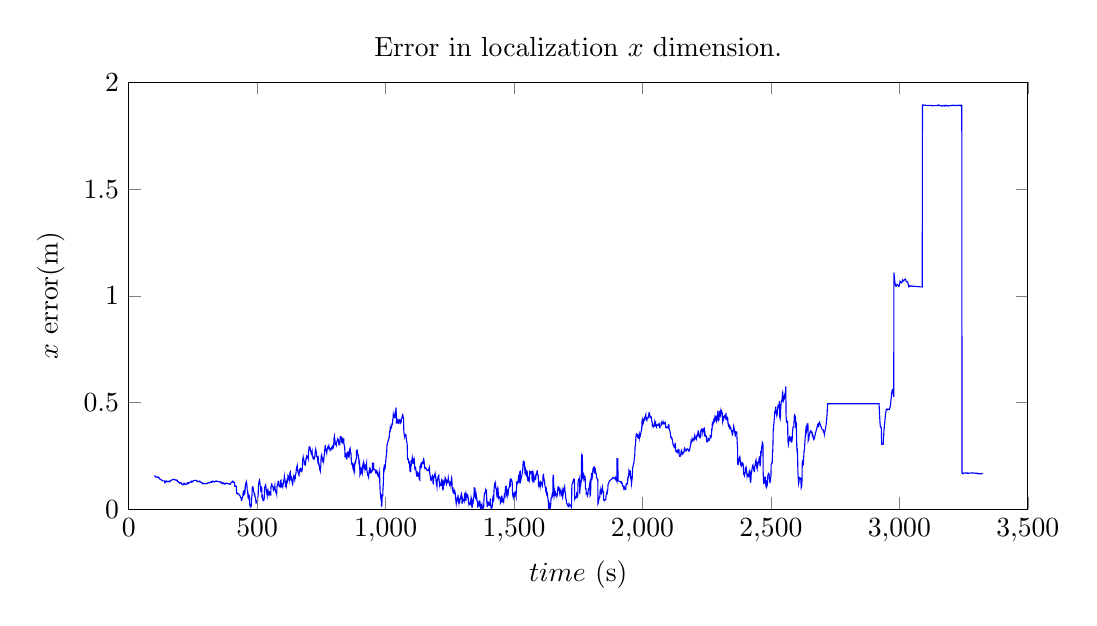
\begin{tikzpicture}

\begin{axis}[
title={Error in localization $x$ dimension.},
xlabel={$time$ (s)},
ylabel={$x$ error(m)},
xmin=0, xmax=3500,
ymin=0, ymax=2,
axis on top,
width=13cm,
height=7cm
]
\addplot [blue]
coordinates {
(100,0.154560091018677)
(101,0.155341627120972)
(102,0.154450180053711)
(103,0.154919626235962)
(104,0.154369356155395)
(105,0.150507843017578)
(106,0.15070096206665)
(107,0.150940811157227)
(108,0.150674839019775)
(109,0.150254030227661)
(110,0.149993677139282)
(111,0.150359649658203)
(112,0.149460399627686)
(113,0.148929441452026)
(114,0.148222291946411)
(115,0.150515342712402)
(116,0.149656320571899)
(117,0.14869549369812)
(118,0.147420431137085)
(119,0.143783067703247)
(120,0.142423128128052)
(121,0.141374086380005)
(122,0.140024160385132)
(123,0.139605974197388)
(124,0.138773178100586)
(125,0.138306354522705)
(126,0.138238903045655)
(127,0.137141939163208)
(128,0.136389013290406)
(129,0.135437582015991)
(130,0.134401414871216)
(131,0.134128902435303)
(132,0.133405063629151)
(133,0.132852256774902)
(134,0.132470310211182)
(135,0.132583559036255)
(136,0.1325556640625)
(137,0.13264864730835)
(138,0.132584512710571)
(139,0.132482707977295)
(140,0.127607400894165)
(141,0.123598392486572)
(142,0.123542840957642)
(143,0.124467428207398)
(144,0.130654996871948)
(145,0.131547159194946)
(146,0.132195896148682)
(147,0.129378456115723)
(148,0.129503387451172)
(149,0.129758018493652)
(150,0.129006284713745)
(151,0.130411346435547)
(152,0.130404670715332)
(153,0.130118806838989)
(154,0.130009134292603)
(155,0.130641897201538)
(156,0.131316860198975)
(157,0.131270606994629)
(158,0.128299819946289)
(159,0.129021274566651)
(160,0.12859164428711)
(161,0.131781272888184)
(162,0.131771974563599)
(163,0.132471733093262)
(164,0.133216552734375)
(165,0.134170135498047)
(166,0.134620985031128)
(167,0.135521730422974)
(168,0.137143930435181)
(169,0.137929996490479)
(170,0.138773759841919)
(171,0.138630470275879)
(172,0.139191707611084)
(173,0.139060815811157)
(174,0.139525016784668)
(175,0.139330228805542)
(176,0.137986074447632)
(177,0.137319456100464)
(178,0.137133728027344)
(179,0.138888580322265)
(180,0.139002067565918)
(181,0.13730834197998)
(182,0.137294275283813)
(183,0.13628528213501)
(184,0.135938383102417)
(185,0.134991384506226)
(186,0.13446471786499)
(187,0.136292381286621)
(188,0.135417146682739)
(189,0.135233564376831)
(190,0.129140506744385)
(191,0.128698240280151)
(192,0.127791772842407)
(193,0.128579553604126)
(194,0.127703603744507)
(195,0.126618322372436)
(196,0.12536209487915)
(197,0.12295574760437)
(198,0.122259088516235)
(199,0.121543117523193)
(200,0.123581651687622)
(201,0.122652296066284)
(202,0.122129682540894)
(203,0.121664289474487)
(204,0.123590978622437)
(205,0.122837337493896)
(206,0.122150215148926)
(207,0.115419687271118)
(208,0.114885629653931)
(209,0.114558996200562)
(210,0.11538487815857)
(211,0.115400150299072)
(212,0.11501868057251)
(213,0.114698961257935)
(214,0.114479377746582)
(215,0.121825611114502)
(216,0.121822988510132)
(217,0.121798908233643)
(218,0.117220575332642)
(219,0.117100889205933)
(220,0.116973812103272)
(221,0.115247587203979)
(222,0.115450242996216)
(223,0.115997175216675)
(224,0.116369585037231)
(225,0.117847576141358)
(226,0.118795766830444)
(227,0.119219913482666)
(228,0.123230152130127)
(229,0.123814277648926)
(230,0.124191455841065)
(231,0.120028310775757)
(232,0.12116580581665)
(233,0.121095472335815)
(234,0.121263557434082)
(235,0.122884948730469)
(236,0.123108823776245)
(237,0.123787839889526)
(238,0.126468000411987)
(239,0.12690788269043)
(240,0.126955089569092)
(241,0.127860126495361)
(242,0.128715572357178)
(243,0.129599151611328)
(244,0.130447444915772)
(245,0.126257329940796)
(246,0.126233011245727)
(247,0.126762538909912)
(248,0.130731292724609)
(249,0.130769201278687)
(250,0.131682821273804)
(251,0.132054515838623)
(252,0.132653661727905)
(253,0.134146877288818)
(254,0.134644218444824)
(255,0.134551712036133)
(256,0.134734817504883)
(257,0.134863563537598)
(258,0.134720750808716)
(259,0.135322217941284)
(260,0.134294872283935)
(261,0.134141807556152)
(262,0.133904581069946)
(263,0.13372576713562)
(264,0.134018306732178)
(265,0.134204034805298)
(266,0.129832418441772)
(267,0.129728706359863)
(268,0.129613073348999)
(269,0.130488990783691)
(270,0.130502342224121)
(271,0.130120157241821)
(272,0.129808305740356)
(273,0.129924980163574)
(274,0.129297939300537)
(275,0.128546443939209)
(276,0.131323884963989)
(277,0.13060195350647)
(278,0.129915307998657)
(279,0.128095945358277)
(280,0.127411684036255)
(281,0.126865467071533)
(282,0.125399473190308)
(283,0.125004652023315)
(284,0.124493482589722)
(285,0.123911741256714)
(286,0.119716255187988)
(287,0.119274942398071)
(288,0.119019119262695)
(289,0.121377067565918)
(290,0.120580749511719)
(291,0.119759159088135)
(292,0.118892877578735)
(293,0.119083135604858)
(294,0.119306533813476)
(295,0.119512050628662)
(296,0.1197991065979)
(297,0.120082109451294)
(298,0.120019166946411)
(299,0.11985125541687)
(300,0.119974517822266)
(301,0.119860792160034)
(302,0.119789028167725)
(303,0.119113430023194)
(304,0.119462236404419)
(305,0.119864686965943)
(306,0.119981273651123)
(307,0.122419048309326)
(308,0.122657466888428)
(309,0.123046804428101)
(310,0.12352721786499)
(311,0.124014068603516)
(312,0.124217916488647)
(313,0.122988483428955)
(314,0.123454591751099)
(315,0.123662731170654)
(316,0.125686153411865)
(317,0.12584684753418)
(318,0.126232608795166)
(319,0.127670372009277)
(320,0.128244483947754)
(321,0.128739679336548)
(322,0.125911623001099)
(323,0.126179128646851)
(324,0.12661710357666)
(325,0.127089649200439)
(326,0.131186176300049)
(327,0.131468702316284)
(328,0.131544757843018)
(329,0.13002710723877)
(330,0.129753164291382)
(331,0.12959962272644)
(332,0.12881427192688)
(333,0.126889699935913)
(334,0.12716388130188)
(335,0.127590650558472)
(336,0.130026836395264)
(337,0.129927892684937)
(338,0.130386610031128)
(339,0.130460996627808)
(340,0.132626285552979)
(341,0.132821073532105)
(342,0.132790079116822)
(343,0.130167324066162)
(344,0.130229551315308)
(345,0.130110580444336)
(346,0.129833776473999)
(347,0.129691440582275)
(348,0.129412729263306)
(349,0.129232961654663)
(350,0.128840047836304)
(351,0.128454286575317)
(352,0.128145534515381)
(353,0.128546522140503)
(354,0.127896354675293)
(355,0.127479122161865)
(356,0.127047107696533)
(357,0.124886922836304)
(358,0.124531202316284)
(359,0.127247882843017)
(360,0.126933647155762)
(361,0.126834941864014)
(362,0.126686168670654)
(363,0.119868267059326)
(364,0.119571674346924)
(365,0.11919854927063)
(366,0.121315784454346)
(367,0.121234722137451)
(368,0.120756931304931)
(369,0.12267985534668)
(370,0.122335102081299)
(371,0.121857549667359)
(372,0.11758020401001)
(373,0.117519645690918)
(374,0.116956977844239)
(375,0.116915254592896)
(376,0.120593076705933)
(377,0.120980745315552)
(378,0.121219640731812)
(379,0.121311908721924)
(380,0.121274953842163)
(381,0.121340280532837)
(382,0.121321207046509)
(383,0.119506313323975)
(384,0.119559957504273)
(385,0.119630529403687)
(386,0.120084955215454)
(387,0.120223394393921)
(388,0.118751636505127)
(389,0.117645374298096)
(390,0.117179618835449)
(391,0.117419944763184)
(392,0.117646919250488)
(393,0.116095582962036)
(394,0.116135160446167)
(395,0.116358797073364)
(396,0.120857564926148)
(397,0.121961919784546)
(398,0.122786848068237)
(399,0.123918382644653)
(400,0.124745218276978)
(401,0.126482574462891)
(402,0.127220003128052)
(403,0.128630725860596)
(404,0.129704086303711)
(405,0.131228773117066)
(406,0.126759582519531)
(407,0.127956443786621)
(408,0.127851062774658)
(409,0.127888494491577)
(410,0.123923425674438)
(411,0.124219779968262)
(412,0.124014978408813)
(413,0.107349143981934)
(414,0.107532487869263)
(415,0.107342468261719)
(416,0.107286201477051)
(417,0.107186304092407)
(418,0.106988893508911)
(419,0.107064233779907)
(420,0.0743128414154053)
(421,0.074164306640625)
(422,0.0745729560852051)
(423,0.0746938343048096)
(424,0.0714864349365234)
(425,0.0712110614776611)
(426,0.0712005710601806)
(427,0.072446975708008)
(428,0.0713376140594484)
(429,0.0704957580566408)
(430,0.0665122299194336)
(431,0.0653127460479737)
(432,0.0645283489227295)
(433,0.0629023342132569)
(434,0.0606707363128662)
(435,0.057348373413086)
(436,0.0532676010131836)
(437,0.053624599456787)
(438,0.0474686317443846)
(439,0.041042058944702)
(440,0.04163885307312)
(441,0.0437738914489745)
(442,0.0538587589263915)
(443,0.0564546604156493)
(444,0.0577145347595214)
(445,0.070049835205078)
(446,0.0815683135986327)
(447,0.0833175182342529)
(448,0.0752387046813965)
(449,0.0684185028076172)
(450,0.0698606967926025)
(451,0.0805112228393554)
(452,0.0763720378875732)
(453,0.0804511413574218)
(454,0.110376234054566)
(455,0.116931791305542)
(456,0.121658439636231)
(457,0.119216419219971)
(458,0.127455926895142)
(459,0.122746921539307)
(460,0.118333316802979)
(461,0.0904057998657226)
(462,0.087136604309082)
(463,0.087202407836914)
(464,0.0587583866119386)
(465,0.0539521064758302)
(466,0.0543440666198731)
(467,0.0592478599548341)
(468,0.0487643089294436)
(469,0.0443523731231692)
(470,0.0495229568481448)
(471,0.0201816692352295)
(472,0.0184416904449463)
(473,0.0130143299102783)
(474,0.0184825096130372)
(475,0.0212283763885499)
(476,0.0207276973724366)
(477,0.017982069015503)
(478,0.0494297752380373)
(479,0.05679571723938)
(480,0.062671543121338)
(481,0.0994164848327639)
(482,0.104033460617066)
(483,0.10555027961731)
(484,0.103146543502808)
(485,0.0932717227935793)
(486,0.0839383506774904)
(487,0.0830678844451906)
(488,0.0758411788940432)
(489,0.0671062374114992)
(490,0.0643627548217776)
(491,0.0667109394073488)
(492,0.0576598949432374)
(493,0.0562548942565919)
(494,0.0538497276306154)
(495,0.0358372745513917)
(496,0.0385244903564455)
(497,0.033340078353882)
(498,0.0377386474609374)
(499,0.0370458030700682)
(500,0.0367606544494627)
(501,0.0319889450073241)
(502,0.0512063732147219)
(503,0.0584242572784426)
(504,0.0666194190979006)
(505,0.112278350830078)
(506,0.116487154006958)
(507,0.129228004455566)
(508,0.133886465072632)
(509,0.136337337493897)
(510,0.128096160888672)
(511,0.122506198883057)
(512,0.106730760574341)
(513,0.0979493274688723)
(514,0.0845468654632571)
(515,0.0833840980529788)
(516,0.102090433120728)
(517,0.103150918960571)
(518,0.0995691566467287)
(519,0.0527169361114503)
(520,0.0619609012603761)
(521,0.0626816406250001)
(522,0.0441071662902832)
(523,0.040115800857544)
(524,0.0412349376678467)
(525,0.0402373943328858)
(526,0.0400292243957519)
(527,0.047259983062744)
(528,0.0562452640533446)
(529,0.0989891262054443)
(530,0.103898880004883)
(531,0.107973930358887)
(532,0.11054455947876)
(533,0.113231309890747)
(534,0.103915580749512)
(535,0.0964235153198243)
(536,0.0832542495727537)
(537,0.0813869552612303)
(538,0.0703438835144041)
(539,0.0636850910186766)
(540,0.0844815540313721)
(541,0.0880773830413819)
(542,0.0905972290039063)
(543,0.067362787246704)
(544,0.0668849964141844)
(545,0.0731749553680419)
(546,0.0682985801696776)
(547,0.0738872737884524)
(548,0.0689908714294436)
(549,0.0684088916778567)
(550,0.0752517280578613)
(551,0.0715107021331787)
(552,0.0756653842926025)
(553,0.0727454719543457)
(554,0.10622470664978)
(555,0.108473470687866)
(556,0.117788722991943)
(557,0.11702607345581)
(558,0.112180931091308)
(559,0.108561975479126)
(560,0.104930601119995)
(561,0.104451141357422)
(562,0.104191265106201)
(563,0.0902215538024902)
(564,0.0879141387939453)
(565,0.09011545753479)
(566,0.10186067199707)
(567,0.101439754486084)
(568,0.101482192993164)
(569,0.110163251876831)
(570,0.0938412475585939)
(571,0.0888973999023439)
(572,0.0792896080017091)
(573,0.0778374004364015)
(574,0.0821730060577393)
(575,0.0800610942840576)
(576,0.0729688568115234)
(577,0.101870517730713)
(578,0.106464605331421)
(579,0.114819269180298)
(580,0.11420557975769)
(581,0.124962434768677)
(582,0.130569086074829)
(583,0.129585847854614)
(584,0.1211243724823)
(585,0.109287515640259)
(586,0.107616678237915)
(587,0.107391134262085)
(588,0.107275735855103)
(589,0.104391586303711)
(590,0.108723651885986)
(591,0.13258207321167)
(592,0.133970623016357)
(593,0.135296945571899)
(594,0.112417106628418)
(595,0.115561609268188)
(596,0.11261284828186)
(597,0.106796388626099)
(598,0.109919002532959)
(599,0.114531209945679)
(600,0.108121803283691)
(601,0.116766351699829)
(602,0.120619672775268)
(603,0.127392190933227)
(604,0.137044868469238)
(605,0.139126262664795)
(606,0.153593263626099)
(607,0.145079040527344)
(608,0.139726781845093)
(609,0.134060764312744)
(610,0.109356582641602)
(611,0.110448301315308)
(612,0.105173051834107)
(613,0.102568328857422)
(614,0.123013362884521)
(615,0.129007444381714)
(616,0.133467063903808)
(617,0.125375705718994)
(618,0.128333526611328)
(619,0.134300428390503)
(620,0.157348594665527)
(621,0.155487499237061)
(622,0.147109470367432)
(623,0.152723596572876)
(624,0.152924345016479)
(625,0.146118925094604)
(626,0.139171407699585)
(627,0.164499177932739)
(628,0.171442880630493)
(629,0.173817529678345)
(630,0.149746850967407)
(631,0.154025987625122)
(632,0.154091075897217)
(633,0.147271589279175)
(634,0.136686553955078)
(635,0.132488956451416)
(636,0.129664649963379)
(637,0.118466529846192)
(638,0.115446243286133)
(639,0.120937976837158)
(640,0.147473203659058)
(641,0.149927484512329)
(642,0.148987161636353)
(643,0.156073677062988)
(644,0.152492540359497)
(645,0.145107524871826)
(646,0.138808744430542)
(647,0.152468074798584)
(648,0.155781377792358)
(649,0.15252219581604)
(650,0.164763673782349)
(651,0.166317686080933)
(652,0.17953394317627)
(653,0.192531332015991)
(654,0.196205219268799)
(655,0.201659759521485)
(656,0.205657085418701)
(657,0.187072591781616)
(658,0.181186037063599)
(659,0.173858480453491)
(660,0.172316621780396)
(661,0.168789934158325)
(662,0.161352466583252)
(663,0.158851694107056)
(664,0.17516224861145)
(665,0.184626035690308)
(666,0.187051944732666)
(667,0.18078076171875)
(668,0.186708086013794)
(669,0.190601222991944)
(670,0.189130083084106)
(671,0.182164445877075)
(672,0.177389636993408)
(673,0.179271951675415)
(674,0.181368974685669)
(675,0.18054333114624)
(676,0.195112613677979)
(677,0.225720401763916)
(678,0.236631866455078)
(679,0.244339700698853)
(680,0.235571439743042)
(681,0.235798652648926)
(682,0.229530866622925)
(683,0.224749858856201)
(684,0.213423908233643)
(685,0.214611709594727)
(686,0.208978116989136)
(687,0.206923820495605)
(688,0.210508205413818)
(689,0.221402265548706)
(690,0.235731224060059)
(691,0.234664539337158)
(692,0.240339378356934)
(693,0.248040386199951)
(694,0.245377012252808)
(695,0.240751453399658)
(696,0.240272947311401)
(697,0.248315418243408)
(698,0.248024785995483)
(699,0.241157377243042)
(700,0.271371189117432)
(701,0.275184217453003)
(702,0.289880100250244)
(703,0.290506425857544)
(704,0.287301147460937)
(705,0.290919626235962)
(706,0.287233913421631)
(707,0.279338659286499)
(708,0.271219791412354)
(709,0.271975816726685)
(710,0.266223253250122)
(711,0.258176387786865)
(712,0.256902040481568)
(713,0.26231223487854)
(714,0.268802942276001)
(715,0.249102653503418)
(716,0.249502004623413)
(717,0.241062101364136)
(718,0.241643127441406)
(719,0.236449893951416)
(720,0.238554138183594)
(721,0.238443035125732)
(722,0.236893314361572)
(723,0.24402117729187)
(724,0.243102550506592)
(725,0.249974489212036)
(726,0.274371408462525)
(727,0.275846981048584)
(728,0.28187467956543)
(729,0.27328483581543)
(730,0.269512815475464)
(731,0.264745874404907)
(732,0.247580923080444)
(733,0.246768392562866)
(734,0.241749443054199)
(735,0.233699478149414)
(736,0.248255411148071)
(737,0.229741970062256)
(738,0.235230604171753)
(739,0.217919523239136)
(740,0.208926612854004)
(741,0.210521156311035)
(742,0.203548784255982)
(743,0.190247173309326)
(744,0.185353155136109)
(745,0.187092657089234)
(746,0.18069803237915)
(747,0.194668407440186)
(748,0.204091901779175)
(749,0.246644472122192)
(750,0.249756788253784)
(751,0.253830884933472)
(752,0.243805221557617)
(753,0.244099668502808)
(754,0.239139608383179)
(755,0.230698637008667)
(756,0.236846809387207)
(757,0.236388330459595)
(758,0.232056741714477)
(759,0.224845294952392)
(760,0.238717203140259)
(761,0.252699022293091)
(762,0.256352310180664)
(763,0.279394115447998)
(764,0.28407212638855)
(765,0.299510444641113)
(766,0.288110118865967)
(767,0.277736526489258)
(768,0.274345975875855)
(769,0.276310068130493)
(770,0.27310524559021)
(771,0.264577489852905)
(772,0.27386675453186)
(773,0.283477169036865)
(774,0.286406618118286)
(775,0.289896827697754)
(776,0.295672756195068)
(777,0.296269994735718)
(778,0.289758544921875)
(779,0.295508703231812)
(780,0.288443407058716)
(781,0.288824638366699)
(782,0.285798694610596)
(783,0.281901266098023)
(784,0.275876190185547)
(785,0.27802767944336)
(786,0.283360864639282)
(787,0.283792163848877)
(788,0.284208442687989)
(789,0.287251161575317)
(790,0.288737224578858)
(791,0.28323547744751)
(792,0.289417909622192)
(793,0.296789182662964)
(794,0.296915306091309)
(795,0.289855016708374)
(796,0.286715282440186)
(797,0.289926542282104)
(798,0.295393241882324)
(799,0.332272741317749)
(800,0.33409568977356)
(801,0.340956661224365)
(802,0.328126607894898)
(803,0.321905075073242)
(804,0.309971748352051)
(805,0.303494153976441)
(806,0.303529678344727)
(807,0.300895629882813)
(808,0.29834359741211)
(809,0.310916604995727)
(810,0.314475002288818)
(811,0.318555536270142)
(812,0.321468746185303)
(813,0.326074039459229)
(814,0.330123579025269)
(815,0.32701317024231)
(816,0.325410018920898)
(817,0.316511283874512)
(818,0.307715545654297)
(819,0.310495267868042)
(820,0.310161720275879)
(821,0.301942478179932)
(822,0.30161918258667)
(823,0.336648248672486)
(824,0.339581512451172)
(825,0.339783452987671)
(826,0.336281661987305)
(827,0.337488298416138)
(828,0.33287299156189)
(829,0.320972328186035)
(830,0.311473970413208)
(831,0.310175542831421)
(832,0.309772615432739)
(833,0.325458377838135)
(834,0.321312755584717)
(835,0.324962944030762)
(836,0.329352945327759)
(837,0.329585403442383)
(838,0.303546041488648)
(839,0.299121946334839)
(840,0.294333005905151)
(841,0.287802482604981)
(842,0.242436672210693)
(843,0.254259031295776)
(844,0.254838626861572)
(845,0.251581113815308)
(846,0.265100599288941)
(847,0.253166080474854)
(848,0.232114912033081)
(849,0.243746671676636)
(850,0.242489490509033)
(851,0.252945337295532)
(852,0.254483613967896)
(853,0.270942987442017)
(854,0.260166706085205)
(855,0.254070104598999)
(856,0.258871793746948)
(857,0.259587049484253)
(858,0.240131378173828)
(859,0.273912662506103)
(860,0.278962844848633)
(861,0.284364456176758)
(862,0.286747211456299)
(863,0.2641097240448)
(864,0.264648788452149)
(865,0.264571302413941)
(866,0.242704946517944)
(867,0.218247491836548)
(868,0.213686544418335)
(869,0.216962177276611)
(870,0.214002687454224)
(871,0.209884244918823)
(872,0.200440246582031)
(873,0.206751735687256)
(874,0.203668268203736)
(875,0.193563135147095)
(876,0.199923666000366)
(877,0.181604162216186)
(878,0.185591474533081)
(879,0.178755537033081)
(880,0.210899457931518)
(881,0.212545499801636)
(882,0.220921621322632)
(883,0.219157562255859)
(884,0.222785339355469)
(885,0.233668193817139)
(886,0.239607915878296)
(887,0.273992893218994)
(888,0.275468227386475)
(889,0.276652214050293)
(890,0.272273529052734)
(891,0.265959728240967)
(892,0.254338014602661)
(893,0.247127521514892)
(894,0.248950946807861)
(895,0.240269887924194)
(896,0.231341112136841)
(897,0.204780109405517)
(898,0.21286536026001)
(899,0.216854341506958)
(900,0.164837335586548)
(901,0.169959758758545)
(902,0.167746280670166)
(903,0.196062145233154)
(904,0.185648736953735)
(905,0.178653535842896)
(906,0.183019933700562)
(907,0.176951225280762)
(908,0.170319612503052)
(909,0.166846569061279)
(910,0.200501846313477)
(911,0.205424951553345)
(912,0.209182905197144)
(913,0.215335773468018)
(914,0.196303176879883)
(915,0.195956516265869)
(916,0.189629364013672)
(917,0.205287860870361)
(918,0.198553966522217)
(919,0.200886415481567)
(920,0.203072713851929)
(921,0.195243286132813)
(922,0.189750122070313)
(923,0.194868492126465)
(924,0.206223562240601)
(925,0.208667114257813)
(926,0.215733364105225)
(927,0.177884408950806)
(928,0.177690574645996)
(929,0.169846364974976)
(930,0.158991167068482)
(931,0.158967880249024)
(932,0.158795742034912)
(933,0.153901723861694)
(934,0.149433759689331)
(935,0.171088344573975)
(936,0.177908784866333)
(937,0.185877449035645)
(938,0.18007586479187)
(939,0.174956064224243)
(940,0.177550535202026)
(941,0.182594757080078)
(942,0.171109132766724)
(943,0.171885423660278)
(944,0.171420984268189)
(945,0.178561014175415)
(946,0.178289693832398)
(947,0.178044361114502)
(948,0.178935092926026)
(949,0.21285401725769)
(950,0.211477149963379)
(951,0.212569822311401)
(952,0.213293661117554)
(953,0.214655031204224)
(954,0.18513251876831)
(955,0.185000434875488)
(956,0.184654251098633)
(957,0.185039953231811)
(958,0.184277729034424)
(959,0.18411417388916)
(960,0.183927015304565)
(961,0.170142223358154)
(962,0.169714023590088)
(963,0.169171859741211)
(964,0.180830289840698)
(965,0.179608633041382)
(966,0.178908159255982)
(967,0.177055170059204)
(968,0.163384674072266)
(969,0.161349771499634)
(970,0.157839057922363)
(971,0.158813419342041)
(972,0.15520209312439)
(973,0.158606948852539)
(974,0.166726959228516)
(975,0.173606527328491)
(976,0.147001159667969)
(977,0.153399122238159)
(978,0.109580457687378)
(979,0.0765296821594239)
(980,0.0716385250091554)
(981,0.0533713035583498)
(982,0.0539253883361819)
(983,0.0500482254028323)
(984,0.0120800800323484)
(985,0.0450018577575682)
(986,0.0378202133178709)
(987,0.0634525947570799)
(988,0.0609164218902589)
(989,0.0640728454589845)
(990,0.100223062515259)
(991,0.115984199523926)
(992,0.146503030776977)
(993,0.189941942214966)
(994,0.196789800643921)
(995,0.186454355239868)
(996,0.19339328956604)
(997,0.188101589202881)
(998,0.189190923690796)
(999,0.206949054718017)
(1000,0.212074815750122)
(1001,0.233857069015503)
(1002,0.243041429519653)
(1003,0.250847730636597)
(1004,0.259600477218628)
(1005,0.288831787109375)
(1006,0.302903490066528)
(1007,0.305063323974609)
(1008,0.312856750488281)
(1009,0.318072395324707)
(1010,0.319473104476929)
(1011,0.322809022903442)
(1012,0.327619117736816)
(1013,0.332929891586303)
(1014,0.33351997756958)
(1015,0.354768602371216)
(1016,0.363323776245117)
(1017,0.367352096557617)
(1018,0.380129663467407)
(1019,0.371565191268921)
(1020,0.375573722839355)
(1021,0.381189195632934)
(1022,0.380543796539306)
(1023,0.382343379974365)
(1024,0.393793909072876)
(1025,0.399252740859985)
(1026,0.398252574920654)
(1027,0.402146427154541)
(1028,0.420022336959839)
(1029,0.427082626342773)
(1030,0.44399031829834)
(1031,0.436946479797363)
(1032,0.438273040771484)
(1033,0.43546113204956)
(1034,0.430812923431396)
(1035,0.429584352493286)
(1036,0.444460956573486)
(1037,0.450903980255127)
(1038,0.444497196197509)
(1039,0.439589111328125)
(1040,0.467087356567383)
(1041,0.476361600875854)
(1042,0.401455297470093)
(1043,0.409583702087402)
(1044,0.408108606338501)
(1045,0.411682024002075)
(1046,0.407433179855347)
(1047,0.406366971969605)
(1048,0.41474070930481)
(1049,0.404563869476319)
(1050,0.405302490234375)
(1051,0.402559484481812)
(1052,0.401759351730347)
(1053,0.411619867324829)
(1054,0.419620241165161)
(1055,0.419497932434082)
(1056,0.417857612609863)
(1057,0.415092910766602)
(1058,0.410004819869995)
(1059,0.403969491958618)
(1060,0.405663932800293)
(1061,0.415483678817749)
(1062,0.42447945022583)
(1063,0.427912439346314)
(1064,0.427828039169312)
(1065,0.435795272827149)
(1066,0.444046939849854)
(1067,0.443099941253662)
(1068,0.436303104400635)
(1069,0.426906551361084)
(1070,0.424752439498902)
(1071,0.362608995437622)
(1072,0.355453338623047)
(1073,0.349895086288452)
(1074,0.3403141040802)
(1075,0.345696880340576)
(1076,0.344736530303955)
(1077,0.344963266372681)
(1078,0.349732353210449)
(1079,0.348901226043701)
(1080,0.337271167755127)
(1081,0.326142980575562)
(1082,0.317184879302979)
(1083,0.311706020355225)
(1084,0.307130767822266)
(1085,0.243885580062866)
(1086,0.235401454925537)
(1087,0.236796203613281)
(1088,0.234846893310547)
(1089,0.230138126373291)
(1090,0.220985237121582)
(1091,0.223223033905029)
(1092,0.221973720550537)
(1093,0.209598604202271)
(1094,0.197175804138184)
(1095,0.179726663589478)
(1096,0.175798717498779)
(1097,0.17640096282959)
(1098,0.179337087631226)
(1099,0.225029983520508)
(1100,0.224788942337036)
(1101,0.218609132766724)
(1102,0.230048114776611)
(1103,0.231892997741699)
(1104,0.242114240646362)
(1105,0.235000783920288)
(1106,0.222131029129028)
(1107,0.215020433425903)
(1108,0.215165153503418)
(1109,0.217667356491089)
(1110,0.233041706085205)
(1111,0.236843528747559)
(1112,0.230355205535889)
(1113,0.198175971984863)
(1114,0.188245361328125)
(1115,0.189591472625732)
(1116,0.19230419921875)
(1117,0.194220230102539)
(1118,0.182816669464111)
(1119,0.177065774917602)
(1120,0.16119567489624)
(1121,0.15853659248352)
(1122,0.154368558883667)
(1123,0.153998294830322)
(1124,0.170843137741089)
(1125,0.168557180404663)
(1126,0.157150997161865)
(1127,0.158306991577148)
(1128,0.161184703826904)
(1129,0.164646780014038)
(1130,0.151836311340332)
(1131,0.142871295928955)
(1132,0.13856044960022)
(1133,0.136912261962891)
(1134,0.200152574539184)
(1135,0.200572668075561)
(1136,0.204947172164917)
(1137,0.194582639694214)
(1138,0.195517955780029)
(1139,0.194444595336914)
(1140,0.194702325820923)
(1141,0.218602886199951)
(1142,0.219049444198608)
(1143,0.219048490524292)
(1144,0.221075923919678)
(1145,0.220967205047607)
(1146,0.221744449615478)
(1147,0.212074192047119)
(1148,0.240173391342163)
(1149,0.232096485137939)
(1150,0.224707178115845)
(1151,0.198964241027832)
(1152,0.195873620986939)
(1153,0.19174135017395)
(1154,0.195573076248169)
(1155,0.193127378463745)
(1156,0.192810520172119)
(1157,0.190935949325561)
(1158,0.18990669631958)
(1159,0.189618686676025)
(1160,0.188942770004272)
(1161,0.181745124816894)
(1162,0.181412769317627)
(1163,0.181020332336426)
(1164,0.180364603042602)
(1165,0.180073017120361)
(1166,0.179920190811157)
(1167,0.181387657165527)
(1168,0.187085220336914)
(1169,0.191031763076782)
(1170,0.195494482040405)
(1171,0.181751174926758)
(1172,0.167835874557495)
(1173,0.16014949798584)
(1174,0.15085816192627)
(1175,0.146526573181152)
(1176,0.135518310546875)
(1177,0.13406014251709)
(1178,0.135438089370727)
(1179,0.144312267303467)
(1180,0.144646291732788)
(1181,0.153403564453125)
(1182,0.156400485992432)
(1183,0.149852558135986)
(1184,0.136684135437012)
(1185,0.12090034866333)
(1186,0.11961074256897)
(1187,0.155679590225219)
(1188,0.147733814239502)
(1189,0.153827554702759)
(1190,0.157429607391357)
(1191,0.161379487991333)
(1192,0.157358081817627)
(1193,0.16517511177063)
(1194,0.157361881256104)
(1195,0.153822557449341)
(1196,0.13954319190979)
(1197,0.123589532852173)
(1198,0.116811531066895)
(1199,0.112860935211182)
(1200,0.105828540802002)
(1201,0.134769968032837)
(1202,0.138329557418823)
(1203,0.143313459396362)
(1204,0.150109914779663)
(1205,0.152396348953247)
(1206,0.156742719650269)
(1207,0.158457426071167)
(1208,0.135415985107422)
(1209,0.124983980178833)
(1210,0.115029766082764)
(1211,0.122856616973877)
(1212,0.118738412857056)
(1213,0.110637903213501)
(1214,0.111225584030151)
(1215,0.112002590179443)
(1216,0.117936590194702)
(1217,0.119330862045288)
(1218,0.131830890655518)
(1219,0.137801607131958)
(1220,0.134738405227661)
(1221,0.101381576538086)
(1222,0.0944743518829347)
(1223,0.0905862216949465)
(1224,0.0903647308349611)
(1225,0.11734356880188)
(1226,0.110754871368408)
(1227,0.112004661560059)
(1228,0.113143825531006)
(1229,0.13104033279419)
(1230,0.129442213058472)
(1231,0.132854221343994)
(1232,0.147702470779419)
(1233,0.145486608505249)
(1234,0.140789762496948)
(1235,0.125893697738647)
(1236,0.122053489685058)
(1237,0.11794506072998)
(1238,0.128163270950318)
(1239,0.123782806396485)
(1240,0.123852663040161)
(1241,0.127628736495972)
(1242,0.134528331756592)
(1243,0.133795194625855)
(1244,0.145390682220459)
(1245,0.135793954849243)
(1246,0.131739646911621)
(1247,0.123454839706421)
(1248,0.118773490905762)
(1249,0.122918087005615)
(1250,0.120184379577637)
(1251,0.113442140579223)
(1252,0.125880670547485)
(1253,0.127457571029663)
(1254,0.12798376083374)
(1255,0.123014879226684)
(1256,0.139492366790771)
(1257,0.147041414260864)
(1258,0.140922878265381)
(1259,0.10401634979248)
(1260,0.0948212604522705)
(1261,0.0893571834564209)
(1262,0.102750162124634)
(1263,0.0905905761718748)
(1264,0.0796218910217283)
(1265,0.0771666564941405)
(1266,0.0814660205841062)
(1267,0.0808251514434812)
(1268,0.0770805492401121)
(1269,0.0853453483581541)
(1270,0.0812807884216307)
(1271,0.0753818359374998)
(1272,0.0567734470367429)
(1273,0.0470433464050291)
(1274,0.0347936382293699)
(1275,0.0254876842498777)
(1276,0.0344517154693604)
(1277,0.0343248767852784)
(1278,0.034884922027588)
(1279,0.0527060852050782)
(1280,0.0519882068634034)
(1281,0.0566862449645997)
(1282,0.0660704002380372)
(1283,0.0485048866271973)
(1284,0.0385468578338624)
(1285,0.0310729122161866)
(1286,0.0481101303100586)
(1287,0.0483661918640137)
(1288,0.0429939060211182)
(1289,0.0377775459289551)
(1290,0.0473433265686034)
(1291,0.0507255325317382)
(1292,0.0534697303771972)
(1293,0.0607469501495359)
(1294,0.0665898742675779)
(1295,0.0727012577056882)
(1296,0.0685842456817625)
(1297,0.0375641345977784)
(1298,0.027931308746338)
(1299,0.0282393455505372)
(1300,0.0476358070373535)
(1301,0.0433814659118652)
(1302,0.0407655372619629)
(1303,0.0395655765533447)
(1304,0.0388511676788328)
(1305,0.0413326282501219)
(1306,0.0377484817504881)
(1307,0.0636640892028808)
(1308,0.0719622478485107)
(1309,0.0742882595062255)
(1310,0.0639613971710205)
(1311,0.0408102741241456)
(1312,0.040264295578003)
(1313,0.0428311100006105)
(1314,0.0677310218811034)
(1315,0.0618273010253905)
(1316,0.0598112335205077)
(1317,0.0578814735412596)
(1318,0.0622023391723632)
(1319,0.0584803867340087)
(1320,0.0622760105133056)
(1321,0.0573023948669431)
(1322,0.0458754692077634)
(1323,0.0313743743896482)
(1324,0.0241276416778562)
(1325,0.0294603576660157)
(1326,0.0283502807617189)
(1327,0.0248507728576661)
(1328,0.0219742622375487)
(1329,0.0212923851013183)
(1330,0.0266680088043212)
(1331,0.0377868480682371)
(1332,0.0447911090850828)
(1333,0.053935176849365)
(1334,0.0479577846527097)
(1335,0.0240432624816895)
(1336,0.00870245742797859)
(1337,0.00830048370361336)
(1338,0.0306868686676025)
(1339,0.0243351593017578)
(1340,0.0247635974884033)
(1341,0.0368373470306396)
(1342,0.0468020515441894)
(1343,0.0538394527435302)
(1344,0.0634276943206786)
(1345,0.0997243518829345)
(1346,0.0989206428527831)
(1347,0.0789740676879882)
(1348,0.0695963497161864)
(1349,0.0587723789215087)
(1350,0.0581119594573973)
(1351,0.046157651901245)
(1352,0.072589756011963)
(1353,0.0649567852020265)
(1354,0.0577255496978761)
(1355,0.0514215049743654)
(1356,0.0379930553436281)
(1357,0.036382537841797)
(1358,0.0291060028076173)
(1359,0.00727546691894521)
(1360,0.0190080451965331)
(1361,0.0228158283233642)
(1362,0.0232237625122069)
(1363,0.0208242588043213)
(1364,0.0382121257781982)
(1365,0.0383175067901611)
(1366,0.034207250595093)
(1367,0.0352469940185549)
(1368,0.0307828445434573)
(1369,0.00317914009094222)
(1370,0.00572759628295882)
(1371,0.00412886619567887)
(1372,0.0169674682617189)
(1373,0.0209169864654544)
(1374,0.0206642627716067)
(1375,0.0235317230224612)
(1376,0.00441382598876938)
(1377,0.000652091979980618)
(1378,0.000551921844482273)
(1379,0.00131009292602524)
(1380,0.00832508087158201)
(1381,0.0112705039978027)
(1382,0.0109851169586181)
(1383,0.0455589389801028)
(1384,0.0619206523895266)
(1385,0.0749518966674807)
(1386,0.0763449764251711)
(1387,0.0741889533996583)
(1388,0.0793521461486817)
(1389,0.0866377410888672)
(1390,0.0795405349731446)
(1391,0.0799870929718018)
(1392,0.0784435710906983)
(1393,0.0819371185302735)
(1394,0.0339107456207275)
(1395,0.0245332660675048)
(1396,0.010251516342163)
(1397,0.0225016574859618)
(1398,0.0315651397705077)
(1399,0.0333458881378172)
(1400,0.0309550266265868)
(1401,0.0247768001556397)
(1402,0.0205699043273926)
(1403,0.0214613513946533)
(1404,0.019911153793335)
(1405,0.0274110107421874)
(1406,0.0267153053283691)
(1407,0.0302150516510009)
(1408,0.0506716232299804)
(1409,0.0195889930725097)
(1410,0.0101285438537597)
(1411,0.00610084724426274)
(1412,0.01415726852417)
(1413,0.0125128955841065)
(1414,0.00872275543212897)
(1415,0.0136238441467285)
(1416,0.0176798210144042)
(1417,0.0417972908020019)
(1418,0.0346587295532226)
(1419,0.0367127056121825)
(1420,0.0553730125427245)
(1421,0.0516865844726562)
(1422,0.0893278884887696)
(1423,0.103043155670166)
(1424,0.11269624710083)
(1425,0.106620918273926)
(1426,0.106684337615967)
(1427,0.111175905227661)
(1428,0.117714057922363)
(1429,0.0977247180938723)
(1430,0.0965242805480959)
(1431,0.095982116699219)
(1432,0.071208122253418)
(1433,0.0670541553497315)
(1434,0.0577229290008545)
(1435,0.059378984451294)
(1436,0.0898800888061522)
(1437,0.0994404354095457)
(1438,0.0959073104858397)
(1439,0.0519807815551756)
(1440,0.0547104358673094)
(1441,0.0596482038497923)
(1442,0.0596130371093748)
(1443,0.053610849380493)
(1444,0.0527871131896971)
(1445,0.0527823448181151)
(1446,0.0444839477539061)
(1447,0.0292777500152588)
(1448,0.0324494323730469)
(1449,0.0405306301116943)
(1450,0.0547605724334717)
(1451,0.0589855880737304)
(1452,0.0575023860931396)
(1453,0.0587675542831421)
(1454,0.0379022750854494)
(1455,0.0401304159164431)
(1456,0.0406293067932131)
(1457,0.0380622949600222)
(1458,0.0471319761276248)
(1459,0.0467120018005374)
(1460,0.0392107572555545)
(1461,0.0493612213134766)
(1462,0.0632036848068238)
(1463,0.0744558496475221)
(1464,0.0581590461730959)
(1465,0.0574977922439577)
(1466,0.0891892242431642)
(1467,0.104647092819214)
(1468,0.106987626075745)
(1469,0.107612998008728)
(1470,0.101191908836365)
(1471,0.0699154672622682)
(1472,0.0644522247314454)
(1473,0.0598890123367311)
(1474,0.0727476453781128)
(1475,0.0832139825820923)
(1476,0.0933970785140992)
(1477,0.0937908267974854)
(1478,0.0821439361572267)
(1479,0.0934545135498048)
(1480,0.0995190477371217)
(1481,0.102791871070862)
(1482,0.107645000457764)
(1483,0.118045176506043)
(1484,0.105085815429688)
(1485,0.105961765289307)
(1486,0.12617143535614)
(1487,0.140401209831238)
(1488,0.141947354316712)
(1489,0.140263523101807)
(1490,0.135045962333679)
(1491,0.13351734161377)
(1492,0.12993212223053)
(1493,0.121730642318726)
(1494,0.0801844854354858)
(1495,0.0666358728408813)
(1496,0.0595178861618042)
(1497,0.054629288673401)
(1498,0.0647328720092775)
(1499,0.0773130283355714)
(1500,0.0571833534240722)
(1501,0.0584203882217407)
(1502,0.0644206686019897)
(1503,0.0765363149642946)
(1504,0.0797379188537599)
(1505,0.0773850851058961)
(1506,0.0639545326232911)
(1507,0.0627701883316041)
(1508,0.0573444967269898)
(1509,0.0933157682418824)
(1510,0.111483144760132)
(1511,0.130992102622986)
(1512,0.11766276550293)
(1513,0.121489026069641)
(1514,0.126959778785706)
(1515,0.12947175693512)
(1516,0.130330853462219)
(1517,0.14421754360199)
(1518,0.160733871459961)
(1519,0.130056938171387)
(1520,0.12263639831543)
(1521,0.160147031784058)
(1522,0.169371190071106)
(1523,0.176516714096069)
(1524,0.177818121910095)
(1525,0.128461815834045)
(1526,0.131569959640503)
(1527,0.141982175827026)
(1528,0.145698287010193)
(1529,0.15329306602478)
(1530,0.154810361862183)
(1531,0.161045722961426)
(1532,0.170950960159302)
(1533,0.175312708854675)
(1534,0.189831565856934)
(1535,0.21199889087677)
(1536,0.224706112861633)
(1537,0.224536954879761)
(1538,0.224082409858704)
(1539,0.212901103973389)
(1540,0.220709789276123)
(1541,0.220489728927612)
(1542,0.178877961158753)
(1543,0.183573495864868)
(1544,0.187473189353943)
(1545,0.176283490180969)
(1546,0.15872071647644)
(1547,0.172914012908935)
(1548,0.185551866531372)
(1549,0.157521540641785)
(1550,0.152656132698059)
(1551,0.152282292366028)
(1552,0.160303050994873)
(1553,0.140731984138489)
(1554,0.143288427352905)
(1555,0.144989663124085)
(1556,0.137754812240601)
(1557,0.140459909439087)
(1558,0.134401216506958)
(1559,0.131690516471863)
(1560,0.157679594993591)
(1561,0.174831308364868)
(1562,0.172570146560669)
(1563,0.165952916145325)
(1564,0.168483729362488)
(1565,0.174120779037476)
(1566,0.175304433822632)
(1567,0.174945852279663)
(1568,0.175122162818909)
(1569,0.17515113067627)
(1570,0.140473381996155)
(1571,0.134398476600647)
(1572,0.141020433425903)
(1573,0.161358697891235)
(1574,0.17125581073761)
(1575,0.164427979469299)
(1576,0.164741380691528)
(1577,0.125085524559021)
(1578,0.132591895103455)
(1579,0.143907956123352)
(1580,0.144562534332275)
(1581,0.143330176353455)
(1582,0.149786551475525)
(1583,0.145196397781372)
(1584,0.14240558719635)
(1585,0.150889235496521)
(1586,0.1630805311203)
(1587,0.166070180892944)
(1588,0.170159065246582)
(1589,0.171410047531128)
(1590,0.182380997657776)
(1591,0.163232739448547)
(1592,0.163722570419311)
(1593,0.159090335845947)
(1594,0.158958967208862)
(1595,0.121987556457519)
(1596,0.111782406806946)
(1597,0.106082414627075)
(1598,0.108340623855591)
(1599,0.119546535491943)
(1600,0.124161961555481)
(1601,0.120426776885986)
(1602,0.107549188613892)
(1603,0.116807578086853)
(1604,0.124809859275818)
(1605,0.12112434387207)
(1606,0.122901992797852)
(1607,0.1245876121521)
(1608,0.122451977729797)
(1609,0.111496232032776)
(1610,0.108230612754822)
(1611,0.117164991378784)
(1612,0.128341339111328)
(1613,0.158602721214294)
(1614,0.159197337150574)
(1615,0.1612231798172)
(1616,0.138122674942017)
(1617,0.139330741882324)
(1618,0.132640597343445)
(1619,0.130115029335022)
(1620,0.11060923576355)
(1621,0.105915131568909)
(1622,0.100112738609314)
(1623,0.0972585105895996)
(1624,0.0773015203475953)
(1625,0.0899862232208253)
(1626,0.0932980957031251)
(1627,0.0699677782058716)
(1628,0.0717757062911988)
(1629,0.0767546014785767)
(1630,0.0725817995071412)
(1631,0.056163459777832)
(1632,0.0484122333526611)
(1633,0.0419005451202392)
(1634,0.0174743013381957)
(1635,0.00675714778900138)
(1636,0.00106620025634774)
(1637,0.0032659845352172)
(1638,0.0223238143920899)
(1639,0.018048134803772)
(1640,0.0177156600952149)
(1641,0.00674839019775386)
(1642,0.01239914894104)
(1643,0.025639009475708)
(1644,0.0447295427322387)
(1645,0.0525429182052612)
(1646,0.0547270708084107)
(1647,0.0574808053970337)
(1648,0.065698974609375)
(1649,0.073755802154541)
(1650,0.0724019422531128)
(1651,0.0663612499237061)
(1652,0.158274343490601)
(1653,0.157616785049439)
(1654,0.151995113372803)
(1655,0.061166838645935)
(1656,0.0681349792480468)
(1657,0.0814791479110717)
(1658,0.0854771890640258)
(1659,0.0699014654159547)
(1660,0.078589319229126)
(1661,0.079570411682129)
(1662,0.0686368818283081)
(1663,0.0716289157867431)
(1664,0.0692491407394409)
(1665,0.0696630353927612)
(1666,0.0699713621139526)
(1667,0.0601433906555175)
(1668,0.0653125438690185)
(1669,0.0809883270263672)
(1670,0.0918963251113891)
(1671,0.104184537887573)
(1672,0.104442268371582)
(1673,0.0891253356933595)
(1674,0.0878795986175538)
(1675,0.0937743787765504)
(1676,0.10173565196991)
(1677,0.0768687200546265)
(1678,0.0822796297073365)
(1679,0.0825346183776856)
(1680,0.0801408891677857)
(1681,0.0834097270965577)
(1682,0.0883242492675782)
(1683,0.0675618829727171)
(1684,0.0705572547912596)
(1685,0.0733592691421507)
(1686,0.0769249382019042)
(1687,0.0690087728500366)
(1688,0.0786420755386352)
(1689,0.0850276403427124)
(1690,0.0614851799011231)
(1691,0.0675758209228516)
(1692,0.0767949905395509)
(1693,0.0831568326950074)
(1694,0.0938657236099243)
(1695,0.0990700435638427)
(1696,0.103618235588074)
(1697,0.107254238128662)
(1698,0.081444323539734)
(1699,0.0807923679351807)
(1700,0.0791947250366212)
(1701,0.0541433448791504)
(1702,0.0479669923782349)
(1703,0.0441625471115112)
(1704,0.0406668539047241)
(1705,0.0274805898666381)
(1706,0.0251170272827148)
(1707,0.0220420236587524)
(1708,0.0184628667831421)
(1709,0.0166895093917847)
(1710,0.0145252647399903)
(1711,0.0149445238113404)
(1712,0.0118145647048951)
(1713,0.0114772024154663)
(1714,0.0252964162826537)
(1715,0.0229693317413329)
(1716,0.0220325851440428)
(1717,0.0202872419357298)
(1718,0.0171713886260987)
(1719,0.0174610671997071)
(1720,0.0178247747421265)
(1721,0.0143169174194335)
(1722,0.01249742603302)
(1723,0.00935411548614495)
(1724,0.0189266214370727)
(1725,0.11170881652832)
(1726,0.116531309127808)
(1727,0.120755490303039)
(1728,0.124179867744446)
(1729,0.125284341812134)
(1730,0.130600003242493)
(1731,0.136323360443115)
(1732,0.139063982009888)
(1733,0.133783606529236)
(1734,0.137375144004822)
(1735,0.137629536628723)
(1736,0.0543528270721436)
(1737,0.0598390769958497)
(1738,0.0539290552139282)
(1739,0.0544424896240234)
(1740,0.0518948678970337)
(1741,0.0550367479324341)
(1742,0.0541183233261109)
(1743,0.0561124563217164)
(1744,0.0716587781906128)
(1745,0.0817344665527344)
(1746,0.0664918146133422)
(1747,0.0598953685760497)
(1748,0.0631003103256225)
(1749,0.119693336486816)
(1750,0.132117805480957)
(1751,0.138342795372009)
(1752,0.140159068107605)
(1753,0.137227473258972)
(1754,0.13414448261261)
(1755,0.140450296401978)
(1756,0.0726953754425048)
(1757,0.0981775531768798)
(1758,0.113547922134399)
(1759,0.103834153175354)
(1760,0.121234417915344)
(1761,0.127780319213867)
(1762,0.134661556243896)
(1763,0.249721045494079)
(1764,0.255250210762024)
(1765,0.251606459617615)
(1766,0.251019711494446)
(1767,0.155043620109558)
(1768,0.160543340682983)
(1769,0.163103956222534)
(1770,0.163580078125)
(1771,0.150141938209534)
(1772,0.159459693908691)
(1773,0.154735548973084)
(1774,0.140903654098511)
(1775,0.142525734901428)
(1776,0.15534526348114)
(1777,0.14217490196228)
(1778,0.0981749982833862)
(1779,0.0968821735382079)
(1780,0.0959399433135986)
(1781,0.0734285049438477)
(1782,0.0753383569717407)
(1783,0.0760204725265503)
(1784,0.0737671785354614)
(1785,0.0676525764465332)
(1786,0.0630708866119385)
(1787,0.0688313179016113)
(1788,0.0733988218307495)
(1789,0.0911799602508545)
(1790,0.0948786668777466)
(1791,0.0943039588928223)
(1792,0.0962526731491089)
(1793,0.104727619171143)
(1794,0.117684119224548)
(1795,0.122621291160584)
(1796,0.0627760181427002)
(1797,0.0658350477218628)
(1798,0.0664642343521118)
(1799,0.125181552886963)
(1800,0.129863259315491)
(1801,0.150851246833801)
(1802,0.169309494018555)
(1803,0.149911993980408)
(1804,0.145892256736755)
(1805,0.152942413330078)
(1806,0.173289280891418)
(1807,0.185186725616455)
(1808,0.19008932685852)
(1809,0.19368515586853)
(1810,0.193081775665283)
(1811,0.195801416397095)
(1812,0.18833235836029)
(1813,0.166675543785095)
(1814,0.177481031417847)
(1815,0.191468930244446)
(1816,0.189379787445068)
(1817,0.180115795135498)
(1818,0.172542667388916)
(1819,0.167516803741455)
(1820,0.163814759254455)
(1821,0.152734732627869)
(1822,0.147059059143066)
(1823,0.14361343383789)
(1824,0.141098237037659)
(1825,0.138535594940185)
(1826,0.13889524936676)
(1827,0.0259492988586425)
(1828,0.0298600788116454)
(1829,0.0351300830841064)
(1830,0.0435304040908813)
(1831,0.0490078325271606)
(1832,0.0545168514251708)
(1833,0.0562172527313232)
(1834,0.056038438796997)
(1835,0.0840598936080932)
(1836,0.081967770576477)
(1837,0.0714533920288085)
(1838,0.0890558977127074)
(1839,0.081621648788452)
(1840,0.0770249385833739)
(1841,0.0870218782424927)
(1842,0.0901421813964844)
(1843,0.0945705680847169)
(1844,0.100959113121033)
(1845,0.0838380680084228)
(1846,0.0854061470031737)
(1847,0.0839522705078124)
(1848,0.0810018405914306)
(1849,0.0441876983642577)
(1850,0.040393624305725)
(1851,0.039747986793518)
(1852,0.0395596361160278)
(1853,0.0415338840484618)
(1854,0.0447705354690551)
(1855,0.0461633768081664)
(1856,0.0461093749999999)
(1857,0.0456438627243041)
(1858,0.05981307888031)
(1859,0.0672484006881713)
(1860,0.0714264478683471)
(1861,0.0755416717529296)
(1862,0.0815826025009154)
(1863,0.0779273862838745)
(1864,0.0872159357070923)
(1865,0.0946578140258789)
(1866,0.115404255867004)
(1867,0.120025761604309)
(1868,0.120468862533569)
(1869,0.125469096183777)
(1870,0.127670534133911)
(1871,0.130567319869995)
(1872,0.132551200866699)
(1873,0.133576639175415)
(1874,0.133703014373779)
(1875,0.1361761302948)
(1876,0.136501810073852)
(1877,0.137491724014282)
(1878,0.138853094100952)
(1879,0.139290830612183)
(1880,0.140614292144775)
(1881,0.141519090652466)
(1882,0.142718336105347)
(1883,0.144075653076172)
(1884,0.146699523925781)
(1885,0.14758095741272)
(1886,0.148022508621216)
(1887,0.148024377822876)
(1888,0.147394237518311)
(1889,0.145502147674561)
(1890,0.146667903900146)
(1891,0.145380443572998)
(1892,0.14473504447937)
(1893,0.143519109725952)
(1894,0.140575832366943)
(1895,0.138972944259643)
(1896,0.147015518188476)
(1897,0.143879709243774)
(1898,0.1405983543396)
(1899,0.136173305511475)
(1900,0.132131395339966)
(1901,0.236854219436645)
(1902,0.236289644241333)
(1903,0.235526466369629)
(1904,0.235564613342285)
(1905,0.131053367614746)
(1906,0.131055513381958)
(1907,0.131012121200561)
(1908,0.131018081665039)
(1909,0.130814233779907)
(1910,0.130614200592041)
(1911,0.130438962936401)
(1912,0.129978576660156)
(1913,0.129610458374023)
(1914,0.129148403167725)
(1915,0.126315319061279)
(1916,0.125287973403931)
(1917,0.124163949012756)
(1918,0.122810685157776)
(1919,0.12650811290741)
(1920,0.124229546546936)
(1921,0.121498700141907)
(1922,0.111810369491577)
(1923,0.109675450325012)
(1924,0.107795042991638)
(1925,0.108109993934631)
(1926,0.100374145507812)
(1927,0.0971959066390991)
(1928,0.0933926534652709)
(1929,0.097100848197937)
(1930,0.101018899917602)
(1931,0.0952047052383422)
(1932,0.0948746147155761)
(1933,0.0954263153076171)
(1934,0.0923995914459228)
(1935,0.0930468978881835)
(1936,0.115227457046509)
(1937,0.115575190544128)
(1938,0.119010921478272)
(1939,0.120719905853272)
(1940,0.119545336723328)
(1941,0.118295546531677)
(1942,0.118707653045654)
(1943,0.146972368240356)
(1944,0.144892285346985)
(1945,0.149082730293274)
(1946,0.150849411964416)
(1947,0.172707888603211)
(1948,0.165811988830566)
(1949,0.174614045143128)
(1950,0.178635808944702)
(1951,0.180621001243591)
(1952,0.178738686561585)
(1953,0.173765990257263)
(1954,0.14274377155304)
(1955,0.142132943153381)
(1956,0.144805377006531)
(1957,0.116389995574951)
(1958,0.123474961280823)
(1959,0.137760406494141)
(1960,0.147421127319336)
(1961,0.170188411712646)
(1962,0.194796070098877)
(1963,0.20058034324646)
(1964,0.204768165588379)
(1965,0.213445171356201)
(1966,0.216059907913208)
(1967,0.219329341888428)
(1968,0.236467134475708)
(1969,0.242313396453857)
(1970,0.250664484024048)
(1971,0.288177379608154)
(1972,0.295198329925537)
(1973,0.305766471862793)
(1974,0.328288707733154)
(1975,0.343808088302612)
(1976,0.350248012542725)
(1977,0.352053556442261)
(1978,0.348412189483642)
(1979,0.350744161605835)
(1980,0.350237760543823)
(1981,0.338895683288574)
(1982,0.335082893371582)
(1983,0.333909873962402)
(1984,0.338936214447021)
(1985,0.341728572845459)
(1986,0.346486692428589)
(1987,0.351528768539429)
(1988,0.336268035888672)
(1989,0.344679681777954)
(1990,0.350607959747314)
(1991,0.351867763519287)
(1992,0.346536247253418)
(1993,0.35253032875061)
(1994,0.360110139846802)
(1995,0.365647411346435)
(1996,0.370679712295532)
(1997,0.372697925567627)
(1998,0.40806272315979)
(1999,0.41696336555481)
(2000,0.420708206176758)
(2001,0.400725858688354)
(2002,0.405362623214722)
(2003,0.40318180847168)
(2004,0.408202939987182)
(2005,0.415049606323242)
(2006,0.418947988510132)
(2007,0.424450212478638)
(2008,0.421429914474487)
(2009,0.426939767837524)
(2010,0.427022022247314)
(2011,0.434739671707153)
(2012,0.438429437637329)
(2013,0.442595087051392)
(2014,0.421904964447021)
(2015,0.419968767166138)
(2016,0.417742652893066)
(2017,0.415823860168457)
(2018,0.425461854934692)
(2019,0.4251571559906)
(2020,0.425436105728149)
(2021,0.428805675506592)
(2022,0.434238519668579)
(2023,0.434365358352661)
(2024,0.432557430267334)
(2025,0.451525512695312)
(2026,0.452196899414062)
(2027,0.450745168685913)
(2028,0.442890186309814)
(2029,0.435939092636108)
(2030,0.432063837051392)
(2031,0.43532395362854)
(2032,0.434111356735229)
(2033,0.431990146636963)
(2034,0.431993722915649)
(2035,0.423731145858765)
(2036,0.413742122650147)
(2037,0.412149248123169)
(2038,0.395521030426025)
(2039,0.401804313659668)
(2040,0.39926944732666)
(2041,0.39777551651001)
(2042,0.390184093475342)
(2043,0.38821809387207)
(2044,0.385929513931274)
(2045,0.387489709854126)
(2046,0.390488538742065)
(2047,0.392255220413208)
(2048,0.40883971786499)
(2049,0.403934255599976)
(2050,0.406663194656372)
(2051,0.408169284820557)
(2052,0.389179426193237)
(2053,0.388983446121216)
(2054,0.385953384399414)
(2055,0.393969905853272)
(2056,0.392593992233276)
(2057,0.392233741760254)
(2058,0.393489253997803)
(2059,0.393423274993896)
(2060,0.395918087005615)
(2061,0.393385366439819)
(2062,0.395594564437866)
(2063,0.397729125976563)
(2064,0.399768081665039)
(2065,0.401008811950684)
(2066,0.386172981262207)
(2067,0.387671203613281)
(2068,0.384003133773804)
(2069,0.388105192184448)
(2070,0.39079836845398)
(2071,0.391103067398071)
(2072,0.391705074310303)
(2073,0.401858657836914)
(2074,0.400655597686768)
(2075,0.405661911010742)
(2076,0.401644706726074)
(2077,0.404160499572754)
(2078,0.405390024185181)
(2079,0.403033971786499)
(2080,0.409476390838623)
(2081,0.403776756286621)
(2082,0.404319635391235)
(2083,0.399579120635986)
(2084,0.399442983627319)
(2085,0.399869752883911)
(2086,0.399645877838135)
(2087,0.403611137390137)
(2088,0.407286836624146)
(2089,0.407310201644898)
(2090,0.383788599014282)
(2091,0.383994592666626)
(2092,0.381258977890015)
(2093,0.381906761169434)
(2094,0.384293218612671)
(2095,0.383146425247192)
(2096,0.383664270401001)
(2097,0.384277721405029)
(2098,0.381859634399414)
(2099,0.382506702423096)
(2100,0.381164644241333)
(2101,0.39558664894104)
(2102,0.395934501647949)
(2103,0.39349547958374)
(2104,0.374896520614624)
(2105,0.372434371948242)
(2106,0.369270318984985)
(2107,0.364867443084717)
(2108,0.359979953765869)
(2109,0.349734153747558)
(2110,0.33730658531189)
(2111,0.336623039245605)
(2112,0.337949151992798)
(2113,0.335768098831177)
(2114,0.331477041244507)
(2115,0.332328525543213)
(2116,0.325162139892578)
(2117,0.317962852478027)
(2118,0.31291223526001)
(2119,0.302576789855957)
(2120,0.302095184326172)
(2121,0.296399602890015)
(2122,0.295780267715454)
(2123,0.293020334243774)
(2124,0.294910516738891)
(2125,0.291979637145996)
(2126,0.300193658828735)
(2127,0.307794681549072)
(2128,0.307003608703613)
(2129,0.276952447891235)
(2130,0.27175253868103)
(2131,0.268884840011597)
(2132,0.268182804107666)
(2133,0.272344638824463)
(2134,0.273819257736206)
(2135,0.270305683135986)
(2136,0.274175727844238)
(2137,0.272858465194702)
(2138,0.269363725662231)
(2139,0.276328205108643)
(2140,0.280216812133789)
(2141,0.279710887908936)
(2142,0.277230381011963)
(2143,0.254070539474487)
(2144,0.250762958526611)
(2145,0.247015018463135)
(2146,0.24645115852356)
(2147,0.248535665512085)
(2148,0.252433809280395)
(2149,0.254422220230103)
(2150,0.268421575546265)
(2151,0.272285863876343)
(2152,0.274648115158081)
(2153,0.264311597824097)
(2154,0.268002555847168)
(2155,0.267085359573364)
(2156,0.262706087112427)
(2157,0.258119092941284)
(2158,0.260221229553223)
(2159,0.264378534317017)
(2160,0.266699932098389)
(2161,0.266779802322388)
(2162,0.267929933547974)
(2163,0.282369800567627)
(2164,0.286921449661255)
(2165,0.286518283843994)
(2166,0.274046981811523)
(2167,0.274602973937988)
(2168,0.273851240158081)
(2169,0.273132169723511)
(2170,0.276541538238525)
(2171,0.276933736801148)
(2172,0.279841012954712)
(2173,0.281434450149536)
(2174,0.282647047042847)
(2175,0.279623184204101)
(2176,0.27848224067688)
(2177,0.277581495285034)
(2178,0.279761833190918)
(2179,0.279907506942749)
(2180,0.272609693527222)
(2181,0.271400911331177)
(2182,0.273865921020508)
(2183,0.275934984207153)
(2184,0.281263162612915)
(2185,0.286619951248169)
(2186,0.293600608825684)
(2187,0.300542119979858)
(2188,0.307260517120361)
(2189,0.317628149032593)
(2190,0.314621236801147)
(2191,0.320341613769531)
(2192,0.322148349761963)
(2193,0.328672374725342)
(2194,0.323368276596069)
(2195,0.321102823257446)
(2196,0.324637378692627)
(2197,0.322254447937012)
(2198,0.327163486480713)
(2199,0.32771900177002)
(2200,0.331858907699585)
(2201,0.32994965171814)
(2202,0.338066373825073)
(2203,0.343714986801147)
(2204,0.330668718338013)
(2205,0.334189922332764)
(2206,0.332848817825317)
(2207,0.331936317443848)
(2208,0.330907064437866)
(2209,0.33713431930542)
(2210,0.331163335800171)
(2211,0.338456083297729)
(2212,0.341002155303955)
(2213,0.341539789199829)
(2214,0.348254438400269)
(2215,0.353931184768677)
(2216,0.360879655838013)
(2217,0.369193311691284)
(2218,0.347743753433227)
(2219,0.345711473464966)
(2220,0.346581224441528)
(2221,0.339349910736084)
(2222,0.342175409317017)
(2223,0.347395345687866)
(2224,0.352260038375855)
(2225,0.339261598587036)
(2226,0.337404556274414)
(2227,0.342668600082398)
(2228,0.370143980026245)
(2229,0.370702356338501)
(2230,0.373209089279175)
(2231,0.368922561645508)
(2232,0.367255300521851)
(2233,0.366748899459839)
(2234,0.377146810531616)
(2235,0.357124322891235)
(2236,0.361863607406616)
(2237,0.368246072769165)
(2238,0.37366103553772)
(2239,0.377353424072266)
(2240,0.37618183517456)
(2241,0.377981418609619)
(2242,0.35453659248352)
(2243,0.358469068527222)
(2244,0.350196659088135)
(2245,0.341972410202026)
(2246,0.342427927017212)
(2247,0.341739374160766)
(2248,0.342391925811767)
(2249,0.341890531539917)
(2250,0.316732866287231)
(2251,0.31647322845459)
(2252,0.315238220214844)
(2253,0.316900236129761)
(2254,0.319297058105469)
(2255,0.322087509155273)
(2256,0.330505592346191)
(2257,0.329466087341308)
(2258,0.325312120437622)
(2259,0.322652322769165)
(2260,0.324016792297363)
(2261,0.325749618530273)
(2262,0.329816801071167)
(2263,0.335135442733764)
(2264,0.345789892196655)
(2265,0.345656854629516)
(2266,0.339225751876831)
(2267,0.337287456512451)
(2268,0.343606979370117)
(2269,0.350192100524902)
(2270,0.380001337051392)
(2271,0.371223480224609)
(2272,0.404165060043335)
(2273,0.402851135253906)
(2274,0.399960975646973)
(2275,0.398775796890259)
(2276,0.409638147354126)
(2277,0.404560308456421)
(2278,0.406554203033447)
(2279,0.413887958526611)
(2280,0.421745042800903)
(2281,0.419712280273437)
(2282,0.429183219909668)
(2283,0.420869564056396)
(2284,0.426389669418335)
(2285,0.431635593414307)
(2286,0.434242700576782)
(2287,0.431215738296509)
(2288,0.418102935791016)
(2289,0.425558046340942)
(2290,0.426769451141357)
(2291,0.423175052642822)
(2292,0.437686819076538)
(2293,0.452304977416992)
(2294,0.461165088653564)
(2295,0.428851335525513)
(2296,0.419709413528442)
(2297,0.423253267288208)
(2298,0.421939342498779)
(2299,0.440382801055908)
(2300,0.446587167739868)
(2301,0.458664976119995)
(2302,0.444287376403809)
(2303,0.441435651779175)
(2304,0.453980283737183)
(2305,0.444665327072144)
(2306,0.453150405883789)
(2307,0.458515777587891)
(2308,0.452993049621582)
(2309,0.455785646438599)
(2310,0.452090873718262)
(2311,0.448028936386109)
(2312,0.411973625183105)
(2313,0.417568593978882)
(2314,0.421501308441162)
(2315,0.425900131225586)
(2316,0.421615510940552)
(2317,0.426278739929199)
(2318,0.432827144622803)
(2319,0.438287406921387)
(2320,0.437204748153686)
(2321,0.434533744812012)
(2322,0.434206872940063)
(2323,0.430655151367187)
(2324,0.440332799911499)
(2325,0.450901418685913)
(2326,0.421968111038208)
(2327,0.422810205459595)
(2328,0.420457967758179)
(2329,0.427274116516113)
(2330,0.430854209899902)
(2331,0.430934080123901)
(2332,0.424981245040894)
(2333,0.401977556228638)
(2334,0.398412721633911)
(2335,0.388010995864868)
(2336,0.387437282562256)
(2337,0.395524202346802)
(2338,0.393838821411133)
(2339,0.378213729858398)
(2340,0.378999795913696)
(2341,0.378397312164306)
(2342,0.384570684432983)
(2343,0.382093753814697)
(2344,0.380766716003418)
(2345,0.371730651855469)
(2346,0.370302047729492)
(2347,0.366219844818115)
(2348,0.360464658737182)
(2349,0.369915809631348)
(2350,0.349955551147461)
(2351,0.352389566421509)
(2352,0.362171880722046)
(2353,0.362632982254028)
(2354,0.381344787597656)
(2355,0.389359704971314)
(2356,0.383149139404297)
(2357,0.375832571029663)
(2358,0.36882497215271)
(2359,0.362539781570435)
(2360,0.352655584335327)
(2361,0.339821989059448)
(2362,0.351703102111816)
(2363,0.363218481063843)
(2364,0.362636024475098)
(2365,0.354729349136353)
(2366,0.355555946350098)
(2367,0.363630229949951)
(2368,0.330864126205444)
(2369,0.308039361953735)
(2370,0.291554624557495)
(2371,0.21126501083374)
(2372,0.208980484008789)
(2373,0.210218591690063)
(2374,0.219310207366943)
(2375,0.225758237838745)
(2376,0.23214427947998)
(2377,0.240306838989258)
(2378,0.243854507446289)
(2379,0.246359094619751)
(2380,0.241383298873902)
(2381,0.217924530029297)
(2382,0.207961494445801)
(2383,0.206407243728638)
(2384,0.21453155708313)
(2385,0.21014227104187)
(2386,0.204507724761963)
(2387,0.209735528945923)
(2388,0.215558902740479)
(2389,0.217016593933105)
(2390,0.215618745803833)
(2391,0.208220066070556)
(2392,0.2095406665802)
(2393,0.198130668640137)
(2394,0.162988414764404)
(2395,0.161900033950805)
(2396,0.162933101654053)
(2397,0.158759107589721)
(2398,0.169391359329224)
(2399,0.16877933883667)
(2400,0.16959401512146)
(2401,0.189882476806641)
(2402,0.193949182510376)
(2403,0.197383363723755)
(2404,0.191140850067139)
(2405,0.18003483581543)
(2406,0.168847520828247)
(2407,0.156403739929199)
(2408,0.164458215713501)
(2409,0.163076818466187)
(2410,0.159743726730347)
(2411,0.154596269607544)
(2412,0.153574340820312)
(2413,0.155259244918823)
(2414,0.15462052154541)
(2415,0.172120628356934)
(2416,0.17892557144165)
(2417,0.175273714065552)
(2418,0.169106779098511)
(2419,0.139616840362549)
(2420,0.128335111618042)
(2421,0.12656032371521)
(2422,0.128278844833374)
(2423,0.1697601146698)
(2424,0.166698820114136)
(2425,0.170775777816772)
(2426,0.189169553756714)
(2427,0.192622331619263)
(2428,0.196731952667236)
(2429,0.20480361366272)
(2430,0.207145973205566)
(2431,0.200239225387573)
(2432,0.190227313995361)
(2433,0.182575031280518)
(2434,0.181215772628784)
(2435,0.181574592590332)
(2436,0.173633823394775)
(2437,0.198426889419556)
(2438,0.203372882843018)
(2439,0.211251663208008)
(2440,0.221386598587036)
(2441,0.226436542510986)
(2442,0.230471538543701)
(2443,0.219119649887085)
(2444,0.204461437225342)
(2445,0.195111852645874)
(2446,0.190453868865967)
(2447,0.221712608337402)
(2448,0.213730115890503)
(2449,0.206246633529663)
(2450,0.212280193328857)
(2451,0.218660512924194)
(2452,0.22308270072937)
(2453,0.224288621902466)
(2454,0.237274015426636)
(2455,0.241660917282104)
(2456,0.237386787414551)
(2457,0.206665864944458)
(2458,0.20399557685852)
(2459,0.205950370788574)
(2460,0.254505567550659)
(2461,0.249722890853882)
(2462,0.262623243331909)
(2463,0.279376201629639)
(2464,0.290101215362549)
(2465,0.295557424545288)
(2466,0.305430337905884)
(2467,0.312441640853882)
(2468,0.310224824905395)
(2469,0.300512844085693)
(2470,0.160441972732544)
(2471,0.142202951431274)
(2472,0.117811061859131)
(2473,0.127347988128662)
(2474,0.140354913711548)
(2475,0.149086755752563)
(2476,0.149519485473633)
(2477,0.137447980880737)
(2478,0.142858413696289)
(2479,0.144909767150879)
(2480,0.114069324493408)
(2481,0.105872255325318)
(2482,0.102313619613648)
(2483,0.108311277389527)
(2484,0.134855085372925)
(2485,0.122735553741455)
(2486,0.116836362838745)
(2487,0.124751382827759)
(2488,0.157751499176025)
(2489,0.162688909530639)
(2490,0.160216032028198)
(2491,0.161322206497192)
(2492,0.165673583984375)
(2493,0.161625713348389)
(2494,0.155213207244873)
(2495,0.132968137741089)
(2496,0.135587404251098)
(2497,0.129494379043579)
(2498,0.133700796127319)
(2499,0.144838520050049)
(2500,0.153103776931763)
(2501,0.209265895843506)
(2502,0.212567516326904)
(2503,0.215629764556885)
(2504,0.215693183898926)
(2505,0.216332941055298)
(2506,0.26651647567749)
(2507,0.269774703979492)
(2508,0.30463150024414)
(2509,0.373970518112182)
(2510,0.374741086959839)
(2511,0.396893510818481)
(2512,0.407220849990845)
(2513,0.421393867492676)
(2514,0.439202781677246)
(2515,0.454588647842407)
(2516,0.460289474487305)
(2517,0.463220592498779)
(2518,0.468024726867676)
(2519,0.480870958328247)
(2520,0.450969860076904)
(2521,0.451893255233764)
(2522,0.445400640487671)
(2523,0.437942907333374)
(2524,0.442995235443115)
(2525,0.455181762695312)
(2526,0.470731899261474)
(2527,0.47878448677063)
(2528,0.486755535125732)
(2529,0.486313745498657)
(2530,0.486821338653564)
(2531,0.481903478622436)
(2532,0.492884561538696)
(2533,0.505775854110718)
(2534,0.438077863693237)
(2535,0.429224905014038)
(2536,0.423841413497925)
(2537,0.43553751373291)
(2538,0.466781141281128)
(2539,0.486434938430786)
(2540,0.499390127182007)
(2541,0.503632774353027)
(2542,0.507703771591186)
(2543,0.514997949600219)
(2544,0.521999111175537)
(2545,0.541839424133301)
(2546,0.546669546127319)
(2547,0.530121150970459)
(2548,0.505090131759644)
(2549,0.507758512496948)
(2550,0.517891302108765)
(2551,0.532085075378418)
(2552,0.5132763671875)
(2553,0.525423793792724)
(2554,0.537496118545532)
(2555,0.543131141662597)
(2556,0.54344084739685)
(2557,0.555376319885254)
(2558,0.575129299163818)
(2559,0.433579513549805)
(2560,0.419835159301758)
(2561,0.410063335418701)
(2562,0.406961271286011)
(2563,0.408698865890503)
(2564,0.410553762435913)
(2565,0.411466190338135)
(2566,0.323774538040161)
(2567,0.312444648742676)
(2568,0.302678546905518)
(2569,0.311046800613403)
(2570,0.318433723449707)
(2571,0.330278835296631)
(2572,0.338037691116333)
(2573,0.340446910858154)
(2574,0.337810716629028)
(2575,0.329182586669922)
(2576,0.323856554031372)
(2577,0.325665912628174)
(2578,0.329539737701416)
(2579,0.317738256454468)
(2580,0.314244947433472)
(2581,0.314345798492432)
(2582,0.319814882278442)
(2583,0.332039556503296)
(2584,0.361357084274292)
(2585,0.373167387008667)
(2586,0.384067169189453)
(2587,0.384554258346558)
(2588,0.38433062171936)
(2589,0.384208312988281)
(2590,0.409780374526977)
(2591,0.433631637573242)
(2592,0.441989639282227)
(2593,0.440413215637207)
(2594,0.42839245223999)
(2595,0.435774845123291)
(2596,0.434688133239746)
(2597,0.377377759933472)
(2598,0.406342517852783)
(2599,0.405688535690308)
(2600,0.323915731430054)
(2601,0.279849025726318)
(2602,0.270623418807983)
(2603,0.284974071502686)
(2604,0.241694185256958)
(2605,0.173651700973511)
(2606,0.158359056472778)
(2607,0.131320959091187)
(2608,0.1190202293396)
(2609,0.125575786590576)
(2610,0.14152885055542)
(2611,0.147295480728149)
(2612,0.148045545578003)
(2613,0.144884115219116)
(2614,0.143073087692261)
(2615,0.143801218032837)
(2616,0.144080644607544)
(2617,0.124199157714844)
(2618,0.100354200363159)
(2619,0.104529386520386)
(2620,0.108543640136719)
(2621,0.134663349151611)
(2622,0.216526592254639)
(2623,0.220894897460937)
(2624,0.210054719924927)
(2625,0.20753392791748)
(2626,0.209383102416992)
(2627,0.236359449386597)
(2628,0.25011524772644)
(2629,0.272002250671387)
(2630,0.274810344696045)
(2631,0.284091979980469)
(2632,0.312160068511963)
(2633,0.32748060798645)
(2634,0.347127014160156)
(2635,0.356506633758545)
(2636,0.37370114326477)
(2637,0.381601142883301)
(2638,0.363774436950683)
(2639,0.371124404907226)
(2640,0.377163785934448)
(2641,0.384936470031738)
(2642,0.385627523422241)
(2643,0.393857494354248)
(2644,0.404072776794433)
(2645,0.324207544326782)
(2646,0.329028606414795)
(2647,0.326843023300171)
(2648,0.334820032119751)
(2649,0.34452223777771)
(2650,0.348286867141724)
(2651,0.353811740875244)
(2652,0.359265804290771)
(2653,0.365190505981445)
(2654,0.366986751556396)
(2655,0.367871761322021)
(2656,0.365654945373535)
(2657,0.363208770751953)
(2658,0.358779668807983)
(2659,0.357374668121338)
(2660,0.358656167984009)
(2661,0.348297834396362)
(2662,0.351770401000977)
(2663,0.349991321563721)
(2664,0.342000246047974)
(2665,0.334932565689087)
(2666,0.329828262329102)
(2667,0.326449632644653)
(2668,0.328553199768066)
(2669,0.331484794616699)
(2670,0.335858583450317)
(2671,0.342148780822754)
(2672,0.346494674682617)
(2673,0.356278419494629)
(2674,0.359749555587769)
(2675,0.362611293792725)
(2676,0.367286682128906)
(2677,0.371057510375977)
(2678,0.377761363983154)
(2679,0.382774353027344)
(2680,0.385452747344971)
(2681,0.392380714416504)
(2682,0.397764205932617)
(2683,0.398657083511353)
(2684,0.391156435012817)
(2685,0.387014627456665)
(2686,0.3866868019104)
(2687,0.396561622619629)
(2688,0.403179407119751)
(2689,0.407523632049561)
(2690,0.405232429504395)
(2691,0.40088939666748)
(2692,0.397011041641235)
(2693,0.394167900085449)
(2694,0.390442848205566)
(2695,0.387715816497803)
(2696,0.38416576385498)
(2697,0.381467819213867)
(2698,0.377296686172485)
(2699,0.374863862991333)
(2700,0.371618509292603)
(2701,0.371618509292603)
(2702,0.370850086212158)
(2703,0.370850086212158)
(2704,0.370850086212158)
(2705,0.3613121509552)
(2706,0.3613121509552)
(2707,0.3613121509552)
(2708,0.351586580276489)
(2709,0.35986852645874)
(2710,0.365052223205566)
(2711,0.370283126831055)
(2712,0.374945878982544)
(2713,0.381893157958984)
(2714,0.388055086135864)
(2715,0.397502899169922)
(2716,0.408503293991089)
(2717,0.419099569320679)
(2718,0.436392784118652)
(2719,0.451524496078491)
(2720,0.474690437316895)
(2721,0.493863821029663)
(2722,0.493863821029663)
(2723,0.493863821029663)
(2724,0.493863821029663)
(2725,0.493863821029663)
(2726,0.493863821029663)
(2727,0.493863821029663)
(2728,0.493863821029663)
(2729,0.493863821029663)
(2730,0.493863821029663)
(2731,0.493863821029663)
(2732,0.493863821029663)
(2733,0.493863821029663)
(2734,0.493863821029663)
(2735,0.493863821029663)
(2736,0.493863821029663)
(2737,0.493863821029663)
(2738,0.493863821029663)
(2739,0.493863821029663)
(2740,0.493863821029663)
(2741,0.493863821029663)
(2742,0.493863821029663)
(2743,0.493863821029663)
(2744,0.493863821029663)
(2745,0.493863821029663)
(2746,0.493863821029663)
(2747,0.493863821029663)
(2748,0.493863821029663)
(2749,0.493863821029663)
(2750,0.493863821029663)
(2751,0.493863821029663)
(2752,0.493863821029663)
(2753,0.493863821029663)
(2754,0.493863821029663)
(2755,0.493863821029663)
(2756,0.493863821029663)
(2757,0.493863821029663)
(2758,0.493863821029663)
(2759,0.493863821029663)
(2760,0.493863821029663)
(2761,0.493863821029663)
(2762,0.493863821029663)
(2763,0.493863821029663)
(2764,0.493863821029663)
(2765,0.493863821029663)
(2766,0.493863821029663)
(2767,0.493863821029663)
(2768,0.493863821029663)
(2769,0.493863821029663)
(2770,0.493863821029663)
(2771,0.493863821029663)
(2772,0.493863821029663)
(2773,0.493863821029663)
(2774,0.493863821029663)
(2775,0.493863821029663)
(2776,0.493863821029663)
(2777,0.493863821029663)
(2778,0.493863821029663)
(2779,0.493863821029663)
(2780,0.493863821029663)
(2781,0.493863821029663)
(2782,0.493863821029663)
(2783,0.493863821029663)
(2784,0.493863821029663)
(2785,0.493863821029663)
(2786,0.493863821029663)
(2787,0.493863821029663)
(2788,0.493863821029663)
(2789,0.493863821029663)
(2790,0.493863821029663)
(2791,0.493863821029663)
(2792,0.493863821029663)
(2793,0.493863821029663)
(2794,0.493863821029663)
(2795,0.493863821029663)
(2796,0.493863821029663)
(2797,0.493863821029663)
(2798,0.493863821029663)
(2799,0.493863821029663)
(2800,0.493863821029663)
(2801,0.493863821029663)
(2802,0.493863821029663)
(2803,0.493863821029663)
(2804,0.493863821029663)
(2805,0.493863821029663)
(2806,0.493863821029663)
(2807,0.493863821029663)
(2808,0.493863821029663)
(2809,0.493863821029663)
(2810,0.493863821029663)
(2811,0.493863821029663)
(2812,0.493863821029663)
(2813,0.493863821029663)
(2814,0.493863821029663)
(2815,0.493863821029663)
(2816,0.493863821029663)
(2817,0.493863821029663)
(2818,0.493863821029663)
(2819,0.493863821029663)
(2820,0.493863821029663)
(2821,0.493863821029663)
(2822,0.493863821029663)
(2823,0.493863821029663)
(2824,0.493863821029663)
(2825,0.493863821029663)
(2826,0.493863821029663)
(2827,0.493863821029663)
(2828,0.493863821029663)
(2829,0.493863821029663)
(2830,0.493863821029663)
(2831,0.493863821029663)
(2832,0.493863821029663)
(2833,0.493863821029663)
(2834,0.493863821029663)
(2835,0.493863821029663)
(2836,0.493863821029663)
(2837,0.493863821029663)
(2838,0.493863821029663)
(2839,0.493863821029663)
(2840,0.493863821029663)
(2841,0.493863821029663)
(2842,0.493863821029663)
(2843,0.493863821029663)
(2844,0.493863821029663)
(2845,0.493863821029663)
(2846,0.493863821029663)
(2847,0.493863821029663)
(2848,0.493863821029663)
(2849,0.493863821029663)
(2850,0.493863821029663)
(2851,0.493863821029663)
(2852,0.493863821029663)
(2853,0.493863821029663)
(2854,0.493863821029663)
(2855,0.493863821029663)
(2856,0.493863821029663)
(2857,0.493863821029663)
(2858,0.493863821029663)
(2859,0.493863821029663)
(2860,0.493863821029663)
(2861,0.493863821029663)
(2862,0.493863821029663)
(2863,0.493863821029663)
(2864,0.493863821029663)
(2865,0.493863821029663)
(2866,0.493863821029663)
(2867,0.493863821029663)
(2868,0.493863821029663)
(2869,0.493863821029663)
(2870,0.493863821029663)
(2871,0.493863821029663)
(2872,0.493863821029663)
(2873,0.493863821029663)
(2874,0.493863821029663)
(2875,0.493863821029663)
(2876,0.493863821029663)
(2877,0.493863821029663)
(2878,0.493863821029663)
(2879,0.493863821029663)
(2880,0.493863821029663)
(2881,0.493863821029663)
(2882,0.493863821029663)
(2883,0.493863821029663)
(2884,0.493863821029663)
(2885,0.493863821029663)
(2886,0.493863821029663)
(2887,0.493863821029663)
(2888,0.493863821029663)
(2889,0.493863821029663)
(2890,0.493863821029663)
(2891,0.493863821029663)
(2892,0.493863821029663)
(2893,0.493863821029663)
(2894,0.493863821029663)
(2895,0.493863821029663)
(2896,0.493863821029663)
(2897,0.493863821029663)
(2898,0.493863821029663)
(2899,0.493863821029663)
(2900,0.493863821029663)
(2901,0.493863821029663)
(2902,0.493863821029663)
(2903,0.493863821029663)
(2904,0.493863821029663)
(2905,0.493863821029663)
(2906,0.493863821029663)
(2907,0.493863821029663)
(2908,0.493863821029663)
(2909,0.493863821029663)
(2910,0.493863821029663)
(2911,0.493863821029663)
(2912,0.493863821029663)
(2913,0.493863821029663)
(2914,0.493863821029663)
(2915,0.493863821029663)
(2916,0.493863821029663)
(2917,0.493863821029663)
(2918,0.493863821029663)
(2919,0.493863821029663)
(2920,0.493863821029663)
(2921,0.493863821029663)
(2922,0.466770648956299)
(2923,0.445671558380127)
(2924,0.418055057525635)
(2925,0.398982763290405)
(2926,0.387482881546021)
(2927,0.387637853622437)
(2928,0.3823401927948)
(2929,0.381937265396118)
(2930,0.381237030029297)
(2931,0.303935527801514)
(2932,0.303935527801514)
(2933,0.303935527801514)
(2934,0.303935527801514)
(2935,0.303935527801514)
(2936,0.303935527801514)
(2937,0.303935527801514)
(2938,0.326601982116699)
(2939,0.343988656997681)
(2940,0.36900520324707)
(2941,0.378476142883301)
(2942,0.395423412322998)
(2943,0.405102252960205)
(2944,0.419259309768677)
(2945,0.430705547332764)
(2946,0.445030689239502)
(2947,0.45305347442627)
(2948,0.459800481796265)
(2949,0.465263843536377)
(2950,0.468237400054932)
(2951,0.467456579208374)
(2952,0.466186285018921)
(2953,0.465610980987549)
(2954,0.468055963516235)
(2955,0.469336986541748)
(2956,0.469205617904663)
(2957,0.468774080276489)
(2958,0.467399597167969)
(2959,0.466958045959473)
(2960,0.466622352600098)
(2961,0.466537714004517)
(2962,0.470867872238159)
(2963,0.475459098815918)
(2964,0.47798752784729)
(2965,0.482247114181519)
(2966,0.495955944061279)
(2967,0.50709080696106)
(2968,0.517952680587769)
(2969,0.529204607009888)
(2970,0.543337821960449)
(2971,0.549968481063843)
(2972,0.558044910430908)
(2973,0.55947732925415)
(2974,0.555180549621582)
(2975,0.550828456878662)
(2976,0.542778730392456)
(2977,0.536623954772949)
(2978,0.526104927062988)
(2979,1.10890949058533)
(2980,1.09372461128235)
(2981,1.08311808395386)
(2982,1.06903136062622)
(2983,1.06109488296509)
(2984,1.05347883987427)
(2985,1.04931938934326)
(2986,1.04694330978394)
(2987,1.04445278930664)
(2988,1.04523480224609)
(2989,1.04912221717834)
(2990,1.05210364151001)
(2991,1.0512527256012)
(2992,1.05048120307922)
(2993,1.05146253395081)
(2994,1.04991162109375)
(2995,1.04785478401184)
(2996,1.04634535598755)
(2997,1.04383433151245)
(2998,1.04380595970154)
(2999,1.04621351051331)
(3000,1.05060112762451)
(3001,1.05508697319031)
(3002,1.06272328186035)
(3003,1.06817424583435)
(3004,1.06652510452271)
(3005,1.06546700286865)
(3006,1.06254232215881)
(3007,1.06128537940979)
(3008,1.06123554992676)
(3009,1.06162488746643)
(3010,1.06219065475464)
(3011,1.06702339935303)
(3012,1.07182944107056)
(3013,1.07474887657166)
(3014,1.07178461837769)
(3015,1.07199275779724)
(3016,1.07217204856873)
(3017,1.07015431213379)
(3018,1.07200563240051)
(3019,1.07323658752441)
(3020,1.07485974121094)
(3021,1.07755267906189)
(3022,1.07842314529419)
(3023,1.07874548721313)
(3024,1.07771528053284)
(3025,1.07423603820801)
(3026,1.06972897338867)
(3027,1.06745136070251)
(3028,1.06590998458862)
(3029,1.06578791427612)
(3030,1.0657562046051)
(3031,1.06621682929993)
(3032,1.06562245178223)
(3033,1.06267726707458)
(3034,1.05689466285706)
(3035,1.05110228347778)
(3036,1.04567182350159)
(3037,1.04261124420166)
(3038,1.04449713516235)
(3039,1.04620135116577)
(3040,1.04777205276489)
(3041,1.04743802833557)
(3042,1.04586160469055)
(3043,1.04557001876831)
(3044,1.04492175865173)
(3045,1.04496443557739)
(3046,1.04542172241211)
(3047,1.04615915107727)
(3048,1.04596388626099)
(3049,1.04597318458557)
(3050,1.04576647567749)
(3051,1.04517925071716)
(3052,1.04481637763977)
(3053,1.04514968681335)
(3054,1.04521000671387)
(3055,1.04500448989868)
(3056,1.04505765724182)
(3057,1.04494464683533)
(3058,1.04464209365845)
(3059,1.04436672019958)
(3060,1.04421150970459)
(3061,1.04417789268494)
(3062,1.0442365436554)
(3063,1.04399597930908)
(3064,1.04409086990356)
(3065,1.04384935188293)
(3066,1.04362285423279)
(3067,1.04356038856506)
(3068,1.04339659500122)
(3069,1.04353869247437)
(3070,1.04353726196289)
(3071,1.04354083824158)
(3072,1.04324448394775)
(3073,1.0428491859436)
(3074,1.04290163803101)
(3075,1.04276120948792)
(3076,1.04276263999939)
(3077,1.04266155052185)
(3078,1.04244888114929)
(3079,1.04226219940186)
(3080,1.0420905380249)
(3081,1.04201853561401)
(3082,1.0420061378479)
(3083,1.04187596130371)
(3084,1.04175842094421)
(3085,1.04169047164917)
(3086,1.04163158226013)
(3087,1.04163921165466)
(3088,1.04149210739136)
(3089,1.04155147361755)
(3090,1.89458214950562)
(3091,1.89451372337341)
(3092,1.8944317073822)
(3093,1.89448106384277)
(3094,1.8944910774231)
(3095,1.89449203109741)
(3096,1.89438068962097)
(3097,1.89358550071716)
(3098,1.89341550827026)
(3099,1.89335709571838)
(3100,1.89334016799927)
(3101,1.89318328857422)
(3102,1.89329677581787)
(3103,1.89263030433655)
(3104,1.89261051559448)
(3105,1.89258738899231)
(3106,1.89262076759338)
(3107,1.89263721847534)
(3108,1.8926171913147)
(3109,1.89256760025024)
(3110,1.89254065895081)
(3111,1.89246364974976)
(3112,1.89251085662842)
(3113,1.89162690162659)
(3114,1.89158970832825)
(3115,1.89156038284302)
(3116,1.89271783828735)
(3117,1.89266633987427)
(3118,1.89261174201965)
(3119,1.89256358146667)
(3120,1.89264410972595)
(3121,1.89255446434021)
(3122,1.89253896713257)
(3123,1.8925134563446)
(3124,1.89252060890198)
(3125,1.89244979858398)
(3126,1.89120162773132)
(3127,1.89118946838379)
(3128,1.89117826271057)
(3129,1.89115299034119)
(3130,1.89115132141113)
(3131,1.89122737693787)
(3132,1.89182444381714)
(3133,1.89182062911987)
(3134,1.8918077545166)
(3135,1.8918032245636)
(3136,1.89175720977783)
(3137,1.89175625610352)
(3138,1.8917188243866)
(3139,1.89175625610352)
(3140,1.89167447853088)
(3141,1.89166351127624)
(3142,1.89166303443909)
(3143,1.89162345695496)
(3144,1.89160629081726)
(3145,1.89160295295715)
(3146,1.89155836868286)
(3147,1.89141579437256)
(3148,1.89257080078125)
(3149,1.89270908355713)
(3150,1.89272744178772)
(3151,1.89503478431702)
(3152,1.89505576515198)
(3153,1.8950018825531)
(3154,1.89512109184265)
(3155,1.8915189666748)
(3156,1.89153446388245)
(3157,1.89149941635132)
(3158,1.8914607925415)
(3159,1.89148725700378)
(3160,1.8915201587677)
(3161,1.89079237747192)
(3162,1.89090324211121)
(3163,1.89091206359863)
(3164,1.88990954017639)
(3165,1.88993266677856)
(3166,1.88992909049988)
(3167,1.88994244194031)
(3168,1.88994005775452)
(3169,1.88995579338074)
(3170,1.88986257171631)
(3171,1.89283522796631)
(3172,1.89281877708435)
(3173,1.89281901550293)
(3174,1.89279946517944)
(3175,1.89278229904175)
(3176,1.89275845718384)
(3177,1.88977285385132)
(3178,1.88989993095398)
(3179,1.88991781234741)
(3180,1.8898779964447)
(3181,1.89295462608337)
(3182,1.89282635688782)
(3183,1.89290956497192)
(3184,1.89289096832275)
(3185,1.89288500785828)
(3186,1.89291862487793)
(3187,1.88987894630432)
(3188,1.88977809524536)
(3189,1.88961215591431)
(3190,1.88958020782471)
(3191,1.88968606567383)
(3192,1.88965912437439)
(3193,1.89164615631104)
(3194,1.89167405128479)
(3195,1.89164854049683)
(3196,1.89164734840393)
(3197,1.89166642189026)
(3198,1.89162088394165)
(3199,1.89261584663391)
(3200,1.89261155509949)
(3201,1.89245324516296)
(3202,1.89255385780334)
(3203,1.89203837776184)
(3204,1.8920286026001)
(3205,1.89204171562195)
(3206,1.89323875617981)
(3207,1.89324996185303)
(3208,1.89333746147156)
(3209,1.89170520591736)
(3210,1.8916420249939)
(3211,1.89169090080261)
(3212,1.89165776062012)
(3213,1.89166968154907)
(3214,1.8916682510376)
(3215,1.89332235336304)
(3216,1.89318979263306)
(3217,1.89331353187561)
(3218,1.89137609100342)
(3219,1.89141113853455)
(3220,1.89139635658264)
(3221,1.89138348197937)
(3222,1.89137561416626)
(3223,1.89136822319031)
(3224,1.89228140449524)
(3225,1.89250575637817)
(3226,1.89231525993347)
(3227,1.89238535499573)
(3228,1.89378670692444)
(3229,1.89367941856384)
(3230,1.89386991500854)
(3231,1.89238040542603)
(3232,1.8923990020752)
(3233,1.89239852523804)
(3234,1.89237396812439)
(3235,1.89412045860291)
(3236,1.89412928009033)
(3237,1.89409494781494)
(3238,1.89092623138428)
(3239,1.8908928527832)
(3240,1.89084755325317)
(3241,1.89074694061279)
(3242,1.893281665802)
(3243,1.89327642059326)
(3244,0.169892874717712)
(3245,0.16985115146637)
(3246,0.165437503814697)
(3247,0.165476008415222)
(3248,0.165459080696106)
(3249,0.168699271202087)
(3250,0.168622262001038)
(3251,0.168648964881897)
(3252,0.168730623245239)
(3253,0.169619090080261)
(3254,0.16957176399231)
(3255,0.16957152557373)
(3256,0.169647581100464)
(3257,0.169619209289551)
(3258,0.16961157989502)
(3259,0.169631368637085)
(3260,0.169294006347656)
(3261,0.169402248382568)
(3262,0.169584867477417)
(3263,0.169659850120544)
(3264,0.169630286216736)
(3265,0.169618722915649)
(3266,0.167132720947266)
(3267,0.166997418403625)
(3268,0.167107925415039)
(3269,0.168459364891052)
(3270,0.168448755264282)
(3271,0.168479153633118)
(3272,0.169092723846435)
(3273,0.169099637985229)
(3274,0.168963620185852)
(3275,0.169915944099426)
(3276,0.170121699333191)
(3277,0.170139223098755)
(3278,0.170274764060974)
(3279,0.169856935501099)
(3280,0.169682770729065)
(3281,0.169808178901672)
(3282,0.169353037834167)
(3283,0.169385581970215)
(3284,0.169402032852173)
(3285,0.169444232940674)
(3286,0.16952231502533)
(3287,0.169221430778503)
(3288,0.169271498680115)
(3289,0.169304400444031)
(3290,0.169344216346741)
(3291,0.169269352912903)
(3292,0.168581699371338)
(3293,0.168652032852173)
(3294,0.168585514068603)
(3295,0.168458913803101)
(3296,0.168352554321289)
(3297,0.168465445518494)
(3298,0.16841072845459)
(3299,0.168137546539307)
(3300,0.168116804122925)
(3301,0.168169375419617)
(3302,0.168668194770813)
(3303,0.168641015052795)
(3304,0.168662711143494)
(3305,0.166148804664612)
(3306,0.166059636116028)
(3307,0.166076206207275)
(3308,0.166224979400635)
(3309,0.16585209274292)
(3310,0.165886067390442)
(3311,0.165892266273499)
(3312,0.165912531852722)
(3313,0.16588117980957)
(3314,0.165613912582397)
(3315,0.16573800945282)
(3316,0.165782832145691)
(3317,0.165798448562622)
(3318,0.165723346710205)
(3319,0.165599726676941)
(3320,0.165627025604248)
(3321,0.165607236862183)
(3322,0.16737828540802)
(3323,0.167410829544067)
(3324,0.167515733718872)
(3325,0.167515733718872)

};
\path [draw=black, fill opacity=0] (axis cs:13.0000000000001,2)--(axis cs:13.0000000000001,2);

\path [draw=black, fill opacity=0] (axis cs:3500,13)--(axis cs:3500,13);

\path [draw=black, fill opacity=0] (axis cs:13.0000000000001,0)--(axis cs:13.0000000000001,0);

\path [draw=black, fill opacity=0] (axis cs:1.13686837721616e-13,13)--(axis cs:1.13686837721616e-13,13);

\end{axis}

\end{tikzpicture}
    %\caption{Error in position $x$ dimension.}
    \end{subfigure}
   % \caption{localization result in $x$ dimension compared with ground truth and corresponding error.}
  \caption{Multi-hypotheses Kalman filter localization result and error  in $x$ dimension.}
 \label{fig:benchmarkKalman0}
\end{figure}

\begin{figure}[!htbp]
  \centering
  %\begin{subfigure}[b]{0.9\textwidth}
    \begin{subfigure}[b]{0.9\textwidth}
      % This file was created by matplotlib v0.1.0.
% Copyright (c) 2010--2014, Nico Schlömer <nico.schloemer@gmail.com>
% All rights reserved.
% 
% The lastest updates can be retrieved from
% 
% https://github.com/nschloe/matplotlib2tikz
% 
% where you can also submit bug reports and leavecomments.
% 
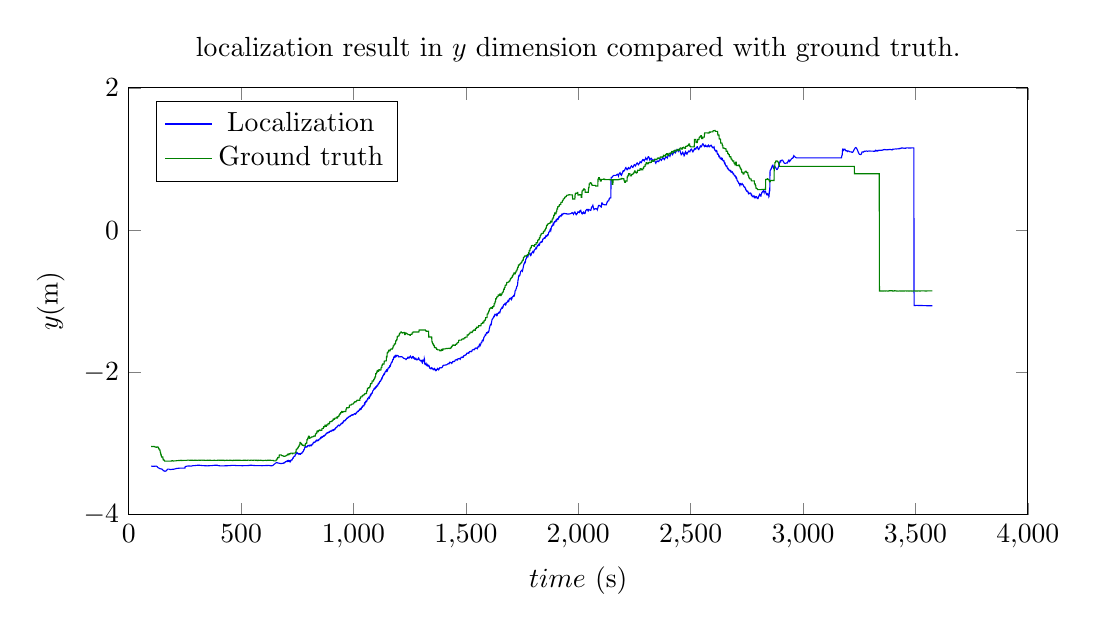
\begin{tikzpicture}

\begin{axis}[
title={localization result in $y$ dimension compared with ground truth.},
xlabel={$time$ (s)},
ylabel={$y$(m)},
xmin=0, xmax=4000,
ymin=-4, ymax=2,
axis on top,
width=13cm,
height=7cm,
legend style={at={(0.03,0.97)}, anchor=north west},
legend entries={{Localization},{Ground truth}}
]
\addplot [blue]
coordinates {
(100,-3.32057094573975)
(101,-3.31969237327576)
(102,-3.32051777839661)
(103,-3.32049226760864)
(104,-3.3204562664032)
(105,-3.32117342948914)
(106,-3.32172966003418)
(107,-3.32246994972229)
(108,-3.32260036468506)
(109,-3.32213425636292)
(110,-3.32183074951172)
(111,-3.32134008407593)
(112,-3.32117581367493)
(113,-3.32121562957764)
(114,-3.32129955291748)
(115,-3.3198356628418)
(116,-3.32022714614868)
(117,-3.32135677337647)
(118,-3.31991624832153)
(119,-3.32004022598267)
(120,-3.31885409355164)
(121,-3.31909656524658)
(122,-3.31930732727051)
(123,-3.32032585144043)
(124,-3.3209867477417)
(125,-3.32248544692993)
(126,-3.32592058181763)
(127,-3.32808136940002)
(128,-3.33337497711182)
(129,-3.33684158325195)
(130,-3.33943796157837)
(131,-3.34159731864929)
(132,-3.34409546852112)
(133,-3.34435224533081)
(134,-3.34651756286621)
(135,-3.3487720489502)
(136,-3.34966278076172)
(137,-3.35175681114197)
(138,-3.35375881195068)
(139,-3.35409903526306)
(140,-3.35606813430786)
(141,-3.35696291923523)
(142,-3.35859990119934)
(143,-3.35893559455872)
(144,-3.35852909088135)
(145,-3.35990977287293)
(146,-3.3598268032074)
(147,-3.36079621315002)
(148,-3.36176371574402)
(149,-3.36490058898926)
(150,-3.36580371856689)
(151,-3.37025737762451)
(152,-3.3747775554657)
(153,-3.37850403785706)
(154,-3.38194799423218)
(155,-3.38514304161072)
(156,-3.38432002067566)
(157,-3.38532829284668)
(158,-3.38569664955139)
(159,-3.38824534416199)
(160,-3.3902428150177)
(161,-3.39175367355347)
(162,-3.39207458496094)
(163,-3.3910653591156)
(164,-3.38984203338623)
(165,-3.38876056671143)
(166,-3.38671565055847)
(167,-3.38470482826233)
(168,-3.38194036483765)
(169,-3.37804436683655)
(170,-3.37519788742065)
(171,-3.37097573280335)
(172,-3.36749005317688)
(173,-3.3642783164978)
(174,-3.36274552345276)
(175,-3.36129307746887)
(176,-3.36079978942871)
(177,-3.3609037399292)
(178,-3.36144232749939)
(179,-3.36213898658752)
(180,-3.36290001869202)
(181,-3.36453294754028)
(182,-3.36527705192566)
(183,-3.366450548172)
(184,-3.36686944961548)
(185,-3.36745953559876)
(186,-3.36795687675476)
(187,-3.36782550811768)
(188,-3.36774682998657)
(189,-3.36609554290772)
(190,-3.36499738693237)
(191,-3.36497020721436)
(192,-3.36459517478943)
(193,-3.36418604850769)
(194,-3.36418867111206)
(195,-3.36411094665527)
(196,-3.36438727378845)
(197,-3.36449241638184)
(198,-3.36330151557922)
(199,-3.36348605155945)
(200,-3.3632504940033)
(201,-3.36239767074585)
(202,-3.36151051521301)
(203,-3.3608889579773)
(204,-3.35986232757568)
(205,-3.35909581184387)
(206,-3.35859942436218)
(207,-3.35821032524109)
(208,-3.35706806182861)
(209,-3.35678553581238)
(210,-3.35520505905151)
(211,-3.35385084152222)
(212,-3.35343718528748)
(213,-3.35300350189209)
(214,-3.35260248184204)
(215,-3.35223937034607)
(216,-3.35132169723511)
(217,-3.35064768791199)
(218,-3.35058975219727)
(219,-3.35020017623901)
(220,-3.34989356994629)
(221,-3.34941935539246)
(222,-3.34923315048218)
(223,-3.34875392913818)
(224,-3.34865164756775)
(225,-3.348788022995)
(226,-3.34839153289795)
(227,-3.348468542099)
(228,-3.3482096195221)
(229,-3.34819912910461)
(230,-3.34832692146301)
(231,-3.34809732437134)
(232,-3.34817147254944)
(233,-3.34813952445984)
(234,-3.34838008880615)
(235,-3.34800481796265)
(236,-3.34812736511231)
(237,-3.34772372245789)
(238,-3.34749555587769)
(239,-3.34745407104492)
(240,-3.34736514091492)
(241,-3.34736323356628)
(242,-3.34685659408569)
(243,-3.34740591049194)
(244,-3.34799647331238)
(245,-3.34798908233643)
(246,-3.34827017784119)
(247,-3.34819269180298)
(248,-3.34792566299439)
(249,-3.34752154350281)
(250,-3.34797191619873)
(251,-3.32800149917603)
(252,-3.32611870765686)
(253,-3.32563924789429)
(254,-3.32414484024048)
(255,-3.32285213470459)
(256,-3.32226228713989)
(257,-3.32138729095459)
(258,-3.32138729095459)
(259,-3.32032513618469)
(260,-3.31946969032288)
(261,-3.31915044784546)
(262,-3.31853890419006)
(263,-3.31784582138062)
(264,-3.31815004348755)
(265,-3.3180193901062)
(266,-3.31774139404297)
(267,-3.31743359565735)
(268,-3.31786274909973)
(269,-3.3182418346405)
(270,-3.31807732582092)
(271,-3.31732678413391)
(272,-3.31709432601929)
(273,-3.31784319877625)
(274,-3.31852579116821)
(275,-3.31927514076233)
(276,-3.31888890266419)
(277,-3.31941223144531)
(278,-3.31884670257568)
(279,-3.31822896003723)
(280,-3.31796956062317)
(281,-3.3164210319519)
(282,-3.31538987159729)
(283,-3.31501030921936)
(284,-3.31460762023926)
(285,-3.3141565322876)
(286,-3.3136990070343)
(287,-3.31307935714722)
(288,-3.31264424324036)
(289,-3.31254076957703)
(290,-3.31229591369629)
(291,-3.31203961372376)
(292,-3.31174826622009)
(293,-3.3117151260376)
(294,-3.31165766716003)
(295,-3.31167507171631)
(296,-3.31107831001282)
(297,-3.31102919578552)
(298,-3.31013178825378)
(299,-3.30954360961914)
(300,-3.30934381484985)
(301,-3.30896425247192)
(302,-3.30825233459473)
(303,-3.30801582336426)
(304,-3.30805397033691)
(305,-3.30773830413818)
(306,-3.30735921859741)
(307,-3.30734086036682)
(308,-3.30754137039185)
(309,-3.30697202682495)
(310,-3.30781888961792)
(311,-3.30774140357971)
(312,-3.30768442153931)
(313,-3.30793762207031)
(314,-3.30795621871948)
(315,-3.30687761306763)
(316,-3.30777192115784)
(317,-3.30796265602112)
(318,-3.30821228027344)
(319,-3.3087854385376)
(320,-3.30956935882568)
(321,-3.30996227264404)
(322,-3.31064820289612)
(323,-3.31105375289917)
(324,-3.31148934364319)
(325,-3.31133794784546)
(326,-3.31206941604614)
(327,-3.31183910369873)
(328,-3.31204509735107)
(329,-3.31247282028198)
(330,-3.31217479705811)
(331,-3.3127748966217)
(332,-3.31263184547424)
(333,-3.31250476837158)
(334,-3.31265735626221)
(335,-3.31258296966553)
(336,-3.31285119056702)
(337,-3.31335425376892)
(338,-3.31390881538391)
(339,-3.31383204460144)
(340,-3.31445813179016)
(341,-3.31407928466797)
(342,-3.31425547599793)
(343,-3.31452894210815)
(344,-3.3148934841156)
(345,-3.31455564498901)
(346,-3.31490015983582)
(347,-3.31584239006043)
(348,-3.31505703926086)
(349,-3.31512999534607)
(350,-3.31486630439758)
(351,-3.31564879417419)
(352,-3.31493353843689)
(353,-3.31500911712647)
(354,-3.31494450569153)
(355,-3.31407380104065)
(356,-3.31421399116516)
(357,-3.31440162658691)
(358,-3.31405639648438)
(359,-3.31330680847168)
(360,-3.31352257728577)
(361,-3.31319403648377)
(362,-3.31275486946106)
(363,-3.31264519691467)
(364,-3.31233906745911)
(365,-3.31231999397278)
(366,-3.31239771842957)
(367,-3.31187343597412)
(368,-3.31159806251526)
(369,-3.31190752983093)
(370,-3.31159973144531)
(371,-3.31154251098633)
(372,-3.31171894073486)
(373,-3.3107430934906)
(374,-3.31021547317505)
(375,-3.30955934524536)
(376,-3.30946898460388)
(377,-3.30937194824219)
(378,-3.30916261672974)
(379,-3.30850768089294)
(380,-3.30804657936096)
(381,-3.30816268920898)
(382,-3.30768465995789)
(383,-3.30783534049988)
(384,-3.3079981803894)
(385,-3.30784463882446)
(386,-3.30780911445618)
(387,-3.30773639678955)
(388,-3.30755519866943)
(389,-3.30726957321167)
(390,-3.30738186836243)
(391,-3.30568194389343)
(392,-3.30606555938721)
(393,-3.30642247200012)
(394,-3.30722689628601)
(395,-3.30779552459717)
(396,-3.30893158912659)
(397,-3.31049370765686)
(398,-3.31141948699951)
(399,-3.31218504905701)
(400,-3.31300091743469)
(401,-3.31311845779419)
(402,-3.31378269195557)
(403,-3.31442332267761)
(404,-3.31472206115723)
(405,-3.31450772285461)
(406,-3.31499886512756)
(407,-3.31500434875488)
(408,-3.31515383720398)
(409,-3.31555366516113)
(410,-3.31540465354919)
(411,-3.31549167633057)
(412,-3.31546998023987)
(413,-3.31562614440918)
(414,-3.3155562877655)
(415,-3.315838098526)
(416,-3.31600069999695)
(417,-3.31605434417725)
(418,-3.31664276123047)
(419,-3.31648898124695)
(420,-3.31641149520874)
(421,-3.31606912612915)
(422,-3.31626629829407)
(423,-3.31617379188538)
(424,-3.3159065246582)
(425,-3.3162579536438)
(426,-3.31570243835449)
(427,-3.31493639945984)
(428,-3.31478762626648)
(429,-3.31581354141235)
(430,-3.31627011299133)
(431,-3.31464576721191)
(432,-3.31423854827881)
(433,-3.3132905960083)
(434,-3.31365990638733)
(435,-3.31398797035217)
(436,-3.31347513198853)
(437,-3.31321859359741)
(438,-3.31315469741821)
(439,-3.31363463401794)
(440,-3.31314039230347)
(441,-3.31289386749268)
(442,-3.31290054321289)
(443,-3.3125741481781)
(444,-3.31272864341736)
(445,-3.31224012374878)
(446,-3.31212520599365)
(447,-3.31212949752808)
(448,-3.31234502792358)
(449,-3.3118908405304)
(450,-3.31179213523865)
(451,-3.31150317192078)
(452,-3.31140398979187)
(453,-3.31127572059631)
(454,-3.31075859069824)
(455,-3.31046581268311)
(456,-3.31054615974426)
(457,-3.30979299545288)
(458,-3.30934262275696)
(459,-3.3091926574707)
(460,-3.30961680412293)
(461,-3.30919361114502)
(462,-3.30904412269592)
(463,-3.30911183357239)
(464,-3.30896878242493)
(465,-3.30926156044006)
(466,-3.30895519256592)
(467,-3.30884075164795)
(468,-3.30882048606873)
(469,-3.30871367454529)
(470,-3.30849719047546)
(471,-3.30853414535523)
(472,-3.30929350852966)
(473,-3.309321641922)
(474,-3.30985522270203)
(475,-3.31038784980774)
(476,-3.31088066101074)
(477,-3.31119894981384)
(478,-3.31136178970337)
(479,-3.31161141395569)
(480,-3.31175184249878)
(481,-3.31197762489319)
(482,-3.31205534934998)
(483,-3.31216955184937)
(484,-3.31231474876404)
(485,-3.31241655349731)
(486,-3.31246113777161)
(487,-3.3125102519989)
(488,-3.31251645088196)
(489,-3.31257557868958)
(490,-3.3126277923584)
(491,-3.31264805793762)
(492,-3.31273746490479)
(493,-3.31291437149048)
(494,-3.3130567073822)
(495,-3.31275367736816)
(496,-3.31186985969544)
(497,-3.31165790557861)
(498,-3.31175208091736)
(499,-3.31175971031189)
(500,-3.3123733997345)
(501,-3.31247043609619)
(502,-3.31279277801514)
(503,-3.31411099433899)
(504,-3.31455421447754)
(505,-3.31416153907776)
(506,-3.31410336494446)
(507,-3.31458330154419)
(508,-3.31401038169861)
(509,-3.31288743019104)
(510,-3.31226205825806)
(511,-3.31297063827515)
(512,-3.31288146972656)
(513,-3.313063621521)
(514,-3.31325054168701)
(515,-3.31306004524231)
(516,-3.31306004524231)
(517,-3.31288981437683)
(518,-3.31292033195496)
(519,-3.31243538856506)
(520,-3.31271481513977)
(521,-3.3122820854187)
(522,-3.31223082542419)
(523,-3.31210374832153)
(524,-3.31189298629761)
(525,-3.31182169914246)
(526,-3.31182384490967)
(527,-3.31178665161133)
(528,-3.31166625022888)
(529,-3.31153774261475)
(530,-3.31100201606751)
(531,-3.31088542938232)
(532,-3.31069946289063)
(533,-3.31066393852234)
(534,-3.31046366691589)
(535,-3.31015682220459)
(536,-3.31018948554993)
(537,-3.30953192710877)
(538,-3.30910873413086)
(539,-3.3075954914093)
(540,-3.30648398399353)
(541,-3.30605697631836)
(542,-3.30643677711487)
(543,-3.3067057132721)
(544,-3.30709075927734)
(545,-3.30725932121277)
(546,-3.30710196495056)
(547,-3.30733489990234)
(548,-3.30746984481812)
(549,-3.30831074714661)
(550,-3.30821180343628)
(551,-3.30833292007446)
(552,-3.30874156951904)
(553,-3.30913043022156)
(554,-3.30968022346497)
(555,-3.30995917320252)
(556,-3.31044030189514)
(557,-3.31069421768189)
(558,-3.31092953681946)
(559,-3.31108927726746)
(560,-3.31140804290772)
(561,-3.31137800216675)
(562,-3.31143736839294)
(563,-3.31159782409668)
(564,-3.3117687702179)
(565,-3.31189560890198)
(566,-3.31208872795105)
(567,-3.31246519088745)
(568,-3.31217455863953)
(569,-3.31191825866699)
(570,-3.31201457977295)
(571,-3.31213521957398)
(572,-3.31252956390381)
(573,-3.31229710578919)
(574,-3.31218814849854)
(575,-3.31244778633118)
(576,-3.3124897480011)
(577,-3.31251311302185)
(578,-3.31274104118347)
(579,-3.31292200088501)
(580,-3.31295442581177)
(581,-3.31252884864807)
(582,-3.31233692169189)
(583,-3.31243848800659)
(584,-3.31214189529419)
(585,-3.31217551231384)
(586,-3.31288409233093)
(587,-3.31238698959351)
(588,-3.31250929832459)
(589,-3.31298422813416)
(590,-3.31320238113403)
(591,-3.31322693824768)
(592,-3.31354451179504)
(593,-3.31362223625183)
(594,-3.31348276138306)
(595,-3.31284594535828)
(596,-3.31279015541077)
(597,-3.31257724761963)
(598,-3.3124577999115)
(599,-3.31240558624268)
(600,-3.31213927268982)
(601,-3.31185841560364)
(602,-3.31210470199585)
(603,-3.31169509887695)
(604,-3.3117356300354)
(605,-3.31163859367371)
(606,-3.31163835525513)
(607,-3.31151127815247)
(608,-3.31160759925842)
(609,-3.31117963790894)
(610,-3.31111359596252)
(611,-3.31072282791138)
(612,-3.31091928482056)
(613,-3.31084704399109)
(614,-3.31058740615845)
(615,-3.310382604599)
(616,-3.31032180786133)
(617,-3.31056833267212)
(618,-3.31030178070068)
(619,-3.31031441688538)
(620,-3.31012105941773)
(621,-3.3103187084198)
(622,-3.30878067016602)
(623,-3.30979990959168)
(624,-3.30967497825623)
(625,-3.30911803245544)
(626,-3.31041979789734)
(627,-3.31146216392517)
(628,-3.31255578994751)
(629,-3.31299066543579)
(630,-3.31296753883362)
(631,-3.31421709060669)
(632,-3.31415438652039)
(633,-3.31456732749939)
(634,-3.31437516212463)
(635,-3.31515049934387)
(636,-3.31466579437256)
(637,-3.31391096115112)
(638,-3.31277060508728)
(639,-3.31217122077942)
(640,-3.31068634986877)
(641,-3.30964040756226)
(642,-3.30778861045837)
(643,-3.30506014823914)
(644,-3.30321359634399)
(645,-3.29960989952087)
(646,-3.29692053794861)
(647,-3.29354381561279)
(648,-3.2911639213562)
(649,-3.28880596160889)
(650,-3.28694939613342)
(651,-3.28299808502197)
(652,-3.28131675720215)
(653,-3.27898812294006)
(654,-3.27724456787109)
(655,-3.27535676956177)
(656,-3.27414894104004)
(657,-3.27233791351318)
(658,-3.27107715606689)
(659,-3.27106404304504)
(660,-3.2710428237915)
(661,-3.27100324630737)
(662,-3.27269434928894)
(663,-3.27362728118897)
(664,-3.27538537979126)
(665,-3.27604532241821)
(666,-3.27629542350769)
(667,-3.27639627456665)
(668,-3.27756142616272)
(669,-3.27872228622437)
(670,-3.2791223526001)
(671,-3.28027033805847)
(672,-3.28098130226135)
(673,-3.28192400932312)
(674,-3.28249144554138)
(675,-3.2822277545929)
(676,-3.2825186252594)
(677,-3.2825870513916)
(678,-3.28280735015869)
(679,-3.28276252746582)
(680,-3.28253483772278)
(681,-3.28251075744629)
(682,-3.28221487998962)
(683,-3.28163075447083)
(684,-3.28151702880859)
(685,-3.27984929084778)
(686,-3.27849984169006)
(687,-3.2773745059967)
(688,-3.27518749237061)
(689,-3.27779984474182)
(690,-3.27934503555298)
(691,-3.27510666847229)
(692,-3.26939678192139)
(693,-3.26777338981628)
(694,-3.2687304019928)
(695,-3.26907467842102)
(696,-3.2634265422821)
(697,-3.25961518287659)
(698,-3.25672030448914)
(699,-3.2556004524231)
(700,-3.25481104850769)
(701,-3.25608801841736)
(702,-3.25654053688049)
(703,-3.2538595199585)
(704,-3.24983477592468)
(705,-3.2440881729126)
(706,-3.24345469474793)
(707,-3.25071358680725)
(708,-3.24692511558533)
(709,-3.24166679382324)
(710,-3.24604201316834)
(711,-3.24195194244385)
(712,-3.2405641078949)
(713,-3.24308919906616)
(714,-3.25376749038696)
(715,-3.25642418861389)
(716,-3.25003671646118)
(717,-3.24485659599304)
(718,-3.24282503128052)
(719,-3.24624824523926)
(720,-3.25309610366821)
(721,-3.24568104743958)
(722,-3.23778796195984)
(723,-3.23253417015076)
(724,-3.23309063911438)
(725,-3.23511052131653)
(726,-3.235671043396)
(727,-3.22847557067871)
(728,-3.22036051750183)
(729,-3.21399664878845)
(730,-3.20733118057251)
(731,-3.2094030380249)
(732,-3.20687627792358)
(733,-3.19554424285889)
(734,-3.19177746772766)
(735,-3.1860523223877)
(736,-3.18051195144653)
(737,-3.18178105354309)
(738,-3.18277525901794)
(739,-3.18198561668396)
(740,-3.17507481575012)
(741,-3.16197562217712)
(742,-3.15440726280212)
(743,-3.14983177185059)
(744,-3.14726495742798)
(745,-3.14800906181335)
(746,-3.13988637924194)
(747,-3.13283276557922)
(748,-3.12637734413147)
(749,-3.12766075134277)
(750,-3.13225483894348)
(751,-3.13824534416199)
(752,-3.14354014396668)
(753,-3.14554786682129)
(754,-3.14303803443909)
(755,-3.14257502555847)
(756,-3.14548468589783)
(757,-3.15094804763794)
(758,-3.14634346961975)
(759,-3.14874458312988)
(760,-3.14694857597351)
(761,-3.14572525024414)
(762,-3.14838576316834)
(763,-3.15223526954651)
(764,-3.15243577957153)
(765,-3.14666032791138)
(766,-3.14172458648682)
(767,-3.13867735862732)
(768,-3.13772439956665)
(769,-3.13823747634888)
(770,-3.14028334617615)
(771,-3.13605165481567)
(772,-3.12646579742432)
(773,-3.12103867530823)
(774,-3.12153577804565)
(775,-3.1202986240387)
(776,-3.11397457122803)
(777,-3.10766053199768)
(778,-3.09827589988709)
(779,-3.089919090271)
(780,-3.09092044830322)
(781,-3.08429217338562)
(782,-3.07505226135254)
(783,-3.06219482421875)
(784,-3.05323529243469)
(785,-3.04693603515625)
(786,-3.0461049079895)
(787,-3.04760217666626)
(788,-3.05305290222168)
(789,-3.05441045761108)
(790,-3.05201625823975)
(791,-3.04865622520447)
(792,-3.04430031776428)
(793,-3.04593944549561)
(794,-3.0477340221405)
(795,-3.0409722328186)
(796,-3.03305959701538)
(797,-3.02891564369202)
(798,-3.02811098098755)
(799,-3.02801537513733)
(800,-3.03222703933716)
(801,-3.03520274162293)
(802,-3.03412818908691)
(803,-3.03225350379944)
(804,-3.02717995643616)
(805,-3.02550172805786)
(806,-3.03452062606812)
(807,-3.02875828742981)
(808,-3.02640223503113)
(809,-3.02567505836487)
(810,-3.02272748947144)
(811,-3.02226424217224)
(812,-3.02196455001831)
(813,-3.03147053718567)
(814,-3.02976179122925)
(815,-3.02262735366821)
(816,-3.01145482063294)
(817,-3.00790882110596)
(818,-3.0084855556488)
(819,-3.00955820083618)
(820,-3.00068330764771)
(821,-2.99247550964356)
(822,-2.98537087440491)
(823,-2.98173260688782)
(824,-2.98164963722229)
(825,-2.98320746421814)
(826,-2.98630523681641)
(827,-2.98729658126831)
(828,-2.98456978797913)
(829,-2.97714567184448)
(830,-2.97380685806274)
(831,-2.97479796409607)
(832,-2.9687647819519)
(833,-2.96326446533203)
(834,-2.95728230476379)
(835,-2.95374751091003)
(836,-2.95470952987671)
(837,-2.95738339424133)
(838,-2.96519255638123)
(839,-2.96423840522766)
(840,-2.96051025390625)
(841,-2.95421171188355)
(842,-2.95218420028687)
(843,-2.95177960395813)
(844,-2.95929455757141)
(845,-2.95765233039856)
(846,-2.94852542877197)
(847,-2.94142293930054)
(848,-2.93809819221497)
(849,-2.93688488006592)
(850,-2.94043135643005)
(851,-2.94015598297119)
(852,-2.9325704574585)
(853,-2.92347145080566)
(854,-2.91722679138184)
(855,-2.92084383964539)
(856,-2.92401027679443)
(857,-2.91601467132568)
(858,-2.91215038299561)
(859,-2.90730142593384)
(860,-2.9036295413971)
(861,-2.90389657020569)
(862,-2.90616703033447)
(863,-2.91092824935913)
(864,-2.90636157989502)
(865,-2.8991105556488)
(866,-2.8947913646698)
(867,-2.89232659339905)
(868,-2.89391160011292)
(869,-2.89826059341431)
(870,-2.89584851264954)
(871,-2.89188575744629)
(872,-2.8859281539917)
(873,-2.88293266296387)
(874,-2.88053941726685)
(875,-2.88270378112793)
(876,-2.88167190551758)
(877,-2.87451362609863)
(878,-2.86430907249451)
(879,-2.8599259853363)
(880,-2.862872838974)
(881,-2.86232018470764)
(882,-2.85744214057922)
(883,-2.85502886772156)
(884,-2.84711837768555)
(885,-2.84644436836243)
(886,-2.84733939170837)
(887,-2.85080051422119)
(888,-2.84992051124573)
(889,-2.84765267372131)
(890,-2.84212493896484)
(891,-2.83891701698303)
(892,-2.83558917045593)
(893,-2.83970594406128)
(894,-2.83550620079041)
(895,-2.83341121673584)
(896,-2.82873582839966)
(897,-2.82513570785523)
(898,-2.82727408409119)
(899,-2.83025741577148)
(900,-2.83191752433777)
(901,-2.82863616943359)
(902,-2.82719159126282)
(903,-2.82154369354248)
(904,-2.81752419471741)
(905,-2.82240915298462)
(906,-2.82072329521179)
(907,-2.81907248497009)
(908,-2.81239461898804)
(909,-2.80795812606812)
(910,-2.80795550346375)
(911,-2.8088436126709)
(912,-2.81565880775452)
(913,-2.81231904029846)
(914,-2.80965423583984)
(915,-2.80293774604797)
(916,-2.79745054244995)
(917,-2.79651808738709)
(918,-2.79944634437561)
(919,-2.79418301582336)
(920,-2.78886771202087)
(921,-2.781818151474)
(922,-2.77702689170837)
(923,-2.77497339248657)
(924,-2.77575349807739)
(925,-2.77632355690002)
(926,-2.77223634719849)
(927,-2.76438283920288)
(928,-2.75837016105652)
(929,-2.75881385803223)
(930,-2.75460076332092)
(931,-2.7499098777771)
(932,-2.74796652793884)
(933,-2.74502968788147)
(934,-2.74208331108093)
(935,-2.74335551261902)
(936,-2.74711871147156)
(937,-2.75207877159119)
(938,-2.74958205223084)
(939,-2.74689078330994)
(940,-2.74218678474426)
(941,-2.7393946647644)
(942,-2.73898482322693)
(943,-2.73580932617188)
(944,-2.72642850875855)
(945,-2.71964836120606)
(946,-2.71643805503845)
(947,-2.71634745597839)
(948,-2.71767091751099)
(949,-2.72150945663452)
(950,-2.71870875358582)
(951,-2.7151951789856)
(952,-2.70667386054993)
(953,-2.70203137397766)
(954,-2.70443725585938)
(955,-2.6955828666687)
(956,-2.688725233078)
(957,-2.68250417709351)
(958,-2.67856216430664)
(959,-2.67885422706604)
(960,-2.68437170982361)
(961,-2.68362069129944)
(962,-2.68233418464661)
(963,-2.67974519729614)
(964,-2.66920566558838)
(965,-2.6649227142334)
(966,-2.66388368606567)
(967,-2.6652843952179)
(968,-2.65888452529907)
(969,-2.65101218223572)
(970,-2.64571309089661)
(971,-2.64545321464539)
(972,-2.64647960662842)
(973,-2.64628171920776)
(974,-2.64403295516968)
(975,-2.63935303688049)
(976,-2.63054800033569)
(977,-2.63075089454651)
(978,-2.6322512626648)
(979,-2.62830138206482)
(980,-2.62584495544434)
(981,-2.62173509597778)
(982,-2.61752533912659)
(983,-2.61776041984558)
(984,-2.61855173110962)
(985,-2.62113928794861)
(986,-2.61769604682922)
(987,-2.61281490325928)
(988,-2.60639548301697)
(989,-2.60720252990723)
(990,-2.60782361030579)
(991,-2.60301351547241)
(992,-2.60128736495972)
(993,-2.59749174118042)
(994,-2.59609031677246)
(995,-2.59612059593201)
(996,-2.60207271575928)
(997,-2.60311508178711)
(998,-2.60136914253235)
(999,-2.59757614135742)
(1000,-2.59264492988586)
(1001,-2.59245371818543)
(1002,-2.59090614318848)
(1003,-2.58597111701965)
(1004,-2.58423328399658)
(1005,-2.58074831962585)
(1006,-2.58101963996887)
(1007,-2.58024454116821)
(1008,-2.58769965171814)
(1009,-2.58988881111145)
(1010,-2.58712530136108)
(1011,-2.57767534255981)
(1012,-2.57044434547424)
(1013,-2.56756091117859)
(1014,-2.57006072998047)
(1015,-2.5622878074646)
(1016,-2.55755519866943)
(1017,-2.54955124855042)
(1018,-2.54855442047119)
(1019,-2.54692435264587)
(1020,-2.55050563812256)
(1021,-2.55191040039063)
(1022,-2.54856109619141)
(1023,-2.54005575180054)
(1024,-2.53312253952026)
(1025,-2.53171634674072)
(1026,-2.53292584419251)
(1027,-2.52653121948242)
(1028,-2.52078914642334)
(1029,-2.51242780685425)
(1030,-2.51028823852539)
(1031,-2.50897073745728)
(1032,-2.51303124427795)
(1033,-2.52241349220276)
(1034,-2.51914072036743)
(1035,-2.50947499275208)
(1036,-2.49633860588074)
(1037,-2.48901867866516)
(1038,-2.4894905090332)
(1039,-2.49246549606323)
(1040,-2.48596620559692)
(1041,-2.47701859474182)
(1042,-2.47076749801636)
(1043,-2.46821284294128)
(1044,-2.46830439567566)
(1045,-2.47226977348328)
(1046,-2.47332644462585)
(1047,-2.46759486198425)
(1048,-2.45077252388001)
(1049,-2.43738770484924)
(1050,-2.44291043281555)
(1051,-2.44496417045593)
(1052,-2.43030142784119)
(1053,-2.42299151420593)
(1054,-2.40916156768799)
(1055,-2.40676999092102)
(1056,-2.40501165390015)
(1057,-2.40641450881958)
(1058,-2.41274571418762)
(1059,-2.40890336036682)
(1060,-2.39631080627441)
(1061,-2.38670015335083)
(1062,-2.37874627113342)
(1063,-2.38243246078491)
(1064,-2.38105130195618)
(1065,-2.36991572380066)
(1066,-2.36043906211853)
(1067,-2.35166788101196)
(1068,-2.34912991523743)
(1069,-2.3475615978241)
(1070,-2.35615634918213)
(1071,-2.36042213439941)
(1072,-2.34895491600037)
(1073,-2.3341052532196)
(1074,-2.32670879364014)
(1075,-2.31902480125427)
(1076,-2.32903218269348)
(1077,-2.32550597190857)
(1078,-2.31779026985169)
(1079,-2.30624628067017)
(1080,-2.2996096611023)
(1081,-2.29382133483887)
(1082,-2.29034638404846)
(1083,-2.29379487037659)
(1084,-2.28854727745056)
(1085,-2.27349948883057)
(1086,-2.26044487953186)
(1087,-2.25650072097778)
(1088,-2.25519418716431)
(1089,-2.25037884712219)
(1090,-2.24320292472839)
(1091,-2.23456144332886)
(1092,-2.22797870635986)
(1093,-2.22413349151611)
(1094,-2.22626280784607)
(1095,-2.23346948623657)
(1096,-2.23120141029358)
(1097,-2.22404456138611)
(1098,-2.2110116481781)
(1099,-2.20670628547669)
(1100,-2.20387077331543)
(1101,-2.21110343933106)
(1102,-2.20719408988953)
(1103,-2.20049643516541)
(1104,-2.18810677528381)
(1105,-2.18414878845215)
(1106,-2.18182015419006)
(1107,-2.17947387695313)
(1108,-2.18461513519287)
(1109,-2.17349767684937)
(1110,-2.16030263900757)
(1111,-2.15223073959351)
(1112,-2.15185070037842)
(1113,-2.16077423095703)
(1114,-2.15793776512146)
(1115,-2.14491724967957)
(1116,-2.13391399383545)
(1117,-2.12741565704346)
(1118,-2.1254985332489)
(1119,-2.12299394607544)
(1120,-2.12633872032166)
(1121,-2.1217885017395)
(1122,-2.11369633674622)
(1123,-2.10014891624451)
(1124,-2.09597849845886)
(1125,-2.08800959587097)
(1126,-2.09473490715027)
(1127,-2.09009718894959)
(1128,-2.07750844955444)
(1129,-2.06689095497131)
(1130,-2.05351829528809)
(1131,-2.0513653755188)
(1132,-2.04625535011292)
(1133,-2.0475378036499)
(1134,-2.04132509231567)
(1135,-2.02400135993958)
(1136,-2.01945352554321)
(1137,-2.02371597290039)
(1138,-2.02596020698547)
(1139,-2.01752948760986)
(1140,-2.00591611862183)
(1141,-1.99460077285767)
(1142,-1.98761558532715)
(1143,-1.98408210277557)
(1144,-1.98086285591126)
(1145,-1.98418581485748)
(1146,-1.98716688156128)
(1147,-1.97820830345154)
(1148,-1.96353149414063)
(1149,-1.9612489938736)
(1150,-1.9669486284256)
(1151,-1.97457718849182)
(1152,-1.96509265899658)
(1153,-1.95633339881897)
(1154,-1.94682478904724)
(1155,-1.93858695030212)
(1156,-1.93616223335266)
(1157,-1.93349289894104)
(1158,-1.9374589920044)
(1159,-1.93676006793976)
(1160,-1.92436397075653)
(1161,-1.91331470012665)
(1162,-1.90597867965698)
(1163,-1.90657591819763)
(1164,-1.91049158573151)
(1165,-1.90026950836182)
(1166,-1.88727247714996)
(1167,-1.87793922424316)
(1168,-1.86701261997223)
(1169,-1.86401700973511)
(1170,-1.85842931270599)
(1171,-1.86027026176453)
(1172,-1.85583257675171)
(1173,-1.84449779987335)
(1174,-1.8299252986908)
(1175,-1.8198539018631)
(1176,-1.82013130187988)
(1177,-1.81999433040619)
(1178,-1.80773186683655)
(1179,-1.79313027858734)
(1180,-1.7836012840271)
(1181,-1.77844488620758)
(1182,-1.78607153892517)
(1183,-1.78779602050781)
(1184,-1.79094529151917)
(1185,-1.78727519512177)
(1186,-1.77954375743866)
(1187,-1.76656413078308)
(1188,-1.76353228092194)
(1189,-1.77568745613098)
(1190,-1.77786684036255)
(1191,-1.77291941642761)
(1192,-1.7666482925415)
(1193,-1.76317644119263)
(1194,-1.76189517974854)
(1195,-1.76210522651672)
(1196,-1.76382851600647)
(1197,-1.76555037498474)
(1198,-1.76674139499664)
(1199,-1.76736342906952)
(1200,-1.78359746932983)
(1201,-1.78389537334442)
(1202,-1.78250873088837)
(1203,-1.78248643875122)
(1204,-1.78205752372742)
(1205,-1.78201067447662)
(1206,-1.78164577484131)
(1207,-1.78129374980927)
(1208,-1.7807834148407)
(1209,-1.78115093708038)
(1210,-1.78129613399506)
(1211,-1.78125834465027)
(1212,-1.78123033046722)
(1213,-1.78141272068024)
(1214,-1.78173589706421)
(1215,-1.78234004974365)
(1216,-1.7828004360199)
(1217,-1.78449428081513)
(1218,-1.78653085231781)
(1219,-1.78875124454498)
(1220,-1.79176998138428)
(1221,-1.79720675945282)
(1222,-1.79968559741974)
(1223,-1.80152821540833)
(1224,-1.80495655536652)
(1225,-1.80509340763092)
(1226,-1.80477452278137)
(1227,-1.80455899238586)
(1228,-1.80426263809204)
(1229,-1.80850410461426)
(1230,-1.81306385993958)
(1231,-1.81279361248016)
(1232,-1.81414318084717)
(1233,-1.81441295146942)
(1234,-1.81996595859528)
(1235,-1.81701159477234)
(1236,-1.80957186222076)
(1237,-1.80624771118164)
(1238,-1.80404281616211)
(1239,-1.80491173267365)
(1240,-1.80415678024292)
(1241,-1.79103517532349)
(1242,-1.79369604587555)
(1243,-1.79314005374909)
(1244,-1.79347252845764)
(1245,-1.78956246376038)
(1246,-1.79506742954254)
(1247,-1.80073809623718)
(1248,-1.79546320438385)
(1249,-1.7881578207016)
(1250,-1.78334391117096)
(1251,-1.78412914276123)
(1252,-1.78004121780396)
(1253,-1.77397656440735)
(1254,-1.7808347940445)
(1255,-1.78576803207398)
(1256,-1.78915250301361)
(1257,-1.79252648353577)
(1258,-1.79601180553436)
(1259,-1.80104470252991)
(1260,-1.79635715484619)
(1261,-1.78884339332581)
(1262,-1.78387939929962)
(1263,-1.78844857215881)
(1264,-1.78334760665894)
(1265,-1.77855026721954)
(1266,-1.78134882450104)
(1267,-1.79199886322022)
(1268,-1.79928541183472)
(1269,-1.79452443122864)
(1270,-1.7970449924469)
(1271,-1.81092619895935)
(1272,-1.81367409229279)
(1273,-1.80999290943146)
(1274,-1.80390536785126)
(1275,-1.80740416049957)
(1276,-1.81206858158112)
(1277,-1.80655145645142)
(1278,-1.80513441562653)
(1279,-1.81231355667114)
(1280,-1.82481646537781)
(1281,-1.8247241973877)
(1282,-1.82345843315125)
(1283,-1.82569658756256)
(1284,-1.82527422904968)
(1285,-1.81957983970642)
(1286,-1.81494808197022)
(1287,-1.81260216236115)
(1288,-1.81346297264099)
(1289,-1.80272698402405)
(1290,-1.7981538772583)
(1291,-1.80436384677887)
(1292,-1.81312739849091)
(1293,-1.82619571685791)
(1294,-1.82736587524414)
(1295,-1.82706725597382)
(1296,-1.8314323425293)
(1297,-1.83659374713898)
(1298,-1.83897793292999)
(1299,-1.83566951751709)
(1300,-1.8369265794754)
(1301,-1.83937561511993)
(1302,-1.83266973495483)
(1303,-1.83543431758881)
(1304,-1.84413313865662)
(1305,-1.85874509811401)
(1306,-1.86815083026886)
(1307,-1.87113082408905)
(1308,-1.85491514205933)
(1309,-1.82687020301819)
(1310,-1.82780730724335)
(1311,-1.83684229850769)
(1312,-1.84129250049591)
(1313,-1.84150469303131)
(1314,-1.84233510494232)
(1315,-1.80853939056397)
(1316,-1.82259833812714)
(1317,-1.87921917438507)
(1318,-1.88807928562164)
(1319,-1.8875515460968)
(1320,-1.89268445968628)
(1321,-1.89184772968292)
(1322,-1.87716019153595)
(1323,-1.87422478199005)
(1324,-1.8891566991806)
(1325,-1.89825642108917)
(1326,-1.90248537063599)
(1327,-1.89681601524353)
(1328,-1.8918799161911)
(1329,-1.9034595489502)
(1330,-1.91185283660889)
(1331,-1.91306877136231)
(1332,-1.91231286525726)
(1333,-1.91272282600403)
(1334,-1.90836560726166)
(1335,-1.90210008621216)
(1336,-1.90589475631714)
(1337,-1.91693508625031)
(1338,-1.93610632419586)
(1339,-1.93953907489777)
(1340,-1.93650388717651)
(1341,-1.93755340576172)
(1342,-1.94494724273682)
(1343,-1.94950759410858)
(1344,-1.9505649805069)
(1345,-1.9498598575592)
(1346,-1.94709813594818)
(1347,-1.94342863559723)
(1348,-1.93538892269135)
(1349,-1.93824875354767)
(1350,-1.94508898258209)
(1351,-1.95058012008667)
(1352,-1.95092952251434)
(1353,-1.94881308078766)
(1354,-1.9572319984436)
(1355,-1.96374547481537)
(1356,-1.96159064769745)
(1357,-1.95654797554016)
(1358,-1.9552149772644)
(1359,-1.95778095722199)
(1360,-1.9541107416153)
(1361,-1.94857621192932)
(1362,-1.955282330513)
(1363,-1.96471548080444)
(1364,-1.96867370605469)
(1365,-1.96581268310547)
(1366,-1.97076845169067)
(1367,-1.97790670394898)
(1368,-1.97616565227509)
(1369,-1.97118139266968)
(1370,-1.96169686317444)
(1371,-1.9589604139328)
(1372,-1.95961380004883)
(1373,-1.95585954189301)
(1374,-1.9454003572464)
(1375,-1.94772839546204)
(1376,-1.95526826381683)
(1377,-1.95846891403198)
(1378,-1.95882260799408)
(1379,-1.96446788311005)
(1380,-1.95970737934113)
(1381,-1.95417475700378)
(1382,-1.94638228416443)
(1383,-1.93820440769196)
(1384,-1.93564403057098)
(1385,-1.9392284154892)
(1386,-1.93743062019348)
(1387,-1.93745136260986)
(1388,-1.93634629249573)
(1389,-1.93614041805267)
(1390,-1.93625092506409)
(1391,-1.93675267696381)
(1392,-1.93628883361816)
(1393,-1.93504917621613)
(1394,-1.93300628662109)
(1395,-1.92651581764221)
(1396,-1.92534077167511)
(1397,-1.92121934890747)
(1398,-1.90523838996887)
(1399,-1.90308058261871)
(1400,-1.90165686607361)
(1401,-1.9008811712265)
(1402,-1.90086531639099)
(1403,-1.90062284469605)
(1404,-1.89951503276825)
(1405,-1.89918327331543)
(1406,-1.89911913871765)
(1407,-1.89818632602692)
(1408,-1.89802896976471)
(1409,-1.89772701263428)
(1410,-1.89820516109467)
(1411,-1.89723348617554)
(1412,-1.89681994915009)
(1413,-1.89580225944519)
(1414,-1.89456140995026)
(1415,-1.89353978633881)
(1416,-1.89133071899414)
(1417,-1.88901674747467)
(1418,-1.88618350028992)
(1419,-1.88218867778778)
(1420,-1.88171279430389)
(1421,-1.88087153434753)
(1422,-1.87604343891144)
(1423,-1.87423741817474)
(1424,-1.87460243701935)
(1425,-1.87969946861267)
(1426,-1.87531447410584)
(1427,-1.86668288707733)
(1428,-1.86243391036987)
(1429,-1.85784769058228)
(1430,-1.86089265346527)
(1431,-1.86245977878571)
(1432,-1.86241376399994)
(1433,-1.86621594429016)
(1434,-1.86758804321289)
(1435,-1.86655378341675)
(1436,-1.86891114711762)
(1437,-1.87518882751465)
(1438,-1.87239336967468)
(1439,-1.86416590213776)
(1440,-1.85628068447113)
(1441,-1.85042321681976)
(1442,-1.85275840759277)
(1443,-1.85195028781891)
(1444,-1.85101783275604)
(1445,-1.84848773479462)
(1446,-1.84717833995819)
(1447,-1.84427201747894)
(1448,-1.8460009098053)
(1449,-1.8477109670639)
(1450,-1.8472136259079)
(1451,-1.84153616428375)
(1452,-1.83522999286652)
(1453,-1.82614624500275)
(1454,-1.82463622093201)
(1455,-1.82532489299774)
(1456,-1.82437872886658)
(1457,-1.82228577136993)
(1458,-1.8256733417511)
(1459,-1.8251531124115)
(1460,-1.82382714748383)
(1461,-1.82048141956329)
(1462,-1.82842266559601)
(1463,-1.8281455039978)
(1464,-1.82099771499634)
(1465,-1.81220924854279)
(1466,-1.80823564529419)
(1467,-1.80720484256744)
(1468,-1.80754494667053)
(1469,-1.80807614326477)
(1470,-1.80692100524902)
(1471,-1.80907344818115)
(1472,-1.80860829353333)
(1473,-1.80657625198364)
(1474,-1.8102114200592)
(1475,-1.81520855426788)
(1476,-1.80827844142914)
(1477,-1.80363881587982)
(1478,-1.79520189762116)
(1479,-1.78876531124115)
(1480,-1.7888560295105)
(1481,-1.78923225402832)
(1482,-1.786860704422)
(1483,-1.78676092624664)
(1484,-1.78746294975281)
(1485,-1.78580260276795)
(1486,-1.7839572429657)
(1487,-1.79133105278015)
(1488,-1.78947424888611)
(1489,-1.78144347667694)
(1490,-1.77435398101807)
(1491,-1.76562666893005)
(1492,-1.7635669708252)
(1493,-1.76440238952637)
(1494,-1.76387345790863)
(1495,-1.76072144508362)
(1496,-1.76149487495422)
(1497,-1.7591290473938)
(1498,-1.75646197795868)
(1499,-1.75493907928467)
(1500,-1.757080078125)
(1501,-1.75462150573731)
(1502,-1.74792516231537)
(1503,-1.7375100851059)
(1504,-1.73180556297302)
(1505,-1.73219859600067)
(1506,-1.73261022567749)
(1507,-1.73008811473847)
(1508,-1.73027205467224)
(1509,-1.72907984256744)
(1510,-1.72671127319336)
(1511,-1.72521221637726)
(1512,-1.73088467121124)
(1513,-1.73259878158569)
(1514,-1.72462666034699)
(1515,-1.71729254722595)
(1516,-1.70849299430847)
(1517,-1.70785307884216)
(1518,-1.70808601379395)
(1519,-1.70668148994446)
(1520,-1.70786321163178)
(1521,-1.70953190326691)
(1522,-1.70784974098206)
(1523,-1.70507454872131)
(1524,-1.70674765110016)
(1525,-1.71003675460815)
(1526,-1.70687532424927)
(1527,-1.70001316070557)
(1528,-1.69195342063904)
(1529,-1.68461298942566)
(1530,-1.68417310714722)
(1531,-1.68474757671356)
(1532,-1.68205916881561)
(1533,-1.68022179603577)
(1534,-1.67924094200134)
(1535,-1.67796289920807)
(1536,-1.67712271213532)
(1537,-1.68017792701721)
(1538,-1.68277752399445)
(1539,-1.67967617511749)
(1540,-1.67143273353577)
(1541,-1.66560578346253)
(1542,-1.65986323356628)
(1543,-1.66128408908844)
(1544,-1.66237592697144)
(1545,-1.66034650802612)
(1546,-1.66034626960754)
(1547,-1.65983176231384)
(1548,-1.65741336345673)
(1549,-1.65928983688355)
(1550,-1.66531991958618)
(1551,-1.66786122322083)
(1552,-1.66184890270233)
(1553,-1.6507773399353)
(1554,-1.64213216304779)
(1555,-1.63701164722443)
(1556,-1.63730216026306)
(1557,-1.63776195049286)
(1558,-1.63989567756653)
(1559,-1.62100231647492)
(1560,-1.61482453346253)
(1561,-1.60444438457489)
(1562,-1.60614109039307)
(1563,-1.61485302448273)
(1564,-1.62237906455994)
(1565,-1.61582016944885)
(1566,-1.60581064224243)
(1567,-1.59078776836395)
(1568,-1.58471274375916)
(1569,-1.58459734916687)
(1570,-1.58180773258209)
(1571,-1.58186948299408)
(1572,-1.56187009811401)
(1573,-1.55112099647522)
(1574,-1.54695856571198)
(1575,-1.54768717288971)
(1576,-1.55323839187622)
(1577,-1.55536484718323)
(1578,-1.54285931587219)
(1579,-1.52785015106201)
(1580,-1.51023471355438)
(1581,-1.50618672370911)
(1582,-1.49823951721191)
(1583,-1.49785661697388)
(1584,-1.49303781986237)
(1585,-1.4856995344162)
(1586,-1.47665143013001)
(1587,-1.48009312152863)
(1588,-1.48049378395081)
(1589,-1.4737800359726)
(1590,-1.46365189552307)
(1591,-1.45027422904968)
(1592,-1.44307219982147)
(1593,-1.44468069076538)
(1594,-1.44421517848969)
(1595,-1.44893896579742)
(1596,-1.44456386566162)
(1597,-1.43788838386536)
(1598,-1.4324654340744)
(1599,-1.43040192127228)
(1600,-1.43842303752899)
(1601,-1.43599510192871)
(1602,-1.42367053031921)
(1603,-1.41035735607147)
(1604,-1.38878607749939)
(1605,-1.37682938575745)
(1606,-1.36601257324219)
(1607,-1.35042226314545)
(1608,-1.3429479598999)
(1609,-1.33045923709869)
(1610,-1.32588398456574)
(1611,-1.32847738265991)
(1612,-1.33205604553223)
(1613,-1.32510578632355)
(1614,-1.29754328727722)
(1615,-1.28196573257446)
(1616,-1.26608896255493)
(1617,-1.25523507595062)
(1618,-1.25130259990692)
(1619,-1.24981093406677)
(1620,-1.24373245239258)
(1621,-1.23836004734039)
(1622,-1.22884607315064)
(1623,-1.22624754905701)
(1624,-1.2161591053009)
(1625,-1.21945631504059)
(1626,-1.2189337015152)
(1627,-1.20966720581055)
(1628,-1.19376242160797)
(1629,-1.18716406822205)
(1630,-1.19061505794525)
(1631,-1.19317698478699)
(1632,-1.19198143482208)
(1633,-1.19060516357422)
(1634,-1.18725991249085)
(1635,-1.18247938156128)
(1636,-1.19496929645538)
(1637,-1.20193445682526)
(1638,-1.20575082302094)
(1639,-1.20276629924774)
(1640,-1.1932692527771)
(1641,-1.1807998418808)
(1642,-1.17263829708099)
(1643,-1.17142057418823)
(1644,-1.16805505752564)
(1645,-1.16927099227905)
(1646,-1.16318416595459)
(1647,-1.15778923034668)
(1648,-1.15213787555695)
(1649,-1.15131556987763)
(1650,-1.15666246414185)
(1651,-1.1613199710846)
(1652,-1.1537412405014)
(1653,-1.13940703868866)
(1654,-1.12444972991943)
(1655,-1.11245822906494)
(1656,-1.11123275756836)
(1657,-1.109206199646)
(1658,-1.10690891742706)
(1659,-1.10064136981964)
(1660,-1.0941721200943)
(1661,-1.08303070068359)
(1662,-1.08212220668793)
(1663,-1.08393490314484)
(1664,-1.09166836738586)
(1665,-1.08637821674347)
(1666,-1.07088088989258)
(1667,-1.05973017215729)
(1668,-1.05079460144043)
(1669,-1.05024909973145)
(1670,-1.04947459697723)
(1671,-1.04493319988251)
(1672,-1.04406547546387)
(1673,-1.03761756420136)
(1674,-1.03289353847504)
(1675,-1.04249703884125)
(1676,-1.05090439319611)
(1677,-1.05421161651611)
(1678,-1.04804837703705)
(1679,-1.03730010986328)
(1680,-1.02254128456116)
(1681,-1.01924288272858)
(1682,-1.01729035377503)
(1683,-1.0161167383194)
(1684,-1.01440012454987)
(1685,-1.01006257534027)
(1686,-0.999265491962434)
(1687,-0.993789792060853)
(1688,-1.00073909759522)
(1689,-1.00449633598328)
(1690,-1.00610542297363)
(1691,-0.999558806419373)
(1692,-0.98397308588028)
(1693,-0.973309695720673)
(1694,-0.964515388011933)
(1695,-0.966869950294495)
(1696,-0.970118820667268)
(1697,-0.968823015689851)
(1698,-0.963649034500123)
(1699,-0.960571110248566)
(1700,-0.956263184547425)
(1701,-0.954174160957337)
(1702,-0.966903626918794)
(1703,-0.976141393184663)
(1704,-0.96972155570984)
(1705,-0.961745440959931)
(1706,-0.945256412029267)
(1707,-0.93923842906952)
(1708,-0.936554968357087)
(1709,-0.934919595718385)
(1710,-0.935785472393037)
(1711,-0.935078203678132)
(1712,-0.924418568611146)
(1713,-0.918294489383698)
(1714,-0.921002388000489)
(1715,-0.925679445266724)
(1716,-0.920089960098267)
(1717,-0.904870748519898)
(1718,-0.885214984416962)
(1719,-0.858098447322846)
(1720,-0.84900575876236)
(1721,-0.846088230609895)
(1722,-0.845308840274812)
(1723,-0.830549716949464)
(1724,-0.825163424015046)
(1725,-0.818482756614686)
(1726,-0.795717716217042)
(1727,-0.793296396732331)
(1728,-0.788106203079224)
(1729,-0.781341195106507)
(1730,-0.767290353775025)
(1731,-0.733473896980286)
(1732,-0.703059136867524)
(1733,-0.694392502307893)
(1734,-0.666799664497376)
(1735,-0.645703494548798)
(1736,-0.640753030776978)
(1737,-0.635071754455567)
(1738,-0.636900365352631)
(1739,-0.642005503177644)
(1740,-0.63944298028946)
(1741,-0.623614788055421)
(1742,-0.605802893638612)
(1743,-0.589970231056214)
(1744,-0.5813307762146)
(1745,-0.57777363061905)
(1746,-0.576769351959229)
(1747,-0.571241140365601)
(1748,-0.571342885494233)
(1749,-0.565712749958039)
(1750,-0.559411585330964)
(1751,-0.55874389410019)
(1752,-0.570624589920045)
(1753,-0.560284197330476)
(1754,-0.54002606868744)
(1755,-0.527141749858857)
(1756,-0.51105809211731)
(1757,-0.495745539665223)
(1758,-0.482027649879456)
(1759,-0.477913469076157)
(1760,-0.46590805053711)
(1761,-0.458212912082673)
(1762,-0.465403884649278)
(1763,-0.461144953966142)
(1764,-0.454817116260529)
(1765,-0.445431381464005)
(1766,-0.41896489262581)
(1767,-0.405502289533616)
(1768,-0.403102904558183)
(1769,-0.399326980113984)
(1770,-0.394536405801774)
(1771,-0.373588979244233)
(1772,-0.367478907108308)
(1773,-0.364751875400544)
(1774,-0.363879919052125)
(1775,-0.367672920227052)
(1776,-0.37320226430893)
(1777,-0.363175570964814)
(1778,-0.348758935928346)
(1779,-0.340175986289979)
(1780,-0.336697280406953)
(1781,-0.336750566959382)
(1782,-0.334409952163697)
(1783,-0.332947701215745)
(1784,-0.334364354610444)
(1785,-0.331760525703431)
(1786,-0.344838678836823)
(1787,-0.354033380746842)
(1788,-0.360143989324571)
(1789,-0.358222097158433)
(1790,-0.35120776295662)
(1791,-0.341919213533402)
(1792,-0.327801287174226)
(1793,-0.320975482463838)
(1794,-0.321233808994294)
(1795,-0.318077951669694)
(1796,-0.314394623041154)
(1797,-0.306225866079331)
(1798,-0.300895959138871)
(1799,-0.305427819490434)
(1800,-0.305806189775468)
(1801,-0.314675480127335)
(1802,-0.308749049901963)
(1803,-0.298813790082932)
(1804,-0.287119120359422)
(1805,-0.277570128440858)
(1806,-0.275267690420152)
(1807,-0.274396836757661)
(1808,-0.271273404359818)
(1809,-0.26442649960518)
(1810,-0.259905695915223)
(1811,-0.252602428197862)
(1812,-0.259241104125977)
(1813,-0.263368278741837)
(1814,-0.262893527746201)
(1815,-0.251755684614182)
(1816,-0.238803058862687)
(1817,-0.224067836999894)
(1818,-0.219921737909318)
(1819,-0.223242402076722)
(1820,-0.220909491181374)
(1821,-0.218444034457208)
(1822,-0.213119253516198)
(1823,-0.20730845630169)
(1824,-0.202802389860154)
(1825,-0.208307921886445)
(1826,-0.215751007199288)
(1827,-0.21326780319214)
(1828,-0.205529779195786)
(1829,-0.186579063534737)
(1830,-0.176990017294885)
(1831,-0.173091620206834)
(1832,-0.174444183707238)
(1833,-0.172289222478867)
(1834,-0.170041114091874)
(1835,-0.165487438440324)
(1836,-0.160952702164651)
(1837,-0.164780974388123)
(1838,-0.169512927532197)
(1839,-0.168135002255441)
(1840,-0.161943942308427)
(1841,-0.149977028369904)
(1842,-0.131242230534554)
(1843,-0.125034734606744)
(1844,-0.124438241124154)
(1845,-0.12230046838522)
(1846,-0.121276140213014)
(1847,-0.116139948368073)
(1848,-0.113117434084416)
(1849,-0.109060406684876)
(1850,-0.105918519198895)
(1851,-0.108318760991097)
(1852,-0.113344028592111)
(1853,-0.112162470817567)
(1854,-0.0989460349082956)
(1855,-0.0903575494885453)
(1856,-0.08073315024376)
(1857,-0.0826352164149293)
(1858,-0.0882869511842736)
(1859,-0.0897574499249467)
(1860,-0.0841582417488107)
(1861,-0.078410580754281)
(1862,-0.0702204629778871)
(1863,-0.065575748682023)
(1864,-0.0650680065155038)
(1865,-0.0711407884955415)
(1866,-0.0678432062268266)
(1867,-0.0547988899052152)
(1868,-0.0384176895022401)
(1869,-0.0282641910016546)
(1870,-0.0249618925154218)
(1871,-0.0236825272440919)
(1872,-0.0244595371186742)
(1873,-0.0172236636281022)
(1874,-0.00502720475196927)
(1875,0.00901734456419856)
(1876,0.013127986341714)
(1877,0.0037364261224857)
(1878,-0.00416298024356454)
(1879,0.0142118968069544)
(1880,0.0313725322484961)
(1881,0.0455604605376711)
(1882,0.0544164702296248)
(1883,0.0569564141333094)
(1884,0.0602958314120761)
(1885,0.0587242990732184)
(1886,0.0641920045018187)
(1887,0.0762597471475592)
(1888,0.0869013667106619)
(1889,0.0912262722849837)
(1890,0.0878029912710181)
(1891,0.0804439932107916)
(1892,0.0942273736000052)
(1893,0.104392766952514)
(1894,0.116940699517726)
(1895,0.12221698462963)
(1896,0.12229574471712)
(1897,0.122085027396678)
(1898,0.116294056177138)
(1899,0.1167224496603)
(1900,0.13060563802719)
(1901,0.141770988702773)
(1902,0.144628033041953)
(1903,0.135424673557281)
(1904,0.131363287568091)
(1905,0.144270360469817)
(1906,0.151871174573897)
(1907,0.161390125751494)
(1908,0.163581103086471)
(1909,0.16279301047325)
(1910,0.163198024034499)
(1911,0.155455097556113)
(1912,0.160566598176955)
(1913,0.180227369070052)
(1914,0.187563106417655)
(1915,0.188002496957778)
(1916,0.182855963706969)
(1917,0.182252123951911)
(1918,0.193107873201369)
(1919,0.200931936502456)
(1920,0.202410757541656)
(1921,0.204719156026839)
(1922,0.205996125936507)
(1923,0.204974427819251)
(1924,0.199627816677093)
(1925,0.206605449318885)
(1926,0.21818247437477)
(1927,0.22568443417549)
(1928,0.226333335041999)
(1929,0.220472276210784)
(1930,0.215263560414313)
(1931,0.219267353415488)
(1932,0.225888431072234)
(1933,0.229287862777709)
(1934,0.231102660298347)
(1935,0.233097046613692)
(1936,0.233596637845038)
(1937,0.233000695705413)
(1938,0.233384028077125)
(1939,0.234027221798896)
(1940,0.234678775072097)
(1941,0.232624724507331)
(1942,0.230936914682387)
(1943,0.230905935168265)
(1944,0.230760365724563)
(1945,0.230101987719535)
(1946,0.230050891637801)
(1947,0.229494810104369)
(1948,0.229649752378463)
(1949,0.228961929678916)
(1950,0.225335344672202)
(1951,0.225496903061866)
(1952,0.225531429052352)
(1953,0.225501850247382)
(1954,0.225584506988524)
(1955,0.225804224610328)
(1956,0.226057291030883)
(1957,0.226241409778594)
(1958,0.226371899247169)
(1959,0.226563647389411)
(1960,0.227184683084487)
(1961,0.227917611598968)
(1962,0.228341281414031)
(1963,0.229272171854972)
(1964,0.229962930083274)
(1965,0.230478182435035)
(1966,0.230900362133979)
(1967,0.231853038072585)
(1968,0.2329194098711)
(1969,0.234810456633567)
(1970,0.237231850624084)
(1971,0.242052257061004)
(1972,0.245521947741508)
(1973,0.246393337845801)
(1974,0.243231087923049)
(1975,0.236946016550063)
(1976,0.233527272939681)
(1977,0.235071659088134)
(1978,0.232845753431319)
(1979,0.225608691573142)
(1980,0.234098806977271)
(1981,0.242204323410987)
(1982,0.246396854519843)
(1983,0.245072677731513)
(1984,0.249401226639747)
(1985,0.254105955362319)
(1986,0.246642753481864)
(1987,0.242672577500342)
(1988,0.231877461075782)
(1989,0.226234152913093)
(1990,0.22148385643959)
(1991,0.214382857084273)
(1992,0.215040877461432)
(1993,0.222065433859824)
(1994,0.232706770300864)
(1995,0.236456036567687)
(1996,0.23569719493389)
(1997,0.24447813630104)
(1998,0.255644381046294)
(1999,0.256819784641265)
(2000,0.254070818424224)
(2001,0.251820236444472)
(2002,0.255434095859527)
(2003,0.25630286335945)
(2004,0.248599216341971)
(2005,0.24728974699974)
(2006,0.25915092229843)
(2007,0.270812481641768)
(2008,0.273160904645919)
(2009,0.270007640123366)
(2010,0.274205684661864)
(2011,0.277504742145537)
(2012,0.263473689556121)
(2013,0.253151714801787)
(2014,0.24802117049694)
(2015,0.239410519599914)
(2016,0.23419153690338)
(2017,0.228553488850593)
(2018,0.227777272462844)
(2019,0.237655237317084)
(2020,0.243475496768951)
(2021,0.243227750062942)
(2022,0.240980744361877)
(2023,0.250490814447402)
(2024,0.253597974777221)
(2025,0.248366713523864)
(2026,0.243128985166549)
(2027,0.235704824328422)
(2028,0.232501298189162)
(2029,0.232957407832145)
(2030,0.232430219650268)
(2031,0.243255332112311)
(2032,0.258131772279738)
(2033,0.270409137010573)
(2034,0.27635359764099)
(2035,0.278103262186049)
(2036,0.283440321683883)
(2037,0.288815110921859)
(2038,0.289956390857696)
(2039,0.284664958715438)
(2040,0.284719347953795)
(2041,0.288373053073882)
(2042,0.28475460410118)
(2043,0.272682398557662)
(2044,0.269090145826339)
(2045,0.284510344266891)
(2046,0.289692699909209)
(2047,0.291379392147063)
(2048,0.286078572273253)
(2049,0.283573329448699)
(2050,0.283244431018828)
(2051,0.281251460313796)
(2052,0.282814055681228)
(2053,0.281510055065154)
(2054,0.28016036748886)
(2055,0.276638388633727)
(2056,0.277997404336928)
(2057,0.289779484272002)
(2058,0.304206162691115)
(2059,0.321012705564498)
(2060,0.324419438838958)
(2061,0.324590027332305)
(2062,0.327934324741363)
(2063,0.327728152275085)
(2064,0.341871798038482)
(2065,0.348774552345275)
(2066,0.336851716041564)
(2067,0.321246713399886)
(2068,0.305247038602828)
(2069,0.30292585492134)
(2070,0.289178490638732)
(2071,0.293031662702559)
(2072,0.295518189668654)
(2073,0.297312080860137)
(2074,0.297438144683837)
(2075,0.298275023698806)
(2076,0.299622535705565)
(2077,0.300067156553267)
(2078,0.299987316131591)
(2079,0.298431754112243)
(2080,0.296092778444289)
(2081,0.29696089029312)
(2082,0.298188269138335)
(2083,0.300197094678878)
(2084,0.302107751369475)
(2085,0.289301306009292)
(2086,0.298850029706954)
(2087,0.307066917419433)
(2088,0.317518383264541)
(2089,0.334087252616881)
(2090,0.342481583356856)
(2091,0.346440792083739)
(2092,0.348523527383803)
(2093,0.348390609025954)
(2094,0.347148865461349)
(2095,0.344874799251555)
(2096,0.341148763895034)
(2097,0.337885320186614)
(2098,0.335431277751922)
(2099,0.333186477422713)
(2100,0.329298019409179)
(2101,0.32725504040718)
(2102,0.325013279914855)
(2103,0.323518693447112)
(2104,0.380006670951842)
(2105,0.379700690507888)
(2106,0.380155682563781)
(2107,0.380182355642318)
(2108,0.371947705745696)
(2109,0.367364585399627)
(2110,0.363236993551253)
(2111,0.360160768032073)
(2112,0.358550488948821)
(2113,0.35809826850891)
(2114,0.357925176620482)
(2115,0.357222199440001)
(2116,0.356609344482421)
(2117,0.356067031621932)
(2118,0.355734199285506)
(2119,0.3559972345829)
(2120,0.355615884065627)
(2121,0.355432957410811)
(2122,0.354961812496184)
(2123,0.35496038198471)
(2124,0.354937702417373)
(2125,0.355256170034408)
(2126,0.370094716548919)
(2127,0.382914662361144)
(2128,0.383045583963393)
(2129,0.395038902759551)
(2130,0.406554758548736)
(2131,0.407312065362929)
(2132,0.408039063215255)
(2133,0.409021407365798)
(2134,0.410340636968612)
(2135,0.411305189132689)
(2136,0.412402600049972)
(2137,0.438978791236876)
(2138,0.440013378858565)
(2139,0.440706998109817)
(2140,0.450457274913787)
(2141,0.451075255870818)
(2142,0.451913505792617)
(2143,0.452709466218947)
(2144,0.453024685382842)
(2145,0.453592956066131)
(2146,0.739278614521026)
(2147,0.739253222942351)
(2148,0.739488184452056)
(2149,0.740343987941741)
(2150,0.740684568881988)
(2151,0.745882034301757)
(2152,0.750330746173858)
(2153,0.75337666273117)
(2154,0.756314456462859)
(2155,0.764066159725188)
(2156,0.765225887298583)
(2157,0.76757264137268)
(2158,0.768028259277343)
(2159,0.768961012363433)
(2160,0.769742488861083)
(2161,0.769988179206847)
(2162,0.769065141677855)
(2163,0.768869280815124)
(2164,0.769094467163085)
(2165,0.769557714462279)
(2166,0.769781410694121)
(2167,0.769671440124511)
(2168,0.770798206329345)
(2169,0.772446811199187)
(2170,0.775000751018523)
(2171,0.777291178703307)
(2172,0.78119933605194)
(2173,0.784196376800536)
(2174,0.785122513771056)
(2175,0.777662932872771)
(2176,0.77593183517456)
(2177,0.77858155965805)
(2178,0.774066150188445)
(2179,0.761933207511901)
(2180,0.773251235485076)
(2181,0.786445260047912)
(2182,0.793236732482909)
(2183,0.796784281730651)
(2184,0.796658158302306)
(2185,0.804684996604918)
(2186,0.80756253004074)
(2187,0.800421953201293)
(2188,0.792069673538207)
(2189,0.780346810817718)
(2190,0.777834177017211)
(2191,0.775240123271941)
(2192,0.76989185810089)
(2193,0.773860156536101)
(2194,0.783066809177398)
(2195,0.797887325286864)
(2196,0.802014112472533)
(2197,0.804775476455687)
(2198,0.817367613315581)
(2199,0.83145236968994)
(2200,0.833321571350097)
(2201,0.829765498638152)
(2202,0.828343868255614)
(2203,0.834591984748839)
(2204,0.834912717342376)
(2205,0.833931028842925)
(2206,0.840326011180877)
(2207,0.849852085113524)
(2208,0.857008457183837)
(2209,0.861658990383147)
(2210,0.865316987037658)
(2211,0.876131653785705)
(2212,0.879287719726562)
(2213,0.871943950653075)
(2214,0.863457977771758)
(2215,0.85990536212921)
(2216,0.858286201953887)
(2217,0.847736477851867)
(2218,0.84825712442398)
(2219,0.854237854480742)
(2220,0.863456726074218)
(2221,0.867817997932433)
(2222,0.865693926811217)
(2223,0.875215888023375)
(2224,0.870394527912139)
(2225,0.874441981315612)
(2226,0.871868848800658)
(2227,0.867684602737426)
(2228,0.870932817459105)
(2229,0.871453940868377)
(2230,0.865801870822905)
(2231,0.869929075241088)
(2232,0.878365337848662)
(2233,0.885620892047881)
(2234,0.889257073402404)
(2235,0.892386436462401)
(2236,0.900238573551177)
(2237,0.903428137302398)
(2238,0.898745238780974)
(2239,0.894184231758117)
(2240,0.889824211597442)
(2241,0.888562381267547)
(2242,0.881279408931731)
(2243,0.880026996135711)
(2244,0.887725591659545)
(2245,0.89622664451599)
(2246,0.901389241218566)
(2247,0.900522530078887)
(2248,0.908356845378875)
(2249,0.920480966567992)
(2250,0.921264171600341)
(2251,0.916691958904265)
(2252,0.912693977355956)
(2253,0.911611974239348)
(2254,0.909494459629058)
(2255,0.903467714786529)
(2256,0.909811973571776)
(2257,0.918549954891204)
(2258,0.926435291767119)
(2259,0.93041831254959)
(2260,0.935207784175872)
(2261,0.942400038242339)
(2262,0.944863617420196)
(2263,0.940945088863372)
(2264,0.933085143566131)
(2265,0.93151694536209)
(2266,0.924157798290252)
(2267,0.919963240623473)
(2268,0.917760670185088)
(2269,0.922944247722625)
(2270,0.931583940982818)
(2271,0.936934649944304)
(2272,0.937184333801269)
(2273,0.944010913372039)
(2274,0.95374822616577)
(2275,0.962663888931273)
(2276,0.960430145263671)
(2277,0.953380048274993)
(2278,0.950844109058379)
(2279,0.948658406734466)
(2280,0.9469096660614)
(2281,0.949008524417876)
(2282,0.957641303539275)
(2283,0.966737091541289)
(2284,0.976379573345183)
(2285,0.977403998374938)
(2286,0.984583973884582)
(2287,0.991871237754821)
(2288,0.993175327777862)
(2289,0.990424692630767)
(2290,0.983845889568328)
(2291,0.986909627914428)
(2292,0.984881877899169)
(2293,0.978299558162688)
(2294,0.974665820598601)
(2295,0.981431603431701)
(2296,0.989513158798217)
(2297,0.992614626884459)
(2298,0.995283603668212)
(2299,1.00579071044922)
(2300,1.01391506195068)
(2301,1.00503396987915)
(2302,1.00051712989807)
(2303,0.997984111309051)
(2304,1.00182008743286)
(2305,0.999936521053313)
(2306,0.991097748279571)
(2307,1.00077593326568)
(2308,1.0073561668396)
(2309,1.01413476467132)
(2310,1.02330207824707)
(2311,1.02854084968567)
(2312,1.03291022777557)
(2313,1.03269445896149)
(2314,1.02908682823181)
(2315,1.01731181144714)
(2316,1.00920557975769)
(2317,0.997235357761382)
(2318,0.984188854694365)
(2319,0.985288619995116)
(2320,0.994680583477019)
(2321,0.999863564968108)
(2322,1.00310015678406)
(2323,1.00447201728821)
(2324,1.010373711586)
(2325,1.01071763038635)
(2326,1.00063991546631)
(2327,0.999302327632903)
(2328,0.988307833671569)
(2329,0.990394115447997)
(2330,0.983381509780883)
(2331,0.973348438739776)
(2332,0.975812256336211)
(2333,0.985294938087462)
(2334,0.985721826553344)
(2335,0.984068512916564)
(2336,0.9851216673851)
(2337,0.988571166992187)
(2338,0.985939443111419)
(2339,0.980229198932647)
(2340,0.977366149425506)
(2341,0.968571424484252)
(2342,0.964285373687743)
(2343,0.954835772514342)
(2344,0.944037437438964)
(2345,0.939388811588286)
(2346,0.950277566909789)
(2347,0.956126451492309)
(2348,0.95843470096588)
(2349,0.962799429893493)
(2350,0.968836903572082)
(2351,0.971344351768493)
(2352,0.972467422485351)
(2353,0.970587253570556)
(2354,0.965766489505767)
(2355,0.966790854930877)
(2356,0.967938303947448)
(2357,0.963829040527343)
(2358,0.962971806526183)
(2359,0.970695614814757)
(2360,0.978339195251464)
(2361,0.982516229152678)
(2362,0.986039400100707)
(2363,0.991071343421935)
(2364,0.996524274349212)
(2365,0.997180521488189)
(2366,0.994653463363646)
(2367,0.9900603890419)
(2368,0.991668283939361)
(2369,0.987715661525725)
(2370,0.98181003332138)
(2371,0.986403465270995)
(2372,0.993255376815795)
(2373,1.00188231468201)
(2374,1.00259029865265)
(2375,1.00787544250488)
(2376,1.01435089111328)
(2377,1.01666617393494)
(2378,1.01308143138885)
(2379,1.00745368003845)
(2380,1.00310087203979)
(2381,1.00449550151825)
(2382,0.99896878004074)
(2383,0.991640210151671)
(2384,0.99554282426834)
(2385,1.00343799591064)
(2386,1.00924456119537)
(2387,1.0147967338562)
(2388,1.0190167427063)
(2389,1.02629363536835)
(2390,1.02932214736938)
(2391,1.02880871295929)
(2392,1.02377450466156)
(2393,1.02346658706665)
(2394,1.02538621425629)
(2395,1.01955652236938)
(2396,1.01361846923828)
(2397,1.02131974697113)
(2398,1.03109514713287)
(2399,1.03821527957916)
(2400,1.04189467430115)
(2401,1.05090463161468)
(2402,1.05798768997192)
(2403,1.05594432353973)
(2404,1.05140960216522)
(2405,1.04893445968628)
(2406,1.05208444595337)
(2407,1.04352414608002)
(2408,1.03804790973663)
(2409,1.04797530174255)
(2410,1.05509853363037)
(2411,1.06410992145538)
(2412,1.07143986225128)
(2413,1.0796263217926)
(2414,1.08499705791473)
(2415,1.08172905445099)
(2416,1.07801711559296)
(2417,1.07536160945892)
(2418,1.07789516448974)
(2419,1.0700443983078)
(2420,1.06251323223114)
(2421,1.07038795948028)
(2422,1.07734954357147)
(2423,1.08355844020843)
(2424,1.09034073352814)
(2425,1.09453415870666)
(2426,1.10365116596222)
(2427,1.10257029533386)
(2428,1.09904932975769)
(2429,1.09555613994598)
(2430,1.09783804416656)
(2431,1.09383988380432)
(2432,1.08637261390686)
(2433,1.09052419662475)
(2434,1.09995698928833)
(2435,1.1063529253006)
(2436,1.1122727394104)
(2437,1.11731398105621)
(2438,1.12608456611633)
(2439,1.1308661699295)
(2440,1.12597131729126)
(2441,1.12230741977692)
(2442,1.12082767486572)
(2443,1.12475216388702)
(2444,1.11373674869537)
(2445,1.10619819164276)
(2446,1.11166989803314)
(2447,1.11984384059906)
(2448,1.12610423564911)
(2449,1.12977159023285)
(2450,1.13170874118805)
(2451,1.13655531406402)
(2452,1.12626981735229)
(2453,1.12067222595215)
(2454,1.09495282173157)
(2455,1.09252989292145)
(2456,1.07899451255798)
(2457,1.07351768016815)
(2458,1.05911576747894)
(2459,1.0591276884079)
(2460,1.06682693958282)
(2461,1.07528746128082)
(2462,1.07713735103607)
(2463,1.08022105693817)
(2464,1.09017443656921)
(2465,1.09547781944275)
(2466,1.09063518047333)
(2467,1.074174284935)
(2468,1.06690192222595)
(2469,1.06532382965088)
(2470,1.05666697025299)
(2471,1.04411911964416)
(2472,1.04804372787475)
(2473,1.06028091907501)
(2474,1.07884883880615)
(2475,1.09062159061432)
(2476,1.09084033966064)
(2477,1.09815716743469)
(2478,1.08381533622742)
(2479,1.08492231369018)
(2480,1.07834637165069)
(2481,1.08469593524933)
(2482,1.0784637928009)
(2483,1.07522475719452)
(2484,1.07048261165619)
(2485,1.08060050010681)
(2486,1.08725869655609)
(2487,1.09124767780304)
(2488,1.09432590007782)
(2489,1.09769713878631)
(2490,1.10801327228546)
(2491,1.11183452606201)
(2492,1.11229240894318)
(2493,1.10789704322815)
(2494,1.10411417484283)
(2495,1.10803782939911)
(2496,1.10783815383911)
(2497,1.10483956336975)
(2498,1.11354422569275)
(2499,1.1225014925003)
(2500,1.12893760204315)
(2501,1.13123452663422)
(2502,1.13330090045929)
(2503,1.13907313346863)
(2504,1.13962650299072)
(2505,1.1326357126236)
(2506,1.12431001663208)
(2507,1.11743414402008)
(2508,1.10926806926727)
(2509,1.10434031486511)
(2510,1.1002002954483)
(2511,1.1076033115387)
(2512,1.11425518989563)
(2513,1.12036335468292)
(2514,1.1230628490448)
(2515,1.12655401229858)
(2516,1.13601398468017)
(2517,1.14393377304077)
(2518,1.14375627040863)
(2519,1.13852548599243)
(2520,1.1396244764328)
(2521,1.14468240737915)
(2522,1.14284372329712)
(2523,1.1395468711853)
(2524,1.14700043201446)
(2525,1.15818643569946)
(2526,1.16272211074829)
(2527,1.16583597660065)
(2528,1.16479301452637)
(2529,1.17129266262054)
(2530,1.17233097553253)
(2531,1.16124176979065)
(2532,1.15374135971069)
(2533,1.14341485500336)
(2534,1.13795697689056)
(2535,1.13353395462036)
(2536,1.13157629966736)
(2537,1.13917076587677)
(2538,1.14671444892883)
(2539,1.15420114994049)
(2540,1.15640878677368)
(2541,1.16547095775604)
(2542,1.17846488952637)
(2543,1.18240940570831)
(2544,1.17598009109497)
(2545,1.17270171642303)
(2546,1.17124474048614)
(2547,1.17183828353882)
(2548,1.17144763469696)
(2549,1.17884194850922)
(2550,1.1881331205368)
(2551,1.19730579853058)
(2552,1.20271253585815)
(2553,1.20694899559021)
(2554,1.21358275413513)
(2555,1.21382355690002)
(2556,1.2074065208435)
(2557,1.19886183738708)
(2558,1.1977516412735)
(2559,1.19004058837891)
(2560,1.18089890480041)
(2561,1.17581570148468)
(2562,1.18084251880646)
(2563,1.1875981092453)
(2564,1.18772077560425)
(2565,1.18333220481872)
(2566,1.19077956676483)
(2567,1.1935601234436)
(2568,1.1868611574173)
(2569,1.17869615554809)
(2570,1.17898201942444)
(2571,1.18004810810089)
(2572,1.17782354354858)
(2573,1.17274570465088)
(2574,1.17840206623077)
(2575,1.18417274951935)
(2576,1.18589878082275)
(2577,1.18223571777344)
(2578,1.18765389919281)
(2579,1.19429612159729)
(2580,1.19064903259277)
(2581,1.18217957019806)
(2582,1.17567205429077)
(2583,1.18211376667023)
(2584,1.18224489688873)
(2585,1.17692816257477)
(2586,1.17913830280304)
(2587,1.18274569511413)
(2588,1.1870242357254)
(2589,1.18769752979278)
(2590,1.18665242195129)
(2591,1.19409835338592)
(2592,1.1930513381958)
(2593,1.18697702884674)
(2594,1.17656564712524)
(2595,1.16843926906586)
(2596,1.1690616607666)
(2597,1.16546630859375)
(2598,1.1616884469986)
(2599,1.15990233421326)
(2600,1.15619742870331)
(2601,1.15887057781219)
(2602,1.16087925434112)
(2603,1.16819226741791)
(2604,1.17124736309051)
(2605,1.15503621101379)
(2606,1.13819277286529)
(2607,1.12704932689667)
(2608,1.12367582321167)
(2609,1.12214612960815)
(2610,1.12210083007812)
(2611,1.12041342258453)
(2612,1.10906636714935)
(2613,1.10218203067779)
(2614,1.10301399230957)
(2615,1.10815620422363)
(2616,1.11400473117828)
(2617,1.10525035858154)
(2618,1.08483564853668)
(2619,1.06815314292908)
(2620,1.06673526763916)
(2621,1.06605267524719)
(2622,1.06504952907562)
(2623,1.06674444675445)
(2624,1.05766665935516)
(2625,1.04111361503601)
(2626,1.03342914581299)
(2627,1.03657436370849)
(2628,1.03956627845764)
(2629,1.03461253643036)
(2630,1.02050530910492)
(2631,1.0128743648529)
(2632,1.00354790687561)
(2633,1.00278007984161)
(2634,1.00327336788177)
(2635,1.01286542415619)
(2636,1.01424217224121)
(2637,1.00345706939697)
(2638,0.99181568622589)
(2639,0.991715490818023)
(2640,0.998184025287627)
(2641,1.00283133983612)
(2642,0.992189109325408)
(2643,0.980956912040709)
(2644,0.975675642490386)
(2645,0.972901821136474)
(2646,0.970790028572082)
(2647,0.97495412826538)
(2648,0.976599514484405)
(2649,0.966000735759734)
(2650,0.943917989730834)
(2651,0.933562517166137)
(2652,0.934686541557311)
(2653,0.93913048505783)
(2654,0.927536606788634)
(2655,0.918191552162169)
(2656,0.911097705364226)
(2657,0.900764942169188)
(2658,0.899593412876128)
(2659,0.896480381488799)
(2660,0.903117358684539)
(2661,0.903425514698028)
(2662,0.88928461074829)
(2663,0.872332394123076)
(2664,0.865746676921843)
(2665,0.868057310581206)
(2666,0.87027221918106)
(2667,0.863907992839812)
(2668,0.857353806495666)
(2669,0.849927902221679)
(2670,0.845355451107024)
(2671,0.842034101486205)
(2672,0.840967476367949)
(2673,0.843586981296538)
(2674,0.844089031219481)
(2675,0.838489055633544)
(2676,0.827670872211455)
(2677,0.823296129703521)
(2678,0.829607844352721)
(2679,0.833215534687041)
(2680,0.825733363628386)
(2681,0.820946872234343)
(2682,0.814245045185088)
(2683,0.810671210289)
(2684,0.810165107250213)
(2685,0.81279820203781)
(2686,0.816636443138122)
(2687,0.812559604644774)
(2688,0.803611040115355)
(2689,0.78701102733612)
(2690,0.786443650722503)
(2691,0.792356252670287)
(2692,0.789779543876647)
(2693,0.777915000915526)
(2694,0.768267631530761)
(2695,0.764439940452575)
(2696,0.76074719429016)
(2697,0.76064759492874)
(2698,0.764373183250426)
(2699,0.7600719332695)
(2700,0.749803125858306)
(2701,0.739775180816649)
(2702,0.730521857738494)
(2703,0.732116878032683)
(2704,0.737400412559508)
(2705,0.727899491786956)
(2706,0.709232628345489)
(2707,0.697418868541717)
(2708,0.690287888050078)
(2709,0.688717007637023)
(2710,0.688736379146575)
(2711,0.680152714252471)
(2712,0.672992467880248)
(2713,0.665622830390929)
(2714,0.657675147056579)
(2715,0.655940771102904)
(2716,0.650994420051574)
(2717,0.652484357357024)
(2718,0.636859357357024)
(2719,0.628358602523803)
(2720,0.640305340290069)
(2721,0.642068088054656)
(2722,0.650725722312926)
(2723,0.647000193595885)
(2724,0.643130123615264)
(2725,0.642204284667968)
(2726,0.636669933795928)
(2727,0.637568771839141)
(2728,0.646470129489898)
(2729,0.653527438640593)
(2730,0.648728847503661)
(2731,0.638232111930846)
(2732,0.636036992073058)
(2733,0.636118531227111)
(2734,0.635696172714232)
(2735,0.631006360054015)
(2736,0.61745536327362)
(2737,0.613235592842101)
(2738,0.607626020908355)
(2739,0.603906571865081)
(2740,0.606894969940185)
(2741,0.607024073600768)
(2742,0.599071860313415)
(2743,0.589367926120757)
(2744,0.574478387832641)
(2745,0.569275975227355)
(2746,0.571890830993651)
(2747,0.562825202941894)
(2748,0.551897227764129)
(2749,0.548336207866668)
(2750,0.54802256822586)
(2751,0.545156300067901)
(2752,0.541461348533629)
(2753,0.542934775352477)
(2754,0.546533584594726)
(2755,0.538254439830779)
(2756,0.527049124240874)
(2757,0.513068914413451)
(2758,0.510078608989715)
(2759,0.520777642726897)
(2760,0.517652511596679)
(2761,0.514131724834441)
(2762,0.515105366706847)
(2763,0.517226636409759)
(2764,0.516533911228179)
(2765,0.517212450504302)
(2766,0.515644669532775)
(2767,0.519759237766265)
(2768,0.516335010528563)
(2769,0.497475057840346)
(2770,0.489646196365356)
(2771,0.488115310668944)
(2772,0.49365735054016)
(2773,0.485186547040938)
(2774,0.470125466585158)
(2775,0.469818800687789)
(2776,0.476534634828567)
(2777,0.475827604532241)
(2778,0.474022179841994)
(2779,0.472571790218352)
(2780,0.476858109235763)
(2781,0.472256660461425)
(2782,0.465762943029403)
(2783,0.458572357892989)
(2784,0.460270464420318)
(2785,0.471208035945891)
(2786,0.465648561716079)
(2787,0.454490482807158)
(2788,0.45878368616104)
(2789,0.466634362936019)
(2790,0.469096541404723)
(2791,0.469008266925811)
(2792,0.467541098594665)
(2793,0.469165563583373)
(2794,0.460299789905547)
(2795,0.454611122608184)
(2796,0.448946923017501)
(2797,0.444430977106093)
(2798,0.441754937171935)
(2799,0.441631972789763)
(2800,0.441910475492476)
(2801,0.457539528608321)
(2802,0.470285445451736)
(2803,0.478168666362762)
(2804,0.479984760284423)
(2805,0.488389372825622)
(2806,0.496721357107162)
(2807,0.504127323627471)
(2808,0.500562250614165)
(2809,0.48885142803192)
(2810,0.478933244943618)
(2811,0.479050934314727)
(2812,0.477839201688766)
(2813,0.477563261985778)
(2814,0.500439941883086)
(2815,0.511695563793181)
(2816,0.522821843624114)
(2817,0.524268031120299)
(2818,0.5281223654747)
(2819,0.537557125091552)
(2820,0.544073104858397)
(2821,0.543365001678466)
(2822,0.541435062885283)
(2823,0.549392223358153)
(2824,0.55755841732025)
(2825,0.549909949302672)
(2826,0.537270486354827)
(2827,0.528057277202605)
(2828,0.543884873390197)
(2829,0.546757519245147)
(2830,0.546906411647796)
(2831,0.548873603343963)
(2832,0.549424290657042)
(2833,0.544253706932067)
(2834,0.530736684799193)
(2835,0.522724151611327)
(2836,0.514735400676726)
(2837,0.509188294410705)
(2838,0.497157871723174)
(2839,0.496253460645675)
(2840,0.504633486270904)
(2841,0.510195791721343)
(2842,0.506492316722869)
(2843,0.494261413812636)
(2844,0.490981221199035)
(2845,0.49033772945404)
(2846,0.494143873453139)
(2847,0.503002703189849)
(2848,0.467111289501189)
(2849,0.47189313173294)
(2850,0.545369803905486)
(2851,0.542144834995269)
(2852,0.555384814739226)
(2853,0.814055323600768)
(2854,0.837409675121306)
(2855,0.845105588436126)
(2856,0.847140073776244)
(2857,0.854202389717101)
(2858,0.856938540935515)
(2859,0.871807038784026)
(2860,0.878308176994323)
(2861,0.883616864681243)
(2862,0.895347416400908)
(2863,0.904034197330474)
(2864,0.902285993099212)
(2865,0.903603792190551)
(2866,0.909953951835631)
(2867,0.901763916015624)
(2868,0.878535151481627)
(2869,0.868637561798095)
(2870,0.872290432453155)
(2871,0.878041505813598)
(2872,0.88537299633026)
(2873,0.884171247482299)
(2874,0.886406779289245)
(2875,0.890164256095885)
(2876,0.889072120189666)
(2877,0.884699165821074)
(2878,0.878858447074889)
(2879,0.87692892551422)
(2880,0.869926393032073)
(2881,0.861296117305755)
(2882,0.85537701845169)
(2883,0.852727890014647)
(2884,0.851598143577575)
(2885,0.85412299633026)
(2886,0.857919514179229)
(2887,0.862396538257598)
(2888,0.867892324924468)
(2889,0.875802397727965)
(2890,0.88496172428131)
(2891,0.894968569278716)
(2892,0.902885913848876)
(2893,0.913248300552367)
(2894,0.923349797725676)
(2895,0.932521760463714)
(2896,0.939261436462401)
(2897,0.96632945537567)
(2898,0.970743179321288)
(2899,0.969394743442534)
(2900,0.966359019279479)
(2901,0.963440120220183)
(2902,0.980437219142913)
(2903,0.980526626110076)
(2904,0.981305003166198)
(2905,0.982483029365539)
(2906,0.982874453067779)
(2907,0.98311698436737)
(2908,0.984274744987487)
(2909,0.981666207313537)
(2910,0.979734957218169)
(2911,0.972010374069213)
(2912,0.967779397964477)
(2913,0.960900247097014)
(2914,0.955821096897124)
(2915,0.950170040130614)
(2916,0.944905161857604)
(2917,0.942112743854522)
(2918,0.939286589622497)
(2919,0.938300430774688)
(2920,0.937680363655089)
(2921,0.937206506729125)
(2922,0.937467217445373)
(2923,0.938352167606353)
(2924,0.94012427330017)
(2925,0.942059338092803)
(2926,0.944864273071288)
(2927,0.94572615623474)
(2928,0.946233510971068)
(2929,0.946171283721923)
(2930,0.944172084331511)
(2931,0.947250485420226)
(2932,0.954235851764678)
(2933,0.96633344888687)
(2934,0.971130728721618)
(2935,0.974380671977996)
(2936,0.982800185680388)
(2937,0.985178411006926)
(2938,0.975835025310515)
(2939,0.96706461906433)
(2940,0.962919771671294)
(2941,0.96668654680252)
(2942,0.972101986408233)
(2943,0.97608196735382)
(2944,0.981263279914855)
(2945,0.985064804553985)
(2946,0.990011572837829)
(2947,0.993756115436553)
(2948,0.999652445316314)
(2949,1.00303292274475)
(2950,1.00752425193787)
(2951,1.00752425193787)
(2952,1.00858378410339)
(2953,1.00858378410339)
(2954,1.00858378410339)
(2955,1.02233302593231)
(2956,1.02233302593231)
(2957,1.02233302593231)
(2958,1.03663074970245)
(2959,1.04680299758911)
(2960,1.04310798645019)
(2961,1.03942227363586)
(2962,1.03661072254181)
(2963,1.03306949138641)
(2964,1.03054511547089)
(2965,1.02751326560974)
(2966,1.02470374107361)
(2967,1.02286899089813)
(2968,1.02092623710632)
(2969,1.01920175552368)
(2970,1.01663064956665)
(2971,1.01606380939484)
(2972,1.01606380939484)
(2973,1.01606380939484)
(2974,1.01606380939484)
(2975,1.01606380939484)
(2976,1.01606380939484)
(2977,1.01606380939484)
(2978,1.01606380939484)
(2979,1.01606380939484)
(2980,1.01606380939484)
(2981,1.01606380939484)
(2982,1.01606380939484)
(2983,1.01606380939484)
(2984,1.01606380939484)
(2985,1.01606380939484)
(2986,1.01606380939484)
(2987,1.01606380939484)
(2988,1.01606380939484)
(2989,1.01606380939484)
(2990,1.01606380939484)
(2991,1.01606380939484)
(2992,1.01606380939484)
(2993,1.01606380939484)
(2994,1.01606380939484)
(2995,1.01606380939484)
(2996,1.01606380939484)
(2997,1.01606380939484)
(2998,1.01606380939484)
(2999,1.01606380939484)
(3000,1.01606380939484)
(3001,1.01606380939484)
(3002,1.01606380939484)
(3003,1.01606380939484)
(3004,1.01606380939484)
(3005,1.01606380939484)
(3006,1.01606380939484)
(3007,1.01606380939484)
(3008,1.01606380939484)
(3009,1.01606380939484)
(3010,1.01606380939484)
(3011,1.01606380939484)
(3012,1.01606380939484)
(3013,1.01606380939484)
(3014,1.01606380939484)
(3015,1.01606380939484)
(3016,1.01606380939484)
(3017,1.01606380939484)
(3018,1.01606380939484)
(3019,1.01606380939484)
(3020,1.01606380939484)
(3021,1.01606380939484)
(3022,1.01606380939484)
(3023,1.01606380939484)
(3024,1.01606380939484)
(3025,1.01606380939484)
(3026,1.01606380939484)
(3027,1.01606380939484)
(3028,1.01606380939484)
(3029,1.01606380939484)
(3030,1.01606380939484)
(3031,1.01606380939484)
(3032,1.01606380939484)
(3033,1.01606380939484)
(3034,1.01606380939484)
(3035,1.01606380939484)
(3036,1.01606380939484)
(3037,1.01606380939484)
(3038,1.01606380939484)
(3039,1.01606380939484)
(3040,1.01606380939484)
(3041,1.01606380939484)
(3042,1.01606380939484)
(3043,1.01606380939484)
(3044,1.01606380939484)
(3045,1.01606380939484)
(3046,1.01606380939484)
(3047,1.01606380939484)
(3048,1.01606380939484)
(3049,1.01606380939484)
(3050,1.01606380939484)
(3051,1.01606380939484)
(3052,1.01606380939484)
(3053,1.01606380939484)
(3054,1.01606380939484)
(3055,1.01606380939484)
(3056,1.01606380939484)
(3057,1.01606380939484)
(3058,1.01606380939484)
(3059,1.01606380939484)
(3060,1.01606380939484)
(3061,1.01606380939484)
(3062,1.01606380939484)
(3063,1.01606380939484)
(3064,1.01606380939484)
(3065,1.01606380939484)
(3066,1.01606380939484)
(3067,1.01606380939484)
(3068,1.01606380939484)
(3069,1.01606380939484)
(3070,1.01606380939484)
(3071,1.01606380939484)
(3072,1.01606380939484)
(3073,1.01606380939484)
(3074,1.01606380939484)
(3075,1.01606380939484)
(3076,1.01606380939484)
(3077,1.01606380939484)
(3078,1.01606380939484)
(3079,1.01606380939484)
(3080,1.01606380939484)
(3081,1.01606380939484)
(3082,1.01606380939484)
(3083,1.01606380939484)
(3084,1.01606380939484)
(3085,1.01606380939484)
(3086,1.01606380939484)
(3087,1.01606380939484)
(3088,1.01606380939484)
(3089,1.01606380939484)
(3090,1.01606380939484)
(3091,1.01606380939484)
(3092,1.01606380939484)
(3093,1.01606380939484)
(3094,1.01606380939484)
(3095,1.01606380939484)
(3096,1.01606380939484)
(3097,1.01606380939484)
(3098,1.01606380939484)
(3099,1.01606380939484)
(3100,1.01606380939484)
(3101,1.01606380939484)
(3102,1.01606380939484)
(3103,1.01606380939484)
(3104,1.01606380939484)
(3105,1.01606380939484)
(3106,1.01606380939484)
(3107,1.01606380939484)
(3108,1.01606380939484)
(3109,1.01606380939484)
(3110,1.01606380939484)
(3111,1.01606380939484)
(3112,1.01606380939484)
(3113,1.01606380939484)
(3114,1.01606380939484)
(3115,1.01606380939484)
(3116,1.01606380939484)
(3117,1.01606380939484)
(3118,1.01606380939484)
(3119,1.01606380939484)
(3120,1.01606380939484)
(3121,1.01606380939484)
(3122,1.01606380939484)
(3123,1.01606380939484)
(3124,1.01606380939484)
(3125,1.01606380939484)
(3126,1.01606380939484)
(3127,1.01606380939484)
(3128,1.01606380939484)
(3129,1.01606380939484)
(3130,1.01606380939484)
(3131,1.01606380939484)
(3132,1.01606380939484)
(3133,1.01606380939484)
(3134,1.01606380939484)
(3135,1.01606380939484)
(3136,1.01606380939484)
(3137,1.01606380939484)
(3138,1.01606380939484)
(3139,1.01606380939484)
(3140,1.01606380939484)
(3141,1.01606380939484)
(3142,1.01606380939484)
(3143,1.01606380939484)
(3144,1.01606380939484)
(3145,1.01606380939484)
(3146,1.01606380939484)
(3147,1.01606380939484)
(3148,1.01606380939484)
(3149,1.01606380939484)
(3150,1.01606380939484)
(3151,1.01606380939484)
(3152,1.01606380939484)
(3153,1.01606380939484)
(3154,1.01606380939484)
(3155,1.01606380939484)
(3156,1.01606380939484)
(3157,1.01606380939484)
(3158,1.01606380939484)
(3159,1.01606380939484)
(3160,1.01606380939484)
(3161,1.01606380939484)
(3162,1.01606380939484)
(3163,1.01606380939484)
(3164,1.01606380939484)
(3165,1.01606380939484)
(3166,1.01606380939484)
(3167,1.01606380939484)
(3168,1.01606380939484)
(3169,1.01606380939484)
(3170,1.01606380939484)
(3171,1.01606380939484)
(3172,1.04155564308166)
(3173,1.04443955421448)
(3174,1.04858219623566)
(3175,1.08831655979156)
(3176,1.13707792758942)
(3177,1.13529241085052)
(3178,1.12636280059814)
(3179,1.11707246303558)
(3180,1.11704170703888)
(3181,1.13637983798981)
(3182,1.13637983798981)
(3183,1.13637983798981)
(3184,1.13637983798981)
(3185,1.13637983798981)
(3186,1.13637983798981)
(3187,1.13637983798981)
(3188,1.12817645072937)
(3189,1.1190379858017)
(3190,1.11627435684204)
(3191,1.11789858341217)
(3192,1.11662101745605)
(3193,1.11659789085388)
(3194,1.1141744852066)
(3195,1.1113395690918)
(3196,1.10924506187439)
(3197,1.10812020301819)
(3198,1.10531890392303)
(3199,1.11314141750336)
(3200,1.11470174789429)
(3201,1.11170506477356)
(3202,1.11077225208282)
(3203,1.11095011234283)
(3204,1.10982692241669)
(3205,1.10784089565277)
(3206,1.10612177848816)
(3207,1.10457634925842)
(3208,1.10325336456299)
(3209,1.10134530067444)
(3210,1.10067653656006)
(3211,1.10066282749176)
(3212,1.09991836547851)
(3213,1.09906005859375)
(3214,1.09891188144684)
(3215,1.09912610054016)
(3216,1.09813094139099)
(3217,1.09536135196686)
(3218,1.09353697299957)
(3219,1.09249198436737)
(3220,1.09445607662201)
(3221,1.09496831893921)
(3222,1.09831011295318)
(3223,1.10263240337372)
(3224,1.11068868637085)
(3225,1.11672258377075)
(3226,1.12441611289978)
(3227,1.12876236438751)
(3228,1.13479447364807)
(3229,1.13849103450775)
(3230,1.14553785324097)
(3231,1.15100574493408)
(3232,1.15497040748596)
(3233,1.15802788734436)
(3234,1.15912270545959)
(3235,1.16113901138306)
(3236,1.15836560726166)
(3237,1.15621161460876)
(3238,1.15322947502136)
(3239,1.14500272274017)
(3240,1.13861358165741)
(3241,1.13254606723785)
(3242,1.12777805328369)
(3243,1.11735343933105)
(3244,1.11040198802948)
(3245,1.10109984874725)
(3246,1.09569537639618)
(3247,1.08795535564422)
(3248,1.0816764831543)
(3249,1.07534146308899)
(3250,1.06899154186249)
(3251,1.06571757793426)
(3252,1.06512105464935)
(3253,1.06449604034424)
(3254,1.06192684173584)
(3255,1.06246471405029)
(3256,1.06110835075378)
(3257,1.06252443790436)
(3258,1.06419324874878)
(3259,1.06678330898285)
(3260,1.07269632816315)
(3261,1.08531165122986)
(3262,1.09399974346161)
(3263,1.10052478313446)
(3264,1.10059225559235)
(3265,1.09946048259735)
(3266,1.09892165660858)
(3267,1.09812343120575)
(3268,1.09607362747192)
(3269,1.09700322151184)
(3270,1.10026299953461)
(3271,1.10598683357239)
(3272,1.1079763174057)
(3273,1.10898625850677)
(3274,1.10956370830536)
(3275,1.10857009887695)
(3276,1.10779976844787)
(3277,1.10890364646912)
(3278,1.11016762256622)
(3279,1.11020815372467)
(3280,1.1102157831192)
(3281,1.11020767688751)
(3282,1.11115276813507)
(3283,1.11181795597076)
(3284,1.11107838153839)
(3285,1.11035716533661)
(3286,1.10924959182739)
(3287,1.10882520675659)
(3288,1.10907781124115)
(3289,1.1097275018692)
(3290,1.1104062795639)
(3291,1.11117923259735)
(3292,1.11157345771789)
(3293,1.11114478111267)
(3294,1.111004114151)
(3295,1.11142182350159)
(3296,1.11157941818237)
(3297,1.11198103427887)
(3298,1.11189997196197)
(3299,1.11167395114899)
(3300,1.1113018989563)
(3301,1.11097204685211)
(3302,1.11067759990692)
(3303,1.11075007915497)
(3304,1.11074602603912)
(3305,1.11052191257477)
(3306,1.11032497882843)
(3307,1.11020696163177)
(3308,1.10999715328216)
(3309,1.10972929000854)
(3310,1.10961878299713)
(3311,1.10955631732941)
(3312,1.10940706729889)
(3313,1.10929155349731)
(3314,1.10929298400879)
(3315,1.10915720462799)
(3316,1.10904717445373)
(3317,1.10898780822754)
(3318,1.10889935493469)
(3319,1.1088855266571)
(3320,1.10890460014343)
(3321,1.11509311199188)
(3322,1.12051212787628)
(3323,1.11659002304077)
(3324,1.11692774295807)
(3325,1.11684739589691)
(3326,1.11323046684265)
(3327,1.11222970485687)
(3328,1.1150312423706)
(3329,1.11849355697632)
(3330,1.11494982242584)
(3331,1.11356854438782)
(3332,1.11594092845917)
(3333,1.11264264583588)
(3334,1.1158252954483)
(3335,1.11856579780579)
(3336,1.12166142463684)
(3337,1.12159097194672)
(3338,1.12359595298767)
(3339,1.12060868740082)
(3340,1.12058901786804)
(3341,1.1205438375473)
(3342,1.1193163394928)
(3343,1.12102508544922)
(3344,1.1210241317749)
(3345,1.1235157251358)
(3346,1.12283909320831)
(3347,1.12454330921173)
(3348,1.12448751926422)
(3349,1.12318849563599)
(3350,1.1225209236145)
(3351,1.12308001518249)
(3352,1.12220990657806)
(3353,1.12419176101684)
(3354,1.1261875629425)
(3355,1.12553179264068)
(3356,1.12742686271667)
(3357,1.12932085990906)
(3358,1.12932014465332)
(3359,1.13118863105774)
(3360,1.13116419315338)
(3361,1.12988579273224)
(3362,1.13156008720398)
(3363,1.13332378864288)
(3364,1.13312923908234)
(3365,1.13228976726532)
(3366,1.13098871707916)
(3367,1.13170981407165)
(3368,1.1292941570282)
(3369,1.12823605537414)
(3370,1.1298953294754)
(3371,1.12759792804718)
(3372,1.12758910655975)
(3373,1.12868285179138)
(3374,1.13021266460419)
(3375,1.12801861763)
(3376,1.12745261192322)
(3377,1.12890720367432)
(3378,1.1302638053894)
(3379,1.13160240650177)
(3380,1.13283681869507)
(3381,1.13189780712128)
(3382,1.13086247444153)
(3383,1.13219344615936)
(3384,1.13337755203247)
(3385,1.13326501846313)
(3386,1.13217484951019)
(3387,1.13331747055054)
(3388,1.13264679908752)
(3389,1.13397717475891)
(3390,1.13206934928894)
(3391,1.13118505477905)
(3392,1.13188540935516)
(3393,1.13014590740204)
(3394,1.12923920154571)
(3395,1.13040685653686)
(3396,1.1295907497406)
(3397,1.12949764728546)
(3398,1.12877893447876)
(3399,1.13654887676239)
(3400,1.1365715265274)
(3401,1.1365715265274)
(3402,1.13726949691772)
(3403,1.13837695121765)
(3404,1.13911342620849)
(3405,1.13954663276672)
(3406,1.13953971862793)
(3407,1.13906252384186)
(3408,1.1382942199707)
(3409,1.13932418823242)
(3410,1.14034068584442)
(3411,1.14112246036529)
(3412,1.14123404026031)
(3413,1.14124011993408)
(3414,1.14121770858765)
(3415,1.14122378826141)
(3416,1.14044165611267)
(3417,1.14045786857605)
(3418,1.14147090911865)
(3419,1.14193093776703)
(3420,1.14235758781433)
(3421,1.14240515232086)
(3422,1.14330923557281)
(3423,1.14333176612854)
(3424,1.14282584190369)
(3425,1.14278411865234)
(3426,1.14360964298248)
(3427,1.14204061031341)
(3428,1.14817237854004)
(3429,1.149209856987)
(3430,1.14942789077759)
(3431,1.14942717552185)
(3432,1.14859473705292)
(3433,1.14784967899322)
(3434,1.14824306964874)
(3435,1.14857017993927)
(3436,1.149329662323)
(3437,1.15515077114105)
(3438,1.15573954582214)
(3439,1.15515434741974)
(3440,1.15374851226807)
(3441,1.15459311008453)
(3442,1.15440094470978)
(3443,1.15440964698791)
(3444,1.15474987030029)
(3445,1.1534332036972)
(3446,1.1526859998703)
(3447,1.15256249904632)
(3448,1.15125870704651)
(3449,1.1519581079483)
(3450,1.15196323394775)
(3451,1.15148329734802)
(3452,1.15111601352692)
(3453,1.15036356449127)
(3454,1.15057647228241)
(3455,1.15134179592132)
(3456,1.15065991878509)
(3457,1.14996016025543)
(3458,1.15494203567505)
(3459,1.15496170520782)
(3460,1.15559124946594)
(3461,1.15630173683166)
(3462,1.15566253662109)
(3463,1.15592932701111)
(3464,1.15624701976776)
(3465,1.15658247470856)
(3466,1.15655171871185)
(3467,1.1559202671051)
(3468,1.15526342391968)
(3469,1.15458798408508)
(3470,1.15414357185364)
(3471,1.15405762195587)
(3472,1.15467393398285)
(3473,1.15534615516662)
(3474,1.15458798408508)
(3475,1.15465939044952)
(3476,1.1540892124176)
(3477,1.15413773059845)
(3478,1.15413928031921)
(3479,1.1545957326889)
(3480,1.15466213226318)
(3481,1.15486526489258)
(3482,1.15512585639954)
(3483,1.15565872192383)
(3484,1.15585505962372)
(3485,1.15547490119934)
(3486,1.15591609477997)
(3487,1.15527129173279)
(3488,1.15559208393097)
(3489,1.15598154067993)
(3490,1.15532064437866)
(3491,1.1555677652359)
(3492,1.15457463264465)
(3493,1.15395331382751)
(3494,-1.06108009815216)
(3495,-1.06119358539581)
(3496,-1.06107437610626)
(3497,-1.06103885173798)
(3498,-1.06100511550903)
(3499,-1.06101059913635)
(3500,-1.06097328662872)
(3501,-1.06081223487854)
(3502,-1.06073260307312)
(3503,-1.05932724475861)
(3504,-1.05934023857117)
(3505,-1.05942261219025)
(3506,-1.0593284368515)
(3507,-1.0593101978302)
(3508,-1.0592075586319)
(3509,-1.05929839611054)
(3510,-1.0598840713501)
(3511,-1.05982649326325)
(3512,-1.06012547016144)
(3513,-1.05995905399323)
(3514,-1.05994701385498)
(3515,-1.05984580516815)
(3516,-1.05998253822327)
(3517,-1.060093998909)
(3518,-1.05997800827026)
(3519,-1.06007540225983)
(3520,-1.06000709533691)
(3521,-1.06003034114838)
(3522,-1.06004953384399)
(3523,-1.06011211872101)
(3524,-1.06020057201386)
(3525,-1.06011486053467)
(3526,-1.05989980697632)
(3527,-1.0598429441452)
(3528,-1.05972671508789)
(3529,-1.06034958362579)
(3530,-1.06042730808258)
(3531,-1.06037318706513)
(3532,-1.06152510643005)
(3533,-1.06154441833496)
(3534,-1.06145119667053)
(3535,-1.0615154504776)
(3536,-1.06137478351593)
(3537,-1.06241035461426)
(3538,-1.06228697299957)
(3539,-1.06220555305481)
(3540,-1.06210970878601)
(3541,-1.06216716766357)
(3542,-1.06206405162811)
(3543,-1.06198298931122)
(3544,-1.06196451187134)
(3545,-1.06251895427704)
(3546,-1.06267881393433)
(3547,-1.06274032592774)
(3548,-1.06282985210419)
(3549,-1.0636705160141)
(3550,-1.06391263008118)
(3551,-1.06374359130859)
(3552,-1.06363534927368)
(3553,-1.06351232528687)
(3554,-1.06340646743774)
(3555,-1.06330335140228)
(3556,-1.06340718269348)
(3557,-1.06334590911865)
(3558,-1.06316924095154)
(3559,-1.06386768817902)
(3560,-1.06377172470093)
(3561,-1.06367254257202)
(3562,-1.06358790397644)
(3563,-1.06352770328522)
(3564,-1.06424510478973)
(3565,-1.06383359432221)
(3566,-1.06370377540588)
(3567,-1.06354951858521)
(3568,-1.06350147724152)
(3569,-1.06395840644836)
(3570,-1.06402218341827)
(3571,-1.06404972076416)
(3572,-1.06405556201935)
(3573,-1.06403386592865)
(3574,-1.06400835514069)
(3575,-1.06400835514069)

};
\addplot [green!50.0!black]
coordinates {
(100,-3.04402270507813)
(101,-3.04402270507813)
(102,-3.04402270507813)
(103,-3.04402270507813)
(104,-3.0456484375)
(105,-3.0456484375)
(106,-3.0456484375)
(107,-3.04387084960938)
(108,-3.04387084960938)
(109,-3.04387084960938)
(110,-3.04387084960938)
(111,-3.043630859375)
(112,-3.043630859375)
(113,-3.043630859375)
(114,-3.043630859375)
(115,-3.047875)
(116,-3.047875)
(117,-3.047875)
(118,-3.04995385742188)
(119,-3.04995385742188)
(120,-3.04995385742188)
(121,-3.04995385742188)
(122,-3.05392456054688)
(123,-3.05392456054688)
(124,-3.05392456054688)
(125,-3.05392456054688)
(126,-3.04972094726563)
(127,-3.04972094726563)
(128,-3.04972094726563)
(129,-3.05174462890625)
(130,-3.05174462890625)
(131,-3.05174462890625)
(132,-3.05174462890625)
(133,-3.0727021484375)
(134,-3.0727021484375)
(135,-3.0727021484375)
(136,-3.09002124023438)
(137,-3.09002124023438)
(138,-3.09002124023438)
(139,-3.09002124023438)
(140,-3.12331225585938)
(141,-3.12331225585938)
(142,-3.12331225585938)
(143,-3.16291088867188)
(144,-3.16291088867188)
(145,-3.16291088867188)
(146,-3.1909013671875)
(147,-3.1909013671875)
(148,-3.1909013671875)
(149,-3.1909013671875)
(150,-3.1909013671875)
(151,-3.1909013671875)
(152,-3.1909013671875)
(153,-3.22987817382813)
(154,-3.22987817382813)
(155,-3.22987817382813)
(156,-3.22987817382813)
(157,-3.23888525390625)
(158,-3.23888525390625)
(159,-3.23888525390625)
(160,-3.24836596679688)
(161,-3.24836596679688)
(162,-3.24836596679688)
(163,-3.24836596679688)
(164,-3.24836596679688)
(165,-3.24836596679688)
(166,-3.24836596679688)
(167,-3.24836596679688)
(168,-3.24836596679688)
(169,-3.24836596679688)
(170,-3.24836596679688)
(171,-3.24836596679688)
(172,-3.24836596679688)
(173,-3.24836596679688)
(174,-3.24836596679688)
(175,-3.24836596679688)
(176,-3.24836596679688)
(177,-3.24836596679688)
(178,-3.24836596679688)
(179,-3.24836596679688)
(180,-3.24836596679688)
(181,-3.24836596679688)
(182,-3.24836596679688)
(183,-3.24836596679688)
(184,-3.24836596679688)
(185,-3.24836596679688)
(186,-3.24836596679688)
(187,-3.24836596679688)
(188,-3.24836596679688)
(189,-3.24689404296875)
(190,-3.24689404296875)
(191,-3.24689404296875)
(192,-3.24424047851563)
(193,-3.24424047851563)
(194,-3.24424047851563)
(195,-3.24424047851563)
(196,-3.24707690429688)
(197,-3.24707690429688)
(198,-3.24806372070313)
(199,-3.24806372070313)
(200,-3.24806372070313)
(201,-3.24662670898438)
(202,-3.24662670898438)
(203,-3.24662670898438)
(204,-3.24662670898438)
(205,-3.24662670898438)
(206,-3.24662670898438)
(207,-3.24662670898438)
(208,-3.24662670898438)
(209,-3.24662670898438)
(210,-3.24662670898438)
(211,-3.24432958984375)
(212,-3.24506127929688)
(213,-3.24177954101563)
(214,-3.24177954101563)
(215,-3.24177954101563)
(216,-3.24256201171875)
(217,-3.24256201171875)
(218,-3.24256201171875)
(219,-3.24285107421875)
(220,-3.24285107421875)
(221,-3.24285107421875)
(222,-3.23875048828125)
(223,-3.23875048828125)
(224,-3.23875048828125)
(225,-3.24210278320313)
(226,-3.24210278320313)
(227,-3.24210278320313)
(228,-3.24210278320313)
(229,-3.23772705078125)
(230,-3.23772705078125)
(231,-3.23772705078125)
(232,-3.2371015625)
(233,-3.2371015625)
(234,-3.24071337890625)
(235,-3.24071337890625)
(236,-3.24071337890625)
(237,-3.23805615234375)
(238,-3.23805615234375)
(239,-3.23805615234375)
(240,-3.23969653320313)
(241,-3.23969653320313)
(242,-3.23969653320313)
(243,-3.23969653320313)
(244,-3.2384501953125)
(245,-3.2384501953125)
(246,-3.23844165039063)
(247,-3.23844165039063)
(248,-3.23844165039063)
(249,-3.23844165039063)
(250,-3.23784228515625)
(251,-3.23784228515625)
(252,-3.23784228515625)
(253,-3.23784228515625)
(254,-3.23784228515625)
(255,-3.23784228515625)
(256,-3.23784228515625)
(257,-3.23784228515625)
(258,-3.23784228515625)
(259,-3.23784228515625)
(260,-3.236224609375)
(261,-3.236224609375)
(262,-3.23543603515625)
(263,-3.23543603515625)
(264,-3.23543603515625)
(265,-3.23543603515625)
(266,-3.23543603515625)
(267,-3.23543603515625)
(268,-3.23543603515625)
(269,-3.2384404296875)
(270,-3.2384404296875)
(271,-3.2384404296875)
(272,-3.2384404296875)
(273,-3.23659521484375)
(274,-3.23659521484375)
(275,-3.23659521484375)
(276,-3.23659521484375)
(277,-3.23637622070313)
(278,-3.23637622070313)
(279,-3.23637622070313)
(280,-3.23637622070313)
(281,-3.23775756835938)
(282,-3.23775756835938)
(283,-3.23722631835938)
(284,-3.23722631835938)
(285,-3.23722631835938)
(286,-3.23722631835938)
(287,-3.23815551757813)
(288,-3.23815551757813)
(289,-3.23815551757813)
(290,-3.23815551757813)
(291,-3.23666870117188)
(292,-3.23666870117188)
(293,-3.23614599609375)
(294,-3.23614599609375)
(295,-3.23614599609375)
(296,-3.23715087890625)
(297,-3.23715087890625)
(298,-3.23715087890625)
(299,-3.2362275390625)
(300,-3.2362275390625)
(301,-3.2362275390625)
(302,-3.23769750976563)
(303,-3.23769750976563)
(304,-3.23769750976563)
(305,-3.23769750976563)
(306,-3.23809423828125)
(307,-3.23809423828125)
(308,-3.23558764648438)
(309,-3.23558764648438)
(310,-3.23558764648438)
(311,-3.23558764648438)
(312,-3.2371279296875)
(313,-3.2371279296875)
(314,-3.2371279296875)
(315,-3.2371279296875)
(316,-3.2371279296875)
(317,-3.2371279296875)
(318,-3.2371279296875)
(319,-3.2371279296875)
(320,-3.2371279296875)
(321,-3.2371279296875)
(322,-3.2371279296875)
(323,-3.23577368164063)
(324,-3.23577368164063)
(325,-3.23577368164063)
(326,-3.23585913085938)
(327,-3.23585913085938)
(328,-3.23585913085938)
(329,-3.2381298828125)
(330,-3.2381298828125)
(331,-3.2381298828125)
(332,-3.2353330078125)
(333,-3.2353330078125)
(334,-3.2353330078125)
(335,-3.23626123046875)
(336,-3.23626123046875)
(337,-3.23626123046875)
(338,-3.23626123046875)
(339,-3.23626123046875)
(340,-3.23838427734375)
(341,-3.23838427734375)
(342,-3.23838427734375)
(343,-3.23838427734375)
(344,-3.23838427734375)
(345,-3.23838427734375)
(346,-3.23838427734375)
(347,-3.23741870117188)
(348,-3.23741870117188)
(349,-3.23741870117188)
(350,-3.23741870117188)
(351,-3.23741870117188)
(352,-3.23741870117188)
(353,-3.23741870117188)
(354,-3.23741870117188)
(355,-3.23765673828125)
(356,-3.23765673828125)
(357,-3.23765673828125)
(358,-3.23715405273438)
(359,-3.23715405273438)
(360,-3.23715405273438)
(361,-3.23715405273438)
(362,-3.2362958984375)
(363,-3.2362958984375)
(364,-3.2362958984375)
(365,-3.23835864257813)
(366,-3.23835864257813)
(367,-3.23835864257813)
(368,-3.23835864257813)
(369,-3.23777856445313)
(370,-3.23777856445313)
(371,-3.23777856445313)
(372,-3.23777856445313)
(373,-3.23777856445313)
(374,-3.23777856445313)
(375,-3.23777856445313)
(376,-3.23900708007813)
(377,-3.23900708007813)
(378,-3.23900708007813)
(379,-3.23712084960938)
(380,-3.23712084960938)
(381,-3.23712084960938)
(382,-3.23712084960938)
(383,-3.23763427734375)
(384,-3.23763427734375)
(385,-3.23763427734375)
(386,-3.23763427734375)
(387,-3.23763427734375)
(388,-3.23763427734375)
(389,-3.23763427734375)
(390,-3.23792138671875)
(391,-3.23792138671875)
(392,-3.23792138671875)
(393,-3.23792138671875)
(394,-3.23719995117188)
(395,-3.23719995117188)
(396,-3.23719995117188)
(397,-3.23578515625)
(398,-3.23578515625)
(399,-3.23578515625)
(400,-3.23578515625)
(401,-3.23690991210938)
(402,-3.23690991210938)
(403,-3.23690991210938)
(404,-3.23690991210938)
(405,-3.23690991210938)
(406,-3.23690991210938)
(407,-3.23690991210938)
(408,-3.23724389648438)
(409,-3.23724389648438)
(410,-3.23724389648438)
(411,-3.23655078125)
(412,-3.23655078125)
(413,-3.23655078125)
(414,-3.23655078125)
(415,-3.23705419921875)
(416,-3.23705419921875)
(417,-3.23705419921875)
(418,-3.23705419921875)
(419,-3.23705419921875)
(420,-3.23705419921875)
(421,-3.23705419921875)
(422,-3.23705419921875)
(423,-3.23705419921875)
(424,-3.23705419921875)
(425,-3.23705419921875)
(426,-3.23989770507813)
(427,-3.23989770507813)
(428,-3.23989770507813)
(429,-3.2379140625)
(430,-3.2379140625)
(431,-3.2379140625)
(432,-3.2379140625)
(433,-3.2371103515625)
(434,-3.2371103515625)
(435,-3.2371103515625)
(436,-3.2371103515625)
(437,-3.236494140625)
(438,-3.236494140625)
(439,-3.236494140625)
(440,-3.23809448242188)
(441,-3.23809448242188)
(442,-3.23809448242188)
(443,-3.23849072265625)
(444,-3.23849072265625)
(445,-3.23849072265625)
(446,-3.23849072265625)
(447,-3.234658203125)
(448,-3.234658203125)
(449,-3.234658203125)
(450,-3.237771484375)
(451,-3.237771484375)
(452,-3.237771484375)
(453,-3.237771484375)
(454,-3.23644702148438)
(455,-3.23644702148438)
(456,-3.23644702148438)
(457,-3.23819873046875)
(458,-3.23819873046875)
(459,-3.23819873046875)
(460,-3.23819873046875)
(461,-3.2413642578125)
(462,-3.2413642578125)
(463,-3.2413642578125)
(464,-3.2413642578125)
(465,-3.2365322265625)
(466,-3.2365322265625)
(467,-3.2365322265625)
(468,-3.23916430664063)
(469,-3.23916430664063)
(470,-3.23916430664063)
(471,-3.23623779296875)
(472,-3.23623779296875)
(473,-3.23623779296875)
(474,-3.23623779296875)
(475,-3.23806616210938)
(476,-3.23806616210938)
(477,-3.23806616210938)
(478,-3.23715087890625)
(479,-3.23715087890625)
(480,-3.23715087890625)
(481,-3.23755590820313)
(482,-3.23755590820313)
(483,-3.23755590820313)
(484,-3.23755590820313)
(485,-3.23674951171875)
(486,-3.23674951171875)
(487,-3.23674951171875)
(488,-3.236556640625)
(489,-3.236556640625)
(490,-3.236556640625)
(491,-3.236556640625)
(492,-3.236556640625)
(493,-3.236556640625)
(494,-3.236556640625)
(495,-3.2369814453125)
(496,-3.2369814453125)
(497,-3.2369814453125)
(498,-3.23942431640625)
(499,-3.23942431640625)
(500,-3.23942431640625)
(501,-3.23942431640625)
(502,-3.23942431640625)
(503,-3.23942431640625)
(504,-3.23942431640625)
(505,-3.23942431640625)
(506,-3.23942431640625)
(507,-3.23942431640625)
(508,-3.23942431640625)
(509,-3.23681713867188)
(510,-3.23681713867188)
(511,-3.23681713867188)
(512,-3.23681713867188)
(513,-3.23681713867188)
(514,-3.23681713867188)
(515,-3.23681713867188)
(516,-3.23638940429688)
(517,-3.23638940429688)
(518,-3.23638940429688)
(519,-3.23645385742188)
(520,-3.23645385742188)
(521,-3.23645385742188)
(522,-3.23645385742188)
(523,-3.239296875)
(524,-3.239296875)
(525,-3.239296875)
(526,-3.23852001953125)
(527,-3.23852001953125)
(528,-3.23852001953125)
(529,-3.2355078125)
(530,-3.2355078125)
(531,-3.2355078125)
(532,-3.23555395507813)
(533,-3.23555395507813)
(534,-3.23555395507813)
(535,-3.23555395507813)
(536,-3.23868310546875)
(537,-3.23868310546875)
(538,-3.23868310546875)
(539,-3.23902978515625)
(540,-3.23902978515625)
(541,-3.23902978515625)
(542,-3.23566772460938)
(543,-3.23566772460938)
(544,-3.23566772460938)
(545,-3.23566772460938)
(546,-3.23566772460938)
(547,-3.23566772460938)
(548,-3.23566772460938)
(549,-3.23899682617188)
(550,-3.23899682617188)
(551,-3.23899682617188)
(552,-3.23899682617188)
(553,-3.23728662109375)
(554,-3.23728662109375)
(555,-3.23728662109375)
(556,-3.23728662109375)
(557,-3.23502685546875)
(558,-3.23502685546875)
(559,-3.23502685546875)
(560,-3.23502685546875)
(561,-3.23502685546875)
(562,-3.23502685546875)
(563,-3.23944580078125)
(564,-3.23944580078125)
(565,-3.23944580078125)
(566,-3.2372587890625)
(567,-3.2372587890625)
(568,-3.2372587890625)
(569,-3.2364794921875)
(570,-3.2364794921875)
(571,-3.2364794921875)
(572,-3.24064086914063)
(573,-3.24064086914063)
(574,-3.24064086914063)
(575,-3.24064086914063)
(576,-3.23700317382813)
(577,-3.23700317382813)
(578,-3.23700317382813)
(579,-3.23901806640625)
(580,-3.23901806640625)
(581,-3.23901806640625)
(582,-3.23901806640625)
(583,-3.23753930664063)
(584,-3.23753930664063)
(585,-3.23753930664063)
(586,-3.23661865234375)
(587,-3.23661865234375)
(588,-3.23661865234375)
(589,-3.23661865234375)
(590,-3.2377412109375)
(591,-3.2377412109375)
(592,-3.2377412109375)
(593,-3.23987060546875)
(594,-3.23987060546875)
(595,-3.23987060546875)
(596,-3.23987060546875)
(597,-3.23987060546875)
(598,-3.23987060546875)
(599,-3.23987060546875)
(600,-3.23987060546875)
(601,-3.23987060546875)
(602,-3.23987060546875)
(603,-3.23837817382813)
(604,-3.23837817382813)
(605,-3.23837817382813)
(606,-3.23837817382813)
(607,-3.23738549804688)
(608,-3.23738549804688)
(609,-3.23764990234375)
(610,-3.23764990234375)
(611,-3.23764990234375)
(612,-3.23764990234375)
(613,-3.24005395507813)
(614,-3.24005395507813)
(615,-3.24005395507813)
(616,-3.23727880859375)
(617,-3.23727880859375)
(618,-3.23727880859375)
(619,-3.2367724609375)
(620,-3.2367724609375)
(621,-3.2367724609375)
(622,-3.23748828125)
(623,-3.23748828125)
(624,-3.23748828125)
(625,-3.23748828125)
(626,-3.23705224609375)
(627,-3.23705224609375)
(628,-3.23705224609375)
(629,-3.23705224609375)
(630,-3.23705224609375)
(631,-3.23705224609375)
(632,-3.23705224609375)
(633,-3.23834448242188)
(634,-3.23834448242188)
(635,-3.23834448242188)
(636,-3.23834448242188)
(637,-3.23855639648438)
(638,-3.23855639648438)
(639,-3.23855639648438)
(640,-3.23958520507813)
(641,-3.23958520507813)
(642,-3.23958520507813)
(643,-3.24102880859375)
(644,-3.24102880859375)
(645,-3.24102880859375)
(646,-3.2460732421875)
(647,-3.2460732421875)
(648,-3.2460732421875)
(649,-3.2460732421875)
(650,-3.2460732421875)
(651,-3.2460732421875)
(652,-3.2460732421875)
(653,-3.2460732421875)
(654,-3.2460732421875)
(655,-3.2460732421875)
(656,-3.23085107421875)
(657,-3.23085107421875)
(658,-3.23085107421875)
(659,-3.23085107421875)
(660,-3.2156416015625)
(661,-3.2156416015625)
(662,-3.2156416015625)
(663,-3.1976015625)
(664,-3.1976015625)
(665,-3.1976015625)
(666,-3.1976015625)
(667,-3.1976015625)
(668,-3.1976015625)
(669,-3.1976015625)
(670,-3.16215893554688)
(671,-3.16215893554688)
(672,-3.16215893554688)
(673,-3.16215893554688)
(674,-3.16025708007813)
(675,-3.16025708007813)
(676,-3.16025708007813)
(677,-3.16322241210938)
(678,-3.16322241210938)
(679,-3.16322241210938)
(680,-3.17093090820313)
(681,-3.17093090820313)
(682,-3.17093090820313)
(683,-3.17093090820313)
(684,-3.17093090820313)
(685,-3.17093090820313)
(686,-3.17093090820313)
(687,-3.17961303710938)
(688,-3.17961303710938)
(689,-3.17961303710938)
(690,-3.18189331054688)
(691,-3.18189331054688)
(692,-3.18189331054688)
(693,-3.18189331054688)
(694,-3.18037133789063)
(695,-3.18037133789063)
(696,-3.18037133789063)
(697,-3.17512573242188)
(698,-3.17512573242188)
(699,-3.17512573242188)
(700,-3.17512573242188)
(701,-3.171388671875)
(702,-3.171388671875)
(703,-3.171388671875)
(704,-3.1617001953125)
(705,-3.1617001953125)
(706,-3.1617001953125)
(707,-3.15226025390625)
(708,-3.15226025390625)
(709,-3.15226025390625)
(710,-3.15226025390625)
(711,-3.16022485351563)
(712,-3.16022485351563)
(713,-3.16022485351563)
(714,-3.14444506835938)
(715,-3.14444506835938)
(716,-3.14444506835938)
(717,-3.14444506835938)
(718,-3.1459755859375)
(719,-3.1459755859375)
(720,-3.1459755859375)
(721,-3.13582885742188)
(722,-3.13582885742188)
(723,-3.13582885742188)
(724,-3.136962890625)
(725,-3.136962890625)
(726,-3.136962890625)
(727,-3.136962890625)
(728,-3.14562890625)
(729,-3.14562890625)
(730,-3.14562890625)
(731,-3.1366787109375)
(732,-3.1366787109375)
(733,-3.1366787109375)
(734,-3.1366787109375)
(735,-3.1366787109375)
(736,-3.1366787109375)
(737,-3.1366787109375)
(738,-3.1366787109375)
(739,-3.1366787109375)
(740,-3.1366787109375)
(741,-3.1366787109375)
(742,-3.12681420898438)
(743,-3.12681420898438)
(744,-3.12681420898438)
(745,-3.0859638671875)
(746,-3.0859638671875)
(747,-3.0859638671875)
(748,-3.07644116210938)
(749,-3.07644116210938)
(750,-3.07644116210938)
(751,-3.07644116210938)
(752,-3.06286791992188)
(753,-3.06286791992188)
(754,-3.06286791992188)
(755,-3.04237158203125)
(756,-3.04237158203125)
(757,-3.04237158203125)
(758,-3.04237158203125)
(759,-3.02032348632813)
(760,-3.02032348632813)
(761,-3.02032348632813)
(762,-2.98563989257813)
(763,-2.98563989257813)
(764,-2.98563989257813)
(765,-2.98563989257813)
(766,-3.003755859375)
(767,-3.003755859375)
(768,-3.003755859375)
(769,-3.01110424804688)
(770,-3.01110424804688)
(771,-3.01110424804688)
(772,-3.0251357421875)
(773,-3.0251357421875)
(774,-3.0251357421875)
(775,-3.0251357421875)
(776,-3.02402124023438)
(777,-3.02402124023438)
(778,-3.02402124023438)
(779,-3.03477416992188)
(780,-3.03477416992188)
(781,-3.03477416992188)
(782,-3.03477416992188)
(783,-3.03471020507813)
(784,-3.03471020507813)
(785,-3.03471020507813)
(786,-3.0038701171875)
(787,-3.0038701171875)
(788,-3.0038701171875)
(789,-3.0038701171875)
(790,-2.99433764648438)
(791,-2.99433764648438)
(792,-2.99433764648438)
(793,-2.94792260742188)
(794,-2.94792260742188)
(795,-2.94792260742188)
(796,-2.94792260742188)
(797,-2.92162353515625)
(798,-2.92162353515625)
(799,-2.92162353515625)
(800,-2.89759204101563)
(801,-2.89759204101563)
(802,-2.89759204101563)
(803,-2.89759204101563)
(804,-2.92712231445313)
(805,-2.92712231445313)
(806,-2.92712231445313)
(807,-2.92205639648438)
(808,-2.92205639648438)
(809,-2.92205639648438)
(810,-2.91657348632813)
(811,-2.91657348632813)
(812,-2.91657348632813)
(813,-2.90945776367188)
(814,-2.90945776367188)
(815,-2.90945776367188)
(816,-2.90945776367188)
(817,-2.9079462890625)
(818,-2.9079462890625)
(819,-2.9079462890625)
(820,-2.90551342773438)
(821,-2.90551342773438)
(822,-2.90551342773438)
(823,-2.90551342773438)
(824,-2.89348779296875)
(825,-2.89348779296875)
(826,-2.89348779296875)
(827,-2.8976728515625)
(828,-2.8976728515625)
(829,-2.8976728515625)
(830,-2.8976728515625)
(831,-2.86639379882813)
(832,-2.86639379882813)
(833,-2.86639379882813)
(834,-2.86639379882813)
(835,-2.8543046875)
(836,-2.8543046875)
(837,-2.8543046875)
(838,-2.82581640625)
(839,-2.82581640625)
(840,-2.82581640625)
(841,-2.837962890625)
(842,-2.837962890625)
(843,-2.837962890625)
(844,-2.81939697265625)
(845,-2.81939697265625)
(846,-2.81939697265625)
(847,-2.81939697265625)
(848,-2.81064379882813)
(849,-2.81064379882813)
(850,-2.81064379882813)
(851,-2.8187021484375)
(852,-2.8187021484375)
(853,-2.8187021484375)
(854,-2.81543994140625)
(855,-2.81543994140625)
(856,-2.81543994140625)
(857,-2.81651049804688)
(858,-2.81651049804688)
(859,-2.81651049804688)
(860,-2.79210498046875)
(861,-2.79210498046875)
(862,-2.79210498046875)
(863,-2.79210498046875)
(864,-2.78856958007813)
(865,-2.78856958007813)
(866,-2.78856958007813)
(867,-2.76448291015625)
(868,-2.76448291015625)
(869,-2.76448291015625)
(870,-2.76641186523438)
(871,-2.76641186523438)
(872,-2.76641186523438)
(873,-2.74286083984375)
(874,-2.74286083984375)
(875,-2.74286083984375)
(876,-2.74286083984375)
(877,-2.7595390625)
(878,-2.7595390625)
(879,-2.7595390625)
(880,-2.74166357421875)
(881,-2.74166357421875)
(882,-2.74166357421875)
(883,-2.74166357421875)
(884,-2.74289501953125)
(885,-2.74289501953125)
(886,-2.74289501953125)
(887,-2.71752319335938)
(888,-2.71752319335938)
(889,-2.71752319335938)
(890,-2.72479516601563)
(891,-2.72479516601563)
(892,-2.72479516601563)
(893,-2.72479516601563)
(894,-2.69809692382813)
(895,-2.69809692382813)
(896,-2.69809692382813)
(897,-2.693212890625)
(898,-2.693212890625)
(899,-2.693212890625)
(900,-2.69209936523438)
(901,-2.69209936523438)
(902,-2.69209936523438)
(903,-2.69209936523438)
(904,-2.68437329101563)
(905,-2.68437329101563)
(906,-2.68437329101563)
(907,-2.67641870117188)
(908,-2.67641870117188)
(909,-2.67641870117188)
(910,-2.65640185546875)
(911,-2.65640185546875)
(912,-2.65640185546875)
(913,-2.65640185546875)
(914,-2.65957495117188)
(915,-2.65957495117188)
(916,-2.65957495117188)
(917,-2.64390771484375)
(918,-2.64390771484375)
(919,-2.64390771484375)
(920,-2.6440966796875)
(921,-2.6440966796875)
(922,-2.6440966796875)
(923,-2.6440966796875)
(924,-2.6308486328125)
(925,-2.6308486328125)
(926,-2.6308486328125)
(927,-2.64205419921875)
(928,-2.64205419921875)
(929,-2.64205419921875)
(930,-2.62319189453125)
(931,-2.62319189453125)
(932,-2.62319189453125)
(933,-2.62319189453125)
(934,-2.6148740234375)
(935,-2.6148740234375)
(936,-2.6148740234375)
(937,-2.59368188476563)
(938,-2.59368188476563)
(939,-2.59368188476563)
(940,-2.58283935546875)
(941,-2.58283935546875)
(942,-2.58283935546875)
(943,-2.566439453125)
(944,-2.566439453125)
(945,-2.566439453125)
(946,-2.566439453125)
(947,-2.55111450195313)
(948,-2.55111450195313)
(949,-2.55111450195313)
(950,-2.56134252929688)
(951,-2.56134252929688)
(952,-2.56134252929688)
(953,-2.56134252929688)
(954,-2.5529111328125)
(955,-2.5529111328125)
(956,-2.5529111328125)
(957,-2.551828125)
(958,-2.551828125)
(959,-2.551828125)
(960,-2.551828125)
(961,-2.551828125)
(962,-2.551828125)
(963,-2.551828125)
(964,-2.551828125)
(965,-2.551828125)
(966,-2.551828125)
(967,-2.51447534179688)
(968,-2.51447534179688)
(969,-2.51447534179688)
(970,-2.4975185546875)
(971,-2.4975185546875)
(972,-2.4975185546875)
(973,-2.495865234375)
(974,-2.495865234375)
(975,-2.495865234375)
(976,-2.49946459960938)
(977,-2.49946459960938)
(978,-2.49946459960938)
(979,-2.4925751953125)
(980,-2.4925751953125)
(981,-2.4925751953125)
(982,-2.46209887695313)
(983,-2.46209887695313)
(984,-2.46209887695313)
(985,-2.46209887695313)
(986,-2.46220874023438)
(987,-2.46220874023438)
(988,-2.46220874023438)
(989,-2.456666015625)
(990,-2.456666015625)
(991,-2.456666015625)
(992,-2.44790576171875)
(993,-2.44790576171875)
(994,-2.44790576171875)
(995,-2.44790576171875)
(996,-2.44790576171875)
(997,-2.44790576171875)
(998,-2.44790576171875)
(999,-2.44015551757813)
(1000,-2.44015551757813)
(1001,-2.44015551757813)
(1002,-2.4229248046875)
(1003,-2.4229248046875)
(1004,-2.4229248046875)
(1005,-2.4229248046875)
(1006,-2.41398388671875)
(1007,-2.41398388671875)
(1008,-2.41398388671875)
(1009,-2.41398388671875)
(1010,-2.41398388671875)
(1011,-2.41398388671875)
(1012,-2.41398388671875)
(1013,-2.4010673828125)
(1014,-2.4010673828125)
(1015,-2.4010673828125)
(1016,-2.39283154296875)
(1017,-2.39283154296875)
(1018,-2.39283154296875)
(1019,-2.39283154296875)
(1020,-2.39283154296875)
(1021,-2.39283154296875)
(1022,-2.39283154296875)
(1023,-2.39283154296875)
(1024,-2.39283154296875)
(1025,-2.39283154296875)
(1026,-2.39283154296875)
(1027,-2.39283154296875)
(1028,-2.39283154296875)
(1029,-2.3647431640625)
(1030,-2.3647431640625)
(1031,-2.3647431640625)
(1032,-2.34542797851563)
(1033,-2.34542797851563)
(1034,-2.34542797851563)
(1035,-2.34542797851563)
(1036,-2.34542797851563)
(1037,-2.34542797851563)
(1038,-2.34542797851563)
(1039,-2.33002392578125)
(1040,-2.33002392578125)
(1041,-2.33002392578125)
(1042,-2.33002392578125)
(1043,-2.31762719726563)
(1044,-2.31762719726563)
(1045,-2.31762719726563)
(1046,-2.31762719726563)
(1047,-2.31762719726563)
(1048,-2.31762719726563)
(1049,-2.30469140625)
(1050,-2.30469140625)
(1051,-2.30469140625)
(1052,-2.29832885742188)
(1053,-2.29832885742188)
(1054,-2.29832885742188)
(1055,-2.29832885742188)
(1056,-2.29832885742188)
(1057,-2.29832885742188)
(1058,-2.29832885742188)
(1059,-2.2643759765625)
(1060,-2.2643759765625)
(1061,-2.2643759765625)
(1062,-2.22831323242188)
(1063,-2.22831323242188)
(1064,-2.22831323242188)
(1065,-2.22831323242188)
(1066,-2.21788427734375)
(1067,-2.21788427734375)
(1068,-2.21788427734375)
(1069,-2.21788427734375)
(1070,-2.21788427734375)
(1071,-2.21788427734375)
(1072,-2.21788427734375)
(1073,-2.19207543945313)
(1074,-2.19207543945313)
(1075,-2.19207543945313)
(1076,-2.15848876953125)
(1077,-2.15848876953125)
(1078,-2.15848876953125)
(1079,-2.15848876953125)
(1080,-2.15848876953125)
(1081,-2.15848876953125)
(1082,-2.15848876953125)
(1083,-2.12188232421875)
(1084,-2.12188232421875)
(1085,-2.12188232421875)
(1086,-2.12188232421875)
(1087,-2.12188232421875)
(1088,-2.12188232421875)
(1089,-2.12188232421875)
(1090,-2.10213012695313)
(1091,-2.10213012695313)
(1092,-2.10213012695313)
(1093,-2.08375073242188)
(1094,-2.08375073242188)
(1095,-2.08375073242188)
(1096,-2.06260522460938)
(1097,-2.06260522460938)
(1098,-2.06260522460938)
(1099,-2.01992163085938)
(1100,-2.01992163085938)
(1101,-2.01992163085938)
(1102,-2.01992163085938)
(1103,-1.99883056640625)
(1104,-1.99883056640625)
(1105,-1.99883056640625)
(1106,-1.9725361328125)
(1107,-1.9725361328125)
(1108,-1.9725361328125)
(1109,-1.98636987304688)
(1110,-1.98636987304688)
(1111,-1.98636987304688)
(1112,-1.98636987304688)
(1113,-1.9625107421875)
(1114,-1.9625107421875)
(1115,-1.9625107421875)
(1116,-1.96881616210938)
(1117,-1.96881616210938)
(1118,-1.96881616210938)
(1119,-1.96881616210938)
(1120,-1.96881616210938)
(1121,-1.96881616210938)
(1122,-1.96881616210938)
(1123,-1.93049633789063)
(1124,-1.93049633789063)
(1125,-1.93049633789063)
(1126,-1.93049633789063)
(1127,-1.89762548828125)
(1128,-1.89762548828125)
(1129,-1.89762548828125)
(1130,-1.88344860839844)
(1131,-1.88344860839844)
(1132,-1.88344860839844)
(1133,-1.88344860839844)
(1134,-1.88344860839844)
(1135,-1.88344860839844)
(1136,-1.88344860839844)
(1137,-1.84405041503906)
(1138,-1.84405041503906)
(1139,-1.84405041503906)
(1140,-1.83992419433594)
(1141,-1.83992419433594)
(1142,-1.83992419433594)
(1143,-1.83992419433594)
(1144,-1.83992419433594)
(1145,-1.83992419433594)
(1146,-1.83992419433594)
(1147,-1.78159509277344)
(1148,-1.78159509277344)
(1149,-1.78159509277344)
(1150,-1.72859558105469)
(1151,-1.72859558105469)
(1152,-1.72859558105469)
(1153,-1.71336706542969)
(1154,-1.71336706542969)
(1155,-1.71336706542969)
(1156,-1.71336706542969)
(1157,-1.68983361816406)
(1158,-1.68983361816406)
(1159,-1.68983361816406)
(1160,-1.69701538085938)
(1161,-1.69701538085938)
(1162,-1.69701538085938)
(1163,-1.69701538085938)
(1164,-1.67665588378906)
(1165,-1.67665588378906)
(1166,-1.67665588378906)
(1167,-1.67190161132813)
(1168,-1.67190161132813)
(1169,-1.67190161132813)
(1170,-1.67190161132813)
(1171,-1.67190161132813)
(1172,-1.67190161132813)
(1173,-1.67190161132813)
(1174,-1.65624572753906)
(1175,-1.65624572753906)
(1176,-1.65624572753906)
(1177,-1.62745874023438)
(1178,-1.62745874023438)
(1179,-1.62745874023438)
(1180,-1.62745874023438)
(1181,-1.60578283691406)
(1182,-1.60578283691406)
(1183,-1.60578283691406)
(1184,-1.60578283691406)
(1185,-1.59476208496094)
(1186,-1.59476208496094)
(1187,-1.59476208496094)
(1188,-1.55854211425781)
(1189,-1.55854211425781)
(1190,-1.55854211425781)
(1191,-1.55854211425781)
(1192,-1.53816918945313)
(1193,-1.53816918945313)
(1194,-1.53816918945313)
(1195,-1.49406640625)
(1196,-1.49406640625)
(1197,-1.49406640625)
(1198,-1.49406640625)
(1199,-1.48868090820313)
(1200,-1.48868090820313)
(1201,-1.48868090820313)
(1202,-1.48868090820313)
(1203,-1.48868090820313)
(1204,-1.45817492675781)
(1205,-1.45817492675781)
(1206,-1.45817492675781)
(1207,-1.44587805175781)
(1208,-1.44587805175781)
(1209,-1.44587805175781)
(1210,-1.44587805175781)
(1211,-1.43141577148438)
(1212,-1.43141577148438)
(1213,-1.43141577148438)
(1214,-1.44119091796875)
(1215,-1.44119091796875)
(1216,-1.44119091796875)
(1217,-1.44119091796875)
(1218,-1.44837756347656)
(1219,-1.44837756347656)
(1220,-1.44837756347656)
(1221,-1.44295837402344)
(1222,-1.44295837402344)
(1223,-1.44295837402344)
(1224,-1.4393798828125)
(1225,-1.4393798828125)
(1226,-1.4393798828125)
(1227,-1.4393798828125)
(1228,-1.47051330566406)
(1229,-1.47051330566406)
(1230,-1.47051330566406)
(1231,-1.448015625)
(1232,-1.448015625)
(1233,-1.448015625)
(1234,-1.448015625)
(1235,-1.45357348632813)
(1236,-1.45357348632813)
(1237,-1.45357348632813)
(1238,-1.45924914550781)
(1239,-1.45924914550781)
(1240,-1.45924914550781)
(1241,-1.45924914550781)
(1242,-1.47105651855469)
(1243,-1.47105651855469)
(1244,-1.47105651855469)
(1245,-1.47105651855469)
(1246,-1.47105651855469)
(1247,-1.47105651855469)
(1248,-1.47105651855469)
(1249,-1.47105651855469)
(1250,-1.47105651855469)
(1251,-1.47915148925781)
(1252,-1.47915148925781)
(1253,-1.47915148925781)
(1254,-1.46630859375)
(1255,-1.46630859375)
(1256,-1.46630859375)
(1257,-1.46630859375)
(1258,-1.46630859375)
(1259,-1.46630859375)
(1260,-1.46630859375)
(1261,-1.44607592773438)
(1262,-1.44607592773438)
(1263,-1.44607592773438)
(1264,-1.44607592773438)
(1265,-1.43324084472656)
(1266,-1.43324084472656)
(1267,-1.43324084472656)
(1268,-1.43324084472656)
(1269,-1.43324084472656)
(1270,-1.43324084472656)
(1271,-1.43324084472656)
(1272,-1.43324084472656)
(1273,-1.43324084472656)
(1274,-1.43324084472656)
(1275,-1.43324084472656)
(1276,-1.43324084472656)
(1277,-1.43324084472656)
(1278,-1.43324084472656)
(1279,-1.43324084472656)
(1280,-1.43324084472656)
(1281,-1.43324084472656)
(1282,-1.43324084472656)
(1283,-1.43324084472656)
(1284,-1.43324084472656)
(1285,-1.43324084472656)
(1286,-1.43324084472656)
(1287,-1.43324084472656)
(1288,-1.43324084472656)
(1289,-1.43324084472656)
(1290,-1.43324084472656)
(1291,-1.43324084472656)
(1292,-1.40495397949219)
(1293,-1.40495397949219)
(1294,-1.40495397949219)
(1295,-1.40495397949219)
(1296,-1.40669140625)
(1297,-1.40669140625)
(1298,-1.40669140625)
(1299,-1.40474340820313)
(1300,-1.40474340820313)
(1301,-1.40474340820313)
(1302,-1.40474340820313)
(1303,-1.40474340820313)
(1304,-1.40474340820313)
(1305,-1.40474340820313)
(1306,-1.40474340820313)
(1307,-1.40474340820313)
(1308,-1.40474340820313)
(1309,-1.40474340820313)
(1310,-1.40474340820313)
(1311,-1.40474340820313)
(1312,-1.40474340820313)
(1313,-1.40474340820313)
(1314,-1.40474340820313)
(1315,-1.40474340820313)
(1316,-1.40474340820313)
(1317,-1.40474340820313)
(1318,-1.40474340820313)
(1319,-1.40474340820313)
(1320,-1.40474340820313)
(1321,-1.41612719726563)
(1322,-1.41612719726563)
(1323,-1.41612719726563)
(1324,-1.42246923828125)
(1325,-1.42246923828125)
(1326,-1.42246923828125)
(1327,-1.42246923828125)
(1328,-1.42246923828125)
(1329,-1.42246923828125)
(1330,-1.42246923828125)
(1331,-1.42246923828125)
(1332,-1.42246923828125)
(1333,-1.42246923828125)
(1334,-1.42246923828125)
(1335,-1.50356872558594)
(1336,-1.50356872558594)
(1337,-1.50356872558594)
(1338,-1.50356872558594)
(1339,-1.50356872558594)
(1340,-1.50356872558594)
(1341,-1.50356872558594)
(1342,-1.50356872558594)
(1343,-1.50356872558594)
(1344,-1.50356872558594)
(1345,-1.50356872558594)
(1346,-1.50356872558594)
(1347,-1.50356872558594)
(1348,-1.50356872558594)
(1349,-1.57242553710938)
(1350,-1.57242553710938)
(1351,-1.57242553710938)
(1352,-1.60010192871094)
(1353,-1.60010192871094)
(1354,-1.60010192871094)
(1355,-1.60010192871094)
(1356,-1.61945739746094)
(1357,-1.61945739746094)
(1358,-1.61945739746094)
(1359,-1.61945739746094)
(1360,-1.65118347167969)
(1361,-1.65118347167969)
(1362,-1.65118347167969)
(1363,-1.64912902832031)
(1364,-1.64912902832031)
(1365,-1.64912902832031)
(1366,-1.64912902832031)
(1367,-1.6595087890625)
(1368,-1.6595087890625)
(1369,-1.6595087890625)
(1370,-1.67751037597656)
(1371,-1.67751037597656)
(1372,-1.67751037597656)
(1373,-1.67751037597656)
(1374,-1.68345544433594)
(1375,-1.68345544433594)
(1376,-1.68345544433594)
(1377,-1.68368371582031)
(1378,-1.68368371582031)
(1379,-1.68368371582031)
(1380,-1.68368371582031)
(1381,-1.68368371582031)
(1382,-1.68368371582031)
(1383,-1.68368371582031)
(1384,-1.69839392089844)
(1385,-1.69839392089844)
(1386,-1.69839392089844)
(1387,-1.69730932617188)
(1388,-1.69730932617188)
(1389,-1.69730932617188)
(1390,-1.69730932617188)
(1391,-1.67914025878906)
(1392,-1.67914025878906)
(1393,-1.67914025878906)
(1394,-1.69203942871094)
(1395,-1.69203942871094)
(1396,-1.69203942871094)
(1397,-1.69203942871094)
(1398,-1.66993908691406)
(1399,-1.66993908691406)
(1400,-1.66993908691406)
(1401,-1.67235827636719)
(1402,-1.67235827636719)
(1403,-1.67235827636719)
(1404,-1.67019970703125)
(1405,-1.67019970703125)
(1406,-1.67019970703125)
(1407,-1.66993395996094)
(1408,-1.66993395996094)
(1409,-1.66993395996094)
(1410,-1.66993395996094)
(1411,-1.66549230957031)
(1412,-1.66549230957031)
(1413,-1.66549230957031)
(1414,-1.6644169921875)
(1415,-1.6644169921875)
(1416,-1.6644169921875)
(1417,-1.6644169921875)
(1418,-1.66600561523438)
(1419,-1.66600561523438)
(1420,-1.66600561523438)
(1421,-1.663650390625)
(1422,-1.663650390625)
(1423,-1.663650390625)
(1424,-1.6624189453125)
(1425,-1.6624189453125)
(1426,-1.6624189453125)
(1427,-1.6624189453125)
(1428,-1.6652744140625)
(1429,-1.6652744140625)
(1430,-1.6652744140625)
(1431,-1.66319384765625)
(1432,-1.66319384765625)
(1433,-1.66319384765625)
(1434,-1.64752233886719)
(1435,-1.64752233886719)
(1436,-1.64752233886719)
(1437,-1.63798742675781)
(1438,-1.63798742675781)
(1439,-1.63798742675781)
(1440,-1.62015942382813)
(1441,-1.62015942382813)
(1442,-1.62015942382813)
(1443,-1.62015942382813)
(1444,-1.61504760742188)
(1445,-1.61504760742188)
(1446,-1.61504760742188)
(1447,-1.61882482910156)
(1448,-1.61882482910156)
(1449,-1.61882482910156)
(1450,-1.61882482910156)
(1451,-1.62224145507813)
(1452,-1.62224145507813)
(1453,-1.62224145507813)
(1454,-1.60791735839844)
(1455,-1.60791735839844)
(1456,-1.60791735839844)
(1457,-1.60791735839844)
(1458,-1.60229479980469)
(1459,-1.60229479980469)
(1460,-1.60229479980469)
(1461,-1.58516381835938)
(1462,-1.58516381835938)
(1463,-1.58516381835938)
(1464,-1.58182897949219)
(1465,-1.58182897949219)
(1466,-1.58182897949219)
(1467,-1.58182897949219)
(1468,-1.55045471191406)
(1469,-1.55045471191406)
(1470,-1.55045471191406)
(1471,-1.5469384765625)
(1472,-1.5469384765625)
(1473,-1.5469384765625)
(1474,-1.5469384765625)
(1475,-1.54794409179688)
(1476,-1.54794409179688)
(1477,-1.54794409179688)
(1478,-1.54794409179688)
(1479,-1.54675341796875)
(1480,-1.54675341796875)
(1481,-1.54675341796875)
(1482,-1.53358715820313)
(1483,-1.53358715820313)
(1484,-1.53358715820313)
(1485,-1.53105603027344)
(1486,-1.53105603027344)
(1487,-1.53105603027344)
(1488,-1.53334631347656)
(1489,-1.53334631347656)
(1490,-1.53334631347656)
(1491,-1.53334631347656)
(1492,-1.51934704589844)
(1493,-1.51934704589844)
(1494,-1.51934704589844)
(1495,-1.51366345214844)
(1496,-1.51366345214844)
(1497,-1.51366345214844)
(1498,-1.51366345214844)
(1499,-1.50430944824219)
(1500,-1.50430944824219)
(1501,-1.50430944824219)
(1502,-1.50537255859375)
(1503,-1.50537255859375)
(1504,-1.50537255859375)
(1505,-1.50537255859375)
(1506,-1.47340832519531)
(1507,-1.47340832519531)
(1508,-1.47340832519531)
(1509,-1.47565222167969)
(1510,-1.47565222167969)
(1511,-1.47565222167969)
(1512,-1.46296240234375)
(1513,-1.46296240234375)
(1514,-1.46296240234375)
(1515,-1.46296240234375)
(1516,-1.456451171875)
(1517,-1.456451171875)
(1518,-1.456451171875)
(1519,-1.43488586425781)
(1520,-1.43488586425781)
(1521,-1.43488586425781)
(1522,-1.43478173828125)
(1523,-1.43478173828125)
(1524,-1.43478173828125)
(1525,-1.43478173828125)
(1526,-1.44062097167969)
(1527,-1.44062097167969)
(1528,-1.44062097167969)
(1529,-1.42024475097656)
(1530,-1.42024475097656)
(1531,-1.42024475097656)
(1532,-1.42024475097656)
(1533,-1.410953125)
(1534,-1.410953125)
(1535,-1.410953125)
(1536,-1.40247631835938)
(1537,-1.40247631835938)
(1538,-1.40247631835938)
(1539,-1.40247631835938)
(1540,-1.40834753417969)
(1541,-1.40834753417969)
(1542,-1.40834753417969)
(1543,-1.38576989746094)
(1544,-1.38576989746094)
(1545,-1.38576989746094)
(1546,-1.38576989746094)
(1547,-1.36669396972656)
(1548,-1.36669396972656)
(1549,-1.36669396972656)
(1550,-1.37170922851563)
(1551,-1.37170922851563)
(1552,-1.37170922851563)
(1553,-1.37170922851563)
(1554,-1.36336450195313)
(1555,-1.36336450195313)
(1556,-1.36336450195313)
(1557,-1.34468139648438)
(1558,-1.34468139648438)
(1559,-1.34468139648438)
(1560,-1.34468139648438)
(1561,-1.34367944335938)
(1562,-1.34367944335938)
(1563,-1.34367944335938)
(1564,-1.34653967285156)
(1565,-1.34653967285156)
(1566,-1.34653967285156)
(1567,-1.34653967285156)
(1568,-1.31447814941406)
(1569,-1.31447814941406)
(1570,-1.31447814941406)
(1571,-1.31245629882813)
(1572,-1.31245629882813)
(1573,-1.31245629882813)
(1574,-1.31245629882813)
(1575,-1.29580969238281)
(1576,-1.29580969238281)
(1577,-1.29580969238281)
(1578,-1.30291748046875)
(1579,-1.30291748046875)
(1580,-1.30291748046875)
(1581,-1.27375939941406)
(1582,-1.27375939941406)
(1583,-1.27375939941406)
(1584,-1.27375939941406)
(1585,-1.26501586914063)
(1586,-1.26501586914063)
(1587,-1.26501586914063)
(1588,-1.23008813476563)
(1589,-1.23008813476563)
(1590,-1.23008813476563)
(1591,-1.23201928710938)
(1592,-1.23201928710938)
(1593,-1.23201928710938)
(1594,-1.23201928710938)
(1595,-1.18152990722656)
(1596,-1.18152990722656)
(1597,-1.18152990722656)
(1598,-1.18152990722656)
(1599,-1.1607646484375)
(1600,-1.1607646484375)
(1601,-1.1607646484375)
(1602,-1.13584448242188)
(1603,-1.13584448242188)
(1604,-1.13584448242188)
(1605,-1.10776586914063)
(1606,-1.10776586914063)
(1607,-1.10776586914063)
(1608,-1.10776586914063)
(1609,-1.09504296875)
(1610,-1.09504296875)
(1611,-1.09504296875)
(1612,-1.09504296875)
(1613,-1.08635375976563)
(1614,-1.08635375976563)
(1615,-1.08635375976563)
(1616,-1.10144323730469)
(1617,-1.10144323730469)
(1618,-1.10144323730469)
(1619,-1.07813891601563)
(1620,-1.07813891601563)
(1621,-1.07813891601563)
(1622,-1.07813891601563)
(1623,-1.07033972167969)
(1624,-1.07033972167969)
(1625,-1.07033972167969)
(1626,-1.03572863769531)
(1627,-1.03572863769531)
(1628,-1.03572863769531)
(1629,-1.03572863769531)
(1630,-1.00446276855469)
(1631,-1.00446276855469)
(1632,-1.00446276855469)
(1633,-0.965787841796876)
(1634,-0.965787841796876)
(1635,-0.965787841796876)
(1636,-0.965787841796876)
(1637,-0.943301147460938)
(1638,-0.943301147460938)
(1639,-0.943301147460938)
(1640,-0.936039978027345)
(1641,-0.936039978027345)
(1642,-0.936039978027345)
(1643,-0.936039978027345)
(1644,-0.911705993652345)
(1645,-0.911705993652345)
(1646,-0.911705993652345)
(1647,-0.915735351562501)
(1648,-0.915735351562501)
(1649,-0.915735351562501)
(1650,-0.915735351562501)
(1651,-0.896413208007813)
(1652,-0.896413208007813)
(1653,-0.896413208007813)
(1654,-0.896413208007813)
(1655,-0.91990447998047)
(1656,-0.91990447998047)
(1657,-0.91990447998047)
(1658,-0.900308837890626)
(1659,-0.900308837890626)
(1660,-0.900308837890626)
(1661,-0.900308837890626)
(1662,-0.876999328613282)
(1663,-0.876999328613282)
(1664,-0.876999328613282)
(1665,-0.868703918457032)
(1666,-0.868703918457032)
(1667,-0.868703918457032)
(1668,-0.832127197265626)
(1669,-0.832127197265626)
(1670,-0.832127197265626)
(1671,-0.832127197265626)
(1672,-0.806688964843751)
(1673,-0.806688964843751)
(1674,-0.806688964843751)
(1675,-0.777347229003907)
(1676,-0.777347229003907)
(1677,-0.777347229003907)
(1678,-0.777347229003907)
(1679,-0.768692504882813)
(1680,-0.768692504882813)
(1681,-0.768692504882813)
(1682,-0.737160156250001)
(1683,-0.737160156250001)
(1684,-0.737160156250001)
(1685,-0.737160156250001)
(1686,-0.734648803710938)
(1687,-0.734648803710938)
(1688,-0.734648803710938)
(1689,-0.728567138671876)
(1690,-0.728567138671876)
(1691,-0.728567138671876)
(1692,-0.728567138671876)
(1693,-0.716193237304688)
(1694,-0.716193237304688)
(1695,-0.716193237304688)
(1696,-0.716193237304688)
(1697,-0.69198651123047)
(1698,-0.69198651123047)
(1699,-0.69198651123047)
(1700,-0.675159606933595)
(1701,-0.675159606933595)
(1702,-0.675159606933595)
(1703,-0.675159606933595)
(1704,-0.665561096191407)
(1705,-0.665561096191407)
(1706,-0.665561096191407)
(1707,-0.641728027343751)
(1708,-0.641728027343751)
(1709,-0.641728027343751)
(1710,-0.641728027343751)
(1711,-0.621288635253907)
(1712,-0.621288635253907)
(1713,-0.621288635253907)
(1714,-0.602788574218751)
(1715,-0.602788574218751)
(1716,-0.602788574218751)
(1717,-0.602788574218751)
(1718,-0.613490844726563)
(1719,-0.613490844726563)
(1720,-0.613490844726563)
(1721,-0.591329345703126)
(1722,-0.591329345703126)
(1723,-0.591329345703126)
(1724,-0.573047302246095)
(1725,-0.573047302246095)
(1726,-0.573047302246095)
(1727,-0.573047302246095)
(1728,-0.546717224121095)
(1729,-0.546717224121095)
(1730,-0.546717224121095)
(1731,-0.520315490722657)
(1732,-0.520315490722657)
(1733,-0.520315490722657)
(1734,-0.491566070556641)
(1735,-0.491566070556641)
(1736,-0.491566070556641)
(1737,-0.491566070556641)
(1738,-0.491566070556641)
(1739,-0.491566070556641)
(1740,-0.474495513916016)
(1741,-0.474495513916016)
(1742,-0.474495513916016)
(1743,-0.474495513916016)
(1744,-0.464321563720704)
(1745,-0.464321563720704)
(1746,-0.464321563720704)
(1747,-0.454159667968751)
(1748,-0.454159667968751)
(1749,-0.454159667968751)
(1750,-0.432161712646485)
(1751,-0.432161712646485)
(1752,-0.432161712646485)
(1753,-0.423941375732423)
(1754,-0.423941375732423)
(1755,-0.423941375732423)
(1756,-0.387099090576173)
(1757,-0.387099090576173)
(1758,-0.387099090576173)
(1759,-0.37642367553711)
(1760,-0.37642367553711)
(1761,-0.37642367553711)
(1762,-0.361732696533204)
(1763,-0.361732696533204)
(1764,-0.361732696533204)
(1765,-0.361732696533204)
(1766,-0.366865631103516)
(1767,-0.366865631103516)
(1768,-0.366865631103516)
(1769,-0.357150909423829)
(1770,-0.357150909423829)
(1771,-0.357150909423829)
(1772,-0.353715240478516)
(1773,-0.353715240478516)
(1774,-0.353715240478516)
(1775,-0.345029785156251)
(1776,-0.345029785156251)
(1777,-0.345029785156251)
(1778,-0.345029785156251)
(1779,-0.318938385009766)
(1780,-0.318938385009766)
(1781,-0.318938385009766)
(1782,-0.290892364501954)
(1783,-0.290892364501954)
(1784,-0.290892364501954)
(1785,-0.290892364501954)
(1786,-0.256263671875001)
(1787,-0.256263671875001)
(1788,-0.256263671875001)
(1789,-0.244428466796876)
(1790,-0.244428466796876)
(1791,-0.244428466796876)
(1792,-0.219364898681641)
(1793,-0.219364898681641)
(1794,-0.219364898681641)
(1795,-0.219364898681641)
(1796,-0.215030761718751)
(1797,-0.215030761718751)
(1798,-0.215030761718751)
(1799,-0.219106246948243)
(1800,-0.219106246948243)
(1801,-0.219106246948243)
(1802,-0.219106246948243)
(1803,-0.229445587158204)
(1804,-0.229445587158204)
(1805,-0.229445587158204)
(1806,-0.203624588012696)
(1807,-0.203624588012696)
(1808,-0.203624588012696)
(1809,-0.203624588012696)
(1810,-0.200891860961915)
(1811,-0.200891860961915)
(1812,-0.200891860961915)
(1813,-0.177348434448243)
(1814,-0.177348434448243)
(1815,-0.177348434448243)
(1816,-0.180155883789063)
(1817,-0.180155883789063)
(1818,-0.180155883789063)
(1819,-0.180155883789063)
(1820,-0.141310028076173)
(1821,-0.141310028076173)
(1822,-0.141310028076173)
(1823,-0.135288375854493)
(1824,-0.135288375854493)
(1825,-0.135288375854493)
(1826,-0.135288375854493)
(1827,-0.108242790222169)
(1828,-0.108242790222169)
(1829,-0.108242790222169)
(1830,-0.108242790222169)
(1831,-0.0782338867187509)
(1832,-0.0782338867187509)
(1833,-0.0782338867187509)
(1834,-0.0567580108642587)
(1835,-0.0567580108642587)
(1836,-0.0567580108642587)
(1837,-0.0567580108642587)
(1838,-0.0462174682617196)
(1839,-0.0462174682617196)
(1840,-0.0462174682617196)
(1841,-0.045953269958497)
(1842,-0.045953269958497)
(1843,-0.045953269958497)
(1844,-0.045953269958497)
(1845,-0.0239301300048837)
(1846,-0.0239301300048837)
(1847,-0.0239301300048837)
(1848,-0.0132711582183847)
(1849,-0.0132711582183847)
(1850,-0.0132711582183847)
(1851,-0.0132711582183847)
(1852,0.0052776279449454)
(1853,0.0052776279449454)
(1854,0.0052776279449454)
(1855,0.0272351837158194)
(1856,0.0272351837158194)
(1857,0.0272351837158194)
(1858,0.0272351837158194)
(1859,0.0657393646240225)
(1860,0.0657393646240225)
(1861,0.0657393646240225)
(1862,0.0657393646240225)
(1863,0.0812036743164053)
(1864,0.0812036743164053)
(1865,0.0812036743164053)
(1866,0.0911739730834952)
(1867,0.0911739730834952)
(1868,0.0911739730834952)
(1869,0.0911739730834952)
(1870,0.0938280258178702)
(1871,0.0938280258178702)
(1872,0.0938280258178702)
(1873,0.0938280258178702)
(1874,0.10182061767578)
(1875,0.10182061767578)
(1876,0.10182061767578)
(1877,0.125103446960448)
(1878,0.125103446960448)
(1879,0.125103446960448)
(1880,0.125103446960448)
(1881,0.112099235534667)
(1882,0.112099235534667)
(1883,0.112099235534667)
(1884,0.154375503540038)
(1885,0.154375503540038)
(1886,0.154375503540038)
(1887,0.154375503540038)
(1888,0.173517639160155)
(1889,0.173517639160155)
(1890,0.173517639160155)
(1891,0.205874740600585)
(1892,0.205874740600585)
(1893,0.205874740600585)
(1894,0.205874740600585)
(1895,0.23985723876953)
(1896,0.23985723876953)
(1897,0.23985723876953)
(1898,0.23985723876953)
(1899,0.230411193847655)
(1900,0.230411193847655)
(1901,0.230411193847655)
(1902,0.256576538085937)
(1903,0.256576538085937)
(1904,0.256576538085937)
(1905,0.295850585937499)
(1906,0.295850585937499)
(1907,0.295850585937499)
(1908,0.295850585937499)
(1909,0.328927612304687)
(1910,0.328927612304687)
(1911,0.328927612304687)
(1912,0.33271206665039)
(1913,0.33271206665039)
(1914,0.33271206665039)
(1915,0.33271206665039)
(1916,0.35717984008789)
(1917,0.35717984008789)
(1918,0.35717984008789)
(1919,0.35717984008789)
(1920,0.36015899658203)
(1921,0.36015899658203)
(1922,0.36015899658203)
(1923,0.389250457763671)
(1924,0.389250457763671)
(1925,0.389250457763671)
(1926,0.389250457763671)
(1927,0.393011138916015)
(1928,0.393011138916015)
(1929,0.393011138916015)
(1930,0.413975646972655)
(1931,0.413975646972655)
(1932,0.413975646972655)
(1933,0.435311981201171)
(1934,0.435311981201171)
(1935,0.435311981201171)
(1936,0.435311981201171)
(1937,0.445071868896483)
(1938,0.445071868896483)
(1939,0.445071868896483)
(1940,0.463741760253905)
(1941,0.463741760253905)
(1942,0.463741760253905)
(1943,0.463741760253905)
(1944,0.469876892089843)
(1945,0.469876892089843)
(1946,0.469876892089843)
(1947,0.469876892089843)
(1948,0.487644958496093)
(1949,0.487644958496093)
(1950,0.487644958496093)
(1951,0.491826232910155)
(1952,0.491826232910155)
(1953,0.491826232910155)
(1954,0.491826232910155)
(1955,0.490922241210937)
(1956,0.490922241210937)
(1957,0.490922241210937)
(1958,0.496540466308593)
(1959,0.496540466308593)
(1960,0.496540466308593)
(1961,0.496540466308593)
(1962,0.496540466308593)
(1963,0.496540466308593)
(1964,0.495712615966796)
(1965,0.495712615966796)
(1966,0.495712615966796)
(1967,0.495712615966796)
(1968,0.494407073974608)
(1969,0.494407073974608)
(1970,0.494407073974608)
(1971,0.495168670654296)
(1972,0.495168670654296)
(1973,0.495168670654296)
(1974,0.495168670654296)
(1975,0.43528140258789)
(1976,0.43528140258789)
(1977,0.43528140258789)
(1978,0.436904815673827)
(1979,0.436904815673827)
(1980,0.436904815673827)
(1981,0.436904815673827)
(1982,0.436904815673827)
(1983,0.436904815673827)
(1984,0.436904815673827)
(1985,0.436904815673827)
(1986,0.504706542968749)
(1987,0.504706542968749)
(1988,0.520294555664061)
(1989,0.520294555664061)
(1990,0.520294555664061)
(1991,0.520294555664061)
(1992,0.51801104736328)
(1993,0.51801104736328)
(1994,0.51801104736328)
(1995,0.51801104736328)
(1996,0.529661804199218)
(1997,0.529661804199218)
(1998,0.529661804199218)
(1999,0.492934783935546)
(2000,0.492934783935546)
(2001,0.492934783935546)
(2002,0.492934783935546)
(2003,0.492934783935546)
(2004,0.492934783935546)
(2005,0.492934783935546)
(2006,0.497934997558593)
(2007,0.497934997558593)
(2008,0.497934997558593)
(2009,0.497934997558593)
(2010,0.497934997558593)
(2011,0.497934997558593)
(2012,0.497934997558593)
(2013,0.462378143310546)
(2014,0.462378143310546)
(2015,0.462378143310546)
(2016,0.462378143310546)
(2017,0.551822387695312)
(2018,0.551822387695312)
(2019,0.551822387695312)
(2020,0.551822387695312)
(2021,0.563226257324218)
(2022,0.563226257324218)
(2023,0.563226257324218)
(2024,0.579212036132811)
(2025,0.579212036132811)
(2026,0.579212036132811)
(2027,0.579212036132811)
(2028,0.568890197753905)
(2029,0.568890197753905)
(2030,0.568890197753905)
(2031,0.531996215820312)
(2032,0.531996215820312)
(2033,0.531996215820312)
(2034,0.531996215820312)
(2035,0.531996215820312)
(2036,0.531996215820312)
(2037,0.531996215820312)
(2038,0.531996215820312)
(2039,0.531996215820312)
(2040,0.531996215820312)
(2041,0.531996215820312)
(2042,0.531996215820312)
(2043,0.531996215820312)
(2044,0.531996215820312)
(2045,0.531996215820312)
(2046,0.598273620605468)
(2047,0.598273620605468)
(2048,0.598273620605468)
(2049,0.649488342285155)
(2050,0.649488342285155)
(2051,0.649488342285155)
(2052,0.649488342285155)
(2053,0.667151245117186)
(2054,0.667151245117186)
(2055,0.667151245117186)
(2056,0.660586914062499)
(2057,0.660586914062499)
(2058,0.660586914062499)
(2059,0.660586914062499)
(2060,0.636596313476562)
(2061,0.636596313476562)
(2062,0.636596313476562)
(2063,0.628825866699218)
(2064,0.628825866699218)
(2065,0.628825866699218)
(2066,0.628825866699218)
(2067,0.628825866699218)
(2068,0.628825866699218)
(2069,0.628825866699218)
(2070,0.628825866699218)
(2071,0.628825866699218)
(2072,0.628825866699218)
(2073,0.628825866699218)
(2074,0.628825866699218)
(2075,0.628825866699218)
(2076,0.628825866699218)
(2077,0.620500488281249)
(2078,0.620500488281249)
(2079,0.620500488281249)
(2080,0.620500488281249)
(2081,0.620500488281249)
(2082,0.620500488281249)
(2083,0.620500488281249)
(2084,0.620500488281249)
(2085,0.620500488281249)
(2086,0.620500488281249)
(2087,0.620500488281249)
(2088,0.71627178955078)
(2089,0.71627178955078)
(2090,0.71627178955078)
(2091,0.736129943847655)
(2092,0.736129943847655)
(2093,0.736129943847655)
(2094,0.736129943847655)
(2095,0.711808349609374)
(2096,0.711808349609374)
(2097,0.711808349609374)
(2098,0.711808349609374)
(2099,0.687809509277343)
(2100,0.687809509277343)
(2101,0.687809509277343)
(2102,0.687809509277343)
(2103,0.71411065673828)
(2104,0.71411065673828)
(2105,0.71411065673828)
(2106,0.71411065673828)
(2107,0.71411065673828)
(2108,0.71411065673828)
(2109,0.71411065673828)
(2110,0.71411065673828)
(2111,0.71411065673828)
(2112,0.71411065673828)
(2113,0.71967462158203)
(2114,0.71967462158203)
(2115,0.71967462158203)
(2116,0.711898864746093)
(2117,0.711898864746093)
(2118,0.711898864746093)
(2119,0.711898864746093)
(2120,0.711898864746093)
(2121,0.711898864746093)
(2122,0.711898864746093)
(2123,0.711898864746093)
(2124,0.709874023437499)
(2125,0.709874023437499)
(2126,0.709874023437499)
(2127,0.709874023437499)
(2128,0.709874023437499)
(2129,0.709874023437499)
(2130,0.709874023437499)
(2131,0.709874023437499)
(2132,0.709874023437499)
(2133,0.709874023437499)
(2134,0.70873468017578)
(2135,0.70873468017578)
(2136,0.70873468017578)
(2137,0.712816833496093)
(2138,0.712816833496093)
(2139,0.712816833496093)
(2140,0.707823608398436)
(2141,0.707823608398436)
(2142,0.707823608398436)
(2143,0.707823608398436)
(2144,0.707823608398436)
(2145,0.707823608398436)
(2146,0.707823608398436)
(2147,0.709403747558593)
(2148,0.709403747558593)
(2149,0.709403747558593)
(2150,0.709403747558593)
(2151,0.643308166503905)
(2152,0.643308166503905)
(2153,0.643308166503905)
(2154,0.643308166503905)
(2155,0.708073486328124)
(2156,0.708073486328124)
(2157,0.708073486328124)
(2158,0.708073486328124)
(2159,0.708073486328124)
(2160,0.708073486328124)
(2161,0.708073486328124)
(2162,0.708073486328124)
(2163,0.708073486328124)
(2164,0.708073486328124)
(2165,0.708006042480468)
(2166,0.708006042480468)
(2167,0.708006042480468)
(2168,0.708006042480468)
(2169,0.706624389648437)
(2170,0.706624389648437)
(2171,0.706624389648437)
(2172,0.70862579345703)
(2173,0.70862579345703)
(2174,0.70862579345703)
(2175,0.70862579345703)
(2176,0.70862579345703)
(2177,0.70862579345703)
(2178,0.70862579345703)
(2179,0.711944458007811)
(2180,0.711944458007811)
(2181,0.711944458007811)
(2182,0.711944458007811)
(2183,0.711944458007811)
(2184,0.711944458007811)
(2185,0.711944458007811)
(2186,0.717797302246093)
(2187,0.717797302246093)
(2188,0.717797302246093)
(2189,0.717797302246093)
(2190,0.717797302246093)
(2191,0.717797302246093)
(2192,0.717797302246093)
(2193,0.72629278564453)
(2194,0.72629278564453)
(2195,0.72629278564453)
(2196,0.72629278564453)
(2197,0.721926269531249)
(2198,0.721926269531249)
(2199,0.721926269531249)
(2200,0.721926269531249)
(2201,0.721926269531249)
(2202,0.721926269531249)
(2203,0.721926269531249)
(2204,0.692552856445312)
(2205,0.692552856445312)
(2206,0.692552856445312)
(2207,0.671099670410155)
(2208,0.671099670410155)
(2209,0.671099670410155)
(2210,0.671099670410155)
(2211,0.690700744628905)
(2212,0.690700744628905)
(2213,0.690700744628905)
(2214,0.690700744628905)
(2215,0.690700744628905)
(2216,0.690700744628905)
(2217,0.690700744628905)
(2218,0.748851989746093)
(2219,0.748851989746093)
(2220,0.748851989746093)
(2221,0.765115783691405)
(2222,0.765115783691405)
(2223,0.765115783691405)
(2224,0.79288848876953)
(2225,0.79288848876953)
(2226,0.79288848876953)
(2227,0.79288848876953)
(2228,0.79288848876953)
(2229,0.79288848876953)
(2230,0.79288848876953)
(2231,0.762697998046874)
(2232,0.762697998046874)
(2233,0.762697998046874)
(2234,0.762697998046874)
(2235,0.762697998046874)
(2236,0.762697998046874)
(2237,0.762697998046874)
(2238,0.783767639160155)
(2239,0.783767639160155)
(2240,0.783767639160155)
(2241,0.783767639160155)
(2242,0.783767639160155)
(2243,0.783767639160155)
(2244,0.79802862548828)
(2245,0.79802862548828)
(2246,0.79802862548828)
(2247,0.79802862548828)
(2248,0.81536260986328)
(2249,0.81536260986328)
(2250,0.81536260986328)
(2251,0.831327026367186)
(2252,0.831327026367186)
(2253,0.831327026367186)
(2254,0.812942626953124)
(2255,0.812942626953124)
(2256,0.812942626953124)
(2257,0.812942626953124)
(2258,0.80075079345703)
(2259,0.80075079345703)
(2260,0.80075079345703)
(2261,0.814020874023436)
(2262,0.814020874023436)
(2263,0.814020874023436)
(2264,0.841386596679687)
(2265,0.841386596679687)
(2266,0.841386596679687)
(2267,0.841386596679687)
(2268,0.838820312499999)
(2269,0.838820312499999)
(2270,0.838820312499999)
(2271,0.838820312499999)
(2272,0.838820312499999)
(2273,0.838820312499999)
(2274,0.838820312499999)
(2275,0.861993041992187)
(2276,0.861993041992187)
(2277,0.861993041992187)
(2278,0.865265991210937)
(2279,0.865265991210937)
(2280,0.865265991210937)
(2281,0.846236511230468)
(2282,0.846236511230468)
(2283,0.846236511230468)
(2284,0.846236511230468)
(2285,0.84816094970703)
(2286,0.84816094970703)
(2287,0.84816094970703)
(2288,0.869996582031249)
(2289,0.869996582031249)
(2290,0.869996582031249)
(2291,0.869996582031249)
(2292,0.89404864501953)
(2293,0.89404864501953)
(2294,0.89404864501953)
(2295,0.895024597167968)
(2296,0.895024597167968)
(2297,0.895024597167968)
(2298,0.919145935058593)
(2299,0.919145935058593)
(2300,0.919145935058593)
(2301,0.919145935058593)
(2302,0.948191467285155)
(2303,0.948191467285155)
(2304,0.948191467285155)
(2305,0.940008728027343)
(2306,0.940008728027343)
(2307,0.940008728027343)
(2308,0.940008728027343)
(2309,0.930516601562499)
(2310,0.930516601562499)
(2311,0.930516601562499)
(2312,0.946247985839843)
(2313,0.946247985839843)
(2314,0.946247985839843)
(2315,0.946247985839843)
(2316,0.954069213867187)
(2317,0.954069213867187)
(2318,0.954069213867187)
(2319,0.95062530517578)
(2320,0.95062530517578)
(2321,0.95062530517578)
(2322,0.95062530517578)
(2323,0.953193725585937)
(2324,0.953193725585937)
(2325,0.953193725585937)
(2326,0.976547912597655)
(2327,0.976547912597655)
(2328,0.976547912597655)
(2329,0.976547912597655)
(2330,0.971926147460937)
(2331,0.971926147460937)
(2332,0.971926147460937)
(2333,0.96643780517578)
(2334,0.96643780517578)
(2335,0.96643780517578)
(2336,0.96643780517578)
(2337,0.978202575683593)
(2338,0.978202575683593)
(2339,0.978202575683593)
(2340,0.996435302734374)
(2341,0.996435302734374)
(2342,0.996435302734374)
(2343,0.996435302734374)
(2344,0.990689636230468)
(2345,0.990689636230468)
(2346,0.990689636230468)
(2347,0.990689636230468)
(2348,0.992035034179687)
(2349,0.992035034179687)
(2350,0.992035034179687)
(2351,1.00861529541016)
(2352,1.00861529541016)
(2353,1.00861529541016)
(2354,1.01383276367187)
(2355,1.01383276367187)
(2356,1.01383276367187)
(2357,1.01383276367187)
(2358,1.00486932373047)
(2359,1.00486932373047)
(2360,1.00486932373047)
(2361,1.00486932373047)
(2362,1.00965356445312)
(2363,1.00965356445312)
(2364,1.00965356445312)
(2365,1.02946240234375)
(2366,1.02946240234375)
(2367,1.02946240234375)
(2368,1.03058154296875)
(2369,1.03058154296875)
(2370,1.03058154296875)
(2371,1.03058154296875)
(2372,1.02377294921875)
(2373,1.02377294921875)
(2374,1.02377294921875)
(2375,1.02377294921875)
(2376,1.03318469238281)
(2377,1.03318469238281)
(2378,1.03318469238281)
(2379,1.05388562011719)
(2380,1.05388562011719)
(2381,1.05388562011719)
(2382,1.04727465820312)
(2383,1.04727465820312)
(2384,1.04727465820312)
(2385,1.04727465820312)
(2386,1.03839916992187)
(2387,1.03839916992187)
(2388,1.03839916992187)
(2389,1.06319738769531)
(2390,1.06319738769531)
(2391,1.06319738769531)
(2392,1.06319738769531)
(2393,1.07443090820312)
(2394,1.07443090820312)
(2395,1.07443090820312)
(2396,1.07443090820312)
(2397,1.05609729003906)
(2398,1.05609729003906)
(2399,1.05609729003906)
(2400,1.05165441894531)
(2401,1.05165441894531)
(2402,1.05165441894531)
(2403,1.07691418457031)
(2404,1.07691418457031)
(2405,1.07691418457031)
(2406,1.07691418457031)
(2407,1.08333288574219)
(2408,1.08333288574219)
(2409,1.08333288574219)
(2410,1.07411499023437)
(2411,1.07411499023437)
(2412,1.07411499023437)
(2413,1.08889306640625)
(2414,1.08889306640625)
(2415,1.08889306640625)
(2416,1.10575061035156)
(2417,1.10575061035156)
(2418,1.10575061035156)
(2419,1.10575061035156)
(2420,1.09895471191406)
(2421,1.09895471191406)
(2422,1.09895471191406)
(2423,1.08716967773437)
(2424,1.08716967773437)
(2425,1.08716967773437)
(2426,1.11710925292969)
(2427,1.11710925292969)
(2428,1.11710925292969)
(2429,1.11710925292969)
(2430,1.12403564453125)
(2431,1.12403564453125)
(2432,1.12403564453125)
(2433,1.11109313964844)
(2434,1.11109313964844)
(2435,1.11109313964844)
(2436,1.11109313964844)
(2437,1.11442846679687)
(2438,1.11442846679687)
(2439,1.11442846679687)
(2440,1.13354553222656)
(2441,1.13354553222656)
(2442,1.13354553222656)
(2443,1.13575927734375)
(2444,1.13575927734375)
(2445,1.13575927734375)
(2446,1.13575927734375)
(2447,1.12111889648437)
(2448,1.12111889648437)
(2449,1.12111889648437)
(2450,1.13940319824219)
(2451,1.13940319824219)
(2452,1.13940319824219)
(2453,1.13940319824219)
(2454,1.15587231445312)
(2455,1.15587231445312)
(2456,1.15587231445312)
(2457,1.15230346679687)
(2458,1.15230346679687)
(2459,1.15230346679687)
(2460,1.14094140625)
(2461,1.14094140625)
(2462,1.14094140625)
(2463,1.14094140625)
(2464,1.15898498535156)
(2465,1.15898498535156)
(2466,1.15898498535156)
(2467,1.15898498535156)
(2468,1.16575)
(2469,1.16575)
(2470,1.16575)
(2471,1.15440197753906)
(2472,1.15440197753906)
(2473,1.15440197753906)
(2474,1.15440197753906)
(2475,1.1505595703125)
(2476,1.1505595703125)
(2477,1.1505595703125)
(2478,1.17744104003906)
(2479,1.17744104003906)
(2480,1.17744104003906)
(2481,1.17744104003906)
(2482,1.17744104003906)
(2483,1.17744104003906)
(2484,1.17744104003906)
(2485,1.19003405761719)
(2486,1.19003405761719)
(2487,1.19003405761719)
(2488,1.19003405761719)
(2489,1.19003405761719)
(2490,1.19003405761719)
(2491,1.19003405761719)
(2492,1.21205603027344)
(2493,1.21205603027344)
(2494,1.21205603027344)
(2495,1.21205603027344)
(2496,1.18004272460937)
(2497,1.18004272460937)
(2498,1.18004272460937)
(2499,1.18004272460937)
(2500,1.17070654296875)
(2501,1.17070654296875)
(2502,1.17070654296875)
(2503,1.17070654296875)
(2504,1.17070654296875)
(2505,1.17070654296875)
(2506,1.17070654296875)
(2507,1.17070654296875)
(2508,1.17070654296875)
(2509,1.17070654296875)
(2510,1.17070654296875)
(2511,1.17070654296875)
(2512,1.17070654296875)
(2513,1.17070654296875)
(2514,1.17070654296875)
(2515,1.17070654296875)
(2516,1.17070654296875)
(2517,1.27434216308594)
(2518,1.27434216308594)
(2519,1.27434216308594)
(2520,1.27434216308594)
(2521,1.27434216308594)
(2522,1.27434216308594)
(2523,1.27434216308594)
(2524,1.23185095214844)
(2525,1.23185095214844)
(2526,1.23185095214844)
(2527,1.23185095214844)
(2528,1.23185095214844)
(2529,1.23185095214844)
(2530,1.23185095214844)
(2531,1.27440026855469)
(2532,1.27440026855469)
(2533,1.27440026855469)
(2534,1.27440026855469)
(2535,1.27440026855469)
(2536,1.27440026855469)
(2537,1.27440026855469)
(2538,1.304064453125)
(2539,1.304064453125)
(2540,1.304064453125)
(2541,1.304064453125)
(2542,1.31807482910156)
(2543,1.31807482910156)
(2544,1.31807482910156)
(2545,1.32657141113281)
(2546,1.32657141113281)
(2547,1.32657141113281)
(2548,1.32657141113281)
(2549,1.28706323242187)
(2550,1.28706323242187)
(2551,1.28706323242187)
(2552,1.28530712890625)
(2553,1.28530712890625)
(2554,1.28530712890625)
(2555,1.30788818359375)
(2556,1.30788818359375)
(2557,1.30788818359375)
(2558,1.30788818359375)
(2559,1.30788818359375)
(2560,1.30788818359375)
(2561,1.30788818359375)
(2562,1.36691760253906)
(2563,1.36691760253906)
(2564,1.36691760253906)
(2565,1.36691760253906)
(2566,1.36691760253906)
(2567,1.36691760253906)
(2568,1.36691760253906)
(2569,1.36691760253906)
(2570,1.36691760253906)
(2571,1.36691760253906)
(2572,1.36691760253906)
(2573,1.36691760253906)
(2574,1.36691760253906)
(2575,1.36691760253906)
(2576,1.36534155273437)
(2577,1.36534155273437)
(2578,1.36534155273437)
(2579,1.36534155273437)
(2580,1.36534155273437)
(2581,1.36534155273437)
(2582,1.36534155273437)
(2583,1.38000500488281)
(2584,1.38000500488281)
(2585,1.38000500488281)
(2586,1.37636560058594)
(2587,1.37636560058594)
(2588,1.37636560058594)
(2589,1.38037878417969)
(2590,1.38037878417969)
(2591,1.38037878417969)
(2592,1.38037878417969)
(2593,1.38037878417969)
(2594,1.38037878417969)
(2595,1.38037878417969)
(2596,1.38037878417969)
(2597,1.38037878417969)
(2598,1.38037878417969)
(2599,1.38037878417969)
(2600,1.39787268066406)
(2601,1.39787268066406)
(2602,1.39787268066406)
(2603,1.39787268066406)
(2604,1.39787268066406)
(2605,1.39787268066406)
(2606,1.39787268066406)
(2607,1.40149133300781)
(2608,1.40149133300781)
(2609,1.40149133300781)
(2610,1.38742358398437)
(2611,1.38742358398437)
(2612,1.38742358398437)
(2613,1.38742358398437)
(2614,1.38742358398437)
(2615,1.38742358398437)
(2616,1.38742358398437)
(2617,1.38742358398437)
(2618,1.38742358398437)
(2619,1.38742358398437)
(2620,1.38742358398437)
(2621,1.33765942382812)
(2622,1.33765942382812)
(2623,1.33765942382812)
(2624,1.33765942382812)
(2625,1.33765942382812)
(2626,1.33765942382812)
(2627,1.28461108398437)
(2628,1.28461108398437)
(2629,1.28461108398437)
(2630,1.28461108398437)
(2631,1.27369775390625)
(2632,1.27369775390625)
(2633,1.27369775390625)
(2634,1.22310046386719)
(2635,1.22310046386719)
(2636,1.22310046386719)
(2637,1.22310046386719)
(2638,1.22310046386719)
(2639,1.22310046386719)
(2640,1.22310046386719)
(2641,1.18753625488281)
(2642,1.18753625488281)
(2643,1.18753625488281)
(2644,1.15482006835937)
(2645,1.15482006835937)
(2646,1.15482006835937)
(2647,1.15482006835937)
(2648,1.15122180175781)
(2649,1.15122180175781)
(2650,1.15122180175781)
(2651,1.14510620117187)
(2652,1.14510620117187)
(2653,1.14510620117187)
(2654,1.14510620117187)
(2655,1.14510620117187)
(2656,1.14510620117187)
(2657,1.14510620117187)
(2658,1.10779833984375)
(2659,1.10779833984375)
(2660,1.10779833984375)
(2661,1.10779833984375)
(2662,1.11065881347656)
(2663,1.11065881347656)
(2664,1.11065881347656)
(2665,1.07674523925781)
(2666,1.07674523925781)
(2667,1.07674523925781)
(2668,1.07674523925781)
(2669,1.06076062011719)
(2670,1.06076062011719)
(2671,1.06076062011719)
(2672,1.06076062011719)
(2673,1.03208984375)
(2674,1.03208984375)
(2675,1.03208984375)
(2676,1.03181127929687)
(2677,1.03181127929687)
(2678,1.03181127929687)
(2679,1.03181127929687)
(2680,0.999057800292968)
(2681,0.999057800292968)
(2682,0.999057800292968)
(2683,0.999057800292968)
(2684,0.984177734374999)
(2685,0.984177734374999)
(2686,0.984177734374999)
(2687,0.971774353027343)
(2688,0.971774353027343)
(2689,0.971774353027343)
(2690,0.971774353027343)
(2691,0.971774353027343)
(2692,0.971774353027343)
(2693,0.943315612792968)
(2694,0.943315612792968)
(2695,0.943315612792968)
(2696,0.943315612792968)
(2697,0.91888653564453)
(2698,0.91888653564453)
(2699,0.91888653564453)
(2700,0.954293884277343)
(2701,0.954293884277343)
(2702,0.954293884277343)
(2703,0.954293884277343)
(2704,0.908990478515624)
(2705,0.908990478515624)
(2706,0.908990478515624)
(2707,0.908119140624999)
(2708,0.908119140624999)
(2709,0.908119140624999)
(2710,0.905995971679686)
(2711,0.905995971679686)
(2712,0.905995971679686)
(2713,0.905995971679686)
(2714,0.915457153320312)
(2715,0.915457153320312)
(2716,0.915457153320312)
(2717,0.897999755859374)
(2718,0.897999755859374)
(2719,0.897999755859374)
(2720,0.872871643066405)
(2721,0.872871643066405)
(2722,0.872871643066405)
(2723,0.856350280761718)
(2724,0.856350280761718)
(2725,0.856350280761718)
(2726,0.856350280761718)
(2727,0.817404968261718)
(2728,0.817404968261718)
(2729,0.817404968261718)
(2730,0.804300842285155)
(2731,0.804300842285155)
(2732,0.804300842285155)
(2733,0.804300842285155)
(2734,0.786247680664061)
(2735,0.786247680664061)
(2736,0.786247680664061)
(2737,0.786247680664061)
(2738,0.814853576660155)
(2739,0.814853576660155)
(2740,0.814853576660155)
(2741,0.818907165527343)
(2742,0.818907165527343)
(2743,0.818907165527343)
(2744,0.818907165527343)
(2745,0.82784649658203)
(2746,0.82784649658203)
(2747,0.82784649658203)
(2748,0.809346557617187)
(2749,0.809346557617187)
(2750,0.809346557617187)
(2751,0.809346557617187)
(2752,0.809346557617187)
(2753,0.809346557617187)
(2754,0.809346557617187)
(2755,0.773395263671874)
(2756,0.773395263671874)
(2757,0.773395263671874)
(2758,0.773395263671874)
(2759,0.733794372558593)
(2760,0.733794372558593)
(2761,0.733794372558593)
(2762,0.733794372558593)
(2763,0.720866210937499)
(2764,0.720866210937499)
(2765,0.720866210937499)
(2766,0.720866210937499)
(2767,0.720866210937499)
(2768,0.720866210937499)
(2769,0.720866210937499)
(2770,0.692203979492186)
(2771,0.692203979492186)
(2772,0.692203979492186)
(2773,0.692203979492186)
(2774,0.692203979492186)
(2775,0.692203979492186)
(2776,0.692203979492186)
(2777,0.692203979492186)
(2778,0.692203979492186)
(2779,0.692203979492186)
(2780,0.692203979492186)
(2781,0.692203979492186)
(2782,0.692203979492186)
(2783,0.692203979492186)
(2784,0.652223999023437)
(2785,0.652223999023437)
(2786,0.652223999023437)
(2787,0.652223999023437)
(2788,0.62376934814453)
(2789,0.62376934814453)
(2790,0.62376934814453)
(2791,0.587094909667968)
(2792,0.587094909667968)
(2793,0.587094909667968)
(2794,0.587094909667968)
(2795,0.580205200195312)
(2796,0.580205200195312)
(2797,0.580205200195312)
(2798,0.57001837158203)
(2799,0.57001837158203)
(2800,0.57001837158203)
(2801,0.57001837158203)
(2802,0.56967950439453)
(2803,0.56967950439453)
(2804,0.56967950439453)
(2805,0.56967950439453)
(2806,0.56967950439453)
(2807,0.56967950439453)
(2808,0.56967950439453)
(2809,0.56980255126953)
(2810,0.56980255126953)
(2811,0.56980255126953)
(2812,0.56980255126953)
(2813,0.56980255126953)
(2814,0.56980255126953)
(2815,0.56980255126953)
(2816,0.572104125976561)
(2817,0.572104125976561)
(2818,0.572104125976561)
(2819,0.572104125976561)
(2820,0.572104125976561)
(2821,0.572104125976561)
(2822,0.572104125976561)
(2823,0.572104125976561)
(2824,0.572104125976561)
(2825,0.572104125976561)
(2826,0.572104125976561)
(2827,0.572104125976561)
(2828,0.572104125976561)
(2829,0.572104125976561)
(2830,0.572104125976561)
(2831,0.572104125976561)
(2832,0.572104125976561)
(2833,0.572104125976561)
(2834,0.713371154785155)
(2835,0.713371154785155)
(2836,0.713371154785155)
(2837,0.713371154785155)
(2838,0.713371154785155)
(2839,0.713371154785155)
(2840,0.713371154785155)
(2841,0.72165997314453)
(2842,0.72165997314453)
(2843,0.72165997314453)
(2844,0.711330322265624)
(2845,0.711330322265624)
(2846,0.711330322265624)
(2847,0.70599102783203)
(2848,0.70599102783203)
(2849,0.70599102783203)
(2850,0.70599102783203)
(2851,0.679174743652343)
(2852,0.679174743652343)
(2853,0.679174743652343)
(2854,0.679174743652343)
(2855,0.69732110595703)
(2856,0.69732110595703)
(2857,0.69732110595703)
(2858,0.69732110595703)
(2859,0.69732110595703)
(2860,0.69732110595703)
(2861,0.69732110595703)
(2862,0.69732110595703)
(2863,0.69732110595703)
(2864,0.69732110595703)
(2865,0.69732110595703)
(2866,0.69732110595703)
(2867,0.69732110595703)
(2868,0.69732110595703)
(2869,0.69732110595703)
(2870,0.69732110595703)
(2871,0.69732110595703)
(2872,0.882057067871093)
(2873,0.882057067871093)
(2874,0.882057067871093)
(2875,0.949041931152343)
(2876,0.949041931152343)
(2877,0.949041931152343)
(2878,0.949041931152343)
(2879,0.97155743408203)
(2880,0.97155743408203)
(2881,0.97155743408203)
(2882,0.974060180664062)
(2883,0.974060180664062)
(2884,0.974060180664062)
(2885,0.969867675781249)
(2886,0.969867675781249)
(2887,0.969867675781249)
(2888,0.95628155517578)
(2889,0.95628155517578)
(2890,0.95628155517578)
(2891,0.95628155517578)
(2892,0.928239440917968)
(2893,0.928239440917968)
(2894,0.928239440917968)
(2895,0.896492858886718)
(2896,0.896492858886718)
(2897,0.896492858886718)
(2898,0.896492858886718)
(2899,0.896492858886718)
(2900,0.896492858886718)
(2901,0.896492858886718)
(2902,0.896492858886718)
(2903,0.896492858886718)
(2904,0.896492858886718)
(2905,0.896492858886718)
(2906,0.896492858886718)
(2907,0.896492858886718)
(2908,0.896492858886718)
(2909,0.896492858886718)
(2910,0.896492858886718)
(2911,0.896492858886718)
(2912,0.896492858886718)
(2913,0.896492858886718)
(2914,0.896492858886718)
(2915,0.896492858886718)
(2916,0.896492858886718)
(2917,0.896492858886718)
(2918,0.896492858886718)
(2919,0.896492858886718)
(2920,0.896492858886718)
(2921,0.896492858886718)
(2922,0.896492858886718)
(2923,0.896492858886718)
(2924,0.896492858886718)
(2925,0.896492858886718)
(2926,0.896492858886718)
(2927,0.896492858886718)
(2928,0.896492858886718)
(2929,0.896492858886718)
(2930,0.896492858886718)
(2931,0.896492858886718)
(2932,0.896492858886718)
(2933,0.896492858886718)
(2934,0.896492858886718)
(2935,0.896492858886718)
(2936,0.896492858886718)
(2937,0.896492858886718)
(2938,0.896492858886718)
(2939,0.896492858886718)
(2940,0.896492858886718)
(2941,0.896492858886718)
(2942,0.896492858886718)
(2943,0.896492858886718)
(2944,0.896492858886718)
(2945,0.896492858886718)
(2946,0.896492858886718)
(2947,0.896492858886718)
(2948,0.896492858886718)
(2949,0.896492858886718)
(2950,0.896492858886718)
(2951,0.896492858886718)
(2952,0.896492858886718)
(2953,0.896492858886718)
(2954,0.896492858886718)
(2955,0.896492858886718)
(2956,0.896492858886718)
(2957,0.896492858886718)
(2958,0.896492858886718)
(2959,0.896492858886718)
(2960,0.896492858886718)
(2961,0.896492858886718)
(2962,0.896492858886718)
(2963,0.896492858886718)
(2964,0.896492858886718)
(2965,0.896492858886718)
(2966,0.896492858886718)
(2967,0.896492858886718)
(2968,0.896492858886718)
(2969,0.896492858886718)
(2970,0.896492858886718)
(2971,0.896492858886718)
(2972,0.896492858886718)
(2973,0.896492858886718)
(2974,0.896492858886718)
(2975,0.896492858886718)
(2976,0.896492858886718)
(2977,0.896492858886718)
(2978,0.896492858886718)
(2979,0.896492858886718)
(2980,0.896492858886718)
(2981,0.896492858886718)
(2982,0.896492858886718)
(2983,0.896492858886718)
(2984,0.896492858886718)
(2985,0.896492858886718)
(2986,0.896492858886718)
(2987,0.896492858886718)
(2988,0.896492858886718)
(2989,0.896492858886718)
(2990,0.896492858886718)
(2991,0.896492858886718)
(2992,0.896492858886718)
(2993,0.896492858886718)
(2994,0.896492858886718)
(2995,0.896492858886718)
(2996,0.896492858886718)
(2997,0.896492858886718)
(2998,0.896492858886718)
(2999,0.896492858886718)
(3000,0.896492858886718)
(3001,0.896492858886718)
(3002,0.896492858886718)
(3003,0.896492858886718)
(3004,0.896492858886718)
(3005,0.896492858886718)
(3006,0.896492858886718)
(3007,0.896492858886718)
(3008,0.896492858886718)
(3009,0.896492858886718)
(3010,0.896492858886718)
(3011,0.896492858886718)
(3012,0.896492858886718)
(3013,0.896492858886718)
(3014,0.896492858886718)
(3015,0.896492858886718)
(3016,0.896492858886718)
(3017,0.896492858886718)
(3018,0.896492858886718)
(3019,0.896492858886718)
(3020,0.896492858886718)
(3021,0.896492858886718)
(3022,0.896492858886718)
(3023,0.896492858886718)
(3024,0.896492858886718)
(3025,0.896492858886718)
(3026,0.896492858886718)
(3027,0.896492858886718)
(3028,0.896492858886718)
(3029,0.896492858886718)
(3030,0.896492858886718)
(3031,0.896492858886718)
(3032,0.896492858886718)
(3033,0.896492858886718)
(3034,0.896492858886718)
(3035,0.896492858886718)
(3036,0.896492858886718)
(3037,0.896492858886718)
(3038,0.896492858886718)
(3039,0.896492858886718)
(3040,0.896492858886718)
(3041,0.896492858886718)
(3042,0.896492858886718)
(3043,0.896492858886718)
(3044,0.896492858886718)
(3045,0.896492858886718)
(3046,0.896492858886718)
(3047,0.896492858886718)
(3048,0.896492858886718)
(3049,0.896492858886718)
(3050,0.896492858886718)
(3051,0.896492858886718)
(3052,0.896492858886718)
(3053,0.896492858886718)
(3054,0.896492858886718)
(3055,0.896492858886718)
(3056,0.896492858886718)
(3057,0.896492858886718)
(3058,0.896492858886718)
(3059,0.896492858886718)
(3060,0.896492858886718)
(3061,0.896492858886718)
(3062,0.896492858886718)
(3063,0.896492858886718)
(3064,0.896492858886718)
(3065,0.896492858886718)
(3066,0.896492858886718)
(3067,0.896492858886718)
(3068,0.896492858886718)
(3069,0.896492858886718)
(3070,0.896492858886718)
(3071,0.896492858886718)
(3072,0.896492858886718)
(3073,0.896492858886718)
(3074,0.896492858886718)
(3075,0.896492858886718)
(3076,0.896492858886718)
(3077,0.896492858886718)
(3078,0.896492858886718)
(3079,0.896492858886718)
(3080,0.896492858886718)
(3081,0.896492858886718)
(3082,0.896492858886718)
(3083,0.896492858886718)
(3084,0.896492858886718)
(3085,0.896492858886718)
(3086,0.896492858886718)
(3087,0.896492858886718)
(3088,0.896492858886718)
(3089,0.896492858886718)
(3090,0.896492858886718)
(3091,0.896492858886718)
(3092,0.896492858886718)
(3093,0.896492858886718)
(3094,0.896492858886718)
(3095,0.896492858886718)
(3096,0.896492858886718)
(3097,0.896492858886718)
(3098,0.896492858886718)
(3099,0.896492858886718)
(3100,0.896492858886718)
(3101,0.896492858886718)
(3102,0.896492858886718)
(3103,0.896492858886718)
(3104,0.896492858886718)
(3105,0.896492858886718)
(3106,0.896492858886718)
(3107,0.896492858886718)
(3108,0.896492858886718)
(3109,0.896492858886718)
(3110,0.896492858886718)
(3111,0.896492858886718)
(3112,0.896492858886718)
(3113,0.896492858886718)
(3114,0.896492858886718)
(3115,0.896492858886718)
(3116,0.896492858886718)
(3117,0.896492858886718)
(3118,0.896492858886718)
(3119,0.896492858886718)
(3120,0.896492858886718)
(3121,0.896492858886718)
(3122,0.896492858886718)
(3123,0.896492858886718)
(3124,0.896492858886718)
(3125,0.896492858886718)
(3126,0.896492858886718)
(3127,0.896492858886718)
(3128,0.896492858886718)
(3129,0.896492858886718)
(3130,0.896492858886718)
(3131,0.896492858886718)
(3132,0.896492858886718)
(3133,0.896492858886718)
(3134,0.896492858886718)
(3135,0.896492858886718)
(3136,0.896492858886718)
(3137,0.896492858886718)
(3138,0.896492858886718)
(3139,0.896492858886718)
(3140,0.896492858886718)
(3141,0.896492858886718)
(3142,0.896492858886718)
(3143,0.896492858886718)
(3144,0.896492858886718)
(3145,0.896492858886718)
(3146,0.896492858886718)
(3147,0.896492858886718)
(3148,0.896492858886718)
(3149,0.896492858886718)
(3150,0.896492858886718)
(3151,0.896492858886718)
(3152,0.896492858886718)
(3153,0.896492858886718)
(3154,0.896492858886718)
(3155,0.896492858886718)
(3156,0.896492858886718)
(3157,0.896492858886718)
(3158,0.896492858886718)
(3159,0.896492858886718)
(3160,0.896492858886718)
(3161,0.896492858886718)
(3162,0.896492858886718)
(3163,0.896492858886718)
(3164,0.896492858886718)
(3165,0.896492858886718)
(3166,0.896492858886718)
(3167,0.896492858886718)
(3168,0.896492858886718)
(3169,0.896492858886718)
(3170,0.896492858886718)
(3171,0.896492858886718)
(3172,0.896492858886718)
(3173,0.896492858886718)
(3174,0.896492858886718)
(3175,0.896492858886718)
(3176,0.896492858886718)
(3177,0.896492858886718)
(3178,0.896492858886718)
(3179,0.896492858886718)
(3180,0.896492858886718)
(3181,0.896492858886718)
(3182,0.896492858886718)
(3183,0.896492858886718)
(3184,0.896492858886718)
(3185,0.896492858886718)
(3186,0.896492858886718)
(3187,0.896492858886718)
(3188,0.896492858886718)
(3189,0.896492858886718)
(3190,0.896492858886718)
(3191,0.896492858886718)
(3192,0.896492858886718)
(3193,0.896492858886718)
(3194,0.896492858886718)
(3195,0.896492858886718)
(3196,0.896492858886718)
(3197,0.896492858886718)
(3198,0.896492858886718)
(3199,0.896492858886718)
(3200,0.896492858886718)
(3201,0.896492858886718)
(3202,0.896492858886718)
(3203,0.896492858886718)
(3204,0.896492858886718)
(3205,0.896492858886718)
(3206,0.896492858886718)
(3207,0.896492858886718)
(3208,0.896492858886718)
(3209,0.896492858886718)
(3210,0.896492858886718)
(3211,0.896492858886718)
(3212,0.896492858886718)
(3213,0.896492858886718)
(3214,0.896492858886718)
(3215,0.896492858886718)
(3216,0.896492858886718)
(3217,0.896492858886718)
(3218,0.896492858886718)
(3219,0.896492858886718)
(3220,0.896492858886718)
(3221,0.896492858886718)
(3222,0.896492858886718)
(3223,0.896492858886718)
(3224,0.896492858886718)
(3225,0.896492858886718)
(3226,0.896492858886718)
(3227,0.896492858886718)
(3228,0.896492858886718)
(3229,0.792700317382812)
(3230,0.792700317382812)
(3231,0.792700317382812)
(3232,0.792700317382812)
(3233,0.792700317382812)
(3234,0.792700317382812)
(3235,0.792700317382812)
(3236,0.792700317382812)
(3237,0.792700317382812)
(3238,0.792700317382812)
(3239,0.792700317382812)
(3240,0.792700317382812)
(3241,0.792700317382812)
(3242,0.792700317382812)
(3243,0.792700317382812)
(3244,0.792700317382812)
(3245,0.792700317382812)
(3246,0.792700317382812)
(3247,0.792700317382812)
(3248,0.792700317382812)
(3249,0.792700317382812)
(3250,0.792700317382812)
(3251,0.792700317382812)
(3252,0.792700317382812)
(3253,0.792700317382812)
(3254,0.792700317382812)
(3255,0.792700317382812)
(3256,0.792700317382812)
(3257,0.792700317382812)
(3258,0.792700317382812)
(3259,0.792700317382812)
(3260,0.792700317382812)
(3261,0.792700317382812)
(3262,0.792700317382812)
(3263,0.792700317382812)
(3264,0.792700317382812)
(3265,0.792700317382812)
(3266,0.792700317382812)
(3267,0.792700317382812)
(3268,0.792700317382812)
(3269,0.792700317382812)
(3270,0.792700317382812)
(3271,0.792700317382812)
(3272,0.792700317382812)
(3273,0.792700317382812)
(3274,0.792700317382812)
(3275,0.792700317382812)
(3276,0.792700317382812)
(3277,0.792700317382812)
(3278,0.792700317382812)
(3279,0.792700317382812)
(3280,0.792700317382812)
(3281,0.792700317382812)
(3282,0.792700317382812)
(3283,0.792700317382812)
(3284,0.792700317382812)
(3285,0.792700317382812)
(3286,0.792700317382812)
(3287,0.792700317382812)
(3288,0.792700317382812)
(3289,0.792700317382812)
(3290,0.792700317382812)
(3291,0.792700317382812)
(3292,0.792700317382812)
(3293,0.792700317382812)
(3294,0.792700317382812)
(3295,0.792700317382812)
(3296,0.792700317382812)
(3297,0.792700317382812)
(3298,0.792700317382812)
(3299,0.792700317382812)
(3300,0.792700317382812)
(3301,0.792700317382812)
(3302,0.792700317382812)
(3303,0.792700317382812)
(3304,0.792700317382812)
(3305,0.792700317382812)
(3306,0.792700317382812)
(3307,0.792700317382812)
(3308,0.792700317382812)
(3309,0.792700317382812)
(3310,0.792700317382812)
(3311,0.792700317382812)
(3312,0.792700317382812)
(3313,0.792700317382812)
(3314,0.792700317382812)
(3315,0.792700317382812)
(3316,0.792700317382812)
(3317,0.792700317382812)
(3318,0.792700317382812)
(3319,0.792700317382812)
(3320,0.792700317382812)
(3321,0.792700317382812)
(3322,0.792700317382812)
(3323,0.792700317382812)
(3324,0.792700317382812)
(3325,0.792700317382812)
(3326,0.792700317382812)
(3327,0.792700317382812)
(3328,0.792700317382812)
(3329,0.792700317382812)
(3330,0.792700317382812)
(3331,0.792700317382812)
(3332,0.792700317382812)
(3333,0.792700317382812)
(3334,0.792700317382812)
(3335,0.792700317382812)
(3336,0.792700317382812)
(3337,0.792700317382812)
(3338,0.792700317382812)
(3339,0.792700317382812)
(3340,-0.856936767578126)
(3341,-0.856936767578126)
(3342,-0.856936767578126)
(3343,-0.85625457763672)
(3344,-0.85625457763672)
(3345,-0.85625457763672)
(3346,-0.85625457763672)
(3347,-0.856902648925782)
(3348,-0.856902648925782)
(3349,-0.856902648925782)
(3350,-0.856902648925782)
(3351,-0.856902648925782)
(3352,-0.856902648925782)
(3353,-0.856209777832032)
(3354,-0.856209777832032)
(3355,-0.856209777832032)
(3356,-0.856209777832032)
(3357,-0.856209777832032)
(3358,-0.856209777832032)
(3359,-0.856209777832032)
(3360,-0.856209777832032)
(3361,-0.856209777832032)
(3362,-0.856209777832032)
(3363,-0.854692260742188)
(3364,-0.854692260742188)
(3365,-0.854692260742188)
(3366,-0.856706298828126)
(3367,-0.856706298828126)
(3368,-0.856706298828126)
(3369,-0.856706298828126)
(3370,-0.855857849121095)
(3371,-0.855857849121095)
(3372,-0.855857849121095)
(3373,-0.855857849121095)
(3374,-0.855857849121095)
(3375,-0.855857849121095)
(3376,-0.857835266113282)
(3377,-0.857835266113282)
(3378,-0.857835266113282)
(3379,-0.857835266113282)
(3380,-0.857835266113282)
(3381,-0.857835266113282)
(3382,-0.853584472656251)
(3383,-0.853584472656251)
(3384,-0.853584472656251)
(3385,-0.853584472656251)
(3386,-0.853584472656251)
(3387,-0.853584472656251)
(3388,-0.853584472656251)
(3389,-0.853584472656251)
(3390,-0.853584472656251)
(3391,-0.853584472656251)
(3392,-0.853584472656251)
(3393,-0.853584472656251)
(3394,-0.853584472656251)
(3395,-0.853584472656251)
(3396,-0.853584472656251)
(3397,-0.853584472656251)
(3398,-0.857395996093751)
(3399,-0.857395996093751)
(3400,-0.857395996093751)
(3401,-0.858362609863282)
(3402,-0.858362609863282)
(3403,-0.858362609863282)
(3404,-0.858362609863282)
(3405,-0.853084960937501)
(3406,-0.853084960937501)
(3407,-0.853084960937501)
(3408,-0.853084960937501)
(3409,-0.853084960937501)
(3410,-0.853084960937501)
(3411,-0.854752441406251)
(3412,-0.854752441406251)
(3413,-0.854752441406251)
(3414,-0.856749755859376)
(3415,-0.856749755859376)
(3416,-0.856749755859376)
(3417,-0.856749755859376)
(3418,-0.856749755859376)
(3419,-0.856749755859376)
(3420,-0.856749755859376)
(3421,-0.858311645507813)
(3422,-0.858311645507813)
(3423,-0.858311645507813)
(3424,-0.858311645507813)
(3425,-0.858311645507813)
(3426,-0.858311645507813)
(3427,-0.855161926269532)
(3428,-0.855161926269532)
(3429,-0.855161926269532)
(3430,-0.855161926269532)
(3431,-0.857105651855469)
(3432,-0.857105651855469)
(3433,-0.857105651855469)
(3434,-0.857105651855469)
(3435,-0.857105651855469)
(3436,-0.857105651855469)
(3437,-0.856803283691407)
(3438,-0.856803283691407)
(3439,-0.856803283691407)
(3440,-0.856803283691407)
(3441,-0.856803283691407)
(3442,-0.856803283691407)
(3443,-0.856700195312501)
(3444,-0.856700195312501)
(3445,-0.856700195312501)
(3446,-0.856700195312501)
(3447,-0.856700195312501)
(3448,-0.856700195312501)
(3449,-0.856188232421876)
(3450,-0.856188232421876)
(3451,-0.856188232421876)
(3452,-0.856188232421876)
(3453,-0.854336303710938)
(3454,-0.854336303710938)
(3455,-0.854336303710938)
(3456,-0.855326049804688)
(3457,-0.855326049804688)
(3458,-0.855326049804688)
(3459,-0.856505126953126)
(3460,-0.856505126953126)
(3461,-0.856505126953126)
(3462,-0.856505126953126)
(3463,-0.856505126953126)
(3464,-0.856505126953126)
(3465,-0.854816406250001)
(3466,-0.854816406250001)
(3467,-0.854816406250001)
(3468,-0.856343017578126)
(3469,-0.856343017578126)
(3470,-0.856343017578126)
(3471,-0.856343017578126)
(3472,-0.856343017578126)
(3473,-0.856343017578126)
(3474,-0.856004028320313)
(3475,-0.856004028320313)
(3476,-0.856004028320313)
(3477,-0.856004028320313)
(3478,-0.854692871093751)
(3479,-0.854692871093751)
(3480,-0.854692871093751)
(3481,-0.856140686035157)
(3482,-0.856140686035157)
(3483,-0.856140686035157)
(3484,-0.856140686035157)
(3485,-0.857153747558595)
(3486,-0.857153747558595)
(3487,-0.857153747558595)
(3488,-0.857459350585938)
(3489,-0.857459350585938)
(3490,-0.857459350585938)
(3491,-0.857459350585938)
(3492,-0.854714477539063)
(3493,-0.854714477539063)
(3494,-0.854714477539063)
(3495,-0.854714477539063)
(3496,-0.853907226562501)
(3497,-0.853907226562501)
(3498,-0.853907226562501)
(3499,-0.856796752929688)
(3500,-0.856796752929688)
(3501,-0.856796752929688)
(3502,-0.856796752929688)
(3503,-0.856796752929688)
(3504,-0.856796752929688)
(3505,-0.856796752929688)
(3506,-0.856796752929688)
(3507,-0.856796752929688)
(3508,-0.856796752929688)
(3509,-0.856796752929688)
(3510,-0.856796752929688)
(3511,-0.856796752929688)
(3512,-0.854530334472657)
(3513,-0.854530334472657)
(3514,-0.854530334472657)
(3515,-0.854530334472657)
(3516,-0.856399353027344)
(3517,-0.856399353027344)
(3518,-0.856399353027344)
(3519,-0.857027465820313)
(3520,-0.857027465820313)
(3521,-0.857027465820313)
(3522,-0.855929687500001)
(3523,-0.855929687500001)
(3524,-0.855929687500001)
(3525,-0.854931213378907)
(3526,-0.854931213378907)
(3527,-0.854931213378907)
(3528,-0.854931213378907)
(3529,-0.854931213378907)
(3530,-0.854931213378907)
(3531,-0.854931213378907)
(3532,-0.854931213378907)
(3533,-0.854931213378907)
(3534,-0.854931213378907)
(3535,-0.854931213378907)
(3536,-0.854931213378907)
(3537,-0.854931213378907)
(3538,-0.854931213378907)
(3539,-0.854931213378907)
(3540,-0.854931213378907)
(3541,-0.854931213378907)
(3542,-0.857571411132813)
(3543,-0.857571411132813)
(3544,-0.857571411132813)
(3545,-0.857571411132813)
(3546,-0.85445330810547)
(3547,-0.85445330810547)
(3548,-0.85445330810547)
(3549,-0.85676141357422)
(3550,-0.85676141357422)
(3551,-0.85676141357422)
(3552,-0.854375854492188)
(3553,-0.854375854492188)
(3554,-0.854375854492188)
(3555,-0.854941345214845)
(3556,-0.854941345214845)
(3557,-0.854941345214845)
(3558,-0.854941345214845)
(3559,-0.854941345214845)
(3560,-0.854941345214845)
(3561,-0.854941345214845)
(3562,-0.854941345214845)
(3563,-0.854941345214845)
(3564,-0.854941345214845)
(3565,-0.854941345214845)
(3566,-0.854941345214845)
(3567,-0.854941345214845)
(3568,-0.854941345214845)
(3569,-0.854941345214845)
(3570,-0.854941345214845)
(3571,-0.854941345214845)
(3572,-0.85417645263672)
(3573,-0.85417645263672)
(3574,-0.85417645263672)
(3575,-0.85417645263672)

};
\path [draw=black, fill opacity=0] (axis cs:13.0000000000001,2)--(axis cs:13.0000000000001,2);

\path [draw=black, fill opacity=0] (axis cs:4000,13)--(axis cs:4000,13);

\path [draw=black, fill opacity=0] (axis cs:13.0000000000001,-4)--(axis cs:13.0000000000001,-4);

\path [draw=black, fill opacity=0] (axis cs:1.13686837721616e-13,13)--(axis cs:1.13686837721616e-13,13);

\end{axis}

\end{tikzpicture}
    \end{subfigure}
    \begin{subfigure}[b]{0.9\textwidth}
      % This file was created by matplotlib v0.1.0.
% Copyright (c) 2010--2014, Nico Schlömer <nico.schloemer@gmail.com>
% All rights reserved.
% 
% The lastest updates can be retrieved from
% 
% https://github.com/nschloe/matplotlib2tikz
% 
% where you can also submit bug reports and leavecomments.
% 
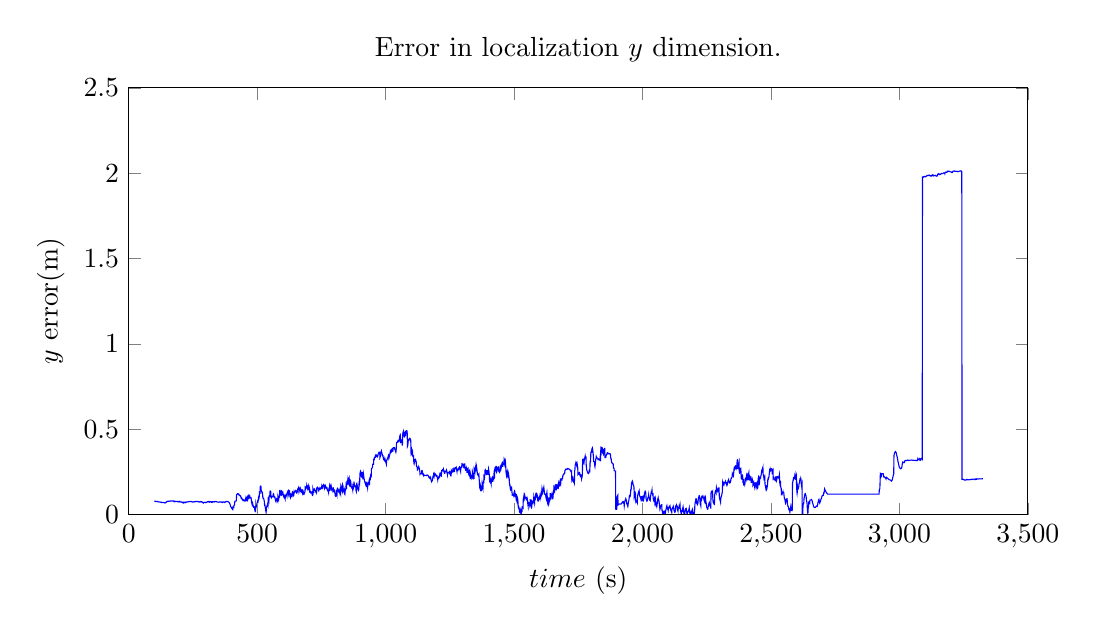
\begin{tikzpicture}

\begin{axis}[
title={Error in localization $y$ dimension.},
xlabel={$time$ (s)},
ylabel={$y$ error(m)},
xmin=0, xmax=3500,
ymin=0, ymax=2.5,
axis on top,
width=13cm,
height=7cm
]
\addplot [blue]
coordinates {
(100,0.0774476032257079)
(101,0.0782300930023192)
(102,0.0775148372650145)
(103,0.0775904159545897)
(104,0.0775258045196532)
(105,0.0764170627593992)
(106,0.0765572528839109)
(107,0.0767448883056638)
(108,0.07690234375)
(109,0.0761527557373047)
(110,0.0763685245513916)
(111,0.0760399837493897)
(112,0.0764589710235595)
(113,0.0763492984771728)
(114,0.0760431690216063)
(115,0.0739613513946531)
(116,0.0740390758514402)
(117,0.0735147933959959)
(118,0.0732394199371336)
(119,0.0741289653778074)
(120,0.0738211669921873)
(121,0.073763946533203)
(122,0.0739403762817381)
(123,0.0729645290374754)
(124,0.0724369087219237)
(125,0.0717807807922362)
(126,0.0704619045257568)
(127,0.0703648681640625)
(128,0.0701555366516113)
(129,0.0713868312835695)
(130,0.0709257297515871)
(131,0.0710418395996095)
(132,0.0705638103485109)
(133,0.0702010631561278)
(134,0.0703639030456542)
(135,0.0702103614807128)
(136,0.0701748371124267)
(137,0.0701021194458007)
(138,0.0699209213256835)
(139,0.0696352958679198)
(140,0.0694604816436768)
(141,0.0677605571746827)
(142,0.0681441726684571)
(143,0.0685010852813721)
(144,0.0700269451141358)
(145,0.070595573425293)
(146,0.0717316379547119)
(147,0.0747085514068604)
(148,0.0756343307495118)
(149,0.0763998928070069)
(150,0.0772157611846924)
(151,0.0762085456848145)
(152,0.0768727798461915)
(153,0.0775134105682374)
(154,0.0778121490478516)
(155,0.0775978107452393)
(156,0.0780889530181885)
(157,0.0780944366455079)
(158,0.0779099407196044)
(159,0.0783097686767578)
(160,0.0781607570648193)
(161,0.0789408950805663)
(162,0.0789191989898681)
(163,0.0790753631591796)
(164,0.0790055065155029)
(165,0.0787838993072509)
(166,0.0789465007781982)
(167,0.0790001449584961)
(168,0.0795885620117187)
(169,0.0794347820281982)
(170,0.0793572959899902)
(171,0.0790149269104004)
(172,0.0792120990753173)
(173,0.0791195926666259)
(174,0.0788523254394531)
(175,0.0792037544250488)
(176,0.0758047332763669)
(177,0.0750386943817136)
(178,0.0748899211883542)
(179,0.0778994789123533)
(180,0.0783560504913328)
(181,0.0767317047119138)
(182,0.0763244857788083)
(183,0.0761802444458008)
(184,0.0765495548248292)
(185,0.0768776187896729)
(186,0.0763647804260255)
(187,0.076724452972412)
(188,0.0766605567932128)
(189,0.0771404933929443)
(190,0.0750459098815917)
(191,0.0747993850708006)
(192,0.0748060607910155)
(193,0.0740834255218505)
(194,0.0742379207611084)
(195,0.0737494010925293)
(196,0.0736344833374023)
(197,0.0774712944030762)
(198,0.077686824798584)
(199,0.0772326374053955)
(200,0.0740206508636474)
(201,0.0737316875457763)
(202,0.0736325054168701)
(203,0.0735042362213134)
(204,0.0743115692138669)
(205,0.0740187911987302)
(206,0.0740991382598875)
(207,0.0715942649841308)
(208,0.0711438922882079)
(209,0.0709939270019531)
(210,0.0714180736541747)
(211,0.0678293533325194)
(212,0.0676798648834227)
(213,0.0677475757598875)
(214,0.0676045246124266)
(215,0.0727293338775632)
(216,0.0724229660034177)
(217,0.0723085250854489)
(218,0.0696561794281005)
(219,0.069549367904663)
(220,0.0693328838348388)
(221,0.0722963523864744)
(222,0.0730557155609128)
(223,0.0730838489532468)
(224,0.0736174297332761)
(225,0.0723216876983641)
(226,0.072814498901367)
(227,0.0731327877044676)
(228,0.0742109107971189)
(229,0.0744605350494383)
(230,0.0746009635925291)
(231,0.0744217166900634)
(232,0.0744994411468505)
(233,0.0746136436462401)
(234,0.074758840560913)
(235,0.0756670417785643)
(236,0.0757116260528563)
(237,0.0757607402801512)
(238,0.0759598102569581)
(239,0.0760189380645753)
(240,0.0760711517333985)
(241,0.0760914173126221)
(242,0.0761808242797852)
(243,0.0763577308654786)
(244,0.0765000667572022)
(245,0.0757722320556642)
(246,0.0748884143829347)
(247,0.0746764602661134)
(248,0.0723277645111082)
(249,0.0723353939056395)
(250,0.0729490833282469)
(251,0.0730461196899412)
(252,0.0733684616088865)
(253,0.0746866779327391)
(254,0.0751298980712889)
(255,0.0747372226715086)
(256,0.0746790485382078)
(257,0.0751589851379393)
(258,0.0745860652923582)
(259,0.0760702915191649)
(260,0.0754449195861815)
(261,0.0761534996032713)
(262,0.0760643310546874)
(263,0.0762464828491209)
(264,0.0764334030151366)
(265,0.0762429065704344)
(266,0.0766706409454345)
(267,0.076500410079956)
(268,0.076530927658081)
(269,0.0759815311431886)
(270,0.0762609577178956)
(271,0.0758282279968263)
(272,0.0757769680023195)
(273,0.0728068733215332)
(274,0.0725961112976075)
(275,0.0725248241424561)
(276,0.0733038253784177)
(277,0.0732666320800779)
(278,0.0731462306976316)
(279,0.0760299301147462)
(280,0.075494203567505)
(281,0.0753776168823244)
(282,0.0751455078125001)
(283,0.0751099834442139)
(284,0.0749097118377686)
(285,0.0746028671264649)
(286,0.0715063800811766)
(287,0.0708488216400145)
(288,0.0704256286621092)
(289,0.0685657062530516)
(290,0.0674541988372801)
(291,0.0670271911621092)
(292,0.0707690525054931)
(293,0.0710379886627197)
(294,0.0714230346679687)
(295,0.0715915966033935)
(296,0.0714342403411865)
(297,0.0716671752929687)
(298,0.0718021202087402)
(299,0.0693139209747313)
(300,0.0692149772644042)
(301,0.0693360939025878)
(302,0.0697447433471678)
(303,0.0718438091278077)
(304,0.0723936023712159)
(305,0.0726725521087648)
(306,0.0731536808013917)
(307,0.0756673622131347)
(308,0.075902681350708)
(309,0.076062421798706)
(310,0.0763811874389648)
(311,0.076351146697998)
(312,0.0764105129241943)
(313,0.0721520233154296)
(314,0.0723229694366454)
(315,0.0724498081207274)
(316,0.0748299388885498)
(317,0.0752064018249512)
(318,0.0749157695770264)
(319,0.075438766479492)
(320,0.075535087585449)
(321,0.0756557273864744)
(322,0.0718886947631834)
(323,0.0716562366485594)
(324,0.0715472793579099)
(325,0.0718069171905515)
(326,0.0754865741729738)
(327,0.0755099391937257)
(328,0.0757378673553468)
(329,0.0739039344787598)
(330,0.0739363594055176)
(331,0.0735107822418213)
(332,0.0733188552856445)
(333,0.0748991813659665)
(334,0.0746025886535642)
(335,0.0746362056732175)
(336,0.0762654399871825)
(337,0.0757683372497557)
(338,0.0758906459808348)
(339,0.0763655757904051)
(340,0.0754611701965331)
(341,0.0754857273101806)
(342,0.0758033008575438)
(343,0.073751630783081)
(344,0.0736121559143066)
(345,0.0729753398895263)
(346,0.0729195499420165)
(347,0.0727066421508789)
(348,0.072587194442749)
(349,0.0725349807739257)
(350,0.0722686672210693)
(351,0.0719878101348876)
(352,0.0722340965270996)
(353,0.0733169250488279)
(354,0.0733574562072752)
(355,0.0732604198455808)
(356,0.0732601814270017)
(357,0.0741257801055908)
(358,0.0742221012115478)
(359,0.0735297355651854)
(360,0.0734636936187743)
(361,0.0730729255676268)
(362,0.0732693824768065)
(363,0.0707930889129638)
(364,0.0705334510803222)
(365,0.0703286495208739)
(366,0.0730429992675781)
(367,0.0732895240783691)
(368,0.0730229721069335)
(369,0.073541955947876)
(370,0.0733485984802247)
(371,0.0735462474822999)
(372,0.0712923889160155)
(373,0.0723116283416747)
(374,0.0721866970062255)
(375,0.0716297512054442)
(376,0.0733675518035888)
(377,0.0744099178314208)
(378,0.0755035438537597)
(379,0.0759384193420409)
(380,0.0759152927398681)
(381,0.0771648445129394)
(382,0.0771021404266357)
(383,0.0762228450775146)
(384,0.0760306797027588)
(385,0.0768060169219971)
(386,0.0763213119506836)
(387,0.0753545646667479)
(388,0.0742142086029052)
(389,0.0736148242950438)
(390,0.0711011447906493)
(391,0.0700552024841308)
(392,0.0682034053802489)
(393,0.0640313396453855)
(394,0.0621847877502439)
(395,0.0585810909271238)
(396,0.0508472957611081)
(397,0.0474705734252927)
(398,0.0450906791687009)
(399,0.0427327194213865)
(400,0.0408761539459226)
(401,0.0369248428344724)
(402,0.0352435150146482)
(403,0.0329148807525632)
(404,0.0311713256835935)
(405,0.0292835273742673)
(406,0.0432978668212889)
(407,0.0414868392944334)
(408,0.0402260818481444)
(409,0.0402129688262938)
(410,0.0554012222290039)
(411,0.055361644744873)
(412,0.0570527477264404)
(413,0.0760257186889648)
(414,0.0777838172912597)
(415,0.0784437599182128)
(416,0.0786938610076904)
(417,0.0787947120666503)
(418,0.0799598636627197)
(419,0.0811207237243652)
(420,0.116963417053223)
(421,0.118111402511597)
(422,0.118822366714478)
(423,0.119765073776245)
(424,0.122234365463257)
(425,0.12197067451477)
(426,0.122261545181274)
(427,0.119364639282226)
(428,0.119584938049316)
(429,0.119540115356445)
(430,0.111603929519653)
(431,0.111579849243164)
(432,0.111283971786499)
(433,0.1106998462677)
(434,0.110586120605469)
(435,0.108918382644653)
(436,0.107568933486939)
(437,0.0977614688873292)
(438,0.0955744552612305)
(439,0.0981868076324464)
(440,0.0974517250061036)
(441,0.0932133579254151)
(442,0.0875034713745118)
(443,0.0858800792694092)
(444,0.088359064102173)
(445,0.0887033405303956)
(446,0.0830552043914796)
(447,0.0844894504547118)
(448,0.0815945720672606)
(449,0.0804747200012206)
(450,0.0796853160858153)
(451,0.0846993465423584)
(452,0.0851518650054932)
(453,0.0824708480834961)
(454,0.0881345806121825)
(455,0.0823879776000975)
(456,0.0817544994354247)
(457,0.0984533329010011)
(458,0.0946648616790773)
(459,0.0894065399169923)
(460,0.0937817592620851)
(461,0.0817270889282224)
(462,0.0803392543792723)
(463,0.0828643455505369)
(464,0.109322422027588)
(465,0.111979120254516)
(466,0.105591648101806)
(467,0.100411527633667)
(468,0.0968494453430173)
(469,0.100272659301758)
(470,0.107120517730713)
(471,0.1098521900177)
(472,0.101959104537964)
(473,0.0967053127288819)
(474,0.0961277484893799)
(475,0.0981476306915283)
(476,0.0987081527709961)
(477,0.0915126800537109)
(478,0.0747316112518308)
(479,0.0683677425384519)
(480,0.0617022743225095)
(481,0.0727243270874021)
(482,0.0701975669860837)
(483,0.0588655319213864)
(484,0.0550987567901609)
(485,0.049373611450195)
(486,0.0438332405090329)
(487,0.0451023426055905)
(488,0.0460965480804441)
(489,0.0453069057464597)
(490,0.0383961048126218)
(491,0.0252969112396237)
(492,0.0275930538177489)
(493,0.0230175628662108)
(494,0.0204507484436034)
(495,0.0620451946258544)
(496,0.0539225120544433)
(497,0.0468688983917236)
(498,0.0499361820220945)
(499,0.0512195892333982)
(500,0.0558136768341062)
(501,0.0618041820526121)
(502,0.0806722240447999)
(503,0.0826799468994142)
(504,0.080170114517212)
(505,0.100203443527222)
(506,0.103113103866577)
(507,0.108576465606689)
(508,0.103971887588501)
(509,0.128421096801758)
(510,0.126625089645386)
(511,0.125401763916015)
(512,0.16274587059021)
(513,0.166595376968384)
(514,0.166795886993408)
(515,0.161020435333252)
(516,0.137968727111816)
(517,0.134921499252319)
(518,0.13396854019165)
(519,0.127133228302002)
(520,0.129179098129272)
(521,0.124947406768799)
(522,0.101330055236816)
(523,0.0959029331207275)
(524,0.0964000358581543)
(525,0.0951628818511963)
(526,0.0899533309936524)
(527,0.0836392917633058)
(528,0.0742546596527101)
(529,0.0551449203491212)
(530,0.0561462783813478)
(531,0.0495180034637452)
(532,0.0402780914306642)
(533,0.0274846191406248)
(534,0.0185250873565672)
(535,0.0122258300781248)
(536,0.0422347908020018)
(537,0.0437320594787596)
(538,0.0491827850341795)
(539,0.0505403404235838)
(540,0.0576786117553709)
(541,0.0543185787200926)
(542,0.0499626712799071)
(543,0.0980168380737303)
(544,0.0998114147186278)
(545,0.0930496253967283)
(546,0.0851369895935057)
(547,0.107292108535767)
(548,0.106487445831299)
(549,0.106391839981079)
(550,0.134634998321533)
(551,0.1376107006073)
(552,0.136536148071289)
(553,0.134661462783813)
(554,0.100057641983032)
(555,0.0983794136047362)
(556,0.10739831161499)
(557,0.106701890945434)
(558,0.104345838546753)
(559,0.103618661880493)
(560,0.106154003143311)
(561,0.105690755844116)
(562,0.105391063690186)
(563,0.122012773513794)
(564,0.120304027557373)
(565,0.113169589996338)
(566,0.101997056961059)
(567,0.099962532043457)
(568,0.100539266586304)
(569,0.101611911773682)
(570,0.09516987991333)
(571,0.0869620819091796)
(572,0.0798574466705322)
(573,0.0762191791534423)
(574,0.0881618442535399)
(575,0.0897196712493895)
(576,0.0928174438476561)
(577,0.0896237297058105)
(578,0.0868969364166259)
(579,0.0794728202819823)
(580,0.076134006500244)
(581,0.108404165267944)
(582,0.102370983123779)
(583,0.0968706665039063)
(584,0.090888505935669)
(585,0.0994428234100342)
(586,0.100404842376709)
(587,0.103078706741333)
(588,0.139376150131226)
(589,0.138421998977661)
(590,0.13469384765625)
(591,0.116248821258545)
(592,0.114221309661865)
(593,0.11381671333313)
(594,0.139897584915161)
(595,0.13825535774231)
(596,0.129128456115723)
(597,0.122025966644287)
(598,0.127454393386841)
(599,0.126241081237793)
(600,0.129787557601929)
(601,0.121453834533691)
(602,0.113868309020996)
(603,0.104769302368164)
(604,0.101786849975586)
(605,0.105403898239136)
(606,0.108570335388184)
(607,0.0995041732788087)
(608,0.0956398849487305)
(609,0.090790927886963)
(610,0.111524560928345)
(611,0.111791589736939)
(612,0.114062049865723)
(613,0.118823268890381)
(614,0.117791999816895)
(615,0.110540975570679)
(616,0.106221784591675)
(617,0.127843683242798)
(618,0.129428689956665)
(619,0.133777683258057)
(620,0.129436647415161)
(621,0.125473892211914)
(622,0.119516288757324)
(623,0.140071823120117)
(624,0.137678577423096)
(625,0.13984294128418)
(626,0.138811065673828)
(627,0.114974563598633)
(628,0.104770009994507)
(629,0.100386922836304)
(630,0.121209264755249)
(631,0.120656610488892)
(632,0.115778566360474)
(633,0.113365293502808)
(634,0.104223358154297)
(635,0.103549348831177)
(636,0.104444372177124)
(637,0.133277320861816)
(638,0.132397317886352)
(639,0.130129480361938)
(640,0.117329772949219)
(641,0.114121850967407)
(642,0.110794004440308)
(643,0.114910778045654)
(644,0.13740927696228)
(645,0.135314292907715)
(646,0.130638904571533)
(647,0.131922817230225)
(648,0.134061193466187)
(649,0.137044525146484)
(650,0.139818159103394)
(651,0.136536804199219)
(652,0.135092226028442)
(653,0.129444328308105)
(654,0.133150903701782)
(655,0.138035861968994)
(656,0.136350004196167)
(657,0.142653783798218)
(658,0.135975917816162)
(659,0.13153942489624)
(660,0.151553647994995)
(661,0.152441757202149)
(662,0.159256952285767)
(663,0.155917184829712)
(664,0.150079284667969)
(665,0.143362794876098)
(666,0.137875591278076)
(667,0.152610372543335)
(668,0.15553862953186)
(669,0.150275300979614)
(670,0.144771032333374)
(671,0.137721471786499)
(672,0.132930212020874)
(673,0.130876712799072)
(674,0.144904865264893)
(675,0.145474924087524)
(676,0.141387714385986)
(677,0.122328639984131)
(678,0.116315961837769)
(679,0.116759658813477)
(680,0.131408868789673)
(681,0.126717983245849)
(682,0.124774633407593)
(683,0.121837793350219)
(684,0.127209287643433)
(685,0.128481489181519)
(686,0.132244688034058)
(687,0.158396886825562)
(688,0.15590016746521)
(689,0.153208898544312)
(690,0.159347429275513)
(691,0.156555309295654)
(692,0.156145467758179)
(693,0.169369873046875)
(694,0.159989055633545)
(695,0.153208908081055)
(696,0.149998601913452)
(697,0.165232954025269)
(698,0.166556415557861)
(699,0.170394954681397)
(700,0.15736622428894)
(701,0.153852649688721)
(702,0.145331331253052)
(703,0.140688844680786)
(704,0.151526123046875)
(705,0.142671733856201)
(706,0.135814100265503)
(707,0.130676052093506)
(708,0.126734039306641)
(709,0.12702610206604)
(710,0.132543584823608)
(711,0.131792566299438)
(712,0.130506059646606)
(713,0.127917072296142)
(714,0.117377540588379)
(715,0.113094589233398)
(716,0.112055561065674)
(717,0.15080905342102)
(718,0.144409183502197)
(719,0.136536840438843)
(720,0.148194536209107)
(721,0.147934659957886)
(722,0.148961051940918)
(723,0.150416484832764)
(724,0.148167720794678)
(725,0.143487802505493)
(726,0.131083400726318)
(727,0.131286294937134)
(728,0.13278666305542)
(729,0.135726186752319)
(730,0.133269760131836)
(731,0.129159900665283)
(732,0.155426462173462)
(733,0.155661542892456)
(734,0.156452854156494)
(735,0.159040410995483)
(736,0.155487306594849)
(737,0.150606163024902)
(738,0.144186742782593)
(739,0.150536514282226)
(740,0.151157594680786)
(741,0.146347499847412)
(742,0.153381603240967)
(743,0.14958597946167)
(744,0.148184555053711)
(745,0.148214834213257)
(746,0.154166954040527)
(747,0.15520932006836)
(748,0.153463380813599)
(749,0.157420623779297)
(750,0.152489412307739)
(751,0.1522982006073)
(752,0.167981338500976)
(753,0.163046312332153)
(754,0.161308479309082)
(755,0.157823514938354)
(756,0.167035753250122)
(757,0.166260654449463)
(758,0.17371576499939)
(759,0.1759049243927)
(760,0.173141414642334)
(761,0.163691455841064)
(762,0.156460458755493)
(763,0.166493528366089)
(764,0.168993347167969)
(765,0.161220424652099)
(766,0.164723655700683)
(767,0.156719705581665)
(768,0.155722877502441)
(769,0.154092809677124)
(770,0.157674095153808)
(771,0.159078857421875)
(772,0.155729553222656)
(773,0.147224208831787)
(774,0.140290996551514)
(775,0.138884803771973)
(776,0.140094301223755)
(777,0.133699676513672)
(778,0.12795760345459)
(779,0.147684642791748)
(780,0.145545074462891)
(781,0.144227573394776)
(782,0.167603265762329)
(783,0.176985513687134)
(784,0.173712741851807)
(785,0.16404701423645)
(786,0.150910627365112)
(787,0.143590700149536)
(788,0.144062530517578)
(789,0.162441570281982)
(790,0.155942279815674)
(791,0.146994668960571)
(792,0.140743572235107)
(793,0.150585645675659)
(794,0.150677198410034)
(795,0.154642576217651)
(796,0.155699247360229)
(797,0.149967664718628)
(798,0.13314532661438)
(799,0.132696298599243)
(800,0.138219026565552)
(801,0.140272764205933)
(802,0.131972570419312)
(803,0.124662656784058)
(804,0.110832710266113)
(805,0.108441133499146)
(806,0.106682796478272)
(807,0.108085651397705)
(808,0.114416856765747)
(809,0.144527383804321)
(810,0.131934829711914)
(811,0.12232417678833)
(812,0.150433038711548)
(813,0.154119228363037)
(814,0.152738069534302)
(815,0.141602491378784)
(816,0.14255478477478)
(817,0.133783603668213)
(818,0.131245637893677)
(819,0.129677320480347)
(820,0.138272071838379)
(821,0.142537857055664)
(822,0.131070638656616)
(823,0.142029813766479)
(824,0.134633354187012)
(825,0.126949361801147)
(826,0.170543413162231)
(827,0.167017202377319)
(828,0.159301500320435)
(829,0.147757511138916)
(830,0.141120891571045)
(831,0.135332565307617)
(832,0.131857614517212)
(833,0.171912546157837)
(834,0.166664953231812)
(835,0.151617164611817)
(836,0.13856255531311)
(837,0.134618396759033)
(838,0.133311862945557)
(839,0.128496522903442)
(840,0.141072797775268)
(841,0.132431316375732)
(842,0.125848579406738)
(843,0.140382759094238)
(844,0.142512075424194)
(845,0.149718753814697)
(846,0.168596185684204)
(847,0.161439336776733)
(848,0.148406423568725)
(849,0.18678465461731)
(850,0.183949142456055)
(851,0.19118180847168)
(852,0.187272459030151)
(853,0.201665868759155)
(854,0.189276208877563)
(855,0.185318222045898)
(856,0.209284021377564)
(857,0.206937744140625)
(858,0.212079002380371)
(859,0.18712780380249)
(860,0.173932765960693)
(861,0.165860866546631)
(862,0.165480827331543)
(863,0.198263488769531)
(864,0.19542702293396)
(865,0.182406507492065)
(866,0.165097831726074)
(867,0.158599494934082)
(868,0.156682371139526)
(869,0.154177783966065)
(870,0.15752255821228)
(871,0.152972339630127)
(872,0.144880174636841)
(873,0.169652578353882)
(874,0.165482160568237)
(875,0.157513257980347)
(876,0.164238569259644)
(877,0.192471700668335)
(878,0.179882961273193)
(879,0.169265466690063)
(880,0.170069686889648)
(881,0.167916767120361)
(882,0.162806741714477)
(883,0.164089195251465)
(884,0.157876483917236)
(885,0.140552751541138)
(886,0.136004917144775)
(887,0.179665557861328)
(888,0.181909791946411)
(889,0.173479072570801)
(890,0.165991924285889)
(891,0.154676578521729)
(892,0.147691390991211)
(893,0.144157908439636)
(894,0.140938661575317)
(895,0.144261620521545)
(896,0.147242687225342)
(897,0.1966132106781)
(898,0.181936401367187)
(899,0.179653901100159)
(900,0.238353047370911)
(901,0.245981607437134)
(902,0.236497077941894)
(903,0.242966333389282)
(904,0.233457723617554)
(905,0.225219884872436)
(906,0.222795167922974)
(907,0.243659280776978)
(908,0.247625373840332)
(909,0.246926449775696)
(910,0.227348589897156)
(911,0.216299319267273)
(912,0.208963298797607)
(913,0.209560537338257)
(914,0.233835701942444)
(915,0.223613624572754)
(916,0.210616593360901)
(917,0.206037612915039)
(918,0.195111008644104)
(919,0.192115398406982)
(920,0.186527701377869)
(921,0.188368650436401)
(922,0.183930965423584)
(923,0.172596188545227)
(924,0.173679571151733)
(925,0.163608174324036)
(926,0.16388557434082)
(927,0.192535590171814)
(928,0.180273126602173)
(929,0.165671538352966)
(930,0.156142543792725)
(931,0.172662049293518)
(932,0.180288702011108)
(933,0.18201318359375)
(934,0.185162454605102)
(935,0.192513110160828)
(936,0.184781672477722)
(937,0.171802045822143)
(938,0.204990166664123)
(939,0.217145341873169)
(940,0.219324726104736)
(941,0.2143773021698)
(942,0.228479103088379)
(943,0.225007251739502)
(944,0.22372599029541)
(945,0.268038820266724)
(946,0.26976210975647)
(947,0.271483968734741)
(948,0.272674988746643)
(949,0.278682520866394)
(950,0.294916561126709)
(951,0.295214465141296)
(952,0.293827822685242)
(953,0.293805530548096)
(954,0.323882596969604)
(955,0.323835747718811)
(956,0.323470848083496)
(957,0.335415698051453)
(958,0.334905363082886)
(959,0.335272885322571)
(960,0.335418082237244)
(961,0.349842573165894)
(962,0.349814558982849)
(963,0.349996949195862)
(964,0.340544979095459)
(965,0.341149131774902)
(966,0.341609518051147)
(967,0.343303362846374)
(968,0.338153288841248)
(969,0.34037368106842)
(970,0.343392417907715)
(971,0.354248385429382)
(972,0.356727223396301)
(973,0.358569841384888)
(974,0.365576672554016)
(975,0.36571352481842)
(976,0.365394639968872)
(977,0.365179109573364)
(978,0.333749332427979)
(979,0.337990798950195)
(980,0.342550554275513)
(981,0.364777987480164)
(982,0.366127555847168)
(983,0.366397326469421)
(984,0.371950333595276)
(985,0.363438108444214)
(986,0.355998375892639)
(987,0.352674224853516)
(988,0.344793670654297)
(989,0.345662587165833)
(990,0.344907634735107)
(991,0.331786029815674)
(992,0.322639527320862)
(993,0.322083535194397)
(994,0.322416009902954)
(995,0.318505945205688)
(996,0.324010910987854)
(997,0.329681577682495)
(998,0.324406685829163)
(999,0.317101302146912)
(1000,0.312287392616272)
(1001,0.304977653503418)
(1002,0.300889728546142)
(1003,0.294825075149536)
(1004,0.314526200294495)
(1005,0.319459438323975)
(1006,0.322843909263611)
(1007,0.326217889785767)
(1008,0.329703211784363)
(1009,0.334736108779907)
(1010,0.330048561096191)
(1011,0.342767465591431)
(1012,0.337803471565246)
(1013,0.342372644424438)
(1014,0.33727167892456)
(1015,0.345309422492981)
(1016,0.348107979774475)
(1017,0.358758018493652)
(1018,0.366044567108154)
(1019,0.361283586502075)
(1020,0.363804147720337)
(1021,0.377685354232788)
(1022,0.380433247566223)
(1023,0.376752064704895)
(1024,0.370664523124695)
(1025,0.37416331577301)
(1026,0.378827736854553)
(1027,0.373310611724853)
(1028,0.371893570899963)
(1029,0.37907271194458)
(1030,0.391575620651245)
(1031,0.391483352661133)
(1032,0.390217588424683)
(1033,0.392455742835998)
(1034,0.39203338432312)
(1035,0.386338994979858)
(1036,0.381707237243652)
(1037,0.379361317634582)
(1038,0.380222127914429)
(1039,0.369486139297485)
(1040,0.364913032531738)
(1041,0.371123002052307)
(1042,0.408173418998718)
(1043,0.421241737365723)
(1044,0.422411895751953)
(1045,0.422113276481628)
(1046,0.424740936279297)
(1047,0.429902340888977)
(1048,0.432286526679993)
(1049,0.430926109313965)
(1050,0.432183171272278)
(1051,0.434632206916809)
(1052,0.427926326751709)
(1053,0.430690909385681)
(1054,0.439389730453491)
(1055,0.454001689910889)
(1056,0.463407422065735)
(1057,0.466387415885925)
(1058,0.450171733856201)
(1059,0.422126794815064)
(1060,0.423063899040222)
(1061,0.432098890304565)
(1062,0.436549092292786)
(1063,0.436761284828186)
(1064,0.437591696739197)
(1065,0.40379598236084)
(1066,0.417854929924011)
(1067,0.474475766181946)
(1068,0.483335877418518)
(1069,0.482808137893677)
(1070,0.487941051483154)
(1071,0.475720532417297)
(1072,0.461032994270325)
(1073,0.458097584724426)
(1074,0.466687460899353)
(1075,0.475787182807922)
(1076,0.480016132354736)
(1077,0.47434677696228)
(1078,0.469410677909851)
(1079,0.480990310668945)
(1080,0.489383598327637)
(1081,0.490599533081055)
(1082,0.489843626976013)
(1083,0.490253587722778)
(1084,0.485896368980408)
(1085,0.398531360626221)
(1086,0.402326030731201)
(1087,0.413366360664368)
(1088,0.432537598609924)
(1089,0.435970349311829)
(1090,0.432935161590576)
(1091,0.433984680175781)
(1092,0.441378517150879)
(1093,0.445938868522644)
(1094,0.446996254920959)
(1095,0.446291131973267)
(1096,0.443529410362244)
(1097,0.439859910011291)
(1098,0.431820197105408)
(1099,0.365823216438294)
(1100,0.372663445472717)
(1101,0.378154582977295)
(1102,0.350827593803406)
(1103,0.348711152076721)
(1104,0.357130069732666)
(1105,0.363643546104431)
(1106,0.342133250236511)
(1107,0.337090578079223)
(1108,0.335757579803467)
(1109,0.338323559761047)
(1110,0.302927269935608)
(1111,0.297392740249634)
(1112,0.304098858833313)
(1113,0.315586452484131)
(1114,0.319544677734375)
(1115,0.316683654785156)
(1116,0.321639423370361)
(1117,0.318397914886475)
(1118,0.316656863212585)
(1119,0.311672603607178)
(1120,0.284186487197876)
(1121,0.281450037956238)
(1122,0.282103424072266)
(1123,0.278349165916443)
(1124,0.261944912910461)
(1125,0.264272951126099)
(1126,0.271812819480896)
(1127,0.27478519821167)
(1128,0.275138892173767)
(1129,0.280784167289734)
(1130,0.276023663520813)
(1131,0.270491041183472)
(1132,0.262698568344116)
(1133,0.254520691871643)
(1134,0.237250109672546)
(1135,0.240834494590759)
(1136,0.239036699295044)
(1137,0.240142036437988)
(1138,0.239036966323853)
(1139,0.238831091880798)
(1140,0.238941598892212)
(1141,0.257612418174744)
(1142,0.257148574829102)
(1143,0.255908917427063)
(1144,0.240966857910156)
(1145,0.234476388931274)
(1146,0.233301342964172)
(1147,0.229179920196533)
(1148,0.23529930305481)
(1149,0.233141495704651)
(1150,0.231717779159546)
(1151,0.228522894859314)
(1152,0.228507040023804)
(1153,0.228264568328857)
(1154,0.229315325737)
(1155,0.22898356628418)
(1156,0.228919431686401)
(1157,0.228252366065979)
(1158,0.228095009803772)
(1159,0.22779305267334)
(1160,0.228271201133728)
(1161,0.231741176605225)
(1162,0.231327639579773)
(1163,0.230309949874878)
(1164,0.230144417762756)
(1165,0.229122794151306)
(1166,0.226913726806641)
(1167,0.22459975528717)
(1168,0.220177885055542)
(1169,0.216183062553406)
(1170,0.215707179069519)
(1171,0.217221143722534)
(1172,0.212393048286438)
(1173,0.210587027549744)
(1174,0.212183491706848)
(1175,0.217280523300171)
(1176,0.212895528793335)
(1177,0.204263941764832)
(1178,0.197159496307373)
(1179,0.192573276519775)
(1180,0.195618239402771)
(1181,0.199265931129456)
(1182,0.199219916343689)
(1183,0.203022096633911)
(1184,0.220065704345703)
(1185,0.21903144454956)
(1186,0.221388808250427)
(1187,0.237201400756836)
(1188,0.23440594291687)
(1189,0.226178475379944)
(1190,0.236121260643005)
(1191,0.230263792991638)
(1192,0.232598983764648)
(1193,0.231790863990784)
(1194,0.235970225334167)
(1195,0.233440127372742)
(1196,0.232130732536316)
(1197,0.22544718837738)
(1198,0.227176080703735)
(1199,0.228886137962341)
(1200,0.228388796806335)
(1201,0.219294709205627)
(1202,0.212988537788391)
(1203,0.203904789924622)
(1204,0.216718862533569)
(1205,0.217407534599304)
(1206,0.21646137046814)
(1207,0.214368412971496)
(1208,0.223378541946411)
(1209,0.222858312606812)
(1210,0.221532347679138)
(1211,0.235317601203918)
(1212,0.243258847236633)
(1213,0.242981685638428)
(1214,0.23916873550415)
(1215,0.230380269050598)
(1216,0.226406665802002)
(1217,0.225375863075256)
(1218,0.25709023475647)
(1219,0.257621431350708)
(1220,0.256466293334961)
(1221,0.262134971618652)
(1222,0.261669816970825)
(1223,0.259637775421143)
(1224,0.263272943496704)
(1225,0.267264462471008)
(1226,0.260334349632263)
(1227,0.255694724082947)
(1228,0.24725780582428)
(1229,0.2420118932724)
(1230,0.242102611541748)
(1231,0.24247883605957)
(1232,0.253273546218872)
(1233,0.253173768043518)
(1234,0.253875791549683)
(1235,0.254746572494507)
(1236,0.252901212692261)
(1237,0.260275022506714)
(1238,0.256127935409546)
(1239,0.248097163200378)
(1240,0.241007667541504)
(1241,0.232280355453491)
(1242,0.244219924926758)
(1243,0.24505534362793)
(1244,0.244526412010193)
(1245,0.247057992935181)
(1246,0.247831422805786)
(1247,0.245465595245361)
(1248,0.242798525810242)
(1249,0.25062963104248)
(1250,0.252770629882813)
(1251,0.250312057495117)
(1252,0.242552603721619)
(1253,0.232137526512146)
(1254,0.226433004379272)
(1255,0.226826037406921)
(1256,0.259201900482178)
(1257,0.256679789543152)
(1258,0.256863729476929)
(1259,0.253427620887756)
(1260,0.251059051513672)
(1261,0.249559994697571)
(1262,0.267922268867493)
(1263,0.269636379241943)
(1264,0.261664258003235)
(1265,0.254330144882202)
(1266,0.252041822433472)
(1267,0.251401906967163)
(1268,0.251634841918945)
(1269,0.271795625686645)
(1270,0.272977347373962)
(1271,0.274646039009094)
(1272,0.273068002700806)
(1273,0.270292810440063)
(1274,0.271965912818909)
(1275,0.275255016326904)
(1276,0.26625435256958)
(1277,0.259392189025879)
(1278,0.25133244895935)
(1279,0.264368238449097)
(1280,0.263928356170654)
(1281,0.264502825736999)
(1282,0.26181441783905)
(1283,0.269268671035767)
(1284,0.268287817001343)
(1285,0.267009774208069)
(1286,0.27464639377594)
(1287,0.277701608657837)
(1288,0.280301205635071)
(1289,0.277199856758118)
(1290,0.263085199356079)
(1291,0.257258249282837)
(1292,0.251515699386597)
(1293,0.275514191627502)
(1294,0.276606029510498)
(1295,0.274576610565185)
(1296,0.274576372146606)
(1297,0.29313779258728)
(1298,0.290719393730164)
(1299,0.292595867156982)
(1300,0.293610691070557)
(1301,0.2961519947052)
(1302,0.290139674186707)
(1303,0.279068111419678)
(1304,0.278767661094665)
(1305,0.273647145271301)
(1306,0.273937658309936)
(1307,0.293080554008484)
(1308,0.295214281082153)
(1309,0.276320919990539)
(1310,0.270143136978149)
(1311,0.260764941215515)
(1312,0.262461647033691)
(1313,0.271173581123352)
(1314,0.275839391708374)
(1315,0.26928049659729)
(1316,0.259270969390869)
(1317,0.24424809551239)
(1318,0.270234594345093)
(1319,0.270119199752808)
(1320,0.26732958316803)
(1321,0.269413184165955)
(1322,0.249413799285889)
(1323,0.238664697647095)
(1324,0.23450226688385)
(1325,0.251877480506897)
(1326,0.257428699493408)
(1327,0.259555154800415)
(1328,0.239941835403442)
(1329,0.224932670593262)
(1330,0.207317233085632)
(1331,0.232427324295044)
(1332,0.224480117797851)
(1333,0.224097217559814)
(1334,0.219278420448303)
(1335,0.220683665275574)
(1336,0.21163556098938)
(1337,0.215077252388)
(1338,0.250405649185181)
(1339,0.24369190120697)
(1340,0.233563760757446)
(1341,0.218254941940308)
(1342,0.211052912712097)
(1343,0.212661403656006)
(1344,0.21219589138031)
(1345,0.267409058570862)
(1346,0.263033958435059)
(1347,0.256358476638794)
(1348,0.250935526847839)
(1349,0.269637272834778)
(1350,0.277658389091492)
(1351,0.275230453491211)
(1352,0.287826047897339)
(1353,0.274512873649597)
(1354,0.252941595077515)
(1355,0.269063516616821)
(1356,0.258246704101563)
(1357,0.242656394004822)
(1358,0.235182090759277)
(1359,0.235416268348694)
(1360,0.230841015815735)
(1361,0.233434413909912)
(1362,0.237013076782226)
(1363,0.238752026557922)
(1364,0.211189527511597)
(1365,0.195611972808838)
(1366,0.164645725250244)
(1367,0.153791838645935)
(1368,0.149859362602234)
(1369,0.171672018051148)
(1370,0.165593536376953)
(1371,0.160221131324768)
(1372,0.15070715713501)
(1373,0.155907827377319)
(1374,0.145819383621216)
(1375,0.149116593360901)
(1376,0.183205063819885)
(1377,0.173938568115234)
(1378,0.158033783912659)
(1379,0.151435430526733)
(1380,0.186152289390564)
(1381,0.1887142162323)
(1382,0.187518666267395)
(1383,0.224817321777344)
(1384,0.22147207069397)
(1385,0.216691539764404)
(1386,0.229181454658508)
(1387,0.258633309364319)
(1388,0.262449675559998)
(1389,0.259465151786804)
(1390,0.257229274749756)
(1391,0.244759863853455)
(1392,0.23659831905365)
(1393,0.235380596160889)
(1394,0.256349063873291)
(1395,0.257564998626709)
(1396,0.251478172302246)
(1397,0.24205387878418)
(1398,0.236402523994446)
(1399,0.235580218315125)
(1400,0.240927112579346)
(1401,0.264906763076782)
(1402,0.257328032493591)
(1403,0.242993830680847)
(1404,0.228036521911621)
(1405,0.192553749084473)
(1406,0.191328277587891)
(1407,0.189301719665527)
(1408,0.206600079536438)
(1409,0.200332531929016)
(1410,0.193863282203674)
(1411,0.182721862792969)
(1412,0.205122878074646)
(1413,0.206935574531555)
(1414,0.214669038772583)
(1415,0.217674298286438)
(1416,0.202176971435547)
(1417,0.191026253700256)
(1418,0.218667404174805)
(1419,0.21812190246582)
(1420,0.217347399711609)
(1421,0.212806002616882)
(1422,0.237376510620117)
(1423,0.230928599357605)
(1424,0.226204573631287)
(1425,0.265149809837341)
(1426,0.2735571641922)
(1427,0.276864387512207)
(1428,0.270701148033142)
(1429,0.268607604980469)
(1430,0.253848779678345)
(1431,0.250550377845764)
(1432,0.280130197525024)
(1433,0.278956582069397)
(1434,0.277239968299866)
(1435,0.272902419090271)
(1436,0.264616688251495)
(1437,0.259140988349915)
(1438,0.266090293884277)
(1439,0.275929197311401)
(1440,0.277538284301758)
(1441,0.270991667747497)
(1442,0.255405947208404)
(1443,0.257116458415985)
(1444,0.248322150707245)
(1445,0.250676712989807)
(1446,0.253925583362579)
(1447,0.276836504459381)
(1448,0.271662523269653)
(1449,0.268584599018097)
(1450,0.281103577613831)
(1451,0.279014554023743)
(1452,0.291744019985199)
(1453,0.300981786251068)
(1454,0.304160459518433)
(1455,0.296184344768524)
(1456,0.27969531583786)
(1457,0.297510401725769)
(1458,0.294826941013336)
(1459,0.293191568374634)
(1460,0.294057445049286)
(1461,0.313789568424225)
(1462,0.303129933357239)
(1463,0.297005854129791)
(1464,0.318213813781738)
(1465,0.322890871047974)
(1466,0.317301385879517)
(1467,0.302082174301147)
(1468,0.271724139690399)
(1469,0.244607602596283)
(1470,0.235514914035797)
(1471,0.254758884906769)
(1472,0.253979494571686)
(1473,0.239220371246338)
(1474,0.252116121768951)
(1475,0.245435454368591)
(1476,0.222670413970947)
(1477,0.220249094486237)
(1478,0.24138897895813)
(1479,0.234623970985413)
(1480,0.220573129653931)
(1481,0.213158406257629)
(1482,0.182743646144867)
(1483,0.174077011585236)
(1484,0.175233593940735)
(1485,0.154137423992157)
(1486,0.149186960220337)
(1487,0.143505683898926)
(1488,0.14533429479599)
(1489,0.150439432621002)
(1490,0.164947466373444)
(1491,0.149119274139404)
(1492,0.131307379722595)
(1493,0.115474717140198)
(1494,0.117009212493896)
(1495,0.113452066898346)
(1496,0.112447788238525)
(1497,0.117081472396851)
(1498,0.117183217525482)
(1499,0.111553081989288)
(1500,0.127249872684479)
(1501,0.126582181453705)
(1502,0.13846287727356)
(1503,0.136342821598053)
(1504,0.116084692955017)
(1505,0.103200374126434)
(1506,0.123959001541138)
(1507,0.10864644908905)
(1508,0.0949285593032837)
(1509,0.101489793539047)
(1510,0.089484375)
(1511,0.0817892365455627)
(1512,0.103671188116074)
(1513,0.0994122574329376)
(1514,0.0930844197273255)
(1515,0.0836986849308014)
(1516,0.0520992615222931)
(1517,0.0386366584300995)
(1518,0.0362372734546662)
(1519,0.042176070690155)
(1520,0.0373854963779449)
(1521,0.016438069820404)
(1522,0.0137636666297912)
(1523,0.0110366349220276)
(1524,0.0101646785736084)
(1525,0.0226431350708008)
(1526,0.0281724791526795)
(1527,0.0181457858085632)
(1528,0.00372915077209474)
(1529,0.0212376012802124)
(1530,0.0177588953971863)
(1531,0.0178121819496155)
(1532,0.0435175876617432)
(1533,0.0420553367137909)
(1534,0.04347199010849)
(1535,0.0408681612014771)
(1536,0.0885750069618225)
(1537,0.0977697088718414)
(1538,0.10388031744957)
(1539,0.113793630361557)
(1540,0.106779296159744)
(1541,0.0974907467365265)
(1542,0.108436388492584)
(1543,0.101610583782196)
(1544,0.101868910312653)
(1545,0.0987130529880524)
(1546,0.099363861322403)
(1547,0.0911951043605805)
(1548,0.0858651974201202)
(1549,0.0863215725421906)
(1550,0.0866999428272247)
(1551,0.0955692331790924)
(1552,0.0896428029537201)
(1553,0.0693682029247284)
(1554,0.0576735332012177)
(1555,0.0481245412826538)
(1556,0.0716431024074554)
(1557,0.0707722487449646)
(1558,0.0676488163471222)
(1559,0.0608019115924835)
(1560,0.0590138349533081)
(1561,0.0517105672359467)
(1562,0.0583492431640625)
(1563,0.0860198442935944)
(1564,0.0855450932979584)
(1565,0.0744072501659393)
(1566,0.0586471750736237)
(1567,0.0439119532108307)
(1568,0.0397658541202545)
(1569,0.0430865182876587)
(1570,0.0795994631052017)
(1571,0.0771340063810348)
(1572,0.0718092254400253)
(1573,0.072020080447197)
(1574,0.067514014005661)
(1575,0.0730195460319519)
(1576,0.0804626313447952)
(1577,0.105025012969971)
(1578,0.0972869889736176)
(1579,0.0783362733125687)
(1580,0.0687472270727158)
(1581,0.0948577334880829)
(1582,0.0962102969884872)
(1583,0.0940553357601166)
(1584,0.113283103227615)
(1585,0.108729427576065)
(1586,0.104194691300392)
(1587,0.108022963523865)
(1588,0.123295459270477)
(1589,0.121917533993721)
(1590,0.115726474046707)
(1591,0.104023758411407)
(1592,0.0852889605760574)
(1593,0.0790814646482468)
(1594,0.078484971165657)
(1595,0.0983703383803368)
(1596,0.0973460102081299)
(1597,0.0922098183631897)
(1598,0.0998462758660316)
(1599,0.0957892484664917)
(1600,0.0926473609805107)
(1601,0.0950476027727127)
(1602,0.118621656537056)
(1603,0.117440098762512)
(1604,0.104223662853241)
(1605,0.117592733204365)
(1606,0.107968333959579)
(1607,0.109870400130749)
(1608,0.115522134900093)
(1609,0.155496814548969)
(1610,0.149897606372833)
(1611,0.144149945378304)
(1612,0.13595982760191)
(1613,0.146779422998428)
(1614,0.146271680831909)
(1615,0.152344462811947)
(1616,0.159017179310322)
(1617,0.14597286298871)
(1618,0.129591662585735)
(1619,0.11943816408515)
(1620,0.118789918333292)
(1621,0.117510553061962)
(1622,0.118287562936544)
(1623,0.111051689445972)
(1624,0.10684782242775)
(1625,0.0928032731115818)
(1626,0.0886926313340664)
(1627,0.121367020837963)
(1628,0.129266427204013)
(1629,0.110891550153494)
(1630,0.0937309147119522)
(1631,0.0665387749969959)
(1632,0.0576827653050423)
(1633,0.0551428214013577)
(1634,0.0940796721279621)
(1635,0.0956512044668198)
(1636,0.0901834990382195)
(1637,0.0781157563924789)
(1638,0.0866162724494934)
(1639,0.0822913668751717)
(1640,0.0857146478891373)
(1641,0.125430747389793)
(1642,0.11164736700058)
(1643,0.101481973648071)
(1644,0.088934041082859)
(1645,0.1176402541399)
(1646,0.11756149405241)
(1647,0.117772211372852)
(1648,0.123563182592392)
(1649,0.113688744187355)
(1650,0.0998055558204651)
(1651,0.0886402051448822)
(1652,0.111948505043983)
(1653,0.121151864528656)
(1654,0.125213250517845)
(1655,0.151580225467682)
(1656,0.143979411363602)
(1657,0.134460460186005)
(1658,0.132269482851028)
(1659,0.166134601831436)
(1660,0.165729588270187)
(1661,0.173472514748573)
(1662,0.172145468473434)
(1663,0.152484697580338)
(1664,0.145148960232735)
(1665,0.144709569692612)
(1666,0.17432387638092)
(1667,0.174927716135979)
(1668,0.16407196688652)
(1669,0.156247903585434)
(1670,0.157748239040375)
(1671,0.155439840555191)
(1672,0.154162870645523)
(1673,0.18427602994442)
(1674,0.189622641086578)
(1675,0.182645008444786)
(1676,0.171067983388901)
(1677,0.167326704740524)
(1678,0.166677803874016)
(1679,0.172538862705231)
(1680,0.198712086558342)
(1681,0.194708293557167)
(1682,0.188087215900421)
(1683,0.206024118423462)
(1684,0.204209320902824)
(1685,0.202214934587479)
(1686,0.201715343356133)
(1687,0.212071173191071)
(1688,0.211687840819359)
(1689,0.211044647097588)
(1690,0.229062985181808)
(1691,0.231117035746574)
(1692,0.232804845571518)
(1693,0.23283582508564)
(1694,0.23911652636528)
(1695,0.239774904370308)
(1696,0.239826000452042)
(1697,0.240382081985474)
(1698,0.25799520611763)
(1699,0.258683028817177)
(1700,0.262309613823891)
(1701,0.266329329848289)
(1702,0.266294803857803)
(1703,0.266324382662773)
(1704,0.266241725921631)
(1705,0.265118016600609)
(1706,0.264864950180054)
(1707,0.264680831432343)
(1708,0.270168567061424)
(1709,0.269976818919182)
(1710,0.269355783224106)
(1711,0.268622854709625)
(1712,0.268199184894562)
(1713,0.267268294453621)
(1714,0.265749685883522)
(1715,0.265234433531761)
(1716,0.264812253832817)
(1717,0.263859577894211)
(1718,0.261487664103508)
(1719,0.259596617341042)
(1720,0.257175223350525)
(1721,0.253116413593292)
(1722,0.249646722912788)
(1723,0.248775332808495)
(1724,0.251937582731247)
(1725,0.198335386037827)
(1726,0.201754129648209)
(1727,0.200209743499756)
(1728,0.204059062242508)
(1729,0.211296124100685)
(1730,0.202806008696556)
(1731,0.19470049226284)
(1732,0.190507961153984)
(1733,0.191832137942314)
(1734,0.18750358903408)
(1735,0.182798860311508)
(1736,0.258063789486885)
(1737,0.262033965468407)
(1738,0.28841709458828)
(1739,0.294060402750969)
(1740,0.298810699224472)
(1741,0.305911698579788)
(1742,0.302970169901848)
(1743,0.295945613503456)
(1744,0.285304277062416)
(1745,0.281555010795593)
(1746,0.293964609265327)
(1747,0.285183667898178)
(1748,0.274017423152924)
(1749,0.236114999294281)
(1750,0.238863965511322)
(1751,0.241114547491074)
(1752,0.237500688076019)
(1753,0.236631920576096)
(1754,0.244335567593575)
(1755,0.245645036935806)
(1756,0.238784075260162)
(1757,0.227122515916824)
(1758,0.224774092912674)
(1759,0.227927357435226)
(1760,0.223729312896729)
(1761,0.220430255413055)
(1762,0.234461308002472)
(1763,0.209226428508759)
(1764,0.214356972813606)
(1765,0.222967623710632)
(1766,0.228186606407166)
(1767,0.323268898844719)
(1768,0.324045115232468)
(1769,0.314167150378227)
(1770,0.308346890926361)
(1771,0.319998507261276)
(1772,0.322245512962341)
(1773,0.312735442876816)
(1774,0.325614061355591)
(1775,0.330845322608948)
(1776,0.336083050966263)
(1777,0.34350721180439)
(1778,0.336388899564743)
(1779,0.335932789921761)
(1780,0.336459978103638)
(1781,0.288740883708)
(1782,0.273864443540573)
(1783,0.261587078809738)
(1784,0.255642618179321)
(1785,0.253892953634262)
(1786,0.248555894136429)
(1787,0.243181104898453)
(1788,0.242039824962616)
(1789,0.247331257104874)
(1790,0.247276867866516)
(1791,0.243623162746429)
(1792,0.247241611719132)
(1793,0.25931381726265)
(1794,0.262906069993973)
(1795,0.247485871553421)
(1796,0.308580920696259)
(1797,0.306894228458405)
(1798,0.312195048332214)
(1799,0.365915012836456)
(1800,0.366243911266327)
(1801,0.368236881971359)
(1802,0.366674286603928)
(1803,0.385641190052032)
(1804,0.386990877628326)
(1805,0.390512856483459)
(1806,0.382589509725571)
(1807,0.370807429790497)
(1808,0.356380751371384)
(1809,0.339574208498001)
(1810,0.312176874637604)
(1811,0.312006286144257)
(1812,0.308661988735199)
(1813,0.301097714424133)
(1814,0.286954068660736)
(1815,0.280051314353943)
(1816,0.291974150657654)
(1817,0.307579153299332)
(1818,0.32357882809639)
(1819,0.325900011777878)
(1820,0.339647376060486)
(1821,0.335794203996658)
(1822,0.333307677030563)
(1823,0.331513785839081)
(1824,0.331387722015381)
(1825,0.330550843000412)
(1826,0.329203330993652)
(1827,0.320433331727982)
(1828,0.320513172149658)
(1829,0.322068734169006)
(1830,0.32440770983696)
(1831,0.323539597988129)
(1832,0.322312219142914)
(1833,0.320303393602371)
(1834,0.318392736911774)
(1835,0.331199182271957)
(1836,0.321650458574295)
(1837,0.313433570861816)
(1838,0.39875340628624)
(1839,0.382184536933899)
(1840,0.373790206193924)
(1841,0.389689151763916)
(1842,0.387606416463852)
(1843,0.387739334821701)
(1844,0.388981078386307)
(1845,0.366933550357819)
(1846,0.37065958571434)
(1847,0.37392302942276)
(1848,0.376377071857452)
(1849,0.35462303185463)
(1850,0.358511489868164)
(1851,0.360554468870163)
(1852,0.362796229362488)
(1853,0.390591963291168)
(1854,0.334103985786438)
(1855,0.334409966230392)
(1856,0.333954974174499)
(1857,0.333928301095962)
(1858,0.342162950992584)
(1859,0.346746071338654)
(1860,0.350873663187027)
(1861,0.353949888706207)
(1862,0.355560167789459)
(1863,0.36157635307312)
(1864,0.361749444961548)
(1865,0.362452422142029)
(1866,0.355289520263672)
(1867,0.355831833124161)
(1868,0.356164665460587)
(1869,0.355901630163193)
(1870,0.356282980680466)
(1871,0.356465907335281)
(1872,0.356937052249908)
(1873,0.356938482761383)
(1874,0.354936321020126)
(1875,0.354617853403091)
(1876,0.33977930688858)
(1877,0.326959361076355)
(1878,0.326828439474106)
(1879,0.314835120677948)
(1880,0.303319264888763)
(1881,0.30256195807457)
(1882,0.301834960222244)
(1883,0.300852616071701)
(1884,0.298394043207169)
(1885,0.297429491043091)
(1886,0.296332080125809)
(1887,0.273838042259216)
(1888,0.272803454637528)
(1889,0.272109835386276)
(1890,0.25736633348465)
(1891,0.256748352527618)
(1892,0.25591010260582)
(1893,0.255114142179489)
(1894,0.254798923015594)
(1895,0.254230652332306)
(1896,0.0314550061225891)
(1897,0.0298494753837585)
(1898,0.0300844368934631)
(1899,0.0309402403831481)
(1900,0.0312808213233947)
(1901,0.102573867797852)
(1902,0.107022579669952)
(1903,0.110068496227264)
(1904,0.113006289958954)
(1905,0.0559926733970642)
(1906,0.0571524009704589)
(1907,0.0594991550445556)
(1908,0.0599547729492187)
(1909,0.0608875260353088)
(1910,0.0616690025329589)
(1911,0.0619146928787231)
(1912,0.0609916553497314)
(1913,0.0607957944869995)
(1914,0.0610209808349609)
(1915,0.0615516719818116)
(1916,0.0617753682136536)
(1917,0.061665397644043)
(1918,0.062792163848877)
(1919,0.0658224215507507)
(1920,0.0683763613700866)
(1921,0.0706667890548706)
(1922,0.0725735425949097)
(1923,0.0755705833435059)
(1924,0.0764967203140259)
(1925,0.069037139415741)
(1926,0.0673060417175293)
(1927,0.0699557662010193)
(1928,0.0654403567314148)
(1929,0.0499887495040894)
(1930,0.0613067774772644)
(1931,0.0745008020401001)
(1932,0.0812922744750977)
(1933,0.0848398237228394)
(1934,0.0847137002944947)
(1935,0.092740538597107)
(1936,0.0897652277946472)
(1937,0.0826246509552002)
(1938,0.0742723712921143)
(1939,0.0625495085716248)
(1940,0.0600368747711182)
(1941,0.0574428210258484)
(1942,0.0520945558547974)
(1943,0.047567370891571)
(1944,0.0567740235328674)
(1945,0.071594539642334)
(1946,0.0757213268280029)
(1947,0.0828492069244384)
(1948,0.0954413437843322)
(1949,0.109526100158691)
(1950,0.111395301818848)
(1951,0.107839229106903)
(1952,0.106417598724365)
(1953,0.11266571521759)
(1954,0.142359860897064)
(1955,0.141378172397614)
(1956,0.147773154735565)
(1957,0.178752414703369)
(1958,0.185908786773682)
(1959,0.190559319972992)
(1960,0.194217316627502)
(1961,0.185430909156799)
(1962,0.188586975097656)
(1963,0.18124320602417)
(1964,0.172757233142853)
(1965,0.169204617500305)
(1966,0.167585457324982)
(1967,0.157035733222961)
(1968,0.0994051346778869)
(1969,0.10538586473465)
(1970,0.114604736328125)
(1971,0.102702214241028)
(1972,0.100578143119812)
(1973,0.11010010433197)
(1974,0.0775060391426087)
(1975,0.0815534925460816)
(1976,0.078980360031128)
(1977,0.0747961139678955)
(1978,0.0780443286895752)
(1979,0.0785654520988465)
(1980,0.0729133820533753)
(1981,0.107231077194214)
(1982,0.115667339801788)
(1983,0.122922894001007)
(1984,0.12655907535553)
(1985,0.129688438415527)
(1986,0.137540575504303)
(1987,0.140730139255524)
(1988,0.114977599620819)
(1989,0.110416592597961)
(1990,0.106056572437286)
(1991,0.104794742107391)
(1992,0.0975117697715759)
(1993,0.0962593569755554)
(1994,0.0896969661712647)
(1995,0.09819801902771)
(1996,0.103360615730286)
(1997,0.102493904590607)
(1998,0.0929942355155945)
(1999,0.105118356704712)
(2000,0.105901561737061)
(2001,0.0853649325370789)
(2002,0.0813669509887696)
(2003,0.0802849478721619)
(2004,0.0965518326759338)
(2005,0.0905250878334045)
(2006,0.0968693466186523)
(2007,0.10560732793808)
(2008,0.125684498310089)
(2009,0.12966751909256)
(2010,0.134456990718842)
(2011,0.128379164218903)
(2012,0.130842743396759)
(2013,0.126924214839935)
(2014,0.0916985468864441)
(2015,0.0901303486824035)
(2016,0.0827712016105652)
(2017,0.0785766439437866)
(2018,0.0789403576850891)
(2019,0.0841239352226257)
(2020,0.0927636284828186)
(2021,0.0981143374443054)
(2022,0.0983640213012695)
(2023,0.10519060087204)
(2024,0.114927913665771)
(2025,0.100670846939087)
(2026,0.0984371032714844)
(2027,0.0913870062828064)
(2028,0.0855781178474426)
(2029,0.0833924155235291)
(2030,0.0816436748504639)
(2031,0.102772013187408)
(2032,0.111404792308807)
(2033,0.120500580310822)
(2034,0.130143062114716)
(2035,0.129243048667908)
(2036,0.136423024177551)
(2037,0.143710288047791)
(2038,0.123178745746613)
(2039,0.120428110599518)
(2040,0.113849307537079)
(2041,0.116913045883179)
(2042,0.0908332328796386)
(2043,0.0842509131431579)
(2044,0.080617175579071)
(2045,0.0864070062637329)
(2046,0.094488561630249)
(2047,0.0975900297164917)
(2048,0.0761376686096191)
(2049,0.086644775390625)
(2050,0.0947691268920898)
(2051,0.0858880348205566)
(2052,0.052325662612915)
(2053,0.0497926440238953)
(2054,0.0536286201477051)
(2055,0.0599277930259704)
(2056,0.0510890202522277)
(2057,0.0607672052383422)
(2058,0.0673474388122558)
(2059,0.0836181631088256)
(2060,0.0927854766845703)
(2061,0.0980242481231689)
(2062,0.0866622419357299)
(2063,0.086446473121643)
(2064,0.0828388423919677)
(2065,0.0710638256072997)
(2066,0.0551363658905029)
(2067,0.0431661438941955)
(2068,0.0301196408271789)
(2069,0.0346633148193359)
(2070,0.044055278301239)
(2071,0.0492382597923279)
(2072,0.0524748516082764)
(2073,0.0512782917022705)
(2074,0.057179986000061)
(2075,0.057523904800415)
(2076,0.0240920028686523)
(2077,0.0227544150352478)
(2078,0.0117599210739135)
(2079,0.0138462028503418)
(2080,0.0114553623199463)
(2081,0.00142229127883908)
(2082,0.00388610887527463)
(2083,0.0188571329116821)
(2084,0.0192840213775635)
(2085,0.0176307077407837)
(2086,0.0186838622093201)
(2087,0.0103685913085937)
(2088,0.00773686742782587)
(2089,0.00202662324905389)
(2090,0.0190691533088684)
(2091,0.027863878250122)
(2092,0.0321499290466308)
(2093,0.0415995302200317)
(2094,0.046652198791504)
(2095,0.0513008246421814)
(2096,0.0404120693206788)
(2097,0.0345631847381592)
(2098,0.0336003332138062)
(2099,0.0292356042861939)
(2100,0.023198130607605)
(2101,0.0372709436416627)
(2102,0.0361478729248048)
(2103,0.0380280418395997)
(2104,0.0480662741661071)
(2105,0.0470419087409972)
(2106,0.0458944597244262)
(2107,0.0500037231445312)
(2108,0.0418975172042846)
(2109,0.0341737089157104)
(2110,0.0265301284790038)
(2111,0.0223530945777892)
(2112,0.023614164352417)
(2113,0.018582221031189)
(2114,0.0131292901039124)
(2115,0.0322818808555603)
(2116,0.0348089389801025)
(2117,0.0394020133018493)
(2118,0.0389132590293884)
(2119,0.0428658814430236)
(2120,0.0487715096473693)
(2121,0.0441780776977538)
(2122,0.0305175724029541)
(2123,0.0218906345367431)
(2124,0.021182650566101)
(2125,0.0158975067138671)
(2126,0.0188338012695313)
(2127,0.016518518447876)
(2128,0.0201032609939575)
(2129,0.0464319400787354)
(2130,0.0507847480773926)
(2131,0.049390118598938)
(2132,0.048305878162384)
(2133,0.0556344480514526)
(2134,0.0517318339347839)
(2135,0.0438366622924804)
(2136,0.0291546087265016)
(2137,0.0236024360656739)
(2138,0.0193824272155763)
(2139,0.0369037523269653)
(2140,0.0338752403259277)
(2141,0.0343886747360229)
(2142,0.0394228830337524)
(2143,0.0509643211364745)
(2144,0.0490446939468383)
(2145,0.0548743858337402)
(2146,0.0608124389648437)
(2147,0.0347775430679322)
(2148,0.0250021429061891)
(2149,0.0178820104599)
(2150,0.00975974464416507)
(2151,0.000749787330627472)
(2152,0.0063332710266113)
(2153,0.0209698610305786)
(2154,0.0255045824050903)
(2155,0.0279797248840332)
(2156,0.0248297386169434)
(2157,0.0398087396621705)
(2158,0.0452849760055543)
(2159,0.0353575839996338)
(2160,0.0190164566040039)
(2161,0.0100050687789917)
(2162,0.00267512798309322)
(2163,0.0092667446136474)
(2164,0.00389600849151606)
(2165,0.00716401195526117)
(2166,0.0277334947586059)
(2167,0.0303890008926391)
(2168,0.0278554458618163)
(2169,0.0357062120437621)
(2170,0.0364414796829224)
(2171,0.0285667524337769)
(2172,0.0216051683425904)
(2173,0.00361123752594006)
(2174,0.00317105579376209)
(2175,0.00736448097228992)
(2176,0.0134580869674683)
(2177,0.0145389575958252)
(2178,0.0180599231719971)
(2179,0.0215531129837037)
(2180,0.0261976003646851)
(2181,0.0301957607269288)
(2182,0.0376630306243897)
(2183,0.0205689430236817)
(2184,0.0111361503601075)
(2185,0.00474021434783944)
(2186,0.0011795997619628)
(2187,0.00288551425933825)
(2188,0.0116560993194579)
(2189,0.0164377031326293)
(2190,0.00757421493530286)
(2191,0.0112381124496461)
(2192,0.01271785736084)
(2193,0.011007113456726)
(2194,0.0220225286483764)
(2195,0.0295610857009887)
(2196,0.0240893793106078)
(2197,0.00127505588531496)
(2198,0.00498533916473387)
(2199,0.00865269374847411)
(2200,0.00769445705413818)
(2201,0.00284788417816162)
(2202,0.0131333808898926)
(2203,0.0187309722900391)
(2204,0.0609194927215577)
(2205,0.0633424215316774)
(2206,0.0768778018951417)
(2207,0.0787857866287232)
(2208,0.0931876993179321)
(2209,0.0931757783889771)
(2210,0.0741144666671754)
(2211,0.0656539449691773)
(2212,0.0638040552139283)
(2213,0.0607203493118287)
(2214,0.0688105487823487)
(2215,0.0635071659088136)
(2216,0.0683498048782349)
(2217,0.084810700416565)
(2218,0.0988480777740479)
(2219,0.100426170349121)
(2220,0.109083029747009)
(2221,0.110282857894898)
(2222,0.106358249664307)
(2223,0.0941210584640504)
(2224,0.0755531387329103)
(2225,0.0599379796981812)
(2226,0.0597192306518555)
(2227,0.0524024028778076)
(2228,0.0936257038116455)
(2229,0.0925187263488769)
(2230,0.0990946683883667)
(2231,0.0927451047897339)
(2232,0.0989772472381591)
(2233,0.102216282844543)
(2234,0.106958428382874)
(2235,0.109433557510376)
(2236,0.102775361061096)
(2237,0.098786379814148)
(2238,0.0957081575393677)
(2239,0.0923369188308716)
(2240,0.0820207853317261)
(2241,0.0781995315551758)
(2242,0.0997636213302613)
(2243,0.104158987045288)
(2244,0.107941855430603)
(2245,0.104018200874329)
(2246,0.0722045707702637)
(2247,0.075203161239624)
(2248,0.066498498916626)
(2249,0.0575412321090698)
(2250,0.0417689409255981)
(2251,0.0394720163345337)
(2252,0.0374056425094604)
(2253,0.0316334095001221)
(2254,0.0310800399780273)
(2255,0.0380708303451538)
(2256,0.0463965263366699)
(2257,0.0532723989486694)
(2258,0.061438473701477)
(2259,0.0663662281036377)
(2260,0.0705062475204468)
(2261,0.0631032314300537)
(2262,0.0564513530731201)
(2263,0.0503431882858276)
(2264,0.0476436939239502)
(2265,0.044152530670166)
(2266,0.0346925582885742)
(2267,0.130408390045166)
(2268,0.130585892677307)
(2269,0.135816677093506)
(2270,0.134717686653137)
(2271,0.129659755706787)
(2272,0.131498439788818)
(2273,0.134795291900635)
(2274,0.0848505201339722)
(2275,0.0736645164489746)
(2276,0.0691288414001465)
(2277,0.0660149755477906)
(2278,0.0670579376220704)
(2279,0.0605582895278931)
(2280,0.0595199766159058)
(2281,0.113158498764038)
(2282,0.120658908843994)
(2283,0.130985413551331)
(2284,0.136443291664124)
(2285,0.140866313934326)
(2286,0.142823968887329)
(2287,0.135229502677918)
(2288,0.157350004196167)
(2289,0.149863303184509)
(2290,0.147655666351318)
(2291,0.138593495368958)
(2292,0.139609939575195)
(2293,0.135665423393249)
(2294,0.142094738006592)
(2295,0.153869694709778)
(2296,0.155326670646668)
(2297,0.154733127593994)
(2298,0.155123776435852)
(2299,0.108221283912659)
(2300,0.0989301118850707)
(2301,0.0897574338912963)
(2302,0.0825945930480958)
(2303,0.0783581333160401)
(2304,0.0717243747711183)
(2305,0.0940646266937255)
(2306,0.100481662750244)
(2307,0.109026346206665)
(2308,0.110136542320251)
(2309,0.117847595214844)
(2310,0.126989278793335)
(2311,0.13207248210907)
(2312,0.186075083732605)
(2313,0.179319493293762)
(2314,0.179196826934815)
(2315,0.183585397720337)
(2316,0.176138035774231)
(2317,0.173357479095459)
(2318,0.180056445121765)
(2319,0.188221446990967)
(2320,0.187935583114624)
(2321,0.186869494438171)
(2322,0.189094058990479)
(2323,0.194171897888184)
(2324,0.188515536308289)
(2325,0.182744853019714)
(2326,0.179442771911621)
(2327,0.183105834960938)
(2328,0.177687653541565)
(2329,0.171045431137085)
(2330,0.174692520141602)
(2331,0.183161982536316)
(2332,0.189669498443604)
(2333,0.197891238212585)
(2334,0.19776010799408)
(2335,0.203076842308044)
(2336,0.197227297782898)
(2337,0.193619905471802)
(2338,0.189341364860535)
(2339,0.192681254386902)
(2340,0.193726362228394)
(2341,0.186280430793762)
(2342,0.187327445983887)
(2343,0.193401755332947)
(2344,0.203813137054443)
(2345,0.211939515113831)
(2346,0.211317123413086)
(2347,0.214912475585938)
(2348,0.218690337181091)
(2349,0.220476449966431)
(2350,0.241675251960754)
(2351,0.239002102851868)
(2352,0.236993426322937)
(2353,0.229680413246155)
(2354,0.226625317573547)
(2355,0.242836469650269)
(2356,0.259679907798767)
(2357,0.274442006111145)
(2358,0.277815509796143)
(2359,0.279345203399658)
(2360,0.26532275390625)
(2361,0.267010161399841)
(2362,0.278357216835022)
(2363,0.28524155330658)
(2364,0.284409591674805)
(2365,0.279267379760742)
(2366,0.273418852806091)
(2367,0.282173225402832)
(2368,0.302587935447693)
(2369,0.319270441055298)
(2370,0.320688316345215)
(2371,0.271606748580933)
(2372,0.272609894752502)
(2373,0.270914977073669)
(2374,0.279992764472961)
(2375,0.296545808792114)
(2376,0.304230278015137)
(2377,0.248036720275879)
(2378,0.245044805526733)
(2379,0.249998547554016)
(2380,0.264105774879456)
(2381,0.260823389053345)
(2382,0.27014984703064)
(2383,0.270917674064636)
(2384,0.219827095985413)
(2385,0.210235039710999)
(2386,0.208858291625977)
(2387,0.219643394470215)
(2388,0.231284777641297)
(2389,0.231384973049164)
(2390,0.224916438579559)
(2391,0.184704915046692)
(2392,0.195347145557404)
(2393,0.206579342842102)
(2394,0.179144425868988)
(2395,0.1819182472229)
(2396,0.184030039787292)
(2397,0.179865940093994)
(2398,0.174622287273407)
(2399,0.185221065998077)
(2400,0.207303812026977)
(2401,0.211543684005737)
(2402,0.210419659614563)
(2403,0.205975716114044)
(2404,0.21756959438324)
(2405,0.226914649009705)
(2406,0.234008495807648)
(2407,0.244341259002686)
(2408,0.208204926967621)
(2409,0.21131795835495)
(2410,0.20468098115921)
(2411,0.204372825145722)
(2412,0.221374202728271)
(2413,0.238326419353485)
(2414,0.244912136554718)
(2415,0.208687928676605)
(2416,0.206473020076752)
(2417,0.212837246417999)
(2418,0.219391432762146)
(2419,0.210832717895508)
(2420,0.215405169010162)
(2421,0.218726518630981)
(2422,0.219793143749237)
(2423,0.188502862453461)
(2424,0.188000812530518)
(2425,0.193600788116455)
(2426,0.204140407085419)
(2427,0.208515149593353)
(2428,0.202203434944153)
(2429,0.198595744609833)
(2430,0.173324436664581)
(2431,0.178110928058624)
(2432,0.18481275510788)
(2433,0.188386590003967)
(2434,0.174012627124786)
(2435,0.171379532337189)
(2436,0.167541291236877)
(2437,0.159214748382568)
(2438,0.168163312911987)
(2439,0.184763325691223)
(2440,0.18533070230484)
(2441,0.179418100357056)
(2442,0.181994809150696)
(2443,0.165400611877441)
(2444,0.175047981262207)
(2445,0.178875672340393)
(2446,0.182568418502808)
(2447,0.15823894071579)
(2448,0.154513352394104)
(2449,0.158814602375031)
(2450,0.204490758419037)
(2451,0.214518703460693)
(2452,0.223772026538849)
(2453,0.222177006244659)
(2454,0.171590065956116)
(2455,0.181090986728668)
(2456,0.199757850170135)
(2457,0.210700272083282)
(2458,0.217831252574921)
(2459,0.219402132987976)
(2460,0.217259592533112)
(2461,0.225843257427216)
(2462,0.233003503799438)
(2463,0.240373141288757)
(2464,0.257782006263733)
(2465,0.259516382217407)
(2466,0.264462733268738)
(2467,0.24551539850235)
(2468,0.26114039850235)
(2469,0.269641153335571)
(2470,0.232566302776337)
(2471,0.230803555011749)
(2472,0.222145920753479)
(2473,0.209350087165833)
(2474,0.213220157146454)
(2475,0.21414599609375)
(2476,0.21968034696579)
(2477,0.179836196422577)
(2478,0.17093483877182)
(2479,0.163877529621124)
(2480,0.155571994781494)
(2481,0.166068730354309)
(2482,0.168263850212097)
(2483,0.168182311058044)
(2484,0.150551507949829)
(2485,0.155241320610046)
(2486,0.168792317390442)
(2487,0.17301208782196)
(2488,0.207227555751801)
(2489,0.210947004795074)
(2490,0.207958606719971)
(2491,0.211883091926575)
(2492,0.219835305213928)
(2493,0.229539239406586)
(2494,0.244428777694702)
(2495,0.258570521354675)
(2496,0.255955665588379)
(2497,0.265021293640137)
(2498,0.257449329853058)
(2499,0.261010349750519)
(2500,0.261323989391327)
(2501,0.264190257549286)
(2502,0.267885209083557)
(2503,0.26641178226471)
(2504,0.262812973022461)
(2505,0.235140823841095)
(2506,0.246346139431)
(2507,0.260326349258423)
(2508,0.263316654682159)
(2509,0.213016729831696)
(2510,0.216141860961914)
(2511,0.219662647724152)
(2512,0.218689005851746)
(2513,0.203639574527741)
(2514,0.20433229970932)
(2515,0.203653760433197)
(2516,0.205221541404724)
(2517,0.201106973171234)
(2518,0.204531200408936)
(2519,0.223391153097153)
(2520,0.202557783126831)
(2521,0.204088668823242)
(2522,0.198546628952026)
(2523,0.207017432451248)
(2524,0.222078512907028)
(2525,0.222385178804398)
(2526,0.21566934466362)
(2527,0.216376374959946)
(2528,0.218181799650192)
(2529,0.219632189273834)
(2530,0.215345870256424)
(2531,0.219947319030762)
(2532,0.226441036462784)
(2533,0.233631621599197)
(2534,0.191953534603119)
(2535,0.181015963077545)
(2536,0.186575437307358)
(2537,0.197733516216278)
(2538,0.16498566198349)
(2539,0.157134985208511)
(2540,0.154672806739807)
(2541,0.118086642742157)
(2542,0.119553811073303)
(2543,0.117929346084595)
(2544,0.126795119762421)
(2545,0.125594077587128)
(2546,0.131258277177811)
(2547,0.135774223089218)
(2548,0.128263434410095)
(2549,0.128386398792267)
(2550,0.128107896089554)
(2551,0.112478842973709)
(2552,0.0993940589427948)
(2553,0.0915108380317688)
(2554,0.0896947441101075)
(2555,0.0812901315689087)
(2556,0.0729581472873688)
(2557,0.0655521807670594)
(2558,0.069117253780365)
(2559,0.0809511232376099)
(2560,0.0908693063259125)
(2561,0.0907516169548035)
(2562,0.0919633495807648)
(2563,0.0922392892837525)
(2564,0.0693626093864441)
(2565,0.0581069874763489)
(2566,0.0492822823524475)
(2567,0.0478360948562622)
(2568,0.0439817605018615)
(2569,0.0345470008850097)
(2570,0.028031021118164)
(2571,0.0287391242980957)
(2572,0.030669063091278)
(2573,0.0227119026184082)
(2574,0.014545708656311)
(2575,0.0221941766738891)
(2576,0.0348336396217346)
(2577,0.0440468487739563)
(2578,0.0282192525863647)
(2579,0.0253466067314148)
(2580,0.0251977143287658)
(2581,0.0232305226325988)
(2582,0.022679835319519)
(2583,0.0278504190444946)
(2584,0.182634469985962)
(2585,0.190647003173828)
(2586,0.198635754108429)
(2587,0.204182860374451)
(2588,0.216213283061981)
(2589,0.217117694139481)
(2590,0.208737668514252)
(2591,0.211464181423187)
(2592,0.215167656421661)
(2593,0.227398559331894)
(2594,0.220349101066589)
(2595,0.220992592811584)
(2596,0.217186448812485)
(2597,0.202988324642181)
(2598,0.238879738330841)
(2599,0.234097896099091)
(2600,0.160621223926544)
(2601,0.137029908657074)
(2602,0.123789928913116)
(2603,0.134880579948425)
(2604,0.158234931468964)
(2605,0.147784482479095)
(2606,0.149818967819214)
(2607,0.156881283760071)
(2608,0.159617434978485)
(2609,0.174485932826996)
(2610,0.180987071037293)
(2611,0.186295758724213)
(2612,0.198026310443878)
(2613,0.206713091373444)
(2614,0.204964887142181)
(2615,0.206282686233521)
(2616,0.212632845878601)
(2617,0.204442810058594)
(2618,0.181214045524597)
(2619,0.171316455841064)
(2620,0.174969326496124)
(2621,0.180720399856567)
(2622,0.00331592845916751)
(2623,0.00211417961120608)
(2624,0.00434971141815188)
(2625,0.0588776750564576)
(2626,0.0599698109626771)
(2627,0.0643427653312684)
(2628,0.0701834840774537)
(2629,0.0946285085678101)
(2630,0.101631041049957)
(2631,0.110261316776276)
(2632,0.118683162212372)
(2633,0.121332290649414)
(2634,0.122462037086487)
(2635,0.115744679450989)
(2636,0.11194816160202)
(2637,0.107471137523651)
(2638,0.0883892302513123)
(2639,0.080479157447815)
(2640,0.0713198308944702)
(2641,0.0613129858970642)
(2642,0.0253535270690918)
(2643,0.0149911403656006)
(2644,0.00488964319229124)
(2645,0.0360289015769958)
(2646,0.0427685775756835)
(2647,0.0698365964889526)
(2648,0.0742503204345702)
(2649,0.0729018845558166)
(2650,0.0698661603927612)
(2651,0.0669472613334655)
(2652,0.083944360256195)
(2653,0.0840337672233581)
(2654,0.0848121442794799)
(2655,0.0859901704788207)
(2656,0.0863815941810607)
(2657,0.0866241254806518)
(2658,0.087781886100769)
(2659,0.0851733484268188)
(2660,0.0832420983314514)
(2661,0.0755175151824951)
(2662,0.0712865390777587)
(2663,0.0644073882102966)
(2664,0.0593282380104064)
(2665,0.0536771812438964)
(2666,0.0484123029708862)
(2667,0.0456198849678039)
(2668,0.0427937307357787)
(2669,0.0418075718879699)
(2670,0.0411875047683715)
(2671,0.0407136478424072)
(2672,0.0409743585586547)
(2673,0.0418593087196349)
(2674,0.0436314144134521)
(2675,0.0455664792060851)
(2676,0.0483714141845702)
(2677,0.0492332973480224)
(2678,0.0497406520843505)
(2679,0.049678424835205)
(2680,0.0476792254447936)
(2681,0.0507576265335082)
(2682,0.0577429928779601)
(2683,0.0698405900001525)
(2684,0.0746378698348998)
(2685,0.077887813091278)
(2686,0.0863073267936706)
(2687,0.0886855521202087)
(2688,0.0793421664237975)
(2689,0.0705717601776122)
(2690,0.0664269127845764)
(2691,0.0701936879158019)
(2692,0.0756091275215148)
(2693,0.079589108467102)
(2694,0.0847704210281371)
(2695,0.0885719456672668)
(2696,0.0935187139511108)
(2697,0.0972632565498351)
(2698,0.103159586429596)
(2699,0.106540063858032)
(2700,0.111031393051147)
(2701,0.111031393051147)
(2702,0.112090925216675)
(2703,0.112090925216675)
(2704,0.112090925216675)
(2705,0.125840167045593)
(2706,0.125840167045593)
(2707,0.125840167045593)
(2708,0.140137890815735)
(2709,0.150310138702393)
(2710,0.146615127563476)
(2711,0.142929414749145)
(2712,0.14011786365509)
(2713,0.136576632499695)
(2714,0.134052256584167)
(2715,0.131020406723022)
(2716,0.12821088218689)
(2717,0.126376132011414)
(2718,0.124433378219604)
(2719,0.122708896636963)
(2720,0.120137790679932)
(2721,0.119570950508118)
(2722,0.119570950508118)
(2723,0.119570950508118)
(2724,0.119570950508118)
(2725,0.119570950508118)
(2726,0.119570950508118)
(2727,0.119570950508118)
(2728,0.119570950508118)
(2729,0.119570950508118)
(2730,0.119570950508118)
(2731,0.119570950508118)
(2732,0.119570950508118)
(2733,0.119570950508118)
(2734,0.119570950508118)
(2735,0.119570950508118)
(2736,0.119570950508118)
(2737,0.119570950508118)
(2738,0.119570950508118)
(2739,0.119570950508118)
(2740,0.119570950508118)
(2741,0.119570950508118)
(2742,0.119570950508118)
(2743,0.119570950508118)
(2744,0.119570950508118)
(2745,0.119570950508118)
(2746,0.119570950508118)
(2747,0.119570950508118)
(2748,0.119570950508118)
(2749,0.119570950508118)
(2750,0.119570950508118)
(2751,0.119570950508118)
(2752,0.119570950508118)
(2753,0.119570950508118)
(2754,0.119570950508118)
(2755,0.119570950508118)
(2756,0.119570950508118)
(2757,0.119570950508118)
(2758,0.119570950508118)
(2759,0.119570950508118)
(2760,0.119570950508118)
(2761,0.119570950508118)
(2762,0.119570950508118)
(2763,0.119570950508118)
(2764,0.119570950508118)
(2765,0.119570950508118)
(2766,0.119570950508118)
(2767,0.119570950508118)
(2768,0.119570950508118)
(2769,0.119570950508118)
(2770,0.119570950508118)
(2771,0.119570950508118)
(2772,0.119570950508118)
(2773,0.119570950508118)
(2774,0.119570950508118)
(2775,0.119570950508118)
(2776,0.119570950508118)
(2777,0.119570950508118)
(2778,0.119570950508118)
(2779,0.119570950508118)
(2780,0.119570950508118)
(2781,0.119570950508118)
(2782,0.119570950508118)
(2783,0.119570950508118)
(2784,0.119570950508118)
(2785,0.119570950508118)
(2786,0.119570950508118)
(2787,0.119570950508118)
(2788,0.119570950508118)
(2789,0.119570950508118)
(2790,0.119570950508118)
(2791,0.119570950508118)
(2792,0.119570950508118)
(2793,0.119570950508118)
(2794,0.119570950508118)
(2795,0.119570950508118)
(2796,0.119570950508118)
(2797,0.119570950508118)
(2798,0.119570950508118)
(2799,0.119570950508118)
(2800,0.119570950508118)
(2801,0.119570950508118)
(2802,0.119570950508118)
(2803,0.119570950508118)
(2804,0.119570950508118)
(2805,0.119570950508118)
(2806,0.119570950508118)
(2807,0.119570950508118)
(2808,0.119570950508118)
(2809,0.119570950508118)
(2810,0.119570950508118)
(2811,0.119570950508118)
(2812,0.119570950508118)
(2813,0.119570950508118)
(2814,0.119570950508118)
(2815,0.119570950508118)
(2816,0.119570950508118)
(2817,0.119570950508118)
(2818,0.119570950508118)
(2819,0.119570950508118)
(2820,0.119570950508118)
(2821,0.119570950508118)
(2822,0.119570950508118)
(2823,0.119570950508118)
(2824,0.119570950508118)
(2825,0.119570950508118)
(2826,0.119570950508118)
(2827,0.119570950508118)
(2828,0.119570950508118)
(2829,0.119570950508118)
(2830,0.119570950508118)
(2831,0.119570950508118)
(2832,0.119570950508118)
(2833,0.119570950508118)
(2834,0.119570950508118)
(2835,0.119570950508118)
(2836,0.119570950508118)
(2837,0.119570950508118)
(2838,0.119570950508118)
(2839,0.119570950508118)
(2840,0.119570950508118)
(2841,0.119570950508118)
(2842,0.119570950508118)
(2843,0.119570950508118)
(2844,0.119570950508118)
(2845,0.119570950508118)
(2846,0.119570950508118)
(2847,0.119570950508118)
(2848,0.119570950508118)
(2849,0.119570950508118)
(2850,0.119570950508118)
(2851,0.119570950508118)
(2852,0.119570950508118)
(2853,0.119570950508118)
(2854,0.119570950508118)
(2855,0.119570950508118)
(2856,0.119570950508118)
(2857,0.119570950508118)
(2858,0.119570950508118)
(2859,0.119570950508118)
(2860,0.119570950508118)
(2861,0.119570950508118)
(2862,0.119570950508118)
(2863,0.119570950508118)
(2864,0.119570950508118)
(2865,0.119570950508118)
(2866,0.119570950508118)
(2867,0.119570950508118)
(2868,0.119570950508118)
(2869,0.119570950508118)
(2870,0.119570950508118)
(2871,0.119570950508118)
(2872,0.119570950508118)
(2873,0.119570950508118)
(2874,0.119570950508118)
(2875,0.119570950508118)
(2876,0.119570950508118)
(2877,0.119570950508118)
(2878,0.119570950508118)
(2879,0.119570950508118)
(2880,0.119570950508118)
(2881,0.119570950508118)
(2882,0.119570950508118)
(2883,0.119570950508118)
(2884,0.119570950508118)
(2885,0.119570950508118)
(2886,0.119570950508118)
(2887,0.119570950508118)
(2888,0.119570950508118)
(2889,0.119570950508118)
(2890,0.119570950508118)
(2891,0.119570950508118)
(2892,0.119570950508118)
(2893,0.119570950508118)
(2894,0.119570950508118)
(2895,0.119570950508118)
(2896,0.119570950508118)
(2897,0.119570950508118)
(2898,0.119570950508118)
(2899,0.119570950508118)
(2900,0.119570950508118)
(2901,0.119570950508118)
(2902,0.119570950508118)
(2903,0.119570950508118)
(2904,0.119570950508118)
(2905,0.119570950508118)
(2906,0.119570950508118)
(2907,0.119570950508118)
(2908,0.119570950508118)
(2909,0.119570950508118)
(2910,0.119570950508118)
(2911,0.119570950508118)
(2912,0.119570950508118)
(2913,0.119570950508118)
(2914,0.119570950508118)
(2915,0.119570950508118)
(2916,0.119570950508118)
(2917,0.119570950508118)
(2918,0.119570950508118)
(2919,0.119570950508118)
(2920,0.119570950508118)
(2921,0.119570950508118)
(2922,0.145062784194946)
(2923,0.147946695327759)
(2924,0.152089337348938)
(2925,0.191823700904846)
(2926,0.240585068702698)
(2927,0.238799551963806)
(2928,0.229869941711426)
(2929,0.220579604148865)
(2930,0.220548848152161)
(2931,0.239886979103088)
(2932,0.239886979103088)
(2933,0.239886979103088)
(2934,0.239886979103088)
(2935,0.239886979103088)
(2936,0.239886979103088)
(2937,0.239886979103088)
(2938,0.231683591842651)
(2939,0.222545126914978)
(2940,0.219781497955322)
(2941,0.221405724525452)
(2942,0.220128158569336)
(2943,0.220105031967163)
(2944,0.217681626319885)
(2945,0.214846710205078)
(2946,0.212752202987671)
(2947,0.21162734413147)
(2948,0.208826045036316)
(2949,0.216648558616638)
(2950,0.218208889007568)
(2951,0.215212205886841)
(2952,0.214279393196106)
(2953,0.214457253456116)
(2954,0.213334063529968)
(2955,0.211348036766052)
(2956,0.20962891960144)
(2957,0.208083490371704)
(2958,0.206760505676269)
(2959,0.20485244178772)
(2960,0.20418367767334)
(2961,0.204169968605041)
(2962,0.203425506591797)
(2963,0.202567199707031)
(2964,0.20241902256012)
(2965,0.202633241653442)
(2966,0.201638082504272)
(2967,0.198868493080139)
(2968,0.197044114112854)
(2969,0.195999125480652)
(2970,0.19796321773529)
(2971,0.19847546005249)
(2972,0.201817254066467)
(2973,0.206139544486999)
(2974,0.214195827484131)
(2975,0.220229724884033)
(2976,0.227923254013061)
(2977,0.232269505500793)
(2978,0.238301614761352)
(2979,0.345790717124939)
(2980,0.352837535858154)
(2981,0.358305427551269)
(2982,0.362270090103149)
(2983,0.365327569961548)
(2984,0.366422388076782)
(2985,0.368438694000244)
(2986,0.365665289878845)
(2987,0.363511297225952)
(2988,0.36052915763855)
(2989,0.352302405357361)
(2990,0.345913264274597)
(2991,0.339845749855041)
(2992,0.335077735900879)
(2993,0.324653121948242)
(2994,0.317701670646667)
(2995,0.308399531364441)
(2996,0.302995059013367)
(2997,0.295255038261414)
(2998,0.288976165771484)
(2999,0.282641145706177)
(3000,0.276291224479675)
(3001,0.273017260551453)
(3002,0.27242073726654)
(3003,0.271795722961426)
(3004,0.269226524353027)
(3005,0.26976439666748)
(3006,0.268408033370972)
(3007,0.269824120521545)
(3008,0.271492931365967)
(3009,0.274082991600037)
(3010,0.279996010780334)
(3011,0.292611333847046)
(3012,0.301299426078796)
(3013,0.307824465751648)
(3014,0.307891938209534)
(3015,0.306760165214539)
(3016,0.306221339225769)
(3017,0.305423113822937)
(3018,0.303373310089111)
(3019,0.304302904129028)
(3020,0.307562682151794)
(3021,0.313286516189575)
(3022,0.315276000022888)
(3023,0.316285941123962)
(3024,0.316863390922546)
(3025,0.315869781494141)
(3026,0.315099451065063)
(3027,0.316203329086304)
(3028,0.317467305183411)
(3029,0.317507836341858)
(3030,0.317515465736389)
(3031,0.3175073595047)
(3032,0.318452450752258)
(3033,0.319117638587952)
(3034,0.318378064155579)
(3035,0.317656847953796)
(3036,0.31654927444458)
(3037,0.316124889373779)
(3038,0.316377493858337)
(3039,0.317027184486389)
(3040,0.317705962181091)
(3041,0.318478915214539)
(3042,0.318873140335083)
(3043,0.318444463729858)
(3044,0.318303796768188)
(3045,0.318721506118774)
(3046,0.31887910079956)
(3047,0.319280716896057)
(3048,0.319199654579163)
(3049,0.318973633766174)
(3050,0.318601581573486)
(3051,0.318271729469299)
(3052,0.317977282524109)
(3053,0.318049761772156)
(3054,0.318045708656311)
(3055,0.317821595191956)
(3056,0.317624661445618)
(3057,0.317506644248962)
(3058,0.317296835899353)
(3059,0.317028972625732)
(3060,0.316918465614319)
(3061,0.316855999946594)
(3062,0.316706749916077)
(3063,0.316591236114502)
(3064,0.316592666625977)
(3065,0.316456887245178)
(3066,0.316346857070923)
(3067,0.316287490844727)
(3068,0.31619903755188)
(3069,0.316185209274292)
(3070,0.31620428276062)
(3071,0.32239279460907)
(3072,0.327811810493469)
(3073,0.323889705657959)
(3074,0.324227425575256)
(3075,0.324147078514099)
(3076,0.320530149459839)
(3077,0.31952938747406)
(3078,0.322330924987793)
(3079,0.325793239593506)
(3080,0.32224950504303)
(3081,0.320868227005005)
(3082,0.323240611076355)
(3083,0.319942328453064)
(3084,0.323124978065491)
(3085,0.325865480422974)
(3086,0.328961107254028)
(3087,0.328890654563904)
(3088,0.330895635604858)
(3089,0.327908370018005)
(3090,1.97752578544617)
(3091,1.97748060512543)
(3092,1.97625310707092)
(3093,1.97727966308594)
(3094,1.97727870941162)
(3095,1.97977030277252)
(3096,1.97909367084503)
(3097,1.98144595813751)
(3098,1.98139016819)
(3099,1.98009114456177)
(3100,1.97942357254028)
(3101,1.97998266410828)
(3102,1.97911255550385)
(3103,1.98040153884888)
(3104,1.98239734077454)
(3105,1.98174157047272)
(3106,1.98363664054871)
(3107,1.98553063774109)
(3108,1.98552992248535)
(3109,1.98739840888977)
(3110,1.98737397098541)
(3111,1.98609557056427)
(3112,1.98776986503601)
(3113,1.98801604938507)
(3114,1.98782149982452)
(3115,1.98698202800751)
(3116,1.98769501590729)
(3117,1.98841611289978)
(3118,1.98600045585632)
(3119,1.98494235420227)
(3120,1.9857531785965)
(3121,1.98345577716827)
(3122,1.98344695568085)
(3123,1.98454070091248)
(3124,1.98607051372528)
(3125,1.9838764667511)
(3126,1.9852878780365)
(3127,1.9867424697876)
(3128,1.98809907150269)
(3129,1.98943767261505)
(3130,1.99067208480835)
(3131,1.98973307323456)
(3132,1.98444694709778)
(3133,1.98577791881561)
(3134,1.98696202468872)
(3135,1.98684949111938)
(3136,1.98575932216644)
(3137,1.98690194320679)
(3138,1.98623127174377)
(3139,1.98756164741516)
(3140,1.98565382194519)
(3141,1.9847695274353)
(3142,1.98546988201141)
(3143,1.98373038005829)
(3144,1.98282367420197)
(3145,1.98399132919312)
(3146,1.98317522239685)
(3147,1.98308211994171)
(3148,1.98617493057251)
(3149,1.99394487285614)
(3150,1.99396752262115)
(3151,1.99493413639069)
(3152,1.99563210678101)
(3153,1.99673956108093)
(3154,1.99747603607178)
(3155,1.99263159370422)
(3156,1.99262467956543)
(3157,1.99214748477936)
(3158,1.9913791809082)
(3159,1.99240914916992)
(3160,1.99342564678192)
(3161,1.99587490177155)
(3162,1.99598648166657)
(3163,1.99599256134033)
(3164,1.99796746444702)
(3165,1.99797354412079)
(3166,1.99719141197205)
(3167,1.99720762443542)
(3168,1.99822066497803)
(3169,1.9986806936264)
(3170,1.99910734367371)
(3171,2.00071679782867)
(3172,2.00162088108063)
(3173,2.00164341163635)
(3174,2.0011374874115)
(3175,2.00109576416016)
(3176,2.0019212884903)
(3177,1.99720253658295)
(3178,2.00333430480957)
(3179,2.00437178325653)
(3180,2.00458981704712)
(3181,2.00653282737732)
(3182,2.00570038890839)
(3183,2.00495533084869)
(3184,2.00534872150421)
(3185,2.00567583179474)
(3186,2.00643531417847)
(3187,2.01195405483246)
(3188,2.01254282951355)
(3189,2.01195763111114)
(3190,2.01055179595947)
(3191,2.01139639377594)
(3192,2.01120422840118)
(3193,2.01110984230042)
(3194,2.01145006561279)
(3195,2.0101333990097)
(3196,2.0093861951828)
(3197,2.00926269435883)
(3198,2.00795890235901)
(3199,2.00814634037018)
(3200,2.00815146636963)
(3201,2.0076715297699)
(3202,2.00730424594879)
(3203,2.00469986820221)
(3204,2.00491277599335)
(3205,2.00567809963226)
(3206,2.00598596858978)
(3207,2.00528621006012)
(3208,2.01026808547974)
(3209,2.01146683216095)
(3210,2.01209637641907)
(3211,2.01280686378479)
(3212,2.01216766357422)
(3213,2.01243445396423)
(3214,2.01275214672089)
(3215,2.01139888095856)
(3216,2.01136812496185)
(3217,2.0107366733551)
(3218,2.0116064414978)
(3219,2.01093100166321)
(3220,2.01048658943176)
(3221,2.010400639534)
(3222,2.01101695156097)
(3223,2.01168917274475)
(3224,2.0105920124054)
(3225,2.01066341876984)
(3226,2.01009324073792)
(3227,2.01014175891876)
(3228,2.00883215141296)
(3229,2.00928860378265)
(3230,2.00935500335693)
(3231,2.01100595092773)
(3232,2.01126654243469)
(3233,2.01179940795898)
(3234,2.01199574565887)
(3235,2.01262864875793)
(3236,2.01306984233856)
(3237,2.01242503929138)
(3238,2.01305143451691)
(3239,2.01344089126587)
(3240,2.0127799949646)
(3241,2.01302711582184)
(3242,2.00928911018372)
(3243,2.00866779136658)
(3244,0.206365620613098)
(3245,0.20647910785675)
(3246,0.207167149543762)
(3247,0.207131625175476)
(3248,0.207097888946533)
(3249,0.204213846206665)
(3250,0.204176533699036)
(3251,0.204015481948853)
(3252,0.203935850143433)
(3253,0.202530491828918)
(3254,0.20254348564148)
(3255,0.202625859260559)
(3256,0.202531683921814)
(3257,0.202513444900513)
(3258,0.202410805702209)
(3259,0.202501643180847)
(3260,0.20308731842041)
(3261,0.203029740333557)
(3262,0.205595135688782)
(3263,0.205428719520569)
(3264,0.205416679382324)
(3265,0.205315470695496)
(3266,0.203583185195923)
(3267,0.203694645881653)
(3268,0.20357865524292)
(3269,0.203047936439514)
(3270,0.202979629516602)
(3271,0.203002875328064)
(3272,0.204119846343994)
(3273,0.204182431221008)
(3274,0.204270884513855)
(3275,0.205183647155762)
(3276,0.204968593597412)
(3277,0.204911730766296)
(3278,0.204795501708984)
(3279,0.205418370246887)
(3280,0.205496094703674)
(3281,0.205441973686218)
(3282,0.206593893051147)
(3283,0.206613204956055)
(3284,0.206519983291626)
(3285,0.206584237098694)
(3286,0.206443570137024)
(3287,0.207479141235351)
(3288,0.207355759620666)
(3289,0.207274339675903)
(3290,0.207178495407104)
(3291,0.207235954284668)
(3292,0.2044926404953)
(3293,0.204411578178406)
(3294,0.204393100738525)
(3295,0.204947543144226)
(3296,0.208225505828857)
(3297,0.208287017822266)
(3298,0.208376543998718)
(3299,0.20690910243988)
(3300,0.207151216506958)
(3301,0.206982177734375)
(3302,0.209259494781494)
(3303,0.209136470794678)
(3304,0.209030612945557)
(3305,0.208362006187439)
(3306,0.208465837478638)
(3307,0.208404563903809)
(3308,0.208227895736694)
(3309,0.208926342964172)
(3310,0.208830379486084)
(3311,0.208731197357178)
(3312,0.208646558761597)
(3313,0.208586358070374)
(3314,0.20930375957489)
(3315,0.208892249107361)
(3316,0.20876243019104)
(3317,0.208608173370361)
(3318,0.208560132026672)
(3319,0.20901706123352)
(3320,0.20908083820343)
(3321,0.209108375549316)
(3322,0.209879109382629)
(3323,0.209857413291931)
(3324,0.209831902503967)
(3325,0.209831902503967)

};
\path [draw=black, fill opacity=0] (axis cs:13.0000000000001,2.5)--(axis cs:13.0000000000001,2.5);

\path [draw=black, fill opacity=0] (axis cs:3500,13)--(axis cs:3500,13);

\path [draw=black, fill opacity=0] (axis cs:13.0000000000001,0)--(axis cs:13.0000000000001,0);

\path [draw=black, fill opacity=0] (axis cs:1.13686837721616e-13,13)--(axis cs:1.13686837721616e-13,13);

\end{axis}

\end{tikzpicture}
    \end{subfigure}
   % \caption{localization result and error in $y$ dimension. and corresponding error.}
  %\end{subfigure}
  \caption{Multi-hypotheses Kalman filter localization result and error in $y$ dimension.}
 \label{fig:benchmarkKalman1}
\end{figure}

\begin{figure}[!htbp]
  \centering
  %\begin{subfigure}[b]{0.9\textwidth}
    \begin{subfigure}[b]{0.9\textwidth}
      % This file was created by matplotlib v0.1.0.
% Copyright (c) 2010--2014, Nico Schlömer <nico.schloemer@gmail.com>
% All rights reserved.
% 
% The lastest updates can be retrieved from
% 
% https://github.com/nschloe/matplotlib2tikz
% 
% where you can also submit bug reports and leavecomments.
% 
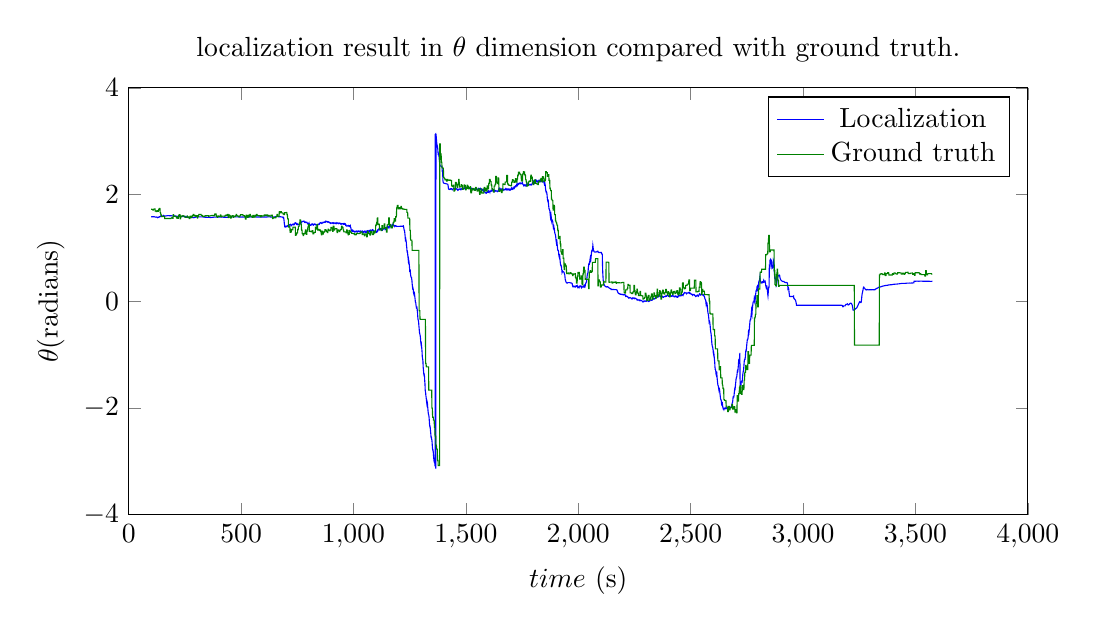
\begin{tikzpicture}

\begin{axis}[
title={localization result in $\theta$ dimension compared with ground truth.},
xlabel={$time$ (s)},
ylabel={$\theta$(radians)},
xmin=0, xmax=4000,
ymin=-4, ymax=4,
axis on top,
width=13cm,
height=7cm,
legend entries={{Localization},{Ground truth}}
]
\addplot [blue]
coordinates {
(100,1.58331552346284)
(101,1.58263161976869)
(102,1.58266988595063)
(103,1.58279410203034)
(104,1.58297530015046)
(105,1.58365169365937)
(106,1.58342877228791)
(107,1.58282700379426)
(108,1.58255091507966)
(109,1.58259371121461)
(110,1.58257618744905)
(111,1.5826554616266)
(112,1.58244827588136)
(113,1.58316317399079)
(114,1.58321777184541)
(115,1.58231404622132)
(116,1.58214274247224)
(117,1.57989087899263)
(118,1.57895091374452)
(119,1.57639160950715)
(120,1.57553878624971)
(121,1.57462886174256)
(122,1.57492867310578)
(123,1.575836571055)
(124,1.57872370083863)
(125,1.57819310029084)
(126,1.57567647297914)
(127,1.57296517689759)
(128,1.56945052941377)
(129,1.56545189221437)
(130,1.56746474106843)
(131,1.57085755665834)
(132,1.57214501698548)
(133,1.57517102559144)
(134,1.57903078396852)
(135,1.58283415635163)
(136,1.58312097390229)
(137,1.57932678063447)
(138,1.57832160790498)
(139,1.58306184609468)
(140,1.58838167985017)
(141,1.59062496026094)
(142,1.59516170819337)
(143,1.59831300576264)
(144,1.59642353852326)
(145,1.59137061436708)
(146,1.59446385701234)
(147,1.5916647036844)
(148,1.59469238122041)
(149,1.59343138535554)
(150,1.5949389060312)
(151,1.5968965609842)
(152,1.59892204602296)
(153,1.60209122498567)
(154,1.60609284241731)
(155,1.60942951043183)
(156,1.60530200799043)
(157,1.60056117375428)
(158,1.5970700105005)
(159,1.59668377240235)
(160,1.59934607346589)
(161,1.59975365002687)
(162,1.59979930718476)
(163,1.59787848790223)
(164,1.59663298924501)
(165,1.596863540011)
(166,1.5983077605539)
(167,1.60007289250428)
(168,1.60012915928895)
(169,1.60095098813111)
(170,1.60230949719483)
(171,1.60158100922639)
(172,1.60340407689149)
(173,1.60421589215333)
(174,1.60415020783479)
(175,1.60453322728211)
(176,1.60359683831269)
(177,1.60363367398316)
(178,1.60367956955964)
(179,1.60265842278535)
(180,1.60253980954225)
(181,1.60225251515443)
(182,1.60228648980195)
(183,1.60208979447419)
(184,1.60207846959169)
(185,1.60170534451539)
(186,1.60153189499909)
(187,1.60144522984559)
(188,1.60140422184999)
(189,1.60055199463899)
(190,1.6003761609369)
(191,1.60134390194947)
(192,1.60135594208772)
(193,1.60022834141786)
(194,1.6002723296457)
(195,1.600290568667)
(196,1.59986582596833)
(197,1.60003784497315)
(198,1.59944024880464)
(199,1.59928003151948)
(200,1.59926977952058)
(201,1.59888723691041)
(202,1.59827664692933)
(203,1.59784189065034)
(204,1.59764853318269)
(205,1.5974669774347)
(206,1.59814086754853)
(207,1.59678200085694)
(208,1.59571877320344)
(209,1.59642568429048)
(210,1.5942634661966)
(211,1.59329739411409)
(212,1.59295109112794)
(213,1.59268441994721)
(214,1.59231284459169)
(215,1.59314182599122)
(216,1.59114280541474)
(217,1.5912380536371)
(218,1.59084847767884)
(219,1.59046045144136)
(220,1.5893624146753)
(221,1.58917597134645)
(222,1.59000399907167)
(223,1.58865609963471)
(224,1.58948388894136)
(225,1.58936169941957)
(226,1.58828130562837)
(227,1.5879317839914)
(228,1.58791378338868)
(229,1.58797195752198)
(230,1.58922985394532)
(231,1.58813610871369)
(232,1.58801785309846)
(233,1.58799520333345)
(234,1.58757940133149)
(235,1.58798268635804)
(236,1.58756020863587)
(237,1.58807292779023)
(238,1.58765509923036)
(239,1.58768442471559)
(240,1.58769014676149)
(241,1.58751252492005)
(242,1.58782151539857)
(243,1.58760586579377)
(244,1.58765724499757)
(245,1.58800640900666)
(246,1.58777621586854)
(247,1.5881086905771)
(248,1.58787778218324)
(249,1.58806565602357)
(250,1.58826962311799)
(251,1.58834973176057)
(252,1.59004941781098)
(253,1.59002784092958)
(254,1.58788803418214)
(255,1.5858657677942)
(256,1.58450284798677)
(257,1.58128574688966)
(258,1.58036819298799)
(259,1.57832828362519)
(260,1.57562950451905)
(261,1.57341054280336)
(262,1.57068279583985)
(263,1.56970086892182)
(264,1.56916085084016)
(265,1.56887534459169)
(266,1.56858876545961)
(267,1.56787041028077)
(268,1.5677742083841)
(269,1.56759336789186)
(270,1.56779101689393)
(271,1.56624868710572)
(272,1.5670976956659)
(273,1.56604436238343)
(274,1.56596675713594)
(275,1.56696036656434)
(276,1.56705287297303)
(277,1.56592503388459)
(278,1.56701639493043)
(279,1.56600550015504)
(280,1.56639424164826)
(281,1.566345961886)
(282,1.56627431710298)
(283,1.56619849999482)
(284,1.5664725621515)
(285,1.56695094903047)
(286,1.56681159337098)
(287,1.56554213364656)
(288,1.56579438050325)
(289,1.5659398158365)
(290,1.56614116032655)
(291,1.56811216671998)
(292,1.5680777152353)
(293,1.5695562680536)
(294,1.57186523278291)
(295,1.57269004185731)
(296,1.57260659535462)
(297,1.57396426995332)
(298,1.57513800461824)
(299,1.57591811020906)
(300,1.5776745398813)
(301,1.57814958890016)
(302,1.57883671124513)
(303,1.57908252080018)
(304,1.57913902600343)
(305,1.57958820660646)
(306,1.57977321942384)
(307,1.57979622681672)
(308,1.57970372040803)
(309,1.57981172402436)
(310,1.57976559002931)
(311,1.5798204263025)
(312,1.57978645165498)
(313,1.58084312279756)
(314,1.57976439793641)
(315,1.57987156708772)
(316,1.57985368569429)
(317,1.5798249562555)
(318,1.57999184926087)
(319,1.58018568356568)
(320,1.58037880261476)
(321,1.5808962901407)
(322,1.58116355736787)
(323,1.58129742940003)
(324,1.58158460457856)
(325,1.58189740975434)
(326,1.58189442952211)
(327,1.58179226716096)
(328,1.5813457091623)
(329,1.58076754410798)
(330,1.58033076127107)
(331,1.57966748078401)
(332,1.57916572888429)
(333,1.57896152337129)
(334,1.57868817647035)
(335,1.57768443425233)
(336,1.57693234284455)
(337,1.57534125645692)
(338,1.57486716111238)
(339,1.57423535187776)
(340,1.57383623917634)
(341,1.57372740109498)
(342,1.57352557976777)
(343,1.57353142102296)
(344,1.57328298886354)
(345,1.57330742676789)
(346,1.57335236867005)
(347,1.57349470456178)
(348,1.57095208962495)
(349,1.5707964022928)
(350,1.57082525094087)
(351,1.57115355332429)
(352,1.57072177727754)
(353,1.57086852391297)
(354,1.57069960434968)
(355,1.57078054745729)
(356,1.57072475750978)
(357,1.57070329983766)
(358,1.57053354580934)
(359,1.5705932696634)
(360,1.57034197648103)
(361,1.57003858883912)
(362,1.56995132763917)
(363,1.56975963910157)
(364,1.5696760733896)
(365,1.56968417962129)
(366,1.56959429581697)
(367,1.56968739827211)
(368,1.57025030453736)
(369,1.57065215905244)
(370,1.57132330735261)
(371,1.57170489628846)
(372,1.57201734383638)
(373,1.57264355023439)
(374,1.57321921189363)
(375,1.57344499428804)
(376,1.57384935219819)
(377,1.5747379382425)
(378,1.57534089882905)
(379,1.57598868210847)
(380,1.57610073884065)
(381,1.57626727421815)
(382,1.57654896576936)
(383,1.57632640202577)
(384,1.57633474667604)
(385,1.57641914685304)
(386,1.57635405858094)
(387,1.57645216782624)
(388,1.57644775708253)
(389,1.57646468480165)
(390,1.57647684414918)
(391,1.5761708339029)
(392,1.57610455353791)
(393,1.57598594029481)
(394,1.5762107690149)
(395,1.57630530198152)
(396,1.57647994359071)
(397,1.57645419438417)
(398,1.57675317128236)
(399,1.57738998730714)
(400,1.57733598549897)
(401,1.57781270344789)
(402,1.57796517212922)
(403,1.57811954815919)
(404,1.57822683651979)
(405,1.57845786412294)
(406,1.57836237748201)
(407,1.57833257515962)
(408,1.57815376122529)
(409,1.57822635968263)
(410,1.57777741749818)
(411,1.57765272458131)
(412,1.57727197011048)
(413,1.57679406006867)
(414,1.57635787327821)
(415,1.5757886489206)
(416,1.57550469239289)
(417,1.57543745835359)
(418,1.57547918160493)
(419,1.57532122929628)
(420,1.57519379456575)
(421,1.57504669030244)
(422,1.57497933705384)
(423,1.57491842110688)
(424,1.57496622403199)
(425,1.57490173180635)
(426,1.57490804989869)
(427,1.57490232785279)
(428,1.57489386399324)
(429,1.57489529450471)
(430,1.57479849656159)
(431,1.5747596343332)
(432,1.57477715809877)
(433,1.57485404809053)
(434,1.57474473317201)
(435,1.57466677029664)
(436,1.57478681405122)
(437,1.57485071023042)
(438,1.57491508324678)
(439,1.57472470601136)
(440,1.57474461396272)
(441,1.57480040391023)
(442,1.57477382023866)
(443,1.57490042050416)
(444,1.57492700417573)
(445,1.57521012623841)
(446,1.57560864289338)
(447,1.57592252095277)
(448,1.5760886987024)
(449,1.57643988926942)
(450,1.5766625722223)
(451,1.57710424264009)
(452,1.57750132878358)
(453,1.57790509064729)
(454,1.5786259492212)
(455,1.57906010945375)
(456,1.57940271695191)
(457,1.57985273201997)
(458,1.58010974724824)
(459,1.58016231854493)
(460,1.58027532895143)
(461,1.58037844498689)
(462,1.58039728005464)
(463,1.58037558396394)
(464,1.58036878903443)
(465,1.58031526406343)
(466,1.58040121396119)
(467,1.58041003544862)
(468,1.58042374451692)
(469,1.58041802247102)
(470,1.58042410214479)
(471,1.58043030102784)
(472,1.58033123810823)
(473,1.58054653008515)
(474,1.58061531384523)
(475,1.58056011994416)
(476,1.58080092270906)
(477,1.58090868790681)
(478,1.58105793793733)
(479,1.58116677601869)
(480,1.58129039605195)
(481,1.58129766781861)
(482,1.58163979847962)
(483,1.58124676545198)
(484,1.58108511765534)
(485,1.58090678055818)
(486,1.58070424397523)
(487,1.58048287232453)
(488,1.58030143578584)
(489,1.58006826241548)
(490,1.57973972161347)
(491,1.57938078244264)
(492,1.57896986802156)
(493,1.57876363595063)
(494,1.57836368878419)
(495,1.57812228997285)
(496,1.57802418072755)
(497,1.57800319989259)
(498,1.57792976697023)
(499,1.57776668866212)
(500,1.57771435578401)
(501,1.57764008839662)
(502,1.57768300374086)
(503,1.57769707043702)
(504,1.57773140271241)
(505,1.577749760943)
(506,1.57778087456758)
(507,1.57776180108125)
(508,1.577785166102)
(509,1.57776311238343)
(510,1.57771149476106)
(511,1.5775934775644)
(512,1.57756772835786)
(513,1.57753291924531)
(514,1.57751324971253)
(515,1.57750657399232)
(516,1.5774052460962)
(517,1.57736960251863)
(518,1.57718768914277)
(519,1.57719162304933)
(520,1.57699635823304)
(521,1.57705894311006)
(522,1.57706001599366)
(523,1.57702413399751)
(524,1.57711973984773)
(525,1.57724395592744)
(526,1.57737115223939)
(527,1.57757571538026)
(528,1.57780495484407)
(529,1.57797935803468)
(530,1.5781388600641)
(531,1.5782962163263)
(532,1.57860258420045)
(533,1.57874039013917)
(534,1.57891407807405)
(535,1.57912066777284)
(536,1.57926300366456)
(537,1.57953253586824)
(538,1.57969322999055)
(539,1.57968059380586)
(540,1.57973817189271)
(541,1.57972088654573)
(542,1.57969787915284)
(543,1.57968905766542)
(544,1.57967165310914)
(545,1.57962134678895)
(546,1.57973996003205)
(547,1.57975247700746)
(548,1.57972791989381)
(549,1.5797497351938)
(550,1.579778226214)
(551,1.57975486119325)
(552,1.57976868947084)
(553,1.57983854611451)
(554,1.57994201977784)
(555,1.58003333409364)
(556,1.58007469971711)
(557,1.58019188244874)
(558,1.58032515843446)
(559,1.58040836651857)
(560,1.58037081559236)
(561,1.58051589329774)
(562,1.58048871357972)
(563,1.5804080088907)
(564,1.58027318318421)
(565,1.58010593255097)
(566,1.57996443112428)
(567,1.57971027691896)
(568,1.57966831524903)
(569,1.57949021657044)
(570,1.57928171952302)
(571,1.5790560563379)
(572,1.57869568665559)
(573,1.57862416108186)
(574,1.57834246953065)
(575,1.57840910752351)
(576,1.57827237446839)
(577,1.57821670373017)
(578,1.57804516156251)
(579,1.57802728016908)
(580,1.57795694668824)
(581,1.57826081116731)
(582,1.57789030869538)
(583,1.57776990731294)
(584,1.57790473301942)
(585,1.5779619534784)
(586,1.57779577572877)
(587,1.57791331608827)
(588,1.57796445687348)
(589,1.57789841492707)
(590,1.57791260083253)
(591,1.57792166073854)
(592,1.57785955269868)
(593,1.57780578930909)
(594,1.57768109639222)
(595,1.57773640950257)
(596,1.57769170601899)
(597,1.57757607300813)
(598,1.57755807240541)
(599,1.57753613789613)
(600,1.57749405701692)
(601,1.5774942954355)
(602,1.57743004162843)
(603,1.57791426976258)
(604,1.57769182522828)
(605,1.57781949837739)
(606,1.57791844208772)
(607,1.57805767853791)
(608,1.57816222508485)
(609,1.5783783515268)
(610,1.57846835454042)
(611,1.57856813271577)
(612,1.57881024678285)
(613,1.57895639737184)
(614,1.57915595372254)
(615,1.57929375966127)
(616,1.57941225369508)
(617,1.57956245739991)
(618,1.57995906670625)
(619,1.58010354836518)
(620,1.58016184170777)
(621,1.58124998410279)
(622,1.57998064358766)
(623,1.57994988759095)
(624,1.57995489438111)
(625,1.58000830014283)
(626,1.57997349103028)
(627,1.58012774785096)
(628,1.58019450505311)
(629,1.58010009129579)
(630,1.57931724389131)
(631,1.57918599446351)
(632,1.57828274567659)
(633,1.5783555825525)
(634,1.57730356057221)
(635,1.57817223866517)
(636,1.57727149327333)
(637,1.57621851761872)
(638,1.57520356972749)
(639,1.57374337513978)
(640,1.57404878933961)
(641,1.57453277905519)
(642,1.5752034505182)
(643,1.57622304757173)
(644,1.57660427887971)
(645,1.57637945015962)
(646,1.57809141476686)
(647,1.57897404034669)
(648,1.58065250714357)
(649,1.57956794102723)
(650,1.58080640633638)
(651,1.58240476449067)
(652,1.58188012440736)
(653,1.58249715169007)
(654,1.58355167706544)
(655,1.58412113984162)
(656,1.58481636841828)
(657,1.58535340626771)
(658,1.58544329007203)
(659,1.58524707158143)
(660,1.58563772042329)
(661,1.58607784112031)
(662,1.58487251599366)
(663,1.58598163922364)
(664,1.58513954480226)
(665,1.58440199692781)
(666,1.58477369149263)
(667,1.58389619191224)
(668,1.58470002015168)
(669,1.58370664914186)
(670,1.5831380208307)
(671,1.58323338826234)
(672,1.58367625077302)
(673,1.58272817929322)
(674,1.58331719239289)
(675,1.58180931408937)
(676,1.58286276658113)
(677,1.58188846905763)
(678,1.58066085179383)
(679,1.58093992074067)
(680,1.58040693600709)
(681,1.57964483101899)
(682,1.57890251477296)
(683,1.57742217381532)
(684,1.57464578946168)
(685,1.57193091710145)
(686,1.56828943093354)
(687,1.56514981587464)
(688,1.55902877648408)
(689,1.56584492524201)
(690,1.55375507672364)
(691,1.51356044610078)
(692,1.46938184102113)
(693,1.43603339989717)
(694,1.40637985070283)
(695,1.41156104405458)
(696,1.40219178994233)
(697,1.38938692410524)
(698,1.389313133555)
(699,1.39171639283235)
(700,1.40081706841523)
(701,1.39757242997224)
(702,1.40059128602082)
(703,1.40055039723451)
(704,1.40890565712983)
(705,1.4086448272043)
(706,1.40760508378083)
(707,1.41698518593843)
(708,1.41761949856813)
(709,1.41282800038392)
(710,1.40418628056581)
(711,1.40106764634187)
(712,1.40639916260774)
(713,1.41687432129914)
(714,1.42426398594911)
(715,1.42864433129365)
(716,1.4362919648462)
(717,1.43661204178865)
(718,1.4380625804239)
(719,1.44078973134095)
(720,1.44205835660035)
(721,1.43315020402009)
(722,1.41488543351228)
(723,1.41606334050233)
(724,1.41450050671632)
(725,1.42296496232087)
(726,1.42954650719697)
(727,1.43184963067109)
(728,1.43649438221986)
(729,1.43984654744203)
(730,1.43889454205567)
(731,1.44788256485993)
(732,1.44833556016023)
(733,1.44417241414125)
(734,1.43619421322877)
(735,1.43034985859925)
(736,1.43206134636933)
(737,1.44062069256837)
(738,1.45099213917787)
(739,1.45364740689332)
(740,1.47004834015901)
(741,1.47142294247682)
(742,1.4659984429651)
(743,1.46705308754975)
(744,1.46574202378327)
(745,1.46329036553437)
(746,1.44558099110658)
(747,1.4411155303293)
(748,1.44607320626313)
(749,1.44604113896424)
(750,1.43971279461915)
(751,1.4478361924463)
(752,1.4419004042917)
(753,1.43763676484162)
(754,1.43600371678407)
(755,1.43558064301545)
(756,1.43680563767488)
(757,1.43542781670625)
(758,1.43790152867372)
(759,1.43624249299104)
(760,1.43254235585267)
(761,1.44050803978974)
(762,1.45161310036714)
(763,1.46112755139405)
(764,1.46414974530274)
(765,1.48459199269349)
(766,1.4810290654474)
(767,1.47982838948304)
(768,1.47944286664064)
(769,1.47307840188081)
(770,1.48410645325715)
(771,1.49603977997834)
(772,1.49463466008241)
(773,1.49647537072236)
(774,1.49687698681886)
(775,1.4957698901468)
(776,1.49870863755281)
(777,1.50107577641542)
(778,1.50179222424562)
(779,1.49817899067933)
(780,1.5012196620279)
(781,1.49147811730439)
(782,1.48341313202912)
(783,1.47626999218995)
(784,1.4750202019983)
(785,1.47687855561311)
(786,1.47988072236116)
(787,1.48363521893556)
(788,1.47775009472901)
(789,1.47965648968751)
(790,1.48262003262574)
(791,1.48162725766236)
(792,1.47931304772431)
(793,1.48032537301118)
(794,1.46696534951264)
(795,1.45783379872377)
(796,1.45004621346528)
(797,1.45299342473085)
(798,1.45715406735475)
(799,1.45925286610658)
(800,1.45470717747743)
(801,1.45446065266664)
(802,1.46336832840974)
(803,1.43434432347352)
(804,1.43212631543214)
(805,1.43000164826448)
(806,1.43953755696351)
(807,1.43463972409303)
(808,1.42250278790528)
(809,1.42048815091188)
(810,1.42050185998017)
(811,1.42938557465608)
(812,1.43061235745484)
(813,1.43261340458924)
(814,1.44347325165803)
(815,1.44811931450898)
(816,1.44221309025819)
(817,1.44333806832368)
(818,1.44816854794557)
(819,1.44703605969483)
(820,1.43511703808839)
(821,1.42380407651002)
(822,1.42572501500184)
(823,1.43056503136689)
(824,1.43873146374757)
(825,1.44093325932557)
(826,1.44652024109895)
(827,1.44887069066102)
(828,1.44697872002656)
(829,1.44234517415101)
(830,1.43892303307588)
(831,1.44137075741822)
(832,1.43711021740968)
(833,1.42723134358461)
(834,1.42687347729737)
(835,1.42637327511842)
(836,1.43151942093904)
(837,1.43058517773683)
(838,1.42789736588533)
(839,1.43476358254487)
(840,1.43695274193818)
(841,1.43509248097474)
(842,1.43439570267732)
(843,1.43976393540437)
(844,1.44549265702302)
(845,1.44610944588716)
(846,1.43779459794099)
(847,1.43867126305635)
(848,1.44423774083192)
(849,1.45575776894624)
(850,1.46127549012239)
(851,1.46682813962037)
(852,1.47304347355897)
(853,1.47074154217774)
(854,1.46685138543183)
(855,1.46851542790467)
(856,1.47312393982942)
(857,1.46648875077302)
(858,1.45701721509034)
(859,1.45577946503694)
(860,1.45906916459138)
(861,1.46554520924623)
(862,1.46947649319703)
(863,1.47197488148744)
(864,1.47991660435731)
(865,1.47790220578248)
(866,1.47400430043275)
(867,1.4762146790796)
(868,1.48029497464234)
(869,1.48312238057191)
(870,1.48061052163179)
(871,1.4795904477411)
(872,1.4800205548578)
(873,1.48898902733857)
(874,1.49104705651338)
(875,1.48608270485932)
(876,1.49811020691926)
(877,1.50193169911439)
(878,1.49942210515077)
(879,1.49574008782441)
(880,1.49711004097993)
(881,1.49730804760987)
(882,1.49282911618287)
(883,1.48484185536439)
(884,1.48517969449098)
(885,1.48833313782746)
(886,1.48069802125032)
(887,1.47948637803132)
(888,1.48810592492158)
(889,1.48943963845307)
(890,1.48767116864259)
(891,1.48268428643281)
(892,1.48012271721894)
(893,1.47939744790132)
(894,1.47316006024415)
(895,1.4670731147104)
(896,1.46800878842408)
(897,1.46981492837007)
(898,1.4615674336725)
(899,1.45602622826631)
(900,1.45799520810182)
(901,1.46400955517823)
(902,1.46828511555726)
(903,1.46748104889924)
(904,1.46643296082551)
(905,1.46570041974122)
(906,1.46898248990113)
(907,1.46155873139436)
(908,1.45899966557557)
(909,1.46119931538636)
(910,1.46713307698304)
(911,1.4589171727472)
(912,1.45565429528291)
(913,1.46312025387818)
(914,1.46794453461701)
(915,1.4684375842386)
(916,1.46491757233674)
(917,1.46178785164888)
(918,1.45906415780122)
(919,1.46369484265382)
(920,1.45461181004579)
(921,1.4551045020395)
(922,1.45935574372346)
(923,1.46187249024446)
(924,1.45604863961274)
(925,1.46102813084657)
(926,1.47248855431611)
(927,1.47043231328065)
(928,1.46780887444551)
(929,1.46506717999513)
(930,1.45943394501741)
(931,1.45563164551789)
(932,1.45390692551667)
(933,1.45273998578126)
(934,1.45716014702851)
(935,1.46314028103883)
(936,1.4561107476526)
(937,1.46012106736238)
(938,1.46513083775575)
(939,1.46563807328279)
(940,1.4625188430124)
(941,1.46107402642305)
(942,1.45867338975007)
(943,1.45668533642823)
(944,1.44313505490357)
(945,1.44285372098024)
(946,1.44510916073854)
(947,1.45356586773927)
(948,1.44956782658631)
(949,1.44718888600404)
(950,1.4511548598581)
(951,1.45340767701203)
(952,1.45206394990022)
(953,1.45123496850068)
(954,1.45559933980043)
(955,1.45038905938203)
(956,1.44056180317933)
(957,1.44008389313752)
(958,1.44233551819856)
(959,1.45063284237916)
(960,1.44275930722291)
(961,1.44228020508821)
(962,1.44829920132691)
(963,1.45183614094789)
(964,1.44918433030183)
(965,1.42254391511018)
(966,1.42188099225099)
(967,1.42384758790071)
(968,1.40855363209779)
(969,1.40710666974122)
(970,1.40730753739411)
(971,1.41177478631074)
(972,1.41122070153291)
(973,1.40997865994508)
(974,1.415964396792)
(975,1.4188028891855)
(976,1.41600218613679)
(977,1.41424945195253)
(978,1.41865900357301)
(979,1.41331783135469)
(980,1.40350213845307)
(981,1.40111008484895)
(982,1.4037391265207)
(983,1.41020170052583)
(984,1.40681007702882)
(985,1.40804770787294)
(986,1.4152981360727)
(987,1.38203183014924)
(988,1.37965384324128)
(989,1.35653630097444)
(990,1.34079435666139)
(991,1.33168831666047)
(992,1.32530275185639)
(993,1.31030383904512)
(994,1.31448808510835)
(995,1.32340708573396)
(996,1.31668368180329)
(997,1.32871225674684)
(998,1.32374456723268)
(999,1.3153237422281)
(1000,1.31149545510346)
(1001,1.3137185891443)
(1002,1.31540742714936)
(1003,1.30311039288575)
(1004,1.29819336731965)
(1005,1.29815307457978)
(1006,1.30321493943269)
(1007,1.30427316029603)
(1008,1.30000880559022)
(1009,1.30270973046357)
(1010,1.31367269356782)
(1011,1.3137243111902)
(1012,1.30989614327485)
(1013,1.31163528760011)
(1014,1.31467595894868)
(1015,1.311148198443)
(1016,1.30134740670259)
(1017,1.30111673672731)
(1018,1.29773715336854)
(1019,1.30855253537232)
(1020,1.30387702782685)
(1021,1.30584243138368)
(1022,1.31390956242616)
(1023,1.30818560917909)
(1024,1.30507484276826)
(1025,1.30553892453248)
(1026,1.31173244317109)
(1027,1.30756953557069)
(1028,1.29707780678804)
(1029,1.29466441472108)
(1030,1.29484680493409)
(1031,1.30447367032106)
(1032,1.28982439835603)
(1033,1.29043331940705)
(1034,1.30181279976899)
(1035,1.30838898022706)
(1036,1.3051405270868)
(1037,1.30732777913148)
(1038,1.30559244950349)
(1039,1.31286421616609)
(1040,1.30426982243592)
(1041,1.2921440919214)
(1042,1.29831555684144)
(1043,1.3019519170099)
(1044,1.29925635655458)
(1045,1.28846696217591)
(1046,1.29293707211549)
(1047,1.30556407769258)
(1048,1.30404833157594)
(1049,1.30469146569306)
(1050,1.30975976784761)
(1051,1.31532851059968)
(1052,1.31054154236848)
(1053,1.29254487355287)
(1054,1.29500511487062)
(1055,1.29511490662629)
(1056,1.30370417435701)
(1057,1.29163137276704)
(1058,1.29184761841828)
(1059,1.30474570591981)
(1060,1.30812147458131)
(1061,1.30529764493043)
(1062,1.30877426465089)
(1063,1.32203319867189)
(1064,1.32073870499665)
(1065,1.30646565754945)
(1066,1.2995595057779)
(1067,1.30079832871492)
(1068,1.29307058651979)
(1069,1.30778315861756)
(1070,1.29690531094606)
(1071,1.30410996277864)
(1072,1.31862107117707)
(1073,1.31309572060639)
(1074,1.3157903273874)
(1075,1.31544485886628)
(1076,1.33267954190309)
(1077,1.33047452767427)
(1078,1.31625262101228)
(1079,1.31029883225495)
(1080,1.30682912667329)
(1081,1.31818714936311)
(1082,1.32616964181001)
(1083,1.32254448731477)
(1084,1.33913818200166)
(1085,1.34186819394166)
(1086,1.33684650261933)
(1087,1.33658471901948)
(1088,1.32974448998506)
(1089,1.32799485524232)
(1090,1.31430509884889)
(1091,1.31508472760255)
(1092,1.30494788487489)
(1093,1.31153515179689)
(1094,1.30833044846589)
(1095,1.3080314715677)
(1096,1.31117585499818)
(1097,1.31164518197114)
(1098,1.30021420319612)
(1099,1.30056384404237)
(1100,1.29705003102357)
(1101,1.31411722500856)
(1102,1.31254211266572)
(1103,1.29364755948121)
(1104,1.29651656945283)
(1105,1.29772356350953)
(1106,1.30631235440309)
(1107,1.32287302811677)
(1108,1.31949892838533)
(1109,1.33872452576692)
(1110,1.33639362652833)
(1111,1.33975389798219)
(1112,1.33936765988404)
(1113,1.35620919068391)
(1114,1.36140898068482)
(1115,1.35219446023042)
(1116,1.33962777455384)
(1117,1.33278694947297)
(1118,1.33332374890382)
(1119,1.34746840794618)
(1120,1.35444012482698)
(1121,1.36254957516725)
(1122,1.36404970486695)
(1123,1.36136976082856)
(1124,1.36184802849824)
(1125,1.35747948487336)
(1126,1.36126855214173)
(1127,1.3604475577646)
(1128,1.33091297944123)
(1129,1.33089092572267)
(1130,1.33980456193025)
(1131,1.34501245816285)
(1132,1.35719981988008)
(1133,1.35913756688172)
(1134,1.35768130620057)
(1135,1.3588776906305)
(1136,1.36085453827912)
(1137,1.36804822285707)
(1138,1.36469474633271)
(1139,1.36044851143891)
(1140,1.36009767849977)
(1141,1.3422556241327)
(1142,1.34651282628114)
(1143,1.34782353241975)
(1144,1.35420742829377)
(1145,1.36802712281282)
(1146,1.37477222283418)
(1147,1.38294938405091)
(1148,1.38013830979402)
(1149,1.38261106808717)
(1150,1.38947561581666)
(1151,1.40077021916444)
(1152,1.3876692374521)
(1153,1.37670198281343)
(1154,1.37974515755708)
(1155,1.38146117528016)
(1156,1.38727179368074)
(1157,1.39473834832246)
(1158,1.38094321091706)
(1159,1.39786628087098)
(1160,1.40551462967927)
(1161,1.39889064629609)
(1162,1.4051035960489)
(1163,1.41169265111024)
(1164,1.421166690188)
(1165,1.41300144990022)
(1166,1.40283134778077)
(1167,1.40005186398561)
(1168,1.39964261849458)
(1169,1.40875068505342)
(1170,1.41542974312837)
(1171,1.40084174473817)
(1172,1.42214825947816)
(1173,1.43343332608277)
(1174,1.42601815064485)
(1175,1.42796114285524)
(1176,1.43659249146516)
(1177,1.43299547036225)
(1178,1.43164614041383)
(1179,1.41544786294038)
(1180,1.41874340375001)
(1181,1.42004826863343)
(1182,1.41300764878327)
(1183,1.40955093701417)
(1184,1.40086558659608)
(1185,1.40682295163209)
(1186,1.41361132462556)
(1187,1.40967026551301)
(1188,1.41136840184266)
(1189,1.41371265252168)
(1190,1.40769615967805)
(1191,1.40609887440736)
(1192,1.40204993088777)
(1193,1.40053275425965)
(1194,1.40120700200135)
(1195,1.40207901795442)
(1196,1.40296665032441)
(1197,1.40246787865693)
(1198,1.40312949021394)
(1199,1.40261760552461)
(1200,1.40330055554444)
(1201,1.40195122559602)
(1202,1.40303161938722)
(1203,1.40385034878785)
(1204,1.40385690529878)
(1205,1.40276852448518)
(1206,1.40391579468782)
(1207,1.40437045891816)
(1208,1.40438726742799)
(1209,1.40448764164979)
(1210,1.40458980401094)
(1211,1.40443435509736)
(1212,1.40556326706941)
(1213,1.4042833169275)
(1214,1.40542653401429)
(1215,1.40526417096192)
(1216,1.40516987641389)
(1217,1.40513387520845)
(1218,1.40509000618989)
(1219,1.40539172490174)
(1220,1.40670517285401)
(1221,1.40998795826966)
(1222,1.41203752358491)
(1223,1.39199033577973)
(1224,1.36748257477815)
(1225,1.34626725514466)
(1226,1.32598045666749)
(1227,1.32674327691133)
(1228,1.29610601265962)
(1229,1.24774757226045)
(1230,1.21188643773133)
(1231,1.13978067238862)
(1232,1.14366486867005)
(1233,1.1574001630121)
(1234,1.13395944436128)
(1235,1.10187617142732)
(1236,1.04147473176057)
(1237,1.0067390521341)
(1238,0.950888784723826)
(1239,0.922097595530101)
(1240,0.926589163141795)
(1241,0.888864429789134)
(1242,0.842729719477244)
(1243,0.813042076426097)
(1244,0.765646608667918)
(1245,0.787638099985667)
(1246,0.761133344965526)
(1247,0.733481319742747)
(1248,0.692033441858836)
(1249,0.649783523874827)
(1250,0.583743723230906)
(1251,0.593389662104197)
(1252,0.591675909357615)
(1253,0.556036146479197)
(1254,0.495207937555858)
(1255,0.469151171045848)
(1256,0.452831896143504)
(1257,0.446043165522166)
(1258,0.445200594263621)
(1259,0.419157179194041)
(1260,0.38951817353303)
(1261,0.326607855158397)
(1262,0.290011080103465)
(1263,0.250955494242259)
(1264,0.259377630549022)
(1265,0.24228278000886)
(1266,0.215898426371165)
(1267,0.161659153299876)
(1268,0.144351871805735)
(1269,0.171490820246287)
(1270,0.171878488855906)
(1271,0.155569942789622)
(1272,0.117523105936595)
(1273,0.0784050544076642)
(1274,0.0449606498056134)
(1275,-0.0023988803201398)
(1276,-0.022632511454173)
(1277,-0.0267788489633283)
(1278,-0.0685478766732892)
(1279,-0.0964254458718976)
(1280,-0.122933061914988)
(1281,-0.119040401773997)
(1282,-0.114030750589915)
(1283,-0.132427843409129)
(1284,-0.184396179514476)
(1285,-0.222729595499583)
(1286,-0.289716871576854)
(1287,-0.339229257898875)
(1288,-0.35395875771577)
(1289,-0.362687261896678)
(1290,-0.401672991114207)
(1291,-0.462942274408885)
(1292,-0.504583986597606)
(1293,-0.55730381806428)
(1294,-0.596202286081859)
(1295,-0.611105354624339)
(1296,-0.633350046473094)
(1297,-0.652686746912547)
(1298,-0.692961605387278)
(1299,-0.752374323206492)
(1300,-0.792766722040721)
(1301,-0.818972023325511)
(1302,-0.803461702662059)
(1303,-0.84537139733369)
(1304,-0.889654548960277)
(1305,-0.945587547617503)
(1306,-1.03348127205903)
(1307,-1.06630101998384)
(1308,-1.08828941186006)
(1309,-1.12654105027253)
(1310,-1.23583105404908)
(1311,-1.27667525609071)
(1312,-1.32400468190248)
(1313,-1.37694862683351)
(1314,-1.39207318623597)
(1315,-1.38208690484101)
(1316,-1.40886917908723)
(1317,-1.49736896355683)
(1318,-1.54300013382966)
(1319,-1.65922740300233)
(1320,-1.70085838635499)
(1321,-1.71054485638673)
(1322,-1.77331343491609)
(1323,-1.79163387616212)
(1324,-1.83267966111238)
(1325,-1.87471166451509)
(1326,-1.90778187115724)
(1327,-1.87347045739228)
(1328,-1.88864043553407)
(1329,-1.91650739510591)
(1330,-1.97802463372285)
(1331,-2.01827207406098)
(1332,-2.07235780556733)
(1333,-2.10660472710664)
(1334,-2.12765875657136)
(1335,-2.13776532013948)
(1336,-2.16930917103822)
(1337,-2.21960374911363)
(1338,-2.29011604388291)
(1339,-2.33761719067628)
(1340,-2.35305139620835)
(1341,-2.34995034535462)
(1342,-2.40291217167909)
(1343,-2.4457974751764)
(1344,-2.48725089629228)
(1345,-2.54490480025346)
(1346,-2.56083366473252)
(1347,-2.55749628146226)
(1348,-2.58677026827867)
(1349,-2.61191699107225)
(1350,-2.66109368403489)
(1351,-2.72997778852517)
(1352,-2.77325386007363)
(1353,-2.79446453054483)
(1354,-2.79235285718972)
(1355,-2.83029455144937)
(1356,-2.89421862562234)
(1357,-2.93815082510049)
(1358,-2.98841208417947)
(1359,-3.01211685140664)
(1360,-3.02236741979653)
(1361,-3.00995630224282)
(1362,-3.03983634908731)
(1363,-3.09654396970803)
(1364,3.12701183104003)
(1365,3.13218646788085)
(1366,-3.13978410617495)
(1367,3.13741117262328)
(1368,3.0871930663758)
(1369,3.04050260235602)
(1370,2.98533445795114)
(1371,2.94709509809548)
(1372,2.92028111417825)
(1373,2.91397005518014)
(1374,2.88219696481759)
(1375,2.85589903791482)
(1376,2.79275804956491)
(1377,2.74772757490213)
(1378,2.74621826608712)
(1379,2.75428837736184)
(1380,2.72745102842385)
(1381,2.69551819761331)
(1382,2.64518803556497)
(1383,2.60348192055757)
(1384,2.55725208123262)
(1385,2.53690257866914)
(1386,2.53670326073701)
(1387,2.53496423562104)
(1388,2.53559413750703)
(1389,2.53323283989961)
(1390,2.53102365334565)
(1391,2.53023734887178)
(1392,2.52822748024995)
(1393,2.52850881417329)
(1394,2.51192215283448)
(1395,2.43852552969987)
(1396,2.43748411734635)
(1397,2.38463148673112)
(1398,2.25835290749604)
(1399,2.23186007340486)
(1400,2.21963724692399)
(1401,2.21511718829209)
(1402,2.21482500632341)
(1403,2.21200910409028)
(1404,2.20989844401414)
(1405,2.20889470179612)
(1406,2.20913419325883)
(1407,2.20756617386872)
(1408,2.20638629992539)
(1409,2.20451519091661)
(1410,2.20518341858918)
(1411,2.20416251023347)
(1412,2.202152582007)
(1413,2.20083645184571)
(1414,2.19968530734117)
(1415,2.19946387608583)
(1416,2.19749495585496)
(1417,2.19597444136674)
(1418,2.19349500735337)
(1419,2.19420090516145)
(1420,2.18582502205903)
(1421,2.16838905413682)
(1422,2.12654653389985)
(1423,2.10171428521211)
(1424,2.1013173182779)
(1425,2.10117569764192)
(1426,2.09857967694337)
(1427,2.0952195246988)
(1428,2.09881964524324)
(1429,2.1024011691385)
(1430,2.10526624520356)
(1431,2.10086587269837)
(1432,2.09983578522737)
(1433,2.10706427891786)
(1434,2.10773328145082)
(1435,2.10252800782258)
(1436,2.10112622578675)
(1437,2.10432961781556)
(1438,2.09659174283082)
(1439,2.08917930920655)
(1440,2.08676126797731)
(1441,2.08877816994721)
(1442,2.1001228411966)
(1443,2.10351661046083)
(1444,2.1057837327295)
(1445,2.11687544186647)
(1446,2.11572101910646)
(1447,2.11181464989717)
(1448,2.11168602307374)
(1449,2.11101010640199)
(1450,2.10400036175782)
(1451,2.09609285195405)
(1452,2.09597113926942)
(1453,2.09588852723176)
(1454,2.09749332268769)
(1455,2.1046201308542)
(1456,2.1055453141504)
(1457,2.1093226989084)
(1458,2.10854497750337)
(1459,2.10401395161683)
(1460,2.09946933587129)
(1461,2.09802010853822)
(1462,2.10031643708284)
(1463,2.09375599225099)
(1464,2.08032670815522)
(1465,2.08272126515443)
(1466,2.08236172993714)
(1467,2.08449283440644)
(1468,2.09583965142305)
(1469,2.09722522099549)
(1470,2.10091749032075)
(1471,2.1053753217035)
(1472,2.10382667382295)
(1473,2.10151866276795)
(1474,2.10462776024873)
(1475,2.10601583321626)
(1476,2.09963181813294)
(1477,2.089823396998)
(1478,2.0883905013376)
(1479,2.09194103081758)
(1480,2.09786382515962)
(1481,2.10547891457612)
(1482,2.10762325127656)
(1483,2.11546054680879)
(1484,2.11548391182954)
(1485,2.11372724373872)
(1486,2.11290982564027)
(1487,2.11846557457978)
(1488,2.11444726784761)
(1489,2.10323205788667)
(1490,2.10149350960786)
(1491,2.10243740876252)
(1492,2.10677269299562)
(1493,2.1117583831125)
(1494,2.11954620678956)
(1495,2.12090173562104)
(1496,2.12863949139649)
(1497,2.12835458119447)
(1498,2.12479391892488)
(1499,2.12637463410432)
(1500,2.129209907847)
(1501,2.12555280526216)
(1502,2.12244776089723)
(1503,2.12217012246186)
(1504,2.12337222893769)
(1505,2.13091018994386)
(1506,2.12547615368898)
(1507,2.1257473548227)
(1508,2.13289264042909)
(1509,2.13229862053926)
(1510,2.13026765187318)
(1511,2.12943557103211)
(1512,2.13367989857728)
(1513,2.13018265564973)
(1514,2.11438051064546)
(1515,2.11273244221742)
(1516,2.11454227765138)
(1517,2.11674002011354)
(1518,2.1262243111902)
(1519,2.12548425992066)
(1520,2.11756363709504)
(1521,2.12088957627351)
(1522,2.11808040936524)
(1523,2.11487665970857)
(1524,2.11845758755738)
(1525,2.12035551865632)
(1526,2.11403599579866)
(1527,2.1029875596338)
(1528,2.10125771363313)
(1529,2.10321036179597)
(1530,2.10739937623078)
(1531,2.10112992127473)
(1532,2.09843293030793)
(1533,2.1008712371164)
(1534,2.10546902020509)
(1535,2.10539046128327)
(1536,2.09938660462434)
(1537,2.10097065766389)
(1538,2.10278931458528)
(1539,2.08769729931886)
(1540,2.08557263215119)
(1541,2.08638420899446)
(1542,2.08952430089051)
(1543,2.09324088891084)
(1544,2.09652248223359)
(1545,2.09517303307588)
(1546,2.09990135033662)
(1547,2.10141912301118)
(1548,2.09926846821839)
(1549,2.0969707091623)
(1550,2.10161653359468)
(1551,2.09892514546449)
(1552,2.08782640297944)
(1553,2.08469692071015)
(1554,2.08431783516938)
(1555,2.08913865883882)
(1556,2.10402015049989)
(1557,2.11717763741548)
(1558,2.11538425286347)
(1559,2.10801843007142)
(1560,2.10616353352601)
(1561,2.09244659741456)
(1562,2.09264877636964)
(1563,2.10913589795167)
(1564,2.11378601391847)
(1565,2.09853247006471)
(1566,2.08845070202882)
(1567,2.08584800561006)
(1568,2.08295467694337)
(1569,2.08746305306489)
(1570,2.10079625447328)
(1571,2.09824469883973)
(1572,2.07773164113099)
(1573,2.07583907445008)
(1574,2.07629493077333)
(1575,2.08223727543885)
(1576,2.09763100941712)
(1577,2.09891370137269)
(1578,2.07541731198365)
(1579,2.06635955174501)
(1580,2.05303672154481)
(1581,2.06461563904817)
(1582,2.05532565911347)
(1583,2.04859116871888)
(1584,2.04779032071168)
(1585,2.04771784146363)
(1586,2.039614828425)
(1587,2.03480032284791)
(1588,2.03478661377961)
(1589,2.02848425705964)
(1590,2.02254906495149)
(1591,2.02450731595094)
(1592,2.02605501015718)
(1593,2.03017988999421)
(1594,2.03856912453706)
(1595,2.04303792317445)
(1596,2.05318406422669)
(1597,2.05280998547608)
(1598,2.04762330849702)
(1599,2.05507961113984)
(1600,2.07058635552461)
(1601,2.06596639950807)
(1602,2.04655829270417)
(1603,2.05004278023774)
(1604,2.05334308941896)
(1605,2.05593589146669)
(1606,2.05598738987977)
(1607,2.04407265980775)
(1608,2.06521001656587)
(1609,2.0636045058542)
(1610,2.06234887440736)
(1611,2.06243184407289)
(1612,2.07240680058534)
(1613,2.06202367146546)
(1614,2.06327012379701)
(1615,2.0649803002649)
(1616,2.07008686860139)
(1617,2.07935109932954)
(1618,2.07335022290284)
(1619,2.07003477414186)
(1620,2.07408455212648)
(1621,2.08034447033937)
(1622,2.07935551007325)
(1623,2.08017137845094)
(1624,2.07602623303468)
(1625,2.08248117764527)
(1626,2.06515100796754)
(1627,2.05662563641603)
(1628,2.06356170971925)
(1629,2.06940010388429)
(1630,2.06631162961061)
(1631,2.07382515271241)
(1632,2.0760157426172)
(1633,2.07177046139772)
(1634,2.06535366375978)
(1635,2.06471613247926)
(1636,2.06490352948243)
(1637,2.06847503979737)
(1638,2.06777122815187)
(1639,2.065218718844)
(1640,2.05410269101197)
(1641,2.05570581753785)
(1642,2.05558279355104)
(1643,2.05932215054566)
(1644,2.06544855435426)
(1645,2.07770279248292)
(1646,2.09958854516084)
(1647,2.10572698910768)
(1648,2.09890344937379)
(1649,2.09896114666993)
(1650,2.10993889172608)
(1651,2.11772027810151)
(1652,2.10883930523927)
(1653,2.08667543728883)
(1654,2.08874443371827)
(1655,2.09234741528565)
(1656,2.09698513348634)
(1657,2.07896450360353)
(1658,2.07827404339845)
(1659,2.09436419804628)
(1660,2.09885981877381)
(1661,2.09385541279847)
(1662,2.09674433072145)
(1663,2.10001495678956)
(1664,2.10270455678041)
(1665,2.08785394032533)
(1666,2.07911685307557)
(1667,2.08550122578675)
(1668,2.08980182011659)
(1669,2.09288779099519)
(1670,2.08783653576905)
(1671,2.08639601071412)
(1672,2.09401992161805)
(1673,2.09647992451722)
(1674,2.09381488164003)
(1675,2.0942339022928)
(1676,2.10398426850373)
(1677,2.10919359524781)
(1678,2.09238472779328)
(1679,2.08774176438386)
(1680,2.08877650101716)
(1681,2.09084978898103)
(1682,2.09894648392732)
(1683,2.08528843720491)
(1684,2.0853866656595)
(1685,2.10298100312287)
(1686,2.1016744693094)
(1687,2.09636345704133)
(1688,2.09571543534333)
(1689,2.10116425355012)
(1690,2.10369005997712)
(1691,2.0906013568216)
(1692,2.08210078080232)
(1693,2.08158436615998)
(1694,2.08741608460481)
(1695,2.09448567231233)
(1696,2.08155432541902)
(1697,2.08109942277009)
(1698,2.09479275544221)
(1699,2.0948738177591)
(1700,2.0945362170511)
(1701,2.10017433960969)
(1702,2.1176976283365)
(1703,2.12300148804719)
(1704,2.10821190674836)
(1705,2.09474078019197)
(1706,2.09486094315583)
(1707,2.09668770630891)
(1708,2.10639611084992)
(1709,2.11767330964143)
(1710,2.12401858170564)
(1711,2.11046317418153)
(1712,2.11063865025575)
(1713,2.10487893422181)
(1714,2.10527137120301)
(1715,2.11239484150941)
(1716,2.14171603520448)
(1717,2.13991907437379)
(1718,2.14105418522889)
(1719,2.15452459652955)
(1720,2.15888425906236)
(1721,2.14340511162812)
(1722,2.14218059380586)
(1723,2.16327682335908)
(1724,2.16677013238008)
(1725,2.16414514382417)
(1726,2.18280014594133)
(1727,2.17724260886247)
(1728,2.1982091983133)
(1729,2.179991157847)
(1730,2.17166319687898)
(1731,2.1818330009752)
(1732,2.18672892649705)
(1733,2.19393256505067)
(1734,2.19372490246827)
(1735,2.20650205214555)
(1736,2.20988366206224)
(1737,2.2037257870012)
(1738,2.20178076823289)
(1739,2.20989749033982)
(1740,2.20275637705857)
(1741,2.20111951430375)
(1742,2.20347759326036)
(1743,2.20710244973237)
(1744,2.2140795310312)
(1745,2.20104834635789)
(1746,2.20017764170701)
(1747,2.2106660922342)
(1748,2.21233883698518)
(1749,2.21180728276307)
(1750,2.21158161957795)
(1751,2.20726195176179)
(1752,2.21646043856675)
(1753,2.19677248795564)
(1754,2.19138321478898)
(1755,2.19088432391221)
(1756,2.18098792632157)
(1757,2.16628477175767)
(1758,2.16198560793931)
(1759,2.1751978119188)
(1760,2.17746678193147)
(1761,2.17522755463655)
(1762,2.18147227366502)
(1763,2.18540021975572)
(1764,2.17865821917588)
(1765,2.17317566474015)
(1766,2.1650774200731)
(1767,2.17057982285554)
(1768,2.17489257653291)
(1769,2.16714760859544)
(1770,2.17983231146867)
(1771,2.19877770741517)
(1772,2.19309905369813)
(1773,2.1909203847223)
(1774,2.19281903107698)
(1775,2.19712791045243)
(1776,2.19232312043244)
(1777,2.1745817383104)
(1778,2.17489978869493)
(1779,2.17922088702256)
(1780,2.18515607913072)
(1781,2.18881532748277)
(1782,2.1891047676378)
(1783,2.1872063597017)
(1784,2.18486431439454)
(1785,2.18056449492509)
(1786,2.18570837576921)
(1787,2.18910441000993)
(1788,2.19100937445695)
(1789,2.18933996756608)
(1790,2.18107757170732)
(1791,2.17811545928056)
(1792,2.17936715682084)
(1793,2.18261262972886)
(1794,2.19080326159532)
(1795,2.20718786318833)
(1796,2.21965143282945)
(1797,2.22509929736192)
(1798,2.21689579089219)
(1799,2.21700641711289)
(1800,2.2227419932657)
(1801,2.2407535632425)
(1802,2.22764054139192)
(1803,2.20870056946809)
(1804,2.20762244065339)
(1805,2.20959451993043)
(1806,2.21908799012239)
(1807,2.23336878617341)
(1808,2.23764220078523)
(1809,2.25450840790803)
(1810,2.2651790698343)
(1811,2.2542885859781)
(1812,2.25690260727937)
(1813,2.25983801682527)
(1814,2.26357212861116)
(1815,2.24041643937165)
(1816,2.23775330384309)
(1817,2.23928573926026)
(1818,2.24271622498567)
(1819,2.24652424653108)
(1820,2.23577287991578)
(1821,2.2381548007303)
(1822,2.25220146973664)
(1823,2.24814358552034)
(1824,2.24656859238679)
(1825,2.24833765824372)
(1826,2.2659548838907)
(1827,2.26162174542482)
(1828,2.2388438304239)
(1829,2.23686638672883)
(1830,2.23633757432038)
(1831,2.24297502835328)
(1832,2.25448063214357)
(1833,2.24540081818635)
(1834,2.24696055253083)
(1835,2.26611605485017)
(1836,2.26073101361329)
(1837,2.25826016266877)
(1838,2.25481644471223)
(1839,2.2511786540323)
(1840,2.24702635605867)
(1841,2.2367366870218)
(1842,2.23777035077149)
(1843,2.24083319504792)
(1844,2.24927368958528)
(1845,2.242491157847)
(1846,2.23682633240754)
(1847,2.23779621918733)
(1848,2.22416630585725)
(1849,2.20077601273591)
(1850,2.18454113801057)
(1851,2.18928948243196)
(1852,2.2007196863466)
(1853,2.17563852866227)
(1854,2.12926140626008)
(1855,2.09463921387727)
(1856,2.06191340287263)
(1857,2.0484016259485)
(1858,2.05571487744386)
(1859,2.04793134530122)
(1860,2.0292046387964)
(1861,2.00440481503541)
(1862,1.94900861580903)
(1863,1.91088929970796)
(1864,1.88985517819459)
(1865,1.90100696881349)
(1866,1.89921072323854)
(1867,1.85868349869783)
(1868,1.80382374127442)
(1869,1.76935282548005)
(1870,1.73110476334626)
(1871,1.72412994702394)
(1872,1.71373251278932)
(1873,1.70627013047273)
(1874,1.676582249003)
(1875,1.62556734879548)
(1876,1.5920366366678)
(1877,1.6313785632425)
(1878,1.64270535309846)
(1879,1.60813370545442)
(1880,1.5683640559488)
(1881,1.51395645936067)
(1882,1.5353286584192)
(1883,1.52812734444673)
(1884,1.52187255223329)
(1885,1.51114800770814)
(1886,1.50352254708345)
(1887,1.47009721596772)
(1888,1.41816917260224)
(1889,1.38734188874299)
(1890,1.40598538716371)
(1891,1.41185847123201)
(1892,1.37969973881776)
(1893,1.36602881749208)
(1894,1.33344724972779)
(1895,1.29672840436036)
(1896,1.27364590962464)
(1897,1.26272884209687)
(1898,1.24678591092164)
(1899,1.23309603531892)
(1900,1.19756880600984)
(1901,1.14559880097444)
(1902,1.11593452294404)
(1903,1.1528150161081)
(1904,1.15338221390779)
(1905,1.11888852913911)
(1906,1.07486716111238)
(1907,1.02462831337983)
(1908,0.986665161448069)
(1909,0.955676706629344)
(1910,0.951709421473094)
(1911,0.95194140275056)
(1912,0.939203174906321)
(1913,0.887602957087108)
(1914,0.850862177210399)
(1915,0.834855707483836)
(1916,0.859836252527781)
(1917,0.864872129755565)
(1918,0.82673707802827)
(1919,0.768493803339549)
(1920,0.727952631311961)
(1921,0.688399942713328)
(1922,0.672459753351756)
(1923,0.66380229790742)
(1924,0.667515905695506)
(1925,0.655808599787303)
(1926,0.612069280939647)
(1927,0.581496866541453)
(1928,0.537285955744334)
(1929,0.547920854883738)
(1930,0.564669283228465)
(1931,0.559175165491649)
(1932,0.553902777033397)
(1933,0.554638536768504)
(1934,0.552476080256053)
(1935,0.55038562615449)
(1936,0.548362882929393)
(1937,0.533024462061473)
(1938,0.520588310556956)
(1939,0.50520912011201)
(1940,0.493588121729442)
(1941,0.450799377756663)
(1942,0.409947069483348)
(1943,0.396316202478953)
(1944,0.381701143580027)
(1945,0.368340881662913)
(1946,0.357092054682322)
(1947,0.347494037943431)
(1948,0.346464069681712)
(1949,0.340582521753856)
(1950,0.337290199595042)
(1951,0.340779693918773)
(1952,0.344568641977855)
(1953,0.345442684488841)
(1954,0.347355278330394)
(1955,0.347449692087718)
(1956,0.347755106287547)
(1957,0.347119243937083)
(1958,0.34776225884492)
(1959,0.347917707758494)
(1960,0.347715767221995)
(1961,0.347366722422191)
(1962,0.347882183390208)
(1963,0.346405895548411)
(1964,0.345139416056224)
(1965,0.342677505808421)
(1966,0.342057617502757)
(1967,0.342247398691722)
(1968,0.341947229700633)
(1969,0.340923937159129)
(1970,0.340239675837108)
(1971,0.338268907862254)
(1972,0.335992725687571)
(1973,0.328080328302928)
(1974,0.29872194130952)
(1975,0.286852033930369)
(1976,0.270956667261668)
(1977,0.267890127497264)
(1978,0.269864233332225)
(1979,0.273498686152049)
(1980,0.27961507638032)
(1981,0.274951370554515)
(1982,0.273546846705027)
(1983,0.276434095697947)
(1984,0.269887598352977)
(1985,0.266410978632518)
(1986,0.264006288843699)
(1987,0.266832979517527)
(1988,0.274368198710032)
(1989,0.282031210260936)
(1990,0.279686601954051)
(1991,0.29092517693574)
(1992,0.289928110437938)
(1993,0.284437568979808)
(1994,0.281964929895945)
(1995,0.278282554941722)
(1996,0.271065147715159)
(1997,0.282955559092112)
(1998,0.267900379496165)
(1999,0.2512950022989)
(2000,0.253574760752269)
(2001,0.257008465128489)
(2002,0.264680298166819)
(2003,0.261829288797923)
(2004,0.257504375773021)
(2005,0.277725609140941)
(2006,0.280500324564525)
(2007,0.268325956659861)
(2008,0.269241007166453)
(2009,0.287022026377269)
(2010,0.285277040796824)
(2011,0.28255811532075)
(2012,0.270235212641307)
(2013,0.271486433344432)
(2014,0.274891050654002)
(2015,0.254138143854686)
(2016,0.26087728341157)
(2017,0.267573984461375)
(2018,0.265752943354197)
(2019,0.268398435907908)
(2020,0.272842319803782)
(2021,0.274351986246653)
(2022,0.26496949990327)
(2023,0.264251859980174)
(2024,0.276231916742869)
(2025,0.293870123224803)
(2026,0.29934802849824)
(2027,0.290314348536082)
(2028,0.274077566462108)
(2029,0.283263834314891)
(2030,0.274987848597117)
(2031,0.29229989846284)
(2032,0.316942365961619)
(2033,0.332337053614207)
(2034,0.343511732416697)
(2035,0.348559053736277)
(2036,0.356132658320018)
(2037,0.388269098597117)
(2038,0.408783586817332)
(2039,0.456318052607127)
(2040,0.486276300745555)
(2041,0.515980871515819)
(2042,0.521713884668895)
(2043,0.53199544747407)
(2044,0.57153049309785)
(2045,0.63166585763032)
(2046,0.665877016382762)
(2047,0.701500566797801)
(2048,0.705712946253367)
(2049,0.71452251275117)
(2050,0.706790121393748)
(2051,0.734872968988963)
(2052,0.77387777169282)
(2053,0.799345167475291)
(2054,0.763907106714793)
(2055,0.755382688837596)
(2056,0.777201326685496)
(2057,0.82296338875825)
(2058,0.861489446955272)
(2059,0.915920885401317)
(2060,0.94191566308076)
(2061,0.951088102655955)
(2062,0.946406992273875)
(2063,0.963216455774852)
(2064,0.993709715204783)
(2065,1.04477706749971)
(2066,1.01374927361543)
(2067,0.975285204248973)
(2068,0.949152620630809)
(2069,0.94873300393159)
(2070,0.929847153025218)
(2071,0.927414806681224)
(2072,0.924706848459788)
(2073,0.921910198526927)
(2074,0.923443706827708)
(2075,0.922199638681956)
(2076,0.922947319346019)
(2077,0.922138126688548)
(2078,0.920793445902415)
(2079,0.921516331034251)
(2080,0.92332115967805)
(2081,0.925218971567698)
(2082,0.928788574534007)
(2083,0.931610019999095)
(2084,0.931845577555247)
(2085,0.936058433847972)
(2086,0.938585670786448)
(2087,0.937362583475657)
(2088,0.93505850632722)
(2089,0.917004497843333)
(2090,0.915323170023509)
(2091,0.913065822916575)
(2092,0.911286266642161)
(2093,0.911198051767894)
(2094,0.912901790934153)
(2095,0.913384826975413)
(2096,0.913771065073558)
(2097,0.912530811625071)
(2098,0.912325771647044)
(2099,0.911050232248851)
(2100,0.912330540018626)
(2101,0.91359272797639)
(2102,0.913740547495433)
(2103,0.913802059488841)
(2104,0.888560684519359)
(2105,0.888593586283275)
(2106,0.887503536539622)
(2107,0.875425966578074)
(2108,0.662008913355418)
(2109,0.537142427759715)
(2110,0.459951313334056)
(2111,0.397947223978587)
(2112,0.363745363550731)
(2113,0.338518055277415)
(2114,0.321086557703563)
(2115,0.309590967493602)
(2116,0.302863033609935)
(2117,0.294354828196116)
(2118,0.290444048243113)
(2119,0.283569010096141)
(2120,0.280179413157054)
(2121,0.27363100846345)
(2122,0.271694095926829)
(2123,0.270443352060862)
(2124,0.267425211268016)
(2125,0.264962824183055)
(2126,0.267626436548777)
(2127,0.270256908732005)
(2128,0.268929870920726)
(2129,0.270540150003978)
(2130,0.271349104242869)
(2131,0.268738420801707)
(2132,0.267239244776317)
(2133,0.263122232752391)
(2134,0.259212406473704)
(2135,0.255466135340281)
(2136,0.251619489985057)
(2137,0.248267801600047)
(2138,0.245438965159007)
(2139,0.242814691858836)
(2140,0.24113908608491)
(2141,0.239471348124095)
(2142,0.23769989808137)
(2143,0.236418398218699)
(2144,0.235479505854197)
(2145,0.234683664637156)
(2146,0.220088871317454)
(2147,0.220011862116404)
(2148,0.219763906794139)
(2149,0.219848068552562)
(2150,0.219789894419261)
(2151,0.219588192301341)
(2152,0.219406517344066)
(2153,0.219215782480784)
(2154,0.219120415049144)
(2155,0.218822630243846)
(2156,0.218796165781566)
(2157,0.218576343851634)
(2158,0.218551309900828)
(2159,0.218299778299876)
(2160,0.218204172449656)
(2161,0.218094023066111)
(2162,0.218101414042064)
(2163,0.217988642054149)
(2164,0.217859419184276)
(2165,0.217670591669627)
(2166,0.217241676645823)
(2167,0.216854008036204)
(2168,0.216360481577464)
(2169,0.215606602030345)
(2170,0.214132221537181)
(2171,0.212708147364207)
(2172,0.210712583857127)
(2173,0.205827864008494)
(2174,0.185916097956248)
(2175,0.179914148645945)
(2176,0.167725952463694)
(2177,0.159877212839671)
(2178,0.151934059458323)
(2179,0.14935818512971)
(2180,0.144782217341014)
(2181,0.144406708078929)
(2182,0.142481478052684)
(2183,0.142735393839427)
(2184,0.137495907145091)
(2185,0.139185818033763)
(2186,0.131308706598826)
(2187,0.13056197960908)
(2188,0.129667909937449)
(2189,0.130909117060252)
(2190,0.128449114161082)
(2191,0.131457956629344)
(2192,0.12974992592866)
(2193,0.124492796259471)
(2194,0.126497419672557)
(2195,0.125678451853343)
(2196,0.123488338785716)
(2197,0.122237118082591)
(2198,0.125484379129954)
(2199,0.118000419931956)
(2200,0.116403969126292)
(2201,0.123202236490794)
(2202,0.12483802636201)
(2203,0.124141367273875)
(2204,0.121715935068675)
(2205,0.12129536469514)
(2206,0.120509775477)
(2207,0.120023401575633)
(2208,0.119129570322581)
(2209,0.114828975992747)
(2210,0.10123053391511)
(2211,0.106969269114085)
(2212,0.0965749343209943)
(2213,0.0878171046548566)
(2214,0.0904478152566632)
(2215,0.0945417006784162)
(2216,0.0936142524057111)
(2217,0.0897044261270246)
(2218,0.0886751731210431)
(2219,0.0866509993844709)
(2220,0.0791465361886701)
(2221,0.0743807872110089)
(2222,0.0729562362008771)
(2223,0.0720159133249005)
(2224,0.060887487726756)
(2225,0.0561245997720441)
(2226,0.056347282724925)
(2227,0.0602182467752179)
(2228,0.0650056918435773)
(2229,0.0660652240091046)
(2230,0.0676912387185773)
(2231,0.065516861277171)
(2232,0.0622877200418195)
(2233,0.0620144923501691)
(2234,0.0605997165017804)
(2235,0.0582312663369855)
(2236,0.0529653151803693)
(2237,0.0449067672067365)
(2238,0.0438429435067853)
(2239,0.0424217303567609)
(2240,0.050985725718089)
(2241,0.0553037246041974)
(2242,0.0517136176400861)
(2243,0.0616287310891828)
(2244,0.0592140277200421)
(2245,0.0567435344033917)
(2246,0.0566190799051007)
(2247,0.0574206431680402)
(2248,0.0599645694070539)
(2249,0.0497593005471906)
(2250,0.0461606105142316)
(2251,0.0479544719033917)
(2252,0.0508264621072492)
(2253,0.0500501712136945)
(2254,0.0505925734811505)
(2255,0.0543831904702863)
(2256,0.0506939013772687)
(2257,0.0454818328195294)
(2258,0.0424739440255841)
(2259,0.0403484423928937)
(2260,0.0388032515817365)
(2261,0.0247701724343976)
(2262,0.0202969630532941)
(2263,0.0227586348825177)
(2264,0.0219101031594953)
(2265,0.0285488684945783)
(2266,0.02215829690034)
(2267,0.0201334079080304)
(2268,0.0247396548562726)
(2269,0.0248359759622296)
(2270,0.0237735827737531)
(2271,0.0218962748819074)
(2272,0.0173524936013898)
(2273,0.012878568964549)
(2274,0.0182556231790265)
(2275,0.00792041619355288)
(2276,0.010538252192088)
(2277,0.0146195014291486)
(2278,0.0159522612863263)
(2279,0.0119594653421125)
(2280,0.0126284678750714)
(2281,0.0120939334207257)
(2282,0.0090223868661603)
(2283,0.00520077546174136)
(2284,0.0026284774118146)
(2285,-0.00139513810212222)
(2286,-0.00581303437287417)
(2287,-0.0108431895547589)
(2288,-0.0146853049569806)
(2289,-0.0131129344278058)
(2290,-0.0115346034341535)
(2291,-0.000511320429392725)
(2292,-0.00424924691254702)
(2293,-0.00555888016755191)
(2294,0.00201979477936831)
(2295,0.0056797583871564)
(2296,0.00413051446015444)
(2297,0.00267711480195132)
(2298,0.00313964684540835)
(2299,0.00439015229279605)
(2300,-0.000706346827097803)
(2301,-0.00339022477204409)
(2302,-0.00283995469147769)
(2303,0.00107899506623355)
(2304,0.00598636467988101)
(2305,0.00335970719391909)
(2306,0.00620833237702456)
(2307,0.00855794747407046)
(2308,0.00720945199067202)
(2309,0.00681224663788882)
(2310,0.00573340256745425)
(2311,0.00444260438019839)
(2312,0.000115068750925928)
(2313,-0.00619664986664858)
(2314,-0.00391212304169741)
(2315,0.000335844355173975)
(2316,0.0104075988107404)
(2317,0.00881806214387026)
(2318,0.00593820412690249)
(2319,0.0168549140268048)
(2320,0.0201703627877912)
(2321,0.0203444083505353)
(2322,0.0211440642648419)
(2323,0.0247997363382062)
(2324,0.0226182063394269)
(2325,0.0175448973947248)
(2326,0.0175303538613996)
(2327,0.0190934260659894)
(2328,0.0249296744638166)
(2329,0.0269462188058576)
(2330,0.0233334620767316)
(2331,0.0291842540078839)
(2332,0.0391358454995832)
(2333,0.0376257022195539)
(2334,0.0403794368081769)
(2335,0.0449582656198224)
(2336,0.052196892099925)
(2337,0.0463928302102765)
(2338,0.0441922267251691)
(2339,0.0412413199716291)
(2340,0.0426212867074689)
(2341,0.0483736117654523)
(2342,0.0561610778146466)
(2343,0.054826172190257)
(2344,0.0533300956063947)
(2345,0.0754751284890851)
(2346,0.0742341597848615)
(2347,0.0706290324502667)
(2348,0.0796183665567121)
(2349,0.081043155985423)
(2350,0.0764245112710675)
(2351,0.0805472453408917)
(2352,0.0751365741067609)
(2353,0.0763029177957257)
(2354,0.0816175063424787)
(2355,0.0879644473367414)
(2356,0.092794807749339)
(2357,0.0895179827981671)
(2358,0.0994454940133771)
(2359,0.101324709253856)
(2360,0.0995074828439435)
(2361,0.0983101447396955)
(2362,0.0998086055093488)
(2363,0.0956532080941876)
(2364,0.0883058627420148)
(2365,0.0828994830423078)
(2366,0.0818261225991925)
(2367,0.0859223922067365)
(2368,0.0943576415353498)
(2369,0.096360596018382)
(2370,0.0999850352578839)
(2371,0.0962792952829084)
(2372,0.0945302565866193)
(2373,0.0907768328958234)
(2374,0.0879608710580548)
(2375,0.0844730456643781)
(2376,0.0788210948281964)
(2377,0.073009880381175)
(2378,0.0711604674630841)
(2379,0.071751745539256)
(2380,0.0779601653390607)
(2381,0.0824894030862531)
(2382,0.0862046798043927)
(2383,0.0880772193246564)
(2384,0.0885352214151105)
(2385,0.0881210883432111)
(2386,0.0861851294809064)
(2387,0.0862638076120099)
(2388,0.0854677279763898)
(2389,0.0949672778421125)
(2390,0.0898875315957746)
(2391,0.0902418216043195)
(2392,0.091627987223216)
(2393,0.100080164270945)
(2394,0.104688080149241)
(2395,0.103302629786082)
(2396,0.108101995783397)
(2397,0.110329302149363)
(2398,0.108842285471507)
(2399,0.106654556589671)
(2400,0.104781778650828)
(2401,0.10005513032014)
(2402,0.0905853827768048)
(2403,0.0890318473153791)
(2404,0.0887791236215314)
(2405,0.0973693450265607)
(2406,0.102778824167796)
(2407,0.104081304865428)
(2408,0.110587032633372)
(2409,0.113337429361888)
(2410,0.108312280970164)
(2411,0.106555612879344)
(2412,0.10593834717805)
(2413,0.09849205811555)
(2414,0.0917042811685285)
(2415,0.0922555049234113)
(2416,0.0916918834024152)
(2417,0.0999445040994367)
(2418,0.100285442667552)
(2419,0.0982753356271466)
(2420,0.105631502466746)
(2421,0.106367262201854)
(2422,0.100647362070628)
(2423,0.0967566092782697)
(2424,0.0960747321420392)
(2425,0.0919853766732892)
(2426,0.0887567122750959)
(2427,0.0801676829629621)
(2428,0.0811060984903058)
(2429,0.0839976390176496)
(2430,0.0897139628701886)
(2431,0.0855664332681378)
(2432,0.0901595671945294)
(2433,0.097470911341258)
(2434,0.0954572280221662)
(2435,0.0871879180246076)
(2436,0.0861631949716291)
(2437,0.088738354044505)
(2438,0.0841330607705792)
(2439,0.0726141055398664)
(2440,0.0716632922464093)
(2441,0.0720621665292462)
(2442,0.077791841822215)
(2443,0.0865475257211408)
(2444,0.082003267603465)
(2445,0.0893878062539777)
(2446,0.0990094264322003)
(2447,0.0961946566873273)
(2448,0.0955947955423078)
(2449,0.102150352793284)
(2450,0.110474975901194)
(2451,0.111794384317943)
(2452,0.110756786661693)
(2453,0.104203136759349)
(2454,0.10766855080659)
(2455,0.111094148951121)
(2456,0.1081806739145)
(2457,0.10173765023286)
(2458,0.109874399500438)
(2459,0.119693191843577)
(2460,0.11597195466096)
(2461,0.11229935486848)
(2462,0.115292461710521)
(2463,0.120587738352366)
(2464,0.117702873545237)
(2465,0.114232929544993)
(2466,0.107623966532298)
(2467,0.117912920313426)
(2468,0.128912599878856)
(2469,0.138106020289012)
(2470,0.137463482218333)
(2471,0.152794512110301)
(2472,0.162814529734202)
(2473,0.160091789560862)
(2474,0.160451563196727)
(2475,0.160260589914866)
(2476,0.155593307810374)
(2477,0.154552372294017)
(2478,0.155480774241038)
(2479,0.15411368210847)
(2480,0.155503185587474)
(2481,0.155730875330516)
(2482,0.141505869227)
(2483,0.147028120356151)
(2484,0.155056150751658)
(2485,0.154117735224315)
(2486,0.15227475960786)
(2487,0.154796274500438)
(2488,0.155351789789744)
(2489,0.15406051476533)
(2490,0.157903822260447)
(2491,0.160414369898387)
(2492,0.161142977076121)
(2493,0.165669592218944)
(2494,0.153344305353709)
(2495,0.145344885187694)
(2496,0.146735819178172)
(2497,0.15355649788911)
(2498,0.148249777155467)
(2499,0.145466001825877)
(2500,0.140838774042674)
(2501,0.14017120202119)
(2502,0.133782537775584)
(2503,0.13562789757783)
(2504,0.129254492121287)
(2505,0.127337606745311)
(2506,0.130446108179637)
(2507,0.128738554316111)
(2508,0.112635763483592)
(2509,0.117858084040233)
(2510,0.119976671534129)
(2511,0.122054727869578)
(2512,0.11940065224702)
(2513,0.119541796045848)
(2514,0.118829162912913)
(2515,0.126092346506663)
(2516,0.122927578287669)
(2517,0.109417827921458)
(2518,0.108099850016185)
(2519,0.111167820292064)
(2520,0.107728870707103)
(2521,0.0955022891336164)
(2522,0.0871728976541242)
(2523,0.0863031466775617)
(2524,0.0919710715585431)
(2525,0.0947317202859601)
(2526,0.096745642023631)
(2527,0.102457674341746)
(2528,0.106547745066234)
(2529,0.113071831064769)
(2530,0.102662475901194)
(2531,0.102092178659984)
(2532,0.104422481852122)
(2533,0.100241573648997)
(2534,0.0911501963906964)
(2535,0.0945719798379621)
(2536,0.108457239466258)
(2537,0.117822559671946)
(2538,0.126046570139476)
(2539,0.135323198633738)
(2540,0.138623150187083)
(2541,0.136228712397166)
(2542,0.125743778544017)
(2543,0.118802698450633)
(2544,0.124619158106395)
(2545,0.124214561777659)
(2546,0.122240217524119)
(2547,0.12036124070222)
(2548,0.128894956904002)
(2549,0.127635153132029)
(2550,0.12624445756013)
(2551,0.123650463419505)
(2552,0.120871933298655)
(2553,0.118407638865062)
(2554,0.119903238611766)
(2555,0.111859711008616)
(2556,0.111786278086253)
(2557,0.115861566858836)
(2558,0.108112724619456)
(2559,0.0969759543710431)
(2560,0.0964433272653302)
(2561,0.0937913974099835)
(2562,0.0753397067361554)
(2563,0.05479088624055)
(2564,0.04199472268159)
(2565,0.0348569472604474)
(2566,0.0242730696969709)
(2567,0.0190190394693097)
(2568,-0.0312594493203839)
(2569,-0.0612632354074201)
(2570,-0.0418073256784162)
(2571,-0.0249249060922345)
(2572,-0.0303684790902814)
(2573,-0.0524117072396955)
(2574,-0.0867232402139386)
(2575,-0.141142757731028)
(2576,-0.182220133143016)
(2577,-0.218899639444896)
(2578,-0.231298836069652)
(2579,-0.252188595133372)
(2580,-0.295543821650096)
(2581,-0.331000955896922)
(2582,-0.382496269541331)
(2583,-0.371041687326976)
(2584,-0.371779831247874)
(2585,-0.393709810572215)
(2586,-0.429019602137156)
(2587,-0.470022352533885)
(2588,-0.523681314783641)
(2589,-0.565662058191844)
(2590,-0.592204244928904)
(2591,-0.609328897791453)
(2592,-0.660971077280589)
(2593,-0.704205902414866)
(2594,-0.768701227503367)
(2595,-0.813713463144847)
(2596,-0.83934727509553)
(2597,-0.845195206003734)
(2598,-0.867240818338939)
(2599,-0.887372883158275)
(2600,-0.92412510712678)
(2601,-0.973570497828074)
(2602,-0.993648203211375)
(2603,-0.975701006250926)
(2604,-1.00000134308869)
(2605,-1.05302182038362)
(2606,-1.10057082970674)
(2607,-1.13749566872651)
(2608,-1.21932998498017)
(2609,-1.27551403840119)
(2610,-1.27567747433717)
(2611,-1.28932836850221)
(2612,-1.31722048123414)
(2613,-1.36615923245484)
(2614,-1.38108149369294)
(2615,-1.34355023701722)
(2616,-1.33762374718721)
(2617,-1.39276686509187)
(2618,-1.44500258763368)
(2619,-1.49657431443269)
(2620,-1.53104749520356)
(2621,-1.56576362450654)
(2622,-1.58281472523744)
(2623,-1.58790794213349)
(2624,-1.61290183861787)
(2625,-1.6450379212671)
(2626,-1.67128959496553)
(2627,-1.65457287629182)
(2628,-1.64824059804017)
(2629,-1.67421868641908)
(2630,-1.71389785607392)
(2631,-1.75403657753999)
(2632,-1.79085102875764)
(2633,-1.82260373433168)
(2634,-1.84355238278443)
(2635,-1.84400871594483)
(2636,-1.86270681222016)
(2637,-1.89542141755159)
(2638,-1.94087270100648)
(2639,-1.94829610188539)
(2640,-1.92253032525117)
(2641,-1.91417995293672)
(2642,-1.95026019414003)
(2643,-1.98429039319093)
(2644,-2.00194898446138)
(2645,-2.02230695088441)
(2646,-2.02156034310395)
(2647,-2.01702502568299)
(2648,-2.03007093270356)
(2649,-2.01583746274049)
(2650,-2.01706198056275)
(2651,-2.01808276970918)
(2652,-2.00587812264497)
(2653,-2.00635221798951)
(2654,-1.99860754807527)
(2655,-2.01010385354096)
(2656,-2.01583305199678)
(2657,-2.01638189156587)
(2658,-2.01498952706391)
(2659,-2.00606242020661)
(2660,-2.00944510300691)
(2661,-2.00265339215333)
(2662,-1.99605873425538)
(2663,-1.99863603909547)
(2664,-1.9978006203943)
(2665,-1.99817493756349)
(2666,-1.99731424649293)
(2667,-2.00047043164308)
(2668,-2.01100340683992)
(2669,-2.0089466889673)
(2670,-2.00661638577516)
(2671,-2.00401523907716)
(2672,-1.99210289319093)
(2673,-1.99443176587159)
(2674,-1.99557915528352)
(2675,-1.99023428757722)
(2676,-1.98943880398805)
(2677,-1.99152115185792)
(2678,-1.99149444897706)
(2679,-1.98841312726075)
(2680,-1.99465587933595)
(2681,-1.99275139172608)
(2682,-1.96878841717774)
(2683,-1.9492543061548)
(2684,-1.9285433610254)
(2685,-1.91150787671144)
(2686,-1.90710476239259)
(2687,-1.88119200070436)
(2688,-1.84204986889894)
(2689,-1.79229477246339)
(2690,-1.79178253014619)
(2691,-1.79375329812104)
(2692,-1.79541614850099)
(2693,-1.77103916009004)
(2694,-1.72440687020356)
(2695,-1.68945148785646)
(2696,-1.64261117775971)
(2697,-1.62694326241548)
(2698,-1.63611665566499)
(2699,-1.60229554970796)
(2700,-1.5459339936548)
(2701,-1.50924411614472)
(2702,-1.4635855277353)
(2703,-1.44160440762574)
(2704,-1.42657473881776)
(2705,-1.42099800904328)
(2706,-1.38511899312074)
(2707,-1.34686079819734)
(2708,-1.30407372315461)
(2709,-1.29298010666902)
(2710,-1.30346766312654)
(2711,-1.27263584931428)
(2712,-1.21731892426545)
(2713,-1.15384903748567)
(2714,-1.1093124469095)
(2715,-1.11428490479524)
(2716,-1.11791935761506)
(2717,-1.08916560013826)
(2718,-1.03434458573396)
(2719,-0.970588119822093)
(2720,-1.57576075394685)
(2721,-1.62519589264924)
(2722,-1.64154365857179)
(2723,-1.61169603665406)
(2724,-1.56097927887971)
(2725,-1.51492539246614)
(2726,-1.51183214982087)
(2727,-1.5006926377588)
(2728,-1.50383141835267)
(2729,-1.51161924202973)
(2730,-1.48546496232087)
(2731,-1.43193522294099)
(2732,-1.37625637848909)
(2733,-1.34226265748078)
(2734,-1.31653776963288)
(2735,-1.31499901612336)
(2736,-1.2660335620218)
(2737,-1.20876112778718)
(2738,-1.15149024327333)
(2739,-1.10894885857637)
(2740,-1.09671703179414)
(2741,-1.08610549767549)
(2742,-1.08840146859223)
(2743,-1.05745139916474)
(2744,-1.00362983544404)
(2745,-0.946381243067332)
(2746,-0.924445303278514)
(2747,-0.930254133539744)
(2748,-0.904927881556102)
(2749,-0.851476343470164)
(2750,-0.801968248682567)
(2751,-0.76768937905366)
(2752,-0.729351194696971)
(2753,-0.716234834986277)
(2754,-0.715488107996531)
(2755,-0.697573812799998)
(2756,-0.663384826975413)
(2757,-0.596539886789866)
(2758,-0.541365059214183)
(2759,-0.53896418412263)
(2760,-0.565522106485911)
(2761,-0.528623731928416)
(2762,-0.469125898676463)
(2763,-0.42353597481782)
(2764,-0.374044807749339)
(2765,-0.352189215021678)
(2766,-0.341850670176097)
(2767,-0.343887718515941)
(2768,-0.31207528908784)
(2769,-0.261454733210154)
(2770,-0.224488409357615)
(2771,-0.173518808680125)
(2772,-0.205315025644847)
(2773,-0.233903320627757)
(2774,-0.166664036112376)
(2775,-0.125571878748485)
(2776,-0.0832959731393537)
(2777,-0.0471932013803205)
(2778,-0.0158931334787091)
(2779,-0.0131498893075666)
(2780,-0.013864668207713)
(2781,-0.0112387259774884)
(2782,0.0123716910653791)
(2783,0.0531188567453107)
(2784,0.0317794402414044)
(2785,-0.0150038321786603)
(2786,-0.0294257720285138)
(2787,0.024937780695506)
(2788,0.0754705985360822)
(2789,0.121023329096385)
(2790,0.157152326899119)
(2791,0.192818315821238)
(2792,0.202857645350047)
(2793,0.213020952539988)
(2794,0.207775266962596)
(2795,0.267056139307567)
(2796,0.275837572413035)
(2797,0.218908460932322)
(2798,0.19711414177949)
(2799,0.198062570887156)
(2800,0.23177686532075)
(2801,0.277297170954295)
(2802,0.305862100916453)
(2803,0.355685385065623)
(2804,0.376960428553172)
(2805,0.386498602228709)
(2806,0.39258066018159)
(2807,0.408141287165233)
(2808,0.446184786158152)
(2809,0.410799654322215)
(2810,0.379019888239451)
(2811,0.368971021967479)
(2812,0.359968813257762)
(2813,0.35383382638032)
(2814,0.355339201288768)
(2815,0.355609091120311)
(2816,0.347814234095164)
(2817,0.359924467402049)
(2818,0.361648710566111)
(2819,0.363598497706004)
(2820,0.360657366114207)
(2821,0.346165331202098)
(2822,0.347366007166453)
(2823,0.354576261835643)
(2824,0.374101789789744)
(2825,0.389043482142039)
(2826,0.37387195427949)
(2827,0.358934553461619)
(2828,0.361427934961863)
(2829,0.360892446833201)
(2830,0.372254522638865)
(2831,0.376277597742625)
(2832,0.358774813013621)
(2833,0.336142690973826)
(2834,0.295642050104686)
(2835,0.27660051186616)
(2836,0.256159456568309)
(2837,0.270577104883738)
(2838,0.270132215815135)
(2839,0.276607664423533)
(2840,0.256785066919871)
(2841,0.222972067194529)
(2842,0.180699976282664)
(2843,0.131288202601024)
(2844,0.100783022242137)
(2845,0.151503713923045)
(2846,0.211531313257762)
(2847,0.256736906366893)
(2848,0.254204901056834)
(2849,0.26472249825532)
(2850,0.645735176401683)
(2851,0.636039646463939)
(2852,0.608967455225535)
(2853,0.76573100884492)
(2854,0.774774463968821)
(2855,0.732471378641673)
(2856,0.770206840830394)
(2857,0.759834202128001)
(2858,0.770513685541697)
(2859,0.762127788858958)
(2860,0.720224054651805)
(2861,0.65003767808015)
(2862,0.616446407633372)
(2863,0.621665390329905)
(2864,0.6313740332895)
(2865,0.632622392969676)
(2866,0.638371141748973)
(2867,0.692949446039744)
(2868,0.766146334009715)
(2869,0.752706440287181)
(2870,0.69041362603242)
(2871,0.648185642557689)
(2872,0.555735262232371)
(2873,0.504906090097972)
(2874,0.431384952860423)
(2875,0.426648529367991)
(2876,0.437410744028636)
(2877,0.41979161103303)
(2878,0.400473984079905)
(2879,0.39279833634431)
(2880,0.353264244394847)
(2881,0.286309870081492)
(2882,0.29456868966157)
(2883,0.322854908304759)
(2884,0.354234846430369)
(2885,0.393879803019114)
(2886,0.424258621531077)
(2887,0.441635521250316)
(2888,0.45649782021577)
(2889,0.467656763392039)
(2890,0.474494131403514)
(2891,0.480151089029857)
(2892,0.483578356104442)
(2893,0.487566860514232)
(2894,0.490924509363719)
(2895,0.488329323130198)
(2896,0.483737619715281)
(2897,0.450456531839915)
(2898,0.431017311411448)
(2899,0.421611460047313)
(2900,0.408469827967235)
(2901,0.400163801508494)
(2902,0.396047504740306)
(2903,0.391360433893748)
(2904,0.387323530512401)
(2905,0.383611830072947)
(2906,0.379785450296946)
(2907,0.37686005433137)
(2908,0.372714670496531)
(2909,0.371437700586863)
(2910,0.369476469355174)
(2911,0.371835621195384)
(2912,0.371889026957103)
(2913,0.370249899225779)
(2914,0.370366724329539)
(2915,0.369874628382274)
(2916,0.364221962290355)
(2917,0.35851779778535)
(2918,0.355235966044017)
(2919,0.354098471003123)
(2920,0.352377804117747)
(2921,0.350750597315379)
(2922,0.350439222651072)
(2923,0.350621612864085)
(2924,0.350080402689525)
(2925,0.350652607279368)
(2926,0.349970014887401)
(2927,0.349106462793895)
(2928,0.347283037500926)
(2929,0.345892580347606)
(2930,0.343133600550242)
(2931,0.325498255091258)
(2932,0.288617761927195)
(2933,0.234274538355418)
(2934,0.242817076044627)
(2935,0.250300558405467)
(2936,0.239238890009471)
(2937,0.200736196833201)
(2938,0.157099874811717)
(2939,0.130405100184031)
(2940,0.0900007804208478)
(2941,0.0891400893502912)
(2942,0.0881330092721662)
(2943,0.0875774939828595)
(2944,0.0870844443612775)
(2945,0.0868870337777814)
(2946,0.0868345816903791)
(2947,0.0869442542367658)
(2948,0.0873161872201642)
(2949,0.0877038558297834)
(2950,0.0883704741769513)
(2951,0.0883704741769513)
(2952,0.0885540564828595)
(2953,0.0885540564828595)
(2954,0.0885540564828595)
(2955,0.0908867438607892)
(2956,0.0908867438607892)
(2957,0.0908867438607892)
(2958,0.0947085936837873)
(2959,0.053751142817088)
(2960,0.0495444854074201)
(2961,0.0450469573312482)
(2962,0.0421039183908185)
(2963,0.0358263572030744)
(2964,0.0310751517587384)
(2965,0.02704110940034)
(2966,0.0201260169320783)
(2967,0.00976339181000796)
(2968,-0.00616041024262515)
(2969,-0.0203034003549298)
(2970,-0.0460907538705548)
(2971,-0.0767451842599591)
(2972,-0.0767451842599591)
(2973,-0.0767451842599591)
(2974,-0.0767451842599591)
(2975,-0.0767451842599591)
(2976,-0.0767451842599591)
(2977,-0.0767451842599591)
(2978,-0.0767451842599591)
(2979,-0.0767451842599591)
(2980,-0.0767451842599591)
(2981,-0.0767451842599591)
(2982,-0.0767451842599591)
(2983,-0.0767451842599591)
(2984,-0.0767451842599591)
(2985,-0.0767451842599591)
(2986,-0.0767451842599591)
(2987,-0.0767451842599591)
(2988,-0.0767451842599591)
(2989,-0.0767451842599591)
(2990,-0.0767451842599591)
(2991,-0.0767451842599591)
(2992,-0.0767451842599591)
(2993,-0.0767451842599591)
(2994,-0.0767451842599591)
(2995,-0.0767451842599591)
(2996,-0.0767451842599591)
(2997,-0.0767451842599591)
(2998,-0.0767451842599591)
(2999,-0.0767451842599591)
(3000,-0.0767451842599591)
(3001,-0.0767451842599591)
(3002,-0.0767451842599591)
(3003,-0.0767451842599591)
(3004,-0.0767451842599591)
(3005,-0.0767451842599591)
(3006,-0.0767451842599591)
(3007,-0.0767451842599591)
(3008,-0.0767451842599591)
(3009,-0.0767451842599591)
(3010,-0.0767451842599591)
(3011,-0.0767451842599591)
(3012,-0.0767451842599591)
(3013,-0.0767451842599591)
(3014,-0.0767451842599591)
(3015,-0.0767451842599591)
(3016,-0.0767451842599591)
(3017,-0.0767451842599591)
(3018,-0.0767451842599591)
(3019,-0.0767451842599591)
(3020,-0.0767451842599591)
(3021,-0.0767451842599591)
(3022,-0.0767451842599591)
(3023,-0.0767451842599591)
(3024,-0.0767451842599591)
(3025,-0.0767451842599591)
(3026,-0.0767451842599591)
(3027,-0.0767451842599591)
(3028,-0.0767451842599591)
(3029,-0.0767451842599591)
(3030,-0.0767451842599591)
(3031,-0.0767451842599591)
(3032,-0.0767451842599591)
(3033,-0.0767451842599591)
(3034,-0.0767451842599591)
(3035,-0.0767451842599591)
(3036,-0.0767451842599591)
(3037,-0.0767451842599591)
(3038,-0.0767451842599591)
(3039,-0.0767451842599591)
(3040,-0.0767451842599591)
(3041,-0.0767451842599591)
(3042,-0.0767451842599591)
(3043,-0.0767451842599591)
(3044,-0.0767451842599591)
(3045,-0.0767451842599591)
(3046,-0.0767451842599591)
(3047,-0.0767451842599591)
(3048,-0.0767451842599591)
(3049,-0.0767451842599591)
(3050,-0.0767451842599591)
(3051,-0.0767451842599591)
(3052,-0.0767451842599591)
(3053,-0.0767451842599591)
(3054,-0.0767451842599591)
(3055,-0.0767451842599591)
(3056,-0.0767451842599591)
(3057,-0.0767451842599591)
(3058,-0.0767451842599591)
(3059,-0.0767451842599591)
(3060,-0.0767451842599591)
(3061,-0.0767451842599591)
(3062,-0.0767451842599591)
(3063,-0.0767451842599591)
(3064,-0.0767451842599591)
(3065,-0.0767451842599591)
(3066,-0.0767451842599591)
(3067,-0.0767451842599591)
(3068,-0.0767451842599591)
(3069,-0.0767451842599591)
(3070,-0.0767451842599591)
(3071,-0.0767451842599591)
(3072,-0.0767451842599591)
(3073,-0.0767451842599591)
(3074,-0.0767451842599591)
(3075,-0.0767451842599591)
(3076,-0.0767451842599591)
(3077,-0.0767451842599591)
(3078,-0.0767451842599591)
(3079,-0.0767451842599591)
(3080,-0.0767451842599591)
(3081,-0.0767451842599591)
(3082,-0.0767451842599591)
(3083,-0.0767451842599591)
(3084,-0.0767451842599591)
(3085,-0.0767451842599591)
(3086,-0.0767451842599591)
(3087,-0.0767451842599591)
(3088,-0.0767451842599591)
(3089,-0.0767451842599591)
(3090,-0.0767451842599591)
(3091,-0.0767451842599591)
(3092,-0.0767451842599591)
(3093,-0.0767451842599591)
(3094,-0.0767451842599591)
(3095,-0.0767451842599591)
(3096,-0.0767451842599591)
(3097,-0.0767451842599591)
(3098,-0.0767451842599591)
(3099,-0.0767451842599591)
(3100,-0.0767451842599591)
(3101,-0.0767451842599591)
(3102,-0.0767451842599591)
(3103,-0.0767451842599591)
(3104,-0.0767451842599591)
(3105,-0.0767451842599591)
(3106,-0.0767451842599591)
(3107,-0.0767451842599591)
(3108,-0.0767451842599591)
(3109,-0.0767451842599591)
(3110,-0.0767451842599591)
(3111,-0.0767451842599591)
(3112,-0.0767451842599591)
(3113,-0.0767451842599591)
(3114,-0.0767451842599591)
(3115,-0.0767451842599591)
(3116,-0.0767451842599591)
(3117,-0.0767451842599591)
(3118,-0.0767451842599591)
(3119,-0.0767451842599591)
(3120,-0.0767451842599591)
(3121,-0.0767451842599591)
(3122,-0.0767451842599591)
(3123,-0.0767451842599591)
(3124,-0.0767451842599591)
(3125,-0.0767451842599591)
(3126,-0.0767451842599591)
(3127,-0.0767451842599591)
(3128,-0.0767451842599591)
(3129,-0.0767451842599591)
(3130,-0.0767451842599591)
(3131,-0.0767451842599591)
(3132,-0.0767451842599591)
(3133,-0.0767451842599591)
(3134,-0.0767451842599591)
(3135,-0.0767451842599591)
(3136,-0.0767451842599591)
(3137,-0.0767451842599591)
(3138,-0.0767451842599591)
(3139,-0.0767451842599591)
(3140,-0.0767451842599591)
(3141,-0.0767451842599591)
(3142,-0.0767451842599591)
(3143,-0.0767451842599591)
(3144,-0.0767451842599591)
(3145,-0.0767451842599591)
(3146,-0.0767451842599591)
(3147,-0.0767451842599591)
(3148,-0.0767451842599591)
(3149,-0.0767451842599591)
(3150,-0.0767451842599591)
(3151,-0.0767451842599591)
(3152,-0.0767451842599591)
(3153,-0.0767451842599591)
(3154,-0.0767451842599591)
(3155,-0.0767451842599591)
(3156,-0.0767451842599591)
(3157,-0.0767451842599591)
(3158,-0.0767451842599591)
(3159,-0.0767451842599591)
(3160,-0.0767451842599591)
(3161,-0.0767451842599591)
(3162,-0.0767451842599591)
(3163,-0.0767451842599591)
(3164,-0.0767451842599591)
(3165,-0.0767451842599591)
(3166,-0.0767451842599591)
(3167,-0.0767451842599591)
(3168,-0.0767451842599591)
(3169,-0.0767451842599591)
(3170,-0.0767451842599591)
(3171,-0.0767451842599591)
(3172,-0.0774897654824933)
(3173,-0.0776084979348859)
(3174,-0.078174503641673)
(3175,-0.0807017405801496)
(3176,-0.100745828943797)
(3177,-0.103444965677806)
(3178,-0.105391414957591)
(3179,-0.10053268273408)
(3180,-0.0896264632516584)
(3181,-0.0889607985788068)
(3182,-0.0889607985788068)
(3183,-0.0889607985788068)
(3184,-0.0889607985788068)
(3185,-0.0889607985788068)
(3186,-0.0889607985788068)
(3187,-0.0889607985788068)
(3188,-0.0789829810434064)
(3189,-0.0681792815499982)
(3190,-0.0630685408883771)
(3191,-0.0649525245004376)
(3192,-0.0622445662790021)
(3193,-0.0600873549752912)
(3194,-0.0565353949838361)
(3195,-0.0538126548104962)
(3196,-0.0538746436410626)
(3197,-0.0541192611032209)
(3198,-0.0495473464303693)
(3199,-0.0578199942880353)
(3200,-0.0698992331796369)
(3201,-0.0715438445382794)
(3202,-0.0684544165902814)
(3203,-0.0688129981332501)
(3204,-0.0661374648385724)
(3205,-0.0608979781442365)
(3206,-0.0562144835763654)
(3207,-0.0519239028268537)
(3208,-0.0473496039682111)
(3209,-0.0421415885263166)
(3210,-0.040377291040965)
(3211,-0.0403434356027326)
(3212,-0.038330229120799)
(3213,-0.0358783324533185)
(3214,-0.0379149039560041)
(3215,-0.0442215522103986)
(3216,-0.0497290213876447)
(3217,-0.0562492926889142)
(3218,-0.0641638358407697)
(3219,-0.0780531485849103)
(3220,-0.104663523035594)
(3221,-0.123194845514842)
(3222,-0.153627069788524)
(3223,-0.165686758356639)
(3224,-0.162671240168162)
(3225,-0.162331255274363)
(3226,-0.166082533197947)
(3227,-0.166095884638377)
(3228,-0.165403993921824)
(3229,-0.162160547571727)
(3230,-0.158147962885447)
(3231,-0.154715212183543)
(3232,-0.147189291315623)
(3233,-0.145530374842235)
(3234,-0.139980467157908)
(3235,-0.13852039177949)
(3236,-0.134558351831981)
(3237,-0.131308706598826)
(3238,-0.129316004114695)
(3239,-0.123552950220652)
(3240,-0.116466196375438)
(3241,-0.10877767403657)
(3242,-0.101709040003367)
(3243,-0.0908114035897931)
(3244,-0.0827352126413068)
(3245,-0.0707613547616681)
(3246,-0.0636755545907697)
(3247,-0.054021032648631)
(3248,-0.0468112548165998)
(3249,-0.0367089827829084)
(3250,-0.0246264060311994)
(3251,-0.0161429961496076)
(3252,-0.00911012490326968)
(3253,-0.0111810286813459)
(3254,-0.0167013724618634)
(3255,-0.0217835028939923)
(3256,-0.0210529883676251)
(3257,-0.0251342376046857)
(3258,-0.0257836898141584)
(3259,-0.0132037719064435)
(3260,0.0182882865243634)
(3261,0.0643860419564923)
(3262,0.10712972481782)
(3263,0.137253435450145)
(3264,0.158865125971385)
(3265,0.171497495966502)
(3266,0.198415430384227)
(3267,0.210817488031932)
(3268,0.240471990900584)
(3269,0.260935934382029)
(3270,0.265001447992869)
(3271,0.254314096766063)
(3272,0.250354441004344)
(3273,0.246963651972361)
(3274,0.243149908381053)
(3275,0.236130865412303)
(3276,0.23014226754243)
(3277,0.224881323175975)
(3278,0.221624525385447)
(3279,0.218788774805613)
(3280,0.216409834223338)
(3281,0.211004885035106)
(3282,0.21341052849824)
(3283,0.218018682795115)
(3284,0.21835723717744)
(3285,0.221048506098338)
(3286,0.220048578577586)
(3287,0.217340620356151)
(3288,0.213565500574656)
(3289,0.212416323023387)
(3290,0.212170275049754)
(3291,0.213196428614207)
(3292,0.215857179956981)
(3293,0.215957315760203)
(3294,0.215930136042186)
(3295,0.214759977655955)
(3296,0.213561209040233)
(3297,0.213524015741893)
(3298,0.213404806452342)
(3299,0.214568765955516)
(3300,0.215891989069529)
(3301,0.21601930459077)
(3302,0.2148701270395)
(3303,0.214951189356395)
(3304,0.214943083124705)
(3305,0.214708956080027)
(3306,0.215020807581492)
(3307,0.215049894648143)
(3308,0.216213854151317)
(3309,0.216144235926219)
(3310,0.215075167017527)
(3311,0.215088041620799)
(3312,0.215375574427195)
(3313,0.215121420221873)
(3314,0.215264471369334)
(3315,0.215171011286326)
(3316,0.215341242151805)
(3317,0.215353639917918)
(3318,0.215229185419627)
(3319,0.215369852381297)
(3320,0.215367945032664)
(3321,0.223048361139842)
(3322,0.228139789896556)
(3323,0.228874834375926)
(3324,0.23071804841096)
(3325,0.23072615464265)
(3326,0.231601389246531)
(3327,0.235249431925364)
(3328,0.23825445969636)
(3329,0.243470581369944)
(3330,0.243920477228709)
(3331,0.245009573298045)
(3332,0.248564632731028)
(3333,0.24877110322053)
(3334,0.252831610041209)
(3335,0.256584318476268)
(3336,0.259995373087474)
(3337,0.261113079386302)
(3338,0.263466270762034)
(3339,0.263633163767405)
(3340,0.263504417734691)
(3341,0.263649376230784)
(3342,0.264668377237864)
(3343,0.267211111383983)
(3344,0.267211111383983)
(3345,0.269253404932567)
(3346,0.270067365961619)
(3347,0.274278076487132)
(3348,0.274831446009227)
(3349,0.275646837549754)
(3350,0.276183040934153)
(3351,0.277573974924632)
(3352,0.277807148294993)
(3353,0.279647262888499)
(3354,0.281309994059153)
(3355,0.281893165903636)
(3356,0.283640058832713)
(3357,0.285356672602244)
(3358,0.285356672602244)
(3359,0.287530811625071)
(3360,0.287400635080882)
(3361,0.287802847223826)
(3362,0.290133388834544)
(3363,0.292117746668406)
(3364,0.292432220774241)
(3365,0.29288640816743)
(3366,0.293083103495189)
(3367,0.294526966410228)
(3368,0.293927820520945)
(3369,0.294452579813548)
(3370,0.296197565393992)
(3371,0.295596988993235)
(3372,0.296079309778758)
(3373,0.297301204996653)
(3374,0.298461349802562)
(3375,0.298103006678172)
(3376,0.298308285074778)
(3377,0.299561413126536)
(3378,0.301089676218577)
(3379,0.302435787516185)
(3380,0.304009588556834)
(3381,0.305140169458934)
(3382,0.304382475214549)
(3383,0.305362375574656)
(3384,0.306697758036204)
(3385,0.307062300043651)
(3386,0.306939276056834)
(3387,0.308350475626536)
(3388,0.308109672861644)
(3389,0.309267433481761)
(3390,0.308609159784861)
(3391,0.308582218485423)
(3392,0.309587152796336)
(3393,0.309058340387889)
(3394,0.309180649118968)
(3395,0.310346277552195)
(3396,0.310444506006785)
(3397,0.310181768732615)
(3398,0.310533912973948)
(3399,0.314356716471263)
(3400,0.314352901773997)
(3401,0.314354332285472)
(3402,0.315235050516673)
(3403,0.316116722422191)
(3404,0.317890079813548)
(3405,0.31753650506074)
(3406,0.317400606470652)
(3407,0.317414673166819)
(3408,0.317559154825755)
(3409,0.318494947748729)
(3410,0.319180162745067)
(3411,0.320118101435252)
(3412,0.320652397471019)
(3413,0.320650013285228)
(3414,0.320652874308177)
(3415,0.320516022043773)
(3416,0.320526274042674)
(3417,0.320658357935496)
(3418,0.321312578516551)
(3419,0.32194963295991)
(3420,0.322584541636058)
(3421,0.322577389078685)
(3422,0.323456438379832)
(3423,0.323588522272654)
(3424,0.323447378473826)
(3425,0.323454054194041)
(3426,0.324423702555247)
(3427,0.323915870981761)
(3428,0.326703222590037)
(3429,0.327778728800364)
(3430,0.328466804819652)
(3431,0.328466804819652)
(3432,0.328276546793528)
(3433,0.32836380799348)
(3434,0.328739078836985)
(3435,0.329378279047557)
(3436,0.329904230433055)
(3437,0.334024341898509)
(3438,0.333480509119578)
(3439,0.333287390070506)
(3440,0.332904489832469)
(3441,0.333647402124949)
(3442,0.333916815119334)
(3443,0.333915861445018)
(3444,0.334214123087474)
(3445,0.333566816645213)
(3446,0.333420904474803)
(3447,0.333603056269236)
(3448,0.333106668787547)
(3449,0.333565862970897)
(3450,0.33356490929658)
(3451,0.333506258326121)
(3452,0.33358088334138)
(3453,0.333311708765574)
(3454,0.333742292719432)
(3455,0.334441335993358)
(3456,0.334346206980296)
(3457,0.334203871088572)
(3458,0.336621673899241)
(3459,0.336752804117747)
(3460,0.337164791422435)
(3461,0.33769670327241)
(3462,0.337576301889964)
(3463,0.337941559153148)
(3464,0.338426025705882)
(3465,0.338637026148387)
(3466,0.338635118799754)
(3467,0.338611753779002)
(3468,0.338492067652293)
(3469,0.338245066004344)
(3470,0.338177831965037)
(3471,0.338337810831614)
(3472,0.338712128000804)
(3473,0.339342983561107)
(3474,0.338935526209422)
(3475,0.340444715815135)
(3476,0.339300783472606)
(3477,0.339590223627635)
(3478,0.339590223627635)
(3479,0.339828403788157)
(3480,0.340230377512523)
(3481,0.340196760492869)
(3482,0.340655477839061)
(3483,0.341005237894603)
(3484,0.341464670496531)
(3485,0.341385992365428)
(3486,0.341865928965159)
(3487,0.341620357828685)
(3488,0.342042358713694)
(3489,0.342388304071971)
(3490,0.342414053278514)
(3491,0.342426451044627)
(3492,0.342124613123485)
(3493,0.342142732935496)
(3494,0.374102266626902)
(3495,0.373998792963572)
(3496,0.374192627268382)
(3497,0.374226959543773)
(3498,0.374259861307689)
(3499,0.374271066980906)
(3500,0.374240549402781)
(3501,0.374281080561229)
(3502,0.374334724741527)
(3503,0.375538261728831)
(3504,0.375363262491771)
(3505,0.375492246943065)
(3506,0.375371130304881)
(3507,0.375386865931102)
(3508,0.375507505732127)
(3509,0.375361593561717)
(3510,0.37501326401765)
(3511,0.375076444941111)
(3512,0.37477961381013)
(3513,0.374855430918284)
(3514,0.37485137780244)
(3515,0.375061901407786)
(3516,0.37506094773347)
(3517,0.374920757608958)
(3518,0.375111969309398)
(3519,0.374964149790355)
(3520,0.375134619074412)
(3521,0.375150593119212)
(3522,0.375171335535594)
(3523,0.375141056376048)
(3524,0.375024469690867)
(3525,0.37509003480012)
(3526,0.375292213755198)
(3527,0.375238092737742)
(3528,0.376387508707591)
(3529,0.375081690149852)
(3530,0.375020654993602)
(3531,0.375003012018748)
(3532,0.374126585321971)
(3533,0.374141128855296)
(3534,0.374070080118724)
(3535,0.374326380091258)
(3536,0.374229582148143)
(3537,0.373652609186717)
(3538,0.373847158747264)
(3539,0.373878391581126)
(3540,0.37381091912324)
(3541,0.373985679941722)
(3542,0.373908432322093)
(3543,0.373973282175609)
(3544,0.374091537790843)
(3545,0.3746921141916)
(3546,0.373577268915721)
(3547,0.373540790873118)
(3548,0.373722465830394)
(3549,0.373176010447093)
(3550,0.372947128611155)
(3551,0.372987421351024)
(3552,0.374123009043284)
(3553,0.373133095102855)
(3554,0.373175772028514)
(3555,0.373216064768382)
(3556,0.373238237696238)
(3557,0.373240860300609)
(3558,0.374369533854075)
(3559,0.372822197275706)
(3560,0.372858675318309)
(3561,0.373006256418773)
(3562,0.373033197718211)
(3563,0.373053463297435)
(3564,0.372536810236522)
(3565,0.372707756357737)
(3566,0.372624309855052)
(3567,0.372797640162059)
(3568,0.372718008356639)
(3569,0.372622402506419)
(3570,0.372485550242015)
(3571,0.372495802240916)
(3572,0.372665317850657)
(3573,0.372706087427684)
(3574,0.373766334848948)
(3575,0.373766334848948)

};
\addplot [green!50.0!black]
coordinates {
(100,1.72384595870972)
(101,1.72384595870972)
(102,1.72384595870972)
(103,1.72384595870972)
(104,1.72106671333313)
(105,1.72106671333313)
(106,1.72106671333313)
(107,1.70975065231323)
(108,1.70975065231323)
(109,1.70975065231323)
(110,1.70975065231323)
(111,1.72632908821106)
(112,1.72632908821106)
(113,1.72632908821106)
(114,1.72632908821106)
(115,1.72954571247101)
(116,1.72954571247101)
(117,1.72954571247101)
(118,1.69113123416901)
(119,1.69113123416901)
(120,1.69113123416901)
(121,1.69113123416901)
(122,1.68125903606415)
(123,1.68125903606415)
(124,1.68125903606415)
(125,1.68125903606415)
(126,1.69789445400238)
(127,1.69789445400238)
(128,1.69789445400238)
(129,1.6842086315155)
(130,1.6842086315155)
(131,1.6842086315155)
(132,1.6842086315155)
(133,1.72045314311981)
(134,1.72045314311981)
(135,1.72045314311981)
(136,1.73951137065887)
(137,1.73951137065887)
(138,1.73951137065887)
(139,1.73951137065887)
(140,1.66100895404816)
(141,1.66100895404816)
(142,1.66100895404816)
(143,1.61681258678436)
(144,1.61681258678436)
(145,1.61681258678436)
(146,1.58781492710114)
(147,1.58781492710114)
(148,1.58781492710114)
(149,1.58781492710114)
(150,1.58781492710114)
(151,1.58781492710114)
(152,1.58781492710114)
(153,1.59296977519989)
(154,1.59296977519989)
(155,1.59296977519989)
(156,1.59296977519989)
(157,1.59050488471985)
(158,1.59050488471985)
(159,1.59050488471985)
(160,1.5510333776474)
(161,1.5510333776474)
(162,1.5510333776474)
(163,1.5510333776474)
(164,1.5510333776474)
(165,1.5510333776474)
(166,1.5510333776474)
(167,1.5510333776474)
(168,1.5510333776474)
(169,1.5510333776474)
(170,1.5510333776474)
(171,1.5510333776474)
(172,1.5510333776474)
(173,1.5510333776474)
(174,1.5510333776474)
(175,1.5510333776474)
(176,1.5510333776474)
(177,1.5510333776474)
(178,1.5510333776474)
(179,1.5510333776474)
(180,1.5510333776474)
(181,1.5510333776474)
(182,1.5510333776474)
(183,1.5510333776474)
(184,1.5510333776474)
(185,1.5510333776474)
(186,1.5510333776474)
(187,1.5510333776474)
(188,1.5510333776474)
(189,1.55651891231537)
(190,1.55651891231537)
(191,1.55651891231537)
(192,1.57009625434875)
(193,1.57009625434875)
(194,1.57009625434875)
(195,1.57009625434875)
(196,1.55578649044037)
(197,1.55578649044037)
(198,1.6207777261734)
(199,1.6207777261734)
(200,1.6207777261734)
(201,1.59061539173126)
(202,1.59061539173126)
(203,1.59061539173126)
(204,1.59061539173126)
(205,1.59061539173126)
(206,1.59061539173126)
(207,1.59061539173126)
(208,1.59061539173126)
(209,1.59061539173126)
(210,1.59061539173126)
(211,1.5858314037323)
(212,1.56811463832855)
(213,1.55731916427612)
(214,1.55731916427612)
(215,1.55731916427612)
(216,1.57375943660736)
(217,1.57375943660736)
(218,1.57375943660736)
(219,1.55576646327972)
(220,1.55576646327972)
(221,1.55576646327972)
(222,1.60939455032349)
(223,1.60939455032349)
(224,1.60939455032349)
(225,1.62392473220825)
(226,1.62392473220825)
(227,1.62392473220825)
(228,1.62392473220825)
(229,1.54446363449097)
(230,1.54446363449097)
(231,1.54446363449097)
(232,1.59713733196259)
(233,1.59713733196259)
(234,1.5879237651825)
(235,1.5879237651825)
(236,1.5879237651825)
(237,1.59547650814056)
(238,1.59547650814056)
(239,1.59547650814056)
(240,1.60305416584015)
(241,1.60305416584015)
(242,1.60305416584015)
(243,1.60305416584015)
(244,1.5987251996994)
(245,1.5987251996994)
(246,1.59286427497864)
(247,1.59286427497864)
(248,1.59286427497864)
(249,1.59286427497864)
(250,1.57252860069275)
(251,1.57252860069275)
(252,1.57252860069275)
(253,1.57252860069275)
(254,1.57252860069275)
(255,1.57252860069275)
(256,1.57252860069275)
(257,1.57252860069275)
(258,1.57252860069275)
(259,1.57252860069275)
(260,1.59827291965485)
(261,1.59827291965485)
(262,1.57907128334045)
(263,1.57907128334045)
(264,1.57907128334045)
(265,1.57907128334045)
(266,1.57907128334045)
(267,1.57907128334045)
(268,1.57907128334045)
(269,1.54795730113983)
(270,1.54795730113983)
(271,1.54795730113983)
(272,1.54795730113983)
(273,1.59520542621613)
(274,1.59520542621613)
(275,1.59520542621613)
(276,1.59520542621613)
(277,1.56641018390656)
(278,1.56641018390656)
(279,1.56641018390656)
(280,1.56641018390656)
(281,1.57790577411652)
(282,1.57790577411652)
(283,1.60164797306061)
(284,1.60164797306061)
(285,1.60164797306061)
(286,1.60164797306061)
(287,1.62637782096863)
(288,1.62637782096863)
(289,1.62637782096863)
(290,1.62637782096863)
(291,1.60102653503418)
(292,1.60102653503418)
(293,1.59692001342773)
(294,1.59692001342773)
(295,1.59692001342773)
(296,1.60908591747284)
(297,1.60908591747284)
(298,1.60908591747284)
(299,1.59193205833435)
(300,1.59193205833435)
(301,1.59193205833435)
(302,1.6030638217926)
(303,1.6030638217926)
(304,1.6030638217926)
(305,1.6030638217926)
(306,1.56090676784515)
(307,1.56090676784515)
(308,1.58929049968719)
(309,1.58929049968719)
(310,1.58929049968719)
(311,1.58929049968719)
(312,1.62781882286072)
(313,1.62781882286072)
(314,1.62781882286072)
(315,1.62781882286072)
(316,1.62781882286072)
(317,1.62781882286072)
(318,1.62781882286072)
(319,1.62781882286072)
(320,1.62781882286072)
(321,1.62781882286072)
(322,1.62781882286072)
(323,1.60582160949707)
(324,1.60582160949707)
(325,1.60582160949707)
(326,1.60753488540649)
(327,1.60753488540649)
(328,1.60753488540649)
(329,1.58630609512329)
(330,1.58630609512329)
(331,1.58630609512329)
(332,1.58936762809753)
(333,1.58936762809753)
(334,1.58936762809753)
(335,1.59315979480743)
(336,1.59315979480743)
(337,1.59315979480743)
(338,1.59315979480743)
(339,1.59315979480743)
(340,1.6019378900528)
(341,1.6019378900528)
(342,1.6019378900528)
(343,1.6019378900528)
(344,1.6019378900528)
(345,1.6019378900528)
(346,1.6019378900528)
(347,1.60573875904083)
(348,1.60573875904083)
(349,1.60573875904083)
(350,1.60573875904083)
(351,1.60573875904083)
(352,1.60573875904083)
(353,1.60573875904083)
(354,1.60573875904083)
(355,1.58600795269012)
(356,1.58600795269012)
(357,1.58600795269012)
(358,1.60077273845673)
(359,1.60077273845673)
(360,1.60077273845673)
(361,1.60077273845673)
(362,1.59992563724518)
(363,1.59992563724518)
(364,1.59992563724518)
(365,1.60542571544647)
(366,1.60542571544647)
(367,1.60542571544647)
(368,1.60542571544647)
(369,1.60766983032227)
(370,1.60766983032227)
(371,1.60766983032227)
(372,1.60766983032227)
(373,1.60766983032227)
(374,1.60766983032227)
(375,1.60766983032227)
(376,1.60730493068695)
(377,1.60730493068695)
(378,1.60730493068695)
(379,1.60294926166534)
(380,1.60294926166534)
(381,1.60294926166534)
(382,1.60294926166534)
(383,1.63402342796326)
(384,1.63402342796326)
(385,1.63402342796326)
(386,1.63402342796326)
(387,1.63402342796326)
(388,1.63402342796326)
(389,1.63402342796326)
(390,1.59004151821136)
(391,1.59004151821136)
(392,1.59004151821136)
(393,1.59004151821136)
(394,1.57404804229736)
(395,1.57404804229736)
(396,1.57404804229736)
(397,1.59848463535309)
(398,1.59848463535309)
(399,1.59848463535309)
(400,1.59848463535309)
(401,1.59283721446991)
(402,1.59283721446991)
(403,1.59283721446991)
(404,1.59283721446991)
(405,1.59283721446991)
(406,1.59283721446991)
(407,1.59283721446991)
(408,1.61922526359558)
(409,1.61922526359558)
(410,1.61922526359558)
(411,1.5843254327774)
(412,1.5843254327774)
(413,1.5843254327774)
(414,1.5843254327774)
(415,1.59472119808197)
(416,1.59472119808197)
(417,1.59472119808197)
(418,1.59472119808197)
(419,1.59472119808197)
(420,1.59472119808197)
(421,1.59472119808197)
(422,1.59472119808197)
(423,1.59472119808197)
(424,1.59472119808197)
(425,1.59472119808197)
(426,1.59333527088165)
(427,1.59333527088165)
(428,1.59333527088165)
(429,1.60750532150269)
(430,1.60750532150269)
(431,1.60750532150269)
(432,1.60750532150269)
(433,1.61678576469421)
(434,1.61678576469421)
(435,1.61678576469421)
(436,1.61678576469421)
(437,1.60878324508667)
(438,1.60878324508667)
(439,1.60878324508667)
(440,1.62655007839203)
(441,1.62655007839203)
(442,1.62655007839203)
(443,1.56650757789612)
(444,1.56650757789612)
(445,1.56650757789612)
(446,1.56650757789612)
(447,1.61776351928711)
(448,1.61776351928711)
(449,1.61776351928711)
(450,1.5998203754425)
(451,1.5998203754425)
(452,1.5998203754425)
(453,1.5998203754425)
(454,1.55848670005798)
(455,1.55848670005798)
(456,1.55848670005798)
(457,1.59577202796936)
(458,1.59577202796936)
(459,1.59577202796936)
(460,1.59577202796936)
(461,1.60330140590668)
(462,1.60330140590668)
(463,1.60330140590668)
(464,1.60330140590668)
(465,1.57356512546539)
(466,1.57356512546539)
(467,1.57356512546539)
(468,1.59438276290894)
(469,1.59438276290894)
(470,1.59438276290894)
(471,1.58472323417664)
(472,1.58472323417664)
(473,1.58472323417664)
(474,1.58472323417664)
(475,1.6008847951889)
(476,1.6008847951889)
(477,1.6008847951889)
(478,1.62562453746796)
(479,1.62562453746796)
(480,1.62562453746796)
(481,1.60168409347534)
(482,1.60168409347534)
(483,1.60168409347534)
(484,1.60168409347534)
(485,1.59828650951385)
(486,1.59828650951385)
(487,1.59828650951385)
(488,1.58370232582092)
(489,1.58370232582092)
(490,1.58370232582092)
(491,1.58370232582092)
(492,1.58370232582092)
(493,1.58370232582092)
(494,1.58370232582092)
(495,1.61027789115906)
(496,1.61027789115906)
(497,1.61027789115906)
(498,1.62162244319916)
(499,1.62162244319916)
(500,1.62162244319916)
(501,1.62162244319916)
(502,1.62162244319916)
(503,1.62162244319916)
(504,1.62162244319916)
(505,1.62162244319916)
(506,1.62162244319916)
(507,1.62162244319916)
(508,1.62162244319916)
(509,1.60244953632355)
(510,1.60244953632355)
(511,1.60244953632355)
(512,1.60244953632355)
(513,1.60244953632355)
(514,1.60244953632355)
(515,1.60244953632355)
(516,1.59049081802368)
(517,1.59049081802368)
(518,1.59049081802368)
(519,1.5390819311142)
(520,1.5390819311142)
(521,1.5390819311142)
(522,1.5390819311142)
(523,1.61379313468933)
(524,1.61379313468933)
(525,1.61379313468933)
(526,1.58520293235779)
(527,1.58520293235779)
(528,1.58520293235779)
(529,1.57138335704803)
(530,1.57138335704803)
(531,1.57138335704803)
(532,1.61123549938202)
(533,1.61123549938202)
(534,1.61123549938202)
(535,1.61123549938202)
(536,1.58464682102203)
(537,1.58464682102203)
(538,1.58464682102203)
(539,1.62585639953613)
(540,1.62585639953613)
(541,1.62585639953613)
(542,1.59527468681335)
(543,1.59527468681335)
(544,1.59527468681335)
(545,1.59527468681335)
(546,1.59527468681335)
(547,1.59527468681335)
(548,1.59527468681335)
(549,1.57158184051514)
(550,1.57158184051514)
(551,1.57158184051514)
(552,1.57158184051514)
(553,1.60977911949158)
(554,1.60977911949158)
(555,1.60977911949158)
(556,1.60977911949158)
(557,1.57929706573486)
(558,1.57929706573486)
(559,1.57929706573486)
(560,1.57929706573486)
(561,1.57929706573486)
(562,1.57929706573486)
(563,1.61110079288483)
(564,1.61110079288483)
(565,1.61110079288483)
(566,1.59997022151947)
(567,1.59997022151947)
(568,1.59997022151947)
(569,1.62574458122253)
(570,1.62574458122253)
(571,1.62574458122253)
(572,1.60892462730408)
(573,1.60892462730408)
(574,1.60892462730408)
(575,1.60892462730408)
(576,1.60159063339233)
(577,1.60159063339233)
(578,1.60159063339233)
(579,1.60190987586975)
(580,1.60190987586975)
(581,1.60190987586975)
(582,1.60190987586975)
(583,1.60439848899841)
(584,1.60439848899841)
(585,1.60439848899841)
(586,1.5839067697525)
(587,1.5839067697525)
(588,1.5839067697525)
(589,1.5839067697525)
(590,1.60365223884583)
(591,1.60365223884583)
(592,1.60365223884583)
(593,1.59705209732056)
(594,1.59705209732056)
(595,1.59705209732056)
(596,1.59705209732056)
(597,1.59705209732056)
(598,1.59705209732056)
(599,1.59705209732056)
(600,1.59705209732056)
(601,1.59705209732056)
(602,1.59705209732056)
(603,1.61584198474884)
(604,1.61584198474884)
(605,1.61584198474884)
(606,1.61584198474884)
(607,1.60845136642456)
(608,1.60845136642456)
(609,1.61901044845581)
(610,1.61901044845581)
(611,1.61901044845581)
(612,1.61901044845581)
(613,1.60341858863831)
(614,1.60341858863831)
(615,1.60341858863831)
(616,1.61675274372101)
(617,1.61675274372101)
(618,1.61675274372101)
(619,1.59483814239502)
(620,1.59483814239502)
(621,1.59483814239502)
(622,1.60816955566406)
(623,1.60816955566406)
(624,1.60816955566406)
(625,1.60816955566406)
(626,1.59565615653992)
(627,1.59565615653992)
(628,1.59565615653992)
(629,1.59565615653992)
(630,1.59565615653992)
(631,1.59565615653992)
(632,1.59565615653992)
(633,1.61387228965759)
(634,1.61387228965759)
(635,1.61387228965759)
(636,1.61387228965759)
(637,1.6115745306015)
(638,1.6115745306015)
(639,1.6115745306015)
(640,1.54983055591583)
(641,1.54983055591583)
(642,1.54983055591583)
(643,1.57329320907593)
(644,1.57329320907593)
(645,1.57329320907593)
(646,1.56469810009003)
(647,1.56469810009003)
(648,1.56469810009003)
(649,1.56469810009003)
(650,1.56469810009003)
(651,1.56469810009003)
(652,1.56469810009003)
(653,1.56469810009003)
(654,1.56469810009003)
(655,1.56469810009003)
(656,1.58946585655212)
(657,1.58946585655212)
(658,1.58946585655212)
(659,1.58946585655212)
(660,1.62892138957977)
(661,1.62892138957977)
(662,1.62892138957977)
(663,1.59034276008606)
(664,1.59034276008606)
(665,1.59034276008606)
(666,1.59034276008606)
(667,1.59034276008606)
(668,1.59034276008606)
(669,1.59034276008606)
(670,1.67942810058594)
(671,1.67942810058594)
(672,1.67942810058594)
(673,1.67942810058594)
(674,1.65599071979523)
(675,1.65599071979523)
(676,1.65599071979523)
(677,1.67637181282043)
(678,1.67637181282043)
(679,1.67637181282043)
(680,1.65713584423065)
(681,1.65713584423065)
(682,1.65713584423065)
(683,1.65713584423065)
(684,1.65713584423065)
(685,1.65713584423065)
(686,1.65713584423065)
(687,1.63492393493652)
(688,1.63492393493652)
(689,1.63492393493652)
(690,1.62564098834991)
(691,1.62564098834991)
(692,1.62564098834991)
(693,1.62564098834991)
(694,1.65852057933807)
(695,1.65852057933807)
(696,1.65852057933807)
(697,1.65961050987244)
(698,1.65961050987244)
(699,1.65961050987244)
(700,1.65961050987244)
(701,1.66617918014526)
(702,1.66617918014526)
(703,1.66617918014526)
(704,1.62639188766479)
(705,1.62639188766479)
(706,1.62639188766479)
(707,1.542240858078)
(708,1.542240858078)
(709,1.542240858078)
(710,1.542240858078)
(711,1.39188182353973)
(712,1.39188182353973)
(713,1.39188182353973)
(714,1.40688145160675)
(715,1.40688145160675)
(716,1.40688145160675)
(717,1.40688145160675)
(718,1.29002976417542)
(719,1.29002976417542)
(720,1.29002976417542)
(721,1.29559314250946)
(722,1.29559314250946)
(723,1.29559314250946)
(724,1.34680509567261)
(725,1.34680509567261)
(726,1.34680509567261)
(727,1.34680509567261)
(728,1.33616864681244)
(729,1.33616864681244)
(730,1.33616864681244)
(731,1.38826823234558)
(732,1.38826823234558)
(733,1.38826823234558)
(734,1.38826823234558)
(735,1.38826823234558)
(736,1.38826823234558)
(737,1.38826823234558)
(738,1.38826823234558)
(739,1.38826823234558)
(740,1.38826823234558)
(741,1.38826823234558)
(742,1.23348319530487)
(743,1.23348319530487)
(744,1.23348319530487)
(745,1.25070548057556)
(746,1.25070548057556)
(747,1.25070548057556)
(748,1.28333818912506)
(749,1.28333818912506)
(750,1.28333818912506)
(751,1.28333818912506)
(752,1.33893704414368)
(753,1.33893704414368)
(754,1.33893704414368)
(755,1.40186440944672)
(756,1.40186440944672)
(757,1.40186440944672)
(758,1.40186440944672)
(759,1.46853947639465)
(760,1.46853947639465)
(761,1.46853947639465)
(762,1.52237141132355)
(763,1.52237141132355)
(764,1.52237141132355)
(765,1.52237141132355)
(766,1.43816936016083)
(767,1.43816936016083)
(768,1.43816936016083)
(769,1.3324168920517)
(770,1.3324168920517)
(771,1.3324168920517)
(772,1.26867842674255)
(773,1.26867842674255)
(774,1.26867842674255)
(775,1.26867842674255)
(776,1.23119556903839)
(777,1.23119556903839)
(778,1.23119556903839)
(779,1.26526939868927)
(780,1.26526939868927)
(781,1.26526939868927)
(782,1.26526939868927)
(783,1.27415597438812)
(784,1.27415597438812)
(785,1.27415597438812)
(786,1.33774554729462)
(787,1.33774554729462)
(788,1.33774554729462)
(789,1.33774554729462)
(790,1.25323688983917)
(791,1.25323688983917)
(792,1.25323688983917)
(793,1.31291484832764)
(794,1.31291484832764)
(795,1.31291484832764)
(796,1.31291484832764)
(797,1.3913379907608)
(798,1.3913379907608)
(799,1.3913379907608)
(800,1.43873178958893)
(801,1.43873178958893)
(802,1.43873178958893)
(803,1.43873178958893)
(804,1.30865955352783)
(805,1.30865955352783)
(806,1.30865955352783)
(807,1.30399644374847)
(808,1.30399644374847)
(809,1.30399644374847)
(810,1.31203615665436)
(811,1.31203615665436)
(812,1.31203615665436)
(813,1.30043113231659)
(814,1.30043113231659)
(815,1.30043113231659)
(816,1.30043113231659)
(817,1.32220661640167)
(818,1.32220661640167)
(819,1.32220661640167)
(820,1.26113533973694)
(821,1.26113533973694)
(822,1.26113533973694)
(823,1.26113533973694)
(824,1.28838169574738)
(825,1.28838169574738)
(826,1.28838169574738)
(827,1.28968453407288)
(828,1.28968453407288)
(829,1.28968453407288)
(830,1.28968453407288)
(831,1.38913178443909)
(832,1.38913178443909)
(833,1.38913178443909)
(834,1.38913178443909)
(835,1.35454988479614)
(836,1.35454988479614)
(837,1.35454988479614)
(838,1.43777346611023)
(839,1.43777346611023)
(840,1.43777346611023)
(841,1.33575415611267)
(842,1.33575415611267)
(843,1.33575415611267)
(844,1.34678876399994)
(845,1.34678876399994)
(846,1.34678876399994)
(847,1.34678876399994)
(848,1.32372403144836)
(849,1.32372403144836)
(850,1.32372403144836)
(851,1.33514702320099)
(852,1.33514702320099)
(853,1.33514702320099)
(854,1.30510711669922)
(855,1.30510711669922)
(856,1.30510711669922)
(857,1.24618351459503)
(858,1.24618351459503)
(859,1.24618351459503)
(860,1.31409323215485)
(861,1.31409323215485)
(862,1.31409323215485)
(863,1.31409323215485)
(864,1.26005065441132)
(865,1.26005065441132)
(866,1.26005065441132)
(867,1.29175889492035)
(868,1.29175889492035)
(869,1.29175889492035)
(870,1.30021190643311)
(871,1.30021190643311)
(872,1.30021190643311)
(873,1.34141278266907)
(874,1.34141278266907)
(875,1.34141278266907)
(876,1.34141278266907)
(877,1.32992827892303)
(878,1.32992827892303)
(879,1.32992827892303)
(880,1.30713593959808)
(881,1.30713593959808)
(882,1.30713593959808)
(883,1.30713593959808)
(884,1.28464829921722)
(885,1.28464829921722)
(886,1.28464829921722)
(887,1.34945440292358)
(888,1.34945440292358)
(889,1.34945440292358)
(890,1.33068227767944)
(891,1.33068227767944)
(892,1.33068227767944)
(893,1.33068227767944)
(894,1.32185816764832)
(895,1.32185816764832)
(896,1.32185816764832)
(897,1.33512592315674)
(898,1.33512592315674)
(899,1.33512592315674)
(900,1.3814879655838)
(901,1.3814879655838)
(902,1.3814879655838)
(903,1.3814879655838)
(904,1.36921286582947)
(905,1.36921286582947)
(906,1.36921286582947)
(907,1.31045603752136)
(908,1.31045603752136)
(909,1.31045603752136)
(910,1.40717482566833)
(911,1.40717482566833)
(912,1.40717482566833)
(913,1.40717482566833)
(914,1.33129954338074)
(915,1.33129954338074)
(916,1.33129954338074)
(917,1.35580241680145)
(918,1.35580241680145)
(919,1.35580241680145)
(920,1.36052787303925)
(921,1.36052787303925)
(922,1.36052787303925)
(923,1.36052787303925)
(924,1.35936737060547)
(925,1.35936737060547)
(926,1.35936737060547)
(927,1.28647065162659)
(928,1.28647065162659)
(929,1.28647065162659)
(930,1.33595740795135)
(931,1.33595740795135)
(932,1.33595740795135)
(933,1.33595740795135)
(934,1.3199371099472)
(935,1.3199371099472)
(936,1.3199371099472)
(937,1.30460572242737)
(938,1.30460572242737)
(939,1.30460572242737)
(940,1.33473169803619)
(941,1.33473169803619)
(942,1.33473169803619)
(943,1.34351074695587)
(944,1.34351074695587)
(945,1.34351074695587)
(946,1.34351074695587)
(947,1.40581619739532)
(948,1.40581619739532)
(949,1.40581619739532)
(950,1.38775491714478)
(951,1.38775491714478)
(952,1.38775491714478)
(953,1.38775491714478)
(954,1.33669853210449)
(955,1.33669853210449)
(956,1.33669853210449)
(957,1.30055701732635)
(958,1.30055701732635)
(959,1.30055701732635)
(960,1.30055701732635)
(961,1.30055701732635)
(962,1.30055701732635)
(963,1.30055701732635)
(964,1.30055701732635)
(965,1.30055701732635)
(966,1.30055701732635)
(967,1.28401148319244)
(968,1.28401148319244)
(969,1.28401148319244)
(970,1.33807563781738)
(971,1.33807563781738)
(972,1.33807563781738)
(973,1.32234060764313)
(974,1.32234060764313)
(975,1.32234060764313)
(976,1.24439811706543)
(977,1.24439811706543)
(978,1.24439811706543)
(979,1.25282490253448)
(980,1.25282490253448)
(981,1.25282490253448)
(982,1.32663571834564)
(983,1.32663571834564)
(984,1.32663571834564)
(985,1.32663571834564)
(986,1.29584753513336)
(987,1.29584753513336)
(988,1.29584753513336)
(989,1.28750574588776)
(990,1.28750574588776)
(991,1.28750574588776)
(992,1.27174115180969)
(993,1.27174115180969)
(994,1.27174115180969)
(995,1.27174115180969)
(996,1.27174115180969)
(997,1.27174115180969)
(998,1.27174115180969)
(999,1.26464200019836)
(1000,1.26464200019836)
(1001,1.26464200019836)
(1002,1.2646107673645)
(1003,1.2646107673645)
(1004,1.2646107673645)
(1005,1.2646107673645)
(1006,1.24262809753418)
(1007,1.24262809753418)
(1008,1.24262809753418)
(1009,1.24262809753418)
(1010,1.24262809753418)
(1011,1.24262809753418)
(1012,1.24262809753418)
(1013,1.27492213249207)
(1014,1.27492213249207)
(1015,1.27492213249207)
(1016,1.26602268218994)
(1017,1.26602268218994)
(1018,1.26602268218994)
(1019,1.26602268218994)
(1020,1.26602268218994)
(1021,1.26602268218994)
(1022,1.26602268218994)
(1023,1.26602268218994)
(1024,1.26602268218994)
(1025,1.26602268218994)
(1026,1.26602268218994)
(1027,1.26602268218994)
(1028,1.26602268218994)
(1029,1.27638399600983)
(1030,1.27638399600983)
(1031,1.27638399600983)
(1032,1.29876124858856)
(1033,1.29876124858856)
(1034,1.29876124858856)
(1035,1.29876124858856)
(1036,1.29876124858856)
(1037,1.29876124858856)
(1038,1.29876124858856)
(1039,1.25048363208771)
(1040,1.25048363208771)
(1041,1.25048363208771)
(1042,1.25048363208771)
(1043,1.26211512088776)
(1044,1.26211512088776)
(1045,1.26211512088776)
(1046,1.26211512088776)
(1047,1.26211512088776)
(1048,1.26211512088776)
(1049,1.22441518306732)
(1050,1.22441518306732)
(1051,1.22441518306732)
(1052,1.26003551483154)
(1053,1.26003551483154)
(1054,1.26003551483154)
(1055,1.26003551483154)
(1056,1.26003551483154)
(1057,1.26003551483154)
(1058,1.26003551483154)
(1059,1.2056690454483)
(1060,1.2056690454483)
(1061,1.2056690454483)
(1062,1.31033027172089)
(1063,1.31033027172089)
(1064,1.31033027172089)
(1065,1.31033027172089)
(1066,1.26593577861786)
(1067,1.26593577861786)
(1068,1.26593577861786)
(1069,1.26593577861786)
(1070,1.26593577861786)
(1071,1.26593577861786)
(1072,1.26593577861786)
(1073,1.23883187770844)
(1074,1.23883187770844)
(1075,1.23883187770844)
(1076,1.30846571922302)
(1077,1.30846571922302)
(1078,1.30846571922302)
(1079,1.30846571922302)
(1080,1.30846571922302)
(1081,1.30846571922302)
(1082,1.30846571922302)
(1083,1.24809300899506)
(1084,1.24809300899506)
(1085,1.24809300899506)
(1086,1.24809300899506)
(1087,1.24809300899506)
(1088,1.24809300899506)
(1089,1.24809300899506)
(1090,1.31457626819611)
(1091,1.31457626819611)
(1092,1.31457626819611)
(1093,1.27575409412384)
(1094,1.27575409412384)
(1095,1.27575409412384)
(1096,1.30093359947205)
(1097,1.30093359947205)
(1098,1.30093359947205)
(1099,1.42763495445251)
(1100,1.42763495445251)
(1101,1.42763495445251)
(1102,1.42763495445251)
(1103,1.47615551948547)
(1104,1.47615551948547)
(1105,1.47615551948547)
(1106,1.5592452287674)
(1107,1.5592452287674)
(1108,1.5592452287674)
(1109,1.43720316886902)
(1110,1.43720316886902)
(1111,1.43720316886902)
(1112,1.43720316886902)
(1113,1.4442366361618)
(1114,1.4442366361618)
(1115,1.4442366361618)
(1116,1.34917998313904)
(1117,1.34917998313904)
(1118,1.34917998313904)
(1119,1.34917998313904)
(1120,1.34917998313904)
(1121,1.34917998313904)
(1122,1.34917998313904)
(1123,1.32409822940826)
(1124,1.32409822940826)
(1125,1.32409822940826)
(1126,1.32409822940826)
(1127,1.41722500324249)
(1128,1.41722500324249)
(1129,1.41722500324249)
(1130,1.36222612857819)
(1131,1.36222612857819)
(1132,1.36222612857819)
(1133,1.36222612857819)
(1134,1.36222612857819)
(1135,1.36222612857819)
(1136,1.36222612857819)
(1137,1.45097637176514)
(1138,1.45097637176514)
(1139,1.45097637176514)
(1140,1.3771778345108)
(1141,1.3771778345108)
(1142,1.3771778345108)
(1143,1.3771778345108)
(1144,1.3771778345108)
(1145,1.3771778345108)
(1146,1.3771778345108)
(1147,1.29429829120636)
(1148,1.29429829120636)
(1149,1.29429829120636)
(1150,1.43148303031921)
(1151,1.43148303031921)
(1152,1.43148303031921)
(1153,1.43926990032196)
(1154,1.43926990032196)
(1155,1.43926990032196)
(1156,1.43926990032196)
(1157,1.55968332290649)
(1158,1.55968332290649)
(1159,1.55968332290649)
(1160,1.41802477836609)
(1161,1.41802477836609)
(1162,1.41802477836609)
(1163,1.41802477836609)
(1164,1.43985688686371)
(1165,1.43985688686371)
(1166,1.43985688686371)
(1167,1.37559628486633)
(1168,1.37559628486633)
(1169,1.37559628486633)
(1170,1.37559628486633)
(1171,1.37559628486633)
(1172,1.37559628486633)
(1173,1.37559628486633)
(1174,1.41627442836761)
(1175,1.41627442836761)
(1176,1.41627442836761)
(1177,1.47620177268982)
(1178,1.47620177268982)
(1179,1.47620177268982)
(1180,1.47620177268982)
(1181,1.54690742492676)
(1182,1.54690742492676)
(1183,1.54690742492676)
(1184,1.54690742492676)
(1185,1.50369822978973)
(1186,1.50369822978973)
(1187,1.50369822978973)
(1188,1.58353960514069)
(1189,1.58353960514069)
(1190,1.58353960514069)
(1191,1.58353960514069)
(1192,1.74974763393402)
(1193,1.74974763393402)
(1194,1.74974763393402)
(1195,1.79391098022461)
(1196,1.79391098022461)
(1197,1.79391098022461)
(1198,1.79391098022461)
(1199,1.73286759853363)
(1200,1.73286759853363)
(1201,1.73286759853363)
(1202,1.73286759853363)
(1203,1.73286759853363)
(1204,1.75309467315674)
(1205,1.75309467315674)
(1206,1.75309467315674)
(1207,1.73239994049072)
(1208,1.73239994049072)
(1209,1.73239994049072)
(1210,1.73239994049072)
(1211,1.77517735958099)
(1212,1.77517735958099)
(1213,1.77517735958099)
(1214,1.73894047737122)
(1215,1.73894047737122)
(1216,1.73894047737122)
(1217,1.73894047737122)
(1218,1.72766435146332)
(1219,1.72766435146332)
(1220,1.72766435146332)
(1221,1.72850286960602)
(1222,1.72850286960602)
(1223,1.72850286960602)
(1224,1.72491228580475)
(1225,1.72491228580475)
(1226,1.72491228580475)
(1227,1.72491228580475)
(1228,1.72089087963104)
(1229,1.72089087963104)
(1230,1.72089087963104)
(1231,1.72143054008484)
(1232,1.72143054008484)
(1233,1.72143054008484)
(1234,1.72143054008484)
(1235,1.72078776359558)
(1236,1.72078776359558)
(1237,1.72078776359558)
(1238,1.66570556163788)
(1239,1.66570556163788)
(1240,1.66570556163788)
(1241,1.66570556163788)
(1242,1.55671298503876)
(1243,1.55671298503876)
(1244,1.55671298503876)
(1245,1.55671298503876)
(1246,1.55671298503876)
(1247,1.55671298503876)
(1248,1.55671298503876)
(1249,1.55671298503876)
(1250,1.55671298503876)
(1251,1.32664942741394)
(1252,1.32664942741394)
(1253,1.32664942741394)
(1254,1.14381992816925)
(1255,1.14381992816925)
(1256,1.14381992816925)
(1257,1.14381992816925)
(1258,1.14381992816925)
(1259,1.14381992816925)
(1260,1.14381992816925)
(1261,0.951924741268158)
(1262,0.951924741268158)
(1263,0.951924741268158)
(1264,0.951924741268158)
(1265,0.953050553798676)
(1266,0.953050553798676)
(1267,0.953050553798676)
(1268,0.953050553798676)
(1269,0.953050553798676)
(1270,0.953050553798676)
(1271,0.953050553798676)
(1272,0.953050553798676)
(1273,0.953050553798676)
(1274,0.953050553798676)
(1275,0.953050553798676)
(1276,0.953050553798676)
(1277,0.953050553798676)
(1278,0.953050553798676)
(1279,0.953050553798676)
(1280,0.953050553798676)
(1281,0.953050553798676)
(1282,0.953050553798676)
(1283,0.953050553798676)
(1284,0.953050553798676)
(1285,0.953050553798676)
(1286,0.953050553798676)
(1287,0.953050553798676)
(1288,0.953050553798676)
(1289,0.953050553798676)
(1290,0.953050553798676)
(1291,0.953050553798676)
(1292,-0.178378462791443)
(1293,-0.178378462791443)
(1294,-0.178378462791443)
(1295,-0.178378462791443)
(1296,-0.337177187204361)
(1297,-0.337177187204361)
(1298,-0.337177187204361)
(1299,-0.342290043830872)
(1300,-0.342290043830872)
(1301,-0.342290043830872)
(1302,-0.342290043830872)
(1303,-0.342290043830872)
(1304,-0.342290043830872)
(1305,-0.342290043830872)
(1306,-0.342290043830872)
(1307,-0.342290043830872)
(1308,-0.342290043830872)
(1309,-0.342290043830872)
(1310,-0.342290043830872)
(1311,-0.342290043830872)
(1312,-0.342290043830872)
(1313,-0.342290043830872)
(1314,-0.342290043830872)
(1315,-0.342290043830872)
(1316,-0.342290043830872)
(1317,-0.342290043830872)
(1318,-0.342290043830872)
(1319,-0.342290043830872)
(1320,-0.342290043830872)
(1321,-1.16792643070221)
(1322,-1.16792643070221)
(1323,-1.16792643070221)
(1324,-1.23125576972961)
(1325,-1.23125576972961)
(1326,-1.23125576972961)
(1327,-1.23125576972961)
(1328,-1.23125576972961)
(1329,-1.23125576972961)
(1330,-1.23125576972961)
(1331,-1.23125576972961)
(1332,-1.23125576972961)
(1333,-1.23125576972961)
(1334,-1.23125576972961)
(1335,-1.66759812831879)
(1336,-1.66759812831879)
(1337,-1.66759812831879)
(1338,-1.66759812831879)
(1339,-1.66759812831879)
(1340,-1.66759812831879)
(1341,-1.66759812831879)
(1342,-1.66759812831879)
(1343,-1.66759812831879)
(1344,-1.66759812831879)
(1345,-1.66759812831879)
(1346,-1.66759812831879)
(1347,-1.66759812831879)
(1348,-1.66759812831879)
(1349,-2.0057520866394)
(1350,-2.0057520866394)
(1351,-2.0057520866394)
(1352,-2.17568278312683)
(1353,-2.17568278312683)
(1354,-2.17568278312683)
(1355,-2.17568278312683)
(1356,-2.22981882095337)
(1357,-2.22981882095337)
(1358,-2.22981882095337)
(1359,-2.22981882095337)
(1360,-2.3630850315094)
(1361,-2.3630850315094)
(1362,-2.3630850315094)
(1363,-2.53068447113037)
(1364,-2.53068447113037)
(1365,-2.53068447113037)
(1366,-2.53068447113037)
(1367,-2.70664072036743)
(1368,-2.70664072036743)
(1369,-2.70664072036743)
(1370,-2.77436089515686)
(1371,-2.77436089515686)
(1372,-2.77436089515686)
(1373,-2.77436089515686)
(1374,-2.98568964004517)
(1375,-2.98568964004517)
(1376,-2.98568964004517)
(1377,-3.08049464225769)
(1378,-3.08049464225769)
(1379,-3.08049464225769)
(1380,-3.08049464225769)
(1381,-3.08049464225769)
(1382,-3.08049464225769)
(1383,-3.08049464225769)
(1384,2.95096516609192)
(1385,2.95096516609192)
(1386,2.95096516609192)
(1387,2.75908970832825)
(1388,2.75908970832825)
(1389,2.75908970832825)
(1390,2.75908970832825)
(1391,2.6045401096344)
(1392,2.6045401096344)
(1393,2.6045401096344)
(1394,2.50082349777222)
(1395,2.50082349777222)
(1396,2.50082349777222)
(1397,2.50082349777222)
(1398,2.49220395088196)
(1399,2.49220395088196)
(1400,2.49220395088196)
(1401,2.32265639305115)
(1402,2.32265639305115)
(1403,2.32265639305115)
(1404,2.30287981033325)
(1405,2.30287981033325)
(1406,2.30287981033325)
(1407,2.27503895759583)
(1408,2.27503895759583)
(1409,2.27503895759583)
(1410,2.27503895759583)
(1411,2.28254079818726)
(1412,2.28254079818726)
(1413,2.28254079818726)
(1414,2.25307035446167)
(1415,2.25307035446167)
(1416,2.25307035446167)
(1417,2.25307035446167)
(1418,2.28112816810608)
(1419,2.28112816810608)
(1420,2.28112816810608)
(1421,2.27083349227905)
(1422,2.27083349227905)
(1423,2.27083349227905)
(1424,2.26603007316589)
(1425,2.26603007316589)
(1426,2.26603007316589)
(1427,2.26603007316589)
(1428,2.27365612983704)
(1429,2.27365612983704)
(1430,2.27365612983704)
(1431,2.26656198501587)
(1432,2.26656198501587)
(1433,2.26656198501587)
(1434,2.26347088813782)
(1435,2.26347088813782)
(1436,2.26347088813782)
(1437,2.16210269927979)
(1438,2.16210269927979)
(1439,2.16210269927979)
(1440,2.15116310119629)
(1441,2.15116310119629)
(1442,2.15116310119629)
(1443,2.15116310119629)
(1444,2.17648649215698)
(1445,2.17648649215698)
(1446,2.17648649215698)
(1447,2.06675457954407)
(1448,2.06675457954407)
(1449,2.06675457954407)
(1450,2.06675457954407)
(1451,2.08994793891907)
(1452,2.08994793891907)
(1453,2.08994793891907)
(1454,2.22544598579407)
(1455,2.22544598579407)
(1456,2.22544598579407)
(1457,2.22544598579407)
(1458,2.19147610664368)
(1459,2.19147610664368)
(1460,2.19147610664368)
(1461,2.13536906242371)
(1462,2.13536906242371)
(1463,2.13536906242371)
(1464,2.19454789161682)
(1465,2.19454789161682)
(1466,2.19454789161682)
(1467,2.19454789161682)
(1468,2.28088021278381)
(1469,2.28088021278381)
(1470,2.28088021278381)
(1471,2.13948082923889)
(1472,2.13948082923889)
(1473,2.13948082923889)
(1474,2.13948082923889)
(1475,2.14283847808838)
(1476,2.14283847808838)
(1477,2.14283847808838)
(1478,2.14283847808838)
(1479,2.18573427200317)
(1480,2.18573427200317)
(1481,2.18573427200317)
(1482,2.16972756385803)
(1483,2.16972756385803)
(1484,2.16972756385803)
(1485,2.09748005867004)
(1486,2.09748005867004)
(1487,2.09748005867004)
(1488,2.10525846481323)
(1489,2.10525846481323)
(1490,2.10525846481323)
(1491,2.10525846481323)
(1492,2.18042302131653)
(1493,2.18042302131653)
(1494,2.18042302131653)
(1495,2.17008447647095)
(1496,2.17008447647095)
(1497,2.17008447647095)
(1498,2.17008447647095)
(1499,2.08921241760254)
(1500,2.08921241760254)
(1501,2.08921241760254)
(1502,2.11089515686035)
(1503,2.11089515686035)
(1504,2.11089515686035)
(1505,2.11089515686035)
(1506,2.17325043678284)
(1507,2.17325043678284)
(1508,2.17325043678284)
(1509,2.15244841575623)
(1510,2.15244841575623)
(1511,2.15244841575623)
(1512,2.10505557060242)
(1513,2.10505557060242)
(1514,2.10505557060242)
(1515,2.10505557060242)
(1516,2.12363171577454)
(1517,2.12363171577454)
(1518,2.12363171577454)
(1519,2.14832448959351)
(1520,2.14832448959351)
(1521,2.14832448959351)
(1522,2.03221416473389)
(1523,2.03221416473389)
(1524,2.03221416473389)
(1525,2.03221416473389)
(1526,2.07618236541748)
(1527,2.07618236541748)
(1528,2.07618236541748)
(1529,2.1166524887085)
(1530,2.1166524887085)
(1531,2.1166524887085)
(1532,2.1166524887085)
(1533,2.10792517662048)
(1534,2.10792517662048)
(1535,2.10792517662048)
(1536,2.08197498321533)
(1537,2.08197498321533)
(1538,2.08197498321533)
(1539,2.08197498321533)
(1540,2.07720279693604)
(1541,2.07720279693604)
(1542,2.07720279693604)
(1543,2.13187742233276)
(1544,2.13187742233276)
(1545,2.13187742233276)
(1546,2.13187742233276)
(1547,2.11248540878296)
(1548,2.11248540878296)
(1549,2.11248540878296)
(1550,2.06329917907715)
(1551,2.06329917907715)
(1552,2.06329917907715)
(1553,2.06329917907715)
(1554,2.06772446632385)
(1555,2.06772446632385)
(1556,2.06772446632385)
(1557,2.10454797744751)
(1558,2.10454797744751)
(1559,2.10454797744751)
(1560,2.10454797744751)
(1561,2.00172209739685)
(1562,2.00172209739685)
(1563,2.00172209739685)
(1564,2.03209352493286)
(1565,2.03209352493286)
(1566,2.03209352493286)
(1567,2.03209352493286)
(1568,2.10482621192932)
(1569,2.10482621192932)
(1570,2.10482621192932)
(1571,2.02894234657288)
(1572,2.02894234657288)
(1573,2.02894234657288)
(1574,2.02894234657288)
(1575,2.0273916721344)
(1576,2.0273916721344)
(1577,2.0273916721344)
(1578,2.02537298202515)
(1579,2.02537298202515)
(1580,2.02537298202515)
(1581,2.13306927680969)
(1582,2.13306927680969)
(1583,2.13306927680969)
(1584,2.13306927680969)
(1585,2.06871843338013)
(1586,2.06871843338013)
(1587,2.06871843338013)
(1588,2.11318731307983)
(1589,2.11318731307983)
(1590,2.11318731307983)
(1591,2.06383895874023)
(1592,2.06383895874023)
(1593,2.06383895874023)
(1594,2.06383895874023)
(1595,2.16275382041931)
(1596,2.16275382041931)
(1597,2.16275382041931)
(1598,2.16275382041931)
(1599,2.10890531539917)
(1600,2.10890531539917)
(1601,2.10890531539917)
(1602,2.20871067047119)
(1603,2.20871067047119)
(1604,2.20871067047119)
(1605,2.28152346611023)
(1606,2.28152346611023)
(1607,2.28152346611023)
(1608,2.28152346611023)
(1609,2.24113321304321)
(1610,2.24113321304321)
(1611,2.24113321304321)
(1612,2.24113321304321)
(1613,2.17798757553101)
(1614,2.17798757553101)
(1615,2.17798757553101)
(1616,2.10745143890381)
(1617,2.10745143890381)
(1618,2.10745143890381)
(1619,2.08969354629517)
(1620,2.08969354629517)
(1621,2.08969354629517)
(1622,2.08969354629517)
(1623,2.04564833641052)
(1624,2.04564833641052)
(1625,2.04564833641052)
(1626,2.15640783309937)
(1627,2.15640783309937)
(1628,2.15640783309937)
(1629,2.15640783309937)
(1630,2.19326281547546)
(1631,2.19326281547546)
(1632,2.19326281547546)
(1633,2.33757352828979)
(1634,2.33757352828979)
(1635,2.33757352828979)
(1636,2.33757352828979)
(1637,2.23216104507446)
(1638,2.23216104507446)
(1639,2.23216104507446)
(1640,2.20666861534119)
(1641,2.20666861534119)
(1642,2.20666861534119)
(1643,2.20666861534119)
(1644,2.31006622314453)
(1645,2.31006622314453)
(1646,2.31006622314453)
(1647,2.06240749359131)
(1648,2.06240749359131)
(1649,2.06240749359131)
(1650,2.06240749359131)
(1651,2.09298753738403)
(1652,2.09298753738403)
(1653,2.09298753738403)
(1654,2.09298753738403)
(1655,2.07833456993103)
(1656,2.07833456993103)
(1657,2.07833456993103)
(1658,2.03734350204468)
(1659,2.03734350204468)
(1660,2.03734350204468)
(1661,2.03734350204468)
(1662,2.07816219329834)
(1663,2.07816219329834)
(1664,2.07816219329834)
(1665,2.20071506500244)
(1666,2.20071506500244)
(1667,2.20071506500244)
(1668,2.19223165512085)
(1669,2.19223165512085)
(1670,2.19223165512085)
(1671,2.19223165512085)
(1672,2.18882393836975)
(1673,2.18882393836975)
(1674,2.18882393836975)
(1675,2.23382902145386)
(1676,2.23382902145386)
(1677,2.23382902145386)
(1678,2.23382902145386)
(1679,2.23698663711548)
(1680,2.23698663711548)
(1681,2.23698663711548)
(1682,2.35873103141785)
(1683,2.35873103141785)
(1684,2.35873103141785)
(1685,2.35873103141785)
(1686,2.20216584205627)
(1687,2.20216584205627)
(1688,2.20216584205627)
(1689,2.17905616760254)
(1690,2.17905616760254)
(1691,2.17905616760254)
(1692,2.17905616760254)
(1693,2.17041039466858)
(1694,2.17041039466858)
(1695,2.17041039466858)
(1696,2.17041039466858)
(1697,2.17011070251465)
(1698,2.17011070251465)
(1699,2.17011070251465)
(1700,2.16371631622314)
(1701,2.16371631622314)
(1702,2.16371631622314)
(1703,2.16371631622314)
(1704,2.22724890708923)
(1705,2.22724890708923)
(1706,2.22724890708923)
(1707,2.27749443054199)
(1708,2.27749443054199)
(1709,2.27749443054199)
(1710,2.27749443054199)
(1711,2.261803150177)
(1712,2.261803150177)
(1713,2.261803150177)
(1714,2.22705101966858)
(1715,2.22705101966858)
(1716,2.22705101966858)
(1717,2.22705101966858)
(1718,2.24007987976074)
(1719,2.24007987976074)
(1720,2.24007987976074)
(1721,2.2993152141571)
(1722,2.2993152141571)
(1723,2.2993152141571)
(1724,2.23396730422974)
(1725,2.23396730422974)
(1726,2.23396730422974)
(1727,2.23396730422974)
(1728,2.29000067710876)
(1729,2.29000067710876)
(1730,2.29000067710876)
(1731,2.36395454406738)
(1732,2.36395454406738)
(1733,2.36395454406738)
(1734,2.41898965835571)
(1735,2.41898965835571)
(1736,2.41898965835571)
(1737,2.41898965835571)
(1738,2.41898965835571)
(1739,2.41898965835571)
(1740,2.38268709182739)
(1741,2.38268709182739)
(1742,2.38268709182739)
(1743,2.38268709182739)
(1744,2.37140345573425)
(1745,2.37140345573425)
(1746,2.37140345573425)
(1747,2.25547742843628)
(1748,2.25547742843628)
(1749,2.25547742843628)
(1750,2.25206923484802)
(1751,2.25206923484802)
(1752,2.25206923484802)
(1753,2.38312292098999)
(1754,2.38312292098999)
(1755,2.38312292098999)
(1756,2.42769455909729)
(1757,2.42769455909729)
(1758,2.42769455909729)
(1759,2.42276930809021)
(1760,2.42276930809021)
(1761,2.42276930809021)
(1762,2.36941981315613)
(1763,2.36941981315613)
(1764,2.36941981315613)
(1765,2.36941981315613)
(1766,2.27994251251221)
(1767,2.27994251251221)
(1768,2.27994251251221)
(1769,2.22983193397522)
(1770,2.22983193397522)
(1771,2.22983193397522)
(1772,2.16059923171997)
(1773,2.16059923171997)
(1774,2.16059923171997)
(1775,2.16929531097412)
(1776,2.16929531097412)
(1777,2.16929531097412)
(1778,2.16929531097412)
(1779,2.23847627639771)
(1780,2.23847627639771)
(1781,2.23847627639771)
(1782,2.25603175163269)
(1783,2.25603175163269)
(1784,2.25603175163269)
(1785,2.25603175163269)
(1786,2.24589848518372)
(1787,2.24589848518372)
(1788,2.24589848518372)
(1789,2.36212754249573)
(1790,2.36212754249573)
(1791,2.36212754249573)
(1792,2.33093953132629)
(1793,2.33093953132629)
(1794,2.33093953132629)
(1795,2.33093953132629)
(1796,2.25572919845581)
(1797,2.25572919845581)
(1798,2.25572919845581)
(1799,2.18790125846863)
(1800,2.18790125846863)
(1801,2.18790125846863)
(1802,2.18790125846863)
(1803,2.22518920898438)
(1804,2.22518920898438)
(1805,2.22518920898438)
(1806,2.27349853515625)
(1807,2.27349853515625)
(1808,2.27349853515625)
(1809,2.27349853515625)
(1810,2.20787262916565)
(1811,2.20787262916565)
(1812,2.20787262916565)
(1813,2.20795035362244)
(1814,2.20795035362244)
(1815,2.20795035362244)
(1816,2.19813418388367)
(1817,2.19813418388367)
(1818,2.19813418388367)
(1819,2.19813418388367)
(1820,2.18614768981934)
(1821,2.18614768981934)
(1822,2.18614768981934)
(1823,2.23513221740723)
(1824,2.23513221740723)
(1825,2.23513221740723)
(1826,2.23513221740723)
(1827,2.24782729148865)
(1828,2.24782729148865)
(1829,2.24782729148865)
(1830,2.24782729148865)
(1831,2.28109645843506)
(1832,2.28109645843506)
(1833,2.28109645843506)
(1834,2.30079102516174)
(1835,2.30079102516174)
(1836,2.30079102516174)
(1837,2.30079102516174)
(1838,2.24014782905579)
(1839,2.24014782905579)
(1840,2.24014782905579)
(1841,2.33445191383362)
(1842,2.33445191383362)
(1843,2.33445191383362)
(1844,2.33445191383362)
(1845,2.30270671844482)
(1846,2.30270671844482)
(1847,2.30270671844482)
(1848,2.24564146995544)
(1849,2.24564146995544)
(1850,2.24564146995544)
(1851,2.24564146995544)
(1852,2.26700162887573)
(1853,2.26700162887573)
(1854,2.26700162887573)
(1855,2.43057107925415)
(1856,2.43057107925415)
(1857,2.43057107925415)
(1858,2.43057107925415)
(1859,2.41025829315186)
(1860,2.41025829315186)
(1861,2.41025829315186)
(1862,2.41025829315186)
(1863,2.34211921691895)
(1864,2.34211921691895)
(1865,2.34211921691895)
(1866,2.37173986434937)
(1867,2.37173986434937)
(1868,2.37173986434937)
(1869,2.37173986434937)
(1870,2.26552224159241)
(1871,2.26552224159241)
(1872,2.26552224159241)
(1873,2.26552224159241)
(1874,2.11815118789673)
(1875,2.11815118789673)
(1876,2.11815118789673)
(1877,2.07416892051697)
(1878,2.07416892051697)
(1879,2.07416892051697)
(1880,2.07416892051697)
(1881,1.91331374645233)
(1882,1.91331374645233)
(1883,1.91331374645233)
(1884,1.88497936725616)
(1885,1.88497936725616)
(1886,1.88497936725616)
(1887,1.88497936725616)
(1888,1.70799136161804)
(1889,1.70799136161804)
(1890,1.70799136161804)
(1891,1.79442763328552)
(1892,1.79442763328552)
(1893,1.79442763328552)
(1894,1.79442763328552)
(1895,1.62388014793396)
(1896,1.62388014793396)
(1897,1.62388014793396)
(1898,1.62388014793396)
(1899,1.50243175029755)
(1900,1.50243175029755)
(1901,1.50243175029755)
(1902,1.47306263446808)
(1903,1.47306263446808)
(1904,1.47306263446808)
(1905,1.42631304264069)
(1906,1.42631304264069)
(1907,1.42631304264069)
(1908,1.42631304264069)
(1909,1.32818031311035)
(1910,1.32818031311035)
(1911,1.32818031311035)
(1912,1.17468953132629)
(1913,1.17468953132629)
(1914,1.17468953132629)
(1915,1.17468953132629)
(1916,1.21334064006805)
(1917,1.21334064006805)
(1918,1.21334064006805)
(1919,1.21334064006805)
(1920,1.07586789131165)
(1921,1.07586789131165)
(1922,1.07586789131165)
(1923,0.924684524536133)
(1924,0.924684524536133)
(1925,0.924684524536133)
(1926,0.924684524536133)
(1927,0.880705595016479)
(1928,0.880705595016479)
(1929,0.880705595016479)
(1930,0.963815808296204)
(1931,0.963815808296204)
(1932,0.963815808296204)
(1933,0.806084871292114)
(1934,0.806084871292114)
(1935,0.806084871292114)
(1936,0.806084871292114)
(1937,0.593755900859833)
(1938,0.593755900859833)
(1939,0.593755900859833)
(1940,0.70041561126709)
(1941,0.70041561126709)
(1942,0.70041561126709)
(1943,0.70041561126709)
(1944,0.659534096717834)
(1945,0.659534096717834)
(1946,0.659534096717834)
(1947,0.659534096717834)
(1948,0.519907176494598)
(1949,0.519907176494598)
(1950,0.519907176494598)
(1951,0.515839159488678)
(1952,0.515839159488678)
(1953,0.515839159488678)
(1954,0.515839159488678)
(1955,0.528048992156982)
(1956,0.528048992156982)
(1957,0.528048992156982)
(1958,0.51199859380722)
(1959,0.51199859380722)
(1960,0.51199859380722)
(1961,0.51199859380722)
(1962,0.51199859380722)
(1963,0.51199859380722)
(1964,0.533188283443451)
(1965,0.533188283443451)
(1966,0.533188283443451)
(1967,0.533188283443451)
(1968,0.52064174413681)
(1969,0.52064174413681)
(1970,0.52064174413681)
(1971,0.510955393314362)
(1972,0.510955393314362)
(1973,0.510955393314362)
(1974,0.510955393314362)
(1975,0.48271644115448)
(1976,0.48271644115448)
(1977,0.48271644115448)
(1978,0.510308384895325)
(1979,0.510308384895325)
(1980,0.510308384895325)
(1981,0.510308384895325)
(1982,0.510308384895325)
(1983,0.510308384895325)
(1984,0.510308384895325)
(1985,0.510308384895325)
(1986,0.513839542865753)
(1987,0.513839542865753)
(1988,0.436723709106445)
(1989,0.436723709106445)
(1990,0.436723709106445)
(1991,0.436723709106445)
(1992,0.341421812772751)
(1993,0.341421812772751)
(1994,0.341421812772751)
(1995,0.341421812772751)
(1996,0.472805708646774)
(1997,0.472805708646774)
(1998,0.472805708646774)
(1999,0.537968695163727)
(2000,0.537968695163727)
(2001,0.537968695163727)
(2002,0.537968695163727)
(2003,0.537968695163727)
(2004,0.537968695163727)
(2005,0.537968695163727)
(2006,0.416793256998062)
(2007,0.416793256998062)
(2008,0.416793256998062)
(2009,0.416793256998062)
(2010,0.416793256998062)
(2011,0.416793256998062)
(2012,0.416793256998062)
(2013,0.4723299741745)
(2014,0.4723299741745)
(2015,0.4723299741745)
(2016,0.4723299741745)
(2017,0.306664109230042)
(2018,0.306664109230042)
(2019,0.306664109230042)
(2020,0.306664109230042)
(2021,0.513109385967255)
(2022,0.513109385967255)
(2023,0.513109385967255)
(2024,0.639103293418884)
(2025,0.639103293418884)
(2026,0.639103293418884)
(2027,0.639103293418884)
(2028,0.569837689399719)
(2029,0.569837689399719)
(2030,0.569837689399719)
(2031,0.412194103002548)
(2032,0.412194103002548)
(2033,0.412194103002548)
(2034,0.412194103002548)
(2035,0.412194103002548)
(2036,0.412194103002548)
(2037,0.412194103002548)
(2038,0.412194103002548)
(2039,0.412194103002548)
(2040,0.412194103002548)
(2041,0.412194103002548)
(2042,0.412194103002548)
(2043,0.412194103002548)
(2044,0.412194103002548)
(2045,0.412194103002548)
(2046,0.23799355328083)
(2047,0.23799355328083)
(2048,0.23799355328083)
(2049,0.54223895072937)
(2050,0.54223895072937)
(2051,0.54223895072937)
(2052,0.54223895072937)
(2053,0.570249378681183)
(2054,0.570249378681183)
(2055,0.570249378681183)
(2056,0.539681851863861)
(2057,0.539681851863861)
(2058,0.539681851863861)
(2059,0.539681851863861)
(2060,0.553135216236115)
(2061,0.553135216236115)
(2062,0.553135216236115)
(2063,0.727861285209656)
(2064,0.727861285209656)
(2065,0.727861285209656)
(2066,0.727861285209656)
(2067,0.727861285209656)
(2068,0.727861285209656)
(2069,0.727861285209656)
(2070,0.727861285209656)
(2071,0.727861285209656)
(2072,0.727861285209656)
(2073,0.727861285209656)
(2074,0.727861285209656)
(2075,0.727861285209656)
(2076,0.727861285209656)
(2077,0.797659933567047)
(2078,0.797659933567047)
(2079,0.797659933567047)
(2080,0.797659933567047)
(2081,0.797659933567047)
(2082,0.797659933567047)
(2083,0.797659933567047)
(2084,0.797659933567047)
(2085,0.797659933567047)
(2086,0.797659933567047)
(2087,0.797659933567047)
(2088,0.289997309446335)
(2089,0.289997309446335)
(2090,0.289997309446335)
(2091,0.400308549404144)
(2092,0.400308549404144)
(2093,0.400308549404144)
(2094,0.400308549404144)
(2095,0.361546397209167)
(2096,0.361546397209167)
(2097,0.361546397209167)
(2098,0.361546397209167)
(2099,0.265766650438309)
(2100,0.265766650438309)
(2101,0.265766650438309)
(2102,0.265766650438309)
(2103,0.303955793380737)
(2104,0.303955793380737)
(2105,0.303955793380737)
(2106,0.303955793380737)
(2107,0.303955793380737)
(2108,0.303955793380737)
(2109,0.303955793380737)
(2110,0.303955793380737)
(2111,0.303955793380737)
(2112,0.303955793380737)
(2113,0.370536953210831)
(2114,0.370536953210831)
(2115,0.370536953210831)
(2116,0.356271266937256)
(2117,0.356271266937256)
(2118,0.356271266937256)
(2119,0.356271266937256)
(2120,0.356271266937256)
(2121,0.356271266937256)
(2122,0.356271266937256)
(2123,0.356271266937256)
(2124,0.731758892536163)
(2125,0.731758892536163)
(2126,0.731758892536163)
(2127,0.731758892536163)
(2128,0.731758892536163)
(2129,0.731758892536163)
(2130,0.731758892536163)
(2131,0.731758892536163)
(2132,0.731758892536163)
(2133,0.731758892536163)
(2134,0.725233972072601)
(2135,0.725233972072601)
(2136,0.725233972072601)
(2137,0.352389395236969)
(2138,0.352389395236969)
(2139,0.352389395236969)
(2140,0.357694745063782)
(2141,0.357694745063782)
(2142,0.357694745063782)
(2143,0.357694745063782)
(2144,0.357694745063782)
(2145,0.357694745063782)
(2146,0.357694745063782)
(2147,0.359770447015762)
(2148,0.359770447015762)
(2149,0.359770447015762)
(2150,0.359770447015762)
(2151,0.338483333587646)
(2152,0.338483333587646)
(2153,0.338483333587646)
(2154,0.338483333587646)
(2155,0.355177015066147)
(2156,0.355177015066147)
(2157,0.355177015066147)
(2158,0.355177015066147)
(2159,0.355177015066147)
(2160,0.355177015066147)
(2161,0.355177015066147)
(2162,0.355177015066147)
(2163,0.355177015066147)
(2164,0.355177015066147)
(2165,0.363303482532501)
(2166,0.363303482532501)
(2167,0.363303482532501)
(2168,0.363303482532501)
(2169,0.337243646383286)
(2170,0.337243646383286)
(2171,0.337243646383286)
(2172,0.349065214395523)
(2173,0.349065214395523)
(2174,0.349065214395523)
(2175,0.349065214395523)
(2176,0.349065214395523)
(2177,0.349065214395523)
(2178,0.349065214395523)
(2179,0.344870179891586)
(2180,0.344870179891586)
(2181,0.344870179891586)
(2182,0.344870179891586)
(2183,0.344870179891586)
(2184,0.344870179891586)
(2185,0.344870179891586)
(2186,0.342550784349442)
(2187,0.342550784349442)
(2188,0.342550784349442)
(2189,0.342550784349442)
(2190,0.342550784349442)
(2191,0.342550784349442)
(2192,0.342550784349442)
(2193,0.348748534917831)
(2194,0.348748534917831)
(2195,0.348748534917831)
(2196,0.348748534917831)
(2197,0.351992309093475)
(2198,0.351992309093475)
(2199,0.351992309093475)
(2200,0.351992309093475)
(2201,0.351992309093475)
(2202,0.351992309093475)
(2203,0.351992309093475)
(2204,0.162216112017632)
(2205,0.162216112017632)
(2206,0.162216112017632)
(2207,0.150686547160149)
(2208,0.150686547160149)
(2209,0.150686547160149)
(2210,0.150686547160149)
(2211,0.213319405913353)
(2212,0.213319405913353)
(2213,0.213319405913353)
(2214,0.213319405913353)
(2215,0.213319405913353)
(2216,0.213319405913353)
(2217,0.213319405913353)
(2218,0.23553866147995)
(2219,0.23553866147995)
(2220,0.23553866147995)
(2221,0.313950747251511)
(2222,0.313950747251511)
(2223,0.313950747251511)
(2224,0.298477053642273)
(2225,0.298477053642273)
(2226,0.298477053642273)
(2227,0.298477053642273)
(2228,0.298477053642273)
(2229,0.298477053642273)
(2230,0.298477053642273)
(2231,0.157176151871681)
(2232,0.157176151871681)
(2233,0.157176151871681)
(2234,0.157176151871681)
(2235,0.157176151871681)
(2236,0.157176151871681)
(2237,0.157176151871681)
(2238,0.143553674221039)
(2239,0.143553674221039)
(2240,0.143553674221039)
(2241,0.143553674221039)
(2242,0.143553674221039)
(2243,0.143553674221039)
(2244,0.179281398653984)
(2245,0.179281398653984)
(2246,0.179281398653984)
(2247,0.179281398653984)
(2248,0.293749541044235)
(2249,0.293749541044235)
(2250,0.293749541044235)
(2251,0.198700428009033)
(2252,0.198700428009033)
(2253,0.198700428009033)
(2254,0.117369689047337)
(2255,0.117369689047337)
(2256,0.117369689047337)
(2257,0.117369689047337)
(2258,0.156066596508026)
(2259,0.156066596508026)
(2260,0.156066596508026)
(2261,0.224176838994026)
(2262,0.224176838994026)
(2263,0.224176838994026)
(2264,0.151149094104767)
(2265,0.151149094104767)
(2266,0.151149094104767)
(2267,0.151149094104767)
(2268,0.103537917137146)
(2269,0.103537917137146)
(2270,0.103537917137146)
(2271,0.103537917137146)
(2272,0.103537917137146)
(2273,0.103537917137146)
(2274,0.103537917137146)
(2275,0.184045061469078)
(2276,0.184045061469078)
(2277,0.184045061469078)
(2278,0.105057328939438)
(2279,0.105057328939438)
(2280,0.105057328939438)
(2281,0.103169776499271)
(2282,0.103169776499271)
(2283,0.103169776499271)
(2284,0.103169776499271)
(2285,0.0971755832433701)
(2286,0.0971755832433701)
(2287,0.0971755832433701)
(2288,0.0379353165626526)
(2289,0.0379353165626526)
(2290,0.0379353165626526)
(2291,0.0379353165626526)
(2292,0.0522048696875572)
(2293,0.0522048696875572)
(2294,0.0522048696875572)
(2295,0.0664601624011993)
(2296,0.0664601624011993)
(2297,0.0664601624011993)
(2298,0.148777484893799)
(2299,0.148777484893799)
(2300,0.148777484893799)
(2301,0.148777484893799)
(2302,0.100375950336456)
(2303,0.100375950336456)
(2304,0.100375950336456)
(2305,0.00950030703097582)
(2306,0.00950030703097582)
(2307,0.00950030703097582)
(2308,0.00950030703097582)
(2309,0.0663960874080658)
(2310,0.0663960874080658)
(2311,0.0663960874080658)
(2312,0.108032122254372)
(2313,0.108032122254372)
(2314,0.108032122254372)
(2315,0.108032122254372)
(2316,0.0155102331191301)
(2317,0.0155102331191301)
(2318,0.0155102331191301)
(2319,0.0394082255661488)
(2320,0.0394082255661488)
(2321,0.0394082255661488)
(2322,0.0394082255661488)
(2323,0.0895448997616768)
(2324,0.0895448997616768)
(2325,0.0895448997616768)
(2326,0.136712267994881)
(2327,0.136712267994881)
(2328,0.136712267994881)
(2329,0.136712267994881)
(2330,0.0343496538698673)
(2331,0.0343496538698673)
(2332,0.0343496538698673)
(2333,0.0901645794510841)
(2334,0.0901645794510841)
(2335,0.0901645794510841)
(2336,0.0901645794510841)
(2337,0.153141230344772)
(2338,0.153141230344772)
(2339,0.153141230344772)
(2340,0.102095283567905)
(2341,0.102095283567905)
(2342,0.102095283567905)
(2343,0.102095283567905)
(2344,0.0605309382081032)
(2345,0.0605309382081032)
(2346,0.0605309382081032)
(2347,0.0605309382081032)
(2348,0.110011093318462)
(2349,0.110011093318462)
(2350,0.110011093318462)
(2351,0.224798440933228)
(2352,0.224798440933228)
(2353,0.224798440933228)
(2354,0.0856635868549347)
(2355,0.0856635868549347)
(2356,0.0856635868549347)
(2357,0.0856635868549347)
(2358,0.117119677364826)
(2359,0.117119677364826)
(2360,0.117119677364826)
(2361,0.117119677364826)
(2362,0.19560007750988)
(2363,0.19560007750988)
(2364,0.19560007750988)
(2365,0.176275372505188)
(2366,0.176275372505188)
(2367,0.176275372505188)
(2368,0.0381359830498695)
(2369,0.0381359830498695)
(2370,0.0381359830498695)
(2371,0.0381359830498695)
(2372,0.151216372847557)
(2373,0.151216372847557)
(2374,0.151216372847557)
(2375,0.151216372847557)
(2376,0.207534074783325)
(2377,0.207534074783325)
(2378,0.207534074783325)
(2379,0.152601018548012)
(2380,0.152601018548012)
(2381,0.152601018548012)
(2382,0.134613737463951)
(2383,0.134613737463951)
(2384,0.134613737463951)
(2385,0.134613737463951)
(2386,0.16482912003994)
(2387,0.16482912003994)
(2388,0.16482912003994)
(2389,0.220143958926201)
(2390,0.220143958926201)
(2391,0.220143958926201)
(2392,0.220143958926201)
(2393,0.163161426782608)
(2394,0.163161426782608)
(2395,0.163161426782608)
(2396,0.163161426782608)
(2397,0.113990552723408)
(2398,0.113990552723408)
(2399,0.113990552723408)
(2400,0.177495405077934)
(2401,0.177495405077934)
(2402,0.177495405077934)
(2403,0.150450244545937)
(2404,0.150450244545937)
(2405,0.150450244545937)
(2406,0.150450244545937)
(2407,0.0840688645839691)
(2408,0.0840688645839691)
(2409,0.0840688645839691)
(2410,0.153552204370499)
(2411,0.153552204370499)
(2412,0.153552204370499)
(2413,0.209615111351013)
(2414,0.209615111351013)
(2415,0.209615111351013)
(2416,0.162349477410316)
(2417,0.162349477410316)
(2418,0.162349477410316)
(2419,0.162349477410316)
(2420,0.125445991754532)
(2421,0.125445991754532)
(2422,0.125445991754532)
(2423,0.179437384009361)
(2424,0.179437384009361)
(2425,0.179437384009361)
(2426,0.183013781905174)
(2427,0.183013781905174)
(2428,0.183013781905174)
(2429,0.183013781905174)
(2430,0.144838854670525)
(2431,0.144838854670525)
(2432,0.144838854670525)
(2433,0.156605675816536)
(2434,0.156605675816536)
(2435,0.156605675816536)
(2436,0.156605675816536)
(2437,0.193442285060883)
(2438,0.193442285060883)
(2439,0.193442285060883)
(2440,0.197785869240761)
(2441,0.197785869240761)
(2442,0.197785869240761)
(2443,0.121218644082546)
(2444,0.121218644082546)
(2445,0.121218644082546)
(2446,0.121218644082546)
(2447,0.130918651819229)
(2448,0.130918651819229)
(2449,0.130918651819229)
(2450,0.248986721038818)
(2451,0.248986721038818)
(2452,0.248986721038818)
(2453,0.248986721038818)
(2454,0.221905276179314)
(2455,0.221905276179314)
(2456,0.221905276179314)
(2457,0.122498638927937)
(2458,0.122498638927937)
(2459,0.122498638927937)
(2460,0.170141264796257)
(2461,0.170141264796257)
(2462,0.170141264796257)
(2463,0.170141264796257)
(2464,0.34234032034874)
(2465,0.34234032034874)
(2466,0.34234032034874)
(2467,0.34234032034874)
(2468,0.256747543811798)
(2469,0.256747543811798)
(2470,0.256747543811798)
(2471,0.231073200702667)
(2472,0.231073200702667)
(2473,0.231073200702667)
(2474,0.231073200702667)
(2475,0.243412122130394)
(2476,0.243412122130394)
(2477,0.243412122130394)
(2478,0.296765089035034)
(2479,0.296765089035034)
(2480,0.296765089035034)
(2481,0.296765089035034)
(2482,0.296765089035034)
(2483,0.296765089035034)
(2484,0.296765089035034)
(2485,0.320966869592667)
(2486,0.320966869592667)
(2487,0.320966869592667)
(2488,0.320966869592667)
(2489,0.320966869592667)
(2490,0.320966869592667)
(2491,0.320966869592667)
(2492,0.397087544202805)
(2493,0.397087544202805)
(2494,0.397087544202805)
(2495,0.397087544202805)
(2496,0.200220197439194)
(2497,0.200220197439194)
(2498,0.200220197439194)
(2499,0.200220197439194)
(2500,0.24489089846611)
(2501,0.24489089846611)
(2502,0.24489089846611)
(2503,0.24489089846611)
(2504,0.24489089846611)
(2505,0.24489089846611)
(2506,0.24489089846611)
(2507,0.24489089846611)
(2508,0.24489089846611)
(2509,0.24489089846611)
(2510,0.24489089846611)
(2511,0.24489089846611)
(2512,0.24489089846611)
(2513,0.24489089846611)
(2514,0.24489089846611)
(2515,0.24489089846611)
(2516,0.24489089846611)
(2517,0.391793668270111)
(2518,0.391793668270111)
(2519,0.391793668270111)
(2520,0.391793668270111)
(2521,0.391793668270111)
(2522,0.391793668270111)
(2523,0.391793668270111)
(2524,0.174430057406425)
(2525,0.174430057406425)
(2526,0.174430057406425)
(2527,0.174430057406425)
(2528,0.174430057406425)
(2529,0.174430057406425)
(2530,0.174430057406425)
(2531,0.18129988014698)
(2532,0.18129988014698)
(2533,0.18129988014698)
(2534,0.18129988014698)
(2535,0.18129988014698)
(2536,0.18129988014698)
(2537,0.18129988014698)
(2538,0.260675132274628)
(2539,0.260675132274628)
(2540,0.260675132274628)
(2541,0.260675132274628)
(2542,0.364028543233871)
(2543,0.364028543233871)
(2544,0.364028543233871)
(2545,0.352148115634918)
(2546,0.352148115634918)
(2547,0.352148115634918)
(2548,0.352148115634918)
(2549,0.131026566028595)
(2550,0.131026566028595)
(2551,0.131026566028595)
(2552,0.219497501850128)
(2553,0.219497501850128)
(2554,0.219497501850128)
(2555,0.186516165733337)
(2556,0.186516165733337)
(2557,0.186516165733337)
(2558,0.186516165733337)
(2559,0.186516165733337)
(2560,0.186516165733337)
(2561,0.186516165733337)
(2562,0.122331604361534)
(2563,0.122331604361534)
(2564,0.122331604361534)
(2565,0.122331604361534)
(2566,0.122331604361534)
(2567,0.122331604361534)
(2568,0.122331604361534)
(2569,0.122331604361534)
(2570,0.122331604361534)
(2571,0.122331604361534)
(2572,0.122331604361534)
(2573,0.122331604361534)
(2574,0.122331604361534)
(2575,0.122331604361534)
(2576,0.120389759540558)
(2577,0.120389759540558)
(2578,0.120389759540558)
(2579,0.120389759540558)
(2580,0.120389759540558)
(2581,0.120389759540558)
(2582,0.120389759540558)
(2583,-0.000563253357540816)
(2584,-0.000563253357540816)
(2585,-0.000563253357540816)
(2586,-0.232560217380524)
(2587,-0.232560217380524)
(2588,-0.232560217380524)
(2589,-0.23934206366539)
(2590,-0.23934206366539)
(2591,-0.23934206366539)
(2592,-0.23934206366539)
(2593,-0.23934206366539)
(2594,-0.23934206366539)
(2595,-0.23934206366539)
(2596,-0.23934206366539)
(2597,-0.23934206366539)
(2598,-0.23934206366539)
(2599,-0.23934206366539)
(2600,-0.530982196331024)
(2601,-0.530982196331024)
(2602,-0.530982196331024)
(2603,-0.530982196331024)
(2604,-0.530982196331024)
(2605,-0.530982196331024)
(2606,-0.530982196331024)
(2607,-0.651403605937958)
(2608,-0.651403605937958)
(2609,-0.651403605937958)
(2610,-0.893409132957458)
(2611,-0.893409132957458)
(2612,-0.893409132957458)
(2613,-0.893409132957458)
(2614,-0.893409132957458)
(2615,-0.893409132957458)
(2616,-0.893409132957458)
(2617,-0.893409132957458)
(2618,-0.893409132957458)
(2619,-0.893409132957458)
(2620,-0.893409132957458)
(2621,-1.11791121959686)
(2622,-1.11791121959686)
(2623,-1.11791121959686)
(2624,-1.11791121959686)
(2625,-1.11791121959686)
(2626,-1.11791121959686)
(2627,-1.28681790828705)
(2628,-1.28681790828705)
(2629,-1.28681790828705)
(2630,-1.28681790828705)
(2631,-1.22713196277618)
(2632,-1.22713196277618)
(2633,-1.22713196277618)
(2634,-1.43691182136536)
(2635,-1.43691182136536)
(2636,-1.43691182136536)
(2637,-1.43691182136536)
(2638,-1.43691182136536)
(2639,-1.43691182136536)
(2640,-1.43691182136536)
(2641,-1.57374036312103)
(2642,-1.57374036312103)
(2643,-1.57374036312103)
(2644,-1.63739669322968)
(2645,-1.63739669322968)
(2646,-1.63739669322968)
(2647,-1.63739669322968)
(2648,-1.84577190876007)
(2649,-1.84577190876007)
(2650,-1.84577190876007)
(2651,-1.85925436019897)
(2652,-1.85925436019897)
(2653,-1.85925436019897)
(2654,-1.85925436019897)
(2655,-1.85925436019897)
(2656,-1.85925436019897)
(2657,-1.85925436019897)
(2658,-1.96791625022888)
(2659,-1.96791625022888)
(2660,-1.96791625022888)
(2661,-1.96791625022888)
(2662,-1.9905092716217)
(2663,-1.9905092716217)
(2664,-1.9905092716217)
(2665,-2.06982970237732)
(2666,-2.06982970237732)
(2667,-2.06982970237732)
(2668,-2.06982970237732)
(2669,-1.97123324871063)
(2670,-1.97123324871063)
(2671,-1.97123324871063)
(2672,-1.97123324871063)
(2673,-2.03572964668274)
(2674,-2.03572964668274)
(2675,-2.03572964668274)
(2676,-2.00150656700134)
(2677,-2.00150656700134)
(2678,-2.00150656700134)
(2679,-2.00150656700134)
(2680,-1.9938930273056)
(2681,-1.9938930273056)
(2682,-1.9938930273056)
(2683,-1.9938930273056)
(2684,-1.93567109107971)
(2685,-1.93567109107971)
(2686,-1.93567109107971)
(2687,-2.02196884155273)
(2688,-2.02196884155273)
(2689,-2.02196884155273)
(2690,-2.02196884155273)
(2691,-2.02196884155273)
(2692,-2.02196884155273)
(2693,-1.97786355018616)
(2694,-1.97786355018616)
(2695,-1.97786355018616)
(2696,-1.97786355018616)
(2697,-2.08042454719543)
(2698,-2.08042454719543)
(2699,-2.08042454719543)
(2700,-2.03575325012207)
(2701,-2.03575325012207)
(2702,-2.03575325012207)
(2703,-2.03575325012207)
(2704,-2.09444069862366)
(2705,-2.09444069862366)
(2706,-2.09444069862366)
(2707,-1.77135014533997)
(2708,-1.77135014533997)
(2709,-1.77135014533997)
(2710,-1.87419033050537)
(2711,-1.87419033050537)
(2712,-1.87419033050537)
(2713,-1.87419033050537)
(2714,-1.73364400863647)
(2715,-1.73364400863647)
(2716,-1.73364400863647)
(2717,-1.61536777019501)
(2718,-1.61536777019501)
(2719,-1.61536777019501)
(2720,-1.5860298871994)
(2721,-1.5860298871994)
(2722,-1.5860298871994)
(2723,-1.73113512992859)
(2724,-1.73113512992859)
(2725,-1.73113512992859)
(2726,-1.73113512992859)
(2727,-1.74825811386108)
(2728,-1.74825811386108)
(2729,-1.74825811386108)
(2730,-1.58381474018097)
(2731,-1.58381474018097)
(2732,-1.58381474018097)
(2733,-1.58381474018097)
(2734,-1.65926384925842)
(2735,-1.65926384925842)
(2736,-1.65926384925842)
(2737,-1.65926384925842)
(2738,-1.4796553850174)
(2739,-1.4796553850174)
(2740,-1.4796553850174)
(2741,-1.33525764942169)
(2742,-1.33525764942169)
(2743,-1.33525764942169)
(2744,-1.33525764942169)
(2745,-1.20387971401215)
(2746,-1.20387971401215)
(2747,-1.20387971401215)
(2748,-1.28078246116638)
(2749,-1.28078246116638)
(2750,-1.28078246116638)
(2751,-1.28078246116638)
(2752,-1.28078246116638)
(2753,-1.28078246116638)
(2754,-1.28078246116638)
(2755,-0.944787263870239)
(2756,-0.944787263870239)
(2757,-0.944787263870239)
(2758,-0.944787263870239)
(2759,-1.16674947738647)
(2760,-1.16674947738647)
(2761,-1.16674947738647)
(2762,-1.16674947738647)
(2763,-1.01033425331116)
(2764,-1.01033425331116)
(2765,-1.01033425331116)
(2766,-1.01033425331116)
(2767,-1.01033425331116)
(2768,-1.01033425331116)
(2769,-1.01033425331116)
(2770,-0.827879846096039)
(2771,-0.827879846096039)
(2772,-0.827879846096039)
(2773,-0.827879846096039)
(2774,-0.827879846096039)
(2775,-0.827879846096039)
(2776,-0.827879846096039)
(2777,-0.827879846096039)
(2778,-0.827879846096039)
(2779,-0.827879846096039)
(2780,-0.827879846096039)
(2781,-0.827879846096039)
(2782,-0.827879846096039)
(2783,-0.827879846096039)
(2784,-0.312449723482132)
(2785,-0.312449723482132)
(2786,-0.312449723482132)
(2787,-0.312449723482132)
(2788,-0.247258231043816)
(2789,-0.247258231043816)
(2790,-0.247258231043816)
(2791,-0.0411094687879086)
(2792,-0.0411094687879086)
(2793,-0.0411094687879086)
(2794,-0.0411094687879086)
(2795,0.105646289885044)
(2796,0.105646289885044)
(2797,0.105646289885044)
(2798,-0.106575340032578)
(2799,-0.106575340032578)
(2800,-0.106575340032578)
(2801,-0.106575340032578)
(2802,0.228034242987633)
(2803,0.228034242987633)
(2804,0.228034242987633)
(2805,0.228034242987633)
(2806,0.228034242987633)
(2807,0.228034242987633)
(2808,0.228034242987633)
(2809,0.54296213388443)
(2810,0.54296213388443)
(2811,0.54296213388443)
(2812,0.54296213388443)
(2813,0.54296213388443)
(2814,0.54296213388443)
(2815,0.54296213388443)
(2816,0.598426282405853)
(2817,0.598426282405853)
(2818,0.598426282405853)
(2819,0.598426282405853)
(2820,0.598426282405853)
(2821,0.598426282405853)
(2822,0.598426282405853)
(2823,0.598426282405853)
(2824,0.598426282405853)
(2825,0.598426282405853)
(2826,0.598426282405853)
(2827,0.598426282405853)
(2828,0.598426282405853)
(2829,0.598426282405853)
(2830,0.598426282405853)
(2831,0.598426282405853)
(2832,0.598426282405853)
(2833,0.598426282405853)
(2834,0.87221360206604)
(2835,0.87221360206604)
(2836,0.87221360206604)
(2837,0.87221360206604)
(2838,0.87221360206604)
(2839,0.87221360206604)
(2840,0.87221360206604)
(2841,0.892601907253265)
(2842,0.892601907253265)
(2843,0.892601907253265)
(2844,1.08649277687073)
(2845,1.08649277687073)
(2846,1.08649277687073)
(2847,1.23402142524719)
(2848,1.23402142524719)
(2849,1.23402142524719)
(2850,1.23402142524719)
(2851,0.927156925201416)
(2852,0.927156925201416)
(2853,0.927156925201416)
(2854,0.927156925201416)
(2855,0.958983659744263)
(2856,0.958983659744263)
(2857,0.958983659744263)
(2858,0.958983659744263)
(2859,0.958983659744263)
(2860,0.958983659744263)
(2861,0.958983659744263)
(2862,0.958983659744263)
(2863,0.958983659744263)
(2864,0.958983659744263)
(2865,0.958983659744263)
(2866,0.958983659744263)
(2867,0.958983659744263)
(2868,0.958983659744263)
(2869,0.958983659744263)
(2870,0.958983659744263)
(2871,0.958983659744263)
(2872,0.575865864753723)
(2873,0.575865864753723)
(2874,0.575865864753723)
(2875,0.309536010026932)
(2876,0.309536010026932)
(2877,0.309536010026932)
(2878,0.309536010026932)
(2879,0.287149280309677)
(2880,0.287149280309677)
(2881,0.287149280309677)
(2882,0.502302408218384)
(2883,0.502302408218384)
(2884,0.502302408218384)
(2885,0.599899709224701)
(2886,0.599899709224701)
(2887,0.599899709224701)
(2888,0.393760800361633)
(2889,0.393760800361633)
(2890,0.393760800361633)
(2891,0.393760800361633)
(2892,0.280719697475433)
(2893,0.280719697475433)
(2894,0.280719697475433)
(2895,0.295526295900345)
(2896,0.295526295900345)
(2897,0.295526295900345)
(2898,0.295526295900345)
(2899,0.295526295900345)
(2900,0.295526295900345)
(2901,0.295526295900345)
(2902,0.295526295900345)
(2903,0.295526295900345)
(2904,0.295526295900345)
(2905,0.295526295900345)
(2906,0.295526295900345)
(2907,0.295526295900345)
(2908,0.295526295900345)
(2909,0.295526295900345)
(2910,0.295526295900345)
(2911,0.295526295900345)
(2912,0.295526295900345)
(2913,0.295526295900345)
(2914,0.295526295900345)
(2915,0.295526295900345)
(2916,0.295526295900345)
(2917,0.295526295900345)
(2918,0.295526295900345)
(2919,0.295526295900345)
(2920,0.295526295900345)
(2921,0.295526295900345)
(2922,0.295526295900345)
(2923,0.295526295900345)
(2924,0.295526295900345)
(2925,0.295526295900345)
(2926,0.295526295900345)
(2927,0.295526295900345)
(2928,0.295526295900345)
(2929,0.295526295900345)
(2930,0.295526295900345)
(2931,0.295526295900345)
(2932,0.295526295900345)
(2933,0.295526295900345)
(2934,0.295526295900345)
(2935,0.295526295900345)
(2936,0.295526295900345)
(2937,0.295526295900345)
(2938,0.295526295900345)
(2939,0.295526295900345)
(2940,0.295526295900345)
(2941,0.295526295900345)
(2942,0.295526295900345)
(2943,0.295526295900345)
(2944,0.295526295900345)
(2945,0.295526295900345)
(2946,0.295526295900345)
(2947,0.295526295900345)
(2948,0.295526295900345)
(2949,0.295526295900345)
(2950,0.295526295900345)
(2951,0.295526295900345)
(2952,0.295526295900345)
(2953,0.295526295900345)
(2954,0.295526295900345)
(2955,0.295526295900345)
(2956,0.295526295900345)
(2957,0.295526295900345)
(2958,0.295526295900345)
(2959,0.295526295900345)
(2960,0.295526295900345)
(2961,0.295526295900345)
(2962,0.295526295900345)
(2963,0.295526295900345)
(2964,0.295526295900345)
(2965,0.295526295900345)
(2966,0.295526295900345)
(2967,0.295526295900345)
(2968,0.295526295900345)
(2969,0.295526295900345)
(2970,0.295526295900345)
(2971,0.295526295900345)
(2972,0.295526295900345)
(2973,0.295526295900345)
(2974,0.295526295900345)
(2975,0.295526295900345)
(2976,0.295526295900345)
(2977,0.295526295900345)
(2978,0.295526295900345)
(2979,0.295526295900345)
(2980,0.295526295900345)
(2981,0.295526295900345)
(2982,0.295526295900345)
(2983,0.295526295900345)
(2984,0.295526295900345)
(2985,0.295526295900345)
(2986,0.295526295900345)
(2987,0.295526295900345)
(2988,0.295526295900345)
(2989,0.295526295900345)
(2990,0.295526295900345)
(2991,0.295526295900345)
(2992,0.295526295900345)
(2993,0.295526295900345)
(2994,0.295526295900345)
(2995,0.295526295900345)
(2996,0.295526295900345)
(2997,0.295526295900345)
(2998,0.295526295900345)
(2999,0.295526295900345)
(3000,0.295526295900345)
(3001,0.295526295900345)
(3002,0.295526295900345)
(3003,0.295526295900345)
(3004,0.295526295900345)
(3005,0.295526295900345)
(3006,0.295526295900345)
(3007,0.295526295900345)
(3008,0.295526295900345)
(3009,0.295526295900345)
(3010,0.295526295900345)
(3011,0.295526295900345)
(3012,0.295526295900345)
(3013,0.295526295900345)
(3014,0.295526295900345)
(3015,0.295526295900345)
(3016,0.295526295900345)
(3017,0.295526295900345)
(3018,0.295526295900345)
(3019,0.295526295900345)
(3020,0.295526295900345)
(3021,0.295526295900345)
(3022,0.295526295900345)
(3023,0.295526295900345)
(3024,0.295526295900345)
(3025,0.295526295900345)
(3026,0.295526295900345)
(3027,0.295526295900345)
(3028,0.295526295900345)
(3029,0.295526295900345)
(3030,0.295526295900345)
(3031,0.295526295900345)
(3032,0.295526295900345)
(3033,0.295526295900345)
(3034,0.295526295900345)
(3035,0.295526295900345)
(3036,0.295526295900345)
(3037,0.295526295900345)
(3038,0.295526295900345)
(3039,0.295526295900345)
(3040,0.295526295900345)
(3041,0.295526295900345)
(3042,0.295526295900345)
(3043,0.295526295900345)
(3044,0.295526295900345)
(3045,0.295526295900345)
(3046,0.295526295900345)
(3047,0.295526295900345)
(3048,0.295526295900345)
(3049,0.295526295900345)
(3050,0.295526295900345)
(3051,0.295526295900345)
(3052,0.295526295900345)
(3053,0.295526295900345)
(3054,0.295526295900345)
(3055,0.295526295900345)
(3056,0.295526295900345)
(3057,0.295526295900345)
(3058,0.295526295900345)
(3059,0.295526295900345)
(3060,0.295526295900345)
(3061,0.295526295900345)
(3062,0.295526295900345)
(3063,0.295526295900345)
(3064,0.295526295900345)
(3065,0.295526295900345)
(3066,0.295526295900345)
(3067,0.295526295900345)
(3068,0.295526295900345)
(3069,0.295526295900345)
(3070,0.295526295900345)
(3071,0.295526295900345)
(3072,0.295526295900345)
(3073,0.295526295900345)
(3074,0.295526295900345)
(3075,0.295526295900345)
(3076,0.295526295900345)
(3077,0.295526295900345)
(3078,0.295526295900345)
(3079,0.295526295900345)
(3080,0.295526295900345)
(3081,0.295526295900345)
(3082,0.295526295900345)
(3083,0.295526295900345)
(3084,0.295526295900345)
(3085,0.295526295900345)
(3086,0.295526295900345)
(3087,0.295526295900345)
(3088,0.295526295900345)
(3089,0.295526295900345)
(3090,0.295526295900345)
(3091,0.295526295900345)
(3092,0.295526295900345)
(3093,0.295526295900345)
(3094,0.295526295900345)
(3095,0.295526295900345)
(3096,0.295526295900345)
(3097,0.295526295900345)
(3098,0.295526295900345)
(3099,0.295526295900345)
(3100,0.295526295900345)
(3101,0.295526295900345)
(3102,0.295526295900345)
(3103,0.295526295900345)
(3104,0.295526295900345)
(3105,0.295526295900345)
(3106,0.295526295900345)
(3107,0.295526295900345)
(3108,0.295526295900345)
(3109,0.295526295900345)
(3110,0.295526295900345)
(3111,0.295526295900345)
(3112,0.295526295900345)
(3113,0.295526295900345)
(3114,0.295526295900345)
(3115,0.295526295900345)
(3116,0.295526295900345)
(3117,0.295526295900345)
(3118,0.295526295900345)
(3119,0.295526295900345)
(3120,0.295526295900345)
(3121,0.295526295900345)
(3122,0.295526295900345)
(3123,0.295526295900345)
(3124,0.295526295900345)
(3125,0.295526295900345)
(3126,0.295526295900345)
(3127,0.295526295900345)
(3128,0.295526295900345)
(3129,0.295526295900345)
(3130,0.295526295900345)
(3131,0.295526295900345)
(3132,0.295526295900345)
(3133,0.295526295900345)
(3134,0.295526295900345)
(3135,0.295526295900345)
(3136,0.295526295900345)
(3137,0.295526295900345)
(3138,0.295526295900345)
(3139,0.295526295900345)
(3140,0.295526295900345)
(3141,0.295526295900345)
(3142,0.295526295900345)
(3143,0.295526295900345)
(3144,0.295526295900345)
(3145,0.295526295900345)
(3146,0.295526295900345)
(3147,0.295526295900345)
(3148,0.295526295900345)
(3149,0.295526295900345)
(3150,0.295526295900345)
(3151,0.295526295900345)
(3152,0.295526295900345)
(3153,0.295526295900345)
(3154,0.295526295900345)
(3155,0.295526295900345)
(3156,0.295526295900345)
(3157,0.295526295900345)
(3158,0.295526295900345)
(3159,0.295526295900345)
(3160,0.295526295900345)
(3161,0.295526295900345)
(3162,0.295526295900345)
(3163,0.295526295900345)
(3164,0.295526295900345)
(3165,0.295526295900345)
(3166,0.295526295900345)
(3167,0.295526295900345)
(3168,0.295526295900345)
(3169,0.295526295900345)
(3170,0.295526295900345)
(3171,0.295526295900345)
(3172,0.295526295900345)
(3173,0.295526295900345)
(3174,0.295526295900345)
(3175,0.295526295900345)
(3176,0.295526295900345)
(3177,0.295526295900345)
(3178,0.295526295900345)
(3179,0.295526295900345)
(3180,0.295526295900345)
(3181,0.295526295900345)
(3182,0.295526295900345)
(3183,0.295526295900345)
(3184,0.295526295900345)
(3185,0.295526295900345)
(3186,0.295526295900345)
(3187,0.295526295900345)
(3188,0.295526295900345)
(3189,0.295526295900345)
(3190,0.295526295900345)
(3191,0.295526295900345)
(3192,0.295526295900345)
(3193,0.295526295900345)
(3194,0.295526295900345)
(3195,0.295526295900345)
(3196,0.295526295900345)
(3197,0.295526295900345)
(3198,0.295526295900345)
(3199,0.295526295900345)
(3200,0.295526295900345)
(3201,0.295526295900345)
(3202,0.295526295900345)
(3203,0.295526295900345)
(3204,0.295526295900345)
(3205,0.295526295900345)
(3206,0.295526295900345)
(3207,0.295526295900345)
(3208,0.295526295900345)
(3209,0.295526295900345)
(3210,0.295526295900345)
(3211,0.295526295900345)
(3212,0.295526295900345)
(3213,0.295526295900345)
(3214,0.295526295900345)
(3215,0.295526295900345)
(3216,0.295526295900345)
(3217,0.295526295900345)
(3218,0.295526295900345)
(3219,0.295526295900345)
(3220,0.295526295900345)
(3221,0.295526295900345)
(3222,0.295526295900345)
(3223,0.295526295900345)
(3224,0.295526295900345)
(3225,0.295526295900345)
(3226,0.295526295900345)
(3227,0.295526295900345)
(3228,0.295526295900345)
(3229,-0.824170708656311)
(3230,-0.824170708656311)
(3231,-0.824170708656311)
(3232,-0.824170708656311)
(3233,-0.824170708656311)
(3234,-0.824170708656311)
(3235,-0.824170708656311)
(3236,-0.824170708656311)
(3237,-0.824170708656311)
(3238,-0.824170708656311)
(3239,-0.824170708656311)
(3240,-0.824170708656311)
(3241,-0.824170708656311)
(3242,-0.824170708656311)
(3243,-0.824170708656311)
(3244,-0.824170708656311)
(3245,-0.824170708656311)
(3246,-0.824170708656311)
(3247,-0.824170708656311)
(3248,-0.824170708656311)
(3249,-0.824170708656311)
(3250,-0.824170708656311)
(3251,-0.824170708656311)
(3252,-0.824170708656311)
(3253,-0.824170708656311)
(3254,-0.824170708656311)
(3255,-0.824170708656311)
(3256,-0.824170708656311)
(3257,-0.824170708656311)
(3258,-0.824170708656311)
(3259,-0.824170708656311)
(3260,-0.824170708656311)
(3261,-0.824170708656311)
(3262,-0.824170708656311)
(3263,-0.824170708656311)
(3264,-0.824170708656311)
(3265,-0.824170708656311)
(3266,-0.824170708656311)
(3267,-0.824170708656311)
(3268,-0.824170708656311)
(3269,-0.824170708656311)
(3270,-0.824170708656311)
(3271,-0.824170708656311)
(3272,-0.824170708656311)
(3273,-0.824170708656311)
(3274,-0.824170708656311)
(3275,-0.824170708656311)
(3276,-0.824170708656311)
(3277,-0.824170708656311)
(3278,-0.824170708656311)
(3279,-0.824170708656311)
(3280,-0.824170708656311)
(3281,-0.824170708656311)
(3282,-0.824170708656311)
(3283,-0.824170708656311)
(3284,-0.824170708656311)
(3285,-0.824170708656311)
(3286,-0.824170708656311)
(3287,-0.824170708656311)
(3288,-0.824170708656311)
(3289,-0.824170708656311)
(3290,-0.824170708656311)
(3291,-0.824170708656311)
(3292,-0.824170708656311)
(3293,-0.824170708656311)
(3294,-0.824170708656311)
(3295,-0.824170708656311)
(3296,-0.824170708656311)
(3297,-0.824170708656311)
(3298,-0.824170708656311)
(3299,-0.824170708656311)
(3300,-0.824170708656311)
(3301,-0.824170708656311)
(3302,-0.824170708656311)
(3303,-0.824170708656311)
(3304,-0.824170708656311)
(3305,-0.824170708656311)
(3306,-0.824170708656311)
(3307,-0.824170708656311)
(3308,-0.824170708656311)
(3309,-0.824170708656311)
(3310,-0.824170708656311)
(3311,-0.824170708656311)
(3312,-0.824170708656311)
(3313,-0.824170708656311)
(3314,-0.824170708656311)
(3315,-0.824170708656311)
(3316,-0.824170708656311)
(3317,-0.824170708656311)
(3318,-0.824170708656311)
(3319,-0.824170708656311)
(3320,-0.824170708656311)
(3321,-0.824170708656311)
(3322,-0.824170708656311)
(3323,-0.824170708656311)
(3324,-0.824170708656311)
(3325,-0.824170708656311)
(3326,-0.824170708656311)
(3327,-0.824170708656311)
(3328,-0.824170708656311)
(3329,-0.824170708656311)
(3330,-0.824170708656311)
(3331,-0.824170708656311)
(3332,-0.824170708656311)
(3333,-0.824170708656311)
(3334,-0.824170708656311)
(3335,-0.824170708656311)
(3336,-0.824170708656311)
(3337,-0.824170708656311)
(3338,-0.824170708656311)
(3339,-0.824170708656311)
(3340,0.492716431617737)
(3341,0.492716431617737)
(3342,0.492716431617737)
(3343,0.509609520435333)
(3344,0.509609520435333)
(3345,0.509609520435333)
(3346,0.509609520435333)
(3347,0.513888299465179)
(3348,0.513888299465179)
(3349,0.513888299465179)
(3350,0.513888299465179)
(3351,0.513888299465179)
(3352,0.513888299465179)
(3353,0.501201331615448)
(3354,0.501201331615448)
(3355,0.501201331615448)
(3356,0.501201331615448)
(3357,0.501201331615448)
(3358,0.501201331615448)
(3359,0.501201331615448)
(3360,0.501201331615448)
(3361,0.501201331615448)
(3362,0.501201331615448)
(3363,0.532149970531464)
(3364,0.532149970531464)
(3365,0.532149970531464)
(3366,0.478234142065048)
(3367,0.478234142065048)
(3368,0.478234142065048)
(3369,0.478234142065048)
(3370,0.516680717468262)
(3371,0.516680717468262)
(3372,0.516680717468262)
(3373,0.516680717468262)
(3374,0.516680717468262)
(3375,0.516680717468262)
(3376,0.534218013286591)
(3377,0.534218013286591)
(3378,0.534218013286591)
(3379,0.534218013286591)
(3380,0.534218013286591)
(3381,0.534218013286591)
(3382,0.49162483215332)
(3383,0.49162483215332)
(3384,0.49162483215332)
(3385,0.49162483215332)
(3386,0.49162483215332)
(3387,0.49162483215332)
(3388,0.49162483215332)
(3389,0.49162483215332)
(3390,0.49162483215332)
(3391,0.49162483215332)
(3392,0.49162483215332)
(3393,0.49162483215332)
(3394,0.49162483215332)
(3395,0.49162483215332)
(3396,0.49162483215332)
(3397,0.49162483215332)
(3398,0.516996085643768)
(3399,0.516996085643768)
(3400,0.516996085643768)
(3401,0.504788339138031)
(3402,0.504788339138031)
(3403,0.504788339138031)
(3404,0.504788339138031)
(3405,0.529156982898712)
(3406,0.529156982898712)
(3407,0.529156982898712)
(3408,0.529156982898712)
(3409,0.529156982898712)
(3410,0.529156982898712)
(3411,0.522549271583557)
(3412,0.522549271583557)
(3413,0.522549271583557)
(3414,0.509578883647919)
(3415,0.509578883647919)
(3416,0.509578883647919)
(3417,0.509578883647919)
(3418,0.509578883647919)
(3419,0.509578883647919)
(3420,0.509578883647919)
(3421,0.533328592777252)
(3422,0.533328592777252)
(3423,0.533328592777252)
(3424,0.533328592777252)
(3425,0.533328592777252)
(3426,0.533328592777252)
(3427,0.535897493362427)
(3428,0.535897493362427)
(3429,0.535897493362427)
(3430,0.535897493362427)
(3431,0.530599236488342)
(3432,0.530599236488342)
(3433,0.530599236488342)
(3434,0.530599236488342)
(3435,0.530599236488342)
(3436,0.530599236488342)
(3437,0.506396770477295)
(3438,0.506396770477295)
(3439,0.506396770477295)
(3440,0.506396770477295)
(3441,0.506396770477295)
(3442,0.506396770477295)
(3443,0.525518894195557)
(3444,0.525518894195557)
(3445,0.525518894195557)
(3446,0.525518894195557)
(3447,0.525518894195557)
(3448,0.525518894195557)
(3449,0.504634201526642)
(3450,0.504634201526642)
(3451,0.504634201526642)
(3452,0.504634201526642)
(3453,0.515687704086304)
(3454,0.515687704086304)
(3455,0.515687704086304)
(3456,0.540907800197601)
(3457,0.540907800197601)
(3458,0.540907800197601)
(3459,0.540474653244019)
(3460,0.540474653244019)
(3461,0.540474653244019)
(3462,0.540474653244019)
(3463,0.540474653244019)
(3464,0.540474653244019)
(3465,0.543128609657288)
(3466,0.543128609657288)
(3467,0.543128609657288)
(3468,0.519984722137451)
(3469,0.519984722137451)
(3470,0.519984722137451)
(3471,0.519984722137451)
(3472,0.519984722137451)
(3473,0.519984722137451)
(3474,0.518941164016724)
(3475,0.518941164016724)
(3476,0.518941164016724)
(3477,0.518941164016724)
(3478,0.526718080043793)
(3479,0.526718080043793)
(3480,0.526718080043793)
(3481,0.526405930519104)
(3482,0.526405930519104)
(3483,0.526405930519104)
(3484,0.526405930519104)
(3485,0.528752684593201)
(3486,0.528752684593201)
(3487,0.528752684593201)
(3488,0.504627823829651)
(3489,0.504627823829651)
(3490,0.504627823829651)
(3491,0.504627823829651)
(3492,0.517296612262726)
(3493,0.517296612262726)
(3494,0.517296612262726)
(3495,0.517296612262726)
(3496,0.485378384590149)
(3497,0.485378384590149)
(3498,0.485378384590149)
(3499,0.533479273319244)
(3500,0.533479273319244)
(3501,0.533479273319244)
(3502,0.533479273319244)
(3503,0.533479273319244)
(3504,0.533479273319244)
(3505,0.533479273319244)
(3506,0.533479273319244)
(3507,0.533479273319244)
(3508,0.533479273319244)
(3509,0.533479273319244)
(3510,0.533479273319244)
(3511,0.533479273319244)
(3512,0.535065233707428)
(3513,0.535065233707428)
(3514,0.535065233707428)
(3515,0.535065233707428)
(3516,0.528993904590607)
(3517,0.528993904590607)
(3518,0.528993904590607)
(3519,0.509732365608215)
(3520,0.509732365608215)
(3521,0.509732365608215)
(3522,0.513849556446075)
(3523,0.513849556446075)
(3524,0.513849556446075)
(3525,0.499418616294861)
(3526,0.499418616294861)
(3527,0.499418616294861)
(3528,0.499418616294861)
(3529,0.499418616294861)
(3530,0.499418616294861)
(3531,0.499418616294861)
(3532,0.499418616294861)
(3533,0.499418616294861)
(3534,0.499418616294861)
(3535,0.499418616294861)
(3536,0.499418616294861)
(3537,0.499418616294861)
(3538,0.499418616294861)
(3539,0.499418616294861)
(3540,0.499418616294861)
(3541,0.499418616294861)
(3542,0.473005890846252)
(3543,0.473005890846252)
(3544,0.473005890846252)
(3545,0.473005890846252)
(3546,0.57306957244873)
(3547,0.57306957244873)
(3548,0.57306957244873)
(3549,0.50254875421524)
(3550,0.50254875421524)
(3551,0.50254875421524)
(3552,0.495140016078949)
(3553,0.495140016078949)
(3554,0.495140016078949)
(3555,0.516061186790466)
(3556,0.516061186790466)
(3557,0.516061186790466)
(3558,0.516061186790466)
(3559,0.516061186790466)
(3560,0.516061186790466)
(3561,0.516061186790466)
(3562,0.516061186790466)
(3563,0.516061186790466)
(3564,0.516061186790466)
(3565,0.516061186790466)
(3566,0.516061186790466)
(3567,0.516061186790466)
(3568,0.516061186790466)
(3569,0.516061186790466)
(3570,0.516061186790466)
(3571,0.516061186790466)
(3572,0.507981956005096)
(3573,0.507981956005096)
(3574,0.507981956005096)
(3575,0.507981956005096)

};
\path [draw=black, fill opacity=0] (axis cs:13.0000000000001,4)--(axis cs:13.0000000000001,4);

\path [draw=black, fill opacity=0] (axis cs:4000,13)--(axis cs:4000,13);

\path [draw=black, fill opacity=0] (axis cs:13.0000000000001,-4)--(axis cs:13.0000000000001,-4);

\path [draw=black, fill opacity=0] (axis cs:1.13686837721616e-13,13)--(axis cs:1.13686837721616e-13,13);

\end{axis}

\end{tikzpicture}
    \end{subfigure}
    \begin{subfigure}[b]{0.9\textwidth}
      % This file was created by matplotlib v0.1.0.
% Copyright (c) 2010--2014, Nico Schlömer <nico.schloemer@gmail.com>
% All rights reserved.
% 
% The lastest updates can be retrieved from
% 
% https://github.com/nschloe/matplotlib2tikz
% 
% where you can also submit bug reports and leavecomments.
% 
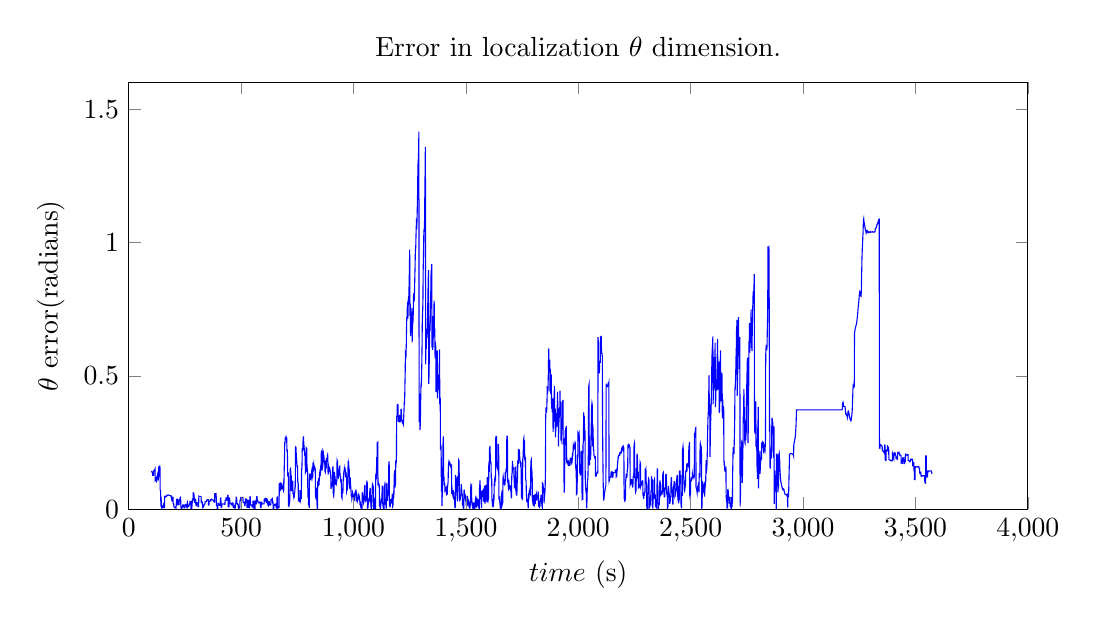
\begin{tikzpicture}

\begin{axis}[
title={Error in localization $\theta$ dimension.},
xlabel={$time$ (s)},
ylabel={$\theta$ error(radians)},
xmin=0, xmax=4000,
ymin=0, ymax=1.6,
axis on top,
width=13cm,
height=7cm
]
\addplot [blue]
coordinates {
(100,0.140530435246877)
(101,0.14121433894103)
(102,0.141176072759084)
(103,0.141051856679372)
(104,0.138091413182668)
(105,0.137415019673757)
(106,0.137637941045217)
(107,0.126923648518972)
(108,0.127199737233571)
(109,0.127156941098622)
(110,0.127174464864186)
(111,0.143673626584462)
(112,0.143880812329702)
(113,0.143165914220265)
(114,0.143111316365651)
(115,0.147231666249684)
(116,0.147402969998769)
(117,0.149654833478383)
(118,0.112180320424489)
(119,0.114739624661855)
(120,0.115592447919301)
(121,0.116502372426442)
(122,0.106330362958364)
(123,0.105422465009145)
(124,0.102535335225515)
(125,0.103065935773305)
(126,0.122217981023244)
(127,0.124929277104787)
(128,0.128443924588613)
(129,0.118756739301137)
(130,0.116743890447072)
(131,0.113351074857167)
(132,0.112063614530019)
(133,0.145282117528371)
(134,0.141422359151296)
(135,0.137618986768178)
(136,0.156390396756581)
(137,0.160184590024404)
(138,0.161189762753896)
(139,0.156449524564199)
(140,0.0726272741979876)
(141,0.070383993787221)
(142,0.065847245854787)
(143,0.0184995810217181)
(144,0.020389048261098)
(145,0.025441972417287)
(146,0.00664892991120425)
(147,0.00384977658326235)
(148,0.0068774541192731)
(149,0.00561645825440493)
(150,0.00712397893006411)
(151,0.00908163388306704)
(152,0.0111071189218244)
(153,0.009121449785777)
(154,0.0131230672174176)
(155,0.016459735231944)
(156,0.0123322327905377)
(157,0.0100562890344342)
(158,0.00656512578065005)
(159,0.00617888768250552)
(160,0.0483126958184918)
(161,0.048720272379466)
(162,0.0487659295373639)
(163,0.0468451102548322)
(164,0.0455996115976056)
(165,0.0458301623635968)
(166,0.0472743829065045)
(167,0.049039514856883)
(168,0.0490957816415509)
(169,0.049917610483714)
(170,0.0512761195474347)
(171,0.0505476315789899)
(172,0.05237069924409)
(173,0.0531825145059308)
(174,0.0531168301873883)
(175,0.053499849634715)
(176,0.0525634606652936)
(177,0.0526002963357648)
(178,0.0526461919122418)
(179,0.0516250451379499)
(180,0.0515064318948468)
(181,0.0512191375070294)
(182,0.0512531121545514)
(183,0.0510564168267926)
(184,0.0510450919442853)
(185,0.0506719668679914)
(186,0.050498517351695)
(187,0.0504118521981916)
(188,0.0503708442025861)
(189,0.0440330823236188)
(190,0.0438572486215314)
(191,0.0448249896341046)
(192,0.031259687738963)
(193,0.0301320870691022)
(194,0.0301760752969464)
(195,0.0301943143182477)
(196,0.0440793355279645)
(197,0.0442513545327863)
(198,0.021337477368764)
(199,0.0214976946539203)
(200,0.0215079466528216)
(201,0.00827184517914858)
(202,0.00766125519806948)
(203,0.00722649891907778)
(204,0.00703314145142642)
(205,0.00685158570344058)
(206,0.00752547581727114)
(207,0.00616660912568179)
(208,0.00510338147217837)
(209,0.0058102925592145)
(210,0.00364807446534243)
(211,0.0074659903817853)
(212,0.0248364527993878)
(213,0.0353652556710919)
(214,0.0349936803155622)
(215,0.0358226617150983)
(216,0.0173833688073834)
(217,0.0174786170297345)
(218,0.0170890410714826)
(219,0.0346939881616315)
(220,0.0335959513955792)
(221,0.0334095080667218)
(222,0.0193905512518207)
(223,0.0207384506887713)
(224,0.0199106613821307)
(225,0.0345630327886859)
(226,0.0356434265798846)
(227,0.0359929482168475)
(228,0.0360109488195697)
(229,0.0435083230310163)
(230,0.0447662194543561)
(231,0.0436724742227277)
(232,0.00911947886412534)
(233,0.00914212862913999)
(234,0.000344363851002782)
(235,5.89211755475105e-05)
(236,0.000363556546620458)
(237,0.0074035803503314)
(238,0.00782140891020688)
(239,0.00779208342497739)
(240,0.0153640190786639)
(241,0.0155416409200946)
(242,0.015232650441579)
(243,0.0154483000463763)
(244,0.0110679547018329)
(245,0.0107187906927386)
(246,0.00508805911009702)
(247,0.00475558440153989)
(248,0.00498649279539976)
(249,0.00479861895506772)
(250,0.0157410224252423)
(251,0.0158211310678205)
(252,0.0175208171182355)
(253,0.0174992402368268)
(254,0.0153594334893903)
(255,0.0133371671014508)
(256,0.0119742472940167)
(257,0.00875714619690982)
(258,0.00783959229523745)
(259,0.00579968293244448)
(260,0.0226434151357928)
(261,0.0248623768514911)
(262,0.00838848750059995)
(263,0.00937041441862974)
(264,0.00991043250029477)
(265,0.0101959387487689)
(266,0.010482517880849)
(267,0.011200873059682)
(268,0.0112970749563495)
(269,0.0196360667520246)
(270,0.0198337157540998)
(271,0.0182913859658917)
(272,0.0191403945260724)
(273,0.0291610638326922)
(274,0.0292386690801898)
(275,0.028245059651784)
(276,0.0281525532430926)
(277,0.000485150021962255)
(278,0.000606211023875147)
(279,0.000404683751515478)
(280,1.59422582903801e-05)
(281,0.0115598122305194)
(282,0.0116314570135394)
(283,0.0354494730657855)
(284,0.0351754109091083)
(285,0.034697024030141)
(286,0.0348363796896258)
(287,0.0608356873220721)
(288,0.0605834404653827)
(289,0.0604380051321307)
(290,0.0602366606420794)
(291,0.0329143683141986)
(292,0.0329488197988788)
(293,0.0273637453741351)
(294,0.025054780644826)
(295,0.0242299715704242)
(296,0.0364793221182147)
(297,0.0351216475195208)
(298,0.0339479128546039)
(299,0.0160139481252948)
(300,0.0142575184530536)
(301,0.0137824694341937)
(302,0.024227110547475)
(303,0.0239813009924212)
(304,0.0239247957891742)
(305,0.0234756151861468)
(306,0.0188664515786847)
(307,0.018889458971568)
(308,0.0095867792791644)
(309,0.0094787756628314)
(310,0.00952490965788755)
(311,0.00947007338469419)
(312,0.0480323712057391)
(313,0.046975700063161)
(314,0.048054424924306)
(315,0.0479472557729999)
(316,0.0479651371664325)
(317,0.0479938666052142)
(318,0.0478269735998431)
(319,0.0476331392950335)
(320,0.0474400202459613)
(321,0.0469225327200213)
(322,0.0466552654928485)
(323,0.0245241800970355)
(324,0.0242370049185077)
(325,0.0239241997427264)
(326,0.025640455884389)
(327,0.025742618245534)
(328,0.0261891762441913)
(329,0.00553855101530942)
(330,0.00597533385222349)
(331,0.00663861433928403)
(332,0.0102018992132464)
(333,0.0104061047262469)
(334,0.0106794516271869)
(335,0.0154753605551043)
(336,0.0162274519628802)
(337,0.0178185383505145)
(338,0.018292633695058)
(339,0.0189244429296771)
(340,0.0281016508764544)
(341,0.0282104889578143)
(342,0.0284123102850238)
(343,0.0284064690298358)
(344,0.0286549011892596)
(345,0.0286304632849017)
(346,0.0285855213827411)
(347,0.0322440544790545)
(348,0.0347866694158832)
(349,0.0349423567480365)
(350,0.0349135080999652)
(351,0.0345852057165423)
(352,0.0350169817632953)
(353,0.0348702351278583)
(354,0.0350391546911517)
(355,0.0152274052328387)
(356,0.0152831951803485)
(357,0.0153046528524676)
(358,0.0302391926473895)
(359,0.0301794687933246)
(360,0.0304307619756976)
(361,0.0307341496176043)
(362,0.0299743096060077)
(363,0.0301659981436053)
(364,0.0302495638555804)
(365,0.0357415358251849)
(366,0.0358314196295062)
(367,0.035738317174367)
(368,0.0351754109091083)
(369,0.037017671269826)
(370,0.0363465229696551)
(371,0.0359649340338031)
(372,0.0356524864858905)
(373,0.0350262800878802)
(374,0.0344506184286395)
(375,0.0342248360342303)
(376,0.0334555784887591)
(377,0.0325669924444476)
(378,0.0319640318578998)
(379,0.0269605795568744)
(380,0.0268485228246966)
(381,0.0266819874471942)
(382,0.0264002958959857)
(383,0.0576970259374896)
(384,0.057688681287221)
(385,0.0576042811102191)
(386,0.0576693693823138)
(387,0.0575712601370135)
(388,0.0575756708807269)
(389,0.0575587431616107)
(390,0.0135646740621844)
(391,0.0138706843084613)
(392,0.0139369646734515)
(393,0.0140555779165545)
(394,0.0021627267175397)
(395,0.00225725968415347)
(396,0.00243190129334536)
(397,0.0220304409689227)
(398,0.0217314640707293)
(399,0.0210946480459491)
(400,0.0211486498541156)
(401,0.0150245110220233)
(402,0.0148720423406878)
(403,0.0147176663107196)
(404,0.0146103779501239)
(405,0.0143793503469745)
(406,0.0144748369879046)
(407,0.0145046393102923)
(408,0.0410715023702899)
(409,0.0409989039129535)
(410,0.0414478460974017)
(411,0.00667270819609556)
(412,0.00705346266692075)
(413,0.00753137270872983)
(414,0.00796755949919614)
(415,0.0189325491613666)
(416,0.0192165056890765)
(417,0.0192837397283832)
(418,0.0192420164770404)
(419,0.0193999687856952)
(420,0.019527403516225)
(421,0.0196745077795306)
(422,0.0197418610281268)
(423,0.0198027769750873)
(424,0.0197549740499774)
(425,0.0198194662756244)
(426,0.0184272209829608)
(427,0.0184329430288592)
(428,0.0184414068884173)
(429,0.0326100269979754)
(430,0.0327068249410907)
(431,0.0327456871694842)
(432,0.0327281634039203)
(433,0.0419317166036883)
(434,0.0420410315222064)
(435,0.0421189943975726)
(436,0.041998950642995)
(437,0.0339325348562518)
(438,0.0338681618398944)
(439,0.034058539075307)
(440,0.0518054644293109)
(441,0.0517496744818011)
(442,0.0517762581533709)
(443,0.00839284260804263)
(444,0.00841942627961245)
(445,0.00870254834229556)
(446,0.00910106499726382)
(447,0.0418409983343402)
(448,0.0416748205847064)
(449,0.0413236300176898)
(450,0.0231578032202044)
(451,0.0227161328024188)
(452,0.0223190466589251)
(453,0.0219152847952166)
(454,0.0201392491632184)
(455,0.0205734093957624)
(456,0.0209160168939313)
(457,0.0159192959493915)
(458,0.01566228072112)
(459,0.0156097094244281)
(460,0.0154966990179339)
(461,0.0229229609197894)
(462,0.0229041258520404)
(463,0.0229258219427386)
(464,0.022932616872243)
(465,0.00675013859803286)
(466,0.00683608849579898)
(467,0.00684490998322573)
(468,0.0139590183920184)
(469,0.0139647404379168)
(470,0.0139586607641498)
(471,0.00429293314879331)
(472,0.00439199606841001)
(473,0.0041767040914813)
(474,0.0041079203314105)
(475,0.0203246752447406)
(476,0.020083872479848)
(477,0.0199761072820941)
(478,0.0445665995306292)
(479,0.0444577614492694)
(480,0.0443341414160052)
(481,0.0203864256567279)
(482,0.0200442949957171)
(483,0.0204373280233661)
(484,0.0205989758199969)
(485,0.0173797289556781)
(486,0.0175822655386249)
(487,0.0178036371893207)
(488,0.00340089003508481)
(489,0.00363406340544614)
(490,0.00396260420744809)
(491,0.0043215433782855)
(492,0.00473245779936704)
(493,0.00493868987028989)
(494,0.00533863703673276)
(495,0.0321556011862079)
(496,0.0322537104315082)
(497,0.0322746912664691)
(498,0.0436926762289325)
(499,0.0438557545370379)
(500,0.0439080874151507)
(501,0.0439823548025409)
(502,0.0439394394583026)
(503,0.0439253727621356)
(504,0.043891040486745)
(505,0.0438726822561541)
(506,0.0438415686315814)
(507,0.0438606421179095)
(508,0.0438372770971576)
(509,0.0246864239401141)
(510,0.0247380415624896)
(511,0.0248560587591449)
(512,0.0248818079656878)
(513,0.0249166170782367)
(514,0.0249362866110125)
(515,0.0249429623312274)
(516,0.0130855719274798)
(517,0.0131212155050555)
(518,0.01330312888091)
(519,0.03810969193513)
(520,0.0379144271188459)
(521,0.03797701199586)
(522,0.037978084879466)
(523,0.0367690006918231)
(524,0.0366733948416034)
(525,0.0365491787618915)
(526,0.0078317801183978)
(527,0.00762721697752866)
(528,0.00739797751372251)
(529,0.0065960009866437)
(530,0.00675550301606265)
(531,0.00691285927826968)
(532,0.0326329151815692)
(533,0.0324951092428485)
(534,0.032321421307973)
(535,0.0321148316091815)
(536,0.00538381735747251)
(537,0.00511428515379819)
(538,0.00495359103148374)
(539,0.0461758057302752)
(540,0.0461182276434222)
(541,0.0461355129904071)
(542,0.0155768076605121)
(543,0.0155856291479388)
(544,0.0156030337042132)
(545,0.0156533400244037)
(546,0.0155347267813006)
(547,0.0155222098058978)
(548,0.0155467669195453)
(549,0.0081678946786603)
(550,0.00819638569886294)
(551,0.00817302067811099)
(552,0.00818684895569888)
(553,0.0299405733770648)
(554,0.0298370997137347)
(555,0.0297457853979388)
(556,0.0297044197744647)
(557,0.000894816713877589)
(558,0.00102809269959536)
(559,0.00111130078370181)
(560,0.00107374985749331)
(561,0.00121882756287661)
(562,0.00119164784485903)
(563,0.0306927839941302)
(564,0.0308276097006122)
(565,0.0309948603338519)
(566,0.0200057903951922)
(567,0.0202599446005145)
(568,0.0203019062704364)
(569,0.0462543646520892)
(570,0.0464628616995135)
(571,0.0466885248846332)
(572,0.0302289406484881)
(573,0.0303004662222186)
(574,0.0305821577734271)
(575,0.0305155197805682)
(576,0.0233182589239398)
(577,0.02337392966216)
(578,0.0235454718298236)
(579,0.0238825957006732)
(580,0.0239529291815082)
(581,0.0236490647024432)
(582,0.024019567174367)
(583,0.0266285816854754)
(584,0.0264937559789935)
(585,0.0264365355200091)
(586,0.00611099402373227)
(587,0.0059934536642352)
(588,0.00594231287901792)
(589,0.00600835482542905)
(590,0.0257396380132953)
(591,0.0257305781072894)
(592,0.0257926861471454)
(593,0.0192463080114642)
(594,0.0193710009283343)
(595,0.0193156878179828)
(596,0.0193603913015643)
(597,0.0194760243124286)
(598,0.0194940249151507)
(599,0.0195159594244281)
(600,0.0195580403036395)
(601,0.0195578018850604)
(602,0.0196220556921283)
(603,0.0379277149862567)
(604,0.0381501595205584)
(605,0.0380224863714496)
(606,0.0379235426611224)
(607,0.0303936878866473)
(608,0.0302891413397113)
(609,0.0406320969290057)
(610,0.0405420939153949)
(611,0.0404423157400409)
(612,0.0402002016729632)
(613,0.0244621912664691)
(614,0.0242626349157611)
(615,0.0241248289770404)
(616,0.0373404900259295)
(617,0.0371902863210956)
(618,0.0367936770147601)
(619,0.0147345940298358)
(620,0.0146763006872455)
(621,0.0135881582922259)
(622,0.0281889120764056)
(623,0.0282196680731097)
(624,0.0282146612829486)
(625,0.0281612555212298)
(626,0.0156826655096332)
(627,0.0155284086889544)
(628,0.015461651486806)
(629,0.0155560652441302)
(630,0.0163389126486102)
(631,0.0164701620764056)
(632,0.0173734108633319)
(633,0.0355167071050921)
(634,0.0365687290853778)
(635,0.0357000509924212)
(636,0.0366007963842669)
(637,0.0353560129827777)
(638,0.036370960874013)
(639,0.0378311554617206)
(640,0.0242182334237775)
(641,0.0247022231393537)
(642,0.0253728946023664)
(643,0.00292983849579898)
(644,0.00331106980378237)
(645,0.0030862410836896)
(646,0.0133933146768292)
(647,0.0142759402566632)
(648,0.0159544070535382)
(649,0.0148698409372052)
(650,0.0161083062463483)
(651,0.0177066644006452)
(652,0.0171820243173322)
(653,0.017799051600047)
(654,0.0188535769754132)
(655,0.0194230397515973)
(656,0.0046494881338397)
(657,0.00411245028441343)
(658,0.00402256648009214)
(659,0.00421878497069272)
(660,0.0432836691564837)
(661,0.0428435484594623)
(662,0.0440488735861102)
(663,0.00436112086241636)
(664,0.00520321528380308)
(665,0.00594076315825376)
(666,0.00556906859343442)
(667,0.00644656817381772)
(668,0.00564273993437681)
(669,0.00663611094420347)
(670,0.0962900797552386)
(671,0.096194712323598)
(672,0.0957518498129168)
(673,0.0966999212927142)
(674,0.0726735274023333)
(675,0.0741814057058612)
(676,0.0731279532141009)
(677,0.094483343762807)
(678,0.0957109610266009)
(679,0.0954318920797625)
(680,0.0767289082235614)
(681,0.0774910132116595)
(682,0.0782333294576922)
(683,0.0797136704153338)
(684,0.0824900547689715)
(685,0.085204927129201)
(686,0.0888464132971087)
(687,0.0697741190618792)
(688,0.0758951584524432)
(689,0.0690790096945086)
(690,0.0718859116262713)
(691,0.112080542249135)
(692,0.156259147328786)
(693,0.189607588452748)
(694,0.252140728635244)
(695,0.246959535283498)
(696,0.256328789395742)
(697,0.270223585767202)
(698,0.270297376317433)
(699,0.26789411704009)
(700,0.258793441457204)
(701,0.268606750173024)
(702,0.26558789412444)
(703,0.265628782910756)
(704,0.217486230534963)
(705,0.2177470604605)
(706,0.218786803883962)
(707,0.125255672139577)
(708,0.124621359509877)
(709,0.129412857694081)
(710,0.138054577512197)
(711,0.00918582280213442)
(712,0.0145173390680036)
(713,0.0249924977594098)
(714,0.0173825343423566)
(715,0.0217628796869)
(716,0.0294105132394513)
(717,0.0297305901818952)
(718,0.148032816248485)
(719,0.150759967165538)
(720,0.152028592424937)
(721,0.137557061510631)
(722,0.119292291002818)
(723,0.120470197992869)
(724,0.0676954110437116)
(725,0.0761598666482648)
(726,0.0827414115243634)
(727,0.0850445349984845)
(728,0.10032573540742)
(729,0.103677900629588)
(730,0.102725895243235)
(731,0.0596143325143537)
(732,0.0600673278146466)
(733,0.0559041817956647)
(734,0.0479259808831891)
(735,0.0420816262536725)
(736,0.0437931140237531)
(737,0.0523524602227887)
(738,0.0627239068322858)
(739,0.0653791745477399)
(740,0.0817801078134259)
(741,0.083154710131236)
(742,0.232515247660228)
(743,0.233569892244883)
(744,0.232258828478404)
(745,0.212584884958812)
(746,0.194875510531016)
(747,0.190410049753734)
(748,0.162735017138072)
(749,0.162702949839183)
(750,0.15637460549409)
(751,0.164498003321238)
(752,0.102963360148021)
(753,0.0986997206979474)
(754,0.0970666726403913)
(755,0.033716233568736)
(756,0.0349412282281598)
(757,0.0335634072595319)
(758,0.0360371192270001)
(759,0.0322969834036151)
(760,0.0359971205419818)
(761,0.028031436604909)
(762,0.0707583109564105)
(763,0.061243859929494)
(764,0.0582216660208026)
(765,0.0377794186300555)
(766,0.0428597052865705)
(767,0.041659029322215)
(768,0.0412735064798078)
(769,0.140661509829112)
(770,0.151689561205455)
(771,0.163622887926646)
(772,0.225956233339854)
(773,0.227796943979808)
(774,0.228198560076304)
(775,0.227091463404246)
(776,0.267513068514415)
(777,0.269880207377025)
(778,0.270596655207225)
(779,0.232909591990062)
(780,0.235950263338633)
(781,0.226208718615123)
(782,0.218143733339854)
(783,0.202114017801829)
(784,0.200864227610179)
(785,0.202722581224986)
(786,0.142135175066539)
(787,0.145889671640941)
(788,0.140004547434398)
(789,0.141910942392894)
(790,0.22938314278657)
(791,0.228390367823192)
(792,0.226076157885142)
(793,0.167410524683543)
(794,0.154050501185008)
(795,0.144918950396129)
(796,0.137131365137645)
(797,0.0616554339700421)
(798,0.0658160765939435)
(799,0.0679148753457746)
(800,0.0159753878884992)
(801,0.0157288630777082)
(802,0.0246365388208112)
(803,0.00438746611540708)
(804,0.123466761904307)
(805,0.121342094736644)
(806,0.130878003435679)
(807,0.130643280344554)
(808,0.11850634415681)
(809,0.116491707163402)
(810,0.108465703325816)
(811,0.117349418001719)
(812,0.118576200800486)
(813,0.132182272272654)
(814,0.143042119341441)
(815,0.147688182192393)
(816,0.1417819579416)
(817,0.121131451922007)
(818,0.125961931543895)
(819,0.124829443293162)
(820,0.173981698351451)
(821,0.162668736773082)
(822,0.164589675264903)
(823,0.169429691629954)
(824,0.150349768000194)
(825,0.152551563578196)
(826,0.158138545351573)
(827,0.159186156588145)
(828,0.157294185953685)
(829,0.152660640078135)
(830,0.149238499003001)
(831,0.0522389729791364)
(832,0.0479784329705915)
(833,0.0380995591455182)
(834,0.0377416928582868)
(835,0.071823390322276)
(836,0.0769695361428937)
(837,0.0760352929406842)
(838,0.00987610022490415)
(839,0.00300988356535825)
(840,0.000820724172047704)
(841,0.0993383248620709)
(842,0.0986415465646466)
(843,0.104009779291697)
(844,0.0987038930230817)
(845,0.0993206818872174)
(846,0.0910058339410504)
(847,0.0918824990564069)
(848,0.120513709383555)
(849,0.132033737497874)
(850,0.137551458674022)
(851,0.131681116419383)
(852,0.137896450357982)
(853,0.135594518976756)
(854,0.161744268732615)
(855,0.163408311205455)
(856,0.168016823130198)
(857,0.220305236177989)
(858,0.210833700495311)
(859,0.209595950441905)
(860,0.144975932436534)
(861,0.15145197709138)
(862,0.155383261042186)
(863,0.157881649332591)
(864,0.219865949945994)
(865,0.217851551371165)
(866,0.213953646021434)
(867,0.184455784159251)
(868,0.188536079721995)
(869,0.191363485651561)
(870,0.18039861519868)
(871,0.179378541307994)
(872,0.179808648424693)
(873,0.147576244669505)
(874,0.14963427384431)
(875,0.144669922190257)
(876,0.156697424250194)
(877,0.172003420191356)
(878,0.169493826227733)
(879,0.165811808901378)
(880,0.189974101381846)
(881,0.19017210801179)
(882,0.185693176584788)
(883,0.177705915766307)
(884,0.200531395273753)
(885,0.20368483861024)
(886,0.196049722033091)
(887,0.130031975107737)
(888,0.138651521997996)
(889,0.13998523552949)
(890,0.156988890963145)
(891,0.152002008753367)
(892,0.1494404395395)
(893,0.148715170221873)
(894,0.151301892595836)
(895,0.145214947062083)
(896,0.146150620775767)
(897,0.134689005213328)
(898,0.126441510515757)
(899,0.120900305109569)
(900,0.0765072425180158)
(901,0.0825215895944318)
(902,0.0867971499734601)
(903,0.0859930833154401)
(904,0.0972200949960431)
(905,0.0964875539117536)
(906,0.0997696240716657)
(907,0.151102693872996)
(908,0.14854362805421)
(909,0.150743277865001)
(910,0.0599582513147077)
(911,0.0517423470788678)
(912,0.0484794696145734)
(913,0.0559454282098493)
(914,0.136644991236277)
(915,0.13713804085786)
(916,0.133618028956004)
(917,0.105985434847423)
(918,0.103261740999766)
(919,0.107892425852366)
(920,0.0940839370065412)
(921,0.0945766290002545)
(922,0.0988278706842145)
(923,0.101344617205211)
(924,0.0966812690072736)
(925,0.101660760241099)
(926,0.113121183710643)
(927,0.183961661654063)
(928,0.181338222818919)
(929,0.178596528368541)
(930,0.12347653706605)
(931,0.119674237566539)
(932,0.117949517565318)
(933,0.116782577829905)
(934,0.137223037081309)
(935,0.143203171091624)
(936,0.136173637705394)
(937,0.155515344935008)
(938,0.16052511532838)
(939,0.161032350855418)
(940,0.127787144976207)
(941,0.126342328386851)
(942,0.123941691713878)
(943,0.113174589472361)
(944,0.0996243079477033)
(945,0.0993429740243634)
(946,0.101598413782664)
(947,0.0477496703439435)
(948,0.0437516291909894)
(949,0.041372688608714)
(950,0.0633999427133283)
(951,0.0656527598672589)
(952,0.0643090327554425)
(953,0.0634800513559064)
(954,0.118900807695933)
(955,0.113690527277537)
(956,0.10386327107484)
(957,0.139526875811168)
(958,0.141778500872203)
(959,0.150075825052806)
(960,0.142202289896556)
(961,0.141723187761851)
(962,0.14774218400056)
(963,0.151279123621531)
(964,0.148627312975474)
(965,0.121986897783824)
(966,0.121323974924632)
(967,0.139836104708262)
(968,0.124542148905345)
(969,0.123095186548777)
(970,0.0692318995767316)
(971,0.0736991484933576)
(972,0.0731450637155255)
(973,0.0876380523019513)
(974,0.0936237891488751)
(975,0.0964622815423688)
(976,0.17160406907136)
(977,0.169851334887095)
(978,0.174260886507579)
(979,0.160492928820201)
(980,0.15067723591859)
(981,0.148285182314464)
(982,0.0771034081750592)
(983,0.0835659821801862)
(984,0.0801743586831769)
(985,0.0814119895272931)
(986,0.119450600939341)
(987,0.0861842950158795)
(988,0.0838063081079206)
(989,0.0690305550866803)
(990,0.053288610773631)
(991,0.0441825707727155)
(992,0.0535616000467023)
(993,0.038562687235423)
(994,0.0427469332986554)
(995,0.0516659339242658)
(996,0.0449425299936017)
(997,0.0569711049371442)
(998,0.052003415422984)
(999,0.0506817420297345)
(1000,0.0468534549051007)
(1001,0.0490765889459333)
(1002,0.0507966597848615)
(1003,0.0384996255212506)
(1004,0.0335825999551496)
(1005,0.0335423072152814)
(1006,0.0605868418985089)
(1007,0.0616450627618512)
(1008,0.0573807080560407)
(1009,0.0600816329293927)
(1010,0.0710445960336408)
(1011,0.0710962136560163)
(1012,0.067268045740672)
(1013,0.0367131551080426)
(1014,0.0397538264566144)
(1015,0.0362260659509381)
(1016,0.0353247245126447)
(1017,0.0350940545373639)
(1018,0.0317144711785993)
(1019,0.0425298531823834)
(1020,0.0378543456369123)
(1021,0.039819749193736)
(1022,0.0478868802362165)
(1023,0.0421629269891461)
(1024,0.0390521605783185)
(1025,0.0395162423425397)
(1026,0.0457097609811505)
(1027,0.0415468533807477)
(1028,0.0310551245980939)
(1029,0.0182804187112531)
(1030,0.0184628089242658)
(1031,0.0280896743112287)
(1032,0.00893685023253354)
(1033,0.00832792918150815)
(1034,0.00305155118043032)
(1035,0.00962773163849917)
(1036,0.00637927849824038)
(1037,0.00856653054291812)
(1038,0.00683120091492739)
(1039,0.0623805840783795)
(1040,0.053786190348216)
(1041,0.0416604598336896)
(1042,0.0478319247537335)
(1043,0.0398367961221417)
(1044,0.0371412356668195)
(1045,0.0263518412881574)
(1046,0.0308219512277326)
(1047,0.04344895680482)
(1048,0.0419332106881818)
(1049,0.0802762826257428)
(1050,0.0853445847802838)
(1051,0.090913327532359)
(1052,0.0505060275369367)
(1053,0.0325093587213239)
(1054,0.0349696000390729)
(1055,0.0350793917947492)
(1056,0.0436686595254621)
(1057,0.0315958579354962)
(1058,0.0318121035867414)
(1059,0.099076660471507)
(1060,0.102452429133006)
(1061,0.0996285994821271)
(1062,0.00155600706999692)
(1063,0.0117029269509992)
(1064,0.0104084332757672)
(1065,0.00386461417143735)
(1066,0.0336237271600446)
(1067,0.0348625500970563)
(1068,0.0271348079019269)
(1069,0.0418473799997052)
(1070,0.0309695323281964)
(1071,0.038174184160777)
(1072,0.0526852925592145)
(1073,0.0742638428979596)
(1074,0.0769584496789655)
(1075,0.0766129811578473)
(1076,0.0242138226800641)
(1077,0.0220088084512433)
(1078,0.00778690178925601)
(1079,0.00183311303193179)
(1080,0.00163659254973325)
(1081,0.00972143014008608)
(1082,0.0177039225869855)
(1083,0.0744514783197125)
(1084,0.0910451730066022)
(1085,0.0937751849466046)
(1086,0.088753493624278)
(1087,0.0884917100244245)
(1088,0.0816514809900006)
(1089,0.0799018462472638)
(1090,0.000271169347218603)
(1091,0.000508459406443507)
(1092,0.00962838332121763)
(1093,0.0357810576730451)
(1094,0.0325763543420514)
(1095,0.0322773774438581)
(1096,0.0102422555261334)
(1097,0.0107115824990949)
(1098,0.00071939627592954)
(1099,0.127071110410146)
(1100,0.130584923428945)
(1101,0.113517729443959)
(1102,0.115092841786794)
(1103,0.182507960004262)
(1104,0.179638950032643)
(1105,0.178431955975942)
(1106,0.252932874364308)
(1107,0.236372200650624)
(1108,0.23974630038207)
(1109,0.0984786431021014)
(1110,0.100809542340688)
(1111,0.0974492708868304)
(1112,0.097835508984975)
(1113,0.0880274454778949)
(1114,0.0828276554769793)
(1115,0.0920421759313861)
(1116,0.00955220858519468)
(1117,0.0163930336660663)
(1118,0.0158562342352191)
(1119,0.00171157519286069)
(1120,0.00526014168793765)
(1121,0.0133695920282086)
(1122,0.0148697217279157)
(1123,0.0372715314202985)
(1124,0.0377497990899762)
(1125,0.0333812554650983)
(1126,0.0371703227334699)
(1127,0.0567774454778949)
(1128,0.0863120238012591)
(1129,0.086334077519826)
(1130,0.0224215666479388)
(1131,0.0172136704153338)
(1132,0.00502630869810972)
(1133,0.00308856169646177)
(1134,0.00454482237761411)
(1135,0.00334843794768247)
(1136,0.00137159029906186)
(1137,0.0829281489080707)
(1138,0.0862816254324237)
(1139,0.0905278603262225)
(1140,0.017080156011037)
(1141,0.0349222103781024)
(1142,0.0306650082296649)
(1143,0.0293543020910541)
(1144,0.0229704062170306)
(1145,0.00915071169798765)
(1146,0.00240561167662534)
(1147,0.0886510928445539)
(1148,0.0858400185876569)
(1149,0.0883127768808087)
(1150,0.0420074145025531)
(1151,0.0307128111547748)
(1152,0.0438137928671161)
(1153,0.0625679175085345)
(1154,0.0595247427648822)
(1155,0.0578087250417987)
(1156,0.051998106641225)
(1157,0.164944974584035)
(1158,0.178740111989431)
(1159,0.161817042035512)
(1160,0.0125101486868182)
(1161,0.0191341320699969)
(1162,0.0129211823171893)
(1163,0.00633212725584897)
(1164,0.0186901966757098)
(1165,0.0268554369634906)
(1166,0.0370255390829364)
(1167,0.0244555791192731)
(1168,0.0240463336282453)
(1169,0.0331544001870832)
(1170,0.0398334582620343)
(1171,0.0252454598718366)
(1172,0.0465519746118268)
(1173,0.0578370412164411)
(1174,0.00974372227723208)
(1175,0.0116867144876203)
(1176,0.0203180630975446)
(1177,0.0432063023275653)
(1178,0.0445556322759906)
(1179,0.0607539097494403)
(1180,0.0574583689398089)
(1181,0.126859156293325)
(1182,0.133899776143483)
(1183,0.137356487912587)
(1184,0.146041838330678)
(1185,0.0968752781576434)
(1186,0.0900869051641742)
(1187,0.094027964276723)
(1188,0.172171203298024)
(1189,0.169826952619008)
(1190,0.175843445462636)
(1191,0.177440730733327)
(1192,0.347697703046254)
(1193,0.349214879674367)
(1194,0.348540631932668)
(1195,0.391831962270192)
(1196,0.390944329900197)
(1197,0.391443101567678)
(1198,0.390781490010671)
(1199,0.330249993009023)
(1200,0.329567042989186)
(1201,0.330916372937612)
(1202,0.329835979146413)
(1203,0.329017249745778)
(1204,0.349237767857961)
(1205,0.350326148671559)
(1206,0.349178878468923)
(1207,0.32802948157256)
(1208,0.328012673062734)
(1209,0.327912298840932)
(1210,0.327810136479787)
(1211,0.370743004483632)
(1212,0.369614092511586)
(1213,0.370894042653493)
(1214,0.333513943356923)
(1215,0.333676306409291)
(1216,0.333770600957326)
(1217,0.33380660216277)
(1218,0.322574345273427)
(1219,0.322272626561574)
(1220,0.320959178609304)
(1221,0.318514911336354)
(1222,0.316465346021108)
(1223,0.336512533826284)
(1224,0.357429711026601)
(1225,0.378645030660085)
(1226,0.398931829137258)
(1227,0.398169008893422)
(1228,0.424784866971425)
(1229,0.473143307370595)
(1230,0.509004441899709)
(1231,0.581649867696218)
(1232,0.577765671414785)
(1233,0.564030377072744)
(1234,0.587471095723561)
(1235,0.618911592168264)
(1236,0.679313031835012)
(1237,0.714048711461476)
(1238,0.714816776914052)
(1239,0.743607966107778)
(1240,0.739116398496083)
(1241,0.776841131848744)
(1242,0.713983265561513)
(1243,0.74367090861266)
(1244,0.791066376370839)
(1245,0.76907488505309)
(1246,0.795579640073232)
(1247,0.82323166529601)
(1248,0.864679543179921)
(1249,0.90692946116393)
(1250,0.972969261807851)
(1251,0.733259765309743)
(1252,0.734973518056325)
(1253,0.770613280934743)
(1254,0.648611990613393)
(1255,0.674668757123403)
(1256,0.690988032025746)
(1257,0.697776762647084)
(1258,0.698619333905629)
(1259,0.724662748975209)
(1260,0.75430175463622)
(1261,0.625316886109761)
(1262,0.661913661164693)
(1263,0.700969247025899)
(1264,0.692547110719136)
(1265,0.710767773789815)
(1266,0.73715212742751)
(1267,0.791391400498799)
(1268,0.80869868199294)
(1269,0.781559733552388)
(1270,0.781172064942769)
(1271,0.797480611009053)
(1272,0.835527447862081)
(1273,0.874645499391011)
(1274,0.908089903993062)
(1275,0.955449434118815)
(1276,0.975683065252849)
(1277,0.979829402762004)
(1278,1.02159843047196)
(1279,1.04947599967057)
(1280,1.07598361571366)
(1281,1.07209095557267)
(1282,1.06708130438859)
(1283,1.0854783972078)
(1284,1.13744673331315)
(1285,1.17578014929826)
(1286,1.24276742537553)
(1287,1.29227981169755)
(1288,1.30700931151445)
(1289,1.31573781569535)
(1290,1.35472354491288)
(1291,1.41599282820756)
(1292,0.326205523806163)
(1293,0.378925355272838)
(1294,0.417823823290416)
(1295,0.432726891832896)
(1296,0.296172859268733)
(1297,0.315509559708186)
(1298,0.355784418182918)
(1299,0.410084279375621)
(1300,0.450476678209849)
(1301,0.476681979494639)
(1302,0.461171658831187)
(1303,0.503081353502818)
(1304,0.547364505129405)
(1305,0.603297503786631)
(1306,0.69119122822816)
(1307,0.724010976152965)
(1308,0.745999368029185)
(1309,0.784251006441661)
(1310,0.893541010218211)
(1311,0.934385212259837)
(1312,0.981714638071605)
(1313,1.03465858300263)
(1314,1.0497831424051)
(1315,1.03979686101014)
(1316,1.06657913525636)
(1317,1.15507891972596)
(1318,1.20071008999879)
(1319,1.31693735917146)
(1320,1.35856834252412)
(1321,0.54261842568452)
(1322,0.605387004213878)
(1323,0.62370744545991)
(1324,0.601423891382762)
(1325,0.643455894785472)
(1326,0.676526101427623)
(1327,0.642214687662669)
(1328,0.657384665804454)
(1329,0.685251625376292)
(1330,0.746768863993235)
(1331,0.78701630433137)
(1332,0.841102035837718)
(1333,0.875348957377025)
(1334,0.896402986841746)
(1335,0.470167191820689)
(1336,0.501711042719432)
(1337,0.552005620794841)
(1338,0.622517915564128)
(1339,0.670019062357493)
(1340,0.685453267889567)
(1341,0.682352217035838)
(1342,0.735314043360301)
(1343,0.778199346857615)
(1344,0.819652767973491)
(1345,0.877306671934672)
(1346,0.893235536413737)
(1347,0.889898153143474)
(1348,0.91917213995988)
(1349,0.606164904432841)
(1350,0.655341597395488)
(1351,0.724225701885768)
(1352,0.597571076946803)
(1353,0.618781747417994)
(1354,0.616670074062892)
(1355,0.654611768322535)
(1356,0.664399804668971)
(1357,0.70833200414712)
(1358,0.7585932632261)
(1359,0.782298030453273)
(1360,0.659282388287135)
(1361,0.646871270733424)
(1362,0.676751317577907)
(1363,0.565859498577662)
(1364,0.625489005009182)
(1365,0.620314368168362)
(1366,0.609099635044583)
(1367,0.43913341418887)
(1368,0.489351520436355)
(1369,0.53604198445613)
(1370,0.523489954071589)
(1371,0.561729313927241)
(1372,0.588543297844478)
(1373,0.594854356842585)
(1374,0.415298702316829)
(1375,0.4415966292196)
(1376,0.504737617569514)
(1377,0.454963090019771)
(1378,0.456472398834773)
(1379,0.448402287560054)
(1380,0.475239636498042)
(1381,0.507172467308589)
(1382,0.557502629356929)
(1383,0.599208744364329)
(1384,0.393713084859304)
(1385,0.41406258742278)
(1386,0.414261905354909)
(1387,0.224125472707204)
(1388,0.223495570821218)
(1389,0.22585686842864)
(1390,0.228066054982595)
(1391,0.0743027607626239)
(1392,0.07631262938445)
(1393,0.0760312954611102)
(1394,0.0110986550622663)
(1395,0.0622979680723468)
(1396,0.0633393804258624)
(1397,0.116192011041097)
(1398,0.233851043385915)
(1399,0.260343877477101)
(1400,0.272566703957967)
(1401,0.107539204759053)
(1402,0.107831386727742)
(1403,0.110647288960866)
(1404,0.0929813663191119)
(1405,0.0939851085371295)
(1406,0.093745617074422)
(1407,0.0674727837271014)
(1408,0.0686526576704303)
(1409,0.0705237666792193)
(1410,0.0698555390066424)
(1411,0.078378287953786)
(1412,0.0803882161802569)
(1413,0.0817043463415423)
(1414,0.0533850471205035)
(1415,0.0536064783758441)
(1416,0.0555753986067096)
(1417,0.0570959130949298)
(1418,0.0876331607527057)
(1419,0.0869272629446307)
(1420,0.0953031460470477)
(1421,0.102444438142232)
(1422,0.144286958379201)
(1423,0.169119207066945)
(1424,0.16471275488799)
(1425,0.164854375523976)
(1426,0.167450396222524)
(1427,0.170810548467092)
(1428,0.174836484593801)
(1429,0.171254960698537)
(1430,0.168389884633473)
(1431,0.165696112317494)
(1432,0.166726199788503)
(1433,0.159497706098012)
(1434,0.155737606687001)
(1435,0.160942880315236)
(1436,0.162344662351064)
(1437,0.057773081464223)
(1438,0.0655109564489642)
(1439,0.0729233900732318)
(1440,0.0644018332189837)
(1441,0.0623849312490741)
(1442,0.0510402599996844)
(1443,0.0476464907354632)
(1444,0.0707027594274798)
(1445,0.0596110502905169)
(1446,0.0607654730505267)
(1447,0.0450600703530988)
(1448,0.0449314435296735)
(1449,0.0442555268579206)
(1450,0.0372457822137555)
(1451,0.00614491303498355)
(1452,0.0060232003503522)
(1453,0.00594058831269351)
(1454,0.127952663106374)
(1455,0.12082585493987)
(1456,0.119900671643666)
(1457,0.116123286885671)
(1458,0.0829311291403094)
(1459,0.0874621550268451)
(1460,0.0920067707723895)
(1461,0.0373489538854876)
(1462,0.0350526253408709)
(1463,0.0416130701727191)
(1464,0.114221183461598)
(1465,0.111826626462392)
(1466,0.112186161679677)
(1467,0.110055057210378)
(1468,0.185040561360768)
(1469,0.18365499178832)
(1470,0.179962722463063)
(1471,0.03410550753539)
(1472,0.0356541554159442)
(1473,0.0379621664709369)
(1474,0.0348530689901629)
(1475,0.0368226448721209)
(1476,0.0432066599554339)
(1477,0.0530150810903827)
(1478,0.0544479767507831)
(1479,0.0937932411855975)
(1480,0.0878704468435565)
(1481,0.0802553574270526)
(1482,0.0621043125814715)
(1483,0.054267017049245)
(1484,0.054243652028493)
(1485,0.016247185068675)
(1486,0.0154297669702252)
(1487,0.0209855159097394)
(1488,0.00918880303437319)
(1489,0.00202640692656431)
(1490,0.0037649552053729)
(1491,0.00282105605070981)
(1492,0.0736503283209125)
(1493,0.0686646382040301)
(1494,0.0608768145269671)
(1495,0.0491827408499041)
(1496,0.0414449850744525)
(1497,0.0417298952764789)
(1498,0.0452905575460711)
(1499,0.0371622165017804)
(1500,0.0399974902444562)
(1501,0.0363403876596173)
(1502,0.0115526040368756)
(1503,0.0112749656015119)
(1504,0.0124770720773419)
(1505,0.0200150330835065)
(1506,0.0477742830938617)
(1507,0.0475030819601336)
(1508,0.0403577963537494)
(1509,0.0201497952169696)
(1510,0.0221807638830462)
(1511,0.0230128447241107)
(1512,0.0286243279748639)
(1513,0.0251270850473126)
(1514,0.00932494004304019)
(1515,0.00767687161500064)
(1516,0.00908943812315854)
(1517,0.00689169566100034)
(1518,0.00259259541565982)
(1519,0.0228402296728412)
(1520,0.0307608524984637)
(1521,0.0274349133199969)
(1522,0.0858662446313581)
(1523,0.0826624949746808)
(1524,0.0862434228234967)
(1525,0.0881413539224347)
(1526,0.037853630381175)
(1527,0.026805194216319)
(1528,0.0250753482156476)
(1529,0.0134421269125262)
(1530,0.00925311247771177)
(1531,0.0155225674337665)
(1532,0.0182195584005633)
(1533,0.00705393950407895)
(1534,0.00245615641539487)
(1535,0.00253471533720884)
(1536,0.017411621409007)
(1537,0.0189956744485578)
(1538,0.0208143313699445)
(1539,0.00572231610352603)
(1540,0.00836983521515933)
(1541,0.00918141205842105)
(1542,0.0123215039544782)
(1543,0.0386365334219256)
(1544,0.0353549400991717)
(1545,0.0367043892568866)
(1546,0.0319760719961444)
(1547,0.0110662857717791)
(1548,0.0132169405645648)
(1549,0.0155146996206561)
(1550,0.0383173545175275)
(1551,0.0356259663873395)
(1552,0.0245272239022931)
(1553,0.021397741633006)
(1554,0.0165933688455304)
(1555,0.021414192514964)
(1556,0.0362956841760358)
(1557,0.0126296599679669)
(1558,0.010836275415965)
(1559,0.00347045262391177)
(1560,0.00161555607850161)
(1561,0.0907245000177106)
(1562,0.0909266789727887)
(1563,0.10741380055482)
(1564,0.0816924889856061)
(1565,0.0664389451318463)
(1566,0.0563571770959577)
(1567,0.0537544806771955)
(1568,0.0218715349859515)
(1569,0.0173631588644305)
(1570,0.00402995745604429)
(1571,0.0693023522668561)
(1572,0.0487892945581159)
(1573,0.0468967278772077)
(1574,0.0473525842004499)
(1575,0.0548456033044538)
(1576,0.0702393372827252)
(1577,0.0715220292382917)
(1578,0.0500443299585065)
(1579,0.040986569719859)
(1580,0.0276637395196637)
(1581,0.0684536377615252)
(1582,0.0777436176962176)
(1583,0.0844781080908099)
(1584,0.0852789560980121)
(1585,0.0210005919164935)
(1586,0.0291036049551288)
(1587,0.0339181105322162)
(1588,0.0784006993002215)
(1589,0.0847030560201922)
(1590,0.0906382481283465)
(1591,0.0393316427892962)
(1592,0.0377839485830584)
(1593,0.0336590687460223)
(1594,0.0252698342031756)
(1595,0.119715897244863)
(1596,0.109569756192617)
(1597,0.109943834943227)
(1598,0.115130511922292)
(1599,0.053825704259328)
(1600,0.0383189598745624)
(1601,0.0429389158911029)
(1602,0.162152377767018)
(1603,0.158667890233449)
(1604,0.155367581052236)
(1605,0.225587574643544)
(1606,0.225536076230458)
(1607,0.23745080630248)
(1608,0.216313449544362)
(1609,0.177528707189015)
(1610,0.178784338635854)
(1611,0.178701368970327)
(1612,0.168726412457875)
(1613,0.115963904065541)
(1614,0.114717451733998)
(1615,0.113007275266103)
(1616,0.0373645703024188)
(1617,0.0281003395742694)
(1618,0.0341012160009662)
(1619,0.0196587721533099)
(1620,0.0156089941686908)
(1621,0.00934907595580015)
(1622,0.0103380362219134)
(1623,0.0345230420404157)
(1624,0.0303778966241559)
(1625,0.0368328412347516)
(1626,0.0912568251318255)
(1627,0.0997821966833392)
(1628,0.0928461233801166)
(1629,0.0870077292150775)
(1630,0.126951185864858)
(1631,0.119437662763051)
(1632,0.117247072858266)
(1633,0.265803066892079)
(1634,0.272219864530019)
(1635,0.272857395810536)
(1636,0.272669998807363)
(1637,0.163686005277089)
(1638,0.164389816922597)
(1639,0.166942326230458)
(1640,0.152565924329213)
(1641,0.150962797803334)
(1642,0.151085821790151)
(1643,0.147346464795522)
(1644,0.244617668790273)
(1645,0.232363430661611)
(1646,0.210477677983693)
(1647,0.0433194955163678)
(1648,0.0364959557824811)
(1649,0.0365536530786237)
(1650,0.047531398134776)
(1651,0.0247327407174787)
(1652,0.015851767855235)
(1653,0.00631210009520444)
(1654,0.00424310366576108)
(1655,0.0140128453546247)
(1656,0.0186505635553083)
(1657,0.000629933672495753)
(1658,0.0409305413537702)
(1659,0.0570206960015973)
(1660,0.0615163167291364)
(1661,0.0565119107537946)
(1662,0.0185821374231061)
(1663,0.0218527634912213)
(1664,0.0245423634820661)
(1665,0.112861124677114)
(1666,0.121598211926869)
(1667,0.115213839215688)
(1668,0.102429835004262)
(1669,0.099343864125661)
(1670,0.104395119351796)
(1671,0.105835644406728)
(1672,0.0948040167516986)
(1673,0.0923440138525287)
(1674,0.0950090567297259)
(1675,0.139595119161061)
(1676,0.129844752950124)
(1677,0.124635426206044)
(1678,0.141444293660573)
(1679,0.149244872731618)
(1680,0.148210136098317)
(1681,0.14613684813445)
(1682,0.259784547490529)
(1683,0.273442594212941)
(1684,0.273344365758351)
(1685,0.255750028294973)
(1686,0.100491372746877)
(1687,0.105802385014943)
(1688,0.106450406712941)
(1689,0.0778919140524188)
(1690,0.0753661076254168)
(1691,0.0884548107809344)
(1692,0.0969553868002215)
(1693,0.0888260285085956)
(1694,0.0829943100637713)
(1695,0.0759247223562518)
(1696,0.0888560692495624)
(1697,0.0890112797445575)
(1698,0.0753179470724383)
(1699,0.0752368847555438)
(1700,0.0691800991720477)
(1701,0.063541976613454)
(1702,0.0460186878866473)
(1703,0.040714828175954)
(1704,0.119037000340871)
(1705,0.132508126897267)
(1706,0.1323879639334)
(1707,0.180806724233083)
(1708,0.171098319692067)
(1709,0.159821120900563)
(1710,0.153475848836354)
(1711,0.151339975995473)
(1712,0.151164499921254)
(1713,0.15692421595519)
(1714,0.121779648465566)
(1715,0.114656178159169)
(1716,0.0853349844641009)
(1717,0.0871319452947894)
(1718,0.09902569453185)
(1719,0.0855552832311908)
(1720,0.0811956206983844)
(1721,0.155910102528981)
(1722,0.157134620351247)
(1723,0.136038390798024)
(1724,0.06719717184966)
(1725,0.0698221604055682)
(1726,0.0511671582884112)
(1727,0.0567246953672687)
(1728,0.0917914787954608)
(1729,0.110009519261769)
(1730,0.118337480229787)
(1731,0.182121543092183)
(1732,0.177225617570333)
(1733,0.170021979016713)
(1734,0.225264755887441)
(1735,0.212487606210164)
(1736,0.209105996293477)
(1737,0.215263871354512)
(1738,0.217208890122823)
(1739,0.209092168015889)
(1740,0.179930714768819)
(1741,0.181567577523641)
(1742,0.179209498567037)
(1743,0.175584642095021)
(1744,0.157323924703054)
(1745,0.170355109376363)
(1746,0.171225814027242)
(1747,0.044811336202077)
(1748,0.0431385914511004)
(1749,0.0436701456732074)
(1750,0.0404876152700702)
(1751,0.0448072830862323)
(1752,0.0356087962812701)
(1753,0.186350433034352)
(1754,0.191739706201009)
(1755,0.192238597077779)
(1756,0.246706632775716)
(1757,0.26140978733962)
(1758,0.265708951157979)
(1759,0.247571496171407)
(1760,0.245302526158742)
(1761,0.247541753453664)
(1762,0.187947539491109)
(1763,0.184019593400411)
(1764,0.190761593980245)
(1765,0.196244148415975)
(1766,0.114865092439107)
(1767,0.109362689656667)
(1768,0.105049935979299)
(1769,0.0626843253797809)
(1770,0.0499996225065509)
(1771,0.0310542265600482)
(1772,0.0324998219781598)
(1773,0.0303211530023297)
(1774,0.032219799357005)
(1775,0.0278325994783124)
(1776,0.0230278094583234)
(1777,0.00528642733628359)
(1778,0.00560447772080508)
(1779,0.0592553893751422)
(1780,0.0533201972669879)
(1781,0.0496609489149371)
(1782,0.0669269839948932)
(1783,0.0688253919309894)
(1784,0.0711674372381488)
(1785,0.0754672567076007)
(1786,0.0601901094145099)
(1787,0.0567940751737872)
(1788,0.0548891107267657)
(1789,0.172787574929647)
(1790,0.181049970788411)
(1791,0.184012083215169)
(1792,0.151572374505452)
(1793,0.148326901597432)
(1794,0.140136269730977)
(1795,0.12375166813796)
(1796,0.0360777656263629)
(1797,0.0306299010938922)
(1798,0.0388334075636187)
(1799,0.029105158644267)
(1800,0.0348407347970685)
(1801,0.0528523047738751)
(1802,0.0397392829232892)
(1803,0.016488639516286)
(1804,0.0175667683309833)
(1805,0.0155946890539447)
(1806,0.0544105450338641)
(1807,0.0401297489828387)
(1808,0.0358563343710223)
(1809,0.0189901272482196)
(1810,0.0573064406686505)
(1811,0.0464159568124494)
(1812,0.0490299781137189)
(1813,0.0518876632028302)
(1814,0.0556217749887189)
(1815,0.0324660857492169)
(1816,0.039619119959422)
(1817,0.0411515553765973)
(1818,0.0445820411020001)
(1819,0.0483900626474103)
(1820,0.0496251900964459)
(1821,0.0520071109109601)
(1822,0.0660537799173078)
(1823,0.0130113681131085)
(1824,0.0114363749795636)
(1825,0.0132054408364972)
(1826,0.0308226664834699)
(1827,0.0137944539361676)
(1828,0.0089834610647479)
(1829,0.0109609047598163)
(1830,0.0114897171682635)
(1831,0.0381214300817767)
(1832,0.0266158262914935)
(1833,0.0356956402487079)
(1834,0.05383047263091)
(1835,0.0346749703115741)
(1836,0.0400600115484515)
(1837,0.0425308624929706)
(1838,0.0146686156564435)
(1839,0.0110308249765119)
(1840,0.00687852700287905)
(1841,0.0977152268118182)
(1842,0.0966815630621234)
(1843,0.0936187187856952)
(1844,0.0851782242483416)
(1845,0.060215560597829)
(1846,0.0658803860372821)
(1847,0.0649104992574969)
(1848,0.0214751640981952)
(1849,0.0448654572195331)
(1850,0.0611003319448749)
(1851,0.0563519875234881)
(1852,0.0662819425291339)
(1853,0.0913631002134601)
(1854,0.137740222615651)
(1855,0.335931865376882)
(1856,0.36865767638152)
(1857,0.382169453305654)
(1858,0.374856201810292)
(1859,0.362326947850637)
(1860,0.381053654355458)
(1861,0.405853478116445)
(1862,0.461249677342824)
(1863,0.431229917210988)
(1864,0.452264038724355)
(1865,0.441112248105458)
(1866,0.472529141110829)
(1867,0.51305636565154)
(1868,0.567916123074941)
(1869,0.602387038869313)
(1870,0.534417478246144)
(1871,0.541392294568471)
(1872,0.55178972880309)
(1873,0.55925211111968)
(1874,0.441568938893727)
(1875,0.492583839101247)
(1876,0.526114551228932)
(1877,0.442790357274465)
(1878,0.431463567418508)
(1879,0.466035215062551)
(1880,0.505804864568166)
(1881,0.399357287091664)
(1882,0.377985088033132)
(1883,0.385186402005605)
(1884,0.363106815022878)
(1885,0.373831359548024)
(1886,0.381456820172719)
(1887,0.414882151288442)
(1888,0.289822189015798)
(1889,0.320649472875051)
(1890,0.302005974454335)
(1891,0.382569162053517)
(1892,0.414727894467763)
(1893,0.428398815793447)
(1894,0.460980383557729)
(1895,0.327151743573598)
(1896,0.350234238309316)
(1897,0.361151305837087)
(1898,0.377094237012319)
(1899,0.269335714978627)
(1900,0.304862944287709)
(1901,0.35683294932311)
(1902,0.357128111524037)
(1903,0.320247618359975)
(1904,0.319680420560292)
(1905,0.307424513501577)
(1906,0.35144588152831)
(1907,0.401684729260854)
(1908,0.439647881192617)
(1909,0.372503606481008)
(1910,0.376470891637258)
(1911,0.376238910359792)
(1912,0.235486356419973)
(1913,0.287086574239186)
(1914,0.323827354115895)
(1915,0.339833823842458)
(1916,0.353504387540273)
(1917,0.34846851031249)
(1918,0.386603562039785)
(1919,0.444846836728505)
(1920,0.347915259999684)
(1921,0.387467948598317)
(1922,0.40340813795989)
(1923,0.260882226628713)
(1924,0.257168618840627)
(1925,0.26887592474883)
(1926,0.312615243596486)
(1927,0.299208728475026)
(1928,0.343419639272145)
(1929,0.332784740132741)
(1930,0.399146525067739)
(1931,0.404640642804555)
(1932,0.409913031262807)
(1933,0.25144633452361)
(1934,0.253608791036061)
(1935,0.255699245137624)
(1936,0.257721988362722)
(1937,0.06073143879836)
(1938,0.0731675903028766)
(1939,0.0885467807478229)
(1940,0.206827489537648)
(1941,0.249616233510427)
(1942,0.290468541783742)
(1943,0.304099408788137)
(1944,0.277832953137807)
(1945,0.291193215054921)
(1946,0.302442042035512)
(1947,0.312040058774404)
(1948,0.173443106812886)
(1949,0.179324654740743)
(1950,0.182616976899556)
(1951,0.175059465569905)
(1952,0.171270517510823)
(1953,0.170396474999837)
(1954,0.168483881158284)
(1955,0.180599300069265)
(1956,0.180293885869435)
(1957,0.180929748219899)
(1958,0.1642363349623)
(1959,0.164080886048726)
(1960,0.164282826585225)
(1961,0.16463187138503)
(1962,0.164116410417012)
(1963,0.165592698258809)
(1964,0.188048867387227)
(1965,0.19051077763503)
(1966,0.191130665940694)
(1967,0.190940884751729)
(1968,0.178694514436177)
(1969,0.179717806977681)
(1970,0.180402068299703)
(1971,0.172686485452108)
(1972,0.17496266762679)
(1973,0.182875065011434)
(1974,0.212233452004842)
(1975,0.195864407224111)
(1976,0.211759773892812)
(1977,0.214826313657216)
(1978,0.2404441515631)
(1979,0.236809698743276)
(1980,0.230693308515004)
(1981,0.23535701434081)
(1982,0.236761538190297)
(1983,0.233874289197377)
(1984,0.240420786542348)
(1985,0.243897406262807)
(1986,0.249833254022054)
(1987,0.247006563348226)
(1988,0.162355510396413)
(1989,0.15469249884551)
(1990,0.157037107152394)
(1991,0.145798532170705)
(1992,0.0514937023348132)
(1993,0.0569842437929431)
(1994,0.0594568828768054)
(1995,0.063139257831029)
(1996,0.201740560931615)
(1997,0.189850149554662)
(1998,0.204905329150609)
(1999,0.286673692864827)
(2000,0.284393934411458)
(2001,0.280960230035237)
(2002,0.273288396996907)
(2003,0.276139406365804)
(2004,0.280464319390706)
(2005,0.260243086022786)
(2006,0.136292932433538)
(2007,0.148467300338201)
(2008,0.147552249831609)
(2009,0.129771230620793)
(2010,0.131516216201238)
(2011,0.134235141677312)
(2012,0.146558044356755)
(2013,0.200843540830068)
(2014,0.197438923520497)
(2015,0.218191830319814)
(2016,0.211452690762929)
(2017,0.0390901247686664)
(2018,0.0409111658758441)
(2019,0.0382656733221332)
(2020,0.0338217894262591)
(2021,0.238757399720601)
(2022,0.248139886063985)
(2023,0.248857525987081)
(2024,0.362871376676015)
(2025,0.345233170194081)
(2026,0.339755264920644)
(2027,0.348788944882802)
(2028,0.295760122937612)
(2029,0.286573855084828)
(2030,0.294849840802602)
(2031,0.119894204539708)
(2032,0.0952517370409289)
(2033,0.079857049388341)
(2034,0.0686823705858508)
(2035,0.0636350492662707)
(2036,0.0560614446825305)
(2037,0.0239250044054309)
(2038,0.00341051618521604)
(2039,0.0441239496045789)
(2040,0.0740821977430066)
(2041,0.10378676851327)
(2042,0.109519781666346)
(2043,0.119801344471522)
(2044,0.159336390095302)
(2045,0.219471754627772)
(2046,0.427883463101931)
(2047,0.463507013516971)
(2048,0.467719392972537)
(2049,0.1722835620218)
(2050,0.164551170664378)
(2051,0.192634018259593)
(2052,0.23163882096345)
(2053,0.229095788794108)
(2054,0.19365772803361)
(2055,0.185133310156413)
(2056,0.237519474821635)
(2057,0.283281536894389)
(2058,0.321807595091411)
(2059,0.376239033537455)
(2060,0.388780446844645)
(2061,0.397952886419841)
(2062,0.393271776037761)
(2063,0.235355170565196)
(2064,0.265848429995128)
(2065,0.316915782290049)
(2066,0.285887988405772)
(2067,0.247423919039317)
(2068,0.221291335421153)
(2069,0.220871718721934)
(2070,0.201985867815562)
(2071,0.199553521471568)
(2072,0.196845563250132)
(2073,0.194048913317271)
(2074,0.195582421618052)
(2075,0.1943383534723)
(2076,0.195086034136363)
(2077,0.124478193121501)
(2078,0.123133512335368)
(2079,0.123856397467204)
(2080,0.125661226111003)
(2081,0.127559038000651)
(2082,0.13112864096696)
(2083,0.133950086432048)
(2084,0.1341856439882)
(2085,0.138398500280925)
(2086,0.140925737219401)
(2087,0.13970264990861)
(2088,0.645061196880885)
(2089,0.627007188396998)
(2090,0.625325860577174)
(2091,0.512757273512431)
(2092,0.510977717238017)
(2093,0.510889502363749)
(2094,0.512593241530009)
(2095,0.551838429766246)
(2096,0.55222466786439)
(2097,0.550984414415904)
(2098,0.550779374437877)
(2099,0.645283581810542)
(2100,0.646563889580317)
(2101,0.647826077538081)
(2102,0.647973897057124)
(2103,0.609846266108104)
(2104,0.584604891138621)
(2105,0.584637792902537)
(2106,0.583547743158885)
(2107,0.571470173197337)
(2108,0.358053119974681)
(2109,0.233186634378978)
(2110,0.155995519953319)
(2111,0.0939914305978498)
(2112,0.0597895701699933)
(2113,0.0320188979334155)
(2114,0.049450395507268)
(2115,0.060945985717229)
(2116,0.0534082333273211)
(2117,0.0619164387411395)
(2118,0.0658272186941424)
(2119,0.0727022568411151)
(2120,0.076091853780202)
(2121,0.0826402584738055)
(2122,0.0845771710104266)
(2123,0.0858279148763934)
(2124,0.464333681268148)
(2125,0.466796068353108)
(2126,0.464132455987386)
(2127,0.461501983804158)
(2128,0.462829021615438)
(2129,0.461218742532186)
(2130,0.460409788293294)
(2131,0.463020471734456)
(2132,0.464519647759847)
(2133,0.468636659783773)
(2134,0.466021565598897)
(2135,0.46976783673232)
(2136,0.473614482087545)
(2137,0.104121593636922)
(2138,0.106950430077962)
(2139,0.109574703378133)
(2140,0.116555658978871)
(2141,0.118223396939687)
(2142,0.119994846982411)
(2143,0.121276346845082)
(2144,0.122215239209584)
(2145,0.123011080426625)
(2146,0.137605873746327)
(2147,0.139758584899358)
(2148,0.140006540221624)
(2149,0.139922378463201)
(2150,0.139980552596501)
(2151,0.118895141286306)
(2152,0.119076816243581)
(2153,0.119267551106862)
(2154,0.119362918538503)
(2155,0.136354384822301)
(2156,0.136380849284581)
(2157,0.136600671214513)
(2158,0.136625705165319)
(2159,0.136877236766271)
(2160,0.13697284261649)
(2161,0.137082992000035)
(2162,0.137075601024083)
(2163,0.137188373011998)
(2164,0.137317595881871)
(2165,0.145632890862874)
(2166,0.146061805886678)
(2167,0.146449474496297)
(2168,0.146943000955037)
(2169,0.121637044352941)
(2170,0.123111424846105)
(2171,0.124535499019078)
(2172,0.138352630538396)
(2173,0.143237350387029)
(2174,0.163149116439275)
(2175,0.169151065749578)
(2176,0.181339261931829)
(2177,0.189188001555852)
(2178,0.1971311549372)
(2179,0.195511994761876)
(2180,0.200087962550572)
(2181,0.200463471812657)
(2182,0.202388701838903)
(2183,0.202134786052159)
(2184,0.207374272746495)
(2185,0.205684361857823)
(2186,0.211242077750615)
(2187,0.211988804740361)
(2188,0.212882874411992)
(2189,0.211641667289189)
(2190,0.214101670188359)
(2191,0.211092827720098)
(2192,0.212800858420781)
(2193,0.224255738658361)
(2194,0.222251115245275)
(2195,0.223070083064489)
(2196,0.225260196132115)
(2197,0.229755191010884)
(2198,0.226507929963521)
(2199,0.233991889161519)
(2200,0.235588339967183)
(2201,0.228790072602681)
(2202,0.227154282731465)
(2203,0.2278509418196)
(2204,0.0405001769489566)
(2205,0.0409207473224917)
(2206,0.0417063365406314)
(2207,0.0306631455845157)
(2208,0.0315569768375674)
(2209,0.0358575711674014)
(2210,0.0494560132450381)
(2211,0.106350136799268)
(2212,0.116744471592359)
(2213,0.125502301258496)
(2214,0.12287159065669)
(2215,0.118777705234937)
(2216,0.119705153507642)
(2217,0.123614979786328)
(2218,0.146863488358907)
(2219,0.148887662095479)
(2220,0.15639212529128)
(2221,0.239569960040502)
(2222,0.240994511050634)
(2223,0.24193483392661)
(2224,0.237589565915517)
(2225,0.242352453870229)
(2226,0.242129770917348)
(2227,0.238258806867055)
(2228,0.233471361798696)
(2229,0.232411829633168)
(2230,0.230785814923696)
(2231,0.0916592905945102)
(2232,0.0948884318298617)
(2233,0.0951616595215121)
(2234,0.0965764353699008)
(2235,0.0989448855346957)
(2236,0.104210836691312)
(2237,0.112269384664945)
(2238,0.0997107307142535)
(2239,0.101131943864278)
(2240,0.0925679485029498)
(2241,0.0882499496168414)
(2242,0.0918400565809527)
(2243,0.0819249431318561)
(2244,0.120067370933942)
(2245,0.122537864250592)
(2246,0.122662318748883)
(2247,0.121860755485944)
(2248,0.233784971637181)
(2249,0.243990240497045)
(2250,0.247588930530004)
(2251,0.150745956105641)
(2252,0.147873965901784)
(2253,0.148650256795339)
(2254,0.066777115566186)
(2255,0.0629864985770503)
(2256,0.0666757876700679)
(2257,0.0718878562278071)
(2258,0.113592652482442)
(2259,0.115718154115132)
(2260,0.11726334492629)
(2261,0.199406666559629)
(2262,0.203879875940732)
(2263,0.201418204111508)
(2264,0.129238990945272)
(2265,0.122600225610189)
(2266,0.128990797204427)
(2267,0.131015686196736)
(2268,0.0787982622808734)
(2269,0.0787019411749164)
(2270,0.0797643343633929)
(2271,0.0816416422552386)
(2272,0.0861854235357562)
(2273,0.090659348172597)
(2274,0.0852822939581195)
(2275,0.176124645275525)
(2276,0.17350680927699)
(2277,0.169425560039929)
(2278,0.0891050676531115)
(2279,0.0930978635973254)
(2280,0.0924288610643664)
(2281,0.0910758430785457)
(2282,0.0941473896331111)
(2283,0.09796900103753)
(2284,0.100541299087457)
(2285,0.0985707213454923)
(2286,0.102988617616244)
(2287,0.108018772798129)
(2288,0.0526206215196332)
(2289,0.0510482509904584)
(2290,0.0494699199968061)
(2291,0.0384466369920453)
(2292,0.0564541166001042)
(2293,0.0577637498551091)
(2294,0.0501850749081889)
(2295,0.0607804040140429)
(2296,0.0623296479410449)
(2297,0.063783047599248)
(2298,0.14563783804839)
(2299,0.144387332601003)
(2300,0.149483831720897)
(2301,0.152167709665843)
(2302,0.103215905027934)
(2303,0.0992969552702228)
(2304,0.0943895856565753)
(2305,0.00614059983705673)
(2306,0.00329197465395126)
(2307,0.000942359556905359)
(2308,0.0022908550403038)
(2309,0.059583840770177)
(2310,0.0606626848406115)
(2311,0.0619534830278674)
(2312,0.107917053503446)
(2313,0.11422877212102)
(2314,0.111944245296069)
(2315,0.107696277899198)
(2316,0.00510263430838975)
(2317,0.00669217097525987)
(2318,0.00957202899222764)
(2319,0.0225533115393439)
(2320,0.0192378627783576)
(2321,0.0190638172156135)
(2322,0.0182641613013068)
(2323,0.0647451634234706)
(2324,0.0669266934222499)
(2325,0.072000002366952)
(2326,0.119181914133481)
(2327,0.117618841928891)
(2328,0.111782593531064)
(2329,0.109766049189023)
(2330,0.0110161917931357)
(2331,0.00516539986198339)
(2332,0.00478619162971583)
(2333,0.0525388772315303)
(2334,0.0497851426429072)
(2335,0.0452063138312617)
(2336,0.0379676873511592)
(2337,0.106748400134496)
(2338,0.108949003619603)
(2339,0.111899910373143)
(2340,0.0594739968604365)
(2341,0.0537216718024531)
(2342,0.0459342057532588)
(2343,0.0472691113776484)
(2344,0.0072008426017085)
(2345,0.0149441902809819)
(2346,0.0137032215767583)
(2347,0.0100980942421636)
(2348,0.0303927267617503)
(2349,0.0289679373330394)
(2350,0.0335865820473948)
(2351,0.144251195592336)
(2352,0.149661866826467)
(2353,0.148495523137502)
(2354,0.00404608051245603)
(2355,0.00230086048180667)
(2356,0.00713122089440432)
(2357,0.00385439594323245)
(2358,0.0176741833514491)
(2359,0.0157949681109706)
(2360,0.0176121945208827)
(2361,0.0188095326251307)
(2362,0.0957914720005313)
(2363,0.0999468694156924)
(2364,0.107294214767865)
(2365,0.0933758894628802)
(2366,0.0944492499059955)
(2367,0.0903529802984515)
(2368,0.0562216584854802)
(2369,0.0582246129685124)
(2370,0.0618490522080144)
(2371,0.0581433122330388)
(2372,0.0566861162609378)
(2373,0.0604395399517337)
(2374,0.0632555017895022)
(2375,0.066743327183179)
(2376,0.128712979955129)
(2377,0.13452419440215)
(2378,0.136373607320241)
(2379,0.0808492730087558)
(2380,0.0746408532089511)
(2381,0.0701116154617587)
(2382,0.0484090576595584)
(2383,0.0465365181392947)
(2384,0.0460785160488406)
(2385,0.04649264912074)
(2386,0.0786439905590335)
(2387,0.07856531242793)
(2388,0.0793613920635501)
(2389,0.125176681084088)
(2390,0.130256427330426)
(2391,0.129902137321881)
(2392,0.128515971702985)
(2393,0.0630812625116626)
(2394,0.0584733466333667)
(2395,0.0598587969965259)
(2396,0.0550594309992114)
(2397,0.00366125057404432)
(2398,0.00514826725190076)
(2399,0.0073359961337367)
(2400,0.072713626427106)
(2401,0.0774402747577945)
(2402,0.0869100223011294)
(2403,0.0614183972305575)
(2404,0.0616711209244052)
(2405,0.0530808995193759)
(2406,0.0476714203781405)
(2407,0.0200124402814588)
(2408,0.0265181680494031)
(2409,0.0292685647779187)
(2410,0.0452399234003344)
(2411,0.0469965914911548)
(2412,0.0476138571924487)
(2413,0.111123053235463)
(2414,0.117910830182485)
(2415,0.117359606427602)
(2416,0.0706575940079013)
(2417,0.0624049733108798)
(2418,0.0620640347427646)
(2419,0.0640741417831698)
(2420,0.0198144892877856)
(2421,0.0190787295526782)
(2422,0.0247986296839038)
(2423,0.0826807747310916)
(2424,0.0833626518673221)
(2425,0.0874520073360721)
(2426,0.0942570696300784)
(2427,0.102846098942212)
(2428,0.101907683414868)
(2429,0.0990161428875247)
(2430,0.055124891800336)
(2431,0.0592724214023868)
(2432,0.0546792874759952)
(2433,0.059134764475278)
(2434,0.0611484477943698)
(2435,0.0694177577919284)
(2436,0.0704424808449069)
(2437,0.104703931016378)
(2438,0.109309224290303)
(2439,0.120828179521016)
(2440,0.126122576994351)
(2441,0.125723702711515)
(2442,0.119994027418546)
(2443,0.0346711183614055)
(2444,0.0392153764790812)
(2445,0.0318308378285685)
(2446,0.0222092176503459)
(2447,0.0347239951319018)
(2448,0.0353238562769214)
(2449,0.0287682990259448)
(2450,0.138511745137624)
(2451,0.137192336720876)
(2452,0.138229934377126)
(2453,0.14478358427947)
(2454,0.114236725372724)
(2455,0.110811127228192)
(2456,0.113724602264814)
(2457,0.020760988695077)
(2458,0.0126242394274989)
(2459,0.00280544708435926)
(2460,0.0541693101352969)
(2461,0.0578419099277774)
(2462,0.0548488030857364)
(2463,0.0495535264438907)
(2464,0.224637446803502)
(2465,0.228107390803746)
(2466,0.234716353816442)
(2467,0.224427400035314)
(2468,0.127834943932942)
(2469,0.118641523522786)
(2470,0.119284061593465)
(2471,0.0782786885923663)
(2472,0.0682586709684649)
(2473,0.0709814111418048)
(2474,0.0706216375059405)
(2475,0.0831515322155276)
(2476,0.0878188143200198)
(2477,0.0888597498363772)
(2478,0.141284314793996)
(2479,0.142651406926564)
(2480,0.14126190344756)
(2481,0.141034213704518)
(2482,0.155259219808034)
(2483,0.149736968678884)
(2484,0.141708938283376)
(2485,0.166849134368352)
(2486,0.168692109984807)
(2487,0.166170595092229)
(2488,0.165615079802922)
(2489,0.166906354827336)
(2490,0.163063047332219)
(2491,0.16055249969428)
(2492,0.235944567126683)
(2493,0.231417951983861)
(2494,0.243743238849095)
(2495,0.251742659015111)
(2496,0.0534843782610217)
(2497,0.0466636995500842)
(2498,0.0519704202837268)
(2499,0.0547541956133166)
(2500,0.104052124423436)
(2501,0.104719696444921)
(2502,0.111108360690526)
(2503,0.10926300088828)
(2504,0.115636406344823)
(2505,0.1175532917208)
(2506,0.114444790286473)
(2507,0.116152344149999)
(2508,0.132255134982518)
(2509,0.127032814425878)
(2510,0.124914226931981)
(2511,0.122836170596532)
(2512,0.125490246219091)
(2513,0.125349102420262)
(2514,0.126061735553197)
(2515,0.118798551959447)
(2516,0.121963320178441)
(2517,0.282375840348653)
(2518,0.283693818253926)
(2519,0.280625847978047)
(2520,0.284064797563008)
(2521,0.296291379136495)
(2522,0.304620770615987)
(2523,0.305490521592549)
(2524,0.0824589858478824)
(2525,0.0796983371204654)
(2526,0.0776844153827945)
(2527,0.0719723830646792)
(2528,0.0678823123401919)
(2529,0.0613582263416568)
(2530,0.071767581505231)
(2531,0.0792077014869967)
(2532,0.0768773982948581)
(2533,0.0810583064979831)
(2534,0.0901496837562838)
(2535,0.0867279003090182)
(2536,0.0728426406807223)
(2537,0.0634773204750338)
(2538,0.134628562135152)
(2539,0.125351933640889)
(2540,0.122051982087545)
(2541,0.124446419877462)
(2542,0.238284764689855)
(2543,0.245225844783239)
(2544,0.239409385127477)
(2545,0.227933553857259)
(2546,0.229907898110799)
(2547,0.231786874932698)
(2548,0.223253158730916)
(2549,0.00339141289656553)
(2550,0.00478210846846494)
(2551,0.00737610260908994)
(2552,0.0986255685514728)
(2553,0.101089862985067)
(2554,0.0995942632383624)
(2555,0.074656454724721)
(2556,0.0747298876470843)
(2557,0.0706545988745013)
(2558,0.0784034411138812)
(2559,0.0895402113622943)
(2560,0.0900728384680072)
(2561,0.0927247683233539)
(2562,0.0469918976253787)
(2563,0.0675407181209842)
(2564,0.0803368816799441)
(2565,0.0874746571010867)
(2566,0.0980585346645633)
(2567,0.103312564892224)
(2568,0.153591053681918)
(2569,0.183594839768954)
(2570,0.16413893003995)
(2571,0.147256510453769)
(2572,0.152700083451816)
(2573,0.17474331160123)
(2574,0.209054844575473)
(2575,0.263474362092563)
(2576,0.302609892683574)
(2577,0.339289398985454)
(2578,0.351688595610209)
(2579,0.37257835467393)
(2580,0.415933581190654)
(2581,0.45139071543748)
(2582,0.502886029081889)
(2583,0.370478433969435)
(2584,0.371216577890333)
(2585,0.393146557214674)
(2586,0.196459384756633)
(2587,0.237462135153361)
(2588,0.291121097403117)
(2589,0.326319994526454)
(2590,0.352862181263514)
(2591,0.369986834126063)
(2592,0.421629013615199)
(2593,0.464863838749476)
(2594,0.529359163837977)
(2595,0.574371399479457)
(2596,0.60000521143014)
(2597,0.605853142338344)
(2598,0.627898754673549)
(2599,0.648030819492885)
(2600,0.393142910795756)
(2601,0.44258830149705)
(2602,0.462666006880351)
(2603,0.444718809919902)
(2604,0.46901914675767)
(2605,0.522039624052592)
(2606,0.569588633375712)
(2607,0.486092062788554)
(2608,0.567926379042216)
(2609,0.624110432463237)
(2610,0.38226834137971)
(2611,0.395919235544749)
(2612,0.423811348276683)
(2613,0.472750099497386)
(2614,0.487672360735484)
(2615,0.450141104059764)
(2616,0.444214614229747)
(2617,0.49935773213441)
(2618,0.551593454676219)
(2619,0.60316518147523)
(2620,0.637638362246104)
(2621,0.447852404909678)
(2622,0.464903505640574)
(2623,0.469996722536631)
(2624,0.494990619021006)
(2625,0.527126701670237)
(2626,0.553378375368663)
(2627,0.367754968004771)
(2628,0.361422689753123)
(2629,0.387400778132029)
(2630,0.427079947786876)
(2631,0.526904614763804)
(2632,0.563719065981456)
(2633,0.595471771555491)
(2634,0.406640561419078)
(2635,0.407096894579478)
(2636,0.425794990854808)
(2637,0.458509596186229)
(2638,0.503960879641124)
(2639,0.51138428052003)
(2640,0.485618503885814)
(2641,0.340439589815684)
(2642,0.376519831018992)
(2643,0.410550030069896)
(2644,0.3645522912317)
(2645,0.384910257654735)
(2646,0.384163649874278)
(2647,0.379628332453319)
(2648,0.184299023943492)
(2649,0.170065553980418)
(2650,0.171290071802684)
(2651,0.158828409510203)
(2652,0.146623762445994)
(2653,0.147097857790538)
(2654,0.139353187876292)
(2655,0.15084949334199)
(2656,0.156578691797801)
(2657,0.157127531366893)
(2658,0.0470732768350324)
(2659,0.0381461699777326)
(2660,0.0415288527780255)
(2661,0.0347371419244489)
(2662,0.00554946263367739)
(2663,0.00812676747376528)
(2664,0.00729134877259341)
(2665,0.0716547648138324)
(2666,0.072515455884389)
(2667,0.0693592707342425)
(2668,0.0588262955374041)
(2669,0.0377134402566632)
(2670,0.0353831370645246)
(2671,0.0327819903665265)
(2672,0.020869644480296)
(2673,0.0412978808111468)
(2674,0.0401504913992206)
(2675,0.0454953591055194)
(2676,0.0120677630132953)
(2677,0.00998541514342222)
(2678,0.0100121180242816)
(2679,0.0130934397405902)
(2680,0.000762852030344874)
(2681,0.00114163557951841)
(2682,0.0251046101278583)
(2683,0.0446387211508075)
(2684,0.00712773005431089)
(2685,0.0241632143682757)
(2686,0.0285663286871234)
(2687,0.140776840848378)
(2688,0.179918972653798)
(2689,0.229674069089345)
(2690,0.230186311406545)
(2691,0.228215543431691)
(2692,0.226552693051747)
(2693,0.20682439009612)
(2694,0.253456679982595)
(2695,0.288412062329702)
(2696,0.335252372426442)
(2697,0.453481284779958)
(2698,0.444307891530446)
(2699,0.478128997487477)
(2700,0.489819256467275)
(2701,0.526509133977346)
(2702,0.572167722386769)
(2703,0.594148842496327)
(2704,0.667865959805898)
(2705,0.673442689580373)
(2706,0.709321705502919)
(2707,0.424489347142629)
(2708,0.467276422185353)
(2709,0.478370038670949)
(2710,0.570722667378835)
(2711,0.601554481191091)
(2712,0.656871406239919)
(2713,0.720341293019704)
(2714,0.624331561726979)
(2715,0.619359103841237)
(2716,0.615724651021413)
(2717,0.526202170056752)
(2718,0.581023184461049)
(2719,0.644779650372914)
(2720,0.0102691332525531)
(2721,0.0391660054498395)
(2722,0.0555137713723859)
(2723,0.119439093274526)
(2724,0.170155851048879)
(2725,0.216209737462453)
(2726,0.219302980107717)
(2727,0.247565476102285)
(2728,0.244426695508412)
(2729,0.236638871831349)
(2730,0.098349777860097)
(2731,0.15187951723998)
(2732,0.207558361691884)
(2733,0.241552082700185)
(2734,0.342726079625539)
(2735,0.34426483313506)
(2736,0.393230287236623)
(2737,0.450502721471242)
(2738,0.328165141744069)
(2739,0.37070652644103)
(2740,0.382938353223256)
(2741,0.249152151746205)
(2742,0.246856180829457)
(2743,0.277806250256948)
(2744,0.331627813977651)
(2745,0.257498470944814)
(2746,0.279434410733632)
(2747,0.273625580472402)
(2748,0.37585457961028)
(2749,0.429306117696218)
(2750,0.478814212483815)
(2751,0.513093082112722)
(2752,0.551431266469411)
(2753,0.564547626180104)
(2754,0.56529435316985)
(2755,0.247213451070241)
(2756,0.281402436894826)
(2757,0.348247377080373)
(2758,0.403422204656056)
(2759,0.627785293263845)
(2760,0.601227370900563)
(2761,0.638125745458058)
(2762,0.697623578710012)
(2763,0.586798278493337)
(2764,0.636289445561818)
(2765,0.658145038289479)
(2766,0.66848358313506)
(2767,0.666446534795217)
(2768,0.698258964223317)
(2769,0.748879520101003)
(2770,0.603391436738423)
(2771,0.654361037415914)
(2772,0.622564820451192)
(2773,0.593976525468282)
(2774,0.661215809983663)
(2775,0.702307967347554)
(2776,0.744583872956685)
(2777,0.780686644715718)
(2778,0.81198671261733)
(2779,0.814729956788472)
(2780,0.814015177888326)
(2781,0.81664112011855)
(2782,0.840251537161418)
(2783,0.88099870284135)
(2784,0.344229163723536)
(2785,0.297445891303472)
(2786,0.283023951453618)
(2787,0.337387504177638)
(2788,0.322728829579898)
(2789,0.368281560140201)
(2790,0.404410557942935)
(2791,0.233927784609147)
(2792,0.243967114137956)
(2793,0.254130421327897)
(2794,0.248884735750504)
(2795,0.161409849422522)
(2796,0.170191282527991)
(2797,0.113262171047278)
(2798,0.303689481812068)
(2799,0.304637910919734)
(2800,0.338352205353328)
(2801,0.383872510986873)
(2802,0.0778278579288205)
(2803,0.12765114207799)
(2804,0.148926185565539)
(2805,0.158464359241076)
(2806,0.164546417193957)
(2807,0.1801070441776)
(2808,0.21815054317052)
(2809,0.132162479562215)
(2810,0.163942245644979)
(2811,0.173991111916951)
(2812,0.182993320626668)
(2813,0.189128307504109)
(2814,0.187622932595662)
(2815,0.187353042764119)
(2816,0.250612048310689)
(2817,0.238501815003804)
(2818,0.236777571839742)
(2819,0.234827784699849)
(2820,0.237768916291646)
(2821,0.252260951203755)
(2822,0.2510602752394)
(2823,0.243850020570211)
(2824,0.224324492616109)
(2825,0.209382800263814)
(2826,0.224554328126363)
(2827,0.239491728944234)
(2828,0.23699834744399)
(2829,0.237533835572652)
(2830,0.226171759766988)
(2831,0.222148684663228)
(2832,0.239651469392232)
(2833,0.262283591432027)
(2834,0.576571551961354)
(2835,0.59561309019988)
(2836,0.616054145497731)
(2837,0.601636497182302)
(2838,0.602081386250905)
(2839,0.595605937642507)
(2840,0.615428535146169)
(2841,0.669629840058736)
(2842,0.711901930970601)
(2843,0.761313704652242)
(2844,0.985709754628591)
(2845,0.934989062947682)
(2846,0.874961463612966)
(2847,0.9772845188803)
(2848,0.979816524190358)
(2849,0.969298926991872)
(2850,0.58828624884551)
(2851,0.291117278737477)
(2852,0.318189469975881)
(2853,0.161425916356496)
(2854,0.152382461232595)
(2855,0.22651228110259)
(2856,0.188776818913869)
(2857,0.199149457616262)
(2858,0.188469974202565)
(2859,0.196855870885305)
(2860,0.238759605092458)
(2861,0.308945981664113)
(2862,0.34253725211089)
(2863,0.337318269414357)
(2864,0.327609626454763)
(2865,0.326361266774587)
(2866,0.32061251799529)
(2867,0.266034213704518)
(2868,0.192837325734548)
(2869,0.206277219457082)
(2870,0.268570033711843)
(2871,0.310798017186574)
(2872,0.0201306025213519)
(2873,0.0709597746557513)
(2874,0.1444809118933)
(2875,0.11711251934106)
(2876,0.127874734001704)
(2877,0.110255601006099)
(2878,0.0909379740529737)
(2879,0.105649056034633)
(2880,0.0661149640851697)
(2881,0.000839410228184789)
(2882,0.207733718556813)
(2883,0.179447499913625)
(2884,0.148067561788015)
(2885,0.206019906205587)
(2886,0.175641087693624)
(2887,0.158264187974385)
(2888,0.0627370198541364)
(2889,0.0738959630304059)
(2890,0.0807333310418805)
(2891,0.0863902886682233)
(2892,0.202858658629008)
(2893,0.206847163038798)
(2894,0.210204811888286)
(2895,0.192803027229854)
(2896,0.188211323814937)
(2897,0.15493023593957)
(2898,0.135491015511104)
(2899,0.126085164146968)
(2900,0.11294353206689)
(2901,0.104637505608149)
(2902,0.100521208839961)
(2903,0.0958341379934033)
(2904,0.0917972346120557)
(2905,0.0880855341726026)
(2906,0.0842591543966016)
(2907,0.0813337584310254)
(2908,0.0771883745961865)
(2909,0.0759114046865186)
(2910,0.0739501734548291)
(2911,0.0763093252950391)
(2912,0.0763627310567578)
(2913,0.0747236033254346)
(2914,0.0748404284291944)
(2915,0.0743483324819287)
(2916,0.0686956663900098)
(2917,0.0629915018850049)
(2918,0.0597096701436719)
(2919,0.0585721751027783)
(2920,0.0568515082174024)
(2921,0.0552243014150342)
(2922,0.0549129267507276)
(2923,0.0550953169637403)
(2924,0.0545541067891797)
(2925,0.0551263113790235)
(2926,0.0544437189870557)
(2927,0.0535801668935498)
(2928,0.0517567416005811)
(2929,0.0503662844472608)
(2930,0.0476073046498975)
(2931,0.0299719591909131)
(2932,0.00690853397314939)
(2933,0.0612517575449267)
(2934,0.0527092198557177)
(2935,0.0452257374948779)
(2936,0.056287405890874)
(2937,0.0947900990671435)
(2938,0.138426421088628)
(2939,0.165121195716313)
(2940,0.205525515479497)
(2941,0.206386206550054)
(2942,0.207393286628179)
(2943,0.207948801917485)
(2944,0.208441851539067)
(2945,0.208639262122563)
(2946,0.208691714209966)
(2947,0.208582041663579)
(2948,0.208210108680181)
(2949,0.207822440070561)
(2950,0.207155821723394)
(2951,0.207155821723394)
(2952,0.206972239417485)
(2953,0.206972239417485)
(2954,0.206972239417485)
(2955,0.204639552039556)
(2956,0.204639552039556)
(2957,0.204639552039556)
(2958,0.200817702216558)
(2959,0.241775153083257)
(2960,0.245981810492925)
(2961,0.250479338569097)
(2962,0.253422377509526)
(2963,0.25969993869727)
(2964,0.264451144141606)
(2965,0.268485186500005)
(2966,0.275400278968267)
(2967,0.285762904090337)
(2968,0.30168670614297)
(2969,0.315829696255275)
(2970,0.3416170497709)
(2971,0.372271480160304)
(2972,0.372271480160304)
(2973,0.372271480160304)
(2974,0.372271480160304)
(2975,0.372271480160304)
(2976,0.372271480160304)
(2977,0.372271480160304)
(2978,0.372271480160304)
(2979,0.372271480160304)
(2980,0.372271480160304)
(2981,0.372271480160304)
(2982,0.372271480160304)
(2983,0.372271480160304)
(2984,0.372271480160304)
(2985,0.372271480160304)
(2986,0.372271480160304)
(2987,0.372271480160304)
(2988,0.372271480160304)
(2989,0.372271480160304)
(2990,0.372271480160304)
(2991,0.372271480160304)
(2992,0.372271480160304)
(2993,0.372271480160304)
(2994,0.372271480160304)
(2995,0.372271480160304)
(2996,0.372271480160304)
(2997,0.372271480160304)
(2998,0.372271480160304)
(2999,0.372271480160304)
(3000,0.372271480160304)
(3001,0.372271480160304)
(3002,0.372271480160304)
(3003,0.372271480160304)
(3004,0.372271480160304)
(3005,0.372271480160304)
(3006,0.372271480160304)
(3007,0.372271480160304)
(3008,0.372271480160304)
(3009,0.372271480160304)
(3010,0.372271480160304)
(3011,0.372271480160304)
(3012,0.372271480160304)
(3013,0.372271480160304)
(3014,0.372271480160304)
(3015,0.372271480160304)
(3016,0.372271480160304)
(3017,0.372271480160304)
(3018,0.372271480160304)
(3019,0.372271480160304)
(3020,0.372271480160304)
(3021,0.372271480160304)
(3022,0.372271480160304)
(3023,0.372271480160304)
(3024,0.372271480160304)
(3025,0.372271480160304)
(3026,0.372271480160304)
(3027,0.372271480160304)
(3028,0.372271480160304)
(3029,0.372271480160304)
(3030,0.372271480160304)
(3031,0.372271480160304)
(3032,0.372271480160304)
(3033,0.372271480160304)
(3034,0.372271480160304)
(3035,0.372271480160304)
(3036,0.372271480160304)
(3037,0.372271480160304)
(3038,0.372271480160304)
(3039,0.372271480160304)
(3040,0.372271480160304)
(3041,0.372271480160304)
(3042,0.372271480160304)
(3043,0.372271480160304)
(3044,0.372271480160304)
(3045,0.372271480160304)
(3046,0.372271480160304)
(3047,0.372271480160304)
(3048,0.372271480160304)
(3049,0.372271480160304)
(3050,0.372271480160304)
(3051,0.372271480160304)
(3052,0.372271480160304)
(3053,0.372271480160304)
(3054,0.372271480160304)
(3055,0.372271480160304)
(3056,0.372271480160304)
(3057,0.372271480160304)
(3058,0.372271480160304)
(3059,0.372271480160304)
(3060,0.372271480160304)
(3061,0.372271480160304)
(3062,0.372271480160304)
(3063,0.372271480160304)
(3064,0.372271480160304)
(3065,0.372271480160304)
(3066,0.372271480160304)
(3067,0.372271480160304)
(3068,0.372271480160304)
(3069,0.372271480160304)
(3070,0.372271480160304)
(3071,0.372271480160304)
(3072,0.372271480160304)
(3073,0.372271480160304)
(3074,0.372271480160304)
(3075,0.372271480160304)
(3076,0.372271480160304)
(3077,0.372271480160304)
(3078,0.372271480160304)
(3079,0.372271480160304)
(3080,0.372271480160304)
(3081,0.372271480160304)
(3082,0.372271480160304)
(3083,0.372271480160304)
(3084,0.372271480160304)
(3085,0.372271480160304)
(3086,0.372271480160304)
(3087,0.372271480160304)
(3088,0.372271480160304)
(3089,0.372271480160304)
(3090,0.372271480160304)
(3091,0.372271480160304)
(3092,0.372271480160304)
(3093,0.372271480160304)
(3094,0.372271480160304)
(3095,0.372271480160304)
(3096,0.372271480160304)
(3097,0.372271480160304)
(3098,0.372271480160304)
(3099,0.372271480160304)
(3100,0.372271480160304)
(3101,0.372271480160304)
(3102,0.372271480160304)
(3103,0.372271480160304)
(3104,0.372271480160304)
(3105,0.372271480160304)
(3106,0.372271480160304)
(3107,0.372271480160304)
(3108,0.372271480160304)
(3109,0.372271480160304)
(3110,0.372271480160304)
(3111,0.372271480160304)
(3112,0.372271480160304)
(3113,0.372271480160304)
(3114,0.372271480160304)
(3115,0.372271480160304)
(3116,0.372271480160304)
(3117,0.372271480160304)
(3118,0.372271480160304)
(3119,0.372271480160304)
(3120,0.372271480160304)
(3121,0.372271480160304)
(3122,0.372271480160304)
(3123,0.372271480160304)
(3124,0.372271480160304)
(3125,0.372271480160304)
(3126,0.372271480160304)
(3127,0.372271480160304)
(3128,0.372271480160304)
(3129,0.372271480160304)
(3130,0.372271480160304)
(3131,0.372271480160304)
(3132,0.372271480160304)
(3133,0.372271480160304)
(3134,0.372271480160304)
(3135,0.372271480160304)
(3136,0.372271480160304)
(3137,0.372271480160304)
(3138,0.372271480160304)
(3139,0.372271480160304)
(3140,0.372271480160304)
(3141,0.372271480160304)
(3142,0.372271480160304)
(3143,0.372271480160304)
(3144,0.372271480160304)
(3145,0.372271480160304)
(3146,0.372271480160304)
(3147,0.372271480160304)
(3148,0.372271480160304)
(3149,0.372271480160304)
(3150,0.372271480160304)
(3151,0.372271480160304)
(3152,0.372271480160304)
(3153,0.372271480160304)
(3154,0.372271480160304)
(3155,0.372271480160304)
(3156,0.372271480160304)
(3157,0.372271480160304)
(3158,0.372271480160304)
(3159,0.372271480160304)
(3160,0.372271480160304)
(3161,0.372271480160304)
(3162,0.372271480160304)
(3163,0.372271480160304)
(3164,0.372271480160304)
(3165,0.372271480160304)
(3166,0.372271480160304)
(3167,0.372271480160304)
(3168,0.372271480160304)
(3169,0.372271480160304)
(3170,0.372271480160304)
(3171,0.372271480160304)
(3172,0.373016061382838)
(3173,0.373134793835231)
(3174,0.373700799542018)
(3175,0.376228036480494)
(3176,0.396272124844142)
(3177,0.398971261578151)
(3178,0.400917710857936)
(3179,0.396058978634425)
(3180,0.385152759152003)
(3181,0.384487094479152)
(3182,0.384487094479152)
(3183,0.384487094479152)
(3184,0.384487094479152)
(3185,0.384487094479152)
(3186,0.384487094479152)
(3187,0.384487094479152)
(3188,0.374509276943751)
(3189,0.363705577450343)
(3190,0.358594836788722)
(3191,0.360478820400782)
(3192,0.357770862179347)
(3193,0.355613650875636)
(3194,0.352061690884181)
(3195,0.349338950710841)
(3196,0.349400939541407)
(3197,0.349645557003566)
(3198,0.345073642330714)
(3199,0.35334629018838)
(3200,0.365425529079982)
(3201,0.367070140438624)
(3202,0.363980712490626)
(3203,0.364339294033595)
(3204,0.361663760738917)
(3205,0.356424274044581)
(3206,0.35174077947671)
(3207,0.347450198727199)
(3208,0.342875899868556)
(3209,0.337667884426661)
(3210,0.33590358694131)
(3211,0.335869731503077)
(3212,0.333856525021144)
(3213,0.331404628353663)
(3214,0.333441199856349)
(3215,0.339747848110743)
(3216,0.34525531728799)
(3217,0.351775588589259)
(3218,0.359690131741115)
(3219,0.373579444485255)
(3220,0.400189818935939)
(3221,0.418721141415187)
(3222,0.449153365688868)
(3223,0.461213054256984)
(3224,0.458197536068507)
(3225,0.457857551174708)
(3226,0.461608829098292)
(3227,0.461622180538722)
(3228,0.460930289822169)
(3229,0.662010161084584)
(3230,0.666022745770864)
(3231,0.669455496472768)
(3232,0.676981417340688)
(3233,0.678640333814077)
(3234,0.684190241498403)
(3235,0.685650316876821)
(3236,0.68961235682433)
(3237,0.692862002057485)
(3238,0.694854704541616)
(3239,0.700617758435659)
(3240,0.707704512280873)
(3241,0.715393034619741)
(3242,0.722461668652944)
(3243,0.733359305066518)
(3244,0.741435496015004)
(3245,0.753409353894643)
(3246,0.760495154065541)
(3247,0.77014967600768)
(3248,0.777359453839711)
(3249,0.787461725873403)
(3250,0.799544302625112)
(3251,0.808027712506703)
(3252,0.815060583753041)
(3253,0.812989679974965)
(3254,0.807469336194448)
(3255,0.802387205762319)
(3256,0.803117720288686)
(3257,0.799036471051625)
(3258,0.798387018842153)
(3259,0.810966936749868)
(3260,0.842458995180674)
(3261,0.888556750612803)
(3262,0.931300433474131)
(3263,0.961424144106456)
(3264,0.983035834627696)
(3265,0.995668204622813)
(3266,1.02258613904054)
(3267,1.03498819668824)
(3268,1.0646426995569)
(3269,1.08510664303834)
(3270,1.08917215664918)
(3271,1.07848480542237)
(3272,1.07452514966065)
(3273,1.07113436062867)
(3274,1.06732061703736)
(3275,1.06030157406861)
(3276,1.05431297619874)
(3277,1.04905203183229)
(3278,1.04579523404176)
(3279,1.04295948346192)
(3280,1.04058054287965)
(3281,1.03517559369142)
(3282,1.03758123715455)
(3283,1.04218939145143)
(3284,1.04252794583375)
(3285,1.04521921475465)
(3286,1.0442192872339)
(3287,1.04151132901246)
(3288,1.03773620923097)
(3289,1.0365870316797)
(3290,1.03634098370607)
(3291,1.03736713727052)
(3292,1.04002788861329)
(3293,1.04012802441651)
(3294,1.0401008446985)
(3295,1.03893068631227)
(3296,1.03773191769654)
(3297,1.0376947243982)
(3298,1.03757551510865)
(3299,1.03873947461183)
(3300,1.04006269772584)
(3301,1.04019001324708)
(3302,1.03904083569581)
(3303,1.03912189801271)
(3304,1.03911379178102)
(3305,1.03887966473634)
(3306,1.0391915162378)
(3307,1.03922060330445)
(3308,1.04038456280763)
(3309,1.04031494458253)
(3310,1.03924587567384)
(3311,1.03925875027711)
(3312,1.03954628308351)
(3313,1.03929212887818)
(3314,1.03943518002565)
(3315,1.03934171994264)
(3316,1.03951195080812)
(3317,1.03952434857423)
(3318,1.03939989407594)
(3319,1.03954056103761)
(3320,1.03953865368898)
(3321,1.04721906979615)
(3322,1.05231049855287)
(3323,1.05304554303224)
(3324,1.05488875706727)
(3325,1.05489686329896)
(3326,1.05577209790284)
(3327,1.05942014058168)
(3328,1.06242516835267)
(3329,1.06764129002626)
(3330,1.06809118588502)
(3331,1.06918028195436)
(3332,1.07273534138734)
(3333,1.07294181187684)
(3334,1.07700231869752)
(3335,1.08075502713258)
(3336,1.08416608174378)
(3337,1.08528378804261)
(3338,1.08763697941835)
(3339,1.08780387242372)
(3340,0.229212013883046)
(3341,0.229067055386952)
(3342,0.228048054379872)
(3343,0.242398409051351)
(3344,0.242398409051351)
(3345,0.240356115502767)
(3346,0.239542154473714)
(3347,0.239610222978047)
(3348,0.239056853455953)
(3349,0.238241461915425)
(3350,0.237705258531026)
(3351,0.236314324540547)
(3352,0.236081151170186)
(3353,0.221554068726949)
(3354,0.219891337556295)
(3355,0.219308165711812)
(3356,0.217561272782735)
(3357,0.215844659013204)
(3358,0.215844659013204)
(3359,0.213670519990377)
(3360,0.213800696534566)
(3361,0.213398484391622)
(3362,0.211067942780904)
(3363,0.240032223863057)
(3364,0.239717749757222)
(3365,0.239263562364034)
(3366,0.18515103856986)
(3367,0.183707175654821)
(3368,0.184306321544103)
(3369,0.1837815622515)
(3370,0.220483152074269)
(3371,0.221083728475026)
(3372,0.220601407689504)
(3373,0.219379512471608)
(3374,0.2182193676657)
(3375,0.21857771079009)
(3376,0.235909728211812)
(3377,0.234656600160054)
(3378,0.233128337068013)
(3379,0.231782225770406)
(3380,0.230208424729756)
(3381,0.229077843827657)
(3382,0.187242356938771)
(3383,0.186262456578664)
(3384,0.184927074117116)
(3385,0.18456253210967)
(3386,0.184685556096486)
(3387,0.183274356526784)
(3388,0.183515159291677)
(3389,0.182357398671559)
(3390,0.183015672368459)
(3391,0.183042613667897)
(3392,0.182037679356984)
(3393,0.182566491765431)
(3394,0.182444183034352)
(3395,0.181278554601125)
(3396,0.181180326146535)
(3397,0.181443063420705)
(3398,0.20646217266982)
(3399,0.202639369172505)
(3400,0.202643183869771)
(3401,0.190434006852559)
(3402,0.189553288621358)
(3403,0.18867161671584)
(3404,0.186898259324483)
(3405,0.211620477837972)
(3406,0.21175637642806)
(3407,0.211742309731893)
(3408,0.211597828072957)
(3409,0.210662035149983)
(3410,0.209976820153646)
(3411,0.202431170148305)
(3412,0.201896874112538)
(3413,0.201899258298329)
(3414,0.188926009339742)
(3415,0.189062861604146)
(3416,0.189052609605245)
(3417,0.188920525712422)
(3418,0.188266305131368)
(3419,0.187629250688008)
(3420,0.186994342011861)
(3421,0.210751203698567)
(3422,0.20987215439742)
(3423,0.209740070504598)
(3424,0.209881214303426)
(3425,0.209874538583211)
(3426,0.208904890222005)
(3427,0.211981622380666)
(3428,0.20919427077239)
(3429,0.208118764562062)
(3430,0.207430688542775)
(3431,0.202132431668691)
(3432,0.202322689694814)
(3433,0.202235428494863)
(3434,0.201860157651357)
(3435,0.201220957440785)
(3436,0.200695006055287)
(3437,0.172372428578786)
(3438,0.172916261357717)
(3439,0.173109380406789)
(3440,0.173492280644826)
(3441,0.172749368352346)
(3442,0.172479955357961)
(3443,0.191603032750539)
(3444,0.191304771108083)
(3445,0.191952077550344)
(3446,0.192097989720754)
(3447,0.19191583792632)
(3448,0.19241222540801)
(3449,0.171068338555745)
(3450,0.171069292230062)
(3451,0.171127943200521)
(3452,0.171053318185262)
(3453,0.182375995320729)
(3454,0.181945411366872)
(3455,0.181246368092946)
(3456,0.206561593217305)
(3457,0.206703929109029)
(3458,0.20428612629836)
(3459,0.203721849126271)
(3460,0.203309861821584)
(3461,0.202777949971608)
(3462,0.202898351354055)
(3463,0.202533094090871)
(3464,0.202048627538137)
(3465,0.204491583508901)
(3466,0.204493490857534)
(3467,0.204516855878285)
(3468,0.181492654485158)
(3469,0.181739656133107)
(3470,0.181806890172414)
(3471,0.181646911305837)
(3472,0.181272594136647)
(3473,0.180641738576345)
(3474,0.180005637807302)
(3475,0.178496448201589)
(3476,0.179640380544118)
(3477,0.179350940389089)
(3478,0.187127856416158)
(3479,0.186889676255635)
(3480,0.18648770253127)
(3481,0.186209170026235)
(3482,0.185750452680043)
(3483,0.185400692624501)
(3484,0.184941260022573)
(3485,0.187366692227773)
(3486,0.186886755628041)
(3487,0.187132326764516)
(3488,0.162585465115956)
(3489,0.16223951975768)
(3490,0.162213770551137)
(3491,0.162201372785024)
(3492,0.175171999139241)
(3493,0.17515387932723)
(3494,0.143194345635823)
(3495,0.143297819299153)
(3496,0.111185757321767)
(3497,0.111151425046376)
(3498,0.11111852328246)
(3499,0.159208206338338)
(3500,0.159238723916463)
(3501,0.159198192758016)
(3502,0.159144548577718)
(3503,0.157941011590413)
(3504,0.158116010827474)
(3505,0.15798702637618)
(3506,0.158108143014363)
(3507,0.158092407388143)
(3508,0.157971767587117)
(3509,0.158117679757527)
(3510,0.158466009301595)
(3511,0.158402828378133)
(3512,0.160285619897298)
(3513,0.160209802789144)
(3514,0.160213855904988)
(3515,0.160003332299642)
(3516,0.153932956857137)
(3517,0.154073146981649)
(3518,0.153881935281209)
(3519,0.134768215817861)
(3520,0.134597746533803)
(3521,0.134581772489003)
(3522,0.138678220910482)
(3523,0.138708500070027)
(3524,0.138825086755208)
(3525,0.124328581494741)
(3526,0.124126402539662)
(3527,0.124180523557119)
(3528,0.12303110758727)
(3529,0.124336926145009)
(3530,0.124397961301259)
(3531,0.124415604276113)
(3532,0.12529203097289)
(3533,0.125277487439565)
(3534,0.125348536176137)
(3535,0.125092236203603)
(3536,0.125189034146718)
(3537,0.125766007108144)
(3538,0.125571457547597)
(3539,0.125540224713735)
(3540,0.12560769717162)
(3541,0.125432936353139)
(3542,0.0990974585241595)
(3543,0.0990326086706439)
(3544,0.0989143530554095)
(3545,0.0983137766546527)
(3546,0.19949230353301)
(3547,0.199528781575612)
(3548,0.199347106618337)
(3549,0.129372743768148)
(3550,0.129601625604085)
(3551,0.129561332864217)
(3552,0.121017007035665)
(3553,0.122006920976094)
(3554,0.121964244050435)
(3555,0.142845122022084)
(3556,0.142822949094228)
(3557,0.142820326489858)
(3558,0.141691652936391)
(3559,0.14323898951476)
(3560,0.143202511472158)
(3561,0.143054930371694)
(3562,0.143027989072255)
(3563,0.143007723493032)
(3564,0.143524376553945)
(3565,0.143353430432729)
(3566,0.143436876935414)
(3567,0.143263546628408)
(3568,0.143343178433827)
(3569,0.143438784284047)
(3570,0.143575636548452)
(3571,0.14356538454955)
(3572,0.135316638154439)
(3573,0.135275868577413)
(3574,0.134215621156148)
(3575,0.134215621156148)

};
\path [draw=black, fill opacity=0] (axis cs:13.0000000000001,1.6)--(axis cs:13.0000000000001,1.6);

\path [draw=black, fill opacity=0] (axis cs:4000,13)--(axis cs:4000,13);

\path [draw=black, fill opacity=0] (axis cs:13.0000000000001,0)--(axis cs:13.0000000000001,0);

\path [draw=black, fill opacity=0] (axis cs:1.13686837721616e-13,13)--(axis cs:1.13686837721616e-13,13);

\end{axis}

\end{tikzpicture}
    \end{subfigure}
   % \caption{localization result and error in $\theta$ dimension. and corresponding error.}
  %\end{subfigure}
  \caption{Multi-hypotheses Kalman filter localization result and error in $\theta$ dimension.}
 \label{fig:benchmarkKalman2}
\end{figure}
%%%%%%%%%%%%%Kalman%%%%%%%%%%%%%%%%%%%%%%%
From \autoref{tab:statistics}, we can see that multi-hypotheses Kalman filter out-performs the other localization algorithms in term of accuracy. Optimization based localization tracks the robot position with high accuracy at the beginning, but diverges into a wrong localization when the robot get kidnapped, which results in its large average error in the end.
By comparing \autoref{fig:benchmarkParticle} and \autoref{fig:benchmarkKalman}, another benefit of Kalman filter based localization is that the trajectory of the position is more smooth than the one from particle filter.
\begin{table}[h!]
  \centering
  \caption{Accuracy comparison between different localization algorithms}
  \label{tab:statistics}
  \begin{adjustbox}{max width=\textwidth}
    \begin{tabular}{l|l|l|l|l|l|l|l|l}
      Average error  \& deviation & x (\SI{}{\meter})                   &  deviation     & y  (\SI{}{\meter})                   & deviation        & $\theta$  (\SI{}{\radian})            &deviation    & total error         &deviation           \\
      &                     & x (\SI{}{\meter})&                     &  y (\SI{}{\meter})&                     &  $\theta$ (\SI{}{\radian}) &                     & total error\\ \hline
      %Particle Filter                & 0.278 & 0.349 & 0.302 & 0.305 & 0.326 & 0.384 & 0.445 & 0.430   \\ \hline
      Particle filter                & 0.454& 0.576 & 0.403 & 0.543 & 0.351 & 0.432 & 0.662 & 0.747   \\ \hline
      Optimization based            & 0.367 & 0.327 & 0.505 & 0.908 & 0.569 & 0.778 & 0.683 & 0.925   \\ \hline
      Multi-hypotheses Kalman filter & 0.316 & 0.393 & 0.246 & 0.389 & 0.211 & 0.239 & 0.426 & 0.534  
    \end{tabular}
  \end{adjustbox}
\end{table}

\subsection{Functionality}
\label{sub:Functionality}

From the illustrations of the localization trajectory in \autoref{fig:benchmarkParticle}, \autoref{fig:benchmarkRprop} and \autoref{fig:benchmarkKalman}, all the three localization algorithms solve the initial global localization problem and tracks the robot position after global localization. 

Concerning the ability to recover from kidnapped situation, from the three approaches, only multi-hypotheses Kalman filter localization recovered the robot position at the end of the log. That is because the robot observed an ``X'' junction near the center circle, and resampling is triggered to recover the robot position. However, ``X'', ``T'' junction detection and resampling is only used in multi-hypotheses Kalman filter localization algorithm, not in particle filter and optimization based localization, therefore the other algorithm can not recover in this case. Particle filter localization is also capable to do resampling when ``L'' junction, penalty area or center circle are seen.

\subsection{Efficiency}
\label{sub:Efficiency}
Last but not the least, the average execution time per perception frame of the log is measured for each algorithm to compare the efficiency. For the purpose of benchmark, the NAO robot is configured only to run the localization algorithm. In this thesis, the execution time of particle filter can be regarded as a base line for other algorithms, as we know that particle filter algorithm could be run seamlessly on the robot together with other necessary \gls{SPL} modules. \autoref{tab:timecomp} depicts the average execution time per perception frame for each localization algorithm\footnote{For detailed profiles of algorithm execution time, refer to Appendix \ref{sec:profiles}}. Within \autoref{tab:timecomp}, multi-hypotheses Kalman filter localization out-performs the other localization algorithms in computation speed, optimization based localization being the slowest.


% \begin{table}[h!]
% \centering
% \caption{Execution time comparison between different localization algorithms}
% \label{tab:timecomp}
%   \begin{adjustbox}{max width=\textwidth}
% \begin{tabular}{l|l|l|l}
%                                                 & Particle filter & Optimization Based & Multi-hypotheses Kalman filter \\ \hline
% Localization execution time (second) & 1.989           & 9.952              & 1.436                         
% \end{tabular}
%   \end{adjustbox}
% \end{table}


\begin{table}[h!]
  \centering
  \caption{Average execution time per frame of the perception log for different localization algorithms running on the NAO robot.}
  \label{tab:timecomp}
  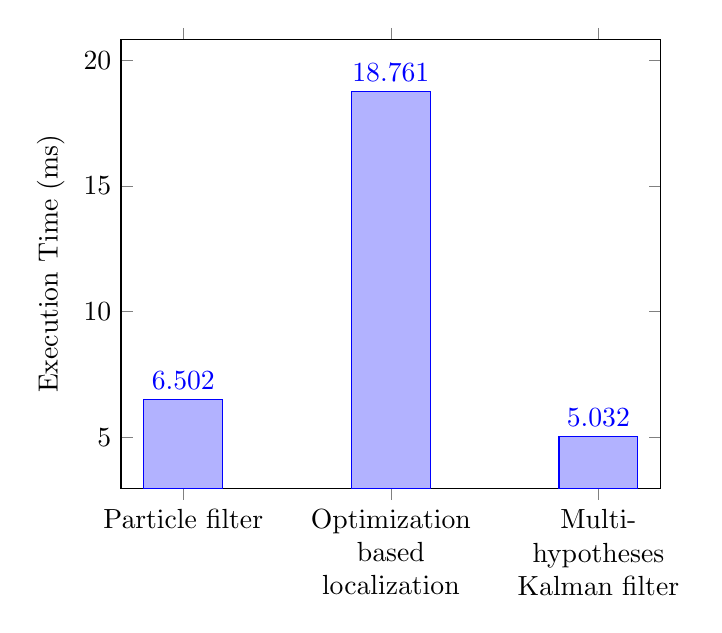
\begin{tikzpicture}
    \begin{axis}[
	ybar,
	enlargelimits=0.15,
	legend style={at={(0.5,-0.15)},
      anchor=north,legend columns=-1},
      ylabel=Execution Time (ms),
      symbolic x coords={Particle filter,Optimization based localization, Multi-hypotheses Kalman filter},
      xtick=data,
      bar width=1cm,
      nodes near coords,
      nodes near coords align={vertical},
      nodes near coords={\pgfmathprintnumber[fixed zerofill, precision=3]{\pgfplotspointmeta}},
    %x tick label style={rotate=-10,anchor=north},
      x tick label style={text width=2.2cm,align=center},
    ]
    %\addplot coordinates {(Particle filter,1.989) (Optimization based,9.952) (Multi-hypotheses Kalman filter, 1.436)};

    %ms per frame on my computer
    %\addplot coordinates {(Particle filter,0.572) (Optimization based localization,2.863) (Multi-hypotheses Kalman filter, 0.413)};

    %ms per frame on NAO
    \addplot coordinates {(Particle filter,6.502) (Optimization based localization,18.761) (Multi-hypotheses Kalman filter, 5.032)};
%\legend{used,understood,not understood}
  \end{axis}
\end{tikzpicture}
\end{table}
%Multi-hypotheses Kalman filter
%Optimization based localization turns out to be 5 times slower than particle filter.



